%        File: arfc-beamer.tex
%     Created: Sun May 5 10:00 PM 2013 C
%


%\documentclass[11pt,handout]{beamer}
\documentclass[9pt]{beamer}
\usetheme[white]{Illinois}
%\title[short title]{long title}
\title[Short Title]{Towards a Holistic Integration of Energy Justice and Energy System Engineering}
%\subtitle[short subtitle]{long subtitle}
\subtitle[Short SubTitle]{Thesis Defense}
%\author[short name]{long name}
\author[Your Name]{Samuel G. Dotson\\Advanced Reactors and Fuel Cycles Group}
%\date[short date]{long date}
\date[10.23.2025]{October 23, 2025}
%\institution[short name]{long name}
\institute[UIUC]{University of Illinois at Urbana-Champaign}

%\usepackage{bbding}
\usepackage{amsfonts}
\usepackage{amsmath}
\usepackage{xspace}
\usepackage{graphicx}
\usepackage{subfigure}
\usepackage{booktabs} % nice rules for tables
\usepackage{microtype} % if using PDF
\usepackage{bigints}
\usepackage{minted}
\usepackage{tikz}
\usepackage{soul}
\usepackage{pgfplots}
\usepackage[table, dvipsnames]{xcolor}



\definecolor{LightGray}{gray}{0.9}
\definecolor{blue1}{HTML}{82C0CC}
\definecolor{blue2}{HTML}{489FB5}
\definecolor{blue3}{HTML}{16697A}
\definecolor{blue4}{HTML}{046354}
\definecolor{blue5}{HTML}{29669E}
\definecolor{blue6}{HTML}{82C0CC}

\definecolor{illiniblue}{HTML}{B1C6E2}
\definecolor{trueilliniblue}{HTML}{13294B}
\definecolor{illiniorange}{HTML}{f8c2a2}
\definecolor{trueilliniorange}{HTML}{E84A27}
\graphicspath{figures/}

\newcommand{\boldblue}[1]{\textcolor{trueilliniblue}{\textbf{#1}}}
\newcommand{\boldorange}[1]{\textcolor{trueilliniorange}{\textbf{#1}}}


% \newtcolorbox{noteBox}[1][]{
%     width=\textwidth,
%     fonttitle=\bfseries,
%     breakable,
%     fonttitle=\bfseries\color{Black},
%     colframe=illiniblue,
%     colback=illiniblue!10
%     #1}

\usetikzlibrary{positioning, arrows, decorations, shapes}
\usetikzlibrary{shapes.geometric,arrows}

\def\checkmark{\tikz\fill[scale=0.4](0,.35) -- (.25,0) -- (1,.7) -- (.25,.15) -- cycle;} 
\tikzstyle{loblock} = [rectangle, draw, fill=illiniorange, 
text width=15em, text centered, rounded corners, minimum height=3em]
\tikzstyle{lbblock} = [rectangle, draw, fill=illiniblue, 
text width=15em, text centered, rounded corners, minimum height=3em]
\tikzstyle{oblock} = [rectangle, draw, fill=illiniorange, 
text width=10em, text centered, rounded corners, minimum height=3em]
\tikzstyle{bblock} = [rectangle, draw, fill=illiniblue, 
text width=10em, text centered, rounded corners, minimum height=3em]
\tikzstyle{arrow} = [thick,->,>=stealth]
\tikzstyle{bbblock} = [rectangle, draw, fill=illiniblue, 
text width=1em, text centered, rounded corners, minimum height=1em]
\tikzstyle{boblock} = [rectangle, draw, fill=illiniorange, 
text width=1em, text centered, rounded corners, minimum height=1em]
\tikzstyle{e72block} = [rectangle, fill=none, 
text width=7.3em, text centered, rounded corners, minimum height=2em]
\tikzstyle{o72block} = [rectangle, draw, fill=illiniorange, 
text width=7.3em, text centered, rounded corners, minimum height=2em]
\tikzstyle{p72block} = [rectangle, draw, fill=purple, 
text width=7.3em, text centered, rounded corners, minimum height=2em]
\tikzstyle{g72block} = [rectangle, draw, fill=green, 
text width=7.3em, text centered, rounded corners, minimum height=2em]
\tikzstyle{b72block} = [rectangle, draw, fill=illiniblue, 
text width=7.3em, text centered, rounded corners, minimum height=2em]
\tikzstyle{e82block} = [rectangle, fill=none, 
text width=8.3em, text centered, rounded corners, minimum height=2em]
\tikzstyle{e92block} = [rectangle, fill=none, 
text width=9.3em, text centered, rounded corners, minimum height=2em]
\tikzstyle{b82block} = [rectangle, draw, fill=illiniblue, 
text width=8em, text centered, rounded corners, minimum height=2em]
\tikzstyle{b223block} = [rectangle, draw, fill=illiniblue, 
text width=22em, text centered, rounded corners, minimum height=3em]

\newcommand{\units}[1] {\:\text{#1}}%
\newcommand{\SN}{S$_N$}%{S$_\text{N}$}%{$S_N$}%
\DeclareMathOperator{\erf}{erf}
%I need some complimentary error funcitons... 
\DeclareMathOperator{\erfc}{erfc}
%Those icons in the references are terrible looking
\setbeamertemplate{bibliography item}[text]
\setbeamertemplate{caption}[numbered]

\newcommand{\mathdefault}[1][]{}

%%%% Acronym support

\usepackage[acronym,toc]{glossaries}
\acro{esom}[ESOM]{energy system optimization model}
\acrodefplural{esom}[ESOMs]{energy system optimization models}
\acro{lp}[LP]{linear programming}
\acrodefplural{lp}[LPs]{linear programs}
\acro{eroi}[EROI]{energy return on investment}
\acro{milp}[MILP]{mixed-integer linear programming}
\acrodefplural{milp}[MILPs]{mixed-integer linear programs}
\acro{osier}[\texttt{Osier}]{Open-source multi-objective energy system framework}
\acro{dapl}[DAPL]{Dakota Access Pipeline}
\acro{temoa}[\texttt{Temoa}]{Tools for Energy Model Optimization and Analysis}
\acro{pygen}[\texttt{PyGenesys}]{Python for Generating Energy Systems}
\acro{pymoo}[\texttt{Pymoo}]{Multi-Objective Optimization in Python}
\acro{pyomo}[\texttt{Pyomo}]{Python-based, open-source optimization modeling language}
\acro{hsj}[HSJ]{Hop-Skip-Jump algorithm}
\acro{mga}[MGA]{Modeling-to-Generate-Alternatives}
\acro{moo}[MOO]{multi-objective optimization}
\acro{ghg}[GHG]{greenhouse gas}
\acrodefplural{ghg}[GHGs]{greenhouse gases}
\acro{sp}[SP]{stochastic programming}
\acro{mc}[MC]{Monte Carlo}
\acro{pa}[PA]{parametric analysis}
\acro{nsga2}[NSGA-II]{Non-Dominated Sorting Genetic Algorithm-II}
\acro{nsga3}[NSGA-III]{Non-Dominated Sorting Genetic Algorithm-III}
\acro{unsga3}[UNSGA-III]{Unified Non-Dominated Sorting Genetic Algorithm}
\acro{ga}[GA]{genetic algorithm}
\acrodefplural{ga}[GAs]{genetic algorithms}
\acro{ws}[WS]{weighted-sum}
\acro{ec}[EC]{$\epsilon$-constraint}
\acro{vre}[VRE]{variable renewable energy}
\acro{nrc}[NRC]{Nuclear Regulatory Commission}
\acro{nrel}[NREL]{National Renewable Energy Laboratory}
\acro{atb}[ATB]{Annual Technology Baseline}
\acro{stm}[STM]{social transition movement}
\acro{ccs}[CCS]{carbon capture and storage}
\acro{pve}[PVE]{participatory value evaluation}
\acro{ipcc}[IPCC]{International Panel on Climate Change}
\acro{un}[UN]{United Nations}
\acro{gva}[GVA]{gross value added}
\acro{gdp}[GDP]{gross domestic product}
\acro{wtp}[WTP]{willingness to pay}
\acro{wpe}[WPE]{weighted permutation entropy}
\acro{igdp}[IGD+]{inverted generational distance plus}
\acro{icap}[iCAP]{Illinois Climate Action Plan}
\acro{isee}[iSEE]{Institute for Sustainability, Energy, and Environment}
\acro{ipcc}[IPCC]{International Panel on Climate Change}
\acro{deap}[\texttt{DEAP}]{Deep Evolutionary Algorithms in Python}
\acro{uiuc}[UIUC]{University of Illinois Urbana-Champaign}
\acro{pcp}[PCP]{parallel coordinate plot}
\acro{nimby}[NIMBY]{not-in-my-backyard}
\acro{nimbyism}[NIMBYism]{not-in-my-backyard}
\acro{snf}[SNF]{spent-nuclear-fuel}
\acro{smr}[SMR]{small modular reactor}
\acrodefplural{smr}[SMRs]{small modular reactors}
\acro{ipa}[IPA]{Illinois Power Agency}
\acro{icc}[ICC]{Illinois Commerce Commission}
\acro{set}[SET tool]{Screening and Evaluation Tool}
\acro{mca}[MCA]{municipal choice aggregation}
\acro{imea}[IMEA]{Illinois Municipal Electric Agency}
\acro{ppa}[PPA]{power purchase agreement}
\acro{pypsa}[\texttt{PyPSA}]{Python for Power Systems Analysis}
\acro{lib}[LiB]{lithium-ion battery}
\acrodefplural{lib}[LiBs]{lithium-ion batteries}
\acro{reason}[RE$^3$ASON]{Renewable Energies and Energy Efficiency Analysis and System Optimization}
\acro{mavt}[MAVT]{multi-attribute value theory}
\acro{mcda}[MCDA]{multi-criteria decision analysis}
\acro{ngo}[NGO]{non-governmental organization}
\acro{co2}[CO$_2$]{carbon dioxide}
\acro{co2eq}[CO$_2$-eq]{CO$_2$-equivalent}
% \usepackage{acronym}
% \newcommand{\acro}[3]{\acrodef{#1}[#2]{#3}}


% \makeglossaries

%try to get rid of header on title page\dots
\makeatletter
    \newenvironment{withoutheadline}{
        \setbeamertemplate{headline}[default]
        \def\beamer@entrycode{\vspace*{-\headheight}}
    }{}
\makeatother

\makeatother
\setbeamertemplate{footline}
{
  \leavevmode%
  \hbox{%
    \rightline{\insertframenumber{} / \inserttotalframenumber\hspace*{1ex}}
  }%
  \vskip0pt%
}
\makeatletter
\begin{document}
%%%%%%%%%%%%%%%%%%%%%%%%%%%%%%%%%%%%%%%%%%%%%%%%%%%%%%%%%%%%%
%% From uw-beamer Here's a handy bit of code to place at 
%% the beginning of your presentation (after \begin{document}):
\newcommand*{\alphabet}{ABCDEFGHIJKLMNOPQRSTUVWXYZabcdefghijklmnopqrstuvwxyz}
\newlength{\highlightheight}
\newlength{\highlightdepth}
\newlength{\highlightmargin}
\setlength{\highlightmargin}{2pt}
\settoheight{\highlightheight}{\alphabet}
\settodepth{\highlightdepth}{\alphabet}
\addtolength{\highlightheight}{\highlightmargin}
\addtolength{\highlightdepth}{\highlightmargin}
\addtolength{\highlightheight}{\highlightdepth}
\newcommand*{\Highlight}{\rlap{\textcolor{HighlightBackground}{\rule[-\highlightdepth]{\linewidth}{\highlightheight}}}}
%%%%%%%%%%%%%%%%%%%%%%%%%%%%%%%%%%%%%%%%%%%%%%%%%%%%%%%%%%%%%
%%--------------------------------%%
\begin{withoutheadline}
\frame{
  \titlepage
}
\end{withoutheadline}

%%--------------------------------%%
\AtBeginSection[]{
\begin{frame}[allowframebreaks]
  \frametitle{Outline}
  \tableofcontents[currentsection]
\end{frame}
}

\section{Introduction}

\subsection{Background}

\begin{frame}
    \frametitle{The Clean Energy Transition}
    Our changing climate and additional demand drivers from data 
    centers and \gls{ai} require a just transition from fossil 
    fuels to clean energy.
    \begin{columns}
        \column[t]{5.5cm}    
        \begin{figure}
            \centering
            \resizebox{\columnwidth}{!}{%% Creator: Matplotlib, PGF backend
%%
%% To include the figure in your LaTeX document, write
%%   \input{<filename>.pgf}
%%
%% Make sure the required packages are loaded in your preamble
%%   \usepackage{pgf}
%%
%% Also ensure that all the required font packages are loaded; for instance,
%% the lmodern package is sometimes necessary when using math font.
%%   \usepackage{lmodern}
%%
%% Figures using additional raster images can only be included by \input if
%% they are in the same directory as the main LaTeX file. For loading figures
%% from other directories you can use the `import` package
%%   \usepackage{import}
%%
%% and then include the figures with
%%   \import{<path to file>}{<filename>.pgf}
%%
%% Matplotlib used the following preamble
%%   \def\mathdefault#1{#1}
%%   \everymath=\expandafter{\the\everymath\displaystyle}
%%   \IfFileExists{scrextend.sty}{
%%     \usepackage[fontsize=10.000000pt]{scrextend}
%%   }{
%%     \renewcommand{\normalsize}{\fontsize{10.000000}{12.000000}\selectfont}
%%     \normalsize
%%   }
%%   
%%   \makeatletter\@ifpackageloaded{underscore}{}{\usepackage[strings]{underscore}}\makeatother
%%
\begingroup%
\makeatletter%
\begin{pgfpicture}%
\pgfpathrectangle{\pgfpointorigin}{\pgfqpoint{7.880511in}{5.900000in}}%
\pgfusepath{use as bounding box, clip}%
\begin{pgfscope}%
\pgfsetbuttcap%
\pgfsetmiterjoin%
\definecolor{currentfill}{rgb}{1.000000,1.000000,1.000000}%
\pgfsetfillcolor{currentfill}%
\pgfsetlinewidth{0.000000pt}%
\definecolor{currentstroke}{rgb}{0.000000,0.000000,0.000000}%
\pgfsetstrokecolor{currentstroke}%
\pgfsetdash{}{0pt}%
\pgfpathmoveto{\pgfqpoint{0.000000in}{0.000000in}}%
\pgfpathlineto{\pgfqpoint{7.880511in}{0.000000in}}%
\pgfpathlineto{\pgfqpoint{7.880511in}{5.900000in}}%
\pgfpathlineto{\pgfqpoint{0.000000in}{5.900000in}}%
\pgfpathlineto{\pgfqpoint{0.000000in}{0.000000in}}%
\pgfpathclose%
\pgfusepath{fill}%
\end{pgfscope}%
\begin{pgfscope}%
\pgfsetbuttcap%
\pgfsetmiterjoin%
\definecolor{currentfill}{rgb}{1.000000,1.000000,1.000000}%
\pgfsetfillcolor{currentfill}%
\pgfsetlinewidth{0.000000pt}%
\definecolor{currentstroke}{rgb}{0.000000,0.000000,0.000000}%
\pgfsetstrokecolor{currentstroke}%
\pgfsetstrokeopacity{0.000000}%
\pgfsetdash{}{0pt}%
\pgfpathmoveto{\pgfqpoint{0.697913in}{0.559721in}}%
\pgfpathlineto{\pgfqpoint{7.746549in}{0.559721in}}%
\pgfpathlineto{\pgfqpoint{7.746549in}{5.550000in}}%
\pgfpathlineto{\pgfqpoint{0.697913in}{5.550000in}}%
\pgfpathlineto{\pgfqpoint{0.697913in}{0.559721in}}%
\pgfpathclose%
\pgfusepath{fill}%
\end{pgfscope}%
\begin{pgfscope}%
\pgfpathrectangle{\pgfqpoint{0.697913in}{0.559721in}}{\pgfqpoint{7.048636in}{4.990279in}}%
\pgfusepath{clip}%
\pgfsetrectcap%
\pgfsetroundjoin%
\pgfsetlinewidth{0.803000pt}%
\definecolor{currentstroke}{rgb}{0.690196,0.690196,0.690196}%
\pgfsetstrokecolor{currentstroke}%
\pgfsetdash{}{0pt}%
\pgfpathmoveto{\pgfqpoint{1.404248in}{0.559721in}}%
\pgfpathlineto{\pgfqpoint{1.404248in}{5.550000in}}%
\pgfusepath{stroke}%
\end{pgfscope}%
\begin{pgfscope}%
\pgfsetbuttcap%
\pgfsetroundjoin%
\definecolor{currentfill}{rgb}{0.000000,0.000000,0.000000}%
\pgfsetfillcolor{currentfill}%
\pgfsetlinewidth{1.254687pt}%
\definecolor{currentstroke}{rgb}{0.000000,0.000000,0.000000}%
\pgfsetstrokecolor{currentstroke}%
\pgfsetdash{}{0pt}%
\pgfsys@defobject{currentmarker}{\pgfqpoint{0.000000in}{0.000000in}}{\pgfqpoint{0.000000in}{0.111111in}}{%
\pgfpathmoveto{\pgfqpoint{0.000000in}{0.000000in}}%
\pgfpathlineto{\pgfqpoint{0.000000in}{0.111111in}}%
\pgfusepath{stroke,fill}%
}%
\begin{pgfscope}%
\pgfsys@transformshift{1.404248in}{0.559721in}%
\pgfsys@useobject{currentmarker}{}%
\end{pgfscope}%
\end{pgfscope}%
\begin{pgfscope}%
\definecolor{textcolor}{rgb}{0.000000,0.000000,0.000000}%
\pgfsetstrokecolor{textcolor}%
\pgfsetfillcolor{textcolor}%
\pgftext[x=1.404248in,y=0.511110in,,top]{\color{textcolor}{\rmfamily\fontsize{14.000000}{16.800000}\selectfont\catcode`\^=\active\def^{\ifmmode\sp\else\^{}\fi}\catcode`\%=\active\def%{\%}1989}}%
\end{pgfscope}%
\begin{pgfscope}%
\pgfpathrectangle{\pgfqpoint{0.697913in}{0.559721in}}{\pgfqpoint{7.048636in}{4.990279in}}%
\pgfusepath{clip}%
\pgfsetrectcap%
\pgfsetroundjoin%
\pgfsetlinewidth{0.803000pt}%
\definecolor{currentstroke}{rgb}{0.690196,0.690196,0.690196}%
\pgfsetstrokecolor{currentstroke}%
\pgfsetdash{}{0pt}%
\pgfpathmoveto{\pgfqpoint{2.287167in}{0.559721in}}%
\pgfpathlineto{\pgfqpoint{2.287167in}{5.550000in}}%
\pgfusepath{stroke}%
\end{pgfscope}%
\begin{pgfscope}%
\pgfsetbuttcap%
\pgfsetroundjoin%
\definecolor{currentfill}{rgb}{0.000000,0.000000,0.000000}%
\pgfsetfillcolor{currentfill}%
\pgfsetlinewidth{1.254687pt}%
\definecolor{currentstroke}{rgb}{0.000000,0.000000,0.000000}%
\pgfsetstrokecolor{currentstroke}%
\pgfsetdash{}{0pt}%
\pgfsys@defobject{currentmarker}{\pgfqpoint{0.000000in}{0.000000in}}{\pgfqpoint{0.000000in}{0.111111in}}{%
\pgfpathmoveto{\pgfqpoint{0.000000in}{0.000000in}}%
\pgfpathlineto{\pgfqpoint{0.000000in}{0.111111in}}%
\pgfusepath{stroke,fill}%
}%
\begin{pgfscope}%
\pgfsys@transformshift{2.287167in}{0.559721in}%
\pgfsys@useobject{currentmarker}{}%
\end{pgfscope}%
\end{pgfscope}%
\begin{pgfscope}%
\definecolor{textcolor}{rgb}{0.000000,0.000000,0.000000}%
\pgfsetstrokecolor{textcolor}%
\pgfsetfillcolor{textcolor}%
\pgftext[x=2.287167in,y=0.511110in,,top]{\color{textcolor}{\rmfamily\fontsize{14.000000}{16.800000}\selectfont\catcode`\^=\active\def^{\ifmmode\sp\else\^{}\fi}\catcode`\%=\active\def%{\%}1994}}%
\end{pgfscope}%
\begin{pgfscope}%
\pgfpathrectangle{\pgfqpoint{0.697913in}{0.559721in}}{\pgfqpoint{7.048636in}{4.990279in}}%
\pgfusepath{clip}%
\pgfsetrectcap%
\pgfsetroundjoin%
\pgfsetlinewidth{0.803000pt}%
\definecolor{currentstroke}{rgb}{0.690196,0.690196,0.690196}%
\pgfsetstrokecolor{currentstroke}%
\pgfsetdash{}{0pt}%
\pgfpathmoveto{\pgfqpoint{3.170086in}{0.559721in}}%
\pgfpathlineto{\pgfqpoint{3.170086in}{5.550000in}}%
\pgfusepath{stroke}%
\end{pgfscope}%
\begin{pgfscope}%
\pgfsetbuttcap%
\pgfsetroundjoin%
\definecolor{currentfill}{rgb}{0.000000,0.000000,0.000000}%
\pgfsetfillcolor{currentfill}%
\pgfsetlinewidth{1.254687pt}%
\definecolor{currentstroke}{rgb}{0.000000,0.000000,0.000000}%
\pgfsetstrokecolor{currentstroke}%
\pgfsetdash{}{0pt}%
\pgfsys@defobject{currentmarker}{\pgfqpoint{0.000000in}{0.000000in}}{\pgfqpoint{0.000000in}{0.111111in}}{%
\pgfpathmoveto{\pgfqpoint{0.000000in}{0.000000in}}%
\pgfpathlineto{\pgfqpoint{0.000000in}{0.111111in}}%
\pgfusepath{stroke,fill}%
}%
\begin{pgfscope}%
\pgfsys@transformshift{3.170086in}{0.559721in}%
\pgfsys@useobject{currentmarker}{}%
\end{pgfscope}%
\end{pgfscope}%
\begin{pgfscope}%
\definecolor{textcolor}{rgb}{0.000000,0.000000,0.000000}%
\pgfsetstrokecolor{textcolor}%
\pgfsetfillcolor{textcolor}%
\pgftext[x=3.170086in,y=0.511110in,,top]{\color{textcolor}{\rmfamily\fontsize{14.000000}{16.800000}\selectfont\catcode`\^=\active\def^{\ifmmode\sp\else\^{}\fi}\catcode`\%=\active\def%{\%}1999}}%
\end{pgfscope}%
\begin{pgfscope}%
\pgfpathrectangle{\pgfqpoint{0.697913in}{0.559721in}}{\pgfqpoint{7.048636in}{4.990279in}}%
\pgfusepath{clip}%
\pgfsetrectcap%
\pgfsetroundjoin%
\pgfsetlinewidth{0.803000pt}%
\definecolor{currentstroke}{rgb}{0.690196,0.690196,0.690196}%
\pgfsetstrokecolor{currentstroke}%
\pgfsetdash{}{0pt}%
\pgfpathmoveto{\pgfqpoint{4.053005in}{0.559721in}}%
\pgfpathlineto{\pgfqpoint{4.053005in}{5.550000in}}%
\pgfusepath{stroke}%
\end{pgfscope}%
\begin{pgfscope}%
\pgfsetbuttcap%
\pgfsetroundjoin%
\definecolor{currentfill}{rgb}{0.000000,0.000000,0.000000}%
\pgfsetfillcolor{currentfill}%
\pgfsetlinewidth{1.254687pt}%
\definecolor{currentstroke}{rgb}{0.000000,0.000000,0.000000}%
\pgfsetstrokecolor{currentstroke}%
\pgfsetdash{}{0pt}%
\pgfsys@defobject{currentmarker}{\pgfqpoint{0.000000in}{0.000000in}}{\pgfqpoint{0.000000in}{0.111111in}}{%
\pgfpathmoveto{\pgfqpoint{0.000000in}{0.000000in}}%
\pgfpathlineto{\pgfqpoint{0.000000in}{0.111111in}}%
\pgfusepath{stroke,fill}%
}%
\begin{pgfscope}%
\pgfsys@transformshift{4.053005in}{0.559721in}%
\pgfsys@useobject{currentmarker}{}%
\end{pgfscope}%
\end{pgfscope}%
\begin{pgfscope}%
\definecolor{textcolor}{rgb}{0.000000,0.000000,0.000000}%
\pgfsetstrokecolor{textcolor}%
\pgfsetfillcolor{textcolor}%
\pgftext[x=4.053005in,y=0.511110in,,top]{\color{textcolor}{\rmfamily\fontsize{14.000000}{16.800000}\selectfont\catcode`\^=\active\def^{\ifmmode\sp\else\^{}\fi}\catcode`\%=\active\def%{\%}2004}}%
\end{pgfscope}%
\begin{pgfscope}%
\pgfpathrectangle{\pgfqpoint{0.697913in}{0.559721in}}{\pgfqpoint{7.048636in}{4.990279in}}%
\pgfusepath{clip}%
\pgfsetrectcap%
\pgfsetroundjoin%
\pgfsetlinewidth{0.803000pt}%
\definecolor{currentstroke}{rgb}{0.690196,0.690196,0.690196}%
\pgfsetstrokecolor{currentstroke}%
\pgfsetdash{}{0pt}%
\pgfpathmoveto{\pgfqpoint{4.935924in}{0.559721in}}%
\pgfpathlineto{\pgfqpoint{4.935924in}{5.550000in}}%
\pgfusepath{stroke}%
\end{pgfscope}%
\begin{pgfscope}%
\pgfsetbuttcap%
\pgfsetroundjoin%
\definecolor{currentfill}{rgb}{0.000000,0.000000,0.000000}%
\pgfsetfillcolor{currentfill}%
\pgfsetlinewidth{1.254687pt}%
\definecolor{currentstroke}{rgb}{0.000000,0.000000,0.000000}%
\pgfsetstrokecolor{currentstroke}%
\pgfsetdash{}{0pt}%
\pgfsys@defobject{currentmarker}{\pgfqpoint{0.000000in}{0.000000in}}{\pgfqpoint{0.000000in}{0.111111in}}{%
\pgfpathmoveto{\pgfqpoint{0.000000in}{0.000000in}}%
\pgfpathlineto{\pgfqpoint{0.000000in}{0.111111in}}%
\pgfusepath{stroke,fill}%
}%
\begin{pgfscope}%
\pgfsys@transformshift{4.935924in}{0.559721in}%
\pgfsys@useobject{currentmarker}{}%
\end{pgfscope}%
\end{pgfscope}%
\begin{pgfscope}%
\definecolor{textcolor}{rgb}{0.000000,0.000000,0.000000}%
\pgfsetstrokecolor{textcolor}%
\pgfsetfillcolor{textcolor}%
\pgftext[x=4.935924in,y=0.511110in,,top]{\color{textcolor}{\rmfamily\fontsize{14.000000}{16.800000}\selectfont\catcode`\^=\active\def^{\ifmmode\sp\else\^{}\fi}\catcode`\%=\active\def%{\%}2009}}%
\end{pgfscope}%
\begin{pgfscope}%
\pgfpathrectangle{\pgfqpoint{0.697913in}{0.559721in}}{\pgfqpoint{7.048636in}{4.990279in}}%
\pgfusepath{clip}%
\pgfsetrectcap%
\pgfsetroundjoin%
\pgfsetlinewidth{0.803000pt}%
\definecolor{currentstroke}{rgb}{0.690196,0.690196,0.690196}%
\pgfsetstrokecolor{currentstroke}%
\pgfsetdash{}{0pt}%
\pgfpathmoveto{\pgfqpoint{5.818843in}{0.559721in}}%
\pgfpathlineto{\pgfqpoint{5.818843in}{5.550000in}}%
\pgfusepath{stroke}%
\end{pgfscope}%
\begin{pgfscope}%
\pgfsetbuttcap%
\pgfsetroundjoin%
\definecolor{currentfill}{rgb}{0.000000,0.000000,0.000000}%
\pgfsetfillcolor{currentfill}%
\pgfsetlinewidth{1.254687pt}%
\definecolor{currentstroke}{rgb}{0.000000,0.000000,0.000000}%
\pgfsetstrokecolor{currentstroke}%
\pgfsetdash{}{0pt}%
\pgfsys@defobject{currentmarker}{\pgfqpoint{0.000000in}{0.000000in}}{\pgfqpoint{0.000000in}{0.111111in}}{%
\pgfpathmoveto{\pgfqpoint{0.000000in}{0.000000in}}%
\pgfpathlineto{\pgfqpoint{0.000000in}{0.111111in}}%
\pgfusepath{stroke,fill}%
}%
\begin{pgfscope}%
\pgfsys@transformshift{5.818843in}{0.559721in}%
\pgfsys@useobject{currentmarker}{}%
\end{pgfscope}%
\end{pgfscope}%
\begin{pgfscope}%
\definecolor{textcolor}{rgb}{0.000000,0.000000,0.000000}%
\pgfsetstrokecolor{textcolor}%
\pgfsetfillcolor{textcolor}%
\pgftext[x=5.818843in,y=0.511110in,,top]{\color{textcolor}{\rmfamily\fontsize{14.000000}{16.800000}\selectfont\catcode`\^=\active\def^{\ifmmode\sp\else\^{}\fi}\catcode`\%=\active\def%{\%}2014}}%
\end{pgfscope}%
\begin{pgfscope}%
\pgfpathrectangle{\pgfqpoint{0.697913in}{0.559721in}}{\pgfqpoint{7.048636in}{4.990279in}}%
\pgfusepath{clip}%
\pgfsetrectcap%
\pgfsetroundjoin%
\pgfsetlinewidth{0.803000pt}%
\definecolor{currentstroke}{rgb}{0.690196,0.690196,0.690196}%
\pgfsetstrokecolor{currentstroke}%
\pgfsetdash{}{0pt}%
\pgfpathmoveto{\pgfqpoint{6.701762in}{0.559721in}}%
\pgfpathlineto{\pgfqpoint{6.701762in}{5.550000in}}%
\pgfusepath{stroke}%
\end{pgfscope}%
\begin{pgfscope}%
\pgfsetbuttcap%
\pgfsetroundjoin%
\definecolor{currentfill}{rgb}{0.000000,0.000000,0.000000}%
\pgfsetfillcolor{currentfill}%
\pgfsetlinewidth{1.254687pt}%
\definecolor{currentstroke}{rgb}{0.000000,0.000000,0.000000}%
\pgfsetstrokecolor{currentstroke}%
\pgfsetdash{}{0pt}%
\pgfsys@defobject{currentmarker}{\pgfqpoint{0.000000in}{0.000000in}}{\pgfqpoint{0.000000in}{0.111111in}}{%
\pgfpathmoveto{\pgfqpoint{0.000000in}{0.000000in}}%
\pgfpathlineto{\pgfqpoint{0.000000in}{0.111111in}}%
\pgfusepath{stroke,fill}%
}%
\begin{pgfscope}%
\pgfsys@transformshift{6.701762in}{0.559721in}%
\pgfsys@useobject{currentmarker}{}%
\end{pgfscope}%
\end{pgfscope}%
\begin{pgfscope}%
\definecolor{textcolor}{rgb}{0.000000,0.000000,0.000000}%
\pgfsetstrokecolor{textcolor}%
\pgfsetfillcolor{textcolor}%
\pgftext[x=6.701762in,y=0.511110in,,top]{\color{textcolor}{\rmfamily\fontsize{14.000000}{16.800000}\selectfont\catcode`\^=\active\def^{\ifmmode\sp\else\^{}\fi}\catcode`\%=\active\def%{\%}2019}}%
\end{pgfscope}%
\begin{pgfscope}%
\pgfpathrectangle{\pgfqpoint{0.697913in}{0.559721in}}{\pgfqpoint{7.048636in}{4.990279in}}%
\pgfusepath{clip}%
\pgfsetrectcap%
\pgfsetroundjoin%
\pgfsetlinewidth{0.803000pt}%
\definecolor{currentstroke}{rgb}{0.690196,0.690196,0.690196}%
\pgfsetstrokecolor{currentstroke}%
\pgfsetdash{}{0pt}%
\pgfpathmoveto{\pgfqpoint{7.584681in}{0.559721in}}%
\pgfpathlineto{\pgfqpoint{7.584681in}{5.550000in}}%
\pgfusepath{stroke}%
\end{pgfscope}%
\begin{pgfscope}%
\pgfsetbuttcap%
\pgfsetroundjoin%
\definecolor{currentfill}{rgb}{0.000000,0.000000,0.000000}%
\pgfsetfillcolor{currentfill}%
\pgfsetlinewidth{1.254687pt}%
\definecolor{currentstroke}{rgb}{0.000000,0.000000,0.000000}%
\pgfsetstrokecolor{currentstroke}%
\pgfsetdash{}{0pt}%
\pgfsys@defobject{currentmarker}{\pgfqpoint{0.000000in}{0.000000in}}{\pgfqpoint{0.000000in}{0.111111in}}{%
\pgfpathmoveto{\pgfqpoint{0.000000in}{0.000000in}}%
\pgfpathlineto{\pgfqpoint{0.000000in}{0.111111in}}%
\pgfusepath{stroke,fill}%
}%
\begin{pgfscope}%
\pgfsys@transformshift{7.584681in}{0.559721in}%
\pgfsys@useobject{currentmarker}{}%
\end{pgfscope}%
\end{pgfscope}%
\begin{pgfscope}%
\definecolor{textcolor}{rgb}{0.000000,0.000000,0.000000}%
\pgfsetstrokecolor{textcolor}%
\pgfsetfillcolor{textcolor}%
\pgftext[x=7.584681in,y=0.511110in,,top]{\color{textcolor}{\rmfamily\fontsize{14.000000}{16.800000}\selectfont\catcode`\^=\active\def^{\ifmmode\sp\else\^{}\fi}\catcode`\%=\active\def%{\%}2024}}%
\end{pgfscope}%
\begin{pgfscope}%
\pgfsetbuttcap%
\pgfsetroundjoin%
\definecolor{currentfill}{rgb}{0.000000,0.000000,0.000000}%
\pgfsetfillcolor{currentfill}%
\pgfsetlinewidth{1.254687pt}%
\definecolor{currentstroke}{rgb}{0.000000,0.000000,0.000000}%
\pgfsetstrokecolor{currentstroke}%
\pgfsetdash{}{0pt}%
\pgfsys@defobject{currentmarker}{\pgfqpoint{0.000000in}{0.000000in}}{\pgfqpoint{0.000000in}{0.055556in}}{%
\pgfpathmoveto{\pgfqpoint{0.000000in}{0.000000in}}%
\pgfpathlineto{\pgfqpoint{0.000000in}{0.055556in}}%
\pgfusepath{stroke,fill}%
}%
\begin{pgfscope}%
\pgfsys@transformshift{0.742059in}{0.559721in}%
\pgfsys@useobject{currentmarker}{}%
\end{pgfscope}%
\end{pgfscope}%
\begin{pgfscope}%
\pgfsetbuttcap%
\pgfsetroundjoin%
\definecolor{currentfill}{rgb}{0.000000,0.000000,0.000000}%
\pgfsetfillcolor{currentfill}%
\pgfsetlinewidth{1.254687pt}%
\definecolor{currentstroke}{rgb}{0.000000,0.000000,0.000000}%
\pgfsetstrokecolor{currentstroke}%
\pgfsetdash{}{0pt}%
\pgfsys@defobject{currentmarker}{\pgfqpoint{0.000000in}{0.000000in}}{\pgfqpoint{0.000000in}{0.055556in}}{%
\pgfpathmoveto{\pgfqpoint{0.000000in}{0.000000in}}%
\pgfpathlineto{\pgfqpoint{0.000000in}{0.055556in}}%
\pgfusepath{stroke,fill}%
}%
\begin{pgfscope}%
\pgfsys@transformshift{0.962788in}{0.559721in}%
\pgfsys@useobject{currentmarker}{}%
\end{pgfscope}%
\end{pgfscope}%
\begin{pgfscope}%
\pgfsetbuttcap%
\pgfsetroundjoin%
\definecolor{currentfill}{rgb}{0.000000,0.000000,0.000000}%
\pgfsetfillcolor{currentfill}%
\pgfsetlinewidth{1.254687pt}%
\definecolor{currentstroke}{rgb}{0.000000,0.000000,0.000000}%
\pgfsetstrokecolor{currentstroke}%
\pgfsetdash{}{0pt}%
\pgfsys@defobject{currentmarker}{\pgfqpoint{0.000000in}{0.000000in}}{\pgfqpoint{0.000000in}{0.055556in}}{%
\pgfpathmoveto{\pgfqpoint{0.000000in}{0.000000in}}%
\pgfpathlineto{\pgfqpoint{0.000000in}{0.055556in}}%
\pgfusepath{stroke,fill}%
}%
\begin{pgfscope}%
\pgfsys@transformshift{1.183518in}{0.559721in}%
\pgfsys@useobject{currentmarker}{}%
\end{pgfscope}%
\end{pgfscope}%
\begin{pgfscope}%
\pgfsetbuttcap%
\pgfsetroundjoin%
\definecolor{currentfill}{rgb}{0.000000,0.000000,0.000000}%
\pgfsetfillcolor{currentfill}%
\pgfsetlinewidth{1.254687pt}%
\definecolor{currentstroke}{rgb}{0.000000,0.000000,0.000000}%
\pgfsetstrokecolor{currentstroke}%
\pgfsetdash{}{0pt}%
\pgfsys@defobject{currentmarker}{\pgfqpoint{0.000000in}{0.000000in}}{\pgfqpoint{0.000000in}{0.055556in}}{%
\pgfpathmoveto{\pgfqpoint{0.000000in}{0.000000in}}%
\pgfpathlineto{\pgfqpoint{0.000000in}{0.055556in}}%
\pgfusepath{stroke,fill}%
}%
\begin{pgfscope}%
\pgfsys@transformshift{1.624978in}{0.559721in}%
\pgfsys@useobject{currentmarker}{}%
\end{pgfscope}%
\end{pgfscope}%
\begin{pgfscope}%
\pgfsetbuttcap%
\pgfsetroundjoin%
\definecolor{currentfill}{rgb}{0.000000,0.000000,0.000000}%
\pgfsetfillcolor{currentfill}%
\pgfsetlinewidth{1.254687pt}%
\definecolor{currentstroke}{rgb}{0.000000,0.000000,0.000000}%
\pgfsetstrokecolor{currentstroke}%
\pgfsetdash{}{0pt}%
\pgfsys@defobject{currentmarker}{\pgfqpoint{0.000000in}{0.000000in}}{\pgfqpoint{0.000000in}{0.055556in}}{%
\pgfpathmoveto{\pgfqpoint{0.000000in}{0.000000in}}%
\pgfpathlineto{\pgfqpoint{0.000000in}{0.055556in}}%
\pgfusepath{stroke,fill}%
}%
\begin{pgfscope}%
\pgfsys@transformshift{1.845707in}{0.559721in}%
\pgfsys@useobject{currentmarker}{}%
\end{pgfscope}%
\end{pgfscope}%
\begin{pgfscope}%
\pgfsetbuttcap%
\pgfsetroundjoin%
\definecolor{currentfill}{rgb}{0.000000,0.000000,0.000000}%
\pgfsetfillcolor{currentfill}%
\pgfsetlinewidth{1.254687pt}%
\definecolor{currentstroke}{rgb}{0.000000,0.000000,0.000000}%
\pgfsetstrokecolor{currentstroke}%
\pgfsetdash{}{0pt}%
\pgfsys@defobject{currentmarker}{\pgfqpoint{0.000000in}{0.000000in}}{\pgfqpoint{0.000000in}{0.055556in}}{%
\pgfpathmoveto{\pgfqpoint{0.000000in}{0.000000in}}%
\pgfpathlineto{\pgfqpoint{0.000000in}{0.055556in}}%
\pgfusepath{stroke,fill}%
}%
\begin{pgfscope}%
\pgfsys@transformshift{2.066437in}{0.559721in}%
\pgfsys@useobject{currentmarker}{}%
\end{pgfscope}%
\end{pgfscope}%
\begin{pgfscope}%
\pgfsetbuttcap%
\pgfsetroundjoin%
\definecolor{currentfill}{rgb}{0.000000,0.000000,0.000000}%
\pgfsetfillcolor{currentfill}%
\pgfsetlinewidth{1.254687pt}%
\definecolor{currentstroke}{rgb}{0.000000,0.000000,0.000000}%
\pgfsetstrokecolor{currentstroke}%
\pgfsetdash{}{0pt}%
\pgfsys@defobject{currentmarker}{\pgfqpoint{0.000000in}{0.000000in}}{\pgfqpoint{0.000000in}{0.055556in}}{%
\pgfpathmoveto{\pgfqpoint{0.000000in}{0.000000in}}%
\pgfpathlineto{\pgfqpoint{0.000000in}{0.055556in}}%
\pgfusepath{stroke,fill}%
}%
\begin{pgfscope}%
\pgfsys@transformshift{2.507897in}{0.559721in}%
\pgfsys@useobject{currentmarker}{}%
\end{pgfscope}%
\end{pgfscope}%
\begin{pgfscope}%
\pgfsetbuttcap%
\pgfsetroundjoin%
\definecolor{currentfill}{rgb}{0.000000,0.000000,0.000000}%
\pgfsetfillcolor{currentfill}%
\pgfsetlinewidth{1.254687pt}%
\definecolor{currentstroke}{rgb}{0.000000,0.000000,0.000000}%
\pgfsetstrokecolor{currentstroke}%
\pgfsetdash{}{0pt}%
\pgfsys@defobject{currentmarker}{\pgfqpoint{0.000000in}{0.000000in}}{\pgfqpoint{0.000000in}{0.055556in}}{%
\pgfpathmoveto{\pgfqpoint{0.000000in}{0.000000in}}%
\pgfpathlineto{\pgfqpoint{0.000000in}{0.055556in}}%
\pgfusepath{stroke,fill}%
}%
\begin{pgfscope}%
\pgfsys@transformshift{2.728626in}{0.559721in}%
\pgfsys@useobject{currentmarker}{}%
\end{pgfscope}%
\end{pgfscope}%
\begin{pgfscope}%
\pgfsetbuttcap%
\pgfsetroundjoin%
\definecolor{currentfill}{rgb}{0.000000,0.000000,0.000000}%
\pgfsetfillcolor{currentfill}%
\pgfsetlinewidth{1.254687pt}%
\definecolor{currentstroke}{rgb}{0.000000,0.000000,0.000000}%
\pgfsetstrokecolor{currentstroke}%
\pgfsetdash{}{0pt}%
\pgfsys@defobject{currentmarker}{\pgfqpoint{0.000000in}{0.000000in}}{\pgfqpoint{0.000000in}{0.055556in}}{%
\pgfpathmoveto{\pgfqpoint{0.000000in}{0.000000in}}%
\pgfpathlineto{\pgfqpoint{0.000000in}{0.055556in}}%
\pgfusepath{stroke,fill}%
}%
\begin{pgfscope}%
\pgfsys@transformshift{2.949356in}{0.559721in}%
\pgfsys@useobject{currentmarker}{}%
\end{pgfscope}%
\end{pgfscope}%
\begin{pgfscope}%
\pgfsetbuttcap%
\pgfsetroundjoin%
\definecolor{currentfill}{rgb}{0.000000,0.000000,0.000000}%
\pgfsetfillcolor{currentfill}%
\pgfsetlinewidth{1.254687pt}%
\definecolor{currentstroke}{rgb}{0.000000,0.000000,0.000000}%
\pgfsetstrokecolor{currentstroke}%
\pgfsetdash{}{0pt}%
\pgfsys@defobject{currentmarker}{\pgfqpoint{0.000000in}{0.000000in}}{\pgfqpoint{0.000000in}{0.055556in}}{%
\pgfpathmoveto{\pgfqpoint{0.000000in}{0.000000in}}%
\pgfpathlineto{\pgfqpoint{0.000000in}{0.055556in}}%
\pgfusepath{stroke,fill}%
}%
\begin{pgfscope}%
\pgfsys@transformshift{3.390815in}{0.559721in}%
\pgfsys@useobject{currentmarker}{}%
\end{pgfscope}%
\end{pgfscope}%
\begin{pgfscope}%
\pgfsetbuttcap%
\pgfsetroundjoin%
\definecolor{currentfill}{rgb}{0.000000,0.000000,0.000000}%
\pgfsetfillcolor{currentfill}%
\pgfsetlinewidth{1.254687pt}%
\definecolor{currentstroke}{rgb}{0.000000,0.000000,0.000000}%
\pgfsetstrokecolor{currentstroke}%
\pgfsetdash{}{0pt}%
\pgfsys@defobject{currentmarker}{\pgfqpoint{0.000000in}{0.000000in}}{\pgfqpoint{0.000000in}{0.055556in}}{%
\pgfpathmoveto{\pgfqpoint{0.000000in}{0.000000in}}%
\pgfpathlineto{\pgfqpoint{0.000000in}{0.055556in}}%
\pgfusepath{stroke,fill}%
}%
\begin{pgfscope}%
\pgfsys@transformshift{3.611545in}{0.559721in}%
\pgfsys@useobject{currentmarker}{}%
\end{pgfscope}%
\end{pgfscope}%
\begin{pgfscope}%
\pgfsetbuttcap%
\pgfsetroundjoin%
\definecolor{currentfill}{rgb}{0.000000,0.000000,0.000000}%
\pgfsetfillcolor{currentfill}%
\pgfsetlinewidth{1.254687pt}%
\definecolor{currentstroke}{rgb}{0.000000,0.000000,0.000000}%
\pgfsetstrokecolor{currentstroke}%
\pgfsetdash{}{0pt}%
\pgfsys@defobject{currentmarker}{\pgfqpoint{0.000000in}{0.000000in}}{\pgfqpoint{0.000000in}{0.055556in}}{%
\pgfpathmoveto{\pgfqpoint{0.000000in}{0.000000in}}%
\pgfpathlineto{\pgfqpoint{0.000000in}{0.055556in}}%
\pgfusepath{stroke,fill}%
}%
\begin{pgfscope}%
\pgfsys@transformshift{3.832275in}{0.559721in}%
\pgfsys@useobject{currentmarker}{}%
\end{pgfscope}%
\end{pgfscope}%
\begin{pgfscope}%
\pgfsetbuttcap%
\pgfsetroundjoin%
\definecolor{currentfill}{rgb}{0.000000,0.000000,0.000000}%
\pgfsetfillcolor{currentfill}%
\pgfsetlinewidth{1.254687pt}%
\definecolor{currentstroke}{rgb}{0.000000,0.000000,0.000000}%
\pgfsetstrokecolor{currentstroke}%
\pgfsetdash{}{0pt}%
\pgfsys@defobject{currentmarker}{\pgfqpoint{0.000000in}{0.000000in}}{\pgfqpoint{0.000000in}{0.055556in}}{%
\pgfpathmoveto{\pgfqpoint{0.000000in}{0.000000in}}%
\pgfpathlineto{\pgfqpoint{0.000000in}{0.055556in}}%
\pgfusepath{stroke,fill}%
}%
\begin{pgfscope}%
\pgfsys@transformshift{4.273734in}{0.559721in}%
\pgfsys@useobject{currentmarker}{}%
\end{pgfscope}%
\end{pgfscope}%
\begin{pgfscope}%
\pgfsetbuttcap%
\pgfsetroundjoin%
\definecolor{currentfill}{rgb}{0.000000,0.000000,0.000000}%
\pgfsetfillcolor{currentfill}%
\pgfsetlinewidth{1.254687pt}%
\definecolor{currentstroke}{rgb}{0.000000,0.000000,0.000000}%
\pgfsetstrokecolor{currentstroke}%
\pgfsetdash{}{0pt}%
\pgfsys@defobject{currentmarker}{\pgfqpoint{0.000000in}{0.000000in}}{\pgfqpoint{0.000000in}{0.055556in}}{%
\pgfpathmoveto{\pgfqpoint{0.000000in}{0.000000in}}%
\pgfpathlineto{\pgfqpoint{0.000000in}{0.055556in}}%
\pgfusepath{stroke,fill}%
}%
\begin{pgfscope}%
\pgfsys@transformshift{4.494464in}{0.559721in}%
\pgfsys@useobject{currentmarker}{}%
\end{pgfscope}%
\end{pgfscope}%
\begin{pgfscope}%
\pgfsetbuttcap%
\pgfsetroundjoin%
\definecolor{currentfill}{rgb}{0.000000,0.000000,0.000000}%
\pgfsetfillcolor{currentfill}%
\pgfsetlinewidth{1.254687pt}%
\definecolor{currentstroke}{rgb}{0.000000,0.000000,0.000000}%
\pgfsetstrokecolor{currentstroke}%
\pgfsetdash{}{0pt}%
\pgfsys@defobject{currentmarker}{\pgfqpoint{0.000000in}{0.000000in}}{\pgfqpoint{0.000000in}{0.055556in}}{%
\pgfpathmoveto{\pgfqpoint{0.000000in}{0.000000in}}%
\pgfpathlineto{\pgfqpoint{0.000000in}{0.055556in}}%
\pgfusepath{stroke,fill}%
}%
\begin{pgfscope}%
\pgfsys@transformshift{4.715194in}{0.559721in}%
\pgfsys@useobject{currentmarker}{}%
\end{pgfscope}%
\end{pgfscope}%
\begin{pgfscope}%
\pgfsetbuttcap%
\pgfsetroundjoin%
\definecolor{currentfill}{rgb}{0.000000,0.000000,0.000000}%
\pgfsetfillcolor{currentfill}%
\pgfsetlinewidth{1.254687pt}%
\definecolor{currentstroke}{rgb}{0.000000,0.000000,0.000000}%
\pgfsetstrokecolor{currentstroke}%
\pgfsetdash{}{0pt}%
\pgfsys@defobject{currentmarker}{\pgfqpoint{0.000000in}{0.000000in}}{\pgfqpoint{0.000000in}{0.055556in}}{%
\pgfpathmoveto{\pgfqpoint{0.000000in}{0.000000in}}%
\pgfpathlineto{\pgfqpoint{0.000000in}{0.055556in}}%
\pgfusepath{stroke,fill}%
}%
\begin{pgfscope}%
\pgfsys@transformshift{5.156653in}{0.559721in}%
\pgfsys@useobject{currentmarker}{}%
\end{pgfscope}%
\end{pgfscope}%
\begin{pgfscope}%
\pgfsetbuttcap%
\pgfsetroundjoin%
\definecolor{currentfill}{rgb}{0.000000,0.000000,0.000000}%
\pgfsetfillcolor{currentfill}%
\pgfsetlinewidth{1.254687pt}%
\definecolor{currentstroke}{rgb}{0.000000,0.000000,0.000000}%
\pgfsetstrokecolor{currentstroke}%
\pgfsetdash{}{0pt}%
\pgfsys@defobject{currentmarker}{\pgfqpoint{0.000000in}{0.000000in}}{\pgfqpoint{0.000000in}{0.055556in}}{%
\pgfpathmoveto{\pgfqpoint{0.000000in}{0.000000in}}%
\pgfpathlineto{\pgfqpoint{0.000000in}{0.055556in}}%
\pgfusepath{stroke,fill}%
}%
\begin{pgfscope}%
\pgfsys@transformshift{5.377383in}{0.559721in}%
\pgfsys@useobject{currentmarker}{}%
\end{pgfscope}%
\end{pgfscope}%
\begin{pgfscope}%
\pgfsetbuttcap%
\pgfsetroundjoin%
\definecolor{currentfill}{rgb}{0.000000,0.000000,0.000000}%
\pgfsetfillcolor{currentfill}%
\pgfsetlinewidth{1.254687pt}%
\definecolor{currentstroke}{rgb}{0.000000,0.000000,0.000000}%
\pgfsetstrokecolor{currentstroke}%
\pgfsetdash{}{0pt}%
\pgfsys@defobject{currentmarker}{\pgfqpoint{0.000000in}{0.000000in}}{\pgfqpoint{0.000000in}{0.055556in}}{%
\pgfpathmoveto{\pgfqpoint{0.000000in}{0.000000in}}%
\pgfpathlineto{\pgfqpoint{0.000000in}{0.055556in}}%
\pgfusepath{stroke,fill}%
}%
\begin{pgfscope}%
\pgfsys@transformshift{5.598113in}{0.559721in}%
\pgfsys@useobject{currentmarker}{}%
\end{pgfscope}%
\end{pgfscope}%
\begin{pgfscope}%
\pgfsetbuttcap%
\pgfsetroundjoin%
\definecolor{currentfill}{rgb}{0.000000,0.000000,0.000000}%
\pgfsetfillcolor{currentfill}%
\pgfsetlinewidth{1.254687pt}%
\definecolor{currentstroke}{rgb}{0.000000,0.000000,0.000000}%
\pgfsetstrokecolor{currentstroke}%
\pgfsetdash{}{0pt}%
\pgfsys@defobject{currentmarker}{\pgfqpoint{0.000000in}{0.000000in}}{\pgfqpoint{0.000000in}{0.055556in}}{%
\pgfpathmoveto{\pgfqpoint{0.000000in}{0.000000in}}%
\pgfpathlineto{\pgfqpoint{0.000000in}{0.055556in}}%
\pgfusepath{stroke,fill}%
}%
\begin{pgfscope}%
\pgfsys@transformshift{6.039572in}{0.559721in}%
\pgfsys@useobject{currentmarker}{}%
\end{pgfscope}%
\end{pgfscope}%
\begin{pgfscope}%
\pgfsetbuttcap%
\pgfsetroundjoin%
\definecolor{currentfill}{rgb}{0.000000,0.000000,0.000000}%
\pgfsetfillcolor{currentfill}%
\pgfsetlinewidth{1.254687pt}%
\definecolor{currentstroke}{rgb}{0.000000,0.000000,0.000000}%
\pgfsetstrokecolor{currentstroke}%
\pgfsetdash{}{0pt}%
\pgfsys@defobject{currentmarker}{\pgfqpoint{0.000000in}{0.000000in}}{\pgfqpoint{0.000000in}{0.055556in}}{%
\pgfpathmoveto{\pgfqpoint{0.000000in}{0.000000in}}%
\pgfpathlineto{\pgfqpoint{0.000000in}{0.055556in}}%
\pgfusepath{stroke,fill}%
}%
\begin{pgfscope}%
\pgfsys@transformshift{6.260302in}{0.559721in}%
\pgfsys@useobject{currentmarker}{}%
\end{pgfscope}%
\end{pgfscope}%
\begin{pgfscope}%
\pgfsetbuttcap%
\pgfsetroundjoin%
\definecolor{currentfill}{rgb}{0.000000,0.000000,0.000000}%
\pgfsetfillcolor{currentfill}%
\pgfsetlinewidth{1.254687pt}%
\definecolor{currentstroke}{rgb}{0.000000,0.000000,0.000000}%
\pgfsetstrokecolor{currentstroke}%
\pgfsetdash{}{0pt}%
\pgfsys@defobject{currentmarker}{\pgfqpoint{0.000000in}{0.000000in}}{\pgfqpoint{0.000000in}{0.055556in}}{%
\pgfpathmoveto{\pgfqpoint{0.000000in}{0.000000in}}%
\pgfpathlineto{\pgfqpoint{0.000000in}{0.055556in}}%
\pgfusepath{stroke,fill}%
}%
\begin{pgfscope}%
\pgfsys@transformshift{6.481032in}{0.559721in}%
\pgfsys@useobject{currentmarker}{}%
\end{pgfscope}%
\end{pgfscope}%
\begin{pgfscope}%
\pgfsetbuttcap%
\pgfsetroundjoin%
\definecolor{currentfill}{rgb}{0.000000,0.000000,0.000000}%
\pgfsetfillcolor{currentfill}%
\pgfsetlinewidth{1.254687pt}%
\definecolor{currentstroke}{rgb}{0.000000,0.000000,0.000000}%
\pgfsetstrokecolor{currentstroke}%
\pgfsetdash{}{0pt}%
\pgfsys@defobject{currentmarker}{\pgfqpoint{0.000000in}{0.000000in}}{\pgfqpoint{0.000000in}{0.055556in}}{%
\pgfpathmoveto{\pgfqpoint{0.000000in}{0.000000in}}%
\pgfpathlineto{\pgfqpoint{0.000000in}{0.055556in}}%
\pgfusepath{stroke,fill}%
}%
\begin{pgfscope}%
\pgfsys@transformshift{6.922491in}{0.559721in}%
\pgfsys@useobject{currentmarker}{}%
\end{pgfscope}%
\end{pgfscope}%
\begin{pgfscope}%
\pgfsetbuttcap%
\pgfsetroundjoin%
\definecolor{currentfill}{rgb}{0.000000,0.000000,0.000000}%
\pgfsetfillcolor{currentfill}%
\pgfsetlinewidth{1.254687pt}%
\definecolor{currentstroke}{rgb}{0.000000,0.000000,0.000000}%
\pgfsetstrokecolor{currentstroke}%
\pgfsetdash{}{0pt}%
\pgfsys@defobject{currentmarker}{\pgfqpoint{0.000000in}{0.000000in}}{\pgfqpoint{0.000000in}{0.055556in}}{%
\pgfpathmoveto{\pgfqpoint{0.000000in}{0.000000in}}%
\pgfpathlineto{\pgfqpoint{0.000000in}{0.055556in}}%
\pgfusepath{stroke,fill}%
}%
\begin{pgfscope}%
\pgfsys@transformshift{7.143221in}{0.559721in}%
\pgfsys@useobject{currentmarker}{}%
\end{pgfscope}%
\end{pgfscope}%
\begin{pgfscope}%
\pgfsetbuttcap%
\pgfsetroundjoin%
\definecolor{currentfill}{rgb}{0.000000,0.000000,0.000000}%
\pgfsetfillcolor{currentfill}%
\pgfsetlinewidth{1.254687pt}%
\definecolor{currentstroke}{rgb}{0.000000,0.000000,0.000000}%
\pgfsetstrokecolor{currentstroke}%
\pgfsetdash{}{0pt}%
\pgfsys@defobject{currentmarker}{\pgfqpoint{0.000000in}{0.000000in}}{\pgfqpoint{0.000000in}{0.055556in}}{%
\pgfpathmoveto{\pgfqpoint{0.000000in}{0.000000in}}%
\pgfpathlineto{\pgfqpoint{0.000000in}{0.055556in}}%
\pgfusepath{stroke,fill}%
}%
\begin{pgfscope}%
\pgfsys@transformshift{7.363951in}{0.559721in}%
\pgfsys@useobject{currentmarker}{}%
\end{pgfscope}%
\end{pgfscope}%
\begin{pgfscope}%
\definecolor{textcolor}{rgb}{0.000000,0.000000,0.000000}%
\pgfsetstrokecolor{textcolor}%
\pgfsetfillcolor{textcolor}%
\pgftext[x=4.222231in,y=0.277777in,,top]{\color{textcolor}{\rmfamily\fontsize{14.000000}{16.800000}\selectfont\catcode`\^=\active\def^{\ifmmode\sp\else\^{}\fi}\catcode`\%=\active\def%{\%}Year}}%
\end{pgfscope}%
\begin{pgfscope}%
\pgfpathrectangle{\pgfqpoint{0.697913in}{0.559721in}}{\pgfqpoint{7.048636in}{4.990279in}}%
\pgfusepath{clip}%
\pgfsetrectcap%
\pgfsetroundjoin%
\pgfsetlinewidth{0.803000pt}%
\definecolor{currentstroke}{rgb}{0.690196,0.690196,0.690196}%
\pgfsetstrokecolor{currentstroke}%
\pgfsetdash{}{0pt}%
\pgfpathmoveto{\pgfqpoint{0.697913in}{1.056039in}}%
\pgfpathlineto{\pgfqpoint{7.746549in}{1.056039in}}%
\pgfusepath{stroke}%
\end{pgfscope}%
\begin{pgfscope}%
\pgfsetbuttcap%
\pgfsetroundjoin%
\definecolor{currentfill}{rgb}{0.000000,0.000000,0.000000}%
\pgfsetfillcolor{currentfill}%
\pgfsetlinewidth{1.254687pt}%
\definecolor{currentstroke}{rgb}{0.000000,0.000000,0.000000}%
\pgfsetstrokecolor{currentstroke}%
\pgfsetdash{}{0pt}%
\pgfsys@defobject{currentmarker}{\pgfqpoint{0.000000in}{0.000000in}}{\pgfqpoint{0.111111in}{0.000000in}}{%
\pgfpathmoveto{\pgfqpoint{0.000000in}{0.000000in}}%
\pgfpathlineto{\pgfqpoint{0.111111in}{0.000000in}}%
\pgfusepath{stroke,fill}%
}%
\begin{pgfscope}%
\pgfsys@transformshift{0.697913in}{1.056039in}%
\pgfsys@useobject{currentmarker}{}%
\end{pgfscope}%
\end{pgfscope}%
\begin{pgfscope}%
\definecolor{textcolor}{rgb}{0.000000,0.000000,0.000000}%
\pgfsetstrokecolor{textcolor}%
\pgfsetfillcolor{textcolor}%
\pgftext[x=0.355555in, y=0.986595in, left, base]{\color{textcolor}{\rmfamily\fontsize{14.000000}{16.800000}\selectfont\catcode`\^=\active\def^{\ifmmode\sp\else\^{}\fi}\catcode`\%=\active\def%{\%}$\mathdefault{350}$}}%
\end{pgfscope}%
\begin{pgfscope}%
\pgfpathrectangle{\pgfqpoint{0.697913in}{0.559721in}}{\pgfqpoint{7.048636in}{4.990279in}}%
\pgfusepath{clip}%
\pgfsetrectcap%
\pgfsetroundjoin%
\pgfsetlinewidth{0.803000pt}%
\definecolor{currentstroke}{rgb}{0.690196,0.690196,0.690196}%
\pgfsetstrokecolor{currentstroke}%
\pgfsetdash{}{0pt}%
\pgfpathmoveto{\pgfqpoint{0.697913in}{1.620678in}}%
\pgfpathlineto{\pgfqpoint{7.746549in}{1.620678in}}%
\pgfusepath{stroke}%
\end{pgfscope}%
\begin{pgfscope}%
\pgfsetbuttcap%
\pgfsetroundjoin%
\definecolor{currentfill}{rgb}{0.000000,0.000000,0.000000}%
\pgfsetfillcolor{currentfill}%
\pgfsetlinewidth{1.254687pt}%
\definecolor{currentstroke}{rgb}{0.000000,0.000000,0.000000}%
\pgfsetstrokecolor{currentstroke}%
\pgfsetdash{}{0pt}%
\pgfsys@defobject{currentmarker}{\pgfqpoint{0.000000in}{0.000000in}}{\pgfqpoint{0.111111in}{0.000000in}}{%
\pgfpathmoveto{\pgfqpoint{0.000000in}{0.000000in}}%
\pgfpathlineto{\pgfqpoint{0.111111in}{0.000000in}}%
\pgfusepath{stroke,fill}%
}%
\begin{pgfscope}%
\pgfsys@transformshift{0.697913in}{1.620678in}%
\pgfsys@useobject{currentmarker}{}%
\end{pgfscope}%
\end{pgfscope}%
\begin{pgfscope}%
\definecolor{textcolor}{rgb}{0.000000,0.000000,0.000000}%
\pgfsetstrokecolor{textcolor}%
\pgfsetfillcolor{textcolor}%
\pgftext[x=0.355555in, y=1.551234in, left, base]{\color{textcolor}{\rmfamily\fontsize{14.000000}{16.800000}\selectfont\catcode`\^=\active\def^{\ifmmode\sp\else\^{}\fi}\catcode`\%=\active\def%{\%}$\mathdefault{360}$}}%
\end{pgfscope}%
\begin{pgfscope}%
\pgfpathrectangle{\pgfqpoint{0.697913in}{0.559721in}}{\pgfqpoint{7.048636in}{4.990279in}}%
\pgfusepath{clip}%
\pgfsetrectcap%
\pgfsetroundjoin%
\pgfsetlinewidth{0.803000pt}%
\definecolor{currentstroke}{rgb}{0.690196,0.690196,0.690196}%
\pgfsetstrokecolor{currentstroke}%
\pgfsetdash{}{0pt}%
\pgfpathmoveto{\pgfqpoint{0.697913in}{2.185317in}}%
\pgfpathlineto{\pgfqpoint{7.746549in}{2.185317in}}%
\pgfusepath{stroke}%
\end{pgfscope}%
\begin{pgfscope}%
\pgfsetbuttcap%
\pgfsetroundjoin%
\definecolor{currentfill}{rgb}{0.000000,0.000000,0.000000}%
\pgfsetfillcolor{currentfill}%
\pgfsetlinewidth{1.254687pt}%
\definecolor{currentstroke}{rgb}{0.000000,0.000000,0.000000}%
\pgfsetstrokecolor{currentstroke}%
\pgfsetdash{}{0pt}%
\pgfsys@defobject{currentmarker}{\pgfqpoint{0.000000in}{0.000000in}}{\pgfqpoint{0.111111in}{0.000000in}}{%
\pgfpathmoveto{\pgfqpoint{0.000000in}{0.000000in}}%
\pgfpathlineto{\pgfqpoint{0.111111in}{0.000000in}}%
\pgfusepath{stroke,fill}%
}%
\begin{pgfscope}%
\pgfsys@transformshift{0.697913in}{2.185317in}%
\pgfsys@useobject{currentmarker}{}%
\end{pgfscope}%
\end{pgfscope}%
\begin{pgfscope}%
\definecolor{textcolor}{rgb}{0.000000,0.000000,0.000000}%
\pgfsetstrokecolor{textcolor}%
\pgfsetfillcolor{textcolor}%
\pgftext[x=0.355555in, y=2.115872in, left, base]{\color{textcolor}{\rmfamily\fontsize{14.000000}{16.800000}\selectfont\catcode`\^=\active\def^{\ifmmode\sp\else\^{}\fi}\catcode`\%=\active\def%{\%}$\mathdefault{370}$}}%
\end{pgfscope}%
\begin{pgfscope}%
\pgfpathrectangle{\pgfqpoint{0.697913in}{0.559721in}}{\pgfqpoint{7.048636in}{4.990279in}}%
\pgfusepath{clip}%
\pgfsetrectcap%
\pgfsetroundjoin%
\pgfsetlinewidth{0.803000pt}%
\definecolor{currentstroke}{rgb}{0.690196,0.690196,0.690196}%
\pgfsetstrokecolor{currentstroke}%
\pgfsetdash{}{0pt}%
\pgfpathmoveto{\pgfqpoint{0.697913in}{2.749956in}}%
\pgfpathlineto{\pgfqpoint{7.746549in}{2.749956in}}%
\pgfusepath{stroke}%
\end{pgfscope}%
\begin{pgfscope}%
\pgfsetbuttcap%
\pgfsetroundjoin%
\definecolor{currentfill}{rgb}{0.000000,0.000000,0.000000}%
\pgfsetfillcolor{currentfill}%
\pgfsetlinewidth{1.254687pt}%
\definecolor{currentstroke}{rgb}{0.000000,0.000000,0.000000}%
\pgfsetstrokecolor{currentstroke}%
\pgfsetdash{}{0pt}%
\pgfsys@defobject{currentmarker}{\pgfqpoint{0.000000in}{0.000000in}}{\pgfqpoint{0.111111in}{0.000000in}}{%
\pgfpathmoveto{\pgfqpoint{0.000000in}{0.000000in}}%
\pgfpathlineto{\pgfqpoint{0.111111in}{0.000000in}}%
\pgfusepath{stroke,fill}%
}%
\begin{pgfscope}%
\pgfsys@transformshift{0.697913in}{2.749956in}%
\pgfsys@useobject{currentmarker}{}%
\end{pgfscope}%
\end{pgfscope}%
\begin{pgfscope}%
\definecolor{textcolor}{rgb}{0.000000,0.000000,0.000000}%
\pgfsetstrokecolor{textcolor}%
\pgfsetfillcolor{textcolor}%
\pgftext[x=0.355555in, y=2.680511in, left, base]{\color{textcolor}{\rmfamily\fontsize{14.000000}{16.800000}\selectfont\catcode`\^=\active\def^{\ifmmode\sp\else\^{}\fi}\catcode`\%=\active\def%{\%}$\mathdefault{380}$}}%
\end{pgfscope}%
\begin{pgfscope}%
\pgfpathrectangle{\pgfqpoint{0.697913in}{0.559721in}}{\pgfqpoint{7.048636in}{4.990279in}}%
\pgfusepath{clip}%
\pgfsetrectcap%
\pgfsetroundjoin%
\pgfsetlinewidth{0.803000pt}%
\definecolor{currentstroke}{rgb}{0.690196,0.690196,0.690196}%
\pgfsetstrokecolor{currentstroke}%
\pgfsetdash{}{0pt}%
\pgfpathmoveto{\pgfqpoint{0.697913in}{3.314595in}}%
\pgfpathlineto{\pgfqpoint{7.746549in}{3.314595in}}%
\pgfusepath{stroke}%
\end{pgfscope}%
\begin{pgfscope}%
\pgfsetbuttcap%
\pgfsetroundjoin%
\definecolor{currentfill}{rgb}{0.000000,0.000000,0.000000}%
\pgfsetfillcolor{currentfill}%
\pgfsetlinewidth{1.254687pt}%
\definecolor{currentstroke}{rgb}{0.000000,0.000000,0.000000}%
\pgfsetstrokecolor{currentstroke}%
\pgfsetdash{}{0pt}%
\pgfsys@defobject{currentmarker}{\pgfqpoint{0.000000in}{0.000000in}}{\pgfqpoint{0.111111in}{0.000000in}}{%
\pgfpathmoveto{\pgfqpoint{0.000000in}{0.000000in}}%
\pgfpathlineto{\pgfqpoint{0.111111in}{0.000000in}}%
\pgfusepath{stroke,fill}%
}%
\begin{pgfscope}%
\pgfsys@transformshift{0.697913in}{3.314595in}%
\pgfsys@useobject{currentmarker}{}%
\end{pgfscope}%
\end{pgfscope}%
\begin{pgfscope}%
\definecolor{textcolor}{rgb}{0.000000,0.000000,0.000000}%
\pgfsetstrokecolor{textcolor}%
\pgfsetfillcolor{textcolor}%
\pgftext[x=0.355555in, y=3.245150in, left, base]{\color{textcolor}{\rmfamily\fontsize{14.000000}{16.800000}\selectfont\catcode`\^=\active\def^{\ifmmode\sp\else\^{}\fi}\catcode`\%=\active\def%{\%}$\mathdefault{390}$}}%
\end{pgfscope}%
\begin{pgfscope}%
\pgfpathrectangle{\pgfqpoint{0.697913in}{0.559721in}}{\pgfqpoint{7.048636in}{4.990279in}}%
\pgfusepath{clip}%
\pgfsetrectcap%
\pgfsetroundjoin%
\pgfsetlinewidth{0.803000pt}%
\definecolor{currentstroke}{rgb}{0.690196,0.690196,0.690196}%
\pgfsetstrokecolor{currentstroke}%
\pgfsetdash{}{0pt}%
\pgfpathmoveto{\pgfqpoint{0.697913in}{3.879233in}}%
\pgfpathlineto{\pgfqpoint{7.746549in}{3.879233in}}%
\pgfusepath{stroke}%
\end{pgfscope}%
\begin{pgfscope}%
\pgfsetbuttcap%
\pgfsetroundjoin%
\definecolor{currentfill}{rgb}{0.000000,0.000000,0.000000}%
\pgfsetfillcolor{currentfill}%
\pgfsetlinewidth{1.254687pt}%
\definecolor{currentstroke}{rgb}{0.000000,0.000000,0.000000}%
\pgfsetstrokecolor{currentstroke}%
\pgfsetdash{}{0pt}%
\pgfsys@defobject{currentmarker}{\pgfqpoint{0.000000in}{0.000000in}}{\pgfqpoint{0.111111in}{0.000000in}}{%
\pgfpathmoveto{\pgfqpoint{0.000000in}{0.000000in}}%
\pgfpathlineto{\pgfqpoint{0.111111in}{0.000000in}}%
\pgfusepath{stroke,fill}%
}%
\begin{pgfscope}%
\pgfsys@transformshift{0.697913in}{3.879233in}%
\pgfsys@useobject{currentmarker}{}%
\end{pgfscope}%
\end{pgfscope}%
\begin{pgfscope}%
\definecolor{textcolor}{rgb}{0.000000,0.000000,0.000000}%
\pgfsetstrokecolor{textcolor}%
\pgfsetfillcolor{textcolor}%
\pgftext[x=0.355555in, y=3.809789in, left, base]{\color{textcolor}{\rmfamily\fontsize{14.000000}{16.800000}\selectfont\catcode`\^=\active\def^{\ifmmode\sp\else\^{}\fi}\catcode`\%=\active\def%{\%}$\mathdefault{400}$}}%
\end{pgfscope}%
\begin{pgfscope}%
\pgfpathrectangle{\pgfqpoint{0.697913in}{0.559721in}}{\pgfqpoint{7.048636in}{4.990279in}}%
\pgfusepath{clip}%
\pgfsetrectcap%
\pgfsetroundjoin%
\pgfsetlinewidth{0.803000pt}%
\definecolor{currentstroke}{rgb}{0.690196,0.690196,0.690196}%
\pgfsetstrokecolor{currentstroke}%
\pgfsetdash{}{0pt}%
\pgfpathmoveto{\pgfqpoint{0.697913in}{4.443872in}}%
\pgfpathlineto{\pgfqpoint{7.746549in}{4.443872in}}%
\pgfusepath{stroke}%
\end{pgfscope}%
\begin{pgfscope}%
\pgfsetbuttcap%
\pgfsetroundjoin%
\definecolor{currentfill}{rgb}{0.000000,0.000000,0.000000}%
\pgfsetfillcolor{currentfill}%
\pgfsetlinewidth{1.254687pt}%
\definecolor{currentstroke}{rgb}{0.000000,0.000000,0.000000}%
\pgfsetstrokecolor{currentstroke}%
\pgfsetdash{}{0pt}%
\pgfsys@defobject{currentmarker}{\pgfqpoint{0.000000in}{0.000000in}}{\pgfqpoint{0.111111in}{0.000000in}}{%
\pgfpathmoveto{\pgfqpoint{0.000000in}{0.000000in}}%
\pgfpathlineto{\pgfqpoint{0.111111in}{0.000000in}}%
\pgfusepath{stroke,fill}%
}%
\begin{pgfscope}%
\pgfsys@transformshift{0.697913in}{4.443872in}%
\pgfsys@useobject{currentmarker}{}%
\end{pgfscope}%
\end{pgfscope}%
\begin{pgfscope}%
\definecolor{textcolor}{rgb}{0.000000,0.000000,0.000000}%
\pgfsetstrokecolor{textcolor}%
\pgfsetfillcolor{textcolor}%
\pgftext[x=0.355555in, y=4.374428in, left, base]{\color{textcolor}{\rmfamily\fontsize{14.000000}{16.800000}\selectfont\catcode`\^=\active\def^{\ifmmode\sp\else\^{}\fi}\catcode`\%=\active\def%{\%}$\mathdefault{410}$}}%
\end{pgfscope}%
\begin{pgfscope}%
\pgfpathrectangle{\pgfqpoint{0.697913in}{0.559721in}}{\pgfqpoint{7.048636in}{4.990279in}}%
\pgfusepath{clip}%
\pgfsetrectcap%
\pgfsetroundjoin%
\pgfsetlinewidth{0.803000pt}%
\definecolor{currentstroke}{rgb}{0.690196,0.690196,0.690196}%
\pgfsetstrokecolor{currentstroke}%
\pgfsetdash{}{0pt}%
\pgfpathmoveto{\pgfqpoint{0.697913in}{5.008511in}}%
\pgfpathlineto{\pgfqpoint{7.746549in}{5.008511in}}%
\pgfusepath{stroke}%
\end{pgfscope}%
\begin{pgfscope}%
\pgfsetbuttcap%
\pgfsetroundjoin%
\definecolor{currentfill}{rgb}{0.000000,0.000000,0.000000}%
\pgfsetfillcolor{currentfill}%
\pgfsetlinewidth{1.254687pt}%
\definecolor{currentstroke}{rgb}{0.000000,0.000000,0.000000}%
\pgfsetstrokecolor{currentstroke}%
\pgfsetdash{}{0pt}%
\pgfsys@defobject{currentmarker}{\pgfqpoint{0.000000in}{0.000000in}}{\pgfqpoint{0.111111in}{0.000000in}}{%
\pgfpathmoveto{\pgfqpoint{0.000000in}{0.000000in}}%
\pgfpathlineto{\pgfqpoint{0.111111in}{0.000000in}}%
\pgfusepath{stroke,fill}%
}%
\begin{pgfscope}%
\pgfsys@transformshift{0.697913in}{5.008511in}%
\pgfsys@useobject{currentmarker}{}%
\end{pgfscope}%
\end{pgfscope}%
\begin{pgfscope}%
\definecolor{textcolor}{rgb}{0.000000,0.000000,0.000000}%
\pgfsetstrokecolor{textcolor}%
\pgfsetfillcolor{textcolor}%
\pgftext[x=0.355555in, y=4.939067in, left, base]{\color{textcolor}{\rmfamily\fontsize{14.000000}{16.800000}\selectfont\catcode`\^=\active\def^{\ifmmode\sp\else\^{}\fi}\catcode`\%=\active\def%{\%}$\mathdefault{420}$}}%
\end{pgfscope}%
\begin{pgfscope}%
\pgfsetbuttcap%
\pgfsetroundjoin%
\definecolor{currentfill}{rgb}{0.000000,0.000000,0.000000}%
\pgfsetfillcolor{currentfill}%
\pgfsetlinewidth{1.254687pt}%
\definecolor{currentstroke}{rgb}{0.000000,0.000000,0.000000}%
\pgfsetstrokecolor{currentstroke}%
\pgfsetdash{}{0pt}%
\pgfsys@defobject{currentmarker}{\pgfqpoint{0.000000in}{0.000000in}}{\pgfqpoint{0.055556in}{0.000000in}}{%
\pgfpathmoveto{\pgfqpoint{0.000000in}{0.000000in}}%
\pgfpathlineto{\pgfqpoint{0.055556in}{0.000000in}}%
\pgfusepath{stroke,fill}%
}%
\begin{pgfscope}%
\pgfsys@transformshift{0.697913in}{0.604328in}%
\pgfsys@useobject{currentmarker}{}%
\end{pgfscope}%
\end{pgfscope}%
\begin{pgfscope}%
\pgfsetbuttcap%
\pgfsetroundjoin%
\definecolor{currentfill}{rgb}{0.000000,0.000000,0.000000}%
\pgfsetfillcolor{currentfill}%
\pgfsetlinewidth{1.254687pt}%
\definecolor{currentstroke}{rgb}{0.000000,0.000000,0.000000}%
\pgfsetstrokecolor{currentstroke}%
\pgfsetdash{}{0pt}%
\pgfsys@defobject{currentmarker}{\pgfqpoint{0.000000in}{0.000000in}}{\pgfqpoint{0.055556in}{0.000000in}}{%
\pgfpathmoveto{\pgfqpoint{0.000000in}{0.000000in}}%
\pgfpathlineto{\pgfqpoint{0.055556in}{0.000000in}}%
\pgfusepath{stroke,fill}%
}%
\begin{pgfscope}%
\pgfsys@transformshift{0.697913in}{0.717256in}%
\pgfsys@useobject{currentmarker}{}%
\end{pgfscope}%
\end{pgfscope}%
\begin{pgfscope}%
\pgfsetbuttcap%
\pgfsetroundjoin%
\definecolor{currentfill}{rgb}{0.000000,0.000000,0.000000}%
\pgfsetfillcolor{currentfill}%
\pgfsetlinewidth{1.254687pt}%
\definecolor{currentstroke}{rgb}{0.000000,0.000000,0.000000}%
\pgfsetstrokecolor{currentstroke}%
\pgfsetdash{}{0pt}%
\pgfsys@defobject{currentmarker}{\pgfqpoint{0.000000in}{0.000000in}}{\pgfqpoint{0.055556in}{0.000000in}}{%
\pgfpathmoveto{\pgfqpoint{0.000000in}{0.000000in}}%
\pgfpathlineto{\pgfqpoint{0.055556in}{0.000000in}}%
\pgfusepath{stroke,fill}%
}%
\begin{pgfscope}%
\pgfsys@transformshift{0.697913in}{0.830183in}%
\pgfsys@useobject{currentmarker}{}%
\end{pgfscope}%
\end{pgfscope}%
\begin{pgfscope}%
\pgfsetbuttcap%
\pgfsetroundjoin%
\definecolor{currentfill}{rgb}{0.000000,0.000000,0.000000}%
\pgfsetfillcolor{currentfill}%
\pgfsetlinewidth{1.254687pt}%
\definecolor{currentstroke}{rgb}{0.000000,0.000000,0.000000}%
\pgfsetstrokecolor{currentstroke}%
\pgfsetdash{}{0pt}%
\pgfsys@defobject{currentmarker}{\pgfqpoint{0.000000in}{0.000000in}}{\pgfqpoint{0.055556in}{0.000000in}}{%
\pgfpathmoveto{\pgfqpoint{0.000000in}{0.000000in}}%
\pgfpathlineto{\pgfqpoint{0.055556in}{0.000000in}}%
\pgfusepath{stroke,fill}%
}%
\begin{pgfscope}%
\pgfsys@transformshift{0.697913in}{0.943111in}%
\pgfsys@useobject{currentmarker}{}%
\end{pgfscope}%
\end{pgfscope}%
\begin{pgfscope}%
\pgfsetbuttcap%
\pgfsetroundjoin%
\definecolor{currentfill}{rgb}{0.000000,0.000000,0.000000}%
\pgfsetfillcolor{currentfill}%
\pgfsetlinewidth{1.254687pt}%
\definecolor{currentstroke}{rgb}{0.000000,0.000000,0.000000}%
\pgfsetstrokecolor{currentstroke}%
\pgfsetdash{}{0pt}%
\pgfsys@defobject{currentmarker}{\pgfqpoint{0.000000in}{0.000000in}}{\pgfqpoint{0.055556in}{0.000000in}}{%
\pgfpathmoveto{\pgfqpoint{0.000000in}{0.000000in}}%
\pgfpathlineto{\pgfqpoint{0.055556in}{0.000000in}}%
\pgfusepath{stroke,fill}%
}%
\begin{pgfscope}%
\pgfsys@transformshift{0.697913in}{1.168967in}%
\pgfsys@useobject{currentmarker}{}%
\end{pgfscope}%
\end{pgfscope}%
\begin{pgfscope}%
\pgfsetbuttcap%
\pgfsetroundjoin%
\definecolor{currentfill}{rgb}{0.000000,0.000000,0.000000}%
\pgfsetfillcolor{currentfill}%
\pgfsetlinewidth{1.254687pt}%
\definecolor{currentstroke}{rgb}{0.000000,0.000000,0.000000}%
\pgfsetstrokecolor{currentstroke}%
\pgfsetdash{}{0pt}%
\pgfsys@defobject{currentmarker}{\pgfqpoint{0.000000in}{0.000000in}}{\pgfqpoint{0.055556in}{0.000000in}}{%
\pgfpathmoveto{\pgfqpoint{0.000000in}{0.000000in}}%
\pgfpathlineto{\pgfqpoint{0.055556in}{0.000000in}}%
\pgfusepath{stroke,fill}%
}%
\begin{pgfscope}%
\pgfsys@transformshift{0.697913in}{1.281895in}%
\pgfsys@useobject{currentmarker}{}%
\end{pgfscope}%
\end{pgfscope}%
\begin{pgfscope}%
\pgfsetbuttcap%
\pgfsetroundjoin%
\definecolor{currentfill}{rgb}{0.000000,0.000000,0.000000}%
\pgfsetfillcolor{currentfill}%
\pgfsetlinewidth{1.254687pt}%
\definecolor{currentstroke}{rgb}{0.000000,0.000000,0.000000}%
\pgfsetstrokecolor{currentstroke}%
\pgfsetdash{}{0pt}%
\pgfsys@defobject{currentmarker}{\pgfqpoint{0.000000in}{0.000000in}}{\pgfqpoint{0.055556in}{0.000000in}}{%
\pgfpathmoveto{\pgfqpoint{0.000000in}{0.000000in}}%
\pgfpathlineto{\pgfqpoint{0.055556in}{0.000000in}}%
\pgfusepath{stroke,fill}%
}%
\begin{pgfscope}%
\pgfsys@transformshift{0.697913in}{1.394822in}%
\pgfsys@useobject{currentmarker}{}%
\end{pgfscope}%
\end{pgfscope}%
\begin{pgfscope}%
\pgfsetbuttcap%
\pgfsetroundjoin%
\definecolor{currentfill}{rgb}{0.000000,0.000000,0.000000}%
\pgfsetfillcolor{currentfill}%
\pgfsetlinewidth{1.254687pt}%
\definecolor{currentstroke}{rgb}{0.000000,0.000000,0.000000}%
\pgfsetstrokecolor{currentstroke}%
\pgfsetdash{}{0pt}%
\pgfsys@defobject{currentmarker}{\pgfqpoint{0.000000in}{0.000000in}}{\pgfqpoint{0.055556in}{0.000000in}}{%
\pgfpathmoveto{\pgfqpoint{0.000000in}{0.000000in}}%
\pgfpathlineto{\pgfqpoint{0.055556in}{0.000000in}}%
\pgfusepath{stroke,fill}%
}%
\begin{pgfscope}%
\pgfsys@transformshift{0.697913in}{1.507750in}%
\pgfsys@useobject{currentmarker}{}%
\end{pgfscope}%
\end{pgfscope}%
\begin{pgfscope}%
\pgfsetbuttcap%
\pgfsetroundjoin%
\definecolor{currentfill}{rgb}{0.000000,0.000000,0.000000}%
\pgfsetfillcolor{currentfill}%
\pgfsetlinewidth{1.254687pt}%
\definecolor{currentstroke}{rgb}{0.000000,0.000000,0.000000}%
\pgfsetstrokecolor{currentstroke}%
\pgfsetdash{}{0pt}%
\pgfsys@defobject{currentmarker}{\pgfqpoint{0.000000in}{0.000000in}}{\pgfqpoint{0.055556in}{0.000000in}}{%
\pgfpathmoveto{\pgfqpoint{0.000000in}{0.000000in}}%
\pgfpathlineto{\pgfqpoint{0.055556in}{0.000000in}}%
\pgfusepath{stroke,fill}%
}%
\begin{pgfscope}%
\pgfsys@transformshift{0.697913in}{1.733606in}%
\pgfsys@useobject{currentmarker}{}%
\end{pgfscope}%
\end{pgfscope}%
\begin{pgfscope}%
\pgfsetbuttcap%
\pgfsetroundjoin%
\definecolor{currentfill}{rgb}{0.000000,0.000000,0.000000}%
\pgfsetfillcolor{currentfill}%
\pgfsetlinewidth{1.254687pt}%
\definecolor{currentstroke}{rgb}{0.000000,0.000000,0.000000}%
\pgfsetstrokecolor{currentstroke}%
\pgfsetdash{}{0pt}%
\pgfsys@defobject{currentmarker}{\pgfqpoint{0.000000in}{0.000000in}}{\pgfqpoint{0.055556in}{0.000000in}}{%
\pgfpathmoveto{\pgfqpoint{0.000000in}{0.000000in}}%
\pgfpathlineto{\pgfqpoint{0.055556in}{0.000000in}}%
\pgfusepath{stroke,fill}%
}%
\begin{pgfscope}%
\pgfsys@transformshift{0.697913in}{1.846533in}%
\pgfsys@useobject{currentmarker}{}%
\end{pgfscope}%
\end{pgfscope}%
\begin{pgfscope}%
\pgfsetbuttcap%
\pgfsetroundjoin%
\definecolor{currentfill}{rgb}{0.000000,0.000000,0.000000}%
\pgfsetfillcolor{currentfill}%
\pgfsetlinewidth{1.254687pt}%
\definecolor{currentstroke}{rgb}{0.000000,0.000000,0.000000}%
\pgfsetstrokecolor{currentstroke}%
\pgfsetdash{}{0pt}%
\pgfsys@defobject{currentmarker}{\pgfqpoint{0.000000in}{0.000000in}}{\pgfqpoint{0.055556in}{0.000000in}}{%
\pgfpathmoveto{\pgfqpoint{0.000000in}{0.000000in}}%
\pgfpathlineto{\pgfqpoint{0.055556in}{0.000000in}}%
\pgfusepath{stroke,fill}%
}%
\begin{pgfscope}%
\pgfsys@transformshift{0.697913in}{1.959461in}%
\pgfsys@useobject{currentmarker}{}%
\end{pgfscope}%
\end{pgfscope}%
\begin{pgfscope}%
\pgfsetbuttcap%
\pgfsetroundjoin%
\definecolor{currentfill}{rgb}{0.000000,0.000000,0.000000}%
\pgfsetfillcolor{currentfill}%
\pgfsetlinewidth{1.254687pt}%
\definecolor{currentstroke}{rgb}{0.000000,0.000000,0.000000}%
\pgfsetstrokecolor{currentstroke}%
\pgfsetdash{}{0pt}%
\pgfsys@defobject{currentmarker}{\pgfqpoint{0.000000in}{0.000000in}}{\pgfqpoint{0.055556in}{0.000000in}}{%
\pgfpathmoveto{\pgfqpoint{0.000000in}{0.000000in}}%
\pgfpathlineto{\pgfqpoint{0.055556in}{0.000000in}}%
\pgfusepath{stroke,fill}%
}%
\begin{pgfscope}%
\pgfsys@transformshift{0.697913in}{2.072389in}%
\pgfsys@useobject{currentmarker}{}%
\end{pgfscope}%
\end{pgfscope}%
\begin{pgfscope}%
\pgfsetbuttcap%
\pgfsetroundjoin%
\definecolor{currentfill}{rgb}{0.000000,0.000000,0.000000}%
\pgfsetfillcolor{currentfill}%
\pgfsetlinewidth{1.254687pt}%
\definecolor{currentstroke}{rgb}{0.000000,0.000000,0.000000}%
\pgfsetstrokecolor{currentstroke}%
\pgfsetdash{}{0pt}%
\pgfsys@defobject{currentmarker}{\pgfqpoint{0.000000in}{0.000000in}}{\pgfqpoint{0.055556in}{0.000000in}}{%
\pgfpathmoveto{\pgfqpoint{0.000000in}{0.000000in}}%
\pgfpathlineto{\pgfqpoint{0.055556in}{0.000000in}}%
\pgfusepath{stroke,fill}%
}%
\begin{pgfscope}%
\pgfsys@transformshift{0.697913in}{2.298245in}%
\pgfsys@useobject{currentmarker}{}%
\end{pgfscope}%
\end{pgfscope}%
\begin{pgfscope}%
\pgfsetbuttcap%
\pgfsetroundjoin%
\definecolor{currentfill}{rgb}{0.000000,0.000000,0.000000}%
\pgfsetfillcolor{currentfill}%
\pgfsetlinewidth{1.254687pt}%
\definecolor{currentstroke}{rgb}{0.000000,0.000000,0.000000}%
\pgfsetstrokecolor{currentstroke}%
\pgfsetdash{}{0pt}%
\pgfsys@defobject{currentmarker}{\pgfqpoint{0.000000in}{0.000000in}}{\pgfqpoint{0.055556in}{0.000000in}}{%
\pgfpathmoveto{\pgfqpoint{0.000000in}{0.000000in}}%
\pgfpathlineto{\pgfqpoint{0.055556in}{0.000000in}}%
\pgfusepath{stroke,fill}%
}%
\begin{pgfscope}%
\pgfsys@transformshift{0.697913in}{2.411172in}%
\pgfsys@useobject{currentmarker}{}%
\end{pgfscope}%
\end{pgfscope}%
\begin{pgfscope}%
\pgfsetbuttcap%
\pgfsetroundjoin%
\definecolor{currentfill}{rgb}{0.000000,0.000000,0.000000}%
\pgfsetfillcolor{currentfill}%
\pgfsetlinewidth{1.254687pt}%
\definecolor{currentstroke}{rgb}{0.000000,0.000000,0.000000}%
\pgfsetstrokecolor{currentstroke}%
\pgfsetdash{}{0pt}%
\pgfsys@defobject{currentmarker}{\pgfqpoint{0.000000in}{0.000000in}}{\pgfqpoint{0.055556in}{0.000000in}}{%
\pgfpathmoveto{\pgfqpoint{0.000000in}{0.000000in}}%
\pgfpathlineto{\pgfqpoint{0.055556in}{0.000000in}}%
\pgfusepath{stroke,fill}%
}%
\begin{pgfscope}%
\pgfsys@transformshift{0.697913in}{2.524100in}%
\pgfsys@useobject{currentmarker}{}%
\end{pgfscope}%
\end{pgfscope}%
\begin{pgfscope}%
\pgfsetbuttcap%
\pgfsetroundjoin%
\definecolor{currentfill}{rgb}{0.000000,0.000000,0.000000}%
\pgfsetfillcolor{currentfill}%
\pgfsetlinewidth{1.254687pt}%
\definecolor{currentstroke}{rgb}{0.000000,0.000000,0.000000}%
\pgfsetstrokecolor{currentstroke}%
\pgfsetdash{}{0pt}%
\pgfsys@defobject{currentmarker}{\pgfqpoint{0.000000in}{0.000000in}}{\pgfqpoint{0.055556in}{0.000000in}}{%
\pgfpathmoveto{\pgfqpoint{0.000000in}{0.000000in}}%
\pgfpathlineto{\pgfqpoint{0.055556in}{0.000000in}}%
\pgfusepath{stroke,fill}%
}%
\begin{pgfscope}%
\pgfsys@transformshift{0.697913in}{2.637028in}%
\pgfsys@useobject{currentmarker}{}%
\end{pgfscope}%
\end{pgfscope}%
\begin{pgfscope}%
\pgfsetbuttcap%
\pgfsetroundjoin%
\definecolor{currentfill}{rgb}{0.000000,0.000000,0.000000}%
\pgfsetfillcolor{currentfill}%
\pgfsetlinewidth{1.254687pt}%
\definecolor{currentstroke}{rgb}{0.000000,0.000000,0.000000}%
\pgfsetstrokecolor{currentstroke}%
\pgfsetdash{}{0pt}%
\pgfsys@defobject{currentmarker}{\pgfqpoint{0.000000in}{0.000000in}}{\pgfqpoint{0.055556in}{0.000000in}}{%
\pgfpathmoveto{\pgfqpoint{0.000000in}{0.000000in}}%
\pgfpathlineto{\pgfqpoint{0.055556in}{0.000000in}}%
\pgfusepath{stroke,fill}%
}%
\begin{pgfscope}%
\pgfsys@transformshift{0.697913in}{2.862883in}%
\pgfsys@useobject{currentmarker}{}%
\end{pgfscope}%
\end{pgfscope}%
\begin{pgfscope}%
\pgfsetbuttcap%
\pgfsetroundjoin%
\definecolor{currentfill}{rgb}{0.000000,0.000000,0.000000}%
\pgfsetfillcolor{currentfill}%
\pgfsetlinewidth{1.254687pt}%
\definecolor{currentstroke}{rgb}{0.000000,0.000000,0.000000}%
\pgfsetstrokecolor{currentstroke}%
\pgfsetdash{}{0pt}%
\pgfsys@defobject{currentmarker}{\pgfqpoint{0.000000in}{0.000000in}}{\pgfqpoint{0.055556in}{0.000000in}}{%
\pgfpathmoveto{\pgfqpoint{0.000000in}{0.000000in}}%
\pgfpathlineto{\pgfqpoint{0.055556in}{0.000000in}}%
\pgfusepath{stroke,fill}%
}%
\begin{pgfscope}%
\pgfsys@transformshift{0.697913in}{2.975811in}%
\pgfsys@useobject{currentmarker}{}%
\end{pgfscope}%
\end{pgfscope}%
\begin{pgfscope}%
\pgfsetbuttcap%
\pgfsetroundjoin%
\definecolor{currentfill}{rgb}{0.000000,0.000000,0.000000}%
\pgfsetfillcolor{currentfill}%
\pgfsetlinewidth{1.254687pt}%
\definecolor{currentstroke}{rgb}{0.000000,0.000000,0.000000}%
\pgfsetstrokecolor{currentstroke}%
\pgfsetdash{}{0pt}%
\pgfsys@defobject{currentmarker}{\pgfqpoint{0.000000in}{0.000000in}}{\pgfqpoint{0.055556in}{0.000000in}}{%
\pgfpathmoveto{\pgfqpoint{0.000000in}{0.000000in}}%
\pgfpathlineto{\pgfqpoint{0.055556in}{0.000000in}}%
\pgfusepath{stroke,fill}%
}%
\begin{pgfscope}%
\pgfsys@transformshift{0.697913in}{3.088739in}%
\pgfsys@useobject{currentmarker}{}%
\end{pgfscope}%
\end{pgfscope}%
\begin{pgfscope}%
\pgfsetbuttcap%
\pgfsetroundjoin%
\definecolor{currentfill}{rgb}{0.000000,0.000000,0.000000}%
\pgfsetfillcolor{currentfill}%
\pgfsetlinewidth{1.254687pt}%
\definecolor{currentstroke}{rgb}{0.000000,0.000000,0.000000}%
\pgfsetstrokecolor{currentstroke}%
\pgfsetdash{}{0pt}%
\pgfsys@defobject{currentmarker}{\pgfqpoint{0.000000in}{0.000000in}}{\pgfqpoint{0.055556in}{0.000000in}}{%
\pgfpathmoveto{\pgfqpoint{0.000000in}{0.000000in}}%
\pgfpathlineto{\pgfqpoint{0.055556in}{0.000000in}}%
\pgfusepath{stroke,fill}%
}%
\begin{pgfscope}%
\pgfsys@transformshift{0.697913in}{3.201667in}%
\pgfsys@useobject{currentmarker}{}%
\end{pgfscope}%
\end{pgfscope}%
\begin{pgfscope}%
\pgfsetbuttcap%
\pgfsetroundjoin%
\definecolor{currentfill}{rgb}{0.000000,0.000000,0.000000}%
\pgfsetfillcolor{currentfill}%
\pgfsetlinewidth{1.254687pt}%
\definecolor{currentstroke}{rgb}{0.000000,0.000000,0.000000}%
\pgfsetstrokecolor{currentstroke}%
\pgfsetdash{}{0pt}%
\pgfsys@defobject{currentmarker}{\pgfqpoint{0.000000in}{0.000000in}}{\pgfqpoint{0.055556in}{0.000000in}}{%
\pgfpathmoveto{\pgfqpoint{0.000000in}{0.000000in}}%
\pgfpathlineto{\pgfqpoint{0.055556in}{0.000000in}}%
\pgfusepath{stroke,fill}%
}%
\begin{pgfscope}%
\pgfsys@transformshift{0.697913in}{3.427522in}%
\pgfsys@useobject{currentmarker}{}%
\end{pgfscope}%
\end{pgfscope}%
\begin{pgfscope}%
\pgfsetbuttcap%
\pgfsetroundjoin%
\definecolor{currentfill}{rgb}{0.000000,0.000000,0.000000}%
\pgfsetfillcolor{currentfill}%
\pgfsetlinewidth{1.254687pt}%
\definecolor{currentstroke}{rgb}{0.000000,0.000000,0.000000}%
\pgfsetstrokecolor{currentstroke}%
\pgfsetdash{}{0pt}%
\pgfsys@defobject{currentmarker}{\pgfqpoint{0.000000in}{0.000000in}}{\pgfqpoint{0.055556in}{0.000000in}}{%
\pgfpathmoveto{\pgfqpoint{0.000000in}{0.000000in}}%
\pgfpathlineto{\pgfqpoint{0.055556in}{0.000000in}}%
\pgfusepath{stroke,fill}%
}%
\begin{pgfscope}%
\pgfsys@transformshift{0.697913in}{3.540450in}%
\pgfsys@useobject{currentmarker}{}%
\end{pgfscope}%
\end{pgfscope}%
\begin{pgfscope}%
\pgfsetbuttcap%
\pgfsetroundjoin%
\definecolor{currentfill}{rgb}{0.000000,0.000000,0.000000}%
\pgfsetfillcolor{currentfill}%
\pgfsetlinewidth{1.254687pt}%
\definecolor{currentstroke}{rgb}{0.000000,0.000000,0.000000}%
\pgfsetstrokecolor{currentstroke}%
\pgfsetdash{}{0pt}%
\pgfsys@defobject{currentmarker}{\pgfqpoint{0.000000in}{0.000000in}}{\pgfqpoint{0.055556in}{0.000000in}}{%
\pgfpathmoveto{\pgfqpoint{0.000000in}{0.000000in}}%
\pgfpathlineto{\pgfqpoint{0.055556in}{0.000000in}}%
\pgfusepath{stroke,fill}%
}%
\begin{pgfscope}%
\pgfsys@transformshift{0.697913in}{3.653378in}%
\pgfsys@useobject{currentmarker}{}%
\end{pgfscope}%
\end{pgfscope}%
\begin{pgfscope}%
\pgfsetbuttcap%
\pgfsetroundjoin%
\definecolor{currentfill}{rgb}{0.000000,0.000000,0.000000}%
\pgfsetfillcolor{currentfill}%
\pgfsetlinewidth{1.254687pt}%
\definecolor{currentstroke}{rgb}{0.000000,0.000000,0.000000}%
\pgfsetstrokecolor{currentstroke}%
\pgfsetdash{}{0pt}%
\pgfsys@defobject{currentmarker}{\pgfqpoint{0.000000in}{0.000000in}}{\pgfqpoint{0.055556in}{0.000000in}}{%
\pgfpathmoveto{\pgfqpoint{0.000000in}{0.000000in}}%
\pgfpathlineto{\pgfqpoint{0.055556in}{0.000000in}}%
\pgfusepath{stroke,fill}%
}%
\begin{pgfscope}%
\pgfsys@transformshift{0.697913in}{3.766306in}%
\pgfsys@useobject{currentmarker}{}%
\end{pgfscope}%
\end{pgfscope}%
\begin{pgfscope}%
\pgfsetbuttcap%
\pgfsetroundjoin%
\definecolor{currentfill}{rgb}{0.000000,0.000000,0.000000}%
\pgfsetfillcolor{currentfill}%
\pgfsetlinewidth{1.254687pt}%
\definecolor{currentstroke}{rgb}{0.000000,0.000000,0.000000}%
\pgfsetstrokecolor{currentstroke}%
\pgfsetdash{}{0pt}%
\pgfsys@defobject{currentmarker}{\pgfqpoint{0.000000in}{0.000000in}}{\pgfqpoint{0.055556in}{0.000000in}}{%
\pgfpathmoveto{\pgfqpoint{0.000000in}{0.000000in}}%
\pgfpathlineto{\pgfqpoint{0.055556in}{0.000000in}}%
\pgfusepath{stroke,fill}%
}%
\begin{pgfscope}%
\pgfsys@transformshift{0.697913in}{3.992161in}%
\pgfsys@useobject{currentmarker}{}%
\end{pgfscope}%
\end{pgfscope}%
\begin{pgfscope}%
\pgfsetbuttcap%
\pgfsetroundjoin%
\definecolor{currentfill}{rgb}{0.000000,0.000000,0.000000}%
\pgfsetfillcolor{currentfill}%
\pgfsetlinewidth{1.254687pt}%
\definecolor{currentstroke}{rgb}{0.000000,0.000000,0.000000}%
\pgfsetstrokecolor{currentstroke}%
\pgfsetdash{}{0pt}%
\pgfsys@defobject{currentmarker}{\pgfqpoint{0.000000in}{0.000000in}}{\pgfqpoint{0.055556in}{0.000000in}}{%
\pgfpathmoveto{\pgfqpoint{0.000000in}{0.000000in}}%
\pgfpathlineto{\pgfqpoint{0.055556in}{0.000000in}}%
\pgfusepath{stroke,fill}%
}%
\begin{pgfscope}%
\pgfsys@transformshift{0.697913in}{4.105089in}%
\pgfsys@useobject{currentmarker}{}%
\end{pgfscope}%
\end{pgfscope}%
\begin{pgfscope}%
\pgfsetbuttcap%
\pgfsetroundjoin%
\definecolor{currentfill}{rgb}{0.000000,0.000000,0.000000}%
\pgfsetfillcolor{currentfill}%
\pgfsetlinewidth{1.254687pt}%
\definecolor{currentstroke}{rgb}{0.000000,0.000000,0.000000}%
\pgfsetstrokecolor{currentstroke}%
\pgfsetdash{}{0pt}%
\pgfsys@defobject{currentmarker}{\pgfqpoint{0.000000in}{0.000000in}}{\pgfqpoint{0.055556in}{0.000000in}}{%
\pgfpathmoveto{\pgfqpoint{0.000000in}{0.000000in}}%
\pgfpathlineto{\pgfqpoint{0.055556in}{0.000000in}}%
\pgfusepath{stroke,fill}%
}%
\begin{pgfscope}%
\pgfsys@transformshift{0.697913in}{4.218017in}%
\pgfsys@useobject{currentmarker}{}%
\end{pgfscope}%
\end{pgfscope}%
\begin{pgfscope}%
\pgfsetbuttcap%
\pgfsetroundjoin%
\definecolor{currentfill}{rgb}{0.000000,0.000000,0.000000}%
\pgfsetfillcolor{currentfill}%
\pgfsetlinewidth{1.254687pt}%
\definecolor{currentstroke}{rgb}{0.000000,0.000000,0.000000}%
\pgfsetstrokecolor{currentstroke}%
\pgfsetdash{}{0pt}%
\pgfsys@defobject{currentmarker}{\pgfqpoint{0.000000in}{0.000000in}}{\pgfqpoint{0.055556in}{0.000000in}}{%
\pgfpathmoveto{\pgfqpoint{0.000000in}{0.000000in}}%
\pgfpathlineto{\pgfqpoint{0.055556in}{0.000000in}}%
\pgfusepath{stroke,fill}%
}%
\begin{pgfscope}%
\pgfsys@transformshift{0.697913in}{4.330945in}%
\pgfsys@useobject{currentmarker}{}%
\end{pgfscope}%
\end{pgfscope}%
\begin{pgfscope}%
\pgfsetbuttcap%
\pgfsetroundjoin%
\definecolor{currentfill}{rgb}{0.000000,0.000000,0.000000}%
\pgfsetfillcolor{currentfill}%
\pgfsetlinewidth{1.254687pt}%
\definecolor{currentstroke}{rgb}{0.000000,0.000000,0.000000}%
\pgfsetstrokecolor{currentstroke}%
\pgfsetdash{}{0pt}%
\pgfsys@defobject{currentmarker}{\pgfqpoint{0.000000in}{0.000000in}}{\pgfqpoint{0.055556in}{0.000000in}}{%
\pgfpathmoveto{\pgfqpoint{0.000000in}{0.000000in}}%
\pgfpathlineto{\pgfqpoint{0.055556in}{0.000000in}}%
\pgfusepath{stroke,fill}%
}%
\begin{pgfscope}%
\pgfsys@transformshift{0.697913in}{4.556800in}%
\pgfsys@useobject{currentmarker}{}%
\end{pgfscope}%
\end{pgfscope}%
\begin{pgfscope}%
\pgfsetbuttcap%
\pgfsetroundjoin%
\definecolor{currentfill}{rgb}{0.000000,0.000000,0.000000}%
\pgfsetfillcolor{currentfill}%
\pgfsetlinewidth{1.254687pt}%
\definecolor{currentstroke}{rgb}{0.000000,0.000000,0.000000}%
\pgfsetstrokecolor{currentstroke}%
\pgfsetdash{}{0pt}%
\pgfsys@defobject{currentmarker}{\pgfqpoint{0.000000in}{0.000000in}}{\pgfqpoint{0.055556in}{0.000000in}}{%
\pgfpathmoveto{\pgfqpoint{0.000000in}{0.000000in}}%
\pgfpathlineto{\pgfqpoint{0.055556in}{0.000000in}}%
\pgfusepath{stroke,fill}%
}%
\begin{pgfscope}%
\pgfsys@transformshift{0.697913in}{4.669728in}%
\pgfsys@useobject{currentmarker}{}%
\end{pgfscope}%
\end{pgfscope}%
\begin{pgfscope}%
\pgfsetbuttcap%
\pgfsetroundjoin%
\definecolor{currentfill}{rgb}{0.000000,0.000000,0.000000}%
\pgfsetfillcolor{currentfill}%
\pgfsetlinewidth{1.254687pt}%
\definecolor{currentstroke}{rgb}{0.000000,0.000000,0.000000}%
\pgfsetstrokecolor{currentstroke}%
\pgfsetdash{}{0pt}%
\pgfsys@defobject{currentmarker}{\pgfqpoint{0.000000in}{0.000000in}}{\pgfqpoint{0.055556in}{0.000000in}}{%
\pgfpathmoveto{\pgfqpoint{0.000000in}{0.000000in}}%
\pgfpathlineto{\pgfqpoint{0.055556in}{0.000000in}}%
\pgfusepath{stroke,fill}%
}%
\begin{pgfscope}%
\pgfsys@transformshift{0.697913in}{4.782656in}%
\pgfsys@useobject{currentmarker}{}%
\end{pgfscope}%
\end{pgfscope}%
\begin{pgfscope}%
\pgfsetbuttcap%
\pgfsetroundjoin%
\definecolor{currentfill}{rgb}{0.000000,0.000000,0.000000}%
\pgfsetfillcolor{currentfill}%
\pgfsetlinewidth{1.254687pt}%
\definecolor{currentstroke}{rgb}{0.000000,0.000000,0.000000}%
\pgfsetstrokecolor{currentstroke}%
\pgfsetdash{}{0pt}%
\pgfsys@defobject{currentmarker}{\pgfqpoint{0.000000in}{0.000000in}}{\pgfqpoint{0.055556in}{0.000000in}}{%
\pgfpathmoveto{\pgfqpoint{0.000000in}{0.000000in}}%
\pgfpathlineto{\pgfqpoint{0.055556in}{0.000000in}}%
\pgfusepath{stroke,fill}%
}%
\begin{pgfscope}%
\pgfsys@transformshift{0.697913in}{4.895584in}%
\pgfsys@useobject{currentmarker}{}%
\end{pgfscope}%
\end{pgfscope}%
\begin{pgfscope}%
\pgfsetbuttcap%
\pgfsetroundjoin%
\definecolor{currentfill}{rgb}{0.000000,0.000000,0.000000}%
\pgfsetfillcolor{currentfill}%
\pgfsetlinewidth{1.254687pt}%
\definecolor{currentstroke}{rgb}{0.000000,0.000000,0.000000}%
\pgfsetstrokecolor{currentstroke}%
\pgfsetdash{}{0pt}%
\pgfsys@defobject{currentmarker}{\pgfqpoint{0.000000in}{0.000000in}}{\pgfqpoint{0.055556in}{0.000000in}}{%
\pgfpathmoveto{\pgfqpoint{0.000000in}{0.000000in}}%
\pgfpathlineto{\pgfqpoint{0.055556in}{0.000000in}}%
\pgfusepath{stroke,fill}%
}%
\begin{pgfscope}%
\pgfsys@transformshift{0.697913in}{5.121439in}%
\pgfsys@useobject{currentmarker}{}%
\end{pgfscope}%
\end{pgfscope}%
\begin{pgfscope}%
\pgfsetbuttcap%
\pgfsetroundjoin%
\definecolor{currentfill}{rgb}{0.000000,0.000000,0.000000}%
\pgfsetfillcolor{currentfill}%
\pgfsetlinewidth{1.254687pt}%
\definecolor{currentstroke}{rgb}{0.000000,0.000000,0.000000}%
\pgfsetstrokecolor{currentstroke}%
\pgfsetdash{}{0pt}%
\pgfsys@defobject{currentmarker}{\pgfqpoint{0.000000in}{0.000000in}}{\pgfqpoint{0.055556in}{0.000000in}}{%
\pgfpathmoveto{\pgfqpoint{0.000000in}{0.000000in}}%
\pgfpathlineto{\pgfqpoint{0.055556in}{0.000000in}}%
\pgfusepath{stroke,fill}%
}%
\begin{pgfscope}%
\pgfsys@transformshift{0.697913in}{5.234367in}%
\pgfsys@useobject{currentmarker}{}%
\end{pgfscope}%
\end{pgfscope}%
\begin{pgfscope}%
\pgfsetbuttcap%
\pgfsetroundjoin%
\definecolor{currentfill}{rgb}{0.000000,0.000000,0.000000}%
\pgfsetfillcolor{currentfill}%
\pgfsetlinewidth{1.254687pt}%
\definecolor{currentstroke}{rgb}{0.000000,0.000000,0.000000}%
\pgfsetstrokecolor{currentstroke}%
\pgfsetdash{}{0pt}%
\pgfsys@defobject{currentmarker}{\pgfqpoint{0.000000in}{0.000000in}}{\pgfqpoint{0.055556in}{0.000000in}}{%
\pgfpathmoveto{\pgfqpoint{0.000000in}{0.000000in}}%
\pgfpathlineto{\pgfqpoint{0.055556in}{0.000000in}}%
\pgfusepath{stroke,fill}%
}%
\begin{pgfscope}%
\pgfsys@transformshift{0.697913in}{5.347295in}%
\pgfsys@useobject{currentmarker}{}%
\end{pgfscope}%
\end{pgfscope}%
\begin{pgfscope}%
\pgfsetbuttcap%
\pgfsetroundjoin%
\definecolor{currentfill}{rgb}{0.000000,0.000000,0.000000}%
\pgfsetfillcolor{currentfill}%
\pgfsetlinewidth{1.254687pt}%
\definecolor{currentstroke}{rgb}{0.000000,0.000000,0.000000}%
\pgfsetstrokecolor{currentstroke}%
\pgfsetdash{}{0pt}%
\pgfsys@defobject{currentmarker}{\pgfqpoint{0.000000in}{0.000000in}}{\pgfqpoint{0.055556in}{0.000000in}}{%
\pgfpathmoveto{\pgfqpoint{0.000000in}{0.000000in}}%
\pgfpathlineto{\pgfqpoint{0.055556in}{0.000000in}}%
\pgfusepath{stroke,fill}%
}%
\begin{pgfscope}%
\pgfsys@transformshift{0.697913in}{5.460222in}%
\pgfsys@useobject{currentmarker}{}%
\end{pgfscope}%
\end{pgfscope}%
\begin{pgfscope}%
\definecolor{textcolor}{rgb}{0.000000,0.000000,0.000000}%
\pgfsetstrokecolor{textcolor}%
\pgfsetfillcolor{textcolor}%
\pgftext[x=0.300000in,y=3.054861in,,bottom,rotate=90.000000]{\color{textcolor}{\rmfamily\fontsize{14.000000}{16.800000}\selectfont\catcode`\^=\active\def^{\ifmmode\sp\else\^{}\fi}\catcode`\%=\active\def%{\%}parts per million (ppm)}}%
\end{pgfscope}%
\begin{pgfscope}%
\pgfpathrectangle{\pgfqpoint{0.697913in}{0.559721in}}{\pgfqpoint{7.048636in}{4.990279in}}%
\pgfusepath{clip}%
\pgfsetrectcap%
\pgfsetroundjoin%
\pgfsetlinewidth{1.003750pt}%
\definecolor{currentstroke}{rgb}{1.000000,0.000000,0.000000}%
\pgfsetstrokecolor{currentstroke}%
\pgfsetdash{}{0pt}%
\pgfpathmoveto{\pgfqpoint{0.697913in}{0.800800in}}%
\pgfpathlineto{\pgfqpoint{0.712628in}{0.854764in}}%
\pgfpathlineto{\pgfqpoint{0.727343in}{0.933745in}}%
\pgfpathlineto{\pgfqpoint{0.742059in}{0.977716in}}%
\pgfpathlineto{\pgfqpoint{0.756774in}{1.015272in}}%
\pgfpathlineto{\pgfqpoint{0.771489in}{0.976371in}}%
\pgfpathlineto{\pgfqpoint{0.786205in}{0.886780in}}%
\pgfpathlineto{\pgfqpoint{0.800920in}{0.775096in}}%
\pgfpathlineto{\pgfqpoint{0.815635in}{0.687494in}}%
\pgfpathlineto{\pgfqpoint{0.830350in}{0.682107in}}%
\pgfpathlineto{\pgfqpoint{0.859781in}{0.838848in}}%
\pgfpathlineto{\pgfqpoint{0.874496in}{0.875106in}}%
\pgfpathlineto{\pgfqpoint{0.889212in}{0.913637in}}%
\pgfpathlineto{\pgfqpoint{0.903927in}{0.955498in}}%
\pgfpathlineto{\pgfqpoint{0.918642in}{1.048312in}}%
\pgfpathlineto{\pgfqpoint{0.933358in}{1.085369in}}%
\pgfpathlineto{\pgfqpoint{0.948073in}{1.055640in}}%
\pgfpathlineto{\pgfqpoint{0.962788in}{0.959881in}}%
\pgfpathlineto{\pgfqpoint{0.977504in}{0.841100in}}%
\pgfpathlineto{\pgfqpoint{0.992219in}{0.795475in}}%
\pgfpathlineto{\pgfqpoint{1.006934in}{0.760407in}}%
\pgfpathlineto{\pgfqpoint{1.021650in}{0.844761in}}%
\pgfpathlineto{\pgfqpoint{1.036365in}{0.909468in}}%
\pgfpathlineto{\pgfqpoint{1.051080in}{0.982320in}}%
\pgfpathlineto{\pgfqpoint{1.065796in}{0.994584in}}%
\pgfpathlineto{\pgfqpoint{1.080511in}{1.044934in}}%
\pgfpathlineto{\pgfqpoint{1.095226in}{1.136847in}}%
\pgfpathlineto{\pgfqpoint{1.109941in}{1.177436in}}%
\pgfpathlineto{\pgfqpoint{1.124657in}{1.150975in}}%
\pgfpathlineto{\pgfqpoint{1.139372in}{1.075536in}}%
\pgfpathlineto{\pgfqpoint{1.154087in}{0.954253in}}%
\pgfpathlineto{\pgfqpoint{1.168803in}{0.864921in}}%
\pgfpathlineto{\pgfqpoint{1.183518in}{0.873943in}}%
\pgfpathlineto{\pgfqpoint{1.198233in}{0.947407in}}%
\pgfpathlineto{\pgfqpoint{1.212949in}{1.016117in}}%
\pgfpathlineto{\pgfqpoint{1.227664in}{1.081354in}}%
\pgfpathlineto{\pgfqpoint{1.242379in}{1.154139in}}%
\pgfpathlineto{\pgfqpoint{1.257095in}{1.194737in}}%
\pgfpathlineto{\pgfqpoint{1.271810in}{1.262801in}}%
\pgfpathlineto{\pgfqpoint{1.286525in}{1.301798in}}%
\pgfpathlineto{\pgfqpoint{1.301241in}{1.271334in}}%
\pgfpathlineto{\pgfqpoint{1.315956in}{1.212318in}}%
\pgfpathlineto{\pgfqpoint{1.330671in}{1.080731in}}%
\pgfpathlineto{\pgfqpoint{1.345387in}{0.998402in}}%
\pgfpathlineto{\pgfqpoint{1.360102in}{1.021379in}}%
\pgfpathlineto{\pgfqpoint{1.374817in}{1.082667in}}%
\pgfpathlineto{\pgfqpoint{1.389532in}{1.146865in}}%
\pgfpathlineto{\pgfqpoint{1.404248in}{1.228919in}}%
\pgfpathlineto{\pgfqpoint{1.418963in}{1.249078in}}%
\pgfpathlineto{\pgfqpoint{1.433678in}{1.285964in}}%
\pgfpathlineto{\pgfqpoint{1.448394in}{1.379033in}}%
\pgfpathlineto{\pgfqpoint{1.463109in}{1.392104in}}%
\pgfpathlineto{\pgfqpoint{1.477824in}{1.362008in}}%
\pgfpathlineto{\pgfqpoint{1.492540in}{1.284978in}}%
\pgfpathlineto{\pgfqpoint{1.507255in}{1.162372in}}%
\pgfpathlineto{\pgfqpoint{1.521970in}{1.062532in}}%
\pgfpathlineto{\pgfqpoint{1.536686in}{1.076569in}}%
\pgfpathlineto{\pgfqpoint{1.551401in}{1.145336in}}%
\pgfpathlineto{\pgfqpoint{1.566116in}{1.217965in}}%
\pgfpathlineto{\pgfqpoint{1.580832in}{1.274509in}}%
\pgfpathlineto{\pgfqpoint{1.595547in}{1.343743in}}%
\pgfpathlineto{\pgfqpoint{1.610262in}{1.381731in}}%
\pgfpathlineto{\pgfqpoint{1.624978in}{1.415855in}}%
\pgfpathlineto{\pgfqpoint{1.639693in}{1.472501in}}%
\pgfpathlineto{\pgfqpoint{1.654408in}{1.417875in}}%
\pgfpathlineto{\pgfqpoint{1.669124in}{1.332844in}}%
\pgfpathlineto{\pgfqpoint{1.683839in}{1.227407in}}%
\pgfpathlineto{\pgfqpoint{1.698554in}{1.132997in}}%
\pgfpathlineto{\pgfqpoint{1.713269in}{1.152108in}}%
\pgfpathlineto{\pgfqpoint{1.727985in}{1.230512in}}%
\pgfpathlineto{\pgfqpoint{1.742700in}{1.306255in}}%
\pgfpathlineto{\pgfqpoint{1.757415in}{1.334366in}}%
\pgfpathlineto{\pgfqpoint{1.772131in}{1.384833in}}%
\pgfpathlineto{\pgfqpoint{1.786846in}{1.470691in}}%
\pgfpathlineto{\pgfqpoint{1.801561in}{1.551077in}}%
\pgfpathlineto{\pgfqpoint{1.816277in}{1.577512in}}%
\pgfpathlineto{\pgfqpoint{1.830992in}{1.520951in}}%
\pgfpathlineto{\pgfqpoint{1.845707in}{1.412191in}}%
\pgfpathlineto{\pgfqpoint{1.860423in}{1.272178in}}%
\pgfpathlineto{\pgfqpoint{1.875138in}{1.187642in}}%
\pgfpathlineto{\pgfqpoint{1.889853in}{1.192263in}}%
\pgfpathlineto{\pgfqpoint{1.904569in}{1.275825in}}%
\pgfpathlineto{\pgfqpoint{1.919284in}{1.351213in}}%
\pgfpathlineto{\pgfqpoint{1.933999in}{1.414220in}}%
\pgfpathlineto{\pgfqpoint{1.948715in}{1.463436in}}%
\pgfpathlineto{\pgfqpoint{1.963430in}{1.504903in}}%
\pgfpathlineto{\pgfqpoint{1.978145in}{1.576992in}}%
\pgfpathlineto{\pgfqpoint{1.992860in}{1.604477in}}%
\pgfpathlineto{\pgfqpoint{2.007576in}{1.588776in}}%
\pgfpathlineto{\pgfqpoint{2.022291in}{1.459711in}}%
\pgfpathlineto{\pgfqpoint{2.051722in}{1.224934in}}%
\pgfpathlineto{\pgfqpoint{2.066437in}{1.249769in}}%
\pgfpathlineto{\pgfqpoint{2.081152in}{1.304480in}}%
\pgfpathlineto{\pgfqpoint{2.095868in}{1.376535in}}%
\pgfpathlineto{\pgfqpoint{2.110583in}{1.457719in}}%
\pgfpathlineto{\pgfqpoint{2.125298in}{1.474739in}}%
\pgfpathlineto{\pgfqpoint{2.140014in}{1.541798in}}%
\pgfpathlineto{\pgfqpoint{2.154729in}{1.586777in}}%
\pgfpathlineto{\pgfqpoint{2.169444in}{1.637899in}}%
\pgfpathlineto{\pgfqpoint{2.184160in}{1.600492in}}%
\pgfpathlineto{\pgfqpoint{2.198875in}{1.479179in}}%
\pgfpathlineto{\pgfqpoint{2.213590in}{1.382317in}}%
\pgfpathlineto{\pgfqpoint{2.228306in}{1.288327in}}%
\pgfpathlineto{\pgfqpoint{2.243021in}{1.296898in}}%
\pgfpathlineto{\pgfqpoint{2.257736in}{1.367934in}}%
\pgfpathlineto{\pgfqpoint{2.272451in}{1.453039in}}%
\pgfpathlineto{\pgfqpoint{2.287167in}{1.525275in}}%
\pgfpathlineto{\pgfqpoint{2.301882in}{1.567715in}}%
\pgfpathlineto{\pgfqpoint{2.316597in}{1.626149in}}%
\pgfpathlineto{\pgfqpoint{2.331313in}{1.699022in}}%
\pgfpathlineto{\pgfqpoint{2.346028in}{1.721353in}}%
\pgfpathlineto{\pgfqpoint{2.360743in}{1.675260in}}%
\pgfpathlineto{\pgfqpoint{2.375459in}{1.593211in}}%
\pgfpathlineto{\pgfqpoint{2.390174in}{1.487188in}}%
\pgfpathlineto{\pgfqpoint{2.404889in}{1.387600in}}%
\pgfpathlineto{\pgfqpoint{2.419605in}{1.404099in}}%
\pgfpathlineto{\pgfqpoint{2.434320in}{1.489077in}}%
\pgfpathlineto{\pgfqpoint{2.449035in}{1.568045in}}%
\pgfpathlineto{\pgfqpoint{2.463751in}{1.623407in}}%
\pgfpathlineto{\pgfqpoint{2.493181in}{1.731250in}}%
\pgfpathlineto{\pgfqpoint{2.507897in}{1.813823in}}%
\pgfpathlineto{\pgfqpoint{2.522612in}{1.836876in}}%
\pgfpathlineto{\pgfqpoint{2.537327in}{1.809246in}}%
\pgfpathlineto{\pgfqpoint{2.552042in}{1.717090in}}%
\pgfpathlineto{\pgfqpoint{2.566758in}{1.583482in}}%
\pgfpathlineto{\pgfqpoint{2.581473in}{1.523889in}}%
\pgfpathlineto{\pgfqpoint{2.596188in}{1.515421in}}%
\pgfpathlineto{\pgfqpoint{2.610904in}{1.599895in}}%
\pgfpathlineto{\pgfqpoint{2.625619in}{1.668202in}}%
\pgfpathlineto{\pgfqpoint{2.640334in}{1.744451in}}%
\pgfpathlineto{\pgfqpoint{2.655050in}{1.811203in}}%
\pgfpathlineto{\pgfqpoint{2.669765in}{1.861214in}}%
\pgfpathlineto{\pgfqpoint{2.684480in}{1.886467in}}%
\pgfpathlineto{\pgfqpoint{2.699196in}{1.917320in}}%
\pgfpathlineto{\pgfqpoint{2.713911in}{1.906216in}}%
\pgfpathlineto{\pgfqpoint{2.728626in}{1.828829in}}%
\pgfpathlineto{\pgfqpoint{2.743342in}{1.708741in}}%
\pgfpathlineto{\pgfqpoint{2.758057in}{1.605004in}}%
\pgfpathlineto{\pgfqpoint{2.772772in}{1.606250in}}%
\pgfpathlineto{\pgfqpoint{2.787488in}{1.680121in}}%
\pgfpathlineto{\pgfqpoint{2.802203in}{1.757359in}}%
\pgfpathlineto{\pgfqpoint{2.816918in}{1.803530in}}%
\pgfpathlineto{\pgfqpoint{2.831633in}{1.858169in}}%
\pgfpathlineto{\pgfqpoint{2.846349in}{1.882998in}}%
\pgfpathlineto{\pgfqpoint{2.861064in}{1.988554in}}%
\pgfpathlineto{\pgfqpoint{2.875779in}{2.003172in}}%
\pgfpathlineto{\pgfqpoint{2.890495in}{1.940849in}}%
\pgfpathlineto{\pgfqpoint{2.905210in}{1.874601in}}%
\pgfpathlineto{\pgfqpoint{2.919925in}{1.757569in}}%
\pgfpathlineto{\pgfqpoint{2.934641in}{1.646651in}}%
\pgfpathlineto{\pgfqpoint{2.949356in}{1.676619in}}%
\pgfpathlineto{\pgfqpoint{2.964071in}{1.770213in}}%
\pgfpathlineto{\pgfqpoint{2.978787in}{1.875706in}}%
\pgfpathlineto{\pgfqpoint{2.993502in}{1.924661in}}%
\pgfpathlineto{\pgfqpoint{3.008217in}{1.965370in}}%
\pgfpathlineto{\pgfqpoint{3.022933in}{2.036452in}}%
\pgfpathlineto{\pgfqpoint{3.037648in}{2.116879in}}%
\pgfpathlineto{\pgfqpoint{3.052363in}{2.160322in}}%
\pgfpathlineto{\pgfqpoint{3.067079in}{2.135205in}}%
\pgfpathlineto{\pgfqpoint{3.081794in}{2.071972in}}%
\pgfpathlineto{\pgfqpoint{3.096509in}{1.966858in}}%
\pgfpathlineto{\pgfqpoint{3.111224in}{1.856132in}}%
\pgfpathlineto{\pgfqpoint{3.125940in}{1.876873in}}%
\pgfpathlineto{\pgfqpoint{3.140655in}{1.939208in}}%
\pgfpathlineto{\pgfqpoint{3.155370in}{2.035861in}}%
\pgfpathlineto{\pgfqpoint{3.170086in}{2.090478in}}%
\pgfpathlineto{\pgfqpoint{3.184801in}{2.140813in}}%
\pgfpathlineto{\pgfqpoint{3.199516in}{2.177751in}}%
\pgfpathlineto{\pgfqpoint{3.214232in}{2.251224in}}%
\pgfpathlineto{\pgfqpoint{3.228947in}{2.248600in}}%
\pgfpathlineto{\pgfqpoint{3.243662in}{2.213266in}}%
\pgfpathlineto{\pgfqpoint{3.258378in}{2.160034in}}%
\pgfpathlineto{\pgfqpoint{3.273093in}{2.018952in}}%
\pgfpathlineto{\pgfqpoint{3.287808in}{1.899710in}}%
\pgfpathlineto{\pgfqpoint{3.302524in}{1.932267in}}%
\pgfpathlineto{\pgfqpoint{3.317239in}{2.008121in}}%
\pgfpathlineto{\pgfqpoint{3.331954in}{2.087569in}}%
\pgfpathlineto{\pgfqpoint{3.346670in}{2.152937in}}%
\pgfpathlineto{\pgfqpoint{3.361385in}{2.171914in}}%
\pgfpathlineto{\pgfqpoint{3.376100in}{2.227382in}}%
\pgfpathlineto{\pgfqpoint{3.390815in}{2.296237in}}%
\pgfpathlineto{\pgfqpoint{3.405531in}{2.284008in}}%
\pgfpathlineto{\pgfqpoint{3.420246in}{2.290340in}}%
\pgfpathlineto{\pgfqpoint{3.434961in}{2.189405in}}%
\pgfpathlineto{\pgfqpoint{3.449677in}{2.092988in}}%
\pgfpathlineto{\pgfqpoint{3.464392in}{2.024112in}}%
\pgfpathlineto{\pgfqpoint{3.479107in}{2.025919in}}%
\pgfpathlineto{\pgfqpoint{3.493823in}{2.102225in}}%
\pgfpathlineto{\pgfqpoint{3.508538in}{2.176941in}}%
\pgfpathlineto{\pgfqpoint{3.523253in}{2.227966in}}%
\pgfpathlineto{\pgfqpoint{3.537969in}{2.281327in}}%
\pgfpathlineto{\pgfqpoint{3.552684in}{2.332186in}}%
\pgfpathlineto{\pgfqpoint{3.567399in}{2.385082in}}%
\pgfpathlineto{\pgfqpoint{3.582115in}{2.412631in}}%
\pgfpathlineto{\pgfqpoint{3.596830in}{2.374666in}}%
\pgfpathlineto{\pgfqpoint{3.611545in}{2.282164in}}%
\pgfpathlineto{\pgfqpoint{3.626261in}{2.166161in}}%
\pgfpathlineto{\pgfqpoint{3.640976in}{2.092151in}}%
\pgfpathlineto{\pgfqpoint{3.655691in}{2.106868in}}%
\pgfpathlineto{\pgfqpoint{3.670406in}{2.183364in}}%
\pgfpathlineto{\pgfqpoint{3.685122in}{2.264853in}}%
\pgfpathlineto{\pgfqpoint{3.699837in}{2.336196in}}%
\pgfpathlineto{\pgfqpoint{3.714552in}{2.375640in}}%
\pgfpathlineto{\pgfqpoint{3.729268in}{2.424982in}}%
\pgfpathlineto{\pgfqpoint{3.743983in}{2.478150in}}%
\pgfpathlineto{\pgfqpoint{3.758698in}{2.520284in}}%
\pgfpathlineto{\pgfqpoint{3.773414in}{2.507524in}}%
\pgfpathlineto{\pgfqpoint{3.788129in}{2.424904in}}%
\pgfpathlineto{\pgfqpoint{3.802844in}{2.299576in}}%
\pgfpathlineto{\pgfqpoint{3.817560in}{2.236134in}}%
\pgfpathlineto{\pgfqpoint{3.832275in}{2.226608in}}%
\pgfpathlineto{\pgfqpoint{3.846990in}{2.321823in}}%
\pgfpathlineto{\pgfqpoint{3.861706in}{2.409897in}}%
\pgfpathlineto{\pgfqpoint{3.876421in}{2.471099in}}%
\pgfpathlineto{\pgfqpoint{3.891136in}{2.513560in}}%
\pgfpathlineto{\pgfqpoint{3.905852in}{2.559572in}}%
\pgfpathlineto{\pgfqpoint{3.920567in}{2.632302in}}%
\pgfpathlineto{\pgfqpoint{3.935282in}{2.681032in}}%
\pgfpathlineto{\pgfqpoint{3.949997in}{2.660969in}}%
\pgfpathlineto{\pgfqpoint{3.964713in}{2.572562in}}%
\pgfpathlineto{\pgfqpoint{3.979428in}{2.453201in}}%
\pgfpathlineto{\pgfqpoint{3.994143in}{2.372235in}}%
\pgfpathlineto{\pgfqpoint{4.008859in}{2.372099in}}%
\pgfpathlineto{\pgfqpoint{4.023574in}{2.463749in}}%
\pgfpathlineto{\pgfqpoint{4.038289in}{2.530729in}}%
\pgfpathlineto{\pgfqpoint{4.053005in}{2.589786in}}%
\pgfpathlineto{\pgfqpoint{4.067720in}{2.640163in}}%
\pgfpathlineto{\pgfqpoint{4.082435in}{2.697827in}}%
\pgfpathlineto{\pgfqpoint{4.097151in}{2.780815in}}%
\pgfpathlineto{\pgfqpoint{4.111866in}{2.795046in}}%
\pgfpathlineto{\pgfqpoint{4.126581in}{2.746756in}}%
\pgfpathlineto{\pgfqpoint{4.141297in}{2.614488in}}%
\pgfpathlineto{\pgfqpoint{4.156012in}{2.546756in}}%
\pgfpathlineto{\pgfqpoint{4.170727in}{2.438426in}}%
\pgfpathlineto{\pgfqpoint{4.185443in}{2.447835in}}%
\pgfpathlineto{\pgfqpoint{4.200158in}{2.543726in}}%
\pgfpathlineto{\pgfqpoint{4.214873in}{2.618263in}}%
\pgfpathlineto{\pgfqpoint{4.229589in}{2.672363in}}%
\pgfpathlineto{\pgfqpoint{4.244304in}{2.745674in}}%
\pgfpathlineto{\pgfqpoint{4.259019in}{2.806202in}}%
\pgfpathlineto{\pgfqpoint{4.273734in}{2.889964in}}%
\pgfpathlineto{\pgfqpoint{4.288450in}{2.898893in}}%
\pgfpathlineto{\pgfqpoint{4.303165in}{2.886417in}}%
\pgfpathlineto{\pgfqpoint{4.317880in}{2.800754in}}%
\pgfpathlineto{\pgfqpoint{4.332596in}{2.692167in}}%
\pgfpathlineto{\pgfqpoint{4.347311in}{2.573537in}}%
\pgfpathlineto{\pgfqpoint{4.362026in}{2.581048in}}%
\pgfpathlineto{\pgfqpoint{4.376742in}{2.669507in}}%
\pgfpathlineto{\pgfqpoint{4.391457in}{2.765983in}}%
\pgfpathlineto{\pgfqpoint{4.406172in}{2.841474in}}%
\pgfpathlineto{\pgfqpoint{4.420888in}{2.886395in}}%
\pgfpathlineto{\pgfqpoint{4.435603in}{2.911579in}}%
\pgfpathlineto{\pgfqpoint{4.450318in}{3.025251in}}%
\pgfpathlineto{\pgfqpoint{4.465034in}{3.044627in}}%
\pgfpathlineto{\pgfqpoint{4.479749in}{2.989403in}}%
\pgfpathlineto{\pgfqpoint{4.494464in}{2.898926in}}%
\pgfpathlineto{\pgfqpoint{4.509180in}{2.782098in}}%
\pgfpathlineto{\pgfqpoint{4.523895in}{2.693424in}}%
\pgfpathlineto{\pgfqpoint{4.538610in}{2.711437in}}%
\pgfpathlineto{\pgfqpoint{4.553325in}{2.768121in}}%
\pgfpathlineto{\pgfqpoint{4.568041in}{2.861524in}}%
\pgfpathlineto{\pgfqpoint{4.582756in}{2.925864in}}%
\pgfpathlineto{\pgfqpoint{4.597471in}{2.981027in}}%
\pgfpathlineto{\pgfqpoint{4.612187in}{3.019895in}}%
\pgfpathlineto{\pgfqpoint{4.626902in}{3.130071in}}%
\pgfpathlineto{\pgfqpoint{4.641617in}{3.132820in}}%
\pgfpathlineto{\pgfqpoint{4.656333in}{3.109392in}}%
\pgfpathlineto{\pgfqpoint{4.671048in}{3.021191in}}%
\pgfpathlineto{\pgfqpoint{4.685763in}{2.879566in}}%
\pgfpathlineto{\pgfqpoint{4.700479in}{2.815185in}}%
\pgfpathlineto{\pgfqpoint{4.715194in}{2.827623in}}%
\pgfpathlineto{\pgfqpoint{4.729909in}{2.902540in}}%
\pgfpathlineto{\pgfqpoint{4.759340in}{3.076353in}}%
\pgfpathlineto{\pgfqpoint{4.774055in}{3.091714in}}%
\pgfpathlineto{\pgfqpoint{4.788771in}{3.105264in}}%
\pgfpathlineto{\pgfqpoint{4.803486in}{3.168330in}}%
\pgfpathlineto{\pgfqpoint{4.818201in}{3.245822in}}%
\pgfpathlineto{\pgfqpoint{4.832916in}{3.207878in}}%
\pgfpathlineto{\pgfqpoint{4.847632in}{3.081794in}}%
\pgfpathlineto{\pgfqpoint{4.862347in}{2.994873in}}%
\pgfpathlineto{\pgfqpoint{4.877062in}{2.942665in}}%
\pgfpathlineto{\pgfqpoint{4.891778in}{2.927964in}}%
\pgfpathlineto{\pgfqpoint{4.906493in}{2.999466in}}%
\pgfpathlineto{\pgfqpoint{4.921208in}{3.074662in}}%
\pgfpathlineto{\pgfqpoint{4.935924in}{3.154312in}}%
\pgfpathlineto{\pgfqpoint{4.950639in}{3.185292in}}%
\pgfpathlineto{\pgfqpoint{4.965354in}{3.260631in}}%
\pgfpathlineto{\pgfqpoint{4.980070in}{3.301160in}}%
\pgfpathlineto{\pgfqpoint{4.994785in}{3.335016in}}%
\pgfpathlineto{\pgfqpoint{5.009500in}{3.298668in}}%
\pgfpathlineto{\pgfqpoint{5.024216in}{3.215500in}}%
\pgfpathlineto{\pgfqpoint{5.038931in}{3.104630in}}%
\pgfpathlineto{\pgfqpoint{5.053646in}{3.028827in}}%
\pgfpathlineto{\pgfqpoint{5.068362in}{3.012287in}}%
\pgfpathlineto{\pgfqpoint{5.083077in}{3.101575in}}%
\pgfpathlineto{\pgfqpoint{5.097792in}{3.178545in}}%
\pgfpathlineto{\pgfqpoint{5.112507in}{3.253105in}}%
\pgfpathlineto{\pgfqpoint{5.127223in}{3.337095in}}%
\pgfpathlineto{\pgfqpoint{5.141938in}{3.392402in}}%
\pgfpathlineto{\pgfqpoint{5.156653in}{3.465701in}}%
\pgfpathlineto{\pgfqpoint{5.171369in}{3.495727in}}%
\pgfpathlineto{\pgfqpoint{5.186084in}{3.450047in}}%
\pgfpathlineto{\pgfqpoint{5.200799in}{3.338679in}}%
\pgfpathlineto{\pgfqpoint{5.215515in}{3.233330in}}%
\pgfpathlineto{\pgfqpoint{5.230230in}{3.146527in}}%
\pgfpathlineto{\pgfqpoint{5.244945in}{3.169610in}}%
\pgfpathlineto{\pgfqpoint{5.259661in}{3.249291in}}%
\pgfpathlineto{\pgfqpoint{5.274376in}{3.313777in}}%
\pgfpathlineto{\pgfqpoint{5.289091in}{3.399271in}}%
\pgfpathlineto{\pgfqpoint{5.303807in}{3.430567in}}%
\pgfpathlineto{\pgfqpoint{5.318522in}{3.471233in}}%
\pgfpathlineto{\pgfqpoint{5.333237in}{3.507600in}}%
\pgfpathlineto{\pgfqpoint{5.347953in}{3.563484in}}%
\pgfpathlineto{\pgfqpoint{5.362668in}{3.535711in}}%
\pgfpathlineto{\pgfqpoint{5.377383in}{3.468350in}}%
\pgfpathlineto{\pgfqpoint{5.392098in}{3.336385in}}%
\pgfpathlineto{\pgfqpoint{5.406814in}{3.272073in}}%
\pgfpathlineto{\pgfqpoint{5.421529in}{3.269405in}}%
\pgfpathlineto{\pgfqpoint{5.436244in}{3.342383in}}%
\pgfpathlineto{\pgfqpoint{5.450960in}{3.429823in}}%
\pgfpathlineto{\pgfqpoint{5.465675in}{3.501866in}}%
\pgfpathlineto{\pgfqpoint{5.480390in}{3.543338in}}%
\pgfpathlineto{\pgfqpoint{5.495106in}{3.573237in}}%
\pgfpathlineto{\pgfqpoint{5.509821in}{3.675126in}}%
\pgfpathlineto{\pgfqpoint{5.524536in}{3.705927in}}%
\pgfpathlineto{\pgfqpoint{5.539252in}{3.648982in}}%
\pgfpathlineto{\pgfqpoint{5.553967in}{3.572721in}}%
\pgfpathlineto{\pgfqpoint{5.568682in}{3.459462in}}%
\pgfpathlineto{\pgfqpoint{5.583398in}{3.388437in}}%
\pgfpathlineto{\pgfqpoint{5.598113in}{3.386364in}}%
\pgfpathlineto{\pgfqpoint{5.612828in}{3.496506in}}%
\pgfpathlineto{\pgfqpoint{5.627544in}{3.572323in}}%
\pgfpathlineto{\pgfqpoint{5.656974in}{3.711491in}}%
\pgfpathlineto{\pgfqpoint{5.671689in}{3.747861in}}%
\pgfpathlineto{\pgfqpoint{5.686405in}{3.801211in}}%
\pgfpathlineto{\pgfqpoint{5.701120in}{3.880383in}}%
\pgfpathlineto{\pgfqpoint{5.715835in}{3.814365in}}%
\pgfpathlineto{\pgfqpoint{5.730551in}{3.735358in}}%
\pgfpathlineto{\pgfqpoint{5.745266in}{3.619144in}}%
\pgfpathlineto{\pgfqpoint{5.759981in}{3.525009in}}%
\pgfpathlineto{\pgfqpoint{5.774697in}{3.535046in}}%
\pgfpathlineto{\pgfqpoint{5.789412in}{3.617279in}}%
\pgfpathlineto{\pgfqpoint{5.804127in}{3.711197in}}%
\pgfpathlineto{\pgfqpoint{5.818843in}{3.768746in}}%
\pgfpathlineto{\pgfqpoint{5.833558in}{3.781488in}}%
\pgfpathlineto{\pgfqpoint{5.848273in}{3.873330in}}%
\pgfpathlineto{\pgfqpoint{5.862989in}{3.963302in}}%
\pgfpathlineto{\pgfqpoint{5.877704in}{3.989235in}}%
\pgfpathlineto{\pgfqpoint{5.892419in}{3.960763in}}%
\pgfpathlineto{\pgfqpoint{5.907135in}{3.843413in}}%
\pgfpathlineto{\pgfqpoint{5.921850in}{3.718927in}}%
\pgfpathlineto{\pgfqpoint{5.936565in}{3.625038in}}%
\pgfpathlineto{\pgfqpoint{5.951280in}{3.660836in}}%
\pgfpathlineto{\pgfqpoint{5.965996in}{3.731089in}}%
\pgfpathlineto{\pgfqpoint{5.980711in}{3.828319in}}%
\pgfpathlineto{\pgfqpoint{5.995426in}{3.889209in}}%
\pgfpathlineto{\pgfqpoint{6.010142in}{3.910510in}}%
\pgfpathlineto{\pgfqpoint{6.024857in}{3.979245in}}%
\pgfpathlineto{\pgfqpoint{6.039572in}{4.069973in}}%
\pgfpathlineto{\pgfqpoint{6.054288in}{4.113220in}}%
\pgfpathlineto{\pgfqpoint{6.069003in}{4.045685in}}%
\pgfpathlineto{\pgfqpoint{6.083718in}{3.962188in}}%
\pgfpathlineto{\pgfqpoint{6.098434in}{3.827146in}}%
\pgfpathlineto{\pgfqpoint{6.113149in}{3.756187in}}%
\pgfpathlineto{\pgfqpoint{6.127864in}{3.794558in}}%
\pgfpathlineto{\pgfqpoint{6.157295in}{3.995888in}}%
\pgfpathlineto{\pgfqpoint{6.172010in}{4.034614in}}%
\pgfpathlineto{\pgfqpoint{6.186726in}{4.121554in}}%
\pgfpathlineto{\pgfqpoint{6.201441in}{4.164638in}}%
\pgfpathlineto{\pgfqpoint{6.216156in}{4.309818in}}%
\pgfpathlineto{\pgfqpoint{6.230871in}{4.325629in}}%
\pgfpathlineto{\pgfqpoint{6.245587in}{4.274806in}}%
\pgfpathlineto{\pgfqpoint{6.260302in}{4.134470in}}%
\pgfpathlineto{\pgfqpoint{6.275017in}{4.016864in}}%
\pgfpathlineto{\pgfqpoint{6.289733in}{3.948910in}}%
\pgfpathlineto{\pgfqpoint{6.304448in}{3.980245in}}%
\pgfpathlineto{\pgfqpoint{6.319163in}{4.089049in}}%
\pgfpathlineto{\pgfqpoint{6.333879in}{4.142277in}}%
\pgfpathlineto{\pgfqpoint{6.348594in}{4.236713in}}%
\pgfpathlineto{\pgfqpoint{6.363309in}{4.254219in}}%
\pgfpathlineto{\pgfqpoint{6.378025in}{4.307159in}}%
\pgfpathlineto{\pgfqpoint{6.392740in}{4.400504in}}%
\pgfpathlineto{\pgfqpoint{6.407455in}{4.437431in}}%
\pgfpathlineto{\pgfqpoint{6.422171in}{4.392230in}}%
\pgfpathlineto{\pgfqpoint{6.436886in}{4.292025in}}%
\pgfpathlineto{\pgfqpoint{6.451601in}{4.177460in}}%
\pgfpathlineto{\pgfqpoint{6.466317in}{4.081765in}}%
\pgfpathlineto{\pgfqpoint{6.481032in}{4.094528in}}%
\pgfpathlineto{\pgfqpoint{6.495747in}{4.175039in}}%
\pgfpathlineto{\pgfqpoint{6.510463in}{4.274353in}}%
\pgfpathlineto{\pgfqpoint{6.525178in}{4.339667in}}%
\pgfpathlineto{\pgfqpoint{6.539893in}{4.360346in}}%
\pgfpathlineto{\pgfqpoint{6.554608in}{4.419924in}}%
\pgfpathlineto{\pgfqpoint{6.569324in}{4.468421in}}%
\pgfpathlineto{\pgfqpoint{6.584039in}{4.524851in}}%
\pgfpathlineto{\pgfqpoint{6.598754in}{4.500336in}}%
\pgfpathlineto{\pgfqpoint{6.613470in}{4.379127in}}%
\pgfpathlineto{\pgfqpoint{6.628185in}{4.283351in}}%
\pgfpathlineto{\pgfqpoint{6.642900in}{4.202149in}}%
\pgfpathlineto{\pgfqpoint{6.657616in}{4.228745in}}%
\pgfpathlineto{\pgfqpoint{6.672331in}{4.346402in}}%
\pgfpathlineto{\pgfqpoint{6.687046in}{4.403463in}}%
\pgfpathlineto{\pgfqpoint{6.701762in}{4.502812in}}%
\pgfpathlineto{\pgfqpoint{6.716477in}{4.554563in}}%
\pgfpathlineto{\pgfqpoint{6.731192in}{4.564685in}}%
\pgfpathlineto{\pgfqpoint{6.745908in}{4.644779in}}%
\pgfpathlineto{\pgfqpoint{6.760623in}{4.718489in}}%
\pgfpathlineto{\pgfqpoint{6.775338in}{4.677779in}}%
\pgfpathlineto{\pgfqpoint{6.790054in}{4.557252in}}%
\pgfpathlineto{\pgfqpoint{6.804769in}{4.455691in}}%
\pgfpathlineto{\pgfqpoint{6.819484in}{4.373935in}}%
\pgfpathlineto{\pgfqpoint{6.834199in}{4.371754in}}%
\pgfpathlineto{\pgfqpoint{6.848915in}{4.472495in}}%
\pgfpathlineto{\pgfqpoint{6.863630in}{4.554833in}}%
\pgfpathlineto{\pgfqpoint{6.878345in}{4.647259in}}%
\pgfpathlineto{\pgfqpoint{6.893061in}{4.688422in}}%
\pgfpathlineto{\pgfqpoint{6.907776in}{4.708840in}}%
\pgfpathlineto{\pgfqpoint{6.922491in}{4.806492in}}%
\pgfpathlineto{\pgfqpoint{6.937207in}{4.855076in}}%
\pgfpathlineto{\pgfqpoint{6.951922in}{4.812916in}}%
\pgfpathlineto{\pgfqpoint{6.981353in}{4.594315in}}%
\pgfpathlineto{\pgfqpoint{6.996068in}{4.528666in}}%
\pgfpathlineto{\pgfqpoint{7.010783in}{4.527288in}}%
\pgfpathlineto{\pgfqpoint{7.025499in}{4.618743in}}%
\pgfpathlineto{\pgfqpoint{7.040214in}{4.681999in}}%
\pgfpathlineto{\pgfqpoint{7.054929in}{4.753762in}}%
\pgfpathlineto{\pgfqpoint{7.069645in}{4.823290in}}%
\pgfpathlineto{\pgfqpoint{7.084360in}{4.871264in}}%
\pgfpathlineto{\pgfqpoint{7.099075in}{4.952236in}}%
\pgfpathlineto{\pgfqpoint{7.113790in}{4.956988in}}%
\pgfpathlineto{\pgfqpoint{7.128506in}{4.948991in}}%
\pgfpathlineto{\pgfqpoint{7.143221in}{4.833328in}}%
\pgfpathlineto{\pgfqpoint{7.157936in}{4.699157in}}%
\pgfpathlineto{\pgfqpoint{7.172652in}{4.628028in}}%
\pgfpathlineto{\pgfqpoint{7.187367in}{4.662816in}}%
\pgfpathlineto{\pgfqpoint{7.202082in}{4.724724in}}%
\pgfpathlineto{\pgfqpoint{7.216798in}{4.821273in}}%
\pgfpathlineto{\pgfqpoint{7.231513in}{4.902077in}}%
\pgfpathlineto{\pgfqpoint{7.246228in}{4.965599in}}%
\pgfpathlineto{\pgfqpoint{7.260944in}{4.938496in}}%
\pgfpathlineto{\pgfqpoint{7.275659in}{5.020046in}}%
\pgfpathlineto{\pgfqpoint{7.290374in}{5.063044in}}%
\pgfpathlineto{\pgfqpoint{7.305090in}{5.061003in}}%
\pgfpathlineto{\pgfqpoint{7.319805in}{4.943641in}}%
\pgfpathlineto{\pgfqpoint{7.334520in}{4.849158in}}%
\pgfpathlineto{\pgfqpoint{7.349236in}{4.776324in}}%
\pgfpathlineto{\pgfqpoint{7.363951in}{4.767053in}}%
\pgfpathlineto{\pgfqpoint{7.378666in}{4.865884in}}%
\pgfpathlineto{\pgfqpoint{7.393381in}{4.980627in}}%
\pgfpathlineto{\pgfqpoint{7.408097in}{5.077119in}}%
\pgfpathlineto{\pgfqpoint{7.422812in}{5.145777in}}%
\pgfpathlineto{\pgfqpoint{7.437527in}{5.198205in}}%
\pgfpathlineto{\pgfqpoint{7.452243in}{5.222266in}}%
\pgfpathlineto{\pgfqpoint{7.466958in}{5.216280in}}%
\pgfpathlineto{\pgfqpoint{7.481673in}{5.177487in}}%
\pgfpathlineto{\pgfqpoint{7.496389in}{5.100016in}}%
\pgfpathlineto{\pgfqpoint{7.511104in}{4.992755in}}%
\pgfpathlineto{\pgfqpoint{7.525819in}{4.918483in}}%
\pgfpathlineto{\pgfqpoint{7.540535in}{4.942741in}}%
\pgfpathlineto{\pgfqpoint{7.555250in}{5.028274in}}%
\pgfpathlineto{\pgfqpoint{7.569965in}{5.115708in}}%
\pgfpathlineto{\pgfqpoint{7.584681in}{5.168722in}}%
\pgfpathlineto{\pgfqpoint{7.599396in}{5.266526in}}%
\pgfpathlineto{\pgfqpoint{7.614111in}{5.311312in}}%
\pgfpathlineto{\pgfqpoint{7.628827in}{5.379659in}}%
\pgfpathlineto{\pgfqpoint{7.643542in}{5.397878in}}%
\pgfpathlineto{\pgfqpoint{7.658257in}{5.396051in}}%
\pgfpathlineto{\pgfqpoint{7.672972in}{5.327932in}}%
\pgfpathlineto{\pgfqpoint{7.687688in}{5.176902in}}%
\pgfpathlineto{\pgfqpoint{7.702403in}{5.124796in}}%
\pgfpathlineto{\pgfqpoint{7.717118in}{5.145000in}}%
\pgfpathlineto{\pgfqpoint{7.731834in}{5.227074in}}%
\pgfpathlineto{\pgfqpoint{7.746549in}{5.314122in}}%
\pgfpathlineto{\pgfqpoint{7.746549in}{5.314122in}}%
\pgfusepath{stroke}%
\end{pgfscope}%
\begin{pgfscope}%
\pgfpathrectangle{\pgfqpoint{0.697913in}{0.559721in}}{\pgfqpoint{7.048636in}{4.990279in}}%
\pgfusepath{clip}%
\pgfsetbuttcap%
\pgfsetroundjoin%
\definecolor{currentfill}{rgb}{1.000000,0.000000,0.000000}%
\pgfsetfillcolor{currentfill}%
\pgfsetlinewidth{1.003750pt}%
\definecolor{currentstroke}{rgb}{1.000000,0.000000,0.000000}%
\pgfsetstrokecolor{currentstroke}%
\pgfsetdash{}{0pt}%
\pgfsys@defobject{currentmarker}{\pgfqpoint{-0.020833in}{-0.020833in}}{\pgfqpoint{0.020833in}{0.020833in}}{%
\pgfpathmoveto{\pgfqpoint{0.000000in}{-0.020833in}}%
\pgfpathcurveto{\pgfqpoint{0.005525in}{-0.020833in}}{\pgfqpoint{0.010825in}{-0.018638in}}{\pgfqpoint{0.014731in}{-0.014731in}}%
\pgfpathcurveto{\pgfqpoint{0.018638in}{-0.010825in}}{\pgfqpoint{0.020833in}{-0.005525in}}{\pgfqpoint{0.020833in}{0.000000in}}%
\pgfpathcurveto{\pgfqpoint{0.020833in}{0.005525in}}{\pgfqpoint{0.018638in}{0.010825in}}{\pgfqpoint{0.014731in}{0.014731in}}%
\pgfpathcurveto{\pgfqpoint{0.010825in}{0.018638in}}{\pgfqpoint{0.005525in}{0.020833in}}{\pgfqpoint{0.000000in}{0.020833in}}%
\pgfpathcurveto{\pgfqpoint{-0.005525in}{0.020833in}}{\pgfqpoint{-0.010825in}{0.018638in}}{\pgfqpoint{-0.014731in}{0.014731in}}%
\pgfpathcurveto{\pgfqpoint{-0.018638in}{0.010825in}}{\pgfqpoint{-0.020833in}{0.005525in}}{\pgfqpoint{-0.020833in}{0.000000in}}%
\pgfpathcurveto{\pgfqpoint{-0.020833in}{-0.005525in}}{\pgfqpoint{-0.018638in}{-0.010825in}}{\pgfqpoint{-0.014731in}{-0.014731in}}%
\pgfpathcurveto{\pgfqpoint{-0.010825in}{-0.018638in}}{\pgfqpoint{-0.005525in}{-0.020833in}}{\pgfqpoint{0.000000in}{-0.020833in}}%
\pgfpathlineto{\pgfqpoint{0.000000in}{-0.020833in}}%
\pgfpathclose%
\pgfusepath{stroke,fill}%
}%
\begin{pgfscope}%
\pgfsys@transformshift{0.697913in}{0.800800in}%
\pgfsys@useobject{currentmarker}{}%
\end{pgfscope}%
\begin{pgfscope}%
\pgfsys@transformshift{0.712628in}{0.854764in}%
\pgfsys@useobject{currentmarker}{}%
\end{pgfscope}%
\begin{pgfscope}%
\pgfsys@transformshift{0.727343in}{0.933745in}%
\pgfsys@useobject{currentmarker}{}%
\end{pgfscope}%
\begin{pgfscope}%
\pgfsys@transformshift{0.742059in}{0.977716in}%
\pgfsys@useobject{currentmarker}{}%
\end{pgfscope}%
\begin{pgfscope}%
\pgfsys@transformshift{0.756774in}{1.015272in}%
\pgfsys@useobject{currentmarker}{}%
\end{pgfscope}%
\begin{pgfscope}%
\pgfsys@transformshift{0.771489in}{0.976371in}%
\pgfsys@useobject{currentmarker}{}%
\end{pgfscope}%
\begin{pgfscope}%
\pgfsys@transformshift{0.786205in}{0.886780in}%
\pgfsys@useobject{currentmarker}{}%
\end{pgfscope}%
\begin{pgfscope}%
\pgfsys@transformshift{0.800920in}{0.775096in}%
\pgfsys@useobject{currentmarker}{}%
\end{pgfscope}%
\begin{pgfscope}%
\pgfsys@transformshift{0.815635in}{0.687494in}%
\pgfsys@useobject{currentmarker}{}%
\end{pgfscope}%
\begin{pgfscope}%
\pgfsys@transformshift{0.830350in}{0.682107in}%
\pgfsys@useobject{currentmarker}{}%
\end{pgfscope}%
\begin{pgfscope}%
\pgfsys@transformshift{0.845066in}{0.760034in}%
\pgfsys@useobject{currentmarker}{}%
\end{pgfscope}%
\begin{pgfscope}%
\pgfsys@transformshift{0.859781in}{0.838848in}%
\pgfsys@useobject{currentmarker}{}%
\end{pgfscope}%
\begin{pgfscope}%
\pgfsys@transformshift{0.874496in}{0.875106in}%
\pgfsys@useobject{currentmarker}{}%
\end{pgfscope}%
\begin{pgfscope}%
\pgfsys@transformshift{0.889212in}{0.913637in}%
\pgfsys@useobject{currentmarker}{}%
\end{pgfscope}%
\begin{pgfscope}%
\pgfsys@transformshift{0.903927in}{0.955498in}%
\pgfsys@useobject{currentmarker}{}%
\end{pgfscope}%
\begin{pgfscope}%
\pgfsys@transformshift{0.918642in}{1.048312in}%
\pgfsys@useobject{currentmarker}{}%
\end{pgfscope}%
\begin{pgfscope}%
\pgfsys@transformshift{0.933358in}{1.085369in}%
\pgfsys@useobject{currentmarker}{}%
\end{pgfscope}%
\begin{pgfscope}%
\pgfsys@transformshift{0.948073in}{1.055640in}%
\pgfsys@useobject{currentmarker}{}%
\end{pgfscope}%
\begin{pgfscope}%
\pgfsys@transformshift{0.962788in}{0.959881in}%
\pgfsys@useobject{currentmarker}{}%
\end{pgfscope}%
\begin{pgfscope}%
\pgfsys@transformshift{0.977504in}{0.841100in}%
\pgfsys@useobject{currentmarker}{}%
\end{pgfscope}%
\begin{pgfscope}%
\pgfsys@transformshift{0.992219in}{0.795475in}%
\pgfsys@useobject{currentmarker}{}%
\end{pgfscope}%
\begin{pgfscope}%
\pgfsys@transformshift{1.006934in}{0.760407in}%
\pgfsys@useobject{currentmarker}{}%
\end{pgfscope}%
\begin{pgfscope}%
\pgfsys@transformshift{1.021650in}{0.844761in}%
\pgfsys@useobject{currentmarker}{}%
\end{pgfscope}%
\begin{pgfscope}%
\pgfsys@transformshift{1.036365in}{0.909468in}%
\pgfsys@useobject{currentmarker}{}%
\end{pgfscope}%
\begin{pgfscope}%
\pgfsys@transformshift{1.051080in}{0.982320in}%
\pgfsys@useobject{currentmarker}{}%
\end{pgfscope}%
\begin{pgfscope}%
\pgfsys@transformshift{1.065796in}{0.994584in}%
\pgfsys@useobject{currentmarker}{}%
\end{pgfscope}%
\begin{pgfscope}%
\pgfsys@transformshift{1.080511in}{1.044934in}%
\pgfsys@useobject{currentmarker}{}%
\end{pgfscope}%
\begin{pgfscope}%
\pgfsys@transformshift{1.095226in}{1.136847in}%
\pgfsys@useobject{currentmarker}{}%
\end{pgfscope}%
\begin{pgfscope}%
\pgfsys@transformshift{1.109941in}{1.177436in}%
\pgfsys@useobject{currentmarker}{}%
\end{pgfscope}%
\begin{pgfscope}%
\pgfsys@transformshift{1.124657in}{1.150975in}%
\pgfsys@useobject{currentmarker}{}%
\end{pgfscope}%
\begin{pgfscope}%
\pgfsys@transformshift{1.139372in}{1.075536in}%
\pgfsys@useobject{currentmarker}{}%
\end{pgfscope}%
\begin{pgfscope}%
\pgfsys@transformshift{1.154087in}{0.954253in}%
\pgfsys@useobject{currentmarker}{}%
\end{pgfscope}%
\begin{pgfscope}%
\pgfsys@transformshift{1.168803in}{0.864921in}%
\pgfsys@useobject{currentmarker}{}%
\end{pgfscope}%
\begin{pgfscope}%
\pgfsys@transformshift{1.183518in}{0.873943in}%
\pgfsys@useobject{currentmarker}{}%
\end{pgfscope}%
\begin{pgfscope}%
\pgfsys@transformshift{1.198233in}{0.947407in}%
\pgfsys@useobject{currentmarker}{}%
\end{pgfscope}%
\begin{pgfscope}%
\pgfsys@transformshift{1.212949in}{1.016117in}%
\pgfsys@useobject{currentmarker}{}%
\end{pgfscope}%
\begin{pgfscope}%
\pgfsys@transformshift{1.227664in}{1.081354in}%
\pgfsys@useobject{currentmarker}{}%
\end{pgfscope}%
\begin{pgfscope}%
\pgfsys@transformshift{1.242379in}{1.154139in}%
\pgfsys@useobject{currentmarker}{}%
\end{pgfscope}%
\begin{pgfscope}%
\pgfsys@transformshift{1.257095in}{1.194737in}%
\pgfsys@useobject{currentmarker}{}%
\end{pgfscope}%
\begin{pgfscope}%
\pgfsys@transformshift{1.271810in}{1.262801in}%
\pgfsys@useobject{currentmarker}{}%
\end{pgfscope}%
\begin{pgfscope}%
\pgfsys@transformshift{1.286525in}{1.301798in}%
\pgfsys@useobject{currentmarker}{}%
\end{pgfscope}%
\begin{pgfscope}%
\pgfsys@transformshift{1.301241in}{1.271334in}%
\pgfsys@useobject{currentmarker}{}%
\end{pgfscope}%
\begin{pgfscope}%
\pgfsys@transformshift{1.315956in}{1.212318in}%
\pgfsys@useobject{currentmarker}{}%
\end{pgfscope}%
\begin{pgfscope}%
\pgfsys@transformshift{1.330671in}{1.080731in}%
\pgfsys@useobject{currentmarker}{}%
\end{pgfscope}%
\begin{pgfscope}%
\pgfsys@transformshift{1.345387in}{0.998402in}%
\pgfsys@useobject{currentmarker}{}%
\end{pgfscope}%
\begin{pgfscope}%
\pgfsys@transformshift{1.360102in}{1.021379in}%
\pgfsys@useobject{currentmarker}{}%
\end{pgfscope}%
\begin{pgfscope}%
\pgfsys@transformshift{1.374817in}{1.082667in}%
\pgfsys@useobject{currentmarker}{}%
\end{pgfscope}%
\begin{pgfscope}%
\pgfsys@transformshift{1.389532in}{1.146865in}%
\pgfsys@useobject{currentmarker}{}%
\end{pgfscope}%
\begin{pgfscope}%
\pgfsys@transformshift{1.404248in}{1.228919in}%
\pgfsys@useobject{currentmarker}{}%
\end{pgfscope}%
\begin{pgfscope}%
\pgfsys@transformshift{1.418963in}{1.249078in}%
\pgfsys@useobject{currentmarker}{}%
\end{pgfscope}%
\begin{pgfscope}%
\pgfsys@transformshift{1.433678in}{1.285964in}%
\pgfsys@useobject{currentmarker}{}%
\end{pgfscope}%
\begin{pgfscope}%
\pgfsys@transformshift{1.448394in}{1.379033in}%
\pgfsys@useobject{currentmarker}{}%
\end{pgfscope}%
\begin{pgfscope}%
\pgfsys@transformshift{1.463109in}{1.392104in}%
\pgfsys@useobject{currentmarker}{}%
\end{pgfscope}%
\begin{pgfscope}%
\pgfsys@transformshift{1.477824in}{1.362008in}%
\pgfsys@useobject{currentmarker}{}%
\end{pgfscope}%
\begin{pgfscope}%
\pgfsys@transformshift{1.492540in}{1.284978in}%
\pgfsys@useobject{currentmarker}{}%
\end{pgfscope}%
\begin{pgfscope}%
\pgfsys@transformshift{1.507255in}{1.162372in}%
\pgfsys@useobject{currentmarker}{}%
\end{pgfscope}%
\begin{pgfscope}%
\pgfsys@transformshift{1.521970in}{1.062532in}%
\pgfsys@useobject{currentmarker}{}%
\end{pgfscope}%
\begin{pgfscope}%
\pgfsys@transformshift{1.536686in}{1.076569in}%
\pgfsys@useobject{currentmarker}{}%
\end{pgfscope}%
\begin{pgfscope}%
\pgfsys@transformshift{1.551401in}{1.145336in}%
\pgfsys@useobject{currentmarker}{}%
\end{pgfscope}%
\begin{pgfscope}%
\pgfsys@transformshift{1.566116in}{1.217965in}%
\pgfsys@useobject{currentmarker}{}%
\end{pgfscope}%
\begin{pgfscope}%
\pgfsys@transformshift{1.580832in}{1.274509in}%
\pgfsys@useobject{currentmarker}{}%
\end{pgfscope}%
\begin{pgfscope}%
\pgfsys@transformshift{1.595547in}{1.343743in}%
\pgfsys@useobject{currentmarker}{}%
\end{pgfscope}%
\begin{pgfscope}%
\pgfsys@transformshift{1.610262in}{1.381731in}%
\pgfsys@useobject{currentmarker}{}%
\end{pgfscope}%
\begin{pgfscope}%
\pgfsys@transformshift{1.624978in}{1.415855in}%
\pgfsys@useobject{currentmarker}{}%
\end{pgfscope}%
\begin{pgfscope}%
\pgfsys@transformshift{1.639693in}{1.472501in}%
\pgfsys@useobject{currentmarker}{}%
\end{pgfscope}%
\begin{pgfscope}%
\pgfsys@transformshift{1.654408in}{1.417875in}%
\pgfsys@useobject{currentmarker}{}%
\end{pgfscope}%
\begin{pgfscope}%
\pgfsys@transformshift{1.669124in}{1.332844in}%
\pgfsys@useobject{currentmarker}{}%
\end{pgfscope}%
\begin{pgfscope}%
\pgfsys@transformshift{1.683839in}{1.227407in}%
\pgfsys@useobject{currentmarker}{}%
\end{pgfscope}%
\begin{pgfscope}%
\pgfsys@transformshift{1.698554in}{1.132997in}%
\pgfsys@useobject{currentmarker}{}%
\end{pgfscope}%
\begin{pgfscope}%
\pgfsys@transformshift{1.713269in}{1.152108in}%
\pgfsys@useobject{currentmarker}{}%
\end{pgfscope}%
\begin{pgfscope}%
\pgfsys@transformshift{1.727985in}{1.230512in}%
\pgfsys@useobject{currentmarker}{}%
\end{pgfscope}%
\begin{pgfscope}%
\pgfsys@transformshift{1.742700in}{1.306255in}%
\pgfsys@useobject{currentmarker}{}%
\end{pgfscope}%
\begin{pgfscope}%
\pgfsys@transformshift{1.757415in}{1.334366in}%
\pgfsys@useobject{currentmarker}{}%
\end{pgfscope}%
\begin{pgfscope}%
\pgfsys@transformshift{1.772131in}{1.384833in}%
\pgfsys@useobject{currentmarker}{}%
\end{pgfscope}%
\begin{pgfscope}%
\pgfsys@transformshift{1.786846in}{1.470691in}%
\pgfsys@useobject{currentmarker}{}%
\end{pgfscope}%
\begin{pgfscope}%
\pgfsys@transformshift{1.801561in}{1.551077in}%
\pgfsys@useobject{currentmarker}{}%
\end{pgfscope}%
\begin{pgfscope}%
\pgfsys@transformshift{1.816277in}{1.577512in}%
\pgfsys@useobject{currentmarker}{}%
\end{pgfscope}%
\begin{pgfscope}%
\pgfsys@transformshift{1.830992in}{1.520951in}%
\pgfsys@useobject{currentmarker}{}%
\end{pgfscope}%
\begin{pgfscope}%
\pgfsys@transformshift{1.845707in}{1.412191in}%
\pgfsys@useobject{currentmarker}{}%
\end{pgfscope}%
\begin{pgfscope}%
\pgfsys@transformshift{1.860423in}{1.272178in}%
\pgfsys@useobject{currentmarker}{}%
\end{pgfscope}%
\begin{pgfscope}%
\pgfsys@transformshift{1.875138in}{1.187642in}%
\pgfsys@useobject{currentmarker}{}%
\end{pgfscope}%
\begin{pgfscope}%
\pgfsys@transformshift{1.889853in}{1.192263in}%
\pgfsys@useobject{currentmarker}{}%
\end{pgfscope}%
\begin{pgfscope}%
\pgfsys@transformshift{1.904569in}{1.275825in}%
\pgfsys@useobject{currentmarker}{}%
\end{pgfscope}%
\begin{pgfscope}%
\pgfsys@transformshift{1.919284in}{1.351213in}%
\pgfsys@useobject{currentmarker}{}%
\end{pgfscope}%
\begin{pgfscope}%
\pgfsys@transformshift{1.933999in}{1.414220in}%
\pgfsys@useobject{currentmarker}{}%
\end{pgfscope}%
\begin{pgfscope}%
\pgfsys@transformshift{1.948715in}{1.463436in}%
\pgfsys@useobject{currentmarker}{}%
\end{pgfscope}%
\begin{pgfscope}%
\pgfsys@transformshift{1.963430in}{1.504903in}%
\pgfsys@useobject{currentmarker}{}%
\end{pgfscope}%
\begin{pgfscope}%
\pgfsys@transformshift{1.978145in}{1.576992in}%
\pgfsys@useobject{currentmarker}{}%
\end{pgfscope}%
\begin{pgfscope}%
\pgfsys@transformshift{1.992860in}{1.604477in}%
\pgfsys@useobject{currentmarker}{}%
\end{pgfscope}%
\begin{pgfscope}%
\pgfsys@transformshift{2.007576in}{1.588776in}%
\pgfsys@useobject{currentmarker}{}%
\end{pgfscope}%
\begin{pgfscope}%
\pgfsys@transformshift{2.022291in}{1.459711in}%
\pgfsys@useobject{currentmarker}{}%
\end{pgfscope}%
\begin{pgfscope}%
\pgfsys@transformshift{2.037006in}{1.342687in}%
\pgfsys@useobject{currentmarker}{}%
\end{pgfscope}%
\begin{pgfscope}%
\pgfsys@transformshift{2.051722in}{1.224934in}%
\pgfsys@useobject{currentmarker}{}%
\end{pgfscope}%
\begin{pgfscope}%
\pgfsys@transformshift{2.066437in}{1.249769in}%
\pgfsys@useobject{currentmarker}{}%
\end{pgfscope}%
\begin{pgfscope}%
\pgfsys@transformshift{2.081152in}{1.304480in}%
\pgfsys@useobject{currentmarker}{}%
\end{pgfscope}%
\begin{pgfscope}%
\pgfsys@transformshift{2.095868in}{1.376535in}%
\pgfsys@useobject{currentmarker}{}%
\end{pgfscope}%
\begin{pgfscope}%
\pgfsys@transformshift{2.110583in}{1.457719in}%
\pgfsys@useobject{currentmarker}{}%
\end{pgfscope}%
\begin{pgfscope}%
\pgfsys@transformshift{2.125298in}{1.474739in}%
\pgfsys@useobject{currentmarker}{}%
\end{pgfscope}%
\begin{pgfscope}%
\pgfsys@transformshift{2.140014in}{1.541798in}%
\pgfsys@useobject{currentmarker}{}%
\end{pgfscope}%
\begin{pgfscope}%
\pgfsys@transformshift{2.154729in}{1.586777in}%
\pgfsys@useobject{currentmarker}{}%
\end{pgfscope}%
\begin{pgfscope}%
\pgfsys@transformshift{2.169444in}{1.637899in}%
\pgfsys@useobject{currentmarker}{}%
\end{pgfscope}%
\begin{pgfscope}%
\pgfsys@transformshift{2.184160in}{1.600492in}%
\pgfsys@useobject{currentmarker}{}%
\end{pgfscope}%
\begin{pgfscope}%
\pgfsys@transformshift{2.198875in}{1.479179in}%
\pgfsys@useobject{currentmarker}{}%
\end{pgfscope}%
\begin{pgfscope}%
\pgfsys@transformshift{2.213590in}{1.382317in}%
\pgfsys@useobject{currentmarker}{}%
\end{pgfscope}%
\begin{pgfscope}%
\pgfsys@transformshift{2.228306in}{1.288327in}%
\pgfsys@useobject{currentmarker}{}%
\end{pgfscope}%
\begin{pgfscope}%
\pgfsys@transformshift{2.243021in}{1.296898in}%
\pgfsys@useobject{currentmarker}{}%
\end{pgfscope}%
\begin{pgfscope}%
\pgfsys@transformshift{2.257736in}{1.367934in}%
\pgfsys@useobject{currentmarker}{}%
\end{pgfscope}%
\begin{pgfscope}%
\pgfsys@transformshift{2.272451in}{1.453039in}%
\pgfsys@useobject{currentmarker}{}%
\end{pgfscope}%
\begin{pgfscope}%
\pgfsys@transformshift{2.287167in}{1.525275in}%
\pgfsys@useobject{currentmarker}{}%
\end{pgfscope}%
\begin{pgfscope}%
\pgfsys@transformshift{2.301882in}{1.567715in}%
\pgfsys@useobject{currentmarker}{}%
\end{pgfscope}%
\begin{pgfscope}%
\pgfsys@transformshift{2.316597in}{1.626149in}%
\pgfsys@useobject{currentmarker}{}%
\end{pgfscope}%
\begin{pgfscope}%
\pgfsys@transformshift{2.331313in}{1.699022in}%
\pgfsys@useobject{currentmarker}{}%
\end{pgfscope}%
\begin{pgfscope}%
\pgfsys@transformshift{2.346028in}{1.721353in}%
\pgfsys@useobject{currentmarker}{}%
\end{pgfscope}%
\begin{pgfscope}%
\pgfsys@transformshift{2.360743in}{1.675260in}%
\pgfsys@useobject{currentmarker}{}%
\end{pgfscope}%
\begin{pgfscope}%
\pgfsys@transformshift{2.375459in}{1.593211in}%
\pgfsys@useobject{currentmarker}{}%
\end{pgfscope}%
\begin{pgfscope}%
\pgfsys@transformshift{2.390174in}{1.487188in}%
\pgfsys@useobject{currentmarker}{}%
\end{pgfscope}%
\begin{pgfscope}%
\pgfsys@transformshift{2.404889in}{1.387600in}%
\pgfsys@useobject{currentmarker}{}%
\end{pgfscope}%
\begin{pgfscope}%
\pgfsys@transformshift{2.419605in}{1.404099in}%
\pgfsys@useobject{currentmarker}{}%
\end{pgfscope}%
\begin{pgfscope}%
\pgfsys@transformshift{2.434320in}{1.489077in}%
\pgfsys@useobject{currentmarker}{}%
\end{pgfscope}%
\begin{pgfscope}%
\pgfsys@transformshift{2.449035in}{1.568045in}%
\pgfsys@useobject{currentmarker}{}%
\end{pgfscope}%
\begin{pgfscope}%
\pgfsys@transformshift{2.463751in}{1.623407in}%
\pgfsys@useobject{currentmarker}{}%
\end{pgfscope}%
\begin{pgfscope}%
\pgfsys@transformshift{2.478466in}{1.676960in}%
\pgfsys@useobject{currentmarker}{}%
\end{pgfscope}%
\begin{pgfscope}%
\pgfsys@transformshift{2.493181in}{1.731250in}%
\pgfsys@useobject{currentmarker}{}%
\end{pgfscope}%
\begin{pgfscope}%
\pgfsys@transformshift{2.507897in}{1.813823in}%
\pgfsys@useobject{currentmarker}{}%
\end{pgfscope}%
\begin{pgfscope}%
\pgfsys@transformshift{2.522612in}{1.836876in}%
\pgfsys@useobject{currentmarker}{}%
\end{pgfscope}%
\begin{pgfscope}%
\pgfsys@transformshift{2.537327in}{1.809246in}%
\pgfsys@useobject{currentmarker}{}%
\end{pgfscope}%
\begin{pgfscope}%
\pgfsys@transformshift{2.552042in}{1.717090in}%
\pgfsys@useobject{currentmarker}{}%
\end{pgfscope}%
\begin{pgfscope}%
\pgfsys@transformshift{2.566758in}{1.583482in}%
\pgfsys@useobject{currentmarker}{}%
\end{pgfscope}%
\begin{pgfscope}%
\pgfsys@transformshift{2.581473in}{1.523889in}%
\pgfsys@useobject{currentmarker}{}%
\end{pgfscope}%
\begin{pgfscope}%
\pgfsys@transformshift{2.596188in}{1.515421in}%
\pgfsys@useobject{currentmarker}{}%
\end{pgfscope}%
\begin{pgfscope}%
\pgfsys@transformshift{2.610904in}{1.599895in}%
\pgfsys@useobject{currentmarker}{}%
\end{pgfscope}%
\begin{pgfscope}%
\pgfsys@transformshift{2.625619in}{1.668202in}%
\pgfsys@useobject{currentmarker}{}%
\end{pgfscope}%
\begin{pgfscope}%
\pgfsys@transformshift{2.640334in}{1.744451in}%
\pgfsys@useobject{currentmarker}{}%
\end{pgfscope}%
\begin{pgfscope}%
\pgfsys@transformshift{2.655050in}{1.811203in}%
\pgfsys@useobject{currentmarker}{}%
\end{pgfscope}%
\begin{pgfscope}%
\pgfsys@transformshift{2.669765in}{1.861214in}%
\pgfsys@useobject{currentmarker}{}%
\end{pgfscope}%
\begin{pgfscope}%
\pgfsys@transformshift{2.684480in}{1.886467in}%
\pgfsys@useobject{currentmarker}{}%
\end{pgfscope}%
\begin{pgfscope}%
\pgfsys@transformshift{2.699196in}{1.917320in}%
\pgfsys@useobject{currentmarker}{}%
\end{pgfscope}%
\begin{pgfscope}%
\pgfsys@transformshift{2.713911in}{1.906216in}%
\pgfsys@useobject{currentmarker}{}%
\end{pgfscope}%
\begin{pgfscope}%
\pgfsys@transformshift{2.728626in}{1.828829in}%
\pgfsys@useobject{currentmarker}{}%
\end{pgfscope}%
\begin{pgfscope}%
\pgfsys@transformshift{2.743342in}{1.708741in}%
\pgfsys@useobject{currentmarker}{}%
\end{pgfscope}%
\begin{pgfscope}%
\pgfsys@transformshift{2.758057in}{1.605004in}%
\pgfsys@useobject{currentmarker}{}%
\end{pgfscope}%
\begin{pgfscope}%
\pgfsys@transformshift{2.772772in}{1.606250in}%
\pgfsys@useobject{currentmarker}{}%
\end{pgfscope}%
\begin{pgfscope}%
\pgfsys@transformshift{2.787488in}{1.680121in}%
\pgfsys@useobject{currentmarker}{}%
\end{pgfscope}%
\begin{pgfscope}%
\pgfsys@transformshift{2.802203in}{1.757359in}%
\pgfsys@useobject{currentmarker}{}%
\end{pgfscope}%
\begin{pgfscope}%
\pgfsys@transformshift{2.816918in}{1.803530in}%
\pgfsys@useobject{currentmarker}{}%
\end{pgfscope}%
\begin{pgfscope}%
\pgfsys@transformshift{2.831633in}{1.858169in}%
\pgfsys@useobject{currentmarker}{}%
\end{pgfscope}%
\begin{pgfscope}%
\pgfsys@transformshift{2.846349in}{1.882998in}%
\pgfsys@useobject{currentmarker}{}%
\end{pgfscope}%
\begin{pgfscope}%
\pgfsys@transformshift{2.861064in}{1.988554in}%
\pgfsys@useobject{currentmarker}{}%
\end{pgfscope}%
\begin{pgfscope}%
\pgfsys@transformshift{2.875779in}{2.003172in}%
\pgfsys@useobject{currentmarker}{}%
\end{pgfscope}%
\begin{pgfscope}%
\pgfsys@transformshift{2.890495in}{1.940849in}%
\pgfsys@useobject{currentmarker}{}%
\end{pgfscope}%
\begin{pgfscope}%
\pgfsys@transformshift{2.905210in}{1.874601in}%
\pgfsys@useobject{currentmarker}{}%
\end{pgfscope}%
\begin{pgfscope}%
\pgfsys@transformshift{2.919925in}{1.757569in}%
\pgfsys@useobject{currentmarker}{}%
\end{pgfscope}%
\begin{pgfscope}%
\pgfsys@transformshift{2.934641in}{1.646651in}%
\pgfsys@useobject{currentmarker}{}%
\end{pgfscope}%
\begin{pgfscope}%
\pgfsys@transformshift{2.949356in}{1.676619in}%
\pgfsys@useobject{currentmarker}{}%
\end{pgfscope}%
\begin{pgfscope}%
\pgfsys@transformshift{2.964071in}{1.770213in}%
\pgfsys@useobject{currentmarker}{}%
\end{pgfscope}%
\begin{pgfscope}%
\pgfsys@transformshift{2.978787in}{1.875706in}%
\pgfsys@useobject{currentmarker}{}%
\end{pgfscope}%
\begin{pgfscope}%
\pgfsys@transformshift{2.993502in}{1.924661in}%
\pgfsys@useobject{currentmarker}{}%
\end{pgfscope}%
\begin{pgfscope}%
\pgfsys@transformshift{3.008217in}{1.965370in}%
\pgfsys@useobject{currentmarker}{}%
\end{pgfscope}%
\begin{pgfscope}%
\pgfsys@transformshift{3.022933in}{2.036452in}%
\pgfsys@useobject{currentmarker}{}%
\end{pgfscope}%
\begin{pgfscope}%
\pgfsys@transformshift{3.037648in}{2.116879in}%
\pgfsys@useobject{currentmarker}{}%
\end{pgfscope}%
\begin{pgfscope}%
\pgfsys@transformshift{3.052363in}{2.160322in}%
\pgfsys@useobject{currentmarker}{}%
\end{pgfscope}%
\begin{pgfscope}%
\pgfsys@transformshift{3.067079in}{2.135205in}%
\pgfsys@useobject{currentmarker}{}%
\end{pgfscope}%
\begin{pgfscope}%
\pgfsys@transformshift{3.081794in}{2.071972in}%
\pgfsys@useobject{currentmarker}{}%
\end{pgfscope}%
\begin{pgfscope}%
\pgfsys@transformshift{3.096509in}{1.966858in}%
\pgfsys@useobject{currentmarker}{}%
\end{pgfscope}%
\begin{pgfscope}%
\pgfsys@transformshift{3.111224in}{1.856132in}%
\pgfsys@useobject{currentmarker}{}%
\end{pgfscope}%
\begin{pgfscope}%
\pgfsys@transformshift{3.125940in}{1.876873in}%
\pgfsys@useobject{currentmarker}{}%
\end{pgfscope}%
\begin{pgfscope}%
\pgfsys@transformshift{3.140655in}{1.939208in}%
\pgfsys@useobject{currentmarker}{}%
\end{pgfscope}%
\begin{pgfscope}%
\pgfsys@transformshift{3.155370in}{2.035861in}%
\pgfsys@useobject{currentmarker}{}%
\end{pgfscope}%
\begin{pgfscope}%
\pgfsys@transformshift{3.170086in}{2.090478in}%
\pgfsys@useobject{currentmarker}{}%
\end{pgfscope}%
\begin{pgfscope}%
\pgfsys@transformshift{3.184801in}{2.140813in}%
\pgfsys@useobject{currentmarker}{}%
\end{pgfscope}%
\begin{pgfscope}%
\pgfsys@transformshift{3.199516in}{2.177751in}%
\pgfsys@useobject{currentmarker}{}%
\end{pgfscope}%
\begin{pgfscope}%
\pgfsys@transformshift{3.214232in}{2.251224in}%
\pgfsys@useobject{currentmarker}{}%
\end{pgfscope}%
\begin{pgfscope}%
\pgfsys@transformshift{3.228947in}{2.248600in}%
\pgfsys@useobject{currentmarker}{}%
\end{pgfscope}%
\begin{pgfscope}%
\pgfsys@transformshift{3.243662in}{2.213266in}%
\pgfsys@useobject{currentmarker}{}%
\end{pgfscope}%
\begin{pgfscope}%
\pgfsys@transformshift{3.258378in}{2.160034in}%
\pgfsys@useobject{currentmarker}{}%
\end{pgfscope}%
\begin{pgfscope}%
\pgfsys@transformshift{3.273093in}{2.018952in}%
\pgfsys@useobject{currentmarker}{}%
\end{pgfscope}%
\begin{pgfscope}%
\pgfsys@transformshift{3.287808in}{1.899710in}%
\pgfsys@useobject{currentmarker}{}%
\end{pgfscope}%
\begin{pgfscope}%
\pgfsys@transformshift{3.302524in}{1.932267in}%
\pgfsys@useobject{currentmarker}{}%
\end{pgfscope}%
\begin{pgfscope}%
\pgfsys@transformshift{3.317239in}{2.008121in}%
\pgfsys@useobject{currentmarker}{}%
\end{pgfscope}%
\begin{pgfscope}%
\pgfsys@transformshift{3.331954in}{2.087569in}%
\pgfsys@useobject{currentmarker}{}%
\end{pgfscope}%
\begin{pgfscope}%
\pgfsys@transformshift{3.346670in}{2.152937in}%
\pgfsys@useobject{currentmarker}{}%
\end{pgfscope}%
\begin{pgfscope}%
\pgfsys@transformshift{3.361385in}{2.171914in}%
\pgfsys@useobject{currentmarker}{}%
\end{pgfscope}%
\begin{pgfscope}%
\pgfsys@transformshift{3.376100in}{2.227382in}%
\pgfsys@useobject{currentmarker}{}%
\end{pgfscope}%
\begin{pgfscope}%
\pgfsys@transformshift{3.390815in}{2.296237in}%
\pgfsys@useobject{currentmarker}{}%
\end{pgfscope}%
\begin{pgfscope}%
\pgfsys@transformshift{3.405531in}{2.284008in}%
\pgfsys@useobject{currentmarker}{}%
\end{pgfscope}%
\begin{pgfscope}%
\pgfsys@transformshift{3.420246in}{2.290340in}%
\pgfsys@useobject{currentmarker}{}%
\end{pgfscope}%
\begin{pgfscope}%
\pgfsys@transformshift{3.434961in}{2.189405in}%
\pgfsys@useobject{currentmarker}{}%
\end{pgfscope}%
\begin{pgfscope}%
\pgfsys@transformshift{3.449677in}{2.092988in}%
\pgfsys@useobject{currentmarker}{}%
\end{pgfscope}%
\begin{pgfscope}%
\pgfsys@transformshift{3.464392in}{2.024112in}%
\pgfsys@useobject{currentmarker}{}%
\end{pgfscope}%
\begin{pgfscope}%
\pgfsys@transformshift{3.479107in}{2.025919in}%
\pgfsys@useobject{currentmarker}{}%
\end{pgfscope}%
\begin{pgfscope}%
\pgfsys@transformshift{3.493823in}{2.102225in}%
\pgfsys@useobject{currentmarker}{}%
\end{pgfscope}%
\begin{pgfscope}%
\pgfsys@transformshift{3.508538in}{2.176941in}%
\pgfsys@useobject{currentmarker}{}%
\end{pgfscope}%
\begin{pgfscope}%
\pgfsys@transformshift{3.523253in}{2.227966in}%
\pgfsys@useobject{currentmarker}{}%
\end{pgfscope}%
\begin{pgfscope}%
\pgfsys@transformshift{3.537969in}{2.281327in}%
\pgfsys@useobject{currentmarker}{}%
\end{pgfscope}%
\begin{pgfscope}%
\pgfsys@transformshift{3.552684in}{2.332186in}%
\pgfsys@useobject{currentmarker}{}%
\end{pgfscope}%
\begin{pgfscope}%
\pgfsys@transformshift{3.567399in}{2.385082in}%
\pgfsys@useobject{currentmarker}{}%
\end{pgfscope}%
\begin{pgfscope}%
\pgfsys@transformshift{3.582115in}{2.412631in}%
\pgfsys@useobject{currentmarker}{}%
\end{pgfscope}%
\begin{pgfscope}%
\pgfsys@transformshift{3.596830in}{2.374666in}%
\pgfsys@useobject{currentmarker}{}%
\end{pgfscope}%
\begin{pgfscope}%
\pgfsys@transformshift{3.611545in}{2.282164in}%
\pgfsys@useobject{currentmarker}{}%
\end{pgfscope}%
\begin{pgfscope}%
\pgfsys@transformshift{3.626261in}{2.166161in}%
\pgfsys@useobject{currentmarker}{}%
\end{pgfscope}%
\begin{pgfscope}%
\pgfsys@transformshift{3.640976in}{2.092151in}%
\pgfsys@useobject{currentmarker}{}%
\end{pgfscope}%
\begin{pgfscope}%
\pgfsys@transformshift{3.655691in}{2.106868in}%
\pgfsys@useobject{currentmarker}{}%
\end{pgfscope}%
\begin{pgfscope}%
\pgfsys@transformshift{3.670406in}{2.183364in}%
\pgfsys@useobject{currentmarker}{}%
\end{pgfscope}%
\begin{pgfscope}%
\pgfsys@transformshift{3.685122in}{2.264853in}%
\pgfsys@useobject{currentmarker}{}%
\end{pgfscope}%
\begin{pgfscope}%
\pgfsys@transformshift{3.699837in}{2.336196in}%
\pgfsys@useobject{currentmarker}{}%
\end{pgfscope}%
\begin{pgfscope}%
\pgfsys@transformshift{3.714552in}{2.375640in}%
\pgfsys@useobject{currentmarker}{}%
\end{pgfscope}%
\begin{pgfscope}%
\pgfsys@transformshift{3.729268in}{2.424982in}%
\pgfsys@useobject{currentmarker}{}%
\end{pgfscope}%
\begin{pgfscope}%
\pgfsys@transformshift{3.743983in}{2.478150in}%
\pgfsys@useobject{currentmarker}{}%
\end{pgfscope}%
\begin{pgfscope}%
\pgfsys@transformshift{3.758698in}{2.520284in}%
\pgfsys@useobject{currentmarker}{}%
\end{pgfscope}%
\begin{pgfscope}%
\pgfsys@transformshift{3.773414in}{2.507524in}%
\pgfsys@useobject{currentmarker}{}%
\end{pgfscope}%
\begin{pgfscope}%
\pgfsys@transformshift{3.788129in}{2.424904in}%
\pgfsys@useobject{currentmarker}{}%
\end{pgfscope}%
\begin{pgfscope}%
\pgfsys@transformshift{3.802844in}{2.299576in}%
\pgfsys@useobject{currentmarker}{}%
\end{pgfscope}%
\begin{pgfscope}%
\pgfsys@transformshift{3.817560in}{2.236134in}%
\pgfsys@useobject{currentmarker}{}%
\end{pgfscope}%
\begin{pgfscope}%
\pgfsys@transformshift{3.832275in}{2.226608in}%
\pgfsys@useobject{currentmarker}{}%
\end{pgfscope}%
\begin{pgfscope}%
\pgfsys@transformshift{3.846990in}{2.321823in}%
\pgfsys@useobject{currentmarker}{}%
\end{pgfscope}%
\begin{pgfscope}%
\pgfsys@transformshift{3.861706in}{2.409897in}%
\pgfsys@useobject{currentmarker}{}%
\end{pgfscope}%
\begin{pgfscope}%
\pgfsys@transformshift{3.876421in}{2.471099in}%
\pgfsys@useobject{currentmarker}{}%
\end{pgfscope}%
\begin{pgfscope}%
\pgfsys@transformshift{3.891136in}{2.513560in}%
\pgfsys@useobject{currentmarker}{}%
\end{pgfscope}%
\begin{pgfscope}%
\pgfsys@transformshift{3.905852in}{2.559572in}%
\pgfsys@useobject{currentmarker}{}%
\end{pgfscope}%
\begin{pgfscope}%
\pgfsys@transformshift{3.920567in}{2.632302in}%
\pgfsys@useobject{currentmarker}{}%
\end{pgfscope}%
\begin{pgfscope}%
\pgfsys@transformshift{3.935282in}{2.681032in}%
\pgfsys@useobject{currentmarker}{}%
\end{pgfscope}%
\begin{pgfscope}%
\pgfsys@transformshift{3.949997in}{2.660969in}%
\pgfsys@useobject{currentmarker}{}%
\end{pgfscope}%
\begin{pgfscope}%
\pgfsys@transformshift{3.964713in}{2.572562in}%
\pgfsys@useobject{currentmarker}{}%
\end{pgfscope}%
\begin{pgfscope}%
\pgfsys@transformshift{3.979428in}{2.453201in}%
\pgfsys@useobject{currentmarker}{}%
\end{pgfscope}%
\begin{pgfscope}%
\pgfsys@transformshift{3.994143in}{2.372235in}%
\pgfsys@useobject{currentmarker}{}%
\end{pgfscope}%
\begin{pgfscope}%
\pgfsys@transformshift{4.008859in}{2.372099in}%
\pgfsys@useobject{currentmarker}{}%
\end{pgfscope}%
\begin{pgfscope}%
\pgfsys@transformshift{4.023574in}{2.463749in}%
\pgfsys@useobject{currentmarker}{}%
\end{pgfscope}%
\begin{pgfscope}%
\pgfsys@transformshift{4.038289in}{2.530729in}%
\pgfsys@useobject{currentmarker}{}%
\end{pgfscope}%
\begin{pgfscope}%
\pgfsys@transformshift{4.053005in}{2.589786in}%
\pgfsys@useobject{currentmarker}{}%
\end{pgfscope}%
\begin{pgfscope}%
\pgfsys@transformshift{4.067720in}{2.640163in}%
\pgfsys@useobject{currentmarker}{}%
\end{pgfscope}%
\begin{pgfscope}%
\pgfsys@transformshift{4.082435in}{2.697827in}%
\pgfsys@useobject{currentmarker}{}%
\end{pgfscope}%
\begin{pgfscope}%
\pgfsys@transformshift{4.097151in}{2.780815in}%
\pgfsys@useobject{currentmarker}{}%
\end{pgfscope}%
\begin{pgfscope}%
\pgfsys@transformshift{4.111866in}{2.795046in}%
\pgfsys@useobject{currentmarker}{}%
\end{pgfscope}%
\begin{pgfscope}%
\pgfsys@transformshift{4.126581in}{2.746756in}%
\pgfsys@useobject{currentmarker}{}%
\end{pgfscope}%
\begin{pgfscope}%
\pgfsys@transformshift{4.141297in}{2.614488in}%
\pgfsys@useobject{currentmarker}{}%
\end{pgfscope}%
\begin{pgfscope}%
\pgfsys@transformshift{4.156012in}{2.546756in}%
\pgfsys@useobject{currentmarker}{}%
\end{pgfscope}%
\begin{pgfscope}%
\pgfsys@transformshift{4.170727in}{2.438426in}%
\pgfsys@useobject{currentmarker}{}%
\end{pgfscope}%
\begin{pgfscope}%
\pgfsys@transformshift{4.185443in}{2.447835in}%
\pgfsys@useobject{currentmarker}{}%
\end{pgfscope}%
\begin{pgfscope}%
\pgfsys@transformshift{4.200158in}{2.543726in}%
\pgfsys@useobject{currentmarker}{}%
\end{pgfscope}%
\begin{pgfscope}%
\pgfsys@transformshift{4.214873in}{2.618263in}%
\pgfsys@useobject{currentmarker}{}%
\end{pgfscope}%
\begin{pgfscope}%
\pgfsys@transformshift{4.229589in}{2.672363in}%
\pgfsys@useobject{currentmarker}{}%
\end{pgfscope}%
\begin{pgfscope}%
\pgfsys@transformshift{4.244304in}{2.745674in}%
\pgfsys@useobject{currentmarker}{}%
\end{pgfscope}%
\begin{pgfscope}%
\pgfsys@transformshift{4.259019in}{2.806202in}%
\pgfsys@useobject{currentmarker}{}%
\end{pgfscope}%
\begin{pgfscope}%
\pgfsys@transformshift{4.273734in}{2.889964in}%
\pgfsys@useobject{currentmarker}{}%
\end{pgfscope}%
\begin{pgfscope}%
\pgfsys@transformshift{4.288450in}{2.898893in}%
\pgfsys@useobject{currentmarker}{}%
\end{pgfscope}%
\begin{pgfscope}%
\pgfsys@transformshift{4.303165in}{2.886417in}%
\pgfsys@useobject{currentmarker}{}%
\end{pgfscope}%
\begin{pgfscope}%
\pgfsys@transformshift{4.317880in}{2.800754in}%
\pgfsys@useobject{currentmarker}{}%
\end{pgfscope}%
\begin{pgfscope}%
\pgfsys@transformshift{4.332596in}{2.692167in}%
\pgfsys@useobject{currentmarker}{}%
\end{pgfscope}%
\begin{pgfscope}%
\pgfsys@transformshift{4.347311in}{2.573537in}%
\pgfsys@useobject{currentmarker}{}%
\end{pgfscope}%
\begin{pgfscope}%
\pgfsys@transformshift{4.362026in}{2.581048in}%
\pgfsys@useobject{currentmarker}{}%
\end{pgfscope}%
\begin{pgfscope}%
\pgfsys@transformshift{4.376742in}{2.669507in}%
\pgfsys@useobject{currentmarker}{}%
\end{pgfscope}%
\begin{pgfscope}%
\pgfsys@transformshift{4.391457in}{2.765983in}%
\pgfsys@useobject{currentmarker}{}%
\end{pgfscope}%
\begin{pgfscope}%
\pgfsys@transformshift{4.406172in}{2.841474in}%
\pgfsys@useobject{currentmarker}{}%
\end{pgfscope}%
\begin{pgfscope}%
\pgfsys@transformshift{4.420888in}{2.886395in}%
\pgfsys@useobject{currentmarker}{}%
\end{pgfscope}%
\begin{pgfscope}%
\pgfsys@transformshift{4.435603in}{2.911579in}%
\pgfsys@useobject{currentmarker}{}%
\end{pgfscope}%
\begin{pgfscope}%
\pgfsys@transformshift{4.450318in}{3.025251in}%
\pgfsys@useobject{currentmarker}{}%
\end{pgfscope}%
\begin{pgfscope}%
\pgfsys@transformshift{4.465034in}{3.044627in}%
\pgfsys@useobject{currentmarker}{}%
\end{pgfscope}%
\begin{pgfscope}%
\pgfsys@transformshift{4.479749in}{2.989403in}%
\pgfsys@useobject{currentmarker}{}%
\end{pgfscope}%
\begin{pgfscope}%
\pgfsys@transformshift{4.494464in}{2.898926in}%
\pgfsys@useobject{currentmarker}{}%
\end{pgfscope}%
\begin{pgfscope}%
\pgfsys@transformshift{4.509180in}{2.782098in}%
\pgfsys@useobject{currentmarker}{}%
\end{pgfscope}%
\begin{pgfscope}%
\pgfsys@transformshift{4.523895in}{2.693424in}%
\pgfsys@useobject{currentmarker}{}%
\end{pgfscope}%
\begin{pgfscope}%
\pgfsys@transformshift{4.538610in}{2.711437in}%
\pgfsys@useobject{currentmarker}{}%
\end{pgfscope}%
\begin{pgfscope}%
\pgfsys@transformshift{4.553325in}{2.768121in}%
\pgfsys@useobject{currentmarker}{}%
\end{pgfscope}%
\begin{pgfscope}%
\pgfsys@transformshift{4.568041in}{2.861524in}%
\pgfsys@useobject{currentmarker}{}%
\end{pgfscope}%
\begin{pgfscope}%
\pgfsys@transformshift{4.582756in}{2.925864in}%
\pgfsys@useobject{currentmarker}{}%
\end{pgfscope}%
\begin{pgfscope}%
\pgfsys@transformshift{4.597471in}{2.981027in}%
\pgfsys@useobject{currentmarker}{}%
\end{pgfscope}%
\begin{pgfscope}%
\pgfsys@transformshift{4.612187in}{3.019895in}%
\pgfsys@useobject{currentmarker}{}%
\end{pgfscope}%
\begin{pgfscope}%
\pgfsys@transformshift{4.626902in}{3.130071in}%
\pgfsys@useobject{currentmarker}{}%
\end{pgfscope}%
\begin{pgfscope}%
\pgfsys@transformshift{4.641617in}{3.132820in}%
\pgfsys@useobject{currentmarker}{}%
\end{pgfscope}%
\begin{pgfscope}%
\pgfsys@transformshift{4.656333in}{3.109392in}%
\pgfsys@useobject{currentmarker}{}%
\end{pgfscope}%
\begin{pgfscope}%
\pgfsys@transformshift{4.671048in}{3.021191in}%
\pgfsys@useobject{currentmarker}{}%
\end{pgfscope}%
\begin{pgfscope}%
\pgfsys@transformshift{4.685763in}{2.879566in}%
\pgfsys@useobject{currentmarker}{}%
\end{pgfscope}%
\begin{pgfscope}%
\pgfsys@transformshift{4.700479in}{2.815185in}%
\pgfsys@useobject{currentmarker}{}%
\end{pgfscope}%
\begin{pgfscope}%
\pgfsys@transformshift{4.715194in}{2.827623in}%
\pgfsys@useobject{currentmarker}{}%
\end{pgfscope}%
\begin{pgfscope}%
\pgfsys@transformshift{4.729909in}{2.902540in}%
\pgfsys@useobject{currentmarker}{}%
\end{pgfscope}%
\begin{pgfscope}%
\pgfsys@transformshift{4.744625in}{2.989517in}%
\pgfsys@useobject{currentmarker}{}%
\end{pgfscope}%
\begin{pgfscope}%
\pgfsys@transformshift{4.759340in}{3.076353in}%
\pgfsys@useobject{currentmarker}{}%
\end{pgfscope}%
\begin{pgfscope}%
\pgfsys@transformshift{4.774055in}{3.091714in}%
\pgfsys@useobject{currentmarker}{}%
\end{pgfscope}%
\begin{pgfscope}%
\pgfsys@transformshift{4.788771in}{3.105264in}%
\pgfsys@useobject{currentmarker}{}%
\end{pgfscope}%
\begin{pgfscope}%
\pgfsys@transformshift{4.803486in}{3.168330in}%
\pgfsys@useobject{currentmarker}{}%
\end{pgfscope}%
\begin{pgfscope}%
\pgfsys@transformshift{4.818201in}{3.245822in}%
\pgfsys@useobject{currentmarker}{}%
\end{pgfscope}%
\begin{pgfscope}%
\pgfsys@transformshift{4.832916in}{3.207878in}%
\pgfsys@useobject{currentmarker}{}%
\end{pgfscope}%
\begin{pgfscope}%
\pgfsys@transformshift{4.847632in}{3.081794in}%
\pgfsys@useobject{currentmarker}{}%
\end{pgfscope}%
\begin{pgfscope}%
\pgfsys@transformshift{4.862347in}{2.994873in}%
\pgfsys@useobject{currentmarker}{}%
\end{pgfscope}%
\begin{pgfscope}%
\pgfsys@transformshift{4.877062in}{2.942665in}%
\pgfsys@useobject{currentmarker}{}%
\end{pgfscope}%
\begin{pgfscope}%
\pgfsys@transformshift{4.891778in}{2.927964in}%
\pgfsys@useobject{currentmarker}{}%
\end{pgfscope}%
\begin{pgfscope}%
\pgfsys@transformshift{4.906493in}{2.999466in}%
\pgfsys@useobject{currentmarker}{}%
\end{pgfscope}%
\begin{pgfscope}%
\pgfsys@transformshift{4.921208in}{3.074662in}%
\pgfsys@useobject{currentmarker}{}%
\end{pgfscope}%
\begin{pgfscope}%
\pgfsys@transformshift{4.935924in}{3.154312in}%
\pgfsys@useobject{currentmarker}{}%
\end{pgfscope}%
\begin{pgfscope}%
\pgfsys@transformshift{4.950639in}{3.185292in}%
\pgfsys@useobject{currentmarker}{}%
\end{pgfscope}%
\begin{pgfscope}%
\pgfsys@transformshift{4.965354in}{3.260631in}%
\pgfsys@useobject{currentmarker}{}%
\end{pgfscope}%
\begin{pgfscope}%
\pgfsys@transformshift{4.980070in}{3.301160in}%
\pgfsys@useobject{currentmarker}{}%
\end{pgfscope}%
\begin{pgfscope}%
\pgfsys@transformshift{4.994785in}{3.335016in}%
\pgfsys@useobject{currentmarker}{}%
\end{pgfscope}%
\begin{pgfscope}%
\pgfsys@transformshift{5.009500in}{3.298668in}%
\pgfsys@useobject{currentmarker}{}%
\end{pgfscope}%
\begin{pgfscope}%
\pgfsys@transformshift{5.024216in}{3.215500in}%
\pgfsys@useobject{currentmarker}{}%
\end{pgfscope}%
\begin{pgfscope}%
\pgfsys@transformshift{5.038931in}{3.104630in}%
\pgfsys@useobject{currentmarker}{}%
\end{pgfscope}%
\begin{pgfscope}%
\pgfsys@transformshift{5.053646in}{3.028827in}%
\pgfsys@useobject{currentmarker}{}%
\end{pgfscope}%
\begin{pgfscope}%
\pgfsys@transformshift{5.068362in}{3.012287in}%
\pgfsys@useobject{currentmarker}{}%
\end{pgfscope}%
\begin{pgfscope}%
\pgfsys@transformshift{5.083077in}{3.101575in}%
\pgfsys@useobject{currentmarker}{}%
\end{pgfscope}%
\begin{pgfscope}%
\pgfsys@transformshift{5.097792in}{3.178545in}%
\pgfsys@useobject{currentmarker}{}%
\end{pgfscope}%
\begin{pgfscope}%
\pgfsys@transformshift{5.112507in}{3.253105in}%
\pgfsys@useobject{currentmarker}{}%
\end{pgfscope}%
\begin{pgfscope}%
\pgfsys@transformshift{5.127223in}{3.337095in}%
\pgfsys@useobject{currentmarker}{}%
\end{pgfscope}%
\begin{pgfscope}%
\pgfsys@transformshift{5.141938in}{3.392402in}%
\pgfsys@useobject{currentmarker}{}%
\end{pgfscope}%
\begin{pgfscope}%
\pgfsys@transformshift{5.156653in}{3.465701in}%
\pgfsys@useobject{currentmarker}{}%
\end{pgfscope}%
\begin{pgfscope}%
\pgfsys@transformshift{5.171369in}{3.495727in}%
\pgfsys@useobject{currentmarker}{}%
\end{pgfscope}%
\begin{pgfscope}%
\pgfsys@transformshift{5.186084in}{3.450047in}%
\pgfsys@useobject{currentmarker}{}%
\end{pgfscope}%
\begin{pgfscope}%
\pgfsys@transformshift{5.200799in}{3.338679in}%
\pgfsys@useobject{currentmarker}{}%
\end{pgfscope}%
\begin{pgfscope}%
\pgfsys@transformshift{5.215515in}{3.233330in}%
\pgfsys@useobject{currentmarker}{}%
\end{pgfscope}%
\begin{pgfscope}%
\pgfsys@transformshift{5.230230in}{3.146527in}%
\pgfsys@useobject{currentmarker}{}%
\end{pgfscope}%
\begin{pgfscope}%
\pgfsys@transformshift{5.244945in}{3.169610in}%
\pgfsys@useobject{currentmarker}{}%
\end{pgfscope}%
\begin{pgfscope}%
\pgfsys@transformshift{5.259661in}{3.249291in}%
\pgfsys@useobject{currentmarker}{}%
\end{pgfscope}%
\begin{pgfscope}%
\pgfsys@transformshift{5.274376in}{3.313777in}%
\pgfsys@useobject{currentmarker}{}%
\end{pgfscope}%
\begin{pgfscope}%
\pgfsys@transformshift{5.289091in}{3.399271in}%
\pgfsys@useobject{currentmarker}{}%
\end{pgfscope}%
\begin{pgfscope}%
\pgfsys@transformshift{5.303807in}{3.430567in}%
\pgfsys@useobject{currentmarker}{}%
\end{pgfscope}%
\begin{pgfscope}%
\pgfsys@transformshift{5.318522in}{3.471233in}%
\pgfsys@useobject{currentmarker}{}%
\end{pgfscope}%
\begin{pgfscope}%
\pgfsys@transformshift{5.333237in}{3.507600in}%
\pgfsys@useobject{currentmarker}{}%
\end{pgfscope}%
\begin{pgfscope}%
\pgfsys@transformshift{5.347953in}{3.563484in}%
\pgfsys@useobject{currentmarker}{}%
\end{pgfscope}%
\begin{pgfscope}%
\pgfsys@transformshift{5.362668in}{3.535711in}%
\pgfsys@useobject{currentmarker}{}%
\end{pgfscope}%
\begin{pgfscope}%
\pgfsys@transformshift{5.377383in}{3.468350in}%
\pgfsys@useobject{currentmarker}{}%
\end{pgfscope}%
\begin{pgfscope}%
\pgfsys@transformshift{5.392098in}{3.336385in}%
\pgfsys@useobject{currentmarker}{}%
\end{pgfscope}%
\begin{pgfscope}%
\pgfsys@transformshift{5.406814in}{3.272073in}%
\pgfsys@useobject{currentmarker}{}%
\end{pgfscope}%
\begin{pgfscope}%
\pgfsys@transformshift{5.421529in}{3.269405in}%
\pgfsys@useobject{currentmarker}{}%
\end{pgfscope}%
\begin{pgfscope}%
\pgfsys@transformshift{5.436244in}{3.342383in}%
\pgfsys@useobject{currentmarker}{}%
\end{pgfscope}%
\begin{pgfscope}%
\pgfsys@transformshift{5.450960in}{3.429823in}%
\pgfsys@useobject{currentmarker}{}%
\end{pgfscope}%
\begin{pgfscope}%
\pgfsys@transformshift{5.465675in}{3.501866in}%
\pgfsys@useobject{currentmarker}{}%
\end{pgfscope}%
\begin{pgfscope}%
\pgfsys@transformshift{5.480390in}{3.543338in}%
\pgfsys@useobject{currentmarker}{}%
\end{pgfscope}%
\begin{pgfscope}%
\pgfsys@transformshift{5.495106in}{3.573237in}%
\pgfsys@useobject{currentmarker}{}%
\end{pgfscope}%
\begin{pgfscope}%
\pgfsys@transformshift{5.509821in}{3.675126in}%
\pgfsys@useobject{currentmarker}{}%
\end{pgfscope}%
\begin{pgfscope}%
\pgfsys@transformshift{5.524536in}{3.705927in}%
\pgfsys@useobject{currentmarker}{}%
\end{pgfscope}%
\begin{pgfscope}%
\pgfsys@transformshift{5.539252in}{3.648982in}%
\pgfsys@useobject{currentmarker}{}%
\end{pgfscope}%
\begin{pgfscope}%
\pgfsys@transformshift{5.553967in}{3.572721in}%
\pgfsys@useobject{currentmarker}{}%
\end{pgfscope}%
\begin{pgfscope}%
\pgfsys@transformshift{5.568682in}{3.459462in}%
\pgfsys@useobject{currentmarker}{}%
\end{pgfscope}%
\begin{pgfscope}%
\pgfsys@transformshift{5.583398in}{3.388437in}%
\pgfsys@useobject{currentmarker}{}%
\end{pgfscope}%
\begin{pgfscope}%
\pgfsys@transformshift{5.598113in}{3.386364in}%
\pgfsys@useobject{currentmarker}{}%
\end{pgfscope}%
\begin{pgfscope}%
\pgfsys@transformshift{5.612828in}{3.496506in}%
\pgfsys@useobject{currentmarker}{}%
\end{pgfscope}%
\begin{pgfscope}%
\pgfsys@transformshift{5.627544in}{3.572323in}%
\pgfsys@useobject{currentmarker}{}%
\end{pgfscope}%
\begin{pgfscope}%
\pgfsys@transformshift{5.642259in}{3.641984in}%
\pgfsys@useobject{currentmarker}{}%
\end{pgfscope}%
\begin{pgfscope}%
\pgfsys@transformshift{5.656974in}{3.711491in}%
\pgfsys@useobject{currentmarker}{}%
\end{pgfscope}%
\begin{pgfscope}%
\pgfsys@transformshift{5.671689in}{3.747861in}%
\pgfsys@useobject{currentmarker}{}%
\end{pgfscope}%
\begin{pgfscope}%
\pgfsys@transformshift{5.686405in}{3.801211in}%
\pgfsys@useobject{currentmarker}{}%
\end{pgfscope}%
\begin{pgfscope}%
\pgfsys@transformshift{5.701120in}{3.880383in}%
\pgfsys@useobject{currentmarker}{}%
\end{pgfscope}%
\begin{pgfscope}%
\pgfsys@transformshift{5.715835in}{3.814365in}%
\pgfsys@useobject{currentmarker}{}%
\end{pgfscope}%
\begin{pgfscope}%
\pgfsys@transformshift{5.730551in}{3.735358in}%
\pgfsys@useobject{currentmarker}{}%
\end{pgfscope}%
\begin{pgfscope}%
\pgfsys@transformshift{5.745266in}{3.619144in}%
\pgfsys@useobject{currentmarker}{}%
\end{pgfscope}%
\begin{pgfscope}%
\pgfsys@transformshift{5.759981in}{3.525009in}%
\pgfsys@useobject{currentmarker}{}%
\end{pgfscope}%
\begin{pgfscope}%
\pgfsys@transformshift{5.774697in}{3.535046in}%
\pgfsys@useobject{currentmarker}{}%
\end{pgfscope}%
\begin{pgfscope}%
\pgfsys@transformshift{5.789412in}{3.617279in}%
\pgfsys@useobject{currentmarker}{}%
\end{pgfscope}%
\begin{pgfscope}%
\pgfsys@transformshift{5.804127in}{3.711197in}%
\pgfsys@useobject{currentmarker}{}%
\end{pgfscope}%
\begin{pgfscope}%
\pgfsys@transformshift{5.818843in}{3.768746in}%
\pgfsys@useobject{currentmarker}{}%
\end{pgfscope}%
\begin{pgfscope}%
\pgfsys@transformshift{5.833558in}{3.781488in}%
\pgfsys@useobject{currentmarker}{}%
\end{pgfscope}%
\begin{pgfscope}%
\pgfsys@transformshift{5.848273in}{3.873330in}%
\pgfsys@useobject{currentmarker}{}%
\end{pgfscope}%
\begin{pgfscope}%
\pgfsys@transformshift{5.862989in}{3.963302in}%
\pgfsys@useobject{currentmarker}{}%
\end{pgfscope}%
\begin{pgfscope}%
\pgfsys@transformshift{5.877704in}{3.989235in}%
\pgfsys@useobject{currentmarker}{}%
\end{pgfscope}%
\begin{pgfscope}%
\pgfsys@transformshift{5.892419in}{3.960763in}%
\pgfsys@useobject{currentmarker}{}%
\end{pgfscope}%
\begin{pgfscope}%
\pgfsys@transformshift{5.907135in}{3.843413in}%
\pgfsys@useobject{currentmarker}{}%
\end{pgfscope}%
\begin{pgfscope}%
\pgfsys@transformshift{5.921850in}{3.718927in}%
\pgfsys@useobject{currentmarker}{}%
\end{pgfscope}%
\begin{pgfscope}%
\pgfsys@transformshift{5.936565in}{3.625038in}%
\pgfsys@useobject{currentmarker}{}%
\end{pgfscope}%
\begin{pgfscope}%
\pgfsys@transformshift{5.951280in}{3.660836in}%
\pgfsys@useobject{currentmarker}{}%
\end{pgfscope}%
\begin{pgfscope}%
\pgfsys@transformshift{5.965996in}{3.731089in}%
\pgfsys@useobject{currentmarker}{}%
\end{pgfscope}%
\begin{pgfscope}%
\pgfsys@transformshift{5.980711in}{3.828319in}%
\pgfsys@useobject{currentmarker}{}%
\end{pgfscope}%
\begin{pgfscope}%
\pgfsys@transformshift{5.995426in}{3.889209in}%
\pgfsys@useobject{currentmarker}{}%
\end{pgfscope}%
\begin{pgfscope}%
\pgfsys@transformshift{6.010142in}{3.910510in}%
\pgfsys@useobject{currentmarker}{}%
\end{pgfscope}%
\begin{pgfscope}%
\pgfsys@transformshift{6.024857in}{3.979245in}%
\pgfsys@useobject{currentmarker}{}%
\end{pgfscope}%
\begin{pgfscope}%
\pgfsys@transformshift{6.039572in}{4.069973in}%
\pgfsys@useobject{currentmarker}{}%
\end{pgfscope}%
\begin{pgfscope}%
\pgfsys@transformshift{6.054288in}{4.113220in}%
\pgfsys@useobject{currentmarker}{}%
\end{pgfscope}%
\begin{pgfscope}%
\pgfsys@transformshift{6.069003in}{4.045685in}%
\pgfsys@useobject{currentmarker}{}%
\end{pgfscope}%
\begin{pgfscope}%
\pgfsys@transformshift{6.083718in}{3.962188in}%
\pgfsys@useobject{currentmarker}{}%
\end{pgfscope}%
\begin{pgfscope}%
\pgfsys@transformshift{6.098434in}{3.827146in}%
\pgfsys@useobject{currentmarker}{}%
\end{pgfscope}%
\begin{pgfscope}%
\pgfsys@transformshift{6.113149in}{3.756187in}%
\pgfsys@useobject{currentmarker}{}%
\end{pgfscope}%
\begin{pgfscope}%
\pgfsys@transformshift{6.127864in}{3.794558in}%
\pgfsys@useobject{currentmarker}{}%
\end{pgfscope}%
\begin{pgfscope}%
\pgfsys@transformshift{6.142580in}{3.895673in}%
\pgfsys@useobject{currentmarker}{}%
\end{pgfscope}%
\begin{pgfscope}%
\pgfsys@transformshift{6.157295in}{3.995888in}%
\pgfsys@useobject{currentmarker}{}%
\end{pgfscope}%
\begin{pgfscope}%
\pgfsys@transformshift{6.172010in}{4.034614in}%
\pgfsys@useobject{currentmarker}{}%
\end{pgfscope}%
\begin{pgfscope}%
\pgfsys@transformshift{6.186726in}{4.121554in}%
\pgfsys@useobject{currentmarker}{}%
\end{pgfscope}%
\begin{pgfscope}%
\pgfsys@transformshift{6.201441in}{4.164638in}%
\pgfsys@useobject{currentmarker}{}%
\end{pgfscope}%
\begin{pgfscope}%
\pgfsys@transformshift{6.216156in}{4.309818in}%
\pgfsys@useobject{currentmarker}{}%
\end{pgfscope}%
\begin{pgfscope}%
\pgfsys@transformshift{6.230871in}{4.325629in}%
\pgfsys@useobject{currentmarker}{}%
\end{pgfscope}%
\begin{pgfscope}%
\pgfsys@transformshift{6.245587in}{4.274806in}%
\pgfsys@useobject{currentmarker}{}%
\end{pgfscope}%
\begin{pgfscope}%
\pgfsys@transformshift{6.260302in}{4.134470in}%
\pgfsys@useobject{currentmarker}{}%
\end{pgfscope}%
\begin{pgfscope}%
\pgfsys@transformshift{6.275017in}{4.016864in}%
\pgfsys@useobject{currentmarker}{}%
\end{pgfscope}%
\begin{pgfscope}%
\pgfsys@transformshift{6.289733in}{3.948910in}%
\pgfsys@useobject{currentmarker}{}%
\end{pgfscope}%
\begin{pgfscope}%
\pgfsys@transformshift{6.304448in}{3.980245in}%
\pgfsys@useobject{currentmarker}{}%
\end{pgfscope}%
\begin{pgfscope}%
\pgfsys@transformshift{6.319163in}{4.089049in}%
\pgfsys@useobject{currentmarker}{}%
\end{pgfscope}%
\begin{pgfscope}%
\pgfsys@transformshift{6.333879in}{4.142277in}%
\pgfsys@useobject{currentmarker}{}%
\end{pgfscope}%
\begin{pgfscope}%
\pgfsys@transformshift{6.348594in}{4.236713in}%
\pgfsys@useobject{currentmarker}{}%
\end{pgfscope}%
\begin{pgfscope}%
\pgfsys@transformshift{6.363309in}{4.254219in}%
\pgfsys@useobject{currentmarker}{}%
\end{pgfscope}%
\begin{pgfscope}%
\pgfsys@transformshift{6.378025in}{4.307159in}%
\pgfsys@useobject{currentmarker}{}%
\end{pgfscope}%
\begin{pgfscope}%
\pgfsys@transformshift{6.392740in}{4.400504in}%
\pgfsys@useobject{currentmarker}{}%
\end{pgfscope}%
\begin{pgfscope}%
\pgfsys@transformshift{6.407455in}{4.437431in}%
\pgfsys@useobject{currentmarker}{}%
\end{pgfscope}%
\begin{pgfscope}%
\pgfsys@transformshift{6.422171in}{4.392230in}%
\pgfsys@useobject{currentmarker}{}%
\end{pgfscope}%
\begin{pgfscope}%
\pgfsys@transformshift{6.436886in}{4.292025in}%
\pgfsys@useobject{currentmarker}{}%
\end{pgfscope}%
\begin{pgfscope}%
\pgfsys@transformshift{6.451601in}{4.177460in}%
\pgfsys@useobject{currentmarker}{}%
\end{pgfscope}%
\begin{pgfscope}%
\pgfsys@transformshift{6.466317in}{4.081765in}%
\pgfsys@useobject{currentmarker}{}%
\end{pgfscope}%
\begin{pgfscope}%
\pgfsys@transformshift{6.481032in}{4.094528in}%
\pgfsys@useobject{currentmarker}{}%
\end{pgfscope}%
\begin{pgfscope}%
\pgfsys@transformshift{6.495747in}{4.175039in}%
\pgfsys@useobject{currentmarker}{}%
\end{pgfscope}%
\begin{pgfscope}%
\pgfsys@transformshift{6.510463in}{4.274353in}%
\pgfsys@useobject{currentmarker}{}%
\end{pgfscope}%
\begin{pgfscope}%
\pgfsys@transformshift{6.525178in}{4.339667in}%
\pgfsys@useobject{currentmarker}{}%
\end{pgfscope}%
\begin{pgfscope}%
\pgfsys@transformshift{6.539893in}{4.360346in}%
\pgfsys@useobject{currentmarker}{}%
\end{pgfscope}%
\begin{pgfscope}%
\pgfsys@transformshift{6.554608in}{4.419924in}%
\pgfsys@useobject{currentmarker}{}%
\end{pgfscope}%
\begin{pgfscope}%
\pgfsys@transformshift{6.569324in}{4.468421in}%
\pgfsys@useobject{currentmarker}{}%
\end{pgfscope}%
\begin{pgfscope}%
\pgfsys@transformshift{6.584039in}{4.524851in}%
\pgfsys@useobject{currentmarker}{}%
\end{pgfscope}%
\begin{pgfscope}%
\pgfsys@transformshift{6.598754in}{4.500336in}%
\pgfsys@useobject{currentmarker}{}%
\end{pgfscope}%
\begin{pgfscope}%
\pgfsys@transformshift{6.613470in}{4.379127in}%
\pgfsys@useobject{currentmarker}{}%
\end{pgfscope}%
\begin{pgfscope}%
\pgfsys@transformshift{6.628185in}{4.283351in}%
\pgfsys@useobject{currentmarker}{}%
\end{pgfscope}%
\begin{pgfscope}%
\pgfsys@transformshift{6.642900in}{4.202149in}%
\pgfsys@useobject{currentmarker}{}%
\end{pgfscope}%
\begin{pgfscope}%
\pgfsys@transformshift{6.657616in}{4.228745in}%
\pgfsys@useobject{currentmarker}{}%
\end{pgfscope}%
\begin{pgfscope}%
\pgfsys@transformshift{6.672331in}{4.346402in}%
\pgfsys@useobject{currentmarker}{}%
\end{pgfscope}%
\begin{pgfscope}%
\pgfsys@transformshift{6.687046in}{4.403463in}%
\pgfsys@useobject{currentmarker}{}%
\end{pgfscope}%
\begin{pgfscope}%
\pgfsys@transformshift{6.701762in}{4.502812in}%
\pgfsys@useobject{currentmarker}{}%
\end{pgfscope}%
\begin{pgfscope}%
\pgfsys@transformshift{6.716477in}{4.554563in}%
\pgfsys@useobject{currentmarker}{}%
\end{pgfscope}%
\begin{pgfscope}%
\pgfsys@transformshift{6.731192in}{4.564685in}%
\pgfsys@useobject{currentmarker}{}%
\end{pgfscope}%
\begin{pgfscope}%
\pgfsys@transformshift{6.745908in}{4.644779in}%
\pgfsys@useobject{currentmarker}{}%
\end{pgfscope}%
\begin{pgfscope}%
\pgfsys@transformshift{6.760623in}{4.718489in}%
\pgfsys@useobject{currentmarker}{}%
\end{pgfscope}%
\begin{pgfscope}%
\pgfsys@transformshift{6.775338in}{4.677779in}%
\pgfsys@useobject{currentmarker}{}%
\end{pgfscope}%
\begin{pgfscope}%
\pgfsys@transformshift{6.790054in}{4.557252in}%
\pgfsys@useobject{currentmarker}{}%
\end{pgfscope}%
\begin{pgfscope}%
\pgfsys@transformshift{6.804769in}{4.455691in}%
\pgfsys@useobject{currentmarker}{}%
\end{pgfscope}%
\begin{pgfscope}%
\pgfsys@transformshift{6.819484in}{4.373935in}%
\pgfsys@useobject{currentmarker}{}%
\end{pgfscope}%
\begin{pgfscope}%
\pgfsys@transformshift{6.834199in}{4.371754in}%
\pgfsys@useobject{currentmarker}{}%
\end{pgfscope}%
\begin{pgfscope}%
\pgfsys@transformshift{6.848915in}{4.472495in}%
\pgfsys@useobject{currentmarker}{}%
\end{pgfscope}%
\begin{pgfscope}%
\pgfsys@transformshift{6.863630in}{4.554833in}%
\pgfsys@useobject{currentmarker}{}%
\end{pgfscope}%
\begin{pgfscope}%
\pgfsys@transformshift{6.878345in}{4.647259in}%
\pgfsys@useobject{currentmarker}{}%
\end{pgfscope}%
\begin{pgfscope}%
\pgfsys@transformshift{6.893061in}{4.688422in}%
\pgfsys@useobject{currentmarker}{}%
\end{pgfscope}%
\begin{pgfscope}%
\pgfsys@transformshift{6.907776in}{4.708840in}%
\pgfsys@useobject{currentmarker}{}%
\end{pgfscope}%
\begin{pgfscope}%
\pgfsys@transformshift{6.922491in}{4.806492in}%
\pgfsys@useobject{currentmarker}{}%
\end{pgfscope}%
\begin{pgfscope}%
\pgfsys@transformshift{6.937207in}{4.855076in}%
\pgfsys@useobject{currentmarker}{}%
\end{pgfscope}%
\begin{pgfscope}%
\pgfsys@transformshift{6.951922in}{4.812916in}%
\pgfsys@useobject{currentmarker}{}%
\end{pgfscope}%
\begin{pgfscope}%
\pgfsys@transformshift{6.966637in}{4.703776in}%
\pgfsys@useobject{currentmarker}{}%
\end{pgfscope}%
\begin{pgfscope}%
\pgfsys@transformshift{6.981353in}{4.594315in}%
\pgfsys@useobject{currentmarker}{}%
\end{pgfscope}%
\begin{pgfscope}%
\pgfsys@transformshift{6.996068in}{4.528666in}%
\pgfsys@useobject{currentmarker}{}%
\end{pgfscope}%
\begin{pgfscope}%
\pgfsys@transformshift{7.010783in}{4.527288in}%
\pgfsys@useobject{currentmarker}{}%
\end{pgfscope}%
\begin{pgfscope}%
\pgfsys@transformshift{7.025499in}{4.618743in}%
\pgfsys@useobject{currentmarker}{}%
\end{pgfscope}%
\begin{pgfscope}%
\pgfsys@transformshift{7.040214in}{4.681999in}%
\pgfsys@useobject{currentmarker}{}%
\end{pgfscope}%
\begin{pgfscope}%
\pgfsys@transformshift{7.054929in}{4.753762in}%
\pgfsys@useobject{currentmarker}{}%
\end{pgfscope}%
\begin{pgfscope}%
\pgfsys@transformshift{7.069645in}{4.823290in}%
\pgfsys@useobject{currentmarker}{}%
\end{pgfscope}%
\begin{pgfscope}%
\pgfsys@transformshift{7.084360in}{4.871264in}%
\pgfsys@useobject{currentmarker}{}%
\end{pgfscope}%
\begin{pgfscope}%
\pgfsys@transformshift{7.099075in}{4.952236in}%
\pgfsys@useobject{currentmarker}{}%
\end{pgfscope}%
\begin{pgfscope}%
\pgfsys@transformshift{7.113790in}{4.956988in}%
\pgfsys@useobject{currentmarker}{}%
\end{pgfscope}%
\begin{pgfscope}%
\pgfsys@transformshift{7.128506in}{4.948991in}%
\pgfsys@useobject{currentmarker}{}%
\end{pgfscope}%
\begin{pgfscope}%
\pgfsys@transformshift{7.143221in}{4.833328in}%
\pgfsys@useobject{currentmarker}{}%
\end{pgfscope}%
\begin{pgfscope}%
\pgfsys@transformshift{7.157936in}{4.699157in}%
\pgfsys@useobject{currentmarker}{}%
\end{pgfscope}%
\begin{pgfscope}%
\pgfsys@transformshift{7.172652in}{4.628028in}%
\pgfsys@useobject{currentmarker}{}%
\end{pgfscope}%
\begin{pgfscope}%
\pgfsys@transformshift{7.187367in}{4.662816in}%
\pgfsys@useobject{currentmarker}{}%
\end{pgfscope}%
\begin{pgfscope}%
\pgfsys@transformshift{7.202082in}{4.724724in}%
\pgfsys@useobject{currentmarker}{}%
\end{pgfscope}%
\begin{pgfscope}%
\pgfsys@transformshift{7.216798in}{4.821273in}%
\pgfsys@useobject{currentmarker}{}%
\end{pgfscope}%
\begin{pgfscope}%
\pgfsys@transformshift{7.231513in}{4.902077in}%
\pgfsys@useobject{currentmarker}{}%
\end{pgfscope}%
\begin{pgfscope}%
\pgfsys@transformshift{7.246228in}{4.965599in}%
\pgfsys@useobject{currentmarker}{}%
\end{pgfscope}%
\begin{pgfscope}%
\pgfsys@transformshift{7.260944in}{4.938496in}%
\pgfsys@useobject{currentmarker}{}%
\end{pgfscope}%
\begin{pgfscope}%
\pgfsys@transformshift{7.275659in}{5.020046in}%
\pgfsys@useobject{currentmarker}{}%
\end{pgfscope}%
\begin{pgfscope}%
\pgfsys@transformshift{7.290374in}{5.063044in}%
\pgfsys@useobject{currentmarker}{}%
\end{pgfscope}%
\begin{pgfscope}%
\pgfsys@transformshift{7.305090in}{5.061003in}%
\pgfsys@useobject{currentmarker}{}%
\end{pgfscope}%
\begin{pgfscope}%
\pgfsys@transformshift{7.319805in}{4.943641in}%
\pgfsys@useobject{currentmarker}{}%
\end{pgfscope}%
\begin{pgfscope}%
\pgfsys@transformshift{7.334520in}{4.849158in}%
\pgfsys@useobject{currentmarker}{}%
\end{pgfscope}%
\begin{pgfscope}%
\pgfsys@transformshift{7.349236in}{4.776324in}%
\pgfsys@useobject{currentmarker}{}%
\end{pgfscope}%
\begin{pgfscope}%
\pgfsys@transformshift{7.363951in}{4.767053in}%
\pgfsys@useobject{currentmarker}{}%
\end{pgfscope}%
\begin{pgfscope}%
\pgfsys@transformshift{7.378666in}{4.865884in}%
\pgfsys@useobject{currentmarker}{}%
\end{pgfscope}%
\begin{pgfscope}%
\pgfsys@transformshift{7.393381in}{4.980627in}%
\pgfsys@useobject{currentmarker}{}%
\end{pgfscope}%
\begin{pgfscope}%
\pgfsys@transformshift{7.408097in}{5.077119in}%
\pgfsys@useobject{currentmarker}{}%
\end{pgfscope}%
\begin{pgfscope}%
\pgfsys@transformshift{7.422812in}{5.145777in}%
\pgfsys@useobject{currentmarker}{}%
\end{pgfscope}%
\begin{pgfscope}%
\pgfsys@transformshift{7.437527in}{5.198205in}%
\pgfsys@useobject{currentmarker}{}%
\end{pgfscope}%
\begin{pgfscope}%
\pgfsys@transformshift{7.452243in}{5.222266in}%
\pgfsys@useobject{currentmarker}{}%
\end{pgfscope}%
\begin{pgfscope}%
\pgfsys@transformshift{7.466958in}{5.216280in}%
\pgfsys@useobject{currentmarker}{}%
\end{pgfscope}%
\begin{pgfscope}%
\pgfsys@transformshift{7.481673in}{5.177487in}%
\pgfsys@useobject{currentmarker}{}%
\end{pgfscope}%
\begin{pgfscope}%
\pgfsys@transformshift{7.496389in}{5.100016in}%
\pgfsys@useobject{currentmarker}{}%
\end{pgfscope}%
\begin{pgfscope}%
\pgfsys@transformshift{7.511104in}{4.992755in}%
\pgfsys@useobject{currentmarker}{}%
\end{pgfscope}%
\begin{pgfscope}%
\pgfsys@transformshift{7.525819in}{4.918483in}%
\pgfsys@useobject{currentmarker}{}%
\end{pgfscope}%
\begin{pgfscope}%
\pgfsys@transformshift{7.540535in}{4.942741in}%
\pgfsys@useobject{currentmarker}{}%
\end{pgfscope}%
\begin{pgfscope}%
\pgfsys@transformshift{7.555250in}{5.028274in}%
\pgfsys@useobject{currentmarker}{}%
\end{pgfscope}%
\begin{pgfscope}%
\pgfsys@transformshift{7.569965in}{5.115708in}%
\pgfsys@useobject{currentmarker}{}%
\end{pgfscope}%
\begin{pgfscope}%
\pgfsys@transformshift{7.584681in}{5.168722in}%
\pgfsys@useobject{currentmarker}{}%
\end{pgfscope}%
\begin{pgfscope}%
\pgfsys@transformshift{7.599396in}{5.266526in}%
\pgfsys@useobject{currentmarker}{}%
\end{pgfscope}%
\begin{pgfscope}%
\pgfsys@transformshift{7.614111in}{5.311312in}%
\pgfsys@useobject{currentmarker}{}%
\end{pgfscope}%
\begin{pgfscope}%
\pgfsys@transformshift{7.628827in}{5.379659in}%
\pgfsys@useobject{currentmarker}{}%
\end{pgfscope}%
\begin{pgfscope}%
\pgfsys@transformshift{7.643542in}{5.397878in}%
\pgfsys@useobject{currentmarker}{}%
\end{pgfscope}%
\begin{pgfscope}%
\pgfsys@transformshift{7.658257in}{5.396051in}%
\pgfsys@useobject{currentmarker}{}%
\end{pgfscope}%
\begin{pgfscope}%
\pgfsys@transformshift{7.672972in}{5.327932in}%
\pgfsys@useobject{currentmarker}{}%
\end{pgfscope}%
\begin{pgfscope}%
\pgfsys@transformshift{7.687688in}{5.176902in}%
\pgfsys@useobject{currentmarker}{}%
\end{pgfscope}%
\begin{pgfscope}%
\pgfsys@transformshift{7.702403in}{5.124796in}%
\pgfsys@useobject{currentmarker}{}%
\end{pgfscope}%
\begin{pgfscope}%
\pgfsys@transformshift{7.717118in}{5.145000in}%
\pgfsys@useobject{currentmarker}{}%
\end{pgfscope}%
\begin{pgfscope}%
\pgfsys@transformshift{7.731834in}{5.227074in}%
\pgfsys@useobject{currentmarker}{}%
\end{pgfscope}%
\begin{pgfscope}%
\pgfsys@transformshift{7.746549in}{5.314122in}%
\pgfsys@useobject{currentmarker}{}%
\end{pgfscope}%
\end{pgfscope}%
\begin{pgfscope}%
\pgfpathrectangle{\pgfqpoint{0.697913in}{0.559721in}}{\pgfqpoint{7.048636in}{4.990279in}}%
\pgfusepath{clip}%
\pgfsetrectcap%
\pgfsetroundjoin%
\pgfsetlinewidth{1.003750pt}%
\definecolor{currentstroke}{rgb}{0.000000,0.000000,0.000000}%
\pgfsetstrokecolor{currentstroke}%
\pgfsetdash{}{0pt}%
\pgfpathmoveto{\pgfqpoint{0.697913in}{0.772482in}}%
\pgfpathlineto{\pgfqpoint{0.712628in}{0.776708in}}%
\pgfpathlineto{\pgfqpoint{0.727343in}{0.778526in}}%
\pgfpathlineto{\pgfqpoint{0.742059in}{0.782814in}}%
\pgfpathlineto{\pgfqpoint{0.756774in}{0.793740in}}%
\pgfpathlineto{\pgfqpoint{0.771489in}{0.807925in}}%
\pgfpathlineto{\pgfqpoint{0.786205in}{0.824367in}}%
\pgfpathlineto{\pgfqpoint{0.800920in}{0.842143in}}%
\pgfpathlineto{\pgfqpoint{0.815635in}{0.850456in}}%
\pgfpathlineto{\pgfqpoint{0.830350in}{0.851458in}}%
\pgfpathlineto{\pgfqpoint{0.845066in}{0.850016in}}%
\pgfpathlineto{\pgfqpoint{0.859781in}{0.853475in}}%
\pgfpathlineto{\pgfqpoint{0.874496in}{0.855324in}}%
\pgfpathlineto{\pgfqpoint{0.903927in}{0.851477in}}%
\pgfpathlineto{\pgfqpoint{0.918642in}{0.854480in}}%
\pgfpathlineto{\pgfqpoint{0.933358in}{0.864389in}}%
\pgfpathlineto{\pgfqpoint{0.948073in}{0.879740in}}%
\pgfpathlineto{\pgfqpoint{0.962788in}{0.896539in}}%
\pgfpathlineto{\pgfqpoint{0.977504in}{0.910503in}}%
\pgfpathlineto{\pgfqpoint{0.992219in}{0.920809in}}%
\pgfpathlineto{\pgfqpoint{1.006934in}{0.920843in}}%
\pgfpathlineto{\pgfqpoint{1.021650in}{0.921381in}}%
\pgfpathlineto{\pgfqpoint{1.036365in}{0.924504in}}%
\pgfpathlineto{\pgfqpoint{1.051080in}{0.930748in}}%
\pgfpathlineto{\pgfqpoint{1.065796in}{0.934302in}}%
\pgfpathlineto{\pgfqpoint{1.080511in}{0.933994in}}%
\pgfpathlineto{\pgfqpoint{1.095226in}{0.938674in}}%
\pgfpathlineto{\pgfqpoint{1.109941in}{0.949747in}}%
\pgfpathlineto{\pgfqpoint{1.124657in}{0.967119in}}%
\pgfpathlineto{\pgfqpoint{1.139372in}{0.988431in}}%
\pgfpathlineto{\pgfqpoint{1.154087in}{1.002866in}}%
\pgfpathlineto{\pgfqpoint{1.168803in}{1.012367in}}%
\pgfpathlineto{\pgfqpoint{1.183518in}{1.015020in}}%
\pgfpathlineto{\pgfqpoint{1.198233in}{1.018469in}}%
\pgfpathlineto{\pgfqpoint{1.212949in}{1.021541in}}%
\pgfpathlineto{\pgfqpoint{1.227664in}{1.029429in}}%
\pgfpathlineto{\pgfqpoint{1.242379in}{1.039357in}}%
\pgfpathlineto{\pgfqpoint{1.257095in}{1.044620in}}%
\pgfpathlineto{\pgfqpoint{1.271810in}{1.052380in}}%
\pgfpathlineto{\pgfqpoint{1.286525in}{1.066091in}}%
\pgfpathlineto{\pgfqpoint{1.301241in}{1.083891in}}%
\pgfpathlineto{\pgfqpoint{1.315956in}{1.107352in}}%
\pgfpathlineto{\pgfqpoint{1.330671in}{1.126971in}}%
\pgfpathlineto{\pgfqpoint{1.345387in}{1.138285in}}%
\pgfpathlineto{\pgfqpoint{1.360102in}{1.145010in}}%
\pgfpathlineto{\pgfqpoint{1.389532in}{1.157016in}}%
\pgfpathlineto{\pgfqpoint{1.404248in}{1.163814in}}%
\pgfpathlineto{\pgfqpoint{1.418963in}{1.168754in}}%
\pgfpathlineto{\pgfqpoint{1.433678in}{1.170860in}}%
\pgfpathlineto{\pgfqpoint{1.448394in}{1.177881in}}%
\pgfpathlineto{\pgfqpoint{1.463109in}{1.188860in}}%
\pgfpathlineto{\pgfqpoint{1.477824in}{1.202468in}}%
\pgfpathlineto{\pgfqpoint{1.492540in}{1.221036in}}%
\pgfpathlineto{\pgfqpoint{1.507255in}{1.235942in}}%
\pgfpathlineto{\pgfqpoint{1.521970in}{1.239684in}}%
\pgfpathlineto{\pgfqpoint{1.536686in}{1.239129in}}%
\pgfpathlineto{\pgfqpoint{1.551401in}{1.238990in}}%
\pgfpathlineto{\pgfqpoint{1.566116in}{1.237994in}}%
\pgfpathlineto{\pgfqpoint{1.580832in}{1.240306in}}%
\pgfpathlineto{\pgfqpoint{1.595547in}{1.245559in}}%
\pgfpathlineto{\pgfqpoint{1.610262in}{1.245804in}}%
\pgfpathlineto{\pgfqpoint{1.624978in}{1.247963in}}%
\pgfpathlineto{\pgfqpoint{1.639693in}{1.258008in}}%
\pgfpathlineto{\pgfqpoint{1.654408in}{1.270090in}}%
\pgfpathlineto{\pgfqpoint{1.669124in}{1.285587in}}%
\pgfpathlineto{\pgfqpoint{1.683839in}{1.300576in}}%
\pgfpathlineto{\pgfqpoint{1.698554in}{1.305706in}}%
\pgfpathlineto{\pgfqpoint{1.713269in}{1.306321in}}%
\pgfpathlineto{\pgfqpoint{1.727985in}{1.307462in}}%
\pgfpathlineto{\pgfqpoint{1.742700in}{1.310348in}}%
\pgfpathlineto{\pgfqpoint{1.757415in}{1.309496in}}%
\pgfpathlineto{\pgfqpoint{1.772131in}{1.309777in}}%
\pgfpathlineto{\pgfqpoint{1.786846in}{1.314763in}}%
\pgfpathlineto{\pgfqpoint{1.801561in}{1.321906in}}%
\pgfpathlineto{\pgfqpoint{1.816277in}{1.336418in}}%
\pgfpathlineto{\pgfqpoint{1.845707in}{1.370317in}}%
\pgfpathlineto{\pgfqpoint{1.860423in}{1.382970in}}%
\pgfpathlineto{\pgfqpoint{1.875138in}{1.386201in}}%
\pgfpathlineto{\pgfqpoint{1.889853in}{1.382723in}}%
\pgfpathlineto{\pgfqpoint{1.904569in}{1.379957in}}%
\pgfpathlineto{\pgfqpoint{1.919284in}{1.381489in}}%
\pgfpathlineto{\pgfqpoint{1.933999in}{1.384160in}}%
\pgfpathlineto{\pgfqpoint{1.948715in}{1.383501in}}%
\pgfpathlineto{\pgfqpoint{1.963430in}{1.379303in}}%
\pgfpathlineto{\pgfqpoint{1.978145in}{1.379256in}}%
\pgfpathlineto{\pgfqpoint{1.992860in}{1.386849in}}%
\pgfpathlineto{\pgfqpoint{2.007576in}{1.402902in}}%
\pgfpathlineto{\pgfqpoint{2.022291in}{1.419951in}}%
\pgfpathlineto{\pgfqpoint{2.037006in}{1.434046in}}%
\pgfpathlineto{\pgfqpoint{2.051722in}{1.437016in}}%
\pgfpathlineto{\pgfqpoint{2.066437in}{1.434647in}}%
\pgfpathlineto{\pgfqpoint{2.081152in}{1.430399in}}%
\pgfpathlineto{\pgfqpoint{2.095868in}{1.426973in}}%
\pgfpathlineto{\pgfqpoint{2.110583in}{1.426453in}}%
\pgfpathlineto{\pgfqpoint{2.125298in}{1.423711in}}%
\pgfpathlineto{\pgfqpoint{2.140014in}{1.420511in}}%
\pgfpathlineto{\pgfqpoint{2.154729in}{1.418902in}}%
\pgfpathlineto{\pgfqpoint{2.169444in}{1.423368in}}%
\pgfpathlineto{\pgfqpoint{2.184160in}{1.436166in}}%
\pgfpathlineto{\pgfqpoint{2.198875in}{1.448575in}}%
\pgfpathlineto{\pgfqpoint{2.213590in}{1.462882in}}%
\pgfpathlineto{\pgfqpoint{2.228306in}{1.466387in}}%
\pgfpathlineto{\pgfqpoint{2.272451in}{1.464491in}}%
\pgfpathlineto{\pgfqpoint{2.287167in}{1.469085in}}%
\pgfpathlineto{\pgfqpoint{2.301882in}{1.471441in}}%
\pgfpathlineto{\pgfqpoint{2.316597in}{1.475020in}}%
\pgfpathlineto{\pgfqpoint{2.331313in}{1.480577in}}%
\pgfpathlineto{\pgfqpoint{2.346028in}{1.491564in}}%
\pgfpathlineto{\pgfqpoint{2.360743in}{1.509390in}}%
\pgfpathlineto{\pgfqpoint{2.375459in}{1.528562in}}%
\pgfpathlineto{\pgfqpoint{2.390174in}{1.546640in}}%
\pgfpathlineto{\pgfqpoint{2.404889in}{1.554886in}}%
\pgfpathlineto{\pgfqpoint{2.434320in}{1.561450in}}%
\pgfpathlineto{\pgfqpoint{2.449035in}{1.565338in}}%
\pgfpathlineto{\pgfqpoint{2.463751in}{1.570401in}}%
\pgfpathlineto{\pgfqpoint{2.478466in}{1.575020in}}%
\pgfpathlineto{\pgfqpoint{2.493181in}{1.577950in}}%
\pgfpathlineto{\pgfqpoint{2.507897in}{1.586356in}}%
\pgfpathlineto{\pgfqpoint{2.522612in}{1.601049in}}%
\pgfpathlineto{\pgfqpoint{2.537327in}{1.620688in}}%
\pgfpathlineto{\pgfqpoint{2.552042in}{1.641588in}}%
\pgfpathlineto{\pgfqpoint{2.566758in}{1.659396in}}%
\pgfpathlineto{\pgfqpoint{2.581473in}{1.670286in}}%
\pgfpathlineto{\pgfqpoint{2.596188in}{1.672681in}}%
\pgfpathlineto{\pgfqpoint{2.610904in}{1.675576in}}%
\pgfpathlineto{\pgfqpoint{2.625619in}{1.679649in}}%
\pgfpathlineto{\pgfqpoint{2.640334in}{1.685784in}}%
\pgfpathlineto{\pgfqpoint{2.655050in}{1.693053in}}%
\pgfpathlineto{\pgfqpoint{2.684480in}{1.701869in}}%
\pgfpathlineto{\pgfqpoint{2.699196in}{1.711694in}}%
\pgfpathlineto{\pgfqpoint{2.713911in}{1.728887in}}%
\pgfpathlineto{\pgfqpoint{2.728626in}{1.751192in}}%
\pgfpathlineto{\pgfqpoint{2.743342in}{1.767996in}}%
\pgfpathlineto{\pgfqpoint{2.758057in}{1.776140in}}%
\pgfpathlineto{\pgfqpoint{2.772772in}{1.776718in}}%
\pgfpathlineto{\pgfqpoint{2.802203in}{1.778975in}}%
\pgfpathlineto{\pgfqpoint{2.816918in}{1.778277in}}%
\pgfpathlineto{\pgfqpoint{2.846349in}{1.777685in}}%
\pgfpathlineto{\pgfqpoint{2.861064in}{1.784161in}}%
\pgfpathlineto{\pgfqpoint{2.875779in}{1.792975in}}%
\pgfpathlineto{\pgfqpoint{2.890495in}{1.803159in}}%
\pgfpathlineto{\pgfqpoint{2.905210in}{1.818237in}}%
\pgfpathlineto{\pgfqpoint{2.919925in}{1.832107in}}%
\pgfpathlineto{\pgfqpoint{2.934641in}{1.835779in}}%
\pgfpathlineto{\pgfqpoint{2.949356in}{1.835461in}}%
\pgfpathlineto{\pgfqpoint{2.964071in}{1.836630in}}%
\pgfpathlineto{\pgfqpoint{2.978787in}{1.843191in}}%
\pgfpathlineto{\pgfqpoint{2.993502in}{1.849236in}}%
\pgfpathlineto{\pgfqpoint{3.008217in}{1.856724in}}%
\pgfpathlineto{\pgfqpoint{3.022933in}{1.861078in}}%
\pgfpathlineto{\pgfqpoint{3.037648in}{1.871415in}}%
\pgfpathlineto{\pgfqpoint{3.052363in}{1.891368in}}%
\pgfpathlineto{\pgfqpoint{3.067079in}{1.915059in}}%
\pgfpathlineto{\pgfqpoint{3.096509in}{1.972751in}}%
\pgfpathlineto{\pgfqpoint{3.111224in}{1.989070in}}%
\pgfpathlineto{\pgfqpoint{3.125940in}{1.998766in}}%
\pgfpathlineto{\pgfqpoint{3.140655in}{2.004539in}}%
\pgfpathlineto{\pgfqpoint{3.155370in}{2.014648in}}%
\pgfpathlineto{\pgfqpoint{3.170086in}{2.026022in}}%
\pgfpathlineto{\pgfqpoint{3.184801in}{2.035509in}}%
\pgfpathlineto{\pgfqpoint{3.199516in}{2.041043in}}%
\pgfpathlineto{\pgfqpoint{3.214232in}{2.049307in}}%
\pgfpathlineto{\pgfqpoint{3.228947in}{2.059615in}}%
\pgfpathlineto{\pgfqpoint{3.243662in}{2.072460in}}%
\pgfpathlineto{\pgfqpoint{3.258378in}{2.090022in}}%
\pgfpathlineto{\pgfqpoint{3.273093in}{2.104824in}}%
\pgfpathlineto{\pgfqpoint{3.287808in}{2.106900in}}%
\pgfpathlineto{\pgfqpoint{3.302524in}{2.106269in}}%
\pgfpathlineto{\pgfqpoint{3.317239in}{2.103747in}}%
\pgfpathlineto{\pgfqpoint{3.331954in}{2.103482in}}%
\pgfpathlineto{\pgfqpoint{3.346670in}{2.104585in}}%
\pgfpathlineto{\pgfqpoint{3.361385in}{2.104054in}}%
\pgfpathlineto{\pgfqpoint{3.376100in}{2.101887in}}%
\pgfpathlineto{\pgfqpoint{3.390815in}{2.106217in}}%
\pgfpathlineto{\pgfqpoint{3.405531in}{2.112648in}}%
\pgfpathlineto{\pgfqpoint{3.420246in}{2.124494in}}%
\pgfpathlineto{\pgfqpoint{3.434961in}{2.139990in}}%
\pgfpathlineto{\pgfqpoint{3.449677in}{2.157561in}}%
\pgfpathlineto{\pgfqpoint{3.464392in}{2.165910in}}%
\pgfpathlineto{\pgfqpoint{3.479107in}{2.167528in}}%
\pgfpathlineto{\pgfqpoint{3.493823in}{2.168861in}}%
\pgfpathlineto{\pgfqpoint{3.508538in}{2.171043in}}%
\pgfpathlineto{\pgfqpoint{3.537969in}{2.181042in}}%
\pgfpathlineto{\pgfqpoint{3.552684in}{2.184311in}}%
\pgfpathlineto{\pgfqpoint{3.567399in}{2.193499in}}%
\pgfpathlineto{\pgfqpoint{3.582115in}{2.204617in}}%
\pgfpathlineto{\pgfqpoint{3.611545in}{2.238656in}}%
\pgfpathlineto{\pgfqpoint{3.626261in}{2.251570in}}%
\pgfpathlineto{\pgfqpoint{3.640976in}{2.257591in}}%
\pgfpathlineto{\pgfqpoint{3.670406in}{2.258597in}}%
\pgfpathlineto{\pgfqpoint{3.685122in}{2.261950in}}%
\pgfpathlineto{\pgfqpoint{3.699837in}{2.266938in}}%
\pgfpathlineto{\pgfqpoint{3.714552in}{2.270889in}}%
\pgfpathlineto{\pgfqpoint{3.729268in}{2.274516in}}%
\pgfpathlineto{\pgfqpoint{3.743983in}{2.280472in}}%
\pgfpathlineto{\pgfqpoint{3.758698in}{2.293710in}}%
\pgfpathlineto{\pgfqpoint{3.773414in}{2.314198in}}%
\pgfpathlineto{\pgfqpoint{3.788129in}{2.337720in}}%
\pgfpathlineto{\pgfqpoint{3.802844in}{2.356577in}}%
\pgfpathlineto{\pgfqpoint{3.817560in}{2.368328in}}%
\pgfpathlineto{\pgfqpoint{3.832275in}{2.372259in}}%
\pgfpathlineto{\pgfqpoint{3.846990in}{2.377438in}}%
\pgfpathlineto{\pgfqpoint{3.861706in}{2.384139in}}%
\pgfpathlineto{\pgfqpoint{3.876421in}{2.392817in}}%
\pgfpathlineto{\pgfqpoint{3.891136in}{2.400869in}}%
\pgfpathlineto{\pgfqpoint{3.905852in}{2.408271in}}%
\pgfpathlineto{\pgfqpoint{3.920567in}{2.418455in}}%
\pgfpathlineto{\pgfqpoint{3.935282in}{2.434228in}}%
\pgfpathlineto{\pgfqpoint{3.949997in}{2.455688in}}%
\pgfpathlineto{\pgfqpoint{3.964713in}{2.480505in}}%
\pgfpathlineto{\pgfqpoint{3.979428in}{2.500239in}}%
\pgfpathlineto{\pgfqpoint{3.994143in}{2.513477in}}%
\pgfpathlineto{\pgfqpoint{4.008859in}{2.518048in}}%
\pgfpathlineto{\pgfqpoint{4.023574in}{2.522944in}}%
\pgfpathlineto{\pgfqpoint{4.038289in}{2.528364in}}%
\pgfpathlineto{\pgfqpoint{4.053005in}{2.535294in}}%
\pgfpathlineto{\pgfqpoint{4.067720in}{2.542621in}}%
\pgfpathlineto{\pgfqpoint{4.082435in}{2.548578in}}%
\pgfpathlineto{\pgfqpoint{4.097151in}{2.557649in}}%
\pgfpathlineto{\pgfqpoint{4.111866in}{2.569838in}}%
\pgfpathlineto{\pgfqpoint{4.126581in}{2.585673in}}%
\pgfpathlineto{\pgfqpoint{4.141297in}{2.600336in}}%
\pgfpathlineto{\pgfqpoint{4.156012in}{2.616201in}}%
\pgfpathlineto{\pgfqpoint{4.170727in}{2.622231in}}%
\pgfpathlineto{\pgfqpoint{4.185443in}{2.620784in}}%
\pgfpathlineto{\pgfqpoint{4.200158in}{2.621966in}}%
\pgfpathlineto{\pgfqpoint{4.214873in}{2.624555in}}%
\pgfpathlineto{\pgfqpoint{4.229589in}{2.627482in}}%
\pgfpathlineto{\pgfqpoint{4.244304in}{2.631832in}}%
\pgfpathlineto{\pgfqpoint{4.259019in}{2.634140in}}%
\pgfpathlineto{\pgfqpoint{4.273734in}{2.642769in}}%
\pgfpathlineto{\pgfqpoint{4.288450in}{2.656599in}}%
\pgfpathlineto{\pgfqpoint{4.303165in}{2.681320in}}%
\pgfpathlineto{\pgfqpoint{4.332596in}{2.727478in}}%
\pgfpathlineto{\pgfqpoint{4.347311in}{2.738906in}}%
\pgfpathlineto{\pgfqpoint{4.362026in}{2.742298in}}%
\pgfpathlineto{\pgfqpoint{4.376742in}{2.746957in}}%
\pgfpathlineto{\pgfqpoint{4.406172in}{2.764177in}}%
\pgfpathlineto{\pgfqpoint{4.420888in}{2.771467in}}%
\pgfpathlineto{\pgfqpoint{4.435603in}{2.773432in}}%
\pgfpathlineto{\pgfqpoint{4.450318in}{2.784919in}}%
\pgfpathlineto{\pgfqpoint{4.465034in}{2.799302in}}%
\pgfpathlineto{\pgfqpoint{4.479749in}{2.816452in}}%
\pgfpathlineto{\pgfqpoint{4.509180in}{2.854208in}}%
\pgfpathlineto{\pgfqpoint{4.523895in}{2.864424in}}%
\pgfpathlineto{\pgfqpoint{4.538610in}{2.868236in}}%
\pgfpathlineto{\pgfqpoint{4.553325in}{2.868431in}}%
\pgfpathlineto{\pgfqpoint{4.568041in}{2.870253in}}%
\pgfpathlineto{\pgfqpoint{4.582756in}{2.873841in}}%
\pgfpathlineto{\pgfqpoint{4.597471in}{2.880155in}}%
\pgfpathlineto{\pgfqpoint{4.612187in}{2.879668in}}%
\pgfpathlineto{\pgfqpoint{4.626902in}{2.887436in}}%
\pgfpathlineto{\pgfqpoint{4.641617in}{2.900474in}}%
\pgfpathlineto{\pgfqpoint{4.656333in}{2.919607in}}%
\pgfpathlineto{\pgfqpoint{4.671048in}{2.941342in}}%
\pgfpathlineto{\pgfqpoint{4.685763in}{2.958264in}}%
\pgfpathlineto{\pgfqpoint{4.700479in}{2.967696in}}%
\pgfpathlineto{\pgfqpoint{4.715194in}{2.973105in}}%
\pgfpathlineto{\pgfqpoint{4.729909in}{2.976834in}}%
\pgfpathlineto{\pgfqpoint{4.744625in}{2.982621in}}%
\pgfpathlineto{\pgfqpoint{4.759340in}{2.991287in}}%
\pgfpathlineto{\pgfqpoint{4.774055in}{2.997816in}}%
\pgfpathlineto{\pgfqpoint{4.788771in}{2.995560in}}%
\pgfpathlineto{\pgfqpoint{4.803486in}{2.998789in}}%
\pgfpathlineto{\pgfqpoint{4.818201in}{3.011191in}}%
\pgfpathlineto{\pgfqpoint{4.832916in}{3.028163in}}%
\pgfpathlineto{\pgfqpoint{4.847632in}{3.046547in}}%
\pgfpathlineto{\pgfqpoint{4.862347in}{3.062882in}}%
\pgfpathlineto{\pgfqpoint{4.877062in}{3.073341in}}%
\pgfpathlineto{\pgfqpoint{4.891778in}{3.075652in}}%
\pgfpathlineto{\pgfqpoint{4.906493in}{3.076557in}}%
\pgfpathlineto{\pgfqpoint{4.921208in}{3.076403in}}%
\pgfpathlineto{\pgfqpoint{4.935924in}{3.082094in}}%
\pgfpathlineto{\pgfqpoint{4.950639in}{3.089369in}}%
\pgfpathlineto{\pgfqpoint{4.965354in}{3.097760in}}%
\pgfpathlineto{\pgfqpoint{4.980070in}{3.102791in}}%
\pgfpathlineto{\pgfqpoint{4.994785in}{3.114349in}}%
\pgfpathlineto{\pgfqpoint{5.024216in}{3.154122in}}%
\pgfpathlineto{\pgfqpoint{5.038931in}{3.168846in}}%
\pgfpathlineto{\pgfqpoint{5.053646in}{3.178015in}}%
\pgfpathlineto{\pgfqpoint{5.068362in}{3.179180in}}%
\pgfpathlineto{\pgfqpoint{5.097792in}{3.183830in}}%
\pgfpathlineto{\pgfqpoint{5.112507in}{3.189995in}}%
\pgfpathlineto{\pgfqpoint{5.127223in}{3.196946in}}%
\pgfpathlineto{\pgfqpoint{5.141938in}{3.205241in}}%
\pgfpathlineto{\pgfqpoint{5.156653in}{3.217121in}}%
\pgfpathlineto{\pgfqpoint{5.171369in}{3.235036in}}%
\pgfpathlineto{\pgfqpoint{5.200799in}{3.277636in}}%
\pgfpathlineto{\pgfqpoint{5.215515in}{3.296227in}}%
\pgfpathlineto{\pgfqpoint{5.230230in}{3.308430in}}%
\pgfpathlineto{\pgfqpoint{5.259661in}{3.321047in}}%
\pgfpathlineto{\pgfqpoint{5.289091in}{3.332215in}}%
\pgfpathlineto{\pgfqpoint{5.303807in}{3.335684in}}%
\pgfpathlineto{\pgfqpoint{5.318522in}{3.336187in}}%
\pgfpathlineto{\pgfqpoint{5.333237in}{3.337267in}}%
\pgfpathlineto{\pgfqpoint{5.347953in}{3.347579in}}%
\pgfpathlineto{\pgfqpoint{5.362668in}{3.365491in}}%
\pgfpathlineto{\pgfqpoint{5.377383in}{3.386856in}}%
\pgfpathlineto{\pgfqpoint{5.392098in}{3.404116in}}%
\pgfpathlineto{\pgfqpoint{5.406814in}{3.413431in}}%
\pgfpathlineto{\pgfqpoint{5.421529in}{3.415260in}}%
\pgfpathlineto{\pgfqpoint{5.450960in}{3.420638in}}%
\pgfpathlineto{\pgfqpoint{5.480390in}{3.433674in}}%
\pgfpathlineto{\pgfqpoint{5.495106in}{3.439641in}}%
\pgfpathlineto{\pgfqpoint{5.509821in}{3.449791in}}%
\pgfpathlineto{\pgfqpoint{5.524536in}{3.465265in}}%
\pgfpathlineto{\pgfqpoint{5.539252in}{3.481686in}}%
\pgfpathlineto{\pgfqpoint{5.553967in}{3.503171in}}%
\pgfpathlineto{\pgfqpoint{5.568682in}{3.520206in}}%
\pgfpathlineto{\pgfqpoint{5.583398in}{3.531028in}}%
\pgfpathlineto{\pgfqpoint{5.598113in}{3.535026in}}%
\pgfpathlineto{\pgfqpoint{5.612828in}{3.541088in}}%
\pgfpathlineto{\pgfqpoint{5.627544in}{3.547493in}}%
\pgfpathlineto{\pgfqpoint{5.642259in}{3.556461in}}%
\pgfpathlineto{\pgfqpoint{5.656974in}{3.569029in}}%
\pgfpathlineto{\pgfqpoint{5.671689in}{3.575642in}}%
\pgfpathlineto{\pgfqpoint{5.686405in}{3.584304in}}%
\pgfpathlineto{\pgfqpoint{5.701120in}{3.605340in}}%
\pgfpathlineto{\pgfqpoint{5.715835in}{3.627308in}}%
\pgfpathlineto{\pgfqpoint{5.730551in}{3.652389in}}%
\pgfpathlineto{\pgfqpoint{5.745266in}{3.673363in}}%
\pgfpathlineto{\pgfqpoint{5.759981in}{3.685967in}}%
\pgfpathlineto{\pgfqpoint{5.774697in}{3.689470in}}%
\pgfpathlineto{\pgfqpoint{5.789412in}{3.693557in}}%
\pgfpathlineto{\pgfqpoint{5.804127in}{3.699849in}}%
\pgfpathlineto{\pgfqpoint{5.818843in}{3.705054in}}%
\pgfpathlineto{\pgfqpoint{5.833558in}{3.708111in}}%
\pgfpathlineto{\pgfqpoint{5.848273in}{3.714668in}}%
\pgfpathlineto{\pgfqpoint{5.862989in}{3.722206in}}%
\pgfpathlineto{\pgfqpoint{5.877704in}{3.738103in}}%
\pgfpathlineto{\pgfqpoint{5.907135in}{3.778983in}}%
\pgfpathlineto{\pgfqpoint{5.921850in}{3.796612in}}%
\pgfpathlineto{\pgfqpoint{5.936565in}{3.804793in}}%
\pgfpathlineto{\pgfqpoint{5.951280in}{3.808752in}}%
\pgfpathlineto{\pgfqpoint{5.965996in}{3.810561in}}%
\pgfpathlineto{\pgfqpoint{5.980711in}{3.815976in}}%
\pgfpathlineto{\pgfqpoint{5.995426in}{3.825769in}}%
\pgfpathlineto{\pgfqpoint{6.010142in}{3.829149in}}%
\pgfpathlineto{\pgfqpoint{6.024857in}{3.830599in}}%
\pgfpathlineto{\pgfqpoint{6.039572in}{3.837938in}}%
\pgfpathlineto{\pgfqpoint{6.054288in}{3.851798in}}%
\pgfpathlineto{\pgfqpoint{6.069003in}{3.870187in}}%
\pgfpathlineto{\pgfqpoint{6.083718in}{3.892301in}}%
\pgfpathlineto{\pgfqpoint{6.098434in}{3.910675in}}%
\pgfpathlineto{\pgfqpoint{6.113149in}{3.919343in}}%
\pgfpathlineto{\pgfqpoint{6.127864in}{3.925113in}}%
\pgfpathlineto{\pgfqpoint{6.142580in}{3.931236in}}%
\pgfpathlineto{\pgfqpoint{6.157295in}{3.940934in}}%
\pgfpathlineto{\pgfqpoint{6.172010in}{3.952216in}}%
\pgfpathlineto{\pgfqpoint{6.186726in}{3.965153in}}%
\pgfpathlineto{\pgfqpoint{6.201441in}{3.973759in}}%
\pgfpathlineto{\pgfqpoint{6.216156in}{3.991632in}}%
\pgfpathlineto{\pgfqpoint{6.230871in}{4.017081in}}%
\pgfpathlineto{\pgfqpoint{6.260302in}{4.073440in}}%
\pgfpathlineto{\pgfqpoint{6.275017in}{4.097138in}}%
\pgfpathlineto{\pgfqpoint{6.289733in}{4.111170in}}%
\pgfpathlineto{\pgfqpoint{6.304448in}{4.118858in}}%
\pgfpathlineto{\pgfqpoint{6.319163in}{4.127327in}}%
\pgfpathlineto{\pgfqpoint{6.333879in}{4.137115in}}%
\pgfpathlineto{\pgfqpoint{6.348594in}{4.147584in}}%
\pgfpathlineto{\pgfqpoint{6.363309in}{4.155727in}}%
\pgfpathlineto{\pgfqpoint{6.378025in}{4.155486in}}%
\pgfpathlineto{\pgfqpoint{6.392740in}{4.162292in}}%
\pgfpathlineto{\pgfqpoint{6.407455in}{4.177077in}}%
\pgfpathlineto{\pgfqpoint{6.422171in}{4.200509in}}%
\pgfpathlineto{\pgfqpoint{6.436886in}{4.225524in}}%
\pgfpathlineto{\pgfqpoint{6.451601in}{4.246301in}}%
\pgfpathlineto{\pgfqpoint{6.466317in}{4.255530in}}%
\pgfpathlineto{\pgfqpoint{6.481032in}{4.256028in}}%
\pgfpathlineto{\pgfqpoint{6.495747in}{4.259007in}}%
\pgfpathlineto{\pgfqpoint{6.510463in}{4.262429in}}%
\pgfpathlineto{\pgfqpoint{6.525178in}{4.270197in}}%
\pgfpathlineto{\pgfqpoint{6.539893in}{4.275032in}}%
\pgfpathlineto{\pgfqpoint{6.554608in}{4.276797in}}%
\pgfpathlineto{\pgfqpoint{6.569324in}{4.279614in}}%
\pgfpathlineto{\pgfqpoint{6.584039in}{4.291671in}}%
\pgfpathlineto{\pgfqpoint{6.598754in}{4.310608in}}%
\pgfpathlineto{\pgfqpoint{6.628185in}{4.347268in}}%
\pgfpathlineto{\pgfqpoint{6.642900in}{4.357051in}}%
\pgfpathlineto{\pgfqpoint{6.657616in}{4.361934in}}%
\pgfpathlineto{\pgfqpoint{6.672331in}{4.368484in}}%
\pgfpathlineto{\pgfqpoint{6.687046in}{4.374283in}}%
\pgfpathlineto{\pgfqpoint{6.701762in}{4.387235in}}%
\pgfpathlineto{\pgfqpoint{6.716477in}{4.399474in}}%
\pgfpathlineto{\pgfqpoint{6.731192in}{4.408226in}}%
\pgfpathlineto{\pgfqpoint{6.745908in}{4.419128in}}%
\pgfpathlineto{\pgfqpoint{6.760623in}{4.438960in}}%
\pgfpathlineto{\pgfqpoint{6.775338in}{4.466111in}}%
\pgfpathlineto{\pgfqpoint{6.790054in}{4.491011in}}%
\pgfpathlineto{\pgfqpoint{6.804769in}{4.514060in}}%
\pgfpathlineto{\pgfqpoint{6.819484in}{4.527259in}}%
\pgfpathlineto{\pgfqpoint{6.834199in}{4.529564in}}%
\pgfpathlineto{\pgfqpoint{6.848915in}{4.535839in}}%
\pgfpathlineto{\pgfqpoint{6.863630in}{4.540569in}}%
\pgfpathlineto{\pgfqpoint{6.878345in}{4.548996in}}%
\pgfpathlineto{\pgfqpoint{6.893061in}{4.560244in}}%
\pgfpathlineto{\pgfqpoint{6.907776in}{4.566068in}}%
\pgfpathlineto{\pgfqpoint{6.922491in}{4.574068in}}%
\pgfpathlineto{\pgfqpoint{6.937207in}{4.590186in}}%
\pgfpathlineto{\pgfqpoint{6.951922in}{4.613428in}}%
\pgfpathlineto{\pgfqpoint{6.966637in}{4.635982in}}%
\pgfpathlineto{\pgfqpoint{6.981353in}{4.656016in}}%
\pgfpathlineto{\pgfqpoint{6.996068in}{4.670281in}}%
\pgfpathlineto{\pgfqpoint{7.010783in}{4.675262in}}%
\pgfpathlineto{\pgfqpoint{7.025499in}{4.681072in}}%
\pgfpathlineto{\pgfqpoint{7.040214in}{4.684230in}}%
\pgfpathlineto{\pgfqpoint{7.054929in}{4.690170in}}%
\pgfpathlineto{\pgfqpoint{7.069645in}{4.700575in}}%
\pgfpathlineto{\pgfqpoint{7.084360in}{4.706463in}}%
\pgfpathlineto{\pgfqpoint{7.099075in}{4.715296in}}%
\pgfpathlineto{\pgfqpoint{7.113790in}{4.728393in}}%
\pgfpathlineto{\pgfqpoint{7.128506in}{4.750686in}}%
\pgfpathlineto{\pgfqpoint{7.143221in}{4.772414in}}%
\pgfpathlineto{\pgfqpoint{7.157936in}{4.787913in}}%
\pgfpathlineto{\pgfqpoint{7.172652in}{4.797071in}}%
\pgfpathlineto{\pgfqpoint{7.202082in}{4.804962in}}%
\pgfpathlineto{\pgfqpoint{7.216798in}{4.811099in}}%
\pgfpathlineto{\pgfqpoint{7.231513in}{4.818262in}}%
\pgfpathlineto{\pgfqpoint{7.246228in}{4.826838in}}%
\pgfpathlineto{\pgfqpoint{7.260944in}{4.825589in}}%
\pgfpathlineto{\pgfqpoint{7.275659in}{4.831321in}}%
\pgfpathlineto{\pgfqpoint{7.290374in}{4.841690in}}%
\pgfpathlineto{\pgfqpoint{7.305090in}{4.862388in}}%
\pgfpathlineto{\pgfqpoint{7.319805in}{4.884613in}}%
\pgfpathlineto{\pgfqpoint{7.334520in}{4.904716in}}%
\pgfpathlineto{\pgfqpoint{7.349236in}{4.915035in}}%
\pgfpathlineto{\pgfqpoint{7.378666in}{4.922938in}}%
\pgfpathlineto{\pgfqpoint{7.393381in}{4.930079in}}%
\pgfpathlineto{\pgfqpoint{7.408097in}{4.940218in}}%
\pgfpathlineto{\pgfqpoint{7.422812in}{4.959061in}}%
\pgfpathlineto{\pgfqpoint{7.437527in}{4.975258in}}%
\pgfpathlineto{\pgfqpoint{7.466958in}{5.003848in}}%
\pgfpathlineto{\pgfqpoint{7.481673in}{5.025107in}}%
\pgfpathlineto{\pgfqpoint{7.496389in}{5.047913in}}%
\pgfpathlineto{\pgfqpoint{7.511104in}{5.067588in}}%
\pgfpathlineto{\pgfqpoint{7.525819in}{5.081354in}}%
\pgfpathlineto{\pgfqpoint{7.540535in}{5.088342in}}%
\pgfpathlineto{\pgfqpoint{7.555250in}{5.092673in}}%
\pgfpathlineto{\pgfqpoint{7.569965in}{5.096181in}}%
\pgfpathlineto{\pgfqpoint{7.584681in}{5.098267in}}%
\pgfpathlineto{\pgfqpoint{7.599396in}{5.104478in}}%
\pgfpathlineto{\pgfqpoint{7.614111in}{5.112573in}}%
\pgfpathlineto{\pgfqpoint{7.628827in}{5.127426in}}%
\pgfpathlineto{\pgfqpoint{7.643542in}{5.147461in}}%
\pgfpathlineto{\pgfqpoint{7.658257in}{5.174374in}}%
\pgfpathlineto{\pgfqpoint{7.672972in}{5.204844in}}%
\pgfpathlineto{\pgfqpoint{7.687688in}{5.228337in}}%
\pgfpathlineto{\pgfqpoint{7.702403in}{5.244887in}}%
\pgfpathlineto{\pgfqpoint{7.717118in}{5.255499in}}%
\pgfpathlineto{\pgfqpoint{7.731834in}{5.265623in}}%
\pgfpathlineto{\pgfqpoint{7.746549in}{5.278841in}}%
\pgfpathlineto{\pgfqpoint{7.746549in}{5.278841in}}%
\pgfusepath{stroke}%
\end{pgfscope}%
\begin{pgfscope}%
\pgfpathrectangle{\pgfqpoint{0.697913in}{0.559721in}}{\pgfqpoint{7.048636in}{4.990279in}}%
\pgfusepath{clip}%
\pgfsetbuttcap%
\pgfsetroundjoin%
\definecolor{currentfill}{rgb}{0.000000,0.000000,0.000000}%
\pgfsetfillcolor{currentfill}%
\pgfsetlinewidth{1.003750pt}%
\definecolor{currentstroke}{rgb}{0.000000,0.000000,0.000000}%
\pgfsetstrokecolor{currentstroke}%
\pgfsetdash{}{0pt}%
\pgfsys@defobject{currentmarker}{\pgfqpoint{-0.020833in}{-0.020833in}}{\pgfqpoint{0.020833in}{0.020833in}}{%
\pgfpathmoveto{\pgfqpoint{0.000000in}{-0.020833in}}%
\pgfpathcurveto{\pgfqpoint{0.005525in}{-0.020833in}}{\pgfqpoint{0.010825in}{-0.018638in}}{\pgfqpoint{0.014731in}{-0.014731in}}%
\pgfpathcurveto{\pgfqpoint{0.018638in}{-0.010825in}}{\pgfqpoint{0.020833in}{-0.005525in}}{\pgfqpoint{0.020833in}{0.000000in}}%
\pgfpathcurveto{\pgfqpoint{0.020833in}{0.005525in}}{\pgfqpoint{0.018638in}{0.010825in}}{\pgfqpoint{0.014731in}{0.014731in}}%
\pgfpathcurveto{\pgfqpoint{0.010825in}{0.018638in}}{\pgfqpoint{0.005525in}{0.020833in}}{\pgfqpoint{0.000000in}{0.020833in}}%
\pgfpathcurveto{\pgfqpoint{-0.005525in}{0.020833in}}{\pgfqpoint{-0.010825in}{0.018638in}}{\pgfqpoint{-0.014731in}{0.014731in}}%
\pgfpathcurveto{\pgfqpoint{-0.018638in}{0.010825in}}{\pgfqpoint{-0.020833in}{0.005525in}}{\pgfqpoint{-0.020833in}{0.000000in}}%
\pgfpathcurveto{\pgfqpoint{-0.020833in}{-0.005525in}}{\pgfqpoint{-0.018638in}{-0.010825in}}{\pgfqpoint{-0.014731in}{-0.014731in}}%
\pgfpathcurveto{\pgfqpoint{-0.010825in}{-0.018638in}}{\pgfqpoint{-0.005525in}{-0.020833in}}{\pgfqpoint{0.000000in}{-0.020833in}}%
\pgfpathlineto{\pgfqpoint{0.000000in}{-0.020833in}}%
\pgfpathclose%
\pgfusepath{stroke,fill}%
}%
\begin{pgfscope}%
\pgfsys@transformshift{0.697913in}{0.772482in}%
\pgfsys@useobject{currentmarker}{}%
\end{pgfscope}%
\begin{pgfscope}%
\pgfsys@transformshift{0.712628in}{0.776708in}%
\pgfsys@useobject{currentmarker}{}%
\end{pgfscope}%
\begin{pgfscope}%
\pgfsys@transformshift{0.727343in}{0.778526in}%
\pgfsys@useobject{currentmarker}{}%
\end{pgfscope}%
\begin{pgfscope}%
\pgfsys@transformshift{0.742059in}{0.782814in}%
\pgfsys@useobject{currentmarker}{}%
\end{pgfscope}%
\begin{pgfscope}%
\pgfsys@transformshift{0.756774in}{0.793740in}%
\pgfsys@useobject{currentmarker}{}%
\end{pgfscope}%
\begin{pgfscope}%
\pgfsys@transformshift{0.771489in}{0.807925in}%
\pgfsys@useobject{currentmarker}{}%
\end{pgfscope}%
\begin{pgfscope}%
\pgfsys@transformshift{0.786205in}{0.824367in}%
\pgfsys@useobject{currentmarker}{}%
\end{pgfscope}%
\begin{pgfscope}%
\pgfsys@transformshift{0.800920in}{0.842143in}%
\pgfsys@useobject{currentmarker}{}%
\end{pgfscope}%
\begin{pgfscope}%
\pgfsys@transformshift{0.815635in}{0.850456in}%
\pgfsys@useobject{currentmarker}{}%
\end{pgfscope}%
\begin{pgfscope}%
\pgfsys@transformshift{0.830350in}{0.851458in}%
\pgfsys@useobject{currentmarker}{}%
\end{pgfscope}%
\begin{pgfscope}%
\pgfsys@transformshift{0.845066in}{0.850016in}%
\pgfsys@useobject{currentmarker}{}%
\end{pgfscope}%
\begin{pgfscope}%
\pgfsys@transformshift{0.859781in}{0.853475in}%
\pgfsys@useobject{currentmarker}{}%
\end{pgfscope}%
\begin{pgfscope}%
\pgfsys@transformshift{0.874496in}{0.855324in}%
\pgfsys@useobject{currentmarker}{}%
\end{pgfscope}%
\begin{pgfscope}%
\pgfsys@transformshift{0.889212in}{0.853496in}%
\pgfsys@useobject{currentmarker}{}%
\end{pgfscope}%
\begin{pgfscope}%
\pgfsys@transformshift{0.903927in}{0.851477in}%
\pgfsys@useobject{currentmarker}{}%
\end{pgfscope}%
\begin{pgfscope}%
\pgfsys@transformshift{0.918642in}{0.854480in}%
\pgfsys@useobject{currentmarker}{}%
\end{pgfscope}%
\begin{pgfscope}%
\pgfsys@transformshift{0.933358in}{0.864389in}%
\pgfsys@useobject{currentmarker}{}%
\end{pgfscope}%
\begin{pgfscope}%
\pgfsys@transformshift{0.948073in}{0.879740in}%
\pgfsys@useobject{currentmarker}{}%
\end{pgfscope}%
\begin{pgfscope}%
\pgfsys@transformshift{0.962788in}{0.896539in}%
\pgfsys@useobject{currentmarker}{}%
\end{pgfscope}%
\begin{pgfscope}%
\pgfsys@transformshift{0.977504in}{0.910503in}%
\pgfsys@useobject{currentmarker}{}%
\end{pgfscope}%
\begin{pgfscope}%
\pgfsys@transformshift{0.992219in}{0.920809in}%
\pgfsys@useobject{currentmarker}{}%
\end{pgfscope}%
\begin{pgfscope}%
\pgfsys@transformshift{1.006934in}{0.920843in}%
\pgfsys@useobject{currentmarker}{}%
\end{pgfscope}%
\begin{pgfscope}%
\pgfsys@transformshift{1.021650in}{0.921381in}%
\pgfsys@useobject{currentmarker}{}%
\end{pgfscope}%
\begin{pgfscope}%
\pgfsys@transformshift{1.036365in}{0.924504in}%
\pgfsys@useobject{currentmarker}{}%
\end{pgfscope}%
\begin{pgfscope}%
\pgfsys@transformshift{1.051080in}{0.930748in}%
\pgfsys@useobject{currentmarker}{}%
\end{pgfscope}%
\begin{pgfscope}%
\pgfsys@transformshift{1.065796in}{0.934302in}%
\pgfsys@useobject{currentmarker}{}%
\end{pgfscope}%
\begin{pgfscope}%
\pgfsys@transformshift{1.080511in}{0.933994in}%
\pgfsys@useobject{currentmarker}{}%
\end{pgfscope}%
\begin{pgfscope}%
\pgfsys@transformshift{1.095226in}{0.938674in}%
\pgfsys@useobject{currentmarker}{}%
\end{pgfscope}%
\begin{pgfscope}%
\pgfsys@transformshift{1.109941in}{0.949747in}%
\pgfsys@useobject{currentmarker}{}%
\end{pgfscope}%
\begin{pgfscope}%
\pgfsys@transformshift{1.124657in}{0.967119in}%
\pgfsys@useobject{currentmarker}{}%
\end{pgfscope}%
\begin{pgfscope}%
\pgfsys@transformshift{1.139372in}{0.988431in}%
\pgfsys@useobject{currentmarker}{}%
\end{pgfscope}%
\begin{pgfscope}%
\pgfsys@transformshift{1.154087in}{1.002866in}%
\pgfsys@useobject{currentmarker}{}%
\end{pgfscope}%
\begin{pgfscope}%
\pgfsys@transformshift{1.168803in}{1.012367in}%
\pgfsys@useobject{currentmarker}{}%
\end{pgfscope}%
\begin{pgfscope}%
\pgfsys@transformshift{1.183518in}{1.015020in}%
\pgfsys@useobject{currentmarker}{}%
\end{pgfscope}%
\begin{pgfscope}%
\pgfsys@transformshift{1.198233in}{1.018469in}%
\pgfsys@useobject{currentmarker}{}%
\end{pgfscope}%
\begin{pgfscope}%
\pgfsys@transformshift{1.212949in}{1.021541in}%
\pgfsys@useobject{currentmarker}{}%
\end{pgfscope}%
\begin{pgfscope}%
\pgfsys@transformshift{1.227664in}{1.029429in}%
\pgfsys@useobject{currentmarker}{}%
\end{pgfscope}%
\begin{pgfscope}%
\pgfsys@transformshift{1.242379in}{1.039357in}%
\pgfsys@useobject{currentmarker}{}%
\end{pgfscope}%
\begin{pgfscope}%
\pgfsys@transformshift{1.257095in}{1.044620in}%
\pgfsys@useobject{currentmarker}{}%
\end{pgfscope}%
\begin{pgfscope}%
\pgfsys@transformshift{1.271810in}{1.052380in}%
\pgfsys@useobject{currentmarker}{}%
\end{pgfscope}%
\begin{pgfscope}%
\pgfsys@transformshift{1.286525in}{1.066091in}%
\pgfsys@useobject{currentmarker}{}%
\end{pgfscope}%
\begin{pgfscope}%
\pgfsys@transformshift{1.301241in}{1.083891in}%
\pgfsys@useobject{currentmarker}{}%
\end{pgfscope}%
\begin{pgfscope}%
\pgfsys@transformshift{1.315956in}{1.107352in}%
\pgfsys@useobject{currentmarker}{}%
\end{pgfscope}%
\begin{pgfscope}%
\pgfsys@transformshift{1.330671in}{1.126971in}%
\pgfsys@useobject{currentmarker}{}%
\end{pgfscope}%
\begin{pgfscope}%
\pgfsys@transformshift{1.345387in}{1.138285in}%
\pgfsys@useobject{currentmarker}{}%
\end{pgfscope}%
\begin{pgfscope}%
\pgfsys@transformshift{1.360102in}{1.145010in}%
\pgfsys@useobject{currentmarker}{}%
\end{pgfscope}%
\begin{pgfscope}%
\pgfsys@transformshift{1.374817in}{1.151060in}%
\pgfsys@useobject{currentmarker}{}%
\end{pgfscope}%
\begin{pgfscope}%
\pgfsys@transformshift{1.389532in}{1.157016in}%
\pgfsys@useobject{currentmarker}{}%
\end{pgfscope}%
\begin{pgfscope}%
\pgfsys@transformshift{1.404248in}{1.163814in}%
\pgfsys@useobject{currentmarker}{}%
\end{pgfscope}%
\begin{pgfscope}%
\pgfsys@transformshift{1.418963in}{1.168754in}%
\pgfsys@useobject{currentmarker}{}%
\end{pgfscope}%
\begin{pgfscope}%
\pgfsys@transformshift{1.433678in}{1.170860in}%
\pgfsys@useobject{currentmarker}{}%
\end{pgfscope}%
\begin{pgfscope}%
\pgfsys@transformshift{1.448394in}{1.177881in}%
\pgfsys@useobject{currentmarker}{}%
\end{pgfscope}%
\begin{pgfscope}%
\pgfsys@transformshift{1.463109in}{1.188860in}%
\pgfsys@useobject{currentmarker}{}%
\end{pgfscope}%
\begin{pgfscope}%
\pgfsys@transformshift{1.477824in}{1.202468in}%
\pgfsys@useobject{currentmarker}{}%
\end{pgfscope}%
\begin{pgfscope}%
\pgfsys@transformshift{1.492540in}{1.221036in}%
\pgfsys@useobject{currentmarker}{}%
\end{pgfscope}%
\begin{pgfscope}%
\pgfsys@transformshift{1.507255in}{1.235942in}%
\pgfsys@useobject{currentmarker}{}%
\end{pgfscope}%
\begin{pgfscope}%
\pgfsys@transformshift{1.521970in}{1.239684in}%
\pgfsys@useobject{currentmarker}{}%
\end{pgfscope}%
\begin{pgfscope}%
\pgfsys@transformshift{1.536686in}{1.239129in}%
\pgfsys@useobject{currentmarker}{}%
\end{pgfscope}%
\begin{pgfscope}%
\pgfsys@transformshift{1.551401in}{1.238990in}%
\pgfsys@useobject{currentmarker}{}%
\end{pgfscope}%
\begin{pgfscope}%
\pgfsys@transformshift{1.566116in}{1.237994in}%
\pgfsys@useobject{currentmarker}{}%
\end{pgfscope}%
\begin{pgfscope}%
\pgfsys@transformshift{1.580832in}{1.240306in}%
\pgfsys@useobject{currentmarker}{}%
\end{pgfscope}%
\begin{pgfscope}%
\pgfsys@transformshift{1.595547in}{1.245559in}%
\pgfsys@useobject{currentmarker}{}%
\end{pgfscope}%
\begin{pgfscope}%
\pgfsys@transformshift{1.610262in}{1.245804in}%
\pgfsys@useobject{currentmarker}{}%
\end{pgfscope}%
\begin{pgfscope}%
\pgfsys@transformshift{1.624978in}{1.247963in}%
\pgfsys@useobject{currentmarker}{}%
\end{pgfscope}%
\begin{pgfscope}%
\pgfsys@transformshift{1.639693in}{1.258008in}%
\pgfsys@useobject{currentmarker}{}%
\end{pgfscope}%
\begin{pgfscope}%
\pgfsys@transformshift{1.654408in}{1.270090in}%
\pgfsys@useobject{currentmarker}{}%
\end{pgfscope}%
\begin{pgfscope}%
\pgfsys@transformshift{1.669124in}{1.285587in}%
\pgfsys@useobject{currentmarker}{}%
\end{pgfscope}%
\begin{pgfscope}%
\pgfsys@transformshift{1.683839in}{1.300576in}%
\pgfsys@useobject{currentmarker}{}%
\end{pgfscope}%
\begin{pgfscope}%
\pgfsys@transformshift{1.698554in}{1.305706in}%
\pgfsys@useobject{currentmarker}{}%
\end{pgfscope}%
\begin{pgfscope}%
\pgfsys@transformshift{1.713269in}{1.306321in}%
\pgfsys@useobject{currentmarker}{}%
\end{pgfscope}%
\begin{pgfscope}%
\pgfsys@transformshift{1.727985in}{1.307462in}%
\pgfsys@useobject{currentmarker}{}%
\end{pgfscope}%
\begin{pgfscope}%
\pgfsys@transformshift{1.742700in}{1.310348in}%
\pgfsys@useobject{currentmarker}{}%
\end{pgfscope}%
\begin{pgfscope}%
\pgfsys@transformshift{1.757415in}{1.309496in}%
\pgfsys@useobject{currentmarker}{}%
\end{pgfscope}%
\begin{pgfscope}%
\pgfsys@transformshift{1.772131in}{1.309777in}%
\pgfsys@useobject{currentmarker}{}%
\end{pgfscope}%
\begin{pgfscope}%
\pgfsys@transformshift{1.786846in}{1.314763in}%
\pgfsys@useobject{currentmarker}{}%
\end{pgfscope}%
\begin{pgfscope}%
\pgfsys@transformshift{1.801561in}{1.321906in}%
\pgfsys@useobject{currentmarker}{}%
\end{pgfscope}%
\begin{pgfscope}%
\pgfsys@transformshift{1.816277in}{1.336418in}%
\pgfsys@useobject{currentmarker}{}%
\end{pgfscope}%
\begin{pgfscope}%
\pgfsys@transformshift{1.830992in}{1.353519in}%
\pgfsys@useobject{currentmarker}{}%
\end{pgfscope}%
\begin{pgfscope}%
\pgfsys@transformshift{1.845707in}{1.370317in}%
\pgfsys@useobject{currentmarker}{}%
\end{pgfscope}%
\begin{pgfscope}%
\pgfsys@transformshift{1.860423in}{1.382970in}%
\pgfsys@useobject{currentmarker}{}%
\end{pgfscope}%
\begin{pgfscope}%
\pgfsys@transformshift{1.875138in}{1.386201in}%
\pgfsys@useobject{currentmarker}{}%
\end{pgfscope}%
\begin{pgfscope}%
\pgfsys@transformshift{1.889853in}{1.382723in}%
\pgfsys@useobject{currentmarker}{}%
\end{pgfscope}%
\begin{pgfscope}%
\pgfsys@transformshift{1.904569in}{1.379957in}%
\pgfsys@useobject{currentmarker}{}%
\end{pgfscope}%
\begin{pgfscope}%
\pgfsys@transformshift{1.919284in}{1.381489in}%
\pgfsys@useobject{currentmarker}{}%
\end{pgfscope}%
\begin{pgfscope}%
\pgfsys@transformshift{1.933999in}{1.384160in}%
\pgfsys@useobject{currentmarker}{}%
\end{pgfscope}%
\begin{pgfscope}%
\pgfsys@transformshift{1.948715in}{1.383501in}%
\pgfsys@useobject{currentmarker}{}%
\end{pgfscope}%
\begin{pgfscope}%
\pgfsys@transformshift{1.963430in}{1.379303in}%
\pgfsys@useobject{currentmarker}{}%
\end{pgfscope}%
\begin{pgfscope}%
\pgfsys@transformshift{1.978145in}{1.379256in}%
\pgfsys@useobject{currentmarker}{}%
\end{pgfscope}%
\begin{pgfscope}%
\pgfsys@transformshift{1.992860in}{1.386849in}%
\pgfsys@useobject{currentmarker}{}%
\end{pgfscope}%
\begin{pgfscope}%
\pgfsys@transformshift{2.007576in}{1.402902in}%
\pgfsys@useobject{currentmarker}{}%
\end{pgfscope}%
\begin{pgfscope}%
\pgfsys@transformshift{2.022291in}{1.419951in}%
\pgfsys@useobject{currentmarker}{}%
\end{pgfscope}%
\begin{pgfscope}%
\pgfsys@transformshift{2.037006in}{1.434046in}%
\pgfsys@useobject{currentmarker}{}%
\end{pgfscope}%
\begin{pgfscope}%
\pgfsys@transformshift{2.051722in}{1.437016in}%
\pgfsys@useobject{currentmarker}{}%
\end{pgfscope}%
\begin{pgfscope}%
\pgfsys@transformshift{2.066437in}{1.434647in}%
\pgfsys@useobject{currentmarker}{}%
\end{pgfscope}%
\begin{pgfscope}%
\pgfsys@transformshift{2.081152in}{1.430399in}%
\pgfsys@useobject{currentmarker}{}%
\end{pgfscope}%
\begin{pgfscope}%
\pgfsys@transformshift{2.095868in}{1.426973in}%
\pgfsys@useobject{currentmarker}{}%
\end{pgfscope}%
\begin{pgfscope}%
\pgfsys@transformshift{2.110583in}{1.426453in}%
\pgfsys@useobject{currentmarker}{}%
\end{pgfscope}%
\begin{pgfscope}%
\pgfsys@transformshift{2.125298in}{1.423711in}%
\pgfsys@useobject{currentmarker}{}%
\end{pgfscope}%
\begin{pgfscope}%
\pgfsys@transformshift{2.140014in}{1.420511in}%
\pgfsys@useobject{currentmarker}{}%
\end{pgfscope}%
\begin{pgfscope}%
\pgfsys@transformshift{2.154729in}{1.418902in}%
\pgfsys@useobject{currentmarker}{}%
\end{pgfscope}%
\begin{pgfscope}%
\pgfsys@transformshift{2.169444in}{1.423368in}%
\pgfsys@useobject{currentmarker}{}%
\end{pgfscope}%
\begin{pgfscope}%
\pgfsys@transformshift{2.184160in}{1.436166in}%
\pgfsys@useobject{currentmarker}{}%
\end{pgfscope}%
\begin{pgfscope}%
\pgfsys@transformshift{2.198875in}{1.448575in}%
\pgfsys@useobject{currentmarker}{}%
\end{pgfscope}%
\begin{pgfscope}%
\pgfsys@transformshift{2.213590in}{1.462882in}%
\pgfsys@useobject{currentmarker}{}%
\end{pgfscope}%
\begin{pgfscope}%
\pgfsys@transformshift{2.228306in}{1.466387in}%
\pgfsys@useobject{currentmarker}{}%
\end{pgfscope}%
\begin{pgfscope}%
\pgfsys@transformshift{2.243021in}{1.465698in}%
\pgfsys@useobject{currentmarker}{}%
\end{pgfscope}%
\begin{pgfscope}%
\pgfsys@transformshift{2.257736in}{1.464916in}%
\pgfsys@useobject{currentmarker}{}%
\end{pgfscope}%
\begin{pgfscope}%
\pgfsys@transformshift{2.272451in}{1.464491in}%
\pgfsys@useobject{currentmarker}{}%
\end{pgfscope}%
\begin{pgfscope}%
\pgfsys@transformshift{2.287167in}{1.469085in}%
\pgfsys@useobject{currentmarker}{}%
\end{pgfscope}%
\begin{pgfscope}%
\pgfsys@transformshift{2.301882in}{1.471441in}%
\pgfsys@useobject{currentmarker}{}%
\end{pgfscope}%
\begin{pgfscope}%
\pgfsys@transformshift{2.316597in}{1.475020in}%
\pgfsys@useobject{currentmarker}{}%
\end{pgfscope}%
\begin{pgfscope}%
\pgfsys@transformshift{2.331313in}{1.480577in}%
\pgfsys@useobject{currentmarker}{}%
\end{pgfscope}%
\begin{pgfscope}%
\pgfsys@transformshift{2.346028in}{1.491564in}%
\pgfsys@useobject{currentmarker}{}%
\end{pgfscope}%
\begin{pgfscope}%
\pgfsys@transformshift{2.360743in}{1.509390in}%
\pgfsys@useobject{currentmarker}{}%
\end{pgfscope}%
\begin{pgfscope}%
\pgfsys@transformshift{2.375459in}{1.528562in}%
\pgfsys@useobject{currentmarker}{}%
\end{pgfscope}%
\begin{pgfscope}%
\pgfsys@transformshift{2.390174in}{1.546640in}%
\pgfsys@useobject{currentmarker}{}%
\end{pgfscope}%
\begin{pgfscope}%
\pgfsys@transformshift{2.404889in}{1.554886in}%
\pgfsys@useobject{currentmarker}{}%
\end{pgfscope}%
\begin{pgfscope}%
\pgfsys@transformshift{2.419605in}{1.558173in}%
\pgfsys@useobject{currentmarker}{}%
\end{pgfscope}%
\begin{pgfscope}%
\pgfsys@transformshift{2.434320in}{1.561450in}%
\pgfsys@useobject{currentmarker}{}%
\end{pgfscope}%
\begin{pgfscope}%
\pgfsys@transformshift{2.449035in}{1.565338in}%
\pgfsys@useobject{currentmarker}{}%
\end{pgfscope}%
\begin{pgfscope}%
\pgfsys@transformshift{2.463751in}{1.570401in}%
\pgfsys@useobject{currentmarker}{}%
\end{pgfscope}%
\begin{pgfscope}%
\pgfsys@transformshift{2.478466in}{1.575020in}%
\pgfsys@useobject{currentmarker}{}%
\end{pgfscope}%
\begin{pgfscope}%
\pgfsys@transformshift{2.493181in}{1.577950in}%
\pgfsys@useobject{currentmarker}{}%
\end{pgfscope}%
\begin{pgfscope}%
\pgfsys@transformshift{2.507897in}{1.586356in}%
\pgfsys@useobject{currentmarker}{}%
\end{pgfscope}%
\begin{pgfscope}%
\pgfsys@transformshift{2.522612in}{1.601049in}%
\pgfsys@useobject{currentmarker}{}%
\end{pgfscope}%
\begin{pgfscope}%
\pgfsys@transformshift{2.537327in}{1.620688in}%
\pgfsys@useobject{currentmarker}{}%
\end{pgfscope}%
\begin{pgfscope}%
\pgfsys@transformshift{2.552042in}{1.641588in}%
\pgfsys@useobject{currentmarker}{}%
\end{pgfscope}%
\begin{pgfscope}%
\pgfsys@transformshift{2.566758in}{1.659396in}%
\pgfsys@useobject{currentmarker}{}%
\end{pgfscope}%
\begin{pgfscope}%
\pgfsys@transformshift{2.581473in}{1.670286in}%
\pgfsys@useobject{currentmarker}{}%
\end{pgfscope}%
\begin{pgfscope}%
\pgfsys@transformshift{2.596188in}{1.672681in}%
\pgfsys@useobject{currentmarker}{}%
\end{pgfscope}%
\begin{pgfscope}%
\pgfsys@transformshift{2.610904in}{1.675576in}%
\pgfsys@useobject{currentmarker}{}%
\end{pgfscope}%
\begin{pgfscope}%
\pgfsys@transformshift{2.625619in}{1.679649in}%
\pgfsys@useobject{currentmarker}{}%
\end{pgfscope}%
\begin{pgfscope}%
\pgfsys@transformshift{2.640334in}{1.685784in}%
\pgfsys@useobject{currentmarker}{}%
\end{pgfscope}%
\begin{pgfscope}%
\pgfsys@transformshift{2.655050in}{1.693053in}%
\pgfsys@useobject{currentmarker}{}%
\end{pgfscope}%
\begin{pgfscope}%
\pgfsys@transformshift{2.669765in}{1.697361in}%
\pgfsys@useobject{currentmarker}{}%
\end{pgfscope}%
\begin{pgfscope}%
\pgfsys@transformshift{2.684480in}{1.701869in}%
\pgfsys@useobject{currentmarker}{}%
\end{pgfscope}%
\begin{pgfscope}%
\pgfsys@transformshift{2.699196in}{1.711694in}%
\pgfsys@useobject{currentmarker}{}%
\end{pgfscope}%
\begin{pgfscope}%
\pgfsys@transformshift{2.713911in}{1.728887in}%
\pgfsys@useobject{currentmarker}{}%
\end{pgfscope}%
\begin{pgfscope}%
\pgfsys@transformshift{2.728626in}{1.751192in}%
\pgfsys@useobject{currentmarker}{}%
\end{pgfscope}%
\begin{pgfscope}%
\pgfsys@transformshift{2.743342in}{1.767996in}%
\pgfsys@useobject{currentmarker}{}%
\end{pgfscope}%
\begin{pgfscope}%
\pgfsys@transformshift{2.758057in}{1.776140in}%
\pgfsys@useobject{currentmarker}{}%
\end{pgfscope}%
\begin{pgfscope}%
\pgfsys@transformshift{2.772772in}{1.776718in}%
\pgfsys@useobject{currentmarker}{}%
\end{pgfscope}%
\begin{pgfscope}%
\pgfsys@transformshift{2.787488in}{1.777801in}%
\pgfsys@useobject{currentmarker}{}%
\end{pgfscope}%
\begin{pgfscope}%
\pgfsys@transformshift{2.802203in}{1.778975in}%
\pgfsys@useobject{currentmarker}{}%
\end{pgfscope}%
\begin{pgfscope}%
\pgfsys@transformshift{2.816918in}{1.778277in}%
\pgfsys@useobject{currentmarker}{}%
\end{pgfscope}%
\begin{pgfscope}%
\pgfsys@transformshift{2.831633in}{1.778001in}%
\pgfsys@useobject{currentmarker}{}%
\end{pgfscope}%
\begin{pgfscope}%
\pgfsys@transformshift{2.846349in}{1.777685in}%
\pgfsys@useobject{currentmarker}{}%
\end{pgfscope}%
\begin{pgfscope}%
\pgfsys@transformshift{2.861064in}{1.784161in}%
\pgfsys@useobject{currentmarker}{}%
\end{pgfscope}%
\begin{pgfscope}%
\pgfsys@transformshift{2.875779in}{1.792975in}%
\pgfsys@useobject{currentmarker}{}%
\end{pgfscope}%
\begin{pgfscope}%
\pgfsys@transformshift{2.890495in}{1.803159in}%
\pgfsys@useobject{currentmarker}{}%
\end{pgfscope}%
\begin{pgfscope}%
\pgfsys@transformshift{2.905210in}{1.818237in}%
\pgfsys@useobject{currentmarker}{}%
\end{pgfscope}%
\begin{pgfscope}%
\pgfsys@transformshift{2.919925in}{1.832107in}%
\pgfsys@useobject{currentmarker}{}%
\end{pgfscope}%
\begin{pgfscope}%
\pgfsys@transformshift{2.934641in}{1.835779in}%
\pgfsys@useobject{currentmarker}{}%
\end{pgfscope}%
\begin{pgfscope}%
\pgfsys@transformshift{2.949356in}{1.835461in}%
\pgfsys@useobject{currentmarker}{}%
\end{pgfscope}%
\begin{pgfscope}%
\pgfsys@transformshift{2.964071in}{1.836630in}%
\pgfsys@useobject{currentmarker}{}%
\end{pgfscope}%
\begin{pgfscope}%
\pgfsys@transformshift{2.978787in}{1.843191in}%
\pgfsys@useobject{currentmarker}{}%
\end{pgfscope}%
\begin{pgfscope}%
\pgfsys@transformshift{2.993502in}{1.849236in}%
\pgfsys@useobject{currentmarker}{}%
\end{pgfscope}%
\begin{pgfscope}%
\pgfsys@transformshift{3.008217in}{1.856724in}%
\pgfsys@useobject{currentmarker}{}%
\end{pgfscope}%
\begin{pgfscope}%
\pgfsys@transformshift{3.022933in}{1.861078in}%
\pgfsys@useobject{currentmarker}{}%
\end{pgfscope}%
\begin{pgfscope}%
\pgfsys@transformshift{3.037648in}{1.871415in}%
\pgfsys@useobject{currentmarker}{}%
\end{pgfscope}%
\begin{pgfscope}%
\pgfsys@transformshift{3.052363in}{1.891368in}%
\pgfsys@useobject{currentmarker}{}%
\end{pgfscope}%
\begin{pgfscope}%
\pgfsys@transformshift{3.067079in}{1.915059in}%
\pgfsys@useobject{currentmarker}{}%
\end{pgfscope}%
\begin{pgfscope}%
\pgfsys@transformshift{3.081794in}{1.943641in}%
\pgfsys@useobject{currentmarker}{}%
\end{pgfscope}%
\begin{pgfscope}%
\pgfsys@transformshift{3.096509in}{1.972751in}%
\pgfsys@useobject{currentmarker}{}%
\end{pgfscope}%
\begin{pgfscope}%
\pgfsys@transformshift{3.111224in}{1.989070in}%
\pgfsys@useobject{currentmarker}{}%
\end{pgfscope}%
\begin{pgfscope}%
\pgfsys@transformshift{3.125940in}{1.998766in}%
\pgfsys@useobject{currentmarker}{}%
\end{pgfscope}%
\begin{pgfscope}%
\pgfsys@transformshift{3.140655in}{2.004539in}%
\pgfsys@useobject{currentmarker}{}%
\end{pgfscope}%
\begin{pgfscope}%
\pgfsys@transformshift{3.155370in}{2.014648in}%
\pgfsys@useobject{currentmarker}{}%
\end{pgfscope}%
\begin{pgfscope}%
\pgfsys@transformshift{3.170086in}{2.026022in}%
\pgfsys@useobject{currentmarker}{}%
\end{pgfscope}%
\begin{pgfscope}%
\pgfsys@transformshift{3.184801in}{2.035509in}%
\pgfsys@useobject{currentmarker}{}%
\end{pgfscope}%
\begin{pgfscope}%
\pgfsys@transformshift{3.199516in}{2.041043in}%
\pgfsys@useobject{currentmarker}{}%
\end{pgfscope}%
\begin{pgfscope}%
\pgfsys@transformshift{3.214232in}{2.049307in}%
\pgfsys@useobject{currentmarker}{}%
\end{pgfscope}%
\begin{pgfscope}%
\pgfsys@transformshift{3.228947in}{2.059615in}%
\pgfsys@useobject{currentmarker}{}%
\end{pgfscope}%
\begin{pgfscope}%
\pgfsys@transformshift{3.243662in}{2.072460in}%
\pgfsys@useobject{currentmarker}{}%
\end{pgfscope}%
\begin{pgfscope}%
\pgfsys@transformshift{3.258378in}{2.090022in}%
\pgfsys@useobject{currentmarker}{}%
\end{pgfscope}%
\begin{pgfscope}%
\pgfsys@transformshift{3.273093in}{2.104824in}%
\pgfsys@useobject{currentmarker}{}%
\end{pgfscope}%
\begin{pgfscope}%
\pgfsys@transformshift{3.287808in}{2.106900in}%
\pgfsys@useobject{currentmarker}{}%
\end{pgfscope}%
\begin{pgfscope}%
\pgfsys@transformshift{3.302524in}{2.106269in}%
\pgfsys@useobject{currentmarker}{}%
\end{pgfscope}%
\begin{pgfscope}%
\pgfsys@transformshift{3.317239in}{2.103747in}%
\pgfsys@useobject{currentmarker}{}%
\end{pgfscope}%
\begin{pgfscope}%
\pgfsys@transformshift{3.331954in}{2.103482in}%
\pgfsys@useobject{currentmarker}{}%
\end{pgfscope}%
\begin{pgfscope}%
\pgfsys@transformshift{3.346670in}{2.104585in}%
\pgfsys@useobject{currentmarker}{}%
\end{pgfscope}%
\begin{pgfscope}%
\pgfsys@transformshift{3.361385in}{2.104054in}%
\pgfsys@useobject{currentmarker}{}%
\end{pgfscope}%
\begin{pgfscope}%
\pgfsys@transformshift{3.376100in}{2.101887in}%
\pgfsys@useobject{currentmarker}{}%
\end{pgfscope}%
\begin{pgfscope}%
\pgfsys@transformshift{3.390815in}{2.106217in}%
\pgfsys@useobject{currentmarker}{}%
\end{pgfscope}%
\begin{pgfscope}%
\pgfsys@transformshift{3.405531in}{2.112648in}%
\pgfsys@useobject{currentmarker}{}%
\end{pgfscope}%
\begin{pgfscope}%
\pgfsys@transformshift{3.420246in}{2.124494in}%
\pgfsys@useobject{currentmarker}{}%
\end{pgfscope}%
\begin{pgfscope}%
\pgfsys@transformshift{3.434961in}{2.139990in}%
\pgfsys@useobject{currentmarker}{}%
\end{pgfscope}%
\begin{pgfscope}%
\pgfsys@transformshift{3.449677in}{2.157561in}%
\pgfsys@useobject{currentmarker}{}%
\end{pgfscope}%
\begin{pgfscope}%
\pgfsys@transformshift{3.464392in}{2.165910in}%
\pgfsys@useobject{currentmarker}{}%
\end{pgfscope}%
\begin{pgfscope}%
\pgfsys@transformshift{3.479107in}{2.167528in}%
\pgfsys@useobject{currentmarker}{}%
\end{pgfscope}%
\begin{pgfscope}%
\pgfsys@transformshift{3.493823in}{2.168861in}%
\pgfsys@useobject{currentmarker}{}%
\end{pgfscope}%
\begin{pgfscope}%
\pgfsys@transformshift{3.508538in}{2.171043in}%
\pgfsys@useobject{currentmarker}{}%
\end{pgfscope}%
\begin{pgfscope}%
\pgfsys@transformshift{3.523253in}{2.176138in}%
\pgfsys@useobject{currentmarker}{}%
\end{pgfscope}%
\begin{pgfscope}%
\pgfsys@transformshift{3.537969in}{2.181042in}%
\pgfsys@useobject{currentmarker}{}%
\end{pgfscope}%
\begin{pgfscope}%
\pgfsys@transformshift{3.552684in}{2.184311in}%
\pgfsys@useobject{currentmarker}{}%
\end{pgfscope}%
\begin{pgfscope}%
\pgfsys@transformshift{3.567399in}{2.193499in}%
\pgfsys@useobject{currentmarker}{}%
\end{pgfscope}%
\begin{pgfscope}%
\pgfsys@transformshift{3.582115in}{2.204617in}%
\pgfsys@useobject{currentmarker}{}%
\end{pgfscope}%
\begin{pgfscope}%
\pgfsys@transformshift{3.596830in}{2.221458in}%
\pgfsys@useobject{currentmarker}{}%
\end{pgfscope}%
\begin{pgfscope}%
\pgfsys@transformshift{3.611545in}{2.238656in}%
\pgfsys@useobject{currentmarker}{}%
\end{pgfscope}%
\begin{pgfscope}%
\pgfsys@transformshift{3.626261in}{2.251570in}%
\pgfsys@useobject{currentmarker}{}%
\end{pgfscope}%
\begin{pgfscope}%
\pgfsys@transformshift{3.640976in}{2.257591in}%
\pgfsys@useobject{currentmarker}{}%
\end{pgfscope}%
\begin{pgfscope}%
\pgfsys@transformshift{3.655691in}{2.258013in}%
\pgfsys@useobject{currentmarker}{}%
\end{pgfscope}%
\begin{pgfscope}%
\pgfsys@transformshift{3.670406in}{2.258597in}%
\pgfsys@useobject{currentmarker}{}%
\end{pgfscope}%
\begin{pgfscope}%
\pgfsys@transformshift{3.685122in}{2.261950in}%
\pgfsys@useobject{currentmarker}{}%
\end{pgfscope}%
\begin{pgfscope}%
\pgfsys@transformshift{3.699837in}{2.266938in}%
\pgfsys@useobject{currentmarker}{}%
\end{pgfscope}%
\begin{pgfscope}%
\pgfsys@transformshift{3.714552in}{2.270889in}%
\pgfsys@useobject{currentmarker}{}%
\end{pgfscope}%
\begin{pgfscope}%
\pgfsys@transformshift{3.729268in}{2.274516in}%
\pgfsys@useobject{currentmarker}{}%
\end{pgfscope}%
\begin{pgfscope}%
\pgfsys@transformshift{3.743983in}{2.280472in}%
\pgfsys@useobject{currentmarker}{}%
\end{pgfscope}%
\begin{pgfscope}%
\pgfsys@transformshift{3.758698in}{2.293710in}%
\pgfsys@useobject{currentmarker}{}%
\end{pgfscope}%
\begin{pgfscope}%
\pgfsys@transformshift{3.773414in}{2.314198in}%
\pgfsys@useobject{currentmarker}{}%
\end{pgfscope}%
\begin{pgfscope}%
\pgfsys@transformshift{3.788129in}{2.337720in}%
\pgfsys@useobject{currentmarker}{}%
\end{pgfscope}%
\begin{pgfscope}%
\pgfsys@transformshift{3.802844in}{2.356577in}%
\pgfsys@useobject{currentmarker}{}%
\end{pgfscope}%
\begin{pgfscope}%
\pgfsys@transformshift{3.817560in}{2.368328in}%
\pgfsys@useobject{currentmarker}{}%
\end{pgfscope}%
\begin{pgfscope}%
\pgfsys@transformshift{3.832275in}{2.372259in}%
\pgfsys@useobject{currentmarker}{}%
\end{pgfscope}%
\begin{pgfscope}%
\pgfsys@transformshift{3.846990in}{2.377438in}%
\pgfsys@useobject{currentmarker}{}%
\end{pgfscope}%
\begin{pgfscope}%
\pgfsys@transformshift{3.861706in}{2.384139in}%
\pgfsys@useobject{currentmarker}{}%
\end{pgfscope}%
\begin{pgfscope}%
\pgfsys@transformshift{3.876421in}{2.392817in}%
\pgfsys@useobject{currentmarker}{}%
\end{pgfscope}%
\begin{pgfscope}%
\pgfsys@transformshift{3.891136in}{2.400869in}%
\pgfsys@useobject{currentmarker}{}%
\end{pgfscope}%
\begin{pgfscope}%
\pgfsys@transformshift{3.905852in}{2.408271in}%
\pgfsys@useobject{currentmarker}{}%
\end{pgfscope}%
\begin{pgfscope}%
\pgfsys@transformshift{3.920567in}{2.418455in}%
\pgfsys@useobject{currentmarker}{}%
\end{pgfscope}%
\begin{pgfscope}%
\pgfsys@transformshift{3.935282in}{2.434228in}%
\pgfsys@useobject{currentmarker}{}%
\end{pgfscope}%
\begin{pgfscope}%
\pgfsys@transformshift{3.949997in}{2.455688in}%
\pgfsys@useobject{currentmarker}{}%
\end{pgfscope}%
\begin{pgfscope}%
\pgfsys@transformshift{3.964713in}{2.480505in}%
\pgfsys@useobject{currentmarker}{}%
\end{pgfscope}%
\begin{pgfscope}%
\pgfsys@transformshift{3.979428in}{2.500239in}%
\pgfsys@useobject{currentmarker}{}%
\end{pgfscope}%
\begin{pgfscope}%
\pgfsys@transformshift{3.994143in}{2.513477in}%
\pgfsys@useobject{currentmarker}{}%
\end{pgfscope}%
\begin{pgfscope}%
\pgfsys@transformshift{4.008859in}{2.518048in}%
\pgfsys@useobject{currentmarker}{}%
\end{pgfscope}%
\begin{pgfscope}%
\pgfsys@transformshift{4.023574in}{2.522944in}%
\pgfsys@useobject{currentmarker}{}%
\end{pgfscope}%
\begin{pgfscope}%
\pgfsys@transformshift{4.038289in}{2.528364in}%
\pgfsys@useobject{currentmarker}{}%
\end{pgfscope}%
\begin{pgfscope}%
\pgfsys@transformshift{4.053005in}{2.535294in}%
\pgfsys@useobject{currentmarker}{}%
\end{pgfscope}%
\begin{pgfscope}%
\pgfsys@transformshift{4.067720in}{2.542621in}%
\pgfsys@useobject{currentmarker}{}%
\end{pgfscope}%
\begin{pgfscope}%
\pgfsys@transformshift{4.082435in}{2.548578in}%
\pgfsys@useobject{currentmarker}{}%
\end{pgfscope}%
\begin{pgfscope}%
\pgfsys@transformshift{4.097151in}{2.557649in}%
\pgfsys@useobject{currentmarker}{}%
\end{pgfscope}%
\begin{pgfscope}%
\pgfsys@transformshift{4.111866in}{2.569838in}%
\pgfsys@useobject{currentmarker}{}%
\end{pgfscope}%
\begin{pgfscope}%
\pgfsys@transformshift{4.126581in}{2.585673in}%
\pgfsys@useobject{currentmarker}{}%
\end{pgfscope}%
\begin{pgfscope}%
\pgfsys@transformshift{4.141297in}{2.600336in}%
\pgfsys@useobject{currentmarker}{}%
\end{pgfscope}%
\begin{pgfscope}%
\pgfsys@transformshift{4.156012in}{2.616201in}%
\pgfsys@useobject{currentmarker}{}%
\end{pgfscope}%
\begin{pgfscope}%
\pgfsys@transformshift{4.170727in}{2.622231in}%
\pgfsys@useobject{currentmarker}{}%
\end{pgfscope}%
\begin{pgfscope}%
\pgfsys@transformshift{4.185443in}{2.620784in}%
\pgfsys@useobject{currentmarker}{}%
\end{pgfscope}%
\begin{pgfscope}%
\pgfsys@transformshift{4.200158in}{2.621966in}%
\pgfsys@useobject{currentmarker}{}%
\end{pgfscope}%
\begin{pgfscope}%
\pgfsys@transformshift{4.214873in}{2.624555in}%
\pgfsys@useobject{currentmarker}{}%
\end{pgfscope}%
\begin{pgfscope}%
\pgfsys@transformshift{4.229589in}{2.627482in}%
\pgfsys@useobject{currentmarker}{}%
\end{pgfscope}%
\begin{pgfscope}%
\pgfsys@transformshift{4.244304in}{2.631832in}%
\pgfsys@useobject{currentmarker}{}%
\end{pgfscope}%
\begin{pgfscope}%
\pgfsys@transformshift{4.259019in}{2.634140in}%
\pgfsys@useobject{currentmarker}{}%
\end{pgfscope}%
\begin{pgfscope}%
\pgfsys@transformshift{4.273734in}{2.642769in}%
\pgfsys@useobject{currentmarker}{}%
\end{pgfscope}%
\begin{pgfscope}%
\pgfsys@transformshift{4.288450in}{2.656599in}%
\pgfsys@useobject{currentmarker}{}%
\end{pgfscope}%
\begin{pgfscope}%
\pgfsys@transformshift{4.303165in}{2.681320in}%
\pgfsys@useobject{currentmarker}{}%
\end{pgfscope}%
\begin{pgfscope}%
\pgfsys@transformshift{4.317880in}{2.704411in}%
\pgfsys@useobject{currentmarker}{}%
\end{pgfscope}%
\begin{pgfscope}%
\pgfsys@transformshift{4.332596in}{2.727478in}%
\pgfsys@useobject{currentmarker}{}%
\end{pgfscope}%
\begin{pgfscope}%
\pgfsys@transformshift{4.347311in}{2.738906in}%
\pgfsys@useobject{currentmarker}{}%
\end{pgfscope}%
\begin{pgfscope}%
\pgfsys@transformshift{4.362026in}{2.742298in}%
\pgfsys@useobject{currentmarker}{}%
\end{pgfscope}%
\begin{pgfscope}%
\pgfsys@transformshift{4.376742in}{2.746957in}%
\pgfsys@useobject{currentmarker}{}%
\end{pgfscope}%
\begin{pgfscope}%
\pgfsys@transformshift{4.391457in}{2.755468in}%
\pgfsys@useobject{currentmarker}{}%
\end{pgfscope}%
\begin{pgfscope}%
\pgfsys@transformshift{4.406172in}{2.764177in}%
\pgfsys@useobject{currentmarker}{}%
\end{pgfscope}%
\begin{pgfscope}%
\pgfsys@transformshift{4.420888in}{2.771467in}%
\pgfsys@useobject{currentmarker}{}%
\end{pgfscope}%
\begin{pgfscope}%
\pgfsys@transformshift{4.435603in}{2.773432in}%
\pgfsys@useobject{currentmarker}{}%
\end{pgfscope}%
\begin{pgfscope}%
\pgfsys@transformshift{4.450318in}{2.784919in}%
\pgfsys@useobject{currentmarker}{}%
\end{pgfscope}%
\begin{pgfscope}%
\pgfsys@transformshift{4.465034in}{2.799302in}%
\pgfsys@useobject{currentmarker}{}%
\end{pgfscope}%
\begin{pgfscope}%
\pgfsys@transformshift{4.479749in}{2.816452in}%
\pgfsys@useobject{currentmarker}{}%
\end{pgfscope}%
\begin{pgfscope}%
\pgfsys@transformshift{4.494464in}{2.835248in}%
\pgfsys@useobject{currentmarker}{}%
\end{pgfscope}%
\begin{pgfscope}%
\pgfsys@transformshift{4.509180in}{2.854208in}%
\pgfsys@useobject{currentmarker}{}%
\end{pgfscope}%
\begin{pgfscope}%
\pgfsys@transformshift{4.523895in}{2.864424in}%
\pgfsys@useobject{currentmarker}{}%
\end{pgfscope}%
\begin{pgfscope}%
\pgfsys@transformshift{4.538610in}{2.868236in}%
\pgfsys@useobject{currentmarker}{}%
\end{pgfscope}%
\begin{pgfscope}%
\pgfsys@transformshift{4.553325in}{2.868431in}%
\pgfsys@useobject{currentmarker}{}%
\end{pgfscope}%
\begin{pgfscope}%
\pgfsys@transformshift{4.568041in}{2.870253in}%
\pgfsys@useobject{currentmarker}{}%
\end{pgfscope}%
\begin{pgfscope}%
\pgfsys@transformshift{4.582756in}{2.873841in}%
\pgfsys@useobject{currentmarker}{}%
\end{pgfscope}%
\begin{pgfscope}%
\pgfsys@transformshift{4.597471in}{2.880155in}%
\pgfsys@useobject{currentmarker}{}%
\end{pgfscope}%
\begin{pgfscope}%
\pgfsys@transformshift{4.612187in}{2.879668in}%
\pgfsys@useobject{currentmarker}{}%
\end{pgfscope}%
\begin{pgfscope}%
\pgfsys@transformshift{4.626902in}{2.887436in}%
\pgfsys@useobject{currentmarker}{}%
\end{pgfscope}%
\begin{pgfscope}%
\pgfsys@transformshift{4.641617in}{2.900474in}%
\pgfsys@useobject{currentmarker}{}%
\end{pgfscope}%
\begin{pgfscope}%
\pgfsys@transformshift{4.656333in}{2.919607in}%
\pgfsys@useobject{currentmarker}{}%
\end{pgfscope}%
\begin{pgfscope}%
\pgfsys@transformshift{4.671048in}{2.941342in}%
\pgfsys@useobject{currentmarker}{}%
\end{pgfscope}%
\begin{pgfscope}%
\pgfsys@transformshift{4.685763in}{2.958264in}%
\pgfsys@useobject{currentmarker}{}%
\end{pgfscope}%
\begin{pgfscope}%
\pgfsys@transformshift{4.700479in}{2.967696in}%
\pgfsys@useobject{currentmarker}{}%
\end{pgfscope}%
\begin{pgfscope}%
\pgfsys@transformshift{4.715194in}{2.973105in}%
\pgfsys@useobject{currentmarker}{}%
\end{pgfscope}%
\begin{pgfscope}%
\pgfsys@transformshift{4.729909in}{2.976834in}%
\pgfsys@useobject{currentmarker}{}%
\end{pgfscope}%
\begin{pgfscope}%
\pgfsys@transformshift{4.744625in}{2.982621in}%
\pgfsys@useobject{currentmarker}{}%
\end{pgfscope}%
\begin{pgfscope}%
\pgfsys@transformshift{4.759340in}{2.991287in}%
\pgfsys@useobject{currentmarker}{}%
\end{pgfscope}%
\begin{pgfscope}%
\pgfsys@transformshift{4.774055in}{2.997816in}%
\pgfsys@useobject{currentmarker}{}%
\end{pgfscope}%
\begin{pgfscope}%
\pgfsys@transformshift{4.788771in}{2.995560in}%
\pgfsys@useobject{currentmarker}{}%
\end{pgfscope}%
\begin{pgfscope}%
\pgfsys@transformshift{4.803486in}{2.998789in}%
\pgfsys@useobject{currentmarker}{}%
\end{pgfscope}%
\begin{pgfscope}%
\pgfsys@transformshift{4.818201in}{3.011191in}%
\pgfsys@useobject{currentmarker}{}%
\end{pgfscope}%
\begin{pgfscope}%
\pgfsys@transformshift{4.832916in}{3.028163in}%
\pgfsys@useobject{currentmarker}{}%
\end{pgfscope}%
\begin{pgfscope}%
\pgfsys@transformshift{4.847632in}{3.046547in}%
\pgfsys@useobject{currentmarker}{}%
\end{pgfscope}%
\begin{pgfscope}%
\pgfsys@transformshift{4.862347in}{3.062882in}%
\pgfsys@useobject{currentmarker}{}%
\end{pgfscope}%
\begin{pgfscope}%
\pgfsys@transformshift{4.877062in}{3.073341in}%
\pgfsys@useobject{currentmarker}{}%
\end{pgfscope}%
\begin{pgfscope}%
\pgfsys@transformshift{4.891778in}{3.075652in}%
\pgfsys@useobject{currentmarker}{}%
\end{pgfscope}%
\begin{pgfscope}%
\pgfsys@transformshift{4.906493in}{3.076557in}%
\pgfsys@useobject{currentmarker}{}%
\end{pgfscope}%
\begin{pgfscope}%
\pgfsys@transformshift{4.921208in}{3.076403in}%
\pgfsys@useobject{currentmarker}{}%
\end{pgfscope}%
\begin{pgfscope}%
\pgfsys@transformshift{4.935924in}{3.082094in}%
\pgfsys@useobject{currentmarker}{}%
\end{pgfscope}%
\begin{pgfscope}%
\pgfsys@transformshift{4.950639in}{3.089369in}%
\pgfsys@useobject{currentmarker}{}%
\end{pgfscope}%
\begin{pgfscope}%
\pgfsys@transformshift{4.965354in}{3.097760in}%
\pgfsys@useobject{currentmarker}{}%
\end{pgfscope}%
\begin{pgfscope}%
\pgfsys@transformshift{4.980070in}{3.102791in}%
\pgfsys@useobject{currentmarker}{}%
\end{pgfscope}%
\begin{pgfscope}%
\pgfsys@transformshift{4.994785in}{3.114349in}%
\pgfsys@useobject{currentmarker}{}%
\end{pgfscope}%
\begin{pgfscope}%
\pgfsys@transformshift{5.009500in}{3.134065in}%
\pgfsys@useobject{currentmarker}{}%
\end{pgfscope}%
\begin{pgfscope}%
\pgfsys@transformshift{5.024216in}{3.154122in}%
\pgfsys@useobject{currentmarker}{}%
\end{pgfscope}%
\begin{pgfscope}%
\pgfsys@transformshift{5.038931in}{3.168846in}%
\pgfsys@useobject{currentmarker}{}%
\end{pgfscope}%
\begin{pgfscope}%
\pgfsys@transformshift{5.053646in}{3.178015in}%
\pgfsys@useobject{currentmarker}{}%
\end{pgfscope}%
\begin{pgfscope}%
\pgfsys@transformshift{5.068362in}{3.179180in}%
\pgfsys@useobject{currentmarker}{}%
\end{pgfscope}%
\begin{pgfscope}%
\pgfsys@transformshift{5.083077in}{3.181627in}%
\pgfsys@useobject{currentmarker}{}%
\end{pgfscope}%
\begin{pgfscope}%
\pgfsys@transformshift{5.097792in}{3.183830in}%
\pgfsys@useobject{currentmarker}{}%
\end{pgfscope}%
\begin{pgfscope}%
\pgfsys@transformshift{5.112507in}{3.189995in}%
\pgfsys@useobject{currentmarker}{}%
\end{pgfscope}%
\begin{pgfscope}%
\pgfsys@transformshift{5.127223in}{3.196946in}%
\pgfsys@useobject{currentmarker}{}%
\end{pgfscope}%
\begin{pgfscope}%
\pgfsys@transformshift{5.141938in}{3.205241in}%
\pgfsys@useobject{currentmarker}{}%
\end{pgfscope}%
\begin{pgfscope}%
\pgfsys@transformshift{5.156653in}{3.217121in}%
\pgfsys@useobject{currentmarker}{}%
\end{pgfscope}%
\begin{pgfscope}%
\pgfsys@transformshift{5.171369in}{3.235036in}%
\pgfsys@useobject{currentmarker}{}%
\end{pgfscope}%
\begin{pgfscope}%
\pgfsys@transformshift{5.186084in}{3.256358in}%
\pgfsys@useobject{currentmarker}{}%
\end{pgfscope}%
\begin{pgfscope}%
\pgfsys@transformshift{5.200799in}{3.277636in}%
\pgfsys@useobject{currentmarker}{}%
\end{pgfscope}%
\begin{pgfscope}%
\pgfsys@transformshift{5.215515in}{3.296227in}%
\pgfsys@useobject{currentmarker}{}%
\end{pgfscope}%
\begin{pgfscope}%
\pgfsys@transformshift{5.230230in}{3.308430in}%
\pgfsys@useobject{currentmarker}{}%
\end{pgfscope}%
\begin{pgfscope}%
\pgfsys@transformshift{5.244945in}{3.314615in}%
\pgfsys@useobject{currentmarker}{}%
\end{pgfscope}%
\begin{pgfscope}%
\pgfsys@transformshift{5.259661in}{3.321047in}%
\pgfsys@useobject{currentmarker}{}%
\end{pgfscope}%
\begin{pgfscope}%
\pgfsys@transformshift{5.274376in}{3.326562in}%
\pgfsys@useobject{currentmarker}{}%
\end{pgfscope}%
\begin{pgfscope}%
\pgfsys@transformshift{5.289091in}{3.332215in}%
\pgfsys@useobject{currentmarker}{}%
\end{pgfscope}%
\begin{pgfscope}%
\pgfsys@transformshift{5.303807in}{3.335684in}%
\pgfsys@useobject{currentmarker}{}%
\end{pgfscope}%
\begin{pgfscope}%
\pgfsys@transformshift{5.318522in}{3.336187in}%
\pgfsys@useobject{currentmarker}{}%
\end{pgfscope}%
\begin{pgfscope}%
\pgfsys@transformshift{5.333237in}{3.337267in}%
\pgfsys@useobject{currentmarker}{}%
\end{pgfscope}%
\begin{pgfscope}%
\pgfsys@transformshift{5.347953in}{3.347579in}%
\pgfsys@useobject{currentmarker}{}%
\end{pgfscope}%
\begin{pgfscope}%
\pgfsys@transformshift{5.362668in}{3.365491in}%
\pgfsys@useobject{currentmarker}{}%
\end{pgfscope}%
\begin{pgfscope}%
\pgfsys@transformshift{5.377383in}{3.386856in}%
\pgfsys@useobject{currentmarker}{}%
\end{pgfscope}%
\begin{pgfscope}%
\pgfsys@transformshift{5.392098in}{3.404116in}%
\pgfsys@useobject{currentmarker}{}%
\end{pgfscope}%
\begin{pgfscope}%
\pgfsys@transformshift{5.406814in}{3.413431in}%
\pgfsys@useobject{currentmarker}{}%
\end{pgfscope}%
\begin{pgfscope}%
\pgfsys@transformshift{5.421529in}{3.415260in}%
\pgfsys@useobject{currentmarker}{}%
\end{pgfscope}%
\begin{pgfscope}%
\pgfsys@transformshift{5.436244in}{3.417860in}%
\pgfsys@useobject{currentmarker}{}%
\end{pgfscope}%
\begin{pgfscope}%
\pgfsys@transformshift{5.450960in}{3.420638in}%
\pgfsys@useobject{currentmarker}{}%
\end{pgfscope}%
\begin{pgfscope}%
\pgfsys@transformshift{5.465675in}{3.427119in}%
\pgfsys@useobject{currentmarker}{}%
\end{pgfscope}%
\begin{pgfscope}%
\pgfsys@transformshift{5.480390in}{3.433674in}%
\pgfsys@useobject{currentmarker}{}%
\end{pgfscope}%
\begin{pgfscope}%
\pgfsys@transformshift{5.495106in}{3.439641in}%
\pgfsys@useobject{currentmarker}{}%
\end{pgfscope}%
\begin{pgfscope}%
\pgfsys@transformshift{5.509821in}{3.449791in}%
\pgfsys@useobject{currentmarker}{}%
\end{pgfscope}%
\begin{pgfscope}%
\pgfsys@transformshift{5.524536in}{3.465265in}%
\pgfsys@useobject{currentmarker}{}%
\end{pgfscope}%
\begin{pgfscope}%
\pgfsys@transformshift{5.539252in}{3.481686in}%
\pgfsys@useobject{currentmarker}{}%
\end{pgfscope}%
\begin{pgfscope}%
\pgfsys@transformshift{5.553967in}{3.503171in}%
\pgfsys@useobject{currentmarker}{}%
\end{pgfscope}%
\begin{pgfscope}%
\pgfsys@transformshift{5.568682in}{3.520206in}%
\pgfsys@useobject{currentmarker}{}%
\end{pgfscope}%
\begin{pgfscope}%
\pgfsys@transformshift{5.583398in}{3.531028in}%
\pgfsys@useobject{currentmarker}{}%
\end{pgfscope}%
\begin{pgfscope}%
\pgfsys@transformshift{5.598113in}{3.535026in}%
\pgfsys@useobject{currentmarker}{}%
\end{pgfscope}%
\begin{pgfscope}%
\pgfsys@transformshift{5.612828in}{3.541088in}%
\pgfsys@useobject{currentmarker}{}%
\end{pgfscope}%
\begin{pgfscope}%
\pgfsys@transformshift{5.627544in}{3.547493in}%
\pgfsys@useobject{currentmarker}{}%
\end{pgfscope}%
\begin{pgfscope}%
\pgfsys@transformshift{5.642259in}{3.556461in}%
\pgfsys@useobject{currentmarker}{}%
\end{pgfscope}%
\begin{pgfscope}%
\pgfsys@transformshift{5.656974in}{3.569029in}%
\pgfsys@useobject{currentmarker}{}%
\end{pgfscope}%
\begin{pgfscope}%
\pgfsys@transformshift{5.671689in}{3.575642in}%
\pgfsys@useobject{currentmarker}{}%
\end{pgfscope}%
\begin{pgfscope}%
\pgfsys@transformshift{5.686405in}{3.584304in}%
\pgfsys@useobject{currentmarker}{}%
\end{pgfscope}%
\begin{pgfscope}%
\pgfsys@transformshift{5.701120in}{3.605340in}%
\pgfsys@useobject{currentmarker}{}%
\end{pgfscope}%
\begin{pgfscope}%
\pgfsys@transformshift{5.715835in}{3.627308in}%
\pgfsys@useobject{currentmarker}{}%
\end{pgfscope}%
\begin{pgfscope}%
\pgfsys@transformshift{5.730551in}{3.652389in}%
\pgfsys@useobject{currentmarker}{}%
\end{pgfscope}%
\begin{pgfscope}%
\pgfsys@transformshift{5.745266in}{3.673363in}%
\pgfsys@useobject{currentmarker}{}%
\end{pgfscope}%
\begin{pgfscope}%
\pgfsys@transformshift{5.759981in}{3.685967in}%
\pgfsys@useobject{currentmarker}{}%
\end{pgfscope}%
\begin{pgfscope}%
\pgfsys@transformshift{5.774697in}{3.689470in}%
\pgfsys@useobject{currentmarker}{}%
\end{pgfscope}%
\begin{pgfscope}%
\pgfsys@transformshift{5.789412in}{3.693557in}%
\pgfsys@useobject{currentmarker}{}%
\end{pgfscope}%
\begin{pgfscope}%
\pgfsys@transformshift{5.804127in}{3.699849in}%
\pgfsys@useobject{currentmarker}{}%
\end{pgfscope}%
\begin{pgfscope}%
\pgfsys@transformshift{5.818843in}{3.705054in}%
\pgfsys@useobject{currentmarker}{}%
\end{pgfscope}%
\begin{pgfscope}%
\pgfsys@transformshift{5.833558in}{3.708111in}%
\pgfsys@useobject{currentmarker}{}%
\end{pgfscope}%
\begin{pgfscope}%
\pgfsys@transformshift{5.848273in}{3.714668in}%
\pgfsys@useobject{currentmarker}{}%
\end{pgfscope}%
\begin{pgfscope}%
\pgfsys@transformshift{5.862989in}{3.722206in}%
\pgfsys@useobject{currentmarker}{}%
\end{pgfscope}%
\begin{pgfscope}%
\pgfsys@transformshift{5.877704in}{3.738103in}%
\pgfsys@useobject{currentmarker}{}%
\end{pgfscope}%
\begin{pgfscope}%
\pgfsys@transformshift{5.892419in}{3.758595in}%
\pgfsys@useobject{currentmarker}{}%
\end{pgfscope}%
\begin{pgfscope}%
\pgfsys@transformshift{5.907135in}{3.778983in}%
\pgfsys@useobject{currentmarker}{}%
\end{pgfscope}%
\begin{pgfscope}%
\pgfsys@transformshift{5.921850in}{3.796612in}%
\pgfsys@useobject{currentmarker}{}%
\end{pgfscope}%
\begin{pgfscope}%
\pgfsys@transformshift{5.936565in}{3.804793in}%
\pgfsys@useobject{currentmarker}{}%
\end{pgfscope}%
\begin{pgfscope}%
\pgfsys@transformshift{5.951280in}{3.808752in}%
\pgfsys@useobject{currentmarker}{}%
\end{pgfscope}%
\begin{pgfscope}%
\pgfsys@transformshift{5.965996in}{3.810561in}%
\pgfsys@useobject{currentmarker}{}%
\end{pgfscope}%
\begin{pgfscope}%
\pgfsys@transformshift{5.980711in}{3.815976in}%
\pgfsys@useobject{currentmarker}{}%
\end{pgfscope}%
\begin{pgfscope}%
\pgfsys@transformshift{5.995426in}{3.825769in}%
\pgfsys@useobject{currentmarker}{}%
\end{pgfscope}%
\begin{pgfscope}%
\pgfsys@transformshift{6.010142in}{3.829149in}%
\pgfsys@useobject{currentmarker}{}%
\end{pgfscope}%
\begin{pgfscope}%
\pgfsys@transformshift{6.024857in}{3.830599in}%
\pgfsys@useobject{currentmarker}{}%
\end{pgfscope}%
\begin{pgfscope}%
\pgfsys@transformshift{6.039572in}{3.837938in}%
\pgfsys@useobject{currentmarker}{}%
\end{pgfscope}%
\begin{pgfscope}%
\pgfsys@transformshift{6.054288in}{3.851798in}%
\pgfsys@useobject{currentmarker}{}%
\end{pgfscope}%
\begin{pgfscope}%
\pgfsys@transformshift{6.069003in}{3.870187in}%
\pgfsys@useobject{currentmarker}{}%
\end{pgfscope}%
\begin{pgfscope}%
\pgfsys@transformshift{6.083718in}{3.892301in}%
\pgfsys@useobject{currentmarker}{}%
\end{pgfscope}%
\begin{pgfscope}%
\pgfsys@transformshift{6.098434in}{3.910675in}%
\pgfsys@useobject{currentmarker}{}%
\end{pgfscope}%
\begin{pgfscope}%
\pgfsys@transformshift{6.113149in}{3.919343in}%
\pgfsys@useobject{currentmarker}{}%
\end{pgfscope}%
\begin{pgfscope}%
\pgfsys@transformshift{6.127864in}{3.925113in}%
\pgfsys@useobject{currentmarker}{}%
\end{pgfscope}%
\begin{pgfscope}%
\pgfsys@transformshift{6.142580in}{3.931236in}%
\pgfsys@useobject{currentmarker}{}%
\end{pgfscope}%
\begin{pgfscope}%
\pgfsys@transformshift{6.157295in}{3.940934in}%
\pgfsys@useobject{currentmarker}{}%
\end{pgfscope}%
\begin{pgfscope}%
\pgfsys@transformshift{6.172010in}{3.952216in}%
\pgfsys@useobject{currentmarker}{}%
\end{pgfscope}%
\begin{pgfscope}%
\pgfsys@transformshift{6.186726in}{3.965153in}%
\pgfsys@useobject{currentmarker}{}%
\end{pgfscope}%
\begin{pgfscope}%
\pgfsys@transformshift{6.201441in}{3.973759in}%
\pgfsys@useobject{currentmarker}{}%
\end{pgfscope}%
\begin{pgfscope}%
\pgfsys@transformshift{6.216156in}{3.991632in}%
\pgfsys@useobject{currentmarker}{}%
\end{pgfscope}%
\begin{pgfscope}%
\pgfsys@transformshift{6.230871in}{4.017081in}%
\pgfsys@useobject{currentmarker}{}%
\end{pgfscope}%
\begin{pgfscope}%
\pgfsys@transformshift{6.245587in}{4.045501in}%
\pgfsys@useobject{currentmarker}{}%
\end{pgfscope}%
\begin{pgfscope}%
\pgfsys@transformshift{6.260302in}{4.073440in}%
\pgfsys@useobject{currentmarker}{}%
\end{pgfscope}%
\begin{pgfscope}%
\pgfsys@transformshift{6.275017in}{4.097138in}%
\pgfsys@useobject{currentmarker}{}%
\end{pgfscope}%
\begin{pgfscope}%
\pgfsys@transformshift{6.289733in}{4.111170in}%
\pgfsys@useobject{currentmarker}{}%
\end{pgfscope}%
\begin{pgfscope}%
\pgfsys@transformshift{6.304448in}{4.118858in}%
\pgfsys@useobject{currentmarker}{}%
\end{pgfscope}%
\begin{pgfscope}%
\pgfsys@transformshift{6.319163in}{4.127327in}%
\pgfsys@useobject{currentmarker}{}%
\end{pgfscope}%
\begin{pgfscope}%
\pgfsys@transformshift{6.333879in}{4.137115in}%
\pgfsys@useobject{currentmarker}{}%
\end{pgfscope}%
\begin{pgfscope}%
\pgfsys@transformshift{6.348594in}{4.147584in}%
\pgfsys@useobject{currentmarker}{}%
\end{pgfscope}%
\begin{pgfscope}%
\pgfsys@transformshift{6.363309in}{4.155727in}%
\pgfsys@useobject{currentmarker}{}%
\end{pgfscope}%
\begin{pgfscope}%
\pgfsys@transformshift{6.378025in}{4.155486in}%
\pgfsys@useobject{currentmarker}{}%
\end{pgfscope}%
\begin{pgfscope}%
\pgfsys@transformshift{6.392740in}{4.162292in}%
\pgfsys@useobject{currentmarker}{}%
\end{pgfscope}%
\begin{pgfscope}%
\pgfsys@transformshift{6.407455in}{4.177077in}%
\pgfsys@useobject{currentmarker}{}%
\end{pgfscope}%
\begin{pgfscope}%
\pgfsys@transformshift{6.422171in}{4.200509in}%
\pgfsys@useobject{currentmarker}{}%
\end{pgfscope}%
\begin{pgfscope}%
\pgfsys@transformshift{6.436886in}{4.225524in}%
\pgfsys@useobject{currentmarker}{}%
\end{pgfscope}%
\begin{pgfscope}%
\pgfsys@transformshift{6.451601in}{4.246301in}%
\pgfsys@useobject{currentmarker}{}%
\end{pgfscope}%
\begin{pgfscope}%
\pgfsys@transformshift{6.466317in}{4.255530in}%
\pgfsys@useobject{currentmarker}{}%
\end{pgfscope}%
\begin{pgfscope}%
\pgfsys@transformshift{6.481032in}{4.256028in}%
\pgfsys@useobject{currentmarker}{}%
\end{pgfscope}%
\begin{pgfscope}%
\pgfsys@transformshift{6.495747in}{4.259007in}%
\pgfsys@useobject{currentmarker}{}%
\end{pgfscope}%
\begin{pgfscope}%
\pgfsys@transformshift{6.510463in}{4.262429in}%
\pgfsys@useobject{currentmarker}{}%
\end{pgfscope}%
\begin{pgfscope}%
\pgfsys@transformshift{6.525178in}{4.270197in}%
\pgfsys@useobject{currentmarker}{}%
\end{pgfscope}%
\begin{pgfscope}%
\pgfsys@transformshift{6.539893in}{4.275032in}%
\pgfsys@useobject{currentmarker}{}%
\end{pgfscope}%
\begin{pgfscope}%
\pgfsys@transformshift{6.554608in}{4.276797in}%
\pgfsys@useobject{currentmarker}{}%
\end{pgfscope}%
\begin{pgfscope}%
\pgfsys@transformshift{6.569324in}{4.279614in}%
\pgfsys@useobject{currentmarker}{}%
\end{pgfscope}%
\begin{pgfscope}%
\pgfsys@transformshift{6.584039in}{4.291671in}%
\pgfsys@useobject{currentmarker}{}%
\end{pgfscope}%
\begin{pgfscope}%
\pgfsys@transformshift{6.598754in}{4.310608in}%
\pgfsys@useobject{currentmarker}{}%
\end{pgfscope}%
\begin{pgfscope}%
\pgfsys@transformshift{6.613470in}{4.328942in}%
\pgfsys@useobject{currentmarker}{}%
\end{pgfscope}%
\begin{pgfscope}%
\pgfsys@transformshift{6.628185in}{4.347268in}%
\pgfsys@useobject{currentmarker}{}%
\end{pgfscope}%
\begin{pgfscope}%
\pgfsys@transformshift{6.642900in}{4.357051in}%
\pgfsys@useobject{currentmarker}{}%
\end{pgfscope}%
\begin{pgfscope}%
\pgfsys@transformshift{6.657616in}{4.361934in}%
\pgfsys@useobject{currentmarker}{}%
\end{pgfscope}%
\begin{pgfscope}%
\pgfsys@transformshift{6.672331in}{4.368484in}%
\pgfsys@useobject{currentmarker}{}%
\end{pgfscope}%
\begin{pgfscope}%
\pgfsys@transformshift{6.687046in}{4.374283in}%
\pgfsys@useobject{currentmarker}{}%
\end{pgfscope}%
\begin{pgfscope}%
\pgfsys@transformshift{6.701762in}{4.387235in}%
\pgfsys@useobject{currentmarker}{}%
\end{pgfscope}%
\begin{pgfscope}%
\pgfsys@transformshift{6.716477in}{4.399474in}%
\pgfsys@useobject{currentmarker}{}%
\end{pgfscope}%
\begin{pgfscope}%
\pgfsys@transformshift{6.731192in}{4.408226in}%
\pgfsys@useobject{currentmarker}{}%
\end{pgfscope}%
\begin{pgfscope}%
\pgfsys@transformshift{6.745908in}{4.419128in}%
\pgfsys@useobject{currentmarker}{}%
\end{pgfscope}%
\begin{pgfscope}%
\pgfsys@transformshift{6.760623in}{4.438960in}%
\pgfsys@useobject{currentmarker}{}%
\end{pgfscope}%
\begin{pgfscope}%
\pgfsys@transformshift{6.775338in}{4.466111in}%
\pgfsys@useobject{currentmarker}{}%
\end{pgfscope}%
\begin{pgfscope}%
\pgfsys@transformshift{6.790054in}{4.491011in}%
\pgfsys@useobject{currentmarker}{}%
\end{pgfscope}%
\begin{pgfscope}%
\pgfsys@transformshift{6.804769in}{4.514060in}%
\pgfsys@useobject{currentmarker}{}%
\end{pgfscope}%
\begin{pgfscope}%
\pgfsys@transformshift{6.819484in}{4.527259in}%
\pgfsys@useobject{currentmarker}{}%
\end{pgfscope}%
\begin{pgfscope}%
\pgfsys@transformshift{6.834199in}{4.529564in}%
\pgfsys@useobject{currentmarker}{}%
\end{pgfscope}%
\begin{pgfscope}%
\pgfsys@transformshift{6.848915in}{4.535839in}%
\pgfsys@useobject{currentmarker}{}%
\end{pgfscope}%
\begin{pgfscope}%
\pgfsys@transformshift{6.863630in}{4.540569in}%
\pgfsys@useobject{currentmarker}{}%
\end{pgfscope}%
\begin{pgfscope}%
\pgfsys@transformshift{6.878345in}{4.548996in}%
\pgfsys@useobject{currentmarker}{}%
\end{pgfscope}%
\begin{pgfscope}%
\pgfsys@transformshift{6.893061in}{4.560244in}%
\pgfsys@useobject{currentmarker}{}%
\end{pgfscope}%
\begin{pgfscope}%
\pgfsys@transformshift{6.907776in}{4.566068in}%
\pgfsys@useobject{currentmarker}{}%
\end{pgfscope}%
\begin{pgfscope}%
\pgfsys@transformshift{6.922491in}{4.574068in}%
\pgfsys@useobject{currentmarker}{}%
\end{pgfscope}%
\begin{pgfscope}%
\pgfsys@transformshift{6.937207in}{4.590186in}%
\pgfsys@useobject{currentmarker}{}%
\end{pgfscope}%
\begin{pgfscope}%
\pgfsys@transformshift{6.951922in}{4.613428in}%
\pgfsys@useobject{currentmarker}{}%
\end{pgfscope}%
\begin{pgfscope}%
\pgfsys@transformshift{6.966637in}{4.635982in}%
\pgfsys@useobject{currentmarker}{}%
\end{pgfscope}%
\begin{pgfscope}%
\pgfsys@transformshift{6.981353in}{4.656016in}%
\pgfsys@useobject{currentmarker}{}%
\end{pgfscope}%
\begin{pgfscope}%
\pgfsys@transformshift{6.996068in}{4.670281in}%
\pgfsys@useobject{currentmarker}{}%
\end{pgfscope}%
\begin{pgfscope}%
\pgfsys@transformshift{7.010783in}{4.675262in}%
\pgfsys@useobject{currentmarker}{}%
\end{pgfscope}%
\begin{pgfscope}%
\pgfsys@transformshift{7.025499in}{4.681072in}%
\pgfsys@useobject{currentmarker}{}%
\end{pgfscope}%
\begin{pgfscope}%
\pgfsys@transformshift{7.040214in}{4.684230in}%
\pgfsys@useobject{currentmarker}{}%
\end{pgfscope}%
\begin{pgfscope}%
\pgfsys@transformshift{7.054929in}{4.690170in}%
\pgfsys@useobject{currentmarker}{}%
\end{pgfscope}%
\begin{pgfscope}%
\pgfsys@transformshift{7.069645in}{4.700575in}%
\pgfsys@useobject{currentmarker}{}%
\end{pgfscope}%
\begin{pgfscope}%
\pgfsys@transformshift{7.084360in}{4.706463in}%
\pgfsys@useobject{currentmarker}{}%
\end{pgfscope}%
\begin{pgfscope}%
\pgfsys@transformshift{7.099075in}{4.715296in}%
\pgfsys@useobject{currentmarker}{}%
\end{pgfscope}%
\begin{pgfscope}%
\pgfsys@transformshift{7.113790in}{4.728393in}%
\pgfsys@useobject{currentmarker}{}%
\end{pgfscope}%
\begin{pgfscope}%
\pgfsys@transformshift{7.128506in}{4.750686in}%
\pgfsys@useobject{currentmarker}{}%
\end{pgfscope}%
\begin{pgfscope}%
\pgfsys@transformshift{7.143221in}{4.772414in}%
\pgfsys@useobject{currentmarker}{}%
\end{pgfscope}%
\begin{pgfscope}%
\pgfsys@transformshift{7.157936in}{4.787913in}%
\pgfsys@useobject{currentmarker}{}%
\end{pgfscope}%
\begin{pgfscope}%
\pgfsys@transformshift{7.172652in}{4.797071in}%
\pgfsys@useobject{currentmarker}{}%
\end{pgfscope}%
\begin{pgfscope}%
\pgfsys@transformshift{7.187367in}{4.801078in}%
\pgfsys@useobject{currentmarker}{}%
\end{pgfscope}%
\begin{pgfscope}%
\pgfsys@transformshift{7.202082in}{4.804962in}%
\pgfsys@useobject{currentmarker}{}%
\end{pgfscope}%
\begin{pgfscope}%
\pgfsys@transformshift{7.216798in}{4.811099in}%
\pgfsys@useobject{currentmarker}{}%
\end{pgfscope}%
\begin{pgfscope}%
\pgfsys@transformshift{7.231513in}{4.818262in}%
\pgfsys@useobject{currentmarker}{}%
\end{pgfscope}%
\begin{pgfscope}%
\pgfsys@transformshift{7.246228in}{4.826838in}%
\pgfsys@useobject{currentmarker}{}%
\end{pgfscope}%
\begin{pgfscope}%
\pgfsys@transformshift{7.260944in}{4.825589in}%
\pgfsys@useobject{currentmarker}{}%
\end{pgfscope}%
\begin{pgfscope}%
\pgfsys@transformshift{7.275659in}{4.831321in}%
\pgfsys@useobject{currentmarker}{}%
\end{pgfscope}%
\begin{pgfscope}%
\pgfsys@transformshift{7.290374in}{4.841690in}%
\pgfsys@useobject{currentmarker}{}%
\end{pgfscope}%
\begin{pgfscope}%
\pgfsys@transformshift{7.305090in}{4.862388in}%
\pgfsys@useobject{currentmarker}{}%
\end{pgfscope}%
\begin{pgfscope}%
\pgfsys@transformshift{7.319805in}{4.884613in}%
\pgfsys@useobject{currentmarker}{}%
\end{pgfscope}%
\begin{pgfscope}%
\pgfsys@transformshift{7.334520in}{4.904716in}%
\pgfsys@useobject{currentmarker}{}%
\end{pgfscope}%
\begin{pgfscope}%
\pgfsys@transformshift{7.349236in}{4.915035in}%
\pgfsys@useobject{currentmarker}{}%
\end{pgfscope}%
\begin{pgfscope}%
\pgfsys@transformshift{7.363951in}{4.918883in}%
\pgfsys@useobject{currentmarker}{}%
\end{pgfscope}%
\begin{pgfscope}%
\pgfsys@transformshift{7.378666in}{4.922938in}%
\pgfsys@useobject{currentmarker}{}%
\end{pgfscope}%
\begin{pgfscope}%
\pgfsys@transformshift{7.393381in}{4.930079in}%
\pgfsys@useobject{currentmarker}{}%
\end{pgfscope}%
\begin{pgfscope}%
\pgfsys@transformshift{7.408097in}{4.940218in}%
\pgfsys@useobject{currentmarker}{}%
\end{pgfscope}%
\begin{pgfscope}%
\pgfsys@transformshift{7.422812in}{4.959061in}%
\pgfsys@useobject{currentmarker}{}%
\end{pgfscope}%
\begin{pgfscope}%
\pgfsys@transformshift{7.437527in}{4.975258in}%
\pgfsys@useobject{currentmarker}{}%
\end{pgfscope}%
\begin{pgfscope}%
\pgfsys@transformshift{7.452243in}{4.989732in}%
\pgfsys@useobject{currentmarker}{}%
\end{pgfscope}%
\begin{pgfscope}%
\pgfsys@transformshift{7.466958in}{5.003848in}%
\pgfsys@useobject{currentmarker}{}%
\end{pgfscope}%
\begin{pgfscope}%
\pgfsys@transformshift{7.481673in}{5.025107in}%
\pgfsys@useobject{currentmarker}{}%
\end{pgfscope}%
\begin{pgfscope}%
\pgfsys@transformshift{7.496389in}{5.047913in}%
\pgfsys@useobject{currentmarker}{}%
\end{pgfscope}%
\begin{pgfscope}%
\pgfsys@transformshift{7.511104in}{5.067588in}%
\pgfsys@useobject{currentmarker}{}%
\end{pgfscope}%
\begin{pgfscope}%
\pgfsys@transformshift{7.525819in}{5.081354in}%
\pgfsys@useobject{currentmarker}{}%
\end{pgfscope}%
\begin{pgfscope}%
\pgfsys@transformshift{7.540535in}{5.088342in}%
\pgfsys@useobject{currentmarker}{}%
\end{pgfscope}%
\begin{pgfscope}%
\pgfsys@transformshift{7.555250in}{5.092673in}%
\pgfsys@useobject{currentmarker}{}%
\end{pgfscope}%
\begin{pgfscope}%
\pgfsys@transformshift{7.569965in}{5.096181in}%
\pgfsys@useobject{currentmarker}{}%
\end{pgfscope}%
\begin{pgfscope}%
\pgfsys@transformshift{7.584681in}{5.098267in}%
\pgfsys@useobject{currentmarker}{}%
\end{pgfscope}%
\begin{pgfscope}%
\pgfsys@transformshift{7.599396in}{5.104478in}%
\pgfsys@useobject{currentmarker}{}%
\end{pgfscope}%
\begin{pgfscope}%
\pgfsys@transformshift{7.614111in}{5.112573in}%
\pgfsys@useobject{currentmarker}{}%
\end{pgfscope}%
\begin{pgfscope}%
\pgfsys@transformshift{7.628827in}{5.127426in}%
\pgfsys@useobject{currentmarker}{}%
\end{pgfscope}%
\begin{pgfscope}%
\pgfsys@transformshift{7.643542in}{5.147461in}%
\pgfsys@useobject{currentmarker}{}%
\end{pgfscope}%
\begin{pgfscope}%
\pgfsys@transformshift{7.658257in}{5.174374in}%
\pgfsys@useobject{currentmarker}{}%
\end{pgfscope}%
\begin{pgfscope}%
\pgfsys@transformshift{7.672972in}{5.204844in}%
\pgfsys@useobject{currentmarker}{}%
\end{pgfscope}%
\begin{pgfscope}%
\pgfsys@transformshift{7.687688in}{5.228337in}%
\pgfsys@useobject{currentmarker}{}%
\end{pgfscope}%
\begin{pgfscope}%
\pgfsys@transformshift{7.702403in}{5.244887in}%
\pgfsys@useobject{currentmarker}{}%
\end{pgfscope}%
\begin{pgfscope}%
\pgfsys@transformshift{7.717118in}{5.255499in}%
\pgfsys@useobject{currentmarker}{}%
\end{pgfscope}%
\begin{pgfscope}%
\pgfsys@transformshift{7.731834in}{5.265623in}%
\pgfsys@useobject{currentmarker}{}%
\end{pgfscope}%
\begin{pgfscope}%
\pgfsys@transformshift{7.746549in}{5.278841in}%
\pgfsys@useobject{currentmarker}{}%
\end{pgfscope}%
\end{pgfscope}%
\begin{pgfscope}%
\pgfsetrectcap%
\pgfsetmiterjoin%
\pgfsetlinewidth{0.803000pt}%
\definecolor{currentstroke}{rgb}{0.000000,0.000000,0.000000}%
\pgfsetstrokecolor{currentstroke}%
\pgfsetdash{}{0pt}%
\pgfpathmoveto{\pgfqpoint{0.697913in}{0.559721in}}%
\pgfpathlineto{\pgfqpoint{0.697913in}{5.550000in}}%
\pgfusepath{stroke}%
\end{pgfscope}%
\begin{pgfscope}%
\pgfsetrectcap%
\pgfsetmiterjoin%
\pgfsetlinewidth{0.803000pt}%
\definecolor{currentstroke}{rgb}{0.000000,0.000000,0.000000}%
\pgfsetstrokecolor{currentstroke}%
\pgfsetdash{}{0pt}%
\pgfpathmoveto{\pgfqpoint{7.746549in}{0.559721in}}%
\pgfpathlineto{\pgfqpoint{7.746549in}{5.550000in}}%
\pgfusepath{stroke}%
\end{pgfscope}%
\begin{pgfscope}%
\pgfsetrectcap%
\pgfsetmiterjoin%
\pgfsetlinewidth{0.803000pt}%
\definecolor{currentstroke}{rgb}{0.000000,0.000000,0.000000}%
\pgfsetstrokecolor{currentstroke}%
\pgfsetdash{}{0pt}%
\pgfpathmoveto{\pgfqpoint{0.697913in}{0.559721in}}%
\pgfpathlineto{\pgfqpoint{7.746549in}{0.559721in}}%
\pgfusepath{stroke}%
\end{pgfscope}%
\begin{pgfscope}%
\pgfsetrectcap%
\pgfsetmiterjoin%
\pgfsetlinewidth{0.803000pt}%
\definecolor{currentstroke}{rgb}{0.000000,0.000000,0.000000}%
\pgfsetstrokecolor{currentstroke}%
\pgfsetdash{}{0pt}%
\pgfpathmoveto{\pgfqpoint{0.697913in}{5.550000in}}%
\pgfpathlineto{\pgfqpoint{7.746549in}{5.550000in}}%
\pgfusepath{stroke}%
\end{pgfscope}%
\begin{pgfscope}%
\definecolor{textcolor}{rgb}{0.000000,0.000000,0.000000}%
\pgfsetstrokecolor{textcolor}%
\pgfsetfillcolor{textcolor}%
\pgftext[x=4.222231in,y=5.633333in,,base]{\color{textcolor}{\rmfamily\fontsize{18.000000}{21.600000}\selectfont\catcode`\^=\active\def^{\ifmmode\sp\else\^{}\fi}\catcode`\%=\active\def%{\%}Atmospheric CO$_2$ at Mauna Loa Observatory}}%
\end{pgfscope}%
\begin{pgfscope}%
\pgfsetbuttcap%
\pgfsetmiterjoin%
\definecolor{currentfill}{rgb}{1.000000,1.000000,1.000000}%
\pgfsetfillcolor{currentfill}%
\pgfsetfillopacity{0.800000}%
\pgfsetlinewidth{1.003750pt}%
\definecolor{currentstroke}{rgb}{0.800000,0.800000,0.800000}%
\pgfsetstrokecolor{currentstroke}%
\pgfsetstrokeopacity{0.800000}%
\pgfsetdash{}{0pt}%
\pgfpathmoveto{\pgfqpoint{0.834024in}{4.844445in}}%
\pgfpathlineto{\pgfqpoint{2.666486in}{4.844445in}}%
\pgfpathquadraticcurveto{\pgfqpoint{2.705375in}{4.844445in}}{\pgfqpoint{2.705375in}{4.883334in}}%
\pgfpathlineto{\pgfqpoint{2.705375in}{5.413889in}}%
\pgfpathquadraticcurveto{\pgfqpoint{2.705375in}{5.452778in}}{\pgfqpoint{2.666486in}{5.452778in}}%
\pgfpathlineto{\pgfqpoint{0.834024in}{5.452778in}}%
\pgfpathquadraticcurveto{\pgfqpoint{0.795135in}{5.452778in}}{\pgfqpoint{0.795135in}{5.413889in}}%
\pgfpathlineto{\pgfqpoint{0.795135in}{4.883334in}}%
\pgfpathquadraticcurveto{\pgfqpoint{0.795135in}{4.844445in}}{\pgfqpoint{0.834024in}{4.844445in}}%
\pgfpathlineto{\pgfqpoint{0.834024in}{4.844445in}}%
\pgfpathclose%
\pgfusepath{stroke,fill}%
\end{pgfscope}%
\begin{pgfscope}%
\pgfsetrectcap%
\pgfsetroundjoin%
\pgfsetlinewidth{1.003750pt}%
\definecolor{currentstroke}{rgb}{1.000000,0.000000,0.000000}%
\pgfsetstrokecolor{currentstroke}%
\pgfsetdash{}{0pt}%
\pgfpathmoveto{\pgfqpoint{0.872913in}{5.304167in}}%
\pgfpathlineto{\pgfqpoint{1.067357in}{5.304167in}}%
\pgfpathlineto{\pgfqpoint{1.261802in}{5.304167in}}%
\pgfusepath{stroke}%
\end{pgfscope}%
\begin{pgfscope}%
\pgfsetbuttcap%
\pgfsetroundjoin%
\definecolor{currentfill}{rgb}{1.000000,0.000000,0.000000}%
\pgfsetfillcolor{currentfill}%
\pgfsetlinewidth{1.003750pt}%
\definecolor{currentstroke}{rgb}{1.000000,0.000000,0.000000}%
\pgfsetstrokecolor{currentstroke}%
\pgfsetdash{}{0pt}%
\pgfsys@defobject{currentmarker}{\pgfqpoint{-0.020833in}{-0.020833in}}{\pgfqpoint{0.020833in}{0.020833in}}{%
\pgfpathmoveto{\pgfqpoint{0.000000in}{-0.020833in}}%
\pgfpathcurveto{\pgfqpoint{0.005525in}{-0.020833in}}{\pgfqpoint{0.010825in}{-0.018638in}}{\pgfqpoint{0.014731in}{-0.014731in}}%
\pgfpathcurveto{\pgfqpoint{0.018638in}{-0.010825in}}{\pgfqpoint{0.020833in}{-0.005525in}}{\pgfqpoint{0.020833in}{0.000000in}}%
\pgfpathcurveto{\pgfqpoint{0.020833in}{0.005525in}}{\pgfqpoint{0.018638in}{0.010825in}}{\pgfqpoint{0.014731in}{0.014731in}}%
\pgfpathcurveto{\pgfqpoint{0.010825in}{0.018638in}}{\pgfqpoint{0.005525in}{0.020833in}}{\pgfqpoint{0.000000in}{0.020833in}}%
\pgfpathcurveto{\pgfqpoint{-0.005525in}{0.020833in}}{\pgfqpoint{-0.010825in}{0.018638in}}{\pgfqpoint{-0.014731in}{0.014731in}}%
\pgfpathcurveto{\pgfqpoint{-0.018638in}{0.010825in}}{\pgfqpoint{-0.020833in}{0.005525in}}{\pgfqpoint{-0.020833in}{0.000000in}}%
\pgfpathcurveto{\pgfqpoint{-0.020833in}{-0.005525in}}{\pgfqpoint{-0.018638in}{-0.010825in}}{\pgfqpoint{-0.014731in}{-0.014731in}}%
\pgfpathcurveto{\pgfqpoint{-0.010825in}{-0.018638in}}{\pgfqpoint{-0.005525in}{-0.020833in}}{\pgfqpoint{0.000000in}{-0.020833in}}%
\pgfpathlineto{\pgfqpoint{0.000000in}{-0.020833in}}%
\pgfpathclose%
\pgfusepath{stroke,fill}%
}%
\begin{pgfscope}%
\pgfsys@transformshift{1.067357in}{5.304167in}%
\pgfsys@useobject{currentmarker}{}%
\end{pgfscope}%
\end{pgfscope}%
\begin{pgfscope}%
\definecolor{textcolor}{rgb}{0.000000,0.000000,0.000000}%
\pgfsetstrokecolor{textcolor}%
\pgfsetfillcolor{textcolor}%
\pgftext[x=1.417357in,y=5.236111in,left,base]{\color{textcolor}{\rmfamily\fontsize{14.000000}{16.800000}\selectfont\catcode`\^=\active\def^{\ifmmode\sp\else\^{}\fi}\catcode`\%=\active\def%{\%}Monthly Data}}%
\end{pgfscope}%
\begin{pgfscope}%
\pgfsetrectcap%
\pgfsetroundjoin%
\pgfsetlinewidth{1.003750pt}%
\definecolor{currentstroke}{rgb}{0.000000,0.000000,0.000000}%
\pgfsetstrokecolor{currentstroke}%
\pgfsetdash{}{0pt}%
\pgfpathmoveto{\pgfqpoint{0.872913in}{5.029167in}}%
\pgfpathlineto{\pgfqpoint{1.067357in}{5.029167in}}%
\pgfpathlineto{\pgfqpoint{1.261802in}{5.029167in}}%
\pgfusepath{stroke}%
\end{pgfscope}%
\begin{pgfscope}%
\pgfsetbuttcap%
\pgfsetroundjoin%
\definecolor{currentfill}{rgb}{0.000000,0.000000,0.000000}%
\pgfsetfillcolor{currentfill}%
\pgfsetlinewidth{1.003750pt}%
\definecolor{currentstroke}{rgb}{0.000000,0.000000,0.000000}%
\pgfsetstrokecolor{currentstroke}%
\pgfsetdash{}{0pt}%
\pgfsys@defobject{currentmarker}{\pgfqpoint{-0.020833in}{-0.020833in}}{\pgfqpoint{0.020833in}{0.020833in}}{%
\pgfpathmoveto{\pgfqpoint{0.000000in}{-0.020833in}}%
\pgfpathcurveto{\pgfqpoint{0.005525in}{-0.020833in}}{\pgfqpoint{0.010825in}{-0.018638in}}{\pgfqpoint{0.014731in}{-0.014731in}}%
\pgfpathcurveto{\pgfqpoint{0.018638in}{-0.010825in}}{\pgfqpoint{0.020833in}{-0.005525in}}{\pgfqpoint{0.020833in}{0.000000in}}%
\pgfpathcurveto{\pgfqpoint{0.020833in}{0.005525in}}{\pgfqpoint{0.018638in}{0.010825in}}{\pgfqpoint{0.014731in}{0.014731in}}%
\pgfpathcurveto{\pgfqpoint{0.010825in}{0.018638in}}{\pgfqpoint{0.005525in}{0.020833in}}{\pgfqpoint{0.000000in}{0.020833in}}%
\pgfpathcurveto{\pgfqpoint{-0.005525in}{0.020833in}}{\pgfqpoint{-0.010825in}{0.018638in}}{\pgfqpoint{-0.014731in}{0.014731in}}%
\pgfpathcurveto{\pgfqpoint{-0.018638in}{0.010825in}}{\pgfqpoint{-0.020833in}{0.005525in}}{\pgfqpoint{-0.020833in}{0.000000in}}%
\pgfpathcurveto{\pgfqpoint{-0.020833in}{-0.005525in}}{\pgfqpoint{-0.018638in}{-0.010825in}}{\pgfqpoint{-0.014731in}{-0.014731in}}%
\pgfpathcurveto{\pgfqpoint{-0.010825in}{-0.018638in}}{\pgfqpoint{-0.005525in}{-0.020833in}}{\pgfqpoint{0.000000in}{-0.020833in}}%
\pgfpathlineto{\pgfqpoint{0.000000in}{-0.020833in}}%
\pgfpathclose%
\pgfusepath{stroke,fill}%
}%
\begin{pgfscope}%
\pgfsys@transformshift{1.067357in}{5.029167in}%
\pgfsys@useobject{currentmarker}{}%
\end{pgfscope}%
\end{pgfscope}%
\begin{pgfscope}%
\definecolor{textcolor}{rgb}{0.000000,0.000000,0.000000}%
\pgfsetstrokecolor{textcolor}%
\pgfsetfillcolor{textcolor}%
\pgftext[x=1.417357in,y=4.961112in,left,base]{\color{textcolor}{\rmfamily\fontsize{14.000000}{16.800000}\selectfont\catcode`\^=\active\def^{\ifmmode\sp\else\^{}\fi}\catcode`\%=\active\def%{\%}Smoothed}}%
\end{pgfscope}%
\end{pgfpicture}%
\makeatother%
\endgroup%
}
        \end{figure}
        \column[t]{5.25cm}    
        \begin{figure}
            \centering
            \resizebox{\columnwidth}{!}{%% Creator: Matplotlib, PGF backend
%%
%% To include the figure in your LaTeX document, write
%%   \input{<filename>.pgf}
%%
%% Make sure the required packages are loaded in your preamble
%%   \usepackage{pgf}
%%
%% Also ensure that all the required font packages are loaded; for instance,
%% the lmodern package is sometimes necessary when using math font.
%%   \usepackage{lmodern}
%%
%% Figures using additional raster images can only be included by \input if
%% they are in the same directory as the main LaTeX file. For loading figures
%% from other directories you can use the `import` package
%%   \usepackage{import}
%%
%% and then include the figures with
%%   \import{<path to file>}{<filename>.pgf}
%%
%% Matplotlib used the following preamble
%%   \def\mathdefault#1{#1}
%%   \everymath=\expandafter{\the\everymath\displaystyle}
%%   \IfFileExists{scrextend.sty}{
%%     \usepackage[fontsize=10.000000pt]{scrextend}
%%   }{
%%     \renewcommand{\normalsize}{\fontsize{10.000000}{12.000000}\selectfont}
%%     \normalsize
%%   }
%%   
%%   \ifdefined\pdftexversion\else  % non-pdftex case.
%%     \usepackage{fontspec}
%%     \setmainfont{DejaVuSerif.ttf}[Path=\detokenize{/Users/samdotson/miniforge3/envs/2025-dotson-thesis-2/lib/python3.12/site-packages/matplotlib/mpl-data/fonts/ttf/}]
%%     \setsansfont{DejaVuSans.ttf}[Path=\detokenize{/Users/samdotson/miniforge3/envs/2025-dotson-thesis-2/lib/python3.12/site-packages/matplotlib/mpl-data/fonts/ttf/}]
%%     \setmonofont{DejaVuSansMono.ttf}[Path=\detokenize{/Users/samdotson/miniforge3/envs/2025-dotson-thesis-2/lib/python3.12/site-packages/matplotlib/mpl-data/fonts/ttf/}]
%%   \fi
%%   \makeatletter\@ifpackageloaded{underscore}{}{\usepackage[strings]{underscore}}\makeatother
%%
\begingroup%
\makeatletter%
\begin{pgfpicture}%
\pgfpathrectangle{\pgfpointorigin}{\pgfqpoint{7.878053in}{5.899207in}}%
\pgfusepath{use as bounding box, clip}%
\begin{pgfscope}%
\pgfsetbuttcap%
\pgfsetmiterjoin%
\definecolor{currentfill}{rgb}{1.000000,1.000000,1.000000}%
\pgfsetfillcolor{currentfill}%
\pgfsetlinewidth{0.000000pt}%
\definecolor{currentstroke}{rgb}{1.000000,1.000000,1.000000}%
\pgfsetstrokecolor{currentstroke}%
\pgfsetdash{}{0pt}%
\pgfpathmoveto{\pgfqpoint{0.000000in}{0.000000in}}%
\pgfpathlineto{\pgfqpoint{7.878053in}{0.000000in}}%
\pgfpathlineto{\pgfqpoint{7.878053in}{5.899207in}}%
\pgfpathlineto{\pgfqpoint{0.000000in}{5.899207in}}%
\pgfpathlineto{\pgfqpoint{0.000000in}{0.000000in}}%
\pgfpathclose%
\pgfusepath{fill}%
\end{pgfscope}%
\begin{pgfscope}%
\pgfsetbuttcap%
\pgfsetmiterjoin%
\definecolor{currentfill}{rgb}{1.000000,1.000000,1.000000}%
\pgfsetfillcolor{currentfill}%
\pgfsetlinewidth{0.000000pt}%
\definecolor{currentstroke}{rgb}{0.000000,0.000000,0.000000}%
\pgfsetstrokecolor{currentstroke}%
\pgfsetstrokeopacity{0.000000}%
\pgfsetdash{}{0pt}%
\pgfpathmoveto{\pgfqpoint{0.965831in}{0.388154in}}%
\pgfpathlineto{\pgfqpoint{7.778053in}{0.388154in}}%
\pgfpathlineto{\pgfqpoint{7.778053in}{5.799207in}}%
\pgfpathlineto{\pgfqpoint{0.965831in}{5.799207in}}%
\pgfpathlineto{\pgfqpoint{0.965831in}{0.388154in}}%
\pgfpathclose%
\pgfusepath{fill}%
\end{pgfscope}%
\begin{pgfscope}%
\pgfpathrectangle{\pgfqpoint{0.965831in}{0.388154in}}{\pgfqpoint{6.812222in}{5.411054in}}%
\pgfusepath{clip}%
\pgfsetrectcap%
\pgfsetroundjoin%
\pgfsetlinewidth{0.803000pt}%
\definecolor{currentstroke}{rgb}{0.690196,0.690196,0.690196}%
\pgfsetstrokecolor{currentstroke}%
\pgfsetdash{}{0pt}%
\pgfpathmoveto{\pgfqpoint{1.452418in}{0.388154in}}%
\pgfpathlineto{\pgfqpoint{1.452418in}{5.799207in}}%
\pgfusepath{stroke}%
\end{pgfscope}%
\begin{pgfscope}%
\pgfsetbuttcap%
\pgfsetroundjoin%
\definecolor{currentfill}{rgb}{0.000000,0.000000,0.000000}%
\pgfsetfillcolor{currentfill}%
\pgfsetlinewidth{0.803000pt}%
\definecolor{currentstroke}{rgb}{0.000000,0.000000,0.000000}%
\pgfsetstrokecolor{currentstroke}%
\pgfsetdash{}{0pt}%
\pgfsys@defobject{currentmarker}{\pgfqpoint{0.000000in}{-0.048611in}}{\pgfqpoint{0.000000in}{0.000000in}}{%
\pgfpathmoveto{\pgfqpoint{0.000000in}{0.000000in}}%
\pgfpathlineto{\pgfqpoint{0.000000in}{-0.048611in}}%
\pgfusepath{stroke,fill}%
}%
\begin{pgfscope}%
\pgfsys@transformshift{1.452418in}{0.388154in}%
\pgfsys@useobject{currentmarker}{}%
\end{pgfscope}%
\end{pgfscope}%
\begin{pgfscope}%
\definecolor{textcolor}{rgb}{0.000000,0.000000,0.000000}%
\pgfsetstrokecolor{textcolor}%
\pgfsetfillcolor{textcolor}%
\pgftext[x=1.452418in,y=0.290931in,,top]{\color{textcolor}{\rmfamily\fontsize{14.000000}{16.800000}\selectfont\catcode`\^=\active\def^{\ifmmode\sp\else\^{}\fi}\catcode`\%=\active\def%{\%}Hard coal}}%
\end{pgfscope}%
\begin{pgfscope}%
\pgfpathrectangle{\pgfqpoint{0.965831in}{0.388154in}}{\pgfqpoint{6.812222in}{5.411054in}}%
\pgfusepath{clip}%
\pgfsetrectcap%
\pgfsetroundjoin%
\pgfsetlinewidth{0.803000pt}%
\definecolor{currentstroke}{rgb}{0.690196,0.690196,0.690196}%
\pgfsetstrokecolor{currentstroke}%
\pgfsetdash{}{0pt}%
\pgfpathmoveto{\pgfqpoint{2.425593in}{0.388154in}}%
\pgfpathlineto{\pgfqpoint{2.425593in}{5.799207in}}%
\pgfusepath{stroke}%
\end{pgfscope}%
\begin{pgfscope}%
\pgfsetbuttcap%
\pgfsetroundjoin%
\definecolor{currentfill}{rgb}{0.000000,0.000000,0.000000}%
\pgfsetfillcolor{currentfill}%
\pgfsetlinewidth{0.803000pt}%
\definecolor{currentstroke}{rgb}{0.000000,0.000000,0.000000}%
\pgfsetstrokecolor{currentstroke}%
\pgfsetdash{}{0pt}%
\pgfsys@defobject{currentmarker}{\pgfqpoint{0.000000in}{-0.048611in}}{\pgfqpoint{0.000000in}{0.000000in}}{%
\pgfpathmoveto{\pgfqpoint{0.000000in}{0.000000in}}%
\pgfpathlineto{\pgfqpoint{0.000000in}{-0.048611in}}%
\pgfusepath{stroke,fill}%
}%
\begin{pgfscope}%
\pgfsys@transformshift{2.425593in}{0.388154in}%
\pgfsys@useobject{currentmarker}{}%
\end{pgfscope}%
\end{pgfscope}%
\begin{pgfscope}%
\definecolor{textcolor}{rgb}{0.000000,0.000000,0.000000}%
\pgfsetstrokecolor{textcolor}%
\pgfsetfillcolor{textcolor}%
\pgftext[x=2.425593in,y=0.290931in,,top]{\color{textcolor}{\rmfamily\fontsize{14.000000}{16.800000}\selectfont\catcode`\^=\active\def^{\ifmmode\sp\else\^{}\fi}\catcode`\%=\active\def%{\%}Natural gas}}%
\end{pgfscope}%
\begin{pgfscope}%
\pgfpathrectangle{\pgfqpoint{0.965831in}{0.388154in}}{\pgfqpoint{6.812222in}{5.411054in}}%
\pgfusepath{clip}%
\pgfsetrectcap%
\pgfsetroundjoin%
\pgfsetlinewidth{0.803000pt}%
\definecolor{currentstroke}{rgb}{0.690196,0.690196,0.690196}%
\pgfsetstrokecolor{currentstroke}%
\pgfsetdash{}{0pt}%
\pgfpathmoveto{\pgfqpoint{3.398767in}{0.388154in}}%
\pgfpathlineto{\pgfqpoint{3.398767in}{5.799207in}}%
\pgfusepath{stroke}%
\end{pgfscope}%
\begin{pgfscope}%
\pgfsetbuttcap%
\pgfsetroundjoin%
\definecolor{currentfill}{rgb}{0.000000,0.000000,0.000000}%
\pgfsetfillcolor{currentfill}%
\pgfsetlinewidth{0.803000pt}%
\definecolor{currentstroke}{rgb}{0.000000,0.000000,0.000000}%
\pgfsetstrokecolor{currentstroke}%
\pgfsetdash{}{0pt}%
\pgfsys@defobject{currentmarker}{\pgfqpoint{0.000000in}{-0.048611in}}{\pgfqpoint{0.000000in}{0.000000in}}{%
\pgfpathmoveto{\pgfqpoint{0.000000in}{0.000000in}}%
\pgfpathlineto{\pgfqpoint{0.000000in}{-0.048611in}}%
\pgfusepath{stroke,fill}%
}%
\begin{pgfscope}%
\pgfsys@transformshift{3.398767in}{0.388154in}%
\pgfsys@useobject{currentmarker}{}%
\end{pgfscope}%
\end{pgfscope}%
\begin{pgfscope}%
\definecolor{textcolor}{rgb}{0.000000,0.000000,0.000000}%
\pgfsetstrokecolor{textcolor}%
\pgfsetfillcolor{textcolor}%
\pgftext[x=3.398767in,y=0.290931in,,top]{\color{textcolor}{\rmfamily\fontsize{14.000000}{16.800000}\selectfont\catcode`\^=\active\def^{\ifmmode\sp\else\^{}\fi}\catcode`\%=\active\def%{\%}Hydro}}%
\end{pgfscope}%
\begin{pgfscope}%
\pgfpathrectangle{\pgfqpoint{0.965831in}{0.388154in}}{\pgfqpoint{6.812222in}{5.411054in}}%
\pgfusepath{clip}%
\pgfsetrectcap%
\pgfsetroundjoin%
\pgfsetlinewidth{0.803000pt}%
\definecolor{currentstroke}{rgb}{0.690196,0.690196,0.690196}%
\pgfsetstrokecolor{currentstroke}%
\pgfsetdash{}{0pt}%
\pgfpathmoveto{\pgfqpoint{4.371942in}{0.388154in}}%
\pgfpathlineto{\pgfqpoint{4.371942in}{5.799207in}}%
\pgfusepath{stroke}%
\end{pgfscope}%
\begin{pgfscope}%
\pgfsetbuttcap%
\pgfsetroundjoin%
\definecolor{currentfill}{rgb}{0.000000,0.000000,0.000000}%
\pgfsetfillcolor{currentfill}%
\pgfsetlinewidth{0.803000pt}%
\definecolor{currentstroke}{rgb}{0.000000,0.000000,0.000000}%
\pgfsetstrokecolor{currentstroke}%
\pgfsetdash{}{0pt}%
\pgfsys@defobject{currentmarker}{\pgfqpoint{0.000000in}{-0.048611in}}{\pgfqpoint{0.000000in}{0.000000in}}{%
\pgfpathmoveto{\pgfqpoint{0.000000in}{0.000000in}}%
\pgfpathlineto{\pgfqpoint{0.000000in}{-0.048611in}}%
\pgfusepath{stroke,fill}%
}%
\begin{pgfscope}%
\pgfsys@transformshift{4.371942in}{0.388154in}%
\pgfsys@useobject{currentmarker}{}%
\end{pgfscope}%
\end{pgfscope}%
\begin{pgfscope}%
\definecolor{textcolor}{rgb}{0.000000,0.000000,0.000000}%
\pgfsetstrokecolor{textcolor}%
\pgfsetfillcolor{textcolor}%
\pgftext[x=4.371942in,y=0.290931in,,top]{\color{textcolor}{\rmfamily\fontsize{14.000000}{16.800000}\selectfont\catcode`\^=\active\def^{\ifmmode\sp\else\^{}\fi}\catcode`\%=\active\def%{\%}Nuclear}}%
\end{pgfscope}%
\begin{pgfscope}%
\pgfpathrectangle{\pgfqpoint{0.965831in}{0.388154in}}{\pgfqpoint{6.812222in}{5.411054in}}%
\pgfusepath{clip}%
\pgfsetrectcap%
\pgfsetroundjoin%
\pgfsetlinewidth{0.803000pt}%
\definecolor{currentstroke}{rgb}{0.690196,0.690196,0.690196}%
\pgfsetstrokecolor{currentstroke}%
\pgfsetdash{}{0pt}%
\pgfpathmoveto{\pgfqpoint{5.345117in}{0.388154in}}%
\pgfpathlineto{\pgfqpoint{5.345117in}{5.799207in}}%
\pgfusepath{stroke}%
\end{pgfscope}%
\begin{pgfscope}%
\pgfsetbuttcap%
\pgfsetroundjoin%
\definecolor{currentfill}{rgb}{0.000000,0.000000,0.000000}%
\pgfsetfillcolor{currentfill}%
\pgfsetlinewidth{0.803000pt}%
\definecolor{currentstroke}{rgb}{0.000000,0.000000,0.000000}%
\pgfsetstrokecolor{currentstroke}%
\pgfsetdash{}{0pt}%
\pgfsys@defobject{currentmarker}{\pgfqpoint{0.000000in}{-0.048611in}}{\pgfqpoint{0.000000in}{0.000000in}}{%
\pgfpathmoveto{\pgfqpoint{0.000000in}{0.000000in}}%
\pgfpathlineto{\pgfqpoint{0.000000in}{-0.048611in}}%
\pgfusepath{stroke,fill}%
}%
\begin{pgfscope}%
\pgfsys@transformshift{5.345117in}{0.388154in}%
\pgfsys@useobject{currentmarker}{}%
\end{pgfscope}%
\end{pgfscope}%
\begin{pgfscope}%
\definecolor{textcolor}{rgb}{0.000000,0.000000,0.000000}%
\pgfsetstrokecolor{textcolor}%
\pgfsetfillcolor{textcolor}%
\pgftext[x=5.345117in,y=0.290931in,,top]{\color{textcolor}{\rmfamily\fontsize{14.000000}{16.800000}\selectfont\catcode`\^=\active\def^{\ifmmode\sp\else\^{}\fi}\catcode`\%=\active\def%{\%}CSP}}%
\end{pgfscope}%
\begin{pgfscope}%
\pgfpathrectangle{\pgfqpoint{0.965831in}{0.388154in}}{\pgfqpoint{6.812222in}{5.411054in}}%
\pgfusepath{clip}%
\pgfsetrectcap%
\pgfsetroundjoin%
\pgfsetlinewidth{0.803000pt}%
\definecolor{currentstroke}{rgb}{0.690196,0.690196,0.690196}%
\pgfsetstrokecolor{currentstroke}%
\pgfsetdash{}{0pt}%
\pgfpathmoveto{\pgfqpoint{6.318291in}{0.388154in}}%
\pgfpathlineto{\pgfqpoint{6.318291in}{5.799207in}}%
\pgfusepath{stroke}%
\end{pgfscope}%
\begin{pgfscope}%
\pgfsetbuttcap%
\pgfsetroundjoin%
\definecolor{currentfill}{rgb}{0.000000,0.000000,0.000000}%
\pgfsetfillcolor{currentfill}%
\pgfsetlinewidth{0.803000pt}%
\definecolor{currentstroke}{rgb}{0.000000,0.000000,0.000000}%
\pgfsetstrokecolor{currentstroke}%
\pgfsetdash{}{0pt}%
\pgfsys@defobject{currentmarker}{\pgfqpoint{0.000000in}{-0.048611in}}{\pgfqpoint{0.000000in}{0.000000in}}{%
\pgfpathmoveto{\pgfqpoint{0.000000in}{0.000000in}}%
\pgfpathlineto{\pgfqpoint{0.000000in}{-0.048611in}}%
\pgfusepath{stroke,fill}%
}%
\begin{pgfscope}%
\pgfsys@transformshift{6.318291in}{0.388154in}%
\pgfsys@useobject{currentmarker}{}%
\end{pgfscope}%
\end{pgfscope}%
\begin{pgfscope}%
\definecolor{textcolor}{rgb}{0.000000,0.000000,0.000000}%
\pgfsetstrokecolor{textcolor}%
\pgfsetfillcolor{textcolor}%
\pgftext[x=6.318291in,y=0.290931in,,top]{\color{textcolor}{\rmfamily\fontsize{14.000000}{16.800000}\selectfont\catcode`\^=\active\def^{\ifmmode\sp\else\^{}\fi}\catcode`\%=\active\def%{\%}PV}}%
\end{pgfscope}%
\begin{pgfscope}%
\pgfpathrectangle{\pgfqpoint{0.965831in}{0.388154in}}{\pgfqpoint{6.812222in}{5.411054in}}%
\pgfusepath{clip}%
\pgfsetrectcap%
\pgfsetroundjoin%
\pgfsetlinewidth{0.803000pt}%
\definecolor{currentstroke}{rgb}{0.690196,0.690196,0.690196}%
\pgfsetstrokecolor{currentstroke}%
\pgfsetdash{}{0pt}%
\pgfpathmoveto{\pgfqpoint{7.291466in}{0.388154in}}%
\pgfpathlineto{\pgfqpoint{7.291466in}{5.799207in}}%
\pgfusepath{stroke}%
\end{pgfscope}%
\begin{pgfscope}%
\pgfsetbuttcap%
\pgfsetroundjoin%
\definecolor{currentfill}{rgb}{0.000000,0.000000,0.000000}%
\pgfsetfillcolor{currentfill}%
\pgfsetlinewidth{0.803000pt}%
\definecolor{currentstroke}{rgb}{0.000000,0.000000,0.000000}%
\pgfsetstrokecolor{currentstroke}%
\pgfsetdash{}{0pt}%
\pgfsys@defobject{currentmarker}{\pgfqpoint{0.000000in}{-0.048611in}}{\pgfqpoint{0.000000in}{0.000000in}}{%
\pgfpathmoveto{\pgfqpoint{0.000000in}{0.000000in}}%
\pgfpathlineto{\pgfqpoint{0.000000in}{-0.048611in}}%
\pgfusepath{stroke,fill}%
}%
\begin{pgfscope}%
\pgfsys@transformshift{7.291466in}{0.388154in}%
\pgfsys@useobject{currentmarker}{}%
\end{pgfscope}%
\end{pgfscope}%
\begin{pgfscope}%
\definecolor{textcolor}{rgb}{0.000000,0.000000,0.000000}%
\pgfsetstrokecolor{textcolor}%
\pgfsetfillcolor{textcolor}%
\pgftext[x=7.291466in,y=0.290931in,,top]{\color{textcolor}{\rmfamily\fontsize{14.000000}{16.800000}\selectfont\catcode`\^=\active\def^{\ifmmode\sp\else\^{}\fi}\catcode`\%=\active\def%{\%}Wind}}%
\end{pgfscope}%
\begin{pgfscope}%
\pgfpathrectangle{\pgfqpoint{0.965831in}{0.388154in}}{\pgfqpoint{6.812222in}{5.411054in}}%
\pgfusepath{clip}%
\pgfsetrectcap%
\pgfsetroundjoin%
\pgfsetlinewidth{0.803000pt}%
\definecolor{currentstroke}{rgb}{0.690196,0.690196,0.690196}%
\pgfsetstrokecolor{currentstroke}%
\pgfsetdash{}{0pt}%
\pgfpathmoveto{\pgfqpoint{0.965831in}{0.388154in}}%
\pgfpathlineto{\pgfqpoint{7.778053in}{0.388154in}}%
\pgfusepath{stroke}%
\end{pgfscope}%
\begin{pgfscope}%
\pgfsetbuttcap%
\pgfsetroundjoin%
\definecolor{currentfill}{rgb}{0.000000,0.000000,0.000000}%
\pgfsetfillcolor{currentfill}%
\pgfsetlinewidth{0.803000pt}%
\definecolor{currentstroke}{rgb}{0.000000,0.000000,0.000000}%
\pgfsetstrokecolor{currentstroke}%
\pgfsetdash{}{0pt}%
\pgfsys@defobject{currentmarker}{\pgfqpoint{-0.048611in}{0.000000in}}{\pgfqpoint{-0.000000in}{0.000000in}}{%
\pgfpathmoveto{\pgfqpoint{-0.000000in}{0.000000in}}%
\pgfpathlineto{\pgfqpoint{-0.048611in}{0.000000in}}%
\pgfusepath{stroke,fill}%
}%
\begin{pgfscope}%
\pgfsys@transformshift{0.965831in}{0.388154in}%
\pgfsys@useobject{currentmarker}{}%
\end{pgfscope}%
\end{pgfscope}%
\begin{pgfscope}%
\definecolor{textcolor}{rgb}{0.000000,0.000000,0.000000}%
\pgfsetstrokecolor{textcolor}%
\pgfsetfillcolor{textcolor}%
\pgftext[x=0.744897in, y=0.314288in, left, base]{\color{textcolor}{\rmfamily\fontsize{14.000000}{16.800000}\selectfont\catcode`\^=\active\def^{\ifmmode\sp\else\^{}\fi}\catcode`\%=\active\def%{\%}0}}%
\end{pgfscope}%
\begin{pgfscope}%
\pgfpathrectangle{\pgfqpoint{0.965831in}{0.388154in}}{\pgfqpoint{6.812222in}{5.411054in}}%
\pgfusepath{clip}%
\pgfsetrectcap%
\pgfsetroundjoin%
\pgfsetlinewidth{0.803000pt}%
\definecolor{currentstroke}{rgb}{0.690196,0.690196,0.690196}%
\pgfsetstrokecolor{currentstroke}%
\pgfsetdash{}{0pt}%
\pgfpathmoveto{\pgfqpoint{0.965831in}{1.454371in}}%
\pgfpathlineto{\pgfqpoint{7.778053in}{1.454371in}}%
\pgfusepath{stroke}%
\end{pgfscope}%
\begin{pgfscope}%
\pgfsetbuttcap%
\pgfsetroundjoin%
\definecolor{currentfill}{rgb}{0.000000,0.000000,0.000000}%
\pgfsetfillcolor{currentfill}%
\pgfsetlinewidth{0.803000pt}%
\definecolor{currentstroke}{rgb}{0.000000,0.000000,0.000000}%
\pgfsetstrokecolor{currentstroke}%
\pgfsetdash{}{0pt}%
\pgfsys@defobject{currentmarker}{\pgfqpoint{-0.048611in}{0.000000in}}{\pgfqpoint{-0.000000in}{0.000000in}}{%
\pgfpathmoveto{\pgfqpoint{-0.000000in}{0.000000in}}%
\pgfpathlineto{\pgfqpoint{-0.048611in}{0.000000in}}%
\pgfusepath{stroke,fill}%
}%
\begin{pgfscope}%
\pgfsys@transformshift{0.965831in}{1.454371in}%
\pgfsys@useobject{currentmarker}{}%
\end{pgfscope}%
\end{pgfscope}%
\begin{pgfscope}%
\definecolor{textcolor}{rgb}{0.000000,0.000000,0.000000}%
\pgfsetstrokecolor{textcolor}%
\pgfsetfillcolor{textcolor}%
\pgftext[x=0.497474in, y=1.380505in, left, base]{\color{textcolor}{\rmfamily\fontsize{14.000000}{16.800000}\selectfont\catcode`\^=\active\def^{\ifmmode\sp\else\^{}\fi}\catcode`\%=\active\def%{\%}200}}%
\end{pgfscope}%
\begin{pgfscope}%
\pgfpathrectangle{\pgfqpoint{0.965831in}{0.388154in}}{\pgfqpoint{6.812222in}{5.411054in}}%
\pgfusepath{clip}%
\pgfsetrectcap%
\pgfsetroundjoin%
\pgfsetlinewidth{0.803000pt}%
\definecolor{currentstroke}{rgb}{0.690196,0.690196,0.690196}%
\pgfsetstrokecolor{currentstroke}%
\pgfsetdash{}{0pt}%
\pgfpathmoveto{\pgfqpoint{0.965831in}{2.520589in}}%
\pgfpathlineto{\pgfqpoint{7.778053in}{2.520589in}}%
\pgfusepath{stroke}%
\end{pgfscope}%
\begin{pgfscope}%
\pgfsetbuttcap%
\pgfsetroundjoin%
\definecolor{currentfill}{rgb}{0.000000,0.000000,0.000000}%
\pgfsetfillcolor{currentfill}%
\pgfsetlinewidth{0.803000pt}%
\definecolor{currentstroke}{rgb}{0.000000,0.000000,0.000000}%
\pgfsetstrokecolor{currentstroke}%
\pgfsetdash{}{0pt}%
\pgfsys@defobject{currentmarker}{\pgfqpoint{-0.048611in}{0.000000in}}{\pgfqpoint{-0.000000in}{0.000000in}}{%
\pgfpathmoveto{\pgfqpoint{-0.000000in}{0.000000in}}%
\pgfpathlineto{\pgfqpoint{-0.048611in}{0.000000in}}%
\pgfusepath{stroke,fill}%
}%
\begin{pgfscope}%
\pgfsys@transformshift{0.965831in}{2.520589in}%
\pgfsys@useobject{currentmarker}{}%
\end{pgfscope}%
\end{pgfscope}%
\begin{pgfscope}%
\definecolor{textcolor}{rgb}{0.000000,0.000000,0.000000}%
\pgfsetstrokecolor{textcolor}%
\pgfsetfillcolor{textcolor}%
\pgftext[x=0.497474in, y=2.446722in, left, base]{\color{textcolor}{\rmfamily\fontsize{14.000000}{16.800000}\selectfont\catcode`\^=\active\def^{\ifmmode\sp\else\^{}\fi}\catcode`\%=\active\def%{\%}400}}%
\end{pgfscope}%
\begin{pgfscope}%
\pgfpathrectangle{\pgfqpoint{0.965831in}{0.388154in}}{\pgfqpoint{6.812222in}{5.411054in}}%
\pgfusepath{clip}%
\pgfsetrectcap%
\pgfsetroundjoin%
\pgfsetlinewidth{0.803000pt}%
\definecolor{currentstroke}{rgb}{0.690196,0.690196,0.690196}%
\pgfsetstrokecolor{currentstroke}%
\pgfsetdash{}{0pt}%
\pgfpathmoveto{\pgfqpoint{0.965831in}{3.586806in}}%
\pgfpathlineto{\pgfqpoint{7.778053in}{3.586806in}}%
\pgfusepath{stroke}%
\end{pgfscope}%
\begin{pgfscope}%
\pgfsetbuttcap%
\pgfsetroundjoin%
\definecolor{currentfill}{rgb}{0.000000,0.000000,0.000000}%
\pgfsetfillcolor{currentfill}%
\pgfsetlinewidth{0.803000pt}%
\definecolor{currentstroke}{rgb}{0.000000,0.000000,0.000000}%
\pgfsetstrokecolor{currentstroke}%
\pgfsetdash{}{0pt}%
\pgfsys@defobject{currentmarker}{\pgfqpoint{-0.048611in}{0.000000in}}{\pgfqpoint{-0.000000in}{0.000000in}}{%
\pgfpathmoveto{\pgfqpoint{-0.000000in}{0.000000in}}%
\pgfpathlineto{\pgfqpoint{-0.048611in}{0.000000in}}%
\pgfusepath{stroke,fill}%
}%
\begin{pgfscope}%
\pgfsys@transformshift{0.965831in}{3.586806in}%
\pgfsys@useobject{currentmarker}{}%
\end{pgfscope}%
\end{pgfscope}%
\begin{pgfscope}%
\definecolor{textcolor}{rgb}{0.000000,0.000000,0.000000}%
\pgfsetstrokecolor{textcolor}%
\pgfsetfillcolor{textcolor}%
\pgftext[x=0.497474in, y=3.512940in, left, base]{\color{textcolor}{\rmfamily\fontsize{14.000000}{16.800000}\selectfont\catcode`\^=\active\def^{\ifmmode\sp\else\^{}\fi}\catcode`\%=\active\def%{\%}600}}%
\end{pgfscope}%
\begin{pgfscope}%
\pgfpathrectangle{\pgfqpoint{0.965831in}{0.388154in}}{\pgfqpoint{6.812222in}{5.411054in}}%
\pgfusepath{clip}%
\pgfsetrectcap%
\pgfsetroundjoin%
\pgfsetlinewidth{0.803000pt}%
\definecolor{currentstroke}{rgb}{0.690196,0.690196,0.690196}%
\pgfsetstrokecolor{currentstroke}%
\pgfsetdash{}{0pt}%
\pgfpathmoveto{\pgfqpoint{0.965831in}{4.653023in}}%
\pgfpathlineto{\pgfqpoint{7.778053in}{4.653023in}}%
\pgfusepath{stroke}%
\end{pgfscope}%
\begin{pgfscope}%
\pgfsetbuttcap%
\pgfsetroundjoin%
\definecolor{currentfill}{rgb}{0.000000,0.000000,0.000000}%
\pgfsetfillcolor{currentfill}%
\pgfsetlinewidth{0.803000pt}%
\definecolor{currentstroke}{rgb}{0.000000,0.000000,0.000000}%
\pgfsetstrokecolor{currentstroke}%
\pgfsetdash{}{0pt}%
\pgfsys@defobject{currentmarker}{\pgfqpoint{-0.048611in}{0.000000in}}{\pgfqpoint{-0.000000in}{0.000000in}}{%
\pgfpathmoveto{\pgfqpoint{-0.000000in}{0.000000in}}%
\pgfpathlineto{\pgfqpoint{-0.048611in}{0.000000in}}%
\pgfusepath{stroke,fill}%
}%
\begin{pgfscope}%
\pgfsys@transformshift{0.965831in}{4.653023in}%
\pgfsys@useobject{currentmarker}{}%
\end{pgfscope}%
\end{pgfscope}%
\begin{pgfscope}%
\definecolor{textcolor}{rgb}{0.000000,0.000000,0.000000}%
\pgfsetstrokecolor{textcolor}%
\pgfsetfillcolor{textcolor}%
\pgftext[x=0.497474in, y=4.579157in, left, base]{\color{textcolor}{\rmfamily\fontsize{14.000000}{16.800000}\selectfont\catcode`\^=\active\def^{\ifmmode\sp\else\^{}\fi}\catcode`\%=\active\def%{\%}800}}%
\end{pgfscope}%
\begin{pgfscope}%
\pgfpathrectangle{\pgfqpoint{0.965831in}{0.388154in}}{\pgfqpoint{6.812222in}{5.411054in}}%
\pgfusepath{clip}%
\pgfsetrectcap%
\pgfsetroundjoin%
\pgfsetlinewidth{0.803000pt}%
\definecolor{currentstroke}{rgb}{0.690196,0.690196,0.690196}%
\pgfsetstrokecolor{currentstroke}%
\pgfsetdash{}{0pt}%
\pgfpathmoveto{\pgfqpoint{0.965831in}{5.719241in}}%
\pgfpathlineto{\pgfqpoint{7.778053in}{5.719241in}}%
\pgfusepath{stroke}%
\end{pgfscope}%
\begin{pgfscope}%
\pgfsetbuttcap%
\pgfsetroundjoin%
\definecolor{currentfill}{rgb}{0.000000,0.000000,0.000000}%
\pgfsetfillcolor{currentfill}%
\pgfsetlinewidth{0.803000pt}%
\definecolor{currentstroke}{rgb}{0.000000,0.000000,0.000000}%
\pgfsetstrokecolor{currentstroke}%
\pgfsetdash{}{0pt}%
\pgfsys@defobject{currentmarker}{\pgfqpoint{-0.048611in}{0.000000in}}{\pgfqpoint{-0.000000in}{0.000000in}}{%
\pgfpathmoveto{\pgfqpoint{-0.000000in}{0.000000in}}%
\pgfpathlineto{\pgfqpoint{-0.048611in}{0.000000in}}%
\pgfusepath{stroke,fill}%
}%
\begin{pgfscope}%
\pgfsys@transformshift{0.965831in}{5.719241in}%
\pgfsys@useobject{currentmarker}{}%
\end{pgfscope}%
\end{pgfscope}%
\begin{pgfscope}%
\definecolor{textcolor}{rgb}{0.000000,0.000000,0.000000}%
\pgfsetstrokecolor{textcolor}%
\pgfsetfillcolor{textcolor}%
\pgftext[x=0.373763in, y=5.645375in, left, base]{\color{textcolor}{\rmfamily\fontsize{14.000000}{16.800000}\selectfont\catcode`\^=\active\def^{\ifmmode\sp\else\^{}\fi}\catcode`\%=\active\def%{\%}1000}}%
\end{pgfscope}%
\begin{pgfscope}%
\definecolor{textcolor}{rgb}{0.000000,0.000000,0.000000}%
\pgfsetstrokecolor{textcolor}%
\pgfsetfillcolor{textcolor}%
\pgftext[x=0.318207in,y=3.093680in,,bottom,rotate=90.000000]{\color{textcolor}{\rmfamily\fontsize{16.000000}{19.200000}\selectfont\catcode`\^=\active\def^{\ifmmode\sp\else\^{}\fi}\catcode`\%=\active\def%{\%}Lifecycle Emissions [gCO$_2$eq/kWh]}}%
\end{pgfscope}%
\begin{pgfscope}%
\pgfpathrectangle{\pgfqpoint{0.965831in}{0.388154in}}{\pgfqpoint{6.812222in}{5.411054in}}%
\pgfusepath{clip}%
\pgfsetbuttcap%
\pgfsetmiterjoin%
\definecolor{currentfill}{rgb}{0.706373,0.832843,0.874020}%
\pgfsetfillcolor{currentfill}%
\pgfsetlinewidth{0.000000pt}%
\definecolor{currentstroke}{rgb}{0.000000,0.000000,0.000000}%
\pgfsetstrokecolor{currentstroke}%
\pgfsetstrokeopacity{0.000000}%
\pgfsetdash{}{0pt}%
\pgfpathmoveto{\pgfqpoint{1.063148in}{0.388154in}}%
\pgfpathlineto{\pgfqpoint{1.841688in}{0.388154in}}%
\pgfpathlineto{\pgfqpoint{1.841688in}{5.363835in}}%
\pgfpathlineto{\pgfqpoint{1.063148in}{5.363835in}}%
\pgfpathlineto{\pgfqpoint{1.063148in}{0.388154in}}%
\pgfpathclose%
\pgfusepath{fill}%
\end{pgfscope}%
\begin{pgfscope}%
\pgfpathrectangle{\pgfqpoint{0.965831in}{0.388154in}}{\pgfqpoint{6.812222in}{5.411054in}}%
\pgfusepath{clip}%
\pgfsetbuttcap%
\pgfsetmiterjoin%
\definecolor{currentfill}{rgb}{0.706373,0.832843,0.874020}%
\pgfsetfillcolor{currentfill}%
\pgfsetlinewidth{0.000000pt}%
\definecolor{currentstroke}{rgb}{0.000000,0.000000,0.000000}%
\pgfsetstrokecolor{currentstroke}%
\pgfsetstrokeopacity{0.000000}%
\pgfsetdash{}{0pt}%
\pgfpathmoveto{\pgfqpoint{2.036323in}{0.388154in}}%
\pgfpathlineto{\pgfqpoint{2.814863in}{0.388154in}}%
\pgfpathlineto{\pgfqpoint{2.814863in}{2.680521in}}%
\pgfpathlineto{\pgfqpoint{2.036323in}{2.680521in}}%
\pgfpathlineto{\pgfqpoint{2.036323in}{0.388154in}}%
\pgfpathclose%
\pgfusepath{fill}%
\end{pgfscope}%
\begin{pgfscope}%
\pgfpathrectangle{\pgfqpoint{0.965831in}{0.388154in}}{\pgfqpoint{6.812222in}{5.411054in}}%
\pgfusepath{clip}%
\pgfsetbuttcap%
\pgfsetmiterjoin%
\definecolor{currentfill}{rgb}{0.706373,0.832843,0.874020}%
\pgfsetfillcolor{currentfill}%
\pgfsetlinewidth{0.000000pt}%
\definecolor{currentstroke}{rgb}{0.000000,0.000000,0.000000}%
\pgfsetstrokecolor{currentstroke}%
\pgfsetstrokeopacity{0.000000}%
\pgfsetdash{}{0pt}%
\pgfpathmoveto{\pgfqpoint{3.009498in}{0.388154in}}%
\pgfpathlineto{\pgfqpoint{3.788037in}{0.388154in}}%
\pgfpathlineto{\pgfqpoint{3.788037in}{0.817306in}}%
\pgfpathlineto{\pgfqpoint{3.009498in}{0.817306in}}%
\pgfpathlineto{\pgfqpoint{3.009498in}{0.388154in}}%
\pgfpathclose%
\pgfusepath{fill}%
\end{pgfscope}%
\begin{pgfscope}%
\pgfpathrectangle{\pgfqpoint{0.965831in}{0.388154in}}{\pgfqpoint{6.812222in}{5.411054in}}%
\pgfusepath{clip}%
\pgfsetbuttcap%
\pgfsetmiterjoin%
\definecolor{currentfill}{rgb}{0.706373,0.832843,0.874020}%
\pgfsetfillcolor{currentfill}%
\pgfsetlinewidth{0.000000pt}%
\definecolor{currentstroke}{rgb}{0.000000,0.000000,0.000000}%
\pgfsetstrokecolor{currentstroke}%
\pgfsetstrokeopacity{0.000000}%
\pgfsetdash{}{0pt}%
\pgfpathmoveto{\pgfqpoint{3.982672in}{0.388154in}}%
\pgfpathlineto{\pgfqpoint{4.761212in}{0.388154in}}%
\pgfpathlineto{\pgfqpoint{4.761212in}{0.415342in}}%
\pgfpathlineto{\pgfqpoint{3.982672in}{0.415342in}}%
\pgfpathlineto{\pgfqpoint{3.982672in}{0.388154in}}%
\pgfpathclose%
\pgfusepath{fill}%
\end{pgfscope}%
\begin{pgfscope}%
\pgfpathrectangle{\pgfqpoint{0.965831in}{0.388154in}}{\pgfqpoint{6.812222in}{5.411054in}}%
\pgfusepath{clip}%
\pgfsetbuttcap%
\pgfsetmiterjoin%
\definecolor{currentfill}{rgb}{0.706373,0.832843,0.874020}%
\pgfsetfillcolor{currentfill}%
\pgfsetlinewidth{0.000000pt}%
\definecolor{currentstroke}{rgb}{0.000000,0.000000,0.000000}%
\pgfsetstrokecolor{currentstroke}%
\pgfsetstrokeopacity{0.000000}%
\pgfsetdash{}{0pt}%
\pgfpathmoveto{\pgfqpoint{4.955847in}{0.388154in}}%
\pgfpathlineto{\pgfqpoint{5.734386in}{0.388154in}}%
\pgfpathlineto{\pgfqpoint{5.734386in}{0.558748in}}%
\pgfpathlineto{\pgfqpoint{4.955847in}{0.558748in}}%
\pgfpathlineto{\pgfqpoint{4.955847in}{0.388154in}}%
\pgfpathclose%
\pgfusepath{fill}%
\end{pgfscope}%
\begin{pgfscope}%
\pgfpathrectangle{\pgfqpoint{0.965831in}{0.388154in}}{\pgfqpoint{6.812222in}{5.411054in}}%
\pgfusepath{clip}%
\pgfsetbuttcap%
\pgfsetmiterjoin%
\definecolor{currentfill}{rgb}{0.706373,0.832843,0.874020}%
\pgfsetfillcolor{currentfill}%
\pgfsetlinewidth{0.000000pt}%
\definecolor{currentstroke}{rgb}{0.000000,0.000000,0.000000}%
\pgfsetstrokecolor{currentstroke}%
\pgfsetstrokeopacity{0.000000}%
\pgfsetdash{}{0pt}%
\pgfpathmoveto{\pgfqpoint{5.929021in}{0.388154in}}%
\pgfpathlineto{\pgfqpoint{6.707561in}{0.388154in}}%
\pgfpathlineto{\pgfqpoint{6.707561in}{0.500106in}}%
\pgfpathlineto{\pgfqpoint{5.929021in}{0.500106in}}%
\pgfpathlineto{\pgfqpoint{5.929021in}{0.388154in}}%
\pgfpathclose%
\pgfusepath{fill}%
\end{pgfscope}%
\begin{pgfscope}%
\pgfpathrectangle{\pgfqpoint{0.965831in}{0.388154in}}{\pgfqpoint{6.812222in}{5.411054in}}%
\pgfusepath{clip}%
\pgfsetbuttcap%
\pgfsetmiterjoin%
\definecolor{currentfill}{rgb}{0.706373,0.832843,0.874020}%
\pgfsetfillcolor{currentfill}%
\pgfsetlinewidth{0.000000pt}%
\definecolor{currentstroke}{rgb}{0.000000,0.000000,0.000000}%
\pgfsetstrokecolor{currentstroke}%
\pgfsetstrokeopacity{0.000000}%
\pgfsetdash{}{0pt}%
\pgfpathmoveto{\pgfqpoint{6.902196in}{0.388154in}}%
\pgfpathlineto{\pgfqpoint{7.680736in}{0.388154in}}%
\pgfpathlineto{\pgfqpoint{7.680736in}{0.457458in}}%
\pgfpathlineto{\pgfqpoint{6.902196in}{0.457458in}}%
\pgfpathlineto{\pgfqpoint{6.902196in}{0.388154in}}%
\pgfpathclose%
\pgfusepath{fill}%
\end{pgfscope}%
\begin{pgfscope}%
\pgfpathrectangle{\pgfqpoint{0.965831in}{0.388154in}}{\pgfqpoint{6.812222in}{5.411054in}}%
\pgfusepath{clip}%
\pgfsetrectcap%
\pgfsetroundjoin%
\pgfsetlinewidth{2.258437pt}%
\definecolor{currentstroke}{rgb}{0.260000,0.260000,0.260000}%
\pgfsetstrokecolor{currentstroke}%
\pgfsetdash{}{0pt}%
\pgfpathmoveto{\pgfqpoint{1.355101in}{5.186132in}}%
\pgfpathlineto{\pgfqpoint{1.549736in}{5.186132in}}%
\pgfpathmoveto{\pgfqpoint{1.452418in}{5.186132in}}%
\pgfpathlineto{\pgfqpoint{1.452418in}{5.541538in}}%
\pgfpathmoveto{\pgfqpoint{1.355101in}{5.541538in}}%
\pgfpathlineto{\pgfqpoint{1.549736in}{5.541538in}}%
\pgfusepath{stroke}%
\end{pgfscope}%
\begin{pgfscope}%
\pgfpathrectangle{\pgfqpoint{0.965831in}{0.388154in}}{\pgfqpoint{6.812222in}{5.411054in}}%
\pgfusepath{clip}%
\pgfsetrectcap%
\pgfsetroundjoin%
\pgfsetlinewidth{2.258437pt}%
\definecolor{currentstroke}{rgb}{0.260000,0.260000,0.260000}%
\pgfsetstrokecolor{currentstroke}%
\pgfsetdash{}{0pt}%
\pgfusepath{stroke}%
\end{pgfscope}%
\begin{pgfscope}%
\pgfpathrectangle{\pgfqpoint{0.965831in}{0.388154in}}{\pgfqpoint{6.812222in}{5.411054in}}%
\pgfusepath{clip}%
\pgfsetrectcap%
\pgfsetroundjoin%
\pgfsetlinewidth{2.258437pt}%
\definecolor{currentstroke}{rgb}{0.260000,0.260000,0.260000}%
\pgfsetstrokecolor{currentstroke}%
\pgfsetdash{}{0pt}%
\pgfpathmoveto{\pgfqpoint{3.301450in}{0.446796in}}%
\pgfpathlineto{\pgfqpoint{3.496085in}{0.446796in}}%
\pgfpathmoveto{\pgfqpoint{3.398767in}{0.446796in}}%
\pgfpathlineto{\pgfqpoint{3.398767in}{1.187817in}}%
\pgfpathmoveto{\pgfqpoint{3.301450in}{1.187817in}}%
\pgfpathlineto{\pgfqpoint{3.496085in}{1.187817in}}%
\pgfusepath{stroke}%
\end{pgfscope}%
\begin{pgfscope}%
\pgfpathrectangle{\pgfqpoint{0.965831in}{0.388154in}}{\pgfqpoint{6.812222in}{5.411054in}}%
\pgfusepath{clip}%
\pgfsetrectcap%
\pgfsetroundjoin%
\pgfsetlinewidth{2.258437pt}%
\definecolor{currentstroke}{rgb}{0.260000,0.260000,0.260000}%
\pgfsetstrokecolor{currentstroke}%
\pgfsetdash{}{0pt}%
\pgfusepath{stroke}%
\end{pgfscope}%
\begin{pgfscope}%
\pgfpathrectangle{\pgfqpoint{0.965831in}{0.388154in}}{\pgfqpoint{6.812222in}{5.411054in}}%
\pgfusepath{clip}%
\pgfsetrectcap%
\pgfsetroundjoin%
\pgfsetlinewidth{2.258437pt}%
\definecolor{currentstroke}{rgb}{0.260000,0.260000,0.260000}%
\pgfsetstrokecolor{currentstroke}%
\pgfsetdash{}{0pt}%
\pgfpathmoveto{\pgfqpoint{5.247799in}{0.505438in}}%
\pgfpathlineto{\pgfqpoint{5.442434in}{0.505438in}}%
\pgfpathmoveto{\pgfqpoint{5.345117in}{0.505438in}}%
\pgfpathlineto{\pgfqpoint{5.345117in}{0.612059in}}%
\pgfpathmoveto{\pgfqpoint{5.247799in}{0.612059in}}%
\pgfpathlineto{\pgfqpoint{5.442434in}{0.612059in}}%
\pgfusepath{stroke}%
\end{pgfscope}%
\begin{pgfscope}%
\pgfpathrectangle{\pgfqpoint{0.965831in}{0.388154in}}{\pgfqpoint{6.812222in}{5.411054in}}%
\pgfusepath{clip}%
\pgfsetrectcap%
\pgfsetroundjoin%
\pgfsetlinewidth{2.258437pt}%
\definecolor{currentstroke}{rgb}{0.260000,0.260000,0.260000}%
\pgfsetstrokecolor{currentstroke}%
\pgfsetdash{}{0pt}%
\pgfpathmoveto{\pgfqpoint{6.220974in}{0.477005in}}%
\pgfpathlineto{\pgfqpoint{6.415609in}{0.477005in}}%
\pgfpathmoveto{\pgfqpoint{6.318291in}{0.477005in}}%
\pgfpathlineto{\pgfqpoint{6.318291in}{0.522319in}}%
\pgfpathmoveto{\pgfqpoint{6.220974in}{0.522319in}}%
\pgfpathlineto{\pgfqpoint{6.415609in}{0.522319in}}%
\pgfusepath{stroke}%
\end{pgfscope}%
\begin{pgfscope}%
\pgfpathrectangle{\pgfqpoint{0.965831in}{0.388154in}}{\pgfqpoint{6.812222in}{5.411054in}}%
\pgfusepath{clip}%
\pgfsetrectcap%
\pgfsetroundjoin%
\pgfsetlinewidth{2.258437pt}%
\definecolor{currentstroke}{rgb}{0.260000,0.260000,0.260000}%
\pgfsetstrokecolor{currentstroke}%
\pgfsetdash{}{0pt}%
\pgfpathmoveto{\pgfqpoint{7.194148in}{0.455681in}}%
\pgfpathlineto{\pgfqpoint{7.388783in}{0.455681in}}%
\pgfpathmoveto{\pgfqpoint{7.291466in}{0.455681in}}%
\pgfpathlineto{\pgfqpoint{7.291466in}{0.459235in}}%
\pgfpathmoveto{\pgfqpoint{7.194148in}{0.459235in}}%
\pgfpathlineto{\pgfqpoint{7.388783in}{0.459235in}}%
\pgfusepath{stroke}%
\end{pgfscope}%
\begin{pgfscope}%
\pgfsetrectcap%
\pgfsetmiterjoin%
\pgfsetlinewidth{0.803000pt}%
\definecolor{currentstroke}{rgb}{0.000000,0.000000,0.000000}%
\pgfsetstrokecolor{currentstroke}%
\pgfsetdash{}{0pt}%
\pgfpathmoveto{\pgfqpoint{0.965831in}{0.388154in}}%
\pgfpathlineto{\pgfqpoint{0.965831in}{5.799207in}}%
\pgfusepath{stroke}%
\end{pgfscope}%
\begin{pgfscope}%
\pgfsetrectcap%
\pgfsetmiterjoin%
\pgfsetlinewidth{0.803000pt}%
\definecolor{currentstroke}{rgb}{0.000000,0.000000,0.000000}%
\pgfsetstrokecolor{currentstroke}%
\pgfsetdash{}{0pt}%
\pgfpathmoveto{\pgfqpoint{7.778053in}{0.388154in}}%
\pgfpathlineto{\pgfqpoint{7.778053in}{5.799207in}}%
\pgfusepath{stroke}%
\end{pgfscope}%
\begin{pgfscope}%
\pgfsetrectcap%
\pgfsetmiterjoin%
\pgfsetlinewidth{0.803000pt}%
\definecolor{currentstroke}{rgb}{0.000000,0.000000,0.000000}%
\pgfsetstrokecolor{currentstroke}%
\pgfsetdash{}{0pt}%
\pgfpathmoveto{\pgfqpoint{0.965831in}{0.388154in}}%
\pgfpathlineto{\pgfqpoint{7.778053in}{0.388154in}}%
\pgfusepath{stroke}%
\end{pgfscope}%
\begin{pgfscope}%
\pgfsetrectcap%
\pgfsetmiterjoin%
\pgfsetlinewidth{0.803000pt}%
\definecolor{currentstroke}{rgb}{0.000000,0.000000,0.000000}%
\pgfsetstrokecolor{currentstroke}%
\pgfsetdash{}{0pt}%
\pgfpathmoveto{\pgfqpoint{0.965831in}{5.799207in}}%
\pgfpathlineto{\pgfqpoint{7.778053in}{5.799207in}}%
\pgfusepath{stroke}%
\end{pgfscope}%
\end{pgfpicture}%
\makeatother%
\endgroup%
}
        \end{figure}
    \end{columns}
\end{frame}

\begin{frame}
    \frametitle{Three tenets of justice}
    \begin{figure}
        \centering
        % \resizebox{0.7\columnwidth}{!}{
            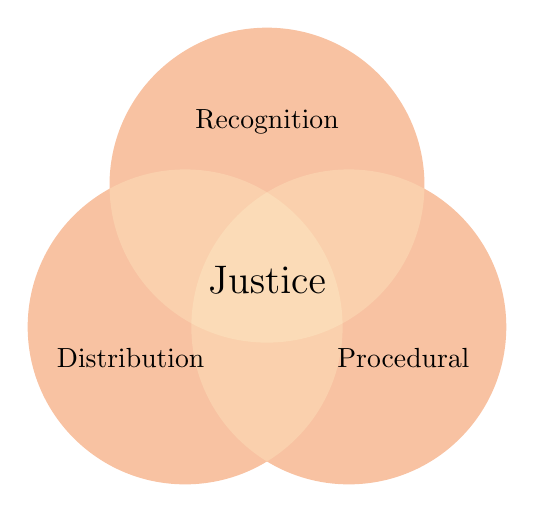
\begin{tikzpicture}
                \begin{scope}[blend group = soft light]
                    % \fill[red!30!white]   ( 90:1.2) circle (2);
                    \fill[illiniorange]   ( 90:1.2) circle (2);
                    % \fill[green!30!white] (210:1.2) circle (2);
                    \fill[illiniorange] (210:1.2) circle (2);
                    % \fill[blue!30!white]  (330:1.2) circle (2);
                    \fill[illiniorange]  (330:1.2) circle (2);
                \end{scope}
                \node at ( 90:2)    {Recognition}; 
                \node at ( 210:2) {Distribution}; 
                \node at ( 330:2)   {Procedural}; 
                \node[font=\Large] {\textcolor{black}{Justice}};
              \end{tikzpicture}

        % }
        \caption{Three aspects of justice \cite{schlosberg_1_2007}.}
    \end{figure}
\end{frame}

\begin{frame}
    \frametitle{\glspl{esom}}
    \Glspl{esom} are a class of tools designed to 
    optimize this transition.
    \\
    % (Provide examples?)

    They will become more important with more \gls{vre}
    and more volatile weather.
    \\\\
    \textit{But they have at least two big flaws}.
    \begin{enumerate}[<+->]
        \item All current \glspl{esom} optimize a single objective --- cost.
        \item \glspl{esom} struggle to model the ``human dimension'' thereby
        limiting their ability to address justice \cite{pfenninger_energy_2014}.
    \end{enumerate}
\end{frame}

\subsection{Introducing \gls{osier}}
\begin{frame}
    \frametitle{\gls{osier}}
    I developed \gls{osier} to fill these gaps by \cite{dotson_osier_2024}
    \begin{enumerate}
        \item optimizing multi- and many-objective problems,
        \item allowing user-defined objectives.
    \end{enumerate}
    
    \begin{figure}
        \centering
        \resizebox{0.95\columnwidth}{!}{%% Creator: Matplotlib, PGF backend
%%
%% To include the figure in your LaTeX document, write
%%   \input{<filename>.pgf}
%%
%% Make sure the required packages are loaded in your preamble
%%   \usepackage{pgf}
%%
%% Also ensure that all the required font packages are loaded; for instance,
%% the lmodern package is sometimes necessary when using math font.
%%   \usepackage{lmodern}
%%
%% Figures using additional raster images can only be included by \input if
%% they are in the same directory as the main LaTeX file. For loading figures
%% from other directories you can use the `import` package
%%   \usepackage{import}
%%
%% and then include the figures with
%%   \import{<path to file>}{<filename>.pgf}
%%
%% Matplotlib used the following preamble
%%   \def\mathdefault#1{#1}
%%   \everymath=\expandafter{\the\everymath\displaystyle}
%%   \IfFileExists{scrextend.sty}{
%%     \usepackage[fontsize=10.000000pt]{scrextend}
%%   }{
%%     \renewcommand{\normalsize}{\fontsize{10.000000}{12.000000}\selectfont}
%%     \normalsize
%%   }
%%   
%%   \makeatletter\@ifpackageloaded{underscore}{}{\usepackage[strings]{underscore}}\makeatother
%%
\begingroup%
\makeatletter%
\begin{pgfpicture}%
\pgfpathrectangle{\pgfpointorigin}{\pgfqpoint{6.600000in}{5.000000in}}%
\pgfusepath{use as bounding box, clip}%
\begin{pgfscope}%
\pgfsetbuttcap%
\pgfsetmiterjoin%
\definecolor{currentfill}{rgb}{1.000000,1.000000,1.000000}%
\pgfsetfillcolor{currentfill}%
\pgfsetlinewidth{0.000000pt}%
\definecolor{currentstroke}{rgb}{0.000000,0.000000,0.000000}%
\pgfsetstrokecolor{currentstroke}%
\pgfsetdash{}{0pt}%
\pgfpathmoveto{\pgfqpoint{0.000000in}{0.000000in}}%
\pgfpathlineto{\pgfqpoint{6.600000in}{0.000000in}}%
\pgfpathlineto{\pgfqpoint{6.600000in}{5.000000in}}%
\pgfpathlineto{\pgfqpoint{0.000000in}{5.000000in}}%
\pgfpathlineto{\pgfqpoint{0.000000in}{0.000000in}}%
\pgfpathclose%
\pgfusepath{fill}%
\end{pgfscope}%
\end{pgfpicture}%
\makeatother%
\endgroup%
}
        \caption{Objective space for a four-objective problem.}
        \label{fig:4-obj-space}
    \end{figure}
\end{frame}

\begin{frame}
    \frametitle{How \gls{osier} Works}

    \begin{figure}
        \centering
        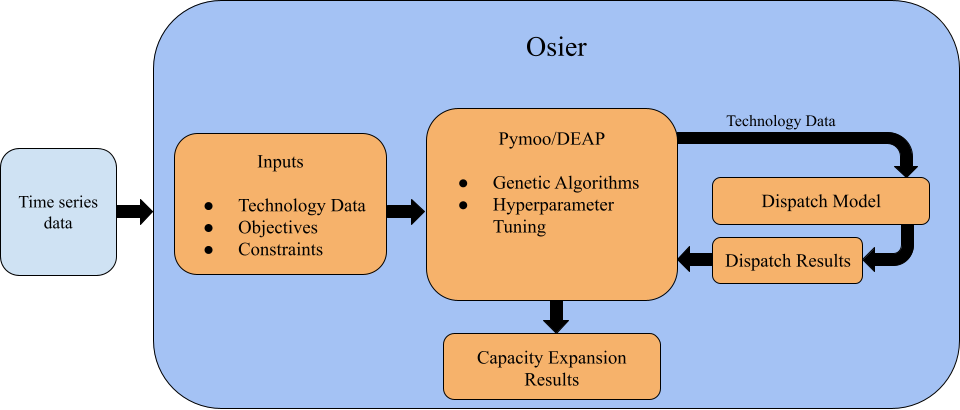
\includegraphics[width=\columnwidth]{../docs/figures/03_osier_chapter/osier_flow.png}
        \caption{Flow of data into and within \gls{osier}}
        \label{fig:osier-flow-1}
    \end{figure}
    % [Show the data flow diagram]

    % Osier works by leveraging genetic algorithsm... 
\end{frame}

\begin{frame}
    \frametitle{Pareto Fronts}
    \begin{figure}
        \centering
        \resizebox{0.75\columnwidth}{!}{%% Creator: Matplotlib, PGF backend
%%
%% To include the figure in your LaTeX document, write
%%   \input{<filename>.pgf}
%%
%% Make sure the required packages are loaded in your preamble
%%   \usepackage{pgf}
%%
%% Also ensure that all the required font packages are loaded; for instance,
%% the lmodern package is sometimes necessary when using math font.
%%   \usepackage{lmodern}
%%
%% Figures using additional raster images can only be included by \input if
%% they are in the same directory as the main LaTeX file. For loading figures
%% from other directories you can use the `import` package
%%   \usepackage{import}
%%
%% and then include the figures with
%%   \import{<path to file>}{<filename>.pgf}
%%
%% Matplotlib used the following preamble
%%   \def\mathdefault#1{#1}
%%   \everymath=\expandafter{\the\everymath\displaystyle}
%%   \IfFileExists{scrextend.sty}{
%%     \usepackage[fontsize=10.000000pt]{scrextend}
%%   }{
%%     \renewcommand{\normalsize}{\fontsize{10.000000}{12.000000}\selectfont}
%%     \normalsize
%%   }
%%   
%%   \makeatletter\@ifpackageloaded{underscore}{}{\usepackage[strings]{underscore}}\makeatother
%%
\begingroup%
\makeatletter%
\begin{pgfpicture}%
\pgfpathrectangle{\pgfpointorigin}{\pgfqpoint{6.869444in}{5.322237in}}%
\pgfusepath{use as bounding box, clip}%
\begin{pgfscope}%
\pgfsetbuttcap%
\pgfsetmiterjoin%
\definecolor{currentfill}{rgb}{1.000000,1.000000,1.000000}%
\pgfsetfillcolor{currentfill}%
\pgfsetlinewidth{0.000000pt}%
\definecolor{currentstroke}{rgb}{0.000000,0.000000,0.000000}%
\pgfsetstrokecolor{currentstroke}%
\pgfsetdash{}{0pt}%
\pgfpathmoveto{\pgfqpoint{0.000000in}{0.000000in}}%
\pgfpathlineto{\pgfqpoint{6.869444in}{0.000000in}}%
\pgfpathlineto{\pgfqpoint{6.869444in}{5.322237in}}%
\pgfpathlineto{\pgfqpoint{0.000000in}{5.322237in}}%
\pgfpathlineto{\pgfqpoint{0.000000in}{0.000000in}}%
\pgfpathclose%
\pgfusepath{fill}%
\end{pgfscope}%
\begin{pgfscope}%
\pgfsetbuttcap%
\pgfsetmiterjoin%
\definecolor{currentfill}{rgb}{1.000000,1.000000,1.000000}%
\pgfsetfillcolor{currentfill}%
\pgfsetlinewidth{0.000000pt}%
\definecolor{currentstroke}{rgb}{0.000000,0.000000,0.000000}%
\pgfsetstrokecolor{currentstroke}%
\pgfsetstrokeopacity{0.000000}%
\pgfsetdash{}{0pt}%
\pgfpathmoveto{\pgfqpoint{0.569444in}{0.554012in}}%
\pgfpathlineto{\pgfqpoint{6.769444in}{0.554012in}}%
\pgfpathlineto{\pgfqpoint{6.769444in}{5.174012in}}%
\pgfpathlineto{\pgfqpoint{0.569444in}{5.174012in}}%
\pgfpathlineto{\pgfqpoint{0.569444in}{0.554012in}}%
\pgfpathclose%
\pgfusepath{fill}%
\end{pgfscope}%
\begin{pgfscope}%
\pgfpathrectangle{\pgfqpoint{0.569444in}{0.554012in}}{\pgfqpoint{6.200000in}{4.620000in}}%
\pgfusepath{clip}%
\pgfsetbuttcap%
\pgfsetroundjoin%
\pgfsetlinewidth{1.003750pt}%
\definecolor{currentstroke}{rgb}{1.000000,0.000000,0.000000}%
\pgfsetstrokecolor{currentstroke}%
\pgfsetdash{}{0pt}%
\pgfpathmoveto{\pgfqpoint{0.569444in}{5.132345in}}%
\pgfpathcurveto{\pgfqpoint{0.580495in}{5.132345in}}{\pgfqpoint{0.591094in}{5.136735in}}{\pgfqpoint{0.598907in}{5.144549in}}%
\pgfpathcurveto{\pgfqpoint{0.606721in}{5.152363in}}{\pgfqpoint{0.611111in}{5.162962in}}{\pgfqpoint{0.611111in}{5.174012in}}%
\pgfpathcurveto{\pgfqpoint{0.611111in}{5.185062in}}{\pgfqpoint{0.606721in}{5.195661in}}{\pgfqpoint{0.598907in}{5.203475in}}%
\pgfpathcurveto{\pgfqpoint{0.591094in}{5.211288in}}{\pgfqpoint{0.580495in}{5.215678in}}{\pgfqpoint{0.569444in}{5.215678in}}%
\pgfpathcurveto{\pgfqpoint{0.558394in}{5.215678in}}{\pgfqpoint{0.547795in}{5.211288in}}{\pgfqpoint{0.539982in}{5.203475in}}%
\pgfpathcurveto{\pgfqpoint{0.532168in}{5.195661in}}{\pgfqpoint{0.527778in}{5.185062in}}{\pgfqpoint{0.527778in}{5.174012in}}%
\pgfpathcurveto{\pgfqpoint{0.527778in}{5.162962in}}{\pgfqpoint{0.532168in}{5.152363in}}{\pgfqpoint{0.539982in}{5.144549in}}%
\pgfpathcurveto{\pgfqpoint{0.547795in}{5.136735in}}{\pgfqpoint{0.558394in}{5.132345in}}{\pgfqpoint{0.569444in}{5.132345in}}%
\pgfpathlineto{\pgfqpoint{0.569444in}{5.132345in}}%
\pgfpathclose%
\pgfusepath{stroke}%
\end{pgfscope}%
\begin{pgfscope}%
\pgfpathrectangle{\pgfqpoint{0.569444in}{0.554012in}}{\pgfqpoint{6.200000in}{4.620000in}}%
\pgfusepath{clip}%
\pgfsetbuttcap%
\pgfsetroundjoin%
\pgfsetlinewidth{1.003750pt}%
\definecolor{currentstroke}{rgb}{1.000000,0.000000,0.000000}%
\pgfsetstrokecolor{currentstroke}%
\pgfsetdash{}{0pt}%
\pgfpathmoveto{\pgfqpoint{0.570375in}{5.031408in}}%
\pgfpathcurveto{\pgfqpoint{0.581425in}{5.031408in}}{\pgfqpoint{0.592024in}{5.035798in}}{\pgfqpoint{0.599838in}{5.043612in}}%
\pgfpathcurveto{\pgfqpoint{0.607651in}{5.051426in}}{\pgfqpoint{0.612041in}{5.062025in}}{\pgfqpoint{0.612041in}{5.073075in}}%
\pgfpathcurveto{\pgfqpoint{0.612041in}{5.084125in}}{\pgfqpoint{0.607651in}{5.094724in}}{\pgfqpoint{0.599838in}{5.102538in}}%
\pgfpathcurveto{\pgfqpoint{0.592024in}{5.110351in}}{\pgfqpoint{0.581425in}{5.114742in}}{\pgfqpoint{0.570375in}{5.114742in}}%
\pgfpathcurveto{\pgfqpoint{0.559325in}{5.114742in}}{\pgfqpoint{0.548726in}{5.110351in}}{\pgfqpoint{0.540912in}{5.102538in}}%
\pgfpathcurveto{\pgfqpoint{0.533098in}{5.094724in}}{\pgfqpoint{0.528708in}{5.084125in}}{\pgfqpoint{0.528708in}{5.073075in}}%
\pgfpathcurveto{\pgfqpoint{0.528708in}{5.062025in}}{\pgfqpoint{0.533098in}{5.051426in}}{\pgfqpoint{0.540912in}{5.043612in}}%
\pgfpathcurveto{\pgfqpoint{0.548726in}{5.035798in}}{\pgfqpoint{0.559325in}{5.031408in}}{\pgfqpoint{0.570375in}{5.031408in}}%
\pgfpathlineto{\pgfqpoint{0.570375in}{5.031408in}}%
\pgfpathclose%
\pgfusepath{stroke}%
\end{pgfscope}%
\begin{pgfscope}%
\pgfpathrectangle{\pgfqpoint{0.569444in}{0.554012in}}{\pgfqpoint{6.200000in}{4.620000in}}%
\pgfusepath{clip}%
\pgfsetbuttcap%
\pgfsetroundjoin%
\pgfsetlinewidth{1.003750pt}%
\definecolor{currentstroke}{rgb}{1.000000,0.000000,0.000000}%
\pgfsetstrokecolor{currentstroke}%
\pgfsetdash{}{0pt}%
\pgfpathmoveto{\pgfqpoint{0.573166in}{4.931496in}}%
\pgfpathcurveto{\pgfqpoint{0.584216in}{4.931496in}}{\pgfqpoint{0.594815in}{4.935886in}}{\pgfqpoint{0.602628in}{4.943700in}}%
\pgfpathcurveto{\pgfqpoint{0.610442in}{4.951514in}}{\pgfqpoint{0.614832in}{4.962113in}}{\pgfqpoint{0.614832in}{4.973163in}}%
\pgfpathcurveto{\pgfqpoint{0.614832in}{4.984213in}}{\pgfqpoint{0.610442in}{4.994812in}}{\pgfqpoint{0.602628in}{5.002626in}}%
\pgfpathcurveto{\pgfqpoint{0.594815in}{5.010439in}}{\pgfqpoint{0.584216in}{5.014829in}}{\pgfqpoint{0.573166in}{5.014829in}}%
\pgfpathcurveto{\pgfqpoint{0.562115in}{5.014829in}}{\pgfqpoint{0.551516in}{5.010439in}}{\pgfqpoint{0.543703in}{5.002626in}}%
\pgfpathcurveto{\pgfqpoint{0.535889in}{4.994812in}}{\pgfqpoint{0.531499in}{4.984213in}}{\pgfqpoint{0.531499in}{4.973163in}}%
\pgfpathcurveto{\pgfqpoint{0.531499in}{4.962113in}}{\pgfqpoint{0.535889in}{4.951514in}}{\pgfqpoint{0.543703in}{4.943700in}}%
\pgfpathcurveto{\pgfqpoint{0.551516in}{4.935886in}}{\pgfqpoint{0.562115in}{4.931496in}}{\pgfqpoint{0.573166in}{4.931496in}}%
\pgfpathlineto{\pgfqpoint{0.573166in}{4.931496in}}%
\pgfpathclose%
\pgfusepath{stroke}%
\end{pgfscope}%
\begin{pgfscope}%
\pgfpathrectangle{\pgfqpoint{0.569444in}{0.554012in}}{\pgfqpoint{6.200000in}{4.620000in}}%
\pgfusepath{clip}%
\pgfsetbuttcap%
\pgfsetroundjoin%
\pgfsetlinewidth{1.003750pt}%
\definecolor{currentstroke}{rgb}{1.000000,0.000000,0.000000}%
\pgfsetstrokecolor{currentstroke}%
\pgfsetdash{}{0pt}%
\pgfpathmoveto{\pgfqpoint{0.577817in}{4.832609in}}%
\pgfpathcurveto{\pgfqpoint{0.588867in}{4.832609in}}{\pgfqpoint{0.599466in}{4.836999in}}{\pgfqpoint{0.607280in}{4.844813in}}%
\pgfpathcurveto{\pgfqpoint{0.615093in}{4.852626in}}{\pgfqpoint{0.619484in}{4.863225in}}{\pgfqpoint{0.619484in}{4.874275in}}%
\pgfpathcurveto{\pgfqpoint{0.619484in}{4.885325in}}{\pgfqpoint{0.615093in}{4.895924in}}{\pgfqpoint{0.607280in}{4.903738in}}%
\pgfpathcurveto{\pgfqpoint{0.599466in}{4.911552in}}{\pgfqpoint{0.588867in}{4.915942in}}{\pgfqpoint{0.577817in}{4.915942in}}%
\pgfpathcurveto{\pgfqpoint{0.566767in}{4.915942in}}{\pgfqpoint{0.556168in}{4.911552in}}{\pgfqpoint{0.548354in}{4.903738in}}%
\pgfpathcurveto{\pgfqpoint{0.540541in}{4.895924in}}{\pgfqpoint{0.536150in}{4.885325in}}{\pgfqpoint{0.536150in}{4.874275in}}%
\pgfpathcurveto{\pgfqpoint{0.536150in}{4.863225in}}{\pgfqpoint{0.540541in}{4.852626in}}{\pgfqpoint{0.548354in}{4.844813in}}%
\pgfpathcurveto{\pgfqpoint{0.556168in}{4.836999in}}{\pgfqpoint{0.566767in}{4.832609in}}{\pgfqpoint{0.577817in}{4.832609in}}%
\pgfpathlineto{\pgfqpoint{0.577817in}{4.832609in}}%
\pgfpathclose%
\pgfusepath{stroke}%
\end{pgfscope}%
\begin{pgfscope}%
\pgfpathrectangle{\pgfqpoint{0.569444in}{0.554012in}}{\pgfqpoint{6.200000in}{4.620000in}}%
\pgfusepath{clip}%
\pgfsetbuttcap%
\pgfsetroundjoin%
\pgfsetlinewidth{1.003750pt}%
\definecolor{currentstroke}{rgb}{1.000000,0.000000,0.000000}%
\pgfsetstrokecolor{currentstroke}%
\pgfsetdash{}{0pt}%
\pgfpathmoveto{\pgfqpoint{0.584329in}{4.734746in}}%
\pgfpathcurveto{\pgfqpoint{0.595379in}{4.734746in}}{\pgfqpoint{0.605978in}{4.739136in}}{\pgfqpoint{0.613792in}{4.746950in}}%
\pgfpathcurveto{\pgfqpoint{0.621605in}{4.754763in}}{\pgfqpoint{0.625996in}{4.765362in}}{\pgfqpoint{0.625996in}{4.776413in}}%
\pgfpathcurveto{\pgfqpoint{0.625996in}{4.787463in}}{\pgfqpoint{0.621605in}{4.798062in}}{\pgfqpoint{0.613792in}{4.805875in}}%
\pgfpathcurveto{\pgfqpoint{0.605978in}{4.813689in}}{\pgfqpoint{0.595379in}{4.818079in}}{\pgfqpoint{0.584329in}{4.818079in}}%
\pgfpathcurveto{\pgfqpoint{0.573279in}{4.818079in}}{\pgfqpoint{0.562680in}{4.813689in}}{\pgfqpoint{0.554866in}{4.805875in}}%
\pgfpathcurveto{\pgfqpoint{0.547052in}{4.798062in}}{\pgfqpoint{0.542662in}{4.787463in}}{\pgfqpoint{0.542662in}{4.776413in}}%
\pgfpathcurveto{\pgfqpoint{0.542662in}{4.765362in}}{\pgfqpoint{0.547052in}{4.754763in}}{\pgfqpoint{0.554866in}{4.746950in}}%
\pgfpathcurveto{\pgfqpoint{0.562680in}{4.739136in}}{\pgfqpoint{0.573279in}{4.734746in}}{\pgfqpoint{0.584329in}{4.734746in}}%
\pgfpathlineto{\pgfqpoint{0.584329in}{4.734746in}}%
\pgfpathclose%
\pgfusepath{stroke}%
\end{pgfscope}%
\begin{pgfscope}%
\pgfpathrectangle{\pgfqpoint{0.569444in}{0.554012in}}{\pgfqpoint{6.200000in}{4.620000in}}%
\pgfusepath{clip}%
\pgfsetbuttcap%
\pgfsetroundjoin%
\pgfsetlinewidth{1.003750pt}%
\definecolor{currentstroke}{rgb}{1.000000,0.000000,0.000000}%
\pgfsetstrokecolor{currentstroke}%
\pgfsetdash{}{0pt}%
\pgfpathmoveto{\pgfqpoint{0.592701in}{4.637908in}}%
\pgfpathcurveto{\pgfqpoint{0.603752in}{4.637908in}}{\pgfqpoint{0.614351in}{4.642298in}}{\pgfqpoint{0.622164in}{4.650112in}}%
\pgfpathcurveto{\pgfqpoint{0.629978in}{4.657926in}}{\pgfqpoint{0.634368in}{4.668525in}}{\pgfqpoint{0.634368in}{4.679575in}}%
\pgfpathcurveto{\pgfqpoint{0.634368in}{4.690625in}}{\pgfqpoint{0.629978in}{4.701224in}}{\pgfqpoint{0.622164in}{4.709037in}}%
\pgfpathcurveto{\pgfqpoint{0.614351in}{4.716851in}}{\pgfqpoint{0.603752in}{4.721241in}}{\pgfqpoint{0.592701in}{4.721241in}}%
\pgfpathcurveto{\pgfqpoint{0.581651in}{4.721241in}}{\pgfqpoint{0.571052in}{4.716851in}}{\pgfqpoint{0.563239in}{4.709037in}}%
\pgfpathcurveto{\pgfqpoint{0.555425in}{4.701224in}}{\pgfqpoint{0.551035in}{4.690625in}}{\pgfqpoint{0.551035in}{4.679575in}}%
\pgfpathcurveto{\pgfqpoint{0.551035in}{4.668525in}}{\pgfqpoint{0.555425in}{4.657926in}}{\pgfqpoint{0.563239in}{4.650112in}}%
\pgfpathcurveto{\pgfqpoint{0.571052in}{4.642298in}}{\pgfqpoint{0.581651in}{4.637908in}}{\pgfqpoint{0.592701in}{4.637908in}}%
\pgfpathlineto{\pgfqpoint{0.592701in}{4.637908in}}%
\pgfpathclose%
\pgfusepath{stroke}%
\end{pgfscope}%
\begin{pgfscope}%
\pgfpathrectangle{\pgfqpoint{0.569444in}{0.554012in}}{\pgfqpoint{6.200000in}{4.620000in}}%
\pgfusepath{clip}%
\pgfsetbuttcap%
\pgfsetroundjoin%
\pgfsetlinewidth{1.003750pt}%
\definecolor{currentstroke}{rgb}{1.000000,0.000000,0.000000}%
\pgfsetstrokecolor{currentstroke}%
\pgfsetdash{}{0pt}%
\pgfpathmoveto{\pgfqpoint{0.602934in}{4.542095in}}%
\pgfpathcurveto{\pgfqpoint{0.613985in}{4.542095in}}{\pgfqpoint{0.624584in}{4.546485in}}{\pgfqpoint{0.632397in}{4.554299in}}%
\pgfpathcurveto{\pgfqpoint{0.640211in}{4.562112in}}{\pgfqpoint{0.644601in}{4.572711in}}{\pgfqpoint{0.644601in}{4.583761in}}%
\pgfpathcurveto{\pgfqpoint{0.644601in}{4.594812in}}{\pgfqpoint{0.640211in}{4.605411in}}{\pgfqpoint{0.632397in}{4.613224in}}%
\pgfpathcurveto{\pgfqpoint{0.624584in}{4.621038in}}{\pgfqpoint{0.613985in}{4.625428in}}{\pgfqpoint{0.602934in}{4.625428in}}%
\pgfpathcurveto{\pgfqpoint{0.591884in}{4.625428in}}{\pgfqpoint{0.581285in}{4.621038in}}{\pgfqpoint{0.573472in}{4.613224in}}%
\pgfpathcurveto{\pgfqpoint{0.565658in}{4.605411in}}{\pgfqpoint{0.561268in}{4.594812in}}{\pgfqpoint{0.561268in}{4.583761in}}%
\pgfpathcurveto{\pgfqpoint{0.561268in}{4.572711in}}{\pgfqpoint{0.565658in}{4.562112in}}{\pgfqpoint{0.573472in}{4.554299in}}%
\pgfpathcurveto{\pgfqpoint{0.581285in}{4.546485in}}{\pgfqpoint{0.591884in}{4.542095in}}{\pgfqpoint{0.602934in}{4.542095in}}%
\pgfpathlineto{\pgfqpoint{0.602934in}{4.542095in}}%
\pgfpathclose%
\pgfusepath{stroke}%
\end{pgfscope}%
\begin{pgfscope}%
\pgfpathrectangle{\pgfqpoint{0.569444in}{0.554012in}}{\pgfqpoint{6.200000in}{4.620000in}}%
\pgfusepath{clip}%
\pgfsetbuttcap%
\pgfsetroundjoin%
\pgfsetlinewidth{1.003750pt}%
\definecolor{currentstroke}{rgb}{1.000000,0.000000,0.000000}%
\pgfsetstrokecolor{currentstroke}%
\pgfsetdash{}{0pt}%
\pgfpathmoveto{\pgfqpoint{0.615028in}{4.447306in}}%
\pgfpathcurveto{\pgfqpoint{0.626078in}{4.447306in}}{\pgfqpoint{0.636677in}{4.451697in}}{\pgfqpoint{0.644491in}{4.459510in}}%
\pgfpathcurveto{\pgfqpoint{0.652304in}{4.467324in}}{\pgfqpoint{0.656695in}{4.477923in}}{\pgfqpoint{0.656695in}{4.488973in}}%
\pgfpathcurveto{\pgfqpoint{0.656695in}{4.500023in}}{\pgfqpoint{0.652304in}{4.510622in}}{\pgfqpoint{0.644491in}{4.518436in}}%
\pgfpathcurveto{\pgfqpoint{0.636677in}{4.526249in}}{\pgfqpoint{0.626078in}{4.530640in}}{\pgfqpoint{0.615028in}{4.530640in}}%
\pgfpathcurveto{\pgfqpoint{0.603978in}{4.530640in}}{\pgfqpoint{0.593379in}{4.526249in}}{\pgfqpoint{0.585565in}{4.518436in}}%
\pgfpathcurveto{\pgfqpoint{0.577752in}{4.510622in}}{\pgfqpoint{0.573361in}{4.500023in}}{\pgfqpoint{0.573361in}{4.488973in}}%
\pgfpathcurveto{\pgfqpoint{0.573361in}{4.477923in}}{\pgfqpoint{0.577752in}{4.467324in}}{\pgfqpoint{0.585565in}{4.459510in}}%
\pgfpathcurveto{\pgfqpoint{0.593379in}{4.451697in}}{\pgfqpoint{0.603978in}{4.447306in}}{\pgfqpoint{0.615028in}{4.447306in}}%
\pgfpathlineto{\pgfqpoint{0.615028in}{4.447306in}}%
\pgfpathclose%
\pgfusepath{stroke}%
\end{pgfscope}%
\begin{pgfscope}%
\pgfpathrectangle{\pgfqpoint{0.569444in}{0.554012in}}{\pgfqpoint{6.200000in}{4.620000in}}%
\pgfusepath{clip}%
\pgfsetbuttcap%
\pgfsetroundjoin%
\pgfsetlinewidth{1.003750pt}%
\definecolor{currentstroke}{rgb}{1.000000,0.000000,0.000000}%
\pgfsetstrokecolor{currentstroke}%
\pgfsetdash{}{0pt}%
\pgfpathmoveto{\pgfqpoint{0.628982in}{4.353543in}}%
\pgfpathcurveto{\pgfqpoint{0.640032in}{4.353543in}}{\pgfqpoint{0.650631in}{4.357933in}}{\pgfqpoint{0.658445in}{4.365747in}}%
\pgfpathcurveto{\pgfqpoint{0.666259in}{4.373560in}}{\pgfqpoint{0.670649in}{4.384159in}}{\pgfqpoint{0.670649in}{4.395209in}}%
\pgfpathcurveto{\pgfqpoint{0.670649in}{4.406259in}}{\pgfqpoint{0.666259in}{4.416858in}}{\pgfqpoint{0.658445in}{4.424672in}}%
\pgfpathcurveto{\pgfqpoint{0.650631in}{4.432486in}}{\pgfqpoint{0.640032in}{4.436876in}}{\pgfqpoint{0.628982in}{4.436876in}}%
\pgfpathcurveto{\pgfqpoint{0.617932in}{4.436876in}}{\pgfqpoint{0.607333in}{4.432486in}}{\pgfqpoint{0.599519in}{4.424672in}}%
\pgfpathcurveto{\pgfqpoint{0.591706in}{4.416858in}}{\pgfqpoint{0.587316in}{4.406259in}}{\pgfqpoint{0.587316in}{4.395209in}}%
\pgfpathcurveto{\pgfqpoint{0.587316in}{4.384159in}}{\pgfqpoint{0.591706in}{4.373560in}}{\pgfqpoint{0.599519in}{4.365747in}}%
\pgfpathcurveto{\pgfqpoint{0.607333in}{4.357933in}}{\pgfqpoint{0.617932in}{4.353543in}}{\pgfqpoint{0.628982in}{4.353543in}}%
\pgfpathlineto{\pgfqpoint{0.628982in}{4.353543in}}%
\pgfpathclose%
\pgfusepath{stroke}%
\end{pgfscope}%
\begin{pgfscope}%
\pgfpathrectangle{\pgfqpoint{0.569444in}{0.554012in}}{\pgfqpoint{6.200000in}{4.620000in}}%
\pgfusepath{clip}%
\pgfsetbuttcap%
\pgfsetroundjoin%
\pgfsetlinewidth{1.003750pt}%
\definecolor{currentstroke}{rgb}{1.000000,0.000000,0.000000}%
\pgfsetstrokecolor{currentstroke}%
\pgfsetdash{}{0pt}%
\pgfpathmoveto{\pgfqpoint{0.644797in}{4.260804in}}%
\pgfpathcurveto{\pgfqpoint{0.655847in}{4.260804in}}{\pgfqpoint{0.666446in}{4.265194in}}{\pgfqpoint{0.674260in}{4.273008in}}%
\pgfpathcurveto{\pgfqpoint{0.682073in}{4.280821in}}{\pgfqpoint{0.686464in}{4.291420in}}{\pgfqpoint{0.686464in}{4.302470in}}%
\pgfpathcurveto{\pgfqpoint{0.686464in}{4.313520in}}{\pgfqpoint{0.682073in}{4.324119in}}{\pgfqpoint{0.674260in}{4.331933in}}%
\pgfpathcurveto{\pgfqpoint{0.666446in}{4.339747in}}{\pgfqpoint{0.655847in}{4.344137in}}{\pgfqpoint{0.644797in}{4.344137in}}%
\pgfpathcurveto{\pgfqpoint{0.633747in}{4.344137in}}{\pgfqpoint{0.623148in}{4.339747in}}{\pgfqpoint{0.615334in}{4.331933in}}%
\pgfpathcurveto{\pgfqpoint{0.607520in}{4.324119in}}{\pgfqpoint{0.603130in}{4.313520in}}{\pgfqpoint{0.603130in}{4.302470in}}%
\pgfpathcurveto{\pgfqpoint{0.603130in}{4.291420in}}{\pgfqpoint{0.607520in}{4.280821in}}{\pgfqpoint{0.615334in}{4.273008in}}%
\pgfpathcurveto{\pgfqpoint{0.623148in}{4.265194in}}{\pgfqpoint{0.633747in}{4.260804in}}{\pgfqpoint{0.644797in}{4.260804in}}%
\pgfpathlineto{\pgfqpoint{0.644797in}{4.260804in}}%
\pgfpathclose%
\pgfusepath{stroke}%
\end{pgfscope}%
\begin{pgfscope}%
\pgfpathrectangle{\pgfqpoint{0.569444in}{0.554012in}}{\pgfqpoint{6.200000in}{4.620000in}}%
\pgfusepath{clip}%
\pgfsetbuttcap%
\pgfsetroundjoin%
\pgfsetlinewidth{1.003750pt}%
\definecolor{currentstroke}{rgb}{1.000000,0.000000,0.000000}%
\pgfsetstrokecolor{currentstroke}%
\pgfsetdash{}{0pt}%
\pgfpathmoveto{\pgfqpoint{0.662472in}{4.169089in}}%
\pgfpathcurveto{\pgfqpoint{0.673522in}{4.169089in}}{\pgfqpoint{0.684121in}{4.173480in}}{\pgfqpoint{0.691935in}{4.181293in}}%
\pgfpathcurveto{\pgfqpoint{0.699749in}{4.189107in}}{\pgfqpoint{0.704139in}{4.199706in}}{\pgfqpoint{0.704139in}{4.210756in}}%
\pgfpathcurveto{\pgfqpoint{0.704139in}{4.221806in}}{\pgfqpoint{0.699749in}{4.232405in}}{\pgfqpoint{0.691935in}{4.240219in}}%
\pgfpathcurveto{\pgfqpoint{0.684121in}{4.248032in}}{\pgfqpoint{0.673522in}{4.252423in}}{\pgfqpoint{0.662472in}{4.252423in}}%
\pgfpathcurveto{\pgfqpoint{0.651422in}{4.252423in}}{\pgfqpoint{0.640823in}{4.248032in}}{\pgfqpoint{0.633009in}{4.240219in}}%
\pgfpathcurveto{\pgfqpoint{0.625196in}{4.232405in}}{\pgfqpoint{0.620806in}{4.221806in}}{\pgfqpoint{0.620806in}{4.210756in}}%
\pgfpathcurveto{\pgfqpoint{0.620806in}{4.199706in}}{\pgfqpoint{0.625196in}{4.189107in}}{\pgfqpoint{0.633009in}{4.181293in}}%
\pgfpathcurveto{\pgfqpoint{0.640823in}{4.173480in}}{\pgfqpoint{0.651422in}{4.169089in}}{\pgfqpoint{0.662472in}{4.169089in}}%
\pgfpathlineto{\pgfqpoint{0.662472in}{4.169089in}}%
\pgfpathclose%
\pgfusepath{stroke}%
\end{pgfscope}%
\begin{pgfscope}%
\pgfpathrectangle{\pgfqpoint{0.569444in}{0.554012in}}{\pgfqpoint{6.200000in}{4.620000in}}%
\pgfusepath{clip}%
\pgfsetbuttcap%
\pgfsetroundjoin%
\pgfsetlinewidth{1.003750pt}%
\definecolor{currentstroke}{rgb}{1.000000,0.000000,0.000000}%
\pgfsetstrokecolor{currentstroke}%
\pgfsetdash{}{0pt}%
\pgfpathmoveto{\pgfqpoint{0.682008in}{4.078400in}}%
\pgfpathcurveto{\pgfqpoint{0.693058in}{4.078400in}}{\pgfqpoint{0.703657in}{4.082790in}}{\pgfqpoint{0.711471in}{4.090604in}}%
\pgfpathcurveto{\pgfqpoint{0.719284in}{4.098417in}}{\pgfqpoint{0.723675in}{4.109016in}}{\pgfqpoint{0.723675in}{4.120067in}}%
\pgfpathcurveto{\pgfqpoint{0.723675in}{4.131117in}}{\pgfqpoint{0.719284in}{4.141716in}}{\pgfqpoint{0.711471in}{4.149529in}}%
\pgfpathcurveto{\pgfqpoint{0.703657in}{4.157343in}}{\pgfqpoint{0.693058in}{4.161733in}}{\pgfqpoint{0.682008in}{4.161733in}}%
\pgfpathcurveto{\pgfqpoint{0.670958in}{4.161733in}}{\pgfqpoint{0.660359in}{4.157343in}}{\pgfqpoint{0.652545in}{4.149529in}}%
\pgfpathcurveto{\pgfqpoint{0.644732in}{4.141716in}}{\pgfqpoint{0.640341in}{4.131117in}}{\pgfqpoint{0.640341in}{4.120067in}}%
\pgfpathcurveto{\pgfqpoint{0.640341in}{4.109016in}}{\pgfqpoint{0.644732in}{4.098417in}}{\pgfqpoint{0.652545in}{4.090604in}}%
\pgfpathcurveto{\pgfqpoint{0.660359in}{4.082790in}}{\pgfqpoint{0.670958in}{4.078400in}}{\pgfqpoint{0.682008in}{4.078400in}}%
\pgfpathlineto{\pgfqpoint{0.682008in}{4.078400in}}%
\pgfpathclose%
\pgfusepath{stroke}%
\end{pgfscope}%
\begin{pgfscope}%
\pgfpathrectangle{\pgfqpoint{0.569444in}{0.554012in}}{\pgfqpoint{6.200000in}{4.620000in}}%
\pgfusepath{clip}%
\pgfsetbuttcap%
\pgfsetroundjoin%
\pgfsetlinewidth{1.003750pt}%
\definecolor{currentstroke}{rgb}{1.000000,0.000000,0.000000}%
\pgfsetstrokecolor{currentstroke}%
\pgfsetdash{}{0pt}%
\pgfpathmoveto{\pgfqpoint{0.703404in}{3.988735in}}%
\pgfpathcurveto{\pgfqpoint{0.714454in}{3.988735in}}{\pgfqpoint{0.725054in}{3.993125in}}{\pgfqpoint{0.732867in}{4.000939in}}%
\pgfpathcurveto{\pgfqpoint{0.740681in}{4.008753in}}{\pgfqpoint{0.745071in}{4.019352in}}{\pgfqpoint{0.745071in}{4.030402in}}%
\pgfpathcurveto{\pgfqpoint{0.745071in}{4.041452in}}{\pgfqpoint{0.740681in}{4.052051in}}{\pgfqpoint{0.732867in}{4.059865in}}%
\pgfpathcurveto{\pgfqpoint{0.725054in}{4.067678in}}{\pgfqpoint{0.714454in}{4.072068in}}{\pgfqpoint{0.703404in}{4.072068in}}%
\pgfpathcurveto{\pgfqpoint{0.692354in}{4.072068in}}{\pgfqpoint{0.681755in}{4.067678in}}{\pgfqpoint{0.673942in}{4.059865in}}%
\pgfpathcurveto{\pgfqpoint{0.666128in}{4.052051in}}{\pgfqpoint{0.661738in}{4.041452in}}{\pgfqpoint{0.661738in}{4.030402in}}%
\pgfpathcurveto{\pgfqpoint{0.661738in}{4.019352in}}{\pgfqpoint{0.666128in}{4.008753in}}{\pgfqpoint{0.673942in}{4.000939in}}%
\pgfpathcurveto{\pgfqpoint{0.681755in}{3.993125in}}{\pgfqpoint{0.692354in}{3.988735in}}{\pgfqpoint{0.703404in}{3.988735in}}%
\pgfpathlineto{\pgfqpoint{0.703404in}{3.988735in}}%
\pgfpathclose%
\pgfusepath{stroke}%
\end{pgfscope}%
\begin{pgfscope}%
\pgfpathrectangle{\pgfqpoint{0.569444in}{0.554012in}}{\pgfqpoint{6.200000in}{4.620000in}}%
\pgfusepath{clip}%
\pgfsetbuttcap%
\pgfsetroundjoin%
\pgfsetlinewidth{1.003750pt}%
\definecolor{currentstroke}{rgb}{1.000000,0.000000,0.000000}%
\pgfsetstrokecolor{currentstroke}%
\pgfsetdash{}{0pt}%
\pgfpathmoveto{\pgfqpoint{0.726661in}{3.900095in}}%
\pgfpathcurveto{\pgfqpoint{0.737711in}{3.900095in}}{\pgfqpoint{0.748310in}{3.904485in}}{\pgfqpoint{0.756124in}{3.912299in}}%
\pgfpathcurveto{\pgfqpoint{0.763938in}{3.920113in}}{\pgfqpoint{0.768328in}{3.930712in}}{\pgfqpoint{0.768328in}{3.941762in}}%
\pgfpathcurveto{\pgfqpoint{0.768328in}{3.952812in}}{\pgfqpoint{0.763938in}{3.963411in}}{\pgfqpoint{0.756124in}{3.971225in}}%
\pgfpathcurveto{\pgfqpoint{0.748310in}{3.979038in}}{\pgfqpoint{0.737711in}{3.983428in}}{\pgfqpoint{0.726661in}{3.983428in}}%
\pgfpathcurveto{\pgfqpoint{0.715611in}{3.983428in}}{\pgfqpoint{0.705012in}{3.979038in}}{\pgfqpoint{0.697199in}{3.971225in}}%
\pgfpathcurveto{\pgfqpoint{0.689385in}{3.963411in}}{\pgfqpoint{0.684995in}{3.952812in}}{\pgfqpoint{0.684995in}{3.941762in}}%
\pgfpathcurveto{\pgfqpoint{0.684995in}{3.930712in}}{\pgfqpoint{0.689385in}{3.920113in}}{\pgfqpoint{0.697199in}{3.912299in}}%
\pgfpathcurveto{\pgfqpoint{0.705012in}{3.904485in}}{\pgfqpoint{0.715611in}{3.900095in}}{\pgfqpoint{0.726661in}{3.900095in}}%
\pgfpathlineto{\pgfqpoint{0.726661in}{3.900095in}}%
\pgfpathclose%
\pgfusepath{stroke}%
\end{pgfscope}%
\begin{pgfscope}%
\pgfpathrectangle{\pgfqpoint{0.569444in}{0.554012in}}{\pgfqpoint{6.200000in}{4.620000in}}%
\pgfusepath{clip}%
\pgfsetbuttcap%
\pgfsetroundjoin%
\pgfsetlinewidth{1.003750pt}%
\definecolor{currentstroke}{rgb}{1.000000,0.000000,0.000000}%
\pgfsetstrokecolor{currentstroke}%
\pgfsetdash{}{0pt}%
\pgfpathmoveto{\pgfqpoint{0.751779in}{3.812480in}}%
\pgfpathcurveto{\pgfqpoint{0.762829in}{3.812480in}}{\pgfqpoint{0.773428in}{3.816870in}}{\pgfqpoint{0.781242in}{3.824684in}}%
\pgfpathcurveto{\pgfqpoint{0.789055in}{3.832497in}}{\pgfqpoint{0.793445in}{3.843096in}}{\pgfqpoint{0.793445in}{3.854146in}}%
\pgfpathcurveto{\pgfqpoint{0.793445in}{3.865197in}}{\pgfqpoint{0.789055in}{3.875796in}}{\pgfqpoint{0.781242in}{3.883609in}}%
\pgfpathcurveto{\pgfqpoint{0.773428in}{3.891423in}}{\pgfqpoint{0.762829in}{3.895813in}}{\pgfqpoint{0.751779in}{3.895813in}}%
\pgfpathcurveto{\pgfqpoint{0.740729in}{3.895813in}}{\pgfqpoint{0.730130in}{3.891423in}}{\pgfqpoint{0.722316in}{3.883609in}}%
\pgfpathcurveto{\pgfqpoint{0.714502in}{3.875796in}}{\pgfqpoint{0.710112in}{3.865197in}}{\pgfqpoint{0.710112in}{3.854146in}}%
\pgfpathcurveto{\pgfqpoint{0.710112in}{3.843096in}}{\pgfqpoint{0.714502in}{3.832497in}}{\pgfqpoint{0.722316in}{3.824684in}}%
\pgfpathcurveto{\pgfqpoint{0.730130in}{3.816870in}}{\pgfqpoint{0.740729in}{3.812480in}}{\pgfqpoint{0.751779in}{3.812480in}}%
\pgfpathlineto{\pgfqpoint{0.751779in}{3.812480in}}%
\pgfpathclose%
\pgfusepath{stroke}%
\end{pgfscope}%
\begin{pgfscope}%
\pgfpathrectangle{\pgfqpoint{0.569444in}{0.554012in}}{\pgfqpoint{6.200000in}{4.620000in}}%
\pgfusepath{clip}%
\pgfsetbuttcap%
\pgfsetroundjoin%
\pgfsetlinewidth{1.003750pt}%
\definecolor{currentstroke}{rgb}{1.000000,0.000000,0.000000}%
\pgfsetstrokecolor{currentstroke}%
\pgfsetdash{}{0pt}%
\pgfpathmoveto{\pgfqpoint{0.778757in}{3.725889in}}%
\pgfpathcurveto{\pgfqpoint{0.789807in}{3.725889in}}{\pgfqpoint{0.800406in}{3.730280in}}{\pgfqpoint{0.808220in}{3.738093in}}%
\pgfpathcurveto{\pgfqpoint{0.816033in}{3.745907in}}{\pgfqpoint{0.820423in}{3.756506in}}{\pgfqpoint{0.820423in}{3.767556in}}%
\pgfpathcurveto{\pgfqpoint{0.820423in}{3.778606in}}{\pgfqpoint{0.816033in}{3.789205in}}{\pgfqpoint{0.808220in}{3.797019in}}%
\pgfpathcurveto{\pgfqpoint{0.800406in}{3.804832in}}{\pgfqpoint{0.789807in}{3.809223in}}{\pgfqpoint{0.778757in}{3.809223in}}%
\pgfpathcurveto{\pgfqpoint{0.767707in}{3.809223in}}{\pgfqpoint{0.757108in}{3.804832in}}{\pgfqpoint{0.749294in}{3.797019in}}%
\pgfpathcurveto{\pgfqpoint{0.741480in}{3.789205in}}{\pgfqpoint{0.737090in}{3.778606in}}{\pgfqpoint{0.737090in}{3.767556in}}%
\pgfpathcurveto{\pgfqpoint{0.737090in}{3.756506in}}{\pgfqpoint{0.741480in}{3.745907in}}{\pgfqpoint{0.749294in}{3.738093in}}%
\pgfpathcurveto{\pgfqpoint{0.757108in}{3.730280in}}{\pgfqpoint{0.767707in}{3.725889in}}{\pgfqpoint{0.778757in}{3.725889in}}%
\pgfpathlineto{\pgfqpoint{0.778757in}{3.725889in}}%
\pgfpathclose%
\pgfusepath{stroke}%
\end{pgfscope}%
\begin{pgfscope}%
\pgfpathrectangle{\pgfqpoint{0.569444in}{0.554012in}}{\pgfqpoint{6.200000in}{4.620000in}}%
\pgfusepath{clip}%
\pgfsetbuttcap%
\pgfsetroundjoin%
\pgfsetlinewidth{1.003750pt}%
\definecolor{currentstroke}{rgb}{1.000000,0.000000,0.000000}%
\pgfsetstrokecolor{currentstroke}%
\pgfsetdash{}{0pt}%
\pgfpathmoveto{\pgfqpoint{0.807595in}{3.640323in}}%
\pgfpathcurveto{\pgfqpoint{0.818646in}{3.640323in}}{\pgfqpoint{0.829245in}{3.644714in}}{\pgfqpoint{0.837058in}{3.652527in}}%
\pgfpathcurveto{\pgfqpoint{0.844872in}{3.660341in}}{\pgfqpoint{0.849262in}{3.670940in}}{\pgfqpoint{0.849262in}{3.681990in}}%
\pgfpathcurveto{\pgfqpoint{0.849262in}{3.693040in}}{\pgfqpoint{0.844872in}{3.703639in}}{\pgfqpoint{0.837058in}{3.711453in}}%
\pgfpathcurveto{\pgfqpoint{0.829245in}{3.719267in}}{\pgfqpoint{0.818646in}{3.723657in}}{\pgfqpoint{0.807595in}{3.723657in}}%
\pgfpathcurveto{\pgfqpoint{0.796545in}{3.723657in}}{\pgfqpoint{0.785946in}{3.719267in}}{\pgfqpoint{0.778133in}{3.711453in}}%
\pgfpathcurveto{\pgfqpoint{0.770319in}{3.703639in}}{\pgfqpoint{0.765929in}{3.693040in}}{\pgfqpoint{0.765929in}{3.681990in}}%
\pgfpathcurveto{\pgfqpoint{0.765929in}{3.670940in}}{\pgfqpoint{0.770319in}{3.660341in}}{\pgfqpoint{0.778133in}{3.652527in}}%
\pgfpathcurveto{\pgfqpoint{0.785946in}{3.644714in}}{\pgfqpoint{0.796545in}{3.640323in}}{\pgfqpoint{0.807595in}{3.640323in}}%
\pgfpathlineto{\pgfqpoint{0.807595in}{3.640323in}}%
\pgfpathclose%
\pgfusepath{stroke}%
\end{pgfscope}%
\begin{pgfscope}%
\pgfpathrectangle{\pgfqpoint{0.569444in}{0.554012in}}{\pgfqpoint{6.200000in}{4.620000in}}%
\pgfusepath{clip}%
\pgfsetbuttcap%
\pgfsetroundjoin%
\pgfsetlinewidth{1.003750pt}%
\definecolor{currentstroke}{rgb}{1.000000,0.000000,0.000000}%
\pgfsetstrokecolor{currentstroke}%
\pgfsetdash{}{0pt}%
\pgfpathmoveto{\pgfqpoint{0.838295in}{3.555782in}}%
\pgfpathcurveto{\pgfqpoint{0.849345in}{3.555782in}}{\pgfqpoint{0.859944in}{3.560173in}}{\pgfqpoint{0.867757in}{3.567986in}}%
\pgfpathcurveto{\pgfqpoint{0.875571in}{3.575800in}}{\pgfqpoint{0.879961in}{3.586399in}}{\pgfqpoint{0.879961in}{3.597449in}}%
\pgfpathcurveto{\pgfqpoint{0.879961in}{3.608499in}}{\pgfqpoint{0.875571in}{3.619098in}}{\pgfqpoint{0.867757in}{3.626912in}}%
\pgfpathcurveto{\pgfqpoint{0.859944in}{3.634725in}}{\pgfqpoint{0.849345in}{3.639116in}}{\pgfqpoint{0.838295in}{3.639116in}}%
\pgfpathcurveto{\pgfqpoint{0.827244in}{3.639116in}}{\pgfqpoint{0.816645in}{3.634725in}}{\pgfqpoint{0.808832in}{3.626912in}}%
\pgfpathcurveto{\pgfqpoint{0.801018in}{3.619098in}}{\pgfqpoint{0.796628in}{3.608499in}}{\pgfqpoint{0.796628in}{3.597449in}}%
\pgfpathcurveto{\pgfqpoint{0.796628in}{3.586399in}}{\pgfqpoint{0.801018in}{3.575800in}}{\pgfqpoint{0.808832in}{3.567986in}}%
\pgfpathcurveto{\pgfqpoint{0.816645in}{3.560173in}}{\pgfqpoint{0.827244in}{3.555782in}}{\pgfqpoint{0.838295in}{3.555782in}}%
\pgfpathlineto{\pgfqpoint{0.838295in}{3.555782in}}%
\pgfpathclose%
\pgfusepath{stroke}%
\end{pgfscope}%
\begin{pgfscope}%
\pgfpathrectangle{\pgfqpoint{0.569444in}{0.554012in}}{\pgfqpoint{6.200000in}{4.620000in}}%
\pgfusepath{clip}%
\pgfsetbuttcap%
\pgfsetroundjoin%
\pgfsetlinewidth{1.003750pt}%
\definecolor{currentstroke}{rgb}{1.000000,0.000000,0.000000}%
\pgfsetstrokecolor{currentstroke}%
\pgfsetdash{}{0pt}%
\pgfpathmoveto{\pgfqpoint{0.870854in}{3.472266in}}%
\pgfpathcurveto{\pgfqpoint{0.881904in}{3.472266in}}{\pgfqpoint{0.892503in}{3.476656in}}{\pgfqpoint{0.900317in}{3.484470in}}%
\pgfpathcurveto{\pgfqpoint{0.908131in}{3.492284in}}{\pgfqpoint{0.912521in}{3.502883in}}{\pgfqpoint{0.912521in}{3.513933in}}%
\pgfpathcurveto{\pgfqpoint{0.912521in}{3.524983in}}{\pgfqpoint{0.908131in}{3.535582in}}{\pgfqpoint{0.900317in}{3.543396in}}%
\pgfpathcurveto{\pgfqpoint{0.892503in}{3.551209in}}{\pgfqpoint{0.881904in}{3.555599in}}{\pgfqpoint{0.870854in}{3.555599in}}%
\pgfpathcurveto{\pgfqpoint{0.859804in}{3.555599in}}{\pgfqpoint{0.849205in}{3.551209in}}{\pgfqpoint{0.841391in}{3.543396in}}%
\pgfpathcurveto{\pgfqpoint{0.833578in}{3.535582in}}{\pgfqpoint{0.829188in}{3.524983in}}{\pgfqpoint{0.829188in}{3.513933in}}%
\pgfpathcurveto{\pgfqpoint{0.829188in}{3.502883in}}{\pgfqpoint{0.833578in}{3.492284in}}{\pgfqpoint{0.841391in}{3.484470in}}%
\pgfpathcurveto{\pgfqpoint{0.849205in}{3.476656in}}{\pgfqpoint{0.859804in}{3.472266in}}{\pgfqpoint{0.870854in}{3.472266in}}%
\pgfpathlineto{\pgfqpoint{0.870854in}{3.472266in}}%
\pgfpathclose%
\pgfusepath{stroke}%
\end{pgfscope}%
\begin{pgfscope}%
\pgfpathrectangle{\pgfqpoint{0.569444in}{0.554012in}}{\pgfqpoint{6.200000in}{4.620000in}}%
\pgfusepath{clip}%
\pgfsetbuttcap%
\pgfsetroundjoin%
\pgfsetlinewidth{1.003750pt}%
\definecolor{currentstroke}{rgb}{1.000000,0.000000,0.000000}%
\pgfsetstrokecolor{currentstroke}%
\pgfsetdash{}{0pt}%
\pgfpathmoveto{\pgfqpoint{0.905275in}{3.389775in}}%
\pgfpathcurveto{\pgfqpoint{0.916325in}{3.389775in}}{\pgfqpoint{0.926924in}{3.394165in}}{\pgfqpoint{0.934737in}{3.401978in}}%
\pgfpathcurveto{\pgfqpoint{0.942551in}{3.409792in}}{\pgfqpoint{0.946941in}{3.420391in}}{\pgfqpoint{0.946941in}{3.431441in}}%
\pgfpathcurveto{\pgfqpoint{0.946941in}{3.442491in}}{\pgfqpoint{0.942551in}{3.453090in}}{\pgfqpoint{0.934737in}{3.460904in}}%
\pgfpathcurveto{\pgfqpoint{0.926924in}{3.468718in}}{\pgfqpoint{0.916325in}{3.473108in}}{\pgfqpoint{0.905275in}{3.473108in}}%
\pgfpathcurveto{\pgfqpoint{0.894224in}{3.473108in}}{\pgfqpoint{0.883625in}{3.468718in}}{\pgfqpoint{0.875812in}{3.460904in}}%
\pgfpathcurveto{\pgfqpoint{0.867998in}{3.453090in}}{\pgfqpoint{0.863608in}{3.442491in}}{\pgfqpoint{0.863608in}{3.431441in}}%
\pgfpathcurveto{\pgfqpoint{0.863608in}{3.420391in}}{\pgfqpoint{0.867998in}{3.409792in}}{\pgfqpoint{0.875812in}{3.401978in}}%
\pgfpathcurveto{\pgfqpoint{0.883625in}{3.394165in}}{\pgfqpoint{0.894224in}{3.389775in}}{\pgfqpoint{0.905275in}{3.389775in}}%
\pgfpathlineto{\pgfqpoint{0.905275in}{3.389775in}}%
\pgfpathclose%
\pgfusepath{stroke}%
\end{pgfscope}%
\begin{pgfscope}%
\pgfpathrectangle{\pgfqpoint{0.569444in}{0.554012in}}{\pgfqpoint{6.200000in}{4.620000in}}%
\pgfusepath{clip}%
\pgfsetbuttcap%
\pgfsetroundjoin%
\pgfsetlinewidth{1.003750pt}%
\definecolor{currentstroke}{rgb}{1.000000,0.000000,0.000000}%
\pgfsetstrokecolor{currentstroke}%
\pgfsetdash{}{0pt}%
\pgfpathmoveto{\pgfqpoint{0.941555in}{3.308308in}}%
\pgfpathcurveto{\pgfqpoint{0.952605in}{3.308308in}}{\pgfqpoint{0.963204in}{3.312698in}}{\pgfqpoint{0.971018in}{3.320512in}}%
\pgfpathcurveto{\pgfqpoint{0.978832in}{3.328325in}}{\pgfqpoint{0.983222in}{3.338924in}}{\pgfqpoint{0.983222in}{3.349974in}}%
\pgfpathcurveto{\pgfqpoint{0.983222in}{3.361024in}}{\pgfqpoint{0.978832in}{3.371623in}}{\pgfqpoint{0.971018in}{3.379437in}}%
\pgfpathcurveto{\pgfqpoint{0.963204in}{3.387251in}}{\pgfqpoint{0.952605in}{3.391641in}}{\pgfqpoint{0.941555in}{3.391641in}}%
\pgfpathcurveto{\pgfqpoint{0.930505in}{3.391641in}}{\pgfqpoint{0.919906in}{3.387251in}}{\pgfqpoint{0.912093in}{3.379437in}}%
\pgfpathcurveto{\pgfqpoint{0.904279in}{3.371623in}}{\pgfqpoint{0.899889in}{3.361024in}}{\pgfqpoint{0.899889in}{3.349974in}}%
\pgfpathcurveto{\pgfqpoint{0.899889in}{3.338924in}}{\pgfqpoint{0.904279in}{3.328325in}}{\pgfqpoint{0.912093in}{3.320512in}}%
\pgfpathcurveto{\pgfqpoint{0.919906in}{3.312698in}}{\pgfqpoint{0.930505in}{3.308308in}}{\pgfqpoint{0.941555in}{3.308308in}}%
\pgfpathlineto{\pgfqpoint{0.941555in}{3.308308in}}%
\pgfpathclose%
\pgfusepath{stroke}%
\end{pgfscope}%
\begin{pgfscope}%
\pgfpathrectangle{\pgfqpoint{0.569444in}{0.554012in}}{\pgfqpoint{6.200000in}{4.620000in}}%
\pgfusepath{clip}%
\pgfsetbuttcap%
\pgfsetroundjoin%
\pgfsetlinewidth{1.003750pt}%
\definecolor{currentstroke}{rgb}{1.000000,0.000000,0.000000}%
\pgfsetstrokecolor{currentstroke}%
\pgfsetdash{}{0pt}%
\pgfpathmoveto{\pgfqpoint{0.979697in}{3.227866in}}%
\pgfpathcurveto{\pgfqpoint{0.990747in}{3.227866in}}{\pgfqpoint{1.001346in}{3.232256in}}{\pgfqpoint{1.009159in}{3.240069in}}%
\pgfpathcurveto{\pgfqpoint{1.016973in}{3.247883in}}{\pgfqpoint{1.021363in}{3.258482in}}{\pgfqpoint{1.021363in}{3.269532in}}%
\pgfpathcurveto{\pgfqpoint{1.021363in}{3.280582in}}{\pgfqpoint{1.016973in}{3.291181in}}{\pgfqpoint{1.009159in}{3.298995in}}%
\pgfpathcurveto{\pgfqpoint{1.001346in}{3.306809in}}{\pgfqpoint{0.990747in}{3.311199in}}{\pgfqpoint{0.979697in}{3.311199in}}%
\pgfpathcurveto{\pgfqpoint{0.968647in}{3.311199in}}{\pgfqpoint{0.958048in}{3.306809in}}{\pgfqpoint{0.950234in}{3.298995in}}%
\pgfpathcurveto{\pgfqpoint{0.942420in}{3.291181in}}{\pgfqpoint{0.938030in}{3.280582in}}{\pgfqpoint{0.938030in}{3.269532in}}%
\pgfpathcurveto{\pgfqpoint{0.938030in}{3.258482in}}{\pgfqpoint{0.942420in}{3.247883in}}{\pgfqpoint{0.950234in}{3.240069in}}%
\pgfpathcurveto{\pgfqpoint{0.958048in}{3.232256in}}{\pgfqpoint{0.968647in}{3.227866in}}{\pgfqpoint{0.979697in}{3.227866in}}%
\pgfpathlineto{\pgfqpoint{0.979697in}{3.227866in}}%
\pgfpathclose%
\pgfusepath{stroke}%
\end{pgfscope}%
\begin{pgfscope}%
\pgfpathrectangle{\pgfqpoint{0.569444in}{0.554012in}}{\pgfqpoint{6.200000in}{4.620000in}}%
\pgfusepath{clip}%
\pgfsetbuttcap%
\pgfsetroundjoin%
\pgfsetlinewidth{1.003750pt}%
\definecolor{currentstroke}{rgb}{1.000000,0.000000,0.000000}%
\pgfsetstrokecolor{currentstroke}%
\pgfsetdash{}{0pt}%
\pgfpathmoveto{\pgfqpoint{1.019699in}{3.148448in}}%
\pgfpathcurveto{\pgfqpoint{1.030749in}{3.148448in}}{\pgfqpoint{1.041348in}{3.152838in}}{\pgfqpoint{1.049161in}{3.160652in}}%
\pgfpathcurveto{\pgfqpoint{1.056975in}{3.168466in}}{\pgfqpoint{1.061365in}{3.179065in}}{\pgfqpoint{1.061365in}{3.190115in}}%
\pgfpathcurveto{\pgfqpoint{1.061365in}{3.201165in}}{\pgfqpoint{1.056975in}{3.211764in}}{\pgfqpoint{1.049161in}{3.219578in}}%
\pgfpathcurveto{\pgfqpoint{1.041348in}{3.227391in}}{\pgfqpoint{1.030749in}{3.231782in}}{\pgfqpoint{1.019699in}{3.231782in}}%
\pgfpathcurveto{\pgfqpoint{1.008648in}{3.231782in}}{\pgfqpoint{0.998049in}{3.227391in}}{\pgfqpoint{0.990236in}{3.219578in}}%
\pgfpathcurveto{\pgfqpoint{0.982422in}{3.211764in}}{\pgfqpoint{0.978032in}{3.201165in}}{\pgfqpoint{0.978032in}{3.190115in}}%
\pgfpathcurveto{\pgfqpoint{0.978032in}{3.179065in}}{\pgfqpoint{0.982422in}{3.168466in}}{\pgfqpoint{0.990236in}{3.160652in}}%
\pgfpathcurveto{\pgfqpoint{0.998049in}{3.152838in}}{\pgfqpoint{1.008648in}{3.148448in}}{\pgfqpoint{1.019699in}{3.148448in}}%
\pgfpathlineto{\pgfqpoint{1.019699in}{3.148448in}}%
\pgfpathclose%
\pgfusepath{stroke}%
\end{pgfscope}%
\begin{pgfscope}%
\pgfpathrectangle{\pgfqpoint{0.569444in}{0.554012in}}{\pgfqpoint{6.200000in}{4.620000in}}%
\pgfusepath{clip}%
\pgfsetbuttcap%
\pgfsetroundjoin%
\pgfsetlinewidth{1.003750pt}%
\definecolor{currentstroke}{rgb}{1.000000,0.000000,0.000000}%
\pgfsetstrokecolor{currentstroke}%
\pgfsetdash{}{0pt}%
\pgfpathmoveto{\pgfqpoint{1.061561in}{3.070056in}}%
\pgfpathcurveto{\pgfqpoint{1.072611in}{3.070056in}}{\pgfqpoint{1.083210in}{3.074446in}}{\pgfqpoint{1.091024in}{3.082259in}}%
\pgfpathcurveto{\pgfqpoint{1.098837in}{3.090073in}}{\pgfqpoint{1.103228in}{3.100672in}}{\pgfqpoint{1.103228in}{3.111722in}}%
\pgfpathcurveto{\pgfqpoint{1.103228in}{3.122772in}}{\pgfqpoint{1.098837in}{3.133371in}}{\pgfqpoint{1.091024in}{3.141185in}}%
\pgfpathcurveto{\pgfqpoint{1.083210in}{3.148999in}}{\pgfqpoint{1.072611in}{3.153389in}}{\pgfqpoint{1.061561in}{3.153389in}}%
\pgfpathcurveto{\pgfqpoint{1.050511in}{3.153389in}}{\pgfqpoint{1.039912in}{3.148999in}}{\pgfqpoint{1.032098in}{3.141185in}}%
\pgfpathcurveto{\pgfqpoint{1.024285in}{3.133371in}}{\pgfqpoint{1.019894in}{3.122772in}}{\pgfqpoint{1.019894in}{3.111722in}}%
\pgfpathcurveto{\pgfqpoint{1.019894in}{3.100672in}}{\pgfqpoint{1.024285in}{3.090073in}}{\pgfqpoint{1.032098in}{3.082259in}}%
\pgfpathcurveto{\pgfqpoint{1.039912in}{3.074446in}}{\pgfqpoint{1.050511in}{3.070056in}}{\pgfqpoint{1.061561in}{3.070056in}}%
\pgfpathlineto{\pgfqpoint{1.061561in}{3.070056in}}%
\pgfpathclose%
\pgfusepath{stroke}%
\end{pgfscope}%
\begin{pgfscope}%
\pgfpathrectangle{\pgfqpoint{0.569444in}{0.554012in}}{\pgfqpoint{6.200000in}{4.620000in}}%
\pgfusepath{clip}%
\pgfsetbuttcap%
\pgfsetroundjoin%
\pgfsetlinewidth{1.003750pt}%
\definecolor{currentstroke}{rgb}{1.000000,0.000000,0.000000}%
\pgfsetstrokecolor{currentstroke}%
\pgfsetdash{}{0pt}%
\pgfpathmoveto{\pgfqpoint{1.105284in}{2.992688in}}%
\pgfpathcurveto{\pgfqpoint{1.116334in}{2.992688in}}{\pgfqpoint{1.126933in}{2.997078in}}{\pgfqpoint{1.134747in}{3.004892in}}%
\pgfpathcurveto{\pgfqpoint{1.142561in}{3.012705in}}{\pgfqpoint{1.146951in}{3.023304in}}{\pgfqpoint{1.146951in}{3.034354in}}%
\pgfpathcurveto{\pgfqpoint{1.146951in}{3.045404in}}{\pgfqpoint{1.142561in}{3.056004in}}{\pgfqpoint{1.134747in}{3.063817in}}%
\pgfpathcurveto{\pgfqpoint{1.126933in}{3.071631in}}{\pgfqpoint{1.116334in}{3.076021in}}{\pgfqpoint{1.105284in}{3.076021in}}%
\pgfpathcurveto{\pgfqpoint{1.094234in}{3.076021in}}{\pgfqpoint{1.083635in}{3.071631in}}{\pgfqpoint{1.075821in}{3.063817in}}%
\pgfpathcurveto{\pgfqpoint{1.068008in}{3.056004in}}{\pgfqpoint{1.063617in}{3.045404in}}{\pgfqpoint{1.063617in}{3.034354in}}%
\pgfpathcurveto{\pgfqpoint{1.063617in}{3.023304in}}{\pgfqpoint{1.068008in}{3.012705in}}{\pgfqpoint{1.075821in}{3.004892in}}%
\pgfpathcurveto{\pgfqpoint{1.083635in}{2.997078in}}{\pgfqpoint{1.094234in}{2.992688in}}{\pgfqpoint{1.105284in}{2.992688in}}%
\pgfpathlineto{\pgfqpoint{1.105284in}{2.992688in}}%
\pgfpathclose%
\pgfusepath{stroke}%
\end{pgfscope}%
\begin{pgfscope}%
\pgfpathrectangle{\pgfqpoint{0.569444in}{0.554012in}}{\pgfqpoint{6.200000in}{4.620000in}}%
\pgfusepath{clip}%
\pgfsetbuttcap%
\pgfsetroundjoin%
\pgfsetlinewidth{1.003750pt}%
\definecolor{currentstroke}{rgb}{1.000000,0.000000,0.000000}%
\pgfsetstrokecolor{currentstroke}%
\pgfsetdash{}{0pt}%
\pgfpathmoveto{\pgfqpoint{1.150868in}{2.916345in}}%
\pgfpathcurveto{\pgfqpoint{1.161918in}{2.916345in}}{\pgfqpoint{1.172517in}{2.920735in}}{\pgfqpoint{1.180330in}{2.928548in}}%
\pgfpathcurveto{\pgfqpoint{1.188144in}{2.936362in}}{\pgfqpoint{1.192534in}{2.946961in}}{\pgfqpoint{1.192534in}{2.958011in}}%
\pgfpathcurveto{\pgfqpoint{1.192534in}{2.969061in}}{\pgfqpoint{1.188144in}{2.979660in}}{\pgfqpoint{1.180330in}{2.987474in}}%
\pgfpathcurveto{\pgfqpoint{1.172517in}{2.995288in}}{\pgfqpoint{1.161918in}{2.999678in}}{\pgfqpoint{1.150868in}{2.999678in}}%
\pgfpathcurveto{\pgfqpoint{1.139818in}{2.999678in}}{\pgfqpoint{1.129219in}{2.995288in}}{\pgfqpoint{1.121405in}{2.987474in}}%
\pgfpathcurveto{\pgfqpoint{1.113591in}{2.979660in}}{\pgfqpoint{1.109201in}{2.969061in}}{\pgfqpoint{1.109201in}{2.958011in}}%
\pgfpathcurveto{\pgfqpoint{1.109201in}{2.946961in}}{\pgfqpoint{1.113591in}{2.936362in}}{\pgfqpoint{1.121405in}{2.928548in}}%
\pgfpathcurveto{\pgfqpoint{1.129219in}{2.920735in}}{\pgfqpoint{1.139818in}{2.916345in}}{\pgfqpoint{1.150868in}{2.916345in}}%
\pgfpathlineto{\pgfqpoint{1.150868in}{2.916345in}}%
\pgfpathclose%
\pgfusepath{stroke}%
\end{pgfscope}%
\begin{pgfscope}%
\pgfpathrectangle{\pgfqpoint{0.569444in}{0.554012in}}{\pgfqpoint{6.200000in}{4.620000in}}%
\pgfusepath{clip}%
\pgfsetbuttcap%
\pgfsetroundjoin%
\pgfsetlinewidth{1.003750pt}%
\definecolor{currentstroke}{rgb}{1.000000,0.000000,0.000000}%
\pgfsetstrokecolor{currentstroke}%
\pgfsetdash{}{0pt}%
\pgfpathmoveto{\pgfqpoint{1.198312in}{2.841026in}}%
\pgfpathcurveto{\pgfqpoint{1.209362in}{2.841026in}}{\pgfqpoint{1.219961in}{2.845416in}}{\pgfqpoint{1.227775in}{2.853230in}}%
\pgfpathcurveto{\pgfqpoint{1.235588in}{2.861044in}}{\pgfqpoint{1.239979in}{2.871643in}}{\pgfqpoint{1.239979in}{2.882693in}}%
\pgfpathcurveto{\pgfqpoint{1.239979in}{2.893743in}}{\pgfqpoint{1.235588in}{2.904342in}}{\pgfqpoint{1.227775in}{2.912156in}}%
\pgfpathcurveto{\pgfqpoint{1.219961in}{2.919969in}}{\pgfqpoint{1.209362in}{2.924359in}}{\pgfqpoint{1.198312in}{2.924359in}}%
\pgfpathcurveto{\pgfqpoint{1.187262in}{2.924359in}}{\pgfqpoint{1.176663in}{2.919969in}}{\pgfqpoint{1.168849in}{2.912156in}}%
\pgfpathcurveto{\pgfqpoint{1.161035in}{2.904342in}}{\pgfqpoint{1.156645in}{2.893743in}}{\pgfqpoint{1.156645in}{2.882693in}}%
\pgfpathcurveto{\pgfqpoint{1.156645in}{2.871643in}}{\pgfqpoint{1.161035in}{2.861044in}}{\pgfqpoint{1.168849in}{2.853230in}}%
\pgfpathcurveto{\pgfqpoint{1.176663in}{2.845416in}}{\pgfqpoint{1.187262in}{2.841026in}}{\pgfqpoint{1.198312in}{2.841026in}}%
\pgfpathlineto{\pgfqpoint{1.198312in}{2.841026in}}%
\pgfpathclose%
\pgfusepath{stroke}%
\end{pgfscope}%
\begin{pgfscope}%
\pgfpathrectangle{\pgfqpoint{0.569444in}{0.554012in}}{\pgfqpoint{6.200000in}{4.620000in}}%
\pgfusepath{clip}%
\pgfsetbuttcap%
\pgfsetroundjoin%
\pgfsetlinewidth{1.003750pt}%
\definecolor{currentstroke}{rgb}{1.000000,0.000000,0.000000}%
\pgfsetstrokecolor{currentstroke}%
\pgfsetdash{}{0pt}%
\pgfpathmoveto{\pgfqpoint{1.247617in}{2.766732in}}%
\pgfpathcurveto{\pgfqpoint{1.258667in}{2.766732in}}{\pgfqpoint{1.269266in}{2.771123in}}{\pgfqpoint{1.277079in}{2.778936in}}%
\pgfpathcurveto{\pgfqpoint{1.284893in}{2.786750in}}{\pgfqpoint{1.289283in}{2.797349in}}{\pgfqpoint{1.289283in}{2.808399in}}%
\pgfpathcurveto{\pgfqpoint{1.289283in}{2.819449in}}{\pgfqpoint{1.284893in}{2.830048in}}{\pgfqpoint{1.277079in}{2.837862in}}%
\pgfpathcurveto{\pgfqpoint{1.269266in}{2.845676in}}{\pgfqpoint{1.258667in}{2.850066in}}{\pgfqpoint{1.247617in}{2.850066in}}%
\pgfpathcurveto{\pgfqpoint{1.236566in}{2.850066in}}{\pgfqpoint{1.225967in}{2.845676in}}{\pgfqpoint{1.218154in}{2.837862in}}%
\pgfpathcurveto{\pgfqpoint{1.210340in}{2.830048in}}{\pgfqpoint{1.205950in}{2.819449in}}{\pgfqpoint{1.205950in}{2.808399in}}%
\pgfpathcurveto{\pgfqpoint{1.205950in}{2.797349in}}{\pgfqpoint{1.210340in}{2.786750in}}{\pgfqpoint{1.218154in}{2.778936in}}%
\pgfpathcurveto{\pgfqpoint{1.225967in}{2.771123in}}{\pgfqpoint{1.236566in}{2.766732in}}{\pgfqpoint{1.247617in}{2.766732in}}%
\pgfpathlineto{\pgfqpoint{1.247617in}{2.766732in}}%
\pgfpathclose%
\pgfusepath{stroke}%
\end{pgfscope}%
\begin{pgfscope}%
\pgfpathrectangle{\pgfqpoint{0.569444in}{0.554012in}}{\pgfqpoint{6.200000in}{4.620000in}}%
\pgfusepath{clip}%
\pgfsetbuttcap%
\pgfsetroundjoin%
\pgfsetlinewidth{1.003750pt}%
\definecolor{currentstroke}{rgb}{1.000000,0.000000,0.000000}%
\pgfsetstrokecolor{currentstroke}%
\pgfsetdash{}{0pt}%
\pgfpathmoveto{\pgfqpoint{1.298782in}{2.693464in}}%
\pgfpathcurveto{\pgfqpoint{1.309832in}{2.693464in}}{\pgfqpoint{1.320431in}{2.697854in}}{\pgfqpoint{1.328245in}{2.705667in}}%
\pgfpathcurveto{\pgfqpoint{1.336058in}{2.713481in}}{\pgfqpoint{1.340448in}{2.724080in}}{\pgfqpoint{1.340448in}{2.735130in}}%
\pgfpathcurveto{\pgfqpoint{1.340448in}{2.746180in}}{\pgfqpoint{1.336058in}{2.756779in}}{\pgfqpoint{1.328245in}{2.764593in}}%
\pgfpathcurveto{\pgfqpoint{1.320431in}{2.772407in}}{\pgfqpoint{1.309832in}{2.776797in}}{\pgfqpoint{1.298782in}{2.776797in}}%
\pgfpathcurveto{\pgfqpoint{1.287732in}{2.776797in}}{\pgfqpoint{1.277133in}{2.772407in}}{\pgfqpoint{1.269319in}{2.764593in}}%
\pgfpathcurveto{\pgfqpoint{1.261505in}{2.756779in}}{\pgfqpoint{1.257115in}{2.746180in}}{\pgfqpoint{1.257115in}{2.735130in}}%
\pgfpathcurveto{\pgfqpoint{1.257115in}{2.724080in}}{\pgfqpoint{1.261505in}{2.713481in}}{\pgfqpoint{1.269319in}{2.705667in}}%
\pgfpathcurveto{\pgfqpoint{1.277133in}{2.697854in}}{\pgfqpoint{1.287732in}{2.693464in}}{\pgfqpoint{1.298782in}{2.693464in}}%
\pgfpathlineto{\pgfqpoint{1.298782in}{2.693464in}}%
\pgfpathclose%
\pgfusepath{stroke}%
\end{pgfscope}%
\begin{pgfscope}%
\pgfpathrectangle{\pgfqpoint{0.569444in}{0.554012in}}{\pgfqpoint{6.200000in}{4.620000in}}%
\pgfusepath{clip}%
\pgfsetbuttcap%
\pgfsetroundjoin%
\pgfsetlinewidth{1.003750pt}%
\definecolor{currentstroke}{rgb}{1.000000,0.000000,0.000000}%
\pgfsetstrokecolor{currentstroke}%
\pgfsetdash{}{0pt}%
\pgfpathmoveto{\pgfqpoint{1.351808in}{2.621219in}}%
\pgfpathcurveto{\pgfqpoint{1.362858in}{2.621219in}}{\pgfqpoint{1.373457in}{2.625610in}}{\pgfqpoint{1.381270in}{2.633423in}}%
\pgfpathcurveto{\pgfqpoint{1.389084in}{2.641237in}}{\pgfqpoint{1.393474in}{2.651836in}}{\pgfqpoint{1.393474in}{2.662886in}}%
\pgfpathcurveto{\pgfqpoint{1.393474in}{2.673936in}}{\pgfqpoint{1.389084in}{2.684535in}}{\pgfqpoint{1.381270in}{2.692349in}}%
\pgfpathcurveto{\pgfqpoint{1.373457in}{2.700162in}}{\pgfqpoint{1.362858in}{2.704553in}}{\pgfqpoint{1.351808in}{2.704553in}}%
\pgfpathcurveto{\pgfqpoint{1.340757in}{2.704553in}}{\pgfqpoint{1.330158in}{2.700162in}}{\pgfqpoint{1.322345in}{2.692349in}}%
\pgfpathcurveto{\pgfqpoint{1.314531in}{2.684535in}}{\pgfqpoint{1.310141in}{2.673936in}}{\pgfqpoint{1.310141in}{2.662886in}}%
\pgfpathcurveto{\pgfqpoint{1.310141in}{2.651836in}}{\pgfqpoint{1.314531in}{2.641237in}}{\pgfqpoint{1.322345in}{2.633423in}}%
\pgfpathcurveto{\pgfqpoint{1.330158in}{2.625610in}}{\pgfqpoint{1.340757in}{2.621219in}}{\pgfqpoint{1.351808in}{2.621219in}}%
\pgfpathlineto{\pgfqpoint{1.351808in}{2.621219in}}%
\pgfpathclose%
\pgfusepath{stroke}%
\end{pgfscope}%
\begin{pgfscope}%
\pgfpathrectangle{\pgfqpoint{0.569444in}{0.554012in}}{\pgfqpoint{6.200000in}{4.620000in}}%
\pgfusepath{clip}%
\pgfsetbuttcap%
\pgfsetroundjoin%
\pgfsetlinewidth{1.003750pt}%
\definecolor{currentstroke}{rgb}{1.000000,0.000000,0.000000}%
\pgfsetstrokecolor{currentstroke}%
\pgfsetdash{}{0pt}%
\pgfpathmoveto{\pgfqpoint{1.406694in}{2.550000in}}%
\pgfpathcurveto{\pgfqpoint{1.417744in}{2.550000in}}{\pgfqpoint{1.428343in}{2.554390in}}{\pgfqpoint{1.436157in}{2.562204in}}%
\pgfpathcurveto{\pgfqpoint{1.443970in}{2.570017in}}{\pgfqpoint{1.448361in}{2.580616in}}{\pgfqpoint{1.448361in}{2.591667in}}%
\pgfpathcurveto{\pgfqpoint{1.448361in}{2.602717in}}{\pgfqpoint{1.443970in}{2.613316in}}{\pgfqpoint{1.436157in}{2.621129in}}%
\pgfpathcurveto{\pgfqpoint{1.428343in}{2.628943in}}{\pgfqpoint{1.417744in}{2.633333in}}{\pgfqpoint{1.406694in}{2.633333in}}%
\pgfpathcurveto{\pgfqpoint{1.395644in}{2.633333in}}{\pgfqpoint{1.385045in}{2.628943in}}{\pgfqpoint{1.377231in}{2.621129in}}%
\pgfpathcurveto{\pgfqpoint{1.369418in}{2.613316in}}{\pgfqpoint{1.365027in}{2.602717in}}{\pgfqpoint{1.365027in}{2.591667in}}%
\pgfpathcurveto{\pgfqpoint{1.365027in}{2.580616in}}{\pgfqpoint{1.369418in}{2.570017in}}{\pgfqpoint{1.377231in}{2.562204in}}%
\pgfpathcurveto{\pgfqpoint{1.385045in}{2.554390in}}{\pgfqpoint{1.395644in}{2.550000in}}{\pgfqpoint{1.406694in}{2.550000in}}%
\pgfpathlineto{\pgfqpoint{1.406694in}{2.550000in}}%
\pgfpathclose%
\pgfusepath{stroke}%
\end{pgfscope}%
\begin{pgfscope}%
\pgfpathrectangle{\pgfqpoint{0.569444in}{0.554012in}}{\pgfqpoint{6.200000in}{4.620000in}}%
\pgfusepath{clip}%
\pgfsetbuttcap%
\pgfsetroundjoin%
\pgfsetlinewidth{1.003750pt}%
\definecolor{currentstroke}{rgb}{1.000000,0.000000,0.000000}%
\pgfsetstrokecolor{currentstroke}%
\pgfsetdash{}{0pt}%
\pgfpathmoveto{\pgfqpoint{1.463441in}{2.479805in}}%
\pgfpathcurveto{\pgfqpoint{1.474491in}{2.479805in}}{\pgfqpoint{1.485090in}{2.484196in}}{\pgfqpoint{1.492904in}{2.492009in}}%
\pgfpathcurveto{\pgfqpoint{1.500717in}{2.499823in}}{\pgfqpoint{1.505108in}{2.510422in}}{\pgfqpoint{1.505108in}{2.521472in}}%
\pgfpathcurveto{\pgfqpoint{1.505108in}{2.532522in}}{\pgfqpoint{1.500717in}{2.543121in}}{\pgfqpoint{1.492904in}{2.550935in}}%
\pgfpathcurveto{\pgfqpoint{1.485090in}{2.558748in}}{\pgfqpoint{1.474491in}{2.563139in}}{\pgfqpoint{1.463441in}{2.563139in}}%
\pgfpathcurveto{\pgfqpoint{1.452391in}{2.563139in}}{\pgfqpoint{1.441792in}{2.558748in}}{\pgfqpoint{1.433978in}{2.550935in}}%
\pgfpathcurveto{\pgfqpoint{1.426164in}{2.543121in}}{\pgfqpoint{1.421774in}{2.532522in}}{\pgfqpoint{1.421774in}{2.521472in}}%
\pgfpathcurveto{\pgfqpoint{1.421774in}{2.510422in}}{\pgfqpoint{1.426164in}{2.499823in}}{\pgfqpoint{1.433978in}{2.492009in}}%
\pgfpathcurveto{\pgfqpoint{1.441792in}{2.484196in}}{\pgfqpoint{1.452391in}{2.479805in}}{\pgfqpoint{1.463441in}{2.479805in}}%
\pgfpathlineto{\pgfqpoint{1.463441in}{2.479805in}}%
\pgfpathclose%
\pgfusepath{stroke}%
\end{pgfscope}%
\begin{pgfscope}%
\pgfpathrectangle{\pgfqpoint{0.569444in}{0.554012in}}{\pgfqpoint{6.200000in}{4.620000in}}%
\pgfusepath{clip}%
\pgfsetbuttcap%
\pgfsetroundjoin%
\pgfsetlinewidth{1.003750pt}%
\definecolor{currentstroke}{rgb}{1.000000,0.000000,0.000000}%
\pgfsetstrokecolor{currentstroke}%
\pgfsetdash{}{0pt}%
\pgfpathmoveto{\pgfqpoint{1.522048in}{2.410635in}}%
\pgfpathcurveto{\pgfqpoint{1.533098in}{2.410635in}}{\pgfqpoint{1.543697in}{2.415026in}}{\pgfqpoint{1.551511in}{2.422839in}}%
\pgfpathcurveto{\pgfqpoint{1.559325in}{2.430653in}}{\pgfqpoint{1.563715in}{2.441252in}}{\pgfqpoint{1.563715in}{2.452302in}}%
\pgfpathcurveto{\pgfqpoint{1.563715in}{2.463352in}}{\pgfqpoint{1.559325in}{2.473951in}}{\pgfqpoint{1.551511in}{2.481765in}}%
\pgfpathcurveto{\pgfqpoint{1.543697in}{2.489578in}}{\pgfqpoint{1.533098in}{2.493969in}}{\pgfqpoint{1.522048in}{2.493969in}}%
\pgfpathcurveto{\pgfqpoint{1.510998in}{2.493969in}}{\pgfqpoint{1.500399in}{2.489578in}}{\pgfqpoint{1.492586in}{2.481765in}}%
\pgfpathcurveto{\pgfqpoint{1.484772in}{2.473951in}}{\pgfqpoint{1.480382in}{2.463352in}}{\pgfqpoint{1.480382in}{2.452302in}}%
\pgfpathcurveto{\pgfqpoint{1.480382in}{2.441252in}}{\pgfqpoint{1.484772in}{2.430653in}}{\pgfqpoint{1.492586in}{2.422839in}}%
\pgfpathcurveto{\pgfqpoint{1.500399in}{2.415026in}}{\pgfqpoint{1.510998in}{2.410635in}}{\pgfqpoint{1.522048in}{2.410635in}}%
\pgfpathlineto{\pgfqpoint{1.522048in}{2.410635in}}%
\pgfpathclose%
\pgfusepath{stroke}%
\end{pgfscope}%
\begin{pgfscope}%
\pgfpathrectangle{\pgfqpoint{0.569444in}{0.554012in}}{\pgfqpoint{6.200000in}{4.620000in}}%
\pgfusepath{clip}%
\pgfsetbuttcap%
\pgfsetroundjoin%
\pgfsetlinewidth{1.003750pt}%
\definecolor{currentstroke}{rgb}{1.000000,0.000000,0.000000}%
\pgfsetstrokecolor{currentstroke}%
\pgfsetdash{}{0pt}%
\pgfpathmoveto{\pgfqpoint{1.582516in}{2.342490in}}%
\pgfpathcurveto{\pgfqpoint{1.593566in}{2.342490in}}{\pgfqpoint{1.604166in}{2.346880in}}{\pgfqpoint{1.611979in}{2.354694in}}%
\pgfpathcurveto{\pgfqpoint{1.619793in}{2.362508in}}{\pgfqpoint{1.624183in}{2.373107in}}{\pgfqpoint{1.624183in}{2.384157in}}%
\pgfpathcurveto{\pgfqpoint{1.624183in}{2.395207in}}{\pgfqpoint{1.619793in}{2.405806in}}{\pgfqpoint{1.611979in}{2.413620in}}%
\pgfpathcurveto{\pgfqpoint{1.604166in}{2.421433in}}{\pgfqpoint{1.593566in}{2.425823in}}{\pgfqpoint{1.582516in}{2.425823in}}%
\pgfpathcurveto{\pgfqpoint{1.571466in}{2.425823in}}{\pgfqpoint{1.560867in}{2.421433in}}{\pgfqpoint{1.553054in}{2.413620in}}%
\pgfpathcurveto{\pgfqpoint{1.545240in}{2.405806in}}{\pgfqpoint{1.540850in}{2.395207in}}{\pgfqpoint{1.540850in}{2.384157in}}%
\pgfpathcurveto{\pgfqpoint{1.540850in}{2.373107in}}{\pgfqpoint{1.545240in}{2.362508in}}{\pgfqpoint{1.553054in}{2.354694in}}%
\pgfpathcurveto{\pgfqpoint{1.560867in}{2.346880in}}{\pgfqpoint{1.571466in}{2.342490in}}{\pgfqpoint{1.582516in}{2.342490in}}%
\pgfpathlineto{\pgfqpoint{1.582516in}{2.342490in}}%
\pgfpathclose%
\pgfusepath{stroke}%
\end{pgfscope}%
\begin{pgfscope}%
\pgfpathrectangle{\pgfqpoint{0.569444in}{0.554012in}}{\pgfqpoint{6.200000in}{4.620000in}}%
\pgfusepath{clip}%
\pgfsetbuttcap%
\pgfsetroundjoin%
\pgfsetlinewidth{1.003750pt}%
\definecolor{currentstroke}{rgb}{1.000000,0.000000,0.000000}%
\pgfsetstrokecolor{currentstroke}%
\pgfsetdash{}{0pt}%
\pgfpathmoveto{\pgfqpoint{1.644845in}{2.275370in}}%
\pgfpathcurveto{\pgfqpoint{1.655895in}{2.275370in}}{\pgfqpoint{1.666494in}{2.279760in}}{\pgfqpoint{1.674308in}{2.287573in}}%
\pgfpathcurveto{\pgfqpoint{1.682121in}{2.295387in}}{\pgfqpoint{1.686512in}{2.305986in}}{\pgfqpoint{1.686512in}{2.317036in}}%
\pgfpathcurveto{\pgfqpoint{1.686512in}{2.328086in}}{\pgfqpoint{1.682121in}{2.338685in}}{\pgfqpoint{1.674308in}{2.346499in}}%
\pgfpathcurveto{\pgfqpoint{1.666494in}{2.354313in}}{\pgfqpoint{1.655895in}{2.358703in}}{\pgfqpoint{1.644845in}{2.358703in}}%
\pgfpathcurveto{\pgfqpoint{1.633795in}{2.358703in}}{\pgfqpoint{1.623196in}{2.354313in}}{\pgfqpoint{1.615382in}{2.346499in}}%
\pgfpathcurveto{\pgfqpoint{1.607569in}{2.338685in}}{\pgfqpoint{1.603178in}{2.328086in}}{\pgfqpoint{1.603178in}{2.317036in}}%
\pgfpathcurveto{\pgfqpoint{1.603178in}{2.305986in}}{\pgfqpoint{1.607569in}{2.295387in}}{\pgfqpoint{1.615382in}{2.287573in}}%
\pgfpathcurveto{\pgfqpoint{1.623196in}{2.279760in}}{\pgfqpoint{1.633795in}{2.275370in}}{\pgfqpoint{1.644845in}{2.275370in}}%
\pgfpathlineto{\pgfqpoint{1.644845in}{2.275370in}}%
\pgfpathclose%
\pgfusepath{stroke}%
\end{pgfscope}%
\begin{pgfscope}%
\pgfpathrectangle{\pgfqpoint{0.569444in}{0.554012in}}{\pgfqpoint{6.200000in}{4.620000in}}%
\pgfusepath{clip}%
\pgfsetbuttcap%
\pgfsetroundjoin%
\pgfsetlinewidth{1.003750pt}%
\definecolor{currentstroke}{rgb}{1.000000,0.000000,0.000000}%
\pgfsetstrokecolor{currentstroke}%
\pgfsetdash{}{0pt}%
\pgfpathmoveto{\pgfqpoint{1.709034in}{2.209274in}}%
\pgfpathcurveto{\pgfqpoint{1.720084in}{2.209274in}}{\pgfqpoint{1.730683in}{2.213664in}}{\pgfqpoint{1.738497in}{2.221478in}}%
\pgfpathcurveto{\pgfqpoint{1.746310in}{2.229291in}}{\pgfqpoint{1.750701in}{2.239890in}}{\pgfqpoint{1.750701in}{2.250941in}}%
\pgfpathcurveto{\pgfqpoint{1.750701in}{2.261991in}}{\pgfqpoint{1.746310in}{2.272590in}}{\pgfqpoint{1.738497in}{2.280403in}}%
\pgfpathcurveto{\pgfqpoint{1.730683in}{2.288217in}}{\pgfqpoint{1.720084in}{2.292607in}}{\pgfqpoint{1.709034in}{2.292607in}}%
\pgfpathcurveto{\pgfqpoint{1.697984in}{2.292607in}}{\pgfqpoint{1.687385in}{2.288217in}}{\pgfqpoint{1.679571in}{2.280403in}}%
\pgfpathcurveto{\pgfqpoint{1.671758in}{2.272590in}}{\pgfqpoint{1.667367in}{2.261991in}}{\pgfqpoint{1.667367in}{2.250941in}}%
\pgfpathcurveto{\pgfqpoint{1.667367in}{2.239890in}}{\pgfqpoint{1.671758in}{2.229291in}}{\pgfqpoint{1.679571in}{2.221478in}}%
\pgfpathcurveto{\pgfqpoint{1.687385in}{2.213664in}}{\pgfqpoint{1.697984in}{2.209274in}}{\pgfqpoint{1.709034in}{2.209274in}}%
\pgfpathlineto{\pgfqpoint{1.709034in}{2.209274in}}%
\pgfpathclose%
\pgfusepath{stroke}%
\end{pgfscope}%
\begin{pgfscope}%
\pgfpathrectangle{\pgfqpoint{0.569444in}{0.554012in}}{\pgfqpoint{6.200000in}{4.620000in}}%
\pgfusepath{clip}%
\pgfsetbuttcap%
\pgfsetroundjoin%
\pgfsetlinewidth{1.003750pt}%
\definecolor{currentstroke}{rgb}{1.000000,0.000000,0.000000}%
\pgfsetstrokecolor{currentstroke}%
\pgfsetdash{}{0pt}%
\pgfpathmoveto{\pgfqpoint{1.775084in}{2.144203in}}%
\pgfpathcurveto{\pgfqpoint{1.786134in}{2.144203in}}{\pgfqpoint{1.796733in}{2.148593in}}{\pgfqpoint{1.804547in}{2.156407in}}%
\pgfpathcurveto{\pgfqpoint{1.812360in}{2.164220in}}{\pgfqpoint{1.816750in}{2.174819in}}{\pgfqpoint{1.816750in}{2.185870in}}%
\pgfpathcurveto{\pgfqpoint{1.816750in}{2.196920in}}{\pgfqpoint{1.812360in}{2.207519in}}{\pgfqpoint{1.804547in}{2.215332in}}%
\pgfpathcurveto{\pgfqpoint{1.796733in}{2.223146in}}{\pgfqpoint{1.786134in}{2.227536in}}{\pgfqpoint{1.775084in}{2.227536in}}%
\pgfpathcurveto{\pgfqpoint{1.764034in}{2.227536in}}{\pgfqpoint{1.753435in}{2.223146in}}{\pgfqpoint{1.745621in}{2.215332in}}%
\pgfpathcurveto{\pgfqpoint{1.737807in}{2.207519in}}{\pgfqpoint{1.733417in}{2.196920in}}{\pgfqpoint{1.733417in}{2.185870in}}%
\pgfpathcurveto{\pgfqpoint{1.733417in}{2.174819in}}{\pgfqpoint{1.737807in}{2.164220in}}{\pgfqpoint{1.745621in}{2.156407in}}%
\pgfpathcurveto{\pgfqpoint{1.753435in}{2.148593in}}{\pgfqpoint{1.764034in}{2.144203in}}{\pgfqpoint{1.775084in}{2.144203in}}%
\pgfpathlineto{\pgfqpoint{1.775084in}{2.144203in}}%
\pgfpathclose%
\pgfusepath{stroke}%
\end{pgfscope}%
\begin{pgfscope}%
\pgfpathrectangle{\pgfqpoint{0.569444in}{0.554012in}}{\pgfqpoint{6.200000in}{4.620000in}}%
\pgfusepath{clip}%
\pgfsetbuttcap%
\pgfsetroundjoin%
\pgfsetlinewidth{1.003750pt}%
\definecolor{currentstroke}{rgb}{1.000000,0.000000,0.000000}%
\pgfsetstrokecolor{currentstroke}%
\pgfsetdash{}{0pt}%
\pgfpathmoveto{\pgfqpoint{1.842994in}{2.080157in}}%
\pgfpathcurveto{\pgfqpoint{1.854044in}{2.080157in}}{\pgfqpoint{1.864643in}{2.084547in}}{\pgfqpoint{1.872457in}{2.092360in}}%
\pgfpathcurveto{\pgfqpoint{1.880270in}{2.100174in}}{\pgfqpoint{1.884661in}{2.110773in}}{\pgfqpoint{1.884661in}{2.121823in}}%
\pgfpathcurveto{\pgfqpoint{1.884661in}{2.132873in}}{\pgfqpoint{1.880270in}{2.143472in}}{\pgfqpoint{1.872457in}{2.151286in}}%
\pgfpathcurveto{\pgfqpoint{1.864643in}{2.159100in}}{\pgfqpoint{1.854044in}{2.163490in}}{\pgfqpoint{1.842994in}{2.163490in}}%
\pgfpathcurveto{\pgfqpoint{1.831944in}{2.163490in}}{\pgfqpoint{1.821345in}{2.159100in}}{\pgfqpoint{1.813531in}{2.151286in}}%
\pgfpathcurveto{\pgfqpoint{1.805718in}{2.143472in}}{\pgfqpoint{1.801327in}{2.132873in}}{\pgfqpoint{1.801327in}{2.121823in}}%
\pgfpathcurveto{\pgfqpoint{1.801327in}{2.110773in}}{\pgfqpoint{1.805718in}{2.100174in}}{\pgfqpoint{1.813531in}{2.092360in}}%
\pgfpathcurveto{\pgfqpoint{1.821345in}{2.084547in}}{\pgfqpoint{1.831944in}{2.080157in}}{\pgfqpoint{1.842994in}{2.080157in}}%
\pgfpathlineto{\pgfqpoint{1.842994in}{2.080157in}}%
\pgfpathclose%
\pgfusepath{stroke}%
\end{pgfscope}%
\begin{pgfscope}%
\pgfpathrectangle{\pgfqpoint{0.569444in}{0.554012in}}{\pgfqpoint{6.200000in}{4.620000in}}%
\pgfusepath{clip}%
\pgfsetbuttcap%
\pgfsetroundjoin%
\pgfsetlinewidth{1.003750pt}%
\definecolor{currentstroke}{rgb}{1.000000,0.000000,0.000000}%
\pgfsetstrokecolor{currentstroke}%
\pgfsetdash{}{0pt}%
\pgfpathmoveto{\pgfqpoint{1.912765in}{2.017135in}}%
\pgfpathcurveto{\pgfqpoint{1.923815in}{2.017135in}}{\pgfqpoint{1.934414in}{2.021525in}}{\pgfqpoint{1.942228in}{2.029339in}}%
\pgfpathcurveto{\pgfqpoint{1.950041in}{2.037153in}}{\pgfqpoint{1.954431in}{2.047752in}}{\pgfqpoint{1.954431in}{2.058802in}}%
\pgfpathcurveto{\pgfqpoint{1.954431in}{2.069852in}}{\pgfqpoint{1.950041in}{2.080451in}}{\pgfqpoint{1.942228in}{2.088265in}}%
\pgfpathcurveto{\pgfqpoint{1.934414in}{2.096078in}}{\pgfqpoint{1.923815in}{2.100468in}}{\pgfqpoint{1.912765in}{2.100468in}}%
\pgfpathcurveto{\pgfqpoint{1.901715in}{2.100468in}}{\pgfqpoint{1.891116in}{2.096078in}}{\pgfqpoint{1.883302in}{2.088265in}}%
\pgfpathcurveto{\pgfqpoint{1.875488in}{2.080451in}}{\pgfqpoint{1.871098in}{2.069852in}}{\pgfqpoint{1.871098in}{2.058802in}}%
\pgfpathcurveto{\pgfqpoint{1.871098in}{2.047752in}}{\pgfqpoint{1.875488in}{2.037153in}}{\pgfqpoint{1.883302in}{2.029339in}}%
\pgfpathcurveto{\pgfqpoint{1.891116in}{2.021525in}}{\pgfqpoint{1.901715in}{2.017135in}}{\pgfqpoint{1.912765in}{2.017135in}}%
\pgfpathlineto{\pgfqpoint{1.912765in}{2.017135in}}%
\pgfpathclose%
\pgfusepath{stroke}%
\end{pgfscope}%
\begin{pgfscope}%
\pgfpathrectangle{\pgfqpoint{0.569444in}{0.554012in}}{\pgfqpoint{6.200000in}{4.620000in}}%
\pgfusepath{clip}%
\pgfsetbuttcap%
\pgfsetroundjoin%
\pgfsetlinewidth{1.003750pt}%
\definecolor{currentstroke}{rgb}{1.000000,0.000000,0.000000}%
\pgfsetstrokecolor{currentstroke}%
\pgfsetdash{}{0pt}%
\pgfpathmoveto{\pgfqpoint{1.984396in}{1.955138in}}%
\pgfpathcurveto{\pgfqpoint{1.995446in}{1.955138in}}{\pgfqpoint{2.006045in}{1.959529in}}{\pgfqpoint{2.013859in}{1.967342in}}%
\pgfpathcurveto{\pgfqpoint{2.021673in}{1.975156in}}{\pgfqpoint{2.026063in}{1.985755in}}{\pgfqpoint{2.026063in}{1.996805in}}%
\pgfpathcurveto{\pgfqpoint{2.026063in}{2.007855in}}{\pgfqpoint{2.021673in}{2.018454in}}{\pgfqpoint{2.013859in}{2.026268in}}%
\pgfpathcurveto{\pgfqpoint{2.006045in}{2.034081in}}{\pgfqpoint{1.995446in}{2.038472in}}{\pgfqpoint{1.984396in}{2.038472in}}%
\pgfpathcurveto{\pgfqpoint{1.973346in}{2.038472in}}{\pgfqpoint{1.962747in}{2.034081in}}{\pgfqpoint{1.954933in}{2.026268in}}%
\pgfpathcurveto{\pgfqpoint{1.947120in}{2.018454in}}{\pgfqpoint{1.942729in}{2.007855in}}{\pgfqpoint{1.942729in}{1.996805in}}%
\pgfpathcurveto{\pgfqpoint{1.942729in}{1.985755in}}{\pgfqpoint{1.947120in}{1.975156in}}{\pgfqpoint{1.954933in}{1.967342in}}%
\pgfpathcurveto{\pgfqpoint{1.962747in}{1.959529in}}{\pgfqpoint{1.973346in}{1.955138in}}{\pgfqpoint{1.984396in}{1.955138in}}%
\pgfpathlineto{\pgfqpoint{1.984396in}{1.955138in}}%
\pgfpathclose%
\pgfusepath{stroke}%
\end{pgfscope}%
\begin{pgfscope}%
\pgfpathrectangle{\pgfqpoint{0.569444in}{0.554012in}}{\pgfqpoint{6.200000in}{4.620000in}}%
\pgfusepath{clip}%
\pgfsetbuttcap%
\pgfsetroundjoin%
\pgfsetlinewidth{1.003750pt}%
\definecolor{currentstroke}{rgb}{1.000000,0.000000,0.000000}%
\pgfsetstrokecolor{currentstroke}%
\pgfsetdash{}{0pt}%
\pgfpathmoveto{\pgfqpoint{2.057888in}{1.894166in}}%
\pgfpathcurveto{\pgfqpoint{2.068938in}{1.894166in}}{\pgfqpoint{2.079537in}{1.898557in}}{\pgfqpoint{2.087351in}{1.906370in}}%
\pgfpathcurveto{\pgfqpoint{2.095164in}{1.914184in}}{\pgfqpoint{2.099555in}{1.924783in}}{\pgfqpoint{2.099555in}{1.935833in}}%
\pgfpathcurveto{\pgfqpoint{2.099555in}{1.946883in}}{\pgfqpoint{2.095164in}{1.957482in}}{\pgfqpoint{2.087351in}{1.965296in}}%
\pgfpathcurveto{\pgfqpoint{2.079537in}{1.973109in}}{\pgfqpoint{2.068938in}{1.977500in}}{\pgfqpoint{2.057888in}{1.977500in}}%
\pgfpathcurveto{\pgfqpoint{2.046838in}{1.977500in}}{\pgfqpoint{2.036239in}{1.973109in}}{\pgfqpoint{2.028425in}{1.965296in}}%
\pgfpathcurveto{\pgfqpoint{2.020612in}{1.957482in}}{\pgfqpoint{2.016221in}{1.946883in}}{\pgfqpoint{2.016221in}{1.935833in}}%
\pgfpathcurveto{\pgfqpoint{2.016221in}{1.924783in}}{\pgfqpoint{2.020612in}{1.914184in}}{\pgfqpoint{2.028425in}{1.906370in}}%
\pgfpathcurveto{\pgfqpoint{2.036239in}{1.898557in}}{\pgfqpoint{2.046838in}{1.894166in}}{\pgfqpoint{2.057888in}{1.894166in}}%
\pgfpathlineto{\pgfqpoint{2.057888in}{1.894166in}}%
\pgfpathclose%
\pgfusepath{stroke}%
\end{pgfscope}%
\begin{pgfscope}%
\pgfpathrectangle{\pgfqpoint{0.569444in}{0.554012in}}{\pgfqpoint{6.200000in}{4.620000in}}%
\pgfusepath{clip}%
\pgfsetbuttcap%
\pgfsetroundjoin%
\pgfsetlinewidth{1.003750pt}%
\definecolor{currentstroke}{rgb}{1.000000,0.000000,0.000000}%
\pgfsetstrokecolor{currentstroke}%
\pgfsetdash{}{0pt}%
\pgfpathmoveto{\pgfqpoint{2.133240in}{1.834219in}}%
\pgfpathcurveto{\pgfqpoint{2.144291in}{1.834219in}}{\pgfqpoint{2.154890in}{1.838609in}}{\pgfqpoint{2.162703in}{1.846423in}}%
\pgfpathcurveto{\pgfqpoint{2.170517in}{1.854236in}}{\pgfqpoint{2.174907in}{1.864835in}}{\pgfqpoint{2.174907in}{1.875886in}}%
\pgfpathcurveto{\pgfqpoint{2.174907in}{1.886936in}}{\pgfqpoint{2.170517in}{1.897535in}}{\pgfqpoint{2.162703in}{1.905348in}}%
\pgfpathcurveto{\pgfqpoint{2.154890in}{1.913162in}}{\pgfqpoint{2.144291in}{1.917552in}}{\pgfqpoint{2.133240in}{1.917552in}}%
\pgfpathcurveto{\pgfqpoint{2.122190in}{1.917552in}}{\pgfqpoint{2.111591in}{1.913162in}}{\pgfqpoint{2.103778in}{1.905348in}}%
\pgfpathcurveto{\pgfqpoint{2.095964in}{1.897535in}}{\pgfqpoint{2.091574in}{1.886936in}}{\pgfqpoint{2.091574in}{1.875886in}}%
\pgfpathcurveto{\pgfqpoint{2.091574in}{1.864835in}}{\pgfqpoint{2.095964in}{1.854236in}}{\pgfqpoint{2.103778in}{1.846423in}}%
\pgfpathcurveto{\pgfqpoint{2.111591in}{1.838609in}}{\pgfqpoint{2.122190in}{1.834219in}}{\pgfqpoint{2.133240in}{1.834219in}}%
\pgfpathlineto{\pgfqpoint{2.133240in}{1.834219in}}%
\pgfpathclose%
\pgfusepath{stroke}%
\end{pgfscope}%
\begin{pgfscope}%
\pgfpathrectangle{\pgfqpoint{0.569444in}{0.554012in}}{\pgfqpoint{6.200000in}{4.620000in}}%
\pgfusepath{clip}%
\pgfsetbuttcap%
\pgfsetroundjoin%
\pgfsetlinewidth{1.003750pt}%
\definecolor{currentstroke}{rgb}{1.000000,0.000000,0.000000}%
\pgfsetstrokecolor{currentstroke}%
\pgfsetdash{}{0pt}%
\pgfpathmoveto{\pgfqpoint{2.210453in}{1.775296in}}%
\pgfpathcurveto{\pgfqpoint{2.221504in}{1.775296in}}{\pgfqpoint{2.232103in}{1.779687in}}{\pgfqpoint{2.239916in}{1.787500in}}%
\pgfpathcurveto{\pgfqpoint{2.247730in}{1.795314in}}{\pgfqpoint{2.252120in}{1.805913in}}{\pgfqpoint{2.252120in}{1.816963in}}%
\pgfpathcurveto{\pgfqpoint{2.252120in}{1.828013in}}{\pgfqpoint{2.247730in}{1.838612in}}{\pgfqpoint{2.239916in}{1.846426in}}%
\pgfpathcurveto{\pgfqpoint{2.232103in}{1.854239in}}{\pgfqpoint{2.221504in}{1.858630in}}{\pgfqpoint{2.210453in}{1.858630in}}%
\pgfpathcurveto{\pgfqpoint{2.199403in}{1.858630in}}{\pgfqpoint{2.188804in}{1.854239in}}{\pgfqpoint{2.180991in}{1.846426in}}%
\pgfpathcurveto{\pgfqpoint{2.173177in}{1.838612in}}{\pgfqpoint{2.168787in}{1.828013in}}{\pgfqpoint{2.168787in}{1.816963in}}%
\pgfpathcurveto{\pgfqpoint{2.168787in}{1.805913in}}{\pgfqpoint{2.173177in}{1.795314in}}{\pgfqpoint{2.180991in}{1.787500in}}%
\pgfpathcurveto{\pgfqpoint{2.188804in}{1.779687in}}{\pgfqpoint{2.199403in}{1.775296in}}{\pgfqpoint{2.210453in}{1.775296in}}%
\pgfpathlineto{\pgfqpoint{2.210453in}{1.775296in}}%
\pgfpathclose%
\pgfusepath{stroke}%
\end{pgfscope}%
\begin{pgfscope}%
\pgfpathrectangle{\pgfqpoint{0.569444in}{0.554012in}}{\pgfqpoint{6.200000in}{4.620000in}}%
\pgfusepath{clip}%
\pgfsetbuttcap%
\pgfsetroundjoin%
\pgfsetlinewidth{1.003750pt}%
\definecolor{currentstroke}{rgb}{1.000000,0.000000,0.000000}%
\pgfsetstrokecolor{currentstroke}%
\pgfsetdash{}{0pt}%
\pgfpathmoveto{\pgfqpoint{2.289527in}{1.717399in}}%
\pgfpathcurveto{\pgfqpoint{2.300577in}{1.717399in}}{\pgfqpoint{2.311176in}{1.721789in}}{\pgfqpoint{2.318990in}{1.729602in}}%
\pgfpathcurveto{\pgfqpoint{2.326803in}{1.737416in}}{\pgfqpoint{2.331194in}{1.748015in}}{\pgfqpoint{2.331194in}{1.759065in}}%
\pgfpathcurveto{\pgfqpoint{2.331194in}{1.770115in}}{\pgfqpoint{2.326803in}{1.780714in}}{\pgfqpoint{2.318990in}{1.788528in}}%
\pgfpathcurveto{\pgfqpoint{2.311176in}{1.796342in}}{\pgfqpoint{2.300577in}{1.800732in}}{\pgfqpoint{2.289527in}{1.800732in}}%
\pgfpathcurveto{\pgfqpoint{2.278477in}{1.800732in}}{\pgfqpoint{2.267878in}{1.796342in}}{\pgfqpoint{2.260064in}{1.788528in}}%
\pgfpathcurveto{\pgfqpoint{2.252251in}{1.780714in}}{\pgfqpoint{2.247860in}{1.770115in}}{\pgfqpoint{2.247860in}{1.759065in}}%
\pgfpathcurveto{\pgfqpoint{2.247860in}{1.748015in}}{\pgfqpoint{2.252251in}{1.737416in}}{\pgfqpoint{2.260064in}{1.729602in}}%
\pgfpathcurveto{\pgfqpoint{2.267878in}{1.721789in}}{\pgfqpoint{2.278477in}{1.717399in}}{\pgfqpoint{2.289527in}{1.717399in}}%
\pgfpathlineto{\pgfqpoint{2.289527in}{1.717399in}}%
\pgfpathclose%
\pgfusepath{stroke}%
\end{pgfscope}%
\begin{pgfscope}%
\pgfpathrectangle{\pgfqpoint{0.569444in}{0.554012in}}{\pgfqpoint{6.200000in}{4.620000in}}%
\pgfusepath{clip}%
\pgfsetbuttcap%
\pgfsetroundjoin%
\pgfsetlinewidth{1.003750pt}%
\definecolor{currentstroke}{rgb}{1.000000,0.000000,0.000000}%
\pgfsetstrokecolor{currentstroke}%
\pgfsetdash{}{0pt}%
\pgfpathmoveto{\pgfqpoint{2.370461in}{1.660525in}}%
\pgfpathcurveto{\pgfqpoint{2.381511in}{1.660525in}}{\pgfqpoint{2.392110in}{1.664916in}}{\pgfqpoint{2.399924in}{1.672729in}}%
\pgfpathcurveto{\pgfqpoint{2.407738in}{1.680543in}}{\pgfqpoint{2.412128in}{1.691142in}}{\pgfqpoint{2.412128in}{1.702192in}}%
\pgfpathcurveto{\pgfqpoint{2.412128in}{1.713242in}}{\pgfqpoint{2.407738in}{1.723841in}}{\pgfqpoint{2.399924in}{1.731655in}}%
\pgfpathcurveto{\pgfqpoint{2.392110in}{1.739469in}}{\pgfqpoint{2.381511in}{1.743859in}}{\pgfqpoint{2.370461in}{1.743859in}}%
\pgfpathcurveto{\pgfqpoint{2.359411in}{1.743859in}}{\pgfqpoint{2.348812in}{1.739469in}}{\pgfqpoint{2.340998in}{1.731655in}}%
\pgfpathcurveto{\pgfqpoint{2.333185in}{1.723841in}}{\pgfqpoint{2.328794in}{1.713242in}}{\pgfqpoint{2.328794in}{1.702192in}}%
\pgfpathcurveto{\pgfqpoint{2.328794in}{1.691142in}}{\pgfqpoint{2.333185in}{1.680543in}}{\pgfqpoint{2.340998in}{1.672729in}}%
\pgfpathcurveto{\pgfqpoint{2.348812in}{1.664916in}}{\pgfqpoint{2.359411in}{1.660525in}}{\pgfqpoint{2.370461in}{1.660525in}}%
\pgfpathlineto{\pgfqpoint{2.370461in}{1.660525in}}%
\pgfpathclose%
\pgfusepath{stroke}%
\end{pgfscope}%
\begin{pgfscope}%
\pgfpathrectangle{\pgfqpoint{0.569444in}{0.554012in}}{\pgfqpoint{6.200000in}{4.620000in}}%
\pgfusepath{clip}%
\pgfsetbuttcap%
\pgfsetroundjoin%
\pgfsetlinewidth{1.003750pt}%
\definecolor{currentstroke}{rgb}{1.000000,0.000000,0.000000}%
\pgfsetstrokecolor{currentstroke}%
\pgfsetdash{}{0pt}%
\pgfpathmoveto{\pgfqpoint{2.453256in}{1.604677in}}%
\pgfpathcurveto{\pgfqpoint{2.464306in}{1.604677in}}{\pgfqpoint{2.474905in}{1.609067in}}{\pgfqpoint{2.482719in}{1.616881in}}%
\pgfpathcurveto{\pgfqpoint{2.490532in}{1.624695in}}{\pgfqpoint{2.494922in}{1.635294in}}{\pgfqpoint{2.494922in}{1.646344in}}%
\pgfpathcurveto{\pgfqpoint{2.494922in}{1.657394in}}{\pgfqpoint{2.490532in}{1.667993in}}{\pgfqpoint{2.482719in}{1.675807in}}%
\pgfpathcurveto{\pgfqpoint{2.474905in}{1.683620in}}{\pgfqpoint{2.464306in}{1.688010in}}{\pgfqpoint{2.453256in}{1.688010in}}%
\pgfpathcurveto{\pgfqpoint{2.442206in}{1.688010in}}{\pgfqpoint{2.431607in}{1.683620in}}{\pgfqpoint{2.423793in}{1.675807in}}%
\pgfpathcurveto{\pgfqpoint{2.415979in}{1.667993in}}{\pgfqpoint{2.411589in}{1.657394in}}{\pgfqpoint{2.411589in}{1.646344in}}%
\pgfpathcurveto{\pgfqpoint{2.411589in}{1.635294in}}{\pgfqpoint{2.415979in}{1.624695in}}{\pgfqpoint{2.423793in}{1.616881in}}%
\pgfpathcurveto{\pgfqpoint{2.431607in}{1.609067in}}{\pgfqpoint{2.442206in}{1.604677in}}{\pgfqpoint{2.453256in}{1.604677in}}%
\pgfpathlineto{\pgfqpoint{2.453256in}{1.604677in}}%
\pgfpathclose%
\pgfusepath{stroke}%
\end{pgfscope}%
\begin{pgfscope}%
\pgfpathrectangle{\pgfqpoint{0.569444in}{0.554012in}}{\pgfqpoint{6.200000in}{4.620000in}}%
\pgfusepath{clip}%
\pgfsetbuttcap%
\pgfsetroundjoin%
\pgfsetlinewidth{1.003750pt}%
\definecolor{currentstroke}{rgb}{1.000000,0.000000,0.000000}%
\pgfsetstrokecolor{currentstroke}%
\pgfsetdash{}{0pt}%
\pgfpathmoveto{\pgfqpoint{2.537911in}{1.549854in}}%
\pgfpathcurveto{\pgfqpoint{2.548961in}{1.549854in}}{\pgfqpoint{2.559560in}{1.554244in}}{\pgfqpoint{2.567374in}{1.562057in}}%
\pgfpathcurveto{\pgfqpoint{2.575187in}{1.569871in}}{\pgfqpoint{2.579578in}{1.580470in}}{\pgfqpoint{2.579578in}{1.591520in}}%
\pgfpathcurveto{\pgfqpoint{2.579578in}{1.602570in}}{\pgfqpoint{2.575187in}{1.613169in}}{\pgfqpoint{2.567374in}{1.620983in}}%
\pgfpathcurveto{\pgfqpoint{2.559560in}{1.628797in}}{\pgfqpoint{2.548961in}{1.633187in}}{\pgfqpoint{2.537911in}{1.633187in}}%
\pgfpathcurveto{\pgfqpoint{2.526861in}{1.633187in}}{\pgfqpoint{2.516262in}{1.628797in}}{\pgfqpoint{2.508448in}{1.620983in}}%
\pgfpathcurveto{\pgfqpoint{2.500635in}{1.613169in}}{\pgfqpoint{2.496244in}{1.602570in}}{\pgfqpoint{2.496244in}{1.591520in}}%
\pgfpathcurveto{\pgfqpoint{2.496244in}{1.580470in}}{\pgfqpoint{2.500635in}{1.569871in}}{\pgfqpoint{2.508448in}{1.562057in}}%
\pgfpathcurveto{\pgfqpoint{2.516262in}{1.554244in}}{\pgfqpoint{2.526861in}{1.549854in}}{\pgfqpoint{2.537911in}{1.549854in}}%
\pgfpathlineto{\pgfqpoint{2.537911in}{1.549854in}}%
\pgfpathclose%
\pgfusepath{stroke}%
\end{pgfscope}%
\begin{pgfscope}%
\pgfpathrectangle{\pgfqpoint{0.569444in}{0.554012in}}{\pgfqpoint{6.200000in}{4.620000in}}%
\pgfusepath{clip}%
\pgfsetbuttcap%
\pgfsetroundjoin%
\pgfsetlinewidth{1.003750pt}%
\definecolor{currentstroke}{rgb}{1.000000,0.000000,0.000000}%
\pgfsetstrokecolor{currentstroke}%
\pgfsetdash{}{0pt}%
\pgfpathmoveto{\pgfqpoint{2.624427in}{1.496055in}}%
\pgfpathcurveto{\pgfqpoint{2.635477in}{1.496055in}}{\pgfqpoint{2.646076in}{1.500445in}}{\pgfqpoint{2.653890in}{1.508259in}}%
\pgfpathcurveto{\pgfqpoint{2.661703in}{1.516072in}}{\pgfqpoint{2.666093in}{1.526671in}}{\pgfqpoint{2.666093in}{1.537721in}}%
\pgfpathcurveto{\pgfqpoint{2.666093in}{1.548771in}}{\pgfqpoint{2.661703in}{1.559371in}}{\pgfqpoint{2.653890in}{1.567184in}}%
\pgfpathcurveto{\pgfqpoint{2.646076in}{1.574998in}}{\pgfqpoint{2.635477in}{1.579388in}}{\pgfqpoint{2.624427in}{1.579388in}}%
\pgfpathcurveto{\pgfqpoint{2.613377in}{1.579388in}}{\pgfqpoint{2.602778in}{1.574998in}}{\pgfqpoint{2.594964in}{1.567184in}}%
\pgfpathcurveto{\pgfqpoint{2.587150in}{1.559371in}}{\pgfqpoint{2.582760in}{1.548771in}}{\pgfqpoint{2.582760in}{1.537721in}}%
\pgfpathcurveto{\pgfqpoint{2.582760in}{1.526671in}}{\pgfqpoint{2.587150in}{1.516072in}}{\pgfqpoint{2.594964in}{1.508259in}}%
\pgfpathcurveto{\pgfqpoint{2.602778in}{1.500445in}}{\pgfqpoint{2.613377in}{1.496055in}}{\pgfqpoint{2.624427in}{1.496055in}}%
\pgfpathlineto{\pgfqpoint{2.624427in}{1.496055in}}%
\pgfpathclose%
\pgfusepath{stroke}%
\end{pgfscope}%
\begin{pgfscope}%
\pgfpathrectangle{\pgfqpoint{0.569444in}{0.554012in}}{\pgfqpoint{6.200000in}{4.620000in}}%
\pgfusepath{clip}%
\pgfsetbuttcap%
\pgfsetroundjoin%
\pgfsetlinewidth{1.003750pt}%
\definecolor{currentstroke}{rgb}{1.000000,0.000000,0.000000}%
\pgfsetstrokecolor{currentstroke}%
\pgfsetdash{}{0pt}%
\pgfpathmoveto{\pgfqpoint{2.712803in}{1.443281in}}%
\pgfpathcurveto{\pgfqpoint{2.723853in}{1.443281in}}{\pgfqpoint{2.734452in}{1.447671in}}{\pgfqpoint{2.742266in}{1.455484in}}%
\pgfpathcurveto{\pgfqpoint{2.750080in}{1.463298in}}{\pgfqpoint{2.754470in}{1.473897in}}{\pgfqpoint{2.754470in}{1.484947in}}%
\pgfpathcurveto{\pgfqpoint{2.754470in}{1.495997in}}{\pgfqpoint{2.750080in}{1.506596in}}{\pgfqpoint{2.742266in}{1.514410in}}%
\pgfpathcurveto{\pgfqpoint{2.734452in}{1.522224in}}{\pgfqpoint{2.723853in}{1.526614in}}{\pgfqpoint{2.712803in}{1.526614in}}%
\pgfpathcurveto{\pgfqpoint{2.701753in}{1.526614in}}{\pgfqpoint{2.691154in}{1.522224in}}{\pgfqpoint{2.683340in}{1.514410in}}%
\pgfpathcurveto{\pgfqpoint{2.675527in}{1.506596in}}{\pgfqpoint{2.671136in}{1.495997in}}{\pgfqpoint{2.671136in}{1.484947in}}%
\pgfpathcurveto{\pgfqpoint{2.671136in}{1.473897in}}{\pgfqpoint{2.675527in}{1.463298in}}{\pgfqpoint{2.683340in}{1.455484in}}%
\pgfpathcurveto{\pgfqpoint{2.691154in}{1.447671in}}{\pgfqpoint{2.701753in}{1.443281in}}{\pgfqpoint{2.712803in}{1.443281in}}%
\pgfpathlineto{\pgfqpoint{2.712803in}{1.443281in}}%
\pgfpathclose%
\pgfusepath{stroke}%
\end{pgfscope}%
\begin{pgfscope}%
\pgfpathrectangle{\pgfqpoint{0.569444in}{0.554012in}}{\pgfqpoint{6.200000in}{4.620000in}}%
\pgfusepath{clip}%
\pgfsetbuttcap%
\pgfsetroundjoin%
\pgfsetlinewidth{1.003750pt}%
\definecolor{currentstroke}{rgb}{1.000000,0.000000,0.000000}%
\pgfsetstrokecolor{currentstroke}%
\pgfsetdash{}{0pt}%
\pgfpathmoveto{\pgfqpoint{2.803040in}{1.391531in}}%
\pgfpathcurveto{\pgfqpoint{2.814090in}{1.391531in}}{\pgfqpoint{2.824689in}{1.395921in}}{\pgfqpoint{2.832503in}{1.403735in}}%
\pgfpathcurveto{\pgfqpoint{2.840316in}{1.411549in}}{\pgfqpoint{2.844707in}{1.422148in}}{\pgfqpoint{2.844707in}{1.433198in}}%
\pgfpathcurveto{\pgfqpoint{2.844707in}{1.444248in}}{\pgfqpoint{2.840316in}{1.454847in}}{\pgfqpoint{2.832503in}{1.462661in}}%
\pgfpathcurveto{\pgfqpoint{2.824689in}{1.470474in}}{\pgfqpoint{2.814090in}{1.474865in}}{\pgfqpoint{2.803040in}{1.474865in}}%
\pgfpathcurveto{\pgfqpoint{2.791990in}{1.474865in}}{\pgfqpoint{2.781391in}{1.470474in}}{\pgfqpoint{2.773577in}{1.462661in}}%
\pgfpathcurveto{\pgfqpoint{2.765764in}{1.454847in}}{\pgfqpoint{2.761373in}{1.444248in}}{\pgfqpoint{2.761373in}{1.433198in}}%
\pgfpathcurveto{\pgfqpoint{2.761373in}{1.422148in}}{\pgfqpoint{2.765764in}{1.411549in}}{\pgfqpoint{2.773577in}{1.403735in}}%
\pgfpathcurveto{\pgfqpoint{2.781391in}{1.395921in}}{\pgfqpoint{2.791990in}{1.391531in}}{\pgfqpoint{2.803040in}{1.391531in}}%
\pgfpathlineto{\pgfqpoint{2.803040in}{1.391531in}}%
\pgfpathclose%
\pgfusepath{stroke}%
\end{pgfscope}%
\begin{pgfscope}%
\pgfpathrectangle{\pgfqpoint{0.569444in}{0.554012in}}{\pgfqpoint{6.200000in}{4.620000in}}%
\pgfusepath{clip}%
\pgfsetbuttcap%
\pgfsetroundjoin%
\pgfsetlinewidth{1.003750pt}%
\definecolor{currentstroke}{rgb}{1.000000,0.000000,0.000000}%
\pgfsetstrokecolor{currentstroke}%
\pgfsetdash{}{0pt}%
\pgfpathmoveto{\pgfqpoint{2.895138in}{1.340807in}}%
\pgfpathcurveto{\pgfqpoint{2.906188in}{1.340807in}}{\pgfqpoint{2.916787in}{1.345197in}}{\pgfqpoint{2.924600in}{1.353010in}}%
\pgfpathcurveto{\pgfqpoint{2.932414in}{1.360824in}}{\pgfqpoint{2.936804in}{1.371423in}}{\pgfqpoint{2.936804in}{1.382473in}}%
\pgfpathcurveto{\pgfqpoint{2.936804in}{1.393523in}}{\pgfqpoint{2.932414in}{1.404122in}}{\pgfqpoint{2.924600in}{1.411936in}}%
\pgfpathcurveto{\pgfqpoint{2.916787in}{1.419750in}}{\pgfqpoint{2.906188in}{1.424140in}}{\pgfqpoint{2.895138in}{1.424140in}}%
\pgfpathcurveto{\pgfqpoint{2.884087in}{1.424140in}}{\pgfqpoint{2.873488in}{1.419750in}}{\pgfqpoint{2.865675in}{1.411936in}}%
\pgfpathcurveto{\pgfqpoint{2.857861in}{1.404122in}}{\pgfqpoint{2.853471in}{1.393523in}}{\pgfqpoint{2.853471in}{1.382473in}}%
\pgfpathcurveto{\pgfqpoint{2.853471in}{1.371423in}}{\pgfqpoint{2.857861in}{1.360824in}}{\pgfqpoint{2.865675in}{1.353010in}}%
\pgfpathcurveto{\pgfqpoint{2.873488in}{1.345197in}}{\pgfqpoint{2.884087in}{1.340807in}}{\pgfqpoint{2.895138in}{1.340807in}}%
\pgfpathlineto{\pgfqpoint{2.895138in}{1.340807in}}%
\pgfpathclose%
\pgfusepath{stroke}%
\end{pgfscope}%
\begin{pgfscope}%
\pgfpathrectangle{\pgfqpoint{0.569444in}{0.554012in}}{\pgfqpoint{6.200000in}{4.620000in}}%
\pgfusepath{clip}%
\pgfsetbuttcap%
\pgfsetroundjoin%
\pgfsetlinewidth{1.003750pt}%
\definecolor{currentstroke}{rgb}{1.000000,0.000000,0.000000}%
\pgfsetstrokecolor{currentstroke}%
\pgfsetdash{}{0pt}%
\pgfpathmoveto{\pgfqpoint{2.989096in}{1.291107in}}%
\pgfpathcurveto{\pgfqpoint{3.000146in}{1.291107in}}{\pgfqpoint{3.010745in}{1.295497in}}{\pgfqpoint{3.018558in}{1.303311in}}%
\pgfpathcurveto{\pgfqpoint{3.026372in}{1.311124in}}{\pgfqpoint{3.030762in}{1.321723in}}{\pgfqpoint{3.030762in}{1.332773in}}%
\pgfpathcurveto{\pgfqpoint{3.030762in}{1.343823in}}{\pgfqpoint{3.026372in}{1.354422in}}{\pgfqpoint{3.018558in}{1.362236in}}%
\pgfpathcurveto{\pgfqpoint{3.010745in}{1.370050in}}{\pgfqpoint{3.000146in}{1.374440in}}{\pgfqpoint{2.989096in}{1.374440in}}%
\pgfpathcurveto{\pgfqpoint{2.978045in}{1.374440in}}{\pgfqpoint{2.967446in}{1.370050in}}{\pgfqpoint{2.959633in}{1.362236in}}%
\pgfpathcurveto{\pgfqpoint{2.951819in}{1.354422in}}{\pgfqpoint{2.947429in}{1.343823in}}{\pgfqpoint{2.947429in}{1.332773in}}%
\pgfpathcurveto{\pgfqpoint{2.947429in}{1.321723in}}{\pgfqpoint{2.951819in}{1.311124in}}{\pgfqpoint{2.959633in}{1.303311in}}%
\pgfpathcurveto{\pgfqpoint{2.967446in}{1.295497in}}{\pgfqpoint{2.978045in}{1.291107in}}{\pgfqpoint{2.989096in}{1.291107in}}%
\pgfpathlineto{\pgfqpoint{2.989096in}{1.291107in}}%
\pgfpathclose%
\pgfusepath{stroke}%
\end{pgfscope}%
\begin{pgfscope}%
\pgfpathrectangle{\pgfqpoint{0.569444in}{0.554012in}}{\pgfqpoint{6.200000in}{4.620000in}}%
\pgfusepath{clip}%
\pgfsetbuttcap%
\pgfsetroundjoin%
\pgfsetlinewidth{1.003750pt}%
\definecolor{currentstroke}{rgb}{1.000000,0.000000,0.000000}%
\pgfsetstrokecolor{currentstroke}%
\pgfsetdash{}{0pt}%
\pgfpathmoveto{\pgfqpoint{3.084914in}{1.242432in}}%
\pgfpathcurveto{\pgfqpoint{3.095964in}{1.242432in}}{\pgfqpoint{3.106563in}{1.246822in}}{\pgfqpoint{3.114377in}{1.254635in}}%
\pgfpathcurveto{\pgfqpoint{3.122190in}{1.262449in}}{\pgfqpoint{3.126581in}{1.273048in}}{\pgfqpoint{3.126581in}{1.284098in}}%
\pgfpathcurveto{\pgfqpoint{3.126581in}{1.295148in}}{\pgfqpoint{3.122190in}{1.305747in}}{\pgfqpoint{3.114377in}{1.313561in}}%
\pgfpathcurveto{\pgfqpoint{3.106563in}{1.321375in}}{\pgfqpoint{3.095964in}{1.325765in}}{\pgfqpoint{3.084914in}{1.325765in}}%
\pgfpathcurveto{\pgfqpoint{3.073864in}{1.325765in}}{\pgfqpoint{3.063265in}{1.321375in}}{\pgfqpoint{3.055451in}{1.313561in}}%
\pgfpathcurveto{\pgfqpoint{3.047638in}{1.305747in}}{\pgfqpoint{3.043247in}{1.295148in}}{\pgfqpoint{3.043247in}{1.284098in}}%
\pgfpathcurveto{\pgfqpoint{3.043247in}{1.273048in}}{\pgfqpoint{3.047638in}{1.262449in}}{\pgfqpoint{3.055451in}{1.254635in}}%
\pgfpathcurveto{\pgfqpoint{3.063265in}{1.246822in}}{\pgfqpoint{3.073864in}{1.242432in}}{\pgfqpoint{3.084914in}{1.242432in}}%
\pgfpathlineto{\pgfqpoint{3.084914in}{1.242432in}}%
\pgfpathclose%
\pgfusepath{stroke}%
\end{pgfscope}%
\begin{pgfscope}%
\pgfpathrectangle{\pgfqpoint{0.569444in}{0.554012in}}{\pgfqpoint{6.200000in}{4.620000in}}%
\pgfusepath{clip}%
\pgfsetbuttcap%
\pgfsetroundjoin%
\pgfsetlinewidth{1.003750pt}%
\definecolor{currentstroke}{rgb}{1.000000,0.000000,0.000000}%
\pgfsetstrokecolor{currentstroke}%
\pgfsetdash{}{0pt}%
\pgfpathmoveto{\pgfqpoint{3.182593in}{1.194781in}}%
\pgfpathcurveto{\pgfqpoint{3.193643in}{1.194781in}}{\pgfqpoint{3.204242in}{1.199171in}}{\pgfqpoint{3.212056in}{1.206985in}}%
\pgfpathcurveto{\pgfqpoint{3.219870in}{1.214799in}}{\pgfqpoint{3.224260in}{1.225398in}}{\pgfqpoint{3.224260in}{1.236448in}}%
\pgfpathcurveto{\pgfqpoint{3.224260in}{1.247498in}}{\pgfqpoint{3.219870in}{1.258097in}}{\pgfqpoint{3.212056in}{1.265911in}}%
\pgfpathcurveto{\pgfqpoint{3.204242in}{1.273724in}}{\pgfqpoint{3.193643in}{1.278114in}}{\pgfqpoint{3.182593in}{1.278114in}}%
\pgfpathcurveto{\pgfqpoint{3.171543in}{1.278114in}}{\pgfqpoint{3.160944in}{1.273724in}}{\pgfqpoint{3.153130in}{1.265911in}}%
\pgfpathcurveto{\pgfqpoint{3.145317in}{1.258097in}}{\pgfqpoint{3.140926in}{1.247498in}}{\pgfqpoint{3.140926in}{1.236448in}}%
\pgfpathcurveto{\pgfqpoint{3.140926in}{1.225398in}}{\pgfqpoint{3.145317in}{1.214799in}}{\pgfqpoint{3.153130in}{1.206985in}}%
\pgfpathcurveto{\pgfqpoint{3.160944in}{1.199171in}}{\pgfqpoint{3.171543in}{1.194781in}}{\pgfqpoint{3.182593in}{1.194781in}}%
\pgfpathlineto{\pgfqpoint{3.182593in}{1.194781in}}%
\pgfpathclose%
\pgfusepath{stroke}%
\end{pgfscope}%
\begin{pgfscope}%
\pgfpathrectangle{\pgfqpoint{0.569444in}{0.554012in}}{\pgfqpoint{6.200000in}{4.620000in}}%
\pgfusepath{clip}%
\pgfsetbuttcap%
\pgfsetroundjoin%
\pgfsetlinewidth{1.003750pt}%
\definecolor{currentstroke}{rgb}{1.000000,0.000000,0.000000}%
\pgfsetstrokecolor{currentstroke}%
\pgfsetdash{}{0pt}%
\pgfpathmoveto{\pgfqpoint{3.282133in}{1.148155in}}%
\pgfpathcurveto{\pgfqpoint{3.293183in}{1.148155in}}{\pgfqpoint{3.303782in}{1.152546in}}{\pgfqpoint{3.311596in}{1.160359in}}%
\pgfpathcurveto{\pgfqpoint{3.319409in}{1.168173in}}{\pgfqpoint{3.323799in}{1.178772in}}{\pgfqpoint{3.323799in}{1.189822in}}%
\pgfpathcurveto{\pgfqpoint{3.323799in}{1.200872in}}{\pgfqpoint{3.319409in}{1.211471in}}{\pgfqpoint{3.311596in}{1.219285in}}%
\pgfpathcurveto{\pgfqpoint{3.303782in}{1.227098in}}{\pgfqpoint{3.293183in}{1.231489in}}{\pgfqpoint{3.282133in}{1.231489in}}%
\pgfpathcurveto{\pgfqpoint{3.271083in}{1.231489in}}{\pgfqpoint{3.260484in}{1.227098in}}{\pgfqpoint{3.252670in}{1.219285in}}%
\pgfpathcurveto{\pgfqpoint{3.244856in}{1.211471in}}{\pgfqpoint{3.240466in}{1.200872in}}{\pgfqpoint{3.240466in}{1.189822in}}%
\pgfpathcurveto{\pgfqpoint{3.240466in}{1.178772in}}{\pgfqpoint{3.244856in}{1.168173in}}{\pgfqpoint{3.252670in}{1.160359in}}%
\pgfpathcurveto{\pgfqpoint{3.260484in}{1.152546in}}{\pgfqpoint{3.271083in}{1.148155in}}{\pgfqpoint{3.282133in}{1.148155in}}%
\pgfpathlineto{\pgfqpoint{3.282133in}{1.148155in}}%
\pgfpathclose%
\pgfusepath{stroke}%
\end{pgfscope}%
\begin{pgfscope}%
\pgfpathrectangle{\pgfqpoint{0.569444in}{0.554012in}}{\pgfqpoint{6.200000in}{4.620000in}}%
\pgfusepath{clip}%
\pgfsetbuttcap%
\pgfsetroundjoin%
\pgfsetlinewidth{1.003750pt}%
\definecolor{currentstroke}{rgb}{1.000000,0.000000,0.000000}%
\pgfsetstrokecolor{currentstroke}%
\pgfsetdash{}{0pt}%
\pgfpathmoveto{\pgfqpoint{3.383533in}{1.102554in}}%
\pgfpathcurveto{\pgfqpoint{3.394583in}{1.102554in}}{\pgfqpoint{3.405182in}{1.106945in}}{\pgfqpoint{3.412996in}{1.114758in}}%
\pgfpathcurveto{\pgfqpoint{3.420809in}{1.122572in}}{\pgfqpoint{3.425200in}{1.133171in}}{\pgfqpoint{3.425200in}{1.144221in}}%
\pgfpathcurveto{\pgfqpoint{3.425200in}{1.155271in}}{\pgfqpoint{3.420809in}{1.165870in}}{\pgfqpoint{3.412996in}{1.173684in}}%
\pgfpathcurveto{\pgfqpoint{3.405182in}{1.181498in}}{\pgfqpoint{3.394583in}{1.185888in}}{\pgfqpoint{3.383533in}{1.185888in}}%
\pgfpathcurveto{\pgfqpoint{3.372483in}{1.185888in}}{\pgfqpoint{3.361884in}{1.181498in}}{\pgfqpoint{3.354070in}{1.173684in}}%
\pgfpathcurveto{\pgfqpoint{3.346257in}{1.165870in}}{\pgfqpoint{3.341866in}{1.155271in}}{\pgfqpoint{3.341866in}{1.144221in}}%
\pgfpathcurveto{\pgfqpoint{3.341866in}{1.133171in}}{\pgfqpoint{3.346257in}{1.122572in}}{\pgfqpoint{3.354070in}{1.114758in}}%
\pgfpathcurveto{\pgfqpoint{3.361884in}{1.106945in}}{\pgfqpoint{3.372483in}{1.102554in}}{\pgfqpoint{3.383533in}{1.102554in}}%
\pgfpathlineto{\pgfqpoint{3.383533in}{1.102554in}}%
\pgfpathclose%
\pgfusepath{stroke}%
\end{pgfscope}%
\begin{pgfscope}%
\pgfpathrectangle{\pgfqpoint{0.569444in}{0.554012in}}{\pgfqpoint{6.200000in}{4.620000in}}%
\pgfusepath{clip}%
\pgfsetbuttcap%
\pgfsetroundjoin%
\pgfsetlinewidth{1.003750pt}%
\definecolor{currentstroke}{rgb}{1.000000,0.000000,0.000000}%
\pgfsetstrokecolor{currentstroke}%
\pgfsetdash{}{0pt}%
\pgfpathmoveto{\pgfqpoint{3.486794in}{1.057978in}}%
\pgfpathcurveto{\pgfqpoint{3.497844in}{1.057978in}}{\pgfqpoint{3.508443in}{1.062369in}}{\pgfqpoint{3.516257in}{1.070182in}}%
\pgfpathcurveto{\pgfqpoint{3.524070in}{1.077996in}}{\pgfqpoint{3.528460in}{1.088595in}}{\pgfqpoint{3.528460in}{1.099645in}}%
\pgfpathcurveto{\pgfqpoint{3.528460in}{1.110695in}}{\pgfqpoint{3.524070in}{1.121294in}}{\pgfqpoint{3.516257in}{1.129108in}}%
\pgfpathcurveto{\pgfqpoint{3.508443in}{1.136921in}}{\pgfqpoint{3.497844in}{1.141312in}}{\pgfqpoint{3.486794in}{1.141312in}}%
\pgfpathcurveto{\pgfqpoint{3.475744in}{1.141312in}}{\pgfqpoint{3.465145in}{1.136921in}}{\pgfqpoint{3.457331in}{1.129108in}}%
\pgfpathcurveto{\pgfqpoint{3.449517in}{1.121294in}}{\pgfqpoint{3.445127in}{1.110695in}}{\pgfqpoint{3.445127in}{1.099645in}}%
\pgfpathcurveto{\pgfqpoint{3.445127in}{1.088595in}}{\pgfqpoint{3.449517in}{1.077996in}}{\pgfqpoint{3.457331in}{1.070182in}}%
\pgfpathcurveto{\pgfqpoint{3.465145in}{1.062369in}}{\pgfqpoint{3.475744in}{1.057978in}}{\pgfqpoint{3.486794in}{1.057978in}}%
\pgfpathlineto{\pgfqpoint{3.486794in}{1.057978in}}%
\pgfpathclose%
\pgfusepath{stroke}%
\end{pgfscope}%
\begin{pgfscope}%
\pgfpathrectangle{\pgfqpoint{0.569444in}{0.554012in}}{\pgfqpoint{6.200000in}{4.620000in}}%
\pgfusepath{clip}%
\pgfsetbuttcap%
\pgfsetroundjoin%
\pgfsetlinewidth{1.003750pt}%
\definecolor{currentstroke}{rgb}{1.000000,0.000000,0.000000}%
\pgfsetstrokecolor{currentstroke}%
\pgfsetdash{}{0pt}%
\pgfpathmoveto{\pgfqpoint{3.591915in}{1.014427in}}%
\pgfpathcurveto{\pgfqpoint{3.602965in}{1.014427in}}{\pgfqpoint{3.613564in}{1.018817in}}{\pgfqpoint{3.621378in}{1.026631in}}%
\pgfpathcurveto{\pgfqpoint{3.629192in}{1.034444in}}{\pgfqpoint{3.633582in}{1.045043in}}{\pgfqpoint{3.633582in}{1.056093in}}%
\pgfpathcurveto{\pgfqpoint{3.633582in}{1.067144in}}{\pgfqpoint{3.629192in}{1.077743in}}{\pgfqpoint{3.621378in}{1.085556in}}%
\pgfpathcurveto{\pgfqpoint{3.613564in}{1.093370in}}{\pgfqpoint{3.602965in}{1.097760in}}{\pgfqpoint{3.591915in}{1.097760in}}%
\pgfpathcurveto{\pgfqpoint{3.580865in}{1.097760in}}{\pgfqpoint{3.570266in}{1.093370in}}{\pgfqpoint{3.562452in}{1.085556in}}%
\pgfpathcurveto{\pgfqpoint{3.554639in}{1.077743in}}{\pgfqpoint{3.550248in}{1.067144in}}{\pgfqpoint{3.550248in}{1.056093in}}%
\pgfpathcurveto{\pgfqpoint{3.550248in}{1.045043in}}{\pgfqpoint{3.554639in}{1.034444in}}{\pgfqpoint{3.562452in}{1.026631in}}%
\pgfpathcurveto{\pgfqpoint{3.570266in}{1.018817in}}{\pgfqpoint{3.580865in}{1.014427in}}{\pgfqpoint{3.591915in}{1.014427in}}%
\pgfpathlineto{\pgfqpoint{3.591915in}{1.014427in}}%
\pgfpathclose%
\pgfusepath{stroke}%
\end{pgfscope}%
\begin{pgfscope}%
\pgfpathrectangle{\pgfqpoint{0.569444in}{0.554012in}}{\pgfqpoint{6.200000in}{4.620000in}}%
\pgfusepath{clip}%
\pgfsetbuttcap%
\pgfsetroundjoin%
\pgfsetlinewidth{1.003750pt}%
\definecolor{currentstroke}{rgb}{1.000000,0.000000,0.000000}%
\pgfsetstrokecolor{currentstroke}%
\pgfsetdash{}{0pt}%
\pgfpathmoveto{\pgfqpoint{3.698897in}{0.971900in}}%
\pgfpathcurveto{\pgfqpoint{3.709947in}{0.971900in}}{\pgfqpoint{3.720546in}{0.976290in}}{\pgfqpoint{3.728360in}{0.984104in}}%
\pgfpathcurveto{\pgfqpoint{3.736173in}{0.991918in}}{\pgfqpoint{3.740564in}{1.002517in}}{\pgfqpoint{3.740564in}{1.013567in}}%
\pgfpathcurveto{\pgfqpoint{3.740564in}{1.024617in}}{\pgfqpoint{3.736173in}{1.035216in}}{\pgfqpoint{3.728360in}{1.043030in}}%
\pgfpathcurveto{\pgfqpoint{3.720546in}{1.050843in}}{\pgfqpoint{3.709947in}{1.055233in}}{\pgfqpoint{3.698897in}{1.055233in}}%
\pgfpathcurveto{\pgfqpoint{3.687847in}{1.055233in}}{\pgfqpoint{3.677248in}{1.050843in}}{\pgfqpoint{3.669434in}{1.043030in}}%
\pgfpathcurveto{\pgfqpoint{3.661621in}{1.035216in}}{\pgfqpoint{3.657230in}{1.024617in}}{\pgfqpoint{3.657230in}{1.013567in}}%
\pgfpathcurveto{\pgfqpoint{3.657230in}{1.002517in}}{\pgfqpoint{3.661621in}{0.991918in}}{\pgfqpoint{3.669434in}{0.984104in}}%
\pgfpathcurveto{\pgfqpoint{3.677248in}{0.976290in}}{\pgfqpoint{3.687847in}{0.971900in}}{\pgfqpoint{3.698897in}{0.971900in}}%
\pgfpathlineto{\pgfqpoint{3.698897in}{0.971900in}}%
\pgfpathclose%
\pgfusepath{stroke}%
\end{pgfscope}%
\begin{pgfscope}%
\pgfpathrectangle{\pgfqpoint{0.569444in}{0.554012in}}{\pgfqpoint{6.200000in}{4.620000in}}%
\pgfusepath{clip}%
\pgfsetbuttcap%
\pgfsetroundjoin%
\pgfsetlinewidth{1.003750pt}%
\definecolor{currentstroke}{rgb}{1.000000,0.000000,0.000000}%
\pgfsetstrokecolor{currentstroke}%
\pgfsetdash{}{0pt}%
\pgfpathmoveto{\pgfqpoint{3.807739in}{0.930398in}}%
\pgfpathcurveto{\pgfqpoint{3.818790in}{0.930398in}}{\pgfqpoint{3.829389in}{0.934788in}}{\pgfqpoint{3.837202in}{0.942602in}}%
\pgfpathcurveto{\pgfqpoint{3.845016in}{0.950416in}}{\pgfqpoint{3.849406in}{0.961015in}}{\pgfqpoint{3.849406in}{0.972065in}}%
\pgfpathcurveto{\pgfqpoint{3.849406in}{0.983115in}}{\pgfqpoint{3.845016in}{0.993714in}}{\pgfqpoint{3.837202in}{1.001528in}}%
\pgfpathcurveto{\pgfqpoint{3.829389in}{1.009341in}}{\pgfqpoint{3.818790in}{1.013731in}}{\pgfqpoint{3.807739in}{1.013731in}}%
\pgfpathcurveto{\pgfqpoint{3.796689in}{1.013731in}}{\pgfqpoint{3.786090in}{1.009341in}}{\pgfqpoint{3.778277in}{1.001528in}}%
\pgfpathcurveto{\pgfqpoint{3.770463in}{0.993714in}}{\pgfqpoint{3.766073in}{0.983115in}}{\pgfqpoint{3.766073in}{0.972065in}}%
\pgfpathcurveto{\pgfqpoint{3.766073in}{0.961015in}}{\pgfqpoint{3.770463in}{0.950416in}}{\pgfqpoint{3.778277in}{0.942602in}}%
\pgfpathcurveto{\pgfqpoint{3.786090in}{0.934788in}}{\pgfqpoint{3.796689in}{0.930398in}}{\pgfqpoint{3.807739in}{0.930398in}}%
\pgfpathlineto{\pgfqpoint{3.807739in}{0.930398in}}%
\pgfpathclose%
\pgfusepath{stroke}%
\end{pgfscope}%
\begin{pgfscope}%
\pgfpathrectangle{\pgfqpoint{0.569444in}{0.554012in}}{\pgfqpoint{6.200000in}{4.620000in}}%
\pgfusepath{clip}%
\pgfsetbuttcap%
\pgfsetroundjoin%
\pgfsetlinewidth{1.003750pt}%
\definecolor{currentstroke}{rgb}{1.000000,0.000000,0.000000}%
\pgfsetstrokecolor{currentstroke}%
\pgfsetdash{}{0pt}%
\pgfpathmoveto{\pgfqpoint{3.885120in}{0.902003in}}%
\pgfpathcurveto{\pgfqpoint{3.896170in}{0.902003in}}{\pgfqpoint{3.906769in}{0.906393in}}{\pgfqpoint{3.914583in}{0.914206in}}%
\pgfpathcurveto{\pgfqpoint{3.922396in}{0.922020in}}{\pgfqpoint{3.926787in}{0.932619in}}{\pgfqpoint{3.926787in}{0.943669in}}%
\pgfpathcurveto{\pgfqpoint{3.926787in}{0.954719in}}{\pgfqpoint{3.922396in}{0.965318in}}{\pgfqpoint{3.914583in}{0.973132in}}%
\pgfpathcurveto{\pgfqpoint{3.906769in}{0.980946in}}{\pgfqpoint{3.896170in}{0.985336in}}{\pgfqpoint{3.885120in}{0.985336in}}%
\pgfpathcurveto{\pgfqpoint{3.874070in}{0.985336in}}{\pgfqpoint{3.863471in}{0.980946in}}{\pgfqpoint{3.855657in}{0.973132in}}%
\pgfpathcurveto{\pgfqpoint{3.847844in}{0.965318in}}{\pgfqpoint{3.843453in}{0.954719in}}{\pgfqpoint{3.843453in}{0.943669in}}%
\pgfpathcurveto{\pgfqpoint{3.843453in}{0.932619in}}{\pgfqpoint{3.847844in}{0.922020in}}{\pgfqpoint{3.855657in}{0.914206in}}%
\pgfpathcurveto{\pgfqpoint{3.863471in}{0.906393in}}{\pgfqpoint{3.874070in}{0.902003in}}{\pgfqpoint{3.885120in}{0.902003in}}%
\pgfpathlineto{\pgfqpoint{3.885120in}{0.902003in}}%
\pgfpathclose%
\pgfusepath{stroke}%
\end{pgfscope}%
\begin{pgfscope}%
\pgfpathrectangle{\pgfqpoint{0.569444in}{0.554012in}}{\pgfqpoint{6.200000in}{4.620000in}}%
\pgfusepath{clip}%
\pgfsetbuttcap%
\pgfsetroundjoin%
\pgfsetlinewidth{1.003750pt}%
\definecolor{currentstroke}{rgb}{1.000000,0.000000,0.000000}%
\pgfsetstrokecolor{currentstroke}%
\pgfsetdash{}{0pt}%
\pgfpathmoveto{\pgfqpoint{3.941402in}{0.882276in}}%
\pgfpathcurveto{\pgfqpoint{3.952452in}{0.882276in}}{\pgfqpoint{3.963051in}{0.886667in}}{\pgfqpoint{3.970864in}{0.894480in}}%
\pgfpathcurveto{\pgfqpoint{3.978678in}{0.902294in}}{\pgfqpoint{3.983068in}{0.912893in}}{\pgfqpoint{3.983068in}{0.923943in}}%
\pgfpathcurveto{\pgfqpoint{3.983068in}{0.934993in}}{\pgfqpoint{3.978678in}{0.945592in}}{\pgfqpoint{3.970864in}{0.953406in}}%
\pgfpathcurveto{\pgfqpoint{3.963051in}{0.961219in}}{\pgfqpoint{3.952452in}{0.965610in}}{\pgfqpoint{3.941402in}{0.965610in}}%
\pgfpathcurveto{\pgfqpoint{3.930352in}{0.965610in}}{\pgfqpoint{3.919753in}{0.961219in}}{\pgfqpoint{3.911939in}{0.953406in}}%
\pgfpathcurveto{\pgfqpoint{3.904125in}{0.945592in}}{\pgfqpoint{3.899735in}{0.934993in}}{\pgfqpoint{3.899735in}{0.923943in}}%
\pgfpathcurveto{\pgfqpoint{3.899735in}{0.912893in}}{\pgfqpoint{3.904125in}{0.902294in}}{\pgfqpoint{3.911939in}{0.894480in}}%
\pgfpathcurveto{\pgfqpoint{3.919753in}{0.886667in}}{\pgfqpoint{3.930352in}{0.882276in}}{\pgfqpoint{3.941402in}{0.882276in}}%
\pgfpathlineto{\pgfqpoint{3.941402in}{0.882276in}}%
\pgfpathclose%
\pgfusepath{stroke}%
\end{pgfscope}%
\begin{pgfscope}%
\pgfpathrectangle{\pgfqpoint{0.569444in}{0.554012in}}{\pgfqpoint{6.200000in}{4.620000in}}%
\pgfusepath{clip}%
\pgfsetbuttcap%
\pgfsetroundjoin%
\pgfsetlinewidth{1.003750pt}%
\definecolor{currentstroke}{rgb}{1.000000,0.000000,0.000000}%
\pgfsetstrokecolor{currentstroke}%
\pgfsetdash{}{0pt}%
\pgfpathmoveto{\pgfqpoint{3.998614in}{0.863062in}}%
\pgfpathcurveto{\pgfqpoint{4.009664in}{0.863062in}}{\pgfqpoint{4.020263in}{0.867453in}}{\pgfqpoint{4.028077in}{0.875266in}}%
\pgfpathcurveto{\pgfqpoint{4.035890in}{0.883080in}}{\pgfqpoint{4.040280in}{0.893679in}}{\pgfqpoint{4.040280in}{0.904729in}}%
\pgfpathcurveto{\pgfqpoint{4.040280in}{0.915779in}}{\pgfqpoint{4.035890in}{0.926378in}}{\pgfqpoint{4.028077in}{0.934192in}}%
\pgfpathcurveto{\pgfqpoint{4.020263in}{0.942006in}}{\pgfqpoint{4.009664in}{0.946396in}}{\pgfqpoint{3.998614in}{0.946396in}}%
\pgfpathcurveto{\pgfqpoint{3.987564in}{0.946396in}}{\pgfqpoint{3.976965in}{0.942006in}}{\pgfqpoint{3.969151in}{0.934192in}}%
\pgfpathcurveto{\pgfqpoint{3.961337in}{0.926378in}}{\pgfqpoint{3.956947in}{0.915779in}}{\pgfqpoint{3.956947in}{0.904729in}}%
\pgfpathcurveto{\pgfqpoint{3.956947in}{0.893679in}}{\pgfqpoint{3.961337in}{0.883080in}}{\pgfqpoint{3.969151in}{0.875266in}}%
\pgfpathcurveto{\pgfqpoint{3.976965in}{0.867453in}}{\pgfqpoint{3.987564in}{0.863062in}}{\pgfqpoint{3.998614in}{0.863062in}}%
\pgfpathlineto{\pgfqpoint{3.998614in}{0.863062in}}%
\pgfpathclose%
\pgfusepath{stroke}%
\end{pgfscope}%
\begin{pgfscope}%
\pgfpathrectangle{\pgfqpoint{0.569444in}{0.554012in}}{\pgfqpoint{6.200000in}{4.620000in}}%
\pgfusepath{clip}%
\pgfsetbuttcap%
\pgfsetroundjoin%
\pgfsetlinewidth{1.003750pt}%
\definecolor{currentstroke}{rgb}{1.000000,0.000000,0.000000}%
\pgfsetstrokecolor{currentstroke}%
\pgfsetdash{}{0pt}%
\pgfpathmoveto{\pgfqpoint{4.056756in}{0.844361in}}%
\pgfpathcurveto{\pgfqpoint{4.067806in}{0.844361in}}{\pgfqpoint{4.078405in}{0.848751in}}{\pgfqpoint{4.086219in}{0.856565in}}%
\pgfpathcurveto{\pgfqpoint{4.094032in}{0.864378in}}{\pgfqpoint{4.098423in}{0.874977in}}{\pgfqpoint{4.098423in}{0.886028in}}%
\pgfpathcurveto{\pgfqpoint{4.098423in}{0.897078in}}{\pgfqpoint{4.094032in}{0.907677in}}{\pgfqpoint{4.086219in}{0.915490in}}%
\pgfpathcurveto{\pgfqpoint{4.078405in}{0.923304in}}{\pgfqpoint{4.067806in}{0.927694in}}{\pgfqpoint{4.056756in}{0.927694in}}%
\pgfpathcurveto{\pgfqpoint{4.045706in}{0.927694in}}{\pgfqpoint{4.035107in}{0.923304in}}{\pgfqpoint{4.027293in}{0.915490in}}%
\pgfpathcurveto{\pgfqpoint{4.019480in}{0.907677in}}{\pgfqpoint{4.015089in}{0.897078in}}{\pgfqpoint{4.015089in}{0.886028in}}%
\pgfpathcurveto{\pgfqpoint{4.015089in}{0.874977in}}{\pgfqpoint{4.019480in}{0.864378in}}{\pgfqpoint{4.027293in}{0.856565in}}%
\pgfpathcurveto{\pgfqpoint{4.035107in}{0.848751in}}{\pgfqpoint{4.045706in}{0.844361in}}{\pgfqpoint{4.056756in}{0.844361in}}%
\pgfpathlineto{\pgfqpoint{4.056756in}{0.844361in}}%
\pgfpathclose%
\pgfusepath{stroke}%
\end{pgfscope}%
\begin{pgfscope}%
\pgfpathrectangle{\pgfqpoint{0.569444in}{0.554012in}}{\pgfqpoint{6.200000in}{4.620000in}}%
\pgfusepath{clip}%
\pgfsetbuttcap%
\pgfsetroundjoin%
\pgfsetlinewidth{1.003750pt}%
\definecolor{currentstroke}{rgb}{1.000000,0.000000,0.000000}%
\pgfsetstrokecolor{currentstroke}%
\pgfsetdash{}{0pt}%
\pgfpathmoveto{\pgfqpoint{4.115829in}{0.826172in}}%
\pgfpathcurveto{\pgfqpoint{4.126879in}{0.826172in}}{\pgfqpoint{4.137478in}{0.830562in}}{\pgfqpoint{4.145291in}{0.838376in}}%
\pgfpathcurveto{\pgfqpoint{4.153105in}{0.846189in}}{\pgfqpoint{4.157495in}{0.856788in}}{\pgfqpoint{4.157495in}{0.867838in}}%
\pgfpathcurveto{\pgfqpoint{4.157495in}{0.878889in}}{\pgfqpoint{4.153105in}{0.889488in}}{\pgfqpoint{4.145291in}{0.897301in}}%
\pgfpathcurveto{\pgfqpoint{4.137478in}{0.905115in}}{\pgfqpoint{4.126879in}{0.909505in}}{\pgfqpoint{4.115829in}{0.909505in}}%
\pgfpathcurveto{\pgfqpoint{4.104779in}{0.909505in}}{\pgfqpoint{4.094180in}{0.905115in}}{\pgfqpoint{4.086366in}{0.897301in}}%
\pgfpathcurveto{\pgfqpoint{4.078552in}{0.889488in}}{\pgfqpoint{4.074162in}{0.878889in}}{\pgfqpoint{4.074162in}{0.867838in}}%
\pgfpathcurveto{\pgfqpoint{4.074162in}{0.856788in}}{\pgfqpoint{4.078552in}{0.846189in}}{\pgfqpoint{4.086366in}{0.838376in}}%
\pgfpathcurveto{\pgfqpoint{4.094180in}{0.830562in}}{\pgfqpoint{4.104779in}{0.826172in}}{\pgfqpoint{4.115829in}{0.826172in}}%
\pgfpathlineto{\pgfqpoint{4.115829in}{0.826172in}}%
\pgfpathclose%
\pgfusepath{stroke}%
\end{pgfscope}%
\begin{pgfscope}%
\pgfpathrectangle{\pgfqpoint{0.569444in}{0.554012in}}{\pgfqpoint{6.200000in}{4.620000in}}%
\pgfusepath{clip}%
\pgfsetbuttcap%
\pgfsetroundjoin%
\pgfsetlinewidth{1.003750pt}%
\definecolor{currentstroke}{rgb}{1.000000,0.000000,0.000000}%
\pgfsetstrokecolor{currentstroke}%
\pgfsetdash{}{0pt}%
\pgfpathmoveto{\pgfqpoint{4.175832in}{0.808495in}}%
\pgfpathcurveto{\pgfqpoint{4.186882in}{0.808495in}}{\pgfqpoint{4.197481in}{0.812885in}}{\pgfqpoint{4.205294in}{0.820699in}}%
\pgfpathcurveto{\pgfqpoint{4.213108in}{0.828513in}}{\pgfqpoint{4.217498in}{0.839112in}}{\pgfqpoint{4.217498in}{0.850162in}}%
\pgfpathcurveto{\pgfqpoint{4.217498in}{0.861212in}}{\pgfqpoint{4.213108in}{0.871811in}}{\pgfqpoint{4.205294in}{0.879624in}}%
\pgfpathcurveto{\pgfqpoint{4.197481in}{0.887438in}}{\pgfqpoint{4.186882in}{0.891828in}}{\pgfqpoint{4.175832in}{0.891828in}}%
\pgfpathcurveto{\pgfqpoint{4.164781in}{0.891828in}}{\pgfqpoint{4.154182in}{0.887438in}}{\pgfqpoint{4.146369in}{0.879624in}}%
\pgfpathcurveto{\pgfqpoint{4.138555in}{0.871811in}}{\pgfqpoint{4.134165in}{0.861212in}}{\pgfqpoint{4.134165in}{0.850162in}}%
\pgfpathcurveto{\pgfqpoint{4.134165in}{0.839112in}}{\pgfqpoint{4.138555in}{0.828513in}}{\pgfqpoint{4.146369in}{0.820699in}}%
\pgfpathcurveto{\pgfqpoint{4.154182in}{0.812885in}}{\pgfqpoint{4.164781in}{0.808495in}}{\pgfqpoint{4.175832in}{0.808495in}}%
\pgfpathlineto{\pgfqpoint{4.175832in}{0.808495in}}%
\pgfpathclose%
\pgfusepath{stroke}%
\end{pgfscope}%
\begin{pgfscope}%
\pgfpathrectangle{\pgfqpoint{0.569444in}{0.554012in}}{\pgfqpoint{6.200000in}{4.620000in}}%
\pgfusepath{clip}%
\pgfsetbuttcap%
\pgfsetroundjoin%
\pgfsetlinewidth{1.003750pt}%
\definecolor{currentstroke}{rgb}{1.000000,0.000000,0.000000}%
\pgfsetstrokecolor{currentstroke}%
\pgfsetdash{}{0pt}%
\pgfpathmoveto{\pgfqpoint{4.236765in}{0.791331in}}%
\pgfpathcurveto{\pgfqpoint{4.247815in}{0.791331in}}{\pgfqpoint{4.258414in}{0.795721in}}{\pgfqpoint{4.266227in}{0.803535in}}%
\pgfpathcurveto{\pgfqpoint{4.274041in}{0.811348in}}{\pgfqpoint{4.278431in}{0.821947in}}{\pgfqpoint{4.278431in}{0.832997in}}%
\pgfpathcurveto{\pgfqpoint{4.278431in}{0.844047in}}{\pgfqpoint{4.274041in}{0.854646in}}{\pgfqpoint{4.266227in}{0.862460in}}%
\pgfpathcurveto{\pgfqpoint{4.258414in}{0.870274in}}{\pgfqpoint{4.247815in}{0.874664in}}{\pgfqpoint{4.236765in}{0.874664in}}%
\pgfpathcurveto{\pgfqpoint{4.225715in}{0.874664in}}{\pgfqpoint{4.215116in}{0.870274in}}{\pgfqpoint{4.207302in}{0.862460in}}%
\pgfpathcurveto{\pgfqpoint{4.199488in}{0.854646in}}{\pgfqpoint{4.195098in}{0.844047in}}{\pgfqpoint{4.195098in}{0.832997in}}%
\pgfpathcurveto{\pgfqpoint{4.195098in}{0.821947in}}{\pgfqpoint{4.199488in}{0.811348in}}{\pgfqpoint{4.207302in}{0.803535in}}%
\pgfpathcurveto{\pgfqpoint{4.215116in}{0.795721in}}{\pgfqpoint{4.225715in}{0.791331in}}{\pgfqpoint{4.236765in}{0.791331in}}%
\pgfpathlineto{\pgfqpoint{4.236765in}{0.791331in}}%
\pgfpathclose%
\pgfusepath{stroke}%
\end{pgfscope}%
\begin{pgfscope}%
\pgfpathrectangle{\pgfqpoint{0.569444in}{0.554012in}}{\pgfqpoint{6.200000in}{4.620000in}}%
\pgfusepath{clip}%
\pgfsetbuttcap%
\pgfsetroundjoin%
\pgfsetlinewidth{1.003750pt}%
\definecolor{currentstroke}{rgb}{1.000000,0.000000,0.000000}%
\pgfsetstrokecolor{currentstroke}%
\pgfsetdash{}{0pt}%
\pgfpathmoveto{\pgfqpoint{4.298628in}{0.774679in}}%
\pgfpathcurveto{\pgfqpoint{4.309678in}{0.774679in}}{\pgfqpoint{4.320277in}{0.779069in}}{\pgfqpoint{4.328091in}{0.786883in}}%
\pgfpathcurveto{\pgfqpoint{4.335905in}{0.794696in}}{\pgfqpoint{4.340295in}{0.805295in}}{\pgfqpoint{4.340295in}{0.816345in}}%
\pgfpathcurveto{\pgfqpoint{4.340295in}{0.827395in}}{\pgfqpoint{4.335905in}{0.837994in}}{\pgfqpoint{4.328091in}{0.845808in}}%
\pgfpathcurveto{\pgfqpoint{4.320277in}{0.853622in}}{\pgfqpoint{4.309678in}{0.858012in}}{\pgfqpoint{4.298628in}{0.858012in}}%
\pgfpathcurveto{\pgfqpoint{4.287578in}{0.858012in}}{\pgfqpoint{4.276979in}{0.853622in}}{\pgfqpoint{4.269165in}{0.845808in}}%
\pgfpathcurveto{\pgfqpoint{4.261352in}{0.837994in}}{\pgfqpoint{4.256961in}{0.827395in}}{\pgfqpoint{4.256961in}{0.816345in}}%
\pgfpathcurveto{\pgfqpoint{4.256961in}{0.805295in}}{\pgfqpoint{4.261352in}{0.794696in}}{\pgfqpoint{4.269165in}{0.786883in}}%
\pgfpathcurveto{\pgfqpoint{4.276979in}{0.779069in}}{\pgfqpoint{4.287578in}{0.774679in}}{\pgfqpoint{4.298628in}{0.774679in}}%
\pgfpathlineto{\pgfqpoint{4.298628in}{0.774679in}}%
\pgfpathclose%
\pgfusepath{stroke}%
\end{pgfscope}%
\begin{pgfscope}%
\pgfpathrectangle{\pgfqpoint{0.569444in}{0.554012in}}{\pgfqpoint{6.200000in}{4.620000in}}%
\pgfusepath{clip}%
\pgfsetbuttcap%
\pgfsetroundjoin%
\pgfsetlinewidth{1.003750pt}%
\definecolor{currentstroke}{rgb}{1.000000,0.000000,0.000000}%
\pgfsetstrokecolor{currentstroke}%
\pgfsetdash{}{0pt}%
\pgfpathmoveto{\pgfqpoint{4.361422in}{0.758539in}}%
\pgfpathcurveto{\pgfqpoint{4.372472in}{0.758539in}}{\pgfqpoint{4.383071in}{0.762929in}}{\pgfqpoint{4.390885in}{0.770743in}}%
\pgfpathcurveto{\pgfqpoint{4.398698in}{0.778556in}}{\pgfqpoint{4.403089in}{0.789155in}}{\pgfqpoint{4.403089in}{0.800206in}}%
\pgfpathcurveto{\pgfqpoint{4.403089in}{0.811256in}}{\pgfqpoint{4.398698in}{0.821855in}}{\pgfqpoint{4.390885in}{0.829668in}}%
\pgfpathcurveto{\pgfqpoint{4.383071in}{0.837482in}}{\pgfqpoint{4.372472in}{0.841872in}}{\pgfqpoint{4.361422in}{0.841872in}}%
\pgfpathcurveto{\pgfqpoint{4.350372in}{0.841872in}}{\pgfqpoint{4.339773in}{0.837482in}}{\pgfqpoint{4.331959in}{0.829668in}}%
\pgfpathcurveto{\pgfqpoint{4.324145in}{0.821855in}}{\pgfqpoint{4.319755in}{0.811256in}}{\pgfqpoint{4.319755in}{0.800206in}}%
\pgfpathcurveto{\pgfqpoint{4.319755in}{0.789155in}}{\pgfqpoint{4.324145in}{0.778556in}}{\pgfqpoint{4.331959in}{0.770743in}}%
\pgfpathcurveto{\pgfqpoint{4.339773in}{0.762929in}}{\pgfqpoint{4.350372in}{0.758539in}}{\pgfqpoint{4.361422in}{0.758539in}}%
\pgfpathlineto{\pgfqpoint{4.361422in}{0.758539in}}%
\pgfpathclose%
\pgfusepath{stroke}%
\end{pgfscope}%
\begin{pgfscope}%
\pgfpathrectangle{\pgfqpoint{0.569444in}{0.554012in}}{\pgfqpoint{6.200000in}{4.620000in}}%
\pgfusepath{clip}%
\pgfsetbuttcap%
\pgfsetroundjoin%
\pgfsetlinewidth{1.003750pt}%
\definecolor{currentstroke}{rgb}{1.000000,0.000000,0.000000}%
\pgfsetstrokecolor{currentstroke}%
\pgfsetdash{}{0pt}%
\pgfpathmoveto{\pgfqpoint{4.425146in}{0.742912in}}%
\pgfpathcurveto{\pgfqpoint{4.436196in}{0.742912in}}{\pgfqpoint{4.446795in}{0.747302in}}{\pgfqpoint{4.454609in}{0.755116in}}%
\pgfpathcurveto{\pgfqpoint{4.462422in}{0.762929in}}{\pgfqpoint{4.466813in}{0.773528in}}{\pgfqpoint{4.466813in}{0.784578in}}%
\pgfpathcurveto{\pgfqpoint{4.466813in}{0.795628in}}{\pgfqpoint{4.462422in}{0.806228in}}{\pgfqpoint{4.454609in}{0.814041in}}%
\pgfpathcurveto{\pgfqpoint{4.446795in}{0.821855in}}{\pgfqpoint{4.436196in}{0.826245in}}{\pgfqpoint{4.425146in}{0.826245in}}%
\pgfpathcurveto{\pgfqpoint{4.414096in}{0.826245in}}{\pgfqpoint{4.403497in}{0.821855in}}{\pgfqpoint{4.395683in}{0.814041in}}%
\pgfpathcurveto{\pgfqpoint{4.387869in}{0.806228in}}{\pgfqpoint{4.383479in}{0.795628in}}{\pgfqpoint{4.383479in}{0.784578in}}%
\pgfpathcurveto{\pgfqpoint{4.383479in}{0.773528in}}{\pgfqpoint{4.387869in}{0.762929in}}{\pgfqpoint{4.395683in}{0.755116in}}%
\pgfpathcurveto{\pgfqpoint{4.403497in}{0.747302in}}{\pgfqpoint{4.414096in}{0.742912in}}{\pgfqpoint{4.425146in}{0.742912in}}%
\pgfpathlineto{\pgfqpoint{4.425146in}{0.742912in}}%
\pgfpathclose%
\pgfusepath{stroke}%
\end{pgfscope}%
\begin{pgfscope}%
\pgfpathrectangle{\pgfqpoint{0.569444in}{0.554012in}}{\pgfqpoint{6.200000in}{4.620000in}}%
\pgfusepath{clip}%
\pgfsetbuttcap%
\pgfsetroundjoin%
\pgfsetlinewidth{1.003750pt}%
\definecolor{currentstroke}{rgb}{1.000000,0.000000,0.000000}%
\pgfsetstrokecolor{currentstroke}%
\pgfsetdash{}{0pt}%
\pgfpathmoveto{\pgfqpoint{4.489800in}{0.727797in}}%
\pgfpathcurveto{\pgfqpoint{4.500850in}{0.727797in}}{\pgfqpoint{4.511449in}{0.732187in}}{\pgfqpoint{4.519263in}{0.740001in}}%
\pgfpathcurveto{\pgfqpoint{4.527077in}{0.747814in}}{\pgfqpoint{4.531467in}{0.758413in}}{\pgfqpoint{4.531467in}{0.769463in}}%
\pgfpathcurveto{\pgfqpoint{4.531467in}{0.780514in}}{\pgfqpoint{4.527077in}{0.791113in}}{\pgfqpoint{4.519263in}{0.798926in}}%
\pgfpathcurveto{\pgfqpoint{4.511449in}{0.806740in}}{\pgfqpoint{4.500850in}{0.811130in}}{\pgfqpoint{4.489800in}{0.811130in}}%
\pgfpathcurveto{\pgfqpoint{4.478750in}{0.811130in}}{\pgfqpoint{4.468151in}{0.806740in}}{\pgfqpoint{4.460337in}{0.798926in}}%
\pgfpathcurveto{\pgfqpoint{4.452524in}{0.791113in}}{\pgfqpoint{4.448133in}{0.780514in}}{\pgfqpoint{4.448133in}{0.769463in}}%
\pgfpathcurveto{\pgfqpoint{4.448133in}{0.758413in}}{\pgfqpoint{4.452524in}{0.747814in}}{\pgfqpoint{4.460337in}{0.740001in}}%
\pgfpathcurveto{\pgfqpoint{4.468151in}{0.732187in}}{\pgfqpoint{4.478750in}{0.727797in}}{\pgfqpoint{4.489800in}{0.727797in}}%
\pgfpathlineto{\pgfqpoint{4.489800in}{0.727797in}}%
\pgfpathclose%
\pgfusepath{stroke}%
\end{pgfscope}%
\begin{pgfscope}%
\pgfpathrectangle{\pgfqpoint{0.569444in}{0.554012in}}{\pgfqpoint{6.200000in}{4.620000in}}%
\pgfusepath{clip}%
\pgfsetbuttcap%
\pgfsetroundjoin%
\pgfsetlinewidth{1.003750pt}%
\definecolor{currentstroke}{rgb}{1.000000,0.000000,0.000000}%
\pgfsetstrokecolor{currentstroke}%
\pgfsetdash{}{0pt}%
\pgfpathmoveto{\pgfqpoint{4.555385in}{0.713194in}}%
\pgfpathcurveto{\pgfqpoint{4.566435in}{0.713194in}}{\pgfqpoint{4.577034in}{0.717584in}}{\pgfqpoint{4.584847in}{0.725398in}}%
\pgfpathcurveto{\pgfqpoint{4.592661in}{0.733212in}}{\pgfqpoint{4.597051in}{0.743811in}}{\pgfqpoint{4.597051in}{0.754861in}}%
\pgfpathcurveto{\pgfqpoint{4.597051in}{0.765911in}}{\pgfqpoint{4.592661in}{0.776510in}}{\pgfqpoint{4.584847in}{0.784324in}}%
\pgfpathcurveto{\pgfqpoint{4.577034in}{0.792137in}}{\pgfqpoint{4.566435in}{0.796528in}}{\pgfqpoint{4.555385in}{0.796528in}}%
\pgfpathcurveto{\pgfqpoint{4.544335in}{0.796528in}}{\pgfqpoint{4.533735in}{0.792137in}}{\pgfqpoint{4.525922in}{0.784324in}}%
\pgfpathcurveto{\pgfqpoint{4.518108in}{0.776510in}}{\pgfqpoint{4.513718in}{0.765911in}}{\pgfqpoint{4.513718in}{0.754861in}}%
\pgfpathcurveto{\pgfqpoint{4.513718in}{0.743811in}}{\pgfqpoint{4.518108in}{0.733212in}}{\pgfqpoint{4.525922in}{0.725398in}}%
\pgfpathcurveto{\pgfqpoint{4.533735in}{0.717584in}}{\pgfqpoint{4.544335in}{0.713194in}}{\pgfqpoint{4.555385in}{0.713194in}}%
\pgfpathlineto{\pgfqpoint{4.555385in}{0.713194in}}%
\pgfpathclose%
\pgfusepath{stroke}%
\end{pgfscope}%
\begin{pgfscope}%
\pgfpathrectangle{\pgfqpoint{0.569444in}{0.554012in}}{\pgfqpoint{6.200000in}{4.620000in}}%
\pgfusepath{clip}%
\pgfsetbuttcap%
\pgfsetroundjoin%
\pgfsetlinewidth{1.003750pt}%
\definecolor{currentstroke}{rgb}{1.000000,0.000000,0.000000}%
\pgfsetstrokecolor{currentstroke}%
\pgfsetdash{}{0pt}%
\pgfpathmoveto{\pgfqpoint{4.621899in}{0.699104in}}%
\pgfpathcurveto{\pgfqpoint{4.632950in}{0.699104in}}{\pgfqpoint{4.643549in}{0.703494in}}{\pgfqpoint{4.651362in}{0.711308in}}%
\pgfpathcurveto{\pgfqpoint{4.659176in}{0.719122in}}{\pgfqpoint{4.663566in}{0.729721in}}{\pgfqpoint{4.663566in}{0.740771in}}%
\pgfpathcurveto{\pgfqpoint{4.663566in}{0.751821in}}{\pgfqpoint{4.659176in}{0.762420in}}{\pgfqpoint{4.651362in}{0.770233in}}%
\pgfpathcurveto{\pgfqpoint{4.643549in}{0.778047in}}{\pgfqpoint{4.632950in}{0.782437in}}{\pgfqpoint{4.621899in}{0.782437in}}%
\pgfpathcurveto{\pgfqpoint{4.610849in}{0.782437in}}{\pgfqpoint{4.600250in}{0.778047in}}{\pgfqpoint{4.592437in}{0.770233in}}%
\pgfpathcurveto{\pgfqpoint{4.584623in}{0.762420in}}{\pgfqpoint{4.580233in}{0.751821in}}{\pgfqpoint{4.580233in}{0.740771in}}%
\pgfpathcurveto{\pgfqpoint{4.580233in}{0.729721in}}{\pgfqpoint{4.584623in}{0.719122in}}{\pgfqpoint{4.592437in}{0.711308in}}%
\pgfpathcurveto{\pgfqpoint{4.600250in}{0.703494in}}{\pgfqpoint{4.610849in}{0.699104in}}{\pgfqpoint{4.621899in}{0.699104in}}%
\pgfpathlineto{\pgfqpoint{4.621899in}{0.699104in}}%
\pgfpathclose%
\pgfusepath{stroke}%
\end{pgfscope}%
\begin{pgfscope}%
\pgfpathrectangle{\pgfqpoint{0.569444in}{0.554012in}}{\pgfqpoint{6.200000in}{4.620000in}}%
\pgfusepath{clip}%
\pgfsetbuttcap%
\pgfsetroundjoin%
\pgfsetlinewidth{1.003750pt}%
\definecolor{currentstroke}{rgb}{1.000000,0.000000,0.000000}%
\pgfsetstrokecolor{currentstroke}%
\pgfsetdash{}{0pt}%
\pgfpathmoveto{\pgfqpoint{4.689345in}{0.685526in}}%
\pgfpathcurveto{\pgfqpoint{4.700395in}{0.685526in}}{\pgfqpoint{4.710994in}{0.689916in}}{\pgfqpoint{4.718807in}{0.697730in}}%
\pgfpathcurveto{\pgfqpoint{4.726621in}{0.705544in}}{\pgfqpoint{4.731011in}{0.716143in}}{\pgfqpoint{4.731011in}{0.727193in}}%
\pgfpathcurveto{\pgfqpoint{4.731011in}{0.738243in}}{\pgfqpoint{4.726621in}{0.748842in}}{\pgfqpoint{4.718807in}{0.756656in}}%
\pgfpathcurveto{\pgfqpoint{4.710994in}{0.764469in}}{\pgfqpoint{4.700395in}{0.768860in}}{\pgfqpoint{4.689345in}{0.768860in}}%
\pgfpathcurveto{\pgfqpoint{4.678294in}{0.768860in}}{\pgfqpoint{4.667695in}{0.764469in}}{\pgfqpoint{4.659882in}{0.756656in}}%
\pgfpathcurveto{\pgfqpoint{4.652068in}{0.748842in}}{\pgfqpoint{4.647678in}{0.738243in}}{\pgfqpoint{4.647678in}{0.727193in}}%
\pgfpathcurveto{\pgfqpoint{4.647678in}{0.716143in}}{\pgfqpoint{4.652068in}{0.705544in}}{\pgfqpoint{4.659882in}{0.697730in}}%
\pgfpathcurveto{\pgfqpoint{4.667695in}{0.689916in}}{\pgfqpoint{4.678294in}{0.685526in}}{\pgfqpoint{4.689345in}{0.685526in}}%
\pgfpathlineto{\pgfqpoint{4.689345in}{0.685526in}}%
\pgfpathclose%
\pgfusepath{stroke}%
\end{pgfscope}%
\begin{pgfscope}%
\pgfpathrectangle{\pgfqpoint{0.569444in}{0.554012in}}{\pgfqpoint{6.200000in}{4.620000in}}%
\pgfusepath{clip}%
\pgfsetbuttcap%
\pgfsetroundjoin%
\pgfsetlinewidth{1.003750pt}%
\definecolor{currentstroke}{rgb}{1.000000,0.000000,0.000000}%
\pgfsetstrokecolor{currentstroke}%
\pgfsetdash{}{0pt}%
\pgfpathmoveto{\pgfqpoint{4.757720in}{0.672461in}}%
\pgfpathcurveto{\pgfqpoint{4.768770in}{0.672461in}}{\pgfqpoint{4.779369in}{0.676851in}}{\pgfqpoint{4.787183in}{0.684665in}}%
\pgfpathcurveto{\pgfqpoint{4.794996in}{0.692478in}}{\pgfqpoint{4.799387in}{0.703077in}}{\pgfqpoint{4.799387in}{0.714127in}}%
\pgfpathcurveto{\pgfqpoint{4.799387in}{0.725178in}}{\pgfqpoint{4.794996in}{0.735777in}}{\pgfqpoint{4.787183in}{0.743590in}}%
\pgfpathcurveto{\pgfqpoint{4.779369in}{0.751404in}}{\pgfqpoint{4.768770in}{0.755794in}}{\pgfqpoint{4.757720in}{0.755794in}}%
\pgfpathcurveto{\pgfqpoint{4.746670in}{0.755794in}}{\pgfqpoint{4.736071in}{0.751404in}}{\pgfqpoint{4.728257in}{0.743590in}}%
\pgfpathcurveto{\pgfqpoint{4.720444in}{0.735777in}}{\pgfqpoint{4.716053in}{0.725178in}}{\pgfqpoint{4.716053in}{0.714127in}}%
\pgfpathcurveto{\pgfqpoint{4.716053in}{0.703077in}}{\pgfqpoint{4.720444in}{0.692478in}}{\pgfqpoint{4.728257in}{0.684665in}}%
\pgfpathcurveto{\pgfqpoint{4.736071in}{0.676851in}}{\pgfqpoint{4.746670in}{0.672461in}}{\pgfqpoint{4.757720in}{0.672461in}}%
\pgfpathlineto{\pgfqpoint{4.757720in}{0.672461in}}%
\pgfpathclose%
\pgfusepath{stroke}%
\end{pgfscope}%
\begin{pgfscope}%
\pgfpathrectangle{\pgfqpoint{0.569444in}{0.554012in}}{\pgfqpoint{6.200000in}{4.620000in}}%
\pgfusepath{clip}%
\pgfsetbuttcap%
\pgfsetroundjoin%
\pgfsetlinewidth{1.003750pt}%
\definecolor{currentstroke}{rgb}{1.000000,0.000000,0.000000}%
\pgfsetstrokecolor{currentstroke}%
\pgfsetdash{}{0pt}%
\pgfpathmoveto{\pgfqpoint{4.827026in}{0.659908in}}%
\pgfpathcurveto{\pgfqpoint{4.838076in}{0.659908in}}{\pgfqpoint{4.848675in}{0.664298in}}{\pgfqpoint{4.856488in}{0.672112in}}%
\pgfpathcurveto{\pgfqpoint{4.864302in}{0.679925in}}{\pgfqpoint{4.868692in}{0.690524in}}{\pgfqpoint{4.868692in}{0.701574in}}%
\pgfpathcurveto{\pgfqpoint{4.868692in}{0.712625in}}{\pgfqpoint{4.864302in}{0.723224in}}{\pgfqpoint{4.856488in}{0.731037in}}%
\pgfpathcurveto{\pgfqpoint{4.848675in}{0.738851in}}{\pgfqpoint{4.838076in}{0.743241in}}{\pgfqpoint{4.827026in}{0.743241in}}%
\pgfpathcurveto{\pgfqpoint{4.815975in}{0.743241in}}{\pgfqpoint{4.805376in}{0.738851in}}{\pgfqpoint{4.797563in}{0.731037in}}%
\pgfpathcurveto{\pgfqpoint{4.789749in}{0.723224in}}{\pgfqpoint{4.785359in}{0.712625in}}{\pgfqpoint{4.785359in}{0.701574in}}%
\pgfpathcurveto{\pgfqpoint{4.785359in}{0.690524in}}{\pgfqpoint{4.789749in}{0.679925in}}{\pgfqpoint{4.797563in}{0.672112in}}%
\pgfpathcurveto{\pgfqpoint{4.805376in}{0.664298in}}{\pgfqpoint{4.815975in}{0.659908in}}{\pgfqpoint{4.827026in}{0.659908in}}%
\pgfpathlineto{\pgfqpoint{4.827026in}{0.659908in}}%
\pgfpathclose%
\pgfusepath{stroke}%
\end{pgfscope}%
\begin{pgfscope}%
\pgfpathrectangle{\pgfqpoint{0.569444in}{0.554012in}}{\pgfqpoint{6.200000in}{4.620000in}}%
\pgfusepath{clip}%
\pgfsetbuttcap%
\pgfsetroundjoin%
\pgfsetlinewidth{1.003750pt}%
\definecolor{currentstroke}{rgb}{1.000000,0.000000,0.000000}%
\pgfsetstrokecolor{currentstroke}%
\pgfsetdash{}{0pt}%
\pgfpathmoveto{\pgfqpoint{4.897262in}{0.647867in}}%
\pgfpathcurveto{\pgfqpoint{4.908312in}{0.647867in}}{\pgfqpoint{4.918911in}{0.652257in}}{\pgfqpoint{4.926724in}{0.660071in}}%
\pgfpathcurveto{\pgfqpoint{4.934538in}{0.667885in}}{\pgfqpoint{4.938928in}{0.678484in}}{\pgfqpoint{4.938928in}{0.689534in}}%
\pgfpathcurveto{\pgfqpoint{4.938928in}{0.700584in}}{\pgfqpoint{4.934538in}{0.711183in}}{\pgfqpoint{4.926724in}{0.718996in}}%
\pgfpathcurveto{\pgfqpoint{4.918911in}{0.726810in}}{\pgfqpoint{4.908312in}{0.731200in}}{\pgfqpoint{4.897262in}{0.731200in}}%
\pgfpathcurveto{\pgfqpoint{4.886211in}{0.731200in}}{\pgfqpoint{4.875612in}{0.726810in}}{\pgfqpoint{4.867799in}{0.718996in}}%
\pgfpathcurveto{\pgfqpoint{4.859985in}{0.711183in}}{\pgfqpoint{4.855595in}{0.700584in}}{\pgfqpoint{4.855595in}{0.689534in}}%
\pgfpathcurveto{\pgfqpoint{4.855595in}{0.678484in}}{\pgfqpoint{4.859985in}{0.667885in}}{\pgfqpoint{4.867799in}{0.660071in}}%
\pgfpathcurveto{\pgfqpoint{4.875612in}{0.652257in}}{\pgfqpoint{4.886211in}{0.647867in}}{\pgfqpoint{4.897262in}{0.647867in}}%
\pgfpathlineto{\pgfqpoint{4.897262in}{0.647867in}}%
\pgfpathclose%
\pgfusepath{stroke}%
\end{pgfscope}%
\begin{pgfscope}%
\pgfpathrectangle{\pgfqpoint{0.569444in}{0.554012in}}{\pgfqpoint{6.200000in}{4.620000in}}%
\pgfusepath{clip}%
\pgfsetbuttcap%
\pgfsetroundjoin%
\pgfsetlinewidth{1.003750pt}%
\definecolor{currentstroke}{rgb}{1.000000,0.000000,0.000000}%
\pgfsetstrokecolor{currentstroke}%
\pgfsetdash{}{0pt}%
\pgfpathmoveto{\pgfqpoint{4.968428in}{0.636339in}}%
\pgfpathcurveto{\pgfqpoint{4.979478in}{0.636339in}}{\pgfqpoint{4.990077in}{0.640729in}}{\pgfqpoint{4.997891in}{0.648543in}}%
\pgfpathcurveto{\pgfqpoint{5.005704in}{0.656356in}}{\pgfqpoint{5.010094in}{0.666955in}}{\pgfqpoint{5.010094in}{0.678005in}}%
\pgfpathcurveto{\pgfqpoint{5.010094in}{0.689055in}}{\pgfqpoint{5.005704in}{0.699655in}}{\pgfqpoint{4.997891in}{0.707468in}}%
\pgfpathcurveto{\pgfqpoint{4.990077in}{0.715282in}}{\pgfqpoint{4.979478in}{0.719672in}}{\pgfqpoint{4.968428in}{0.719672in}}%
\pgfpathcurveto{\pgfqpoint{4.957378in}{0.719672in}}{\pgfqpoint{4.946779in}{0.715282in}}{\pgfqpoint{4.938965in}{0.707468in}}%
\pgfpathcurveto{\pgfqpoint{4.931151in}{0.699655in}}{\pgfqpoint{4.926761in}{0.689055in}}{\pgfqpoint{4.926761in}{0.678005in}}%
\pgfpathcurveto{\pgfqpoint{4.926761in}{0.666955in}}{\pgfqpoint{4.931151in}{0.656356in}}{\pgfqpoint{4.938965in}{0.648543in}}%
\pgfpathcurveto{\pgfqpoint{4.946779in}{0.640729in}}{\pgfqpoint{4.957378in}{0.636339in}}{\pgfqpoint{4.968428in}{0.636339in}}%
\pgfpathlineto{\pgfqpoint{4.968428in}{0.636339in}}%
\pgfpathclose%
\pgfusepath{stroke}%
\end{pgfscope}%
\begin{pgfscope}%
\pgfpathrectangle{\pgfqpoint{0.569444in}{0.554012in}}{\pgfqpoint{6.200000in}{4.620000in}}%
\pgfusepath{clip}%
\pgfsetbuttcap%
\pgfsetroundjoin%
\pgfsetlinewidth{1.003750pt}%
\definecolor{currentstroke}{rgb}{1.000000,0.000000,0.000000}%
\pgfsetstrokecolor{currentstroke}%
\pgfsetdash{}{0pt}%
\pgfpathmoveto{\pgfqpoint{5.040524in}{0.625323in}}%
\pgfpathcurveto{\pgfqpoint{5.051574in}{0.625323in}}{\pgfqpoint{5.062173in}{0.629713in}}{\pgfqpoint{5.069987in}{0.637527in}}%
\pgfpathcurveto{\pgfqpoint{5.077801in}{0.645340in}}{\pgfqpoint{5.082191in}{0.655939in}}{\pgfqpoint{5.082191in}{0.666989in}}%
\pgfpathcurveto{\pgfqpoint{5.082191in}{0.678040in}}{\pgfqpoint{5.077801in}{0.688639in}}{\pgfqpoint{5.069987in}{0.696452in}}%
\pgfpathcurveto{\pgfqpoint{5.062173in}{0.704266in}}{\pgfqpoint{5.051574in}{0.708656in}}{\pgfqpoint{5.040524in}{0.708656in}}%
\pgfpathcurveto{\pgfqpoint{5.029474in}{0.708656in}}{\pgfqpoint{5.018875in}{0.704266in}}{\pgfqpoint{5.011061in}{0.696452in}}%
\pgfpathcurveto{\pgfqpoint{5.003248in}{0.688639in}}{\pgfqpoint{4.998858in}{0.678040in}}{\pgfqpoint{4.998858in}{0.666989in}}%
\pgfpathcurveto{\pgfqpoint{4.998858in}{0.655939in}}{\pgfqpoint{5.003248in}{0.645340in}}{\pgfqpoint{5.011061in}{0.637527in}}%
\pgfpathcurveto{\pgfqpoint{5.018875in}{0.629713in}}{\pgfqpoint{5.029474in}{0.625323in}}{\pgfqpoint{5.040524in}{0.625323in}}%
\pgfpathlineto{\pgfqpoint{5.040524in}{0.625323in}}%
\pgfpathclose%
\pgfusepath{stroke}%
\end{pgfscope}%
\begin{pgfscope}%
\pgfpathrectangle{\pgfqpoint{0.569444in}{0.554012in}}{\pgfqpoint{6.200000in}{4.620000in}}%
\pgfusepath{clip}%
\pgfsetbuttcap%
\pgfsetroundjoin%
\pgfsetlinewidth{1.003750pt}%
\definecolor{currentstroke}{rgb}{1.000000,0.000000,0.000000}%
\pgfsetstrokecolor{currentstroke}%
\pgfsetdash{}{0pt}%
\pgfpathmoveto{\pgfqpoint{5.113551in}{0.614819in}}%
\pgfpathcurveto{\pgfqpoint{5.124601in}{0.614819in}}{\pgfqpoint{5.135200in}{0.619209in}}{\pgfqpoint{5.143014in}{0.627023in}}%
\pgfpathcurveto{\pgfqpoint{5.150827in}{0.634837in}}{\pgfqpoint{5.155218in}{0.645436in}}{\pgfqpoint{5.155218in}{0.656486in}}%
\pgfpathcurveto{\pgfqpoint{5.155218in}{0.667536in}}{\pgfqpoint{5.150827in}{0.678135in}}{\pgfqpoint{5.143014in}{0.685949in}}%
\pgfpathcurveto{\pgfqpoint{5.135200in}{0.693762in}}{\pgfqpoint{5.124601in}{0.698152in}}{\pgfqpoint{5.113551in}{0.698152in}}%
\pgfpathcurveto{\pgfqpoint{5.102501in}{0.698152in}}{\pgfqpoint{5.091902in}{0.693762in}}{\pgfqpoint{5.084088in}{0.685949in}}%
\pgfpathcurveto{\pgfqpoint{5.076275in}{0.678135in}}{\pgfqpoint{5.071884in}{0.667536in}}{\pgfqpoint{5.071884in}{0.656486in}}%
\pgfpathcurveto{\pgfqpoint{5.071884in}{0.645436in}}{\pgfqpoint{5.076275in}{0.634837in}}{\pgfqpoint{5.084088in}{0.627023in}}%
\pgfpathcurveto{\pgfqpoint{5.091902in}{0.619209in}}{\pgfqpoint{5.102501in}{0.614819in}}{\pgfqpoint{5.113551in}{0.614819in}}%
\pgfpathlineto{\pgfqpoint{5.113551in}{0.614819in}}%
\pgfpathclose%
\pgfusepath{stroke}%
\end{pgfscope}%
\begin{pgfscope}%
\pgfpathrectangle{\pgfqpoint{0.569444in}{0.554012in}}{\pgfqpoint{6.200000in}{4.620000in}}%
\pgfusepath{clip}%
\pgfsetbuttcap%
\pgfsetroundjoin%
\pgfsetlinewidth{1.003750pt}%
\definecolor{currentstroke}{rgb}{1.000000,0.000000,0.000000}%
\pgfsetstrokecolor{currentstroke}%
\pgfsetdash{}{0pt}%
\pgfpathmoveto{\pgfqpoint{5.187508in}{0.604828in}}%
\pgfpathcurveto{\pgfqpoint{5.198558in}{0.604828in}}{\pgfqpoint{5.209157in}{0.609218in}}{\pgfqpoint{5.216971in}{0.617032in}}%
\pgfpathcurveto{\pgfqpoint{5.224784in}{0.624845in}}{\pgfqpoint{5.229175in}{0.635444in}}{\pgfqpoint{5.229175in}{0.646495in}}%
\pgfpathcurveto{\pgfqpoint{5.229175in}{0.657545in}}{\pgfqpoint{5.224784in}{0.668144in}}{\pgfqpoint{5.216971in}{0.675957in}}%
\pgfpathcurveto{\pgfqpoint{5.209157in}{0.683771in}}{\pgfqpoint{5.198558in}{0.688161in}}{\pgfqpoint{5.187508in}{0.688161in}}%
\pgfpathcurveto{\pgfqpoint{5.176458in}{0.688161in}}{\pgfqpoint{5.165859in}{0.683771in}}{\pgfqpoint{5.158045in}{0.675957in}}%
\pgfpathcurveto{\pgfqpoint{5.150232in}{0.668144in}}{\pgfqpoint{5.145841in}{0.657545in}}{\pgfqpoint{5.145841in}{0.646495in}}%
\pgfpathcurveto{\pgfqpoint{5.145841in}{0.635444in}}{\pgfqpoint{5.150232in}{0.624845in}}{\pgfqpoint{5.158045in}{0.617032in}}%
\pgfpathcurveto{\pgfqpoint{5.165859in}{0.609218in}}{\pgfqpoint{5.176458in}{0.604828in}}{\pgfqpoint{5.187508in}{0.604828in}}%
\pgfpathlineto{\pgfqpoint{5.187508in}{0.604828in}}%
\pgfpathclose%
\pgfusepath{stroke}%
\end{pgfscope}%
\begin{pgfscope}%
\pgfpathrectangle{\pgfqpoint{0.569444in}{0.554012in}}{\pgfqpoint{6.200000in}{4.620000in}}%
\pgfusepath{clip}%
\pgfsetbuttcap%
\pgfsetroundjoin%
\pgfsetlinewidth{1.003750pt}%
\definecolor{currentstroke}{rgb}{1.000000,0.000000,0.000000}%
\pgfsetstrokecolor{currentstroke}%
\pgfsetdash{}{0pt}%
\pgfpathmoveto{\pgfqpoint{5.262395in}{0.595349in}}%
\pgfpathcurveto{\pgfqpoint{5.273445in}{0.595349in}}{\pgfqpoint{5.284045in}{0.599739in}}{\pgfqpoint{5.291858in}{0.607553in}}%
\pgfpathcurveto{\pgfqpoint{5.299672in}{0.615367in}}{\pgfqpoint{5.304062in}{0.625966in}}{\pgfqpoint{5.304062in}{0.637016in}}%
\pgfpathcurveto{\pgfqpoint{5.304062in}{0.648066in}}{\pgfqpoint{5.299672in}{0.658665in}}{\pgfqpoint{5.291858in}{0.666479in}}%
\pgfpathcurveto{\pgfqpoint{5.284045in}{0.674292in}}{\pgfqpoint{5.273445in}{0.678682in}}{\pgfqpoint{5.262395in}{0.678682in}}%
\pgfpathcurveto{\pgfqpoint{5.251345in}{0.678682in}}{\pgfqpoint{5.240746in}{0.674292in}}{\pgfqpoint{5.232933in}{0.666479in}}%
\pgfpathcurveto{\pgfqpoint{5.225119in}{0.658665in}}{\pgfqpoint{5.220729in}{0.648066in}}{\pgfqpoint{5.220729in}{0.637016in}}%
\pgfpathcurveto{\pgfqpoint{5.220729in}{0.625966in}}{\pgfqpoint{5.225119in}{0.615367in}}{\pgfqpoint{5.232933in}{0.607553in}}%
\pgfpathcurveto{\pgfqpoint{5.240746in}{0.599739in}}{\pgfqpoint{5.251345in}{0.595349in}}{\pgfqpoint{5.262395in}{0.595349in}}%
\pgfpathlineto{\pgfqpoint{5.262395in}{0.595349in}}%
\pgfpathclose%
\pgfusepath{stroke}%
\end{pgfscope}%
\begin{pgfscope}%
\pgfpathrectangle{\pgfqpoint{0.569444in}{0.554012in}}{\pgfqpoint{6.200000in}{4.620000in}}%
\pgfusepath{clip}%
\pgfsetbuttcap%
\pgfsetroundjoin%
\pgfsetlinewidth{1.003750pt}%
\definecolor{currentstroke}{rgb}{1.000000,0.000000,0.000000}%
\pgfsetstrokecolor{currentstroke}%
\pgfsetdash{}{0pt}%
\pgfpathmoveto{\pgfqpoint{5.338213in}{0.586383in}}%
\pgfpathcurveto{\pgfqpoint{5.349263in}{0.586383in}}{\pgfqpoint{5.359862in}{0.590773in}}{\pgfqpoint{5.367676in}{0.598586in}}%
\pgfpathcurveto{\pgfqpoint{5.375489in}{0.606400in}}{\pgfqpoint{5.379880in}{0.616999in}}{\pgfqpoint{5.379880in}{0.628049in}}%
\pgfpathcurveto{\pgfqpoint{5.379880in}{0.639099in}}{\pgfqpoint{5.375489in}{0.649698in}}{\pgfqpoint{5.367676in}{0.657512in}}%
\pgfpathcurveto{\pgfqpoint{5.359862in}{0.665326in}}{\pgfqpoint{5.349263in}{0.669716in}}{\pgfqpoint{5.338213in}{0.669716in}}%
\pgfpathcurveto{\pgfqpoint{5.327163in}{0.669716in}}{\pgfqpoint{5.316564in}{0.665326in}}{\pgfqpoint{5.308750in}{0.657512in}}%
\pgfpathcurveto{\pgfqpoint{5.300937in}{0.649698in}}{\pgfqpoint{5.296546in}{0.639099in}}{\pgfqpoint{5.296546in}{0.628049in}}%
\pgfpathcurveto{\pgfqpoint{5.296546in}{0.616999in}}{\pgfqpoint{5.300937in}{0.606400in}}{\pgfqpoint{5.308750in}{0.598586in}}%
\pgfpathcurveto{\pgfqpoint{5.316564in}{0.590773in}}{\pgfqpoint{5.327163in}{0.586383in}}{\pgfqpoint{5.338213in}{0.586383in}}%
\pgfpathlineto{\pgfqpoint{5.338213in}{0.586383in}}%
\pgfpathclose%
\pgfusepath{stroke}%
\end{pgfscope}%
\begin{pgfscope}%
\pgfpathrectangle{\pgfqpoint{0.569444in}{0.554012in}}{\pgfqpoint{6.200000in}{4.620000in}}%
\pgfusepath{clip}%
\pgfsetbuttcap%
\pgfsetroundjoin%
\pgfsetlinewidth{1.003750pt}%
\definecolor{currentstroke}{rgb}{1.000000,0.000000,0.000000}%
\pgfsetstrokecolor{currentstroke}%
\pgfsetdash{}{0pt}%
\pgfpathmoveto{\pgfqpoint{5.414961in}{0.577929in}}%
\pgfpathcurveto{\pgfqpoint{5.426011in}{0.577929in}}{\pgfqpoint{5.436610in}{0.582319in}}{\pgfqpoint{5.444424in}{0.590132in}}%
\pgfpathcurveto{\pgfqpoint{5.452237in}{0.597946in}}{\pgfqpoint{5.456627in}{0.608545in}}{\pgfqpoint{5.456627in}{0.619595in}}%
\pgfpathcurveto{\pgfqpoint{5.456627in}{0.630645in}}{\pgfqpoint{5.452237in}{0.641244in}}{\pgfqpoint{5.444424in}{0.649058in}}%
\pgfpathcurveto{\pgfqpoint{5.436610in}{0.656872in}}{\pgfqpoint{5.426011in}{0.661262in}}{\pgfqpoint{5.414961in}{0.661262in}}%
\pgfpathcurveto{\pgfqpoint{5.403911in}{0.661262in}}{\pgfqpoint{5.393312in}{0.656872in}}{\pgfqpoint{5.385498in}{0.649058in}}%
\pgfpathcurveto{\pgfqpoint{5.377684in}{0.641244in}}{\pgfqpoint{5.373294in}{0.630645in}}{\pgfqpoint{5.373294in}{0.619595in}}%
\pgfpathcurveto{\pgfqpoint{5.373294in}{0.608545in}}{\pgfqpoint{5.377684in}{0.597946in}}{\pgfqpoint{5.385498in}{0.590132in}}%
\pgfpathcurveto{\pgfqpoint{5.393312in}{0.582319in}}{\pgfqpoint{5.403911in}{0.577929in}}{\pgfqpoint{5.414961in}{0.577929in}}%
\pgfpathlineto{\pgfqpoint{5.414961in}{0.577929in}}%
\pgfpathclose%
\pgfusepath{stroke}%
\end{pgfscope}%
\begin{pgfscope}%
\pgfpathrectangle{\pgfqpoint{0.569444in}{0.554012in}}{\pgfqpoint{6.200000in}{4.620000in}}%
\pgfusepath{clip}%
\pgfsetbuttcap%
\pgfsetroundjoin%
\pgfsetlinewidth{1.003750pt}%
\definecolor{currentstroke}{rgb}{1.000000,0.000000,0.000000}%
\pgfsetstrokecolor{currentstroke}%
\pgfsetdash{}{0pt}%
\pgfpathmoveto{\pgfqpoint{5.492639in}{0.569987in}}%
\pgfpathcurveto{\pgfqpoint{5.503689in}{0.569987in}}{\pgfqpoint{5.514288in}{0.574377in}}{\pgfqpoint{5.522102in}{0.582191in}}%
\pgfpathcurveto{\pgfqpoint{5.529915in}{0.590004in}}{\pgfqpoint{5.534306in}{0.600603in}}{\pgfqpoint{5.534306in}{0.611653in}}%
\pgfpathcurveto{\pgfqpoint{5.534306in}{0.622704in}}{\pgfqpoint{5.529915in}{0.633303in}}{\pgfqpoint{5.522102in}{0.641116in}}%
\pgfpathcurveto{\pgfqpoint{5.514288in}{0.648930in}}{\pgfqpoint{5.503689in}{0.653320in}}{\pgfqpoint{5.492639in}{0.653320in}}%
\pgfpathcurveto{\pgfqpoint{5.481589in}{0.653320in}}{\pgfqpoint{5.470990in}{0.648930in}}{\pgfqpoint{5.463176in}{0.641116in}}%
\pgfpathcurveto{\pgfqpoint{5.455363in}{0.633303in}}{\pgfqpoint{5.450972in}{0.622704in}}{\pgfqpoint{5.450972in}{0.611653in}}%
\pgfpathcurveto{\pgfqpoint{5.450972in}{0.600603in}}{\pgfqpoint{5.455363in}{0.590004in}}{\pgfqpoint{5.463176in}{0.582191in}}%
\pgfpathcurveto{\pgfqpoint{5.470990in}{0.574377in}}{\pgfqpoint{5.481589in}{0.569987in}}{\pgfqpoint{5.492639in}{0.569987in}}%
\pgfpathlineto{\pgfqpoint{5.492639in}{0.569987in}}%
\pgfpathclose%
\pgfusepath{stroke}%
\end{pgfscope}%
\begin{pgfscope}%
\pgfpathrectangle{\pgfqpoint{0.569444in}{0.554012in}}{\pgfqpoint{6.200000in}{4.620000in}}%
\pgfusepath{clip}%
\pgfsetbuttcap%
\pgfsetroundjoin%
\pgfsetlinewidth{1.003750pt}%
\definecolor{currentstroke}{rgb}{1.000000,0.000000,0.000000}%
\pgfsetstrokecolor{currentstroke}%
\pgfsetdash{}{0pt}%
\pgfpathmoveto{\pgfqpoint{5.571247in}{0.562557in}}%
\pgfpathcurveto{\pgfqpoint{5.582298in}{0.562557in}}{\pgfqpoint{5.592897in}{0.566948in}}{\pgfqpoint{5.600710in}{0.574761in}}%
\pgfpathcurveto{\pgfqpoint{5.608524in}{0.582575in}}{\pgfqpoint{5.612914in}{0.593174in}}{\pgfqpoint{5.612914in}{0.604224in}}%
\pgfpathcurveto{\pgfqpoint{5.612914in}{0.615274in}}{\pgfqpoint{5.608524in}{0.625873in}}{\pgfqpoint{5.600710in}{0.633687in}}%
\pgfpathcurveto{\pgfqpoint{5.592897in}{0.641500in}}{\pgfqpoint{5.582298in}{0.645891in}}{\pgfqpoint{5.571247in}{0.645891in}}%
\pgfpathcurveto{\pgfqpoint{5.560197in}{0.645891in}}{\pgfqpoint{5.549598in}{0.641500in}}{\pgfqpoint{5.541785in}{0.633687in}}%
\pgfpathcurveto{\pgfqpoint{5.533971in}{0.625873in}}{\pgfqpoint{5.529581in}{0.615274in}}{\pgfqpoint{5.529581in}{0.604224in}}%
\pgfpathcurveto{\pgfqpoint{5.529581in}{0.593174in}}{\pgfqpoint{5.533971in}{0.582575in}}{\pgfqpoint{5.541785in}{0.574761in}}%
\pgfpathcurveto{\pgfqpoint{5.549598in}{0.566948in}}{\pgfqpoint{5.560197in}{0.562557in}}{\pgfqpoint{5.571247in}{0.562557in}}%
\pgfpathlineto{\pgfqpoint{5.571247in}{0.562557in}}%
\pgfpathclose%
\pgfusepath{stroke}%
\end{pgfscope}%
\begin{pgfscope}%
\pgfpathrectangle{\pgfqpoint{0.569444in}{0.554012in}}{\pgfqpoint{6.200000in}{4.620000in}}%
\pgfusepath{clip}%
\pgfsetbuttcap%
\pgfsetroundjoin%
\pgfsetlinewidth{1.003750pt}%
\definecolor{currentstroke}{rgb}{1.000000,0.000000,0.000000}%
\pgfsetstrokecolor{currentstroke}%
\pgfsetdash{}{0pt}%
\pgfpathmoveto{\pgfqpoint{5.650786in}{0.555640in}}%
\pgfpathcurveto{\pgfqpoint{5.661836in}{0.555640in}}{\pgfqpoint{5.672435in}{0.560031in}}{\pgfqpoint{5.680249in}{0.567844in}}%
\pgfpathcurveto{\pgfqpoint{5.688062in}{0.575658in}}{\pgfqpoint{5.692453in}{0.586257in}}{\pgfqpoint{5.692453in}{0.597307in}}%
\pgfpathcurveto{\pgfqpoint{5.692453in}{0.608357in}}{\pgfqpoint{5.688062in}{0.618956in}}{\pgfqpoint{5.680249in}{0.626770in}}%
\pgfpathcurveto{\pgfqpoint{5.672435in}{0.634583in}}{\pgfqpoint{5.661836in}{0.638974in}}{\pgfqpoint{5.650786in}{0.638974in}}%
\pgfpathcurveto{\pgfqpoint{5.639736in}{0.638974in}}{\pgfqpoint{5.629137in}{0.634583in}}{\pgfqpoint{5.621323in}{0.626770in}}%
\pgfpathcurveto{\pgfqpoint{5.613510in}{0.618956in}}{\pgfqpoint{5.609119in}{0.608357in}}{\pgfqpoint{5.609119in}{0.597307in}}%
\pgfpathcurveto{\pgfqpoint{5.609119in}{0.586257in}}{\pgfqpoint{5.613510in}{0.575658in}}{\pgfqpoint{5.621323in}{0.567844in}}%
\pgfpathcurveto{\pgfqpoint{5.629137in}{0.560031in}}{\pgfqpoint{5.639736in}{0.555640in}}{\pgfqpoint{5.650786in}{0.555640in}}%
\pgfpathlineto{\pgfqpoint{5.650786in}{0.555640in}}%
\pgfpathclose%
\pgfusepath{stroke}%
\end{pgfscope}%
\begin{pgfscope}%
\pgfpathrectangle{\pgfqpoint{0.569444in}{0.554012in}}{\pgfqpoint{6.200000in}{4.620000in}}%
\pgfusepath{clip}%
\pgfsetbuttcap%
\pgfsetroundjoin%
\pgfsetlinewidth{1.003750pt}%
\definecolor{currentstroke}{rgb}{1.000000,0.000000,0.000000}%
\pgfsetstrokecolor{currentstroke}%
\pgfsetdash{}{0pt}%
\pgfpathmoveto{\pgfqpoint{5.731255in}{0.549236in}}%
\pgfpathcurveto{\pgfqpoint{5.742305in}{0.549236in}}{\pgfqpoint{5.752904in}{0.553626in}}{\pgfqpoint{5.760718in}{0.561440in}}%
\pgfpathcurveto{\pgfqpoint{5.768531in}{0.569253in}}{\pgfqpoint{5.772922in}{0.579852in}}{\pgfqpoint{5.772922in}{0.590902in}}%
\pgfpathcurveto{\pgfqpoint{5.772922in}{0.601953in}}{\pgfqpoint{5.768531in}{0.612552in}}{\pgfqpoint{5.760718in}{0.620365in}}%
\pgfpathcurveto{\pgfqpoint{5.752904in}{0.628179in}}{\pgfqpoint{5.742305in}{0.632569in}}{\pgfqpoint{5.731255in}{0.632569in}}%
\pgfpathcurveto{\pgfqpoint{5.720205in}{0.632569in}}{\pgfqpoint{5.709606in}{0.628179in}}{\pgfqpoint{5.701792in}{0.620365in}}%
\pgfpathcurveto{\pgfqpoint{5.693979in}{0.612552in}}{\pgfqpoint{5.689588in}{0.601953in}}{\pgfqpoint{5.689588in}{0.590902in}}%
\pgfpathcurveto{\pgfqpoint{5.689588in}{0.579852in}}{\pgfqpoint{5.693979in}{0.569253in}}{\pgfqpoint{5.701792in}{0.561440in}}%
\pgfpathcurveto{\pgfqpoint{5.709606in}{0.553626in}}{\pgfqpoint{5.720205in}{0.549236in}}{\pgfqpoint{5.731255in}{0.549236in}}%
\pgfusepath{stroke}%
\end{pgfscope}%
\begin{pgfscope}%
\pgfpathrectangle{\pgfqpoint{0.569444in}{0.554012in}}{\pgfqpoint{6.200000in}{4.620000in}}%
\pgfusepath{clip}%
\pgfsetbuttcap%
\pgfsetroundjoin%
\pgfsetlinewidth{1.003750pt}%
\definecolor{currentstroke}{rgb}{1.000000,0.000000,0.000000}%
\pgfsetstrokecolor{currentstroke}%
\pgfsetdash{}{0pt}%
\pgfpathmoveto{\pgfqpoint{5.812654in}{0.543344in}}%
\pgfpathcurveto{\pgfqpoint{5.823704in}{0.543344in}}{\pgfqpoint{5.834303in}{0.547734in}}{\pgfqpoint{5.842117in}{0.555547in}}%
\pgfpathcurveto{\pgfqpoint{5.849931in}{0.563361in}}{\pgfqpoint{5.854321in}{0.573960in}}{\pgfqpoint{5.854321in}{0.585010in}}%
\pgfpathcurveto{\pgfqpoint{5.854321in}{0.596060in}}{\pgfqpoint{5.849931in}{0.606659in}}{\pgfqpoint{5.842117in}{0.614473in}}%
\pgfpathcurveto{\pgfqpoint{5.834303in}{0.622287in}}{\pgfqpoint{5.823704in}{0.626677in}}{\pgfqpoint{5.812654in}{0.626677in}}%
\pgfpathcurveto{\pgfqpoint{5.801604in}{0.626677in}}{\pgfqpoint{5.791005in}{0.622287in}}{\pgfqpoint{5.783192in}{0.614473in}}%
\pgfpathcurveto{\pgfqpoint{5.775378in}{0.606659in}}{\pgfqpoint{5.770988in}{0.596060in}}{\pgfqpoint{5.770988in}{0.585010in}}%
\pgfpathcurveto{\pgfqpoint{5.770988in}{0.573960in}}{\pgfqpoint{5.775378in}{0.563361in}}{\pgfqpoint{5.783192in}{0.555547in}}%
\pgfpathcurveto{\pgfqpoint{5.791005in}{0.547734in}}{\pgfqpoint{5.801604in}{0.543344in}}{\pgfqpoint{5.812654in}{0.543344in}}%
\pgfusepath{stroke}%
\end{pgfscope}%
\begin{pgfscope}%
\pgfpathrectangle{\pgfqpoint{0.569444in}{0.554012in}}{\pgfqpoint{6.200000in}{4.620000in}}%
\pgfusepath{clip}%
\pgfsetbuttcap%
\pgfsetroundjoin%
\pgfsetlinewidth{1.003750pt}%
\definecolor{currentstroke}{rgb}{1.000000,0.000000,0.000000}%
\pgfsetstrokecolor{currentstroke}%
\pgfsetdash{}{0pt}%
\pgfpathmoveto{\pgfqpoint{5.894984in}{0.537964in}}%
\pgfpathcurveto{\pgfqpoint{5.906034in}{0.537964in}}{\pgfqpoint{5.916633in}{0.542354in}}{\pgfqpoint{5.924447in}{0.550168in}}%
\pgfpathcurveto{\pgfqpoint{5.932260in}{0.557981in}}{\pgfqpoint{5.936651in}{0.568580in}}{\pgfqpoint{5.936651in}{0.579630in}}%
\pgfpathcurveto{\pgfqpoint{5.936651in}{0.590680in}}{\pgfqpoint{5.932260in}{0.601279in}}{\pgfqpoint{5.924447in}{0.609093in}}%
\pgfpathcurveto{\pgfqpoint{5.916633in}{0.616907in}}{\pgfqpoint{5.906034in}{0.621297in}}{\pgfqpoint{5.894984in}{0.621297in}}%
\pgfpathcurveto{\pgfqpoint{5.883934in}{0.621297in}}{\pgfqpoint{5.873335in}{0.616907in}}{\pgfqpoint{5.865521in}{0.609093in}}%
\pgfpathcurveto{\pgfqpoint{5.857707in}{0.601279in}}{\pgfqpoint{5.853317in}{0.590680in}}{\pgfqpoint{5.853317in}{0.579630in}}%
\pgfpathcurveto{\pgfqpoint{5.853317in}{0.568580in}}{\pgfqpoint{5.857707in}{0.557981in}}{\pgfqpoint{5.865521in}{0.550168in}}%
\pgfpathcurveto{\pgfqpoint{5.873335in}{0.542354in}}{\pgfqpoint{5.883934in}{0.537964in}}{\pgfqpoint{5.894984in}{0.537964in}}%
\pgfusepath{stroke}%
\end{pgfscope}%
\begin{pgfscope}%
\pgfpathrectangle{\pgfqpoint{0.569444in}{0.554012in}}{\pgfqpoint{6.200000in}{4.620000in}}%
\pgfusepath{clip}%
\pgfsetbuttcap%
\pgfsetroundjoin%
\pgfsetlinewidth{1.003750pt}%
\definecolor{currentstroke}{rgb}{1.000000,0.000000,0.000000}%
\pgfsetstrokecolor{currentstroke}%
\pgfsetdash{}{0pt}%
\pgfpathmoveto{\pgfqpoint{5.978244in}{0.533096in}}%
\pgfpathcurveto{\pgfqpoint{5.989294in}{0.533096in}}{\pgfqpoint{5.999893in}{0.537486in}}{\pgfqpoint{6.007706in}{0.545300in}}%
\pgfpathcurveto{\pgfqpoint{6.015520in}{0.553114in}}{\pgfqpoint{6.019910in}{0.563713in}}{\pgfqpoint{6.019910in}{0.574763in}}%
\pgfpathcurveto{\pgfqpoint{6.019910in}{0.585813in}}{\pgfqpoint{6.015520in}{0.596412in}}{\pgfqpoint{6.007706in}{0.604226in}}%
\pgfpathcurveto{\pgfqpoint{5.999893in}{0.612039in}}{\pgfqpoint{5.989294in}{0.616429in}}{\pgfqpoint{5.978244in}{0.616429in}}%
\pgfpathcurveto{\pgfqpoint{5.967194in}{0.616429in}}{\pgfqpoint{5.956595in}{0.612039in}}{\pgfqpoint{5.948781in}{0.604226in}}%
\pgfpathcurveto{\pgfqpoint{5.940967in}{0.596412in}}{\pgfqpoint{5.936577in}{0.585813in}}{\pgfqpoint{5.936577in}{0.574763in}}%
\pgfpathcurveto{\pgfqpoint{5.936577in}{0.563713in}}{\pgfqpoint{5.940967in}{0.553114in}}{\pgfqpoint{5.948781in}{0.545300in}}%
\pgfpathcurveto{\pgfqpoint{5.956595in}{0.537486in}}{\pgfqpoint{5.967194in}{0.533096in}}{\pgfqpoint{5.978244in}{0.533096in}}%
\pgfusepath{stroke}%
\end{pgfscope}%
\begin{pgfscope}%
\pgfpathrectangle{\pgfqpoint{0.569444in}{0.554012in}}{\pgfqpoint{6.200000in}{4.620000in}}%
\pgfusepath{clip}%
\pgfsetbuttcap%
\pgfsetroundjoin%
\pgfsetlinewidth{1.003750pt}%
\definecolor{currentstroke}{rgb}{1.000000,0.000000,0.000000}%
\pgfsetstrokecolor{currentstroke}%
\pgfsetdash{}{0pt}%
\pgfpathmoveto{\pgfqpoint{6.062434in}{0.528741in}}%
\pgfpathcurveto{\pgfqpoint{6.073484in}{0.528741in}}{\pgfqpoint{6.084083in}{0.533131in}}{\pgfqpoint{6.091897in}{0.540945in}}%
\pgfpathcurveto{\pgfqpoint{6.099710in}{0.548758in}}{\pgfqpoint{6.104100in}{0.559358in}}{\pgfqpoint{6.104100in}{0.570408in}}%
\pgfpathcurveto{\pgfqpoint{6.104100in}{0.581458in}}{\pgfqpoint{6.099710in}{0.592057in}}{\pgfqpoint{6.091897in}{0.599870in}}%
\pgfpathcurveto{\pgfqpoint{6.084083in}{0.607684in}}{\pgfqpoint{6.073484in}{0.612074in}}{\pgfqpoint{6.062434in}{0.612074in}}%
\pgfpathcurveto{\pgfqpoint{6.051384in}{0.612074in}}{\pgfqpoint{6.040785in}{0.607684in}}{\pgfqpoint{6.032971in}{0.599870in}}%
\pgfpathcurveto{\pgfqpoint{6.025157in}{0.592057in}}{\pgfqpoint{6.020767in}{0.581458in}}{\pgfqpoint{6.020767in}{0.570408in}}%
\pgfpathcurveto{\pgfqpoint{6.020767in}{0.559358in}}{\pgfqpoint{6.025157in}{0.548758in}}{\pgfqpoint{6.032971in}{0.540945in}}%
\pgfpathcurveto{\pgfqpoint{6.040785in}{0.533131in}}{\pgfqpoint{6.051384in}{0.528741in}}{\pgfqpoint{6.062434in}{0.528741in}}%
\pgfusepath{stroke}%
\end{pgfscope}%
\begin{pgfscope}%
\pgfpathrectangle{\pgfqpoint{0.569444in}{0.554012in}}{\pgfqpoint{6.200000in}{4.620000in}}%
\pgfusepath{clip}%
\pgfsetbuttcap%
\pgfsetroundjoin%
\pgfsetlinewidth{1.003750pt}%
\definecolor{currentstroke}{rgb}{1.000000,0.000000,0.000000}%
\pgfsetstrokecolor{currentstroke}%
\pgfsetdash{}{0pt}%
\pgfpathmoveto{\pgfqpoint{6.147554in}{0.524898in}}%
\pgfpathcurveto{\pgfqpoint{6.158604in}{0.524898in}}{\pgfqpoint{6.169203in}{0.529288in}}{\pgfqpoint{6.177017in}{0.537102in}}%
\pgfpathcurveto{\pgfqpoint{6.184831in}{0.544916in}}{\pgfqpoint{6.189221in}{0.555515in}}{\pgfqpoint{6.189221in}{0.566565in}}%
\pgfpathcurveto{\pgfqpoint{6.189221in}{0.577615in}}{\pgfqpoint{6.184831in}{0.588214in}}{\pgfqpoint{6.177017in}{0.596028in}}%
\pgfpathcurveto{\pgfqpoint{6.169203in}{0.603841in}}{\pgfqpoint{6.158604in}{0.608232in}}{\pgfqpoint{6.147554in}{0.608232in}}%
\pgfpathcurveto{\pgfqpoint{6.136504in}{0.608232in}}{\pgfqpoint{6.125905in}{0.603841in}}{\pgfqpoint{6.118091in}{0.596028in}}%
\pgfpathcurveto{\pgfqpoint{6.110278in}{0.588214in}}{\pgfqpoint{6.105887in}{0.577615in}}{\pgfqpoint{6.105887in}{0.566565in}}%
\pgfpathcurveto{\pgfqpoint{6.105887in}{0.555515in}}{\pgfqpoint{6.110278in}{0.544916in}}{\pgfqpoint{6.118091in}{0.537102in}}%
\pgfpathcurveto{\pgfqpoint{6.125905in}{0.529288in}}{\pgfqpoint{6.136504in}{0.524898in}}{\pgfqpoint{6.147554in}{0.524898in}}%
\pgfusepath{stroke}%
\end{pgfscope}%
\begin{pgfscope}%
\pgfpathrectangle{\pgfqpoint{0.569444in}{0.554012in}}{\pgfqpoint{6.200000in}{4.620000in}}%
\pgfusepath{clip}%
\pgfsetbuttcap%
\pgfsetroundjoin%
\pgfsetlinewidth{1.003750pt}%
\definecolor{currentstroke}{rgb}{1.000000,0.000000,0.000000}%
\pgfsetstrokecolor{currentstroke}%
\pgfsetdash{}{0pt}%
\pgfpathmoveto{\pgfqpoint{6.233605in}{0.521568in}}%
\pgfpathcurveto{\pgfqpoint{6.244655in}{0.521568in}}{\pgfqpoint{6.255254in}{0.525958in}}{\pgfqpoint{6.263068in}{0.533772in}}%
\pgfpathcurveto{\pgfqpoint{6.270881in}{0.541585in}}{\pgfqpoint{6.275271in}{0.552184in}}{\pgfqpoint{6.275271in}{0.563234in}}%
\pgfpathcurveto{\pgfqpoint{6.275271in}{0.574285in}}{\pgfqpoint{6.270881in}{0.584884in}}{\pgfqpoint{6.263068in}{0.592697in}}%
\pgfpathcurveto{\pgfqpoint{6.255254in}{0.600511in}}{\pgfqpoint{6.244655in}{0.604901in}}{\pgfqpoint{6.233605in}{0.604901in}}%
\pgfpathcurveto{\pgfqpoint{6.222555in}{0.604901in}}{\pgfqpoint{6.211956in}{0.600511in}}{\pgfqpoint{6.204142in}{0.592697in}}%
\pgfpathcurveto{\pgfqpoint{6.196328in}{0.584884in}}{\pgfqpoint{6.191938in}{0.574285in}}{\pgfqpoint{6.191938in}{0.563234in}}%
\pgfpathcurveto{\pgfqpoint{6.191938in}{0.552184in}}{\pgfqpoint{6.196328in}{0.541585in}}{\pgfqpoint{6.204142in}{0.533772in}}%
\pgfpathcurveto{\pgfqpoint{6.211956in}{0.525958in}}{\pgfqpoint{6.222555in}{0.521568in}}{\pgfqpoint{6.233605in}{0.521568in}}%
\pgfusepath{stroke}%
\end{pgfscope}%
\begin{pgfscope}%
\pgfpathrectangle{\pgfqpoint{0.569444in}{0.554012in}}{\pgfqpoint{6.200000in}{4.620000in}}%
\pgfusepath{clip}%
\pgfsetbuttcap%
\pgfsetroundjoin%
\pgfsetlinewidth{1.003750pt}%
\definecolor{currentstroke}{rgb}{1.000000,0.000000,0.000000}%
\pgfsetstrokecolor{currentstroke}%
\pgfsetdash{}{0pt}%
\pgfpathmoveto{\pgfqpoint{6.320586in}{0.518750in}}%
\pgfpathcurveto{\pgfqpoint{6.331636in}{0.518750in}}{\pgfqpoint{6.342235in}{0.523140in}}{\pgfqpoint{6.350048in}{0.530954in}}%
\pgfpathcurveto{\pgfqpoint{6.357862in}{0.538767in}}{\pgfqpoint{6.362252in}{0.549366in}}{\pgfqpoint{6.362252in}{0.560416in}}%
\pgfpathcurveto{\pgfqpoint{6.362252in}{0.571467in}}{\pgfqpoint{6.357862in}{0.582066in}}{\pgfqpoint{6.350048in}{0.589879in}}%
\pgfpathcurveto{\pgfqpoint{6.342235in}{0.597693in}}{\pgfqpoint{6.331636in}{0.602083in}}{\pgfqpoint{6.320586in}{0.602083in}}%
\pgfpathcurveto{\pgfqpoint{6.309536in}{0.602083in}}{\pgfqpoint{6.298937in}{0.597693in}}{\pgfqpoint{6.291123in}{0.589879in}}%
\pgfpathcurveto{\pgfqpoint{6.283309in}{0.582066in}}{\pgfqpoint{6.278919in}{0.571467in}}{\pgfqpoint{6.278919in}{0.560416in}}%
\pgfpathcurveto{\pgfqpoint{6.278919in}{0.549366in}}{\pgfqpoint{6.283309in}{0.538767in}}{\pgfqpoint{6.291123in}{0.530954in}}%
\pgfpathcurveto{\pgfqpoint{6.298937in}{0.523140in}}{\pgfqpoint{6.309536in}{0.518750in}}{\pgfqpoint{6.320586in}{0.518750in}}%
\pgfusepath{stroke}%
\end{pgfscope}%
\begin{pgfscope}%
\pgfpathrectangle{\pgfqpoint{0.569444in}{0.554012in}}{\pgfqpoint{6.200000in}{4.620000in}}%
\pgfusepath{clip}%
\pgfsetbuttcap%
\pgfsetroundjoin%
\pgfsetlinewidth{1.003750pt}%
\definecolor{currentstroke}{rgb}{1.000000,0.000000,0.000000}%
\pgfsetstrokecolor{currentstroke}%
\pgfsetdash{}{0pt}%
\pgfpathmoveto{\pgfqpoint{6.408497in}{0.516444in}}%
\pgfpathcurveto{\pgfqpoint{6.419547in}{0.516444in}}{\pgfqpoint{6.430146in}{0.520834in}}{\pgfqpoint{6.437960in}{0.528648in}}%
\pgfpathcurveto{\pgfqpoint{6.445773in}{0.536462in}}{\pgfqpoint{6.450164in}{0.547061in}}{\pgfqpoint{6.450164in}{0.558111in}}%
\pgfpathcurveto{\pgfqpoint{6.450164in}{0.569161in}}{\pgfqpoint{6.445773in}{0.579760in}}{\pgfqpoint{6.437960in}{0.587574in}}%
\pgfpathcurveto{\pgfqpoint{6.430146in}{0.595387in}}{\pgfqpoint{6.419547in}{0.599777in}}{\pgfqpoint{6.408497in}{0.599777in}}%
\pgfpathcurveto{\pgfqpoint{6.397447in}{0.599777in}}{\pgfqpoint{6.386848in}{0.595387in}}{\pgfqpoint{6.379034in}{0.587574in}}%
\pgfpathcurveto{\pgfqpoint{6.371220in}{0.579760in}}{\pgfqpoint{6.366830in}{0.569161in}}{\pgfqpoint{6.366830in}{0.558111in}}%
\pgfpathcurveto{\pgfqpoint{6.366830in}{0.547061in}}{\pgfqpoint{6.371220in}{0.536462in}}{\pgfqpoint{6.379034in}{0.528648in}}%
\pgfpathcurveto{\pgfqpoint{6.386848in}{0.520834in}}{\pgfqpoint{6.397447in}{0.516444in}}{\pgfqpoint{6.408497in}{0.516444in}}%
\pgfusepath{stroke}%
\end{pgfscope}%
\begin{pgfscope}%
\pgfpathrectangle{\pgfqpoint{0.569444in}{0.554012in}}{\pgfqpoint{6.200000in}{4.620000in}}%
\pgfusepath{clip}%
\pgfsetbuttcap%
\pgfsetroundjoin%
\pgfsetlinewidth{1.003750pt}%
\definecolor{currentstroke}{rgb}{1.000000,0.000000,0.000000}%
\pgfsetstrokecolor{currentstroke}%
\pgfsetdash{}{0pt}%
\pgfpathmoveto{\pgfqpoint{6.497338in}{0.514651in}}%
\pgfpathcurveto{\pgfqpoint{6.508388in}{0.514651in}}{\pgfqpoint{6.518988in}{0.519041in}}{\pgfqpoint{6.526801in}{0.526855in}}%
\pgfpathcurveto{\pgfqpoint{6.534615in}{0.534668in}}{\pgfqpoint{6.539005in}{0.545267in}}{\pgfqpoint{6.539005in}{0.556317in}}%
\pgfpathcurveto{\pgfqpoint{6.539005in}{0.567368in}}{\pgfqpoint{6.534615in}{0.577967in}}{\pgfqpoint{6.526801in}{0.585780in}}%
\pgfpathcurveto{\pgfqpoint{6.518988in}{0.593594in}}{\pgfqpoint{6.508388in}{0.597984in}}{\pgfqpoint{6.497338in}{0.597984in}}%
\pgfpathcurveto{\pgfqpoint{6.486288in}{0.597984in}}{\pgfqpoint{6.475689in}{0.593594in}}{\pgfqpoint{6.467876in}{0.585780in}}%
\pgfpathcurveto{\pgfqpoint{6.460062in}{0.577967in}}{\pgfqpoint{6.455672in}{0.567368in}}{\pgfqpoint{6.455672in}{0.556317in}}%
\pgfpathcurveto{\pgfqpoint{6.455672in}{0.545267in}}{\pgfqpoint{6.460062in}{0.534668in}}{\pgfqpoint{6.467876in}{0.526855in}}%
\pgfpathcurveto{\pgfqpoint{6.475689in}{0.519041in}}{\pgfqpoint{6.486288in}{0.514651in}}{\pgfqpoint{6.497338in}{0.514651in}}%
\pgfusepath{stroke}%
\end{pgfscope}%
\begin{pgfscope}%
\pgfpathrectangle{\pgfqpoint{0.569444in}{0.554012in}}{\pgfqpoint{6.200000in}{4.620000in}}%
\pgfusepath{clip}%
\pgfsetbuttcap%
\pgfsetroundjoin%
\pgfsetlinewidth{1.003750pt}%
\definecolor{currentstroke}{rgb}{1.000000,0.000000,0.000000}%
\pgfsetstrokecolor{currentstroke}%
\pgfsetdash{}{0pt}%
\pgfpathmoveto{\pgfqpoint{6.587110in}{0.513370in}}%
\pgfpathcurveto{\pgfqpoint{6.598160in}{0.513370in}}{\pgfqpoint{6.608759in}{0.517760in}}{\pgfqpoint{6.616573in}{0.525574in}}%
\pgfpathcurveto{\pgfqpoint{6.624387in}{0.533387in}}{\pgfqpoint{6.628777in}{0.543986in}}{\pgfqpoint{6.628777in}{0.555037in}}%
\pgfpathcurveto{\pgfqpoint{6.628777in}{0.566087in}}{\pgfqpoint{6.624387in}{0.576686in}}{\pgfqpoint{6.616573in}{0.584499in}}%
\pgfpathcurveto{\pgfqpoint{6.608759in}{0.592313in}}{\pgfqpoint{6.598160in}{0.596703in}}{\pgfqpoint{6.587110in}{0.596703in}}%
\pgfpathcurveto{\pgfqpoint{6.576060in}{0.596703in}}{\pgfqpoint{6.565461in}{0.592313in}}{\pgfqpoint{6.557647in}{0.584499in}}%
\pgfpathcurveto{\pgfqpoint{6.549834in}{0.576686in}}{\pgfqpoint{6.545443in}{0.566087in}}{\pgfqpoint{6.545443in}{0.555037in}}%
\pgfpathcurveto{\pgfqpoint{6.545443in}{0.543986in}}{\pgfqpoint{6.549834in}{0.533387in}}{\pgfqpoint{6.557647in}{0.525574in}}%
\pgfpathcurveto{\pgfqpoint{6.565461in}{0.517760in}}{\pgfqpoint{6.576060in}{0.513370in}}{\pgfqpoint{6.587110in}{0.513370in}}%
\pgfusepath{stroke}%
\end{pgfscope}%
\begin{pgfscope}%
\pgfpathrectangle{\pgfqpoint{0.569444in}{0.554012in}}{\pgfqpoint{6.200000in}{4.620000in}}%
\pgfusepath{clip}%
\pgfsetbuttcap%
\pgfsetroundjoin%
\pgfsetlinewidth{1.003750pt}%
\definecolor{currentstroke}{rgb}{1.000000,0.000000,0.000000}%
\pgfsetstrokecolor{currentstroke}%
\pgfsetdash{}{0pt}%
\pgfpathmoveto{\pgfqpoint{6.677812in}{0.512601in}}%
\pgfpathcurveto{\pgfqpoint{6.688862in}{0.512601in}}{\pgfqpoint{6.699461in}{0.516992in}}{\pgfqpoint{6.707275in}{0.524805in}}%
\pgfpathcurveto{\pgfqpoint{6.715089in}{0.532619in}}{\pgfqpoint{6.719479in}{0.543218in}}{\pgfqpoint{6.719479in}{0.554268in}}%
\pgfpathcurveto{\pgfqpoint{6.719479in}{0.565318in}}{\pgfqpoint{6.715089in}{0.575917in}}{\pgfqpoint{6.707275in}{0.583731in}}%
\pgfpathcurveto{\pgfqpoint{6.699461in}{0.591544in}}{\pgfqpoint{6.688862in}{0.595935in}}{\pgfqpoint{6.677812in}{0.595935in}}%
\pgfpathcurveto{\pgfqpoint{6.666762in}{0.595935in}}{\pgfqpoint{6.656163in}{0.591544in}}{\pgfqpoint{6.648349in}{0.583731in}}%
\pgfpathcurveto{\pgfqpoint{6.640536in}{0.575917in}}{\pgfqpoint{6.636145in}{0.565318in}}{\pgfqpoint{6.636145in}{0.554268in}}%
\pgfpathcurveto{\pgfqpoint{6.636145in}{0.543218in}}{\pgfqpoint{6.640536in}{0.532619in}}{\pgfqpoint{6.648349in}{0.524805in}}%
\pgfpathcurveto{\pgfqpoint{6.656163in}{0.516992in}}{\pgfqpoint{6.666762in}{0.512601in}}{\pgfqpoint{6.677812in}{0.512601in}}%
\pgfusepath{stroke}%
\end{pgfscope}%
\begin{pgfscope}%
\pgfpathrectangle{\pgfqpoint{0.569444in}{0.554012in}}{\pgfqpoint{6.200000in}{4.620000in}}%
\pgfusepath{clip}%
\pgfsetbuttcap%
\pgfsetroundjoin%
\pgfsetlinewidth{1.003750pt}%
\definecolor{currentstroke}{rgb}{1.000000,0.000000,0.000000}%
\pgfsetstrokecolor{currentstroke}%
\pgfsetdash{}{0pt}%
\pgfpathmoveto{\pgfqpoint{6.769444in}{0.512345in}}%
\pgfpathcurveto{\pgfqpoint{6.780495in}{0.512345in}}{\pgfqpoint{6.791094in}{0.516735in}}{\pgfqpoint{6.798907in}{0.524549in}}%
\pgfpathcurveto{\pgfqpoint{6.806721in}{0.532363in}}{\pgfqpoint{6.811111in}{0.542962in}}{\pgfqpoint{6.811111in}{0.554012in}}%
\pgfpathcurveto{\pgfqpoint{6.811111in}{0.565062in}}{\pgfqpoint{6.806721in}{0.575661in}}{\pgfqpoint{6.798907in}{0.583475in}}%
\pgfpathcurveto{\pgfqpoint{6.791094in}{0.591288in}}{\pgfqpoint{6.780495in}{0.595678in}}{\pgfqpoint{6.769444in}{0.595678in}}%
\pgfpathcurveto{\pgfqpoint{6.758394in}{0.595678in}}{\pgfqpoint{6.747795in}{0.591288in}}{\pgfqpoint{6.739982in}{0.583475in}}%
\pgfpathcurveto{\pgfqpoint{6.732168in}{0.575661in}}{\pgfqpoint{6.727778in}{0.565062in}}{\pgfqpoint{6.727778in}{0.554012in}}%
\pgfpathcurveto{\pgfqpoint{6.727778in}{0.542962in}}{\pgfqpoint{6.732168in}{0.532363in}}{\pgfqpoint{6.739982in}{0.524549in}}%
\pgfpathcurveto{\pgfqpoint{6.747795in}{0.516735in}}{\pgfqpoint{6.758394in}{0.512345in}}{\pgfqpoint{6.769444in}{0.512345in}}%
\pgfusepath{stroke}%
\end{pgfscope}%
\begin{pgfscope}%
\pgfpathrectangle{\pgfqpoint{0.569444in}{0.554012in}}{\pgfqpoint{6.200000in}{4.620000in}}%
\pgfusepath{clip}%
\pgfsetbuttcap%
\pgfsetroundjoin%
\definecolor{currentfill}{rgb}{0.501961,0.501961,0.501961}%
\pgfsetfillcolor{currentfill}%
\pgfsetfillopacity{0.200000}%
\pgfsetlinewidth{1.003750pt}%
\definecolor{currentstroke}{rgb}{0.501961,0.501961,0.501961}%
\pgfsetstrokecolor{currentstroke}%
\pgfsetstrokeopacity{0.200000}%
\pgfsetdash{}{0pt}%
\pgfsys@defobject{currentmarker}{\pgfqpoint{0.569444in}{0.152273in}}{\pgfqpoint{6.769444in}{5.174012in}}{%
\pgfpathmoveto{\pgfqpoint{0.569444in}{0.152273in}}%
\pgfpathlineto{\pgfqpoint{0.569444in}{5.174012in}}%
\pgfpathlineto{\pgfqpoint{0.570375in}{5.073075in}}%
\pgfpathlineto{\pgfqpoint{0.573166in}{4.973163in}}%
\pgfpathlineto{\pgfqpoint{0.577817in}{4.874275in}}%
\pgfpathlineto{\pgfqpoint{0.584329in}{4.776413in}}%
\pgfpathlineto{\pgfqpoint{0.592701in}{4.679575in}}%
\pgfpathlineto{\pgfqpoint{0.602934in}{4.583761in}}%
\pgfpathlineto{\pgfqpoint{0.615028in}{4.488973in}}%
\pgfpathlineto{\pgfqpoint{0.628982in}{4.395209in}}%
\pgfpathlineto{\pgfqpoint{0.644797in}{4.302470in}}%
\pgfpathlineto{\pgfqpoint{0.662472in}{4.210756in}}%
\pgfpathlineto{\pgfqpoint{0.682008in}{4.120067in}}%
\pgfpathlineto{\pgfqpoint{0.703404in}{4.030402in}}%
\pgfpathlineto{\pgfqpoint{0.726661in}{3.941762in}}%
\pgfpathlineto{\pgfqpoint{0.751779in}{3.854146in}}%
\pgfpathlineto{\pgfqpoint{0.778757in}{3.767556in}}%
\pgfpathlineto{\pgfqpoint{0.807595in}{3.681990in}}%
\pgfpathlineto{\pgfqpoint{0.838295in}{3.597449in}}%
\pgfpathlineto{\pgfqpoint{0.870854in}{3.513933in}}%
\pgfpathlineto{\pgfqpoint{0.905275in}{3.431441in}}%
\pgfpathlineto{\pgfqpoint{0.941555in}{3.349974in}}%
\pgfpathlineto{\pgfqpoint{0.979697in}{3.269532in}}%
\pgfpathlineto{\pgfqpoint{1.019699in}{3.190115in}}%
\pgfpathlineto{\pgfqpoint{1.061561in}{3.111722in}}%
\pgfpathlineto{\pgfqpoint{1.105284in}{3.034354in}}%
\pgfpathlineto{\pgfqpoint{1.150868in}{2.958011in}}%
\pgfpathlineto{\pgfqpoint{1.198312in}{2.882693in}}%
\pgfpathlineto{\pgfqpoint{1.247617in}{2.808399in}}%
\pgfpathlineto{\pgfqpoint{1.298782in}{2.735130in}}%
\pgfpathlineto{\pgfqpoint{1.351808in}{2.662886in}}%
\pgfpathlineto{\pgfqpoint{1.406694in}{2.591667in}}%
\pgfpathlineto{\pgfqpoint{1.463441in}{2.521472in}}%
\pgfpathlineto{\pgfqpoint{1.522048in}{2.452302in}}%
\pgfpathlineto{\pgfqpoint{1.582516in}{2.384157in}}%
\pgfpathlineto{\pgfqpoint{1.644845in}{2.317036in}}%
\pgfpathlineto{\pgfqpoint{1.709034in}{2.250941in}}%
\pgfpathlineto{\pgfqpoint{1.775084in}{2.185870in}}%
\pgfpathlineto{\pgfqpoint{1.842994in}{2.121823in}}%
\pgfpathlineto{\pgfqpoint{1.912765in}{2.058802in}}%
\pgfpathlineto{\pgfqpoint{1.984396in}{1.996805in}}%
\pgfpathlineto{\pgfqpoint{2.057888in}{1.935833in}}%
\pgfpathlineto{\pgfqpoint{2.133240in}{1.875886in}}%
\pgfpathlineto{\pgfqpoint{2.210453in}{1.816963in}}%
\pgfpathlineto{\pgfqpoint{2.289527in}{1.759065in}}%
\pgfpathlineto{\pgfqpoint{2.370461in}{1.702192in}}%
\pgfpathlineto{\pgfqpoint{2.453256in}{1.646344in}}%
\pgfpathlineto{\pgfqpoint{2.537911in}{1.591520in}}%
\pgfpathlineto{\pgfqpoint{2.624427in}{1.537721in}}%
\pgfpathlineto{\pgfqpoint{2.712803in}{1.484947in}}%
\pgfpathlineto{\pgfqpoint{2.803040in}{1.433198in}}%
\pgfpathlineto{\pgfqpoint{2.895138in}{1.382473in}}%
\pgfpathlineto{\pgfqpoint{2.989096in}{1.332773in}}%
\pgfpathlineto{\pgfqpoint{3.084914in}{1.284098in}}%
\pgfpathlineto{\pgfqpoint{3.182593in}{1.236448in}}%
\pgfpathlineto{\pgfqpoint{3.282133in}{1.189822in}}%
\pgfpathlineto{\pgfqpoint{3.383533in}{1.144221in}}%
\pgfpathlineto{\pgfqpoint{3.486794in}{1.099645in}}%
\pgfpathlineto{\pgfqpoint{3.591915in}{1.056093in}}%
\pgfpathlineto{\pgfqpoint{3.698897in}{1.013567in}}%
\pgfpathlineto{\pgfqpoint{3.807739in}{0.972065in}}%
\pgfpathlineto{\pgfqpoint{3.885120in}{0.943669in}}%
\pgfpathlineto{\pgfqpoint{3.941402in}{0.923943in}}%
\pgfpathlineto{\pgfqpoint{3.998614in}{0.904729in}}%
\pgfpathlineto{\pgfqpoint{4.056756in}{0.886028in}}%
\pgfpathlineto{\pgfqpoint{4.115829in}{0.867838in}}%
\pgfpathlineto{\pgfqpoint{4.175832in}{0.850162in}}%
\pgfpathlineto{\pgfqpoint{4.236765in}{0.832997in}}%
\pgfpathlineto{\pgfqpoint{4.298628in}{0.816345in}}%
\pgfpathlineto{\pgfqpoint{4.361422in}{0.800206in}}%
\pgfpathlineto{\pgfqpoint{4.425146in}{0.784578in}}%
\pgfpathlineto{\pgfqpoint{4.489800in}{0.769463in}}%
\pgfpathlineto{\pgfqpoint{4.555385in}{0.754861in}}%
\pgfpathlineto{\pgfqpoint{4.621899in}{0.740771in}}%
\pgfpathlineto{\pgfqpoint{4.689345in}{0.727193in}}%
\pgfpathlineto{\pgfqpoint{4.757720in}{0.714127in}}%
\pgfpathlineto{\pgfqpoint{4.827026in}{0.701574in}}%
\pgfpathlineto{\pgfqpoint{4.897262in}{0.689534in}}%
\pgfpathlineto{\pgfqpoint{4.968428in}{0.678005in}}%
\pgfpathlineto{\pgfqpoint{5.040524in}{0.666989in}}%
\pgfpathlineto{\pgfqpoint{5.113551in}{0.656486in}}%
\pgfpathlineto{\pgfqpoint{5.187508in}{0.646495in}}%
\pgfpathlineto{\pgfqpoint{5.262395in}{0.637016in}}%
\pgfpathlineto{\pgfqpoint{5.338213in}{0.628049in}}%
\pgfpathlineto{\pgfqpoint{5.414961in}{0.619595in}}%
\pgfpathlineto{\pgfqpoint{5.492639in}{0.611653in}}%
\pgfpathlineto{\pgfqpoint{5.571247in}{0.604224in}}%
\pgfpathlineto{\pgfqpoint{5.650786in}{0.597307in}}%
\pgfpathlineto{\pgfqpoint{5.731255in}{0.590902in}}%
\pgfpathlineto{\pgfqpoint{5.812654in}{0.585010in}}%
\pgfpathlineto{\pgfqpoint{5.894984in}{0.579630in}}%
\pgfpathlineto{\pgfqpoint{5.978244in}{0.574763in}}%
\pgfpathlineto{\pgfqpoint{6.062434in}{0.570408in}}%
\pgfpathlineto{\pgfqpoint{6.147554in}{0.566565in}}%
\pgfpathlineto{\pgfqpoint{6.233605in}{0.563234in}}%
\pgfpathlineto{\pgfqpoint{6.320586in}{0.560416in}}%
\pgfpathlineto{\pgfqpoint{6.408497in}{0.558111in}}%
\pgfpathlineto{\pgfqpoint{6.497338in}{0.556317in}}%
\pgfpathlineto{\pgfqpoint{6.587110in}{0.555037in}}%
\pgfpathlineto{\pgfqpoint{6.677812in}{0.554268in}}%
\pgfpathlineto{\pgfqpoint{6.769444in}{0.554012in}}%
\pgfpathlineto{\pgfqpoint{6.769444in}{0.152273in}}%
\pgfpathlineto{\pgfqpoint{6.769444in}{0.152273in}}%
\pgfpathlineto{\pgfqpoint{6.677812in}{0.152273in}}%
\pgfpathlineto{\pgfqpoint{6.587110in}{0.152273in}}%
\pgfpathlineto{\pgfqpoint{6.497338in}{0.152273in}}%
\pgfpathlineto{\pgfqpoint{6.408497in}{0.152273in}}%
\pgfpathlineto{\pgfqpoint{6.320586in}{0.152273in}}%
\pgfpathlineto{\pgfqpoint{6.233605in}{0.152273in}}%
\pgfpathlineto{\pgfqpoint{6.147554in}{0.152273in}}%
\pgfpathlineto{\pgfqpoint{6.062434in}{0.152273in}}%
\pgfpathlineto{\pgfqpoint{5.978244in}{0.152273in}}%
\pgfpathlineto{\pgfqpoint{5.894984in}{0.152273in}}%
\pgfpathlineto{\pgfqpoint{5.812654in}{0.152273in}}%
\pgfpathlineto{\pgfqpoint{5.731255in}{0.152273in}}%
\pgfpathlineto{\pgfqpoint{5.650786in}{0.152273in}}%
\pgfpathlineto{\pgfqpoint{5.571247in}{0.152273in}}%
\pgfpathlineto{\pgfqpoint{5.492639in}{0.152273in}}%
\pgfpathlineto{\pgfqpoint{5.414961in}{0.152273in}}%
\pgfpathlineto{\pgfqpoint{5.338213in}{0.152273in}}%
\pgfpathlineto{\pgfqpoint{5.262395in}{0.152273in}}%
\pgfpathlineto{\pgfqpoint{5.187508in}{0.152273in}}%
\pgfpathlineto{\pgfqpoint{5.113551in}{0.152273in}}%
\pgfpathlineto{\pgfqpoint{5.040524in}{0.152273in}}%
\pgfpathlineto{\pgfqpoint{4.968428in}{0.152273in}}%
\pgfpathlineto{\pgfqpoint{4.897262in}{0.152273in}}%
\pgfpathlineto{\pgfqpoint{4.827026in}{0.152273in}}%
\pgfpathlineto{\pgfqpoint{4.757720in}{0.152273in}}%
\pgfpathlineto{\pgfqpoint{4.689345in}{0.152273in}}%
\pgfpathlineto{\pgfqpoint{4.621899in}{0.152273in}}%
\pgfpathlineto{\pgfqpoint{4.555385in}{0.152273in}}%
\pgfpathlineto{\pgfqpoint{4.489800in}{0.152273in}}%
\pgfpathlineto{\pgfqpoint{4.425146in}{0.152273in}}%
\pgfpathlineto{\pgfqpoint{4.361422in}{0.152273in}}%
\pgfpathlineto{\pgfqpoint{4.298628in}{0.152273in}}%
\pgfpathlineto{\pgfqpoint{4.236765in}{0.152273in}}%
\pgfpathlineto{\pgfqpoint{4.175832in}{0.152273in}}%
\pgfpathlineto{\pgfqpoint{4.115829in}{0.152273in}}%
\pgfpathlineto{\pgfqpoint{4.056756in}{0.152273in}}%
\pgfpathlineto{\pgfqpoint{3.998614in}{0.152273in}}%
\pgfpathlineto{\pgfqpoint{3.941402in}{0.152273in}}%
\pgfpathlineto{\pgfqpoint{3.885120in}{0.152273in}}%
\pgfpathlineto{\pgfqpoint{3.807739in}{0.152273in}}%
\pgfpathlineto{\pgfqpoint{3.698897in}{0.152273in}}%
\pgfpathlineto{\pgfqpoint{3.591915in}{0.152273in}}%
\pgfpathlineto{\pgfqpoint{3.486794in}{0.152273in}}%
\pgfpathlineto{\pgfqpoint{3.383533in}{0.152273in}}%
\pgfpathlineto{\pgfqpoint{3.282133in}{0.152273in}}%
\pgfpathlineto{\pgfqpoint{3.182593in}{0.152273in}}%
\pgfpathlineto{\pgfqpoint{3.084914in}{0.152273in}}%
\pgfpathlineto{\pgfqpoint{2.989096in}{0.152273in}}%
\pgfpathlineto{\pgfqpoint{2.895138in}{0.152273in}}%
\pgfpathlineto{\pgfqpoint{2.803040in}{0.152273in}}%
\pgfpathlineto{\pgfqpoint{2.712803in}{0.152273in}}%
\pgfpathlineto{\pgfqpoint{2.624427in}{0.152273in}}%
\pgfpathlineto{\pgfqpoint{2.537911in}{0.152273in}}%
\pgfpathlineto{\pgfqpoint{2.453256in}{0.152273in}}%
\pgfpathlineto{\pgfqpoint{2.370461in}{0.152273in}}%
\pgfpathlineto{\pgfqpoint{2.289527in}{0.152273in}}%
\pgfpathlineto{\pgfqpoint{2.210453in}{0.152273in}}%
\pgfpathlineto{\pgfqpoint{2.133240in}{0.152273in}}%
\pgfpathlineto{\pgfqpoint{2.057888in}{0.152273in}}%
\pgfpathlineto{\pgfqpoint{1.984396in}{0.152273in}}%
\pgfpathlineto{\pgfqpoint{1.912765in}{0.152273in}}%
\pgfpathlineto{\pgfqpoint{1.842994in}{0.152273in}}%
\pgfpathlineto{\pgfqpoint{1.775084in}{0.152273in}}%
\pgfpathlineto{\pgfqpoint{1.709034in}{0.152273in}}%
\pgfpathlineto{\pgfqpoint{1.644845in}{0.152273in}}%
\pgfpathlineto{\pgfqpoint{1.582516in}{0.152273in}}%
\pgfpathlineto{\pgfqpoint{1.522048in}{0.152273in}}%
\pgfpathlineto{\pgfqpoint{1.463441in}{0.152273in}}%
\pgfpathlineto{\pgfqpoint{1.406694in}{0.152273in}}%
\pgfpathlineto{\pgfqpoint{1.351808in}{0.152273in}}%
\pgfpathlineto{\pgfqpoint{1.298782in}{0.152273in}}%
\pgfpathlineto{\pgfqpoint{1.247617in}{0.152273in}}%
\pgfpathlineto{\pgfqpoint{1.198312in}{0.152273in}}%
\pgfpathlineto{\pgfqpoint{1.150868in}{0.152273in}}%
\pgfpathlineto{\pgfqpoint{1.105284in}{0.152273in}}%
\pgfpathlineto{\pgfqpoint{1.061561in}{0.152273in}}%
\pgfpathlineto{\pgfqpoint{1.019699in}{0.152273in}}%
\pgfpathlineto{\pgfqpoint{0.979697in}{0.152273in}}%
\pgfpathlineto{\pgfqpoint{0.941555in}{0.152273in}}%
\pgfpathlineto{\pgfqpoint{0.905275in}{0.152273in}}%
\pgfpathlineto{\pgfqpoint{0.870854in}{0.152273in}}%
\pgfpathlineto{\pgfqpoint{0.838295in}{0.152273in}}%
\pgfpathlineto{\pgfqpoint{0.807595in}{0.152273in}}%
\pgfpathlineto{\pgfqpoint{0.778757in}{0.152273in}}%
\pgfpathlineto{\pgfqpoint{0.751779in}{0.152273in}}%
\pgfpathlineto{\pgfqpoint{0.726661in}{0.152273in}}%
\pgfpathlineto{\pgfqpoint{0.703404in}{0.152273in}}%
\pgfpathlineto{\pgfqpoint{0.682008in}{0.152273in}}%
\pgfpathlineto{\pgfqpoint{0.662472in}{0.152273in}}%
\pgfpathlineto{\pgfqpoint{0.644797in}{0.152273in}}%
\pgfpathlineto{\pgfqpoint{0.628982in}{0.152273in}}%
\pgfpathlineto{\pgfqpoint{0.615028in}{0.152273in}}%
\pgfpathlineto{\pgfqpoint{0.602934in}{0.152273in}}%
\pgfpathlineto{\pgfqpoint{0.592701in}{0.152273in}}%
\pgfpathlineto{\pgfqpoint{0.584329in}{0.152273in}}%
\pgfpathlineto{\pgfqpoint{0.577817in}{0.152273in}}%
\pgfpathlineto{\pgfqpoint{0.573166in}{0.152273in}}%
\pgfpathlineto{\pgfqpoint{0.570375in}{0.152273in}}%
\pgfpathlineto{\pgfqpoint{0.569444in}{0.152273in}}%
\pgfpathlineto{\pgfqpoint{0.569444in}{0.152273in}}%
\pgfpathclose%
\pgfusepath{stroke,fill}%
}%
\begin{pgfscope}%
\pgfsys@transformshift{0.000000in}{0.000000in}%
\pgfsys@useobject{currentmarker}{}%
\end{pgfscope}%
\end{pgfscope}%
\begin{pgfscope}%
\pgfpathrectangle{\pgfqpoint{0.569444in}{0.554012in}}{\pgfqpoint{6.200000in}{4.620000in}}%
\pgfusepath{clip}%
\pgfsetbuttcap%
\pgfsetroundjoin%
\definecolor{currentfill}{rgb}{0.121569,0.466667,0.705882}%
\pgfsetfillcolor{currentfill}%
\pgfsetfillopacity{0.200000}%
\pgfsetlinewidth{1.003750pt}%
\definecolor{currentstroke}{rgb}{0.121569,0.466667,0.705882}%
\pgfsetstrokecolor{currentstroke}%
\pgfsetstrokeopacity{0.200000}%
\pgfsetdash{}{0pt}%
\pgfsys@defobject{currentmarker}{\pgfqpoint{0.569444in}{0.554012in}}{\pgfqpoint{6.769444in}{5.174012in}}{%
\pgfpathmoveto{\pgfqpoint{0.569444in}{5.174012in}}%
\pgfpathlineto{\pgfqpoint{0.569444in}{5.174012in}}%
\pgfpathlineto{\pgfqpoint{0.570375in}{5.073075in}}%
\pgfpathlineto{\pgfqpoint{0.573166in}{4.973163in}}%
\pgfpathlineto{\pgfqpoint{0.577817in}{4.874275in}}%
\pgfpathlineto{\pgfqpoint{0.584329in}{4.776413in}}%
\pgfpathlineto{\pgfqpoint{0.592701in}{4.679575in}}%
\pgfpathlineto{\pgfqpoint{0.602934in}{4.583761in}}%
\pgfpathlineto{\pgfqpoint{0.615028in}{4.488973in}}%
\pgfpathlineto{\pgfqpoint{0.628982in}{4.395209in}}%
\pgfpathlineto{\pgfqpoint{0.644797in}{4.302470in}}%
\pgfpathlineto{\pgfqpoint{0.662472in}{4.210756in}}%
\pgfpathlineto{\pgfqpoint{0.682008in}{4.120067in}}%
\pgfpathlineto{\pgfqpoint{0.703404in}{4.030402in}}%
\pgfpathlineto{\pgfqpoint{0.726661in}{3.941762in}}%
\pgfpathlineto{\pgfqpoint{0.751779in}{3.854146in}}%
\pgfpathlineto{\pgfqpoint{0.778757in}{3.767556in}}%
\pgfpathlineto{\pgfqpoint{0.807595in}{3.681990in}}%
\pgfpathlineto{\pgfqpoint{0.838295in}{3.597449in}}%
\pgfpathlineto{\pgfqpoint{0.870854in}{3.513933in}}%
\pgfpathlineto{\pgfqpoint{0.905275in}{3.431441in}}%
\pgfpathlineto{\pgfqpoint{0.941555in}{3.349974in}}%
\pgfpathlineto{\pgfqpoint{0.979697in}{3.269532in}}%
\pgfpathlineto{\pgfqpoint{1.019699in}{3.190115in}}%
\pgfpathlineto{\pgfqpoint{1.061561in}{3.111722in}}%
\pgfpathlineto{\pgfqpoint{1.105284in}{3.034354in}}%
\pgfpathlineto{\pgfqpoint{1.150868in}{2.958011in}}%
\pgfpathlineto{\pgfqpoint{1.198312in}{2.882693in}}%
\pgfpathlineto{\pgfqpoint{1.247617in}{2.808399in}}%
\pgfpathlineto{\pgfqpoint{1.298782in}{2.735130in}}%
\pgfpathlineto{\pgfqpoint{1.351808in}{2.662886in}}%
\pgfpathlineto{\pgfqpoint{1.406694in}{2.591667in}}%
\pgfpathlineto{\pgfqpoint{1.463441in}{2.521472in}}%
\pgfpathlineto{\pgfqpoint{1.522048in}{2.452302in}}%
\pgfpathlineto{\pgfqpoint{1.582516in}{2.384157in}}%
\pgfpathlineto{\pgfqpoint{1.644845in}{2.317036in}}%
\pgfpathlineto{\pgfqpoint{1.709034in}{2.250941in}}%
\pgfpathlineto{\pgfqpoint{1.775084in}{2.185870in}}%
\pgfpathlineto{\pgfqpoint{1.842994in}{2.121823in}}%
\pgfpathlineto{\pgfqpoint{1.912765in}{2.058802in}}%
\pgfpathlineto{\pgfqpoint{1.984396in}{1.996805in}}%
\pgfpathlineto{\pgfqpoint{2.057888in}{1.935833in}}%
\pgfpathlineto{\pgfqpoint{2.133240in}{1.875886in}}%
\pgfpathlineto{\pgfqpoint{2.210453in}{1.816963in}}%
\pgfpathlineto{\pgfqpoint{2.289527in}{1.759065in}}%
\pgfpathlineto{\pgfqpoint{2.370461in}{1.702192in}}%
\pgfpathlineto{\pgfqpoint{2.453256in}{1.646344in}}%
\pgfpathlineto{\pgfqpoint{2.537911in}{1.591520in}}%
\pgfpathlineto{\pgfqpoint{2.624427in}{1.537721in}}%
\pgfpathlineto{\pgfqpoint{2.712803in}{1.484947in}}%
\pgfpathlineto{\pgfqpoint{2.803040in}{1.433198in}}%
\pgfpathlineto{\pgfqpoint{2.895138in}{1.382473in}}%
\pgfpathlineto{\pgfqpoint{2.989096in}{1.332773in}}%
\pgfpathlineto{\pgfqpoint{3.084914in}{1.284098in}}%
\pgfpathlineto{\pgfqpoint{3.182593in}{1.236448in}}%
\pgfpathlineto{\pgfqpoint{3.282133in}{1.189822in}}%
\pgfpathlineto{\pgfqpoint{3.383533in}{1.144221in}}%
\pgfpathlineto{\pgfqpoint{3.486794in}{1.099645in}}%
\pgfpathlineto{\pgfqpoint{3.591915in}{1.056093in}}%
\pgfpathlineto{\pgfqpoint{3.698897in}{1.013567in}}%
\pgfpathlineto{\pgfqpoint{3.807739in}{0.972065in}}%
\pgfpathlineto{\pgfqpoint{3.885120in}{0.943669in}}%
\pgfpathlineto{\pgfqpoint{3.941402in}{0.923943in}}%
\pgfpathlineto{\pgfqpoint{3.998614in}{0.904729in}}%
\pgfpathlineto{\pgfqpoint{4.056756in}{0.886028in}}%
\pgfpathlineto{\pgfqpoint{4.115829in}{0.867838in}}%
\pgfpathlineto{\pgfqpoint{4.175832in}{0.850162in}}%
\pgfpathlineto{\pgfqpoint{4.236765in}{0.832997in}}%
\pgfpathlineto{\pgfqpoint{4.298628in}{0.816345in}}%
\pgfpathlineto{\pgfqpoint{4.361422in}{0.800206in}}%
\pgfpathlineto{\pgfqpoint{4.425146in}{0.784578in}}%
\pgfpathlineto{\pgfqpoint{4.489800in}{0.769463in}}%
\pgfpathlineto{\pgfqpoint{4.555385in}{0.754861in}}%
\pgfpathlineto{\pgfqpoint{4.621899in}{0.740771in}}%
\pgfpathlineto{\pgfqpoint{4.689345in}{0.727193in}}%
\pgfpathlineto{\pgfqpoint{4.757720in}{0.714127in}}%
\pgfpathlineto{\pgfqpoint{4.827026in}{0.701574in}}%
\pgfpathlineto{\pgfqpoint{4.897262in}{0.689534in}}%
\pgfpathlineto{\pgfqpoint{4.968428in}{0.678005in}}%
\pgfpathlineto{\pgfqpoint{5.040524in}{0.666989in}}%
\pgfpathlineto{\pgfqpoint{5.113551in}{0.656486in}}%
\pgfpathlineto{\pgfqpoint{5.187508in}{0.646495in}}%
\pgfpathlineto{\pgfqpoint{5.262395in}{0.637016in}}%
\pgfpathlineto{\pgfqpoint{5.338213in}{0.628049in}}%
\pgfpathlineto{\pgfqpoint{5.414961in}{0.619595in}}%
\pgfpathlineto{\pgfqpoint{5.492639in}{0.611653in}}%
\pgfpathlineto{\pgfqpoint{5.571247in}{0.604224in}}%
\pgfpathlineto{\pgfqpoint{5.650786in}{0.597307in}}%
\pgfpathlineto{\pgfqpoint{5.731255in}{0.590902in}}%
\pgfpathlineto{\pgfqpoint{5.812654in}{0.585010in}}%
\pgfpathlineto{\pgfqpoint{5.894984in}{0.579630in}}%
\pgfpathlineto{\pgfqpoint{5.978244in}{0.574763in}}%
\pgfpathlineto{\pgfqpoint{6.062434in}{0.570408in}}%
\pgfpathlineto{\pgfqpoint{6.147554in}{0.566565in}}%
\pgfpathlineto{\pgfqpoint{6.233605in}{0.563234in}}%
\pgfpathlineto{\pgfqpoint{6.320586in}{0.560416in}}%
\pgfpathlineto{\pgfqpoint{6.408497in}{0.558111in}}%
\pgfpathlineto{\pgfqpoint{6.497338in}{0.556317in}}%
\pgfpathlineto{\pgfqpoint{6.587110in}{0.555037in}}%
\pgfpathlineto{\pgfqpoint{6.677812in}{0.554268in}}%
\pgfpathlineto{\pgfqpoint{6.769444in}{0.554012in}}%
\pgfpathlineto{\pgfqpoint{6.769444in}{5.174012in}}%
\pgfpathlineto{\pgfqpoint{6.769444in}{5.174012in}}%
\pgfpathlineto{\pgfqpoint{6.677812in}{5.174012in}}%
\pgfpathlineto{\pgfqpoint{6.587110in}{5.174012in}}%
\pgfpathlineto{\pgfqpoint{6.497338in}{5.174012in}}%
\pgfpathlineto{\pgfqpoint{6.408497in}{5.174012in}}%
\pgfpathlineto{\pgfqpoint{6.320586in}{5.174012in}}%
\pgfpathlineto{\pgfqpoint{6.233605in}{5.174012in}}%
\pgfpathlineto{\pgfqpoint{6.147554in}{5.174012in}}%
\pgfpathlineto{\pgfqpoint{6.062434in}{5.174012in}}%
\pgfpathlineto{\pgfqpoint{5.978244in}{5.174012in}}%
\pgfpathlineto{\pgfqpoint{5.894984in}{5.174012in}}%
\pgfpathlineto{\pgfqpoint{5.812654in}{5.174012in}}%
\pgfpathlineto{\pgfqpoint{5.731255in}{5.174012in}}%
\pgfpathlineto{\pgfqpoint{5.650786in}{5.174012in}}%
\pgfpathlineto{\pgfqpoint{5.571247in}{5.174012in}}%
\pgfpathlineto{\pgfqpoint{5.492639in}{5.174012in}}%
\pgfpathlineto{\pgfqpoint{5.414961in}{5.174012in}}%
\pgfpathlineto{\pgfqpoint{5.338213in}{5.174012in}}%
\pgfpathlineto{\pgfqpoint{5.262395in}{5.174012in}}%
\pgfpathlineto{\pgfqpoint{5.187508in}{5.174012in}}%
\pgfpathlineto{\pgfqpoint{5.113551in}{5.174012in}}%
\pgfpathlineto{\pgfqpoint{5.040524in}{5.174012in}}%
\pgfpathlineto{\pgfqpoint{4.968428in}{5.174012in}}%
\pgfpathlineto{\pgfqpoint{4.897262in}{5.174012in}}%
\pgfpathlineto{\pgfqpoint{4.827026in}{5.174012in}}%
\pgfpathlineto{\pgfqpoint{4.757720in}{5.174012in}}%
\pgfpathlineto{\pgfqpoint{4.689345in}{5.174012in}}%
\pgfpathlineto{\pgfqpoint{4.621899in}{5.174012in}}%
\pgfpathlineto{\pgfqpoint{4.555385in}{5.174012in}}%
\pgfpathlineto{\pgfqpoint{4.489800in}{5.174012in}}%
\pgfpathlineto{\pgfqpoint{4.425146in}{5.174012in}}%
\pgfpathlineto{\pgfqpoint{4.361422in}{5.174012in}}%
\pgfpathlineto{\pgfqpoint{4.298628in}{5.174012in}}%
\pgfpathlineto{\pgfqpoint{4.236765in}{5.174012in}}%
\pgfpathlineto{\pgfqpoint{4.175832in}{5.174012in}}%
\pgfpathlineto{\pgfqpoint{4.115829in}{5.174012in}}%
\pgfpathlineto{\pgfqpoint{4.056756in}{5.174012in}}%
\pgfpathlineto{\pgfqpoint{3.998614in}{5.174012in}}%
\pgfpathlineto{\pgfqpoint{3.941402in}{5.174012in}}%
\pgfpathlineto{\pgfqpoint{3.885120in}{5.174012in}}%
\pgfpathlineto{\pgfqpoint{3.807739in}{5.174012in}}%
\pgfpathlineto{\pgfqpoint{3.698897in}{5.174012in}}%
\pgfpathlineto{\pgfqpoint{3.591915in}{5.174012in}}%
\pgfpathlineto{\pgfqpoint{3.486794in}{5.174012in}}%
\pgfpathlineto{\pgfqpoint{3.383533in}{5.174012in}}%
\pgfpathlineto{\pgfqpoint{3.282133in}{5.174012in}}%
\pgfpathlineto{\pgfqpoint{3.182593in}{5.174012in}}%
\pgfpathlineto{\pgfqpoint{3.084914in}{5.174012in}}%
\pgfpathlineto{\pgfqpoint{2.989096in}{5.174012in}}%
\pgfpathlineto{\pgfqpoint{2.895138in}{5.174012in}}%
\pgfpathlineto{\pgfqpoint{2.803040in}{5.174012in}}%
\pgfpathlineto{\pgfqpoint{2.712803in}{5.174012in}}%
\pgfpathlineto{\pgfqpoint{2.624427in}{5.174012in}}%
\pgfpathlineto{\pgfqpoint{2.537911in}{5.174012in}}%
\pgfpathlineto{\pgfqpoint{2.453256in}{5.174012in}}%
\pgfpathlineto{\pgfqpoint{2.370461in}{5.174012in}}%
\pgfpathlineto{\pgfqpoint{2.289527in}{5.174012in}}%
\pgfpathlineto{\pgfqpoint{2.210453in}{5.174012in}}%
\pgfpathlineto{\pgfqpoint{2.133240in}{5.174012in}}%
\pgfpathlineto{\pgfqpoint{2.057888in}{5.174012in}}%
\pgfpathlineto{\pgfqpoint{1.984396in}{5.174012in}}%
\pgfpathlineto{\pgfqpoint{1.912765in}{5.174012in}}%
\pgfpathlineto{\pgfqpoint{1.842994in}{5.174012in}}%
\pgfpathlineto{\pgfqpoint{1.775084in}{5.174012in}}%
\pgfpathlineto{\pgfqpoint{1.709034in}{5.174012in}}%
\pgfpathlineto{\pgfqpoint{1.644845in}{5.174012in}}%
\pgfpathlineto{\pgfqpoint{1.582516in}{5.174012in}}%
\pgfpathlineto{\pgfqpoint{1.522048in}{5.174012in}}%
\pgfpathlineto{\pgfqpoint{1.463441in}{5.174012in}}%
\pgfpathlineto{\pgfqpoint{1.406694in}{5.174012in}}%
\pgfpathlineto{\pgfqpoint{1.351808in}{5.174012in}}%
\pgfpathlineto{\pgfqpoint{1.298782in}{5.174012in}}%
\pgfpathlineto{\pgfqpoint{1.247617in}{5.174012in}}%
\pgfpathlineto{\pgfqpoint{1.198312in}{5.174012in}}%
\pgfpathlineto{\pgfqpoint{1.150868in}{5.174012in}}%
\pgfpathlineto{\pgfqpoint{1.105284in}{5.174012in}}%
\pgfpathlineto{\pgfqpoint{1.061561in}{5.174012in}}%
\pgfpathlineto{\pgfqpoint{1.019699in}{5.174012in}}%
\pgfpathlineto{\pgfqpoint{0.979697in}{5.174012in}}%
\pgfpathlineto{\pgfqpoint{0.941555in}{5.174012in}}%
\pgfpathlineto{\pgfqpoint{0.905275in}{5.174012in}}%
\pgfpathlineto{\pgfqpoint{0.870854in}{5.174012in}}%
\pgfpathlineto{\pgfqpoint{0.838295in}{5.174012in}}%
\pgfpathlineto{\pgfqpoint{0.807595in}{5.174012in}}%
\pgfpathlineto{\pgfqpoint{0.778757in}{5.174012in}}%
\pgfpathlineto{\pgfqpoint{0.751779in}{5.174012in}}%
\pgfpathlineto{\pgfqpoint{0.726661in}{5.174012in}}%
\pgfpathlineto{\pgfqpoint{0.703404in}{5.174012in}}%
\pgfpathlineto{\pgfqpoint{0.682008in}{5.174012in}}%
\pgfpathlineto{\pgfqpoint{0.662472in}{5.174012in}}%
\pgfpathlineto{\pgfqpoint{0.644797in}{5.174012in}}%
\pgfpathlineto{\pgfqpoint{0.628982in}{5.174012in}}%
\pgfpathlineto{\pgfqpoint{0.615028in}{5.174012in}}%
\pgfpathlineto{\pgfqpoint{0.602934in}{5.174012in}}%
\pgfpathlineto{\pgfqpoint{0.592701in}{5.174012in}}%
\pgfpathlineto{\pgfqpoint{0.584329in}{5.174012in}}%
\pgfpathlineto{\pgfqpoint{0.577817in}{5.174012in}}%
\pgfpathlineto{\pgfqpoint{0.573166in}{5.174012in}}%
\pgfpathlineto{\pgfqpoint{0.570375in}{5.174012in}}%
\pgfpathlineto{\pgfqpoint{0.569444in}{5.174012in}}%
\pgfpathlineto{\pgfqpoint{0.569444in}{5.174012in}}%
\pgfpathclose%
\pgfusepath{stroke,fill}%
}%
\begin{pgfscope}%
\pgfsys@transformshift{0.000000in}{0.000000in}%
\pgfsys@useobject{currentmarker}{}%
\end{pgfscope}%
\end{pgfscope}%
\begin{pgfscope}%
\pgfpathrectangle{\pgfqpoint{0.569444in}{0.554012in}}{\pgfqpoint{6.200000in}{4.620000in}}%
\pgfusepath{clip}%
\pgfsetbuttcap%
\pgfsetroundjoin%
\definecolor{currentfill}{rgb}{0.121569,0.466667,0.705882}%
\pgfsetfillcolor{currentfill}%
\pgfsetlinewidth{1.003750pt}%
\definecolor{currentstroke}{rgb}{0.121569,0.466667,0.705882}%
\pgfsetstrokecolor{currentstroke}%
\pgfsetdash{}{0pt}%
\pgfsys@defobject{currentmarker}{\pgfqpoint{-0.114394in}{-0.097310in}}{\pgfqpoint{0.114394in}{0.120281in}}{%
\pgfpathmoveto{\pgfqpoint{0.000000in}{0.120281in}}%
\pgfpathlineto{\pgfqpoint{-0.027005in}{0.037169in}}%
\pgfpathlineto{\pgfqpoint{-0.114394in}{0.037169in}}%
\pgfpathlineto{\pgfqpoint{-0.043695in}{-0.014197in}}%
\pgfpathlineto{\pgfqpoint{-0.070700in}{-0.097310in}}%
\pgfpathlineto{\pgfqpoint{-0.000000in}{-0.045943in}}%
\pgfpathlineto{\pgfqpoint{0.070700in}{-0.097310in}}%
\pgfpathlineto{\pgfqpoint{0.043695in}{-0.014197in}}%
\pgfpathlineto{\pgfqpoint{0.114394in}{0.037169in}}%
\pgfpathlineto{\pgfqpoint{0.027005in}{0.037169in}}%
\pgfpathlineto{\pgfqpoint{0.000000in}{0.120281in}}%
\pgfpathclose%
\pgfusepath{stroke,fill}%
}%
\begin{pgfscope}%
\pgfsys@transformshift{0.569444in}{0.654447in}%
\pgfsys@useobject{currentmarker}{}%
\end{pgfscope}%
\end{pgfscope}%
\begin{pgfscope}%
\pgfpathrectangle{\pgfqpoint{0.569444in}{0.554012in}}{\pgfqpoint{6.200000in}{4.620000in}}%
\pgfusepath{clip}%
\pgfsetbuttcap%
\pgfsetroundjoin%
\definecolor{currentfill}{rgb}{1.000000,0.498039,0.054902}%
\pgfsetfillcolor{currentfill}%
\pgfsetlinewidth{1.003750pt}%
\definecolor{currentstroke}{rgb}{1.000000,0.498039,0.054902}%
\pgfsetstrokecolor{currentstroke}%
\pgfsetdash{}{0pt}%
\pgfsys@defobject{currentmarker}{\pgfqpoint{-0.098209in}{-0.098209in}}{\pgfqpoint{0.098209in}{0.098209in}}{%
\pgfpathmoveto{\pgfqpoint{-0.098209in}{-0.098209in}}%
\pgfpathlineto{\pgfqpoint{0.098209in}{-0.098209in}}%
\pgfpathlineto{\pgfqpoint{0.098209in}{0.098209in}}%
\pgfpathlineto{\pgfqpoint{-0.098209in}{0.098209in}}%
\pgfpathlineto{\pgfqpoint{-0.098209in}{-0.098209in}}%
\pgfpathclose%
\pgfusepath{stroke,fill}%
}%
\begin{pgfscope}%
\pgfsys@transformshift{6.459444in}{4.922925in}%
\pgfsys@useobject{currentmarker}{}%
\end{pgfscope}%
\end{pgfscope}%
\begin{pgfscope}%
\pgfsetbuttcap%
\pgfsetroundjoin%
\definecolor{currentfill}{rgb}{0.000000,0.000000,0.000000}%
\pgfsetfillcolor{currentfill}%
\pgfsetlinewidth{0.803000pt}%
\definecolor{currentstroke}{rgb}{0.000000,0.000000,0.000000}%
\pgfsetstrokecolor{currentstroke}%
\pgfsetdash{}{0pt}%
\pgfsys@defobject{currentmarker}{\pgfqpoint{0.000000in}{-0.048611in}}{\pgfqpoint{0.000000in}{0.000000in}}{%
\pgfpathmoveto{\pgfqpoint{0.000000in}{0.000000in}}%
\pgfpathlineto{\pgfqpoint{0.000000in}{-0.048611in}}%
\pgfusepath{stroke,fill}%
}%
\begin{pgfscope}%
\pgfsys@transformshift{0.569444in}{0.554012in}%
\pgfsys@useobject{currentmarker}{}%
\end{pgfscope}%
\end{pgfscope}%
\begin{pgfscope}%
\definecolor{textcolor}{rgb}{0.000000,0.000000,0.000000}%
\pgfsetstrokecolor{textcolor}%
\pgfsetfillcolor{textcolor}%
\pgftext[x=0.569444in,y=0.456790in,,top]{\color{textcolor}{\rmfamily\fontsize{10.000000}{12.000000}\selectfont\catcode`\^=\active\def^{\ifmmode\sp\else\^{}\fi}\catcode`\%=\active\def%{\%}$\mathdefault{0}$}}%
\end{pgfscope}%
\begin{pgfscope}%
\pgfsetbuttcap%
\pgfsetroundjoin%
\definecolor{currentfill}{rgb}{0.000000,0.000000,0.000000}%
\pgfsetfillcolor{currentfill}%
\pgfsetlinewidth{0.803000pt}%
\definecolor{currentstroke}{rgb}{0.000000,0.000000,0.000000}%
\pgfsetstrokecolor{currentstroke}%
\pgfsetdash{}{0pt}%
\pgfsys@defobject{currentmarker}{\pgfqpoint{0.000000in}{-0.048611in}}{\pgfqpoint{0.000000in}{0.000000in}}{%
\pgfpathmoveto{\pgfqpoint{0.000000in}{0.000000in}}%
\pgfpathlineto{\pgfqpoint{0.000000in}{-0.048611in}}%
\pgfusepath{stroke,fill}%
}%
\begin{pgfscope}%
\pgfsys@transformshift{1.481209in}{0.554012in}%
\pgfsys@useobject{currentmarker}{}%
\end{pgfscope}%
\end{pgfscope}%
\begin{pgfscope}%
\definecolor{textcolor}{rgb}{0.000000,0.000000,0.000000}%
\pgfsetstrokecolor{textcolor}%
\pgfsetfillcolor{textcolor}%
\pgftext[x=1.481209in,y=0.456790in,,top]{\color{textcolor}{\rmfamily\fontsize{10.000000}{12.000000}\selectfont\catcode`\^=\active\def^{\ifmmode\sp\else\^{}\fi}\catcode`\%=\active\def%{\%}$\mathdefault{20}$}}%
\end{pgfscope}%
\begin{pgfscope}%
\pgfsetbuttcap%
\pgfsetroundjoin%
\definecolor{currentfill}{rgb}{0.000000,0.000000,0.000000}%
\pgfsetfillcolor{currentfill}%
\pgfsetlinewidth{0.803000pt}%
\definecolor{currentstroke}{rgb}{0.000000,0.000000,0.000000}%
\pgfsetstrokecolor{currentstroke}%
\pgfsetdash{}{0pt}%
\pgfsys@defobject{currentmarker}{\pgfqpoint{0.000000in}{-0.048611in}}{\pgfqpoint{0.000000in}{0.000000in}}{%
\pgfpathmoveto{\pgfqpoint{0.000000in}{0.000000in}}%
\pgfpathlineto{\pgfqpoint{0.000000in}{-0.048611in}}%
\pgfusepath{stroke,fill}%
}%
\begin{pgfscope}%
\pgfsys@transformshift{2.392974in}{0.554012in}%
\pgfsys@useobject{currentmarker}{}%
\end{pgfscope}%
\end{pgfscope}%
\begin{pgfscope}%
\definecolor{textcolor}{rgb}{0.000000,0.000000,0.000000}%
\pgfsetstrokecolor{textcolor}%
\pgfsetfillcolor{textcolor}%
\pgftext[x=2.392974in,y=0.456790in,,top]{\color{textcolor}{\rmfamily\fontsize{10.000000}{12.000000}\selectfont\catcode`\^=\active\def^{\ifmmode\sp\else\^{}\fi}\catcode`\%=\active\def%{\%}$\mathdefault{40}$}}%
\end{pgfscope}%
\begin{pgfscope}%
\pgfsetbuttcap%
\pgfsetroundjoin%
\definecolor{currentfill}{rgb}{0.000000,0.000000,0.000000}%
\pgfsetfillcolor{currentfill}%
\pgfsetlinewidth{0.803000pt}%
\definecolor{currentstroke}{rgb}{0.000000,0.000000,0.000000}%
\pgfsetstrokecolor{currentstroke}%
\pgfsetdash{}{0pt}%
\pgfsys@defobject{currentmarker}{\pgfqpoint{0.000000in}{-0.048611in}}{\pgfqpoint{0.000000in}{0.000000in}}{%
\pgfpathmoveto{\pgfqpoint{0.000000in}{0.000000in}}%
\pgfpathlineto{\pgfqpoint{0.000000in}{-0.048611in}}%
\pgfusepath{stroke,fill}%
}%
\begin{pgfscope}%
\pgfsys@transformshift{3.304739in}{0.554012in}%
\pgfsys@useobject{currentmarker}{}%
\end{pgfscope}%
\end{pgfscope}%
\begin{pgfscope}%
\definecolor{textcolor}{rgb}{0.000000,0.000000,0.000000}%
\pgfsetstrokecolor{textcolor}%
\pgfsetfillcolor{textcolor}%
\pgftext[x=3.304739in,y=0.456790in,,top]{\color{textcolor}{\rmfamily\fontsize{10.000000}{12.000000}\selectfont\catcode`\^=\active\def^{\ifmmode\sp\else\^{}\fi}\catcode`\%=\active\def%{\%}$\mathdefault{60}$}}%
\end{pgfscope}%
\begin{pgfscope}%
\pgfsetbuttcap%
\pgfsetroundjoin%
\definecolor{currentfill}{rgb}{0.000000,0.000000,0.000000}%
\pgfsetfillcolor{currentfill}%
\pgfsetlinewidth{0.803000pt}%
\definecolor{currentstroke}{rgb}{0.000000,0.000000,0.000000}%
\pgfsetstrokecolor{currentstroke}%
\pgfsetdash{}{0pt}%
\pgfsys@defobject{currentmarker}{\pgfqpoint{0.000000in}{-0.048611in}}{\pgfqpoint{0.000000in}{0.000000in}}{%
\pgfpathmoveto{\pgfqpoint{0.000000in}{0.000000in}}%
\pgfpathlineto{\pgfqpoint{0.000000in}{-0.048611in}}%
\pgfusepath{stroke,fill}%
}%
\begin{pgfscope}%
\pgfsys@transformshift{4.216503in}{0.554012in}%
\pgfsys@useobject{currentmarker}{}%
\end{pgfscope}%
\end{pgfscope}%
\begin{pgfscope}%
\definecolor{textcolor}{rgb}{0.000000,0.000000,0.000000}%
\pgfsetstrokecolor{textcolor}%
\pgfsetfillcolor{textcolor}%
\pgftext[x=4.216503in,y=0.456790in,,top]{\color{textcolor}{\rmfamily\fontsize{10.000000}{12.000000}\selectfont\catcode`\^=\active\def^{\ifmmode\sp\else\^{}\fi}\catcode`\%=\active\def%{\%}$\mathdefault{80}$}}%
\end{pgfscope}%
\begin{pgfscope}%
\pgfsetbuttcap%
\pgfsetroundjoin%
\definecolor{currentfill}{rgb}{0.000000,0.000000,0.000000}%
\pgfsetfillcolor{currentfill}%
\pgfsetlinewidth{0.803000pt}%
\definecolor{currentstroke}{rgb}{0.000000,0.000000,0.000000}%
\pgfsetstrokecolor{currentstroke}%
\pgfsetdash{}{0pt}%
\pgfsys@defobject{currentmarker}{\pgfqpoint{0.000000in}{-0.048611in}}{\pgfqpoint{0.000000in}{0.000000in}}{%
\pgfpathmoveto{\pgfqpoint{0.000000in}{0.000000in}}%
\pgfpathlineto{\pgfqpoint{0.000000in}{-0.048611in}}%
\pgfusepath{stroke,fill}%
}%
\begin{pgfscope}%
\pgfsys@transformshift{5.128268in}{0.554012in}%
\pgfsys@useobject{currentmarker}{}%
\end{pgfscope}%
\end{pgfscope}%
\begin{pgfscope}%
\definecolor{textcolor}{rgb}{0.000000,0.000000,0.000000}%
\pgfsetstrokecolor{textcolor}%
\pgfsetfillcolor{textcolor}%
\pgftext[x=5.128268in,y=0.456790in,,top]{\color{textcolor}{\rmfamily\fontsize{10.000000}{12.000000}\selectfont\catcode`\^=\active\def^{\ifmmode\sp\else\^{}\fi}\catcode`\%=\active\def%{\%}$\mathdefault{100}$}}%
\end{pgfscope}%
\begin{pgfscope}%
\pgfsetbuttcap%
\pgfsetroundjoin%
\definecolor{currentfill}{rgb}{0.000000,0.000000,0.000000}%
\pgfsetfillcolor{currentfill}%
\pgfsetlinewidth{0.803000pt}%
\definecolor{currentstroke}{rgb}{0.000000,0.000000,0.000000}%
\pgfsetstrokecolor{currentstroke}%
\pgfsetdash{}{0pt}%
\pgfsys@defobject{currentmarker}{\pgfqpoint{0.000000in}{-0.048611in}}{\pgfqpoint{0.000000in}{0.000000in}}{%
\pgfpathmoveto{\pgfqpoint{0.000000in}{0.000000in}}%
\pgfpathlineto{\pgfqpoint{0.000000in}{-0.048611in}}%
\pgfusepath{stroke,fill}%
}%
\begin{pgfscope}%
\pgfsys@transformshift{6.040033in}{0.554012in}%
\pgfsys@useobject{currentmarker}{}%
\end{pgfscope}%
\end{pgfscope}%
\begin{pgfscope}%
\definecolor{textcolor}{rgb}{0.000000,0.000000,0.000000}%
\pgfsetstrokecolor{textcolor}%
\pgfsetfillcolor{textcolor}%
\pgftext[x=6.040033in,y=0.456790in,,top]{\color{textcolor}{\rmfamily\fontsize{10.000000}{12.000000}\selectfont\catcode`\^=\active\def^{\ifmmode\sp\else\^{}\fi}\catcode`\%=\active\def%{\%}$\mathdefault{120}$}}%
\end{pgfscope}%
\begin{pgfscope}%
\definecolor{textcolor}{rgb}{0.000000,0.000000,0.000000}%
\pgfsetstrokecolor{textcolor}%
\pgfsetfillcolor{textcolor}%
\pgftext[x=3.669444in,y=0.277777in,,top]{\color{textcolor}{\rmfamily\fontsize{14.000000}{16.800000}\selectfont\catcode`\^=\active\def^{\ifmmode\sp\else\^{}\fi}\catcode`\%=\active\def%{\%}f1}}%
\end{pgfscope}%
\begin{pgfscope}%
\pgfsetbuttcap%
\pgfsetroundjoin%
\definecolor{currentfill}{rgb}{0.000000,0.000000,0.000000}%
\pgfsetfillcolor{currentfill}%
\pgfsetlinewidth{0.803000pt}%
\definecolor{currentstroke}{rgb}{0.000000,0.000000,0.000000}%
\pgfsetstrokecolor{currentstroke}%
\pgfsetdash{}{0pt}%
\pgfsys@defobject{currentmarker}{\pgfqpoint{-0.048611in}{0.000000in}}{\pgfqpoint{-0.000000in}{0.000000in}}{%
\pgfpathmoveto{\pgfqpoint{-0.000000in}{0.000000in}}%
\pgfpathlineto{\pgfqpoint{-0.048611in}{0.000000in}}%
\pgfusepath{stroke,fill}%
}%
\begin{pgfscope}%
\pgfsys@transformshift{0.569444in}{1.156621in}%
\pgfsys@useobject{currentmarker}{}%
\end{pgfscope}%
\end{pgfscope}%
\begin{pgfscope}%
\definecolor{textcolor}{rgb}{0.000000,0.000000,0.000000}%
\pgfsetstrokecolor{textcolor}%
\pgfsetfillcolor{textcolor}%
\pgftext[x=0.333333in, y=1.108395in, left, base]{\color{textcolor}{\rmfamily\fontsize{10.000000}{12.000000}\selectfont\catcode`\^=\active\def^{\ifmmode\sp\else\^{}\fi}\catcode`\%=\active\def%{\%}$\mathdefault{10}$}}%
\end{pgfscope}%
\begin{pgfscope}%
\pgfsetbuttcap%
\pgfsetroundjoin%
\definecolor{currentfill}{rgb}{0.000000,0.000000,0.000000}%
\pgfsetfillcolor{currentfill}%
\pgfsetlinewidth{0.803000pt}%
\definecolor{currentstroke}{rgb}{0.000000,0.000000,0.000000}%
\pgfsetstrokecolor{currentstroke}%
\pgfsetdash{}{0pt}%
\pgfsys@defobject{currentmarker}{\pgfqpoint{-0.048611in}{0.000000in}}{\pgfqpoint{-0.000000in}{0.000000in}}{%
\pgfpathmoveto{\pgfqpoint{-0.000000in}{0.000000in}}%
\pgfpathlineto{\pgfqpoint{-0.048611in}{0.000000in}}%
\pgfusepath{stroke,fill}%
}%
\begin{pgfscope}%
\pgfsys@transformshift{0.569444in}{2.160968in}%
\pgfsys@useobject{currentmarker}{}%
\end{pgfscope}%
\end{pgfscope}%
\begin{pgfscope}%
\definecolor{textcolor}{rgb}{0.000000,0.000000,0.000000}%
\pgfsetstrokecolor{textcolor}%
\pgfsetfillcolor{textcolor}%
\pgftext[x=0.333333in, y=2.112743in, left, base]{\color{textcolor}{\rmfamily\fontsize{10.000000}{12.000000}\selectfont\catcode`\^=\active\def^{\ifmmode\sp\else\^{}\fi}\catcode`\%=\active\def%{\%}$\mathdefault{20}$}}%
\end{pgfscope}%
\begin{pgfscope}%
\pgfsetbuttcap%
\pgfsetroundjoin%
\definecolor{currentfill}{rgb}{0.000000,0.000000,0.000000}%
\pgfsetfillcolor{currentfill}%
\pgfsetlinewidth{0.803000pt}%
\definecolor{currentstroke}{rgb}{0.000000,0.000000,0.000000}%
\pgfsetstrokecolor{currentstroke}%
\pgfsetdash{}{0pt}%
\pgfsys@defobject{currentmarker}{\pgfqpoint{-0.048611in}{0.000000in}}{\pgfqpoint{-0.000000in}{0.000000in}}{%
\pgfpathmoveto{\pgfqpoint{-0.000000in}{0.000000in}}%
\pgfpathlineto{\pgfqpoint{-0.048611in}{0.000000in}}%
\pgfusepath{stroke,fill}%
}%
\begin{pgfscope}%
\pgfsys@transformshift{0.569444in}{3.165316in}%
\pgfsys@useobject{currentmarker}{}%
\end{pgfscope}%
\end{pgfscope}%
\begin{pgfscope}%
\definecolor{textcolor}{rgb}{0.000000,0.000000,0.000000}%
\pgfsetstrokecolor{textcolor}%
\pgfsetfillcolor{textcolor}%
\pgftext[x=0.333333in, y=3.117091in, left, base]{\color{textcolor}{\rmfamily\fontsize{10.000000}{12.000000}\selectfont\catcode`\^=\active\def^{\ifmmode\sp\else\^{}\fi}\catcode`\%=\active\def%{\%}$\mathdefault{30}$}}%
\end{pgfscope}%
\begin{pgfscope}%
\pgfsetbuttcap%
\pgfsetroundjoin%
\definecolor{currentfill}{rgb}{0.000000,0.000000,0.000000}%
\pgfsetfillcolor{currentfill}%
\pgfsetlinewidth{0.803000pt}%
\definecolor{currentstroke}{rgb}{0.000000,0.000000,0.000000}%
\pgfsetstrokecolor{currentstroke}%
\pgfsetdash{}{0pt}%
\pgfsys@defobject{currentmarker}{\pgfqpoint{-0.048611in}{0.000000in}}{\pgfqpoint{-0.000000in}{0.000000in}}{%
\pgfpathmoveto{\pgfqpoint{-0.000000in}{0.000000in}}%
\pgfpathlineto{\pgfqpoint{-0.048611in}{0.000000in}}%
\pgfusepath{stroke,fill}%
}%
\begin{pgfscope}%
\pgfsys@transformshift{0.569444in}{4.169664in}%
\pgfsys@useobject{currentmarker}{}%
\end{pgfscope}%
\end{pgfscope}%
\begin{pgfscope}%
\definecolor{textcolor}{rgb}{0.000000,0.000000,0.000000}%
\pgfsetstrokecolor{textcolor}%
\pgfsetfillcolor{textcolor}%
\pgftext[x=0.333333in, y=4.121439in, left, base]{\color{textcolor}{\rmfamily\fontsize{10.000000}{12.000000}\selectfont\catcode`\^=\active\def^{\ifmmode\sp\else\^{}\fi}\catcode`\%=\active\def%{\%}$\mathdefault{40}$}}%
\end{pgfscope}%
\begin{pgfscope}%
\pgfsetbuttcap%
\pgfsetroundjoin%
\definecolor{currentfill}{rgb}{0.000000,0.000000,0.000000}%
\pgfsetfillcolor{currentfill}%
\pgfsetlinewidth{0.803000pt}%
\definecolor{currentstroke}{rgb}{0.000000,0.000000,0.000000}%
\pgfsetstrokecolor{currentstroke}%
\pgfsetdash{}{0pt}%
\pgfsys@defobject{currentmarker}{\pgfqpoint{-0.048611in}{0.000000in}}{\pgfqpoint{-0.000000in}{0.000000in}}{%
\pgfpathmoveto{\pgfqpoint{-0.000000in}{0.000000in}}%
\pgfpathlineto{\pgfqpoint{-0.048611in}{0.000000in}}%
\pgfusepath{stroke,fill}%
}%
\begin{pgfscope}%
\pgfsys@transformshift{0.569444in}{5.174012in}%
\pgfsys@useobject{currentmarker}{}%
\end{pgfscope}%
\end{pgfscope}%
\begin{pgfscope}%
\definecolor{textcolor}{rgb}{0.000000,0.000000,0.000000}%
\pgfsetstrokecolor{textcolor}%
\pgfsetfillcolor{textcolor}%
\pgftext[x=0.333333in, y=5.125787in, left, base]{\color{textcolor}{\rmfamily\fontsize{10.000000}{12.000000}\selectfont\catcode`\^=\active\def^{\ifmmode\sp\else\^{}\fi}\catcode`\%=\active\def%{\%}$\mathdefault{50}$}}%
\end{pgfscope}%
\begin{pgfscope}%
\definecolor{textcolor}{rgb}{0.000000,0.000000,0.000000}%
\pgfsetstrokecolor{textcolor}%
\pgfsetfillcolor{textcolor}%
\pgftext[x=0.277777in,y=2.864012in,,bottom,rotate=90.000000]{\color{textcolor}{\rmfamily\fontsize{14.000000}{16.800000}\selectfont\catcode`\^=\active\def^{\ifmmode\sp\else\^{}\fi}\catcode`\%=\active\def%{\%}f2}}%
\end{pgfscope}%
\begin{pgfscope}%
\pgfpathrectangle{\pgfqpoint{0.569444in}{0.554012in}}{\pgfqpoint{6.200000in}{4.620000in}}%
\pgfusepath{clip}%
\pgfsetrectcap%
\pgfsetroundjoin%
\pgfsetlinewidth{2.509375pt}%
\definecolor{currentstroke}{rgb}{0.000000,0.000000,0.000000}%
\pgfsetstrokecolor{currentstroke}%
\pgfsetdash{}{0pt}%
\pgfpathmoveto{\pgfqpoint{0.569444in}{5.174012in}}%
\pgfpathlineto{\pgfqpoint{0.570375in}{5.073075in}}%
\pgfpathlineto{\pgfqpoint{0.573166in}{4.973163in}}%
\pgfpathlineto{\pgfqpoint{0.577817in}{4.874275in}}%
\pgfpathlineto{\pgfqpoint{0.584329in}{4.776413in}}%
\pgfpathlineto{\pgfqpoint{0.592701in}{4.679575in}}%
\pgfpathlineto{\pgfqpoint{0.602934in}{4.583761in}}%
\pgfpathlineto{\pgfqpoint{0.615028in}{4.488973in}}%
\pgfpathlineto{\pgfqpoint{0.628982in}{4.395209in}}%
\pgfpathlineto{\pgfqpoint{0.644797in}{4.302470in}}%
\pgfpathlineto{\pgfqpoint{0.662472in}{4.210756in}}%
\pgfpathlineto{\pgfqpoint{0.682008in}{4.120067in}}%
\pgfpathlineto{\pgfqpoint{0.703404in}{4.030402in}}%
\pgfpathlineto{\pgfqpoint{0.726661in}{3.941762in}}%
\pgfpathlineto{\pgfqpoint{0.751779in}{3.854146in}}%
\pgfpathlineto{\pgfqpoint{0.778757in}{3.767556in}}%
\pgfpathlineto{\pgfqpoint{0.807595in}{3.681990in}}%
\pgfpathlineto{\pgfqpoint{0.838295in}{3.597449in}}%
\pgfpathlineto{\pgfqpoint{0.870854in}{3.513933in}}%
\pgfpathlineto{\pgfqpoint{0.905275in}{3.431441in}}%
\pgfpathlineto{\pgfqpoint{0.941555in}{3.349974in}}%
\pgfpathlineto{\pgfqpoint{0.979697in}{3.269532in}}%
\pgfpathlineto{\pgfqpoint{1.019699in}{3.190115in}}%
\pgfpathlineto{\pgfqpoint{1.061561in}{3.111722in}}%
\pgfpathlineto{\pgfqpoint{1.105284in}{3.034354in}}%
\pgfpathlineto{\pgfqpoint{1.150868in}{2.958011in}}%
\pgfpathlineto{\pgfqpoint{1.198312in}{2.882693in}}%
\pgfpathlineto{\pgfqpoint{1.247617in}{2.808399in}}%
\pgfpathlineto{\pgfqpoint{1.298782in}{2.735130in}}%
\pgfpathlineto{\pgfqpoint{1.351808in}{2.662886in}}%
\pgfpathlineto{\pgfqpoint{1.406694in}{2.591667in}}%
\pgfpathlineto{\pgfqpoint{1.463441in}{2.521472in}}%
\pgfpathlineto{\pgfqpoint{1.522048in}{2.452302in}}%
\pgfpathlineto{\pgfqpoint{1.582516in}{2.384157in}}%
\pgfpathlineto{\pgfqpoint{1.644845in}{2.317036in}}%
\pgfpathlineto{\pgfqpoint{1.709034in}{2.250941in}}%
\pgfpathlineto{\pgfqpoint{1.775084in}{2.185870in}}%
\pgfpathlineto{\pgfqpoint{1.842994in}{2.121823in}}%
\pgfpathlineto{\pgfqpoint{1.912765in}{2.058802in}}%
\pgfpathlineto{\pgfqpoint{1.984396in}{1.996805in}}%
\pgfpathlineto{\pgfqpoint{2.057888in}{1.935833in}}%
\pgfpathlineto{\pgfqpoint{2.133240in}{1.875886in}}%
\pgfpathlineto{\pgfqpoint{2.210453in}{1.816963in}}%
\pgfpathlineto{\pgfqpoint{2.289527in}{1.759065in}}%
\pgfpathlineto{\pgfqpoint{2.370461in}{1.702192in}}%
\pgfpathlineto{\pgfqpoint{2.453256in}{1.646344in}}%
\pgfpathlineto{\pgfqpoint{2.537911in}{1.591520in}}%
\pgfpathlineto{\pgfqpoint{2.624427in}{1.537721in}}%
\pgfpathlineto{\pgfqpoint{2.712803in}{1.484947in}}%
\pgfpathlineto{\pgfqpoint{2.803040in}{1.433198in}}%
\pgfpathlineto{\pgfqpoint{2.895138in}{1.382473in}}%
\pgfpathlineto{\pgfqpoint{2.989096in}{1.332773in}}%
\pgfpathlineto{\pgfqpoint{3.084914in}{1.284098in}}%
\pgfpathlineto{\pgfqpoint{3.182593in}{1.236448in}}%
\pgfpathlineto{\pgfqpoint{3.282133in}{1.189822in}}%
\pgfpathlineto{\pgfqpoint{3.383533in}{1.144221in}}%
\pgfpathlineto{\pgfqpoint{3.486794in}{1.099645in}}%
\pgfpathlineto{\pgfqpoint{3.591915in}{1.056093in}}%
\pgfpathlineto{\pgfqpoint{3.698897in}{1.013567in}}%
\pgfpathlineto{\pgfqpoint{3.807739in}{0.972065in}}%
\pgfpathlineto{\pgfqpoint{3.885120in}{0.943669in}}%
\pgfpathlineto{\pgfqpoint{3.941402in}{0.923943in}}%
\pgfpathlineto{\pgfqpoint{3.998614in}{0.904729in}}%
\pgfpathlineto{\pgfqpoint{4.056756in}{0.886028in}}%
\pgfpathlineto{\pgfqpoint{4.115829in}{0.867838in}}%
\pgfpathlineto{\pgfqpoint{4.175832in}{0.850162in}}%
\pgfpathlineto{\pgfqpoint{4.236765in}{0.832997in}}%
\pgfpathlineto{\pgfqpoint{4.298628in}{0.816345in}}%
\pgfpathlineto{\pgfqpoint{4.361422in}{0.800206in}}%
\pgfpathlineto{\pgfqpoint{4.425146in}{0.784578in}}%
\pgfpathlineto{\pgfqpoint{4.489800in}{0.769463in}}%
\pgfpathlineto{\pgfqpoint{4.555385in}{0.754861in}}%
\pgfpathlineto{\pgfqpoint{4.621899in}{0.740771in}}%
\pgfpathlineto{\pgfqpoint{4.689345in}{0.727193in}}%
\pgfpathlineto{\pgfqpoint{4.757720in}{0.714127in}}%
\pgfpathlineto{\pgfqpoint{4.827026in}{0.701574in}}%
\pgfpathlineto{\pgfqpoint{4.897262in}{0.689534in}}%
\pgfpathlineto{\pgfqpoint{4.968428in}{0.678005in}}%
\pgfpathlineto{\pgfqpoint{5.040524in}{0.666989in}}%
\pgfpathlineto{\pgfqpoint{5.113551in}{0.656486in}}%
\pgfpathlineto{\pgfqpoint{5.187508in}{0.646495in}}%
\pgfpathlineto{\pgfqpoint{5.262395in}{0.637016in}}%
\pgfpathlineto{\pgfqpoint{5.338213in}{0.628049in}}%
\pgfpathlineto{\pgfqpoint{5.414961in}{0.619595in}}%
\pgfpathlineto{\pgfqpoint{5.492639in}{0.611653in}}%
\pgfpathlineto{\pgfqpoint{5.571247in}{0.604224in}}%
\pgfpathlineto{\pgfqpoint{5.650786in}{0.597307in}}%
\pgfpathlineto{\pgfqpoint{5.731255in}{0.590902in}}%
\pgfpathlineto{\pgfqpoint{5.812654in}{0.585010in}}%
\pgfpathlineto{\pgfqpoint{5.894984in}{0.579630in}}%
\pgfpathlineto{\pgfqpoint{5.978244in}{0.574763in}}%
\pgfpathlineto{\pgfqpoint{6.062434in}{0.570408in}}%
\pgfpathlineto{\pgfqpoint{6.147554in}{0.566565in}}%
\pgfpathlineto{\pgfqpoint{6.233605in}{0.563234in}}%
\pgfpathlineto{\pgfqpoint{6.320586in}{0.560416in}}%
\pgfpathlineto{\pgfqpoint{6.408497in}{0.558111in}}%
\pgfpathlineto{\pgfqpoint{6.497338in}{0.556317in}}%
\pgfpathlineto{\pgfqpoint{6.587110in}{0.555037in}}%
\pgfpathlineto{\pgfqpoint{6.677812in}{0.554268in}}%
\pgfpathlineto{\pgfqpoint{6.769444in}{0.554012in}}%
\pgfusepath{stroke}%
\end{pgfscope}%
\begin{pgfscope}%
\pgfsetrectcap%
\pgfsetmiterjoin%
\pgfsetlinewidth{0.803000pt}%
\definecolor{currentstroke}{rgb}{0.000000,0.000000,0.000000}%
\pgfsetstrokecolor{currentstroke}%
\pgfsetdash{}{0pt}%
\pgfpathmoveto{\pgfqpoint{0.569444in}{0.554012in}}%
\pgfpathlineto{\pgfqpoint{0.569444in}{5.174012in}}%
\pgfusepath{stroke}%
\end{pgfscope}%
\begin{pgfscope}%
\pgfsetrectcap%
\pgfsetmiterjoin%
\pgfsetlinewidth{0.803000pt}%
\definecolor{currentstroke}{rgb}{0.000000,0.000000,0.000000}%
\pgfsetstrokecolor{currentstroke}%
\pgfsetdash{}{0pt}%
\pgfpathmoveto{\pgfqpoint{6.769444in}{0.554012in}}%
\pgfpathlineto{\pgfqpoint{6.769444in}{5.174012in}}%
\pgfusepath{stroke}%
\end{pgfscope}%
\begin{pgfscope}%
\pgfsetrectcap%
\pgfsetmiterjoin%
\pgfsetlinewidth{0.803000pt}%
\definecolor{currentstroke}{rgb}{0.000000,0.000000,0.000000}%
\pgfsetstrokecolor{currentstroke}%
\pgfsetdash{}{0pt}%
\pgfpathmoveto{\pgfqpoint{0.569444in}{0.554012in}}%
\pgfpathlineto{\pgfqpoint{6.769444in}{0.554012in}}%
\pgfusepath{stroke}%
\end{pgfscope}%
\begin{pgfscope}%
\pgfsetrectcap%
\pgfsetmiterjoin%
\pgfsetlinewidth{0.803000pt}%
\definecolor{currentstroke}{rgb}{0.000000,0.000000,0.000000}%
\pgfsetstrokecolor{currentstroke}%
\pgfsetdash{}{0pt}%
\pgfpathmoveto{\pgfqpoint{0.569444in}{5.174012in}}%
\pgfpathlineto{\pgfqpoint{6.769444in}{5.174012in}}%
\pgfusepath{stroke}%
\end{pgfscope}%
\begin{pgfscope}%
\pgfsetbuttcap%
\pgfsetmiterjoin%
\definecolor{currentfill}{rgb}{1.000000,1.000000,1.000000}%
\pgfsetfillcolor{currentfill}%
\pgfsetfillopacity{0.800000}%
\pgfsetlinewidth{1.003750pt}%
\definecolor{currentstroke}{rgb}{0.800000,0.800000,0.800000}%
\pgfsetstrokecolor{currentstroke}%
\pgfsetstrokeopacity{0.800000}%
\pgfsetdash{}{0pt}%
\pgfpathmoveto{\pgfqpoint{4.650156in}{2.009846in}}%
\pgfpathlineto{\pgfqpoint{6.633333in}{2.009846in}}%
\pgfpathquadraticcurveto{\pgfqpoint{6.672222in}{2.009846in}}{\pgfqpoint{6.672222in}{2.048735in}}%
\pgfpathlineto{\pgfqpoint{6.672222in}{3.679288in}}%
\pgfpathquadraticcurveto{\pgfqpoint{6.672222in}{3.718177in}}{\pgfqpoint{6.633333in}{3.718177in}}%
\pgfpathlineto{\pgfqpoint{4.650156in}{3.718177in}}%
\pgfpathquadraticcurveto{\pgfqpoint{4.611267in}{3.718177in}}{\pgfqpoint{4.611267in}{3.679288in}}%
\pgfpathlineto{\pgfqpoint{4.611267in}{2.048735in}}%
\pgfpathquadraticcurveto{\pgfqpoint{4.611267in}{2.009846in}}{\pgfqpoint{4.650156in}{2.009846in}}%
\pgfpathlineto{\pgfqpoint{4.650156in}{2.009846in}}%
\pgfpathclose%
\pgfusepath{stroke,fill}%
\end{pgfscope}%
\begin{pgfscope}%
\pgfsetbuttcap%
\pgfsetroundjoin%
\pgfsetlinewidth{1.003750pt}%
\definecolor{currentstroke}{rgb}{1.000000,0.000000,0.000000}%
\pgfsetstrokecolor{currentstroke}%
\pgfsetdash{}{0pt}%
\pgfpathmoveto{\pgfqpoint{4.883489in}{3.510886in}}%
\pgfpathcurveto{\pgfqpoint{4.894539in}{3.510886in}}{\pgfqpoint{4.905138in}{3.515276in}}{\pgfqpoint{4.912952in}{3.523090in}}%
\pgfpathcurveto{\pgfqpoint{4.920766in}{3.530903in}}{\pgfqpoint{4.925156in}{3.541502in}}{\pgfqpoint{4.925156in}{3.552553in}}%
\pgfpathcurveto{\pgfqpoint{4.925156in}{3.563603in}}{\pgfqpoint{4.920766in}{3.574202in}}{\pgfqpoint{4.912952in}{3.582015in}}%
\pgfpathcurveto{\pgfqpoint{4.905138in}{3.589829in}}{\pgfqpoint{4.894539in}{3.594219in}}{\pgfqpoint{4.883489in}{3.594219in}}%
\pgfpathcurveto{\pgfqpoint{4.872439in}{3.594219in}}{\pgfqpoint{4.861840in}{3.589829in}}{\pgfqpoint{4.854027in}{3.582015in}}%
\pgfpathcurveto{\pgfqpoint{4.846213in}{3.574202in}}{\pgfqpoint{4.841823in}{3.563603in}}{\pgfqpoint{4.841823in}{3.552553in}}%
\pgfpathcurveto{\pgfqpoint{4.841823in}{3.541502in}}{\pgfqpoint{4.846213in}{3.530903in}}{\pgfqpoint{4.854027in}{3.523090in}}%
\pgfpathcurveto{\pgfqpoint{4.861840in}{3.515276in}}{\pgfqpoint{4.872439in}{3.510886in}}{\pgfqpoint{4.883489in}{3.510886in}}%
\pgfpathlineto{\pgfqpoint{4.883489in}{3.510886in}}%
\pgfpathclose%
\pgfusepath{stroke}%
\end{pgfscope}%
\begin{pgfscope}%
\definecolor{textcolor}{rgb}{0.000000,0.000000,0.000000}%
\pgfsetstrokecolor{textcolor}%
\pgfsetfillcolor{textcolor}%
\pgftext[x=5.233489in,y=3.501511in,left,base]{\color{textcolor}{\rmfamily\fontsize{14.000000}{16.800000}\selectfont\catcode`\^=\active\def^{\ifmmode\sp\else\^{}\fi}\catcode`\%=\active\def%{\%}Solutions}}%
\end{pgfscope}%
\begin{pgfscope}%
\pgfsetrectcap%
\pgfsetroundjoin%
\pgfsetlinewidth{2.509375pt}%
\definecolor{currentstroke}{rgb}{0.000000,0.000000,0.000000}%
\pgfsetstrokecolor{currentstroke}%
\pgfsetdash{}{0pt}%
\pgfpathmoveto{\pgfqpoint{4.689045in}{3.294567in}}%
\pgfpathlineto{\pgfqpoint{4.883489in}{3.294567in}}%
\pgfpathlineto{\pgfqpoint{5.077934in}{3.294567in}}%
\pgfusepath{stroke}%
\end{pgfscope}%
\begin{pgfscope}%
\definecolor{textcolor}{rgb}{0.000000,0.000000,0.000000}%
\pgfsetstrokecolor{textcolor}%
\pgfsetfillcolor{textcolor}%
\pgftext[x=5.233489in,y=3.226511in,left,base]{\color{textcolor}{\rmfamily\fontsize{14.000000}{16.800000}\selectfont\catcode`\^=\active\def^{\ifmmode\sp\else\^{}\fi}\catcode`\%=\active\def%{\%}Pareto-front}}%
\end{pgfscope}%
\begin{pgfscope}%
\pgfsetbuttcap%
\pgfsetmiterjoin%
\definecolor{currentfill}{rgb}{0.501961,0.501961,0.501961}%
\pgfsetfillcolor{currentfill}%
\pgfsetfillopacity{0.200000}%
\pgfsetlinewidth{1.003750pt}%
\definecolor{currentstroke}{rgb}{0.501961,0.501961,0.501961}%
\pgfsetstrokecolor{currentstroke}%
\pgfsetstrokeopacity{0.200000}%
\pgfsetdash{}{0pt}%
\pgfpathmoveto{\pgfqpoint{4.689045in}{2.951512in}}%
\pgfpathlineto{\pgfqpoint{5.077934in}{2.951512in}}%
\pgfpathlineto{\pgfqpoint{5.077934in}{3.087623in}}%
\pgfpathlineto{\pgfqpoint{4.689045in}{3.087623in}}%
\pgfpathlineto{\pgfqpoint{4.689045in}{2.951512in}}%
\pgfpathclose%
\pgfusepath{stroke,fill}%
\end{pgfscope}%
\begin{pgfscope}%
\definecolor{textcolor}{rgb}{0.000000,0.000000,0.000000}%
\pgfsetstrokecolor{textcolor}%
\pgfsetfillcolor{textcolor}%
\pgftext[x=5.233489in,y=2.951512in,left,base]{\color{textcolor}{\rmfamily\fontsize{14.000000}{16.800000}\selectfont\catcode`\^=\active\def^{\ifmmode\sp\else\^{}\fi}\catcode`\%=\active\def%{\%}Infeasible Space}}%
\end{pgfscope}%
\begin{pgfscope}%
\pgfsetbuttcap%
\pgfsetmiterjoin%
\definecolor{currentfill}{rgb}{0.121569,0.466667,0.705882}%
\pgfsetfillcolor{currentfill}%
\pgfsetfillopacity{0.200000}%
\pgfsetlinewidth{1.003750pt}%
\definecolor{currentstroke}{rgb}{0.121569,0.466667,0.705882}%
\pgfsetstrokecolor{currentstroke}%
\pgfsetstrokeopacity{0.200000}%
\pgfsetdash{}{0pt}%
\pgfpathmoveto{\pgfqpoint{4.689045in}{2.676512in}}%
\pgfpathlineto{\pgfqpoint{5.077934in}{2.676512in}}%
\pgfpathlineto{\pgfqpoint{5.077934in}{2.812623in}}%
\pgfpathlineto{\pgfqpoint{4.689045in}{2.812623in}}%
\pgfpathlineto{\pgfqpoint{4.689045in}{2.676512in}}%
\pgfpathclose%
\pgfusepath{stroke,fill}%
\end{pgfscope}%
\begin{pgfscope}%
\definecolor{textcolor}{rgb}{0.000000,0.000000,0.000000}%
\pgfsetstrokecolor{textcolor}%
\pgfsetfillcolor{textcolor}%
\pgftext[x=5.233489in,y=2.676512in,left,base]{\color{textcolor}{\rmfamily\fontsize{14.000000}{16.800000}\selectfont\catcode`\^=\active\def^{\ifmmode\sp\else\^{}\fi}\catcode`\%=\active\def%{\%}Feasible Space}}%
\end{pgfscope}%
\begin{pgfscope}%
\pgfsetbuttcap%
\pgfsetroundjoin%
\definecolor{currentfill}{rgb}{0.121569,0.466667,0.705882}%
\pgfsetfillcolor{currentfill}%
\pgfsetlinewidth{1.003750pt}%
\definecolor{currentstroke}{rgb}{0.121569,0.466667,0.705882}%
\pgfsetstrokecolor{currentstroke}%
\pgfsetdash{}{0pt}%
\pgfsys@defobject{currentmarker}{\pgfqpoint{-0.114394in}{-0.097310in}}{\pgfqpoint{0.114394in}{0.120281in}}{%
\pgfpathmoveto{\pgfqpoint{0.000000in}{0.120281in}}%
\pgfpathlineto{\pgfqpoint{-0.027005in}{0.037169in}}%
\pgfpathlineto{\pgfqpoint{-0.114394in}{0.037169in}}%
\pgfpathlineto{\pgfqpoint{-0.043695in}{-0.014197in}}%
\pgfpathlineto{\pgfqpoint{-0.070700in}{-0.097310in}}%
\pgfpathlineto{\pgfqpoint{-0.000000in}{-0.045943in}}%
\pgfpathlineto{\pgfqpoint{0.070700in}{-0.097310in}}%
\pgfpathlineto{\pgfqpoint{0.043695in}{-0.014197in}}%
\pgfpathlineto{\pgfqpoint{0.114394in}{0.037169in}}%
\pgfpathlineto{\pgfqpoint{0.027005in}{0.037169in}}%
\pgfpathlineto{\pgfqpoint{0.000000in}{0.120281in}}%
\pgfpathclose%
\pgfusepath{stroke,fill}%
}%
\begin{pgfscope}%
\pgfsys@transformshift{4.883489in}{2.452554in}%
\pgfsys@useobject{currentmarker}{}%
\end{pgfscope}%
\end{pgfscope}%
\begin{pgfscope}%
\definecolor{textcolor}{rgb}{0.000000,0.000000,0.000000}%
\pgfsetstrokecolor{textcolor}%
\pgfsetfillcolor{textcolor}%
\pgftext[x=5.233489in,y=2.401512in,left,base]{\color{textcolor}{\rmfamily\fontsize{14.000000}{16.800000}\selectfont\catcode`\^=\active\def^{\ifmmode\sp\else\^{}\fi}\catcode`\%=\active\def%{\%}Ideal}}%
\end{pgfscope}%
\begin{pgfscope}%
\pgfsetbuttcap%
\pgfsetroundjoin%
\definecolor{currentfill}{rgb}{1.000000,0.498039,0.054902}%
\pgfsetfillcolor{currentfill}%
\pgfsetlinewidth{1.003750pt}%
\definecolor{currentstroke}{rgb}{1.000000,0.498039,0.054902}%
\pgfsetstrokecolor{currentstroke}%
\pgfsetdash{}{0pt}%
\pgfsys@defobject{currentmarker}{\pgfqpoint{-0.098209in}{-0.098209in}}{\pgfqpoint{0.098209in}{0.098209in}}{%
\pgfpathmoveto{\pgfqpoint{-0.098209in}{-0.098209in}}%
\pgfpathlineto{\pgfqpoint{0.098209in}{-0.098209in}}%
\pgfpathlineto{\pgfqpoint{0.098209in}{0.098209in}}%
\pgfpathlineto{\pgfqpoint{-0.098209in}{0.098209in}}%
\pgfpathlineto{\pgfqpoint{-0.098209in}{-0.098209in}}%
\pgfpathclose%
\pgfusepath{stroke,fill}%
}%
\begin{pgfscope}%
\pgfsys@transformshift{4.883489in}{2.177555in}%
\pgfsys@useobject{currentmarker}{}%
\end{pgfscope}%
\end{pgfscope}%
\begin{pgfscope}%
\definecolor{textcolor}{rgb}{0.000000,0.000000,0.000000}%
\pgfsetstrokecolor{textcolor}%
\pgfsetfillcolor{textcolor}%
\pgftext[x=5.233489in,y=2.126513in,left,base]{\color{textcolor}{\rmfamily\fontsize{14.000000}{16.800000}\selectfont\catcode`\^=\active\def^{\ifmmode\sp\else\^{}\fi}\catcode`\%=\active\def%{\%}Nadir}}%
\end{pgfscope}%
\end{pgfpicture}%
\makeatother%
\endgroup%
}
        \caption{\gls{osier} generates a set of \boldorange{co-optimal solutions} called a \boldorange{Pareto front}.}
    \end{figure}
\end{frame}

\begin{frame}
    \frametitle{Goals from Preliminary Exam}

    \begin{block}{Prelim Goals}
        \begin{enumerate}[<+->]
            \item \boldorange{Improve} \gls{osier} by
            \begin{enumerate}
                \item Adding a new, faster, dispatch algorithm
                \item Developing an enhanced \gls{mga} algorithm
            \end{enumerate}
            \item \boldorange{Validate} \gls{osier}'s usefulness through a 
            multiple-case study of energy decision-making in Illinois.
        \end{enumerate}
    \end{block}
    \pause
    \begin{block}{Presentation Objectives}
        \frametitle{Objectives of this presentation}
        \begin{enumerate}[<+->]
            \item Show the technical improvements to \gls{osier}.
            \item Demonstrate how \gls{osier} can be used to evaluate nuclear fuel cycle options.
            \item Share the results from the case study.
        \end{enumerate}
    \end{block}
\end{frame}
\section{Bucket \#1: Technical Improvements to \gls{osier}}

\subsection{Logical Dispatch Algorithm}
\begin{frame}
    \frametitle{What is the dispatch algorithm?}

    [Show the osier flow again]

\end{frame}


\begin{frame}
    \frametitle{Comparing the methods}

    \begin{enumerate}
        \item The original algorithm is a linear program and optimizes all
        timesteps simultaneously.
        \item The new algorithm is based on merit order rules, the least
        expensive technology is dispatched first. This algorithm is myopic.
    \end{enumerate}
    
\end{frame}

\begin{frame}
    \frametitle{Verifying the Original Method}

    [Show the osier vs temoa slide ]

\end{frame}

\begin{frame}
    \frametitle{Verifying the New Method}

    [Show the osier vs temoa slide ]

\end{frame}
\section{\gls{osier} for Nuclear Fuel Cycle Analysis}

\subsection{Framing Questions}
\begin{frame}
    \begin{block}{Current challenges}
    \begin{enumerate}[<+->]
        \item Addressing climate change and data center demand will require a
        lot of new infrastructure.
        \item Nuclear infrastructure is needed
        \cite{julie_kozeracki_pathways_2024}.
        \item \textbf{How can we determine the ``best'' mix of new
        infrastructure?}
        \item \textbf{How can we decide on a fuel cycle to support new
        reactors?}
    \end{enumerate}    
    \end{block}
    \pause
    \begin{block}{Current practice}
        Use energy system optimization models (ESOMs) to identify the mix of
        resources that minimizes total system cost.
    \end{block}
\end{frame}

\subsection{\gls{set} History and Methodology}
\begin{frame}
    \frametitle{Identifying promising fuel cycles}
    \begin{block}{Which fuel cycle should the U.S. pursue?}
        In 2011, the U.S. \Gls{DOE} commissioned the Nuclear Fuel Cycle
        Evaluation and Screening Study (``the Study'').
    \end{block}
    \pause
    \begin{block}{How were recommendations made?}
        % \begin{itemize}
        \begin{itemize}[<+->]
            \item Thousands of fuel cycle options were filtered into 40
            ``evaluation groups'' (e.g., ``EG01'').
            \item These evaluation groups were measured against nine metrics,
            using the \gls{set}.
        \end{itemize}
    \end{block}
\end{frame}

\begin{frame}
    \frametitle{\gls{set} Methodology}
    \begin{columns}
        \column[t]{3.5cm}
        \begin{block}{Metrics in the \gls{set}}
            \begin{enumerate}
                \item Nuclear waste management
                \item Proliferation risk
                \item Nuclear Material security risk
                \item Safety
                \item Environmental impacts
                \item Resource Utilization
                \item Development and deployment risk
                \item Institutional issues
                \item Economics
            \end{enumerate}        
        \end{block}
        \column[t]{6.5cm}
          \begin{figure}[htbp!]
            \begin{center}
            % \resizebox{\columnwidth}{!}{%% Creator: Matplotlib, PGF backend
%%
%% To include the figure in your LaTeX document, write
%%   \input{<filename>.pgf}
%%
%% Make sure the required packages are loaded in your preamble
%%   \usepackage{pgf}
%%
%% Also ensure that all the required font packages are loaded; for instance,
%% the lmodern package is sometimes necessary when using math font.
%%   \usepackage{lmodern}
%%
%% Figures using additional raster images can only be included by \input if
%% they are in the same directory as the main LaTeX file. For loading figures
%% from other directories you can use the `import` package
%%   \usepackage{import}
%%
%% and then include the figures with
%%   \import{<path to file>}{<filename>.pgf}
%%
%% Matplotlib used the following preamble
%%   \def\mathdefault#1{#1}
%%   \everymath=\expandafter{\the\everymath\displaystyle}
%%   \IfFileExists{scrextend.sty}{
%%     \usepackage[fontsize=10.000000pt]{scrextend}
%%   }{
%%     \renewcommand{\normalsize}{\fontsize{10.000000}{12.000000}\selectfont}
%%     \normalsize
%%   }
%%   
%%   \makeatletter\@ifpackageloaded{underscore}{}{\usepackage[strings]{underscore}}\makeatother
%%
\begingroup%
\makeatletter%
\begin{pgfpicture}%
\pgfpathrectangle{\pgfpointorigin}{\pgfqpoint{8.900000in}{5.900000in}}%
\pgfusepath{use as bounding box, clip}%
\begin{pgfscope}%
\pgfsetbuttcap%
\pgfsetmiterjoin%
\definecolor{currentfill}{rgb}{1.000000,1.000000,1.000000}%
\pgfsetfillcolor{currentfill}%
\pgfsetlinewidth{0.000000pt}%
\definecolor{currentstroke}{rgb}{0.000000,0.000000,0.000000}%
\pgfsetstrokecolor{currentstroke}%
\pgfsetdash{}{0pt}%
\pgfpathmoveto{\pgfqpoint{0.000000in}{0.000000in}}%
\pgfpathlineto{\pgfqpoint{8.900000in}{0.000000in}}%
\pgfpathlineto{\pgfqpoint{8.900000in}{5.900000in}}%
\pgfpathlineto{\pgfqpoint{0.000000in}{5.900000in}}%
\pgfpathlineto{\pgfqpoint{0.000000in}{0.000000in}}%
\pgfpathclose%
\pgfusepath{fill}%
\end{pgfscope}%
\begin{pgfscope}%
\pgfsetbuttcap%
\pgfsetmiterjoin%
\definecolor{currentfill}{rgb}{1.000000,1.000000,1.000000}%
\pgfsetfillcolor{currentfill}%
\pgfsetlinewidth{0.000000pt}%
\definecolor{currentstroke}{rgb}{0.000000,0.000000,0.000000}%
\pgfsetstrokecolor{currentstroke}%
\pgfsetstrokeopacity{0.000000}%
\pgfsetdash{}{0pt}%
\pgfpathmoveto{\pgfqpoint{1.080555in}{0.599495in}}%
\pgfpathlineto{\pgfqpoint{8.800000in}{0.599495in}}%
\pgfpathlineto{\pgfqpoint{8.800000in}{5.742130in}}%
\pgfpathlineto{\pgfqpoint{1.080555in}{5.742130in}}%
\pgfpathlineto{\pgfqpoint{1.080555in}{0.599495in}}%
\pgfpathclose%
\pgfusepath{fill}%
\end{pgfscope}%
\begin{pgfscope}%
\pgfsetbuttcap%
\pgfsetroundjoin%
\definecolor{currentfill}{rgb}{0.000000,0.000000,0.000000}%
\pgfsetfillcolor{currentfill}%
\pgfsetlinewidth{0.803000pt}%
\definecolor{currentstroke}{rgb}{0.000000,0.000000,0.000000}%
\pgfsetstrokecolor{currentstroke}%
\pgfsetdash{}{0pt}%
\pgfsys@defobject{currentmarker}{\pgfqpoint{0.000000in}{-0.048611in}}{\pgfqpoint{0.000000in}{0.000000in}}{%
\pgfpathmoveto{\pgfqpoint{0.000000in}{0.000000in}}%
\pgfpathlineto{\pgfqpoint{0.000000in}{-0.048611in}}%
\pgfusepath{stroke,fill}%
}%
\begin{pgfscope}%
\pgfsys@transformshift{1.177048in}{0.599495in}%
\pgfsys@useobject{currentmarker}{}%
\end{pgfscope}%
\end{pgfscope}%
\begin{pgfscope}%
\definecolor{textcolor}{rgb}{0.000000,0.000000,0.000000}%
\pgfsetstrokecolor{textcolor}%
\pgfsetfillcolor{textcolor}%
\pgftext[x=1.218714in, y=0.100000in, left, base,rotate=90.000000]{\color{textcolor}{\rmfamily\fontsize{12.000000}{14.400000}\selectfont\catcode`\^=\active\def^{\ifmmode\sp\else\^{}\fi}\catcode`\%=\active\def%{\%}EG07}}%
\end{pgfscope}%
\begin{pgfscope}%
\pgfsetbuttcap%
\pgfsetroundjoin%
\definecolor{currentfill}{rgb}{0.000000,0.000000,0.000000}%
\pgfsetfillcolor{currentfill}%
\pgfsetlinewidth{0.803000pt}%
\definecolor{currentstroke}{rgb}{0.000000,0.000000,0.000000}%
\pgfsetstrokecolor{currentstroke}%
\pgfsetdash{}{0pt}%
\pgfsys@defobject{currentmarker}{\pgfqpoint{0.000000in}{-0.048611in}}{\pgfqpoint{0.000000in}{0.000000in}}{%
\pgfpathmoveto{\pgfqpoint{0.000000in}{0.000000in}}%
\pgfpathlineto{\pgfqpoint{0.000000in}{-0.048611in}}%
\pgfusepath{stroke,fill}%
}%
\begin{pgfscope}%
\pgfsys@transformshift{1.370034in}{0.599495in}%
\pgfsys@useobject{currentmarker}{}%
\end{pgfscope}%
\end{pgfscope}%
\begin{pgfscope}%
\definecolor{textcolor}{rgb}{0.000000,0.000000,0.000000}%
\pgfsetstrokecolor{textcolor}%
\pgfsetfillcolor{textcolor}%
\pgftext[x=1.411700in, y=0.100000in, left, base,rotate=90.000000]{\color{textcolor}{\rmfamily\fontsize{12.000000}{14.400000}\selectfont\catcode`\^=\active\def^{\ifmmode\sp\else\^{}\fi}\catcode`\%=\active\def%{\%}EG06}}%
\end{pgfscope}%
\begin{pgfscope}%
\pgfsetbuttcap%
\pgfsetroundjoin%
\definecolor{currentfill}{rgb}{0.000000,0.000000,0.000000}%
\pgfsetfillcolor{currentfill}%
\pgfsetlinewidth{0.803000pt}%
\definecolor{currentstroke}{rgb}{0.000000,0.000000,0.000000}%
\pgfsetstrokecolor{currentstroke}%
\pgfsetdash{}{0pt}%
\pgfsys@defobject{currentmarker}{\pgfqpoint{0.000000in}{-0.048611in}}{\pgfqpoint{0.000000in}{0.000000in}}{%
\pgfpathmoveto{\pgfqpoint{0.000000in}{0.000000in}}%
\pgfpathlineto{\pgfqpoint{0.000000in}{-0.048611in}}%
\pgfusepath{stroke,fill}%
}%
\begin{pgfscope}%
\pgfsys@transformshift{1.563020in}{0.599495in}%
\pgfsys@useobject{currentmarker}{}%
\end{pgfscope}%
\end{pgfscope}%
\begin{pgfscope}%
\definecolor{textcolor}{rgb}{0.000000,0.000000,0.000000}%
\pgfsetstrokecolor{textcolor}%
\pgfsetfillcolor{textcolor}%
\pgftext[x=1.604687in, y=0.100000in, left, base,rotate=90.000000]{\color{textcolor}{\rmfamily\fontsize{12.000000}{14.400000}\selectfont\catcode`\^=\active\def^{\ifmmode\sp\else\^{}\fi}\catcode`\%=\active\def%{\%}EG40}}%
\end{pgfscope}%
\begin{pgfscope}%
\pgfsetbuttcap%
\pgfsetroundjoin%
\definecolor{currentfill}{rgb}{0.000000,0.000000,0.000000}%
\pgfsetfillcolor{currentfill}%
\pgfsetlinewidth{0.803000pt}%
\definecolor{currentstroke}{rgb}{0.000000,0.000000,0.000000}%
\pgfsetstrokecolor{currentstroke}%
\pgfsetdash{}{0pt}%
\pgfsys@defobject{currentmarker}{\pgfqpoint{0.000000in}{-0.048611in}}{\pgfqpoint{0.000000in}{0.000000in}}{%
\pgfpathmoveto{\pgfqpoint{0.000000in}{0.000000in}}%
\pgfpathlineto{\pgfqpoint{0.000000in}{-0.048611in}}%
\pgfusepath{stroke,fill}%
}%
\begin{pgfscope}%
\pgfsys@transformshift{1.756006in}{0.599495in}%
\pgfsys@useobject{currentmarker}{}%
\end{pgfscope}%
\end{pgfscope}%
\begin{pgfscope}%
\definecolor{textcolor}{rgb}{0.000000,0.000000,0.000000}%
\pgfsetstrokecolor{textcolor}%
\pgfsetfillcolor{textcolor}%
\pgftext[x=1.797673in, y=0.100000in, left, base,rotate=90.000000]{\color{textcolor}{\rmfamily\fontsize{12.000000}{14.400000}\selectfont\catcode`\^=\active\def^{\ifmmode\sp\else\^{}\fi}\catcode`\%=\active\def%{\%}EG18}}%
\end{pgfscope}%
\begin{pgfscope}%
\pgfsetbuttcap%
\pgfsetroundjoin%
\definecolor{currentfill}{rgb}{0.000000,0.000000,0.000000}%
\pgfsetfillcolor{currentfill}%
\pgfsetlinewidth{0.803000pt}%
\definecolor{currentstroke}{rgb}{0.000000,0.000000,0.000000}%
\pgfsetstrokecolor{currentstroke}%
\pgfsetdash{}{0pt}%
\pgfsys@defobject{currentmarker}{\pgfqpoint{0.000000in}{-0.048611in}}{\pgfqpoint{0.000000in}{0.000000in}}{%
\pgfpathmoveto{\pgfqpoint{0.000000in}{0.000000in}}%
\pgfpathlineto{\pgfqpoint{0.000000in}{-0.048611in}}%
\pgfusepath{stroke,fill}%
}%
\begin{pgfscope}%
\pgfsys@transformshift{1.948992in}{0.599495in}%
\pgfsys@useobject{currentmarker}{}%
\end{pgfscope}%
\end{pgfscope}%
\begin{pgfscope}%
\definecolor{textcolor}{rgb}{0.000000,0.000000,0.000000}%
\pgfsetstrokecolor{textcolor}%
\pgfsetfillcolor{textcolor}%
\pgftext[x=1.990659in, y=0.100000in, left, base,rotate=90.000000]{\color{textcolor}{\rmfamily\fontsize{12.000000}{14.400000}\selectfont\catcode`\^=\active\def^{\ifmmode\sp\else\^{}\fi}\catcode`\%=\active\def%{\%}EG02}}%
\end{pgfscope}%
\begin{pgfscope}%
\pgfsetbuttcap%
\pgfsetroundjoin%
\definecolor{currentfill}{rgb}{0.000000,0.000000,0.000000}%
\pgfsetfillcolor{currentfill}%
\pgfsetlinewidth{0.803000pt}%
\definecolor{currentstroke}{rgb}{0.000000,0.000000,0.000000}%
\pgfsetstrokecolor{currentstroke}%
\pgfsetdash{}{0pt}%
\pgfsys@defobject{currentmarker}{\pgfqpoint{0.000000in}{-0.048611in}}{\pgfqpoint{0.000000in}{0.000000in}}{%
\pgfpathmoveto{\pgfqpoint{0.000000in}{0.000000in}}%
\pgfpathlineto{\pgfqpoint{0.000000in}{-0.048611in}}%
\pgfusepath{stroke,fill}%
}%
\begin{pgfscope}%
\pgfsys@transformshift{2.141978in}{0.599495in}%
\pgfsys@useobject{currentmarker}{}%
\end{pgfscope}%
\end{pgfscope}%
\begin{pgfscope}%
\definecolor{textcolor}{rgb}{0.000000,0.000000,0.000000}%
\pgfsetstrokecolor{textcolor}%
\pgfsetfillcolor{textcolor}%
\pgftext[x=2.183645in, y=0.100000in, left, base,rotate=90.000000]{\color{textcolor}{\rmfamily\fontsize{12.000000}{14.400000}\selectfont\catcode`\^=\active\def^{\ifmmode\sp\else\^{}\fi}\catcode`\%=\active\def%{\%}EG10}}%
\end{pgfscope}%
\begin{pgfscope}%
\pgfsetbuttcap%
\pgfsetroundjoin%
\definecolor{currentfill}{rgb}{0.000000,0.000000,0.000000}%
\pgfsetfillcolor{currentfill}%
\pgfsetlinewidth{0.803000pt}%
\definecolor{currentstroke}{rgb}{0.000000,0.000000,0.000000}%
\pgfsetstrokecolor{currentstroke}%
\pgfsetdash{}{0pt}%
\pgfsys@defobject{currentmarker}{\pgfqpoint{0.000000in}{-0.048611in}}{\pgfqpoint{0.000000in}{0.000000in}}{%
\pgfpathmoveto{\pgfqpoint{0.000000in}{0.000000in}}%
\pgfpathlineto{\pgfqpoint{0.000000in}{-0.048611in}}%
\pgfusepath{stroke,fill}%
}%
\begin{pgfscope}%
\pgfsys@transformshift{2.334964in}{0.599495in}%
\pgfsys@useobject{currentmarker}{}%
\end{pgfscope}%
\end{pgfscope}%
\begin{pgfscope}%
\definecolor{textcolor}{rgb}{0.000000,0.000000,0.000000}%
\pgfsetstrokecolor{textcolor}%
\pgfsetfillcolor{textcolor}%
\pgftext[x=2.376631in, y=0.100000in, left, base,rotate=90.000000]{\color{textcolor}{\rmfamily\fontsize{12.000000}{14.400000}\selectfont\catcode`\^=\active\def^{\ifmmode\sp\else\^{}\fi}\catcode`\%=\active\def%{\%}EG12}}%
\end{pgfscope}%
\begin{pgfscope}%
\pgfsetbuttcap%
\pgfsetroundjoin%
\definecolor{currentfill}{rgb}{0.000000,0.000000,0.000000}%
\pgfsetfillcolor{currentfill}%
\pgfsetlinewidth{0.803000pt}%
\definecolor{currentstroke}{rgb}{0.000000,0.000000,0.000000}%
\pgfsetstrokecolor{currentstroke}%
\pgfsetdash{}{0pt}%
\pgfsys@defobject{currentmarker}{\pgfqpoint{0.000000in}{-0.048611in}}{\pgfqpoint{0.000000in}{0.000000in}}{%
\pgfpathmoveto{\pgfqpoint{0.000000in}{0.000000in}}%
\pgfpathlineto{\pgfqpoint{0.000000in}{-0.048611in}}%
\pgfusepath{stroke,fill}%
}%
\begin{pgfscope}%
\pgfsys@transformshift{2.527951in}{0.599495in}%
\pgfsys@useobject{currentmarker}{}%
\end{pgfscope}%
\end{pgfscope}%
\begin{pgfscope}%
\definecolor{textcolor}{rgb}{0.000000,0.000000,0.000000}%
\pgfsetstrokecolor{textcolor}%
\pgfsetfillcolor{textcolor}%
\pgftext[x=2.569617in, y=0.100000in, left, base,rotate=90.000000]{\color{textcolor}{\rmfamily\fontsize{12.000000}{14.400000}\selectfont\catcode`\^=\active\def^{\ifmmode\sp\else\^{}\fi}\catcode`\%=\active\def%{\%}EG05}}%
\end{pgfscope}%
\begin{pgfscope}%
\pgfsetbuttcap%
\pgfsetroundjoin%
\definecolor{currentfill}{rgb}{0.000000,0.000000,0.000000}%
\pgfsetfillcolor{currentfill}%
\pgfsetlinewidth{0.803000pt}%
\definecolor{currentstroke}{rgb}{0.000000,0.000000,0.000000}%
\pgfsetstrokecolor{currentstroke}%
\pgfsetdash{}{0pt}%
\pgfsys@defobject{currentmarker}{\pgfqpoint{0.000000in}{-0.048611in}}{\pgfqpoint{0.000000in}{0.000000in}}{%
\pgfpathmoveto{\pgfqpoint{0.000000in}{0.000000in}}%
\pgfpathlineto{\pgfqpoint{0.000000in}{-0.048611in}}%
\pgfusepath{stroke,fill}%
}%
\begin{pgfscope}%
\pgfsys@transformshift{2.720937in}{0.599495in}%
\pgfsys@useobject{currentmarker}{}%
\end{pgfscope}%
\end{pgfscope}%
\begin{pgfscope}%
\definecolor{textcolor}{rgb}{0.000000,0.000000,0.000000}%
\pgfsetstrokecolor{textcolor}%
\pgfsetfillcolor{textcolor}%
\pgftext[x=2.762603in, y=0.100000in, left, base,rotate=90.000000]{\color{textcolor}{\rmfamily\fontsize{12.000000}{14.400000}\selectfont\catcode`\^=\active\def^{\ifmmode\sp\else\^{}\fi}\catcode`\%=\active\def%{\%}EG01}}%
\end{pgfscope}%
\begin{pgfscope}%
\pgfsetbuttcap%
\pgfsetroundjoin%
\definecolor{currentfill}{rgb}{0.000000,0.000000,0.000000}%
\pgfsetfillcolor{currentfill}%
\pgfsetlinewidth{0.803000pt}%
\definecolor{currentstroke}{rgb}{0.000000,0.000000,0.000000}%
\pgfsetstrokecolor{currentstroke}%
\pgfsetdash{}{0pt}%
\pgfsys@defobject{currentmarker}{\pgfqpoint{0.000000in}{-0.048611in}}{\pgfqpoint{0.000000in}{0.000000in}}{%
\pgfpathmoveto{\pgfqpoint{0.000000in}{0.000000in}}%
\pgfpathlineto{\pgfqpoint{0.000000in}{-0.048611in}}%
\pgfusepath{stroke,fill}%
}%
\begin{pgfscope}%
\pgfsys@transformshift{2.913923in}{0.599495in}%
\pgfsys@useobject{currentmarker}{}%
\end{pgfscope}%
\end{pgfscope}%
\begin{pgfscope}%
\definecolor{textcolor}{rgb}{0.000000,0.000000,0.000000}%
\pgfsetstrokecolor{textcolor}%
\pgfsetfillcolor{textcolor}%
\pgftext[x=2.955590in, y=0.100000in, left, base,rotate=90.000000]{\color{textcolor}{\rmfamily\fontsize{12.000000}{14.400000}\selectfont\catcode`\^=\active\def^{\ifmmode\sp\else\^{}\fi}\catcode`\%=\active\def%{\%}EG03}}%
\end{pgfscope}%
\begin{pgfscope}%
\pgfsetbuttcap%
\pgfsetroundjoin%
\definecolor{currentfill}{rgb}{0.000000,0.000000,0.000000}%
\pgfsetfillcolor{currentfill}%
\pgfsetlinewidth{0.803000pt}%
\definecolor{currentstroke}{rgb}{0.000000,0.000000,0.000000}%
\pgfsetstrokecolor{currentstroke}%
\pgfsetdash{}{0pt}%
\pgfsys@defobject{currentmarker}{\pgfqpoint{0.000000in}{-0.048611in}}{\pgfqpoint{0.000000in}{0.000000in}}{%
\pgfpathmoveto{\pgfqpoint{0.000000in}{0.000000in}}%
\pgfpathlineto{\pgfqpoint{0.000000in}{-0.048611in}}%
\pgfusepath{stroke,fill}%
}%
\begin{pgfscope}%
\pgfsys@transformshift{3.106909in}{0.599495in}%
\pgfsys@useobject{currentmarker}{}%
\end{pgfscope}%
\end{pgfscope}%
\begin{pgfscope}%
\definecolor{textcolor}{rgb}{0.000000,0.000000,0.000000}%
\pgfsetstrokecolor{textcolor}%
\pgfsetfillcolor{textcolor}%
\pgftext[x=3.148576in, y=0.100000in, left, base,rotate=90.000000]{\color{textcolor}{\rmfamily\fontsize{12.000000}{14.400000}\selectfont\catcode`\^=\active\def^{\ifmmode\sp\else\^{}\fi}\catcode`\%=\active\def%{\%}EG13}}%
\end{pgfscope}%
\begin{pgfscope}%
\pgfsetbuttcap%
\pgfsetroundjoin%
\definecolor{currentfill}{rgb}{0.000000,0.000000,0.000000}%
\pgfsetfillcolor{currentfill}%
\pgfsetlinewidth{0.803000pt}%
\definecolor{currentstroke}{rgb}{0.000000,0.000000,0.000000}%
\pgfsetstrokecolor{currentstroke}%
\pgfsetdash{}{0pt}%
\pgfsys@defobject{currentmarker}{\pgfqpoint{0.000000in}{-0.048611in}}{\pgfqpoint{0.000000in}{0.000000in}}{%
\pgfpathmoveto{\pgfqpoint{0.000000in}{0.000000in}}%
\pgfpathlineto{\pgfqpoint{0.000000in}{-0.048611in}}%
\pgfusepath{stroke,fill}%
}%
\begin{pgfscope}%
\pgfsys@transformshift{3.299895in}{0.599495in}%
\pgfsys@useobject{currentmarker}{}%
\end{pgfscope}%
\end{pgfscope}%
\begin{pgfscope}%
\definecolor{textcolor}{rgb}{0.000000,0.000000,0.000000}%
\pgfsetstrokecolor{textcolor}%
\pgfsetfillcolor{textcolor}%
\pgftext[x=3.341562in, y=0.100000in, left, base,rotate=90.000000]{\color{textcolor}{\rmfamily\fontsize{12.000000}{14.400000}\selectfont\catcode`\^=\active\def^{\ifmmode\sp\else\^{}\fi}\catcode`\%=\active\def%{\%}EG17}}%
\end{pgfscope}%
\begin{pgfscope}%
\pgfsetbuttcap%
\pgfsetroundjoin%
\definecolor{currentfill}{rgb}{0.000000,0.000000,0.000000}%
\pgfsetfillcolor{currentfill}%
\pgfsetlinewidth{0.803000pt}%
\definecolor{currentstroke}{rgb}{0.000000,0.000000,0.000000}%
\pgfsetstrokecolor{currentstroke}%
\pgfsetdash{}{0pt}%
\pgfsys@defobject{currentmarker}{\pgfqpoint{0.000000in}{-0.048611in}}{\pgfqpoint{0.000000in}{0.000000in}}{%
\pgfpathmoveto{\pgfqpoint{0.000000in}{0.000000in}}%
\pgfpathlineto{\pgfqpoint{0.000000in}{-0.048611in}}%
\pgfusepath{stroke,fill}%
}%
\begin{pgfscope}%
\pgfsys@transformshift{3.492881in}{0.599495in}%
\pgfsys@useobject{currentmarker}{}%
\end{pgfscope}%
\end{pgfscope}%
\begin{pgfscope}%
\definecolor{textcolor}{rgb}{0.000000,0.000000,0.000000}%
\pgfsetstrokecolor{textcolor}%
\pgfsetfillcolor{textcolor}%
\pgftext[x=3.534548in, y=0.100000in, left, base,rotate=90.000000]{\color{textcolor}{\rmfamily\fontsize{12.000000}{14.400000}\selectfont\catcode`\^=\active\def^{\ifmmode\sp\else\^{}\fi}\catcode`\%=\active\def%{\%}EG25}}%
\end{pgfscope}%
\begin{pgfscope}%
\pgfsetbuttcap%
\pgfsetroundjoin%
\definecolor{currentfill}{rgb}{0.000000,0.000000,0.000000}%
\pgfsetfillcolor{currentfill}%
\pgfsetlinewidth{0.803000pt}%
\definecolor{currentstroke}{rgb}{0.000000,0.000000,0.000000}%
\pgfsetstrokecolor{currentstroke}%
\pgfsetdash{}{0pt}%
\pgfsys@defobject{currentmarker}{\pgfqpoint{0.000000in}{-0.048611in}}{\pgfqpoint{0.000000in}{0.000000in}}{%
\pgfpathmoveto{\pgfqpoint{0.000000in}{0.000000in}}%
\pgfpathlineto{\pgfqpoint{0.000000in}{-0.048611in}}%
\pgfusepath{stroke,fill}%
}%
\begin{pgfscope}%
\pgfsys@transformshift{3.685867in}{0.599495in}%
\pgfsys@useobject{currentmarker}{}%
\end{pgfscope}%
\end{pgfscope}%
\begin{pgfscope}%
\definecolor{textcolor}{rgb}{0.000000,0.000000,0.000000}%
\pgfsetstrokecolor{textcolor}%
\pgfsetfillcolor{textcolor}%
\pgftext[x=3.727534in, y=0.100000in, left, base,rotate=90.000000]{\color{textcolor}{\rmfamily\fontsize{12.000000}{14.400000}\selectfont\catcode`\^=\active\def^{\ifmmode\sp\else\^{}\fi}\catcode`\%=\active\def%{\%}EG26}}%
\end{pgfscope}%
\begin{pgfscope}%
\pgfsetbuttcap%
\pgfsetroundjoin%
\definecolor{currentfill}{rgb}{0.000000,0.000000,0.000000}%
\pgfsetfillcolor{currentfill}%
\pgfsetlinewidth{0.803000pt}%
\definecolor{currentstroke}{rgb}{0.000000,0.000000,0.000000}%
\pgfsetstrokecolor{currentstroke}%
\pgfsetdash{}{0pt}%
\pgfsys@defobject{currentmarker}{\pgfqpoint{0.000000in}{-0.048611in}}{\pgfqpoint{0.000000in}{0.000000in}}{%
\pgfpathmoveto{\pgfqpoint{0.000000in}{0.000000in}}%
\pgfpathlineto{\pgfqpoint{0.000000in}{-0.048611in}}%
\pgfusepath{stroke,fill}%
}%
\begin{pgfscope}%
\pgfsys@transformshift{3.878854in}{0.599495in}%
\pgfsys@useobject{currentmarker}{}%
\end{pgfscope}%
\end{pgfscope}%
\begin{pgfscope}%
\definecolor{textcolor}{rgb}{0.000000,0.000000,0.000000}%
\pgfsetstrokecolor{textcolor}%
\pgfsetfillcolor{textcolor}%
\pgftext[x=3.920520in, y=0.100000in, left, base,rotate=90.000000]{\color{textcolor}{\rmfamily\fontsize{12.000000}{14.400000}\selectfont\catcode`\^=\active\def^{\ifmmode\sp\else\^{}\fi}\catcode`\%=\active\def%{\%}EG39}}%
\end{pgfscope}%
\begin{pgfscope}%
\pgfsetbuttcap%
\pgfsetroundjoin%
\definecolor{currentfill}{rgb}{0.000000,0.000000,0.000000}%
\pgfsetfillcolor{currentfill}%
\pgfsetlinewidth{0.803000pt}%
\definecolor{currentstroke}{rgb}{0.000000,0.000000,0.000000}%
\pgfsetstrokecolor{currentstroke}%
\pgfsetdash{}{0pt}%
\pgfsys@defobject{currentmarker}{\pgfqpoint{0.000000in}{-0.048611in}}{\pgfqpoint{0.000000in}{0.000000in}}{%
\pgfpathmoveto{\pgfqpoint{0.000000in}{0.000000in}}%
\pgfpathlineto{\pgfqpoint{0.000000in}{-0.048611in}}%
\pgfusepath{stroke,fill}%
}%
\begin{pgfscope}%
\pgfsys@transformshift{4.071840in}{0.599495in}%
\pgfsys@useobject{currentmarker}{}%
\end{pgfscope}%
\end{pgfscope}%
\begin{pgfscope}%
\definecolor{textcolor}{rgb}{0.000000,0.000000,0.000000}%
\pgfsetstrokecolor{textcolor}%
\pgfsetfillcolor{textcolor}%
\pgftext[x=4.113506in, y=0.100000in, left, base,rotate=90.000000]{\color{textcolor}{\rmfamily\fontsize{12.000000}{14.400000}\selectfont\catcode`\^=\active\def^{\ifmmode\sp\else\^{}\fi}\catcode`\%=\active\def%{\%}EG27}}%
\end{pgfscope}%
\begin{pgfscope}%
\pgfsetbuttcap%
\pgfsetroundjoin%
\definecolor{currentfill}{rgb}{0.000000,0.000000,0.000000}%
\pgfsetfillcolor{currentfill}%
\pgfsetlinewidth{0.803000pt}%
\definecolor{currentstroke}{rgb}{0.000000,0.000000,0.000000}%
\pgfsetstrokecolor{currentstroke}%
\pgfsetdash{}{0pt}%
\pgfsys@defobject{currentmarker}{\pgfqpoint{0.000000in}{-0.048611in}}{\pgfqpoint{0.000000in}{0.000000in}}{%
\pgfpathmoveto{\pgfqpoint{0.000000in}{0.000000in}}%
\pgfpathlineto{\pgfqpoint{0.000000in}{-0.048611in}}%
\pgfusepath{stroke,fill}%
}%
\begin{pgfscope}%
\pgfsys@transformshift{4.264826in}{0.599495in}%
\pgfsys@useobject{currentmarker}{}%
\end{pgfscope}%
\end{pgfscope}%
\begin{pgfscope}%
\definecolor{textcolor}{rgb}{0.000000,0.000000,0.000000}%
\pgfsetstrokecolor{textcolor}%
\pgfsetfillcolor{textcolor}%
\pgftext[x=4.306492in, y=0.100000in, left, base,rotate=90.000000]{\color{textcolor}{\rmfamily\fontsize{12.000000}{14.400000}\selectfont\catcode`\^=\active\def^{\ifmmode\sp\else\^{}\fi}\catcode`\%=\active\def%{\%}EG38}}%
\end{pgfscope}%
\begin{pgfscope}%
\pgfsetbuttcap%
\pgfsetroundjoin%
\definecolor{currentfill}{rgb}{0.000000,0.000000,0.000000}%
\pgfsetfillcolor{currentfill}%
\pgfsetlinewidth{0.803000pt}%
\definecolor{currentstroke}{rgb}{0.000000,0.000000,0.000000}%
\pgfsetstrokecolor{currentstroke}%
\pgfsetdash{}{0pt}%
\pgfsys@defobject{currentmarker}{\pgfqpoint{0.000000in}{-0.048611in}}{\pgfqpoint{0.000000in}{0.000000in}}{%
\pgfpathmoveto{\pgfqpoint{0.000000in}{0.000000in}}%
\pgfpathlineto{\pgfqpoint{0.000000in}{-0.048611in}}%
\pgfusepath{stroke,fill}%
}%
\begin{pgfscope}%
\pgfsys@transformshift{4.457812in}{0.599495in}%
\pgfsys@useobject{currentmarker}{}%
\end{pgfscope}%
\end{pgfscope}%
\begin{pgfscope}%
\definecolor{textcolor}{rgb}{0.000000,0.000000,0.000000}%
\pgfsetstrokecolor{textcolor}%
\pgfsetfillcolor{textcolor}%
\pgftext[x=4.499479in, y=0.100000in, left, base,rotate=90.000000]{\color{textcolor}{\rmfamily\fontsize{12.000000}{14.400000}\selectfont\catcode`\^=\active\def^{\ifmmode\sp\else\^{}\fi}\catcode`\%=\active\def%{\%}EG16}}%
\end{pgfscope}%
\begin{pgfscope}%
\pgfsetbuttcap%
\pgfsetroundjoin%
\definecolor{currentfill}{rgb}{0.000000,0.000000,0.000000}%
\pgfsetfillcolor{currentfill}%
\pgfsetlinewidth{0.803000pt}%
\definecolor{currentstroke}{rgb}{0.000000,0.000000,0.000000}%
\pgfsetstrokecolor{currentstroke}%
\pgfsetdash{}{0pt}%
\pgfsys@defobject{currentmarker}{\pgfqpoint{0.000000in}{-0.048611in}}{\pgfqpoint{0.000000in}{0.000000in}}{%
\pgfpathmoveto{\pgfqpoint{0.000000in}{0.000000in}}%
\pgfpathlineto{\pgfqpoint{0.000000in}{-0.048611in}}%
\pgfusepath{stroke,fill}%
}%
\begin{pgfscope}%
\pgfsys@transformshift{4.650798in}{0.599495in}%
\pgfsys@useobject{currentmarker}{}%
\end{pgfscope}%
\end{pgfscope}%
\begin{pgfscope}%
\definecolor{textcolor}{rgb}{0.000000,0.000000,0.000000}%
\pgfsetstrokecolor{textcolor}%
\pgfsetfillcolor{textcolor}%
\pgftext[x=4.692465in, y=0.100000in, left, base,rotate=90.000000]{\color{textcolor}{\rmfamily\fontsize{12.000000}{14.400000}\selectfont\catcode`\^=\active\def^{\ifmmode\sp\else\^{}\fi}\catcode`\%=\active\def%{\%}EG15}}%
\end{pgfscope}%
\begin{pgfscope}%
\pgfsetbuttcap%
\pgfsetroundjoin%
\definecolor{currentfill}{rgb}{0.000000,0.000000,0.000000}%
\pgfsetfillcolor{currentfill}%
\pgfsetlinewidth{0.803000pt}%
\definecolor{currentstroke}{rgb}{0.000000,0.000000,0.000000}%
\pgfsetstrokecolor{currentstroke}%
\pgfsetdash{}{0pt}%
\pgfsys@defobject{currentmarker}{\pgfqpoint{0.000000in}{-0.048611in}}{\pgfqpoint{0.000000in}{0.000000in}}{%
\pgfpathmoveto{\pgfqpoint{0.000000in}{0.000000in}}%
\pgfpathlineto{\pgfqpoint{0.000000in}{-0.048611in}}%
\pgfusepath{stroke,fill}%
}%
\begin{pgfscope}%
\pgfsys@transformshift{4.843784in}{0.599495in}%
\pgfsys@useobject{currentmarker}{}%
\end{pgfscope}%
\end{pgfscope}%
\begin{pgfscope}%
\definecolor{textcolor}{rgb}{0.000000,0.000000,0.000000}%
\pgfsetstrokecolor{textcolor}%
\pgfsetfillcolor{textcolor}%
\pgftext[x=4.885451in, y=0.100000in, left, base,rotate=90.000000]{\color{textcolor}{\rmfamily\fontsize{12.000000}{14.400000}\selectfont\catcode`\^=\active\def^{\ifmmode\sp\else\^{}\fi}\catcode`\%=\active\def%{\%}EG33}}%
\end{pgfscope}%
\begin{pgfscope}%
\pgfsetbuttcap%
\pgfsetroundjoin%
\definecolor{currentfill}{rgb}{0.000000,0.000000,0.000000}%
\pgfsetfillcolor{currentfill}%
\pgfsetlinewidth{0.803000pt}%
\definecolor{currentstroke}{rgb}{0.000000,0.000000,0.000000}%
\pgfsetstrokecolor{currentstroke}%
\pgfsetdash{}{0pt}%
\pgfsys@defobject{currentmarker}{\pgfqpoint{0.000000in}{-0.048611in}}{\pgfqpoint{0.000000in}{0.000000in}}{%
\pgfpathmoveto{\pgfqpoint{0.000000in}{0.000000in}}%
\pgfpathlineto{\pgfqpoint{0.000000in}{-0.048611in}}%
\pgfusepath{stroke,fill}%
}%
\begin{pgfscope}%
\pgfsys@transformshift{5.036770in}{0.599495in}%
\pgfsys@useobject{currentmarker}{}%
\end{pgfscope}%
\end{pgfscope}%
\begin{pgfscope}%
\definecolor{textcolor}{rgb}{0.000000,0.000000,0.000000}%
\pgfsetstrokecolor{textcolor}%
\pgfsetfillcolor{textcolor}%
\pgftext[x=5.078437in, y=0.100000in, left, base,rotate=90.000000]{\color{textcolor}{\rmfamily\fontsize{12.000000}{14.400000}\selectfont\catcode`\^=\active\def^{\ifmmode\sp\else\^{}\fi}\catcode`\%=\active\def%{\%}EG35}}%
\end{pgfscope}%
\begin{pgfscope}%
\pgfsetbuttcap%
\pgfsetroundjoin%
\definecolor{currentfill}{rgb}{0.000000,0.000000,0.000000}%
\pgfsetfillcolor{currentfill}%
\pgfsetlinewidth{0.803000pt}%
\definecolor{currentstroke}{rgb}{0.000000,0.000000,0.000000}%
\pgfsetstrokecolor{currentstroke}%
\pgfsetdash{}{0pt}%
\pgfsys@defobject{currentmarker}{\pgfqpoint{0.000000in}{-0.048611in}}{\pgfqpoint{0.000000in}{0.000000in}}{%
\pgfpathmoveto{\pgfqpoint{0.000000in}{0.000000in}}%
\pgfpathlineto{\pgfqpoint{0.000000in}{-0.048611in}}%
\pgfusepath{stroke,fill}%
}%
\begin{pgfscope}%
\pgfsys@transformshift{5.229756in}{0.599495in}%
\pgfsys@useobject{currentmarker}{}%
\end{pgfscope}%
\end{pgfscope}%
\begin{pgfscope}%
\definecolor{textcolor}{rgb}{0.000000,0.000000,0.000000}%
\pgfsetstrokecolor{textcolor}%
\pgfsetfillcolor{textcolor}%
\pgftext[x=5.271423in, y=0.100000in, left, base,rotate=90.000000]{\color{textcolor}{\rmfamily\fontsize{12.000000}{14.400000}\selectfont\catcode`\^=\active\def^{\ifmmode\sp\else\^{}\fi}\catcode`\%=\active\def%{\%}EG31}}%
\end{pgfscope}%
\begin{pgfscope}%
\pgfsetbuttcap%
\pgfsetroundjoin%
\definecolor{currentfill}{rgb}{0.000000,0.000000,0.000000}%
\pgfsetfillcolor{currentfill}%
\pgfsetlinewidth{0.803000pt}%
\definecolor{currentstroke}{rgb}{0.000000,0.000000,0.000000}%
\pgfsetstrokecolor{currentstroke}%
\pgfsetdash{}{0pt}%
\pgfsys@defobject{currentmarker}{\pgfqpoint{0.000000in}{-0.048611in}}{\pgfqpoint{0.000000in}{0.000000in}}{%
\pgfpathmoveto{\pgfqpoint{0.000000in}{0.000000in}}%
\pgfpathlineto{\pgfqpoint{0.000000in}{-0.048611in}}%
\pgfusepath{stroke,fill}%
}%
\begin{pgfscope}%
\pgfsys@transformshift{5.422743in}{0.599495in}%
\pgfsys@useobject{currentmarker}{}%
\end{pgfscope}%
\end{pgfscope}%
\begin{pgfscope}%
\definecolor{textcolor}{rgb}{0.000000,0.000000,0.000000}%
\pgfsetstrokecolor{textcolor}%
\pgfsetfillcolor{textcolor}%
\pgftext[x=5.464409in, y=0.100000in, left, base,rotate=90.000000]{\color{textcolor}{\rmfamily\fontsize{12.000000}{14.400000}\selectfont\catcode`\^=\active\def^{\ifmmode\sp\else\^{}\fi}\catcode`\%=\active\def%{\%}EG28}}%
\end{pgfscope}%
\begin{pgfscope}%
\pgfsetbuttcap%
\pgfsetroundjoin%
\definecolor{currentfill}{rgb}{0.000000,0.000000,0.000000}%
\pgfsetfillcolor{currentfill}%
\pgfsetlinewidth{0.803000pt}%
\definecolor{currentstroke}{rgb}{0.000000,0.000000,0.000000}%
\pgfsetstrokecolor{currentstroke}%
\pgfsetdash{}{0pt}%
\pgfsys@defobject{currentmarker}{\pgfqpoint{0.000000in}{-0.048611in}}{\pgfqpoint{0.000000in}{0.000000in}}{%
\pgfpathmoveto{\pgfqpoint{0.000000in}{0.000000in}}%
\pgfpathlineto{\pgfqpoint{0.000000in}{-0.048611in}}%
\pgfusepath{stroke,fill}%
}%
\begin{pgfscope}%
\pgfsys@transformshift{5.615729in}{0.599495in}%
\pgfsys@useobject{currentmarker}{}%
\end{pgfscope}%
\end{pgfscope}%
\begin{pgfscope}%
\definecolor{textcolor}{rgb}{0.000000,0.000000,0.000000}%
\pgfsetstrokecolor{textcolor}%
\pgfsetfillcolor{textcolor}%
\pgftext[x=5.657395in, y=0.100000in, left, base,rotate=90.000000]{\color{textcolor}{\rmfamily\fontsize{12.000000}{14.400000}\selectfont\catcode`\^=\active\def^{\ifmmode\sp\else\^{}\fi}\catcode`\%=\active\def%{\%}EG21}}%
\end{pgfscope}%
\begin{pgfscope}%
\pgfsetbuttcap%
\pgfsetroundjoin%
\definecolor{currentfill}{rgb}{0.000000,0.000000,0.000000}%
\pgfsetfillcolor{currentfill}%
\pgfsetlinewidth{0.803000pt}%
\definecolor{currentstroke}{rgb}{0.000000,0.000000,0.000000}%
\pgfsetstrokecolor{currentstroke}%
\pgfsetdash{}{0pt}%
\pgfsys@defobject{currentmarker}{\pgfqpoint{0.000000in}{-0.048611in}}{\pgfqpoint{0.000000in}{0.000000in}}{%
\pgfpathmoveto{\pgfqpoint{0.000000in}{0.000000in}}%
\pgfpathlineto{\pgfqpoint{0.000000in}{-0.048611in}}%
\pgfusepath{stroke,fill}%
}%
\begin{pgfscope}%
\pgfsys@transformshift{5.808715in}{0.599495in}%
\pgfsys@useobject{currentmarker}{}%
\end{pgfscope}%
\end{pgfscope}%
\begin{pgfscope}%
\definecolor{textcolor}{rgb}{0.000000,0.000000,0.000000}%
\pgfsetstrokecolor{textcolor}%
\pgfsetfillcolor{textcolor}%
\pgftext[x=5.850382in, y=0.100000in, left, base,rotate=90.000000]{\color{textcolor}{\rmfamily\fontsize{12.000000}{14.400000}\selectfont\catcode`\^=\active\def^{\ifmmode\sp\else\^{}\fi}\catcode`\%=\active\def%{\%}EG19}}%
\end{pgfscope}%
\begin{pgfscope}%
\pgfsetbuttcap%
\pgfsetroundjoin%
\definecolor{currentfill}{rgb}{0.000000,0.000000,0.000000}%
\pgfsetfillcolor{currentfill}%
\pgfsetlinewidth{0.803000pt}%
\definecolor{currentstroke}{rgb}{0.000000,0.000000,0.000000}%
\pgfsetstrokecolor{currentstroke}%
\pgfsetdash{}{0pt}%
\pgfsys@defobject{currentmarker}{\pgfqpoint{0.000000in}{-0.048611in}}{\pgfqpoint{0.000000in}{0.000000in}}{%
\pgfpathmoveto{\pgfqpoint{0.000000in}{0.000000in}}%
\pgfpathlineto{\pgfqpoint{0.000000in}{-0.048611in}}%
\pgfusepath{stroke,fill}%
}%
\begin{pgfscope}%
\pgfsys@transformshift{6.001701in}{0.599495in}%
\pgfsys@useobject{currentmarker}{}%
\end{pgfscope}%
\end{pgfscope}%
\begin{pgfscope}%
\definecolor{textcolor}{rgb}{0.000000,0.000000,0.000000}%
\pgfsetstrokecolor{textcolor}%
\pgfsetfillcolor{textcolor}%
\pgftext[x=6.043368in, y=0.100000in, left, base,rotate=90.000000]{\color{textcolor}{\rmfamily\fontsize{12.000000}{14.400000}\selectfont\catcode`\^=\active\def^{\ifmmode\sp\else\^{}\fi}\catcode`\%=\active\def%{\%}EG14}}%
\end{pgfscope}%
\begin{pgfscope}%
\pgfsetbuttcap%
\pgfsetroundjoin%
\definecolor{currentfill}{rgb}{0.000000,0.000000,0.000000}%
\pgfsetfillcolor{currentfill}%
\pgfsetlinewidth{0.803000pt}%
\definecolor{currentstroke}{rgb}{0.000000,0.000000,0.000000}%
\pgfsetstrokecolor{currentstroke}%
\pgfsetdash{}{0pt}%
\pgfsys@defobject{currentmarker}{\pgfqpoint{0.000000in}{-0.048611in}}{\pgfqpoint{0.000000in}{0.000000in}}{%
\pgfpathmoveto{\pgfqpoint{0.000000in}{0.000000in}}%
\pgfpathlineto{\pgfqpoint{0.000000in}{-0.048611in}}%
\pgfusepath{stroke,fill}%
}%
\begin{pgfscope}%
\pgfsys@transformshift{6.194687in}{0.599495in}%
\pgfsys@useobject{currentmarker}{}%
\end{pgfscope}%
\end{pgfscope}%
\begin{pgfscope}%
\definecolor{textcolor}{rgb}{0.000000,0.000000,0.000000}%
\pgfsetstrokecolor{textcolor}%
\pgfsetfillcolor{textcolor}%
\pgftext[x=6.236354in, y=0.100000in, left, base,rotate=90.000000]{\color{textcolor}{\rmfamily\fontsize{12.000000}{14.400000}\selectfont\catcode`\^=\active\def^{\ifmmode\sp\else\^{}\fi}\catcode`\%=\active\def%{\%}EG29}}%
\end{pgfscope}%
\begin{pgfscope}%
\pgfsetbuttcap%
\pgfsetroundjoin%
\definecolor{currentfill}{rgb}{0.000000,0.000000,0.000000}%
\pgfsetfillcolor{currentfill}%
\pgfsetlinewidth{0.803000pt}%
\definecolor{currentstroke}{rgb}{0.000000,0.000000,0.000000}%
\pgfsetstrokecolor{currentstroke}%
\pgfsetdash{}{0pt}%
\pgfsys@defobject{currentmarker}{\pgfqpoint{0.000000in}{-0.048611in}}{\pgfqpoint{0.000000in}{0.000000in}}{%
\pgfpathmoveto{\pgfqpoint{0.000000in}{0.000000in}}%
\pgfpathlineto{\pgfqpoint{0.000000in}{-0.048611in}}%
\pgfusepath{stroke,fill}%
}%
\begin{pgfscope}%
\pgfsys@transformshift{6.387673in}{0.599495in}%
\pgfsys@useobject{currentmarker}{}%
\end{pgfscope}%
\end{pgfscope}%
\begin{pgfscope}%
\definecolor{textcolor}{rgb}{0.000000,0.000000,0.000000}%
\pgfsetstrokecolor{textcolor}%
\pgfsetfillcolor{textcolor}%
\pgftext[x=6.429340in, y=0.100000in, left, base,rotate=90.000000]{\color{textcolor}{\rmfamily\fontsize{12.000000}{14.400000}\selectfont\catcode`\^=\active\def^{\ifmmode\sp\else\^{}\fi}\catcode`\%=\active\def%{\%}EG37}}%
\end{pgfscope}%
\begin{pgfscope}%
\pgfsetbuttcap%
\pgfsetroundjoin%
\definecolor{currentfill}{rgb}{0.000000,0.000000,0.000000}%
\pgfsetfillcolor{currentfill}%
\pgfsetlinewidth{0.803000pt}%
\definecolor{currentstroke}{rgb}{0.000000,0.000000,0.000000}%
\pgfsetstrokecolor{currentstroke}%
\pgfsetdash{}{0pt}%
\pgfsys@defobject{currentmarker}{\pgfqpoint{0.000000in}{-0.048611in}}{\pgfqpoint{0.000000in}{0.000000in}}{%
\pgfpathmoveto{\pgfqpoint{0.000000in}{0.000000in}}%
\pgfpathlineto{\pgfqpoint{0.000000in}{-0.048611in}}%
\pgfusepath{stroke,fill}%
}%
\begin{pgfscope}%
\pgfsys@transformshift{6.580659in}{0.599495in}%
\pgfsys@useobject{currentmarker}{}%
\end{pgfscope}%
\end{pgfscope}%
\begin{pgfscope}%
\definecolor{textcolor}{rgb}{0.000000,0.000000,0.000000}%
\pgfsetstrokecolor{textcolor}%
\pgfsetfillcolor{textcolor}%
\pgftext[x=6.622326in, y=0.100000in, left, base,rotate=90.000000]{\color{textcolor}{\rmfamily\fontsize{12.000000}{14.400000}\selectfont\catcode`\^=\active\def^{\ifmmode\sp\else\^{}\fi}\catcode`\%=\active\def%{\%}EG32}}%
\end{pgfscope}%
\begin{pgfscope}%
\pgfsetbuttcap%
\pgfsetroundjoin%
\definecolor{currentfill}{rgb}{0.000000,0.000000,0.000000}%
\pgfsetfillcolor{currentfill}%
\pgfsetlinewidth{0.803000pt}%
\definecolor{currentstroke}{rgb}{0.000000,0.000000,0.000000}%
\pgfsetstrokecolor{currentstroke}%
\pgfsetdash{}{0pt}%
\pgfsys@defobject{currentmarker}{\pgfqpoint{0.000000in}{-0.048611in}}{\pgfqpoint{0.000000in}{0.000000in}}{%
\pgfpathmoveto{\pgfqpoint{0.000000in}{0.000000in}}%
\pgfpathlineto{\pgfqpoint{0.000000in}{-0.048611in}}%
\pgfusepath{stroke,fill}%
}%
\begin{pgfscope}%
\pgfsys@transformshift{6.773646in}{0.599495in}%
\pgfsys@useobject{currentmarker}{}%
\end{pgfscope}%
\end{pgfscope}%
\begin{pgfscope}%
\definecolor{textcolor}{rgb}{0.000000,0.000000,0.000000}%
\pgfsetstrokecolor{textcolor}%
\pgfsetfillcolor{textcolor}%
\pgftext[x=6.815312in, y=0.100000in, left, base,rotate=90.000000]{\color{textcolor}{\rmfamily\fontsize{12.000000}{14.400000}\selectfont\catcode`\^=\active\def^{\ifmmode\sp\else\^{}\fi}\catcode`\%=\active\def%{\%}EG34}}%
\end{pgfscope}%
\begin{pgfscope}%
\pgfsetbuttcap%
\pgfsetroundjoin%
\definecolor{currentfill}{rgb}{0.000000,0.000000,0.000000}%
\pgfsetfillcolor{currentfill}%
\pgfsetlinewidth{0.803000pt}%
\definecolor{currentstroke}{rgb}{0.000000,0.000000,0.000000}%
\pgfsetstrokecolor{currentstroke}%
\pgfsetdash{}{0pt}%
\pgfsys@defobject{currentmarker}{\pgfqpoint{0.000000in}{-0.048611in}}{\pgfqpoint{0.000000in}{0.000000in}}{%
\pgfpathmoveto{\pgfqpoint{0.000000in}{0.000000in}}%
\pgfpathlineto{\pgfqpoint{0.000000in}{-0.048611in}}%
\pgfusepath{stroke,fill}%
}%
\begin{pgfscope}%
\pgfsys@transformshift{6.966632in}{0.599495in}%
\pgfsys@useobject{currentmarker}{}%
\end{pgfscope}%
\end{pgfscope}%
\begin{pgfscope}%
\definecolor{textcolor}{rgb}{0.000000,0.000000,0.000000}%
\pgfsetstrokecolor{textcolor}%
\pgfsetfillcolor{textcolor}%
\pgftext[x=7.008298in, y=0.100000in, left, base,rotate=90.000000]{\color{textcolor}{\rmfamily\fontsize{12.000000}{14.400000}\selectfont\catcode`\^=\active\def^{\ifmmode\sp\else\^{}\fi}\catcode`\%=\active\def%{\%}EG20}}%
\end{pgfscope}%
\begin{pgfscope}%
\pgfsetbuttcap%
\pgfsetroundjoin%
\definecolor{currentfill}{rgb}{0.000000,0.000000,0.000000}%
\pgfsetfillcolor{currentfill}%
\pgfsetlinewidth{0.803000pt}%
\definecolor{currentstroke}{rgb}{0.000000,0.000000,0.000000}%
\pgfsetstrokecolor{currentstroke}%
\pgfsetdash{}{0pt}%
\pgfsys@defobject{currentmarker}{\pgfqpoint{0.000000in}{-0.048611in}}{\pgfqpoint{0.000000in}{0.000000in}}{%
\pgfpathmoveto{\pgfqpoint{0.000000in}{0.000000in}}%
\pgfpathlineto{\pgfqpoint{0.000000in}{-0.048611in}}%
\pgfusepath{stroke,fill}%
}%
\begin{pgfscope}%
\pgfsys@transformshift{7.159618in}{0.599495in}%
\pgfsys@useobject{currentmarker}{}%
\end{pgfscope}%
\end{pgfscope}%
\begin{pgfscope}%
\definecolor{textcolor}{rgb}{0.000000,0.000000,0.000000}%
\pgfsetstrokecolor{textcolor}%
\pgfsetfillcolor{textcolor}%
\pgftext[x=7.201285in, y=0.100000in, left, base,rotate=90.000000]{\color{textcolor}{\rmfamily\fontsize{12.000000}{14.400000}\selectfont\catcode`\^=\active\def^{\ifmmode\sp\else\^{}\fi}\catcode`\%=\active\def%{\%}EG24}}%
\end{pgfscope}%
\begin{pgfscope}%
\pgfsetbuttcap%
\pgfsetroundjoin%
\definecolor{currentfill}{rgb}{0.000000,0.000000,0.000000}%
\pgfsetfillcolor{currentfill}%
\pgfsetlinewidth{0.803000pt}%
\definecolor{currentstroke}{rgb}{0.000000,0.000000,0.000000}%
\pgfsetstrokecolor{currentstroke}%
\pgfsetdash{}{0pt}%
\pgfsys@defobject{currentmarker}{\pgfqpoint{0.000000in}{-0.048611in}}{\pgfqpoint{0.000000in}{0.000000in}}{%
\pgfpathmoveto{\pgfqpoint{0.000000in}{0.000000in}}%
\pgfpathlineto{\pgfqpoint{0.000000in}{-0.048611in}}%
\pgfusepath{stroke,fill}%
}%
\begin{pgfscope}%
\pgfsys@transformshift{7.352604in}{0.599495in}%
\pgfsys@useobject{currentmarker}{}%
\end{pgfscope}%
\end{pgfscope}%
\begin{pgfscope}%
\definecolor{textcolor}{rgb}{0.000000,0.000000,0.000000}%
\pgfsetstrokecolor{textcolor}%
\pgfsetfillcolor{textcolor}%
\pgftext[x=7.394271in, y=0.100000in, left, base,rotate=90.000000]{\color{textcolor}{\rmfamily\fontsize{12.000000}{14.400000}\selectfont\catcode`\^=\active\def^{\ifmmode\sp\else\^{}\fi}\catcode`\%=\active\def%{\%}EG23}}%
\end{pgfscope}%
\begin{pgfscope}%
\pgfsetbuttcap%
\pgfsetroundjoin%
\definecolor{currentfill}{rgb}{0.000000,0.000000,0.000000}%
\pgfsetfillcolor{currentfill}%
\pgfsetlinewidth{0.803000pt}%
\definecolor{currentstroke}{rgb}{0.000000,0.000000,0.000000}%
\pgfsetstrokecolor{currentstroke}%
\pgfsetdash{}{0pt}%
\pgfsys@defobject{currentmarker}{\pgfqpoint{0.000000in}{-0.048611in}}{\pgfqpoint{0.000000in}{0.000000in}}{%
\pgfpathmoveto{\pgfqpoint{0.000000in}{0.000000in}}%
\pgfpathlineto{\pgfqpoint{0.000000in}{-0.048611in}}%
\pgfusepath{stroke,fill}%
}%
\begin{pgfscope}%
\pgfsys@transformshift{7.545590in}{0.599495in}%
\pgfsys@useobject{currentmarker}{}%
\end{pgfscope}%
\end{pgfscope}%
\begin{pgfscope}%
\definecolor{textcolor}{rgb}{0.000000,0.000000,0.000000}%
\pgfsetstrokecolor{textcolor}%
\pgfsetfillcolor{textcolor}%
\pgftext[x=7.587257in, y=0.100000in, left, base,rotate=90.000000]{\color{textcolor}{\rmfamily\fontsize{12.000000}{14.400000}\selectfont\catcode`\^=\active\def^{\ifmmode\sp\else\^{}\fi}\catcode`\%=\active\def%{\%}EG11}}%
\end{pgfscope}%
\begin{pgfscope}%
\pgfsetbuttcap%
\pgfsetroundjoin%
\definecolor{currentfill}{rgb}{0.000000,0.000000,0.000000}%
\pgfsetfillcolor{currentfill}%
\pgfsetlinewidth{0.803000pt}%
\definecolor{currentstroke}{rgb}{0.000000,0.000000,0.000000}%
\pgfsetstrokecolor{currentstroke}%
\pgfsetdash{}{0pt}%
\pgfsys@defobject{currentmarker}{\pgfqpoint{0.000000in}{-0.048611in}}{\pgfqpoint{0.000000in}{0.000000in}}{%
\pgfpathmoveto{\pgfqpoint{0.000000in}{0.000000in}}%
\pgfpathlineto{\pgfqpoint{0.000000in}{-0.048611in}}%
\pgfusepath{stroke,fill}%
}%
\begin{pgfscope}%
\pgfsys@transformshift{7.738576in}{0.599495in}%
\pgfsys@useobject{currentmarker}{}%
\end{pgfscope}%
\end{pgfscope}%
\begin{pgfscope}%
\definecolor{textcolor}{rgb}{0.000000,0.000000,0.000000}%
\pgfsetstrokecolor{textcolor}%
\pgfsetfillcolor{textcolor}%
\pgftext[x=7.780243in, y=0.100000in, left, base,rotate=90.000000]{\color{textcolor}{\rmfamily\fontsize{12.000000}{14.400000}\selectfont\catcode`\^=\active\def^{\ifmmode\sp\else\^{}\fi}\catcode`\%=\active\def%{\%}EG36}}%
\end{pgfscope}%
\begin{pgfscope}%
\pgfsetbuttcap%
\pgfsetroundjoin%
\definecolor{currentfill}{rgb}{0.000000,0.000000,0.000000}%
\pgfsetfillcolor{currentfill}%
\pgfsetlinewidth{0.803000pt}%
\definecolor{currentstroke}{rgb}{0.000000,0.000000,0.000000}%
\pgfsetstrokecolor{currentstroke}%
\pgfsetdash{}{0pt}%
\pgfsys@defobject{currentmarker}{\pgfqpoint{0.000000in}{-0.048611in}}{\pgfqpoint{0.000000in}{0.000000in}}{%
\pgfpathmoveto{\pgfqpoint{0.000000in}{0.000000in}}%
\pgfpathlineto{\pgfqpoint{0.000000in}{-0.048611in}}%
\pgfusepath{stroke,fill}%
}%
\begin{pgfscope}%
\pgfsys@transformshift{7.931562in}{0.599495in}%
\pgfsys@useobject{currentmarker}{}%
\end{pgfscope}%
\end{pgfscope}%
\begin{pgfscope}%
\definecolor{textcolor}{rgb}{0.000000,0.000000,0.000000}%
\pgfsetstrokecolor{textcolor}%
\pgfsetfillcolor{textcolor}%
\pgftext[x=7.973229in, y=0.100000in, left, base,rotate=90.000000]{\color{textcolor}{\rmfamily\fontsize{12.000000}{14.400000}\selectfont\catcode`\^=\active\def^{\ifmmode\sp\else\^{}\fi}\catcode`\%=\active\def%{\%}EG22}}%
\end{pgfscope}%
\begin{pgfscope}%
\pgfsetbuttcap%
\pgfsetroundjoin%
\definecolor{currentfill}{rgb}{0.000000,0.000000,0.000000}%
\pgfsetfillcolor{currentfill}%
\pgfsetlinewidth{0.803000pt}%
\definecolor{currentstroke}{rgb}{0.000000,0.000000,0.000000}%
\pgfsetstrokecolor{currentstroke}%
\pgfsetdash{}{0pt}%
\pgfsys@defobject{currentmarker}{\pgfqpoint{0.000000in}{-0.048611in}}{\pgfqpoint{0.000000in}{0.000000in}}{%
\pgfpathmoveto{\pgfqpoint{0.000000in}{0.000000in}}%
\pgfpathlineto{\pgfqpoint{0.000000in}{-0.048611in}}%
\pgfusepath{stroke,fill}%
}%
\begin{pgfscope}%
\pgfsys@transformshift{8.124549in}{0.599495in}%
\pgfsys@useobject{currentmarker}{}%
\end{pgfscope}%
\end{pgfscope}%
\begin{pgfscope}%
\definecolor{textcolor}{rgb}{0.000000,0.000000,0.000000}%
\pgfsetstrokecolor{textcolor}%
\pgfsetfillcolor{textcolor}%
\pgftext[x=8.166215in, y=0.100000in, left, base,rotate=90.000000]{\color{textcolor}{\rmfamily\fontsize{12.000000}{14.400000}\selectfont\catcode`\^=\active\def^{\ifmmode\sp\else\^{}\fi}\catcode`\%=\active\def%{\%}EG30}}%
\end{pgfscope}%
\begin{pgfscope}%
\pgfsetbuttcap%
\pgfsetroundjoin%
\definecolor{currentfill}{rgb}{0.000000,0.000000,0.000000}%
\pgfsetfillcolor{currentfill}%
\pgfsetlinewidth{0.803000pt}%
\definecolor{currentstroke}{rgb}{0.000000,0.000000,0.000000}%
\pgfsetstrokecolor{currentstroke}%
\pgfsetdash{}{0pt}%
\pgfsys@defobject{currentmarker}{\pgfqpoint{0.000000in}{-0.048611in}}{\pgfqpoint{0.000000in}{0.000000in}}{%
\pgfpathmoveto{\pgfqpoint{0.000000in}{0.000000in}}%
\pgfpathlineto{\pgfqpoint{0.000000in}{-0.048611in}}%
\pgfusepath{stroke,fill}%
}%
\begin{pgfscope}%
\pgfsys@transformshift{8.317535in}{0.599495in}%
\pgfsys@useobject{currentmarker}{}%
\end{pgfscope}%
\end{pgfscope}%
\begin{pgfscope}%
\definecolor{textcolor}{rgb}{0.000000,0.000000,0.000000}%
\pgfsetstrokecolor{textcolor}%
\pgfsetfillcolor{textcolor}%
\pgftext[x=8.359201in, y=0.100000in, left, base,rotate=90.000000]{\color{textcolor}{\rmfamily\fontsize{12.000000}{14.400000}\selectfont\catcode`\^=\active\def^{\ifmmode\sp\else\^{}\fi}\catcode`\%=\active\def%{\%}EG08}}%
\end{pgfscope}%
\begin{pgfscope}%
\pgfsetbuttcap%
\pgfsetroundjoin%
\definecolor{currentfill}{rgb}{0.000000,0.000000,0.000000}%
\pgfsetfillcolor{currentfill}%
\pgfsetlinewidth{0.803000pt}%
\definecolor{currentstroke}{rgb}{0.000000,0.000000,0.000000}%
\pgfsetstrokecolor{currentstroke}%
\pgfsetdash{}{0pt}%
\pgfsys@defobject{currentmarker}{\pgfqpoint{0.000000in}{-0.048611in}}{\pgfqpoint{0.000000in}{0.000000in}}{%
\pgfpathmoveto{\pgfqpoint{0.000000in}{0.000000in}}%
\pgfpathlineto{\pgfqpoint{0.000000in}{-0.048611in}}%
\pgfusepath{stroke,fill}%
}%
\begin{pgfscope}%
\pgfsys@transformshift{8.510521in}{0.599495in}%
\pgfsys@useobject{currentmarker}{}%
\end{pgfscope}%
\end{pgfscope}%
\begin{pgfscope}%
\definecolor{textcolor}{rgb}{0.000000,0.000000,0.000000}%
\pgfsetstrokecolor{textcolor}%
\pgfsetfillcolor{textcolor}%
\pgftext[x=8.552187in, y=0.100000in, left, base,rotate=90.000000]{\color{textcolor}{\rmfamily\fontsize{12.000000}{14.400000}\selectfont\catcode`\^=\active\def^{\ifmmode\sp\else\^{}\fi}\catcode`\%=\active\def%{\%}EG09}}%
\end{pgfscope}%
\begin{pgfscope}%
\pgfsetbuttcap%
\pgfsetroundjoin%
\definecolor{currentfill}{rgb}{0.000000,0.000000,0.000000}%
\pgfsetfillcolor{currentfill}%
\pgfsetlinewidth{0.803000pt}%
\definecolor{currentstroke}{rgb}{0.000000,0.000000,0.000000}%
\pgfsetstrokecolor{currentstroke}%
\pgfsetdash{}{0pt}%
\pgfsys@defobject{currentmarker}{\pgfqpoint{0.000000in}{-0.048611in}}{\pgfqpoint{0.000000in}{0.000000in}}{%
\pgfpathmoveto{\pgfqpoint{0.000000in}{0.000000in}}%
\pgfpathlineto{\pgfqpoint{0.000000in}{-0.048611in}}%
\pgfusepath{stroke,fill}%
}%
\begin{pgfscope}%
\pgfsys@transformshift{8.703507in}{0.599495in}%
\pgfsys@useobject{currentmarker}{}%
\end{pgfscope}%
\end{pgfscope}%
\begin{pgfscope}%
\definecolor{textcolor}{rgb}{0.000000,0.000000,0.000000}%
\pgfsetstrokecolor{textcolor}%
\pgfsetfillcolor{textcolor}%
\pgftext[x=8.745174in, y=0.100000in, left, base,rotate=90.000000]{\color{textcolor}{\rmfamily\fontsize{12.000000}{14.400000}\selectfont\catcode`\^=\active\def^{\ifmmode\sp\else\^{}\fi}\catcode`\%=\active\def%{\%}EG04}}%
\end{pgfscope}%
\begin{pgfscope}%
\pgfsetbuttcap%
\pgfsetroundjoin%
\definecolor{currentfill}{rgb}{0.000000,0.000000,0.000000}%
\pgfsetfillcolor{currentfill}%
\pgfsetlinewidth{0.803000pt}%
\definecolor{currentstroke}{rgb}{0.000000,0.000000,0.000000}%
\pgfsetstrokecolor{currentstroke}%
\pgfsetdash{}{0pt}%
\pgfsys@defobject{currentmarker}{\pgfqpoint{-0.048611in}{0.000000in}}{\pgfqpoint{-0.000000in}{0.000000in}}{%
\pgfpathmoveto{\pgfqpoint{-0.000000in}{0.000000in}}%
\pgfpathlineto{\pgfqpoint{-0.048611in}{0.000000in}}%
\pgfusepath{stroke,fill}%
}%
\begin{pgfscope}%
\pgfsys@transformshift{1.080555in}{0.599495in}%
\pgfsys@useobject{currentmarker}{}%
\end{pgfscope}%
\end{pgfscope}%
\begin{pgfscope}%
\definecolor{textcolor}{rgb}{0.000000,0.000000,0.000000}%
\pgfsetstrokecolor{textcolor}%
\pgfsetfillcolor{textcolor}%
\pgftext[x=0.693212in, y=0.541624in, left, base]{\color{textcolor}{\rmfamily\fontsize{12.000000}{14.400000}\selectfont\catcode`\^=\active\def^{\ifmmode\sp\else\^{}\fi}\catcode`\%=\active\def%{\%}$\mathdefault{0.00}$}}%
\end{pgfscope}%
\begin{pgfscope}%
\pgfsetbuttcap%
\pgfsetroundjoin%
\definecolor{currentfill}{rgb}{0.000000,0.000000,0.000000}%
\pgfsetfillcolor{currentfill}%
\pgfsetlinewidth{0.803000pt}%
\definecolor{currentstroke}{rgb}{0.000000,0.000000,0.000000}%
\pgfsetstrokecolor{currentstroke}%
\pgfsetdash{}{0pt}%
\pgfsys@defobject{currentmarker}{\pgfqpoint{-0.048611in}{0.000000in}}{\pgfqpoint{-0.000000in}{0.000000in}}{%
\pgfpathmoveto{\pgfqpoint{-0.000000in}{0.000000in}}%
\pgfpathlineto{\pgfqpoint{-0.048611in}{0.000000in}}%
\pgfusepath{stroke,fill}%
}%
\begin{pgfscope}%
\pgfsys@transformshift{1.080555in}{1.242324in}%
\pgfsys@useobject{currentmarker}{}%
\end{pgfscope}%
\end{pgfscope}%
\begin{pgfscope}%
\definecolor{textcolor}{rgb}{0.000000,0.000000,0.000000}%
\pgfsetstrokecolor{textcolor}%
\pgfsetfillcolor{textcolor}%
\pgftext[x=0.693212in, y=1.184454in, left, base]{\color{textcolor}{\rmfamily\fontsize{12.000000}{14.400000}\selectfont\catcode`\^=\active\def^{\ifmmode\sp\else\^{}\fi}\catcode`\%=\active\def%{\%}$\mathdefault{0.25}$}}%
\end{pgfscope}%
\begin{pgfscope}%
\pgfsetbuttcap%
\pgfsetroundjoin%
\definecolor{currentfill}{rgb}{0.000000,0.000000,0.000000}%
\pgfsetfillcolor{currentfill}%
\pgfsetlinewidth{0.803000pt}%
\definecolor{currentstroke}{rgb}{0.000000,0.000000,0.000000}%
\pgfsetstrokecolor{currentstroke}%
\pgfsetdash{}{0pt}%
\pgfsys@defobject{currentmarker}{\pgfqpoint{-0.048611in}{0.000000in}}{\pgfqpoint{-0.000000in}{0.000000in}}{%
\pgfpathmoveto{\pgfqpoint{-0.000000in}{0.000000in}}%
\pgfpathlineto{\pgfqpoint{-0.048611in}{0.000000in}}%
\pgfusepath{stroke,fill}%
}%
\begin{pgfscope}%
\pgfsys@transformshift{1.080555in}{1.885153in}%
\pgfsys@useobject{currentmarker}{}%
\end{pgfscope}%
\end{pgfscope}%
\begin{pgfscope}%
\definecolor{textcolor}{rgb}{0.000000,0.000000,0.000000}%
\pgfsetstrokecolor{textcolor}%
\pgfsetfillcolor{textcolor}%
\pgftext[x=0.693212in, y=1.827283in, left, base]{\color{textcolor}{\rmfamily\fontsize{12.000000}{14.400000}\selectfont\catcode`\^=\active\def^{\ifmmode\sp\else\^{}\fi}\catcode`\%=\active\def%{\%}$\mathdefault{0.50}$}}%
\end{pgfscope}%
\begin{pgfscope}%
\pgfsetbuttcap%
\pgfsetroundjoin%
\definecolor{currentfill}{rgb}{0.000000,0.000000,0.000000}%
\pgfsetfillcolor{currentfill}%
\pgfsetlinewidth{0.803000pt}%
\definecolor{currentstroke}{rgb}{0.000000,0.000000,0.000000}%
\pgfsetstrokecolor{currentstroke}%
\pgfsetdash{}{0pt}%
\pgfsys@defobject{currentmarker}{\pgfqpoint{-0.048611in}{0.000000in}}{\pgfqpoint{-0.000000in}{0.000000in}}{%
\pgfpathmoveto{\pgfqpoint{-0.000000in}{0.000000in}}%
\pgfpathlineto{\pgfqpoint{-0.048611in}{0.000000in}}%
\pgfusepath{stroke,fill}%
}%
\begin{pgfscope}%
\pgfsys@transformshift{1.080555in}{2.527983in}%
\pgfsys@useobject{currentmarker}{}%
\end{pgfscope}%
\end{pgfscope}%
\begin{pgfscope}%
\definecolor{textcolor}{rgb}{0.000000,0.000000,0.000000}%
\pgfsetstrokecolor{textcolor}%
\pgfsetfillcolor{textcolor}%
\pgftext[x=0.693212in, y=2.470113in, left, base]{\color{textcolor}{\rmfamily\fontsize{12.000000}{14.400000}\selectfont\catcode`\^=\active\def^{\ifmmode\sp\else\^{}\fi}\catcode`\%=\active\def%{\%}$\mathdefault{0.75}$}}%
\end{pgfscope}%
\begin{pgfscope}%
\pgfsetbuttcap%
\pgfsetroundjoin%
\definecolor{currentfill}{rgb}{0.000000,0.000000,0.000000}%
\pgfsetfillcolor{currentfill}%
\pgfsetlinewidth{0.803000pt}%
\definecolor{currentstroke}{rgb}{0.000000,0.000000,0.000000}%
\pgfsetstrokecolor{currentstroke}%
\pgfsetdash{}{0pt}%
\pgfsys@defobject{currentmarker}{\pgfqpoint{-0.048611in}{0.000000in}}{\pgfqpoint{-0.000000in}{0.000000in}}{%
\pgfpathmoveto{\pgfqpoint{-0.000000in}{0.000000in}}%
\pgfpathlineto{\pgfqpoint{-0.048611in}{0.000000in}}%
\pgfusepath{stroke,fill}%
}%
\begin{pgfscope}%
\pgfsys@transformshift{1.080555in}{3.170812in}%
\pgfsys@useobject{currentmarker}{}%
\end{pgfscope}%
\end{pgfscope}%
\begin{pgfscope}%
\definecolor{textcolor}{rgb}{0.000000,0.000000,0.000000}%
\pgfsetstrokecolor{textcolor}%
\pgfsetfillcolor{textcolor}%
\pgftext[x=0.693212in, y=3.112942in, left, base]{\color{textcolor}{\rmfamily\fontsize{12.000000}{14.400000}\selectfont\catcode`\^=\active\def^{\ifmmode\sp\else\^{}\fi}\catcode`\%=\active\def%{\%}$\mathdefault{1.00}$}}%
\end{pgfscope}%
\begin{pgfscope}%
\pgfsetbuttcap%
\pgfsetroundjoin%
\definecolor{currentfill}{rgb}{0.000000,0.000000,0.000000}%
\pgfsetfillcolor{currentfill}%
\pgfsetlinewidth{0.803000pt}%
\definecolor{currentstroke}{rgb}{0.000000,0.000000,0.000000}%
\pgfsetstrokecolor{currentstroke}%
\pgfsetdash{}{0pt}%
\pgfsys@defobject{currentmarker}{\pgfqpoint{-0.048611in}{0.000000in}}{\pgfqpoint{-0.000000in}{0.000000in}}{%
\pgfpathmoveto{\pgfqpoint{-0.000000in}{0.000000in}}%
\pgfpathlineto{\pgfqpoint{-0.048611in}{0.000000in}}%
\pgfusepath{stroke,fill}%
}%
\begin{pgfscope}%
\pgfsys@transformshift{1.080555in}{3.813642in}%
\pgfsys@useobject{currentmarker}{}%
\end{pgfscope}%
\end{pgfscope}%
\begin{pgfscope}%
\definecolor{textcolor}{rgb}{0.000000,0.000000,0.000000}%
\pgfsetstrokecolor{textcolor}%
\pgfsetfillcolor{textcolor}%
\pgftext[x=0.693212in, y=3.755771in, left, base]{\color{textcolor}{\rmfamily\fontsize{12.000000}{14.400000}\selectfont\catcode`\^=\active\def^{\ifmmode\sp\else\^{}\fi}\catcode`\%=\active\def%{\%}$\mathdefault{1.25}$}}%
\end{pgfscope}%
\begin{pgfscope}%
\pgfsetbuttcap%
\pgfsetroundjoin%
\definecolor{currentfill}{rgb}{0.000000,0.000000,0.000000}%
\pgfsetfillcolor{currentfill}%
\pgfsetlinewidth{0.803000pt}%
\definecolor{currentstroke}{rgb}{0.000000,0.000000,0.000000}%
\pgfsetstrokecolor{currentstroke}%
\pgfsetdash{}{0pt}%
\pgfsys@defobject{currentmarker}{\pgfqpoint{-0.048611in}{0.000000in}}{\pgfqpoint{-0.000000in}{0.000000in}}{%
\pgfpathmoveto{\pgfqpoint{-0.000000in}{0.000000in}}%
\pgfpathlineto{\pgfqpoint{-0.048611in}{0.000000in}}%
\pgfusepath{stroke,fill}%
}%
\begin{pgfscope}%
\pgfsys@transformshift{1.080555in}{4.456471in}%
\pgfsys@useobject{currentmarker}{}%
\end{pgfscope}%
\end{pgfscope}%
\begin{pgfscope}%
\definecolor{textcolor}{rgb}{0.000000,0.000000,0.000000}%
\pgfsetstrokecolor{textcolor}%
\pgfsetfillcolor{textcolor}%
\pgftext[x=0.693212in, y=4.398601in, left, base]{\color{textcolor}{\rmfamily\fontsize{12.000000}{14.400000}\selectfont\catcode`\^=\active\def^{\ifmmode\sp\else\^{}\fi}\catcode`\%=\active\def%{\%}$\mathdefault{1.50}$}}%
\end{pgfscope}%
\begin{pgfscope}%
\pgfsetbuttcap%
\pgfsetroundjoin%
\definecolor{currentfill}{rgb}{0.000000,0.000000,0.000000}%
\pgfsetfillcolor{currentfill}%
\pgfsetlinewidth{0.803000pt}%
\definecolor{currentstroke}{rgb}{0.000000,0.000000,0.000000}%
\pgfsetstrokecolor{currentstroke}%
\pgfsetdash{}{0pt}%
\pgfsys@defobject{currentmarker}{\pgfqpoint{-0.048611in}{0.000000in}}{\pgfqpoint{-0.000000in}{0.000000in}}{%
\pgfpathmoveto{\pgfqpoint{-0.000000in}{0.000000in}}%
\pgfpathlineto{\pgfqpoint{-0.048611in}{0.000000in}}%
\pgfusepath{stroke,fill}%
}%
\begin{pgfscope}%
\pgfsys@transformshift{1.080555in}{5.099300in}%
\pgfsys@useobject{currentmarker}{}%
\end{pgfscope}%
\end{pgfscope}%
\begin{pgfscope}%
\definecolor{textcolor}{rgb}{0.000000,0.000000,0.000000}%
\pgfsetstrokecolor{textcolor}%
\pgfsetfillcolor{textcolor}%
\pgftext[x=0.693212in, y=5.041430in, left, base]{\color{textcolor}{\rmfamily\fontsize{12.000000}{14.400000}\selectfont\catcode`\^=\active\def^{\ifmmode\sp\else\^{}\fi}\catcode`\%=\active\def%{\%}$\mathdefault{1.75}$}}%
\end{pgfscope}%
\begin{pgfscope}%
\pgfsetbuttcap%
\pgfsetroundjoin%
\definecolor{currentfill}{rgb}{0.000000,0.000000,0.000000}%
\pgfsetfillcolor{currentfill}%
\pgfsetlinewidth{0.803000pt}%
\definecolor{currentstroke}{rgb}{0.000000,0.000000,0.000000}%
\pgfsetstrokecolor{currentstroke}%
\pgfsetdash{}{0pt}%
\pgfsys@defobject{currentmarker}{\pgfqpoint{-0.048611in}{0.000000in}}{\pgfqpoint{-0.000000in}{0.000000in}}{%
\pgfpathmoveto{\pgfqpoint{-0.000000in}{0.000000in}}%
\pgfpathlineto{\pgfqpoint{-0.048611in}{0.000000in}}%
\pgfusepath{stroke,fill}%
}%
\begin{pgfscope}%
\pgfsys@transformshift{1.080555in}{5.742130in}%
\pgfsys@useobject{currentmarker}{}%
\end{pgfscope}%
\end{pgfscope}%
\begin{pgfscope}%
\definecolor{textcolor}{rgb}{0.000000,0.000000,0.000000}%
\pgfsetstrokecolor{textcolor}%
\pgfsetfillcolor{textcolor}%
\pgftext[x=0.693212in, y=5.684260in, left, base]{\color{textcolor}{\rmfamily\fontsize{12.000000}{14.400000}\selectfont\catcode`\^=\active\def^{\ifmmode\sp\else\^{}\fi}\catcode`\%=\active\def%{\%}$\mathdefault{2.00}$}}%
\end{pgfscope}%
\begin{pgfscope}%
\definecolor{textcolor}{rgb}{0.000000,0.000000,0.000000}%
\pgfsetstrokecolor{textcolor}%
\pgfsetfillcolor{textcolor}%
\pgftext[x=0.637656in,y=3.170812in,,bottom,rotate=90.000000]{\color{textcolor}{\rmfamily\fontsize{16.000000}{19.200000}\selectfont\catcode`\^=\active\def^{\ifmmode\sp\else\^{}\fi}\catcode`\%=\active\def%{\%}SNF+HLW Activity $\left[\frac{MCi}{GWe-yr}\right]$}}%
\end{pgfscope}%
\begin{pgfscope}%
\pgfpathrectangle{\pgfqpoint{1.080555in}{0.599495in}}{\pgfqpoint{7.719445in}{5.142635in}}%
\pgfusepath{clip}%
\pgfsetrectcap%
\pgfsetroundjoin%
\pgfsetlinewidth{1.505625pt}%
\definecolor{currentstroke}{rgb}{0.000000,0.000000,0.000000}%
\pgfsetstrokecolor{currentstroke}%
\pgfsetdash{}{0pt}%
\pgfpathmoveto{\pgfqpoint{1.466527in}{0.599495in}}%
\pgfpathlineto{\pgfqpoint{1.466527in}{5.742130in}}%
\pgfusepath{stroke}%
\end{pgfscope}%
\begin{pgfscope}%
\pgfpathrectangle{\pgfqpoint{1.080555in}{0.599495in}}{\pgfqpoint{7.719445in}{5.142635in}}%
\pgfusepath{clip}%
\pgfsetrectcap%
\pgfsetroundjoin%
\pgfsetlinewidth{1.505625pt}%
\definecolor{currentstroke}{rgb}{0.000000,0.000000,0.000000}%
\pgfsetstrokecolor{currentstroke}%
\pgfsetdash{}{0pt}%
\pgfpathmoveto{\pgfqpoint{7.063125in}{0.599495in}}%
\pgfpathlineto{\pgfqpoint{7.063125in}{5.742130in}}%
\pgfusepath{stroke}%
\end{pgfscope}%
\begin{pgfscope}%
\pgfsetrectcap%
\pgfsetmiterjoin%
\pgfsetlinewidth{0.803000pt}%
\definecolor{currentstroke}{rgb}{0.000000,0.000000,0.000000}%
\pgfsetstrokecolor{currentstroke}%
\pgfsetdash{}{0pt}%
\pgfpathmoveto{\pgfqpoint{1.080555in}{0.599495in}}%
\pgfpathlineto{\pgfqpoint{1.080555in}{5.742130in}}%
\pgfusepath{stroke}%
\end{pgfscope}%
\begin{pgfscope}%
\pgfsetrectcap%
\pgfsetmiterjoin%
\pgfsetlinewidth{0.803000pt}%
\definecolor{currentstroke}{rgb}{0.000000,0.000000,0.000000}%
\pgfsetstrokecolor{currentstroke}%
\pgfsetdash{}{0pt}%
\pgfpathmoveto{\pgfqpoint{8.800000in}{0.599495in}}%
\pgfpathlineto{\pgfqpoint{8.800000in}{5.742130in}}%
\pgfusepath{stroke}%
\end{pgfscope}%
\begin{pgfscope}%
\pgfsetrectcap%
\pgfsetmiterjoin%
\pgfsetlinewidth{0.803000pt}%
\definecolor{currentstroke}{rgb}{0.000000,0.000000,0.000000}%
\pgfsetstrokecolor{currentstroke}%
\pgfsetdash{}{0pt}%
\pgfpathmoveto{\pgfqpoint{1.080555in}{0.599495in}}%
\pgfpathlineto{\pgfqpoint{8.800000in}{0.599495in}}%
\pgfusepath{stroke}%
\end{pgfscope}%
\begin{pgfscope}%
\pgfsetrectcap%
\pgfsetmiterjoin%
\pgfsetlinewidth{0.803000pt}%
\definecolor{currentstroke}{rgb}{0.000000,0.000000,0.000000}%
\pgfsetstrokecolor{currentstroke}%
\pgfsetdash{}{0pt}%
\pgfpathmoveto{\pgfqpoint{1.080555in}{5.742130in}}%
\pgfpathlineto{\pgfqpoint{8.800000in}{5.742130in}}%
\pgfusepath{stroke}%
\end{pgfscope}%
\begin{pgfscope}%
\pgfpathrectangle{\pgfqpoint{1.080555in}{0.599495in}}{\pgfqpoint{7.719445in}{5.142635in}}%
\pgfusepath{clip}%
\pgfsetbuttcap%
\pgfsetmiterjoin%
\definecolor{currentfill}{rgb}{0.839216,0.152941,0.156863}%
\pgfsetfillcolor{currentfill}%
\pgfsetlinewidth{0.000000pt}%
\definecolor{currentstroke}{rgb}{0.000000,0.000000,0.000000}%
\pgfsetstrokecolor{currentstroke}%
\pgfsetstrokeopacity{0.000000}%
\pgfsetdash{}{0pt}%
\pgfpathmoveto{\pgfqpoint{1.128801in}{0.599495in}}%
\pgfpathlineto{\pgfqpoint{1.225294in}{0.599495in}}%
\pgfpathlineto{\pgfqpoint{1.225294in}{5.176440in}}%
\pgfpathlineto{\pgfqpoint{1.128801in}{5.176440in}}%
\pgfpathlineto{\pgfqpoint{1.128801in}{0.599495in}}%
\pgfpathclose%
\pgfusepath{fill}%
\end{pgfscope}%
\begin{pgfscope}%
\pgfpathrectangle{\pgfqpoint{1.080555in}{0.599495in}}{\pgfqpoint{7.719445in}{5.142635in}}%
\pgfusepath{clip}%
\pgfsetbuttcap%
\pgfsetmiterjoin%
\definecolor{currentfill}{rgb}{0.839216,0.152941,0.156863}%
\pgfsetfillcolor{currentfill}%
\pgfsetlinewidth{0.000000pt}%
\definecolor{currentstroke}{rgb}{0.000000,0.000000,0.000000}%
\pgfsetstrokecolor{currentstroke}%
\pgfsetstrokeopacity{0.000000}%
\pgfsetdash{}{0pt}%
\pgfpathmoveto{\pgfqpoint{1.321787in}{0.599495in}}%
\pgfpathlineto{\pgfqpoint{1.418280in}{0.599495in}}%
\pgfpathlineto{\pgfqpoint{1.418280in}{5.150727in}}%
\pgfpathlineto{\pgfqpoint{1.321787in}{5.150727in}}%
\pgfpathlineto{\pgfqpoint{1.321787in}{0.599495in}}%
\pgfpathclose%
\pgfusepath{fill}%
\end{pgfscope}%
\begin{pgfscope}%
\pgfpathrectangle{\pgfqpoint{1.080555in}{0.599495in}}{\pgfqpoint{7.719445in}{5.142635in}}%
\pgfusepath{clip}%
\pgfsetbuttcap%
\pgfsetmiterjoin%
\definecolor{currentfill}{rgb}{0.839216,0.152941,0.156863}%
\pgfsetfillcolor{currentfill}%
\pgfsetlinewidth{0.000000pt}%
\definecolor{currentstroke}{rgb}{0.000000,0.000000,0.000000}%
\pgfsetstrokecolor{currentstroke}%
\pgfsetstrokeopacity{0.000000}%
\pgfsetdash{}{0pt}%
\pgfpathmoveto{\pgfqpoint{1.514773in}{0.599495in}}%
\pgfpathlineto{\pgfqpoint{1.611266in}{0.599495in}}%
\pgfpathlineto{\pgfqpoint{1.611266in}{4.430758in}}%
\pgfpathlineto{\pgfqpoint{1.514773in}{4.430758in}}%
\pgfpathlineto{\pgfqpoint{1.514773in}{0.599495in}}%
\pgfpathclose%
\pgfusepath{fill}%
\end{pgfscope}%
\begin{pgfscope}%
\pgfpathrectangle{\pgfqpoint{1.080555in}{0.599495in}}{\pgfqpoint{7.719445in}{5.142635in}}%
\pgfusepath{clip}%
\pgfsetbuttcap%
\pgfsetmiterjoin%
\definecolor{currentfill}{rgb}{0.839216,0.152941,0.156863}%
\pgfsetfillcolor{currentfill}%
\pgfsetlinewidth{0.000000pt}%
\definecolor{currentstroke}{rgb}{0.000000,0.000000,0.000000}%
\pgfsetstrokecolor{currentstroke}%
\pgfsetstrokeopacity{0.000000}%
\pgfsetdash{}{0pt}%
\pgfpathmoveto{\pgfqpoint{1.707760in}{0.599495in}}%
\pgfpathlineto{\pgfqpoint{1.804253in}{0.599495in}}%
\pgfpathlineto{\pgfqpoint{1.804253in}{4.327905in}}%
\pgfpathlineto{\pgfqpoint{1.707760in}{4.327905in}}%
\pgfpathlineto{\pgfqpoint{1.707760in}{0.599495in}}%
\pgfpathclose%
\pgfusepath{fill}%
\end{pgfscope}%
\begin{pgfscope}%
\pgfpathrectangle{\pgfqpoint{1.080555in}{0.599495in}}{\pgfqpoint{7.719445in}{5.142635in}}%
\pgfusepath{clip}%
\pgfsetbuttcap%
\pgfsetmiterjoin%
\definecolor{currentfill}{rgb}{0.839216,0.152941,0.156863}%
\pgfsetfillcolor{currentfill}%
\pgfsetlinewidth{0.000000pt}%
\definecolor{currentstroke}{rgb}{0.000000,0.000000,0.000000}%
\pgfsetstrokecolor{currentstroke}%
\pgfsetstrokeopacity{0.000000}%
\pgfsetdash{}{0pt}%
\pgfpathmoveto{\pgfqpoint{1.900746in}{0.599495in}}%
\pgfpathlineto{\pgfqpoint{1.997239in}{0.599495in}}%
\pgfpathlineto{\pgfqpoint{1.997239in}{4.276479in}}%
\pgfpathlineto{\pgfqpoint{1.900746in}{4.276479in}}%
\pgfpathlineto{\pgfqpoint{1.900746in}{0.599495in}}%
\pgfpathclose%
\pgfusepath{fill}%
\end{pgfscope}%
\begin{pgfscope}%
\pgfpathrectangle{\pgfqpoint{1.080555in}{0.599495in}}{\pgfqpoint{7.719445in}{5.142635in}}%
\pgfusepath{clip}%
\pgfsetbuttcap%
\pgfsetmiterjoin%
\definecolor{currentfill}{rgb}{0.839216,0.152941,0.156863}%
\pgfsetfillcolor{currentfill}%
\pgfsetlinewidth{0.000000pt}%
\definecolor{currentstroke}{rgb}{0.000000,0.000000,0.000000}%
\pgfsetstrokecolor{currentstroke}%
\pgfsetstrokeopacity{0.000000}%
\pgfsetdash{}{0pt}%
\pgfpathmoveto{\pgfqpoint{2.093732in}{0.599495in}}%
\pgfpathlineto{\pgfqpoint{2.190225in}{0.599495in}}%
\pgfpathlineto{\pgfqpoint{2.190225in}{4.250766in}}%
\pgfpathlineto{\pgfqpoint{2.093732in}{4.250766in}}%
\pgfpathlineto{\pgfqpoint{2.093732in}{0.599495in}}%
\pgfpathclose%
\pgfusepath{fill}%
\end{pgfscope}%
\begin{pgfscope}%
\pgfpathrectangle{\pgfqpoint{1.080555in}{0.599495in}}{\pgfqpoint{7.719445in}{5.142635in}}%
\pgfusepath{clip}%
\pgfsetbuttcap%
\pgfsetmiterjoin%
\definecolor{currentfill}{rgb}{0.839216,0.152941,0.156863}%
\pgfsetfillcolor{currentfill}%
\pgfsetlinewidth{0.000000pt}%
\definecolor{currentstroke}{rgb}{0.000000,0.000000,0.000000}%
\pgfsetstrokecolor{currentstroke}%
\pgfsetstrokeopacity{0.000000}%
\pgfsetdash{}{0pt}%
\pgfpathmoveto{\pgfqpoint{2.286718in}{0.599495in}}%
\pgfpathlineto{\pgfqpoint{2.383211in}{0.599495in}}%
\pgfpathlineto{\pgfqpoint{2.383211in}{4.199339in}}%
\pgfpathlineto{\pgfqpoint{2.286718in}{4.199339in}}%
\pgfpathlineto{\pgfqpoint{2.286718in}{0.599495in}}%
\pgfpathclose%
\pgfusepath{fill}%
\end{pgfscope}%
\begin{pgfscope}%
\pgfpathrectangle{\pgfqpoint{1.080555in}{0.599495in}}{\pgfqpoint{7.719445in}{5.142635in}}%
\pgfusepath{clip}%
\pgfsetbuttcap%
\pgfsetmiterjoin%
\definecolor{currentfill}{rgb}{0.839216,0.152941,0.156863}%
\pgfsetfillcolor{currentfill}%
\pgfsetlinewidth{0.000000pt}%
\definecolor{currentstroke}{rgb}{0.000000,0.000000,0.000000}%
\pgfsetstrokecolor{currentstroke}%
\pgfsetstrokeopacity{0.000000}%
\pgfsetdash{}{0pt}%
\pgfpathmoveto{\pgfqpoint{2.479704in}{0.599495in}}%
\pgfpathlineto{\pgfqpoint{2.576197in}{0.599495in}}%
\pgfpathlineto{\pgfqpoint{2.576197in}{4.173626in}}%
\pgfpathlineto{\pgfqpoint{2.479704in}{4.173626in}}%
\pgfpathlineto{\pgfqpoint{2.479704in}{0.599495in}}%
\pgfpathclose%
\pgfusepath{fill}%
\end{pgfscope}%
\begin{pgfscope}%
\pgfpathrectangle{\pgfqpoint{1.080555in}{0.599495in}}{\pgfqpoint{7.719445in}{5.142635in}}%
\pgfusepath{clip}%
\pgfsetbuttcap%
\pgfsetmiterjoin%
\definecolor{currentfill}{rgb}{0.839216,0.152941,0.156863}%
\pgfsetfillcolor{currentfill}%
\pgfsetlinewidth{0.000000pt}%
\definecolor{currentstroke}{rgb}{0.000000,0.000000,0.000000}%
\pgfsetstrokecolor{currentstroke}%
\pgfsetstrokeopacity{0.000000}%
\pgfsetdash{}{0pt}%
\pgfpathmoveto{\pgfqpoint{2.672690in}{0.599495in}}%
\pgfpathlineto{\pgfqpoint{2.769183in}{0.599495in}}%
\pgfpathlineto{\pgfqpoint{2.769183in}{4.045060in}}%
\pgfpathlineto{\pgfqpoint{2.672690in}{4.045060in}}%
\pgfpathlineto{\pgfqpoint{2.672690in}{0.599495in}}%
\pgfpathclose%
\pgfusepath{fill}%
\end{pgfscope}%
\begin{pgfscope}%
\pgfpathrectangle{\pgfqpoint{1.080555in}{0.599495in}}{\pgfqpoint{7.719445in}{5.142635in}}%
\pgfusepath{clip}%
\pgfsetbuttcap%
\pgfsetmiterjoin%
\definecolor{currentfill}{rgb}{0.839216,0.152941,0.156863}%
\pgfsetfillcolor{currentfill}%
\pgfsetlinewidth{0.000000pt}%
\definecolor{currentstroke}{rgb}{0.000000,0.000000,0.000000}%
\pgfsetstrokecolor{currentstroke}%
\pgfsetstrokeopacity{0.000000}%
\pgfsetdash{}{0pt}%
\pgfpathmoveto{\pgfqpoint{2.865676in}{0.599495in}}%
\pgfpathlineto{\pgfqpoint{2.962169in}{0.599495in}}%
\pgfpathlineto{\pgfqpoint{2.962169in}{4.045060in}}%
\pgfpathlineto{\pgfqpoint{2.865676in}{4.045060in}}%
\pgfpathlineto{\pgfqpoint{2.865676in}{0.599495in}}%
\pgfpathclose%
\pgfusepath{fill}%
\end{pgfscope}%
\begin{pgfscope}%
\pgfpathrectangle{\pgfqpoint{1.080555in}{0.599495in}}{\pgfqpoint{7.719445in}{5.142635in}}%
\pgfusepath{clip}%
\pgfsetbuttcap%
\pgfsetmiterjoin%
\definecolor{currentfill}{rgb}{0.839216,0.152941,0.156863}%
\pgfsetfillcolor{currentfill}%
\pgfsetlinewidth{0.000000pt}%
\definecolor{currentstroke}{rgb}{0.000000,0.000000,0.000000}%
\pgfsetstrokecolor{currentstroke}%
\pgfsetstrokeopacity{0.000000}%
\pgfsetdash{}{0pt}%
\pgfpathmoveto{\pgfqpoint{3.058662in}{0.599495in}}%
\pgfpathlineto{\pgfqpoint{3.155156in}{0.599495in}}%
\pgfpathlineto{\pgfqpoint{3.155156in}{4.019347in}}%
\pgfpathlineto{\pgfqpoint{3.058662in}{4.019347in}}%
\pgfpathlineto{\pgfqpoint{3.058662in}{0.599495in}}%
\pgfpathclose%
\pgfusepath{fill}%
\end{pgfscope}%
\begin{pgfscope}%
\pgfpathrectangle{\pgfqpoint{1.080555in}{0.599495in}}{\pgfqpoint{7.719445in}{5.142635in}}%
\pgfusepath{clip}%
\pgfsetbuttcap%
\pgfsetmiterjoin%
\definecolor{currentfill}{rgb}{0.839216,0.152941,0.156863}%
\pgfsetfillcolor{currentfill}%
\pgfsetlinewidth{0.000000pt}%
\definecolor{currentstroke}{rgb}{0.000000,0.000000,0.000000}%
\pgfsetstrokecolor{currentstroke}%
\pgfsetstrokeopacity{0.000000}%
\pgfsetdash{}{0pt}%
\pgfpathmoveto{\pgfqpoint{3.251649in}{0.599495in}}%
\pgfpathlineto{\pgfqpoint{3.348142in}{0.599495in}}%
\pgfpathlineto{\pgfqpoint{3.348142in}{4.019347in}}%
\pgfpathlineto{\pgfqpoint{3.251649in}{4.019347in}}%
\pgfpathlineto{\pgfqpoint{3.251649in}{0.599495in}}%
\pgfpathclose%
\pgfusepath{fill}%
\end{pgfscope}%
\begin{pgfscope}%
\pgfpathrectangle{\pgfqpoint{1.080555in}{0.599495in}}{\pgfqpoint{7.719445in}{5.142635in}}%
\pgfusepath{clip}%
\pgfsetbuttcap%
\pgfsetmiterjoin%
\definecolor{currentfill}{rgb}{0.839216,0.152941,0.156863}%
\pgfsetfillcolor{currentfill}%
\pgfsetlinewidth{0.000000pt}%
\definecolor{currentstroke}{rgb}{0.000000,0.000000,0.000000}%
\pgfsetstrokecolor{currentstroke}%
\pgfsetstrokeopacity{0.000000}%
\pgfsetdash{}{0pt}%
\pgfpathmoveto{\pgfqpoint{3.444635in}{0.599495in}}%
\pgfpathlineto{\pgfqpoint{3.541128in}{0.599495in}}%
\pgfpathlineto{\pgfqpoint{3.541128in}{3.942207in}}%
\pgfpathlineto{\pgfqpoint{3.444635in}{3.942207in}}%
\pgfpathlineto{\pgfqpoint{3.444635in}{0.599495in}}%
\pgfpathclose%
\pgfusepath{fill}%
\end{pgfscope}%
\begin{pgfscope}%
\pgfpathrectangle{\pgfqpoint{1.080555in}{0.599495in}}{\pgfqpoint{7.719445in}{5.142635in}}%
\pgfusepath{clip}%
\pgfsetbuttcap%
\pgfsetmiterjoin%
\definecolor{currentfill}{rgb}{0.839216,0.152941,0.156863}%
\pgfsetfillcolor{currentfill}%
\pgfsetlinewidth{0.000000pt}%
\definecolor{currentstroke}{rgb}{0.000000,0.000000,0.000000}%
\pgfsetstrokecolor{currentstroke}%
\pgfsetstrokeopacity{0.000000}%
\pgfsetdash{}{0pt}%
\pgfpathmoveto{\pgfqpoint{3.637621in}{0.599495in}}%
\pgfpathlineto{\pgfqpoint{3.734114in}{0.599495in}}%
\pgfpathlineto{\pgfqpoint{3.734114in}{3.942207in}}%
\pgfpathlineto{\pgfqpoint{3.637621in}{3.942207in}}%
\pgfpathlineto{\pgfqpoint{3.637621in}{0.599495in}}%
\pgfpathclose%
\pgfusepath{fill}%
\end{pgfscope}%
\begin{pgfscope}%
\pgfpathrectangle{\pgfqpoint{1.080555in}{0.599495in}}{\pgfqpoint{7.719445in}{5.142635in}}%
\pgfusepath{clip}%
\pgfsetbuttcap%
\pgfsetmiterjoin%
\definecolor{currentfill}{rgb}{0.839216,0.152941,0.156863}%
\pgfsetfillcolor{currentfill}%
\pgfsetlinewidth{0.000000pt}%
\definecolor{currentstroke}{rgb}{0.000000,0.000000,0.000000}%
\pgfsetstrokecolor{currentstroke}%
\pgfsetstrokeopacity{0.000000}%
\pgfsetdash{}{0pt}%
\pgfpathmoveto{\pgfqpoint{3.830607in}{0.599495in}}%
\pgfpathlineto{\pgfqpoint{3.927100in}{0.599495in}}%
\pgfpathlineto{\pgfqpoint{3.927100in}{3.942207in}}%
\pgfpathlineto{\pgfqpoint{3.830607in}{3.942207in}}%
\pgfpathlineto{\pgfqpoint{3.830607in}{0.599495in}}%
\pgfpathclose%
\pgfusepath{fill}%
\end{pgfscope}%
\begin{pgfscope}%
\pgfpathrectangle{\pgfqpoint{1.080555in}{0.599495in}}{\pgfqpoint{7.719445in}{5.142635in}}%
\pgfusepath{clip}%
\pgfsetbuttcap%
\pgfsetmiterjoin%
\definecolor{currentfill}{rgb}{0.839216,0.152941,0.156863}%
\pgfsetfillcolor{currentfill}%
\pgfsetlinewidth{0.000000pt}%
\definecolor{currentstroke}{rgb}{0.000000,0.000000,0.000000}%
\pgfsetstrokecolor{currentstroke}%
\pgfsetstrokeopacity{0.000000}%
\pgfsetdash{}{0pt}%
\pgfpathmoveto{\pgfqpoint{4.023593in}{0.599495in}}%
\pgfpathlineto{\pgfqpoint{4.120086in}{0.599495in}}%
\pgfpathlineto{\pgfqpoint{4.120086in}{3.942207in}}%
\pgfpathlineto{\pgfqpoint{4.023593in}{3.942207in}}%
\pgfpathlineto{\pgfqpoint{4.023593in}{0.599495in}}%
\pgfpathclose%
\pgfusepath{fill}%
\end{pgfscope}%
\begin{pgfscope}%
\pgfpathrectangle{\pgfqpoint{1.080555in}{0.599495in}}{\pgfqpoint{7.719445in}{5.142635in}}%
\pgfusepath{clip}%
\pgfsetbuttcap%
\pgfsetmiterjoin%
\definecolor{currentfill}{rgb}{0.839216,0.152941,0.156863}%
\pgfsetfillcolor{currentfill}%
\pgfsetlinewidth{0.000000pt}%
\definecolor{currentstroke}{rgb}{0.000000,0.000000,0.000000}%
\pgfsetstrokecolor{currentstroke}%
\pgfsetstrokeopacity{0.000000}%
\pgfsetdash{}{0pt}%
\pgfpathmoveto{\pgfqpoint{4.216579in}{0.599495in}}%
\pgfpathlineto{\pgfqpoint{4.313072in}{0.599495in}}%
\pgfpathlineto{\pgfqpoint{4.313072in}{3.865068in}}%
\pgfpathlineto{\pgfqpoint{4.216579in}{3.865068in}}%
\pgfpathlineto{\pgfqpoint{4.216579in}{0.599495in}}%
\pgfpathclose%
\pgfusepath{fill}%
\end{pgfscope}%
\begin{pgfscope}%
\pgfpathrectangle{\pgfqpoint{1.080555in}{0.599495in}}{\pgfqpoint{7.719445in}{5.142635in}}%
\pgfusepath{clip}%
\pgfsetbuttcap%
\pgfsetmiterjoin%
\definecolor{currentfill}{rgb}{0.839216,0.152941,0.156863}%
\pgfsetfillcolor{currentfill}%
\pgfsetlinewidth{0.000000pt}%
\definecolor{currentstroke}{rgb}{0.000000,0.000000,0.000000}%
\pgfsetstrokecolor{currentstroke}%
\pgfsetstrokeopacity{0.000000}%
\pgfsetdash{}{0pt}%
\pgfpathmoveto{\pgfqpoint{4.409565in}{0.599495in}}%
\pgfpathlineto{\pgfqpoint{4.506058in}{0.599495in}}%
\pgfpathlineto{\pgfqpoint{4.506058in}{3.839355in}}%
\pgfpathlineto{\pgfqpoint{4.409565in}{3.839355in}}%
\pgfpathlineto{\pgfqpoint{4.409565in}{0.599495in}}%
\pgfpathclose%
\pgfusepath{fill}%
\end{pgfscope}%
\begin{pgfscope}%
\pgfpathrectangle{\pgfqpoint{1.080555in}{0.599495in}}{\pgfqpoint{7.719445in}{5.142635in}}%
\pgfusepath{clip}%
\pgfsetbuttcap%
\pgfsetmiterjoin%
\definecolor{currentfill}{rgb}{0.839216,0.152941,0.156863}%
\pgfsetfillcolor{currentfill}%
\pgfsetlinewidth{0.000000pt}%
\definecolor{currentstroke}{rgb}{0.000000,0.000000,0.000000}%
\pgfsetstrokecolor{currentstroke}%
\pgfsetstrokeopacity{0.000000}%
\pgfsetdash{}{0pt}%
\pgfpathmoveto{\pgfqpoint{4.602552in}{0.599495in}}%
\pgfpathlineto{\pgfqpoint{4.699045in}{0.599495in}}%
\pgfpathlineto{\pgfqpoint{4.699045in}{3.787928in}}%
\pgfpathlineto{\pgfqpoint{4.602552in}{3.787928in}}%
\pgfpathlineto{\pgfqpoint{4.602552in}{0.599495in}}%
\pgfpathclose%
\pgfusepath{fill}%
\end{pgfscope}%
\begin{pgfscope}%
\pgfpathrectangle{\pgfqpoint{1.080555in}{0.599495in}}{\pgfqpoint{7.719445in}{5.142635in}}%
\pgfusepath{clip}%
\pgfsetbuttcap%
\pgfsetmiterjoin%
\definecolor{currentfill}{rgb}{0.839216,0.152941,0.156863}%
\pgfsetfillcolor{currentfill}%
\pgfsetlinewidth{0.000000pt}%
\definecolor{currentstroke}{rgb}{0.000000,0.000000,0.000000}%
\pgfsetstrokecolor{currentstroke}%
\pgfsetstrokeopacity{0.000000}%
\pgfsetdash{}{0pt}%
\pgfpathmoveto{\pgfqpoint{4.795538in}{0.599495in}}%
\pgfpathlineto{\pgfqpoint{4.892031in}{0.599495in}}%
\pgfpathlineto{\pgfqpoint{4.892031in}{3.736502in}}%
\pgfpathlineto{\pgfqpoint{4.795538in}{3.736502in}}%
\pgfpathlineto{\pgfqpoint{4.795538in}{0.599495in}}%
\pgfpathclose%
\pgfusepath{fill}%
\end{pgfscope}%
\begin{pgfscope}%
\pgfpathrectangle{\pgfqpoint{1.080555in}{0.599495in}}{\pgfqpoint{7.719445in}{5.142635in}}%
\pgfusepath{clip}%
\pgfsetbuttcap%
\pgfsetmiterjoin%
\definecolor{currentfill}{rgb}{0.839216,0.152941,0.156863}%
\pgfsetfillcolor{currentfill}%
\pgfsetlinewidth{0.000000pt}%
\definecolor{currentstroke}{rgb}{0.000000,0.000000,0.000000}%
\pgfsetstrokecolor{currentstroke}%
\pgfsetstrokeopacity{0.000000}%
\pgfsetdash{}{0pt}%
\pgfpathmoveto{\pgfqpoint{4.988524in}{0.599495in}}%
\pgfpathlineto{\pgfqpoint{5.085017in}{0.599495in}}%
\pgfpathlineto{\pgfqpoint{5.085017in}{3.685076in}}%
\pgfpathlineto{\pgfqpoint{4.988524in}{3.685076in}}%
\pgfpathlineto{\pgfqpoint{4.988524in}{0.599495in}}%
\pgfpathclose%
\pgfusepath{fill}%
\end{pgfscope}%
\begin{pgfscope}%
\pgfpathrectangle{\pgfqpoint{1.080555in}{0.599495in}}{\pgfqpoint{7.719445in}{5.142635in}}%
\pgfusepath{clip}%
\pgfsetbuttcap%
\pgfsetmiterjoin%
\definecolor{currentfill}{rgb}{0.839216,0.152941,0.156863}%
\pgfsetfillcolor{currentfill}%
\pgfsetlinewidth{0.000000pt}%
\definecolor{currentstroke}{rgb}{0.000000,0.000000,0.000000}%
\pgfsetstrokecolor{currentstroke}%
\pgfsetstrokeopacity{0.000000}%
\pgfsetdash{}{0pt}%
\pgfpathmoveto{\pgfqpoint{5.181510in}{0.599495in}}%
\pgfpathlineto{\pgfqpoint{5.278003in}{0.599495in}}%
\pgfpathlineto{\pgfqpoint{5.278003in}{3.633649in}}%
\pgfpathlineto{\pgfqpoint{5.181510in}{3.633649in}}%
\pgfpathlineto{\pgfqpoint{5.181510in}{0.599495in}}%
\pgfpathclose%
\pgfusepath{fill}%
\end{pgfscope}%
\begin{pgfscope}%
\pgfpathrectangle{\pgfqpoint{1.080555in}{0.599495in}}{\pgfqpoint{7.719445in}{5.142635in}}%
\pgfusepath{clip}%
\pgfsetbuttcap%
\pgfsetmiterjoin%
\definecolor{currentfill}{rgb}{0.839216,0.152941,0.156863}%
\pgfsetfillcolor{currentfill}%
\pgfsetlinewidth{0.000000pt}%
\definecolor{currentstroke}{rgb}{0.000000,0.000000,0.000000}%
\pgfsetstrokecolor{currentstroke}%
\pgfsetstrokeopacity{0.000000}%
\pgfsetdash{}{0pt}%
\pgfpathmoveto{\pgfqpoint{5.374496in}{0.599495in}}%
\pgfpathlineto{\pgfqpoint{5.470989in}{0.599495in}}%
\pgfpathlineto{\pgfqpoint{5.470989in}{3.633649in}}%
\pgfpathlineto{\pgfqpoint{5.374496in}{3.633649in}}%
\pgfpathlineto{\pgfqpoint{5.374496in}{0.599495in}}%
\pgfpathclose%
\pgfusepath{fill}%
\end{pgfscope}%
\begin{pgfscope}%
\pgfpathrectangle{\pgfqpoint{1.080555in}{0.599495in}}{\pgfqpoint{7.719445in}{5.142635in}}%
\pgfusepath{clip}%
\pgfsetbuttcap%
\pgfsetmiterjoin%
\definecolor{currentfill}{rgb}{0.839216,0.152941,0.156863}%
\pgfsetfillcolor{currentfill}%
\pgfsetlinewidth{0.000000pt}%
\definecolor{currentstroke}{rgb}{0.000000,0.000000,0.000000}%
\pgfsetstrokecolor{currentstroke}%
\pgfsetstrokeopacity{0.000000}%
\pgfsetdash{}{0pt}%
\pgfpathmoveto{\pgfqpoint{5.567482in}{0.599495in}}%
\pgfpathlineto{\pgfqpoint{5.663975in}{0.599495in}}%
\pgfpathlineto{\pgfqpoint{5.663975in}{3.530797in}}%
\pgfpathlineto{\pgfqpoint{5.567482in}{3.530797in}}%
\pgfpathlineto{\pgfqpoint{5.567482in}{0.599495in}}%
\pgfpathclose%
\pgfusepath{fill}%
\end{pgfscope}%
\begin{pgfscope}%
\pgfpathrectangle{\pgfqpoint{1.080555in}{0.599495in}}{\pgfqpoint{7.719445in}{5.142635in}}%
\pgfusepath{clip}%
\pgfsetbuttcap%
\pgfsetmiterjoin%
\definecolor{currentfill}{rgb}{0.839216,0.152941,0.156863}%
\pgfsetfillcolor{currentfill}%
\pgfsetlinewidth{0.000000pt}%
\definecolor{currentstroke}{rgb}{0.000000,0.000000,0.000000}%
\pgfsetstrokecolor{currentstroke}%
\pgfsetstrokeopacity{0.000000}%
\pgfsetdash{}{0pt}%
\pgfpathmoveto{\pgfqpoint{5.760468in}{0.599495in}}%
\pgfpathlineto{\pgfqpoint{5.856961in}{0.599495in}}%
\pgfpathlineto{\pgfqpoint{5.856961in}{3.530797in}}%
\pgfpathlineto{\pgfqpoint{5.760468in}{3.530797in}}%
\pgfpathlineto{\pgfqpoint{5.760468in}{0.599495in}}%
\pgfpathclose%
\pgfusepath{fill}%
\end{pgfscope}%
\begin{pgfscope}%
\pgfpathrectangle{\pgfqpoint{1.080555in}{0.599495in}}{\pgfqpoint{7.719445in}{5.142635in}}%
\pgfusepath{clip}%
\pgfsetbuttcap%
\pgfsetmiterjoin%
\definecolor{currentfill}{rgb}{0.839216,0.152941,0.156863}%
\pgfsetfillcolor{currentfill}%
\pgfsetlinewidth{0.000000pt}%
\definecolor{currentstroke}{rgb}{0.000000,0.000000,0.000000}%
\pgfsetstrokecolor{currentstroke}%
\pgfsetstrokeopacity{0.000000}%
\pgfsetdash{}{0pt}%
\pgfpathmoveto{\pgfqpoint{5.953455in}{0.599495in}}%
\pgfpathlineto{\pgfqpoint{6.049948in}{0.599495in}}%
\pgfpathlineto{\pgfqpoint{6.049948in}{3.530797in}}%
\pgfpathlineto{\pgfqpoint{5.953455in}{3.530797in}}%
\pgfpathlineto{\pgfqpoint{5.953455in}{0.599495in}}%
\pgfpathclose%
\pgfusepath{fill}%
\end{pgfscope}%
\begin{pgfscope}%
\pgfpathrectangle{\pgfqpoint{1.080555in}{0.599495in}}{\pgfqpoint{7.719445in}{5.142635in}}%
\pgfusepath{clip}%
\pgfsetbuttcap%
\pgfsetmiterjoin%
\definecolor{currentfill}{rgb}{0.839216,0.152941,0.156863}%
\pgfsetfillcolor{currentfill}%
\pgfsetlinewidth{0.000000pt}%
\definecolor{currentstroke}{rgb}{0.000000,0.000000,0.000000}%
\pgfsetstrokecolor{currentstroke}%
\pgfsetstrokeopacity{0.000000}%
\pgfsetdash{}{0pt}%
\pgfpathmoveto{\pgfqpoint{6.146441in}{0.599495in}}%
\pgfpathlineto{\pgfqpoint{6.242934in}{0.599495in}}%
\pgfpathlineto{\pgfqpoint{6.242934in}{3.505083in}}%
\pgfpathlineto{\pgfqpoint{6.146441in}{3.505083in}}%
\pgfpathlineto{\pgfqpoint{6.146441in}{0.599495in}}%
\pgfpathclose%
\pgfusepath{fill}%
\end{pgfscope}%
\begin{pgfscope}%
\pgfpathrectangle{\pgfqpoint{1.080555in}{0.599495in}}{\pgfqpoint{7.719445in}{5.142635in}}%
\pgfusepath{clip}%
\pgfsetbuttcap%
\pgfsetmiterjoin%
\definecolor{currentfill}{rgb}{0.839216,0.152941,0.156863}%
\pgfsetfillcolor{currentfill}%
\pgfsetlinewidth{0.000000pt}%
\definecolor{currentstroke}{rgb}{0.000000,0.000000,0.000000}%
\pgfsetstrokecolor{currentstroke}%
\pgfsetstrokeopacity{0.000000}%
\pgfsetdash{}{0pt}%
\pgfpathmoveto{\pgfqpoint{6.339427in}{0.599495in}}%
\pgfpathlineto{\pgfqpoint{6.435920in}{0.599495in}}%
\pgfpathlineto{\pgfqpoint{6.435920in}{3.479370in}}%
\pgfpathlineto{\pgfqpoint{6.339427in}{3.479370in}}%
\pgfpathlineto{\pgfqpoint{6.339427in}{0.599495in}}%
\pgfpathclose%
\pgfusepath{fill}%
\end{pgfscope}%
\begin{pgfscope}%
\pgfpathrectangle{\pgfqpoint{1.080555in}{0.599495in}}{\pgfqpoint{7.719445in}{5.142635in}}%
\pgfusepath{clip}%
\pgfsetbuttcap%
\pgfsetmiterjoin%
\definecolor{currentfill}{rgb}{0.839216,0.152941,0.156863}%
\pgfsetfillcolor{currentfill}%
\pgfsetlinewidth{0.000000pt}%
\definecolor{currentstroke}{rgb}{0.000000,0.000000,0.000000}%
\pgfsetstrokecolor{currentstroke}%
\pgfsetstrokeopacity{0.000000}%
\pgfsetdash{}{0pt}%
\pgfpathmoveto{\pgfqpoint{6.532413in}{0.599495in}}%
\pgfpathlineto{\pgfqpoint{6.628906in}{0.599495in}}%
\pgfpathlineto{\pgfqpoint{6.628906in}{3.376518in}}%
\pgfpathlineto{\pgfqpoint{6.532413in}{3.376518in}}%
\pgfpathlineto{\pgfqpoint{6.532413in}{0.599495in}}%
\pgfpathclose%
\pgfusepath{fill}%
\end{pgfscope}%
\begin{pgfscope}%
\pgfpathrectangle{\pgfqpoint{1.080555in}{0.599495in}}{\pgfqpoint{7.719445in}{5.142635in}}%
\pgfusepath{clip}%
\pgfsetbuttcap%
\pgfsetmiterjoin%
\definecolor{currentfill}{rgb}{0.839216,0.152941,0.156863}%
\pgfsetfillcolor{currentfill}%
\pgfsetlinewidth{0.000000pt}%
\definecolor{currentstroke}{rgb}{0.000000,0.000000,0.000000}%
\pgfsetstrokecolor{currentstroke}%
\pgfsetstrokeopacity{0.000000}%
\pgfsetdash{}{0pt}%
\pgfpathmoveto{\pgfqpoint{6.725399in}{0.599495in}}%
\pgfpathlineto{\pgfqpoint{6.821892in}{0.599495in}}%
\pgfpathlineto{\pgfqpoint{6.821892in}{3.350804in}}%
\pgfpathlineto{\pgfqpoint{6.725399in}{3.350804in}}%
\pgfpathlineto{\pgfqpoint{6.725399in}{0.599495in}}%
\pgfpathclose%
\pgfusepath{fill}%
\end{pgfscope}%
\begin{pgfscope}%
\pgfpathrectangle{\pgfqpoint{1.080555in}{0.599495in}}{\pgfqpoint{7.719445in}{5.142635in}}%
\pgfusepath{clip}%
\pgfsetbuttcap%
\pgfsetmiterjoin%
\definecolor{currentfill}{rgb}{0.839216,0.152941,0.156863}%
\pgfsetfillcolor{currentfill}%
\pgfsetlinewidth{0.000000pt}%
\definecolor{currentstroke}{rgb}{0.000000,0.000000,0.000000}%
\pgfsetstrokecolor{currentstroke}%
\pgfsetstrokeopacity{0.000000}%
\pgfsetdash{}{0pt}%
\pgfpathmoveto{\pgfqpoint{6.918385in}{0.599495in}}%
\pgfpathlineto{\pgfqpoint{7.014878in}{0.599495in}}%
\pgfpathlineto{\pgfqpoint{7.014878in}{3.299378in}}%
\pgfpathlineto{\pgfqpoint{6.918385in}{3.299378in}}%
\pgfpathlineto{\pgfqpoint{6.918385in}{0.599495in}}%
\pgfpathclose%
\pgfusepath{fill}%
\end{pgfscope}%
\begin{pgfscope}%
\pgfpathrectangle{\pgfqpoint{1.080555in}{0.599495in}}{\pgfqpoint{7.719445in}{5.142635in}}%
\pgfusepath{clip}%
\pgfsetbuttcap%
\pgfsetmiterjoin%
\definecolor{currentfill}{rgb}{0.839216,0.152941,0.156863}%
\pgfsetfillcolor{currentfill}%
\pgfsetlinewidth{0.000000pt}%
\definecolor{currentstroke}{rgb}{0.000000,0.000000,0.000000}%
\pgfsetstrokecolor{currentstroke}%
\pgfsetstrokeopacity{0.000000}%
\pgfsetdash{}{0pt}%
\pgfpathmoveto{\pgfqpoint{7.111371in}{0.599495in}}%
\pgfpathlineto{\pgfqpoint{7.207864in}{0.599495in}}%
\pgfpathlineto{\pgfqpoint{7.207864in}{3.273665in}}%
\pgfpathlineto{\pgfqpoint{7.111371in}{3.273665in}}%
\pgfpathlineto{\pgfqpoint{7.111371in}{0.599495in}}%
\pgfpathclose%
\pgfusepath{fill}%
\end{pgfscope}%
\begin{pgfscope}%
\pgfpathrectangle{\pgfqpoint{1.080555in}{0.599495in}}{\pgfqpoint{7.719445in}{5.142635in}}%
\pgfusepath{clip}%
\pgfsetbuttcap%
\pgfsetmiterjoin%
\definecolor{currentfill}{rgb}{0.839216,0.152941,0.156863}%
\pgfsetfillcolor{currentfill}%
\pgfsetlinewidth{0.000000pt}%
\definecolor{currentstroke}{rgb}{0.000000,0.000000,0.000000}%
\pgfsetstrokecolor{currentstroke}%
\pgfsetstrokeopacity{0.000000}%
\pgfsetdash{}{0pt}%
\pgfpathmoveto{\pgfqpoint{7.304357in}{0.599495in}}%
\pgfpathlineto{\pgfqpoint{7.400851in}{0.599495in}}%
\pgfpathlineto{\pgfqpoint{7.400851in}{3.247952in}}%
\pgfpathlineto{\pgfqpoint{7.304357in}{3.247952in}}%
\pgfpathlineto{\pgfqpoint{7.304357in}{0.599495in}}%
\pgfpathclose%
\pgfusepath{fill}%
\end{pgfscope}%
\begin{pgfscope}%
\pgfpathrectangle{\pgfqpoint{1.080555in}{0.599495in}}{\pgfqpoint{7.719445in}{5.142635in}}%
\pgfusepath{clip}%
\pgfsetbuttcap%
\pgfsetmiterjoin%
\definecolor{currentfill}{rgb}{0.839216,0.152941,0.156863}%
\pgfsetfillcolor{currentfill}%
\pgfsetlinewidth{0.000000pt}%
\definecolor{currentstroke}{rgb}{0.000000,0.000000,0.000000}%
\pgfsetstrokecolor{currentstroke}%
\pgfsetstrokeopacity{0.000000}%
\pgfsetdash{}{0pt}%
\pgfpathmoveto{\pgfqpoint{7.497344in}{0.599495in}}%
\pgfpathlineto{\pgfqpoint{7.593837in}{0.599495in}}%
\pgfpathlineto{\pgfqpoint{7.593837in}{3.222239in}}%
\pgfpathlineto{\pgfqpoint{7.497344in}{3.222239in}}%
\pgfpathlineto{\pgfqpoint{7.497344in}{0.599495in}}%
\pgfpathclose%
\pgfusepath{fill}%
\end{pgfscope}%
\begin{pgfscope}%
\pgfpathrectangle{\pgfqpoint{1.080555in}{0.599495in}}{\pgfqpoint{7.719445in}{5.142635in}}%
\pgfusepath{clip}%
\pgfsetbuttcap%
\pgfsetmiterjoin%
\definecolor{currentfill}{rgb}{0.839216,0.152941,0.156863}%
\pgfsetfillcolor{currentfill}%
\pgfsetlinewidth{0.000000pt}%
\definecolor{currentstroke}{rgb}{0.000000,0.000000,0.000000}%
\pgfsetstrokecolor{currentstroke}%
\pgfsetstrokeopacity{0.000000}%
\pgfsetdash{}{0pt}%
\pgfpathmoveto{\pgfqpoint{7.690330in}{0.599495in}}%
\pgfpathlineto{\pgfqpoint{7.786823in}{0.599495in}}%
\pgfpathlineto{\pgfqpoint{7.786823in}{3.222239in}}%
\pgfpathlineto{\pgfqpoint{7.690330in}{3.222239in}}%
\pgfpathlineto{\pgfqpoint{7.690330in}{0.599495in}}%
\pgfpathclose%
\pgfusepath{fill}%
\end{pgfscope}%
\begin{pgfscope}%
\pgfpathrectangle{\pgfqpoint{1.080555in}{0.599495in}}{\pgfqpoint{7.719445in}{5.142635in}}%
\pgfusepath{clip}%
\pgfsetbuttcap%
\pgfsetmiterjoin%
\definecolor{currentfill}{rgb}{0.839216,0.152941,0.156863}%
\pgfsetfillcolor{currentfill}%
\pgfsetlinewidth{0.000000pt}%
\definecolor{currentstroke}{rgb}{0.000000,0.000000,0.000000}%
\pgfsetstrokecolor{currentstroke}%
\pgfsetstrokeopacity{0.000000}%
\pgfsetdash{}{0pt}%
\pgfpathmoveto{\pgfqpoint{7.883316in}{0.599495in}}%
\pgfpathlineto{\pgfqpoint{7.979809in}{0.599495in}}%
\pgfpathlineto{\pgfqpoint{7.979809in}{3.155384in}}%
\pgfpathlineto{\pgfqpoint{7.883316in}{3.155384in}}%
\pgfpathlineto{\pgfqpoint{7.883316in}{0.599495in}}%
\pgfpathclose%
\pgfusepath{fill}%
\end{pgfscope}%
\begin{pgfscope}%
\pgfpathrectangle{\pgfqpoint{1.080555in}{0.599495in}}{\pgfqpoint{7.719445in}{5.142635in}}%
\pgfusepath{clip}%
\pgfsetbuttcap%
\pgfsetmiterjoin%
\definecolor{currentfill}{rgb}{0.839216,0.152941,0.156863}%
\pgfsetfillcolor{currentfill}%
\pgfsetlinewidth{0.000000pt}%
\definecolor{currentstroke}{rgb}{0.000000,0.000000,0.000000}%
\pgfsetstrokecolor{currentstroke}%
\pgfsetstrokeopacity{0.000000}%
\pgfsetdash{}{0pt}%
\pgfpathmoveto{\pgfqpoint{8.076302in}{0.599495in}}%
\pgfpathlineto{\pgfqpoint{8.172795in}{0.599495in}}%
\pgfpathlineto{\pgfqpoint{8.172795in}{3.052532in}}%
\pgfpathlineto{\pgfqpoint{8.076302in}{3.052532in}}%
\pgfpathlineto{\pgfqpoint{8.076302in}{0.599495in}}%
\pgfpathclose%
\pgfusepath{fill}%
\end{pgfscope}%
\begin{pgfscope}%
\pgfpathrectangle{\pgfqpoint{1.080555in}{0.599495in}}{\pgfqpoint{7.719445in}{5.142635in}}%
\pgfusepath{clip}%
\pgfsetbuttcap%
\pgfsetmiterjoin%
\definecolor{currentfill}{rgb}{0.839216,0.152941,0.156863}%
\pgfsetfillcolor{currentfill}%
\pgfsetlinewidth{0.000000pt}%
\definecolor{currentstroke}{rgb}{0.000000,0.000000,0.000000}%
\pgfsetstrokecolor{currentstroke}%
\pgfsetstrokeopacity{0.000000}%
\pgfsetdash{}{0pt}%
\pgfpathmoveto{\pgfqpoint{8.269288in}{0.599495in}}%
\pgfpathlineto{\pgfqpoint{8.365781in}{0.599495in}}%
\pgfpathlineto{\pgfqpoint{8.365781in}{2.936822in}}%
\pgfpathlineto{\pgfqpoint{8.269288in}{2.936822in}}%
\pgfpathlineto{\pgfqpoint{8.269288in}{0.599495in}}%
\pgfpathclose%
\pgfusepath{fill}%
\end{pgfscope}%
\begin{pgfscope}%
\pgfpathrectangle{\pgfqpoint{1.080555in}{0.599495in}}{\pgfqpoint{7.719445in}{5.142635in}}%
\pgfusepath{clip}%
\pgfsetbuttcap%
\pgfsetmiterjoin%
\definecolor{currentfill}{rgb}{0.839216,0.152941,0.156863}%
\pgfsetfillcolor{currentfill}%
\pgfsetlinewidth{0.000000pt}%
\definecolor{currentstroke}{rgb}{0.000000,0.000000,0.000000}%
\pgfsetstrokecolor{currentstroke}%
\pgfsetstrokeopacity{0.000000}%
\pgfsetdash{}{0pt}%
\pgfpathmoveto{\pgfqpoint{8.462274in}{0.599495in}}%
\pgfpathlineto{\pgfqpoint{8.558767in}{0.599495in}}%
\pgfpathlineto{\pgfqpoint{8.558767in}{2.867397in}}%
\pgfpathlineto{\pgfqpoint{8.462274in}{2.867397in}}%
\pgfpathlineto{\pgfqpoint{8.462274in}{0.599495in}}%
\pgfpathclose%
\pgfusepath{fill}%
\end{pgfscope}%
\begin{pgfscope}%
\pgfpathrectangle{\pgfqpoint{1.080555in}{0.599495in}}{\pgfqpoint{7.719445in}{5.142635in}}%
\pgfusepath{clip}%
\pgfsetbuttcap%
\pgfsetmiterjoin%
\definecolor{currentfill}{rgb}{0.839216,0.152941,0.156863}%
\pgfsetfillcolor{currentfill}%
\pgfsetlinewidth{0.000000pt}%
\definecolor{currentstroke}{rgb}{0.000000,0.000000,0.000000}%
\pgfsetstrokecolor{currentstroke}%
\pgfsetstrokeopacity{0.000000}%
\pgfsetdash{}{0pt}%
\pgfpathmoveto{\pgfqpoint{8.655260in}{0.599495in}}%
\pgfpathlineto{\pgfqpoint{8.751753in}{0.599495in}}%
\pgfpathlineto{\pgfqpoint{8.751753in}{2.669405in}}%
\pgfpathlineto{\pgfqpoint{8.655260in}{2.669405in}}%
\pgfpathlineto{\pgfqpoint{8.655260in}{0.599495in}}%
\pgfpathclose%
\pgfusepath{fill}%
\end{pgfscope}%
\begin{pgfscope}%
\definecolor{textcolor}{rgb}{0.000000,0.000000,1.000000}%
\pgfsetstrokecolor{textcolor}%
\pgfsetfillcolor{textcolor}%
\pgftext[x=1.196346in,y=5.356432in,left,base]{\color{textcolor}{\rmfamily\fontsize{16.000000}{19.200000}\selectfont\catcode`\^=\active\def^{\ifmmode\sp\else\^{}\fi}\catcode`\%=\active\def%{\%}D}}%
\end{pgfscope}%
\begin{pgfscope}%
\definecolor{textcolor}{rgb}{0.000000,0.000000,1.000000}%
\pgfsetstrokecolor{textcolor}%
\pgfsetfillcolor{textcolor}%
\pgftext[x=4.264826in,y=5.356432in,left,base]{\color{textcolor}{\rmfamily\fontsize{16.000000}{19.200000}\selectfont\catcode`\^=\active\def^{\ifmmode\sp\else\^{}\fi}\catcode`\%=\active\def%{\%}C}}%
\end{pgfscope}%
\begin{pgfscope}%
\definecolor{textcolor}{rgb}{0.000000,0.000000,1.000000}%
\pgfsetstrokecolor{textcolor}%
\pgfsetfillcolor{textcolor}%
\pgftext[x=7.931562in,y=5.356432in,left,base]{\color{textcolor}{\rmfamily\fontsize{16.000000}{19.200000}\selectfont\catcode`\^=\active\def^{\ifmmode\sp\else\^{}\fi}\catcode`\%=\active\def%{\%}B}}%
\end{pgfscope}%
\end{pgfpicture}%
\makeatother%
\endgroup%
}
            \resizebox{\columnwidth}{!}{%% Creator: Matplotlib, PGF backend
%%
%% To include the figure in your LaTeX document, write
%%   \input{<filename>.pgf}
%%
%% Make sure the required packages are loaded in your preamble
%%   \usepackage{pgf}
%%
%% Also ensure that all the required font packages are loaded; for instance,
%% the lmodern package is sometimes necessary when using math font.
%%   \usepackage{lmodern}
%%
%% Figures using additional raster images can only be included by \input if
%% they are in the same directory as the main LaTeX file. For loading figures
%% from other directories you can use the `import` package
%%   \usepackage{import}
%%
%% and then include the figures with
%%   \import{<path to file>}{<filename>.pgf}
%%
%% Matplotlib used the following preamble
%%   \def\mathdefault#1{#1}
%%   \everymath=\expandafter{\the\everymath\displaystyle}
%%   \IfFileExists{scrextend.sty}{
%%     \usepackage[fontsize=10.000000pt]{scrextend}
%%   }{
%%     \renewcommand{\normalsize}{\fontsize{10.000000}{12.000000}\selectfont}
%%     \normalsize
%%   }
%%   
%%   \makeatletter\@ifpackageloaded{underscore}{}{\usepackage[strings]{underscore}}\makeatother
%%
\begingroup%
\makeatletter%
\begin{pgfpicture}%
\pgfpathrectangle{\pgfpointorigin}{\pgfqpoint{8.900000in}{5.900000in}}%
\pgfusepath{use as bounding box, clip}%
\begin{pgfscope}%
\pgfsetbuttcap%
\pgfsetmiterjoin%
\definecolor{currentfill}{rgb}{1.000000,1.000000,1.000000}%
\pgfsetfillcolor{currentfill}%
\pgfsetlinewidth{0.000000pt}%
\definecolor{currentstroke}{rgb}{0.000000,0.000000,0.000000}%
\pgfsetstrokecolor{currentstroke}%
\pgfsetdash{}{0pt}%
\pgfpathmoveto{\pgfqpoint{0.000000in}{0.000000in}}%
\pgfpathlineto{\pgfqpoint{8.900000in}{0.000000in}}%
\pgfpathlineto{\pgfqpoint{8.900000in}{5.900000in}}%
\pgfpathlineto{\pgfqpoint{0.000000in}{5.900000in}}%
\pgfpathlineto{\pgfqpoint{0.000000in}{0.000000in}}%
\pgfpathclose%
\pgfusepath{fill}%
\end{pgfscope}%
\begin{pgfscope}%
\pgfsetbuttcap%
\pgfsetmiterjoin%
\definecolor{currentfill}{rgb}{1.000000,1.000000,1.000000}%
\pgfsetfillcolor{currentfill}%
\pgfsetlinewidth{0.000000pt}%
\definecolor{currentstroke}{rgb}{0.000000,0.000000,0.000000}%
\pgfsetstrokecolor{currentstroke}%
\pgfsetstrokeopacity{0.000000}%
\pgfsetdash{}{0pt}%
\pgfpathmoveto{\pgfqpoint{1.080555in}{0.599495in}}%
\pgfpathlineto{\pgfqpoint{8.800000in}{0.599495in}}%
\pgfpathlineto{\pgfqpoint{8.800000in}{5.742130in}}%
\pgfpathlineto{\pgfqpoint{1.080555in}{5.742130in}}%
\pgfpathlineto{\pgfqpoint{1.080555in}{0.599495in}}%
\pgfpathclose%
\pgfusepath{fill}%
\end{pgfscope}%
\begin{pgfscope}%
\pgfsetbuttcap%
\pgfsetroundjoin%
\definecolor{currentfill}{rgb}{0.000000,0.000000,0.000000}%
\pgfsetfillcolor{currentfill}%
\pgfsetlinewidth{0.803000pt}%
\definecolor{currentstroke}{rgb}{0.000000,0.000000,0.000000}%
\pgfsetstrokecolor{currentstroke}%
\pgfsetdash{}{0pt}%
\pgfsys@defobject{currentmarker}{\pgfqpoint{0.000000in}{-0.048611in}}{\pgfqpoint{0.000000in}{0.000000in}}{%
\pgfpathmoveto{\pgfqpoint{0.000000in}{0.000000in}}%
\pgfpathlineto{\pgfqpoint{0.000000in}{-0.048611in}}%
\pgfusepath{stroke,fill}%
}%
\begin{pgfscope}%
\pgfsys@transformshift{1.177048in}{0.599495in}%
\pgfsys@useobject{currentmarker}{}%
\end{pgfscope}%
\end{pgfscope}%
\begin{pgfscope}%
\definecolor{textcolor}{rgb}{0.000000,0.000000,0.000000}%
\pgfsetstrokecolor{textcolor}%
\pgfsetfillcolor{textcolor}%
\pgftext[x=1.218714in, y=0.100000in, left, base,rotate=90.000000]{\color{textcolor}{\rmfamily\fontsize{12.000000}{14.400000}\selectfont\catcode`\^=\active\def^{\ifmmode\sp\else\^{}\fi}\catcode`\%=\active\def%{\%}EG07}}%
\end{pgfscope}%
\begin{pgfscope}%
\pgfsetbuttcap%
\pgfsetroundjoin%
\definecolor{currentfill}{rgb}{0.000000,0.000000,0.000000}%
\pgfsetfillcolor{currentfill}%
\pgfsetlinewidth{0.803000pt}%
\definecolor{currentstroke}{rgb}{0.000000,0.000000,0.000000}%
\pgfsetstrokecolor{currentstroke}%
\pgfsetdash{}{0pt}%
\pgfsys@defobject{currentmarker}{\pgfqpoint{0.000000in}{-0.048611in}}{\pgfqpoint{0.000000in}{0.000000in}}{%
\pgfpathmoveto{\pgfqpoint{0.000000in}{0.000000in}}%
\pgfpathlineto{\pgfqpoint{0.000000in}{-0.048611in}}%
\pgfusepath{stroke,fill}%
}%
\begin{pgfscope}%
\pgfsys@transformshift{1.370034in}{0.599495in}%
\pgfsys@useobject{currentmarker}{}%
\end{pgfscope}%
\end{pgfscope}%
\begin{pgfscope}%
\definecolor{textcolor}{rgb}{0.000000,0.000000,0.000000}%
\pgfsetstrokecolor{textcolor}%
\pgfsetfillcolor{textcolor}%
\pgftext[x=1.411700in, y=0.100000in, left, base,rotate=90.000000]{\color{textcolor}{\rmfamily\fontsize{12.000000}{14.400000}\selectfont\catcode`\^=\active\def^{\ifmmode\sp\else\^{}\fi}\catcode`\%=\active\def%{\%}EG06}}%
\end{pgfscope}%
\begin{pgfscope}%
\pgfsetbuttcap%
\pgfsetroundjoin%
\definecolor{currentfill}{rgb}{0.000000,0.000000,0.000000}%
\pgfsetfillcolor{currentfill}%
\pgfsetlinewidth{0.803000pt}%
\definecolor{currentstroke}{rgb}{0.000000,0.000000,0.000000}%
\pgfsetstrokecolor{currentstroke}%
\pgfsetdash{}{0pt}%
\pgfsys@defobject{currentmarker}{\pgfqpoint{0.000000in}{-0.048611in}}{\pgfqpoint{0.000000in}{0.000000in}}{%
\pgfpathmoveto{\pgfqpoint{0.000000in}{0.000000in}}%
\pgfpathlineto{\pgfqpoint{0.000000in}{-0.048611in}}%
\pgfusepath{stroke,fill}%
}%
\begin{pgfscope}%
\pgfsys@transformshift{1.563020in}{0.599495in}%
\pgfsys@useobject{currentmarker}{}%
\end{pgfscope}%
\end{pgfscope}%
\begin{pgfscope}%
\definecolor{textcolor}{rgb}{0.000000,0.000000,0.000000}%
\pgfsetstrokecolor{textcolor}%
\pgfsetfillcolor{textcolor}%
\pgftext[x=1.604687in, y=0.100000in, left, base,rotate=90.000000]{\color{textcolor}{\rmfamily\fontsize{12.000000}{14.400000}\selectfont\catcode`\^=\active\def^{\ifmmode\sp\else\^{}\fi}\catcode`\%=\active\def%{\%}EG40}}%
\end{pgfscope}%
\begin{pgfscope}%
\pgfsetbuttcap%
\pgfsetroundjoin%
\definecolor{currentfill}{rgb}{0.000000,0.000000,0.000000}%
\pgfsetfillcolor{currentfill}%
\pgfsetlinewidth{0.803000pt}%
\definecolor{currentstroke}{rgb}{0.000000,0.000000,0.000000}%
\pgfsetstrokecolor{currentstroke}%
\pgfsetdash{}{0pt}%
\pgfsys@defobject{currentmarker}{\pgfqpoint{0.000000in}{-0.048611in}}{\pgfqpoint{0.000000in}{0.000000in}}{%
\pgfpathmoveto{\pgfqpoint{0.000000in}{0.000000in}}%
\pgfpathlineto{\pgfqpoint{0.000000in}{-0.048611in}}%
\pgfusepath{stroke,fill}%
}%
\begin{pgfscope}%
\pgfsys@transformshift{1.756006in}{0.599495in}%
\pgfsys@useobject{currentmarker}{}%
\end{pgfscope}%
\end{pgfscope}%
\begin{pgfscope}%
\definecolor{textcolor}{rgb}{0.000000,0.000000,0.000000}%
\pgfsetstrokecolor{textcolor}%
\pgfsetfillcolor{textcolor}%
\pgftext[x=1.797673in, y=0.100000in, left, base,rotate=90.000000]{\color{textcolor}{\rmfamily\fontsize{12.000000}{14.400000}\selectfont\catcode`\^=\active\def^{\ifmmode\sp\else\^{}\fi}\catcode`\%=\active\def%{\%}EG18}}%
\end{pgfscope}%
\begin{pgfscope}%
\pgfsetbuttcap%
\pgfsetroundjoin%
\definecolor{currentfill}{rgb}{0.000000,0.000000,0.000000}%
\pgfsetfillcolor{currentfill}%
\pgfsetlinewidth{0.803000pt}%
\definecolor{currentstroke}{rgb}{0.000000,0.000000,0.000000}%
\pgfsetstrokecolor{currentstroke}%
\pgfsetdash{}{0pt}%
\pgfsys@defobject{currentmarker}{\pgfqpoint{0.000000in}{-0.048611in}}{\pgfqpoint{0.000000in}{0.000000in}}{%
\pgfpathmoveto{\pgfqpoint{0.000000in}{0.000000in}}%
\pgfpathlineto{\pgfqpoint{0.000000in}{-0.048611in}}%
\pgfusepath{stroke,fill}%
}%
\begin{pgfscope}%
\pgfsys@transformshift{1.948992in}{0.599495in}%
\pgfsys@useobject{currentmarker}{}%
\end{pgfscope}%
\end{pgfscope}%
\begin{pgfscope}%
\definecolor{textcolor}{rgb}{0.000000,0.000000,0.000000}%
\pgfsetstrokecolor{textcolor}%
\pgfsetfillcolor{textcolor}%
\pgftext[x=1.990659in, y=0.100000in, left, base,rotate=90.000000]{\color{textcolor}{\rmfamily\fontsize{12.000000}{14.400000}\selectfont\catcode`\^=\active\def^{\ifmmode\sp\else\^{}\fi}\catcode`\%=\active\def%{\%}EG02}}%
\end{pgfscope}%
\begin{pgfscope}%
\pgfsetbuttcap%
\pgfsetroundjoin%
\definecolor{currentfill}{rgb}{0.000000,0.000000,0.000000}%
\pgfsetfillcolor{currentfill}%
\pgfsetlinewidth{0.803000pt}%
\definecolor{currentstroke}{rgb}{0.000000,0.000000,0.000000}%
\pgfsetstrokecolor{currentstroke}%
\pgfsetdash{}{0pt}%
\pgfsys@defobject{currentmarker}{\pgfqpoint{0.000000in}{-0.048611in}}{\pgfqpoint{0.000000in}{0.000000in}}{%
\pgfpathmoveto{\pgfqpoint{0.000000in}{0.000000in}}%
\pgfpathlineto{\pgfqpoint{0.000000in}{-0.048611in}}%
\pgfusepath{stroke,fill}%
}%
\begin{pgfscope}%
\pgfsys@transformshift{2.141978in}{0.599495in}%
\pgfsys@useobject{currentmarker}{}%
\end{pgfscope}%
\end{pgfscope}%
\begin{pgfscope}%
\definecolor{textcolor}{rgb}{0.000000,0.000000,0.000000}%
\pgfsetstrokecolor{textcolor}%
\pgfsetfillcolor{textcolor}%
\pgftext[x=2.183645in, y=0.100000in, left, base,rotate=90.000000]{\color{textcolor}{\rmfamily\fontsize{12.000000}{14.400000}\selectfont\catcode`\^=\active\def^{\ifmmode\sp\else\^{}\fi}\catcode`\%=\active\def%{\%}EG10}}%
\end{pgfscope}%
\begin{pgfscope}%
\pgfsetbuttcap%
\pgfsetroundjoin%
\definecolor{currentfill}{rgb}{0.000000,0.000000,0.000000}%
\pgfsetfillcolor{currentfill}%
\pgfsetlinewidth{0.803000pt}%
\definecolor{currentstroke}{rgb}{0.000000,0.000000,0.000000}%
\pgfsetstrokecolor{currentstroke}%
\pgfsetdash{}{0pt}%
\pgfsys@defobject{currentmarker}{\pgfqpoint{0.000000in}{-0.048611in}}{\pgfqpoint{0.000000in}{0.000000in}}{%
\pgfpathmoveto{\pgfqpoint{0.000000in}{0.000000in}}%
\pgfpathlineto{\pgfqpoint{0.000000in}{-0.048611in}}%
\pgfusepath{stroke,fill}%
}%
\begin{pgfscope}%
\pgfsys@transformshift{2.334964in}{0.599495in}%
\pgfsys@useobject{currentmarker}{}%
\end{pgfscope}%
\end{pgfscope}%
\begin{pgfscope}%
\definecolor{textcolor}{rgb}{0.000000,0.000000,0.000000}%
\pgfsetstrokecolor{textcolor}%
\pgfsetfillcolor{textcolor}%
\pgftext[x=2.376631in, y=0.100000in, left, base,rotate=90.000000]{\color{textcolor}{\rmfamily\fontsize{12.000000}{14.400000}\selectfont\catcode`\^=\active\def^{\ifmmode\sp\else\^{}\fi}\catcode`\%=\active\def%{\%}EG12}}%
\end{pgfscope}%
\begin{pgfscope}%
\pgfsetbuttcap%
\pgfsetroundjoin%
\definecolor{currentfill}{rgb}{0.000000,0.000000,0.000000}%
\pgfsetfillcolor{currentfill}%
\pgfsetlinewidth{0.803000pt}%
\definecolor{currentstroke}{rgb}{0.000000,0.000000,0.000000}%
\pgfsetstrokecolor{currentstroke}%
\pgfsetdash{}{0pt}%
\pgfsys@defobject{currentmarker}{\pgfqpoint{0.000000in}{-0.048611in}}{\pgfqpoint{0.000000in}{0.000000in}}{%
\pgfpathmoveto{\pgfqpoint{0.000000in}{0.000000in}}%
\pgfpathlineto{\pgfqpoint{0.000000in}{-0.048611in}}%
\pgfusepath{stroke,fill}%
}%
\begin{pgfscope}%
\pgfsys@transformshift{2.527951in}{0.599495in}%
\pgfsys@useobject{currentmarker}{}%
\end{pgfscope}%
\end{pgfscope}%
\begin{pgfscope}%
\definecolor{textcolor}{rgb}{0.000000,0.000000,0.000000}%
\pgfsetstrokecolor{textcolor}%
\pgfsetfillcolor{textcolor}%
\pgftext[x=2.569617in, y=0.100000in, left, base,rotate=90.000000]{\color{textcolor}{\rmfamily\fontsize{12.000000}{14.400000}\selectfont\catcode`\^=\active\def^{\ifmmode\sp\else\^{}\fi}\catcode`\%=\active\def%{\%}EG05}}%
\end{pgfscope}%
\begin{pgfscope}%
\pgfsetbuttcap%
\pgfsetroundjoin%
\definecolor{currentfill}{rgb}{0.000000,0.000000,0.000000}%
\pgfsetfillcolor{currentfill}%
\pgfsetlinewidth{0.803000pt}%
\definecolor{currentstroke}{rgb}{0.000000,0.000000,0.000000}%
\pgfsetstrokecolor{currentstroke}%
\pgfsetdash{}{0pt}%
\pgfsys@defobject{currentmarker}{\pgfqpoint{0.000000in}{-0.048611in}}{\pgfqpoint{0.000000in}{0.000000in}}{%
\pgfpathmoveto{\pgfqpoint{0.000000in}{0.000000in}}%
\pgfpathlineto{\pgfqpoint{0.000000in}{-0.048611in}}%
\pgfusepath{stroke,fill}%
}%
\begin{pgfscope}%
\pgfsys@transformshift{2.720937in}{0.599495in}%
\pgfsys@useobject{currentmarker}{}%
\end{pgfscope}%
\end{pgfscope}%
\begin{pgfscope}%
\definecolor{textcolor}{rgb}{0.000000,0.000000,0.000000}%
\pgfsetstrokecolor{textcolor}%
\pgfsetfillcolor{textcolor}%
\pgftext[x=2.762603in, y=0.100000in, left, base,rotate=90.000000]{\color{textcolor}{\rmfamily\fontsize{12.000000}{14.400000}\selectfont\catcode`\^=\active\def^{\ifmmode\sp\else\^{}\fi}\catcode`\%=\active\def%{\%}EG01}}%
\end{pgfscope}%
\begin{pgfscope}%
\pgfsetbuttcap%
\pgfsetroundjoin%
\definecolor{currentfill}{rgb}{0.000000,0.000000,0.000000}%
\pgfsetfillcolor{currentfill}%
\pgfsetlinewidth{0.803000pt}%
\definecolor{currentstroke}{rgb}{0.000000,0.000000,0.000000}%
\pgfsetstrokecolor{currentstroke}%
\pgfsetdash{}{0pt}%
\pgfsys@defobject{currentmarker}{\pgfqpoint{0.000000in}{-0.048611in}}{\pgfqpoint{0.000000in}{0.000000in}}{%
\pgfpathmoveto{\pgfqpoint{0.000000in}{0.000000in}}%
\pgfpathlineto{\pgfqpoint{0.000000in}{-0.048611in}}%
\pgfusepath{stroke,fill}%
}%
\begin{pgfscope}%
\pgfsys@transformshift{2.913923in}{0.599495in}%
\pgfsys@useobject{currentmarker}{}%
\end{pgfscope}%
\end{pgfscope}%
\begin{pgfscope}%
\definecolor{textcolor}{rgb}{0.000000,0.000000,0.000000}%
\pgfsetstrokecolor{textcolor}%
\pgfsetfillcolor{textcolor}%
\pgftext[x=2.955590in, y=0.100000in, left, base,rotate=90.000000]{\color{textcolor}{\rmfamily\fontsize{12.000000}{14.400000}\selectfont\catcode`\^=\active\def^{\ifmmode\sp\else\^{}\fi}\catcode`\%=\active\def%{\%}EG03}}%
\end{pgfscope}%
\begin{pgfscope}%
\pgfsetbuttcap%
\pgfsetroundjoin%
\definecolor{currentfill}{rgb}{0.000000,0.000000,0.000000}%
\pgfsetfillcolor{currentfill}%
\pgfsetlinewidth{0.803000pt}%
\definecolor{currentstroke}{rgb}{0.000000,0.000000,0.000000}%
\pgfsetstrokecolor{currentstroke}%
\pgfsetdash{}{0pt}%
\pgfsys@defobject{currentmarker}{\pgfqpoint{0.000000in}{-0.048611in}}{\pgfqpoint{0.000000in}{0.000000in}}{%
\pgfpathmoveto{\pgfqpoint{0.000000in}{0.000000in}}%
\pgfpathlineto{\pgfqpoint{0.000000in}{-0.048611in}}%
\pgfusepath{stroke,fill}%
}%
\begin{pgfscope}%
\pgfsys@transformshift{3.106909in}{0.599495in}%
\pgfsys@useobject{currentmarker}{}%
\end{pgfscope}%
\end{pgfscope}%
\begin{pgfscope}%
\definecolor{textcolor}{rgb}{0.000000,0.000000,0.000000}%
\pgfsetstrokecolor{textcolor}%
\pgfsetfillcolor{textcolor}%
\pgftext[x=3.148576in, y=0.100000in, left, base,rotate=90.000000]{\color{textcolor}{\rmfamily\fontsize{12.000000}{14.400000}\selectfont\catcode`\^=\active\def^{\ifmmode\sp\else\^{}\fi}\catcode`\%=\active\def%{\%}EG13}}%
\end{pgfscope}%
\begin{pgfscope}%
\pgfsetbuttcap%
\pgfsetroundjoin%
\definecolor{currentfill}{rgb}{0.000000,0.000000,0.000000}%
\pgfsetfillcolor{currentfill}%
\pgfsetlinewidth{0.803000pt}%
\definecolor{currentstroke}{rgb}{0.000000,0.000000,0.000000}%
\pgfsetstrokecolor{currentstroke}%
\pgfsetdash{}{0pt}%
\pgfsys@defobject{currentmarker}{\pgfqpoint{0.000000in}{-0.048611in}}{\pgfqpoint{0.000000in}{0.000000in}}{%
\pgfpathmoveto{\pgfqpoint{0.000000in}{0.000000in}}%
\pgfpathlineto{\pgfqpoint{0.000000in}{-0.048611in}}%
\pgfusepath{stroke,fill}%
}%
\begin{pgfscope}%
\pgfsys@transformshift{3.299895in}{0.599495in}%
\pgfsys@useobject{currentmarker}{}%
\end{pgfscope}%
\end{pgfscope}%
\begin{pgfscope}%
\definecolor{textcolor}{rgb}{0.000000,0.000000,0.000000}%
\pgfsetstrokecolor{textcolor}%
\pgfsetfillcolor{textcolor}%
\pgftext[x=3.341562in, y=0.100000in, left, base,rotate=90.000000]{\color{textcolor}{\rmfamily\fontsize{12.000000}{14.400000}\selectfont\catcode`\^=\active\def^{\ifmmode\sp\else\^{}\fi}\catcode`\%=\active\def%{\%}EG17}}%
\end{pgfscope}%
\begin{pgfscope}%
\pgfsetbuttcap%
\pgfsetroundjoin%
\definecolor{currentfill}{rgb}{0.000000,0.000000,0.000000}%
\pgfsetfillcolor{currentfill}%
\pgfsetlinewidth{0.803000pt}%
\definecolor{currentstroke}{rgb}{0.000000,0.000000,0.000000}%
\pgfsetstrokecolor{currentstroke}%
\pgfsetdash{}{0pt}%
\pgfsys@defobject{currentmarker}{\pgfqpoint{0.000000in}{-0.048611in}}{\pgfqpoint{0.000000in}{0.000000in}}{%
\pgfpathmoveto{\pgfqpoint{0.000000in}{0.000000in}}%
\pgfpathlineto{\pgfqpoint{0.000000in}{-0.048611in}}%
\pgfusepath{stroke,fill}%
}%
\begin{pgfscope}%
\pgfsys@transformshift{3.492881in}{0.599495in}%
\pgfsys@useobject{currentmarker}{}%
\end{pgfscope}%
\end{pgfscope}%
\begin{pgfscope}%
\definecolor{textcolor}{rgb}{0.000000,0.000000,0.000000}%
\pgfsetstrokecolor{textcolor}%
\pgfsetfillcolor{textcolor}%
\pgftext[x=3.534548in, y=0.100000in, left, base,rotate=90.000000]{\color{textcolor}{\rmfamily\fontsize{12.000000}{14.400000}\selectfont\catcode`\^=\active\def^{\ifmmode\sp\else\^{}\fi}\catcode`\%=\active\def%{\%}EG25}}%
\end{pgfscope}%
\begin{pgfscope}%
\pgfsetbuttcap%
\pgfsetroundjoin%
\definecolor{currentfill}{rgb}{0.000000,0.000000,0.000000}%
\pgfsetfillcolor{currentfill}%
\pgfsetlinewidth{0.803000pt}%
\definecolor{currentstroke}{rgb}{0.000000,0.000000,0.000000}%
\pgfsetstrokecolor{currentstroke}%
\pgfsetdash{}{0pt}%
\pgfsys@defobject{currentmarker}{\pgfqpoint{0.000000in}{-0.048611in}}{\pgfqpoint{0.000000in}{0.000000in}}{%
\pgfpathmoveto{\pgfqpoint{0.000000in}{0.000000in}}%
\pgfpathlineto{\pgfqpoint{0.000000in}{-0.048611in}}%
\pgfusepath{stroke,fill}%
}%
\begin{pgfscope}%
\pgfsys@transformshift{3.685867in}{0.599495in}%
\pgfsys@useobject{currentmarker}{}%
\end{pgfscope}%
\end{pgfscope}%
\begin{pgfscope}%
\definecolor{textcolor}{rgb}{0.000000,0.000000,0.000000}%
\pgfsetstrokecolor{textcolor}%
\pgfsetfillcolor{textcolor}%
\pgftext[x=3.727534in, y=0.100000in, left, base,rotate=90.000000]{\color{textcolor}{\rmfamily\fontsize{12.000000}{14.400000}\selectfont\catcode`\^=\active\def^{\ifmmode\sp\else\^{}\fi}\catcode`\%=\active\def%{\%}EG26}}%
\end{pgfscope}%
\begin{pgfscope}%
\pgfsetbuttcap%
\pgfsetroundjoin%
\definecolor{currentfill}{rgb}{0.000000,0.000000,0.000000}%
\pgfsetfillcolor{currentfill}%
\pgfsetlinewidth{0.803000pt}%
\definecolor{currentstroke}{rgb}{0.000000,0.000000,0.000000}%
\pgfsetstrokecolor{currentstroke}%
\pgfsetdash{}{0pt}%
\pgfsys@defobject{currentmarker}{\pgfqpoint{0.000000in}{-0.048611in}}{\pgfqpoint{0.000000in}{0.000000in}}{%
\pgfpathmoveto{\pgfqpoint{0.000000in}{0.000000in}}%
\pgfpathlineto{\pgfqpoint{0.000000in}{-0.048611in}}%
\pgfusepath{stroke,fill}%
}%
\begin{pgfscope}%
\pgfsys@transformshift{3.878854in}{0.599495in}%
\pgfsys@useobject{currentmarker}{}%
\end{pgfscope}%
\end{pgfscope}%
\begin{pgfscope}%
\definecolor{textcolor}{rgb}{0.000000,0.000000,0.000000}%
\pgfsetstrokecolor{textcolor}%
\pgfsetfillcolor{textcolor}%
\pgftext[x=3.920520in, y=0.100000in, left, base,rotate=90.000000]{\color{textcolor}{\rmfamily\fontsize{12.000000}{14.400000}\selectfont\catcode`\^=\active\def^{\ifmmode\sp\else\^{}\fi}\catcode`\%=\active\def%{\%}EG39}}%
\end{pgfscope}%
\begin{pgfscope}%
\pgfsetbuttcap%
\pgfsetroundjoin%
\definecolor{currentfill}{rgb}{0.000000,0.000000,0.000000}%
\pgfsetfillcolor{currentfill}%
\pgfsetlinewidth{0.803000pt}%
\definecolor{currentstroke}{rgb}{0.000000,0.000000,0.000000}%
\pgfsetstrokecolor{currentstroke}%
\pgfsetdash{}{0pt}%
\pgfsys@defobject{currentmarker}{\pgfqpoint{0.000000in}{-0.048611in}}{\pgfqpoint{0.000000in}{0.000000in}}{%
\pgfpathmoveto{\pgfqpoint{0.000000in}{0.000000in}}%
\pgfpathlineto{\pgfqpoint{0.000000in}{-0.048611in}}%
\pgfusepath{stroke,fill}%
}%
\begin{pgfscope}%
\pgfsys@transformshift{4.071840in}{0.599495in}%
\pgfsys@useobject{currentmarker}{}%
\end{pgfscope}%
\end{pgfscope}%
\begin{pgfscope}%
\definecolor{textcolor}{rgb}{0.000000,0.000000,0.000000}%
\pgfsetstrokecolor{textcolor}%
\pgfsetfillcolor{textcolor}%
\pgftext[x=4.113506in, y=0.100000in, left, base,rotate=90.000000]{\color{textcolor}{\rmfamily\fontsize{12.000000}{14.400000}\selectfont\catcode`\^=\active\def^{\ifmmode\sp\else\^{}\fi}\catcode`\%=\active\def%{\%}EG27}}%
\end{pgfscope}%
\begin{pgfscope}%
\pgfsetbuttcap%
\pgfsetroundjoin%
\definecolor{currentfill}{rgb}{0.000000,0.000000,0.000000}%
\pgfsetfillcolor{currentfill}%
\pgfsetlinewidth{0.803000pt}%
\definecolor{currentstroke}{rgb}{0.000000,0.000000,0.000000}%
\pgfsetstrokecolor{currentstroke}%
\pgfsetdash{}{0pt}%
\pgfsys@defobject{currentmarker}{\pgfqpoint{0.000000in}{-0.048611in}}{\pgfqpoint{0.000000in}{0.000000in}}{%
\pgfpathmoveto{\pgfqpoint{0.000000in}{0.000000in}}%
\pgfpathlineto{\pgfqpoint{0.000000in}{-0.048611in}}%
\pgfusepath{stroke,fill}%
}%
\begin{pgfscope}%
\pgfsys@transformshift{4.264826in}{0.599495in}%
\pgfsys@useobject{currentmarker}{}%
\end{pgfscope}%
\end{pgfscope}%
\begin{pgfscope}%
\definecolor{textcolor}{rgb}{0.000000,0.000000,0.000000}%
\pgfsetstrokecolor{textcolor}%
\pgfsetfillcolor{textcolor}%
\pgftext[x=4.306492in, y=0.100000in, left, base,rotate=90.000000]{\color{textcolor}{\rmfamily\fontsize{12.000000}{14.400000}\selectfont\catcode`\^=\active\def^{\ifmmode\sp\else\^{}\fi}\catcode`\%=\active\def%{\%}EG38}}%
\end{pgfscope}%
\begin{pgfscope}%
\pgfsetbuttcap%
\pgfsetroundjoin%
\definecolor{currentfill}{rgb}{0.000000,0.000000,0.000000}%
\pgfsetfillcolor{currentfill}%
\pgfsetlinewidth{0.803000pt}%
\definecolor{currentstroke}{rgb}{0.000000,0.000000,0.000000}%
\pgfsetstrokecolor{currentstroke}%
\pgfsetdash{}{0pt}%
\pgfsys@defobject{currentmarker}{\pgfqpoint{0.000000in}{-0.048611in}}{\pgfqpoint{0.000000in}{0.000000in}}{%
\pgfpathmoveto{\pgfqpoint{0.000000in}{0.000000in}}%
\pgfpathlineto{\pgfqpoint{0.000000in}{-0.048611in}}%
\pgfusepath{stroke,fill}%
}%
\begin{pgfscope}%
\pgfsys@transformshift{4.457812in}{0.599495in}%
\pgfsys@useobject{currentmarker}{}%
\end{pgfscope}%
\end{pgfscope}%
\begin{pgfscope}%
\definecolor{textcolor}{rgb}{0.000000,0.000000,0.000000}%
\pgfsetstrokecolor{textcolor}%
\pgfsetfillcolor{textcolor}%
\pgftext[x=4.499479in, y=0.100000in, left, base,rotate=90.000000]{\color{textcolor}{\rmfamily\fontsize{12.000000}{14.400000}\selectfont\catcode`\^=\active\def^{\ifmmode\sp\else\^{}\fi}\catcode`\%=\active\def%{\%}EG16}}%
\end{pgfscope}%
\begin{pgfscope}%
\pgfsetbuttcap%
\pgfsetroundjoin%
\definecolor{currentfill}{rgb}{0.000000,0.000000,0.000000}%
\pgfsetfillcolor{currentfill}%
\pgfsetlinewidth{0.803000pt}%
\definecolor{currentstroke}{rgb}{0.000000,0.000000,0.000000}%
\pgfsetstrokecolor{currentstroke}%
\pgfsetdash{}{0pt}%
\pgfsys@defobject{currentmarker}{\pgfqpoint{0.000000in}{-0.048611in}}{\pgfqpoint{0.000000in}{0.000000in}}{%
\pgfpathmoveto{\pgfqpoint{0.000000in}{0.000000in}}%
\pgfpathlineto{\pgfqpoint{0.000000in}{-0.048611in}}%
\pgfusepath{stroke,fill}%
}%
\begin{pgfscope}%
\pgfsys@transformshift{4.650798in}{0.599495in}%
\pgfsys@useobject{currentmarker}{}%
\end{pgfscope}%
\end{pgfscope}%
\begin{pgfscope}%
\definecolor{textcolor}{rgb}{0.000000,0.000000,0.000000}%
\pgfsetstrokecolor{textcolor}%
\pgfsetfillcolor{textcolor}%
\pgftext[x=4.692465in, y=0.100000in, left, base,rotate=90.000000]{\color{textcolor}{\rmfamily\fontsize{12.000000}{14.400000}\selectfont\catcode`\^=\active\def^{\ifmmode\sp\else\^{}\fi}\catcode`\%=\active\def%{\%}EG15}}%
\end{pgfscope}%
\begin{pgfscope}%
\pgfsetbuttcap%
\pgfsetroundjoin%
\definecolor{currentfill}{rgb}{0.000000,0.000000,0.000000}%
\pgfsetfillcolor{currentfill}%
\pgfsetlinewidth{0.803000pt}%
\definecolor{currentstroke}{rgb}{0.000000,0.000000,0.000000}%
\pgfsetstrokecolor{currentstroke}%
\pgfsetdash{}{0pt}%
\pgfsys@defobject{currentmarker}{\pgfqpoint{0.000000in}{-0.048611in}}{\pgfqpoint{0.000000in}{0.000000in}}{%
\pgfpathmoveto{\pgfqpoint{0.000000in}{0.000000in}}%
\pgfpathlineto{\pgfqpoint{0.000000in}{-0.048611in}}%
\pgfusepath{stroke,fill}%
}%
\begin{pgfscope}%
\pgfsys@transformshift{4.843784in}{0.599495in}%
\pgfsys@useobject{currentmarker}{}%
\end{pgfscope}%
\end{pgfscope}%
\begin{pgfscope}%
\definecolor{textcolor}{rgb}{0.000000,0.000000,0.000000}%
\pgfsetstrokecolor{textcolor}%
\pgfsetfillcolor{textcolor}%
\pgftext[x=4.885451in, y=0.100000in, left, base,rotate=90.000000]{\color{textcolor}{\rmfamily\fontsize{12.000000}{14.400000}\selectfont\catcode`\^=\active\def^{\ifmmode\sp\else\^{}\fi}\catcode`\%=\active\def%{\%}EG33}}%
\end{pgfscope}%
\begin{pgfscope}%
\pgfsetbuttcap%
\pgfsetroundjoin%
\definecolor{currentfill}{rgb}{0.000000,0.000000,0.000000}%
\pgfsetfillcolor{currentfill}%
\pgfsetlinewidth{0.803000pt}%
\definecolor{currentstroke}{rgb}{0.000000,0.000000,0.000000}%
\pgfsetstrokecolor{currentstroke}%
\pgfsetdash{}{0pt}%
\pgfsys@defobject{currentmarker}{\pgfqpoint{0.000000in}{-0.048611in}}{\pgfqpoint{0.000000in}{0.000000in}}{%
\pgfpathmoveto{\pgfqpoint{0.000000in}{0.000000in}}%
\pgfpathlineto{\pgfqpoint{0.000000in}{-0.048611in}}%
\pgfusepath{stroke,fill}%
}%
\begin{pgfscope}%
\pgfsys@transformshift{5.036770in}{0.599495in}%
\pgfsys@useobject{currentmarker}{}%
\end{pgfscope}%
\end{pgfscope}%
\begin{pgfscope}%
\definecolor{textcolor}{rgb}{0.000000,0.000000,0.000000}%
\pgfsetstrokecolor{textcolor}%
\pgfsetfillcolor{textcolor}%
\pgftext[x=5.078437in, y=0.100000in, left, base,rotate=90.000000]{\color{textcolor}{\rmfamily\fontsize{12.000000}{14.400000}\selectfont\catcode`\^=\active\def^{\ifmmode\sp\else\^{}\fi}\catcode`\%=\active\def%{\%}EG35}}%
\end{pgfscope}%
\begin{pgfscope}%
\pgfsetbuttcap%
\pgfsetroundjoin%
\definecolor{currentfill}{rgb}{0.000000,0.000000,0.000000}%
\pgfsetfillcolor{currentfill}%
\pgfsetlinewidth{0.803000pt}%
\definecolor{currentstroke}{rgb}{0.000000,0.000000,0.000000}%
\pgfsetstrokecolor{currentstroke}%
\pgfsetdash{}{0pt}%
\pgfsys@defobject{currentmarker}{\pgfqpoint{0.000000in}{-0.048611in}}{\pgfqpoint{0.000000in}{0.000000in}}{%
\pgfpathmoveto{\pgfqpoint{0.000000in}{0.000000in}}%
\pgfpathlineto{\pgfqpoint{0.000000in}{-0.048611in}}%
\pgfusepath{stroke,fill}%
}%
\begin{pgfscope}%
\pgfsys@transformshift{5.229756in}{0.599495in}%
\pgfsys@useobject{currentmarker}{}%
\end{pgfscope}%
\end{pgfscope}%
\begin{pgfscope}%
\definecolor{textcolor}{rgb}{0.000000,0.000000,0.000000}%
\pgfsetstrokecolor{textcolor}%
\pgfsetfillcolor{textcolor}%
\pgftext[x=5.271423in, y=0.100000in, left, base,rotate=90.000000]{\color{textcolor}{\rmfamily\fontsize{12.000000}{14.400000}\selectfont\catcode`\^=\active\def^{\ifmmode\sp\else\^{}\fi}\catcode`\%=\active\def%{\%}EG31}}%
\end{pgfscope}%
\begin{pgfscope}%
\pgfsetbuttcap%
\pgfsetroundjoin%
\definecolor{currentfill}{rgb}{0.000000,0.000000,0.000000}%
\pgfsetfillcolor{currentfill}%
\pgfsetlinewidth{0.803000pt}%
\definecolor{currentstroke}{rgb}{0.000000,0.000000,0.000000}%
\pgfsetstrokecolor{currentstroke}%
\pgfsetdash{}{0pt}%
\pgfsys@defobject{currentmarker}{\pgfqpoint{0.000000in}{-0.048611in}}{\pgfqpoint{0.000000in}{0.000000in}}{%
\pgfpathmoveto{\pgfqpoint{0.000000in}{0.000000in}}%
\pgfpathlineto{\pgfqpoint{0.000000in}{-0.048611in}}%
\pgfusepath{stroke,fill}%
}%
\begin{pgfscope}%
\pgfsys@transformshift{5.422743in}{0.599495in}%
\pgfsys@useobject{currentmarker}{}%
\end{pgfscope}%
\end{pgfscope}%
\begin{pgfscope}%
\definecolor{textcolor}{rgb}{0.000000,0.000000,0.000000}%
\pgfsetstrokecolor{textcolor}%
\pgfsetfillcolor{textcolor}%
\pgftext[x=5.464409in, y=0.100000in, left, base,rotate=90.000000]{\color{textcolor}{\rmfamily\fontsize{12.000000}{14.400000}\selectfont\catcode`\^=\active\def^{\ifmmode\sp\else\^{}\fi}\catcode`\%=\active\def%{\%}EG28}}%
\end{pgfscope}%
\begin{pgfscope}%
\pgfsetbuttcap%
\pgfsetroundjoin%
\definecolor{currentfill}{rgb}{0.000000,0.000000,0.000000}%
\pgfsetfillcolor{currentfill}%
\pgfsetlinewidth{0.803000pt}%
\definecolor{currentstroke}{rgb}{0.000000,0.000000,0.000000}%
\pgfsetstrokecolor{currentstroke}%
\pgfsetdash{}{0pt}%
\pgfsys@defobject{currentmarker}{\pgfqpoint{0.000000in}{-0.048611in}}{\pgfqpoint{0.000000in}{0.000000in}}{%
\pgfpathmoveto{\pgfqpoint{0.000000in}{0.000000in}}%
\pgfpathlineto{\pgfqpoint{0.000000in}{-0.048611in}}%
\pgfusepath{stroke,fill}%
}%
\begin{pgfscope}%
\pgfsys@transformshift{5.615729in}{0.599495in}%
\pgfsys@useobject{currentmarker}{}%
\end{pgfscope}%
\end{pgfscope}%
\begin{pgfscope}%
\definecolor{textcolor}{rgb}{0.000000,0.000000,0.000000}%
\pgfsetstrokecolor{textcolor}%
\pgfsetfillcolor{textcolor}%
\pgftext[x=5.657395in, y=0.100000in, left, base,rotate=90.000000]{\color{textcolor}{\rmfamily\fontsize{12.000000}{14.400000}\selectfont\catcode`\^=\active\def^{\ifmmode\sp\else\^{}\fi}\catcode`\%=\active\def%{\%}EG21}}%
\end{pgfscope}%
\begin{pgfscope}%
\pgfsetbuttcap%
\pgfsetroundjoin%
\definecolor{currentfill}{rgb}{0.000000,0.000000,0.000000}%
\pgfsetfillcolor{currentfill}%
\pgfsetlinewidth{0.803000pt}%
\definecolor{currentstroke}{rgb}{0.000000,0.000000,0.000000}%
\pgfsetstrokecolor{currentstroke}%
\pgfsetdash{}{0pt}%
\pgfsys@defobject{currentmarker}{\pgfqpoint{0.000000in}{-0.048611in}}{\pgfqpoint{0.000000in}{0.000000in}}{%
\pgfpathmoveto{\pgfqpoint{0.000000in}{0.000000in}}%
\pgfpathlineto{\pgfqpoint{0.000000in}{-0.048611in}}%
\pgfusepath{stroke,fill}%
}%
\begin{pgfscope}%
\pgfsys@transformshift{5.808715in}{0.599495in}%
\pgfsys@useobject{currentmarker}{}%
\end{pgfscope}%
\end{pgfscope}%
\begin{pgfscope}%
\definecolor{textcolor}{rgb}{0.000000,0.000000,0.000000}%
\pgfsetstrokecolor{textcolor}%
\pgfsetfillcolor{textcolor}%
\pgftext[x=5.850382in, y=0.100000in, left, base,rotate=90.000000]{\color{textcolor}{\rmfamily\fontsize{12.000000}{14.400000}\selectfont\catcode`\^=\active\def^{\ifmmode\sp\else\^{}\fi}\catcode`\%=\active\def%{\%}EG19}}%
\end{pgfscope}%
\begin{pgfscope}%
\pgfsetbuttcap%
\pgfsetroundjoin%
\definecolor{currentfill}{rgb}{0.000000,0.000000,0.000000}%
\pgfsetfillcolor{currentfill}%
\pgfsetlinewidth{0.803000pt}%
\definecolor{currentstroke}{rgb}{0.000000,0.000000,0.000000}%
\pgfsetstrokecolor{currentstroke}%
\pgfsetdash{}{0pt}%
\pgfsys@defobject{currentmarker}{\pgfqpoint{0.000000in}{-0.048611in}}{\pgfqpoint{0.000000in}{0.000000in}}{%
\pgfpathmoveto{\pgfqpoint{0.000000in}{0.000000in}}%
\pgfpathlineto{\pgfqpoint{0.000000in}{-0.048611in}}%
\pgfusepath{stroke,fill}%
}%
\begin{pgfscope}%
\pgfsys@transformshift{6.001701in}{0.599495in}%
\pgfsys@useobject{currentmarker}{}%
\end{pgfscope}%
\end{pgfscope}%
\begin{pgfscope}%
\definecolor{textcolor}{rgb}{0.000000,0.000000,0.000000}%
\pgfsetstrokecolor{textcolor}%
\pgfsetfillcolor{textcolor}%
\pgftext[x=6.043368in, y=0.100000in, left, base,rotate=90.000000]{\color{textcolor}{\rmfamily\fontsize{12.000000}{14.400000}\selectfont\catcode`\^=\active\def^{\ifmmode\sp\else\^{}\fi}\catcode`\%=\active\def%{\%}EG14}}%
\end{pgfscope}%
\begin{pgfscope}%
\pgfsetbuttcap%
\pgfsetroundjoin%
\definecolor{currentfill}{rgb}{0.000000,0.000000,0.000000}%
\pgfsetfillcolor{currentfill}%
\pgfsetlinewidth{0.803000pt}%
\definecolor{currentstroke}{rgb}{0.000000,0.000000,0.000000}%
\pgfsetstrokecolor{currentstroke}%
\pgfsetdash{}{0pt}%
\pgfsys@defobject{currentmarker}{\pgfqpoint{0.000000in}{-0.048611in}}{\pgfqpoint{0.000000in}{0.000000in}}{%
\pgfpathmoveto{\pgfqpoint{0.000000in}{0.000000in}}%
\pgfpathlineto{\pgfqpoint{0.000000in}{-0.048611in}}%
\pgfusepath{stroke,fill}%
}%
\begin{pgfscope}%
\pgfsys@transformshift{6.194687in}{0.599495in}%
\pgfsys@useobject{currentmarker}{}%
\end{pgfscope}%
\end{pgfscope}%
\begin{pgfscope}%
\definecolor{textcolor}{rgb}{0.000000,0.000000,0.000000}%
\pgfsetstrokecolor{textcolor}%
\pgfsetfillcolor{textcolor}%
\pgftext[x=6.236354in, y=0.100000in, left, base,rotate=90.000000]{\color{textcolor}{\rmfamily\fontsize{12.000000}{14.400000}\selectfont\catcode`\^=\active\def^{\ifmmode\sp\else\^{}\fi}\catcode`\%=\active\def%{\%}EG29}}%
\end{pgfscope}%
\begin{pgfscope}%
\pgfsetbuttcap%
\pgfsetroundjoin%
\definecolor{currentfill}{rgb}{0.000000,0.000000,0.000000}%
\pgfsetfillcolor{currentfill}%
\pgfsetlinewidth{0.803000pt}%
\definecolor{currentstroke}{rgb}{0.000000,0.000000,0.000000}%
\pgfsetstrokecolor{currentstroke}%
\pgfsetdash{}{0pt}%
\pgfsys@defobject{currentmarker}{\pgfqpoint{0.000000in}{-0.048611in}}{\pgfqpoint{0.000000in}{0.000000in}}{%
\pgfpathmoveto{\pgfqpoint{0.000000in}{0.000000in}}%
\pgfpathlineto{\pgfqpoint{0.000000in}{-0.048611in}}%
\pgfusepath{stroke,fill}%
}%
\begin{pgfscope}%
\pgfsys@transformshift{6.387673in}{0.599495in}%
\pgfsys@useobject{currentmarker}{}%
\end{pgfscope}%
\end{pgfscope}%
\begin{pgfscope}%
\definecolor{textcolor}{rgb}{0.000000,0.000000,0.000000}%
\pgfsetstrokecolor{textcolor}%
\pgfsetfillcolor{textcolor}%
\pgftext[x=6.429340in, y=0.100000in, left, base,rotate=90.000000]{\color{textcolor}{\rmfamily\fontsize{12.000000}{14.400000}\selectfont\catcode`\^=\active\def^{\ifmmode\sp\else\^{}\fi}\catcode`\%=\active\def%{\%}EG37}}%
\end{pgfscope}%
\begin{pgfscope}%
\pgfsetbuttcap%
\pgfsetroundjoin%
\definecolor{currentfill}{rgb}{0.000000,0.000000,0.000000}%
\pgfsetfillcolor{currentfill}%
\pgfsetlinewidth{0.803000pt}%
\definecolor{currentstroke}{rgb}{0.000000,0.000000,0.000000}%
\pgfsetstrokecolor{currentstroke}%
\pgfsetdash{}{0pt}%
\pgfsys@defobject{currentmarker}{\pgfqpoint{0.000000in}{-0.048611in}}{\pgfqpoint{0.000000in}{0.000000in}}{%
\pgfpathmoveto{\pgfqpoint{0.000000in}{0.000000in}}%
\pgfpathlineto{\pgfqpoint{0.000000in}{-0.048611in}}%
\pgfusepath{stroke,fill}%
}%
\begin{pgfscope}%
\pgfsys@transformshift{6.580659in}{0.599495in}%
\pgfsys@useobject{currentmarker}{}%
\end{pgfscope}%
\end{pgfscope}%
\begin{pgfscope}%
\definecolor{textcolor}{rgb}{0.000000,0.000000,0.000000}%
\pgfsetstrokecolor{textcolor}%
\pgfsetfillcolor{textcolor}%
\pgftext[x=6.622326in, y=0.100000in, left, base,rotate=90.000000]{\color{textcolor}{\rmfamily\fontsize{12.000000}{14.400000}\selectfont\catcode`\^=\active\def^{\ifmmode\sp\else\^{}\fi}\catcode`\%=\active\def%{\%}EG32}}%
\end{pgfscope}%
\begin{pgfscope}%
\pgfsetbuttcap%
\pgfsetroundjoin%
\definecolor{currentfill}{rgb}{0.000000,0.000000,0.000000}%
\pgfsetfillcolor{currentfill}%
\pgfsetlinewidth{0.803000pt}%
\definecolor{currentstroke}{rgb}{0.000000,0.000000,0.000000}%
\pgfsetstrokecolor{currentstroke}%
\pgfsetdash{}{0pt}%
\pgfsys@defobject{currentmarker}{\pgfqpoint{0.000000in}{-0.048611in}}{\pgfqpoint{0.000000in}{0.000000in}}{%
\pgfpathmoveto{\pgfqpoint{0.000000in}{0.000000in}}%
\pgfpathlineto{\pgfqpoint{0.000000in}{-0.048611in}}%
\pgfusepath{stroke,fill}%
}%
\begin{pgfscope}%
\pgfsys@transformshift{6.773646in}{0.599495in}%
\pgfsys@useobject{currentmarker}{}%
\end{pgfscope}%
\end{pgfscope}%
\begin{pgfscope}%
\definecolor{textcolor}{rgb}{0.000000,0.000000,0.000000}%
\pgfsetstrokecolor{textcolor}%
\pgfsetfillcolor{textcolor}%
\pgftext[x=6.815312in, y=0.100000in, left, base,rotate=90.000000]{\color{textcolor}{\rmfamily\fontsize{12.000000}{14.400000}\selectfont\catcode`\^=\active\def^{\ifmmode\sp\else\^{}\fi}\catcode`\%=\active\def%{\%}EG34}}%
\end{pgfscope}%
\begin{pgfscope}%
\pgfsetbuttcap%
\pgfsetroundjoin%
\definecolor{currentfill}{rgb}{0.000000,0.000000,0.000000}%
\pgfsetfillcolor{currentfill}%
\pgfsetlinewidth{0.803000pt}%
\definecolor{currentstroke}{rgb}{0.000000,0.000000,0.000000}%
\pgfsetstrokecolor{currentstroke}%
\pgfsetdash{}{0pt}%
\pgfsys@defobject{currentmarker}{\pgfqpoint{0.000000in}{-0.048611in}}{\pgfqpoint{0.000000in}{0.000000in}}{%
\pgfpathmoveto{\pgfqpoint{0.000000in}{0.000000in}}%
\pgfpathlineto{\pgfqpoint{0.000000in}{-0.048611in}}%
\pgfusepath{stroke,fill}%
}%
\begin{pgfscope}%
\pgfsys@transformshift{6.966632in}{0.599495in}%
\pgfsys@useobject{currentmarker}{}%
\end{pgfscope}%
\end{pgfscope}%
\begin{pgfscope}%
\definecolor{textcolor}{rgb}{0.000000,0.000000,0.000000}%
\pgfsetstrokecolor{textcolor}%
\pgfsetfillcolor{textcolor}%
\pgftext[x=7.008298in, y=0.100000in, left, base,rotate=90.000000]{\color{textcolor}{\rmfamily\fontsize{12.000000}{14.400000}\selectfont\catcode`\^=\active\def^{\ifmmode\sp\else\^{}\fi}\catcode`\%=\active\def%{\%}EG20}}%
\end{pgfscope}%
\begin{pgfscope}%
\pgfsetbuttcap%
\pgfsetroundjoin%
\definecolor{currentfill}{rgb}{0.000000,0.000000,0.000000}%
\pgfsetfillcolor{currentfill}%
\pgfsetlinewidth{0.803000pt}%
\definecolor{currentstroke}{rgb}{0.000000,0.000000,0.000000}%
\pgfsetstrokecolor{currentstroke}%
\pgfsetdash{}{0pt}%
\pgfsys@defobject{currentmarker}{\pgfqpoint{0.000000in}{-0.048611in}}{\pgfqpoint{0.000000in}{0.000000in}}{%
\pgfpathmoveto{\pgfqpoint{0.000000in}{0.000000in}}%
\pgfpathlineto{\pgfqpoint{0.000000in}{-0.048611in}}%
\pgfusepath{stroke,fill}%
}%
\begin{pgfscope}%
\pgfsys@transformshift{7.159618in}{0.599495in}%
\pgfsys@useobject{currentmarker}{}%
\end{pgfscope}%
\end{pgfscope}%
\begin{pgfscope}%
\definecolor{textcolor}{rgb}{0.000000,0.000000,0.000000}%
\pgfsetstrokecolor{textcolor}%
\pgfsetfillcolor{textcolor}%
\pgftext[x=7.201285in, y=0.100000in, left, base,rotate=90.000000]{\color{textcolor}{\rmfamily\fontsize{12.000000}{14.400000}\selectfont\catcode`\^=\active\def^{\ifmmode\sp\else\^{}\fi}\catcode`\%=\active\def%{\%}EG24}}%
\end{pgfscope}%
\begin{pgfscope}%
\pgfsetbuttcap%
\pgfsetroundjoin%
\definecolor{currentfill}{rgb}{0.000000,0.000000,0.000000}%
\pgfsetfillcolor{currentfill}%
\pgfsetlinewidth{0.803000pt}%
\definecolor{currentstroke}{rgb}{0.000000,0.000000,0.000000}%
\pgfsetstrokecolor{currentstroke}%
\pgfsetdash{}{0pt}%
\pgfsys@defobject{currentmarker}{\pgfqpoint{0.000000in}{-0.048611in}}{\pgfqpoint{0.000000in}{0.000000in}}{%
\pgfpathmoveto{\pgfqpoint{0.000000in}{0.000000in}}%
\pgfpathlineto{\pgfqpoint{0.000000in}{-0.048611in}}%
\pgfusepath{stroke,fill}%
}%
\begin{pgfscope}%
\pgfsys@transformshift{7.352604in}{0.599495in}%
\pgfsys@useobject{currentmarker}{}%
\end{pgfscope}%
\end{pgfscope}%
\begin{pgfscope}%
\definecolor{textcolor}{rgb}{0.000000,0.000000,0.000000}%
\pgfsetstrokecolor{textcolor}%
\pgfsetfillcolor{textcolor}%
\pgftext[x=7.394271in, y=0.100000in, left, base,rotate=90.000000]{\color{textcolor}{\rmfamily\fontsize{12.000000}{14.400000}\selectfont\catcode`\^=\active\def^{\ifmmode\sp\else\^{}\fi}\catcode`\%=\active\def%{\%}EG23}}%
\end{pgfscope}%
\begin{pgfscope}%
\pgfsetbuttcap%
\pgfsetroundjoin%
\definecolor{currentfill}{rgb}{0.000000,0.000000,0.000000}%
\pgfsetfillcolor{currentfill}%
\pgfsetlinewidth{0.803000pt}%
\definecolor{currentstroke}{rgb}{0.000000,0.000000,0.000000}%
\pgfsetstrokecolor{currentstroke}%
\pgfsetdash{}{0pt}%
\pgfsys@defobject{currentmarker}{\pgfqpoint{0.000000in}{-0.048611in}}{\pgfqpoint{0.000000in}{0.000000in}}{%
\pgfpathmoveto{\pgfqpoint{0.000000in}{0.000000in}}%
\pgfpathlineto{\pgfqpoint{0.000000in}{-0.048611in}}%
\pgfusepath{stroke,fill}%
}%
\begin{pgfscope}%
\pgfsys@transformshift{7.545590in}{0.599495in}%
\pgfsys@useobject{currentmarker}{}%
\end{pgfscope}%
\end{pgfscope}%
\begin{pgfscope}%
\definecolor{textcolor}{rgb}{0.000000,0.000000,0.000000}%
\pgfsetstrokecolor{textcolor}%
\pgfsetfillcolor{textcolor}%
\pgftext[x=7.587257in, y=0.100000in, left, base,rotate=90.000000]{\color{textcolor}{\rmfamily\fontsize{12.000000}{14.400000}\selectfont\catcode`\^=\active\def^{\ifmmode\sp\else\^{}\fi}\catcode`\%=\active\def%{\%}EG11}}%
\end{pgfscope}%
\begin{pgfscope}%
\pgfsetbuttcap%
\pgfsetroundjoin%
\definecolor{currentfill}{rgb}{0.000000,0.000000,0.000000}%
\pgfsetfillcolor{currentfill}%
\pgfsetlinewidth{0.803000pt}%
\definecolor{currentstroke}{rgb}{0.000000,0.000000,0.000000}%
\pgfsetstrokecolor{currentstroke}%
\pgfsetdash{}{0pt}%
\pgfsys@defobject{currentmarker}{\pgfqpoint{0.000000in}{-0.048611in}}{\pgfqpoint{0.000000in}{0.000000in}}{%
\pgfpathmoveto{\pgfqpoint{0.000000in}{0.000000in}}%
\pgfpathlineto{\pgfqpoint{0.000000in}{-0.048611in}}%
\pgfusepath{stroke,fill}%
}%
\begin{pgfscope}%
\pgfsys@transformshift{7.738576in}{0.599495in}%
\pgfsys@useobject{currentmarker}{}%
\end{pgfscope}%
\end{pgfscope}%
\begin{pgfscope}%
\definecolor{textcolor}{rgb}{0.000000,0.000000,0.000000}%
\pgfsetstrokecolor{textcolor}%
\pgfsetfillcolor{textcolor}%
\pgftext[x=7.780243in, y=0.100000in, left, base,rotate=90.000000]{\color{textcolor}{\rmfamily\fontsize{12.000000}{14.400000}\selectfont\catcode`\^=\active\def^{\ifmmode\sp\else\^{}\fi}\catcode`\%=\active\def%{\%}EG36}}%
\end{pgfscope}%
\begin{pgfscope}%
\pgfsetbuttcap%
\pgfsetroundjoin%
\definecolor{currentfill}{rgb}{0.000000,0.000000,0.000000}%
\pgfsetfillcolor{currentfill}%
\pgfsetlinewidth{0.803000pt}%
\definecolor{currentstroke}{rgb}{0.000000,0.000000,0.000000}%
\pgfsetstrokecolor{currentstroke}%
\pgfsetdash{}{0pt}%
\pgfsys@defobject{currentmarker}{\pgfqpoint{0.000000in}{-0.048611in}}{\pgfqpoint{0.000000in}{0.000000in}}{%
\pgfpathmoveto{\pgfqpoint{0.000000in}{0.000000in}}%
\pgfpathlineto{\pgfqpoint{0.000000in}{-0.048611in}}%
\pgfusepath{stroke,fill}%
}%
\begin{pgfscope}%
\pgfsys@transformshift{7.931562in}{0.599495in}%
\pgfsys@useobject{currentmarker}{}%
\end{pgfscope}%
\end{pgfscope}%
\begin{pgfscope}%
\definecolor{textcolor}{rgb}{0.000000,0.000000,0.000000}%
\pgfsetstrokecolor{textcolor}%
\pgfsetfillcolor{textcolor}%
\pgftext[x=7.973229in, y=0.100000in, left, base,rotate=90.000000]{\color{textcolor}{\rmfamily\fontsize{12.000000}{14.400000}\selectfont\catcode`\^=\active\def^{\ifmmode\sp\else\^{}\fi}\catcode`\%=\active\def%{\%}EG22}}%
\end{pgfscope}%
\begin{pgfscope}%
\pgfsetbuttcap%
\pgfsetroundjoin%
\definecolor{currentfill}{rgb}{0.000000,0.000000,0.000000}%
\pgfsetfillcolor{currentfill}%
\pgfsetlinewidth{0.803000pt}%
\definecolor{currentstroke}{rgb}{0.000000,0.000000,0.000000}%
\pgfsetstrokecolor{currentstroke}%
\pgfsetdash{}{0pt}%
\pgfsys@defobject{currentmarker}{\pgfqpoint{0.000000in}{-0.048611in}}{\pgfqpoint{0.000000in}{0.000000in}}{%
\pgfpathmoveto{\pgfqpoint{0.000000in}{0.000000in}}%
\pgfpathlineto{\pgfqpoint{0.000000in}{-0.048611in}}%
\pgfusepath{stroke,fill}%
}%
\begin{pgfscope}%
\pgfsys@transformshift{8.124549in}{0.599495in}%
\pgfsys@useobject{currentmarker}{}%
\end{pgfscope}%
\end{pgfscope}%
\begin{pgfscope}%
\definecolor{textcolor}{rgb}{0.000000,0.000000,0.000000}%
\pgfsetstrokecolor{textcolor}%
\pgfsetfillcolor{textcolor}%
\pgftext[x=8.166215in, y=0.100000in, left, base,rotate=90.000000]{\color{textcolor}{\rmfamily\fontsize{12.000000}{14.400000}\selectfont\catcode`\^=\active\def^{\ifmmode\sp\else\^{}\fi}\catcode`\%=\active\def%{\%}EG30}}%
\end{pgfscope}%
\begin{pgfscope}%
\pgfsetbuttcap%
\pgfsetroundjoin%
\definecolor{currentfill}{rgb}{0.000000,0.000000,0.000000}%
\pgfsetfillcolor{currentfill}%
\pgfsetlinewidth{0.803000pt}%
\definecolor{currentstroke}{rgb}{0.000000,0.000000,0.000000}%
\pgfsetstrokecolor{currentstroke}%
\pgfsetdash{}{0pt}%
\pgfsys@defobject{currentmarker}{\pgfqpoint{0.000000in}{-0.048611in}}{\pgfqpoint{0.000000in}{0.000000in}}{%
\pgfpathmoveto{\pgfqpoint{0.000000in}{0.000000in}}%
\pgfpathlineto{\pgfqpoint{0.000000in}{-0.048611in}}%
\pgfusepath{stroke,fill}%
}%
\begin{pgfscope}%
\pgfsys@transformshift{8.317535in}{0.599495in}%
\pgfsys@useobject{currentmarker}{}%
\end{pgfscope}%
\end{pgfscope}%
\begin{pgfscope}%
\definecolor{textcolor}{rgb}{0.000000,0.000000,0.000000}%
\pgfsetstrokecolor{textcolor}%
\pgfsetfillcolor{textcolor}%
\pgftext[x=8.359201in, y=0.100000in, left, base,rotate=90.000000]{\color{textcolor}{\rmfamily\fontsize{12.000000}{14.400000}\selectfont\catcode`\^=\active\def^{\ifmmode\sp\else\^{}\fi}\catcode`\%=\active\def%{\%}EG08}}%
\end{pgfscope}%
\begin{pgfscope}%
\pgfsetbuttcap%
\pgfsetroundjoin%
\definecolor{currentfill}{rgb}{0.000000,0.000000,0.000000}%
\pgfsetfillcolor{currentfill}%
\pgfsetlinewidth{0.803000pt}%
\definecolor{currentstroke}{rgb}{0.000000,0.000000,0.000000}%
\pgfsetstrokecolor{currentstroke}%
\pgfsetdash{}{0pt}%
\pgfsys@defobject{currentmarker}{\pgfqpoint{0.000000in}{-0.048611in}}{\pgfqpoint{0.000000in}{0.000000in}}{%
\pgfpathmoveto{\pgfqpoint{0.000000in}{0.000000in}}%
\pgfpathlineto{\pgfqpoint{0.000000in}{-0.048611in}}%
\pgfusepath{stroke,fill}%
}%
\begin{pgfscope}%
\pgfsys@transformshift{8.510521in}{0.599495in}%
\pgfsys@useobject{currentmarker}{}%
\end{pgfscope}%
\end{pgfscope}%
\begin{pgfscope}%
\definecolor{textcolor}{rgb}{0.000000,0.000000,0.000000}%
\pgfsetstrokecolor{textcolor}%
\pgfsetfillcolor{textcolor}%
\pgftext[x=8.552187in, y=0.100000in, left, base,rotate=90.000000]{\color{textcolor}{\rmfamily\fontsize{12.000000}{14.400000}\selectfont\catcode`\^=\active\def^{\ifmmode\sp\else\^{}\fi}\catcode`\%=\active\def%{\%}EG09}}%
\end{pgfscope}%
\begin{pgfscope}%
\pgfsetbuttcap%
\pgfsetroundjoin%
\definecolor{currentfill}{rgb}{0.000000,0.000000,0.000000}%
\pgfsetfillcolor{currentfill}%
\pgfsetlinewidth{0.803000pt}%
\definecolor{currentstroke}{rgb}{0.000000,0.000000,0.000000}%
\pgfsetstrokecolor{currentstroke}%
\pgfsetdash{}{0pt}%
\pgfsys@defobject{currentmarker}{\pgfqpoint{0.000000in}{-0.048611in}}{\pgfqpoint{0.000000in}{0.000000in}}{%
\pgfpathmoveto{\pgfqpoint{0.000000in}{0.000000in}}%
\pgfpathlineto{\pgfqpoint{0.000000in}{-0.048611in}}%
\pgfusepath{stroke,fill}%
}%
\begin{pgfscope}%
\pgfsys@transformshift{8.703507in}{0.599495in}%
\pgfsys@useobject{currentmarker}{}%
\end{pgfscope}%
\end{pgfscope}%
\begin{pgfscope}%
\definecolor{textcolor}{rgb}{0.000000,0.000000,0.000000}%
\pgfsetstrokecolor{textcolor}%
\pgfsetfillcolor{textcolor}%
\pgftext[x=8.745174in, y=0.100000in, left, base,rotate=90.000000]{\color{textcolor}{\rmfamily\fontsize{12.000000}{14.400000}\selectfont\catcode`\^=\active\def^{\ifmmode\sp\else\^{}\fi}\catcode`\%=\active\def%{\%}EG04}}%
\end{pgfscope}%
\begin{pgfscope}%
\pgfsetbuttcap%
\pgfsetroundjoin%
\definecolor{currentfill}{rgb}{0.000000,0.000000,0.000000}%
\pgfsetfillcolor{currentfill}%
\pgfsetlinewidth{0.803000pt}%
\definecolor{currentstroke}{rgb}{0.000000,0.000000,0.000000}%
\pgfsetstrokecolor{currentstroke}%
\pgfsetdash{}{0pt}%
\pgfsys@defobject{currentmarker}{\pgfqpoint{-0.048611in}{0.000000in}}{\pgfqpoint{-0.000000in}{0.000000in}}{%
\pgfpathmoveto{\pgfqpoint{-0.000000in}{0.000000in}}%
\pgfpathlineto{\pgfqpoint{-0.048611in}{0.000000in}}%
\pgfusepath{stroke,fill}%
}%
\begin{pgfscope}%
\pgfsys@transformshift{1.080555in}{0.599495in}%
\pgfsys@useobject{currentmarker}{}%
\end{pgfscope}%
\end{pgfscope}%
\begin{pgfscope}%
\definecolor{textcolor}{rgb}{0.000000,0.000000,0.000000}%
\pgfsetstrokecolor{textcolor}%
\pgfsetfillcolor{textcolor}%
\pgftext[x=0.693212in, y=0.541624in, left, base]{\color{textcolor}{\rmfamily\fontsize{12.000000}{14.400000}\selectfont\catcode`\^=\active\def^{\ifmmode\sp\else\^{}\fi}\catcode`\%=\active\def%{\%}$\mathdefault{0.00}$}}%
\end{pgfscope}%
\begin{pgfscope}%
\pgfsetbuttcap%
\pgfsetroundjoin%
\definecolor{currentfill}{rgb}{0.000000,0.000000,0.000000}%
\pgfsetfillcolor{currentfill}%
\pgfsetlinewidth{0.803000pt}%
\definecolor{currentstroke}{rgb}{0.000000,0.000000,0.000000}%
\pgfsetstrokecolor{currentstroke}%
\pgfsetdash{}{0pt}%
\pgfsys@defobject{currentmarker}{\pgfqpoint{-0.048611in}{0.000000in}}{\pgfqpoint{-0.000000in}{0.000000in}}{%
\pgfpathmoveto{\pgfqpoint{-0.000000in}{0.000000in}}%
\pgfpathlineto{\pgfqpoint{-0.048611in}{0.000000in}}%
\pgfusepath{stroke,fill}%
}%
\begin{pgfscope}%
\pgfsys@transformshift{1.080555in}{1.242324in}%
\pgfsys@useobject{currentmarker}{}%
\end{pgfscope}%
\end{pgfscope}%
\begin{pgfscope}%
\definecolor{textcolor}{rgb}{0.000000,0.000000,0.000000}%
\pgfsetstrokecolor{textcolor}%
\pgfsetfillcolor{textcolor}%
\pgftext[x=0.693212in, y=1.184454in, left, base]{\color{textcolor}{\rmfamily\fontsize{12.000000}{14.400000}\selectfont\catcode`\^=\active\def^{\ifmmode\sp\else\^{}\fi}\catcode`\%=\active\def%{\%}$\mathdefault{0.25}$}}%
\end{pgfscope}%
\begin{pgfscope}%
\pgfsetbuttcap%
\pgfsetroundjoin%
\definecolor{currentfill}{rgb}{0.000000,0.000000,0.000000}%
\pgfsetfillcolor{currentfill}%
\pgfsetlinewidth{0.803000pt}%
\definecolor{currentstroke}{rgb}{0.000000,0.000000,0.000000}%
\pgfsetstrokecolor{currentstroke}%
\pgfsetdash{}{0pt}%
\pgfsys@defobject{currentmarker}{\pgfqpoint{-0.048611in}{0.000000in}}{\pgfqpoint{-0.000000in}{0.000000in}}{%
\pgfpathmoveto{\pgfqpoint{-0.000000in}{0.000000in}}%
\pgfpathlineto{\pgfqpoint{-0.048611in}{0.000000in}}%
\pgfusepath{stroke,fill}%
}%
\begin{pgfscope}%
\pgfsys@transformshift{1.080555in}{1.885153in}%
\pgfsys@useobject{currentmarker}{}%
\end{pgfscope}%
\end{pgfscope}%
\begin{pgfscope}%
\definecolor{textcolor}{rgb}{0.000000,0.000000,0.000000}%
\pgfsetstrokecolor{textcolor}%
\pgfsetfillcolor{textcolor}%
\pgftext[x=0.693212in, y=1.827283in, left, base]{\color{textcolor}{\rmfamily\fontsize{12.000000}{14.400000}\selectfont\catcode`\^=\active\def^{\ifmmode\sp\else\^{}\fi}\catcode`\%=\active\def%{\%}$\mathdefault{0.50}$}}%
\end{pgfscope}%
\begin{pgfscope}%
\pgfsetbuttcap%
\pgfsetroundjoin%
\definecolor{currentfill}{rgb}{0.000000,0.000000,0.000000}%
\pgfsetfillcolor{currentfill}%
\pgfsetlinewidth{0.803000pt}%
\definecolor{currentstroke}{rgb}{0.000000,0.000000,0.000000}%
\pgfsetstrokecolor{currentstroke}%
\pgfsetdash{}{0pt}%
\pgfsys@defobject{currentmarker}{\pgfqpoint{-0.048611in}{0.000000in}}{\pgfqpoint{-0.000000in}{0.000000in}}{%
\pgfpathmoveto{\pgfqpoint{-0.000000in}{0.000000in}}%
\pgfpathlineto{\pgfqpoint{-0.048611in}{0.000000in}}%
\pgfusepath{stroke,fill}%
}%
\begin{pgfscope}%
\pgfsys@transformshift{1.080555in}{2.527983in}%
\pgfsys@useobject{currentmarker}{}%
\end{pgfscope}%
\end{pgfscope}%
\begin{pgfscope}%
\definecolor{textcolor}{rgb}{0.000000,0.000000,0.000000}%
\pgfsetstrokecolor{textcolor}%
\pgfsetfillcolor{textcolor}%
\pgftext[x=0.693212in, y=2.470113in, left, base]{\color{textcolor}{\rmfamily\fontsize{12.000000}{14.400000}\selectfont\catcode`\^=\active\def^{\ifmmode\sp\else\^{}\fi}\catcode`\%=\active\def%{\%}$\mathdefault{0.75}$}}%
\end{pgfscope}%
\begin{pgfscope}%
\pgfsetbuttcap%
\pgfsetroundjoin%
\definecolor{currentfill}{rgb}{0.000000,0.000000,0.000000}%
\pgfsetfillcolor{currentfill}%
\pgfsetlinewidth{0.803000pt}%
\definecolor{currentstroke}{rgb}{0.000000,0.000000,0.000000}%
\pgfsetstrokecolor{currentstroke}%
\pgfsetdash{}{0pt}%
\pgfsys@defobject{currentmarker}{\pgfqpoint{-0.048611in}{0.000000in}}{\pgfqpoint{-0.000000in}{0.000000in}}{%
\pgfpathmoveto{\pgfqpoint{-0.000000in}{0.000000in}}%
\pgfpathlineto{\pgfqpoint{-0.048611in}{0.000000in}}%
\pgfusepath{stroke,fill}%
}%
\begin{pgfscope}%
\pgfsys@transformshift{1.080555in}{3.170812in}%
\pgfsys@useobject{currentmarker}{}%
\end{pgfscope}%
\end{pgfscope}%
\begin{pgfscope}%
\definecolor{textcolor}{rgb}{0.000000,0.000000,0.000000}%
\pgfsetstrokecolor{textcolor}%
\pgfsetfillcolor{textcolor}%
\pgftext[x=0.693212in, y=3.112942in, left, base]{\color{textcolor}{\rmfamily\fontsize{12.000000}{14.400000}\selectfont\catcode`\^=\active\def^{\ifmmode\sp\else\^{}\fi}\catcode`\%=\active\def%{\%}$\mathdefault{1.00}$}}%
\end{pgfscope}%
\begin{pgfscope}%
\pgfsetbuttcap%
\pgfsetroundjoin%
\definecolor{currentfill}{rgb}{0.000000,0.000000,0.000000}%
\pgfsetfillcolor{currentfill}%
\pgfsetlinewidth{0.803000pt}%
\definecolor{currentstroke}{rgb}{0.000000,0.000000,0.000000}%
\pgfsetstrokecolor{currentstroke}%
\pgfsetdash{}{0pt}%
\pgfsys@defobject{currentmarker}{\pgfqpoint{-0.048611in}{0.000000in}}{\pgfqpoint{-0.000000in}{0.000000in}}{%
\pgfpathmoveto{\pgfqpoint{-0.000000in}{0.000000in}}%
\pgfpathlineto{\pgfqpoint{-0.048611in}{0.000000in}}%
\pgfusepath{stroke,fill}%
}%
\begin{pgfscope}%
\pgfsys@transformshift{1.080555in}{3.813642in}%
\pgfsys@useobject{currentmarker}{}%
\end{pgfscope}%
\end{pgfscope}%
\begin{pgfscope}%
\definecolor{textcolor}{rgb}{0.000000,0.000000,0.000000}%
\pgfsetstrokecolor{textcolor}%
\pgfsetfillcolor{textcolor}%
\pgftext[x=0.693212in, y=3.755771in, left, base]{\color{textcolor}{\rmfamily\fontsize{12.000000}{14.400000}\selectfont\catcode`\^=\active\def^{\ifmmode\sp\else\^{}\fi}\catcode`\%=\active\def%{\%}$\mathdefault{1.25}$}}%
\end{pgfscope}%
\begin{pgfscope}%
\pgfsetbuttcap%
\pgfsetroundjoin%
\definecolor{currentfill}{rgb}{0.000000,0.000000,0.000000}%
\pgfsetfillcolor{currentfill}%
\pgfsetlinewidth{0.803000pt}%
\definecolor{currentstroke}{rgb}{0.000000,0.000000,0.000000}%
\pgfsetstrokecolor{currentstroke}%
\pgfsetdash{}{0pt}%
\pgfsys@defobject{currentmarker}{\pgfqpoint{-0.048611in}{0.000000in}}{\pgfqpoint{-0.000000in}{0.000000in}}{%
\pgfpathmoveto{\pgfqpoint{-0.000000in}{0.000000in}}%
\pgfpathlineto{\pgfqpoint{-0.048611in}{0.000000in}}%
\pgfusepath{stroke,fill}%
}%
\begin{pgfscope}%
\pgfsys@transformshift{1.080555in}{4.456471in}%
\pgfsys@useobject{currentmarker}{}%
\end{pgfscope}%
\end{pgfscope}%
\begin{pgfscope}%
\definecolor{textcolor}{rgb}{0.000000,0.000000,0.000000}%
\pgfsetstrokecolor{textcolor}%
\pgfsetfillcolor{textcolor}%
\pgftext[x=0.693212in, y=4.398601in, left, base]{\color{textcolor}{\rmfamily\fontsize{12.000000}{14.400000}\selectfont\catcode`\^=\active\def^{\ifmmode\sp\else\^{}\fi}\catcode`\%=\active\def%{\%}$\mathdefault{1.50}$}}%
\end{pgfscope}%
\begin{pgfscope}%
\pgfsetbuttcap%
\pgfsetroundjoin%
\definecolor{currentfill}{rgb}{0.000000,0.000000,0.000000}%
\pgfsetfillcolor{currentfill}%
\pgfsetlinewidth{0.803000pt}%
\definecolor{currentstroke}{rgb}{0.000000,0.000000,0.000000}%
\pgfsetstrokecolor{currentstroke}%
\pgfsetdash{}{0pt}%
\pgfsys@defobject{currentmarker}{\pgfqpoint{-0.048611in}{0.000000in}}{\pgfqpoint{-0.000000in}{0.000000in}}{%
\pgfpathmoveto{\pgfqpoint{-0.000000in}{0.000000in}}%
\pgfpathlineto{\pgfqpoint{-0.048611in}{0.000000in}}%
\pgfusepath{stroke,fill}%
}%
\begin{pgfscope}%
\pgfsys@transformshift{1.080555in}{5.099300in}%
\pgfsys@useobject{currentmarker}{}%
\end{pgfscope}%
\end{pgfscope}%
\begin{pgfscope}%
\definecolor{textcolor}{rgb}{0.000000,0.000000,0.000000}%
\pgfsetstrokecolor{textcolor}%
\pgfsetfillcolor{textcolor}%
\pgftext[x=0.693212in, y=5.041430in, left, base]{\color{textcolor}{\rmfamily\fontsize{12.000000}{14.400000}\selectfont\catcode`\^=\active\def^{\ifmmode\sp\else\^{}\fi}\catcode`\%=\active\def%{\%}$\mathdefault{1.75}$}}%
\end{pgfscope}%
\begin{pgfscope}%
\pgfsetbuttcap%
\pgfsetroundjoin%
\definecolor{currentfill}{rgb}{0.000000,0.000000,0.000000}%
\pgfsetfillcolor{currentfill}%
\pgfsetlinewidth{0.803000pt}%
\definecolor{currentstroke}{rgb}{0.000000,0.000000,0.000000}%
\pgfsetstrokecolor{currentstroke}%
\pgfsetdash{}{0pt}%
\pgfsys@defobject{currentmarker}{\pgfqpoint{-0.048611in}{0.000000in}}{\pgfqpoint{-0.000000in}{0.000000in}}{%
\pgfpathmoveto{\pgfqpoint{-0.000000in}{0.000000in}}%
\pgfpathlineto{\pgfqpoint{-0.048611in}{0.000000in}}%
\pgfusepath{stroke,fill}%
}%
\begin{pgfscope}%
\pgfsys@transformshift{1.080555in}{5.742130in}%
\pgfsys@useobject{currentmarker}{}%
\end{pgfscope}%
\end{pgfscope}%
\begin{pgfscope}%
\definecolor{textcolor}{rgb}{0.000000,0.000000,0.000000}%
\pgfsetstrokecolor{textcolor}%
\pgfsetfillcolor{textcolor}%
\pgftext[x=0.693212in, y=5.684260in, left, base]{\color{textcolor}{\rmfamily\fontsize{12.000000}{14.400000}\selectfont\catcode`\^=\active\def^{\ifmmode\sp\else\^{}\fi}\catcode`\%=\active\def%{\%}$\mathdefault{2.00}$}}%
\end{pgfscope}%
\begin{pgfscope}%
\definecolor{textcolor}{rgb}{0.000000,0.000000,0.000000}%
\pgfsetstrokecolor{textcolor}%
\pgfsetfillcolor{textcolor}%
\pgftext[x=0.637656in,y=3.170812in,,bottom,rotate=90.000000]{\color{textcolor}{\rmfamily\fontsize{16.000000}{19.200000}\selectfont\catcode`\^=\active\def^{\ifmmode\sp\else\^{}\fi}\catcode`\%=\active\def%{\%}SNF+HLW Activity $\left[\frac{MCi}{GWe-yr}\right]$}}%
\end{pgfscope}%
\begin{pgfscope}%
\pgfpathrectangle{\pgfqpoint{1.080555in}{0.599495in}}{\pgfqpoint{7.719445in}{5.142635in}}%
\pgfusepath{clip}%
\pgfsetrectcap%
\pgfsetroundjoin%
\pgfsetlinewidth{1.505625pt}%
\definecolor{currentstroke}{rgb}{0.000000,0.000000,0.000000}%
\pgfsetstrokecolor{currentstroke}%
\pgfsetdash{}{0pt}%
\pgfpathmoveto{\pgfqpoint{1.466527in}{0.599495in}}%
\pgfpathlineto{\pgfqpoint{1.466527in}{5.742130in}}%
\pgfusepath{stroke}%
\end{pgfscope}%
\begin{pgfscope}%
\pgfpathrectangle{\pgfqpoint{1.080555in}{0.599495in}}{\pgfqpoint{7.719445in}{5.142635in}}%
\pgfusepath{clip}%
\pgfsetrectcap%
\pgfsetroundjoin%
\pgfsetlinewidth{1.505625pt}%
\definecolor{currentstroke}{rgb}{0.000000,0.000000,0.000000}%
\pgfsetstrokecolor{currentstroke}%
\pgfsetdash{}{0pt}%
\pgfpathmoveto{\pgfqpoint{7.063125in}{0.599495in}}%
\pgfpathlineto{\pgfqpoint{7.063125in}{5.742130in}}%
\pgfusepath{stroke}%
\end{pgfscope}%
\begin{pgfscope}%
\pgfsetrectcap%
\pgfsetmiterjoin%
\pgfsetlinewidth{0.803000pt}%
\definecolor{currentstroke}{rgb}{0.000000,0.000000,0.000000}%
\pgfsetstrokecolor{currentstroke}%
\pgfsetdash{}{0pt}%
\pgfpathmoveto{\pgfqpoint{1.080555in}{0.599495in}}%
\pgfpathlineto{\pgfqpoint{1.080555in}{5.742130in}}%
\pgfusepath{stroke}%
\end{pgfscope}%
\begin{pgfscope}%
\pgfsetrectcap%
\pgfsetmiterjoin%
\pgfsetlinewidth{0.803000pt}%
\definecolor{currentstroke}{rgb}{0.000000,0.000000,0.000000}%
\pgfsetstrokecolor{currentstroke}%
\pgfsetdash{}{0pt}%
\pgfpathmoveto{\pgfqpoint{8.800000in}{0.599495in}}%
\pgfpathlineto{\pgfqpoint{8.800000in}{5.742130in}}%
\pgfusepath{stroke}%
\end{pgfscope}%
\begin{pgfscope}%
\pgfsetrectcap%
\pgfsetmiterjoin%
\pgfsetlinewidth{0.803000pt}%
\definecolor{currentstroke}{rgb}{0.000000,0.000000,0.000000}%
\pgfsetstrokecolor{currentstroke}%
\pgfsetdash{}{0pt}%
\pgfpathmoveto{\pgfqpoint{1.080555in}{0.599495in}}%
\pgfpathlineto{\pgfqpoint{8.800000in}{0.599495in}}%
\pgfusepath{stroke}%
\end{pgfscope}%
\begin{pgfscope}%
\pgfsetrectcap%
\pgfsetmiterjoin%
\pgfsetlinewidth{0.803000pt}%
\definecolor{currentstroke}{rgb}{0.000000,0.000000,0.000000}%
\pgfsetstrokecolor{currentstroke}%
\pgfsetdash{}{0pt}%
\pgfpathmoveto{\pgfqpoint{1.080555in}{5.742130in}}%
\pgfpathlineto{\pgfqpoint{8.800000in}{5.742130in}}%
\pgfusepath{stroke}%
\end{pgfscope}%
\begin{pgfscope}%
\pgfpathrectangle{\pgfqpoint{1.080555in}{0.599495in}}{\pgfqpoint{7.719445in}{5.142635in}}%
\pgfusepath{clip}%
\pgfsetbuttcap%
\pgfsetmiterjoin%
\definecolor{currentfill}{rgb}{0.839216,0.152941,0.156863}%
\pgfsetfillcolor{currentfill}%
\pgfsetlinewidth{0.000000pt}%
\definecolor{currentstroke}{rgb}{0.000000,0.000000,0.000000}%
\pgfsetstrokecolor{currentstroke}%
\pgfsetstrokeopacity{0.000000}%
\pgfsetdash{}{0pt}%
\pgfpathmoveto{\pgfqpoint{1.128801in}{0.599495in}}%
\pgfpathlineto{\pgfqpoint{1.225294in}{0.599495in}}%
\pgfpathlineto{\pgfqpoint{1.225294in}{5.176440in}}%
\pgfpathlineto{\pgfqpoint{1.128801in}{5.176440in}}%
\pgfpathlineto{\pgfqpoint{1.128801in}{0.599495in}}%
\pgfpathclose%
\pgfusepath{fill}%
\end{pgfscope}%
\begin{pgfscope}%
\pgfpathrectangle{\pgfqpoint{1.080555in}{0.599495in}}{\pgfqpoint{7.719445in}{5.142635in}}%
\pgfusepath{clip}%
\pgfsetbuttcap%
\pgfsetmiterjoin%
\definecolor{currentfill}{rgb}{0.839216,0.152941,0.156863}%
\pgfsetfillcolor{currentfill}%
\pgfsetlinewidth{0.000000pt}%
\definecolor{currentstroke}{rgb}{0.000000,0.000000,0.000000}%
\pgfsetstrokecolor{currentstroke}%
\pgfsetstrokeopacity{0.000000}%
\pgfsetdash{}{0pt}%
\pgfpathmoveto{\pgfqpoint{1.321787in}{0.599495in}}%
\pgfpathlineto{\pgfqpoint{1.418280in}{0.599495in}}%
\pgfpathlineto{\pgfqpoint{1.418280in}{5.150727in}}%
\pgfpathlineto{\pgfqpoint{1.321787in}{5.150727in}}%
\pgfpathlineto{\pgfqpoint{1.321787in}{0.599495in}}%
\pgfpathclose%
\pgfusepath{fill}%
\end{pgfscope}%
\begin{pgfscope}%
\pgfpathrectangle{\pgfqpoint{1.080555in}{0.599495in}}{\pgfqpoint{7.719445in}{5.142635in}}%
\pgfusepath{clip}%
\pgfsetbuttcap%
\pgfsetmiterjoin%
\definecolor{currentfill}{rgb}{0.839216,0.152941,0.156863}%
\pgfsetfillcolor{currentfill}%
\pgfsetlinewidth{0.000000pt}%
\definecolor{currentstroke}{rgb}{0.000000,0.000000,0.000000}%
\pgfsetstrokecolor{currentstroke}%
\pgfsetstrokeopacity{0.000000}%
\pgfsetdash{}{0pt}%
\pgfpathmoveto{\pgfqpoint{1.514773in}{0.599495in}}%
\pgfpathlineto{\pgfqpoint{1.611266in}{0.599495in}}%
\pgfpathlineto{\pgfqpoint{1.611266in}{4.430758in}}%
\pgfpathlineto{\pgfqpoint{1.514773in}{4.430758in}}%
\pgfpathlineto{\pgfqpoint{1.514773in}{0.599495in}}%
\pgfpathclose%
\pgfusepath{fill}%
\end{pgfscope}%
\begin{pgfscope}%
\pgfpathrectangle{\pgfqpoint{1.080555in}{0.599495in}}{\pgfqpoint{7.719445in}{5.142635in}}%
\pgfusepath{clip}%
\pgfsetbuttcap%
\pgfsetmiterjoin%
\definecolor{currentfill}{rgb}{0.839216,0.152941,0.156863}%
\pgfsetfillcolor{currentfill}%
\pgfsetlinewidth{0.000000pt}%
\definecolor{currentstroke}{rgb}{0.000000,0.000000,0.000000}%
\pgfsetstrokecolor{currentstroke}%
\pgfsetstrokeopacity{0.000000}%
\pgfsetdash{}{0pt}%
\pgfpathmoveto{\pgfqpoint{1.707760in}{0.599495in}}%
\pgfpathlineto{\pgfqpoint{1.804253in}{0.599495in}}%
\pgfpathlineto{\pgfqpoint{1.804253in}{4.327905in}}%
\pgfpathlineto{\pgfqpoint{1.707760in}{4.327905in}}%
\pgfpathlineto{\pgfqpoint{1.707760in}{0.599495in}}%
\pgfpathclose%
\pgfusepath{fill}%
\end{pgfscope}%
\begin{pgfscope}%
\pgfpathrectangle{\pgfqpoint{1.080555in}{0.599495in}}{\pgfqpoint{7.719445in}{5.142635in}}%
\pgfusepath{clip}%
\pgfsetbuttcap%
\pgfsetmiterjoin%
\definecolor{currentfill}{rgb}{0.839216,0.152941,0.156863}%
\pgfsetfillcolor{currentfill}%
\pgfsetlinewidth{0.000000pt}%
\definecolor{currentstroke}{rgb}{0.000000,0.000000,0.000000}%
\pgfsetstrokecolor{currentstroke}%
\pgfsetstrokeopacity{0.000000}%
\pgfsetdash{}{0pt}%
\pgfpathmoveto{\pgfqpoint{1.900746in}{0.599495in}}%
\pgfpathlineto{\pgfqpoint{1.997239in}{0.599495in}}%
\pgfpathlineto{\pgfqpoint{1.997239in}{4.276479in}}%
\pgfpathlineto{\pgfqpoint{1.900746in}{4.276479in}}%
\pgfpathlineto{\pgfqpoint{1.900746in}{0.599495in}}%
\pgfpathclose%
\pgfusepath{fill}%
\end{pgfscope}%
\begin{pgfscope}%
\pgfpathrectangle{\pgfqpoint{1.080555in}{0.599495in}}{\pgfqpoint{7.719445in}{5.142635in}}%
\pgfusepath{clip}%
\pgfsetbuttcap%
\pgfsetmiterjoin%
\definecolor{currentfill}{rgb}{0.839216,0.152941,0.156863}%
\pgfsetfillcolor{currentfill}%
\pgfsetlinewidth{0.000000pt}%
\definecolor{currentstroke}{rgb}{0.000000,0.000000,0.000000}%
\pgfsetstrokecolor{currentstroke}%
\pgfsetstrokeopacity{0.000000}%
\pgfsetdash{}{0pt}%
\pgfpathmoveto{\pgfqpoint{2.093732in}{0.599495in}}%
\pgfpathlineto{\pgfqpoint{2.190225in}{0.599495in}}%
\pgfpathlineto{\pgfqpoint{2.190225in}{4.250766in}}%
\pgfpathlineto{\pgfqpoint{2.093732in}{4.250766in}}%
\pgfpathlineto{\pgfqpoint{2.093732in}{0.599495in}}%
\pgfpathclose%
\pgfusepath{fill}%
\end{pgfscope}%
\begin{pgfscope}%
\pgfpathrectangle{\pgfqpoint{1.080555in}{0.599495in}}{\pgfqpoint{7.719445in}{5.142635in}}%
\pgfusepath{clip}%
\pgfsetbuttcap%
\pgfsetmiterjoin%
\definecolor{currentfill}{rgb}{0.839216,0.152941,0.156863}%
\pgfsetfillcolor{currentfill}%
\pgfsetlinewidth{0.000000pt}%
\definecolor{currentstroke}{rgb}{0.000000,0.000000,0.000000}%
\pgfsetstrokecolor{currentstroke}%
\pgfsetstrokeopacity{0.000000}%
\pgfsetdash{}{0pt}%
\pgfpathmoveto{\pgfqpoint{2.286718in}{0.599495in}}%
\pgfpathlineto{\pgfqpoint{2.383211in}{0.599495in}}%
\pgfpathlineto{\pgfqpoint{2.383211in}{4.199339in}}%
\pgfpathlineto{\pgfqpoint{2.286718in}{4.199339in}}%
\pgfpathlineto{\pgfqpoint{2.286718in}{0.599495in}}%
\pgfpathclose%
\pgfusepath{fill}%
\end{pgfscope}%
\begin{pgfscope}%
\pgfpathrectangle{\pgfqpoint{1.080555in}{0.599495in}}{\pgfqpoint{7.719445in}{5.142635in}}%
\pgfusepath{clip}%
\pgfsetbuttcap%
\pgfsetmiterjoin%
\definecolor{currentfill}{rgb}{0.839216,0.152941,0.156863}%
\pgfsetfillcolor{currentfill}%
\pgfsetlinewidth{0.000000pt}%
\definecolor{currentstroke}{rgb}{0.000000,0.000000,0.000000}%
\pgfsetstrokecolor{currentstroke}%
\pgfsetstrokeopacity{0.000000}%
\pgfsetdash{}{0pt}%
\pgfpathmoveto{\pgfqpoint{2.479704in}{0.599495in}}%
\pgfpathlineto{\pgfqpoint{2.576197in}{0.599495in}}%
\pgfpathlineto{\pgfqpoint{2.576197in}{4.173626in}}%
\pgfpathlineto{\pgfqpoint{2.479704in}{4.173626in}}%
\pgfpathlineto{\pgfqpoint{2.479704in}{0.599495in}}%
\pgfpathclose%
\pgfusepath{fill}%
\end{pgfscope}%
\begin{pgfscope}%
\pgfpathrectangle{\pgfqpoint{1.080555in}{0.599495in}}{\pgfqpoint{7.719445in}{5.142635in}}%
\pgfusepath{clip}%
\pgfsetbuttcap%
\pgfsetmiterjoin%
\definecolor{currentfill}{rgb}{0.839216,0.152941,0.156863}%
\pgfsetfillcolor{currentfill}%
\pgfsetlinewidth{0.000000pt}%
\definecolor{currentstroke}{rgb}{0.000000,0.000000,0.000000}%
\pgfsetstrokecolor{currentstroke}%
\pgfsetstrokeopacity{0.000000}%
\pgfsetdash{}{0pt}%
\pgfpathmoveto{\pgfqpoint{2.672690in}{0.599495in}}%
\pgfpathlineto{\pgfqpoint{2.769183in}{0.599495in}}%
\pgfpathlineto{\pgfqpoint{2.769183in}{4.045060in}}%
\pgfpathlineto{\pgfqpoint{2.672690in}{4.045060in}}%
\pgfpathlineto{\pgfqpoint{2.672690in}{0.599495in}}%
\pgfpathclose%
\pgfusepath{fill}%
\end{pgfscope}%
\begin{pgfscope}%
\pgfpathrectangle{\pgfqpoint{1.080555in}{0.599495in}}{\pgfqpoint{7.719445in}{5.142635in}}%
\pgfusepath{clip}%
\pgfsetbuttcap%
\pgfsetmiterjoin%
\definecolor{currentfill}{rgb}{0.839216,0.152941,0.156863}%
\pgfsetfillcolor{currentfill}%
\pgfsetlinewidth{0.000000pt}%
\definecolor{currentstroke}{rgb}{0.000000,0.000000,0.000000}%
\pgfsetstrokecolor{currentstroke}%
\pgfsetstrokeopacity{0.000000}%
\pgfsetdash{}{0pt}%
\pgfpathmoveto{\pgfqpoint{2.865676in}{0.599495in}}%
\pgfpathlineto{\pgfqpoint{2.962169in}{0.599495in}}%
\pgfpathlineto{\pgfqpoint{2.962169in}{4.045060in}}%
\pgfpathlineto{\pgfqpoint{2.865676in}{4.045060in}}%
\pgfpathlineto{\pgfqpoint{2.865676in}{0.599495in}}%
\pgfpathclose%
\pgfusepath{fill}%
\end{pgfscope}%
\begin{pgfscope}%
\pgfpathrectangle{\pgfqpoint{1.080555in}{0.599495in}}{\pgfqpoint{7.719445in}{5.142635in}}%
\pgfusepath{clip}%
\pgfsetbuttcap%
\pgfsetmiterjoin%
\definecolor{currentfill}{rgb}{0.839216,0.152941,0.156863}%
\pgfsetfillcolor{currentfill}%
\pgfsetlinewidth{0.000000pt}%
\definecolor{currentstroke}{rgb}{0.000000,0.000000,0.000000}%
\pgfsetstrokecolor{currentstroke}%
\pgfsetstrokeopacity{0.000000}%
\pgfsetdash{}{0pt}%
\pgfpathmoveto{\pgfqpoint{3.058662in}{0.599495in}}%
\pgfpathlineto{\pgfqpoint{3.155156in}{0.599495in}}%
\pgfpathlineto{\pgfqpoint{3.155156in}{4.019347in}}%
\pgfpathlineto{\pgfqpoint{3.058662in}{4.019347in}}%
\pgfpathlineto{\pgfqpoint{3.058662in}{0.599495in}}%
\pgfpathclose%
\pgfusepath{fill}%
\end{pgfscope}%
\begin{pgfscope}%
\pgfpathrectangle{\pgfqpoint{1.080555in}{0.599495in}}{\pgfqpoint{7.719445in}{5.142635in}}%
\pgfusepath{clip}%
\pgfsetbuttcap%
\pgfsetmiterjoin%
\definecolor{currentfill}{rgb}{0.839216,0.152941,0.156863}%
\pgfsetfillcolor{currentfill}%
\pgfsetlinewidth{0.000000pt}%
\definecolor{currentstroke}{rgb}{0.000000,0.000000,0.000000}%
\pgfsetstrokecolor{currentstroke}%
\pgfsetstrokeopacity{0.000000}%
\pgfsetdash{}{0pt}%
\pgfpathmoveto{\pgfqpoint{3.251649in}{0.599495in}}%
\pgfpathlineto{\pgfqpoint{3.348142in}{0.599495in}}%
\pgfpathlineto{\pgfqpoint{3.348142in}{4.019347in}}%
\pgfpathlineto{\pgfqpoint{3.251649in}{4.019347in}}%
\pgfpathlineto{\pgfqpoint{3.251649in}{0.599495in}}%
\pgfpathclose%
\pgfusepath{fill}%
\end{pgfscope}%
\begin{pgfscope}%
\pgfpathrectangle{\pgfqpoint{1.080555in}{0.599495in}}{\pgfqpoint{7.719445in}{5.142635in}}%
\pgfusepath{clip}%
\pgfsetbuttcap%
\pgfsetmiterjoin%
\definecolor{currentfill}{rgb}{0.839216,0.152941,0.156863}%
\pgfsetfillcolor{currentfill}%
\pgfsetlinewidth{0.000000pt}%
\definecolor{currentstroke}{rgb}{0.000000,0.000000,0.000000}%
\pgfsetstrokecolor{currentstroke}%
\pgfsetstrokeopacity{0.000000}%
\pgfsetdash{}{0pt}%
\pgfpathmoveto{\pgfqpoint{3.444635in}{0.599495in}}%
\pgfpathlineto{\pgfqpoint{3.541128in}{0.599495in}}%
\pgfpathlineto{\pgfqpoint{3.541128in}{3.942207in}}%
\pgfpathlineto{\pgfqpoint{3.444635in}{3.942207in}}%
\pgfpathlineto{\pgfqpoint{3.444635in}{0.599495in}}%
\pgfpathclose%
\pgfusepath{fill}%
\end{pgfscope}%
\begin{pgfscope}%
\pgfpathrectangle{\pgfqpoint{1.080555in}{0.599495in}}{\pgfqpoint{7.719445in}{5.142635in}}%
\pgfusepath{clip}%
\pgfsetbuttcap%
\pgfsetmiterjoin%
\definecolor{currentfill}{rgb}{0.839216,0.152941,0.156863}%
\pgfsetfillcolor{currentfill}%
\pgfsetlinewidth{0.000000pt}%
\definecolor{currentstroke}{rgb}{0.000000,0.000000,0.000000}%
\pgfsetstrokecolor{currentstroke}%
\pgfsetstrokeopacity{0.000000}%
\pgfsetdash{}{0pt}%
\pgfpathmoveto{\pgfqpoint{3.637621in}{0.599495in}}%
\pgfpathlineto{\pgfqpoint{3.734114in}{0.599495in}}%
\pgfpathlineto{\pgfqpoint{3.734114in}{3.942207in}}%
\pgfpathlineto{\pgfqpoint{3.637621in}{3.942207in}}%
\pgfpathlineto{\pgfqpoint{3.637621in}{0.599495in}}%
\pgfpathclose%
\pgfusepath{fill}%
\end{pgfscope}%
\begin{pgfscope}%
\pgfpathrectangle{\pgfqpoint{1.080555in}{0.599495in}}{\pgfqpoint{7.719445in}{5.142635in}}%
\pgfusepath{clip}%
\pgfsetbuttcap%
\pgfsetmiterjoin%
\definecolor{currentfill}{rgb}{0.839216,0.152941,0.156863}%
\pgfsetfillcolor{currentfill}%
\pgfsetlinewidth{0.000000pt}%
\definecolor{currentstroke}{rgb}{0.000000,0.000000,0.000000}%
\pgfsetstrokecolor{currentstroke}%
\pgfsetstrokeopacity{0.000000}%
\pgfsetdash{}{0pt}%
\pgfpathmoveto{\pgfqpoint{3.830607in}{0.599495in}}%
\pgfpathlineto{\pgfqpoint{3.927100in}{0.599495in}}%
\pgfpathlineto{\pgfqpoint{3.927100in}{3.942207in}}%
\pgfpathlineto{\pgfqpoint{3.830607in}{3.942207in}}%
\pgfpathlineto{\pgfqpoint{3.830607in}{0.599495in}}%
\pgfpathclose%
\pgfusepath{fill}%
\end{pgfscope}%
\begin{pgfscope}%
\pgfpathrectangle{\pgfqpoint{1.080555in}{0.599495in}}{\pgfqpoint{7.719445in}{5.142635in}}%
\pgfusepath{clip}%
\pgfsetbuttcap%
\pgfsetmiterjoin%
\definecolor{currentfill}{rgb}{0.839216,0.152941,0.156863}%
\pgfsetfillcolor{currentfill}%
\pgfsetlinewidth{0.000000pt}%
\definecolor{currentstroke}{rgb}{0.000000,0.000000,0.000000}%
\pgfsetstrokecolor{currentstroke}%
\pgfsetstrokeopacity{0.000000}%
\pgfsetdash{}{0pt}%
\pgfpathmoveto{\pgfqpoint{4.023593in}{0.599495in}}%
\pgfpathlineto{\pgfqpoint{4.120086in}{0.599495in}}%
\pgfpathlineto{\pgfqpoint{4.120086in}{3.942207in}}%
\pgfpathlineto{\pgfqpoint{4.023593in}{3.942207in}}%
\pgfpathlineto{\pgfqpoint{4.023593in}{0.599495in}}%
\pgfpathclose%
\pgfusepath{fill}%
\end{pgfscope}%
\begin{pgfscope}%
\pgfpathrectangle{\pgfqpoint{1.080555in}{0.599495in}}{\pgfqpoint{7.719445in}{5.142635in}}%
\pgfusepath{clip}%
\pgfsetbuttcap%
\pgfsetmiterjoin%
\definecolor{currentfill}{rgb}{0.839216,0.152941,0.156863}%
\pgfsetfillcolor{currentfill}%
\pgfsetlinewidth{0.000000pt}%
\definecolor{currentstroke}{rgb}{0.000000,0.000000,0.000000}%
\pgfsetstrokecolor{currentstroke}%
\pgfsetstrokeopacity{0.000000}%
\pgfsetdash{}{0pt}%
\pgfpathmoveto{\pgfqpoint{4.216579in}{0.599495in}}%
\pgfpathlineto{\pgfqpoint{4.313072in}{0.599495in}}%
\pgfpathlineto{\pgfqpoint{4.313072in}{3.865068in}}%
\pgfpathlineto{\pgfqpoint{4.216579in}{3.865068in}}%
\pgfpathlineto{\pgfqpoint{4.216579in}{0.599495in}}%
\pgfpathclose%
\pgfusepath{fill}%
\end{pgfscope}%
\begin{pgfscope}%
\pgfpathrectangle{\pgfqpoint{1.080555in}{0.599495in}}{\pgfqpoint{7.719445in}{5.142635in}}%
\pgfusepath{clip}%
\pgfsetbuttcap%
\pgfsetmiterjoin%
\definecolor{currentfill}{rgb}{0.839216,0.152941,0.156863}%
\pgfsetfillcolor{currentfill}%
\pgfsetlinewidth{0.000000pt}%
\definecolor{currentstroke}{rgb}{0.000000,0.000000,0.000000}%
\pgfsetstrokecolor{currentstroke}%
\pgfsetstrokeopacity{0.000000}%
\pgfsetdash{}{0pt}%
\pgfpathmoveto{\pgfqpoint{4.409565in}{0.599495in}}%
\pgfpathlineto{\pgfqpoint{4.506058in}{0.599495in}}%
\pgfpathlineto{\pgfqpoint{4.506058in}{3.839355in}}%
\pgfpathlineto{\pgfqpoint{4.409565in}{3.839355in}}%
\pgfpathlineto{\pgfqpoint{4.409565in}{0.599495in}}%
\pgfpathclose%
\pgfusepath{fill}%
\end{pgfscope}%
\begin{pgfscope}%
\pgfpathrectangle{\pgfqpoint{1.080555in}{0.599495in}}{\pgfqpoint{7.719445in}{5.142635in}}%
\pgfusepath{clip}%
\pgfsetbuttcap%
\pgfsetmiterjoin%
\definecolor{currentfill}{rgb}{0.839216,0.152941,0.156863}%
\pgfsetfillcolor{currentfill}%
\pgfsetlinewidth{0.000000pt}%
\definecolor{currentstroke}{rgb}{0.000000,0.000000,0.000000}%
\pgfsetstrokecolor{currentstroke}%
\pgfsetstrokeopacity{0.000000}%
\pgfsetdash{}{0pt}%
\pgfpathmoveto{\pgfqpoint{4.602552in}{0.599495in}}%
\pgfpathlineto{\pgfqpoint{4.699045in}{0.599495in}}%
\pgfpathlineto{\pgfqpoint{4.699045in}{3.787928in}}%
\pgfpathlineto{\pgfqpoint{4.602552in}{3.787928in}}%
\pgfpathlineto{\pgfqpoint{4.602552in}{0.599495in}}%
\pgfpathclose%
\pgfusepath{fill}%
\end{pgfscope}%
\begin{pgfscope}%
\pgfpathrectangle{\pgfqpoint{1.080555in}{0.599495in}}{\pgfqpoint{7.719445in}{5.142635in}}%
\pgfusepath{clip}%
\pgfsetbuttcap%
\pgfsetmiterjoin%
\definecolor{currentfill}{rgb}{0.839216,0.152941,0.156863}%
\pgfsetfillcolor{currentfill}%
\pgfsetlinewidth{0.000000pt}%
\definecolor{currentstroke}{rgb}{0.000000,0.000000,0.000000}%
\pgfsetstrokecolor{currentstroke}%
\pgfsetstrokeopacity{0.000000}%
\pgfsetdash{}{0pt}%
\pgfpathmoveto{\pgfqpoint{4.795538in}{0.599495in}}%
\pgfpathlineto{\pgfqpoint{4.892031in}{0.599495in}}%
\pgfpathlineto{\pgfqpoint{4.892031in}{3.736502in}}%
\pgfpathlineto{\pgfqpoint{4.795538in}{3.736502in}}%
\pgfpathlineto{\pgfqpoint{4.795538in}{0.599495in}}%
\pgfpathclose%
\pgfusepath{fill}%
\end{pgfscope}%
\begin{pgfscope}%
\pgfpathrectangle{\pgfqpoint{1.080555in}{0.599495in}}{\pgfqpoint{7.719445in}{5.142635in}}%
\pgfusepath{clip}%
\pgfsetbuttcap%
\pgfsetmiterjoin%
\definecolor{currentfill}{rgb}{0.839216,0.152941,0.156863}%
\pgfsetfillcolor{currentfill}%
\pgfsetlinewidth{0.000000pt}%
\definecolor{currentstroke}{rgb}{0.000000,0.000000,0.000000}%
\pgfsetstrokecolor{currentstroke}%
\pgfsetstrokeopacity{0.000000}%
\pgfsetdash{}{0pt}%
\pgfpathmoveto{\pgfqpoint{4.988524in}{0.599495in}}%
\pgfpathlineto{\pgfqpoint{5.085017in}{0.599495in}}%
\pgfpathlineto{\pgfqpoint{5.085017in}{3.685076in}}%
\pgfpathlineto{\pgfqpoint{4.988524in}{3.685076in}}%
\pgfpathlineto{\pgfqpoint{4.988524in}{0.599495in}}%
\pgfpathclose%
\pgfusepath{fill}%
\end{pgfscope}%
\begin{pgfscope}%
\pgfpathrectangle{\pgfqpoint{1.080555in}{0.599495in}}{\pgfqpoint{7.719445in}{5.142635in}}%
\pgfusepath{clip}%
\pgfsetbuttcap%
\pgfsetmiterjoin%
\definecolor{currentfill}{rgb}{0.839216,0.152941,0.156863}%
\pgfsetfillcolor{currentfill}%
\pgfsetlinewidth{0.000000pt}%
\definecolor{currentstroke}{rgb}{0.000000,0.000000,0.000000}%
\pgfsetstrokecolor{currentstroke}%
\pgfsetstrokeopacity{0.000000}%
\pgfsetdash{}{0pt}%
\pgfpathmoveto{\pgfqpoint{5.181510in}{0.599495in}}%
\pgfpathlineto{\pgfqpoint{5.278003in}{0.599495in}}%
\pgfpathlineto{\pgfqpoint{5.278003in}{3.633649in}}%
\pgfpathlineto{\pgfqpoint{5.181510in}{3.633649in}}%
\pgfpathlineto{\pgfqpoint{5.181510in}{0.599495in}}%
\pgfpathclose%
\pgfusepath{fill}%
\end{pgfscope}%
\begin{pgfscope}%
\pgfpathrectangle{\pgfqpoint{1.080555in}{0.599495in}}{\pgfqpoint{7.719445in}{5.142635in}}%
\pgfusepath{clip}%
\pgfsetbuttcap%
\pgfsetmiterjoin%
\definecolor{currentfill}{rgb}{0.839216,0.152941,0.156863}%
\pgfsetfillcolor{currentfill}%
\pgfsetlinewidth{0.000000pt}%
\definecolor{currentstroke}{rgb}{0.000000,0.000000,0.000000}%
\pgfsetstrokecolor{currentstroke}%
\pgfsetstrokeopacity{0.000000}%
\pgfsetdash{}{0pt}%
\pgfpathmoveto{\pgfqpoint{5.374496in}{0.599495in}}%
\pgfpathlineto{\pgfqpoint{5.470989in}{0.599495in}}%
\pgfpathlineto{\pgfqpoint{5.470989in}{3.633649in}}%
\pgfpathlineto{\pgfqpoint{5.374496in}{3.633649in}}%
\pgfpathlineto{\pgfqpoint{5.374496in}{0.599495in}}%
\pgfpathclose%
\pgfusepath{fill}%
\end{pgfscope}%
\begin{pgfscope}%
\pgfpathrectangle{\pgfqpoint{1.080555in}{0.599495in}}{\pgfqpoint{7.719445in}{5.142635in}}%
\pgfusepath{clip}%
\pgfsetbuttcap%
\pgfsetmiterjoin%
\definecolor{currentfill}{rgb}{0.839216,0.152941,0.156863}%
\pgfsetfillcolor{currentfill}%
\pgfsetlinewidth{0.000000pt}%
\definecolor{currentstroke}{rgb}{0.000000,0.000000,0.000000}%
\pgfsetstrokecolor{currentstroke}%
\pgfsetstrokeopacity{0.000000}%
\pgfsetdash{}{0pt}%
\pgfpathmoveto{\pgfqpoint{5.567482in}{0.599495in}}%
\pgfpathlineto{\pgfqpoint{5.663975in}{0.599495in}}%
\pgfpathlineto{\pgfqpoint{5.663975in}{3.530797in}}%
\pgfpathlineto{\pgfqpoint{5.567482in}{3.530797in}}%
\pgfpathlineto{\pgfqpoint{5.567482in}{0.599495in}}%
\pgfpathclose%
\pgfusepath{fill}%
\end{pgfscope}%
\begin{pgfscope}%
\pgfpathrectangle{\pgfqpoint{1.080555in}{0.599495in}}{\pgfqpoint{7.719445in}{5.142635in}}%
\pgfusepath{clip}%
\pgfsetbuttcap%
\pgfsetmiterjoin%
\definecolor{currentfill}{rgb}{0.839216,0.152941,0.156863}%
\pgfsetfillcolor{currentfill}%
\pgfsetlinewidth{0.000000pt}%
\definecolor{currentstroke}{rgb}{0.000000,0.000000,0.000000}%
\pgfsetstrokecolor{currentstroke}%
\pgfsetstrokeopacity{0.000000}%
\pgfsetdash{}{0pt}%
\pgfpathmoveto{\pgfqpoint{5.760468in}{0.599495in}}%
\pgfpathlineto{\pgfqpoint{5.856961in}{0.599495in}}%
\pgfpathlineto{\pgfqpoint{5.856961in}{3.530797in}}%
\pgfpathlineto{\pgfqpoint{5.760468in}{3.530797in}}%
\pgfpathlineto{\pgfqpoint{5.760468in}{0.599495in}}%
\pgfpathclose%
\pgfusepath{fill}%
\end{pgfscope}%
\begin{pgfscope}%
\pgfpathrectangle{\pgfqpoint{1.080555in}{0.599495in}}{\pgfqpoint{7.719445in}{5.142635in}}%
\pgfusepath{clip}%
\pgfsetbuttcap%
\pgfsetmiterjoin%
\definecolor{currentfill}{rgb}{0.839216,0.152941,0.156863}%
\pgfsetfillcolor{currentfill}%
\pgfsetlinewidth{0.000000pt}%
\definecolor{currentstroke}{rgb}{0.000000,0.000000,0.000000}%
\pgfsetstrokecolor{currentstroke}%
\pgfsetstrokeopacity{0.000000}%
\pgfsetdash{}{0pt}%
\pgfpathmoveto{\pgfqpoint{5.953455in}{0.599495in}}%
\pgfpathlineto{\pgfqpoint{6.049948in}{0.599495in}}%
\pgfpathlineto{\pgfqpoint{6.049948in}{3.530797in}}%
\pgfpathlineto{\pgfqpoint{5.953455in}{3.530797in}}%
\pgfpathlineto{\pgfqpoint{5.953455in}{0.599495in}}%
\pgfpathclose%
\pgfusepath{fill}%
\end{pgfscope}%
\begin{pgfscope}%
\pgfpathrectangle{\pgfqpoint{1.080555in}{0.599495in}}{\pgfqpoint{7.719445in}{5.142635in}}%
\pgfusepath{clip}%
\pgfsetbuttcap%
\pgfsetmiterjoin%
\definecolor{currentfill}{rgb}{0.839216,0.152941,0.156863}%
\pgfsetfillcolor{currentfill}%
\pgfsetlinewidth{0.000000pt}%
\definecolor{currentstroke}{rgb}{0.000000,0.000000,0.000000}%
\pgfsetstrokecolor{currentstroke}%
\pgfsetstrokeopacity{0.000000}%
\pgfsetdash{}{0pt}%
\pgfpathmoveto{\pgfqpoint{6.146441in}{0.599495in}}%
\pgfpathlineto{\pgfqpoint{6.242934in}{0.599495in}}%
\pgfpathlineto{\pgfqpoint{6.242934in}{3.505083in}}%
\pgfpathlineto{\pgfqpoint{6.146441in}{3.505083in}}%
\pgfpathlineto{\pgfqpoint{6.146441in}{0.599495in}}%
\pgfpathclose%
\pgfusepath{fill}%
\end{pgfscope}%
\begin{pgfscope}%
\pgfpathrectangle{\pgfqpoint{1.080555in}{0.599495in}}{\pgfqpoint{7.719445in}{5.142635in}}%
\pgfusepath{clip}%
\pgfsetbuttcap%
\pgfsetmiterjoin%
\definecolor{currentfill}{rgb}{0.839216,0.152941,0.156863}%
\pgfsetfillcolor{currentfill}%
\pgfsetlinewidth{0.000000pt}%
\definecolor{currentstroke}{rgb}{0.000000,0.000000,0.000000}%
\pgfsetstrokecolor{currentstroke}%
\pgfsetstrokeopacity{0.000000}%
\pgfsetdash{}{0pt}%
\pgfpathmoveto{\pgfqpoint{6.339427in}{0.599495in}}%
\pgfpathlineto{\pgfqpoint{6.435920in}{0.599495in}}%
\pgfpathlineto{\pgfqpoint{6.435920in}{3.479370in}}%
\pgfpathlineto{\pgfqpoint{6.339427in}{3.479370in}}%
\pgfpathlineto{\pgfqpoint{6.339427in}{0.599495in}}%
\pgfpathclose%
\pgfusepath{fill}%
\end{pgfscope}%
\begin{pgfscope}%
\pgfpathrectangle{\pgfqpoint{1.080555in}{0.599495in}}{\pgfqpoint{7.719445in}{5.142635in}}%
\pgfusepath{clip}%
\pgfsetbuttcap%
\pgfsetmiterjoin%
\definecolor{currentfill}{rgb}{0.839216,0.152941,0.156863}%
\pgfsetfillcolor{currentfill}%
\pgfsetlinewidth{0.000000pt}%
\definecolor{currentstroke}{rgb}{0.000000,0.000000,0.000000}%
\pgfsetstrokecolor{currentstroke}%
\pgfsetstrokeopacity{0.000000}%
\pgfsetdash{}{0pt}%
\pgfpathmoveto{\pgfqpoint{6.532413in}{0.599495in}}%
\pgfpathlineto{\pgfqpoint{6.628906in}{0.599495in}}%
\pgfpathlineto{\pgfqpoint{6.628906in}{3.376518in}}%
\pgfpathlineto{\pgfqpoint{6.532413in}{3.376518in}}%
\pgfpathlineto{\pgfqpoint{6.532413in}{0.599495in}}%
\pgfpathclose%
\pgfusepath{fill}%
\end{pgfscope}%
\begin{pgfscope}%
\pgfpathrectangle{\pgfqpoint{1.080555in}{0.599495in}}{\pgfqpoint{7.719445in}{5.142635in}}%
\pgfusepath{clip}%
\pgfsetbuttcap%
\pgfsetmiterjoin%
\definecolor{currentfill}{rgb}{0.839216,0.152941,0.156863}%
\pgfsetfillcolor{currentfill}%
\pgfsetlinewidth{0.000000pt}%
\definecolor{currentstroke}{rgb}{0.000000,0.000000,0.000000}%
\pgfsetstrokecolor{currentstroke}%
\pgfsetstrokeopacity{0.000000}%
\pgfsetdash{}{0pt}%
\pgfpathmoveto{\pgfqpoint{6.725399in}{0.599495in}}%
\pgfpathlineto{\pgfqpoint{6.821892in}{0.599495in}}%
\pgfpathlineto{\pgfqpoint{6.821892in}{3.350804in}}%
\pgfpathlineto{\pgfqpoint{6.725399in}{3.350804in}}%
\pgfpathlineto{\pgfqpoint{6.725399in}{0.599495in}}%
\pgfpathclose%
\pgfusepath{fill}%
\end{pgfscope}%
\begin{pgfscope}%
\pgfpathrectangle{\pgfqpoint{1.080555in}{0.599495in}}{\pgfqpoint{7.719445in}{5.142635in}}%
\pgfusepath{clip}%
\pgfsetbuttcap%
\pgfsetmiterjoin%
\definecolor{currentfill}{rgb}{0.839216,0.152941,0.156863}%
\pgfsetfillcolor{currentfill}%
\pgfsetlinewidth{0.000000pt}%
\definecolor{currentstroke}{rgb}{0.000000,0.000000,0.000000}%
\pgfsetstrokecolor{currentstroke}%
\pgfsetstrokeopacity{0.000000}%
\pgfsetdash{}{0pt}%
\pgfpathmoveto{\pgfqpoint{6.918385in}{0.599495in}}%
\pgfpathlineto{\pgfqpoint{7.014878in}{0.599495in}}%
\pgfpathlineto{\pgfqpoint{7.014878in}{3.299378in}}%
\pgfpathlineto{\pgfqpoint{6.918385in}{3.299378in}}%
\pgfpathlineto{\pgfqpoint{6.918385in}{0.599495in}}%
\pgfpathclose%
\pgfusepath{fill}%
\end{pgfscope}%
\begin{pgfscope}%
\pgfpathrectangle{\pgfqpoint{1.080555in}{0.599495in}}{\pgfqpoint{7.719445in}{5.142635in}}%
\pgfusepath{clip}%
\pgfsetbuttcap%
\pgfsetmiterjoin%
\definecolor{currentfill}{rgb}{0.839216,0.152941,0.156863}%
\pgfsetfillcolor{currentfill}%
\pgfsetlinewidth{0.000000pt}%
\definecolor{currentstroke}{rgb}{0.000000,0.000000,0.000000}%
\pgfsetstrokecolor{currentstroke}%
\pgfsetstrokeopacity{0.000000}%
\pgfsetdash{}{0pt}%
\pgfpathmoveto{\pgfqpoint{7.111371in}{0.599495in}}%
\pgfpathlineto{\pgfqpoint{7.207864in}{0.599495in}}%
\pgfpathlineto{\pgfqpoint{7.207864in}{3.273665in}}%
\pgfpathlineto{\pgfqpoint{7.111371in}{3.273665in}}%
\pgfpathlineto{\pgfqpoint{7.111371in}{0.599495in}}%
\pgfpathclose%
\pgfusepath{fill}%
\end{pgfscope}%
\begin{pgfscope}%
\pgfpathrectangle{\pgfqpoint{1.080555in}{0.599495in}}{\pgfqpoint{7.719445in}{5.142635in}}%
\pgfusepath{clip}%
\pgfsetbuttcap%
\pgfsetmiterjoin%
\definecolor{currentfill}{rgb}{0.839216,0.152941,0.156863}%
\pgfsetfillcolor{currentfill}%
\pgfsetlinewidth{0.000000pt}%
\definecolor{currentstroke}{rgb}{0.000000,0.000000,0.000000}%
\pgfsetstrokecolor{currentstroke}%
\pgfsetstrokeopacity{0.000000}%
\pgfsetdash{}{0pt}%
\pgfpathmoveto{\pgfqpoint{7.304357in}{0.599495in}}%
\pgfpathlineto{\pgfqpoint{7.400851in}{0.599495in}}%
\pgfpathlineto{\pgfqpoint{7.400851in}{3.247952in}}%
\pgfpathlineto{\pgfqpoint{7.304357in}{3.247952in}}%
\pgfpathlineto{\pgfqpoint{7.304357in}{0.599495in}}%
\pgfpathclose%
\pgfusepath{fill}%
\end{pgfscope}%
\begin{pgfscope}%
\pgfpathrectangle{\pgfqpoint{1.080555in}{0.599495in}}{\pgfqpoint{7.719445in}{5.142635in}}%
\pgfusepath{clip}%
\pgfsetbuttcap%
\pgfsetmiterjoin%
\definecolor{currentfill}{rgb}{0.839216,0.152941,0.156863}%
\pgfsetfillcolor{currentfill}%
\pgfsetlinewidth{0.000000pt}%
\definecolor{currentstroke}{rgb}{0.000000,0.000000,0.000000}%
\pgfsetstrokecolor{currentstroke}%
\pgfsetstrokeopacity{0.000000}%
\pgfsetdash{}{0pt}%
\pgfpathmoveto{\pgfqpoint{7.497344in}{0.599495in}}%
\pgfpathlineto{\pgfqpoint{7.593837in}{0.599495in}}%
\pgfpathlineto{\pgfqpoint{7.593837in}{3.222239in}}%
\pgfpathlineto{\pgfqpoint{7.497344in}{3.222239in}}%
\pgfpathlineto{\pgfqpoint{7.497344in}{0.599495in}}%
\pgfpathclose%
\pgfusepath{fill}%
\end{pgfscope}%
\begin{pgfscope}%
\pgfpathrectangle{\pgfqpoint{1.080555in}{0.599495in}}{\pgfqpoint{7.719445in}{5.142635in}}%
\pgfusepath{clip}%
\pgfsetbuttcap%
\pgfsetmiterjoin%
\definecolor{currentfill}{rgb}{0.839216,0.152941,0.156863}%
\pgfsetfillcolor{currentfill}%
\pgfsetlinewidth{0.000000pt}%
\definecolor{currentstroke}{rgb}{0.000000,0.000000,0.000000}%
\pgfsetstrokecolor{currentstroke}%
\pgfsetstrokeopacity{0.000000}%
\pgfsetdash{}{0pt}%
\pgfpathmoveto{\pgfqpoint{7.690330in}{0.599495in}}%
\pgfpathlineto{\pgfqpoint{7.786823in}{0.599495in}}%
\pgfpathlineto{\pgfqpoint{7.786823in}{3.222239in}}%
\pgfpathlineto{\pgfqpoint{7.690330in}{3.222239in}}%
\pgfpathlineto{\pgfqpoint{7.690330in}{0.599495in}}%
\pgfpathclose%
\pgfusepath{fill}%
\end{pgfscope}%
\begin{pgfscope}%
\pgfpathrectangle{\pgfqpoint{1.080555in}{0.599495in}}{\pgfqpoint{7.719445in}{5.142635in}}%
\pgfusepath{clip}%
\pgfsetbuttcap%
\pgfsetmiterjoin%
\definecolor{currentfill}{rgb}{0.839216,0.152941,0.156863}%
\pgfsetfillcolor{currentfill}%
\pgfsetlinewidth{0.000000pt}%
\definecolor{currentstroke}{rgb}{0.000000,0.000000,0.000000}%
\pgfsetstrokecolor{currentstroke}%
\pgfsetstrokeopacity{0.000000}%
\pgfsetdash{}{0pt}%
\pgfpathmoveto{\pgfqpoint{7.883316in}{0.599495in}}%
\pgfpathlineto{\pgfqpoint{7.979809in}{0.599495in}}%
\pgfpathlineto{\pgfqpoint{7.979809in}{3.155384in}}%
\pgfpathlineto{\pgfqpoint{7.883316in}{3.155384in}}%
\pgfpathlineto{\pgfqpoint{7.883316in}{0.599495in}}%
\pgfpathclose%
\pgfusepath{fill}%
\end{pgfscope}%
\begin{pgfscope}%
\pgfpathrectangle{\pgfqpoint{1.080555in}{0.599495in}}{\pgfqpoint{7.719445in}{5.142635in}}%
\pgfusepath{clip}%
\pgfsetbuttcap%
\pgfsetmiterjoin%
\definecolor{currentfill}{rgb}{0.839216,0.152941,0.156863}%
\pgfsetfillcolor{currentfill}%
\pgfsetlinewidth{0.000000pt}%
\definecolor{currentstroke}{rgb}{0.000000,0.000000,0.000000}%
\pgfsetstrokecolor{currentstroke}%
\pgfsetstrokeopacity{0.000000}%
\pgfsetdash{}{0pt}%
\pgfpathmoveto{\pgfqpoint{8.076302in}{0.599495in}}%
\pgfpathlineto{\pgfqpoint{8.172795in}{0.599495in}}%
\pgfpathlineto{\pgfqpoint{8.172795in}{3.052532in}}%
\pgfpathlineto{\pgfqpoint{8.076302in}{3.052532in}}%
\pgfpathlineto{\pgfqpoint{8.076302in}{0.599495in}}%
\pgfpathclose%
\pgfusepath{fill}%
\end{pgfscope}%
\begin{pgfscope}%
\pgfpathrectangle{\pgfqpoint{1.080555in}{0.599495in}}{\pgfqpoint{7.719445in}{5.142635in}}%
\pgfusepath{clip}%
\pgfsetbuttcap%
\pgfsetmiterjoin%
\definecolor{currentfill}{rgb}{0.839216,0.152941,0.156863}%
\pgfsetfillcolor{currentfill}%
\pgfsetlinewidth{0.000000pt}%
\definecolor{currentstroke}{rgb}{0.000000,0.000000,0.000000}%
\pgfsetstrokecolor{currentstroke}%
\pgfsetstrokeopacity{0.000000}%
\pgfsetdash{}{0pt}%
\pgfpathmoveto{\pgfqpoint{8.269288in}{0.599495in}}%
\pgfpathlineto{\pgfqpoint{8.365781in}{0.599495in}}%
\pgfpathlineto{\pgfqpoint{8.365781in}{2.936822in}}%
\pgfpathlineto{\pgfqpoint{8.269288in}{2.936822in}}%
\pgfpathlineto{\pgfqpoint{8.269288in}{0.599495in}}%
\pgfpathclose%
\pgfusepath{fill}%
\end{pgfscope}%
\begin{pgfscope}%
\pgfpathrectangle{\pgfqpoint{1.080555in}{0.599495in}}{\pgfqpoint{7.719445in}{5.142635in}}%
\pgfusepath{clip}%
\pgfsetbuttcap%
\pgfsetmiterjoin%
\definecolor{currentfill}{rgb}{0.839216,0.152941,0.156863}%
\pgfsetfillcolor{currentfill}%
\pgfsetlinewidth{0.000000pt}%
\definecolor{currentstroke}{rgb}{0.000000,0.000000,0.000000}%
\pgfsetstrokecolor{currentstroke}%
\pgfsetstrokeopacity{0.000000}%
\pgfsetdash{}{0pt}%
\pgfpathmoveto{\pgfqpoint{8.462274in}{0.599495in}}%
\pgfpathlineto{\pgfqpoint{8.558767in}{0.599495in}}%
\pgfpathlineto{\pgfqpoint{8.558767in}{2.867397in}}%
\pgfpathlineto{\pgfqpoint{8.462274in}{2.867397in}}%
\pgfpathlineto{\pgfqpoint{8.462274in}{0.599495in}}%
\pgfpathclose%
\pgfusepath{fill}%
\end{pgfscope}%
\begin{pgfscope}%
\pgfpathrectangle{\pgfqpoint{1.080555in}{0.599495in}}{\pgfqpoint{7.719445in}{5.142635in}}%
\pgfusepath{clip}%
\pgfsetbuttcap%
\pgfsetmiterjoin%
\definecolor{currentfill}{rgb}{0.839216,0.152941,0.156863}%
\pgfsetfillcolor{currentfill}%
\pgfsetlinewidth{0.000000pt}%
\definecolor{currentstroke}{rgb}{0.000000,0.000000,0.000000}%
\pgfsetstrokecolor{currentstroke}%
\pgfsetstrokeopacity{0.000000}%
\pgfsetdash{}{0pt}%
\pgfpathmoveto{\pgfqpoint{8.655260in}{0.599495in}}%
\pgfpathlineto{\pgfqpoint{8.751753in}{0.599495in}}%
\pgfpathlineto{\pgfqpoint{8.751753in}{2.669405in}}%
\pgfpathlineto{\pgfqpoint{8.655260in}{2.669405in}}%
\pgfpathlineto{\pgfqpoint{8.655260in}{0.599495in}}%
\pgfpathclose%
\pgfusepath{fill}%
\end{pgfscope}%
\begin{pgfscope}%
\definecolor{textcolor}{rgb}{0.000000,0.000000,1.000000}%
\pgfsetstrokecolor{textcolor}%
\pgfsetfillcolor{textcolor}%
\pgftext[x=1.196346in,y=5.356432in,left,base]{\color{textcolor}{\rmfamily\fontsize{16.000000}{19.200000}\selectfont\catcode`\^=\active\def^{\ifmmode\sp\else\^{}\fi}\catcode`\%=\active\def%{\%}D}}%
\end{pgfscope}%
\begin{pgfscope}%
\definecolor{textcolor}{rgb}{0.000000,0.000000,1.000000}%
\pgfsetstrokecolor{textcolor}%
\pgfsetfillcolor{textcolor}%
\pgftext[x=4.264826in,y=5.356432in,left,base]{\color{textcolor}{\rmfamily\fontsize{16.000000}{19.200000}\selectfont\catcode`\^=\active\def^{\ifmmode\sp\else\^{}\fi}\catcode`\%=\active\def%{\%}C}}%
\end{pgfscope}%
\begin{pgfscope}%
\definecolor{textcolor}{rgb}{0.000000,0.000000,1.000000}%
\pgfsetstrokecolor{textcolor}%
\pgfsetfillcolor{textcolor}%
\pgftext[x=7.931562in,y=5.356432in,left,base]{\color{textcolor}{\rmfamily\fontsize{16.000000}{19.200000}\selectfont\catcode`\^=\active\def^{\ifmmode\sp\else\^{}\fi}\catcode`\%=\active\def%{\%}B}}%
\end{pgfscope}%
\end{pgfpicture}%
\makeatother%
\endgroup%
}
            \end{center}
                \caption{Binned groups for SNF+HLW activity at 100 years.
                Reproduced from \cite{wigeland_nuclear_2014}.}
            \label{fig:set_activity_bin}
        \end{figure}
    \end{columns}
\end{frame}

\subsection{Results and Discussion}
\begin{frame}
    \frametitle{Analyzing fuel cycles through Pareto optimality}
        
  \begin{figure}[htbp!]
    \begin{center}
      \resizebox{0.9\columnwidth}{!}{%% Creator: Matplotlib, PGF backend
%%
%% To include the figure in your LaTeX document, write
%%   \input{<filename>.pgf}
%%
%% Make sure the required packages are loaded in your preamble
%%   \usepackage{pgf}
%%
%% Also ensure that all the required font packages are loaded; for instance,
%% the lmodern package is sometimes necessary when using math font.
%%   \usepackage{lmodern}
%%
%% Figures using additional raster images can only be included by \input if
%% they are in the same directory as the main LaTeX file. For loading figures
%% from other directories you can use the `import` package
%%   \usepackage{import}
%%
%% and then include the figures with
%%   \import{<path to file>}{<filename>.pgf}
%%
%% Matplotlib used the following preamble
%%   \def\mathdefault#1{#1}
%%   \everymath=\expandafter{\the\everymath\displaystyle}
%%   \IfFileExists{scrextend.sty}{
%%     \usepackage[fontsize=10.000000pt]{scrextend}
%%   }{
%%     \renewcommand{\normalsize}{\fontsize{10.000000}{12.000000}\selectfont}
%%     \normalsize
%%   }
%%   
%%   \makeatletter\@ifpackageloaded{underscore}{}{\usepackage[strings]{underscore}}\makeatother
%%
\begingroup%
\makeatletter%
\begin{pgfpicture}%
\pgfpathrectangle{\pgfpointorigin}{\pgfqpoint{12.375956in}{8.028674in}}%
\pgfusepath{use as bounding box, clip}%
\begin{pgfscope}%
\pgfsetbuttcap%
\pgfsetmiterjoin%
\definecolor{currentfill}{rgb}{1.000000,1.000000,1.000000}%
\pgfsetfillcolor{currentfill}%
\pgfsetlinewidth{0.000000pt}%
\definecolor{currentstroke}{rgb}{0.000000,0.000000,0.000000}%
\pgfsetstrokecolor{currentstroke}%
\pgfsetdash{}{0pt}%
\pgfpathmoveto{\pgfqpoint{0.000000in}{0.000000in}}%
\pgfpathlineto{\pgfqpoint{12.375956in}{0.000000in}}%
\pgfpathlineto{\pgfqpoint{12.375956in}{8.028674in}}%
\pgfpathlineto{\pgfqpoint{0.000000in}{8.028674in}}%
\pgfpathlineto{\pgfqpoint{0.000000in}{0.000000in}}%
\pgfpathclose%
\pgfusepath{fill}%
\end{pgfscope}%
\begin{pgfscope}%
\pgfsetbuttcap%
\pgfsetmiterjoin%
\definecolor{currentfill}{rgb}{1.000000,1.000000,1.000000}%
\pgfsetfillcolor{currentfill}%
\pgfsetlinewidth{0.000000pt}%
\definecolor{currentstroke}{rgb}{0.000000,0.000000,0.000000}%
\pgfsetstrokecolor{currentstroke}%
\pgfsetstrokeopacity{0.000000}%
\pgfsetdash{}{0pt}%
\pgfpathmoveto{\pgfqpoint{0.100000in}{2.802285in}}%
\pgfpathlineto{\pgfqpoint{12.275956in}{2.802285in}}%
\pgfpathlineto{\pgfqpoint{12.275956in}{7.311969in}}%
\pgfpathlineto{\pgfqpoint{0.100000in}{7.311969in}}%
\pgfpathlineto{\pgfqpoint{0.100000in}{2.802285in}}%
\pgfpathclose%
\pgfusepath{fill}%
\end{pgfscope}%
\begin{pgfscope}%
\pgfsetbuttcap%
\pgfsetroundjoin%
\definecolor{currentfill}{rgb}{0.000000,0.000000,0.000000}%
\pgfsetfillcolor{currentfill}%
\pgfsetlinewidth{0.803000pt}%
\definecolor{currentstroke}{rgb}{0.000000,0.000000,0.000000}%
\pgfsetstrokecolor{currentstroke}%
\pgfsetdash{}{0pt}%
\pgfsys@defobject{currentmarker}{\pgfqpoint{0.000000in}{-0.048611in}}{\pgfqpoint{0.000000in}{0.000000in}}{%
\pgfpathmoveto{\pgfqpoint{0.000000in}{0.000000in}}%
\pgfpathlineto{\pgfqpoint{0.000000in}{-0.048611in}}%
\pgfusepath{stroke,fill}%
}%
\begin{pgfscope}%
\pgfsys@transformshift{0.674129in}{2.802285in}%
\pgfsys@useobject{currentmarker}{}%
\end{pgfscope}%
\end{pgfscope}%
\begin{pgfscope}%
\definecolor{textcolor}{rgb}{0.000000,0.000000,0.000000}%
\pgfsetstrokecolor{textcolor}%
\pgfsetfillcolor{textcolor}%
\pgftext[x=0.724129in, y=0.562378in, left, base,rotate=90.000000]{\color{textcolor}{\rmfamily\fontsize{14.000000}{16.800000}\selectfont\catcode`\^=\active\def^{\ifmmode\sp\else\^{}\fi}\catcode`\%=\active\def%{\%}mass snf hlw disposal}}%
\end{pgfscope}%
\begin{pgfscope}%
\pgfsetbuttcap%
\pgfsetroundjoin%
\definecolor{currentfill}{rgb}{0.000000,0.000000,0.000000}%
\pgfsetfillcolor{currentfill}%
\pgfsetlinewidth{0.803000pt}%
\definecolor{currentstroke}{rgb}{0.000000,0.000000,0.000000}%
\pgfsetstrokecolor{currentstroke}%
\pgfsetdash{}{0pt}%
\pgfsys@defobject{currentmarker}{\pgfqpoint{0.000000in}{-0.048611in}}{\pgfqpoint{0.000000in}{0.000000in}}{%
\pgfpathmoveto{\pgfqpoint{0.000000in}{0.000000in}}%
\pgfpathlineto{\pgfqpoint{0.000000in}{-0.048611in}}%
\pgfusepath{stroke,fill}%
}%
\begin{pgfscope}%
\pgfsys@transformshift{1.363361in}{2.802285in}%
\pgfsys@useobject{currentmarker}{}%
\end{pgfscope}%
\end{pgfscope}%
\begin{pgfscope}%
\definecolor{textcolor}{rgb}{0.000000,0.000000,0.000000}%
\pgfsetstrokecolor{textcolor}%
\pgfsetfillcolor{textcolor}%
\pgftext[x=1.413361in, y=0.838717in, left, base,rotate=90.000000]{\color{textcolor}{\rmfamily\fontsize{14.000000}{16.800000}\selectfont\catcode`\^=\active\def^{\ifmmode\sp\else\^{}\fi}\catcode`\%=\active\def%{\%}activity at 100 yrs}}%
\end{pgfscope}%
\begin{pgfscope}%
\pgfsetbuttcap%
\pgfsetroundjoin%
\definecolor{currentfill}{rgb}{0.000000,0.000000,0.000000}%
\pgfsetfillcolor{currentfill}%
\pgfsetlinewidth{0.803000pt}%
\definecolor{currentstroke}{rgb}{0.000000,0.000000,0.000000}%
\pgfsetstrokecolor{currentstroke}%
\pgfsetdash{}{0pt}%
\pgfsys@defobject{currentmarker}{\pgfqpoint{0.000000in}{-0.048611in}}{\pgfqpoint{0.000000in}{0.000000in}}{%
\pgfpathmoveto{\pgfqpoint{0.000000in}{0.000000in}}%
\pgfpathlineto{\pgfqpoint{0.000000in}{-0.048611in}}%
\pgfusepath{stroke,fill}%
}%
\begin{pgfscope}%
\pgfsys@transformshift{2.052592in}{2.802285in}%
\pgfsys@useobject{currentmarker}{}%
\end{pgfscope}%
\end{pgfscope}%
\begin{pgfscope}%
\definecolor{textcolor}{rgb}{0.000000,0.000000,0.000000}%
\pgfsetstrokecolor{textcolor}%
\pgfsetfillcolor{textcolor}%
\pgftext[x=2.102592in, y=0.555851in, left, base,rotate=90.000000]{\color{textcolor}{\rmfamily\fontsize{14.000000}{16.800000}\selectfont\catcode`\^=\active\def^{\ifmmode\sp\else\^{}\fi}\catcode`\%=\active\def%{\%}activity at 100k years}}%
\end{pgfscope}%
\begin{pgfscope}%
\pgfsetbuttcap%
\pgfsetroundjoin%
\definecolor{currentfill}{rgb}{0.000000,0.000000,0.000000}%
\pgfsetfillcolor{currentfill}%
\pgfsetlinewidth{0.803000pt}%
\definecolor{currentstroke}{rgb}{0.000000,0.000000,0.000000}%
\pgfsetstrokecolor{currentstroke}%
\pgfsetdash{}{0pt}%
\pgfsys@defobject{currentmarker}{\pgfqpoint{0.000000in}{-0.048611in}}{\pgfqpoint{0.000000in}{0.000000in}}{%
\pgfpathmoveto{\pgfqpoint{0.000000in}{0.000000in}}%
\pgfpathlineto{\pgfqpoint{0.000000in}{-0.048611in}}%
\pgfusepath{stroke,fill}%
}%
\begin{pgfscope}%
\pgfsys@transformshift{2.741823in}{2.802285in}%
\pgfsys@useobject{currentmarker}{}%
\end{pgfscope}%
\end{pgfscope}%
\begin{pgfscope}%
\definecolor{textcolor}{rgb}{0.000000,0.000000,0.000000}%
\pgfsetstrokecolor{textcolor}%
\pgfsetfillcolor{textcolor}%
\pgftext[x=2.791823in, y=0.383954in, left, base,rotate=90.000000]{\color{textcolor}{\rmfamily\fontsize{14.000000}{16.800000}\selectfont\catcode`\^=\active\def^{\ifmmode\sp\else\^{}\fi}\catcode`\%=\active\def%{\%}mass du ru rth disposal}}%
\end{pgfscope}%
\begin{pgfscope}%
\pgfsetbuttcap%
\pgfsetroundjoin%
\definecolor{currentfill}{rgb}{0.000000,0.000000,0.000000}%
\pgfsetfillcolor{currentfill}%
\pgfsetlinewidth{0.803000pt}%
\definecolor{currentstroke}{rgb}{0.000000,0.000000,0.000000}%
\pgfsetstrokecolor{currentstroke}%
\pgfsetdash{}{0pt}%
\pgfsys@defobject{currentmarker}{\pgfqpoint{0.000000in}{-0.048611in}}{\pgfqpoint{0.000000in}{0.000000in}}{%
\pgfpathmoveto{\pgfqpoint{0.000000in}{0.000000in}}%
\pgfpathlineto{\pgfqpoint{0.000000in}{-0.048611in}}%
\pgfusepath{stroke,fill}%
}%
\begin{pgfscope}%
\pgfsys@transformshift{3.431054in}{2.802285in}%
\pgfsys@useobject{currentmarker}{}%
\end{pgfscope}%
\end{pgfscope}%
\begin{pgfscope}%
\definecolor{textcolor}{rgb}{0.000000,0.000000,0.000000}%
\pgfsetstrokecolor{textcolor}%
\pgfsetfillcolor{textcolor}%
\pgftext[x=3.481054in, y=0.734274in, left, base,rotate=90.000000]{\color{textcolor}{\rmfamily\fontsize{14.000000}{16.800000}\selectfont\catcode`\^=\active\def^{\ifmmode\sp\else\^{}\fi}\catcode`\%=\active\def%{\%}volume llw disposal}}%
\end{pgfscope}%
\begin{pgfscope}%
\pgfsetbuttcap%
\pgfsetroundjoin%
\definecolor{currentfill}{rgb}{0.000000,0.000000,0.000000}%
\pgfsetfillcolor{currentfill}%
\pgfsetlinewidth{0.803000pt}%
\definecolor{currentstroke}{rgb}{0.000000,0.000000,0.000000}%
\pgfsetstrokecolor{currentstroke}%
\pgfsetdash{}{0pt}%
\pgfsys@defobject{currentmarker}{\pgfqpoint{0.000000in}{-0.048611in}}{\pgfqpoint{0.000000in}{0.000000in}}{%
\pgfpathmoveto{\pgfqpoint{0.000000in}{0.000000in}}%
\pgfpathlineto{\pgfqpoint{0.000000in}{-0.048611in}}%
\pgfusepath{stroke,fill}%
}%
\begin{pgfscope}%
\pgfsys@transformshift{4.120285in}{2.802285in}%
\pgfsys@useobject{currentmarker}{}%
\end{pgfscope}%
\end{pgfscope}%
\begin{pgfscope}%
\definecolor{textcolor}{rgb}{0.000000,0.000000,0.000000}%
\pgfsetstrokecolor{textcolor}%
\pgfsetfillcolor{textcolor}%
\pgftext[x=4.170285in, y=0.989942in, left, base,rotate=90.000000]{\color{textcolor}{\rmfamily\fontsize{14.000000}{16.800000}\selectfont\catcode`\^=\active\def^{\ifmmode\sp\else\^{}\fi}\catcode`\%=\active\def%{\%}safety challenges}}%
\end{pgfscope}%
\begin{pgfscope}%
\pgfsetbuttcap%
\pgfsetroundjoin%
\definecolor{currentfill}{rgb}{0.000000,0.000000,0.000000}%
\pgfsetfillcolor{currentfill}%
\pgfsetlinewidth{0.803000pt}%
\definecolor{currentstroke}{rgb}{0.000000,0.000000,0.000000}%
\pgfsetstrokecolor{currentstroke}%
\pgfsetdash{}{0pt}%
\pgfsys@defobject{currentmarker}{\pgfqpoint{0.000000in}{-0.048611in}}{\pgfqpoint{0.000000in}{0.000000in}}{%
\pgfpathmoveto{\pgfqpoint{0.000000in}{0.000000in}}%
\pgfpathlineto{\pgfqpoint{0.000000in}{-0.048611in}}%
\pgfusepath{stroke,fill}%
}%
\begin{pgfscope}%
\pgfsys@transformshift{4.809516in}{2.802285in}%
\pgfsys@useobject{currentmarker}{}%
\end{pgfscope}%
\end{pgfscope}%
\begin{pgfscope}%
\definecolor{textcolor}{rgb}{0.000000,0.000000,0.000000}%
\pgfsetstrokecolor{textcolor}%
\pgfsetfillcolor{textcolor}%
\pgftext[x=4.859516in, y=1.698197in, left, base,rotate=90.000000]{\color{textcolor}{\rmfamily\fontsize{14.000000}{16.800000}\selectfont\catcode`\^=\active\def^{\ifmmode\sp\else\^{}\fi}\catcode`\%=\active\def%{\%}land use}}%
\end{pgfscope}%
\begin{pgfscope}%
\pgfsetbuttcap%
\pgfsetroundjoin%
\definecolor{currentfill}{rgb}{0.000000,0.000000,0.000000}%
\pgfsetfillcolor{currentfill}%
\pgfsetlinewidth{0.803000pt}%
\definecolor{currentstroke}{rgb}{0.000000,0.000000,0.000000}%
\pgfsetstrokecolor{currentstroke}%
\pgfsetdash{}{0pt}%
\pgfsys@defobject{currentmarker}{\pgfqpoint{0.000000in}{-0.048611in}}{\pgfqpoint{0.000000in}{0.000000in}}{%
\pgfpathmoveto{\pgfqpoint{0.000000in}{0.000000in}}%
\pgfpathlineto{\pgfqpoint{0.000000in}{-0.048611in}}%
\pgfusepath{stroke,fill}%
}%
\begin{pgfscope}%
\pgfsys@transformshift{5.498747in}{2.802285in}%
\pgfsys@useobject{currentmarker}{}%
\end{pgfscope}%
\end{pgfscope}%
\begin{pgfscope}%
\definecolor{textcolor}{rgb}{0.000000,0.000000,0.000000}%
\pgfsetstrokecolor{textcolor}%
\pgfsetfillcolor{textcolor}%
\pgftext[x=5.548747in, y=1.594842in, left, base,rotate=90.000000]{\color{textcolor}{\rmfamily\fontsize{14.000000}{16.800000}\selectfont\catcode`\^=\active\def^{\ifmmode\sp\else\^{}\fi}\catcode`\%=\active\def%{\%}water use}}%
\end{pgfscope}%
\begin{pgfscope}%
\pgfsetbuttcap%
\pgfsetroundjoin%
\definecolor{currentfill}{rgb}{0.000000,0.000000,0.000000}%
\pgfsetfillcolor{currentfill}%
\pgfsetlinewidth{0.803000pt}%
\definecolor{currentstroke}{rgb}{0.000000,0.000000,0.000000}%
\pgfsetstrokecolor{currentstroke}%
\pgfsetdash{}{0pt}%
\pgfsys@defobject{currentmarker}{\pgfqpoint{0.000000in}{-0.048611in}}{\pgfqpoint{0.000000in}{0.000000in}}{%
\pgfpathmoveto{\pgfqpoint{0.000000in}{0.000000in}}%
\pgfpathlineto{\pgfqpoint{0.000000in}{-0.048611in}}%
\pgfusepath{stroke,fill}%
}%
\begin{pgfscope}%
\pgfsys@transformshift{6.187978in}{2.802285in}%
\pgfsys@useobject{currentmarker}{}%
\end{pgfscope}%
\end{pgfscope}%
\begin{pgfscope}%
\definecolor{textcolor}{rgb}{0.000000,0.000000,0.000000}%
\pgfsetstrokecolor{textcolor}%
\pgfsetfillcolor{textcolor}%
\pgftext[x=6.237978in, y=0.287127in, left, base,rotate=90.000000]{\color{textcolor}{\rmfamily\fontsize{14.000000}{16.800000}\selectfont\catcode`\^=\active\def^{\ifmmode\sp\else\^{}\fi}\catcode`\%=\active\def%{\%}carbon dioxide emissions}}%
\end{pgfscope}%
\begin{pgfscope}%
\pgfsetbuttcap%
\pgfsetroundjoin%
\definecolor{currentfill}{rgb}{0.000000,0.000000,0.000000}%
\pgfsetfillcolor{currentfill}%
\pgfsetlinewidth{0.803000pt}%
\definecolor{currentstroke}{rgb}{0.000000,0.000000,0.000000}%
\pgfsetstrokecolor{currentstroke}%
\pgfsetdash{}{0pt}%
\pgfsys@defobject{currentmarker}{\pgfqpoint{0.000000in}{-0.048611in}}{\pgfqpoint{0.000000in}{0.000000in}}{%
\pgfpathmoveto{\pgfqpoint{0.000000in}{0.000000in}}%
\pgfpathlineto{\pgfqpoint{0.000000in}{-0.048611in}}%
\pgfusepath{stroke,fill}%
}%
\begin{pgfscope}%
\pgfsys@transformshift{6.877209in}{2.802285in}%
\pgfsys@useobject{currentmarker}{}%
\end{pgfscope}%
\end{pgfscope}%
\begin{pgfscope}%
\definecolor{textcolor}{rgb}{0.000000,0.000000,0.000000}%
\pgfsetstrokecolor{textcolor}%
\pgfsetfillcolor{textcolor}%
\pgftext[x=6.927209in, y=0.931193in, left, base,rotate=90.000000]{\color{textcolor}{\rmfamily\fontsize{14.000000}{16.800000}\selectfont\catcode`\^=\active\def^{\ifmmode\sp\else\^{}\fi}\catcode`\%=\active\def%{\%}total worker dose}}%
\end{pgfscope}%
\begin{pgfscope}%
\pgfsetbuttcap%
\pgfsetroundjoin%
\definecolor{currentfill}{rgb}{0.000000,0.000000,0.000000}%
\pgfsetfillcolor{currentfill}%
\pgfsetlinewidth{0.803000pt}%
\definecolor{currentstroke}{rgb}{0.000000,0.000000,0.000000}%
\pgfsetstrokecolor{currentstroke}%
\pgfsetdash{}{0pt}%
\pgfsys@defobject{currentmarker}{\pgfqpoint{0.000000in}{-0.048611in}}{\pgfqpoint{0.000000in}{0.000000in}}{%
\pgfpathmoveto{\pgfqpoint{0.000000in}{0.000000in}}%
\pgfpathlineto{\pgfqpoint{0.000000in}{-0.048611in}}%
\pgfusepath{stroke,fill}%
}%
\begin{pgfscope}%
\pgfsys@transformshift{7.566440in}{2.802285in}%
\pgfsys@useobject{currentmarker}{}%
\end{pgfscope}%
\end{pgfscope}%
\begin{pgfscope}%
\definecolor{textcolor}{rgb}{0.000000,0.000000,0.000000}%
\pgfsetstrokecolor{textcolor}%
\pgfsetfillcolor{textcolor}%
\pgftext[x=7.616440in, y=0.235993in, left, base,rotate=90.000000]{\color{textcolor}{\rmfamily\fontsize{14.000000}{16.800000}\selectfont\catcode`\^=\active\def^{\ifmmode\sp\else\^{}\fi}\catcode`\%=\active\def%{\%}natural uranium required}}%
\end{pgfscope}%
\begin{pgfscope}%
\pgfsetbuttcap%
\pgfsetroundjoin%
\definecolor{currentfill}{rgb}{0.000000,0.000000,0.000000}%
\pgfsetfillcolor{currentfill}%
\pgfsetlinewidth{0.803000pt}%
\definecolor{currentstroke}{rgb}{0.000000,0.000000,0.000000}%
\pgfsetstrokecolor{currentstroke}%
\pgfsetdash{}{0pt}%
\pgfsys@defobject{currentmarker}{\pgfqpoint{0.000000in}{-0.048611in}}{\pgfqpoint{0.000000in}{0.000000in}}{%
\pgfpathmoveto{\pgfqpoint{0.000000in}{0.000000in}}%
\pgfpathlineto{\pgfqpoint{0.000000in}{-0.048611in}}%
\pgfusepath{stroke,fill}%
}%
\begin{pgfscope}%
\pgfsys@transformshift{8.255671in}{2.802285in}%
\pgfsys@useobject{currentmarker}{}%
\end{pgfscope}%
\end{pgfscope}%
\begin{pgfscope}%
\definecolor{textcolor}{rgb}{0.000000,0.000000,0.000000}%
\pgfsetstrokecolor{textcolor}%
\pgfsetfillcolor{textcolor}%
\pgftext[x=8.305671in, y=0.100000in, left, base,rotate=90.000000]{\color{textcolor}{\rmfamily\fontsize{14.000000}{16.800000}\selectfont\catcode`\^=\active\def^{\ifmmode\sp\else\^{}\fi}\catcode`\%=\active\def%{\%}natural thorium utilization}}%
\end{pgfscope}%
\begin{pgfscope}%
\pgfsetbuttcap%
\pgfsetroundjoin%
\definecolor{currentfill}{rgb}{0.000000,0.000000,0.000000}%
\pgfsetfillcolor{currentfill}%
\pgfsetlinewidth{0.803000pt}%
\definecolor{currentstroke}{rgb}{0.000000,0.000000,0.000000}%
\pgfsetstrokecolor{currentstroke}%
\pgfsetdash{}{0pt}%
\pgfsys@defobject{currentmarker}{\pgfqpoint{0.000000in}{-0.048611in}}{\pgfqpoint{0.000000in}{0.000000in}}{%
\pgfpathmoveto{\pgfqpoint{0.000000in}{0.000000in}}%
\pgfpathlineto{\pgfqpoint{0.000000in}{-0.048611in}}%
\pgfusepath{stroke,fill}%
}%
\begin{pgfscope}%
\pgfsys@transformshift{8.944902in}{2.802285in}%
\pgfsys@useobject{currentmarker}{}%
\end{pgfscope}%
\end{pgfscope}%
\begin{pgfscope}%
\definecolor{textcolor}{rgb}{0.000000,0.000000,0.000000}%
\pgfsetstrokecolor{textcolor}%
\pgfsetfillcolor{textcolor}%
\pgftext[x=8.994902in, y=0.931193in, left, base,rotate=90.000000]{\color{textcolor}{\rmfamily\fontsize{14.000000}{16.800000}\selectfont\catcode`\^=\active\def^{\ifmmode\sp\else\^{}\fi}\catcode`\%=\active\def%{\%}development cost}}%
\end{pgfscope}%
\begin{pgfscope}%
\pgfsetbuttcap%
\pgfsetroundjoin%
\definecolor{currentfill}{rgb}{0.000000,0.000000,0.000000}%
\pgfsetfillcolor{currentfill}%
\pgfsetlinewidth{0.803000pt}%
\definecolor{currentstroke}{rgb}{0.000000,0.000000,0.000000}%
\pgfsetstrokecolor{currentstroke}%
\pgfsetdash{}{0pt}%
\pgfsys@defobject{currentmarker}{\pgfqpoint{0.000000in}{-0.048611in}}{\pgfqpoint{0.000000in}{0.000000in}}{%
\pgfpathmoveto{\pgfqpoint{0.000000in}{0.000000in}}%
\pgfpathlineto{\pgfqpoint{0.000000in}{-0.048611in}}%
\pgfusepath{stroke,fill}%
}%
\begin{pgfscope}%
\pgfsys@transformshift{9.634134in}{2.802285in}%
\pgfsys@useobject{currentmarker}{}%
\end{pgfscope}%
\end{pgfscope}%
\begin{pgfscope}%
\definecolor{textcolor}{rgb}{0.000000,0.000000,0.000000}%
\pgfsetstrokecolor{textcolor}%
\pgfsetfillcolor{textcolor}%
\pgftext[x=9.684134in, y=0.888763in, left, base,rotate=90.000000]{\color{textcolor}{\rmfamily\fontsize{14.000000}{16.800000}\selectfont\catcode`\^=\active\def^{\ifmmode\sp\else\^{}\fi}\catcode`\%=\active\def%{\%}development time}}%
\end{pgfscope}%
\begin{pgfscope}%
\pgfsetbuttcap%
\pgfsetroundjoin%
\definecolor{currentfill}{rgb}{0.000000,0.000000,0.000000}%
\pgfsetfillcolor{currentfill}%
\pgfsetlinewidth{0.803000pt}%
\definecolor{currentstroke}{rgb}{0.000000,0.000000,0.000000}%
\pgfsetstrokecolor{currentstroke}%
\pgfsetdash{}{0pt}%
\pgfsys@defobject{currentmarker}{\pgfqpoint{0.000000in}{-0.048611in}}{\pgfqpoint{0.000000in}{0.000000in}}{%
\pgfpathmoveto{\pgfqpoint{0.000000in}{0.000000in}}%
\pgfpathlineto{\pgfqpoint{0.000000in}{-0.048611in}}%
\pgfusepath{stroke,fill}%
}%
\begin{pgfscope}%
\pgfsys@transformshift{10.323365in}{2.802285in}%
\pgfsys@useobject{currentmarker}{}%
\end{pgfscope}%
\end{pgfscope}%
\begin{pgfscope}%
\definecolor{textcolor}{rgb}{0.000000,0.000000,0.000000}%
\pgfsetstrokecolor{textcolor}%
\pgfsetfillcolor{textcolor}%
\pgftext[x=10.373365in, y=1.643800in, left, base,rotate=90.000000]{\color{textcolor}{\rmfamily\fontsize{14.000000}{16.800000}\selectfont\catcode`\^=\active\def^{\ifmmode\sp\else\^{}\fi}\catcode`\%=\active\def%{\%}foak cost}}%
\end{pgfscope}%
\begin{pgfscope}%
\pgfsetbuttcap%
\pgfsetroundjoin%
\definecolor{currentfill}{rgb}{0.000000,0.000000,0.000000}%
\pgfsetfillcolor{currentfill}%
\pgfsetlinewidth{0.803000pt}%
\definecolor{currentstroke}{rgb}{0.000000,0.000000,0.000000}%
\pgfsetstrokecolor{currentstroke}%
\pgfsetdash{}{0pt}%
\pgfsys@defobject{currentmarker}{\pgfqpoint{0.000000in}{-0.048611in}}{\pgfqpoint{0.000000in}{0.000000in}}{%
\pgfpathmoveto{\pgfqpoint{0.000000in}{0.000000in}}%
\pgfpathlineto{\pgfqpoint{0.000000in}{-0.048611in}}%
\pgfusepath{stroke,fill}%
}%
\begin{pgfscope}%
\pgfsys@transformshift{11.012596in}{2.802285in}%
\pgfsys@useobject{currentmarker}{}%
\end{pgfscope}%
\end{pgfscope}%
\begin{pgfscope}%
\definecolor{textcolor}{rgb}{0.000000,0.000000,0.000000}%
\pgfsetstrokecolor{textcolor}%
\pgfsetfillcolor{textcolor}%
\pgftext[x=11.062596in, y=1.111792in, left, base,rotate=90.000000]{\color{textcolor}{\rmfamily\fontsize{14.000000}{16.800000}\selectfont\catcode`\^=\active\def^{\ifmmode\sp\else\^{}\fi}\catcode`\%=\active\def%{\%}incompatibility}}%
\end{pgfscope}%
\begin{pgfscope}%
\pgfsetbuttcap%
\pgfsetroundjoin%
\definecolor{currentfill}{rgb}{0.000000,0.000000,0.000000}%
\pgfsetfillcolor{currentfill}%
\pgfsetlinewidth{0.803000pt}%
\definecolor{currentstroke}{rgb}{0.000000,0.000000,0.000000}%
\pgfsetstrokecolor{currentstroke}%
\pgfsetdash{}{0pt}%
\pgfsys@defobject{currentmarker}{\pgfqpoint{0.000000in}{-0.048611in}}{\pgfqpoint{0.000000in}{0.000000in}}{%
\pgfpathmoveto{\pgfqpoint{0.000000in}{0.000000in}}%
\pgfpathlineto{\pgfqpoint{0.000000in}{-0.048611in}}%
\pgfusepath{stroke,fill}%
}%
\begin{pgfscope}%
\pgfsys@transformshift{11.701827in}{2.802285in}%
\pgfsys@useobject{currentmarker}{}%
\end{pgfscope}%
\end{pgfscope}%
\begin{pgfscope}%
\definecolor{textcolor}{rgb}{0.000000,0.000000,0.000000}%
\pgfsetstrokecolor{textcolor}%
\pgfsetfillcolor{textcolor}%
\pgftext[x=11.751827in, y=1.302184in, left, base,rotate=90.000000]{\color{textcolor}{\rmfamily\fontsize{14.000000}{16.800000}\selectfont\catcode`\^=\active\def^{\ifmmode\sp\else\^{}\fi}\catcode`\%=\active\def%{\%}unfamiliarity}}%
\end{pgfscope}%
\begin{pgfscope}%
\pgfpathrectangle{\pgfqpoint{0.100000in}{2.802285in}}{\pgfqpoint{12.175956in}{4.509684in}}%
\pgfusepath{clip}%
\pgfsetrectcap%
\pgfsetroundjoin%
\pgfsetlinewidth{1.505625pt}%
\definecolor{currentstroke}{rgb}{0.839216,0.152941,0.156863}%
\pgfsetstrokecolor{currentstroke}%
\pgfsetdash{}{0pt}%
\pgfpathmoveto{\pgfqpoint{0.674129in}{3.586420in}}%
\pgfpathlineto{\pgfqpoint{1.363361in}{5.280169in}}%
\pgfpathlineto{\pgfqpoint{2.052592in}{3.378777in}}%
\pgfpathlineto{\pgfqpoint{2.741823in}{5.311976in}}%
\pgfpathlineto{\pgfqpoint{3.431054in}{3.200433in}}%
\pgfpathlineto{\pgfqpoint{4.120285in}{3.007271in}}%
\pgfpathlineto{\pgfqpoint{4.809516in}{5.328795in}}%
\pgfpathlineto{\pgfqpoint{5.498747in}{3.083619in}}%
\pgfpathlineto{\pgfqpoint{6.187978in}{4.040642in}}%
\pgfpathlineto{\pgfqpoint{6.877209in}{3.954683in}}%
\pgfpathlineto{\pgfqpoint{7.566440in}{5.536721in}}%
\pgfpathlineto{\pgfqpoint{8.255671in}{3.007271in}}%
\pgfpathlineto{\pgfqpoint{8.944902in}{3.007271in}}%
\pgfpathlineto{\pgfqpoint{9.634134in}{3.007271in}}%
\pgfpathlineto{\pgfqpoint{10.323365in}{3.007271in}}%
\pgfpathlineto{\pgfqpoint{11.012596in}{3.007271in}}%
\pgfpathlineto{\pgfqpoint{11.701827in}{3.007271in}}%
\pgfusepath{stroke}%
\end{pgfscope}%
\begin{pgfscope}%
\pgfpathrectangle{\pgfqpoint{0.100000in}{2.802285in}}{\pgfqpoint{12.175956in}{4.509684in}}%
\pgfusepath{clip}%
\pgfsetrectcap%
\pgfsetroundjoin%
\pgfsetlinewidth{1.505625pt}%
\definecolor{currentstroke}{rgb}{0.839216,0.152941,0.156863}%
\pgfsetstrokecolor{currentstroke}%
\pgfsetdash{}{0pt}%
\pgfpathmoveto{\pgfqpoint{0.674129in}{3.230581in}}%
\pgfpathlineto{\pgfqpoint{1.363361in}{5.662525in}}%
\pgfpathlineto{\pgfqpoint{2.052592in}{3.510168in}}%
\pgfpathlineto{\pgfqpoint{2.741823in}{7.106984in}}%
\pgfpathlineto{\pgfqpoint{3.431054in}{3.225156in}}%
\pgfpathlineto{\pgfqpoint{4.120285in}{3.007271in}}%
\pgfpathlineto{\pgfqpoint{4.809516in}{6.193192in}}%
\pgfpathlineto{\pgfqpoint{5.498747in}{3.126127in}}%
\pgfpathlineto{\pgfqpoint{6.187978in}{4.405361in}}%
\pgfpathlineto{\pgfqpoint{6.877209in}{4.264746in}}%
\pgfpathlineto{\pgfqpoint{7.566440in}{7.106984in}}%
\pgfpathlineto{\pgfqpoint{8.255671in}{3.007271in}}%
\pgfpathlineto{\pgfqpoint{8.944902in}{3.827213in}}%
\pgfpathlineto{\pgfqpoint{9.634134in}{4.373842in}}%
\pgfpathlineto{\pgfqpoint{10.323365in}{4.032199in}}%
\pgfpathlineto{\pgfqpoint{11.012596in}{3.007271in}}%
\pgfpathlineto{\pgfqpoint{11.701827in}{3.007271in}}%
\pgfusepath{stroke}%
\end{pgfscope}%
\begin{pgfscope}%
\pgfpathrectangle{\pgfqpoint{0.100000in}{2.802285in}}{\pgfqpoint{12.175956in}{4.509684in}}%
\pgfusepath{clip}%
\pgfsetrectcap%
\pgfsetroundjoin%
\pgfsetlinewidth{1.505625pt}%
\definecolor{currentstroke}{rgb}{0.839216,0.152941,0.156863}%
\pgfsetstrokecolor{currentstroke}%
\pgfsetdash{}{0pt}%
\pgfpathmoveto{\pgfqpoint{0.674129in}{7.106984in}}%
\pgfpathlineto{\pgfqpoint{1.363361in}{5.280169in}}%
\pgfpathlineto{\pgfqpoint{2.052592in}{3.644843in}}%
\pgfpathlineto{\pgfqpoint{2.741823in}{3.007271in}}%
\pgfpathlineto{\pgfqpoint{3.431054in}{3.158922in}}%
\pgfpathlineto{\pgfqpoint{4.120285in}{3.007271in}}%
\pgfpathlineto{\pgfqpoint{4.809516in}{7.106984in}}%
\pgfpathlineto{\pgfqpoint{5.498747in}{3.097238in}}%
\pgfpathlineto{\pgfqpoint{6.187978in}{5.492764in}}%
\pgfpathlineto{\pgfqpoint{6.877209in}{6.211248in}}%
\pgfpathlineto{\pgfqpoint{7.566440in}{4.990146in}}%
\pgfpathlineto{\pgfqpoint{8.255671in}{3.007271in}}%
\pgfpathlineto{\pgfqpoint{8.944902in}{3.007271in}}%
\pgfpathlineto{\pgfqpoint{9.634134in}{3.007271in}}%
\pgfpathlineto{\pgfqpoint{10.323365in}{3.007271in}}%
\pgfpathlineto{\pgfqpoint{11.012596in}{4.373842in}}%
\pgfpathlineto{\pgfqpoint{11.701827in}{4.373842in}}%
\pgfusepath{stroke}%
\end{pgfscope}%
\begin{pgfscope}%
\pgfpathrectangle{\pgfqpoint{0.100000in}{2.802285in}}{\pgfqpoint{12.175956in}{4.509684in}}%
\pgfusepath{clip}%
\pgfsetrectcap%
\pgfsetroundjoin%
\pgfsetlinewidth{1.505625pt}%
\definecolor{currentstroke}{rgb}{0.839216,0.152941,0.156863}%
\pgfsetstrokecolor{currentstroke}%
\pgfsetdash{}{0pt}%
\pgfpathmoveto{\pgfqpoint{0.674129in}{3.084042in}}%
\pgfpathlineto{\pgfqpoint{1.363361in}{3.007271in}}%
\pgfpathlineto{\pgfqpoint{2.052592in}{3.375493in}}%
\pgfpathlineto{\pgfqpoint{2.741823in}{3.007271in}}%
\pgfpathlineto{\pgfqpoint{3.431054in}{3.007271in}}%
\pgfpathlineto{\pgfqpoint{4.120285in}{3.007271in}}%
\pgfpathlineto{\pgfqpoint{4.809516in}{3.031968in}}%
\pgfpathlineto{\pgfqpoint{5.498747in}{3.007271in}}%
\pgfpathlineto{\pgfqpoint{6.187978in}{3.007271in}}%
\pgfpathlineto{\pgfqpoint{6.877209in}{4.161392in}}%
\pgfpathlineto{\pgfqpoint{7.566440in}{3.060909in}}%
\pgfpathlineto{\pgfqpoint{8.255671in}{3.007271in}}%
\pgfpathlineto{\pgfqpoint{8.944902in}{4.647156in}}%
\pgfpathlineto{\pgfqpoint{9.634134in}{5.740413in}}%
\pgfpathlineto{\pgfqpoint{10.323365in}{5.057127in}}%
\pgfpathlineto{\pgfqpoint{11.012596in}{5.740413in}}%
\pgfpathlineto{\pgfqpoint{11.701827in}{5.740413in}}%
\pgfusepath{stroke}%
\end{pgfscope}%
\begin{pgfscope}%
\pgfpathrectangle{\pgfqpoint{0.100000in}{2.802285in}}{\pgfqpoint{12.175956in}{4.509684in}}%
\pgfusepath{clip}%
\pgfsetrectcap%
\pgfsetroundjoin%
\pgfsetlinewidth{1.505625pt}%
\definecolor{currentstroke}{rgb}{0.839216,0.152941,0.156863}%
\pgfsetstrokecolor{currentstroke}%
\pgfsetdash{}{0pt}%
\pgfpathmoveto{\pgfqpoint{0.674129in}{3.291942in}}%
\pgfpathlineto{\pgfqpoint{1.363361in}{5.492589in}}%
\pgfpathlineto{\pgfqpoint{2.052592in}{5.260947in}}%
\pgfpathlineto{\pgfqpoint{2.741823in}{6.912424in}}%
\pgfpathlineto{\pgfqpoint{3.431054in}{3.222506in}}%
\pgfpathlineto{\pgfqpoint{4.120285in}{3.007271in}}%
\pgfpathlineto{\pgfqpoint{4.809516in}{6.094404in}}%
\pgfpathlineto{\pgfqpoint{5.498747in}{3.120762in}}%
\pgfpathlineto{\pgfqpoint{6.187978in}{4.371590in}}%
\pgfpathlineto{\pgfqpoint{6.877209in}{4.247520in}}%
\pgfpathlineto{\pgfqpoint{7.566440in}{6.885323in}}%
\pgfpathlineto{\pgfqpoint{8.255671in}{4.762673in}}%
\pgfpathlineto{\pgfqpoint{8.944902in}{3.827213in}}%
\pgfpathlineto{\pgfqpoint{9.634134in}{4.373842in}}%
\pgfpathlineto{\pgfqpoint{10.323365in}{4.032199in}}%
\pgfpathlineto{\pgfqpoint{11.012596in}{7.106984in}}%
\pgfpathlineto{\pgfqpoint{11.701827in}{7.106984in}}%
\pgfusepath{stroke}%
\end{pgfscope}%
\begin{pgfscope}%
\pgfpathrectangle{\pgfqpoint{0.100000in}{2.802285in}}{\pgfqpoint{12.175956in}{4.509684in}}%
\pgfusepath{clip}%
\pgfsetrectcap%
\pgfsetroundjoin%
\pgfsetlinewidth{1.505625pt}%
\definecolor{currentstroke}{rgb}{0.839216,0.152941,0.156863}%
\pgfsetstrokecolor{currentstroke}%
\pgfsetdash{}{0pt}%
\pgfpathmoveto{\pgfqpoint{0.674129in}{3.248513in}}%
\pgfpathlineto{\pgfqpoint{1.363361in}{7.106984in}}%
\pgfpathlineto{\pgfqpoint{2.052592in}{7.106984in}}%
\pgfpathlineto{\pgfqpoint{2.741823in}{3.007271in}}%
\pgfpathlineto{\pgfqpoint{3.431054in}{3.901625in}}%
\pgfpathlineto{\pgfqpoint{4.120285in}{7.106984in}}%
\pgfpathlineto{\pgfqpoint{4.809516in}{3.945759in}}%
\pgfpathlineto{\pgfqpoint{5.498747in}{6.144579in}}%
\pgfpathlineto{\pgfqpoint{6.187978in}{4.547196in}}%
\pgfpathlineto{\pgfqpoint{6.877209in}{6.900275in}}%
\pgfpathlineto{\pgfqpoint{7.566440in}{3.007271in}}%
\pgfpathlineto{\pgfqpoint{8.255671in}{6.737028in}}%
\pgfpathlineto{\pgfqpoint{8.944902in}{5.467099in}}%
\pgfpathlineto{\pgfqpoint{9.634134in}{5.740413in}}%
\pgfpathlineto{\pgfqpoint{10.323365in}{6.082055in}}%
\pgfpathlineto{\pgfqpoint{11.012596in}{5.740413in}}%
\pgfpathlineto{\pgfqpoint{11.701827in}{7.106984in}}%
\pgfusepath{stroke}%
\end{pgfscope}%
\begin{pgfscope}%
\pgfpathrectangle{\pgfqpoint{0.100000in}{2.802285in}}{\pgfqpoint{12.175956in}{4.509684in}}%
\pgfusepath{clip}%
\pgfsetrectcap%
\pgfsetroundjoin%
\pgfsetlinewidth{1.505625pt}%
\definecolor{currentstroke}{rgb}{0.839216,0.152941,0.156863}%
\pgfsetstrokecolor{currentstroke}%
\pgfsetdash{}{0pt}%
\pgfpathmoveto{\pgfqpoint{0.674129in}{3.017638in}}%
\pgfpathlineto{\pgfqpoint{1.363361in}{3.449105in}}%
\pgfpathlineto{\pgfqpoint{2.052592in}{3.391917in}}%
\pgfpathlineto{\pgfqpoint{2.741823in}{3.007271in}}%
\pgfpathlineto{\pgfqpoint{3.431054in}{3.887408in}}%
\pgfpathlineto{\pgfqpoint{4.120285in}{7.106984in}}%
\pgfpathlineto{\pgfqpoint{4.809516in}{3.698789in}}%
\pgfpathlineto{\pgfqpoint{5.498747in}{7.106984in}}%
\pgfpathlineto{\pgfqpoint{6.187978in}{3.409137in}}%
\pgfpathlineto{\pgfqpoint{6.877209in}{7.106984in}}%
\pgfpathlineto{\pgfqpoint{7.566440in}{3.007271in}}%
\pgfpathlineto{\pgfqpoint{8.255671in}{3.618830in}}%
\pgfpathlineto{\pgfqpoint{8.944902in}{5.467099in}}%
\pgfpathlineto{\pgfqpoint{9.634134in}{5.740413in}}%
\pgfpathlineto{\pgfqpoint{10.323365in}{6.082055in}}%
\pgfpathlineto{\pgfqpoint{11.012596in}{5.740413in}}%
\pgfpathlineto{\pgfqpoint{11.701827in}{7.106984in}}%
\pgfusepath{stroke}%
\end{pgfscope}%
\begin{pgfscope}%
\pgfpathrectangle{\pgfqpoint{0.100000in}{2.802285in}}{\pgfqpoint{12.175956in}{4.509684in}}%
\pgfusepath{clip}%
\pgfsetrectcap%
\pgfsetroundjoin%
\pgfsetlinewidth{1.505625pt}%
\definecolor{currentstroke}{rgb}{0.172549,0.627451,0.172549}%
\pgfsetstrokecolor{currentstroke}%
\pgfsetdash{}{0pt}%
\pgfpathmoveto{\pgfqpoint{0.674129in}{3.035009in}}%
\pgfpathlineto{\pgfqpoint{1.363361in}{3.334398in}}%
\pgfpathlineto{\pgfqpoint{2.052592in}{3.146216in}}%
\pgfpathlineto{\pgfqpoint{2.741823in}{3.007271in}}%
\pgfpathlineto{\pgfqpoint{3.431054in}{3.136431in}}%
\pgfpathlineto{\pgfqpoint{4.120285in}{3.007271in}}%
\pgfpathlineto{\pgfqpoint{4.809516in}{3.007271in}}%
\pgfpathlineto{\pgfqpoint{5.498747in}{3.008509in}}%
\pgfpathlineto{\pgfqpoint{6.187978in}{3.142352in}}%
\pgfpathlineto{\pgfqpoint{6.877209in}{4.144166in}}%
\pgfpathlineto{\pgfqpoint{7.566440in}{3.037442in}}%
\pgfpathlineto{\pgfqpoint{8.255671in}{3.007271in}}%
\pgfpathlineto{\pgfqpoint{8.944902in}{5.467099in}}%
\pgfpathlineto{\pgfqpoint{9.634134in}{5.740413in}}%
\pgfpathlineto{\pgfqpoint{10.323365in}{7.106984in}}%
\pgfpathlineto{\pgfqpoint{11.012596in}{5.740413in}}%
\pgfpathlineto{\pgfqpoint{11.701827in}{7.106984in}}%
\pgfusepath{stroke}%
\end{pgfscope}%
\begin{pgfscope}%
\pgfpathrectangle{\pgfqpoint{0.100000in}{2.802285in}}{\pgfqpoint{12.175956in}{4.509684in}}%
\pgfusepath{clip}%
\pgfsetrectcap%
\pgfsetroundjoin%
\pgfsetlinewidth{1.505625pt}%
\definecolor{currentstroke}{rgb}{0.172549,0.627451,0.172549}%
\pgfsetstrokecolor{currentstroke}%
\pgfsetdash{}{0pt}%
\pgfpathmoveto{\pgfqpoint{0.674129in}{3.275971in}}%
\pgfpathlineto{\pgfqpoint{1.363361in}{5.620041in}}%
\pgfpathlineto{\pgfqpoint{2.052592in}{6.384336in}}%
\pgfpathlineto{\pgfqpoint{2.741823in}{3.007271in}}%
\pgfpathlineto{\pgfqpoint{3.431054in}{7.052508in}}%
\pgfpathlineto{\pgfqpoint{4.120285in}{3.007271in}}%
\pgfpathlineto{\pgfqpoint{4.809516in}{3.427121in}}%
\pgfpathlineto{\pgfqpoint{5.498747in}{3.032445in}}%
\pgfpathlineto{\pgfqpoint{6.187978in}{5.236110in}}%
\pgfpathlineto{\pgfqpoint{6.877209in}{3.110625in}}%
\pgfpathlineto{\pgfqpoint{7.566440in}{3.007271in}}%
\pgfpathlineto{\pgfqpoint{8.255671in}{7.106984in}}%
\pgfpathlineto{\pgfqpoint{8.944902in}{5.467099in}}%
\pgfpathlineto{\pgfqpoint{9.634134in}{5.740413in}}%
\pgfpathlineto{\pgfqpoint{10.323365in}{7.106984in}}%
\pgfpathlineto{\pgfqpoint{11.012596in}{5.740413in}}%
\pgfpathlineto{\pgfqpoint{11.701827in}{7.106984in}}%
\pgfusepath{stroke}%
\end{pgfscope}%
\begin{pgfscope}%
\pgfpathrectangle{\pgfqpoint{0.100000in}{2.802285in}}{\pgfqpoint{12.175956in}{4.509684in}}%
\pgfusepath{clip}%
\pgfsetrectcap%
\pgfsetroundjoin%
\pgfsetlinewidth{1.505625pt}%
\definecolor{currentstroke}{rgb}{0.172549,0.627451,0.172549}%
\pgfsetstrokecolor{currentstroke}%
\pgfsetdash{}{0pt}%
\pgfpathmoveto{\pgfqpoint{0.674129in}{3.175944in}}%
\pgfpathlineto{\pgfqpoint{1.363361in}{5.535073in}}%
\pgfpathlineto{\pgfqpoint{2.052592in}{3.303228in}}%
\pgfpathlineto{\pgfqpoint{2.741823in}{4.458653in}}%
\pgfpathlineto{\pgfqpoint{3.431054in}{5.204151in}}%
\pgfpathlineto{\pgfqpoint{4.120285in}{3.007271in}}%
\pgfpathlineto{\pgfqpoint{4.809516in}{4.390306in}}%
\pgfpathlineto{\pgfqpoint{5.498747in}{3.092286in}}%
\pgfpathlineto{\pgfqpoint{6.187978in}{6.377545in}}%
\pgfpathlineto{\pgfqpoint{6.877209in}{5.539446in}}%
\pgfpathlineto{\pgfqpoint{7.566440in}{4.515313in}}%
\pgfpathlineto{\pgfqpoint{8.255671in}{3.007271in}}%
\pgfpathlineto{\pgfqpoint{8.944902in}{6.287041in}}%
\pgfpathlineto{\pgfqpoint{9.634134in}{7.106984in}}%
\pgfpathlineto{\pgfqpoint{10.323365in}{6.082055in}}%
\pgfpathlineto{\pgfqpoint{11.012596in}{4.373842in}}%
\pgfpathlineto{\pgfqpoint{11.701827in}{5.740413in}}%
\pgfusepath{stroke}%
\end{pgfscope}%
\begin{pgfscope}%
\pgfpathrectangle{\pgfqpoint{0.100000in}{2.802285in}}{\pgfqpoint{12.175956in}{4.509684in}}%
\pgfusepath{clip}%
\pgfsetrectcap%
\pgfsetroundjoin%
\pgfsetlinewidth{1.505625pt}%
\definecolor{currentstroke}{rgb}{0.172549,0.627451,0.172549}%
\pgfsetstrokecolor{currentstroke}%
\pgfsetdash{}{0pt}%
\pgfpathmoveto{\pgfqpoint{0.674129in}{3.068072in}}%
\pgfpathlineto{\pgfqpoint{1.363361in}{5.237685in}}%
\pgfpathlineto{\pgfqpoint{2.052592in}{3.270380in}}%
\pgfpathlineto{\pgfqpoint{2.741823in}{5.326081in}}%
\pgfpathlineto{\pgfqpoint{3.431054in}{3.558740in}}%
\pgfpathlineto{\pgfqpoint{4.120285in}{3.007271in}}%
\pgfpathlineto{\pgfqpoint{4.809516in}{4.859551in}}%
\pgfpathlineto{\pgfqpoint{5.498747in}{3.086096in}}%
\pgfpathlineto{\pgfqpoint{6.187978in}{4.331066in}}%
\pgfpathlineto{\pgfqpoint{6.877209in}{3.989135in}}%
\pgfpathlineto{\pgfqpoint{7.566440in}{5.302456in}}%
\pgfpathlineto{\pgfqpoint{8.255671in}{3.007271in}}%
\pgfpathlineto{\pgfqpoint{8.944902in}{6.287041in}}%
\pgfpathlineto{\pgfqpoint{9.634134in}{7.106984in}}%
\pgfpathlineto{\pgfqpoint{10.323365in}{6.082055in}}%
\pgfpathlineto{\pgfqpoint{11.012596in}{7.106984in}}%
\pgfpathlineto{\pgfqpoint{11.701827in}{5.740413in}}%
\pgfusepath{stroke}%
\end{pgfscope}%
\begin{pgfscope}%
\pgfpathrectangle{\pgfqpoint{0.100000in}{2.802285in}}{\pgfqpoint{12.175956in}{4.509684in}}%
\pgfusepath{clip}%
\pgfsetrectcap%
\pgfsetroundjoin%
\pgfsetlinewidth{1.505625pt}%
\definecolor{currentstroke}{rgb}{0.172549,0.627451,0.172549}%
\pgfsetstrokecolor{currentstroke}%
\pgfsetdash{}{0pt}%
\pgfpathmoveto{\pgfqpoint{0.674129in}{3.205924in}}%
\pgfpathlineto{\pgfqpoint{1.363361in}{4.430487in}}%
\pgfpathlineto{\pgfqpoint{2.052592in}{3.244102in}}%
\pgfpathlineto{\pgfqpoint{2.741823in}{3.007271in}}%
\pgfpathlineto{\pgfqpoint{3.431054in}{3.554097in}}%
\pgfpathlineto{\pgfqpoint{4.120285in}{3.007271in}}%
\pgfpathlineto{\pgfqpoint{4.809516in}{3.328333in}}%
\pgfpathlineto{\pgfqpoint{5.498747in}{3.016350in}}%
\pgfpathlineto{\pgfqpoint{6.187978in}{3.513825in}}%
\pgfpathlineto{\pgfqpoint{6.877209in}{4.092489in}}%
\pgfpathlineto{\pgfqpoint{7.566440in}{3.119643in}}%
\pgfpathlineto{\pgfqpoint{8.255671in}{3.007271in}}%
\pgfpathlineto{\pgfqpoint{8.944902in}{4.647156in}}%
\pgfpathlineto{\pgfqpoint{9.634134in}{5.740413in}}%
\pgfpathlineto{\pgfqpoint{10.323365in}{7.106984in}}%
\pgfpathlineto{\pgfqpoint{11.012596in}{4.373842in}}%
\pgfpathlineto{\pgfqpoint{11.701827in}{5.740413in}}%
\pgfusepath{stroke}%
\end{pgfscope}%
\begin{pgfscope}%
\pgfpathrectangle{\pgfqpoint{0.100000in}{2.802285in}}{\pgfqpoint{12.175956in}{4.509684in}}%
\pgfusepath{clip}%
\pgfsetrectcap%
\pgfsetroundjoin%
\pgfsetlinewidth{1.505625pt}%
\definecolor{currentstroke}{rgb}{0.172549,0.627451,0.172549}%
\pgfsetstrokecolor{currentstroke}%
\pgfsetdash{}{0pt}%
\pgfpathmoveto{\pgfqpoint{0.674129in}{3.031367in}}%
\pgfpathlineto{\pgfqpoint{1.363361in}{4.855328in}}%
\pgfpathlineto{\pgfqpoint{2.052592in}{3.211255in}}%
\pgfpathlineto{\pgfqpoint{2.741823in}{5.355396in}}%
\pgfpathlineto{\pgfqpoint{3.431054in}{3.542113in}}%
\pgfpathlineto{\pgfqpoint{4.120285in}{3.007271in}}%
\pgfpathlineto{\pgfqpoint{4.809516in}{4.686671in}}%
\pgfpathlineto{\pgfqpoint{5.498747in}{3.079492in}}%
\pgfpathlineto{\pgfqpoint{6.187978in}{4.199362in}}%
\pgfpathlineto{\pgfqpoint{6.877209in}{3.989135in}}%
\pgfpathlineto{\pgfqpoint{7.566440in}{5.313183in}}%
\pgfpathlineto{\pgfqpoint{8.255671in}{3.007271in}}%
\pgfpathlineto{\pgfqpoint{8.944902in}{4.647156in}}%
\pgfpathlineto{\pgfqpoint{9.634134in}{5.740413in}}%
\pgfpathlineto{\pgfqpoint{10.323365in}{6.082055in}}%
\pgfpathlineto{\pgfqpoint{11.012596in}{7.106984in}}%
\pgfpathlineto{\pgfqpoint{11.701827in}{5.740413in}}%
\pgfusepath{stroke}%
\end{pgfscope}%
\begin{pgfscope}%
\pgfpathrectangle{\pgfqpoint{0.100000in}{2.802285in}}{\pgfqpoint{12.175956in}{4.509684in}}%
\pgfusepath{clip}%
\pgfsetrectcap%
\pgfsetroundjoin%
\pgfsetlinewidth{1.505625pt}%
\definecolor{currentstroke}{rgb}{0.172549,0.627451,0.172549}%
\pgfsetstrokecolor{currentstroke}%
\pgfsetdash{}{0pt}%
\pgfpathmoveto{\pgfqpoint{0.674129in}{3.066671in}}%
\pgfpathlineto{\pgfqpoint{1.363361in}{5.237685in}}%
\pgfpathlineto{\pgfqpoint{2.052592in}{3.851783in}}%
\pgfpathlineto{\pgfqpoint{2.741823in}{5.370192in}}%
\pgfpathlineto{\pgfqpoint{3.431054in}{3.562290in}}%
\pgfpathlineto{\pgfqpoint{4.120285in}{3.007271in}}%
\pgfpathlineto{\pgfqpoint{4.809516in}{4.736065in}}%
\pgfpathlineto{\pgfqpoint{5.498747in}{3.080318in}}%
\pgfpathlineto{\pgfqpoint{6.187978in}{4.236509in}}%
\pgfpathlineto{\pgfqpoint{6.877209in}{3.954683in}}%
\pgfpathlineto{\pgfqpoint{7.566440in}{5.319218in}}%
\pgfpathlineto{\pgfqpoint{8.255671in}{3.716982in}}%
\pgfpathlineto{\pgfqpoint{8.944902in}{4.647156in}}%
\pgfpathlineto{\pgfqpoint{9.634134in}{5.740413in}}%
\pgfpathlineto{\pgfqpoint{10.323365in}{7.106984in}}%
\pgfpathlineto{\pgfqpoint{11.012596in}{7.106984in}}%
\pgfpathlineto{\pgfqpoint{11.701827in}{7.106984in}}%
\pgfusepath{stroke}%
\end{pgfscope}%
\begin{pgfscope}%
\pgfpathrectangle{\pgfqpoint{0.100000in}{2.802285in}}{\pgfqpoint{12.175956in}{4.509684in}}%
\pgfusepath{clip}%
\pgfsetrectcap%
\pgfsetroundjoin%
\pgfsetlinewidth{1.505625pt}%
\definecolor{currentstroke}{rgb}{0.172549,0.627451,0.172549}%
\pgfsetstrokecolor{currentstroke}%
\pgfsetdash{}{0pt}%
\pgfpathmoveto{\pgfqpoint{0.674129in}{3.166978in}}%
\pgfpathlineto{\pgfqpoint{1.363361in}{5.747493in}}%
\pgfpathlineto{\pgfqpoint{2.052592in}{5.119702in}}%
\pgfpathlineto{\pgfqpoint{2.741823in}{5.062105in}}%
\pgfpathlineto{\pgfqpoint{3.431054in}{3.471734in}}%
\pgfpathlineto{\pgfqpoint{4.120285in}{3.007271in}}%
\pgfpathlineto{\pgfqpoint{4.809516in}{4.637277in}}%
\pgfpathlineto{\pgfqpoint{5.498747in}{3.071239in}}%
\pgfpathlineto{\pgfqpoint{6.187978in}{4.033888in}}%
\pgfpathlineto{\pgfqpoint{6.877209in}{3.851329in}}%
\pgfpathlineto{\pgfqpoint{7.566440in}{5.047673in}}%
\pgfpathlineto{\pgfqpoint{8.255671in}{4.298341in}}%
\pgfpathlineto{\pgfqpoint{8.944902in}{5.467099in}}%
\pgfpathlineto{\pgfqpoint{9.634134in}{5.740413in}}%
\pgfpathlineto{\pgfqpoint{10.323365in}{7.106984in}}%
\pgfpathlineto{\pgfqpoint{11.012596in}{7.106984in}}%
\pgfpathlineto{\pgfqpoint{11.701827in}{7.106984in}}%
\pgfusepath{stroke}%
\end{pgfscope}%
\begin{pgfscope}%
\pgfpathrectangle{\pgfqpoint{0.100000in}{2.802285in}}{\pgfqpoint{12.175956in}{4.509684in}}%
\pgfusepath{clip}%
\pgfsetrectcap%
\pgfsetroundjoin%
\pgfsetlinewidth{1.505625pt}%
\definecolor{currentstroke}{rgb}{0.121569,0.466667,0.705882}%
\pgfsetstrokecolor{currentstroke}%
\pgfsetdash{}{0pt}%
\pgfpathmoveto{\pgfqpoint{0.674129in}{3.044816in}}%
\pgfpathlineto{\pgfqpoint{1.363361in}{4.430487in}}%
\pgfpathlineto{\pgfqpoint{2.052592in}{3.088076in}}%
\pgfpathlineto{\pgfqpoint{2.741823in}{3.913555in}}%
\pgfpathlineto{\pgfqpoint{3.431054in}{5.988109in}}%
\pgfpathlineto{\pgfqpoint{4.120285in}{3.007271in}}%
\pgfpathlineto{\pgfqpoint{4.809516in}{3.995153in}}%
\pgfpathlineto{\pgfqpoint{5.498747in}{3.086096in}}%
\pgfpathlineto{\pgfqpoint{6.187978in}{6.870592in}}%
\pgfpathlineto{\pgfqpoint{6.877209in}{5.573898in}}%
\pgfpathlineto{\pgfqpoint{7.566440in}{3.924621in}}%
\pgfpathlineto{\pgfqpoint{8.255671in}{3.007271in}}%
\pgfpathlineto{\pgfqpoint{8.944902in}{6.287041in}}%
\pgfpathlineto{\pgfqpoint{9.634134in}{7.106984in}}%
\pgfpathlineto{\pgfqpoint{10.323365in}{6.082055in}}%
\pgfpathlineto{\pgfqpoint{11.012596in}{4.373842in}}%
\pgfpathlineto{\pgfqpoint{11.701827in}{5.740413in}}%
\pgfusepath{stroke}%
\end{pgfscope}%
\begin{pgfscope}%
\pgfpathrectangle{\pgfqpoint{0.100000in}{2.802285in}}{\pgfqpoint{12.175956in}{4.509684in}}%
\pgfusepath{clip}%
\pgfsetrectcap%
\pgfsetroundjoin%
\pgfsetlinewidth{1.505625pt}%
\definecolor{currentstroke}{rgb}{0.121569,0.466667,0.705882}%
\pgfsetstrokecolor{currentstroke}%
\pgfsetdash{}{0pt}%
\pgfpathmoveto{\pgfqpoint{0.674129in}{3.045376in}}%
\pgfpathlineto{\pgfqpoint{1.363361in}{4.048131in}}%
\pgfpathlineto{\pgfqpoint{2.052592in}{3.019753in}}%
\pgfpathlineto{\pgfqpoint{2.741823in}{3.966378in}}%
\pgfpathlineto{\pgfqpoint{3.431054in}{6.324954in}}%
\pgfpathlineto{\pgfqpoint{4.120285in}{3.007271in}}%
\pgfpathlineto{\pgfqpoint{4.809516in}{4.044548in}}%
\pgfpathlineto{\pgfqpoint{5.498747in}{3.091048in}}%
\pgfpathlineto{\pgfqpoint{6.187978in}{7.106984in}}%
\pgfpathlineto{\pgfqpoint{6.877209in}{5.608349in}}%
\pgfpathlineto{\pgfqpoint{7.566440in}{3.976248in}}%
\pgfpathlineto{\pgfqpoint{8.255671in}{3.007271in}}%
\pgfpathlineto{\pgfqpoint{8.944902in}{5.467099in}}%
\pgfpathlineto{\pgfqpoint{9.634134in}{5.740413in}}%
\pgfpathlineto{\pgfqpoint{10.323365in}{7.106984in}}%
\pgfpathlineto{\pgfqpoint{11.012596in}{4.373842in}}%
\pgfpathlineto{\pgfqpoint{11.701827in}{7.106984in}}%
\pgfusepath{stroke}%
\end{pgfscope}%
\begin{pgfscope}%
\pgfpathrectangle{\pgfqpoint{0.100000in}{2.802285in}}{\pgfqpoint{12.175956in}{4.509684in}}%
\pgfusepath{clip}%
\pgfsetrectcap%
\pgfsetroundjoin%
\pgfsetlinewidth{1.505625pt}%
\definecolor{currentstroke}{rgb}{0.121569,0.466667,0.705882}%
\pgfsetstrokecolor{currentstroke}%
\pgfsetdash{}{0pt}%
\pgfpathmoveto{\pgfqpoint{0.674129in}{3.013155in}}%
\pgfpathlineto{\pgfqpoint{1.363361in}{4.430487in}}%
\pgfpathlineto{\pgfqpoint{2.052592in}{3.099573in}}%
\pgfpathlineto{\pgfqpoint{2.741823in}{5.185312in}}%
\pgfpathlineto{\pgfqpoint{3.431054in}{3.648959in}}%
\pgfpathlineto{\pgfqpoint{4.120285in}{3.007271in}}%
\pgfpathlineto{\pgfqpoint{4.809516in}{4.538489in}}%
\pgfpathlineto{\pgfqpoint{5.498747in}{3.076604in}}%
\pgfpathlineto{\pgfqpoint{6.187978in}{4.277034in}}%
\pgfpathlineto{\pgfqpoint{6.877209in}{3.868555in}}%
\pgfpathlineto{\pgfqpoint{7.566440in}{5.139663in}}%
\pgfpathlineto{\pgfqpoint{8.255671in}{3.007271in}}%
\pgfpathlineto{\pgfqpoint{8.944902in}{6.287041in}}%
\pgfpathlineto{\pgfqpoint{9.634134in}{7.106984in}}%
\pgfpathlineto{\pgfqpoint{10.323365in}{6.082055in}}%
\pgfpathlineto{\pgfqpoint{11.012596in}{7.106984in}}%
\pgfpathlineto{\pgfqpoint{11.701827in}{5.740413in}}%
\pgfusepath{stroke}%
\end{pgfscope}%
\begin{pgfscope}%
\pgfpathrectangle{\pgfqpoint{0.100000in}{2.802285in}}{\pgfqpoint{12.175956in}{4.509684in}}%
\pgfusepath{clip}%
\pgfsetrectcap%
\pgfsetroundjoin%
\pgfsetlinewidth{1.505625pt}%
\definecolor{currentstroke}{rgb}{0.121569,0.466667,0.705882}%
\pgfsetstrokecolor{currentstroke}%
\pgfsetdash{}{0pt}%
\pgfpathmoveto{\pgfqpoint{0.674129in}{3.011193in}}%
\pgfpathlineto{\pgfqpoint{1.363361in}{3.810220in}}%
\pgfpathlineto{\pgfqpoint{2.052592in}{3.027636in}}%
\pgfpathlineto{\pgfqpoint{2.741823in}{5.432971in}}%
\pgfpathlineto{\pgfqpoint{3.431054in}{3.670084in}}%
\pgfpathlineto{\pgfqpoint{4.120285in}{3.007271in}}%
\pgfpathlineto{\pgfqpoint{4.809516in}{4.711368in}}%
\pgfpathlineto{\pgfqpoint{5.498747in}{3.083619in}}%
\pgfpathlineto{\pgfqpoint{6.187978in}{4.351328in}}%
\pgfpathlineto{\pgfqpoint{6.877209in}{3.920232in}}%
\pgfpathlineto{\pgfqpoint{7.566440in}{5.378890in}}%
\pgfpathlineto{\pgfqpoint{8.255671in}{3.007271in}}%
\pgfpathlineto{\pgfqpoint{8.944902in}{5.467099in}}%
\pgfpathlineto{\pgfqpoint{9.634134in}{5.740413in}}%
\pgfpathlineto{\pgfqpoint{10.323365in}{7.106984in}}%
\pgfpathlineto{\pgfqpoint{11.012596in}{7.106984in}}%
\pgfpathlineto{\pgfqpoint{11.701827in}{7.106984in}}%
\pgfusepath{stroke}%
\end{pgfscope}%
\begin{pgfscope}%
\pgfpathrectangle{\pgfqpoint{0.100000in}{2.802285in}}{\pgfqpoint{12.175956in}{4.509684in}}%
\pgfusepath{clip}%
\pgfsetrectcap%
\pgfsetroundjoin%
\pgfsetlinewidth{1.505625pt}%
\definecolor{currentstroke}{rgb}{0.121569,0.466667,0.705882}%
\pgfsetstrokecolor{currentstroke}%
\pgfsetdash{}{0pt}%
\pgfpathmoveto{\pgfqpoint{0.674129in}{3.008952in}}%
\pgfpathlineto{\pgfqpoint{1.363361in}{3.963162in}}%
\pgfpathlineto{\pgfqpoint{2.052592in}{3.075922in}}%
\pgfpathlineto{\pgfqpoint{2.741823in}{3.007271in}}%
\pgfpathlineto{\pgfqpoint{3.431054in}{3.442448in}}%
\pgfpathlineto{\pgfqpoint{4.120285in}{3.007271in}}%
\pgfpathlineto{\pgfqpoint{4.809516in}{3.007271in}}%
\pgfpathlineto{\pgfqpoint{5.498747in}{3.011810in}}%
\pgfpathlineto{\pgfqpoint{6.187978in}{3.365236in}}%
\pgfpathlineto{\pgfqpoint{6.877209in}{4.144166in}}%
\pgfpathlineto{\pgfqpoint{7.566440in}{3.025240in}}%
\pgfpathlineto{\pgfqpoint{8.255671in}{3.007271in}}%
\pgfpathlineto{\pgfqpoint{8.944902in}{4.647156in}}%
\pgfpathlineto{\pgfqpoint{9.634134in}{5.740413in}}%
\pgfpathlineto{\pgfqpoint{10.323365in}{6.082055in}}%
\pgfpathlineto{\pgfqpoint{11.012596in}{5.740413in}}%
\pgfpathlineto{\pgfqpoint{11.701827in}{5.740413in}}%
\pgfusepath{stroke}%
\end{pgfscope}%
\begin{pgfscope}%
\pgfpathrectangle{\pgfqpoint{0.100000in}{2.802285in}}{\pgfqpoint{12.175956in}{4.509684in}}%
\pgfusepath{clip}%
\pgfsetrectcap%
\pgfsetroundjoin%
\pgfsetlinewidth{1.505625pt}%
\definecolor{currentstroke}{rgb}{0.121569,0.466667,0.705882}%
\pgfsetstrokecolor{currentstroke}%
\pgfsetdash{}{0pt}%
\pgfpathmoveto{\pgfqpoint{0.674129in}{3.009792in}}%
\pgfpathlineto{\pgfqpoint{1.363361in}{4.005646in}}%
\pgfpathlineto{\pgfqpoint{2.052592in}{3.035848in}}%
\pgfpathlineto{\pgfqpoint{2.741823in}{3.007271in}}%
\pgfpathlineto{\pgfqpoint{3.431054in}{3.461613in}}%
\pgfpathlineto{\pgfqpoint{4.120285in}{3.007271in}}%
\pgfpathlineto{\pgfqpoint{4.809516in}{3.031968in}}%
\pgfpathlineto{\pgfqpoint{5.498747in}{3.011810in}}%
\pgfpathlineto{\pgfqpoint{6.187978in}{3.365236in}}%
\pgfpathlineto{\pgfqpoint{6.877209in}{4.144166in}}%
\pgfpathlineto{\pgfqpoint{7.566440in}{3.025642in}}%
\pgfpathlineto{\pgfqpoint{8.255671in}{3.007271in}}%
\pgfpathlineto{\pgfqpoint{8.944902in}{5.467099in}}%
\pgfpathlineto{\pgfqpoint{9.634134in}{5.740413in}}%
\pgfpathlineto{\pgfqpoint{10.323365in}{7.106984in}}%
\pgfpathlineto{\pgfqpoint{11.012596in}{5.740413in}}%
\pgfpathlineto{\pgfqpoint{11.701827in}{7.106984in}}%
\pgfusepath{stroke}%
\end{pgfscope}%
\begin{pgfscope}%
\pgfpathrectangle{\pgfqpoint{0.100000in}{2.802285in}}{\pgfqpoint{12.175956in}{4.509684in}}%
\pgfusepath{clip}%
\pgfsetrectcap%
\pgfsetroundjoin%
\pgfsetlinewidth{1.505625pt}%
\definecolor{currentstroke}{rgb}{0.121569,0.466667,0.705882}%
\pgfsetstrokecolor{currentstroke}%
\pgfsetdash{}{0pt}%
\pgfpathmoveto{\pgfqpoint{0.674129in}{3.014556in}}%
\pgfpathlineto{\pgfqpoint{1.363361in}{5.110232in}}%
\pgfpathlineto{\pgfqpoint{2.052592in}{3.120595in}}%
\pgfpathlineto{\pgfqpoint{2.741823in}{4.567203in}}%
\pgfpathlineto{\pgfqpoint{3.431054in}{3.930766in}}%
\pgfpathlineto{\pgfqpoint{4.120285in}{3.007271in}}%
\pgfpathlineto{\pgfqpoint{4.809516in}{4.168033in}}%
\pgfpathlineto{\pgfqpoint{5.498747in}{3.062159in}}%
\pgfpathlineto{\pgfqpoint{6.187978in}{4.290542in}}%
\pgfpathlineto{\pgfqpoint{6.877209in}{3.696298in}}%
\pgfpathlineto{\pgfqpoint{7.566440in}{4.529795in}}%
\pgfpathlineto{\pgfqpoint{8.255671in}{3.328151in}}%
\pgfpathlineto{\pgfqpoint{8.944902in}{5.467099in}}%
\pgfpathlineto{\pgfqpoint{9.634134in}{5.740413in}}%
\pgfpathlineto{\pgfqpoint{10.323365in}{7.106984in}}%
\pgfpathlineto{\pgfqpoint{11.012596in}{5.740413in}}%
\pgfpathlineto{\pgfqpoint{11.701827in}{7.106984in}}%
\pgfusepath{stroke}%
\end{pgfscope}%
\begin{pgfscope}%
\pgfpathrectangle{\pgfqpoint{0.100000in}{2.802285in}}{\pgfqpoint{12.175956in}{4.509684in}}%
\pgfusepath{clip}%
\pgfsetrectcap%
\pgfsetroundjoin%
\pgfsetlinewidth{1.505625pt}%
\definecolor{currentstroke}{rgb}{0.121569,0.466667,0.705882}%
\pgfsetstrokecolor{currentstroke}%
\pgfsetdash{}{0pt}%
\pgfpathmoveto{\pgfqpoint{0.674129in}{3.007271in}}%
\pgfpathlineto{\pgfqpoint{1.363361in}{5.110232in}}%
\pgfpathlineto{\pgfqpoint{2.052592in}{3.286804in}}%
\pgfpathlineto{\pgfqpoint{2.741823in}{3.007271in}}%
\pgfpathlineto{\pgfqpoint{3.431054in}{7.106984in}}%
\pgfpathlineto{\pgfqpoint{4.120285in}{3.007271in}}%
\pgfpathlineto{\pgfqpoint{4.809516in}{3.130756in}}%
\pgfpathlineto{\pgfqpoint{5.498747in}{3.030382in}}%
\pgfpathlineto{\pgfqpoint{6.187978in}{5.161815in}}%
\pgfpathlineto{\pgfqpoint{6.877209in}{3.007271in}}%
\pgfpathlineto{\pgfqpoint{7.566440in}{3.007271in}}%
\pgfpathlineto{\pgfqpoint{8.255671in}{3.479153in}}%
\pgfpathlineto{\pgfqpoint{8.944902in}{5.467099in}}%
\pgfpathlineto{\pgfqpoint{9.634134in}{5.740413in}}%
\pgfpathlineto{\pgfqpoint{10.323365in}{7.106984in}}%
\pgfpathlineto{\pgfqpoint{11.012596in}{5.740413in}}%
\pgfpathlineto{\pgfqpoint{11.701827in}{7.106984in}}%
\pgfusepath{stroke}%
\end{pgfscope}%
\begin{pgfscope}%
\pgfpathrectangle{\pgfqpoint{0.100000in}{2.802285in}}{\pgfqpoint{12.175956in}{4.509684in}}%
\pgfusepath{clip}%
\pgfsetrectcap%
\pgfsetroundjoin%
\pgfsetlinewidth{1.505625pt}%
\definecolor{currentstroke}{rgb}{0.121569,0.466667,0.705882}%
\pgfsetstrokecolor{currentstroke}%
\pgfsetdash{}{0pt}%
\pgfpathmoveto{\pgfqpoint{0.674129in}{3.016517in}}%
\pgfpathlineto{\pgfqpoint{1.363361in}{4.600423in}}%
\pgfpathlineto{\pgfqpoint{2.052592in}{3.825505in}}%
\pgfpathlineto{\pgfqpoint{2.741823in}{3.007271in}}%
\pgfpathlineto{\pgfqpoint{3.431054in}{4.437222in}}%
\pgfpathlineto{\pgfqpoint{4.120285in}{3.007271in}}%
\pgfpathlineto{\pgfqpoint{4.809516in}{3.130756in}}%
\pgfpathlineto{\pgfqpoint{5.498747in}{3.024604in}}%
\pgfpathlineto{\pgfqpoint{6.187978in}{4.243263in}}%
\pgfpathlineto{\pgfqpoint{6.877209in}{4.195843in}}%
\pgfpathlineto{\pgfqpoint{7.566440in}{3.007271in}}%
\pgfpathlineto{\pgfqpoint{8.255671in}{3.641481in}}%
\pgfpathlineto{\pgfqpoint{8.944902in}{5.467099in}}%
\pgfpathlineto{\pgfqpoint{9.634134in}{5.740413in}}%
\pgfpathlineto{\pgfqpoint{10.323365in}{7.106984in}}%
\pgfpathlineto{\pgfqpoint{11.012596in}{5.740413in}}%
\pgfpathlineto{\pgfqpoint{11.701827in}{7.106984in}}%
\pgfusepath{stroke}%
\end{pgfscope}%
\begin{pgfscope}%
\pgfpathrectangle{\pgfqpoint{0.100000in}{2.802285in}}{\pgfqpoint{12.175956in}{4.509684in}}%
\pgfusepath{clip}%
\pgfsetrectcap%
\pgfsetroundjoin%
\pgfsetlinewidth{1.505625pt}%
\definecolor{currentstroke}{rgb}{0.121569,0.466667,0.705882}%
\pgfsetstrokecolor{currentstroke}%
\pgfsetdash{}{0pt}%
\pgfpathmoveto{\pgfqpoint{0.674129in}{3.012875in}}%
\pgfpathlineto{\pgfqpoint{1.363361in}{4.388003in}}%
\pgfpathlineto{\pgfqpoint{2.052592in}{3.138004in}}%
\pgfpathlineto{\pgfqpoint{2.741823in}{3.007271in}}%
\pgfpathlineto{\pgfqpoint{3.431054in}{3.623545in}}%
\pgfpathlineto{\pgfqpoint{4.120285in}{3.007271in}}%
\pgfpathlineto{\pgfqpoint{4.809516in}{3.056665in}}%
\pgfpathlineto{\pgfqpoint{5.498747in}{3.015112in}}%
\pgfpathlineto{\pgfqpoint{6.187978in}{3.581366in}}%
\pgfpathlineto{\pgfqpoint{6.877209in}{3.816878in}}%
\pgfpathlineto{\pgfqpoint{7.566440in}{3.027251in}}%
\pgfpathlineto{\pgfqpoint{8.255671in}{3.007271in}}%
\pgfpathlineto{\pgfqpoint{8.944902in}{4.647156in}}%
\pgfpathlineto{\pgfqpoint{9.634134in}{5.740413in}}%
\pgfpathlineto{\pgfqpoint{10.323365in}{7.106984in}}%
\pgfpathlineto{\pgfqpoint{11.012596in}{4.373842in}}%
\pgfpathlineto{\pgfqpoint{11.701827in}{5.740413in}}%
\pgfusepath{stroke}%
\end{pgfscope}%
\begin{pgfscope}%
\pgfpathrectangle{\pgfqpoint{0.100000in}{2.802285in}}{\pgfqpoint{12.175956in}{4.509684in}}%
\pgfusepath{clip}%
\pgfsetrectcap%
\pgfsetroundjoin%
\pgfsetlinewidth{1.505625pt}%
\definecolor{currentstroke}{rgb}{0.121569,0.466667,0.705882}%
\pgfsetstrokecolor{currentstroke}%
\pgfsetdash{}{0pt}%
\pgfpathmoveto{\pgfqpoint{0.674129in}{3.008672in}}%
\pgfpathlineto{\pgfqpoint{1.363361in}{3.640283in}}%
\pgfpathlineto{\pgfqpoint{2.052592in}{3.024352in}}%
\pgfpathlineto{\pgfqpoint{2.741823in}{3.007271in}}%
\pgfpathlineto{\pgfqpoint{3.431054in}{3.528394in}}%
\pgfpathlineto{\pgfqpoint{4.120285in}{3.007271in}}%
\pgfpathlineto{\pgfqpoint{4.809516in}{3.007271in}}%
\pgfpathlineto{\pgfqpoint{5.498747in}{3.012636in}}%
\pgfpathlineto{\pgfqpoint{6.187978in}{3.432776in}}%
\pgfpathlineto{\pgfqpoint{6.877209in}{4.023586in}}%
\pgfpathlineto{\pgfqpoint{7.566440in}{3.025106in}}%
\pgfpathlineto{\pgfqpoint{8.255671in}{3.007271in}}%
\pgfpathlineto{\pgfqpoint{8.944902in}{5.467099in}}%
\pgfpathlineto{\pgfqpoint{9.634134in}{5.740413in}}%
\pgfpathlineto{\pgfqpoint{10.323365in}{7.106984in}}%
\pgfpathlineto{\pgfqpoint{11.012596in}{4.373842in}}%
\pgfpathlineto{\pgfqpoint{11.701827in}{7.106984in}}%
\pgfusepath{stroke}%
\end{pgfscope}%
\begin{pgfscope}%
\pgfpathrectangle{\pgfqpoint{0.100000in}{2.802285in}}{\pgfqpoint{12.175956in}{4.509684in}}%
\pgfusepath{clip}%
\pgfsetrectcap%
\pgfsetroundjoin%
\pgfsetlinewidth{1.505625pt}%
\definecolor{currentstroke}{rgb}{0.121569,0.466667,0.705882}%
\pgfsetstrokecolor{currentstroke}%
\pgfsetdash{}{0pt}%
\pgfpathmoveto{\pgfqpoint{0.674129in}{3.010633in}}%
\pgfpathlineto{\pgfqpoint{1.363361in}{4.600423in}}%
\pgfpathlineto{\pgfqpoint{2.052592in}{3.065740in}}%
\pgfpathlineto{\pgfqpoint{2.741823in}{4.895478in}}%
\pgfpathlineto{\pgfqpoint{3.431054in}{3.471942in}}%
\pgfpathlineto{\pgfqpoint{4.120285in}{3.007271in}}%
\pgfpathlineto{\pgfqpoint{4.809516in}{4.316215in}}%
\pgfpathlineto{\pgfqpoint{5.498747in}{3.065461in}}%
\pgfpathlineto{\pgfqpoint{6.187978in}{3.993363in}}%
\pgfpathlineto{\pgfqpoint{6.877209in}{4.006360in}}%
\pgfpathlineto{\pgfqpoint{7.566440in}{4.857257in}}%
\pgfpathlineto{\pgfqpoint{8.255671in}{3.007271in}}%
\pgfpathlineto{\pgfqpoint{8.944902in}{4.647156in}}%
\pgfpathlineto{\pgfqpoint{9.634134in}{5.740413in}}%
\pgfpathlineto{\pgfqpoint{10.323365in}{6.082055in}}%
\pgfpathlineto{\pgfqpoint{11.012596in}{4.373842in}}%
\pgfpathlineto{\pgfqpoint{11.701827in}{5.740413in}}%
\pgfusepath{stroke}%
\end{pgfscope}%
\begin{pgfscope}%
\pgfpathrectangle{\pgfqpoint{0.100000in}{2.802285in}}{\pgfqpoint{12.175956in}{4.509684in}}%
\pgfusepath{clip}%
\pgfsetrectcap%
\pgfsetroundjoin%
\pgfsetlinewidth{1.505625pt}%
\definecolor{currentstroke}{rgb}{0.121569,0.466667,0.705882}%
\pgfsetstrokecolor{currentstroke}%
\pgfsetdash{}{0pt}%
\pgfpathmoveto{\pgfqpoint{0.674129in}{3.009232in}}%
\pgfpathlineto{\pgfqpoint{1.363361in}{4.175583in}}%
\pgfpathlineto{\pgfqpoint{2.052592in}{3.007271in}}%
\pgfpathlineto{\pgfqpoint{2.741823in}{4.765496in}}%
\pgfpathlineto{\pgfqpoint{3.431054in}{3.490288in}}%
\pgfpathlineto{\pgfqpoint{4.120285in}{3.007271in}}%
\pgfpathlineto{\pgfqpoint{4.809516in}{4.217427in}}%
\pgfpathlineto{\pgfqpoint{5.498747in}{3.061747in}}%
\pgfpathlineto{\pgfqpoint{6.187978in}{3.956216in}}%
\pgfpathlineto{\pgfqpoint{6.877209in}{4.006360in}}%
\pgfpathlineto{\pgfqpoint{7.566440in}{4.730403in}}%
\pgfpathlineto{\pgfqpoint{8.255671in}{3.007271in}}%
\pgfpathlineto{\pgfqpoint{8.944902in}{5.467099in}}%
\pgfpathlineto{\pgfqpoint{9.634134in}{5.740413in}}%
\pgfpathlineto{\pgfqpoint{10.323365in}{7.106984in}}%
\pgfpathlineto{\pgfqpoint{11.012596in}{4.373842in}}%
\pgfpathlineto{\pgfqpoint{11.701827in}{7.106984in}}%
\pgfusepath{stroke}%
\end{pgfscope}%
\begin{pgfscope}%
\pgfpathrectangle{\pgfqpoint{0.100000in}{2.802285in}}{\pgfqpoint{12.175956in}{4.509684in}}%
\pgfusepath{clip}%
\pgfsetrectcap%
\pgfsetroundjoin%
\pgfsetlinewidth{1.505625pt}%
\definecolor{currentstroke}{rgb}{0.121569,0.466667,0.705882}%
\pgfsetstrokecolor{currentstroke}%
\pgfsetdash{}{0pt}%
\pgfpathmoveto{\pgfqpoint{0.674129in}{3.011193in}}%
\pgfpathlineto{\pgfqpoint{1.363361in}{3.920678in}}%
\pgfpathlineto{\pgfqpoint{2.052592in}{3.012526in}}%
\pgfpathlineto{\pgfqpoint{2.741823in}{5.069019in}}%
\pgfpathlineto{\pgfqpoint{3.431054in}{3.740721in}}%
\pgfpathlineto{\pgfqpoint{4.120285in}{7.106984in}}%
\pgfpathlineto{\pgfqpoint{4.809516in}{4.464398in}}%
\pgfpathlineto{\pgfqpoint{5.498747in}{3.081969in}}%
\pgfpathlineto{\pgfqpoint{6.187978in}{4.229755in}}%
\pgfpathlineto{\pgfqpoint{6.877209in}{4.023586in}}%
\pgfpathlineto{\pgfqpoint{7.566440in}{5.025950in}}%
\pgfpathlineto{\pgfqpoint{8.255671in}{3.007271in}}%
\pgfpathlineto{\pgfqpoint{8.944902in}{7.106984in}}%
\pgfpathlineto{\pgfqpoint{9.634134in}{5.740413in}}%
\pgfpathlineto{\pgfqpoint{10.323365in}{7.106984in}}%
\pgfpathlineto{\pgfqpoint{11.012596in}{7.106984in}}%
\pgfpathlineto{\pgfqpoint{11.701827in}{7.106984in}}%
\pgfusepath{stroke}%
\end{pgfscope}%
\begin{pgfscope}%
\pgfpathrectangle{\pgfqpoint{0.100000in}{2.802285in}}{\pgfqpoint{12.175956in}{4.509684in}}%
\pgfusepath{clip}%
\pgfsetrectcap%
\pgfsetroundjoin%
\pgfsetlinewidth{1.505625pt}%
\definecolor{currentstroke}{rgb}{0.121569,0.466667,0.705882}%
\pgfsetstrokecolor{currentstroke}%
\pgfsetdash{}{0pt}%
\pgfpathmoveto{\pgfqpoint{0.674129in}{3.009512in}}%
\pgfpathlineto{\pgfqpoint{1.363361in}{4.345519in}}%
\pgfpathlineto{\pgfqpoint{2.052592in}{3.087091in}}%
\pgfpathlineto{\pgfqpoint{2.741823in}{3.331122in}}%
\pgfpathlineto{\pgfqpoint{3.431054in}{3.562981in}}%
\pgfpathlineto{\pgfqpoint{4.120285in}{3.007271in}}%
\pgfpathlineto{\pgfqpoint{4.809516in}{3.254241in}}%
\pgfpathlineto{\pgfqpoint{5.498747in}{3.011810in}}%
\pgfpathlineto{\pgfqpoint{6.187978in}{3.628644in}}%
\pgfpathlineto{\pgfqpoint{6.877209in}{3.799652in}}%
\pgfpathlineto{\pgfqpoint{7.566440in}{3.333928in}}%
\pgfpathlineto{\pgfqpoint{8.255671in}{3.169598in}}%
\pgfpathlineto{\pgfqpoint{8.944902in}{5.467099in}}%
\pgfpathlineto{\pgfqpoint{9.634134in}{5.740413in}}%
\pgfpathlineto{\pgfqpoint{10.323365in}{7.106984in}}%
\pgfpathlineto{\pgfqpoint{11.012596in}{4.373842in}}%
\pgfpathlineto{\pgfqpoint{11.701827in}{7.106984in}}%
\pgfusepath{stroke}%
\end{pgfscope}%
\begin{pgfscope}%
\pgfpathrectangle{\pgfqpoint{0.100000in}{2.802285in}}{\pgfqpoint{12.175956in}{4.509684in}}%
\pgfusepath{clip}%
\pgfsetrectcap%
\pgfsetroundjoin%
\pgfsetlinewidth{1.505625pt}%
\definecolor{currentstroke}{rgb}{0.121569,0.466667,0.705882}%
\pgfsetstrokecolor{currentstroke}%
\pgfsetdash{}{0pt}%
\pgfpathmoveto{\pgfqpoint{0.674129in}{3.022401in}}%
\pgfpathlineto{\pgfqpoint{1.363361in}{4.982780in}}%
\pgfpathlineto{\pgfqpoint{2.052592in}{3.878061in}}%
\pgfpathlineto{\pgfqpoint{2.741823in}{3.007271in}}%
\pgfpathlineto{\pgfqpoint{3.431054in}{4.999503in}}%
\pgfpathlineto{\pgfqpoint{4.120285in}{7.106984in}}%
\pgfpathlineto{\pgfqpoint{4.809516in}{3.229544in}}%
\pgfpathlineto{\pgfqpoint{5.498747in}{3.033683in}}%
\pgfpathlineto{\pgfqpoint{6.187978in}{4.813981in}}%
\pgfpathlineto{\pgfqpoint{6.877209in}{4.092489in}}%
\pgfpathlineto{\pgfqpoint{7.566440in}{3.007271in}}%
\pgfpathlineto{\pgfqpoint{8.255671in}{3.735857in}}%
\pgfpathlineto{\pgfqpoint{8.944902in}{5.467099in}}%
\pgfpathlineto{\pgfqpoint{9.634134in}{5.740413in}}%
\pgfpathlineto{\pgfqpoint{10.323365in}{7.106984in}}%
\pgfpathlineto{\pgfqpoint{11.012596in}{4.373842in}}%
\pgfpathlineto{\pgfqpoint{11.701827in}{7.106984in}}%
\pgfusepath{stroke}%
\end{pgfscope}%
\begin{pgfscope}%
\pgfpathrectangle{\pgfqpoint{0.100000in}{2.802285in}}{\pgfqpoint{12.175956in}{4.509684in}}%
\pgfusepath{clip}%
\pgfsetrectcap%
\pgfsetroundjoin%
\pgfsetlinewidth{1.505625pt}%
\definecolor{currentstroke}{rgb}{0.121569,0.466667,0.705882}%
\pgfsetstrokecolor{currentstroke}%
\pgfsetdash{}{0pt}%
\pgfpathmoveto{\pgfqpoint{0.674129in}{3.013435in}}%
\pgfpathlineto{\pgfqpoint{1.363361in}{5.917430in}}%
\pgfpathlineto{\pgfqpoint{2.052592in}{3.257241in}}%
\pgfpathlineto{\pgfqpoint{2.741823in}{3.007271in}}%
\pgfpathlineto{\pgfqpoint{3.431054in}{3.512313in}}%
\pgfpathlineto{\pgfqpoint{4.120285in}{7.106984in}}%
\pgfpathlineto{\pgfqpoint{4.809516in}{3.328333in}}%
\pgfpathlineto{\pgfqpoint{5.498747in}{4.492973in}}%
\pgfpathlineto{\pgfqpoint{6.187978in}{3.544218in}}%
\pgfpathlineto{\pgfqpoint{6.877209in}{4.626485in}}%
\pgfpathlineto{\pgfqpoint{7.566440in}{3.007271in}}%
\pgfpathlineto{\pgfqpoint{8.255671in}{3.577305in}}%
\pgfpathlineto{\pgfqpoint{8.944902in}{7.106984in}}%
\pgfpathlineto{\pgfqpoint{9.634134in}{5.740413in}}%
\pgfpathlineto{\pgfqpoint{10.323365in}{7.106984in}}%
\pgfpathlineto{\pgfqpoint{11.012596in}{7.106984in}}%
\pgfpathlineto{\pgfqpoint{11.701827in}{7.106984in}}%
\pgfusepath{stroke}%
\end{pgfscope}%
\begin{pgfscope}%
\pgfpathrectangle{\pgfqpoint{0.100000in}{2.802285in}}{\pgfqpoint{12.175956in}{4.509684in}}%
\pgfusepath{clip}%
\pgfsetrectcap%
\pgfsetroundjoin%
\pgfsetlinewidth{2.007500pt}%
\definecolor{currentstroke}{rgb}{0.501961,0.501961,0.501961}%
\pgfsetstrokecolor{currentstroke}%
\pgfsetstrokeopacity{0.500000}%
\pgfsetdash{}{0pt}%
\pgfpathmoveto{\pgfqpoint{0.674129in}{2.802285in}}%
\pgfpathlineto{\pgfqpoint{0.674129in}{7.311969in}}%
\pgfusepath{stroke}%
\end{pgfscope}%
\begin{pgfscope}%
\pgfpathrectangle{\pgfqpoint{0.100000in}{2.802285in}}{\pgfqpoint{12.175956in}{4.509684in}}%
\pgfusepath{clip}%
\pgfsetbuttcap%
\pgfsetroundjoin%
\pgfsetlinewidth{2.007500pt}%
\definecolor{currentstroke}{rgb}{0.501961,0.501961,0.501961}%
\pgfsetstrokecolor{currentstroke}%
\pgfsetstrokeopacity{0.500000}%
\pgfsetdash{}{0pt}%
\pgfpathmoveto{\pgfqpoint{0.653453in}{3.007271in}}%
\pgfpathlineto{\pgfqpoint{0.694806in}{3.007271in}}%
\pgfusepath{stroke}%
\end{pgfscope}%
\begin{pgfscope}%
\pgfpathrectangle{\pgfqpoint{0.100000in}{2.802285in}}{\pgfqpoint{12.175956in}{4.509684in}}%
\pgfusepath{clip}%
\pgfsetbuttcap%
\pgfsetroundjoin%
\pgfsetlinewidth{2.007500pt}%
\definecolor{currentstroke}{rgb}{0.501961,0.501961,0.501961}%
\pgfsetstrokecolor{currentstroke}%
\pgfsetstrokeopacity{0.500000}%
\pgfsetdash{}{0pt}%
\pgfpathmoveto{\pgfqpoint{0.653453in}{3.462794in}}%
\pgfpathlineto{\pgfqpoint{0.694806in}{3.462794in}}%
\pgfusepath{stroke}%
\end{pgfscope}%
\begin{pgfscope}%
\pgfpathrectangle{\pgfqpoint{0.100000in}{2.802285in}}{\pgfqpoint{12.175956in}{4.509684in}}%
\pgfusepath{clip}%
\pgfsetbuttcap%
\pgfsetroundjoin%
\pgfsetlinewidth{2.007500pt}%
\definecolor{currentstroke}{rgb}{0.501961,0.501961,0.501961}%
\pgfsetstrokecolor{currentstroke}%
\pgfsetstrokeopacity{0.500000}%
\pgfsetdash{}{0pt}%
\pgfpathmoveto{\pgfqpoint{0.653453in}{3.918318in}}%
\pgfpathlineto{\pgfqpoint{0.694806in}{3.918318in}}%
\pgfusepath{stroke}%
\end{pgfscope}%
\begin{pgfscope}%
\pgfpathrectangle{\pgfqpoint{0.100000in}{2.802285in}}{\pgfqpoint{12.175956in}{4.509684in}}%
\pgfusepath{clip}%
\pgfsetbuttcap%
\pgfsetroundjoin%
\pgfsetlinewidth{2.007500pt}%
\definecolor{currentstroke}{rgb}{0.501961,0.501961,0.501961}%
\pgfsetstrokecolor{currentstroke}%
\pgfsetstrokeopacity{0.500000}%
\pgfsetdash{}{0pt}%
\pgfpathmoveto{\pgfqpoint{0.653453in}{4.373842in}}%
\pgfpathlineto{\pgfqpoint{0.694806in}{4.373842in}}%
\pgfusepath{stroke}%
\end{pgfscope}%
\begin{pgfscope}%
\pgfpathrectangle{\pgfqpoint{0.100000in}{2.802285in}}{\pgfqpoint{12.175956in}{4.509684in}}%
\pgfusepath{clip}%
\pgfsetbuttcap%
\pgfsetroundjoin%
\pgfsetlinewidth{2.007500pt}%
\definecolor{currentstroke}{rgb}{0.501961,0.501961,0.501961}%
\pgfsetstrokecolor{currentstroke}%
\pgfsetstrokeopacity{0.500000}%
\pgfsetdash{}{0pt}%
\pgfpathmoveto{\pgfqpoint{0.653453in}{4.829365in}}%
\pgfpathlineto{\pgfqpoint{0.694806in}{4.829365in}}%
\pgfusepath{stroke}%
\end{pgfscope}%
\begin{pgfscope}%
\pgfpathrectangle{\pgfqpoint{0.100000in}{2.802285in}}{\pgfqpoint{12.175956in}{4.509684in}}%
\pgfusepath{clip}%
\pgfsetbuttcap%
\pgfsetroundjoin%
\pgfsetlinewidth{2.007500pt}%
\definecolor{currentstroke}{rgb}{0.501961,0.501961,0.501961}%
\pgfsetstrokecolor{currentstroke}%
\pgfsetstrokeopacity{0.500000}%
\pgfsetdash{}{0pt}%
\pgfpathmoveto{\pgfqpoint{0.653453in}{5.284889in}}%
\pgfpathlineto{\pgfqpoint{0.694806in}{5.284889in}}%
\pgfusepath{stroke}%
\end{pgfscope}%
\begin{pgfscope}%
\pgfpathrectangle{\pgfqpoint{0.100000in}{2.802285in}}{\pgfqpoint{12.175956in}{4.509684in}}%
\pgfusepath{clip}%
\pgfsetbuttcap%
\pgfsetroundjoin%
\pgfsetlinewidth{2.007500pt}%
\definecolor{currentstroke}{rgb}{0.501961,0.501961,0.501961}%
\pgfsetstrokecolor{currentstroke}%
\pgfsetstrokeopacity{0.500000}%
\pgfsetdash{}{0pt}%
\pgfpathmoveto{\pgfqpoint{0.653453in}{5.740413in}}%
\pgfpathlineto{\pgfqpoint{0.694806in}{5.740413in}}%
\pgfusepath{stroke}%
\end{pgfscope}%
\begin{pgfscope}%
\pgfpathrectangle{\pgfqpoint{0.100000in}{2.802285in}}{\pgfqpoint{12.175956in}{4.509684in}}%
\pgfusepath{clip}%
\pgfsetbuttcap%
\pgfsetroundjoin%
\pgfsetlinewidth{2.007500pt}%
\definecolor{currentstroke}{rgb}{0.501961,0.501961,0.501961}%
\pgfsetstrokecolor{currentstroke}%
\pgfsetstrokeopacity{0.500000}%
\pgfsetdash{}{0pt}%
\pgfpathmoveto{\pgfqpoint{0.653453in}{6.195936in}}%
\pgfpathlineto{\pgfqpoint{0.694806in}{6.195936in}}%
\pgfusepath{stroke}%
\end{pgfscope}%
\begin{pgfscope}%
\pgfpathrectangle{\pgfqpoint{0.100000in}{2.802285in}}{\pgfqpoint{12.175956in}{4.509684in}}%
\pgfusepath{clip}%
\pgfsetbuttcap%
\pgfsetroundjoin%
\pgfsetlinewidth{2.007500pt}%
\definecolor{currentstroke}{rgb}{0.501961,0.501961,0.501961}%
\pgfsetstrokecolor{currentstroke}%
\pgfsetstrokeopacity{0.500000}%
\pgfsetdash{}{0pt}%
\pgfpathmoveto{\pgfqpoint{0.653453in}{6.651460in}}%
\pgfpathlineto{\pgfqpoint{0.694806in}{6.651460in}}%
\pgfusepath{stroke}%
\end{pgfscope}%
\begin{pgfscope}%
\pgfpathrectangle{\pgfqpoint{0.100000in}{2.802285in}}{\pgfqpoint{12.175956in}{4.509684in}}%
\pgfusepath{clip}%
\pgfsetbuttcap%
\pgfsetroundjoin%
\pgfsetlinewidth{2.007500pt}%
\definecolor{currentstroke}{rgb}{0.501961,0.501961,0.501961}%
\pgfsetstrokecolor{currentstroke}%
\pgfsetstrokeopacity{0.500000}%
\pgfsetdash{}{0pt}%
\pgfpathmoveto{\pgfqpoint{0.653453in}{7.106984in}}%
\pgfpathlineto{\pgfqpoint{0.694806in}{7.106984in}}%
\pgfusepath{stroke}%
\end{pgfscope}%
\begin{pgfscope}%
\pgfpathrectangle{\pgfqpoint{0.100000in}{2.802285in}}{\pgfqpoint{12.175956in}{4.509684in}}%
\pgfusepath{clip}%
\pgfsetrectcap%
\pgfsetroundjoin%
\pgfsetlinewidth{2.007500pt}%
\definecolor{currentstroke}{rgb}{0.501961,0.501961,0.501961}%
\pgfsetstrokecolor{currentstroke}%
\pgfsetstrokeopacity{0.500000}%
\pgfsetdash{}{0pt}%
\pgfpathmoveto{\pgfqpoint{1.363361in}{2.802285in}}%
\pgfpathlineto{\pgfqpoint{1.363361in}{7.311969in}}%
\pgfusepath{stroke}%
\end{pgfscope}%
\begin{pgfscope}%
\pgfpathrectangle{\pgfqpoint{0.100000in}{2.802285in}}{\pgfqpoint{12.175956in}{4.509684in}}%
\pgfusepath{clip}%
\pgfsetbuttcap%
\pgfsetroundjoin%
\pgfsetlinewidth{2.007500pt}%
\definecolor{currentstroke}{rgb}{0.501961,0.501961,0.501961}%
\pgfsetstrokecolor{currentstroke}%
\pgfsetstrokeopacity{0.500000}%
\pgfsetdash{}{0pt}%
\pgfpathmoveto{\pgfqpoint{1.342684in}{3.007271in}}%
\pgfpathlineto{\pgfqpoint{1.384038in}{3.007271in}}%
\pgfusepath{stroke}%
\end{pgfscope}%
\begin{pgfscope}%
\pgfpathrectangle{\pgfqpoint{0.100000in}{2.802285in}}{\pgfqpoint{12.175956in}{4.509684in}}%
\pgfusepath{clip}%
\pgfsetbuttcap%
\pgfsetroundjoin%
\pgfsetlinewidth{2.007500pt}%
\definecolor{currentstroke}{rgb}{0.501961,0.501961,0.501961}%
\pgfsetstrokecolor{currentstroke}%
\pgfsetstrokeopacity{0.500000}%
\pgfsetdash{}{0pt}%
\pgfpathmoveto{\pgfqpoint{1.342684in}{3.462794in}}%
\pgfpathlineto{\pgfqpoint{1.384038in}{3.462794in}}%
\pgfusepath{stroke}%
\end{pgfscope}%
\begin{pgfscope}%
\pgfpathrectangle{\pgfqpoint{0.100000in}{2.802285in}}{\pgfqpoint{12.175956in}{4.509684in}}%
\pgfusepath{clip}%
\pgfsetbuttcap%
\pgfsetroundjoin%
\pgfsetlinewidth{2.007500pt}%
\definecolor{currentstroke}{rgb}{0.501961,0.501961,0.501961}%
\pgfsetstrokecolor{currentstroke}%
\pgfsetstrokeopacity{0.500000}%
\pgfsetdash{}{0pt}%
\pgfpathmoveto{\pgfqpoint{1.342684in}{3.918318in}}%
\pgfpathlineto{\pgfqpoint{1.384038in}{3.918318in}}%
\pgfusepath{stroke}%
\end{pgfscope}%
\begin{pgfscope}%
\pgfpathrectangle{\pgfqpoint{0.100000in}{2.802285in}}{\pgfqpoint{12.175956in}{4.509684in}}%
\pgfusepath{clip}%
\pgfsetbuttcap%
\pgfsetroundjoin%
\pgfsetlinewidth{2.007500pt}%
\definecolor{currentstroke}{rgb}{0.501961,0.501961,0.501961}%
\pgfsetstrokecolor{currentstroke}%
\pgfsetstrokeopacity{0.500000}%
\pgfsetdash{}{0pt}%
\pgfpathmoveto{\pgfqpoint{1.342684in}{4.373842in}}%
\pgfpathlineto{\pgfqpoint{1.384038in}{4.373842in}}%
\pgfusepath{stroke}%
\end{pgfscope}%
\begin{pgfscope}%
\pgfpathrectangle{\pgfqpoint{0.100000in}{2.802285in}}{\pgfqpoint{12.175956in}{4.509684in}}%
\pgfusepath{clip}%
\pgfsetbuttcap%
\pgfsetroundjoin%
\pgfsetlinewidth{2.007500pt}%
\definecolor{currentstroke}{rgb}{0.501961,0.501961,0.501961}%
\pgfsetstrokecolor{currentstroke}%
\pgfsetstrokeopacity{0.500000}%
\pgfsetdash{}{0pt}%
\pgfpathmoveto{\pgfqpoint{1.342684in}{4.829365in}}%
\pgfpathlineto{\pgfqpoint{1.384038in}{4.829365in}}%
\pgfusepath{stroke}%
\end{pgfscope}%
\begin{pgfscope}%
\pgfpathrectangle{\pgfqpoint{0.100000in}{2.802285in}}{\pgfqpoint{12.175956in}{4.509684in}}%
\pgfusepath{clip}%
\pgfsetbuttcap%
\pgfsetroundjoin%
\pgfsetlinewidth{2.007500pt}%
\definecolor{currentstroke}{rgb}{0.501961,0.501961,0.501961}%
\pgfsetstrokecolor{currentstroke}%
\pgfsetstrokeopacity{0.500000}%
\pgfsetdash{}{0pt}%
\pgfpathmoveto{\pgfqpoint{1.342684in}{5.284889in}}%
\pgfpathlineto{\pgfqpoint{1.384038in}{5.284889in}}%
\pgfusepath{stroke}%
\end{pgfscope}%
\begin{pgfscope}%
\pgfpathrectangle{\pgfqpoint{0.100000in}{2.802285in}}{\pgfqpoint{12.175956in}{4.509684in}}%
\pgfusepath{clip}%
\pgfsetbuttcap%
\pgfsetroundjoin%
\pgfsetlinewidth{2.007500pt}%
\definecolor{currentstroke}{rgb}{0.501961,0.501961,0.501961}%
\pgfsetstrokecolor{currentstroke}%
\pgfsetstrokeopacity{0.500000}%
\pgfsetdash{}{0pt}%
\pgfpathmoveto{\pgfqpoint{1.342684in}{5.740413in}}%
\pgfpathlineto{\pgfqpoint{1.384038in}{5.740413in}}%
\pgfusepath{stroke}%
\end{pgfscope}%
\begin{pgfscope}%
\pgfpathrectangle{\pgfqpoint{0.100000in}{2.802285in}}{\pgfqpoint{12.175956in}{4.509684in}}%
\pgfusepath{clip}%
\pgfsetbuttcap%
\pgfsetroundjoin%
\pgfsetlinewidth{2.007500pt}%
\definecolor{currentstroke}{rgb}{0.501961,0.501961,0.501961}%
\pgfsetstrokecolor{currentstroke}%
\pgfsetstrokeopacity{0.500000}%
\pgfsetdash{}{0pt}%
\pgfpathmoveto{\pgfqpoint{1.342684in}{6.195936in}}%
\pgfpathlineto{\pgfqpoint{1.384038in}{6.195936in}}%
\pgfusepath{stroke}%
\end{pgfscope}%
\begin{pgfscope}%
\pgfpathrectangle{\pgfqpoint{0.100000in}{2.802285in}}{\pgfqpoint{12.175956in}{4.509684in}}%
\pgfusepath{clip}%
\pgfsetbuttcap%
\pgfsetroundjoin%
\pgfsetlinewidth{2.007500pt}%
\definecolor{currentstroke}{rgb}{0.501961,0.501961,0.501961}%
\pgfsetstrokecolor{currentstroke}%
\pgfsetstrokeopacity{0.500000}%
\pgfsetdash{}{0pt}%
\pgfpathmoveto{\pgfqpoint{1.342684in}{6.651460in}}%
\pgfpathlineto{\pgfqpoint{1.384038in}{6.651460in}}%
\pgfusepath{stroke}%
\end{pgfscope}%
\begin{pgfscope}%
\pgfpathrectangle{\pgfqpoint{0.100000in}{2.802285in}}{\pgfqpoint{12.175956in}{4.509684in}}%
\pgfusepath{clip}%
\pgfsetbuttcap%
\pgfsetroundjoin%
\pgfsetlinewidth{2.007500pt}%
\definecolor{currentstroke}{rgb}{0.501961,0.501961,0.501961}%
\pgfsetstrokecolor{currentstroke}%
\pgfsetstrokeopacity{0.500000}%
\pgfsetdash{}{0pt}%
\pgfpathmoveto{\pgfqpoint{1.342684in}{7.106984in}}%
\pgfpathlineto{\pgfqpoint{1.384038in}{7.106984in}}%
\pgfusepath{stroke}%
\end{pgfscope}%
\begin{pgfscope}%
\pgfpathrectangle{\pgfqpoint{0.100000in}{2.802285in}}{\pgfqpoint{12.175956in}{4.509684in}}%
\pgfusepath{clip}%
\pgfsetrectcap%
\pgfsetroundjoin%
\pgfsetlinewidth{2.007500pt}%
\definecolor{currentstroke}{rgb}{0.501961,0.501961,0.501961}%
\pgfsetstrokecolor{currentstroke}%
\pgfsetstrokeopacity{0.500000}%
\pgfsetdash{}{0pt}%
\pgfpathmoveto{\pgfqpoint{2.052592in}{2.802285in}}%
\pgfpathlineto{\pgfqpoint{2.052592in}{7.311969in}}%
\pgfusepath{stroke}%
\end{pgfscope}%
\begin{pgfscope}%
\pgfpathrectangle{\pgfqpoint{0.100000in}{2.802285in}}{\pgfqpoint{12.175956in}{4.509684in}}%
\pgfusepath{clip}%
\pgfsetbuttcap%
\pgfsetroundjoin%
\pgfsetlinewidth{2.007500pt}%
\definecolor{currentstroke}{rgb}{0.501961,0.501961,0.501961}%
\pgfsetstrokecolor{currentstroke}%
\pgfsetstrokeopacity{0.500000}%
\pgfsetdash{}{0pt}%
\pgfpathmoveto{\pgfqpoint{2.031915in}{3.007271in}}%
\pgfpathlineto{\pgfqpoint{2.073269in}{3.007271in}}%
\pgfusepath{stroke}%
\end{pgfscope}%
\begin{pgfscope}%
\pgfpathrectangle{\pgfqpoint{0.100000in}{2.802285in}}{\pgfqpoint{12.175956in}{4.509684in}}%
\pgfusepath{clip}%
\pgfsetbuttcap%
\pgfsetroundjoin%
\pgfsetlinewidth{2.007500pt}%
\definecolor{currentstroke}{rgb}{0.501961,0.501961,0.501961}%
\pgfsetstrokecolor{currentstroke}%
\pgfsetstrokeopacity{0.500000}%
\pgfsetdash{}{0pt}%
\pgfpathmoveto{\pgfqpoint{2.031915in}{3.462794in}}%
\pgfpathlineto{\pgfqpoint{2.073269in}{3.462794in}}%
\pgfusepath{stroke}%
\end{pgfscope}%
\begin{pgfscope}%
\pgfpathrectangle{\pgfqpoint{0.100000in}{2.802285in}}{\pgfqpoint{12.175956in}{4.509684in}}%
\pgfusepath{clip}%
\pgfsetbuttcap%
\pgfsetroundjoin%
\pgfsetlinewidth{2.007500pt}%
\definecolor{currentstroke}{rgb}{0.501961,0.501961,0.501961}%
\pgfsetstrokecolor{currentstroke}%
\pgfsetstrokeopacity{0.500000}%
\pgfsetdash{}{0pt}%
\pgfpathmoveto{\pgfqpoint{2.031915in}{3.918318in}}%
\pgfpathlineto{\pgfqpoint{2.073269in}{3.918318in}}%
\pgfusepath{stroke}%
\end{pgfscope}%
\begin{pgfscope}%
\pgfpathrectangle{\pgfqpoint{0.100000in}{2.802285in}}{\pgfqpoint{12.175956in}{4.509684in}}%
\pgfusepath{clip}%
\pgfsetbuttcap%
\pgfsetroundjoin%
\pgfsetlinewidth{2.007500pt}%
\definecolor{currentstroke}{rgb}{0.501961,0.501961,0.501961}%
\pgfsetstrokecolor{currentstroke}%
\pgfsetstrokeopacity{0.500000}%
\pgfsetdash{}{0pt}%
\pgfpathmoveto{\pgfqpoint{2.031915in}{4.373842in}}%
\pgfpathlineto{\pgfqpoint{2.073269in}{4.373842in}}%
\pgfusepath{stroke}%
\end{pgfscope}%
\begin{pgfscope}%
\pgfpathrectangle{\pgfqpoint{0.100000in}{2.802285in}}{\pgfqpoint{12.175956in}{4.509684in}}%
\pgfusepath{clip}%
\pgfsetbuttcap%
\pgfsetroundjoin%
\pgfsetlinewidth{2.007500pt}%
\definecolor{currentstroke}{rgb}{0.501961,0.501961,0.501961}%
\pgfsetstrokecolor{currentstroke}%
\pgfsetstrokeopacity{0.500000}%
\pgfsetdash{}{0pt}%
\pgfpathmoveto{\pgfqpoint{2.031915in}{4.829365in}}%
\pgfpathlineto{\pgfqpoint{2.073269in}{4.829365in}}%
\pgfusepath{stroke}%
\end{pgfscope}%
\begin{pgfscope}%
\pgfpathrectangle{\pgfqpoint{0.100000in}{2.802285in}}{\pgfqpoint{12.175956in}{4.509684in}}%
\pgfusepath{clip}%
\pgfsetbuttcap%
\pgfsetroundjoin%
\pgfsetlinewidth{2.007500pt}%
\definecolor{currentstroke}{rgb}{0.501961,0.501961,0.501961}%
\pgfsetstrokecolor{currentstroke}%
\pgfsetstrokeopacity{0.500000}%
\pgfsetdash{}{0pt}%
\pgfpathmoveto{\pgfqpoint{2.031915in}{5.284889in}}%
\pgfpathlineto{\pgfqpoint{2.073269in}{5.284889in}}%
\pgfusepath{stroke}%
\end{pgfscope}%
\begin{pgfscope}%
\pgfpathrectangle{\pgfqpoint{0.100000in}{2.802285in}}{\pgfqpoint{12.175956in}{4.509684in}}%
\pgfusepath{clip}%
\pgfsetbuttcap%
\pgfsetroundjoin%
\pgfsetlinewidth{2.007500pt}%
\definecolor{currentstroke}{rgb}{0.501961,0.501961,0.501961}%
\pgfsetstrokecolor{currentstroke}%
\pgfsetstrokeopacity{0.500000}%
\pgfsetdash{}{0pt}%
\pgfpathmoveto{\pgfqpoint{2.031915in}{5.740413in}}%
\pgfpathlineto{\pgfqpoint{2.073269in}{5.740413in}}%
\pgfusepath{stroke}%
\end{pgfscope}%
\begin{pgfscope}%
\pgfpathrectangle{\pgfqpoint{0.100000in}{2.802285in}}{\pgfqpoint{12.175956in}{4.509684in}}%
\pgfusepath{clip}%
\pgfsetbuttcap%
\pgfsetroundjoin%
\pgfsetlinewidth{2.007500pt}%
\definecolor{currentstroke}{rgb}{0.501961,0.501961,0.501961}%
\pgfsetstrokecolor{currentstroke}%
\pgfsetstrokeopacity{0.500000}%
\pgfsetdash{}{0pt}%
\pgfpathmoveto{\pgfqpoint{2.031915in}{6.195936in}}%
\pgfpathlineto{\pgfqpoint{2.073269in}{6.195936in}}%
\pgfusepath{stroke}%
\end{pgfscope}%
\begin{pgfscope}%
\pgfpathrectangle{\pgfqpoint{0.100000in}{2.802285in}}{\pgfqpoint{12.175956in}{4.509684in}}%
\pgfusepath{clip}%
\pgfsetbuttcap%
\pgfsetroundjoin%
\pgfsetlinewidth{2.007500pt}%
\definecolor{currentstroke}{rgb}{0.501961,0.501961,0.501961}%
\pgfsetstrokecolor{currentstroke}%
\pgfsetstrokeopacity{0.500000}%
\pgfsetdash{}{0pt}%
\pgfpathmoveto{\pgfqpoint{2.031915in}{6.651460in}}%
\pgfpathlineto{\pgfqpoint{2.073269in}{6.651460in}}%
\pgfusepath{stroke}%
\end{pgfscope}%
\begin{pgfscope}%
\pgfpathrectangle{\pgfqpoint{0.100000in}{2.802285in}}{\pgfqpoint{12.175956in}{4.509684in}}%
\pgfusepath{clip}%
\pgfsetbuttcap%
\pgfsetroundjoin%
\pgfsetlinewidth{2.007500pt}%
\definecolor{currentstroke}{rgb}{0.501961,0.501961,0.501961}%
\pgfsetstrokecolor{currentstroke}%
\pgfsetstrokeopacity{0.500000}%
\pgfsetdash{}{0pt}%
\pgfpathmoveto{\pgfqpoint{2.031915in}{7.106984in}}%
\pgfpathlineto{\pgfqpoint{2.073269in}{7.106984in}}%
\pgfusepath{stroke}%
\end{pgfscope}%
\begin{pgfscope}%
\pgfpathrectangle{\pgfqpoint{0.100000in}{2.802285in}}{\pgfqpoint{12.175956in}{4.509684in}}%
\pgfusepath{clip}%
\pgfsetrectcap%
\pgfsetroundjoin%
\pgfsetlinewidth{2.007500pt}%
\definecolor{currentstroke}{rgb}{0.501961,0.501961,0.501961}%
\pgfsetstrokecolor{currentstroke}%
\pgfsetstrokeopacity{0.500000}%
\pgfsetdash{}{0pt}%
\pgfpathmoveto{\pgfqpoint{2.741823in}{2.802285in}}%
\pgfpathlineto{\pgfqpoint{2.741823in}{7.311969in}}%
\pgfusepath{stroke}%
\end{pgfscope}%
\begin{pgfscope}%
\pgfpathrectangle{\pgfqpoint{0.100000in}{2.802285in}}{\pgfqpoint{12.175956in}{4.509684in}}%
\pgfusepath{clip}%
\pgfsetbuttcap%
\pgfsetroundjoin%
\pgfsetlinewidth{2.007500pt}%
\definecolor{currentstroke}{rgb}{0.501961,0.501961,0.501961}%
\pgfsetstrokecolor{currentstroke}%
\pgfsetstrokeopacity{0.500000}%
\pgfsetdash{}{0pt}%
\pgfpathmoveto{\pgfqpoint{2.721146in}{3.007271in}}%
\pgfpathlineto{\pgfqpoint{2.762500in}{3.007271in}}%
\pgfusepath{stroke}%
\end{pgfscope}%
\begin{pgfscope}%
\pgfpathrectangle{\pgfqpoint{0.100000in}{2.802285in}}{\pgfqpoint{12.175956in}{4.509684in}}%
\pgfusepath{clip}%
\pgfsetbuttcap%
\pgfsetroundjoin%
\pgfsetlinewidth{2.007500pt}%
\definecolor{currentstroke}{rgb}{0.501961,0.501961,0.501961}%
\pgfsetstrokecolor{currentstroke}%
\pgfsetstrokeopacity{0.500000}%
\pgfsetdash{}{0pt}%
\pgfpathmoveto{\pgfqpoint{2.721146in}{3.462794in}}%
\pgfpathlineto{\pgfqpoint{2.762500in}{3.462794in}}%
\pgfusepath{stroke}%
\end{pgfscope}%
\begin{pgfscope}%
\pgfpathrectangle{\pgfqpoint{0.100000in}{2.802285in}}{\pgfqpoint{12.175956in}{4.509684in}}%
\pgfusepath{clip}%
\pgfsetbuttcap%
\pgfsetroundjoin%
\pgfsetlinewidth{2.007500pt}%
\definecolor{currentstroke}{rgb}{0.501961,0.501961,0.501961}%
\pgfsetstrokecolor{currentstroke}%
\pgfsetstrokeopacity{0.500000}%
\pgfsetdash{}{0pt}%
\pgfpathmoveto{\pgfqpoint{2.721146in}{3.918318in}}%
\pgfpathlineto{\pgfqpoint{2.762500in}{3.918318in}}%
\pgfusepath{stroke}%
\end{pgfscope}%
\begin{pgfscope}%
\pgfpathrectangle{\pgfqpoint{0.100000in}{2.802285in}}{\pgfqpoint{12.175956in}{4.509684in}}%
\pgfusepath{clip}%
\pgfsetbuttcap%
\pgfsetroundjoin%
\pgfsetlinewidth{2.007500pt}%
\definecolor{currentstroke}{rgb}{0.501961,0.501961,0.501961}%
\pgfsetstrokecolor{currentstroke}%
\pgfsetstrokeopacity{0.500000}%
\pgfsetdash{}{0pt}%
\pgfpathmoveto{\pgfqpoint{2.721146in}{4.373842in}}%
\pgfpathlineto{\pgfqpoint{2.762500in}{4.373842in}}%
\pgfusepath{stroke}%
\end{pgfscope}%
\begin{pgfscope}%
\pgfpathrectangle{\pgfqpoint{0.100000in}{2.802285in}}{\pgfqpoint{12.175956in}{4.509684in}}%
\pgfusepath{clip}%
\pgfsetbuttcap%
\pgfsetroundjoin%
\pgfsetlinewidth{2.007500pt}%
\definecolor{currentstroke}{rgb}{0.501961,0.501961,0.501961}%
\pgfsetstrokecolor{currentstroke}%
\pgfsetstrokeopacity{0.500000}%
\pgfsetdash{}{0pt}%
\pgfpathmoveto{\pgfqpoint{2.721146in}{4.829365in}}%
\pgfpathlineto{\pgfqpoint{2.762500in}{4.829365in}}%
\pgfusepath{stroke}%
\end{pgfscope}%
\begin{pgfscope}%
\pgfpathrectangle{\pgfqpoint{0.100000in}{2.802285in}}{\pgfqpoint{12.175956in}{4.509684in}}%
\pgfusepath{clip}%
\pgfsetbuttcap%
\pgfsetroundjoin%
\pgfsetlinewidth{2.007500pt}%
\definecolor{currentstroke}{rgb}{0.501961,0.501961,0.501961}%
\pgfsetstrokecolor{currentstroke}%
\pgfsetstrokeopacity{0.500000}%
\pgfsetdash{}{0pt}%
\pgfpathmoveto{\pgfqpoint{2.721146in}{5.284889in}}%
\pgfpathlineto{\pgfqpoint{2.762500in}{5.284889in}}%
\pgfusepath{stroke}%
\end{pgfscope}%
\begin{pgfscope}%
\pgfpathrectangle{\pgfqpoint{0.100000in}{2.802285in}}{\pgfqpoint{12.175956in}{4.509684in}}%
\pgfusepath{clip}%
\pgfsetbuttcap%
\pgfsetroundjoin%
\pgfsetlinewidth{2.007500pt}%
\definecolor{currentstroke}{rgb}{0.501961,0.501961,0.501961}%
\pgfsetstrokecolor{currentstroke}%
\pgfsetstrokeopacity{0.500000}%
\pgfsetdash{}{0pt}%
\pgfpathmoveto{\pgfqpoint{2.721146in}{5.740413in}}%
\pgfpathlineto{\pgfqpoint{2.762500in}{5.740413in}}%
\pgfusepath{stroke}%
\end{pgfscope}%
\begin{pgfscope}%
\pgfpathrectangle{\pgfqpoint{0.100000in}{2.802285in}}{\pgfqpoint{12.175956in}{4.509684in}}%
\pgfusepath{clip}%
\pgfsetbuttcap%
\pgfsetroundjoin%
\pgfsetlinewidth{2.007500pt}%
\definecolor{currentstroke}{rgb}{0.501961,0.501961,0.501961}%
\pgfsetstrokecolor{currentstroke}%
\pgfsetstrokeopacity{0.500000}%
\pgfsetdash{}{0pt}%
\pgfpathmoveto{\pgfqpoint{2.721146in}{6.195936in}}%
\pgfpathlineto{\pgfqpoint{2.762500in}{6.195936in}}%
\pgfusepath{stroke}%
\end{pgfscope}%
\begin{pgfscope}%
\pgfpathrectangle{\pgfqpoint{0.100000in}{2.802285in}}{\pgfqpoint{12.175956in}{4.509684in}}%
\pgfusepath{clip}%
\pgfsetbuttcap%
\pgfsetroundjoin%
\pgfsetlinewidth{2.007500pt}%
\definecolor{currentstroke}{rgb}{0.501961,0.501961,0.501961}%
\pgfsetstrokecolor{currentstroke}%
\pgfsetstrokeopacity{0.500000}%
\pgfsetdash{}{0pt}%
\pgfpathmoveto{\pgfqpoint{2.721146in}{6.651460in}}%
\pgfpathlineto{\pgfqpoint{2.762500in}{6.651460in}}%
\pgfusepath{stroke}%
\end{pgfscope}%
\begin{pgfscope}%
\pgfpathrectangle{\pgfqpoint{0.100000in}{2.802285in}}{\pgfqpoint{12.175956in}{4.509684in}}%
\pgfusepath{clip}%
\pgfsetbuttcap%
\pgfsetroundjoin%
\pgfsetlinewidth{2.007500pt}%
\definecolor{currentstroke}{rgb}{0.501961,0.501961,0.501961}%
\pgfsetstrokecolor{currentstroke}%
\pgfsetstrokeopacity{0.500000}%
\pgfsetdash{}{0pt}%
\pgfpathmoveto{\pgfqpoint{2.721146in}{7.106984in}}%
\pgfpathlineto{\pgfqpoint{2.762500in}{7.106984in}}%
\pgfusepath{stroke}%
\end{pgfscope}%
\begin{pgfscope}%
\pgfpathrectangle{\pgfqpoint{0.100000in}{2.802285in}}{\pgfqpoint{12.175956in}{4.509684in}}%
\pgfusepath{clip}%
\pgfsetrectcap%
\pgfsetroundjoin%
\pgfsetlinewidth{2.007500pt}%
\definecolor{currentstroke}{rgb}{0.501961,0.501961,0.501961}%
\pgfsetstrokecolor{currentstroke}%
\pgfsetstrokeopacity{0.500000}%
\pgfsetdash{}{0pt}%
\pgfpathmoveto{\pgfqpoint{3.431054in}{2.802285in}}%
\pgfpathlineto{\pgfqpoint{3.431054in}{7.311969in}}%
\pgfusepath{stroke}%
\end{pgfscope}%
\begin{pgfscope}%
\pgfpathrectangle{\pgfqpoint{0.100000in}{2.802285in}}{\pgfqpoint{12.175956in}{4.509684in}}%
\pgfusepath{clip}%
\pgfsetbuttcap%
\pgfsetroundjoin%
\pgfsetlinewidth{2.007500pt}%
\definecolor{currentstroke}{rgb}{0.501961,0.501961,0.501961}%
\pgfsetstrokecolor{currentstroke}%
\pgfsetstrokeopacity{0.500000}%
\pgfsetdash{}{0pt}%
\pgfpathmoveto{\pgfqpoint{3.410377in}{3.007271in}}%
\pgfpathlineto{\pgfqpoint{3.451731in}{3.007271in}}%
\pgfusepath{stroke}%
\end{pgfscope}%
\begin{pgfscope}%
\pgfpathrectangle{\pgfqpoint{0.100000in}{2.802285in}}{\pgfqpoint{12.175956in}{4.509684in}}%
\pgfusepath{clip}%
\pgfsetbuttcap%
\pgfsetroundjoin%
\pgfsetlinewidth{2.007500pt}%
\definecolor{currentstroke}{rgb}{0.501961,0.501961,0.501961}%
\pgfsetstrokecolor{currentstroke}%
\pgfsetstrokeopacity{0.500000}%
\pgfsetdash{}{0pt}%
\pgfpathmoveto{\pgfqpoint{3.410377in}{3.462794in}}%
\pgfpathlineto{\pgfqpoint{3.451731in}{3.462794in}}%
\pgfusepath{stroke}%
\end{pgfscope}%
\begin{pgfscope}%
\pgfpathrectangle{\pgfqpoint{0.100000in}{2.802285in}}{\pgfqpoint{12.175956in}{4.509684in}}%
\pgfusepath{clip}%
\pgfsetbuttcap%
\pgfsetroundjoin%
\pgfsetlinewidth{2.007500pt}%
\definecolor{currentstroke}{rgb}{0.501961,0.501961,0.501961}%
\pgfsetstrokecolor{currentstroke}%
\pgfsetstrokeopacity{0.500000}%
\pgfsetdash{}{0pt}%
\pgfpathmoveto{\pgfqpoint{3.410377in}{3.918318in}}%
\pgfpathlineto{\pgfqpoint{3.451731in}{3.918318in}}%
\pgfusepath{stroke}%
\end{pgfscope}%
\begin{pgfscope}%
\pgfpathrectangle{\pgfqpoint{0.100000in}{2.802285in}}{\pgfqpoint{12.175956in}{4.509684in}}%
\pgfusepath{clip}%
\pgfsetbuttcap%
\pgfsetroundjoin%
\pgfsetlinewidth{2.007500pt}%
\definecolor{currentstroke}{rgb}{0.501961,0.501961,0.501961}%
\pgfsetstrokecolor{currentstroke}%
\pgfsetstrokeopacity{0.500000}%
\pgfsetdash{}{0pt}%
\pgfpathmoveto{\pgfqpoint{3.410377in}{4.373842in}}%
\pgfpathlineto{\pgfqpoint{3.451731in}{4.373842in}}%
\pgfusepath{stroke}%
\end{pgfscope}%
\begin{pgfscope}%
\pgfpathrectangle{\pgfqpoint{0.100000in}{2.802285in}}{\pgfqpoint{12.175956in}{4.509684in}}%
\pgfusepath{clip}%
\pgfsetbuttcap%
\pgfsetroundjoin%
\pgfsetlinewidth{2.007500pt}%
\definecolor{currentstroke}{rgb}{0.501961,0.501961,0.501961}%
\pgfsetstrokecolor{currentstroke}%
\pgfsetstrokeopacity{0.500000}%
\pgfsetdash{}{0pt}%
\pgfpathmoveto{\pgfqpoint{3.410377in}{4.829365in}}%
\pgfpathlineto{\pgfqpoint{3.451731in}{4.829365in}}%
\pgfusepath{stroke}%
\end{pgfscope}%
\begin{pgfscope}%
\pgfpathrectangle{\pgfqpoint{0.100000in}{2.802285in}}{\pgfqpoint{12.175956in}{4.509684in}}%
\pgfusepath{clip}%
\pgfsetbuttcap%
\pgfsetroundjoin%
\pgfsetlinewidth{2.007500pt}%
\definecolor{currentstroke}{rgb}{0.501961,0.501961,0.501961}%
\pgfsetstrokecolor{currentstroke}%
\pgfsetstrokeopacity{0.500000}%
\pgfsetdash{}{0pt}%
\pgfpathmoveto{\pgfqpoint{3.410377in}{5.284889in}}%
\pgfpathlineto{\pgfqpoint{3.451731in}{5.284889in}}%
\pgfusepath{stroke}%
\end{pgfscope}%
\begin{pgfscope}%
\pgfpathrectangle{\pgfqpoint{0.100000in}{2.802285in}}{\pgfqpoint{12.175956in}{4.509684in}}%
\pgfusepath{clip}%
\pgfsetbuttcap%
\pgfsetroundjoin%
\pgfsetlinewidth{2.007500pt}%
\definecolor{currentstroke}{rgb}{0.501961,0.501961,0.501961}%
\pgfsetstrokecolor{currentstroke}%
\pgfsetstrokeopacity{0.500000}%
\pgfsetdash{}{0pt}%
\pgfpathmoveto{\pgfqpoint{3.410377in}{5.740413in}}%
\pgfpathlineto{\pgfqpoint{3.451731in}{5.740413in}}%
\pgfusepath{stroke}%
\end{pgfscope}%
\begin{pgfscope}%
\pgfpathrectangle{\pgfqpoint{0.100000in}{2.802285in}}{\pgfqpoint{12.175956in}{4.509684in}}%
\pgfusepath{clip}%
\pgfsetbuttcap%
\pgfsetroundjoin%
\pgfsetlinewidth{2.007500pt}%
\definecolor{currentstroke}{rgb}{0.501961,0.501961,0.501961}%
\pgfsetstrokecolor{currentstroke}%
\pgfsetstrokeopacity{0.500000}%
\pgfsetdash{}{0pt}%
\pgfpathmoveto{\pgfqpoint{3.410377in}{6.195936in}}%
\pgfpathlineto{\pgfqpoint{3.451731in}{6.195936in}}%
\pgfusepath{stroke}%
\end{pgfscope}%
\begin{pgfscope}%
\pgfpathrectangle{\pgfqpoint{0.100000in}{2.802285in}}{\pgfqpoint{12.175956in}{4.509684in}}%
\pgfusepath{clip}%
\pgfsetbuttcap%
\pgfsetroundjoin%
\pgfsetlinewidth{2.007500pt}%
\definecolor{currentstroke}{rgb}{0.501961,0.501961,0.501961}%
\pgfsetstrokecolor{currentstroke}%
\pgfsetstrokeopacity{0.500000}%
\pgfsetdash{}{0pt}%
\pgfpathmoveto{\pgfqpoint{3.410377in}{6.651460in}}%
\pgfpathlineto{\pgfqpoint{3.451731in}{6.651460in}}%
\pgfusepath{stroke}%
\end{pgfscope}%
\begin{pgfscope}%
\pgfpathrectangle{\pgfqpoint{0.100000in}{2.802285in}}{\pgfqpoint{12.175956in}{4.509684in}}%
\pgfusepath{clip}%
\pgfsetbuttcap%
\pgfsetroundjoin%
\pgfsetlinewidth{2.007500pt}%
\definecolor{currentstroke}{rgb}{0.501961,0.501961,0.501961}%
\pgfsetstrokecolor{currentstroke}%
\pgfsetstrokeopacity{0.500000}%
\pgfsetdash{}{0pt}%
\pgfpathmoveto{\pgfqpoint{3.410377in}{7.106984in}}%
\pgfpathlineto{\pgfqpoint{3.451731in}{7.106984in}}%
\pgfusepath{stroke}%
\end{pgfscope}%
\begin{pgfscope}%
\pgfpathrectangle{\pgfqpoint{0.100000in}{2.802285in}}{\pgfqpoint{12.175956in}{4.509684in}}%
\pgfusepath{clip}%
\pgfsetrectcap%
\pgfsetroundjoin%
\pgfsetlinewidth{2.007500pt}%
\definecolor{currentstroke}{rgb}{0.501961,0.501961,0.501961}%
\pgfsetstrokecolor{currentstroke}%
\pgfsetstrokeopacity{0.500000}%
\pgfsetdash{}{0pt}%
\pgfpathmoveto{\pgfqpoint{4.120285in}{2.802285in}}%
\pgfpathlineto{\pgfqpoint{4.120285in}{7.311969in}}%
\pgfusepath{stroke}%
\end{pgfscope}%
\begin{pgfscope}%
\pgfpathrectangle{\pgfqpoint{0.100000in}{2.802285in}}{\pgfqpoint{12.175956in}{4.509684in}}%
\pgfusepath{clip}%
\pgfsetbuttcap%
\pgfsetroundjoin%
\pgfsetlinewidth{2.007500pt}%
\definecolor{currentstroke}{rgb}{0.501961,0.501961,0.501961}%
\pgfsetstrokecolor{currentstroke}%
\pgfsetstrokeopacity{0.500000}%
\pgfsetdash{}{0pt}%
\pgfpathmoveto{\pgfqpoint{4.099608in}{3.007271in}}%
\pgfpathlineto{\pgfqpoint{4.140962in}{3.007271in}}%
\pgfusepath{stroke}%
\end{pgfscope}%
\begin{pgfscope}%
\pgfpathrectangle{\pgfqpoint{0.100000in}{2.802285in}}{\pgfqpoint{12.175956in}{4.509684in}}%
\pgfusepath{clip}%
\pgfsetbuttcap%
\pgfsetroundjoin%
\pgfsetlinewidth{2.007500pt}%
\definecolor{currentstroke}{rgb}{0.501961,0.501961,0.501961}%
\pgfsetstrokecolor{currentstroke}%
\pgfsetstrokeopacity{0.500000}%
\pgfsetdash{}{0pt}%
\pgfpathmoveto{\pgfqpoint{4.099608in}{3.462794in}}%
\pgfpathlineto{\pgfqpoint{4.140962in}{3.462794in}}%
\pgfusepath{stroke}%
\end{pgfscope}%
\begin{pgfscope}%
\pgfpathrectangle{\pgfqpoint{0.100000in}{2.802285in}}{\pgfqpoint{12.175956in}{4.509684in}}%
\pgfusepath{clip}%
\pgfsetbuttcap%
\pgfsetroundjoin%
\pgfsetlinewidth{2.007500pt}%
\definecolor{currentstroke}{rgb}{0.501961,0.501961,0.501961}%
\pgfsetstrokecolor{currentstroke}%
\pgfsetstrokeopacity{0.500000}%
\pgfsetdash{}{0pt}%
\pgfpathmoveto{\pgfqpoint{4.099608in}{3.918318in}}%
\pgfpathlineto{\pgfqpoint{4.140962in}{3.918318in}}%
\pgfusepath{stroke}%
\end{pgfscope}%
\begin{pgfscope}%
\pgfpathrectangle{\pgfqpoint{0.100000in}{2.802285in}}{\pgfqpoint{12.175956in}{4.509684in}}%
\pgfusepath{clip}%
\pgfsetbuttcap%
\pgfsetroundjoin%
\pgfsetlinewidth{2.007500pt}%
\definecolor{currentstroke}{rgb}{0.501961,0.501961,0.501961}%
\pgfsetstrokecolor{currentstroke}%
\pgfsetstrokeopacity{0.500000}%
\pgfsetdash{}{0pt}%
\pgfpathmoveto{\pgfqpoint{4.099608in}{4.373842in}}%
\pgfpathlineto{\pgfqpoint{4.140962in}{4.373842in}}%
\pgfusepath{stroke}%
\end{pgfscope}%
\begin{pgfscope}%
\pgfpathrectangle{\pgfqpoint{0.100000in}{2.802285in}}{\pgfqpoint{12.175956in}{4.509684in}}%
\pgfusepath{clip}%
\pgfsetbuttcap%
\pgfsetroundjoin%
\pgfsetlinewidth{2.007500pt}%
\definecolor{currentstroke}{rgb}{0.501961,0.501961,0.501961}%
\pgfsetstrokecolor{currentstroke}%
\pgfsetstrokeopacity{0.500000}%
\pgfsetdash{}{0pt}%
\pgfpathmoveto{\pgfqpoint{4.099608in}{4.829365in}}%
\pgfpathlineto{\pgfqpoint{4.140962in}{4.829365in}}%
\pgfusepath{stroke}%
\end{pgfscope}%
\begin{pgfscope}%
\pgfpathrectangle{\pgfqpoint{0.100000in}{2.802285in}}{\pgfqpoint{12.175956in}{4.509684in}}%
\pgfusepath{clip}%
\pgfsetbuttcap%
\pgfsetroundjoin%
\pgfsetlinewidth{2.007500pt}%
\definecolor{currentstroke}{rgb}{0.501961,0.501961,0.501961}%
\pgfsetstrokecolor{currentstroke}%
\pgfsetstrokeopacity{0.500000}%
\pgfsetdash{}{0pt}%
\pgfpathmoveto{\pgfqpoint{4.099608in}{5.284889in}}%
\pgfpathlineto{\pgfqpoint{4.140962in}{5.284889in}}%
\pgfusepath{stroke}%
\end{pgfscope}%
\begin{pgfscope}%
\pgfpathrectangle{\pgfqpoint{0.100000in}{2.802285in}}{\pgfqpoint{12.175956in}{4.509684in}}%
\pgfusepath{clip}%
\pgfsetbuttcap%
\pgfsetroundjoin%
\pgfsetlinewidth{2.007500pt}%
\definecolor{currentstroke}{rgb}{0.501961,0.501961,0.501961}%
\pgfsetstrokecolor{currentstroke}%
\pgfsetstrokeopacity{0.500000}%
\pgfsetdash{}{0pt}%
\pgfpathmoveto{\pgfqpoint{4.099608in}{5.740413in}}%
\pgfpathlineto{\pgfqpoint{4.140962in}{5.740413in}}%
\pgfusepath{stroke}%
\end{pgfscope}%
\begin{pgfscope}%
\pgfpathrectangle{\pgfqpoint{0.100000in}{2.802285in}}{\pgfqpoint{12.175956in}{4.509684in}}%
\pgfusepath{clip}%
\pgfsetbuttcap%
\pgfsetroundjoin%
\pgfsetlinewidth{2.007500pt}%
\definecolor{currentstroke}{rgb}{0.501961,0.501961,0.501961}%
\pgfsetstrokecolor{currentstroke}%
\pgfsetstrokeopacity{0.500000}%
\pgfsetdash{}{0pt}%
\pgfpathmoveto{\pgfqpoint{4.099608in}{6.195936in}}%
\pgfpathlineto{\pgfqpoint{4.140962in}{6.195936in}}%
\pgfusepath{stroke}%
\end{pgfscope}%
\begin{pgfscope}%
\pgfpathrectangle{\pgfqpoint{0.100000in}{2.802285in}}{\pgfqpoint{12.175956in}{4.509684in}}%
\pgfusepath{clip}%
\pgfsetbuttcap%
\pgfsetroundjoin%
\pgfsetlinewidth{2.007500pt}%
\definecolor{currentstroke}{rgb}{0.501961,0.501961,0.501961}%
\pgfsetstrokecolor{currentstroke}%
\pgfsetstrokeopacity{0.500000}%
\pgfsetdash{}{0pt}%
\pgfpathmoveto{\pgfqpoint{4.099608in}{6.651460in}}%
\pgfpathlineto{\pgfqpoint{4.140962in}{6.651460in}}%
\pgfusepath{stroke}%
\end{pgfscope}%
\begin{pgfscope}%
\pgfpathrectangle{\pgfqpoint{0.100000in}{2.802285in}}{\pgfqpoint{12.175956in}{4.509684in}}%
\pgfusepath{clip}%
\pgfsetbuttcap%
\pgfsetroundjoin%
\pgfsetlinewidth{2.007500pt}%
\definecolor{currentstroke}{rgb}{0.501961,0.501961,0.501961}%
\pgfsetstrokecolor{currentstroke}%
\pgfsetstrokeopacity{0.500000}%
\pgfsetdash{}{0pt}%
\pgfpathmoveto{\pgfqpoint{4.099608in}{7.106984in}}%
\pgfpathlineto{\pgfqpoint{4.140962in}{7.106984in}}%
\pgfusepath{stroke}%
\end{pgfscope}%
\begin{pgfscope}%
\pgfpathrectangle{\pgfqpoint{0.100000in}{2.802285in}}{\pgfqpoint{12.175956in}{4.509684in}}%
\pgfusepath{clip}%
\pgfsetrectcap%
\pgfsetroundjoin%
\pgfsetlinewidth{2.007500pt}%
\definecolor{currentstroke}{rgb}{0.501961,0.501961,0.501961}%
\pgfsetstrokecolor{currentstroke}%
\pgfsetstrokeopacity{0.500000}%
\pgfsetdash{}{0pt}%
\pgfpathmoveto{\pgfqpoint{4.809516in}{2.802285in}}%
\pgfpathlineto{\pgfqpoint{4.809516in}{7.311969in}}%
\pgfusepath{stroke}%
\end{pgfscope}%
\begin{pgfscope}%
\pgfpathrectangle{\pgfqpoint{0.100000in}{2.802285in}}{\pgfqpoint{12.175956in}{4.509684in}}%
\pgfusepath{clip}%
\pgfsetbuttcap%
\pgfsetroundjoin%
\pgfsetlinewidth{2.007500pt}%
\definecolor{currentstroke}{rgb}{0.501961,0.501961,0.501961}%
\pgfsetstrokecolor{currentstroke}%
\pgfsetstrokeopacity{0.500000}%
\pgfsetdash{}{0pt}%
\pgfpathmoveto{\pgfqpoint{4.788839in}{3.007271in}}%
\pgfpathlineto{\pgfqpoint{4.830193in}{3.007271in}}%
\pgfusepath{stroke}%
\end{pgfscope}%
\begin{pgfscope}%
\pgfpathrectangle{\pgfqpoint{0.100000in}{2.802285in}}{\pgfqpoint{12.175956in}{4.509684in}}%
\pgfusepath{clip}%
\pgfsetbuttcap%
\pgfsetroundjoin%
\pgfsetlinewidth{2.007500pt}%
\definecolor{currentstroke}{rgb}{0.501961,0.501961,0.501961}%
\pgfsetstrokecolor{currentstroke}%
\pgfsetstrokeopacity{0.500000}%
\pgfsetdash{}{0pt}%
\pgfpathmoveto{\pgfqpoint{4.788839in}{3.462794in}}%
\pgfpathlineto{\pgfqpoint{4.830193in}{3.462794in}}%
\pgfusepath{stroke}%
\end{pgfscope}%
\begin{pgfscope}%
\pgfpathrectangle{\pgfqpoint{0.100000in}{2.802285in}}{\pgfqpoint{12.175956in}{4.509684in}}%
\pgfusepath{clip}%
\pgfsetbuttcap%
\pgfsetroundjoin%
\pgfsetlinewidth{2.007500pt}%
\definecolor{currentstroke}{rgb}{0.501961,0.501961,0.501961}%
\pgfsetstrokecolor{currentstroke}%
\pgfsetstrokeopacity{0.500000}%
\pgfsetdash{}{0pt}%
\pgfpathmoveto{\pgfqpoint{4.788839in}{3.918318in}}%
\pgfpathlineto{\pgfqpoint{4.830193in}{3.918318in}}%
\pgfusepath{stroke}%
\end{pgfscope}%
\begin{pgfscope}%
\pgfpathrectangle{\pgfqpoint{0.100000in}{2.802285in}}{\pgfqpoint{12.175956in}{4.509684in}}%
\pgfusepath{clip}%
\pgfsetbuttcap%
\pgfsetroundjoin%
\pgfsetlinewidth{2.007500pt}%
\definecolor{currentstroke}{rgb}{0.501961,0.501961,0.501961}%
\pgfsetstrokecolor{currentstroke}%
\pgfsetstrokeopacity{0.500000}%
\pgfsetdash{}{0pt}%
\pgfpathmoveto{\pgfqpoint{4.788839in}{4.373842in}}%
\pgfpathlineto{\pgfqpoint{4.830193in}{4.373842in}}%
\pgfusepath{stroke}%
\end{pgfscope}%
\begin{pgfscope}%
\pgfpathrectangle{\pgfqpoint{0.100000in}{2.802285in}}{\pgfqpoint{12.175956in}{4.509684in}}%
\pgfusepath{clip}%
\pgfsetbuttcap%
\pgfsetroundjoin%
\pgfsetlinewidth{2.007500pt}%
\definecolor{currentstroke}{rgb}{0.501961,0.501961,0.501961}%
\pgfsetstrokecolor{currentstroke}%
\pgfsetstrokeopacity{0.500000}%
\pgfsetdash{}{0pt}%
\pgfpathmoveto{\pgfqpoint{4.788839in}{4.829365in}}%
\pgfpathlineto{\pgfqpoint{4.830193in}{4.829365in}}%
\pgfusepath{stroke}%
\end{pgfscope}%
\begin{pgfscope}%
\pgfpathrectangle{\pgfqpoint{0.100000in}{2.802285in}}{\pgfqpoint{12.175956in}{4.509684in}}%
\pgfusepath{clip}%
\pgfsetbuttcap%
\pgfsetroundjoin%
\pgfsetlinewidth{2.007500pt}%
\definecolor{currentstroke}{rgb}{0.501961,0.501961,0.501961}%
\pgfsetstrokecolor{currentstroke}%
\pgfsetstrokeopacity{0.500000}%
\pgfsetdash{}{0pt}%
\pgfpathmoveto{\pgfqpoint{4.788839in}{5.284889in}}%
\pgfpathlineto{\pgfqpoint{4.830193in}{5.284889in}}%
\pgfusepath{stroke}%
\end{pgfscope}%
\begin{pgfscope}%
\pgfpathrectangle{\pgfqpoint{0.100000in}{2.802285in}}{\pgfqpoint{12.175956in}{4.509684in}}%
\pgfusepath{clip}%
\pgfsetbuttcap%
\pgfsetroundjoin%
\pgfsetlinewidth{2.007500pt}%
\definecolor{currentstroke}{rgb}{0.501961,0.501961,0.501961}%
\pgfsetstrokecolor{currentstroke}%
\pgfsetstrokeopacity{0.500000}%
\pgfsetdash{}{0pt}%
\pgfpathmoveto{\pgfqpoint{4.788839in}{5.740413in}}%
\pgfpathlineto{\pgfqpoint{4.830193in}{5.740413in}}%
\pgfusepath{stroke}%
\end{pgfscope}%
\begin{pgfscope}%
\pgfpathrectangle{\pgfqpoint{0.100000in}{2.802285in}}{\pgfqpoint{12.175956in}{4.509684in}}%
\pgfusepath{clip}%
\pgfsetbuttcap%
\pgfsetroundjoin%
\pgfsetlinewidth{2.007500pt}%
\definecolor{currentstroke}{rgb}{0.501961,0.501961,0.501961}%
\pgfsetstrokecolor{currentstroke}%
\pgfsetstrokeopacity{0.500000}%
\pgfsetdash{}{0pt}%
\pgfpathmoveto{\pgfqpoint{4.788839in}{6.195936in}}%
\pgfpathlineto{\pgfqpoint{4.830193in}{6.195936in}}%
\pgfusepath{stroke}%
\end{pgfscope}%
\begin{pgfscope}%
\pgfpathrectangle{\pgfqpoint{0.100000in}{2.802285in}}{\pgfqpoint{12.175956in}{4.509684in}}%
\pgfusepath{clip}%
\pgfsetbuttcap%
\pgfsetroundjoin%
\pgfsetlinewidth{2.007500pt}%
\definecolor{currentstroke}{rgb}{0.501961,0.501961,0.501961}%
\pgfsetstrokecolor{currentstroke}%
\pgfsetstrokeopacity{0.500000}%
\pgfsetdash{}{0pt}%
\pgfpathmoveto{\pgfqpoint{4.788839in}{6.651460in}}%
\pgfpathlineto{\pgfqpoint{4.830193in}{6.651460in}}%
\pgfusepath{stroke}%
\end{pgfscope}%
\begin{pgfscope}%
\pgfpathrectangle{\pgfqpoint{0.100000in}{2.802285in}}{\pgfqpoint{12.175956in}{4.509684in}}%
\pgfusepath{clip}%
\pgfsetbuttcap%
\pgfsetroundjoin%
\pgfsetlinewidth{2.007500pt}%
\definecolor{currentstroke}{rgb}{0.501961,0.501961,0.501961}%
\pgfsetstrokecolor{currentstroke}%
\pgfsetstrokeopacity{0.500000}%
\pgfsetdash{}{0pt}%
\pgfpathmoveto{\pgfqpoint{4.788839in}{7.106984in}}%
\pgfpathlineto{\pgfqpoint{4.830193in}{7.106984in}}%
\pgfusepath{stroke}%
\end{pgfscope}%
\begin{pgfscope}%
\pgfpathrectangle{\pgfqpoint{0.100000in}{2.802285in}}{\pgfqpoint{12.175956in}{4.509684in}}%
\pgfusepath{clip}%
\pgfsetrectcap%
\pgfsetroundjoin%
\pgfsetlinewidth{2.007500pt}%
\definecolor{currentstroke}{rgb}{0.501961,0.501961,0.501961}%
\pgfsetstrokecolor{currentstroke}%
\pgfsetstrokeopacity{0.500000}%
\pgfsetdash{}{0pt}%
\pgfpathmoveto{\pgfqpoint{5.498747in}{2.802285in}}%
\pgfpathlineto{\pgfqpoint{5.498747in}{7.311969in}}%
\pgfusepath{stroke}%
\end{pgfscope}%
\begin{pgfscope}%
\pgfpathrectangle{\pgfqpoint{0.100000in}{2.802285in}}{\pgfqpoint{12.175956in}{4.509684in}}%
\pgfusepath{clip}%
\pgfsetbuttcap%
\pgfsetroundjoin%
\pgfsetlinewidth{2.007500pt}%
\definecolor{currentstroke}{rgb}{0.501961,0.501961,0.501961}%
\pgfsetstrokecolor{currentstroke}%
\pgfsetstrokeopacity{0.500000}%
\pgfsetdash{}{0pt}%
\pgfpathmoveto{\pgfqpoint{5.478070in}{3.007271in}}%
\pgfpathlineto{\pgfqpoint{5.519424in}{3.007271in}}%
\pgfusepath{stroke}%
\end{pgfscope}%
\begin{pgfscope}%
\pgfpathrectangle{\pgfqpoint{0.100000in}{2.802285in}}{\pgfqpoint{12.175956in}{4.509684in}}%
\pgfusepath{clip}%
\pgfsetbuttcap%
\pgfsetroundjoin%
\pgfsetlinewidth{2.007500pt}%
\definecolor{currentstroke}{rgb}{0.501961,0.501961,0.501961}%
\pgfsetstrokecolor{currentstroke}%
\pgfsetstrokeopacity{0.500000}%
\pgfsetdash{}{0pt}%
\pgfpathmoveto{\pgfqpoint{5.478070in}{3.462794in}}%
\pgfpathlineto{\pgfqpoint{5.519424in}{3.462794in}}%
\pgfusepath{stroke}%
\end{pgfscope}%
\begin{pgfscope}%
\pgfpathrectangle{\pgfqpoint{0.100000in}{2.802285in}}{\pgfqpoint{12.175956in}{4.509684in}}%
\pgfusepath{clip}%
\pgfsetbuttcap%
\pgfsetroundjoin%
\pgfsetlinewidth{2.007500pt}%
\definecolor{currentstroke}{rgb}{0.501961,0.501961,0.501961}%
\pgfsetstrokecolor{currentstroke}%
\pgfsetstrokeopacity{0.500000}%
\pgfsetdash{}{0pt}%
\pgfpathmoveto{\pgfqpoint{5.478070in}{3.918318in}}%
\pgfpathlineto{\pgfqpoint{5.519424in}{3.918318in}}%
\pgfusepath{stroke}%
\end{pgfscope}%
\begin{pgfscope}%
\pgfpathrectangle{\pgfqpoint{0.100000in}{2.802285in}}{\pgfqpoint{12.175956in}{4.509684in}}%
\pgfusepath{clip}%
\pgfsetbuttcap%
\pgfsetroundjoin%
\pgfsetlinewidth{2.007500pt}%
\definecolor{currentstroke}{rgb}{0.501961,0.501961,0.501961}%
\pgfsetstrokecolor{currentstroke}%
\pgfsetstrokeopacity{0.500000}%
\pgfsetdash{}{0pt}%
\pgfpathmoveto{\pgfqpoint{5.478070in}{4.373842in}}%
\pgfpathlineto{\pgfqpoint{5.519424in}{4.373842in}}%
\pgfusepath{stroke}%
\end{pgfscope}%
\begin{pgfscope}%
\pgfpathrectangle{\pgfqpoint{0.100000in}{2.802285in}}{\pgfqpoint{12.175956in}{4.509684in}}%
\pgfusepath{clip}%
\pgfsetbuttcap%
\pgfsetroundjoin%
\pgfsetlinewidth{2.007500pt}%
\definecolor{currentstroke}{rgb}{0.501961,0.501961,0.501961}%
\pgfsetstrokecolor{currentstroke}%
\pgfsetstrokeopacity{0.500000}%
\pgfsetdash{}{0pt}%
\pgfpathmoveto{\pgfqpoint{5.478070in}{4.829365in}}%
\pgfpathlineto{\pgfqpoint{5.519424in}{4.829365in}}%
\pgfusepath{stroke}%
\end{pgfscope}%
\begin{pgfscope}%
\pgfpathrectangle{\pgfqpoint{0.100000in}{2.802285in}}{\pgfqpoint{12.175956in}{4.509684in}}%
\pgfusepath{clip}%
\pgfsetbuttcap%
\pgfsetroundjoin%
\pgfsetlinewidth{2.007500pt}%
\definecolor{currentstroke}{rgb}{0.501961,0.501961,0.501961}%
\pgfsetstrokecolor{currentstroke}%
\pgfsetstrokeopacity{0.500000}%
\pgfsetdash{}{0pt}%
\pgfpathmoveto{\pgfqpoint{5.478070in}{5.284889in}}%
\pgfpathlineto{\pgfqpoint{5.519424in}{5.284889in}}%
\pgfusepath{stroke}%
\end{pgfscope}%
\begin{pgfscope}%
\pgfpathrectangle{\pgfqpoint{0.100000in}{2.802285in}}{\pgfqpoint{12.175956in}{4.509684in}}%
\pgfusepath{clip}%
\pgfsetbuttcap%
\pgfsetroundjoin%
\pgfsetlinewidth{2.007500pt}%
\definecolor{currentstroke}{rgb}{0.501961,0.501961,0.501961}%
\pgfsetstrokecolor{currentstroke}%
\pgfsetstrokeopacity{0.500000}%
\pgfsetdash{}{0pt}%
\pgfpathmoveto{\pgfqpoint{5.478070in}{5.740413in}}%
\pgfpathlineto{\pgfqpoint{5.519424in}{5.740413in}}%
\pgfusepath{stroke}%
\end{pgfscope}%
\begin{pgfscope}%
\pgfpathrectangle{\pgfqpoint{0.100000in}{2.802285in}}{\pgfqpoint{12.175956in}{4.509684in}}%
\pgfusepath{clip}%
\pgfsetbuttcap%
\pgfsetroundjoin%
\pgfsetlinewidth{2.007500pt}%
\definecolor{currentstroke}{rgb}{0.501961,0.501961,0.501961}%
\pgfsetstrokecolor{currentstroke}%
\pgfsetstrokeopacity{0.500000}%
\pgfsetdash{}{0pt}%
\pgfpathmoveto{\pgfqpoint{5.478070in}{6.195936in}}%
\pgfpathlineto{\pgfqpoint{5.519424in}{6.195936in}}%
\pgfusepath{stroke}%
\end{pgfscope}%
\begin{pgfscope}%
\pgfpathrectangle{\pgfqpoint{0.100000in}{2.802285in}}{\pgfqpoint{12.175956in}{4.509684in}}%
\pgfusepath{clip}%
\pgfsetbuttcap%
\pgfsetroundjoin%
\pgfsetlinewidth{2.007500pt}%
\definecolor{currentstroke}{rgb}{0.501961,0.501961,0.501961}%
\pgfsetstrokecolor{currentstroke}%
\pgfsetstrokeopacity{0.500000}%
\pgfsetdash{}{0pt}%
\pgfpathmoveto{\pgfqpoint{5.478070in}{6.651460in}}%
\pgfpathlineto{\pgfqpoint{5.519424in}{6.651460in}}%
\pgfusepath{stroke}%
\end{pgfscope}%
\begin{pgfscope}%
\pgfpathrectangle{\pgfqpoint{0.100000in}{2.802285in}}{\pgfqpoint{12.175956in}{4.509684in}}%
\pgfusepath{clip}%
\pgfsetbuttcap%
\pgfsetroundjoin%
\pgfsetlinewidth{2.007500pt}%
\definecolor{currentstroke}{rgb}{0.501961,0.501961,0.501961}%
\pgfsetstrokecolor{currentstroke}%
\pgfsetstrokeopacity{0.500000}%
\pgfsetdash{}{0pt}%
\pgfpathmoveto{\pgfqpoint{5.478070in}{7.106984in}}%
\pgfpathlineto{\pgfqpoint{5.519424in}{7.106984in}}%
\pgfusepath{stroke}%
\end{pgfscope}%
\begin{pgfscope}%
\pgfpathrectangle{\pgfqpoint{0.100000in}{2.802285in}}{\pgfqpoint{12.175956in}{4.509684in}}%
\pgfusepath{clip}%
\pgfsetrectcap%
\pgfsetroundjoin%
\pgfsetlinewidth{2.007500pt}%
\definecolor{currentstroke}{rgb}{0.501961,0.501961,0.501961}%
\pgfsetstrokecolor{currentstroke}%
\pgfsetstrokeopacity{0.500000}%
\pgfsetdash{}{0pt}%
\pgfpathmoveto{\pgfqpoint{6.187978in}{2.802285in}}%
\pgfpathlineto{\pgfqpoint{6.187978in}{7.311969in}}%
\pgfusepath{stroke}%
\end{pgfscope}%
\begin{pgfscope}%
\pgfpathrectangle{\pgfqpoint{0.100000in}{2.802285in}}{\pgfqpoint{12.175956in}{4.509684in}}%
\pgfusepath{clip}%
\pgfsetbuttcap%
\pgfsetroundjoin%
\pgfsetlinewidth{2.007500pt}%
\definecolor{currentstroke}{rgb}{0.501961,0.501961,0.501961}%
\pgfsetstrokecolor{currentstroke}%
\pgfsetstrokeopacity{0.500000}%
\pgfsetdash{}{0pt}%
\pgfpathmoveto{\pgfqpoint{6.167301in}{3.007271in}}%
\pgfpathlineto{\pgfqpoint{6.208655in}{3.007271in}}%
\pgfusepath{stroke}%
\end{pgfscope}%
\begin{pgfscope}%
\pgfpathrectangle{\pgfqpoint{0.100000in}{2.802285in}}{\pgfqpoint{12.175956in}{4.509684in}}%
\pgfusepath{clip}%
\pgfsetbuttcap%
\pgfsetroundjoin%
\pgfsetlinewidth{2.007500pt}%
\definecolor{currentstroke}{rgb}{0.501961,0.501961,0.501961}%
\pgfsetstrokecolor{currentstroke}%
\pgfsetstrokeopacity{0.500000}%
\pgfsetdash{}{0pt}%
\pgfpathmoveto{\pgfqpoint{6.167301in}{3.462794in}}%
\pgfpathlineto{\pgfqpoint{6.208655in}{3.462794in}}%
\pgfusepath{stroke}%
\end{pgfscope}%
\begin{pgfscope}%
\pgfpathrectangle{\pgfqpoint{0.100000in}{2.802285in}}{\pgfqpoint{12.175956in}{4.509684in}}%
\pgfusepath{clip}%
\pgfsetbuttcap%
\pgfsetroundjoin%
\pgfsetlinewidth{2.007500pt}%
\definecolor{currentstroke}{rgb}{0.501961,0.501961,0.501961}%
\pgfsetstrokecolor{currentstroke}%
\pgfsetstrokeopacity{0.500000}%
\pgfsetdash{}{0pt}%
\pgfpathmoveto{\pgfqpoint{6.167301in}{3.918318in}}%
\pgfpathlineto{\pgfqpoint{6.208655in}{3.918318in}}%
\pgfusepath{stroke}%
\end{pgfscope}%
\begin{pgfscope}%
\pgfpathrectangle{\pgfqpoint{0.100000in}{2.802285in}}{\pgfqpoint{12.175956in}{4.509684in}}%
\pgfusepath{clip}%
\pgfsetbuttcap%
\pgfsetroundjoin%
\pgfsetlinewidth{2.007500pt}%
\definecolor{currentstroke}{rgb}{0.501961,0.501961,0.501961}%
\pgfsetstrokecolor{currentstroke}%
\pgfsetstrokeopacity{0.500000}%
\pgfsetdash{}{0pt}%
\pgfpathmoveto{\pgfqpoint{6.167301in}{4.373842in}}%
\pgfpathlineto{\pgfqpoint{6.208655in}{4.373842in}}%
\pgfusepath{stroke}%
\end{pgfscope}%
\begin{pgfscope}%
\pgfpathrectangle{\pgfqpoint{0.100000in}{2.802285in}}{\pgfqpoint{12.175956in}{4.509684in}}%
\pgfusepath{clip}%
\pgfsetbuttcap%
\pgfsetroundjoin%
\pgfsetlinewidth{2.007500pt}%
\definecolor{currentstroke}{rgb}{0.501961,0.501961,0.501961}%
\pgfsetstrokecolor{currentstroke}%
\pgfsetstrokeopacity{0.500000}%
\pgfsetdash{}{0pt}%
\pgfpathmoveto{\pgfqpoint{6.167301in}{4.829365in}}%
\pgfpathlineto{\pgfqpoint{6.208655in}{4.829365in}}%
\pgfusepath{stroke}%
\end{pgfscope}%
\begin{pgfscope}%
\pgfpathrectangle{\pgfqpoint{0.100000in}{2.802285in}}{\pgfqpoint{12.175956in}{4.509684in}}%
\pgfusepath{clip}%
\pgfsetbuttcap%
\pgfsetroundjoin%
\pgfsetlinewidth{2.007500pt}%
\definecolor{currentstroke}{rgb}{0.501961,0.501961,0.501961}%
\pgfsetstrokecolor{currentstroke}%
\pgfsetstrokeopacity{0.500000}%
\pgfsetdash{}{0pt}%
\pgfpathmoveto{\pgfqpoint{6.167301in}{5.284889in}}%
\pgfpathlineto{\pgfqpoint{6.208655in}{5.284889in}}%
\pgfusepath{stroke}%
\end{pgfscope}%
\begin{pgfscope}%
\pgfpathrectangle{\pgfqpoint{0.100000in}{2.802285in}}{\pgfqpoint{12.175956in}{4.509684in}}%
\pgfusepath{clip}%
\pgfsetbuttcap%
\pgfsetroundjoin%
\pgfsetlinewidth{2.007500pt}%
\definecolor{currentstroke}{rgb}{0.501961,0.501961,0.501961}%
\pgfsetstrokecolor{currentstroke}%
\pgfsetstrokeopacity{0.500000}%
\pgfsetdash{}{0pt}%
\pgfpathmoveto{\pgfqpoint{6.167301in}{5.740413in}}%
\pgfpathlineto{\pgfqpoint{6.208655in}{5.740413in}}%
\pgfusepath{stroke}%
\end{pgfscope}%
\begin{pgfscope}%
\pgfpathrectangle{\pgfqpoint{0.100000in}{2.802285in}}{\pgfqpoint{12.175956in}{4.509684in}}%
\pgfusepath{clip}%
\pgfsetbuttcap%
\pgfsetroundjoin%
\pgfsetlinewidth{2.007500pt}%
\definecolor{currentstroke}{rgb}{0.501961,0.501961,0.501961}%
\pgfsetstrokecolor{currentstroke}%
\pgfsetstrokeopacity{0.500000}%
\pgfsetdash{}{0pt}%
\pgfpathmoveto{\pgfqpoint{6.167301in}{6.195936in}}%
\pgfpathlineto{\pgfqpoint{6.208655in}{6.195936in}}%
\pgfusepath{stroke}%
\end{pgfscope}%
\begin{pgfscope}%
\pgfpathrectangle{\pgfqpoint{0.100000in}{2.802285in}}{\pgfqpoint{12.175956in}{4.509684in}}%
\pgfusepath{clip}%
\pgfsetbuttcap%
\pgfsetroundjoin%
\pgfsetlinewidth{2.007500pt}%
\definecolor{currentstroke}{rgb}{0.501961,0.501961,0.501961}%
\pgfsetstrokecolor{currentstroke}%
\pgfsetstrokeopacity{0.500000}%
\pgfsetdash{}{0pt}%
\pgfpathmoveto{\pgfqpoint{6.167301in}{6.651460in}}%
\pgfpathlineto{\pgfqpoint{6.208655in}{6.651460in}}%
\pgfusepath{stroke}%
\end{pgfscope}%
\begin{pgfscope}%
\pgfpathrectangle{\pgfqpoint{0.100000in}{2.802285in}}{\pgfqpoint{12.175956in}{4.509684in}}%
\pgfusepath{clip}%
\pgfsetbuttcap%
\pgfsetroundjoin%
\pgfsetlinewidth{2.007500pt}%
\definecolor{currentstroke}{rgb}{0.501961,0.501961,0.501961}%
\pgfsetstrokecolor{currentstroke}%
\pgfsetstrokeopacity{0.500000}%
\pgfsetdash{}{0pt}%
\pgfpathmoveto{\pgfqpoint{6.167301in}{7.106984in}}%
\pgfpathlineto{\pgfqpoint{6.208655in}{7.106984in}}%
\pgfusepath{stroke}%
\end{pgfscope}%
\begin{pgfscope}%
\pgfpathrectangle{\pgfqpoint{0.100000in}{2.802285in}}{\pgfqpoint{12.175956in}{4.509684in}}%
\pgfusepath{clip}%
\pgfsetrectcap%
\pgfsetroundjoin%
\pgfsetlinewidth{2.007500pt}%
\definecolor{currentstroke}{rgb}{0.501961,0.501961,0.501961}%
\pgfsetstrokecolor{currentstroke}%
\pgfsetstrokeopacity{0.500000}%
\pgfsetdash{}{0pt}%
\pgfpathmoveto{\pgfqpoint{6.877209in}{2.802285in}}%
\pgfpathlineto{\pgfqpoint{6.877209in}{7.311969in}}%
\pgfusepath{stroke}%
\end{pgfscope}%
\begin{pgfscope}%
\pgfpathrectangle{\pgfqpoint{0.100000in}{2.802285in}}{\pgfqpoint{12.175956in}{4.509684in}}%
\pgfusepath{clip}%
\pgfsetbuttcap%
\pgfsetroundjoin%
\pgfsetlinewidth{2.007500pt}%
\definecolor{currentstroke}{rgb}{0.501961,0.501961,0.501961}%
\pgfsetstrokecolor{currentstroke}%
\pgfsetstrokeopacity{0.500000}%
\pgfsetdash{}{0pt}%
\pgfpathmoveto{\pgfqpoint{6.856532in}{3.007271in}}%
\pgfpathlineto{\pgfqpoint{6.897886in}{3.007271in}}%
\pgfusepath{stroke}%
\end{pgfscope}%
\begin{pgfscope}%
\pgfpathrectangle{\pgfqpoint{0.100000in}{2.802285in}}{\pgfqpoint{12.175956in}{4.509684in}}%
\pgfusepath{clip}%
\pgfsetbuttcap%
\pgfsetroundjoin%
\pgfsetlinewidth{2.007500pt}%
\definecolor{currentstroke}{rgb}{0.501961,0.501961,0.501961}%
\pgfsetstrokecolor{currentstroke}%
\pgfsetstrokeopacity{0.500000}%
\pgfsetdash{}{0pt}%
\pgfpathmoveto{\pgfqpoint{6.856532in}{3.462794in}}%
\pgfpathlineto{\pgfqpoint{6.897886in}{3.462794in}}%
\pgfusepath{stroke}%
\end{pgfscope}%
\begin{pgfscope}%
\pgfpathrectangle{\pgfqpoint{0.100000in}{2.802285in}}{\pgfqpoint{12.175956in}{4.509684in}}%
\pgfusepath{clip}%
\pgfsetbuttcap%
\pgfsetroundjoin%
\pgfsetlinewidth{2.007500pt}%
\definecolor{currentstroke}{rgb}{0.501961,0.501961,0.501961}%
\pgfsetstrokecolor{currentstroke}%
\pgfsetstrokeopacity{0.500000}%
\pgfsetdash{}{0pt}%
\pgfpathmoveto{\pgfqpoint{6.856532in}{3.918318in}}%
\pgfpathlineto{\pgfqpoint{6.897886in}{3.918318in}}%
\pgfusepath{stroke}%
\end{pgfscope}%
\begin{pgfscope}%
\pgfpathrectangle{\pgfqpoint{0.100000in}{2.802285in}}{\pgfqpoint{12.175956in}{4.509684in}}%
\pgfusepath{clip}%
\pgfsetbuttcap%
\pgfsetroundjoin%
\pgfsetlinewidth{2.007500pt}%
\definecolor{currentstroke}{rgb}{0.501961,0.501961,0.501961}%
\pgfsetstrokecolor{currentstroke}%
\pgfsetstrokeopacity{0.500000}%
\pgfsetdash{}{0pt}%
\pgfpathmoveto{\pgfqpoint{6.856532in}{4.373842in}}%
\pgfpathlineto{\pgfqpoint{6.897886in}{4.373842in}}%
\pgfusepath{stroke}%
\end{pgfscope}%
\begin{pgfscope}%
\pgfpathrectangle{\pgfqpoint{0.100000in}{2.802285in}}{\pgfqpoint{12.175956in}{4.509684in}}%
\pgfusepath{clip}%
\pgfsetbuttcap%
\pgfsetroundjoin%
\pgfsetlinewidth{2.007500pt}%
\definecolor{currentstroke}{rgb}{0.501961,0.501961,0.501961}%
\pgfsetstrokecolor{currentstroke}%
\pgfsetstrokeopacity{0.500000}%
\pgfsetdash{}{0pt}%
\pgfpathmoveto{\pgfqpoint{6.856532in}{4.829365in}}%
\pgfpathlineto{\pgfqpoint{6.897886in}{4.829365in}}%
\pgfusepath{stroke}%
\end{pgfscope}%
\begin{pgfscope}%
\pgfpathrectangle{\pgfqpoint{0.100000in}{2.802285in}}{\pgfqpoint{12.175956in}{4.509684in}}%
\pgfusepath{clip}%
\pgfsetbuttcap%
\pgfsetroundjoin%
\pgfsetlinewidth{2.007500pt}%
\definecolor{currentstroke}{rgb}{0.501961,0.501961,0.501961}%
\pgfsetstrokecolor{currentstroke}%
\pgfsetstrokeopacity{0.500000}%
\pgfsetdash{}{0pt}%
\pgfpathmoveto{\pgfqpoint{6.856532in}{5.284889in}}%
\pgfpathlineto{\pgfqpoint{6.897886in}{5.284889in}}%
\pgfusepath{stroke}%
\end{pgfscope}%
\begin{pgfscope}%
\pgfpathrectangle{\pgfqpoint{0.100000in}{2.802285in}}{\pgfqpoint{12.175956in}{4.509684in}}%
\pgfusepath{clip}%
\pgfsetbuttcap%
\pgfsetroundjoin%
\pgfsetlinewidth{2.007500pt}%
\definecolor{currentstroke}{rgb}{0.501961,0.501961,0.501961}%
\pgfsetstrokecolor{currentstroke}%
\pgfsetstrokeopacity{0.500000}%
\pgfsetdash{}{0pt}%
\pgfpathmoveto{\pgfqpoint{6.856532in}{5.740413in}}%
\pgfpathlineto{\pgfqpoint{6.897886in}{5.740413in}}%
\pgfusepath{stroke}%
\end{pgfscope}%
\begin{pgfscope}%
\pgfpathrectangle{\pgfqpoint{0.100000in}{2.802285in}}{\pgfqpoint{12.175956in}{4.509684in}}%
\pgfusepath{clip}%
\pgfsetbuttcap%
\pgfsetroundjoin%
\pgfsetlinewidth{2.007500pt}%
\definecolor{currentstroke}{rgb}{0.501961,0.501961,0.501961}%
\pgfsetstrokecolor{currentstroke}%
\pgfsetstrokeopacity{0.500000}%
\pgfsetdash{}{0pt}%
\pgfpathmoveto{\pgfqpoint{6.856532in}{6.195936in}}%
\pgfpathlineto{\pgfqpoint{6.897886in}{6.195936in}}%
\pgfusepath{stroke}%
\end{pgfscope}%
\begin{pgfscope}%
\pgfpathrectangle{\pgfqpoint{0.100000in}{2.802285in}}{\pgfqpoint{12.175956in}{4.509684in}}%
\pgfusepath{clip}%
\pgfsetbuttcap%
\pgfsetroundjoin%
\pgfsetlinewidth{2.007500pt}%
\definecolor{currentstroke}{rgb}{0.501961,0.501961,0.501961}%
\pgfsetstrokecolor{currentstroke}%
\pgfsetstrokeopacity{0.500000}%
\pgfsetdash{}{0pt}%
\pgfpathmoveto{\pgfqpoint{6.856532in}{6.651460in}}%
\pgfpathlineto{\pgfqpoint{6.897886in}{6.651460in}}%
\pgfusepath{stroke}%
\end{pgfscope}%
\begin{pgfscope}%
\pgfpathrectangle{\pgfqpoint{0.100000in}{2.802285in}}{\pgfqpoint{12.175956in}{4.509684in}}%
\pgfusepath{clip}%
\pgfsetbuttcap%
\pgfsetroundjoin%
\pgfsetlinewidth{2.007500pt}%
\definecolor{currentstroke}{rgb}{0.501961,0.501961,0.501961}%
\pgfsetstrokecolor{currentstroke}%
\pgfsetstrokeopacity{0.500000}%
\pgfsetdash{}{0pt}%
\pgfpathmoveto{\pgfqpoint{6.856532in}{7.106984in}}%
\pgfpathlineto{\pgfqpoint{6.897886in}{7.106984in}}%
\pgfusepath{stroke}%
\end{pgfscope}%
\begin{pgfscope}%
\pgfpathrectangle{\pgfqpoint{0.100000in}{2.802285in}}{\pgfqpoint{12.175956in}{4.509684in}}%
\pgfusepath{clip}%
\pgfsetrectcap%
\pgfsetroundjoin%
\pgfsetlinewidth{2.007500pt}%
\definecolor{currentstroke}{rgb}{0.501961,0.501961,0.501961}%
\pgfsetstrokecolor{currentstroke}%
\pgfsetstrokeopacity{0.500000}%
\pgfsetdash{}{0pt}%
\pgfpathmoveto{\pgfqpoint{7.566440in}{2.802285in}}%
\pgfpathlineto{\pgfqpoint{7.566440in}{7.311969in}}%
\pgfusepath{stroke}%
\end{pgfscope}%
\begin{pgfscope}%
\pgfpathrectangle{\pgfqpoint{0.100000in}{2.802285in}}{\pgfqpoint{12.175956in}{4.509684in}}%
\pgfusepath{clip}%
\pgfsetbuttcap%
\pgfsetroundjoin%
\pgfsetlinewidth{2.007500pt}%
\definecolor{currentstroke}{rgb}{0.501961,0.501961,0.501961}%
\pgfsetstrokecolor{currentstroke}%
\pgfsetstrokeopacity{0.500000}%
\pgfsetdash{}{0pt}%
\pgfpathmoveto{\pgfqpoint{7.545763in}{3.007271in}}%
\pgfpathlineto{\pgfqpoint{7.587117in}{3.007271in}}%
\pgfusepath{stroke}%
\end{pgfscope}%
\begin{pgfscope}%
\pgfpathrectangle{\pgfqpoint{0.100000in}{2.802285in}}{\pgfqpoint{12.175956in}{4.509684in}}%
\pgfusepath{clip}%
\pgfsetbuttcap%
\pgfsetroundjoin%
\pgfsetlinewidth{2.007500pt}%
\definecolor{currentstroke}{rgb}{0.501961,0.501961,0.501961}%
\pgfsetstrokecolor{currentstroke}%
\pgfsetstrokeopacity{0.500000}%
\pgfsetdash{}{0pt}%
\pgfpathmoveto{\pgfqpoint{7.545763in}{3.462794in}}%
\pgfpathlineto{\pgfqpoint{7.587117in}{3.462794in}}%
\pgfusepath{stroke}%
\end{pgfscope}%
\begin{pgfscope}%
\pgfpathrectangle{\pgfqpoint{0.100000in}{2.802285in}}{\pgfqpoint{12.175956in}{4.509684in}}%
\pgfusepath{clip}%
\pgfsetbuttcap%
\pgfsetroundjoin%
\pgfsetlinewidth{2.007500pt}%
\definecolor{currentstroke}{rgb}{0.501961,0.501961,0.501961}%
\pgfsetstrokecolor{currentstroke}%
\pgfsetstrokeopacity{0.500000}%
\pgfsetdash{}{0pt}%
\pgfpathmoveto{\pgfqpoint{7.545763in}{3.918318in}}%
\pgfpathlineto{\pgfqpoint{7.587117in}{3.918318in}}%
\pgfusepath{stroke}%
\end{pgfscope}%
\begin{pgfscope}%
\pgfpathrectangle{\pgfqpoint{0.100000in}{2.802285in}}{\pgfqpoint{12.175956in}{4.509684in}}%
\pgfusepath{clip}%
\pgfsetbuttcap%
\pgfsetroundjoin%
\pgfsetlinewidth{2.007500pt}%
\definecolor{currentstroke}{rgb}{0.501961,0.501961,0.501961}%
\pgfsetstrokecolor{currentstroke}%
\pgfsetstrokeopacity{0.500000}%
\pgfsetdash{}{0pt}%
\pgfpathmoveto{\pgfqpoint{7.545763in}{4.373842in}}%
\pgfpathlineto{\pgfqpoint{7.587117in}{4.373842in}}%
\pgfusepath{stroke}%
\end{pgfscope}%
\begin{pgfscope}%
\pgfpathrectangle{\pgfqpoint{0.100000in}{2.802285in}}{\pgfqpoint{12.175956in}{4.509684in}}%
\pgfusepath{clip}%
\pgfsetbuttcap%
\pgfsetroundjoin%
\pgfsetlinewidth{2.007500pt}%
\definecolor{currentstroke}{rgb}{0.501961,0.501961,0.501961}%
\pgfsetstrokecolor{currentstroke}%
\pgfsetstrokeopacity{0.500000}%
\pgfsetdash{}{0pt}%
\pgfpathmoveto{\pgfqpoint{7.545763in}{4.829365in}}%
\pgfpathlineto{\pgfqpoint{7.587117in}{4.829365in}}%
\pgfusepath{stroke}%
\end{pgfscope}%
\begin{pgfscope}%
\pgfpathrectangle{\pgfqpoint{0.100000in}{2.802285in}}{\pgfqpoint{12.175956in}{4.509684in}}%
\pgfusepath{clip}%
\pgfsetbuttcap%
\pgfsetroundjoin%
\pgfsetlinewidth{2.007500pt}%
\definecolor{currentstroke}{rgb}{0.501961,0.501961,0.501961}%
\pgfsetstrokecolor{currentstroke}%
\pgfsetstrokeopacity{0.500000}%
\pgfsetdash{}{0pt}%
\pgfpathmoveto{\pgfqpoint{7.545763in}{5.284889in}}%
\pgfpathlineto{\pgfqpoint{7.587117in}{5.284889in}}%
\pgfusepath{stroke}%
\end{pgfscope}%
\begin{pgfscope}%
\pgfpathrectangle{\pgfqpoint{0.100000in}{2.802285in}}{\pgfqpoint{12.175956in}{4.509684in}}%
\pgfusepath{clip}%
\pgfsetbuttcap%
\pgfsetroundjoin%
\pgfsetlinewidth{2.007500pt}%
\definecolor{currentstroke}{rgb}{0.501961,0.501961,0.501961}%
\pgfsetstrokecolor{currentstroke}%
\pgfsetstrokeopacity{0.500000}%
\pgfsetdash{}{0pt}%
\pgfpathmoveto{\pgfqpoint{7.545763in}{5.740413in}}%
\pgfpathlineto{\pgfqpoint{7.587117in}{5.740413in}}%
\pgfusepath{stroke}%
\end{pgfscope}%
\begin{pgfscope}%
\pgfpathrectangle{\pgfqpoint{0.100000in}{2.802285in}}{\pgfqpoint{12.175956in}{4.509684in}}%
\pgfusepath{clip}%
\pgfsetbuttcap%
\pgfsetroundjoin%
\pgfsetlinewidth{2.007500pt}%
\definecolor{currentstroke}{rgb}{0.501961,0.501961,0.501961}%
\pgfsetstrokecolor{currentstroke}%
\pgfsetstrokeopacity{0.500000}%
\pgfsetdash{}{0pt}%
\pgfpathmoveto{\pgfqpoint{7.545763in}{6.195936in}}%
\pgfpathlineto{\pgfqpoint{7.587117in}{6.195936in}}%
\pgfusepath{stroke}%
\end{pgfscope}%
\begin{pgfscope}%
\pgfpathrectangle{\pgfqpoint{0.100000in}{2.802285in}}{\pgfqpoint{12.175956in}{4.509684in}}%
\pgfusepath{clip}%
\pgfsetbuttcap%
\pgfsetroundjoin%
\pgfsetlinewidth{2.007500pt}%
\definecolor{currentstroke}{rgb}{0.501961,0.501961,0.501961}%
\pgfsetstrokecolor{currentstroke}%
\pgfsetstrokeopacity{0.500000}%
\pgfsetdash{}{0pt}%
\pgfpathmoveto{\pgfqpoint{7.545763in}{6.651460in}}%
\pgfpathlineto{\pgfqpoint{7.587117in}{6.651460in}}%
\pgfusepath{stroke}%
\end{pgfscope}%
\begin{pgfscope}%
\pgfpathrectangle{\pgfqpoint{0.100000in}{2.802285in}}{\pgfqpoint{12.175956in}{4.509684in}}%
\pgfusepath{clip}%
\pgfsetbuttcap%
\pgfsetroundjoin%
\pgfsetlinewidth{2.007500pt}%
\definecolor{currentstroke}{rgb}{0.501961,0.501961,0.501961}%
\pgfsetstrokecolor{currentstroke}%
\pgfsetstrokeopacity{0.500000}%
\pgfsetdash{}{0pt}%
\pgfpathmoveto{\pgfqpoint{7.545763in}{7.106984in}}%
\pgfpathlineto{\pgfqpoint{7.587117in}{7.106984in}}%
\pgfusepath{stroke}%
\end{pgfscope}%
\begin{pgfscope}%
\pgfpathrectangle{\pgfqpoint{0.100000in}{2.802285in}}{\pgfqpoint{12.175956in}{4.509684in}}%
\pgfusepath{clip}%
\pgfsetrectcap%
\pgfsetroundjoin%
\pgfsetlinewidth{2.007500pt}%
\definecolor{currentstroke}{rgb}{0.501961,0.501961,0.501961}%
\pgfsetstrokecolor{currentstroke}%
\pgfsetstrokeopacity{0.500000}%
\pgfsetdash{}{0pt}%
\pgfpathmoveto{\pgfqpoint{8.255671in}{2.802285in}}%
\pgfpathlineto{\pgfqpoint{8.255671in}{7.311969in}}%
\pgfusepath{stroke}%
\end{pgfscope}%
\begin{pgfscope}%
\pgfpathrectangle{\pgfqpoint{0.100000in}{2.802285in}}{\pgfqpoint{12.175956in}{4.509684in}}%
\pgfusepath{clip}%
\pgfsetbuttcap%
\pgfsetroundjoin%
\pgfsetlinewidth{2.007500pt}%
\definecolor{currentstroke}{rgb}{0.501961,0.501961,0.501961}%
\pgfsetstrokecolor{currentstroke}%
\pgfsetstrokeopacity{0.500000}%
\pgfsetdash{}{0pt}%
\pgfpathmoveto{\pgfqpoint{8.234994in}{3.007271in}}%
\pgfpathlineto{\pgfqpoint{8.276348in}{3.007271in}}%
\pgfusepath{stroke}%
\end{pgfscope}%
\begin{pgfscope}%
\pgfpathrectangle{\pgfqpoint{0.100000in}{2.802285in}}{\pgfqpoint{12.175956in}{4.509684in}}%
\pgfusepath{clip}%
\pgfsetbuttcap%
\pgfsetroundjoin%
\pgfsetlinewidth{2.007500pt}%
\definecolor{currentstroke}{rgb}{0.501961,0.501961,0.501961}%
\pgfsetstrokecolor{currentstroke}%
\pgfsetstrokeopacity{0.500000}%
\pgfsetdash{}{0pt}%
\pgfpathmoveto{\pgfqpoint{8.234994in}{3.462794in}}%
\pgfpathlineto{\pgfqpoint{8.276348in}{3.462794in}}%
\pgfusepath{stroke}%
\end{pgfscope}%
\begin{pgfscope}%
\pgfpathrectangle{\pgfqpoint{0.100000in}{2.802285in}}{\pgfqpoint{12.175956in}{4.509684in}}%
\pgfusepath{clip}%
\pgfsetbuttcap%
\pgfsetroundjoin%
\pgfsetlinewidth{2.007500pt}%
\definecolor{currentstroke}{rgb}{0.501961,0.501961,0.501961}%
\pgfsetstrokecolor{currentstroke}%
\pgfsetstrokeopacity{0.500000}%
\pgfsetdash{}{0pt}%
\pgfpathmoveto{\pgfqpoint{8.234994in}{3.918318in}}%
\pgfpathlineto{\pgfqpoint{8.276348in}{3.918318in}}%
\pgfusepath{stroke}%
\end{pgfscope}%
\begin{pgfscope}%
\pgfpathrectangle{\pgfqpoint{0.100000in}{2.802285in}}{\pgfqpoint{12.175956in}{4.509684in}}%
\pgfusepath{clip}%
\pgfsetbuttcap%
\pgfsetroundjoin%
\pgfsetlinewidth{2.007500pt}%
\definecolor{currentstroke}{rgb}{0.501961,0.501961,0.501961}%
\pgfsetstrokecolor{currentstroke}%
\pgfsetstrokeopacity{0.500000}%
\pgfsetdash{}{0pt}%
\pgfpathmoveto{\pgfqpoint{8.234994in}{4.373842in}}%
\pgfpathlineto{\pgfqpoint{8.276348in}{4.373842in}}%
\pgfusepath{stroke}%
\end{pgfscope}%
\begin{pgfscope}%
\pgfpathrectangle{\pgfqpoint{0.100000in}{2.802285in}}{\pgfqpoint{12.175956in}{4.509684in}}%
\pgfusepath{clip}%
\pgfsetbuttcap%
\pgfsetroundjoin%
\pgfsetlinewidth{2.007500pt}%
\definecolor{currentstroke}{rgb}{0.501961,0.501961,0.501961}%
\pgfsetstrokecolor{currentstroke}%
\pgfsetstrokeopacity{0.500000}%
\pgfsetdash{}{0pt}%
\pgfpathmoveto{\pgfqpoint{8.234994in}{4.829365in}}%
\pgfpathlineto{\pgfqpoint{8.276348in}{4.829365in}}%
\pgfusepath{stroke}%
\end{pgfscope}%
\begin{pgfscope}%
\pgfpathrectangle{\pgfqpoint{0.100000in}{2.802285in}}{\pgfqpoint{12.175956in}{4.509684in}}%
\pgfusepath{clip}%
\pgfsetbuttcap%
\pgfsetroundjoin%
\pgfsetlinewidth{2.007500pt}%
\definecolor{currentstroke}{rgb}{0.501961,0.501961,0.501961}%
\pgfsetstrokecolor{currentstroke}%
\pgfsetstrokeopacity{0.500000}%
\pgfsetdash{}{0pt}%
\pgfpathmoveto{\pgfqpoint{8.234994in}{5.284889in}}%
\pgfpathlineto{\pgfqpoint{8.276348in}{5.284889in}}%
\pgfusepath{stroke}%
\end{pgfscope}%
\begin{pgfscope}%
\pgfpathrectangle{\pgfqpoint{0.100000in}{2.802285in}}{\pgfqpoint{12.175956in}{4.509684in}}%
\pgfusepath{clip}%
\pgfsetbuttcap%
\pgfsetroundjoin%
\pgfsetlinewidth{2.007500pt}%
\definecolor{currentstroke}{rgb}{0.501961,0.501961,0.501961}%
\pgfsetstrokecolor{currentstroke}%
\pgfsetstrokeopacity{0.500000}%
\pgfsetdash{}{0pt}%
\pgfpathmoveto{\pgfqpoint{8.234994in}{5.740413in}}%
\pgfpathlineto{\pgfqpoint{8.276348in}{5.740413in}}%
\pgfusepath{stroke}%
\end{pgfscope}%
\begin{pgfscope}%
\pgfpathrectangle{\pgfqpoint{0.100000in}{2.802285in}}{\pgfqpoint{12.175956in}{4.509684in}}%
\pgfusepath{clip}%
\pgfsetbuttcap%
\pgfsetroundjoin%
\pgfsetlinewidth{2.007500pt}%
\definecolor{currentstroke}{rgb}{0.501961,0.501961,0.501961}%
\pgfsetstrokecolor{currentstroke}%
\pgfsetstrokeopacity{0.500000}%
\pgfsetdash{}{0pt}%
\pgfpathmoveto{\pgfqpoint{8.234994in}{6.195936in}}%
\pgfpathlineto{\pgfqpoint{8.276348in}{6.195936in}}%
\pgfusepath{stroke}%
\end{pgfscope}%
\begin{pgfscope}%
\pgfpathrectangle{\pgfqpoint{0.100000in}{2.802285in}}{\pgfqpoint{12.175956in}{4.509684in}}%
\pgfusepath{clip}%
\pgfsetbuttcap%
\pgfsetroundjoin%
\pgfsetlinewidth{2.007500pt}%
\definecolor{currentstroke}{rgb}{0.501961,0.501961,0.501961}%
\pgfsetstrokecolor{currentstroke}%
\pgfsetstrokeopacity{0.500000}%
\pgfsetdash{}{0pt}%
\pgfpathmoveto{\pgfqpoint{8.234994in}{6.651460in}}%
\pgfpathlineto{\pgfqpoint{8.276348in}{6.651460in}}%
\pgfusepath{stroke}%
\end{pgfscope}%
\begin{pgfscope}%
\pgfpathrectangle{\pgfqpoint{0.100000in}{2.802285in}}{\pgfqpoint{12.175956in}{4.509684in}}%
\pgfusepath{clip}%
\pgfsetbuttcap%
\pgfsetroundjoin%
\pgfsetlinewidth{2.007500pt}%
\definecolor{currentstroke}{rgb}{0.501961,0.501961,0.501961}%
\pgfsetstrokecolor{currentstroke}%
\pgfsetstrokeopacity{0.500000}%
\pgfsetdash{}{0pt}%
\pgfpathmoveto{\pgfqpoint{8.234994in}{7.106984in}}%
\pgfpathlineto{\pgfqpoint{8.276348in}{7.106984in}}%
\pgfusepath{stroke}%
\end{pgfscope}%
\begin{pgfscope}%
\pgfpathrectangle{\pgfqpoint{0.100000in}{2.802285in}}{\pgfqpoint{12.175956in}{4.509684in}}%
\pgfusepath{clip}%
\pgfsetrectcap%
\pgfsetroundjoin%
\pgfsetlinewidth{2.007500pt}%
\definecolor{currentstroke}{rgb}{0.501961,0.501961,0.501961}%
\pgfsetstrokecolor{currentstroke}%
\pgfsetstrokeopacity{0.500000}%
\pgfsetdash{}{0pt}%
\pgfpathmoveto{\pgfqpoint{8.944902in}{2.802285in}}%
\pgfpathlineto{\pgfqpoint{8.944902in}{7.311969in}}%
\pgfusepath{stroke}%
\end{pgfscope}%
\begin{pgfscope}%
\pgfpathrectangle{\pgfqpoint{0.100000in}{2.802285in}}{\pgfqpoint{12.175956in}{4.509684in}}%
\pgfusepath{clip}%
\pgfsetbuttcap%
\pgfsetroundjoin%
\pgfsetlinewidth{2.007500pt}%
\definecolor{currentstroke}{rgb}{0.501961,0.501961,0.501961}%
\pgfsetstrokecolor{currentstroke}%
\pgfsetstrokeopacity{0.500000}%
\pgfsetdash{}{0pt}%
\pgfpathmoveto{\pgfqpoint{8.924226in}{3.007271in}}%
\pgfpathlineto{\pgfqpoint{8.965579in}{3.007271in}}%
\pgfusepath{stroke}%
\end{pgfscope}%
\begin{pgfscope}%
\pgfpathrectangle{\pgfqpoint{0.100000in}{2.802285in}}{\pgfqpoint{12.175956in}{4.509684in}}%
\pgfusepath{clip}%
\pgfsetbuttcap%
\pgfsetroundjoin%
\pgfsetlinewidth{2.007500pt}%
\definecolor{currentstroke}{rgb}{0.501961,0.501961,0.501961}%
\pgfsetstrokecolor{currentstroke}%
\pgfsetstrokeopacity{0.500000}%
\pgfsetdash{}{0pt}%
\pgfpathmoveto{\pgfqpoint{8.924226in}{3.462794in}}%
\pgfpathlineto{\pgfqpoint{8.965579in}{3.462794in}}%
\pgfusepath{stroke}%
\end{pgfscope}%
\begin{pgfscope}%
\pgfpathrectangle{\pgfqpoint{0.100000in}{2.802285in}}{\pgfqpoint{12.175956in}{4.509684in}}%
\pgfusepath{clip}%
\pgfsetbuttcap%
\pgfsetroundjoin%
\pgfsetlinewidth{2.007500pt}%
\definecolor{currentstroke}{rgb}{0.501961,0.501961,0.501961}%
\pgfsetstrokecolor{currentstroke}%
\pgfsetstrokeopacity{0.500000}%
\pgfsetdash{}{0pt}%
\pgfpathmoveto{\pgfqpoint{8.924226in}{3.918318in}}%
\pgfpathlineto{\pgfqpoint{8.965579in}{3.918318in}}%
\pgfusepath{stroke}%
\end{pgfscope}%
\begin{pgfscope}%
\pgfpathrectangle{\pgfqpoint{0.100000in}{2.802285in}}{\pgfqpoint{12.175956in}{4.509684in}}%
\pgfusepath{clip}%
\pgfsetbuttcap%
\pgfsetroundjoin%
\pgfsetlinewidth{2.007500pt}%
\definecolor{currentstroke}{rgb}{0.501961,0.501961,0.501961}%
\pgfsetstrokecolor{currentstroke}%
\pgfsetstrokeopacity{0.500000}%
\pgfsetdash{}{0pt}%
\pgfpathmoveto{\pgfqpoint{8.924226in}{4.373842in}}%
\pgfpathlineto{\pgfqpoint{8.965579in}{4.373842in}}%
\pgfusepath{stroke}%
\end{pgfscope}%
\begin{pgfscope}%
\pgfpathrectangle{\pgfqpoint{0.100000in}{2.802285in}}{\pgfqpoint{12.175956in}{4.509684in}}%
\pgfusepath{clip}%
\pgfsetbuttcap%
\pgfsetroundjoin%
\pgfsetlinewidth{2.007500pt}%
\definecolor{currentstroke}{rgb}{0.501961,0.501961,0.501961}%
\pgfsetstrokecolor{currentstroke}%
\pgfsetstrokeopacity{0.500000}%
\pgfsetdash{}{0pt}%
\pgfpathmoveto{\pgfqpoint{8.924226in}{4.829365in}}%
\pgfpathlineto{\pgfqpoint{8.965579in}{4.829365in}}%
\pgfusepath{stroke}%
\end{pgfscope}%
\begin{pgfscope}%
\pgfpathrectangle{\pgfqpoint{0.100000in}{2.802285in}}{\pgfqpoint{12.175956in}{4.509684in}}%
\pgfusepath{clip}%
\pgfsetbuttcap%
\pgfsetroundjoin%
\pgfsetlinewidth{2.007500pt}%
\definecolor{currentstroke}{rgb}{0.501961,0.501961,0.501961}%
\pgfsetstrokecolor{currentstroke}%
\pgfsetstrokeopacity{0.500000}%
\pgfsetdash{}{0pt}%
\pgfpathmoveto{\pgfqpoint{8.924226in}{5.284889in}}%
\pgfpathlineto{\pgfqpoint{8.965579in}{5.284889in}}%
\pgfusepath{stroke}%
\end{pgfscope}%
\begin{pgfscope}%
\pgfpathrectangle{\pgfqpoint{0.100000in}{2.802285in}}{\pgfqpoint{12.175956in}{4.509684in}}%
\pgfusepath{clip}%
\pgfsetbuttcap%
\pgfsetroundjoin%
\pgfsetlinewidth{2.007500pt}%
\definecolor{currentstroke}{rgb}{0.501961,0.501961,0.501961}%
\pgfsetstrokecolor{currentstroke}%
\pgfsetstrokeopacity{0.500000}%
\pgfsetdash{}{0pt}%
\pgfpathmoveto{\pgfqpoint{8.924226in}{5.740413in}}%
\pgfpathlineto{\pgfqpoint{8.965579in}{5.740413in}}%
\pgfusepath{stroke}%
\end{pgfscope}%
\begin{pgfscope}%
\pgfpathrectangle{\pgfqpoint{0.100000in}{2.802285in}}{\pgfqpoint{12.175956in}{4.509684in}}%
\pgfusepath{clip}%
\pgfsetbuttcap%
\pgfsetroundjoin%
\pgfsetlinewidth{2.007500pt}%
\definecolor{currentstroke}{rgb}{0.501961,0.501961,0.501961}%
\pgfsetstrokecolor{currentstroke}%
\pgfsetstrokeopacity{0.500000}%
\pgfsetdash{}{0pt}%
\pgfpathmoveto{\pgfqpoint{8.924226in}{6.195936in}}%
\pgfpathlineto{\pgfqpoint{8.965579in}{6.195936in}}%
\pgfusepath{stroke}%
\end{pgfscope}%
\begin{pgfscope}%
\pgfpathrectangle{\pgfqpoint{0.100000in}{2.802285in}}{\pgfqpoint{12.175956in}{4.509684in}}%
\pgfusepath{clip}%
\pgfsetbuttcap%
\pgfsetroundjoin%
\pgfsetlinewidth{2.007500pt}%
\definecolor{currentstroke}{rgb}{0.501961,0.501961,0.501961}%
\pgfsetstrokecolor{currentstroke}%
\pgfsetstrokeopacity{0.500000}%
\pgfsetdash{}{0pt}%
\pgfpathmoveto{\pgfqpoint{8.924226in}{6.651460in}}%
\pgfpathlineto{\pgfqpoint{8.965579in}{6.651460in}}%
\pgfusepath{stroke}%
\end{pgfscope}%
\begin{pgfscope}%
\pgfpathrectangle{\pgfqpoint{0.100000in}{2.802285in}}{\pgfqpoint{12.175956in}{4.509684in}}%
\pgfusepath{clip}%
\pgfsetbuttcap%
\pgfsetroundjoin%
\pgfsetlinewidth{2.007500pt}%
\definecolor{currentstroke}{rgb}{0.501961,0.501961,0.501961}%
\pgfsetstrokecolor{currentstroke}%
\pgfsetstrokeopacity{0.500000}%
\pgfsetdash{}{0pt}%
\pgfpathmoveto{\pgfqpoint{8.924226in}{7.106984in}}%
\pgfpathlineto{\pgfqpoint{8.965579in}{7.106984in}}%
\pgfusepath{stroke}%
\end{pgfscope}%
\begin{pgfscope}%
\pgfpathrectangle{\pgfqpoint{0.100000in}{2.802285in}}{\pgfqpoint{12.175956in}{4.509684in}}%
\pgfusepath{clip}%
\pgfsetrectcap%
\pgfsetroundjoin%
\pgfsetlinewidth{2.007500pt}%
\definecolor{currentstroke}{rgb}{0.501961,0.501961,0.501961}%
\pgfsetstrokecolor{currentstroke}%
\pgfsetstrokeopacity{0.500000}%
\pgfsetdash{}{0pt}%
\pgfpathmoveto{\pgfqpoint{9.634134in}{2.802285in}}%
\pgfpathlineto{\pgfqpoint{9.634134in}{7.311969in}}%
\pgfusepath{stroke}%
\end{pgfscope}%
\begin{pgfscope}%
\pgfpathrectangle{\pgfqpoint{0.100000in}{2.802285in}}{\pgfqpoint{12.175956in}{4.509684in}}%
\pgfusepath{clip}%
\pgfsetbuttcap%
\pgfsetroundjoin%
\pgfsetlinewidth{2.007500pt}%
\definecolor{currentstroke}{rgb}{0.501961,0.501961,0.501961}%
\pgfsetstrokecolor{currentstroke}%
\pgfsetstrokeopacity{0.500000}%
\pgfsetdash{}{0pt}%
\pgfpathmoveto{\pgfqpoint{9.613457in}{3.007271in}}%
\pgfpathlineto{\pgfqpoint{9.654811in}{3.007271in}}%
\pgfusepath{stroke}%
\end{pgfscope}%
\begin{pgfscope}%
\pgfpathrectangle{\pgfqpoint{0.100000in}{2.802285in}}{\pgfqpoint{12.175956in}{4.509684in}}%
\pgfusepath{clip}%
\pgfsetbuttcap%
\pgfsetroundjoin%
\pgfsetlinewidth{2.007500pt}%
\definecolor{currentstroke}{rgb}{0.501961,0.501961,0.501961}%
\pgfsetstrokecolor{currentstroke}%
\pgfsetstrokeopacity{0.500000}%
\pgfsetdash{}{0pt}%
\pgfpathmoveto{\pgfqpoint{9.613457in}{3.462794in}}%
\pgfpathlineto{\pgfqpoint{9.654811in}{3.462794in}}%
\pgfusepath{stroke}%
\end{pgfscope}%
\begin{pgfscope}%
\pgfpathrectangle{\pgfqpoint{0.100000in}{2.802285in}}{\pgfqpoint{12.175956in}{4.509684in}}%
\pgfusepath{clip}%
\pgfsetbuttcap%
\pgfsetroundjoin%
\pgfsetlinewidth{2.007500pt}%
\definecolor{currentstroke}{rgb}{0.501961,0.501961,0.501961}%
\pgfsetstrokecolor{currentstroke}%
\pgfsetstrokeopacity{0.500000}%
\pgfsetdash{}{0pt}%
\pgfpathmoveto{\pgfqpoint{9.613457in}{3.918318in}}%
\pgfpathlineto{\pgfqpoint{9.654811in}{3.918318in}}%
\pgfusepath{stroke}%
\end{pgfscope}%
\begin{pgfscope}%
\pgfpathrectangle{\pgfqpoint{0.100000in}{2.802285in}}{\pgfqpoint{12.175956in}{4.509684in}}%
\pgfusepath{clip}%
\pgfsetbuttcap%
\pgfsetroundjoin%
\pgfsetlinewidth{2.007500pt}%
\definecolor{currentstroke}{rgb}{0.501961,0.501961,0.501961}%
\pgfsetstrokecolor{currentstroke}%
\pgfsetstrokeopacity{0.500000}%
\pgfsetdash{}{0pt}%
\pgfpathmoveto{\pgfqpoint{9.613457in}{4.373842in}}%
\pgfpathlineto{\pgfqpoint{9.654811in}{4.373842in}}%
\pgfusepath{stroke}%
\end{pgfscope}%
\begin{pgfscope}%
\pgfpathrectangle{\pgfqpoint{0.100000in}{2.802285in}}{\pgfqpoint{12.175956in}{4.509684in}}%
\pgfusepath{clip}%
\pgfsetbuttcap%
\pgfsetroundjoin%
\pgfsetlinewidth{2.007500pt}%
\definecolor{currentstroke}{rgb}{0.501961,0.501961,0.501961}%
\pgfsetstrokecolor{currentstroke}%
\pgfsetstrokeopacity{0.500000}%
\pgfsetdash{}{0pt}%
\pgfpathmoveto{\pgfqpoint{9.613457in}{4.829365in}}%
\pgfpathlineto{\pgfqpoint{9.654811in}{4.829365in}}%
\pgfusepath{stroke}%
\end{pgfscope}%
\begin{pgfscope}%
\pgfpathrectangle{\pgfqpoint{0.100000in}{2.802285in}}{\pgfqpoint{12.175956in}{4.509684in}}%
\pgfusepath{clip}%
\pgfsetbuttcap%
\pgfsetroundjoin%
\pgfsetlinewidth{2.007500pt}%
\definecolor{currentstroke}{rgb}{0.501961,0.501961,0.501961}%
\pgfsetstrokecolor{currentstroke}%
\pgfsetstrokeopacity{0.500000}%
\pgfsetdash{}{0pt}%
\pgfpathmoveto{\pgfqpoint{9.613457in}{5.284889in}}%
\pgfpathlineto{\pgfqpoint{9.654811in}{5.284889in}}%
\pgfusepath{stroke}%
\end{pgfscope}%
\begin{pgfscope}%
\pgfpathrectangle{\pgfqpoint{0.100000in}{2.802285in}}{\pgfqpoint{12.175956in}{4.509684in}}%
\pgfusepath{clip}%
\pgfsetbuttcap%
\pgfsetroundjoin%
\pgfsetlinewidth{2.007500pt}%
\definecolor{currentstroke}{rgb}{0.501961,0.501961,0.501961}%
\pgfsetstrokecolor{currentstroke}%
\pgfsetstrokeopacity{0.500000}%
\pgfsetdash{}{0pt}%
\pgfpathmoveto{\pgfqpoint{9.613457in}{5.740413in}}%
\pgfpathlineto{\pgfqpoint{9.654811in}{5.740413in}}%
\pgfusepath{stroke}%
\end{pgfscope}%
\begin{pgfscope}%
\pgfpathrectangle{\pgfqpoint{0.100000in}{2.802285in}}{\pgfqpoint{12.175956in}{4.509684in}}%
\pgfusepath{clip}%
\pgfsetbuttcap%
\pgfsetroundjoin%
\pgfsetlinewidth{2.007500pt}%
\definecolor{currentstroke}{rgb}{0.501961,0.501961,0.501961}%
\pgfsetstrokecolor{currentstroke}%
\pgfsetstrokeopacity{0.500000}%
\pgfsetdash{}{0pt}%
\pgfpathmoveto{\pgfqpoint{9.613457in}{6.195936in}}%
\pgfpathlineto{\pgfqpoint{9.654811in}{6.195936in}}%
\pgfusepath{stroke}%
\end{pgfscope}%
\begin{pgfscope}%
\pgfpathrectangle{\pgfqpoint{0.100000in}{2.802285in}}{\pgfqpoint{12.175956in}{4.509684in}}%
\pgfusepath{clip}%
\pgfsetbuttcap%
\pgfsetroundjoin%
\pgfsetlinewidth{2.007500pt}%
\definecolor{currentstroke}{rgb}{0.501961,0.501961,0.501961}%
\pgfsetstrokecolor{currentstroke}%
\pgfsetstrokeopacity{0.500000}%
\pgfsetdash{}{0pt}%
\pgfpathmoveto{\pgfqpoint{9.613457in}{6.651460in}}%
\pgfpathlineto{\pgfqpoint{9.654811in}{6.651460in}}%
\pgfusepath{stroke}%
\end{pgfscope}%
\begin{pgfscope}%
\pgfpathrectangle{\pgfqpoint{0.100000in}{2.802285in}}{\pgfqpoint{12.175956in}{4.509684in}}%
\pgfusepath{clip}%
\pgfsetbuttcap%
\pgfsetroundjoin%
\pgfsetlinewidth{2.007500pt}%
\definecolor{currentstroke}{rgb}{0.501961,0.501961,0.501961}%
\pgfsetstrokecolor{currentstroke}%
\pgfsetstrokeopacity{0.500000}%
\pgfsetdash{}{0pt}%
\pgfpathmoveto{\pgfqpoint{9.613457in}{7.106984in}}%
\pgfpathlineto{\pgfqpoint{9.654811in}{7.106984in}}%
\pgfusepath{stroke}%
\end{pgfscope}%
\begin{pgfscope}%
\pgfpathrectangle{\pgfqpoint{0.100000in}{2.802285in}}{\pgfqpoint{12.175956in}{4.509684in}}%
\pgfusepath{clip}%
\pgfsetrectcap%
\pgfsetroundjoin%
\pgfsetlinewidth{2.007500pt}%
\definecolor{currentstroke}{rgb}{0.501961,0.501961,0.501961}%
\pgfsetstrokecolor{currentstroke}%
\pgfsetstrokeopacity{0.500000}%
\pgfsetdash{}{0pt}%
\pgfpathmoveto{\pgfqpoint{10.323365in}{2.802285in}}%
\pgfpathlineto{\pgfqpoint{10.323365in}{7.311969in}}%
\pgfusepath{stroke}%
\end{pgfscope}%
\begin{pgfscope}%
\pgfpathrectangle{\pgfqpoint{0.100000in}{2.802285in}}{\pgfqpoint{12.175956in}{4.509684in}}%
\pgfusepath{clip}%
\pgfsetbuttcap%
\pgfsetroundjoin%
\pgfsetlinewidth{2.007500pt}%
\definecolor{currentstroke}{rgb}{0.501961,0.501961,0.501961}%
\pgfsetstrokecolor{currentstroke}%
\pgfsetstrokeopacity{0.500000}%
\pgfsetdash{}{0pt}%
\pgfpathmoveto{\pgfqpoint{10.302688in}{3.007271in}}%
\pgfpathlineto{\pgfqpoint{10.344042in}{3.007271in}}%
\pgfusepath{stroke}%
\end{pgfscope}%
\begin{pgfscope}%
\pgfpathrectangle{\pgfqpoint{0.100000in}{2.802285in}}{\pgfqpoint{12.175956in}{4.509684in}}%
\pgfusepath{clip}%
\pgfsetbuttcap%
\pgfsetroundjoin%
\pgfsetlinewidth{2.007500pt}%
\definecolor{currentstroke}{rgb}{0.501961,0.501961,0.501961}%
\pgfsetstrokecolor{currentstroke}%
\pgfsetstrokeopacity{0.500000}%
\pgfsetdash{}{0pt}%
\pgfpathmoveto{\pgfqpoint{10.302688in}{3.462794in}}%
\pgfpathlineto{\pgfqpoint{10.344042in}{3.462794in}}%
\pgfusepath{stroke}%
\end{pgfscope}%
\begin{pgfscope}%
\pgfpathrectangle{\pgfqpoint{0.100000in}{2.802285in}}{\pgfqpoint{12.175956in}{4.509684in}}%
\pgfusepath{clip}%
\pgfsetbuttcap%
\pgfsetroundjoin%
\pgfsetlinewidth{2.007500pt}%
\definecolor{currentstroke}{rgb}{0.501961,0.501961,0.501961}%
\pgfsetstrokecolor{currentstroke}%
\pgfsetstrokeopacity{0.500000}%
\pgfsetdash{}{0pt}%
\pgfpathmoveto{\pgfqpoint{10.302688in}{3.918318in}}%
\pgfpathlineto{\pgfqpoint{10.344042in}{3.918318in}}%
\pgfusepath{stroke}%
\end{pgfscope}%
\begin{pgfscope}%
\pgfpathrectangle{\pgfqpoint{0.100000in}{2.802285in}}{\pgfqpoint{12.175956in}{4.509684in}}%
\pgfusepath{clip}%
\pgfsetbuttcap%
\pgfsetroundjoin%
\pgfsetlinewidth{2.007500pt}%
\definecolor{currentstroke}{rgb}{0.501961,0.501961,0.501961}%
\pgfsetstrokecolor{currentstroke}%
\pgfsetstrokeopacity{0.500000}%
\pgfsetdash{}{0pt}%
\pgfpathmoveto{\pgfqpoint{10.302688in}{4.373842in}}%
\pgfpathlineto{\pgfqpoint{10.344042in}{4.373842in}}%
\pgfusepath{stroke}%
\end{pgfscope}%
\begin{pgfscope}%
\pgfpathrectangle{\pgfqpoint{0.100000in}{2.802285in}}{\pgfqpoint{12.175956in}{4.509684in}}%
\pgfusepath{clip}%
\pgfsetbuttcap%
\pgfsetroundjoin%
\pgfsetlinewidth{2.007500pt}%
\definecolor{currentstroke}{rgb}{0.501961,0.501961,0.501961}%
\pgfsetstrokecolor{currentstroke}%
\pgfsetstrokeopacity{0.500000}%
\pgfsetdash{}{0pt}%
\pgfpathmoveto{\pgfqpoint{10.302688in}{4.829365in}}%
\pgfpathlineto{\pgfqpoint{10.344042in}{4.829365in}}%
\pgfusepath{stroke}%
\end{pgfscope}%
\begin{pgfscope}%
\pgfpathrectangle{\pgfqpoint{0.100000in}{2.802285in}}{\pgfqpoint{12.175956in}{4.509684in}}%
\pgfusepath{clip}%
\pgfsetbuttcap%
\pgfsetroundjoin%
\pgfsetlinewidth{2.007500pt}%
\definecolor{currentstroke}{rgb}{0.501961,0.501961,0.501961}%
\pgfsetstrokecolor{currentstroke}%
\pgfsetstrokeopacity{0.500000}%
\pgfsetdash{}{0pt}%
\pgfpathmoveto{\pgfqpoint{10.302688in}{5.284889in}}%
\pgfpathlineto{\pgfqpoint{10.344042in}{5.284889in}}%
\pgfusepath{stroke}%
\end{pgfscope}%
\begin{pgfscope}%
\pgfpathrectangle{\pgfqpoint{0.100000in}{2.802285in}}{\pgfqpoint{12.175956in}{4.509684in}}%
\pgfusepath{clip}%
\pgfsetbuttcap%
\pgfsetroundjoin%
\pgfsetlinewidth{2.007500pt}%
\definecolor{currentstroke}{rgb}{0.501961,0.501961,0.501961}%
\pgfsetstrokecolor{currentstroke}%
\pgfsetstrokeopacity{0.500000}%
\pgfsetdash{}{0pt}%
\pgfpathmoveto{\pgfqpoint{10.302688in}{5.740413in}}%
\pgfpathlineto{\pgfqpoint{10.344042in}{5.740413in}}%
\pgfusepath{stroke}%
\end{pgfscope}%
\begin{pgfscope}%
\pgfpathrectangle{\pgfqpoint{0.100000in}{2.802285in}}{\pgfqpoint{12.175956in}{4.509684in}}%
\pgfusepath{clip}%
\pgfsetbuttcap%
\pgfsetroundjoin%
\pgfsetlinewidth{2.007500pt}%
\definecolor{currentstroke}{rgb}{0.501961,0.501961,0.501961}%
\pgfsetstrokecolor{currentstroke}%
\pgfsetstrokeopacity{0.500000}%
\pgfsetdash{}{0pt}%
\pgfpathmoveto{\pgfqpoint{10.302688in}{6.195936in}}%
\pgfpathlineto{\pgfqpoint{10.344042in}{6.195936in}}%
\pgfusepath{stroke}%
\end{pgfscope}%
\begin{pgfscope}%
\pgfpathrectangle{\pgfqpoint{0.100000in}{2.802285in}}{\pgfqpoint{12.175956in}{4.509684in}}%
\pgfusepath{clip}%
\pgfsetbuttcap%
\pgfsetroundjoin%
\pgfsetlinewidth{2.007500pt}%
\definecolor{currentstroke}{rgb}{0.501961,0.501961,0.501961}%
\pgfsetstrokecolor{currentstroke}%
\pgfsetstrokeopacity{0.500000}%
\pgfsetdash{}{0pt}%
\pgfpathmoveto{\pgfqpoint{10.302688in}{6.651460in}}%
\pgfpathlineto{\pgfqpoint{10.344042in}{6.651460in}}%
\pgfusepath{stroke}%
\end{pgfscope}%
\begin{pgfscope}%
\pgfpathrectangle{\pgfqpoint{0.100000in}{2.802285in}}{\pgfqpoint{12.175956in}{4.509684in}}%
\pgfusepath{clip}%
\pgfsetbuttcap%
\pgfsetroundjoin%
\pgfsetlinewidth{2.007500pt}%
\definecolor{currentstroke}{rgb}{0.501961,0.501961,0.501961}%
\pgfsetstrokecolor{currentstroke}%
\pgfsetstrokeopacity{0.500000}%
\pgfsetdash{}{0pt}%
\pgfpathmoveto{\pgfqpoint{10.302688in}{7.106984in}}%
\pgfpathlineto{\pgfqpoint{10.344042in}{7.106984in}}%
\pgfusepath{stroke}%
\end{pgfscope}%
\begin{pgfscope}%
\pgfpathrectangle{\pgfqpoint{0.100000in}{2.802285in}}{\pgfqpoint{12.175956in}{4.509684in}}%
\pgfusepath{clip}%
\pgfsetrectcap%
\pgfsetroundjoin%
\pgfsetlinewidth{2.007500pt}%
\definecolor{currentstroke}{rgb}{0.501961,0.501961,0.501961}%
\pgfsetstrokecolor{currentstroke}%
\pgfsetstrokeopacity{0.500000}%
\pgfsetdash{}{0pt}%
\pgfpathmoveto{\pgfqpoint{11.012596in}{2.802285in}}%
\pgfpathlineto{\pgfqpoint{11.012596in}{7.311969in}}%
\pgfusepath{stroke}%
\end{pgfscope}%
\begin{pgfscope}%
\pgfpathrectangle{\pgfqpoint{0.100000in}{2.802285in}}{\pgfqpoint{12.175956in}{4.509684in}}%
\pgfusepath{clip}%
\pgfsetbuttcap%
\pgfsetroundjoin%
\pgfsetlinewidth{2.007500pt}%
\definecolor{currentstroke}{rgb}{0.501961,0.501961,0.501961}%
\pgfsetstrokecolor{currentstroke}%
\pgfsetstrokeopacity{0.500000}%
\pgfsetdash{}{0pt}%
\pgfpathmoveto{\pgfqpoint{10.991919in}{3.007271in}}%
\pgfpathlineto{\pgfqpoint{11.033273in}{3.007271in}}%
\pgfusepath{stroke}%
\end{pgfscope}%
\begin{pgfscope}%
\pgfpathrectangle{\pgfqpoint{0.100000in}{2.802285in}}{\pgfqpoint{12.175956in}{4.509684in}}%
\pgfusepath{clip}%
\pgfsetbuttcap%
\pgfsetroundjoin%
\pgfsetlinewidth{2.007500pt}%
\definecolor{currentstroke}{rgb}{0.501961,0.501961,0.501961}%
\pgfsetstrokecolor{currentstroke}%
\pgfsetstrokeopacity{0.500000}%
\pgfsetdash{}{0pt}%
\pgfpathmoveto{\pgfqpoint{10.991919in}{3.462794in}}%
\pgfpathlineto{\pgfqpoint{11.033273in}{3.462794in}}%
\pgfusepath{stroke}%
\end{pgfscope}%
\begin{pgfscope}%
\pgfpathrectangle{\pgfqpoint{0.100000in}{2.802285in}}{\pgfqpoint{12.175956in}{4.509684in}}%
\pgfusepath{clip}%
\pgfsetbuttcap%
\pgfsetroundjoin%
\pgfsetlinewidth{2.007500pt}%
\definecolor{currentstroke}{rgb}{0.501961,0.501961,0.501961}%
\pgfsetstrokecolor{currentstroke}%
\pgfsetstrokeopacity{0.500000}%
\pgfsetdash{}{0pt}%
\pgfpathmoveto{\pgfqpoint{10.991919in}{3.918318in}}%
\pgfpathlineto{\pgfqpoint{11.033273in}{3.918318in}}%
\pgfusepath{stroke}%
\end{pgfscope}%
\begin{pgfscope}%
\pgfpathrectangle{\pgfqpoint{0.100000in}{2.802285in}}{\pgfqpoint{12.175956in}{4.509684in}}%
\pgfusepath{clip}%
\pgfsetbuttcap%
\pgfsetroundjoin%
\pgfsetlinewidth{2.007500pt}%
\definecolor{currentstroke}{rgb}{0.501961,0.501961,0.501961}%
\pgfsetstrokecolor{currentstroke}%
\pgfsetstrokeopacity{0.500000}%
\pgfsetdash{}{0pt}%
\pgfpathmoveto{\pgfqpoint{10.991919in}{4.373842in}}%
\pgfpathlineto{\pgfqpoint{11.033273in}{4.373842in}}%
\pgfusepath{stroke}%
\end{pgfscope}%
\begin{pgfscope}%
\pgfpathrectangle{\pgfqpoint{0.100000in}{2.802285in}}{\pgfqpoint{12.175956in}{4.509684in}}%
\pgfusepath{clip}%
\pgfsetbuttcap%
\pgfsetroundjoin%
\pgfsetlinewidth{2.007500pt}%
\definecolor{currentstroke}{rgb}{0.501961,0.501961,0.501961}%
\pgfsetstrokecolor{currentstroke}%
\pgfsetstrokeopacity{0.500000}%
\pgfsetdash{}{0pt}%
\pgfpathmoveto{\pgfqpoint{10.991919in}{4.829365in}}%
\pgfpathlineto{\pgfqpoint{11.033273in}{4.829365in}}%
\pgfusepath{stroke}%
\end{pgfscope}%
\begin{pgfscope}%
\pgfpathrectangle{\pgfqpoint{0.100000in}{2.802285in}}{\pgfqpoint{12.175956in}{4.509684in}}%
\pgfusepath{clip}%
\pgfsetbuttcap%
\pgfsetroundjoin%
\pgfsetlinewidth{2.007500pt}%
\definecolor{currentstroke}{rgb}{0.501961,0.501961,0.501961}%
\pgfsetstrokecolor{currentstroke}%
\pgfsetstrokeopacity{0.500000}%
\pgfsetdash{}{0pt}%
\pgfpathmoveto{\pgfqpoint{10.991919in}{5.284889in}}%
\pgfpathlineto{\pgfqpoint{11.033273in}{5.284889in}}%
\pgfusepath{stroke}%
\end{pgfscope}%
\begin{pgfscope}%
\pgfpathrectangle{\pgfqpoint{0.100000in}{2.802285in}}{\pgfqpoint{12.175956in}{4.509684in}}%
\pgfusepath{clip}%
\pgfsetbuttcap%
\pgfsetroundjoin%
\pgfsetlinewidth{2.007500pt}%
\definecolor{currentstroke}{rgb}{0.501961,0.501961,0.501961}%
\pgfsetstrokecolor{currentstroke}%
\pgfsetstrokeopacity{0.500000}%
\pgfsetdash{}{0pt}%
\pgfpathmoveto{\pgfqpoint{10.991919in}{5.740413in}}%
\pgfpathlineto{\pgfqpoint{11.033273in}{5.740413in}}%
\pgfusepath{stroke}%
\end{pgfscope}%
\begin{pgfscope}%
\pgfpathrectangle{\pgfqpoint{0.100000in}{2.802285in}}{\pgfqpoint{12.175956in}{4.509684in}}%
\pgfusepath{clip}%
\pgfsetbuttcap%
\pgfsetroundjoin%
\pgfsetlinewidth{2.007500pt}%
\definecolor{currentstroke}{rgb}{0.501961,0.501961,0.501961}%
\pgfsetstrokecolor{currentstroke}%
\pgfsetstrokeopacity{0.500000}%
\pgfsetdash{}{0pt}%
\pgfpathmoveto{\pgfqpoint{10.991919in}{6.195936in}}%
\pgfpathlineto{\pgfqpoint{11.033273in}{6.195936in}}%
\pgfusepath{stroke}%
\end{pgfscope}%
\begin{pgfscope}%
\pgfpathrectangle{\pgfqpoint{0.100000in}{2.802285in}}{\pgfqpoint{12.175956in}{4.509684in}}%
\pgfusepath{clip}%
\pgfsetbuttcap%
\pgfsetroundjoin%
\pgfsetlinewidth{2.007500pt}%
\definecolor{currentstroke}{rgb}{0.501961,0.501961,0.501961}%
\pgfsetstrokecolor{currentstroke}%
\pgfsetstrokeopacity{0.500000}%
\pgfsetdash{}{0pt}%
\pgfpathmoveto{\pgfqpoint{10.991919in}{6.651460in}}%
\pgfpathlineto{\pgfqpoint{11.033273in}{6.651460in}}%
\pgfusepath{stroke}%
\end{pgfscope}%
\begin{pgfscope}%
\pgfpathrectangle{\pgfqpoint{0.100000in}{2.802285in}}{\pgfqpoint{12.175956in}{4.509684in}}%
\pgfusepath{clip}%
\pgfsetbuttcap%
\pgfsetroundjoin%
\pgfsetlinewidth{2.007500pt}%
\definecolor{currentstroke}{rgb}{0.501961,0.501961,0.501961}%
\pgfsetstrokecolor{currentstroke}%
\pgfsetstrokeopacity{0.500000}%
\pgfsetdash{}{0pt}%
\pgfpathmoveto{\pgfqpoint{10.991919in}{7.106984in}}%
\pgfpathlineto{\pgfqpoint{11.033273in}{7.106984in}}%
\pgfusepath{stroke}%
\end{pgfscope}%
\begin{pgfscope}%
\pgfpathrectangle{\pgfqpoint{0.100000in}{2.802285in}}{\pgfqpoint{12.175956in}{4.509684in}}%
\pgfusepath{clip}%
\pgfsetrectcap%
\pgfsetroundjoin%
\pgfsetlinewidth{2.007500pt}%
\definecolor{currentstroke}{rgb}{0.501961,0.501961,0.501961}%
\pgfsetstrokecolor{currentstroke}%
\pgfsetstrokeopacity{0.500000}%
\pgfsetdash{}{0pt}%
\pgfpathmoveto{\pgfqpoint{11.701827in}{2.802285in}}%
\pgfpathlineto{\pgfqpoint{11.701827in}{7.311969in}}%
\pgfusepath{stroke}%
\end{pgfscope}%
\begin{pgfscope}%
\pgfpathrectangle{\pgfqpoint{0.100000in}{2.802285in}}{\pgfqpoint{12.175956in}{4.509684in}}%
\pgfusepath{clip}%
\pgfsetbuttcap%
\pgfsetroundjoin%
\pgfsetlinewidth{2.007500pt}%
\definecolor{currentstroke}{rgb}{0.501961,0.501961,0.501961}%
\pgfsetstrokecolor{currentstroke}%
\pgfsetstrokeopacity{0.500000}%
\pgfsetdash{}{0pt}%
\pgfpathmoveto{\pgfqpoint{11.681150in}{3.007271in}}%
\pgfpathlineto{\pgfqpoint{11.722504in}{3.007271in}}%
\pgfusepath{stroke}%
\end{pgfscope}%
\begin{pgfscope}%
\pgfpathrectangle{\pgfqpoint{0.100000in}{2.802285in}}{\pgfqpoint{12.175956in}{4.509684in}}%
\pgfusepath{clip}%
\pgfsetbuttcap%
\pgfsetroundjoin%
\pgfsetlinewidth{2.007500pt}%
\definecolor{currentstroke}{rgb}{0.501961,0.501961,0.501961}%
\pgfsetstrokecolor{currentstroke}%
\pgfsetstrokeopacity{0.500000}%
\pgfsetdash{}{0pt}%
\pgfpathmoveto{\pgfqpoint{11.681150in}{3.462794in}}%
\pgfpathlineto{\pgfqpoint{11.722504in}{3.462794in}}%
\pgfusepath{stroke}%
\end{pgfscope}%
\begin{pgfscope}%
\pgfpathrectangle{\pgfqpoint{0.100000in}{2.802285in}}{\pgfqpoint{12.175956in}{4.509684in}}%
\pgfusepath{clip}%
\pgfsetbuttcap%
\pgfsetroundjoin%
\pgfsetlinewidth{2.007500pt}%
\definecolor{currentstroke}{rgb}{0.501961,0.501961,0.501961}%
\pgfsetstrokecolor{currentstroke}%
\pgfsetstrokeopacity{0.500000}%
\pgfsetdash{}{0pt}%
\pgfpathmoveto{\pgfqpoint{11.681150in}{3.918318in}}%
\pgfpathlineto{\pgfqpoint{11.722504in}{3.918318in}}%
\pgfusepath{stroke}%
\end{pgfscope}%
\begin{pgfscope}%
\pgfpathrectangle{\pgfqpoint{0.100000in}{2.802285in}}{\pgfqpoint{12.175956in}{4.509684in}}%
\pgfusepath{clip}%
\pgfsetbuttcap%
\pgfsetroundjoin%
\pgfsetlinewidth{2.007500pt}%
\definecolor{currentstroke}{rgb}{0.501961,0.501961,0.501961}%
\pgfsetstrokecolor{currentstroke}%
\pgfsetstrokeopacity{0.500000}%
\pgfsetdash{}{0pt}%
\pgfpathmoveto{\pgfqpoint{11.681150in}{4.373842in}}%
\pgfpathlineto{\pgfqpoint{11.722504in}{4.373842in}}%
\pgfusepath{stroke}%
\end{pgfscope}%
\begin{pgfscope}%
\pgfpathrectangle{\pgfqpoint{0.100000in}{2.802285in}}{\pgfqpoint{12.175956in}{4.509684in}}%
\pgfusepath{clip}%
\pgfsetbuttcap%
\pgfsetroundjoin%
\pgfsetlinewidth{2.007500pt}%
\definecolor{currentstroke}{rgb}{0.501961,0.501961,0.501961}%
\pgfsetstrokecolor{currentstroke}%
\pgfsetstrokeopacity{0.500000}%
\pgfsetdash{}{0pt}%
\pgfpathmoveto{\pgfqpoint{11.681150in}{4.829365in}}%
\pgfpathlineto{\pgfqpoint{11.722504in}{4.829365in}}%
\pgfusepath{stroke}%
\end{pgfscope}%
\begin{pgfscope}%
\pgfpathrectangle{\pgfqpoint{0.100000in}{2.802285in}}{\pgfqpoint{12.175956in}{4.509684in}}%
\pgfusepath{clip}%
\pgfsetbuttcap%
\pgfsetroundjoin%
\pgfsetlinewidth{2.007500pt}%
\definecolor{currentstroke}{rgb}{0.501961,0.501961,0.501961}%
\pgfsetstrokecolor{currentstroke}%
\pgfsetstrokeopacity{0.500000}%
\pgfsetdash{}{0pt}%
\pgfpathmoveto{\pgfqpoint{11.681150in}{5.284889in}}%
\pgfpathlineto{\pgfqpoint{11.722504in}{5.284889in}}%
\pgfusepath{stroke}%
\end{pgfscope}%
\begin{pgfscope}%
\pgfpathrectangle{\pgfqpoint{0.100000in}{2.802285in}}{\pgfqpoint{12.175956in}{4.509684in}}%
\pgfusepath{clip}%
\pgfsetbuttcap%
\pgfsetroundjoin%
\pgfsetlinewidth{2.007500pt}%
\definecolor{currentstroke}{rgb}{0.501961,0.501961,0.501961}%
\pgfsetstrokecolor{currentstroke}%
\pgfsetstrokeopacity{0.500000}%
\pgfsetdash{}{0pt}%
\pgfpathmoveto{\pgfqpoint{11.681150in}{5.740413in}}%
\pgfpathlineto{\pgfqpoint{11.722504in}{5.740413in}}%
\pgfusepath{stroke}%
\end{pgfscope}%
\begin{pgfscope}%
\pgfpathrectangle{\pgfqpoint{0.100000in}{2.802285in}}{\pgfqpoint{12.175956in}{4.509684in}}%
\pgfusepath{clip}%
\pgfsetbuttcap%
\pgfsetroundjoin%
\pgfsetlinewidth{2.007500pt}%
\definecolor{currentstroke}{rgb}{0.501961,0.501961,0.501961}%
\pgfsetstrokecolor{currentstroke}%
\pgfsetstrokeopacity{0.500000}%
\pgfsetdash{}{0pt}%
\pgfpathmoveto{\pgfqpoint{11.681150in}{6.195936in}}%
\pgfpathlineto{\pgfqpoint{11.722504in}{6.195936in}}%
\pgfusepath{stroke}%
\end{pgfscope}%
\begin{pgfscope}%
\pgfpathrectangle{\pgfqpoint{0.100000in}{2.802285in}}{\pgfqpoint{12.175956in}{4.509684in}}%
\pgfusepath{clip}%
\pgfsetbuttcap%
\pgfsetroundjoin%
\pgfsetlinewidth{2.007500pt}%
\definecolor{currentstroke}{rgb}{0.501961,0.501961,0.501961}%
\pgfsetstrokecolor{currentstroke}%
\pgfsetstrokeopacity{0.500000}%
\pgfsetdash{}{0pt}%
\pgfpathmoveto{\pgfqpoint{11.681150in}{6.651460in}}%
\pgfpathlineto{\pgfqpoint{11.722504in}{6.651460in}}%
\pgfusepath{stroke}%
\end{pgfscope}%
\begin{pgfscope}%
\pgfpathrectangle{\pgfqpoint{0.100000in}{2.802285in}}{\pgfqpoint{12.175956in}{4.509684in}}%
\pgfusepath{clip}%
\pgfsetbuttcap%
\pgfsetroundjoin%
\pgfsetlinewidth{2.007500pt}%
\definecolor{currentstroke}{rgb}{0.501961,0.501961,0.501961}%
\pgfsetstrokecolor{currentstroke}%
\pgfsetstrokeopacity{0.500000}%
\pgfsetdash{}{0pt}%
\pgfpathmoveto{\pgfqpoint{11.681150in}{7.106984in}}%
\pgfpathlineto{\pgfqpoint{11.722504in}{7.106984in}}%
\pgfusepath{stroke}%
\end{pgfscope}%
\begin{pgfscope}%
\pgfsetrectcap%
\pgfsetmiterjoin%
\pgfsetlinewidth{0.803000pt}%
\definecolor{currentstroke}{rgb}{0.000000,0.000000,0.000000}%
\pgfsetstrokecolor{currentstroke}%
\pgfsetdash{}{0pt}%
\pgfpathmoveto{\pgfqpoint{0.100000in}{2.802285in}}%
\pgfpathlineto{\pgfqpoint{12.275956in}{2.802285in}}%
\pgfusepath{stroke}%
\end{pgfscope}%
\begin{pgfscope}%
\pgfsetrectcap%
\pgfsetmiterjoin%
\pgfsetlinewidth{0.803000pt}%
\definecolor{currentstroke}{rgb}{0.000000,0.000000,0.000000}%
\pgfsetstrokecolor{currentstroke}%
\pgfsetdash{}{0pt}%
\pgfpathmoveto{\pgfqpoint{0.100000in}{7.311969in}}%
\pgfpathlineto{\pgfqpoint{12.275956in}{7.311969in}}%
\pgfusepath{stroke}%
\end{pgfscope}%
\begin{pgfscope}%
\definecolor{textcolor}{rgb}{0.000000,0.000000,0.000000}%
\pgfsetstrokecolor{textcolor}%
\pgfsetfillcolor{textcolor}%
\pgftext[x=0.618991in,y=2.597299in,left,base]{\color{textcolor}{\rmfamily\fontsize{10.000000}{12.000000}\selectfont\catcode`\^=\active\def^{\ifmmode\sp\else\^{}\fi}\catcode`\%=\active\def%{\%}1.25}}%
\end{pgfscope}%
\begin{pgfscope}%
\definecolor{textcolor}{rgb}{0.000000,0.000000,0.000000}%
\pgfsetstrokecolor{textcolor}%
\pgfsetfillcolor{textcolor}%
\pgftext[x=0.618991in,y=7.414462in,left,base]{\color{textcolor}{\rmfamily\fontsize{10.000000}{12.000000}\selectfont\catcode`\^=\active\def^{\ifmmode\sp\else\^{}\fi}\catcode`\%=\active\def%{\%}147.57}}%
\end{pgfscope}%
\begin{pgfscope}%
\definecolor{textcolor}{rgb}{0.000000,0.000000,0.000000}%
\pgfsetstrokecolor{textcolor}%
\pgfsetfillcolor{textcolor}%
\pgftext[x=1.308222in,y=2.597299in,left,base]{\color{textcolor}{\rmfamily\fontsize{10.000000}{12.000000}\selectfont\catcode`\^=\active\def^{\ifmmode\sp\else\^{}\fi}\catcode`\%=\active\def%{\%}8.05e+05}}%
\end{pgfscope}%
\begin{pgfscope}%
\definecolor{textcolor}{rgb}{0.000000,0.000000,0.000000}%
\pgfsetstrokecolor{textcolor}%
\pgfsetfillcolor{textcolor}%
\pgftext[x=1.308222in,y=7.414462in,left,base]{\color{textcolor}{\rmfamily\fontsize{10.000000}{12.000000}\selectfont\catcode`\^=\active\def^{\ifmmode\sp\else\^{}\fi}\catcode`\%=\active\def%{\%}1.77e+06}}%
\end{pgfscope}%
\begin{pgfscope}%
\definecolor{textcolor}{rgb}{0.000000,0.000000,0.000000}%
\pgfsetstrokecolor{textcolor}%
\pgfsetfillcolor{textcolor}%
\pgftext[x=1.997453in,y=2.597299in,left,base]{\color{textcolor}{\rmfamily\fontsize{10.000000}{12.000000}\selectfont\catcode`\^=\active\def^{\ifmmode\sp\else\^{}\fi}\catcode`\%=\active\def%{\%}519.00}}%
\end{pgfscope}%
\begin{pgfscope}%
\definecolor{textcolor}{rgb}{0.000000,0.000000,0.000000}%
\pgfsetstrokecolor{textcolor}%
\pgfsetfillcolor{textcolor}%
\pgftext[x=1.997453in,y=7.414462in,left,base]{\color{textcolor}{\rmfamily\fontsize{10.000000}{12.000000}\selectfont\catcode`\^=\active\def^{\ifmmode\sp\else\^{}\fi}\catcode`\%=\active\def%{\%}1.30e+04}}%
\end{pgfscope}%
\begin{pgfscope}%
\definecolor{textcolor}{rgb}{0.000000,0.000000,0.000000}%
\pgfsetstrokecolor{textcolor}%
\pgfsetfillcolor{textcolor}%
\pgftext[x=2.686684in,y=2.597299in,left,base]{\color{textcolor}{\rmfamily\fontsize{10.000000}{12.000000}\selectfont\catcode`\^=\active\def^{\ifmmode\sp\else\^{}\fi}\catcode`\%=\active\def%{\%}0.00}}%
\end{pgfscope}%
\begin{pgfscope}%
\definecolor{textcolor}{rgb}{0.000000,0.000000,0.000000}%
\pgfsetstrokecolor{textcolor}%
\pgfsetfillcolor{textcolor}%
\pgftext[x=2.686684in,y=7.414462in,left,base]{\color{textcolor}{\rmfamily\fontsize{10.000000}{12.000000}\selectfont\catcode`\^=\active\def^{\ifmmode\sp\else\^{}\fi}\catcode`\%=\active\def%{\%}296.48}}%
\end{pgfscope}%
\begin{pgfscope}%
\definecolor{textcolor}{rgb}{0.000000,0.000000,0.000000}%
\pgfsetstrokecolor{textcolor}%
\pgfsetfillcolor{textcolor}%
\pgftext[x=3.375915in,y=2.597299in,left,base]{\color{textcolor}{\rmfamily\fontsize{10.000000}{12.000000}\selectfont\catcode`\^=\active\def^{\ifmmode\sp\else\^{}\fi}\catcode`\%=\active\def%{\%}278.60}}%
\end{pgfscope}%
\begin{pgfscope}%
\definecolor{textcolor}{rgb}{0.000000,0.000000,0.000000}%
\pgfsetstrokecolor{textcolor}%
\pgfsetfillcolor{textcolor}%
\pgftext[x=3.375915in,y=7.414462in,left,base]{\color{textcolor}{\rmfamily\fontsize{10.000000}{12.000000}\selectfont\catcode`\^=\active\def^{\ifmmode\sp\else\^{}\fi}\catcode`\%=\active\def%{\%}2.83e+03}}%
\end{pgfscope}%
\begin{pgfscope}%
\definecolor{textcolor}{rgb}{0.000000,0.000000,0.000000}%
\pgfsetstrokecolor{textcolor}%
\pgfsetfillcolor{textcolor}%
\pgftext[x=4.065146in,y=2.597299in,left,base]{\color{textcolor}{\rmfamily\fontsize{10.000000}{12.000000}\selectfont\catcode`\^=\active\def^{\ifmmode\sp\else\^{}\fi}\catcode`\%=\active\def%{\%}0.00}}%
\end{pgfscope}%
\begin{pgfscope}%
\definecolor{textcolor}{rgb}{0.000000,0.000000,0.000000}%
\pgfsetstrokecolor{textcolor}%
\pgfsetfillcolor{textcolor}%
\pgftext[x=4.065146in,y=7.414462in,left,base]{\color{textcolor}{\rmfamily\fontsize{10.000000}{12.000000}\selectfont\catcode`\^=\active\def^{\ifmmode\sp\else\^{}\fi}\catcode`\%=\active\def%{\%}1.00}}%
\end{pgfscope}%
\begin{pgfscope}%
\definecolor{textcolor}{rgb}{0.000000,0.000000,0.000000}%
\pgfsetstrokecolor{textcolor}%
\pgfsetfillcolor{textcolor}%
\pgftext[x=4.754378in,y=2.597299in,left,base]{\color{textcolor}{\rmfamily\fontsize{10.000000}{12.000000}\selectfont\catcode`\^=\active\def^{\ifmmode\sp\else\^{}\fi}\catcode`\%=\active\def%{\%}0.08}}%
\end{pgfscope}%
\begin{pgfscope}%
\definecolor{textcolor}{rgb}{0.000000,0.000000,0.000000}%
\pgfsetstrokecolor{textcolor}%
\pgfsetfillcolor{textcolor}%
\pgftext[x=4.754378in,y=7.414462in,left,base]{\color{textcolor}{\rmfamily\fontsize{10.000000}{12.000000}\selectfont\catcode`\^=\active\def^{\ifmmode\sp\else\^{}\fi}\catcode`\%=\active\def%{\%}0.25}}%
\end{pgfscope}%
\begin{pgfscope}%
\definecolor{textcolor}{rgb}{0.000000,0.000000,0.000000}%
\pgfsetstrokecolor{textcolor}%
\pgfsetfillcolor{textcolor}%
\pgftext[x=5.443609in,y=2.597299in,left,base]{\color{textcolor}{\rmfamily\fontsize{10.000000}{12.000000}\selectfont\catcode`\^=\active\def^{\ifmmode\sp\else\^{}\fi}\catcode`\%=\active\def%{\%}2.37e+04}}%
\end{pgfscope}%
\begin{pgfscope}%
\definecolor{textcolor}{rgb}{0.000000,0.000000,0.000000}%
\pgfsetstrokecolor{textcolor}%
\pgfsetfillcolor{textcolor}%
\pgftext[x=5.443609in,y=7.414462in,left,base]{\color{textcolor}{\rmfamily\fontsize{10.000000}{12.000000}\selectfont\catcode`\^=\active\def^{\ifmmode\sp\else\^{}\fi}\catcode`\%=\active\def%{\%}3.36e+04}}%
\end{pgfscope}%
\begin{pgfscope}%
\definecolor{textcolor}{rgb}{0.000000,0.000000,0.000000}%
\pgfsetstrokecolor{textcolor}%
\pgfsetfillcolor{textcolor}%
\pgftext[x=6.132840in,y=2.597299in,left,base]{\color{textcolor}{\rmfamily\fontsize{10.000000}{12.000000}\selectfont\catcode`\^=\active\def^{\ifmmode\sp\else\^{}\fi}\catcode`\%=\active\def%{\%}13.50}}%
\end{pgfscope}%
\begin{pgfscope}%
\definecolor{textcolor}{rgb}{0.000000,0.000000,0.000000}%
\pgfsetstrokecolor{textcolor}%
\pgfsetfillcolor{textcolor}%
\pgftext[x=6.132840in,y=7.414462in,left,base]{\color{textcolor}{\rmfamily\fontsize{10.000000}{12.000000}\selectfont\catcode`\^=\active\def^{\ifmmode\sp\else\^{}\fi}\catcode`\%=\active\def%{\%}134.90}}%
\end{pgfscope}%
\begin{pgfscope}%
\definecolor{textcolor}{rgb}{0.000000,0.000000,0.000000}%
\pgfsetstrokecolor{textcolor}%
\pgfsetfillcolor{textcolor}%
\pgftext[x=6.822071in,y=2.597299in,left,base]{\color{textcolor}{\rmfamily\fontsize{10.000000}{12.000000}\selectfont\catcode`\^=\active\def^{\ifmmode\sp\else\^{}\fi}\catcode`\%=\active\def%{\%}0.55}}%
\end{pgfscope}%
\begin{pgfscope}%
\definecolor{textcolor}{rgb}{0.000000,0.000000,0.000000}%
\pgfsetstrokecolor{textcolor}%
\pgfsetfillcolor{textcolor}%
\pgftext[x=6.822071in,y=7.414462in,left,base]{\color{textcolor}{\rmfamily\fontsize{10.000000}{12.000000}\selectfont\catcode`\^=\active\def^{\ifmmode\sp\else\^{}\fi}\catcode`\%=\active\def%{\%}2.93}}%
\end{pgfscope}%
\begin{pgfscope}%
\definecolor{textcolor}{rgb}{0.000000,0.000000,0.000000}%
\pgfsetstrokecolor{textcolor}%
\pgfsetfillcolor{textcolor}%
\pgftext[x=7.511302in,y=2.597299in,left,base]{\color{textcolor}{\rmfamily\fontsize{10.000000}{12.000000}\selectfont\catcode`\^=\active\def^{\ifmmode\sp\else\^{}\fi}\catcode`\%=\active\def%{\%}0.00}}%
\end{pgfscope}%
\begin{pgfscope}%
\definecolor{textcolor}{rgb}{0.000000,0.000000,0.000000}%
\pgfsetstrokecolor{textcolor}%
\pgfsetfillcolor{textcolor}%
\pgftext[x=7.511302in,y=7.414462in,left,base]{\color{textcolor}{\rmfamily\fontsize{10.000000}{12.000000}\selectfont\catcode`\^=\active\def^{\ifmmode\sp\else\^{}\fi}\catcode`\%=\active\def%{\%}305.73}}%
\end{pgfscope}%
\begin{pgfscope}%
\definecolor{textcolor}{rgb}{0.000000,0.000000,0.000000}%
\pgfsetstrokecolor{textcolor}%
\pgfsetfillcolor{textcolor}%
\pgftext[x=8.200533in,y=2.597299in,left,base]{\color{textcolor}{\rmfamily\fontsize{10.000000}{12.000000}\selectfont\catcode`\^=\active\def^{\ifmmode\sp\else\^{}\fi}\catcode`\%=\active\def%{\%}0.00}}%
\end{pgfscope}%
\begin{pgfscope}%
\definecolor{textcolor}{rgb}{0.000000,0.000000,0.000000}%
\pgfsetstrokecolor{textcolor}%
\pgfsetfillcolor{textcolor}%
\pgftext[x=8.200533in,y=7.414462in,left,base]{\color{textcolor}{\rmfamily\fontsize{10.000000}{12.000000}\selectfont\catcode`\^=\active\def^{\ifmmode\sp\else\^{}\fi}\catcode`\%=\active\def%{\%}10.86}}%
\end{pgfscope}%
\begin{pgfscope}%
\definecolor{textcolor}{rgb}{0.000000,0.000000,0.000000}%
\pgfsetstrokecolor{textcolor}%
\pgfsetfillcolor{textcolor}%
\pgftext[x=8.889764in,y=2.597299in,left,base]{\color{textcolor}{\rmfamily\fontsize{10.000000}{12.000000}\selectfont\catcode`\^=\active\def^{\ifmmode\sp\else\^{}\fi}\catcode`\%=\active\def%{\%}0.00}}%
\end{pgfscope}%
\begin{pgfscope}%
\definecolor{textcolor}{rgb}{0.000000,0.000000,0.000000}%
\pgfsetstrokecolor{textcolor}%
\pgfsetfillcolor{textcolor}%
\pgftext[x=8.889764in,y=7.414462in,left,base]{\color{textcolor}{\rmfamily\fontsize{10.000000}{12.000000}\selectfont\catcode`\^=\active\def^{\ifmmode\sp\else\^{}\fi}\catcode`\%=\active\def%{\%}5.00}}%
\end{pgfscope}%
\begin{pgfscope}%
\definecolor{textcolor}{rgb}{0.000000,0.000000,0.000000}%
\pgfsetstrokecolor{textcolor}%
\pgfsetfillcolor{textcolor}%
\pgftext[x=9.578995in,y=2.597299in,left,base]{\color{textcolor}{\rmfamily\fontsize{10.000000}{12.000000}\selectfont\catcode`\^=\active\def^{\ifmmode\sp\else\^{}\fi}\catcode`\%=\active\def%{\%}0.00}}%
\end{pgfscope}%
\begin{pgfscope}%
\definecolor{textcolor}{rgb}{0.000000,0.000000,0.000000}%
\pgfsetstrokecolor{textcolor}%
\pgfsetfillcolor{textcolor}%
\pgftext[x=9.578995in,y=7.414462in,left,base]{\color{textcolor}{\rmfamily\fontsize{10.000000}{12.000000}\selectfont\catcode`\^=\active\def^{\ifmmode\sp\else\^{}\fi}\catcode`\%=\active\def%{\%}3.00}}%
\end{pgfscope}%
\begin{pgfscope}%
\definecolor{textcolor}{rgb}{0.000000,0.000000,0.000000}%
\pgfsetstrokecolor{textcolor}%
\pgfsetfillcolor{textcolor}%
\pgftext[x=10.268226in,y=2.597299in,left,base]{\color{textcolor}{\rmfamily\fontsize{10.000000}{12.000000}\selectfont\catcode`\^=\active\def^{\ifmmode\sp\else\^{}\fi}\catcode`\%=\active\def%{\%}0.00}}%
\end{pgfscope}%
\begin{pgfscope}%
\definecolor{textcolor}{rgb}{0.000000,0.000000,0.000000}%
\pgfsetstrokecolor{textcolor}%
\pgfsetfillcolor{textcolor}%
\pgftext[x=10.268226in,y=7.414462in,left,base]{\color{textcolor}{\rmfamily\fontsize{10.000000}{12.000000}\selectfont\catcode`\^=\active\def^{\ifmmode\sp\else\^{}\fi}\catcode`\%=\active\def%{\%}4.00}}%
\end{pgfscope}%
\begin{pgfscope}%
\definecolor{textcolor}{rgb}{0.000000,0.000000,0.000000}%
\pgfsetstrokecolor{textcolor}%
\pgfsetfillcolor{textcolor}%
\pgftext[x=10.957457in,y=2.597299in,left,base]{\color{textcolor}{\rmfamily\fontsize{10.000000}{12.000000}\selectfont\catcode`\^=\active\def^{\ifmmode\sp\else\^{}\fi}\catcode`\%=\active\def%{\%}0.00}}%
\end{pgfscope}%
\begin{pgfscope}%
\definecolor{textcolor}{rgb}{0.000000,0.000000,0.000000}%
\pgfsetstrokecolor{textcolor}%
\pgfsetfillcolor{textcolor}%
\pgftext[x=10.957457in,y=7.414462in,left,base]{\color{textcolor}{\rmfamily\fontsize{10.000000}{12.000000}\selectfont\catcode`\^=\active\def^{\ifmmode\sp\else\^{}\fi}\catcode`\%=\active\def%{\%}3.00}}%
\end{pgfscope}%
\begin{pgfscope}%
\definecolor{textcolor}{rgb}{0.000000,0.000000,0.000000}%
\pgfsetstrokecolor{textcolor}%
\pgfsetfillcolor{textcolor}%
\pgftext[x=11.646688in,y=2.597299in,left,base]{\color{textcolor}{\rmfamily\fontsize{10.000000}{12.000000}\selectfont\catcode`\^=\active\def^{\ifmmode\sp\else\^{}\fi}\catcode`\%=\active\def%{\%}0.00}}%
\end{pgfscope}%
\begin{pgfscope}%
\definecolor{textcolor}{rgb}{0.000000,0.000000,0.000000}%
\pgfsetstrokecolor{textcolor}%
\pgfsetfillcolor{textcolor}%
\pgftext[x=11.646688in,y=7.414462in,left,base]{\color{textcolor}{\rmfamily\fontsize{10.000000}{12.000000}\selectfont\catcode`\^=\active\def^{\ifmmode\sp\else\^{}\fi}\catcode`\%=\active\def%{\%}3.00}}%
\end{pgfscope}%
\begin{pgfscope}%
\definecolor{textcolor}{rgb}{0.000000,0.000000,0.000000}%
\pgfsetstrokecolor{textcolor}%
\pgfsetfillcolor{textcolor}%
\pgftext[x=6.187978in,y=7.728636in,,base]{\color{textcolor}{\rmfamily\fontsize{20.000000}{24.000000}\selectfont\catcode`\^=\active\def^{\ifmmode\sp\else\^{}\fi}\catcode`\%=\active\def%{\%}Objective Space}}%
\end{pgfscope}%
\begin{pgfscope}%
\pgfsetbuttcap%
\pgfsetmiterjoin%
\definecolor{currentfill}{rgb}{1.000000,1.000000,1.000000}%
\pgfsetfillcolor{currentfill}%
\pgfsetfillopacity{0.800000}%
\pgfsetlinewidth{1.003750pt}%
\definecolor{currentstroke}{rgb}{0.800000,0.800000,0.800000}%
\pgfsetstrokecolor{currentstroke}%
\pgfsetstrokeopacity{0.800000}%
\pgfsetdash{}{0pt}%
\pgfpathmoveto{\pgfqpoint{0.255556in}{6.160812in}}%
\pgfpathlineto{\pgfqpoint{2.717188in}{6.160812in}}%
\pgfpathquadraticcurveto{\pgfqpoint{2.761633in}{6.160812in}}{\pgfqpoint{2.761633in}{6.205257in}}%
\pgfpathlineto{\pgfqpoint{2.761633in}{7.156414in}}%
\pgfpathquadraticcurveto{\pgfqpoint{2.761633in}{7.200858in}}{\pgfqpoint{2.717188in}{7.200858in}}%
\pgfpathlineto{\pgfqpoint{0.255556in}{7.200858in}}%
\pgfpathquadraticcurveto{\pgfqpoint{0.211111in}{7.200858in}}{\pgfqpoint{0.211111in}{7.156414in}}%
\pgfpathlineto{\pgfqpoint{0.211111in}{6.205257in}}%
\pgfpathquadraticcurveto{\pgfqpoint{0.211111in}{6.160812in}}{\pgfqpoint{0.255556in}{6.160812in}}%
\pgfpathlineto{\pgfqpoint{0.255556in}{6.160812in}}%
\pgfpathclose%
\pgfusepath{stroke,fill}%
\end{pgfscope}%
\begin{pgfscope}%
\pgfsetrectcap%
\pgfsetroundjoin%
\pgfsetlinewidth{1.505625pt}%
\definecolor{currentstroke}{rgb}{0.839216,0.152941,0.156863}%
\pgfsetstrokecolor{currentstroke}%
\pgfsetdash{}{0pt}%
\pgfpathmoveto{\pgfqpoint{0.300000in}{7.023080in}}%
\pgfpathlineto{\pgfqpoint{0.522222in}{7.023080in}}%
\pgfpathlineto{\pgfqpoint{0.744444in}{7.023080in}}%
\pgfusepath{stroke}%
\end{pgfscope}%
\begin{pgfscope}%
\definecolor{textcolor}{rgb}{0.000000,0.000000,0.000000}%
\pgfsetstrokecolor{textcolor}%
\pgfsetfillcolor{textcolor}%
\pgftext[x=0.922222in,y=6.945303in,left,base]{\color{textcolor}{\rmfamily\fontsize{16.000000}{19.200000}\selectfont\catcode`\^=\active\def^{\ifmmode\sp\else\^{}\fi}\catcode`\%=\active\def%{\%}once-through}}%
\end{pgfscope}%
\begin{pgfscope}%
\pgfsetrectcap%
\pgfsetroundjoin%
\pgfsetlinewidth{1.505625pt}%
\definecolor{currentstroke}{rgb}{0.172549,0.627451,0.172549}%
\pgfsetstrokecolor{currentstroke}%
\pgfsetdash{}{0pt}%
\pgfpathmoveto{\pgfqpoint{0.300000in}{6.698621in}}%
\pgfpathlineto{\pgfqpoint{0.522222in}{6.698621in}}%
\pgfpathlineto{\pgfqpoint{0.744444in}{6.698621in}}%
\pgfusepath{stroke}%
\end{pgfscope}%
\begin{pgfscope}%
\definecolor{textcolor}{rgb}{0.000000,0.000000,0.000000}%
\pgfsetstrokecolor{textcolor}%
\pgfsetfillcolor{textcolor}%
\pgftext[x=0.922222in,y=6.620843in,left,base]{\color{textcolor}{\rmfamily\fontsize{16.000000}{19.200000}\selectfont\catcode`\^=\active\def^{\ifmmode\sp\else\^{}\fi}\catcode`\%=\active\def%{\%}limited-recycle}}%
\end{pgfscope}%
\begin{pgfscope}%
\pgfsetrectcap%
\pgfsetroundjoin%
\pgfsetlinewidth{1.505625pt}%
\definecolor{currentstroke}{rgb}{0.121569,0.466667,0.705882}%
\pgfsetstrokecolor{currentstroke}%
\pgfsetdash{}{0pt}%
\pgfpathmoveto{\pgfqpoint{0.300000in}{6.374161in}}%
\pgfpathlineto{\pgfqpoint{0.522222in}{6.374161in}}%
\pgfpathlineto{\pgfqpoint{0.744444in}{6.374161in}}%
\pgfusepath{stroke}%
\end{pgfscope}%
\begin{pgfscope}%
\definecolor{textcolor}{rgb}{0.000000,0.000000,0.000000}%
\pgfsetstrokecolor{textcolor}%
\pgfsetfillcolor{textcolor}%
\pgftext[x=0.922222in,y=6.296383in,left,base]{\color{textcolor}{\rmfamily\fontsize{16.000000}{19.200000}\selectfont\catcode`\^=\active\def^{\ifmmode\sp\else\^{}\fi}\catcode`\%=\active\def%{\%}continuous-recycle}}%
\end{pgfscope}%
\end{pgfpicture}%
\makeatother%
\endgroup%
}
    \end{center}
          \caption{Pareto optimal solutions for the \gls{set}.}
    \label{fig:full-set-pcp}
  \end{figure}
\end{frame}

\begin{frame}
  \frametitle{High Tradeoff (``Knee'') Solution}
  % a comment
        
  \begin{figure}[htbp!]
    \begin{center}
      \resizebox{0.9\columnwidth}{!}{%% Creator: Matplotlib, PGF backend
%%
%% To include the figure in your LaTeX document, write
%%   \input{<filename>.pgf}
%%
%% Make sure the required packages are loaded in your preamble
%%   \usepackage{pgf}
%%
%% Also ensure that all the required font packages are loaded; for instance,
%% the lmodern package is sometimes necessary when using math font.
%%   \usepackage{lmodern}
%%
%% Figures using additional raster images can only be included by \input if
%% they are in the same directory as the main LaTeX file. For loading figures
%% from other directories you can use the `import` package
%%   \usepackage{import}
%%
%% and then include the figures with
%%   \import{<path to file>}{<filename>.pgf}
%%
%% Matplotlib used the following preamble
%%   \def\mathdefault#1{#1}
%%   \everymath=\expandafter{\the\everymath\displaystyle}
%%   \IfFileExists{scrextend.sty}{
%%     \usepackage[fontsize=10.000000pt]{scrextend}
%%   }{
%%     \renewcommand{\normalsize}{\fontsize{10.000000}{12.000000}\selectfont}
%%     \normalsize
%%   }
%%   
%%   \makeatletter\@ifpackageloaded{underscore}{}{\usepackage[strings]{underscore}}\makeatother
%%
\begingroup%
\makeatletter%
\begin{pgfpicture}%
\pgfpathrectangle{\pgfpointorigin}{\pgfqpoint{12.375956in}{8.028674in}}%
\pgfusepath{use as bounding box, clip}%
\begin{pgfscope}%
\pgfsetbuttcap%
\pgfsetmiterjoin%
\definecolor{currentfill}{rgb}{1.000000,1.000000,1.000000}%
\pgfsetfillcolor{currentfill}%
\pgfsetlinewidth{0.000000pt}%
\definecolor{currentstroke}{rgb}{0.000000,0.000000,0.000000}%
\pgfsetstrokecolor{currentstroke}%
\pgfsetdash{}{0pt}%
\pgfpathmoveto{\pgfqpoint{0.000000in}{0.000000in}}%
\pgfpathlineto{\pgfqpoint{12.375956in}{0.000000in}}%
\pgfpathlineto{\pgfqpoint{12.375956in}{8.028674in}}%
\pgfpathlineto{\pgfqpoint{0.000000in}{8.028674in}}%
\pgfpathlineto{\pgfqpoint{0.000000in}{0.000000in}}%
\pgfpathclose%
\pgfusepath{fill}%
\end{pgfscope}%
\begin{pgfscope}%
\pgfsetbuttcap%
\pgfsetmiterjoin%
\definecolor{currentfill}{rgb}{1.000000,1.000000,1.000000}%
\pgfsetfillcolor{currentfill}%
\pgfsetlinewidth{0.000000pt}%
\definecolor{currentstroke}{rgb}{0.000000,0.000000,0.000000}%
\pgfsetstrokecolor{currentstroke}%
\pgfsetstrokeopacity{0.000000}%
\pgfsetdash{}{0pt}%
\pgfpathmoveto{\pgfqpoint{0.100000in}{2.802285in}}%
\pgfpathlineto{\pgfqpoint{12.275956in}{2.802285in}}%
\pgfpathlineto{\pgfqpoint{12.275956in}{7.311969in}}%
\pgfpathlineto{\pgfqpoint{0.100000in}{7.311969in}}%
\pgfpathlineto{\pgfqpoint{0.100000in}{2.802285in}}%
\pgfpathclose%
\pgfusepath{fill}%
\end{pgfscope}%
\begin{pgfscope}%
\pgfsetbuttcap%
\pgfsetroundjoin%
\definecolor{currentfill}{rgb}{0.000000,0.000000,0.000000}%
\pgfsetfillcolor{currentfill}%
\pgfsetlinewidth{0.803000pt}%
\definecolor{currentstroke}{rgb}{0.000000,0.000000,0.000000}%
\pgfsetstrokecolor{currentstroke}%
\pgfsetdash{}{0pt}%
\pgfsys@defobject{currentmarker}{\pgfqpoint{0.000000in}{-0.048611in}}{\pgfqpoint{0.000000in}{0.000000in}}{%
\pgfpathmoveto{\pgfqpoint{0.000000in}{0.000000in}}%
\pgfpathlineto{\pgfqpoint{0.000000in}{-0.048611in}}%
\pgfusepath{stroke,fill}%
}%
\begin{pgfscope}%
\pgfsys@transformshift{0.674129in}{2.802285in}%
\pgfsys@useobject{currentmarker}{}%
\end{pgfscope}%
\end{pgfscope}%
\begin{pgfscope}%
\definecolor{textcolor}{rgb}{0.000000,0.000000,0.000000}%
\pgfsetstrokecolor{textcolor}%
\pgfsetfillcolor{textcolor}%
\pgftext[x=0.724129in, y=0.562378in, left, base,rotate=90.000000]{\color{textcolor}{\rmfamily\fontsize{14.000000}{16.800000}\selectfont\catcode`\^=\active\def^{\ifmmode\sp\else\^{}\fi}\catcode`\%=\active\def%{\%}mass snf hlw disposal}}%
\end{pgfscope}%
\begin{pgfscope}%
\pgfsetbuttcap%
\pgfsetroundjoin%
\definecolor{currentfill}{rgb}{0.000000,0.000000,0.000000}%
\pgfsetfillcolor{currentfill}%
\pgfsetlinewidth{0.803000pt}%
\definecolor{currentstroke}{rgb}{0.000000,0.000000,0.000000}%
\pgfsetstrokecolor{currentstroke}%
\pgfsetdash{}{0pt}%
\pgfsys@defobject{currentmarker}{\pgfqpoint{0.000000in}{-0.048611in}}{\pgfqpoint{0.000000in}{0.000000in}}{%
\pgfpathmoveto{\pgfqpoint{0.000000in}{0.000000in}}%
\pgfpathlineto{\pgfqpoint{0.000000in}{-0.048611in}}%
\pgfusepath{stroke,fill}%
}%
\begin{pgfscope}%
\pgfsys@transformshift{1.363361in}{2.802285in}%
\pgfsys@useobject{currentmarker}{}%
\end{pgfscope}%
\end{pgfscope}%
\begin{pgfscope}%
\definecolor{textcolor}{rgb}{0.000000,0.000000,0.000000}%
\pgfsetstrokecolor{textcolor}%
\pgfsetfillcolor{textcolor}%
\pgftext[x=1.413361in, y=0.838717in, left, base,rotate=90.000000]{\color{textcolor}{\rmfamily\fontsize{14.000000}{16.800000}\selectfont\catcode`\^=\active\def^{\ifmmode\sp\else\^{}\fi}\catcode`\%=\active\def%{\%}activity at 100 yrs}}%
\end{pgfscope}%
\begin{pgfscope}%
\pgfsetbuttcap%
\pgfsetroundjoin%
\definecolor{currentfill}{rgb}{0.000000,0.000000,0.000000}%
\pgfsetfillcolor{currentfill}%
\pgfsetlinewidth{0.803000pt}%
\definecolor{currentstroke}{rgb}{0.000000,0.000000,0.000000}%
\pgfsetstrokecolor{currentstroke}%
\pgfsetdash{}{0pt}%
\pgfsys@defobject{currentmarker}{\pgfqpoint{0.000000in}{-0.048611in}}{\pgfqpoint{0.000000in}{0.000000in}}{%
\pgfpathmoveto{\pgfqpoint{0.000000in}{0.000000in}}%
\pgfpathlineto{\pgfqpoint{0.000000in}{-0.048611in}}%
\pgfusepath{stroke,fill}%
}%
\begin{pgfscope}%
\pgfsys@transformshift{2.052592in}{2.802285in}%
\pgfsys@useobject{currentmarker}{}%
\end{pgfscope}%
\end{pgfscope}%
\begin{pgfscope}%
\definecolor{textcolor}{rgb}{0.000000,0.000000,0.000000}%
\pgfsetstrokecolor{textcolor}%
\pgfsetfillcolor{textcolor}%
\pgftext[x=2.102592in, y=0.555851in, left, base,rotate=90.000000]{\color{textcolor}{\rmfamily\fontsize{14.000000}{16.800000}\selectfont\catcode`\^=\active\def^{\ifmmode\sp\else\^{}\fi}\catcode`\%=\active\def%{\%}activity at 100k years}}%
\end{pgfscope}%
\begin{pgfscope}%
\pgfsetbuttcap%
\pgfsetroundjoin%
\definecolor{currentfill}{rgb}{0.000000,0.000000,0.000000}%
\pgfsetfillcolor{currentfill}%
\pgfsetlinewidth{0.803000pt}%
\definecolor{currentstroke}{rgb}{0.000000,0.000000,0.000000}%
\pgfsetstrokecolor{currentstroke}%
\pgfsetdash{}{0pt}%
\pgfsys@defobject{currentmarker}{\pgfqpoint{0.000000in}{-0.048611in}}{\pgfqpoint{0.000000in}{0.000000in}}{%
\pgfpathmoveto{\pgfqpoint{0.000000in}{0.000000in}}%
\pgfpathlineto{\pgfqpoint{0.000000in}{-0.048611in}}%
\pgfusepath{stroke,fill}%
}%
\begin{pgfscope}%
\pgfsys@transformshift{2.741823in}{2.802285in}%
\pgfsys@useobject{currentmarker}{}%
\end{pgfscope}%
\end{pgfscope}%
\begin{pgfscope}%
\definecolor{textcolor}{rgb}{0.000000,0.000000,0.000000}%
\pgfsetstrokecolor{textcolor}%
\pgfsetfillcolor{textcolor}%
\pgftext[x=2.791823in, y=0.383954in, left, base,rotate=90.000000]{\color{textcolor}{\rmfamily\fontsize{14.000000}{16.800000}\selectfont\catcode`\^=\active\def^{\ifmmode\sp\else\^{}\fi}\catcode`\%=\active\def%{\%}mass du ru rth disposal}}%
\end{pgfscope}%
\begin{pgfscope}%
\pgfsetbuttcap%
\pgfsetroundjoin%
\definecolor{currentfill}{rgb}{0.000000,0.000000,0.000000}%
\pgfsetfillcolor{currentfill}%
\pgfsetlinewidth{0.803000pt}%
\definecolor{currentstroke}{rgb}{0.000000,0.000000,0.000000}%
\pgfsetstrokecolor{currentstroke}%
\pgfsetdash{}{0pt}%
\pgfsys@defobject{currentmarker}{\pgfqpoint{0.000000in}{-0.048611in}}{\pgfqpoint{0.000000in}{0.000000in}}{%
\pgfpathmoveto{\pgfqpoint{0.000000in}{0.000000in}}%
\pgfpathlineto{\pgfqpoint{0.000000in}{-0.048611in}}%
\pgfusepath{stroke,fill}%
}%
\begin{pgfscope}%
\pgfsys@transformshift{3.431054in}{2.802285in}%
\pgfsys@useobject{currentmarker}{}%
\end{pgfscope}%
\end{pgfscope}%
\begin{pgfscope}%
\definecolor{textcolor}{rgb}{0.000000,0.000000,0.000000}%
\pgfsetstrokecolor{textcolor}%
\pgfsetfillcolor{textcolor}%
\pgftext[x=3.481054in, y=0.734274in, left, base,rotate=90.000000]{\color{textcolor}{\rmfamily\fontsize{14.000000}{16.800000}\selectfont\catcode`\^=\active\def^{\ifmmode\sp\else\^{}\fi}\catcode`\%=\active\def%{\%}volume llw disposal}}%
\end{pgfscope}%
\begin{pgfscope}%
\pgfsetbuttcap%
\pgfsetroundjoin%
\definecolor{currentfill}{rgb}{0.000000,0.000000,0.000000}%
\pgfsetfillcolor{currentfill}%
\pgfsetlinewidth{0.803000pt}%
\definecolor{currentstroke}{rgb}{0.000000,0.000000,0.000000}%
\pgfsetstrokecolor{currentstroke}%
\pgfsetdash{}{0pt}%
\pgfsys@defobject{currentmarker}{\pgfqpoint{0.000000in}{-0.048611in}}{\pgfqpoint{0.000000in}{0.000000in}}{%
\pgfpathmoveto{\pgfqpoint{0.000000in}{0.000000in}}%
\pgfpathlineto{\pgfqpoint{0.000000in}{-0.048611in}}%
\pgfusepath{stroke,fill}%
}%
\begin{pgfscope}%
\pgfsys@transformshift{4.120285in}{2.802285in}%
\pgfsys@useobject{currentmarker}{}%
\end{pgfscope}%
\end{pgfscope}%
\begin{pgfscope}%
\definecolor{textcolor}{rgb}{0.000000,0.000000,0.000000}%
\pgfsetstrokecolor{textcolor}%
\pgfsetfillcolor{textcolor}%
\pgftext[x=4.170285in, y=0.989942in, left, base,rotate=90.000000]{\color{textcolor}{\rmfamily\fontsize{14.000000}{16.800000}\selectfont\catcode`\^=\active\def^{\ifmmode\sp\else\^{}\fi}\catcode`\%=\active\def%{\%}safety challenges}}%
\end{pgfscope}%
\begin{pgfscope}%
\pgfsetbuttcap%
\pgfsetroundjoin%
\definecolor{currentfill}{rgb}{0.000000,0.000000,0.000000}%
\pgfsetfillcolor{currentfill}%
\pgfsetlinewidth{0.803000pt}%
\definecolor{currentstroke}{rgb}{0.000000,0.000000,0.000000}%
\pgfsetstrokecolor{currentstroke}%
\pgfsetdash{}{0pt}%
\pgfsys@defobject{currentmarker}{\pgfqpoint{0.000000in}{-0.048611in}}{\pgfqpoint{0.000000in}{0.000000in}}{%
\pgfpathmoveto{\pgfqpoint{0.000000in}{0.000000in}}%
\pgfpathlineto{\pgfqpoint{0.000000in}{-0.048611in}}%
\pgfusepath{stroke,fill}%
}%
\begin{pgfscope}%
\pgfsys@transformshift{4.809516in}{2.802285in}%
\pgfsys@useobject{currentmarker}{}%
\end{pgfscope}%
\end{pgfscope}%
\begin{pgfscope}%
\definecolor{textcolor}{rgb}{0.000000,0.000000,0.000000}%
\pgfsetstrokecolor{textcolor}%
\pgfsetfillcolor{textcolor}%
\pgftext[x=4.859516in, y=1.698197in, left, base,rotate=90.000000]{\color{textcolor}{\rmfamily\fontsize{14.000000}{16.800000}\selectfont\catcode`\^=\active\def^{\ifmmode\sp\else\^{}\fi}\catcode`\%=\active\def%{\%}land use}}%
\end{pgfscope}%
\begin{pgfscope}%
\pgfsetbuttcap%
\pgfsetroundjoin%
\definecolor{currentfill}{rgb}{0.000000,0.000000,0.000000}%
\pgfsetfillcolor{currentfill}%
\pgfsetlinewidth{0.803000pt}%
\definecolor{currentstroke}{rgb}{0.000000,0.000000,0.000000}%
\pgfsetstrokecolor{currentstroke}%
\pgfsetdash{}{0pt}%
\pgfsys@defobject{currentmarker}{\pgfqpoint{0.000000in}{-0.048611in}}{\pgfqpoint{0.000000in}{0.000000in}}{%
\pgfpathmoveto{\pgfqpoint{0.000000in}{0.000000in}}%
\pgfpathlineto{\pgfqpoint{0.000000in}{-0.048611in}}%
\pgfusepath{stroke,fill}%
}%
\begin{pgfscope}%
\pgfsys@transformshift{5.498747in}{2.802285in}%
\pgfsys@useobject{currentmarker}{}%
\end{pgfscope}%
\end{pgfscope}%
\begin{pgfscope}%
\definecolor{textcolor}{rgb}{0.000000,0.000000,0.000000}%
\pgfsetstrokecolor{textcolor}%
\pgfsetfillcolor{textcolor}%
\pgftext[x=5.548747in, y=1.594842in, left, base,rotate=90.000000]{\color{textcolor}{\rmfamily\fontsize{14.000000}{16.800000}\selectfont\catcode`\^=\active\def^{\ifmmode\sp\else\^{}\fi}\catcode`\%=\active\def%{\%}water use}}%
\end{pgfscope}%
\begin{pgfscope}%
\pgfsetbuttcap%
\pgfsetroundjoin%
\definecolor{currentfill}{rgb}{0.000000,0.000000,0.000000}%
\pgfsetfillcolor{currentfill}%
\pgfsetlinewidth{0.803000pt}%
\definecolor{currentstroke}{rgb}{0.000000,0.000000,0.000000}%
\pgfsetstrokecolor{currentstroke}%
\pgfsetdash{}{0pt}%
\pgfsys@defobject{currentmarker}{\pgfqpoint{0.000000in}{-0.048611in}}{\pgfqpoint{0.000000in}{0.000000in}}{%
\pgfpathmoveto{\pgfqpoint{0.000000in}{0.000000in}}%
\pgfpathlineto{\pgfqpoint{0.000000in}{-0.048611in}}%
\pgfusepath{stroke,fill}%
}%
\begin{pgfscope}%
\pgfsys@transformshift{6.187978in}{2.802285in}%
\pgfsys@useobject{currentmarker}{}%
\end{pgfscope}%
\end{pgfscope}%
\begin{pgfscope}%
\definecolor{textcolor}{rgb}{0.000000,0.000000,0.000000}%
\pgfsetstrokecolor{textcolor}%
\pgfsetfillcolor{textcolor}%
\pgftext[x=6.237978in, y=0.287127in, left, base,rotate=90.000000]{\color{textcolor}{\rmfamily\fontsize{14.000000}{16.800000}\selectfont\catcode`\^=\active\def^{\ifmmode\sp\else\^{}\fi}\catcode`\%=\active\def%{\%}carbon dioxide emissions}}%
\end{pgfscope}%
\begin{pgfscope}%
\pgfsetbuttcap%
\pgfsetroundjoin%
\definecolor{currentfill}{rgb}{0.000000,0.000000,0.000000}%
\pgfsetfillcolor{currentfill}%
\pgfsetlinewidth{0.803000pt}%
\definecolor{currentstroke}{rgb}{0.000000,0.000000,0.000000}%
\pgfsetstrokecolor{currentstroke}%
\pgfsetdash{}{0pt}%
\pgfsys@defobject{currentmarker}{\pgfqpoint{0.000000in}{-0.048611in}}{\pgfqpoint{0.000000in}{0.000000in}}{%
\pgfpathmoveto{\pgfqpoint{0.000000in}{0.000000in}}%
\pgfpathlineto{\pgfqpoint{0.000000in}{-0.048611in}}%
\pgfusepath{stroke,fill}%
}%
\begin{pgfscope}%
\pgfsys@transformshift{6.877209in}{2.802285in}%
\pgfsys@useobject{currentmarker}{}%
\end{pgfscope}%
\end{pgfscope}%
\begin{pgfscope}%
\definecolor{textcolor}{rgb}{0.000000,0.000000,0.000000}%
\pgfsetstrokecolor{textcolor}%
\pgfsetfillcolor{textcolor}%
\pgftext[x=6.927209in, y=0.931193in, left, base,rotate=90.000000]{\color{textcolor}{\rmfamily\fontsize{14.000000}{16.800000}\selectfont\catcode`\^=\active\def^{\ifmmode\sp\else\^{}\fi}\catcode`\%=\active\def%{\%}total worker dose}}%
\end{pgfscope}%
\begin{pgfscope}%
\pgfsetbuttcap%
\pgfsetroundjoin%
\definecolor{currentfill}{rgb}{0.000000,0.000000,0.000000}%
\pgfsetfillcolor{currentfill}%
\pgfsetlinewidth{0.803000pt}%
\definecolor{currentstroke}{rgb}{0.000000,0.000000,0.000000}%
\pgfsetstrokecolor{currentstroke}%
\pgfsetdash{}{0pt}%
\pgfsys@defobject{currentmarker}{\pgfqpoint{0.000000in}{-0.048611in}}{\pgfqpoint{0.000000in}{0.000000in}}{%
\pgfpathmoveto{\pgfqpoint{0.000000in}{0.000000in}}%
\pgfpathlineto{\pgfqpoint{0.000000in}{-0.048611in}}%
\pgfusepath{stroke,fill}%
}%
\begin{pgfscope}%
\pgfsys@transformshift{7.566440in}{2.802285in}%
\pgfsys@useobject{currentmarker}{}%
\end{pgfscope}%
\end{pgfscope}%
\begin{pgfscope}%
\definecolor{textcolor}{rgb}{0.000000,0.000000,0.000000}%
\pgfsetstrokecolor{textcolor}%
\pgfsetfillcolor{textcolor}%
\pgftext[x=7.616440in, y=0.235993in, left, base,rotate=90.000000]{\color{textcolor}{\rmfamily\fontsize{14.000000}{16.800000}\selectfont\catcode`\^=\active\def^{\ifmmode\sp\else\^{}\fi}\catcode`\%=\active\def%{\%}natural uranium required}}%
\end{pgfscope}%
\begin{pgfscope}%
\pgfsetbuttcap%
\pgfsetroundjoin%
\definecolor{currentfill}{rgb}{0.000000,0.000000,0.000000}%
\pgfsetfillcolor{currentfill}%
\pgfsetlinewidth{0.803000pt}%
\definecolor{currentstroke}{rgb}{0.000000,0.000000,0.000000}%
\pgfsetstrokecolor{currentstroke}%
\pgfsetdash{}{0pt}%
\pgfsys@defobject{currentmarker}{\pgfqpoint{0.000000in}{-0.048611in}}{\pgfqpoint{0.000000in}{0.000000in}}{%
\pgfpathmoveto{\pgfqpoint{0.000000in}{0.000000in}}%
\pgfpathlineto{\pgfqpoint{0.000000in}{-0.048611in}}%
\pgfusepath{stroke,fill}%
}%
\begin{pgfscope}%
\pgfsys@transformshift{8.255671in}{2.802285in}%
\pgfsys@useobject{currentmarker}{}%
\end{pgfscope}%
\end{pgfscope}%
\begin{pgfscope}%
\definecolor{textcolor}{rgb}{0.000000,0.000000,0.000000}%
\pgfsetstrokecolor{textcolor}%
\pgfsetfillcolor{textcolor}%
\pgftext[x=8.305671in, y=0.100000in, left, base,rotate=90.000000]{\color{textcolor}{\rmfamily\fontsize{14.000000}{16.800000}\selectfont\catcode`\^=\active\def^{\ifmmode\sp\else\^{}\fi}\catcode`\%=\active\def%{\%}natural thorium utilization}}%
\end{pgfscope}%
\begin{pgfscope}%
\pgfsetbuttcap%
\pgfsetroundjoin%
\definecolor{currentfill}{rgb}{0.000000,0.000000,0.000000}%
\pgfsetfillcolor{currentfill}%
\pgfsetlinewidth{0.803000pt}%
\definecolor{currentstroke}{rgb}{0.000000,0.000000,0.000000}%
\pgfsetstrokecolor{currentstroke}%
\pgfsetdash{}{0pt}%
\pgfsys@defobject{currentmarker}{\pgfqpoint{0.000000in}{-0.048611in}}{\pgfqpoint{0.000000in}{0.000000in}}{%
\pgfpathmoveto{\pgfqpoint{0.000000in}{0.000000in}}%
\pgfpathlineto{\pgfqpoint{0.000000in}{-0.048611in}}%
\pgfusepath{stroke,fill}%
}%
\begin{pgfscope}%
\pgfsys@transformshift{8.944902in}{2.802285in}%
\pgfsys@useobject{currentmarker}{}%
\end{pgfscope}%
\end{pgfscope}%
\begin{pgfscope}%
\definecolor{textcolor}{rgb}{0.000000,0.000000,0.000000}%
\pgfsetstrokecolor{textcolor}%
\pgfsetfillcolor{textcolor}%
\pgftext[x=8.994902in, y=0.931193in, left, base,rotate=90.000000]{\color{textcolor}{\rmfamily\fontsize{14.000000}{16.800000}\selectfont\catcode`\^=\active\def^{\ifmmode\sp\else\^{}\fi}\catcode`\%=\active\def%{\%}development cost}}%
\end{pgfscope}%
\begin{pgfscope}%
\pgfsetbuttcap%
\pgfsetroundjoin%
\definecolor{currentfill}{rgb}{0.000000,0.000000,0.000000}%
\pgfsetfillcolor{currentfill}%
\pgfsetlinewidth{0.803000pt}%
\definecolor{currentstroke}{rgb}{0.000000,0.000000,0.000000}%
\pgfsetstrokecolor{currentstroke}%
\pgfsetdash{}{0pt}%
\pgfsys@defobject{currentmarker}{\pgfqpoint{0.000000in}{-0.048611in}}{\pgfqpoint{0.000000in}{0.000000in}}{%
\pgfpathmoveto{\pgfqpoint{0.000000in}{0.000000in}}%
\pgfpathlineto{\pgfqpoint{0.000000in}{-0.048611in}}%
\pgfusepath{stroke,fill}%
}%
\begin{pgfscope}%
\pgfsys@transformshift{9.634134in}{2.802285in}%
\pgfsys@useobject{currentmarker}{}%
\end{pgfscope}%
\end{pgfscope}%
\begin{pgfscope}%
\definecolor{textcolor}{rgb}{0.000000,0.000000,0.000000}%
\pgfsetstrokecolor{textcolor}%
\pgfsetfillcolor{textcolor}%
\pgftext[x=9.684134in, y=0.888763in, left, base,rotate=90.000000]{\color{textcolor}{\rmfamily\fontsize{14.000000}{16.800000}\selectfont\catcode`\^=\active\def^{\ifmmode\sp\else\^{}\fi}\catcode`\%=\active\def%{\%}development time}}%
\end{pgfscope}%
\begin{pgfscope}%
\pgfsetbuttcap%
\pgfsetroundjoin%
\definecolor{currentfill}{rgb}{0.000000,0.000000,0.000000}%
\pgfsetfillcolor{currentfill}%
\pgfsetlinewidth{0.803000pt}%
\definecolor{currentstroke}{rgb}{0.000000,0.000000,0.000000}%
\pgfsetstrokecolor{currentstroke}%
\pgfsetdash{}{0pt}%
\pgfsys@defobject{currentmarker}{\pgfqpoint{0.000000in}{-0.048611in}}{\pgfqpoint{0.000000in}{0.000000in}}{%
\pgfpathmoveto{\pgfqpoint{0.000000in}{0.000000in}}%
\pgfpathlineto{\pgfqpoint{0.000000in}{-0.048611in}}%
\pgfusepath{stroke,fill}%
}%
\begin{pgfscope}%
\pgfsys@transformshift{10.323365in}{2.802285in}%
\pgfsys@useobject{currentmarker}{}%
\end{pgfscope}%
\end{pgfscope}%
\begin{pgfscope}%
\definecolor{textcolor}{rgb}{0.000000,0.000000,0.000000}%
\pgfsetstrokecolor{textcolor}%
\pgfsetfillcolor{textcolor}%
\pgftext[x=10.373365in, y=1.643800in, left, base,rotate=90.000000]{\color{textcolor}{\rmfamily\fontsize{14.000000}{16.800000}\selectfont\catcode`\^=\active\def^{\ifmmode\sp\else\^{}\fi}\catcode`\%=\active\def%{\%}foak cost}}%
\end{pgfscope}%
\begin{pgfscope}%
\pgfsetbuttcap%
\pgfsetroundjoin%
\definecolor{currentfill}{rgb}{0.000000,0.000000,0.000000}%
\pgfsetfillcolor{currentfill}%
\pgfsetlinewidth{0.803000pt}%
\definecolor{currentstroke}{rgb}{0.000000,0.000000,0.000000}%
\pgfsetstrokecolor{currentstroke}%
\pgfsetdash{}{0pt}%
\pgfsys@defobject{currentmarker}{\pgfqpoint{0.000000in}{-0.048611in}}{\pgfqpoint{0.000000in}{0.000000in}}{%
\pgfpathmoveto{\pgfqpoint{0.000000in}{0.000000in}}%
\pgfpathlineto{\pgfqpoint{0.000000in}{-0.048611in}}%
\pgfusepath{stroke,fill}%
}%
\begin{pgfscope}%
\pgfsys@transformshift{11.012596in}{2.802285in}%
\pgfsys@useobject{currentmarker}{}%
\end{pgfscope}%
\end{pgfscope}%
\begin{pgfscope}%
\definecolor{textcolor}{rgb}{0.000000,0.000000,0.000000}%
\pgfsetstrokecolor{textcolor}%
\pgfsetfillcolor{textcolor}%
\pgftext[x=11.062596in, y=1.111792in, left, base,rotate=90.000000]{\color{textcolor}{\rmfamily\fontsize{14.000000}{16.800000}\selectfont\catcode`\^=\active\def^{\ifmmode\sp\else\^{}\fi}\catcode`\%=\active\def%{\%}incompatibility}}%
\end{pgfscope}%
\begin{pgfscope}%
\pgfsetbuttcap%
\pgfsetroundjoin%
\definecolor{currentfill}{rgb}{0.000000,0.000000,0.000000}%
\pgfsetfillcolor{currentfill}%
\pgfsetlinewidth{0.803000pt}%
\definecolor{currentstroke}{rgb}{0.000000,0.000000,0.000000}%
\pgfsetstrokecolor{currentstroke}%
\pgfsetdash{}{0pt}%
\pgfsys@defobject{currentmarker}{\pgfqpoint{0.000000in}{-0.048611in}}{\pgfqpoint{0.000000in}{0.000000in}}{%
\pgfpathmoveto{\pgfqpoint{0.000000in}{0.000000in}}%
\pgfpathlineto{\pgfqpoint{0.000000in}{-0.048611in}}%
\pgfusepath{stroke,fill}%
}%
\begin{pgfscope}%
\pgfsys@transformshift{11.701827in}{2.802285in}%
\pgfsys@useobject{currentmarker}{}%
\end{pgfscope}%
\end{pgfscope}%
\begin{pgfscope}%
\definecolor{textcolor}{rgb}{0.000000,0.000000,0.000000}%
\pgfsetstrokecolor{textcolor}%
\pgfsetfillcolor{textcolor}%
\pgftext[x=11.751827in, y=1.302184in, left, base,rotate=90.000000]{\color{textcolor}{\rmfamily\fontsize{14.000000}{16.800000}\selectfont\catcode`\^=\active\def^{\ifmmode\sp\else\^{}\fi}\catcode`\%=\active\def%{\%}unfamiliarity}}%
\end{pgfscope}%
\begin{pgfscope}%
\pgfpathrectangle{\pgfqpoint{0.100000in}{2.802285in}}{\pgfqpoint{12.175956in}{4.509684in}}%
\pgfusepath{clip}%
\pgfsetrectcap%
\pgfsetroundjoin%
\pgfsetlinewidth{1.505625pt}%
\definecolor{currentstroke}{rgb}{0.501961,0.501961,0.501961}%
\pgfsetstrokecolor{currentstroke}%
\pgfsetstrokeopacity{0.250000}%
\pgfsetdash{}{0pt}%
\pgfpathmoveto{\pgfqpoint{0.674129in}{3.586420in}}%
\pgfpathlineto{\pgfqpoint{1.363361in}{5.280169in}}%
\pgfpathlineto{\pgfqpoint{2.052592in}{3.378777in}}%
\pgfpathlineto{\pgfqpoint{2.741823in}{5.311976in}}%
\pgfpathlineto{\pgfqpoint{3.431054in}{3.200433in}}%
\pgfpathlineto{\pgfqpoint{4.120285in}{3.007271in}}%
\pgfpathlineto{\pgfqpoint{4.809516in}{5.328795in}}%
\pgfpathlineto{\pgfqpoint{5.498747in}{3.083619in}}%
\pgfpathlineto{\pgfqpoint{6.187978in}{4.040642in}}%
\pgfpathlineto{\pgfqpoint{6.877209in}{3.954683in}}%
\pgfpathlineto{\pgfqpoint{7.566440in}{5.536721in}}%
\pgfpathlineto{\pgfqpoint{8.255671in}{3.007271in}}%
\pgfpathlineto{\pgfqpoint{8.944902in}{3.007271in}}%
\pgfpathlineto{\pgfqpoint{9.634134in}{3.007271in}}%
\pgfpathlineto{\pgfqpoint{10.323365in}{3.007271in}}%
\pgfpathlineto{\pgfqpoint{11.012596in}{3.007271in}}%
\pgfpathlineto{\pgfqpoint{11.701827in}{3.007271in}}%
\pgfusepath{stroke}%
\end{pgfscope}%
\begin{pgfscope}%
\pgfpathrectangle{\pgfqpoint{0.100000in}{2.802285in}}{\pgfqpoint{12.175956in}{4.509684in}}%
\pgfusepath{clip}%
\pgfsetrectcap%
\pgfsetroundjoin%
\pgfsetlinewidth{1.505625pt}%
\definecolor{currentstroke}{rgb}{0.501961,0.501961,0.501961}%
\pgfsetstrokecolor{currentstroke}%
\pgfsetstrokeopacity{0.250000}%
\pgfsetdash{}{0pt}%
\pgfpathmoveto{\pgfqpoint{0.674129in}{3.230581in}}%
\pgfpathlineto{\pgfqpoint{1.363361in}{5.662525in}}%
\pgfpathlineto{\pgfqpoint{2.052592in}{3.510168in}}%
\pgfpathlineto{\pgfqpoint{2.741823in}{7.106984in}}%
\pgfpathlineto{\pgfqpoint{3.431054in}{3.225156in}}%
\pgfpathlineto{\pgfqpoint{4.120285in}{3.007271in}}%
\pgfpathlineto{\pgfqpoint{4.809516in}{6.193192in}}%
\pgfpathlineto{\pgfqpoint{5.498747in}{3.126127in}}%
\pgfpathlineto{\pgfqpoint{6.187978in}{4.405361in}}%
\pgfpathlineto{\pgfqpoint{6.877209in}{4.264746in}}%
\pgfpathlineto{\pgfqpoint{7.566440in}{7.106984in}}%
\pgfpathlineto{\pgfqpoint{8.255671in}{3.007271in}}%
\pgfpathlineto{\pgfqpoint{8.944902in}{3.827213in}}%
\pgfpathlineto{\pgfqpoint{9.634134in}{4.373842in}}%
\pgfpathlineto{\pgfqpoint{10.323365in}{4.032199in}}%
\pgfpathlineto{\pgfqpoint{11.012596in}{3.007271in}}%
\pgfpathlineto{\pgfqpoint{11.701827in}{3.007271in}}%
\pgfusepath{stroke}%
\end{pgfscope}%
\begin{pgfscope}%
\pgfpathrectangle{\pgfqpoint{0.100000in}{2.802285in}}{\pgfqpoint{12.175956in}{4.509684in}}%
\pgfusepath{clip}%
\pgfsetrectcap%
\pgfsetroundjoin%
\pgfsetlinewidth{1.505625pt}%
\definecolor{currentstroke}{rgb}{0.501961,0.501961,0.501961}%
\pgfsetstrokecolor{currentstroke}%
\pgfsetstrokeopacity{0.250000}%
\pgfsetdash{}{0pt}%
\pgfpathmoveto{\pgfqpoint{0.674129in}{7.106984in}}%
\pgfpathlineto{\pgfqpoint{1.363361in}{5.280169in}}%
\pgfpathlineto{\pgfqpoint{2.052592in}{3.644843in}}%
\pgfpathlineto{\pgfqpoint{2.741823in}{3.007271in}}%
\pgfpathlineto{\pgfqpoint{3.431054in}{3.158922in}}%
\pgfpathlineto{\pgfqpoint{4.120285in}{3.007271in}}%
\pgfpathlineto{\pgfqpoint{4.809516in}{7.106984in}}%
\pgfpathlineto{\pgfqpoint{5.498747in}{3.097238in}}%
\pgfpathlineto{\pgfqpoint{6.187978in}{5.492764in}}%
\pgfpathlineto{\pgfqpoint{6.877209in}{6.211248in}}%
\pgfpathlineto{\pgfqpoint{7.566440in}{4.990146in}}%
\pgfpathlineto{\pgfqpoint{8.255671in}{3.007271in}}%
\pgfpathlineto{\pgfqpoint{8.944902in}{3.007271in}}%
\pgfpathlineto{\pgfqpoint{9.634134in}{3.007271in}}%
\pgfpathlineto{\pgfqpoint{10.323365in}{3.007271in}}%
\pgfpathlineto{\pgfqpoint{11.012596in}{4.373842in}}%
\pgfpathlineto{\pgfqpoint{11.701827in}{4.373842in}}%
\pgfusepath{stroke}%
\end{pgfscope}%
\begin{pgfscope}%
\pgfpathrectangle{\pgfqpoint{0.100000in}{2.802285in}}{\pgfqpoint{12.175956in}{4.509684in}}%
\pgfusepath{clip}%
\pgfsetrectcap%
\pgfsetroundjoin%
\pgfsetlinewidth{1.505625pt}%
\definecolor{currentstroke}{rgb}{0.501961,0.501961,0.501961}%
\pgfsetstrokecolor{currentstroke}%
\pgfsetstrokeopacity{0.250000}%
\pgfsetdash{}{0pt}%
\pgfpathmoveto{\pgfqpoint{0.674129in}{3.291942in}}%
\pgfpathlineto{\pgfqpoint{1.363361in}{5.492589in}}%
\pgfpathlineto{\pgfqpoint{2.052592in}{5.260947in}}%
\pgfpathlineto{\pgfqpoint{2.741823in}{6.912424in}}%
\pgfpathlineto{\pgfqpoint{3.431054in}{3.222506in}}%
\pgfpathlineto{\pgfqpoint{4.120285in}{3.007271in}}%
\pgfpathlineto{\pgfqpoint{4.809516in}{6.094404in}}%
\pgfpathlineto{\pgfqpoint{5.498747in}{3.120762in}}%
\pgfpathlineto{\pgfqpoint{6.187978in}{4.371590in}}%
\pgfpathlineto{\pgfqpoint{6.877209in}{4.247520in}}%
\pgfpathlineto{\pgfqpoint{7.566440in}{6.885323in}}%
\pgfpathlineto{\pgfqpoint{8.255671in}{4.762673in}}%
\pgfpathlineto{\pgfqpoint{8.944902in}{3.827213in}}%
\pgfpathlineto{\pgfqpoint{9.634134in}{4.373842in}}%
\pgfpathlineto{\pgfqpoint{10.323365in}{4.032199in}}%
\pgfpathlineto{\pgfqpoint{11.012596in}{7.106984in}}%
\pgfpathlineto{\pgfqpoint{11.701827in}{7.106984in}}%
\pgfusepath{stroke}%
\end{pgfscope}%
\begin{pgfscope}%
\pgfpathrectangle{\pgfqpoint{0.100000in}{2.802285in}}{\pgfqpoint{12.175956in}{4.509684in}}%
\pgfusepath{clip}%
\pgfsetrectcap%
\pgfsetroundjoin%
\pgfsetlinewidth{1.505625pt}%
\definecolor{currentstroke}{rgb}{0.501961,0.501961,0.501961}%
\pgfsetstrokecolor{currentstroke}%
\pgfsetstrokeopacity{0.250000}%
\pgfsetdash{}{0pt}%
\pgfpathmoveto{\pgfqpoint{0.674129in}{3.248513in}}%
\pgfpathlineto{\pgfqpoint{1.363361in}{7.106984in}}%
\pgfpathlineto{\pgfqpoint{2.052592in}{7.106984in}}%
\pgfpathlineto{\pgfqpoint{2.741823in}{3.007271in}}%
\pgfpathlineto{\pgfqpoint{3.431054in}{3.901625in}}%
\pgfpathlineto{\pgfqpoint{4.120285in}{7.106984in}}%
\pgfpathlineto{\pgfqpoint{4.809516in}{3.945759in}}%
\pgfpathlineto{\pgfqpoint{5.498747in}{6.144579in}}%
\pgfpathlineto{\pgfqpoint{6.187978in}{4.547196in}}%
\pgfpathlineto{\pgfqpoint{6.877209in}{6.900275in}}%
\pgfpathlineto{\pgfqpoint{7.566440in}{3.007271in}}%
\pgfpathlineto{\pgfqpoint{8.255671in}{6.737028in}}%
\pgfpathlineto{\pgfqpoint{8.944902in}{5.467099in}}%
\pgfpathlineto{\pgfqpoint{9.634134in}{5.740413in}}%
\pgfpathlineto{\pgfqpoint{10.323365in}{6.082055in}}%
\pgfpathlineto{\pgfqpoint{11.012596in}{5.740413in}}%
\pgfpathlineto{\pgfqpoint{11.701827in}{7.106984in}}%
\pgfusepath{stroke}%
\end{pgfscope}%
\begin{pgfscope}%
\pgfpathrectangle{\pgfqpoint{0.100000in}{2.802285in}}{\pgfqpoint{12.175956in}{4.509684in}}%
\pgfusepath{clip}%
\pgfsetrectcap%
\pgfsetroundjoin%
\pgfsetlinewidth{1.505625pt}%
\definecolor{currentstroke}{rgb}{0.501961,0.501961,0.501961}%
\pgfsetstrokecolor{currentstroke}%
\pgfsetstrokeopacity{0.250000}%
\pgfsetdash{}{0pt}%
\pgfpathmoveto{\pgfqpoint{0.674129in}{3.017638in}}%
\pgfpathlineto{\pgfqpoint{1.363361in}{3.449105in}}%
\pgfpathlineto{\pgfqpoint{2.052592in}{3.391917in}}%
\pgfpathlineto{\pgfqpoint{2.741823in}{3.007271in}}%
\pgfpathlineto{\pgfqpoint{3.431054in}{3.887408in}}%
\pgfpathlineto{\pgfqpoint{4.120285in}{7.106984in}}%
\pgfpathlineto{\pgfqpoint{4.809516in}{3.698789in}}%
\pgfpathlineto{\pgfqpoint{5.498747in}{7.106984in}}%
\pgfpathlineto{\pgfqpoint{6.187978in}{3.409137in}}%
\pgfpathlineto{\pgfqpoint{6.877209in}{7.106984in}}%
\pgfpathlineto{\pgfqpoint{7.566440in}{3.007271in}}%
\pgfpathlineto{\pgfqpoint{8.255671in}{3.618830in}}%
\pgfpathlineto{\pgfqpoint{8.944902in}{5.467099in}}%
\pgfpathlineto{\pgfqpoint{9.634134in}{5.740413in}}%
\pgfpathlineto{\pgfqpoint{10.323365in}{6.082055in}}%
\pgfpathlineto{\pgfqpoint{11.012596in}{5.740413in}}%
\pgfpathlineto{\pgfqpoint{11.701827in}{7.106984in}}%
\pgfusepath{stroke}%
\end{pgfscope}%
\begin{pgfscope}%
\pgfpathrectangle{\pgfqpoint{0.100000in}{2.802285in}}{\pgfqpoint{12.175956in}{4.509684in}}%
\pgfusepath{clip}%
\pgfsetrectcap%
\pgfsetroundjoin%
\pgfsetlinewidth{1.505625pt}%
\definecolor{currentstroke}{rgb}{0.501961,0.501961,0.501961}%
\pgfsetstrokecolor{currentstroke}%
\pgfsetstrokeopacity{0.250000}%
\pgfsetdash{}{0pt}%
\pgfpathmoveto{\pgfqpoint{0.674129in}{3.035009in}}%
\pgfpathlineto{\pgfqpoint{1.363361in}{3.334398in}}%
\pgfpathlineto{\pgfqpoint{2.052592in}{3.146216in}}%
\pgfpathlineto{\pgfqpoint{2.741823in}{3.007271in}}%
\pgfpathlineto{\pgfqpoint{3.431054in}{3.136431in}}%
\pgfpathlineto{\pgfqpoint{4.120285in}{3.007271in}}%
\pgfpathlineto{\pgfqpoint{4.809516in}{3.007271in}}%
\pgfpathlineto{\pgfqpoint{5.498747in}{3.008509in}}%
\pgfpathlineto{\pgfqpoint{6.187978in}{3.142352in}}%
\pgfpathlineto{\pgfqpoint{6.877209in}{4.144166in}}%
\pgfpathlineto{\pgfqpoint{7.566440in}{3.037442in}}%
\pgfpathlineto{\pgfqpoint{8.255671in}{3.007271in}}%
\pgfpathlineto{\pgfqpoint{8.944902in}{5.467099in}}%
\pgfpathlineto{\pgfqpoint{9.634134in}{5.740413in}}%
\pgfpathlineto{\pgfqpoint{10.323365in}{7.106984in}}%
\pgfpathlineto{\pgfqpoint{11.012596in}{5.740413in}}%
\pgfpathlineto{\pgfqpoint{11.701827in}{7.106984in}}%
\pgfusepath{stroke}%
\end{pgfscope}%
\begin{pgfscope}%
\pgfpathrectangle{\pgfqpoint{0.100000in}{2.802285in}}{\pgfqpoint{12.175956in}{4.509684in}}%
\pgfusepath{clip}%
\pgfsetrectcap%
\pgfsetroundjoin%
\pgfsetlinewidth{1.505625pt}%
\definecolor{currentstroke}{rgb}{0.501961,0.501961,0.501961}%
\pgfsetstrokecolor{currentstroke}%
\pgfsetstrokeopacity{0.250000}%
\pgfsetdash{}{0pt}%
\pgfpathmoveto{\pgfqpoint{0.674129in}{3.275971in}}%
\pgfpathlineto{\pgfqpoint{1.363361in}{5.620041in}}%
\pgfpathlineto{\pgfqpoint{2.052592in}{6.384336in}}%
\pgfpathlineto{\pgfqpoint{2.741823in}{3.007271in}}%
\pgfpathlineto{\pgfqpoint{3.431054in}{7.052508in}}%
\pgfpathlineto{\pgfqpoint{4.120285in}{3.007271in}}%
\pgfpathlineto{\pgfqpoint{4.809516in}{3.427121in}}%
\pgfpathlineto{\pgfqpoint{5.498747in}{3.032445in}}%
\pgfpathlineto{\pgfqpoint{6.187978in}{5.236110in}}%
\pgfpathlineto{\pgfqpoint{6.877209in}{3.110625in}}%
\pgfpathlineto{\pgfqpoint{7.566440in}{3.007271in}}%
\pgfpathlineto{\pgfqpoint{8.255671in}{7.106984in}}%
\pgfpathlineto{\pgfqpoint{8.944902in}{5.467099in}}%
\pgfpathlineto{\pgfqpoint{9.634134in}{5.740413in}}%
\pgfpathlineto{\pgfqpoint{10.323365in}{7.106984in}}%
\pgfpathlineto{\pgfqpoint{11.012596in}{5.740413in}}%
\pgfpathlineto{\pgfqpoint{11.701827in}{7.106984in}}%
\pgfusepath{stroke}%
\end{pgfscope}%
\begin{pgfscope}%
\pgfpathrectangle{\pgfqpoint{0.100000in}{2.802285in}}{\pgfqpoint{12.175956in}{4.509684in}}%
\pgfusepath{clip}%
\pgfsetrectcap%
\pgfsetroundjoin%
\pgfsetlinewidth{1.505625pt}%
\definecolor{currentstroke}{rgb}{0.501961,0.501961,0.501961}%
\pgfsetstrokecolor{currentstroke}%
\pgfsetstrokeopacity{0.250000}%
\pgfsetdash{}{0pt}%
\pgfpathmoveto{\pgfqpoint{0.674129in}{3.175944in}}%
\pgfpathlineto{\pgfqpoint{1.363361in}{5.535073in}}%
\pgfpathlineto{\pgfqpoint{2.052592in}{3.303228in}}%
\pgfpathlineto{\pgfqpoint{2.741823in}{4.458653in}}%
\pgfpathlineto{\pgfqpoint{3.431054in}{5.204151in}}%
\pgfpathlineto{\pgfqpoint{4.120285in}{3.007271in}}%
\pgfpathlineto{\pgfqpoint{4.809516in}{4.390306in}}%
\pgfpathlineto{\pgfqpoint{5.498747in}{3.092286in}}%
\pgfpathlineto{\pgfqpoint{6.187978in}{6.377545in}}%
\pgfpathlineto{\pgfqpoint{6.877209in}{5.539446in}}%
\pgfpathlineto{\pgfqpoint{7.566440in}{4.515313in}}%
\pgfpathlineto{\pgfqpoint{8.255671in}{3.007271in}}%
\pgfpathlineto{\pgfqpoint{8.944902in}{6.287041in}}%
\pgfpathlineto{\pgfqpoint{9.634134in}{7.106984in}}%
\pgfpathlineto{\pgfqpoint{10.323365in}{6.082055in}}%
\pgfpathlineto{\pgfqpoint{11.012596in}{4.373842in}}%
\pgfpathlineto{\pgfqpoint{11.701827in}{5.740413in}}%
\pgfusepath{stroke}%
\end{pgfscope}%
\begin{pgfscope}%
\pgfpathrectangle{\pgfqpoint{0.100000in}{2.802285in}}{\pgfqpoint{12.175956in}{4.509684in}}%
\pgfusepath{clip}%
\pgfsetrectcap%
\pgfsetroundjoin%
\pgfsetlinewidth{1.505625pt}%
\definecolor{currentstroke}{rgb}{0.501961,0.501961,0.501961}%
\pgfsetstrokecolor{currentstroke}%
\pgfsetstrokeopacity{0.250000}%
\pgfsetdash{}{0pt}%
\pgfpathmoveto{\pgfqpoint{0.674129in}{3.068072in}}%
\pgfpathlineto{\pgfqpoint{1.363361in}{5.237685in}}%
\pgfpathlineto{\pgfqpoint{2.052592in}{3.270380in}}%
\pgfpathlineto{\pgfqpoint{2.741823in}{5.326081in}}%
\pgfpathlineto{\pgfqpoint{3.431054in}{3.558740in}}%
\pgfpathlineto{\pgfqpoint{4.120285in}{3.007271in}}%
\pgfpathlineto{\pgfqpoint{4.809516in}{4.859551in}}%
\pgfpathlineto{\pgfqpoint{5.498747in}{3.086096in}}%
\pgfpathlineto{\pgfqpoint{6.187978in}{4.331066in}}%
\pgfpathlineto{\pgfqpoint{6.877209in}{3.989135in}}%
\pgfpathlineto{\pgfqpoint{7.566440in}{5.302456in}}%
\pgfpathlineto{\pgfqpoint{8.255671in}{3.007271in}}%
\pgfpathlineto{\pgfqpoint{8.944902in}{6.287041in}}%
\pgfpathlineto{\pgfqpoint{9.634134in}{7.106984in}}%
\pgfpathlineto{\pgfqpoint{10.323365in}{6.082055in}}%
\pgfpathlineto{\pgfqpoint{11.012596in}{7.106984in}}%
\pgfpathlineto{\pgfqpoint{11.701827in}{5.740413in}}%
\pgfusepath{stroke}%
\end{pgfscope}%
\begin{pgfscope}%
\pgfpathrectangle{\pgfqpoint{0.100000in}{2.802285in}}{\pgfqpoint{12.175956in}{4.509684in}}%
\pgfusepath{clip}%
\pgfsetrectcap%
\pgfsetroundjoin%
\pgfsetlinewidth{1.505625pt}%
\definecolor{currentstroke}{rgb}{0.501961,0.501961,0.501961}%
\pgfsetstrokecolor{currentstroke}%
\pgfsetstrokeopacity{0.250000}%
\pgfsetdash{}{0pt}%
\pgfpathmoveto{\pgfqpoint{0.674129in}{3.205924in}}%
\pgfpathlineto{\pgfqpoint{1.363361in}{4.430487in}}%
\pgfpathlineto{\pgfqpoint{2.052592in}{3.244102in}}%
\pgfpathlineto{\pgfqpoint{2.741823in}{3.007271in}}%
\pgfpathlineto{\pgfqpoint{3.431054in}{3.554097in}}%
\pgfpathlineto{\pgfqpoint{4.120285in}{3.007271in}}%
\pgfpathlineto{\pgfqpoint{4.809516in}{3.328333in}}%
\pgfpathlineto{\pgfqpoint{5.498747in}{3.016350in}}%
\pgfpathlineto{\pgfqpoint{6.187978in}{3.513825in}}%
\pgfpathlineto{\pgfqpoint{6.877209in}{4.092489in}}%
\pgfpathlineto{\pgfqpoint{7.566440in}{3.119643in}}%
\pgfpathlineto{\pgfqpoint{8.255671in}{3.007271in}}%
\pgfpathlineto{\pgfqpoint{8.944902in}{4.647156in}}%
\pgfpathlineto{\pgfqpoint{9.634134in}{5.740413in}}%
\pgfpathlineto{\pgfqpoint{10.323365in}{7.106984in}}%
\pgfpathlineto{\pgfqpoint{11.012596in}{4.373842in}}%
\pgfpathlineto{\pgfqpoint{11.701827in}{5.740413in}}%
\pgfusepath{stroke}%
\end{pgfscope}%
\begin{pgfscope}%
\pgfpathrectangle{\pgfqpoint{0.100000in}{2.802285in}}{\pgfqpoint{12.175956in}{4.509684in}}%
\pgfusepath{clip}%
\pgfsetrectcap%
\pgfsetroundjoin%
\pgfsetlinewidth{1.505625pt}%
\definecolor{currentstroke}{rgb}{0.501961,0.501961,0.501961}%
\pgfsetstrokecolor{currentstroke}%
\pgfsetstrokeopacity{0.250000}%
\pgfsetdash{}{0pt}%
\pgfpathmoveto{\pgfqpoint{0.674129in}{3.031367in}}%
\pgfpathlineto{\pgfqpoint{1.363361in}{4.855328in}}%
\pgfpathlineto{\pgfqpoint{2.052592in}{3.211255in}}%
\pgfpathlineto{\pgfqpoint{2.741823in}{5.355396in}}%
\pgfpathlineto{\pgfqpoint{3.431054in}{3.542113in}}%
\pgfpathlineto{\pgfqpoint{4.120285in}{3.007271in}}%
\pgfpathlineto{\pgfqpoint{4.809516in}{4.686671in}}%
\pgfpathlineto{\pgfqpoint{5.498747in}{3.079492in}}%
\pgfpathlineto{\pgfqpoint{6.187978in}{4.199362in}}%
\pgfpathlineto{\pgfqpoint{6.877209in}{3.989135in}}%
\pgfpathlineto{\pgfqpoint{7.566440in}{5.313183in}}%
\pgfpathlineto{\pgfqpoint{8.255671in}{3.007271in}}%
\pgfpathlineto{\pgfqpoint{8.944902in}{4.647156in}}%
\pgfpathlineto{\pgfqpoint{9.634134in}{5.740413in}}%
\pgfpathlineto{\pgfqpoint{10.323365in}{6.082055in}}%
\pgfpathlineto{\pgfqpoint{11.012596in}{7.106984in}}%
\pgfpathlineto{\pgfqpoint{11.701827in}{5.740413in}}%
\pgfusepath{stroke}%
\end{pgfscope}%
\begin{pgfscope}%
\pgfpathrectangle{\pgfqpoint{0.100000in}{2.802285in}}{\pgfqpoint{12.175956in}{4.509684in}}%
\pgfusepath{clip}%
\pgfsetrectcap%
\pgfsetroundjoin%
\pgfsetlinewidth{1.505625pt}%
\definecolor{currentstroke}{rgb}{0.501961,0.501961,0.501961}%
\pgfsetstrokecolor{currentstroke}%
\pgfsetstrokeopacity{0.250000}%
\pgfsetdash{}{0pt}%
\pgfpathmoveto{\pgfqpoint{0.674129in}{3.066671in}}%
\pgfpathlineto{\pgfqpoint{1.363361in}{5.237685in}}%
\pgfpathlineto{\pgfqpoint{2.052592in}{3.851783in}}%
\pgfpathlineto{\pgfqpoint{2.741823in}{5.370192in}}%
\pgfpathlineto{\pgfqpoint{3.431054in}{3.562290in}}%
\pgfpathlineto{\pgfqpoint{4.120285in}{3.007271in}}%
\pgfpathlineto{\pgfqpoint{4.809516in}{4.736065in}}%
\pgfpathlineto{\pgfqpoint{5.498747in}{3.080318in}}%
\pgfpathlineto{\pgfqpoint{6.187978in}{4.236509in}}%
\pgfpathlineto{\pgfqpoint{6.877209in}{3.954683in}}%
\pgfpathlineto{\pgfqpoint{7.566440in}{5.319218in}}%
\pgfpathlineto{\pgfqpoint{8.255671in}{3.716982in}}%
\pgfpathlineto{\pgfqpoint{8.944902in}{4.647156in}}%
\pgfpathlineto{\pgfqpoint{9.634134in}{5.740413in}}%
\pgfpathlineto{\pgfqpoint{10.323365in}{7.106984in}}%
\pgfpathlineto{\pgfqpoint{11.012596in}{7.106984in}}%
\pgfpathlineto{\pgfqpoint{11.701827in}{7.106984in}}%
\pgfusepath{stroke}%
\end{pgfscope}%
\begin{pgfscope}%
\pgfpathrectangle{\pgfqpoint{0.100000in}{2.802285in}}{\pgfqpoint{12.175956in}{4.509684in}}%
\pgfusepath{clip}%
\pgfsetrectcap%
\pgfsetroundjoin%
\pgfsetlinewidth{1.505625pt}%
\definecolor{currentstroke}{rgb}{0.501961,0.501961,0.501961}%
\pgfsetstrokecolor{currentstroke}%
\pgfsetstrokeopacity{0.250000}%
\pgfsetdash{}{0pt}%
\pgfpathmoveto{\pgfqpoint{0.674129in}{3.166978in}}%
\pgfpathlineto{\pgfqpoint{1.363361in}{5.747493in}}%
\pgfpathlineto{\pgfqpoint{2.052592in}{5.119702in}}%
\pgfpathlineto{\pgfqpoint{2.741823in}{5.062105in}}%
\pgfpathlineto{\pgfqpoint{3.431054in}{3.471734in}}%
\pgfpathlineto{\pgfqpoint{4.120285in}{3.007271in}}%
\pgfpathlineto{\pgfqpoint{4.809516in}{4.637277in}}%
\pgfpathlineto{\pgfqpoint{5.498747in}{3.071239in}}%
\pgfpathlineto{\pgfqpoint{6.187978in}{4.033888in}}%
\pgfpathlineto{\pgfqpoint{6.877209in}{3.851329in}}%
\pgfpathlineto{\pgfqpoint{7.566440in}{5.047673in}}%
\pgfpathlineto{\pgfqpoint{8.255671in}{4.298341in}}%
\pgfpathlineto{\pgfqpoint{8.944902in}{5.467099in}}%
\pgfpathlineto{\pgfqpoint{9.634134in}{5.740413in}}%
\pgfpathlineto{\pgfqpoint{10.323365in}{7.106984in}}%
\pgfpathlineto{\pgfqpoint{11.012596in}{7.106984in}}%
\pgfpathlineto{\pgfqpoint{11.701827in}{7.106984in}}%
\pgfusepath{stroke}%
\end{pgfscope}%
\begin{pgfscope}%
\pgfpathrectangle{\pgfqpoint{0.100000in}{2.802285in}}{\pgfqpoint{12.175956in}{4.509684in}}%
\pgfusepath{clip}%
\pgfsetrectcap%
\pgfsetroundjoin%
\pgfsetlinewidth{1.505625pt}%
\definecolor{currentstroke}{rgb}{0.501961,0.501961,0.501961}%
\pgfsetstrokecolor{currentstroke}%
\pgfsetstrokeopacity{0.250000}%
\pgfsetdash{}{0pt}%
\pgfpathmoveto{\pgfqpoint{0.674129in}{3.044816in}}%
\pgfpathlineto{\pgfqpoint{1.363361in}{4.430487in}}%
\pgfpathlineto{\pgfqpoint{2.052592in}{3.088076in}}%
\pgfpathlineto{\pgfqpoint{2.741823in}{3.913555in}}%
\pgfpathlineto{\pgfqpoint{3.431054in}{5.988109in}}%
\pgfpathlineto{\pgfqpoint{4.120285in}{3.007271in}}%
\pgfpathlineto{\pgfqpoint{4.809516in}{3.995153in}}%
\pgfpathlineto{\pgfqpoint{5.498747in}{3.086096in}}%
\pgfpathlineto{\pgfqpoint{6.187978in}{6.870592in}}%
\pgfpathlineto{\pgfqpoint{6.877209in}{5.573898in}}%
\pgfpathlineto{\pgfqpoint{7.566440in}{3.924621in}}%
\pgfpathlineto{\pgfqpoint{8.255671in}{3.007271in}}%
\pgfpathlineto{\pgfqpoint{8.944902in}{6.287041in}}%
\pgfpathlineto{\pgfqpoint{9.634134in}{7.106984in}}%
\pgfpathlineto{\pgfqpoint{10.323365in}{6.082055in}}%
\pgfpathlineto{\pgfqpoint{11.012596in}{4.373842in}}%
\pgfpathlineto{\pgfqpoint{11.701827in}{5.740413in}}%
\pgfusepath{stroke}%
\end{pgfscope}%
\begin{pgfscope}%
\pgfpathrectangle{\pgfqpoint{0.100000in}{2.802285in}}{\pgfqpoint{12.175956in}{4.509684in}}%
\pgfusepath{clip}%
\pgfsetrectcap%
\pgfsetroundjoin%
\pgfsetlinewidth{1.505625pt}%
\definecolor{currentstroke}{rgb}{0.501961,0.501961,0.501961}%
\pgfsetstrokecolor{currentstroke}%
\pgfsetstrokeopacity{0.250000}%
\pgfsetdash{}{0pt}%
\pgfpathmoveto{\pgfqpoint{0.674129in}{3.045376in}}%
\pgfpathlineto{\pgfqpoint{1.363361in}{4.048131in}}%
\pgfpathlineto{\pgfqpoint{2.052592in}{3.019753in}}%
\pgfpathlineto{\pgfqpoint{2.741823in}{3.966378in}}%
\pgfpathlineto{\pgfqpoint{3.431054in}{6.324954in}}%
\pgfpathlineto{\pgfqpoint{4.120285in}{3.007271in}}%
\pgfpathlineto{\pgfqpoint{4.809516in}{4.044548in}}%
\pgfpathlineto{\pgfqpoint{5.498747in}{3.091048in}}%
\pgfpathlineto{\pgfqpoint{6.187978in}{7.106984in}}%
\pgfpathlineto{\pgfqpoint{6.877209in}{5.608349in}}%
\pgfpathlineto{\pgfqpoint{7.566440in}{3.976248in}}%
\pgfpathlineto{\pgfqpoint{8.255671in}{3.007271in}}%
\pgfpathlineto{\pgfqpoint{8.944902in}{5.467099in}}%
\pgfpathlineto{\pgfqpoint{9.634134in}{5.740413in}}%
\pgfpathlineto{\pgfqpoint{10.323365in}{7.106984in}}%
\pgfpathlineto{\pgfqpoint{11.012596in}{4.373842in}}%
\pgfpathlineto{\pgfqpoint{11.701827in}{7.106984in}}%
\pgfusepath{stroke}%
\end{pgfscope}%
\begin{pgfscope}%
\pgfpathrectangle{\pgfqpoint{0.100000in}{2.802285in}}{\pgfqpoint{12.175956in}{4.509684in}}%
\pgfusepath{clip}%
\pgfsetrectcap%
\pgfsetroundjoin%
\pgfsetlinewidth{1.505625pt}%
\definecolor{currentstroke}{rgb}{0.501961,0.501961,0.501961}%
\pgfsetstrokecolor{currentstroke}%
\pgfsetstrokeopacity{0.250000}%
\pgfsetdash{}{0pt}%
\pgfpathmoveto{\pgfqpoint{0.674129in}{3.013155in}}%
\pgfpathlineto{\pgfqpoint{1.363361in}{4.430487in}}%
\pgfpathlineto{\pgfqpoint{2.052592in}{3.099573in}}%
\pgfpathlineto{\pgfqpoint{2.741823in}{5.185312in}}%
\pgfpathlineto{\pgfqpoint{3.431054in}{3.648959in}}%
\pgfpathlineto{\pgfqpoint{4.120285in}{3.007271in}}%
\pgfpathlineto{\pgfqpoint{4.809516in}{4.538489in}}%
\pgfpathlineto{\pgfqpoint{5.498747in}{3.076604in}}%
\pgfpathlineto{\pgfqpoint{6.187978in}{4.277034in}}%
\pgfpathlineto{\pgfqpoint{6.877209in}{3.868555in}}%
\pgfpathlineto{\pgfqpoint{7.566440in}{5.139663in}}%
\pgfpathlineto{\pgfqpoint{8.255671in}{3.007271in}}%
\pgfpathlineto{\pgfqpoint{8.944902in}{6.287041in}}%
\pgfpathlineto{\pgfqpoint{9.634134in}{7.106984in}}%
\pgfpathlineto{\pgfqpoint{10.323365in}{6.082055in}}%
\pgfpathlineto{\pgfqpoint{11.012596in}{7.106984in}}%
\pgfpathlineto{\pgfqpoint{11.701827in}{5.740413in}}%
\pgfusepath{stroke}%
\end{pgfscope}%
\begin{pgfscope}%
\pgfpathrectangle{\pgfqpoint{0.100000in}{2.802285in}}{\pgfqpoint{12.175956in}{4.509684in}}%
\pgfusepath{clip}%
\pgfsetrectcap%
\pgfsetroundjoin%
\pgfsetlinewidth{1.505625pt}%
\definecolor{currentstroke}{rgb}{0.501961,0.501961,0.501961}%
\pgfsetstrokecolor{currentstroke}%
\pgfsetstrokeopacity{0.250000}%
\pgfsetdash{}{0pt}%
\pgfpathmoveto{\pgfqpoint{0.674129in}{3.011193in}}%
\pgfpathlineto{\pgfqpoint{1.363361in}{3.810220in}}%
\pgfpathlineto{\pgfqpoint{2.052592in}{3.027636in}}%
\pgfpathlineto{\pgfqpoint{2.741823in}{5.432971in}}%
\pgfpathlineto{\pgfqpoint{3.431054in}{3.670084in}}%
\pgfpathlineto{\pgfqpoint{4.120285in}{3.007271in}}%
\pgfpathlineto{\pgfqpoint{4.809516in}{4.711368in}}%
\pgfpathlineto{\pgfqpoint{5.498747in}{3.083619in}}%
\pgfpathlineto{\pgfqpoint{6.187978in}{4.351328in}}%
\pgfpathlineto{\pgfqpoint{6.877209in}{3.920232in}}%
\pgfpathlineto{\pgfqpoint{7.566440in}{5.378890in}}%
\pgfpathlineto{\pgfqpoint{8.255671in}{3.007271in}}%
\pgfpathlineto{\pgfqpoint{8.944902in}{5.467099in}}%
\pgfpathlineto{\pgfqpoint{9.634134in}{5.740413in}}%
\pgfpathlineto{\pgfqpoint{10.323365in}{7.106984in}}%
\pgfpathlineto{\pgfqpoint{11.012596in}{7.106984in}}%
\pgfpathlineto{\pgfqpoint{11.701827in}{7.106984in}}%
\pgfusepath{stroke}%
\end{pgfscope}%
\begin{pgfscope}%
\pgfpathrectangle{\pgfqpoint{0.100000in}{2.802285in}}{\pgfqpoint{12.175956in}{4.509684in}}%
\pgfusepath{clip}%
\pgfsetrectcap%
\pgfsetroundjoin%
\pgfsetlinewidth{1.505625pt}%
\definecolor{currentstroke}{rgb}{0.501961,0.501961,0.501961}%
\pgfsetstrokecolor{currentstroke}%
\pgfsetstrokeopacity{0.250000}%
\pgfsetdash{}{0pt}%
\pgfpathmoveto{\pgfqpoint{0.674129in}{3.008952in}}%
\pgfpathlineto{\pgfqpoint{1.363361in}{3.963162in}}%
\pgfpathlineto{\pgfqpoint{2.052592in}{3.075922in}}%
\pgfpathlineto{\pgfqpoint{2.741823in}{3.007271in}}%
\pgfpathlineto{\pgfqpoint{3.431054in}{3.442448in}}%
\pgfpathlineto{\pgfqpoint{4.120285in}{3.007271in}}%
\pgfpathlineto{\pgfqpoint{4.809516in}{3.007271in}}%
\pgfpathlineto{\pgfqpoint{5.498747in}{3.011810in}}%
\pgfpathlineto{\pgfqpoint{6.187978in}{3.365236in}}%
\pgfpathlineto{\pgfqpoint{6.877209in}{4.144166in}}%
\pgfpathlineto{\pgfqpoint{7.566440in}{3.025240in}}%
\pgfpathlineto{\pgfqpoint{8.255671in}{3.007271in}}%
\pgfpathlineto{\pgfqpoint{8.944902in}{4.647156in}}%
\pgfpathlineto{\pgfqpoint{9.634134in}{5.740413in}}%
\pgfpathlineto{\pgfqpoint{10.323365in}{6.082055in}}%
\pgfpathlineto{\pgfqpoint{11.012596in}{5.740413in}}%
\pgfpathlineto{\pgfqpoint{11.701827in}{5.740413in}}%
\pgfusepath{stroke}%
\end{pgfscope}%
\begin{pgfscope}%
\pgfpathrectangle{\pgfqpoint{0.100000in}{2.802285in}}{\pgfqpoint{12.175956in}{4.509684in}}%
\pgfusepath{clip}%
\pgfsetrectcap%
\pgfsetroundjoin%
\pgfsetlinewidth{1.505625pt}%
\definecolor{currentstroke}{rgb}{0.501961,0.501961,0.501961}%
\pgfsetstrokecolor{currentstroke}%
\pgfsetstrokeopacity{0.250000}%
\pgfsetdash{}{0pt}%
\pgfpathmoveto{\pgfqpoint{0.674129in}{3.009792in}}%
\pgfpathlineto{\pgfqpoint{1.363361in}{4.005646in}}%
\pgfpathlineto{\pgfqpoint{2.052592in}{3.035848in}}%
\pgfpathlineto{\pgfqpoint{2.741823in}{3.007271in}}%
\pgfpathlineto{\pgfqpoint{3.431054in}{3.461613in}}%
\pgfpathlineto{\pgfqpoint{4.120285in}{3.007271in}}%
\pgfpathlineto{\pgfqpoint{4.809516in}{3.031968in}}%
\pgfpathlineto{\pgfqpoint{5.498747in}{3.011810in}}%
\pgfpathlineto{\pgfqpoint{6.187978in}{3.365236in}}%
\pgfpathlineto{\pgfqpoint{6.877209in}{4.144166in}}%
\pgfpathlineto{\pgfqpoint{7.566440in}{3.025642in}}%
\pgfpathlineto{\pgfqpoint{8.255671in}{3.007271in}}%
\pgfpathlineto{\pgfqpoint{8.944902in}{5.467099in}}%
\pgfpathlineto{\pgfqpoint{9.634134in}{5.740413in}}%
\pgfpathlineto{\pgfqpoint{10.323365in}{7.106984in}}%
\pgfpathlineto{\pgfqpoint{11.012596in}{5.740413in}}%
\pgfpathlineto{\pgfqpoint{11.701827in}{7.106984in}}%
\pgfusepath{stroke}%
\end{pgfscope}%
\begin{pgfscope}%
\pgfpathrectangle{\pgfqpoint{0.100000in}{2.802285in}}{\pgfqpoint{12.175956in}{4.509684in}}%
\pgfusepath{clip}%
\pgfsetrectcap%
\pgfsetroundjoin%
\pgfsetlinewidth{1.505625pt}%
\definecolor{currentstroke}{rgb}{0.501961,0.501961,0.501961}%
\pgfsetstrokecolor{currentstroke}%
\pgfsetstrokeopacity{0.250000}%
\pgfsetdash{}{0pt}%
\pgfpathmoveto{\pgfqpoint{0.674129in}{3.014556in}}%
\pgfpathlineto{\pgfqpoint{1.363361in}{5.110232in}}%
\pgfpathlineto{\pgfqpoint{2.052592in}{3.120595in}}%
\pgfpathlineto{\pgfqpoint{2.741823in}{4.567203in}}%
\pgfpathlineto{\pgfqpoint{3.431054in}{3.930766in}}%
\pgfpathlineto{\pgfqpoint{4.120285in}{3.007271in}}%
\pgfpathlineto{\pgfqpoint{4.809516in}{4.168033in}}%
\pgfpathlineto{\pgfqpoint{5.498747in}{3.062159in}}%
\pgfpathlineto{\pgfqpoint{6.187978in}{4.290542in}}%
\pgfpathlineto{\pgfqpoint{6.877209in}{3.696298in}}%
\pgfpathlineto{\pgfqpoint{7.566440in}{4.529795in}}%
\pgfpathlineto{\pgfqpoint{8.255671in}{3.328151in}}%
\pgfpathlineto{\pgfqpoint{8.944902in}{5.467099in}}%
\pgfpathlineto{\pgfqpoint{9.634134in}{5.740413in}}%
\pgfpathlineto{\pgfqpoint{10.323365in}{7.106984in}}%
\pgfpathlineto{\pgfqpoint{11.012596in}{5.740413in}}%
\pgfpathlineto{\pgfqpoint{11.701827in}{7.106984in}}%
\pgfusepath{stroke}%
\end{pgfscope}%
\begin{pgfscope}%
\pgfpathrectangle{\pgfqpoint{0.100000in}{2.802285in}}{\pgfqpoint{12.175956in}{4.509684in}}%
\pgfusepath{clip}%
\pgfsetrectcap%
\pgfsetroundjoin%
\pgfsetlinewidth{1.505625pt}%
\definecolor{currentstroke}{rgb}{0.501961,0.501961,0.501961}%
\pgfsetstrokecolor{currentstroke}%
\pgfsetstrokeopacity{0.250000}%
\pgfsetdash{}{0pt}%
\pgfpathmoveto{\pgfqpoint{0.674129in}{3.007271in}}%
\pgfpathlineto{\pgfqpoint{1.363361in}{5.110232in}}%
\pgfpathlineto{\pgfqpoint{2.052592in}{3.286804in}}%
\pgfpathlineto{\pgfqpoint{2.741823in}{3.007271in}}%
\pgfpathlineto{\pgfqpoint{3.431054in}{7.106984in}}%
\pgfpathlineto{\pgfqpoint{4.120285in}{3.007271in}}%
\pgfpathlineto{\pgfqpoint{4.809516in}{3.130756in}}%
\pgfpathlineto{\pgfqpoint{5.498747in}{3.030382in}}%
\pgfpathlineto{\pgfqpoint{6.187978in}{5.161815in}}%
\pgfpathlineto{\pgfqpoint{6.877209in}{3.007271in}}%
\pgfpathlineto{\pgfqpoint{7.566440in}{3.007271in}}%
\pgfpathlineto{\pgfqpoint{8.255671in}{3.479153in}}%
\pgfpathlineto{\pgfqpoint{8.944902in}{5.467099in}}%
\pgfpathlineto{\pgfqpoint{9.634134in}{5.740413in}}%
\pgfpathlineto{\pgfqpoint{10.323365in}{7.106984in}}%
\pgfpathlineto{\pgfqpoint{11.012596in}{5.740413in}}%
\pgfpathlineto{\pgfqpoint{11.701827in}{7.106984in}}%
\pgfusepath{stroke}%
\end{pgfscope}%
\begin{pgfscope}%
\pgfpathrectangle{\pgfqpoint{0.100000in}{2.802285in}}{\pgfqpoint{12.175956in}{4.509684in}}%
\pgfusepath{clip}%
\pgfsetrectcap%
\pgfsetroundjoin%
\pgfsetlinewidth{1.505625pt}%
\definecolor{currentstroke}{rgb}{0.501961,0.501961,0.501961}%
\pgfsetstrokecolor{currentstroke}%
\pgfsetstrokeopacity{0.250000}%
\pgfsetdash{}{0pt}%
\pgfpathmoveto{\pgfqpoint{0.674129in}{3.016517in}}%
\pgfpathlineto{\pgfqpoint{1.363361in}{4.600423in}}%
\pgfpathlineto{\pgfqpoint{2.052592in}{3.825505in}}%
\pgfpathlineto{\pgfqpoint{2.741823in}{3.007271in}}%
\pgfpathlineto{\pgfqpoint{3.431054in}{4.437222in}}%
\pgfpathlineto{\pgfqpoint{4.120285in}{3.007271in}}%
\pgfpathlineto{\pgfqpoint{4.809516in}{3.130756in}}%
\pgfpathlineto{\pgfqpoint{5.498747in}{3.024604in}}%
\pgfpathlineto{\pgfqpoint{6.187978in}{4.243263in}}%
\pgfpathlineto{\pgfqpoint{6.877209in}{4.195843in}}%
\pgfpathlineto{\pgfqpoint{7.566440in}{3.007271in}}%
\pgfpathlineto{\pgfqpoint{8.255671in}{3.641481in}}%
\pgfpathlineto{\pgfqpoint{8.944902in}{5.467099in}}%
\pgfpathlineto{\pgfqpoint{9.634134in}{5.740413in}}%
\pgfpathlineto{\pgfqpoint{10.323365in}{7.106984in}}%
\pgfpathlineto{\pgfqpoint{11.012596in}{5.740413in}}%
\pgfpathlineto{\pgfqpoint{11.701827in}{7.106984in}}%
\pgfusepath{stroke}%
\end{pgfscope}%
\begin{pgfscope}%
\pgfpathrectangle{\pgfqpoint{0.100000in}{2.802285in}}{\pgfqpoint{12.175956in}{4.509684in}}%
\pgfusepath{clip}%
\pgfsetrectcap%
\pgfsetroundjoin%
\pgfsetlinewidth{1.505625pt}%
\definecolor{currentstroke}{rgb}{0.501961,0.501961,0.501961}%
\pgfsetstrokecolor{currentstroke}%
\pgfsetstrokeopacity{0.250000}%
\pgfsetdash{}{0pt}%
\pgfpathmoveto{\pgfqpoint{0.674129in}{3.012875in}}%
\pgfpathlineto{\pgfqpoint{1.363361in}{4.388003in}}%
\pgfpathlineto{\pgfqpoint{2.052592in}{3.138004in}}%
\pgfpathlineto{\pgfqpoint{2.741823in}{3.007271in}}%
\pgfpathlineto{\pgfqpoint{3.431054in}{3.623545in}}%
\pgfpathlineto{\pgfqpoint{4.120285in}{3.007271in}}%
\pgfpathlineto{\pgfqpoint{4.809516in}{3.056665in}}%
\pgfpathlineto{\pgfqpoint{5.498747in}{3.015112in}}%
\pgfpathlineto{\pgfqpoint{6.187978in}{3.581366in}}%
\pgfpathlineto{\pgfqpoint{6.877209in}{3.816878in}}%
\pgfpathlineto{\pgfqpoint{7.566440in}{3.027251in}}%
\pgfpathlineto{\pgfqpoint{8.255671in}{3.007271in}}%
\pgfpathlineto{\pgfqpoint{8.944902in}{4.647156in}}%
\pgfpathlineto{\pgfqpoint{9.634134in}{5.740413in}}%
\pgfpathlineto{\pgfqpoint{10.323365in}{7.106984in}}%
\pgfpathlineto{\pgfqpoint{11.012596in}{4.373842in}}%
\pgfpathlineto{\pgfqpoint{11.701827in}{5.740413in}}%
\pgfusepath{stroke}%
\end{pgfscope}%
\begin{pgfscope}%
\pgfpathrectangle{\pgfqpoint{0.100000in}{2.802285in}}{\pgfqpoint{12.175956in}{4.509684in}}%
\pgfusepath{clip}%
\pgfsetrectcap%
\pgfsetroundjoin%
\pgfsetlinewidth{1.505625pt}%
\definecolor{currentstroke}{rgb}{0.501961,0.501961,0.501961}%
\pgfsetstrokecolor{currentstroke}%
\pgfsetstrokeopacity{0.250000}%
\pgfsetdash{}{0pt}%
\pgfpathmoveto{\pgfqpoint{0.674129in}{3.008672in}}%
\pgfpathlineto{\pgfqpoint{1.363361in}{3.640283in}}%
\pgfpathlineto{\pgfqpoint{2.052592in}{3.024352in}}%
\pgfpathlineto{\pgfqpoint{2.741823in}{3.007271in}}%
\pgfpathlineto{\pgfqpoint{3.431054in}{3.528394in}}%
\pgfpathlineto{\pgfqpoint{4.120285in}{3.007271in}}%
\pgfpathlineto{\pgfqpoint{4.809516in}{3.007271in}}%
\pgfpathlineto{\pgfqpoint{5.498747in}{3.012636in}}%
\pgfpathlineto{\pgfqpoint{6.187978in}{3.432776in}}%
\pgfpathlineto{\pgfqpoint{6.877209in}{4.023586in}}%
\pgfpathlineto{\pgfqpoint{7.566440in}{3.025106in}}%
\pgfpathlineto{\pgfqpoint{8.255671in}{3.007271in}}%
\pgfpathlineto{\pgfqpoint{8.944902in}{5.467099in}}%
\pgfpathlineto{\pgfqpoint{9.634134in}{5.740413in}}%
\pgfpathlineto{\pgfqpoint{10.323365in}{7.106984in}}%
\pgfpathlineto{\pgfqpoint{11.012596in}{4.373842in}}%
\pgfpathlineto{\pgfqpoint{11.701827in}{7.106984in}}%
\pgfusepath{stroke}%
\end{pgfscope}%
\begin{pgfscope}%
\pgfpathrectangle{\pgfqpoint{0.100000in}{2.802285in}}{\pgfqpoint{12.175956in}{4.509684in}}%
\pgfusepath{clip}%
\pgfsetrectcap%
\pgfsetroundjoin%
\pgfsetlinewidth{1.505625pt}%
\definecolor{currentstroke}{rgb}{0.501961,0.501961,0.501961}%
\pgfsetstrokecolor{currentstroke}%
\pgfsetstrokeopacity{0.250000}%
\pgfsetdash{}{0pt}%
\pgfpathmoveto{\pgfqpoint{0.674129in}{3.010633in}}%
\pgfpathlineto{\pgfqpoint{1.363361in}{4.600423in}}%
\pgfpathlineto{\pgfqpoint{2.052592in}{3.065740in}}%
\pgfpathlineto{\pgfqpoint{2.741823in}{4.895478in}}%
\pgfpathlineto{\pgfqpoint{3.431054in}{3.471942in}}%
\pgfpathlineto{\pgfqpoint{4.120285in}{3.007271in}}%
\pgfpathlineto{\pgfqpoint{4.809516in}{4.316215in}}%
\pgfpathlineto{\pgfqpoint{5.498747in}{3.065461in}}%
\pgfpathlineto{\pgfqpoint{6.187978in}{3.993363in}}%
\pgfpathlineto{\pgfqpoint{6.877209in}{4.006360in}}%
\pgfpathlineto{\pgfqpoint{7.566440in}{4.857257in}}%
\pgfpathlineto{\pgfqpoint{8.255671in}{3.007271in}}%
\pgfpathlineto{\pgfqpoint{8.944902in}{4.647156in}}%
\pgfpathlineto{\pgfqpoint{9.634134in}{5.740413in}}%
\pgfpathlineto{\pgfqpoint{10.323365in}{6.082055in}}%
\pgfpathlineto{\pgfqpoint{11.012596in}{4.373842in}}%
\pgfpathlineto{\pgfqpoint{11.701827in}{5.740413in}}%
\pgfusepath{stroke}%
\end{pgfscope}%
\begin{pgfscope}%
\pgfpathrectangle{\pgfqpoint{0.100000in}{2.802285in}}{\pgfqpoint{12.175956in}{4.509684in}}%
\pgfusepath{clip}%
\pgfsetrectcap%
\pgfsetroundjoin%
\pgfsetlinewidth{1.505625pt}%
\definecolor{currentstroke}{rgb}{0.501961,0.501961,0.501961}%
\pgfsetstrokecolor{currentstroke}%
\pgfsetstrokeopacity{0.250000}%
\pgfsetdash{}{0pt}%
\pgfpathmoveto{\pgfqpoint{0.674129in}{3.009232in}}%
\pgfpathlineto{\pgfqpoint{1.363361in}{4.175583in}}%
\pgfpathlineto{\pgfqpoint{2.052592in}{3.007271in}}%
\pgfpathlineto{\pgfqpoint{2.741823in}{4.765496in}}%
\pgfpathlineto{\pgfqpoint{3.431054in}{3.490288in}}%
\pgfpathlineto{\pgfqpoint{4.120285in}{3.007271in}}%
\pgfpathlineto{\pgfqpoint{4.809516in}{4.217427in}}%
\pgfpathlineto{\pgfqpoint{5.498747in}{3.061747in}}%
\pgfpathlineto{\pgfqpoint{6.187978in}{3.956216in}}%
\pgfpathlineto{\pgfqpoint{6.877209in}{4.006360in}}%
\pgfpathlineto{\pgfqpoint{7.566440in}{4.730403in}}%
\pgfpathlineto{\pgfqpoint{8.255671in}{3.007271in}}%
\pgfpathlineto{\pgfqpoint{8.944902in}{5.467099in}}%
\pgfpathlineto{\pgfqpoint{9.634134in}{5.740413in}}%
\pgfpathlineto{\pgfqpoint{10.323365in}{7.106984in}}%
\pgfpathlineto{\pgfqpoint{11.012596in}{4.373842in}}%
\pgfpathlineto{\pgfqpoint{11.701827in}{7.106984in}}%
\pgfusepath{stroke}%
\end{pgfscope}%
\begin{pgfscope}%
\pgfpathrectangle{\pgfqpoint{0.100000in}{2.802285in}}{\pgfqpoint{12.175956in}{4.509684in}}%
\pgfusepath{clip}%
\pgfsetrectcap%
\pgfsetroundjoin%
\pgfsetlinewidth{1.505625pt}%
\definecolor{currentstroke}{rgb}{0.501961,0.501961,0.501961}%
\pgfsetstrokecolor{currentstroke}%
\pgfsetstrokeopacity{0.250000}%
\pgfsetdash{}{0pt}%
\pgfpathmoveto{\pgfqpoint{0.674129in}{3.011193in}}%
\pgfpathlineto{\pgfqpoint{1.363361in}{3.920678in}}%
\pgfpathlineto{\pgfqpoint{2.052592in}{3.012526in}}%
\pgfpathlineto{\pgfqpoint{2.741823in}{5.069019in}}%
\pgfpathlineto{\pgfqpoint{3.431054in}{3.740721in}}%
\pgfpathlineto{\pgfqpoint{4.120285in}{7.106984in}}%
\pgfpathlineto{\pgfqpoint{4.809516in}{4.464398in}}%
\pgfpathlineto{\pgfqpoint{5.498747in}{3.081969in}}%
\pgfpathlineto{\pgfqpoint{6.187978in}{4.229755in}}%
\pgfpathlineto{\pgfqpoint{6.877209in}{4.023586in}}%
\pgfpathlineto{\pgfqpoint{7.566440in}{5.025950in}}%
\pgfpathlineto{\pgfqpoint{8.255671in}{3.007271in}}%
\pgfpathlineto{\pgfqpoint{8.944902in}{7.106984in}}%
\pgfpathlineto{\pgfqpoint{9.634134in}{5.740413in}}%
\pgfpathlineto{\pgfqpoint{10.323365in}{7.106984in}}%
\pgfpathlineto{\pgfqpoint{11.012596in}{7.106984in}}%
\pgfpathlineto{\pgfqpoint{11.701827in}{7.106984in}}%
\pgfusepath{stroke}%
\end{pgfscope}%
\begin{pgfscope}%
\pgfpathrectangle{\pgfqpoint{0.100000in}{2.802285in}}{\pgfqpoint{12.175956in}{4.509684in}}%
\pgfusepath{clip}%
\pgfsetrectcap%
\pgfsetroundjoin%
\pgfsetlinewidth{1.505625pt}%
\definecolor{currentstroke}{rgb}{0.501961,0.501961,0.501961}%
\pgfsetstrokecolor{currentstroke}%
\pgfsetstrokeopacity{0.250000}%
\pgfsetdash{}{0pt}%
\pgfpathmoveto{\pgfqpoint{0.674129in}{3.009512in}}%
\pgfpathlineto{\pgfqpoint{1.363361in}{4.345519in}}%
\pgfpathlineto{\pgfqpoint{2.052592in}{3.087091in}}%
\pgfpathlineto{\pgfqpoint{2.741823in}{3.331122in}}%
\pgfpathlineto{\pgfqpoint{3.431054in}{3.562981in}}%
\pgfpathlineto{\pgfqpoint{4.120285in}{3.007271in}}%
\pgfpathlineto{\pgfqpoint{4.809516in}{3.254241in}}%
\pgfpathlineto{\pgfqpoint{5.498747in}{3.011810in}}%
\pgfpathlineto{\pgfqpoint{6.187978in}{3.628644in}}%
\pgfpathlineto{\pgfqpoint{6.877209in}{3.799652in}}%
\pgfpathlineto{\pgfqpoint{7.566440in}{3.333928in}}%
\pgfpathlineto{\pgfqpoint{8.255671in}{3.169598in}}%
\pgfpathlineto{\pgfqpoint{8.944902in}{5.467099in}}%
\pgfpathlineto{\pgfqpoint{9.634134in}{5.740413in}}%
\pgfpathlineto{\pgfqpoint{10.323365in}{7.106984in}}%
\pgfpathlineto{\pgfqpoint{11.012596in}{4.373842in}}%
\pgfpathlineto{\pgfqpoint{11.701827in}{7.106984in}}%
\pgfusepath{stroke}%
\end{pgfscope}%
\begin{pgfscope}%
\pgfpathrectangle{\pgfqpoint{0.100000in}{2.802285in}}{\pgfqpoint{12.175956in}{4.509684in}}%
\pgfusepath{clip}%
\pgfsetrectcap%
\pgfsetroundjoin%
\pgfsetlinewidth{1.505625pt}%
\definecolor{currentstroke}{rgb}{0.501961,0.501961,0.501961}%
\pgfsetstrokecolor{currentstroke}%
\pgfsetstrokeopacity{0.250000}%
\pgfsetdash{}{0pt}%
\pgfpathmoveto{\pgfqpoint{0.674129in}{3.022401in}}%
\pgfpathlineto{\pgfqpoint{1.363361in}{4.982780in}}%
\pgfpathlineto{\pgfqpoint{2.052592in}{3.878061in}}%
\pgfpathlineto{\pgfqpoint{2.741823in}{3.007271in}}%
\pgfpathlineto{\pgfqpoint{3.431054in}{4.999503in}}%
\pgfpathlineto{\pgfqpoint{4.120285in}{7.106984in}}%
\pgfpathlineto{\pgfqpoint{4.809516in}{3.229544in}}%
\pgfpathlineto{\pgfqpoint{5.498747in}{3.033683in}}%
\pgfpathlineto{\pgfqpoint{6.187978in}{4.813981in}}%
\pgfpathlineto{\pgfqpoint{6.877209in}{4.092489in}}%
\pgfpathlineto{\pgfqpoint{7.566440in}{3.007271in}}%
\pgfpathlineto{\pgfqpoint{8.255671in}{3.735857in}}%
\pgfpathlineto{\pgfqpoint{8.944902in}{5.467099in}}%
\pgfpathlineto{\pgfqpoint{9.634134in}{5.740413in}}%
\pgfpathlineto{\pgfqpoint{10.323365in}{7.106984in}}%
\pgfpathlineto{\pgfqpoint{11.012596in}{4.373842in}}%
\pgfpathlineto{\pgfqpoint{11.701827in}{7.106984in}}%
\pgfusepath{stroke}%
\end{pgfscope}%
\begin{pgfscope}%
\pgfpathrectangle{\pgfqpoint{0.100000in}{2.802285in}}{\pgfqpoint{12.175956in}{4.509684in}}%
\pgfusepath{clip}%
\pgfsetrectcap%
\pgfsetroundjoin%
\pgfsetlinewidth{1.505625pt}%
\definecolor{currentstroke}{rgb}{0.501961,0.501961,0.501961}%
\pgfsetstrokecolor{currentstroke}%
\pgfsetstrokeopacity{0.250000}%
\pgfsetdash{}{0pt}%
\pgfpathmoveto{\pgfqpoint{0.674129in}{3.013435in}}%
\pgfpathlineto{\pgfqpoint{1.363361in}{5.917430in}}%
\pgfpathlineto{\pgfqpoint{2.052592in}{3.257241in}}%
\pgfpathlineto{\pgfqpoint{2.741823in}{3.007271in}}%
\pgfpathlineto{\pgfqpoint{3.431054in}{3.512313in}}%
\pgfpathlineto{\pgfqpoint{4.120285in}{7.106984in}}%
\pgfpathlineto{\pgfqpoint{4.809516in}{3.328333in}}%
\pgfpathlineto{\pgfqpoint{5.498747in}{4.492973in}}%
\pgfpathlineto{\pgfqpoint{6.187978in}{3.544218in}}%
\pgfpathlineto{\pgfqpoint{6.877209in}{4.626485in}}%
\pgfpathlineto{\pgfqpoint{7.566440in}{3.007271in}}%
\pgfpathlineto{\pgfqpoint{8.255671in}{3.577305in}}%
\pgfpathlineto{\pgfqpoint{8.944902in}{7.106984in}}%
\pgfpathlineto{\pgfqpoint{9.634134in}{5.740413in}}%
\pgfpathlineto{\pgfqpoint{10.323365in}{7.106984in}}%
\pgfpathlineto{\pgfqpoint{11.012596in}{7.106984in}}%
\pgfpathlineto{\pgfqpoint{11.701827in}{7.106984in}}%
\pgfusepath{stroke}%
\end{pgfscope}%
\begin{pgfscope}%
\pgfpathrectangle{\pgfqpoint{0.100000in}{2.802285in}}{\pgfqpoint{12.175956in}{4.509684in}}%
\pgfusepath{clip}%
\pgfsetrectcap%
\pgfsetroundjoin%
\pgfsetlinewidth{2.007500pt}%
\definecolor{currentstroke}{rgb}{0.501961,0.501961,0.501961}%
\pgfsetstrokecolor{currentstroke}%
\pgfsetstrokeopacity{0.500000}%
\pgfsetdash{}{0pt}%
\pgfpathmoveto{\pgfqpoint{0.674129in}{2.802285in}}%
\pgfpathlineto{\pgfqpoint{0.674129in}{7.311969in}}%
\pgfusepath{stroke}%
\end{pgfscope}%
\begin{pgfscope}%
\pgfpathrectangle{\pgfqpoint{0.100000in}{2.802285in}}{\pgfqpoint{12.175956in}{4.509684in}}%
\pgfusepath{clip}%
\pgfsetbuttcap%
\pgfsetroundjoin%
\pgfsetlinewidth{2.007500pt}%
\definecolor{currentstroke}{rgb}{0.501961,0.501961,0.501961}%
\pgfsetstrokecolor{currentstroke}%
\pgfsetstrokeopacity{0.500000}%
\pgfsetdash{}{0pt}%
\pgfpathmoveto{\pgfqpoint{0.653453in}{3.007271in}}%
\pgfpathlineto{\pgfqpoint{0.694806in}{3.007271in}}%
\pgfusepath{stroke}%
\end{pgfscope}%
\begin{pgfscope}%
\pgfpathrectangle{\pgfqpoint{0.100000in}{2.802285in}}{\pgfqpoint{12.175956in}{4.509684in}}%
\pgfusepath{clip}%
\pgfsetbuttcap%
\pgfsetroundjoin%
\pgfsetlinewidth{2.007500pt}%
\definecolor{currentstroke}{rgb}{0.501961,0.501961,0.501961}%
\pgfsetstrokecolor{currentstroke}%
\pgfsetstrokeopacity{0.500000}%
\pgfsetdash{}{0pt}%
\pgfpathmoveto{\pgfqpoint{0.653453in}{3.462794in}}%
\pgfpathlineto{\pgfqpoint{0.694806in}{3.462794in}}%
\pgfusepath{stroke}%
\end{pgfscope}%
\begin{pgfscope}%
\pgfpathrectangle{\pgfqpoint{0.100000in}{2.802285in}}{\pgfqpoint{12.175956in}{4.509684in}}%
\pgfusepath{clip}%
\pgfsetbuttcap%
\pgfsetroundjoin%
\pgfsetlinewidth{2.007500pt}%
\definecolor{currentstroke}{rgb}{0.501961,0.501961,0.501961}%
\pgfsetstrokecolor{currentstroke}%
\pgfsetstrokeopacity{0.500000}%
\pgfsetdash{}{0pt}%
\pgfpathmoveto{\pgfqpoint{0.653453in}{3.918318in}}%
\pgfpathlineto{\pgfqpoint{0.694806in}{3.918318in}}%
\pgfusepath{stroke}%
\end{pgfscope}%
\begin{pgfscope}%
\pgfpathrectangle{\pgfqpoint{0.100000in}{2.802285in}}{\pgfqpoint{12.175956in}{4.509684in}}%
\pgfusepath{clip}%
\pgfsetbuttcap%
\pgfsetroundjoin%
\pgfsetlinewidth{2.007500pt}%
\definecolor{currentstroke}{rgb}{0.501961,0.501961,0.501961}%
\pgfsetstrokecolor{currentstroke}%
\pgfsetstrokeopacity{0.500000}%
\pgfsetdash{}{0pt}%
\pgfpathmoveto{\pgfqpoint{0.653453in}{4.373842in}}%
\pgfpathlineto{\pgfqpoint{0.694806in}{4.373842in}}%
\pgfusepath{stroke}%
\end{pgfscope}%
\begin{pgfscope}%
\pgfpathrectangle{\pgfqpoint{0.100000in}{2.802285in}}{\pgfqpoint{12.175956in}{4.509684in}}%
\pgfusepath{clip}%
\pgfsetbuttcap%
\pgfsetroundjoin%
\pgfsetlinewidth{2.007500pt}%
\definecolor{currentstroke}{rgb}{0.501961,0.501961,0.501961}%
\pgfsetstrokecolor{currentstroke}%
\pgfsetstrokeopacity{0.500000}%
\pgfsetdash{}{0pt}%
\pgfpathmoveto{\pgfqpoint{0.653453in}{4.829365in}}%
\pgfpathlineto{\pgfqpoint{0.694806in}{4.829365in}}%
\pgfusepath{stroke}%
\end{pgfscope}%
\begin{pgfscope}%
\pgfpathrectangle{\pgfqpoint{0.100000in}{2.802285in}}{\pgfqpoint{12.175956in}{4.509684in}}%
\pgfusepath{clip}%
\pgfsetbuttcap%
\pgfsetroundjoin%
\pgfsetlinewidth{2.007500pt}%
\definecolor{currentstroke}{rgb}{0.501961,0.501961,0.501961}%
\pgfsetstrokecolor{currentstroke}%
\pgfsetstrokeopacity{0.500000}%
\pgfsetdash{}{0pt}%
\pgfpathmoveto{\pgfqpoint{0.653453in}{5.284889in}}%
\pgfpathlineto{\pgfqpoint{0.694806in}{5.284889in}}%
\pgfusepath{stroke}%
\end{pgfscope}%
\begin{pgfscope}%
\pgfpathrectangle{\pgfqpoint{0.100000in}{2.802285in}}{\pgfqpoint{12.175956in}{4.509684in}}%
\pgfusepath{clip}%
\pgfsetbuttcap%
\pgfsetroundjoin%
\pgfsetlinewidth{2.007500pt}%
\definecolor{currentstroke}{rgb}{0.501961,0.501961,0.501961}%
\pgfsetstrokecolor{currentstroke}%
\pgfsetstrokeopacity{0.500000}%
\pgfsetdash{}{0pt}%
\pgfpathmoveto{\pgfqpoint{0.653453in}{5.740413in}}%
\pgfpathlineto{\pgfqpoint{0.694806in}{5.740413in}}%
\pgfusepath{stroke}%
\end{pgfscope}%
\begin{pgfscope}%
\pgfpathrectangle{\pgfqpoint{0.100000in}{2.802285in}}{\pgfqpoint{12.175956in}{4.509684in}}%
\pgfusepath{clip}%
\pgfsetbuttcap%
\pgfsetroundjoin%
\pgfsetlinewidth{2.007500pt}%
\definecolor{currentstroke}{rgb}{0.501961,0.501961,0.501961}%
\pgfsetstrokecolor{currentstroke}%
\pgfsetstrokeopacity{0.500000}%
\pgfsetdash{}{0pt}%
\pgfpathmoveto{\pgfqpoint{0.653453in}{6.195936in}}%
\pgfpathlineto{\pgfqpoint{0.694806in}{6.195936in}}%
\pgfusepath{stroke}%
\end{pgfscope}%
\begin{pgfscope}%
\pgfpathrectangle{\pgfqpoint{0.100000in}{2.802285in}}{\pgfqpoint{12.175956in}{4.509684in}}%
\pgfusepath{clip}%
\pgfsetbuttcap%
\pgfsetroundjoin%
\pgfsetlinewidth{2.007500pt}%
\definecolor{currentstroke}{rgb}{0.501961,0.501961,0.501961}%
\pgfsetstrokecolor{currentstroke}%
\pgfsetstrokeopacity{0.500000}%
\pgfsetdash{}{0pt}%
\pgfpathmoveto{\pgfqpoint{0.653453in}{6.651460in}}%
\pgfpathlineto{\pgfqpoint{0.694806in}{6.651460in}}%
\pgfusepath{stroke}%
\end{pgfscope}%
\begin{pgfscope}%
\pgfpathrectangle{\pgfqpoint{0.100000in}{2.802285in}}{\pgfqpoint{12.175956in}{4.509684in}}%
\pgfusepath{clip}%
\pgfsetbuttcap%
\pgfsetroundjoin%
\pgfsetlinewidth{2.007500pt}%
\definecolor{currentstroke}{rgb}{0.501961,0.501961,0.501961}%
\pgfsetstrokecolor{currentstroke}%
\pgfsetstrokeopacity{0.500000}%
\pgfsetdash{}{0pt}%
\pgfpathmoveto{\pgfqpoint{0.653453in}{7.106984in}}%
\pgfpathlineto{\pgfqpoint{0.694806in}{7.106984in}}%
\pgfusepath{stroke}%
\end{pgfscope}%
\begin{pgfscope}%
\pgfpathrectangle{\pgfqpoint{0.100000in}{2.802285in}}{\pgfqpoint{12.175956in}{4.509684in}}%
\pgfusepath{clip}%
\pgfsetrectcap%
\pgfsetroundjoin%
\pgfsetlinewidth{2.007500pt}%
\definecolor{currentstroke}{rgb}{0.501961,0.501961,0.501961}%
\pgfsetstrokecolor{currentstroke}%
\pgfsetstrokeopacity{0.500000}%
\pgfsetdash{}{0pt}%
\pgfpathmoveto{\pgfqpoint{1.363361in}{2.802285in}}%
\pgfpathlineto{\pgfqpoint{1.363361in}{7.311969in}}%
\pgfusepath{stroke}%
\end{pgfscope}%
\begin{pgfscope}%
\pgfpathrectangle{\pgfqpoint{0.100000in}{2.802285in}}{\pgfqpoint{12.175956in}{4.509684in}}%
\pgfusepath{clip}%
\pgfsetbuttcap%
\pgfsetroundjoin%
\pgfsetlinewidth{2.007500pt}%
\definecolor{currentstroke}{rgb}{0.501961,0.501961,0.501961}%
\pgfsetstrokecolor{currentstroke}%
\pgfsetstrokeopacity{0.500000}%
\pgfsetdash{}{0pt}%
\pgfpathmoveto{\pgfqpoint{1.342684in}{3.007271in}}%
\pgfpathlineto{\pgfqpoint{1.384038in}{3.007271in}}%
\pgfusepath{stroke}%
\end{pgfscope}%
\begin{pgfscope}%
\pgfpathrectangle{\pgfqpoint{0.100000in}{2.802285in}}{\pgfqpoint{12.175956in}{4.509684in}}%
\pgfusepath{clip}%
\pgfsetbuttcap%
\pgfsetroundjoin%
\pgfsetlinewidth{2.007500pt}%
\definecolor{currentstroke}{rgb}{0.501961,0.501961,0.501961}%
\pgfsetstrokecolor{currentstroke}%
\pgfsetstrokeopacity{0.500000}%
\pgfsetdash{}{0pt}%
\pgfpathmoveto{\pgfqpoint{1.342684in}{3.462794in}}%
\pgfpathlineto{\pgfqpoint{1.384038in}{3.462794in}}%
\pgfusepath{stroke}%
\end{pgfscope}%
\begin{pgfscope}%
\pgfpathrectangle{\pgfqpoint{0.100000in}{2.802285in}}{\pgfqpoint{12.175956in}{4.509684in}}%
\pgfusepath{clip}%
\pgfsetbuttcap%
\pgfsetroundjoin%
\pgfsetlinewidth{2.007500pt}%
\definecolor{currentstroke}{rgb}{0.501961,0.501961,0.501961}%
\pgfsetstrokecolor{currentstroke}%
\pgfsetstrokeopacity{0.500000}%
\pgfsetdash{}{0pt}%
\pgfpathmoveto{\pgfqpoint{1.342684in}{3.918318in}}%
\pgfpathlineto{\pgfqpoint{1.384038in}{3.918318in}}%
\pgfusepath{stroke}%
\end{pgfscope}%
\begin{pgfscope}%
\pgfpathrectangle{\pgfqpoint{0.100000in}{2.802285in}}{\pgfqpoint{12.175956in}{4.509684in}}%
\pgfusepath{clip}%
\pgfsetbuttcap%
\pgfsetroundjoin%
\pgfsetlinewidth{2.007500pt}%
\definecolor{currentstroke}{rgb}{0.501961,0.501961,0.501961}%
\pgfsetstrokecolor{currentstroke}%
\pgfsetstrokeopacity{0.500000}%
\pgfsetdash{}{0pt}%
\pgfpathmoveto{\pgfqpoint{1.342684in}{4.373842in}}%
\pgfpathlineto{\pgfqpoint{1.384038in}{4.373842in}}%
\pgfusepath{stroke}%
\end{pgfscope}%
\begin{pgfscope}%
\pgfpathrectangle{\pgfqpoint{0.100000in}{2.802285in}}{\pgfqpoint{12.175956in}{4.509684in}}%
\pgfusepath{clip}%
\pgfsetbuttcap%
\pgfsetroundjoin%
\pgfsetlinewidth{2.007500pt}%
\definecolor{currentstroke}{rgb}{0.501961,0.501961,0.501961}%
\pgfsetstrokecolor{currentstroke}%
\pgfsetstrokeopacity{0.500000}%
\pgfsetdash{}{0pt}%
\pgfpathmoveto{\pgfqpoint{1.342684in}{4.829365in}}%
\pgfpathlineto{\pgfqpoint{1.384038in}{4.829365in}}%
\pgfusepath{stroke}%
\end{pgfscope}%
\begin{pgfscope}%
\pgfpathrectangle{\pgfqpoint{0.100000in}{2.802285in}}{\pgfqpoint{12.175956in}{4.509684in}}%
\pgfusepath{clip}%
\pgfsetbuttcap%
\pgfsetroundjoin%
\pgfsetlinewidth{2.007500pt}%
\definecolor{currentstroke}{rgb}{0.501961,0.501961,0.501961}%
\pgfsetstrokecolor{currentstroke}%
\pgfsetstrokeopacity{0.500000}%
\pgfsetdash{}{0pt}%
\pgfpathmoveto{\pgfqpoint{1.342684in}{5.284889in}}%
\pgfpathlineto{\pgfqpoint{1.384038in}{5.284889in}}%
\pgfusepath{stroke}%
\end{pgfscope}%
\begin{pgfscope}%
\pgfpathrectangle{\pgfqpoint{0.100000in}{2.802285in}}{\pgfqpoint{12.175956in}{4.509684in}}%
\pgfusepath{clip}%
\pgfsetbuttcap%
\pgfsetroundjoin%
\pgfsetlinewidth{2.007500pt}%
\definecolor{currentstroke}{rgb}{0.501961,0.501961,0.501961}%
\pgfsetstrokecolor{currentstroke}%
\pgfsetstrokeopacity{0.500000}%
\pgfsetdash{}{0pt}%
\pgfpathmoveto{\pgfqpoint{1.342684in}{5.740413in}}%
\pgfpathlineto{\pgfqpoint{1.384038in}{5.740413in}}%
\pgfusepath{stroke}%
\end{pgfscope}%
\begin{pgfscope}%
\pgfpathrectangle{\pgfqpoint{0.100000in}{2.802285in}}{\pgfqpoint{12.175956in}{4.509684in}}%
\pgfusepath{clip}%
\pgfsetbuttcap%
\pgfsetroundjoin%
\pgfsetlinewidth{2.007500pt}%
\definecolor{currentstroke}{rgb}{0.501961,0.501961,0.501961}%
\pgfsetstrokecolor{currentstroke}%
\pgfsetstrokeopacity{0.500000}%
\pgfsetdash{}{0pt}%
\pgfpathmoveto{\pgfqpoint{1.342684in}{6.195936in}}%
\pgfpathlineto{\pgfqpoint{1.384038in}{6.195936in}}%
\pgfusepath{stroke}%
\end{pgfscope}%
\begin{pgfscope}%
\pgfpathrectangle{\pgfqpoint{0.100000in}{2.802285in}}{\pgfqpoint{12.175956in}{4.509684in}}%
\pgfusepath{clip}%
\pgfsetbuttcap%
\pgfsetroundjoin%
\pgfsetlinewidth{2.007500pt}%
\definecolor{currentstroke}{rgb}{0.501961,0.501961,0.501961}%
\pgfsetstrokecolor{currentstroke}%
\pgfsetstrokeopacity{0.500000}%
\pgfsetdash{}{0pt}%
\pgfpathmoveto{\pgfqpoint{1.342684in}{6.651460in}}%
\pgfpathlineto{\pgfqpoint{1.384038in}{6.651460in}}%
\pgfusepath{stroke}%
\end{pgfscope}%
\begin{pgfscope}%
\pgfpathrectangle{\pgfqpoint{0.100000in}{2.802285in}}{\pgfqpoint{12.175956in}{4.509684in}}%
\pgfusepath{clip}%
\pgfsetbuttcap%
\pgfsetroundjoin%
\pgfsetlinewidth{2.007500pt}%
\definecolor{currentstroke}{rgb}{0.501961,0.501961,0.501961}%
\pgfsetstrokecolor{currentstroke}%
\pgfsetstrokeopacity{0.500000}%
\pgfsetdash{}{0pt}%
\pgfpathmoveto{\pgfqpoint{1.342684in}{7.106984in}}%
\pgfpathlineto{\pgfqpoint{1.384038in}{7.106984in}}%
\pgfusepath{stroke}%
\end{pgfscope}%
\begin{pgfscope}%
\pgfpathrectangle{\pgfqpoint{0.100000in}{2.802285in}}{\pgfqpoint{12.175956in}{4.509684in}}%
\pgfusepath{clip}%
\pgfsetrectcap%
\pgfsetroundjoin%
\pgfsetlinewidth{2.007500pt}%
\definecolor{currentstroke}{rgb}{0.501961,0.501961,0.501961}%
\pgfsetstrokecolor{currentstroke}%
\pgfsetstrokeopacity{0.500000}%
\pgfsetdash{}{0pt}%
\pgfpathmoveto{\pgfqpoint{2.052592in}{2.802285in}}%
\pgfpathlineto{\pgfqpoint{2.052592in}{7.311969in}}%
\pgfusepath{stroke}%
\end{pgfscope}%
\begin{pgfscope}%
\pgfpathrectangle{\pgfqpoint{0.100000in}{2.802285in}}{\pgfqpoint{12.175956in}{4.509684in}}%
\pgfusepath{clip}%
\pgfsetbuttcap%
\pgfsetroundjoin%
\pgfsetlinewidth{2.007500pt}%
\definecolor{currentstroke}{rgb}{0.501961,0.501961,0.501961}%
\pgfsetstrokecolor{currentstroke}%
\pgfsetstrokeopacity{0.500000}%
\pgfsetdash{}{0pt}%
\pgfpathmoveto{\pgfqpoint{2.031915in}{3.007271in}}%
\pgfpathlineto{\pgfqpoint{2.073269in}{3.007271in}}%
\pgfusepath{stroke}%
\end{pgfscope}%
\begin{pgfscope}%
\pgfpathrectangle{\pgfqpoint{0.100000in}{2.802285in}}{\pgfqpoint{12.175956in}{4.509684in}}%
\pgfusepath{clip}%
\pgfsetbuttcap%
\pgfsetroundjoin%
\pgfsetlinewidth{2.007500pt}%
\definecolor{currentstroke}{rgb}{0.501961,0.501961,0.501961}%
\pgfsetstrokecolor{currentstroke}%
\pgfsetstrokeopacity{0.500000}%
\pgfsetdash{}{0pt}%
\pgfpathmoveto{\pgfqpoint{2.031915in}{3.462794in}}%
\pgfpathlineto{\pgfqpoint{2.073269in}{3.462794in}}%
\pgfusepath{stroke}%
\end{pgfscope}%
\begin{pgfscope}%
\pgfpathrectangle{\pgfqpoint{0.100000in}{2.802285in}}{\pgfqpoint{12.175956in}{4.509684in}}%
\pgfusepath{clip}%
\pgfsetbuttcap%
\pgfsetroundjoin%
\pgfsetlinewidth{2.007500pt}%
\definecolor{currentstroke}{rgb}{0.501961,0.501961,0.501961}%
\pgfsetstrokecolor{currentstroke}%
\pgfsetstrokeopacity{0.500000}%
\pgfsetdash{}{0pt}%
\pgfpathmoveto{\pgfqpoint{2.031915in}{3.918318in}}%
\pgfpathlineto{\pgfqpoint{2.073269in}{3.918318in}}%
\pgfusepath{stroke}%
\end{pgfscope}%
\begin{pgfscope}%
\pgfpathrectangle{\pgfqpoint{0.100000in}{2.802285in}}{\pgfqpoint{12.175956in}{4.509684in}}%
\pgfusepath{clip}%
\pgfsetbuttcap%
\pgfsetroundjoin%
\pgfsetlinewidth{2.007500pt}%
\definecolor{currentstroke}{rgb}{0.501961,0.501961,0.501961}%
\pgfsetstrokecolor{currentstroke}%
\pgfsetstrokeopacity{0.500000}%
\pgfsetdash{}{0pt}%
\pgfpathmoveto{\pgfqpoint{2.031915in}{4.373842in}}%
\pgfpathlineto{\pgfqpoint{2.073269in}{4.373842in}}%
\pgfusepath{stroke}%
\end{pgfscope}%
\begin{pgfscope}%
\pgfpathrectangle{\pgfqpoint{0.100000in}{2.802285in}}{\pgfqpoint{12.175956in}{4.509684in}}%
\pgfusepath{clip}%
\pgfsetbuttcap%
\pgfsetroundjoin%
\pgfsetlinewidth{2.007500pt}%
\definecolor{currentstroke}{rgb}{0.501961,0.501961,0.501961}%
\pgfsetstrokecolor{currentstroke}%
\pgfsetstrokeopacity{0.500000}%
\pgfsetdash{}{0pt}%
\pgfpathmoveto{\pgfqpoint{2.031915in}{4.829365in}}%
\pgfpathlineto{\pgfqpoint{2.073269in}{4.829365in}}%
\pgfusepath{stroke}%
\end{pgfscope}%
\begin{pgfscope}%
\pgfpathrectangle{\pgfqpoint{0.100000in}{2.802285in}}{\pgfqpoint{12.175956in}{4.509684in}}%
\pgfusepath{clip}%
\pgfsetbuttcap%
\pgfsetroundjoin%
\pgfsetlinewidth{2.007500pt}%
\definecolor{currentstroke}{rgb}{0.501961,0.501961,0.501961}%
\pgfsetstrokecolor{currentstroke}%
\pgfsetstrokeopacity{0.500000}%
\pgfsetdash{}{0pt}%
\pgfpathmoveto{\pgfqpoint{2.031915in}{5.284889in}}%
\pgfpathlineto{\pgfqpoint{2.073269in}{5.284889in}}%
\pgfusepath{stroke}%
\end{pgfscope}%
\begin{pgfscope}%
\pgfpathrectangle{\pgfqpoint{0.100000in}{2.802285in}}{\pgfqpoint{12.175956in}{4.509684in}}%
\pgfusepath{clip}%
\pgfsetbuttcap%
\pgfsetroundjoin%
\pgfsetlinewidth{2.007500pt}%
\definecolor{currentstroke}{rgb}{0.501961,0.501961,0.501961}%
\pgfsetstrokecolor{currentstroke}%
\pgfsetstrokeopacity{0.500000}%
\pgfsetdash{}{0pt}%
\pgfpathmoveto{\pgfqpoint{2.031915in}{5.740413in}}%
\pgfpathlineto{\pgfqpoint{2.073269in}{5.740413in}}%
\pgfusepath{stroke}%
\end{pgfscope}%
\begin{pgfscope}%
\pgfpathrectangle{\pgfqpoint{0.100000in}{2.802285in}}{\pgfqpoint{12.175956in}{4.509684in}}%
\pgfusepath{clip}%
\pgfsetbuttcap%
\pgfsetroundjoin%
\pgfsetlinewidth{2.007500pt}%
\definecolor{currentstroke}{rgb}{0.501961,0.501961,0.501961}%
\pgfsetstrokecolor{currentstroke}%
\pgfsetstrokeopacity{0.500000}%
\pgfsetdash{}{0pt}%
\pgfpathmoveto{\pgfqpoint{2.031915in}{6.195936in}}%
\pgfpathlineto{\pgfqpoint{2.073269in}{6.195936in}}%
\pgfusepath{stroke}%
\end{pgfscope}%
\begin{pgfscope}%
\pgfpathrectangle{\pgfqpoint{0.100000in}{2.802285in}}{\pgfqpoint{12.175956in}{4.509684in}}%
\pgfusepath{clip}%
\pgfsetbuttcap%
\pgfsetroundjoin%
\pgfsetlinewidth{2.007500pt}%
\definecolor{currentstroke}{rgb}{0.501961,0.501961,0.501961}%
\pgfsetstrokecolor{currentstroke}%
\pgfsetstrokeopacity{0.500000}%
\pgfsetdash{}{0pt}%
\pgfpathmoveto{\pgfqpoint{2.031915in}{6.651460in}}%
\pgfpathlineto{\pgfqpoint{2.073269in}{6.651460in}}%
\pgfusepath{stroke}%
\end{pgfscope}%
\begin{pgfscope}%
\pgfpathrectangle{\pgfqpoint{0.100000in}{2.802285in}}{\pgfqpoint{12.175956in}{4.509684in}}%
\pgfusepath{clip}%
\pgfsetbuttcap%
\pgfsetroundjoin%
\pgfsetlinewidth{2.007500pt}%
\definecolor{currentstroke}{rgb}{0.501961,0.501961,0.501961}%
\pgfsetstrokecolor{currentstroke}%
\pgfsetstrokeopacity{0.500000}%
\pgfsetdash{}{0pt}%
\pgfpathmoveto{\pgfqpoint{2.031915in}{7.106984in}}%
\pgfpathlineto{\pgfqpoint{2.073269in}{7.106984in}}%
\pgfusepath{stroke}%
\end{pgfscope}%
\begin{pgfscope}%
\pgfpathrectangle{\pgfqpoint{0.100000in}{2.802285in}}{\pgfqpoint{12.175956in}{4.509684in}}%
\pgfusepath{clip}%
\pgfsetrectcap%
\pgfsetroundjoin%
\pgfsetlinewidth{2.007500pt}%
\definecolor{currentstroke}{rgb}{0.501961,0.501961,0.501961}%
\pgfsetstrokecolor{currentstroke}%
\pgfsetstrokeopacity{0.500000}%
\pgfsetdash{}{0pt}%
\pgfpathmoveto{\pgfqpoint{2.741823in}{2.802285in}}%
\pgfpathlineto{\pgfqpoint{2.741823in}{7.311969in}}%
\pgfusepath{stroke}%
\end{pgfscope}%
\begin{pgfscope}%
\pgfpathrectangle{\pgfqpoint{0.100000in}{2.802285in}}{\pgfqpoint{12.175956in}{4.509684in}}%
\pgfusepath{clip}%
\pgfsetbuttcap%
\pgfsetroundjoin%
\pgfsetlinewidth{2.007500pt}%
\definecolor{currentstroke}{rgb}{0.501961,0.501961,0.501961}%
\pgfsetstrokecolor{currentstroke}%
\pgfsetstrokeopacity{0.500000}%
\pgfsetdash{}{0pt}%
\pgfpathmoveto{\pgfqpoint{2.721146in}{3.007271in}}%
\pgfpathlineto{\pgfqpoint{2.762500in}{3.007271in}}%
\pgfusepath{stroke}%
\end{pgfscope}%
\begin{pgfscope}%
\pgfpathrectangle{\pgfqpoint{0.100000in}{2.802285in}}{\pgfqpoint{12.175956in}{4.509684in}}%
\pgfusepath{clip}%
\pgfsetbuttcap%
\pgfsetroundjoin%
\pgfsetlinewidth{2.007500pt}%
\definecolor{currentstroke}{rgb}{0.501961,0.501961,0.501961}%
\pgfsetstrokecolor{currentstroke}%
\pgfsetstrokeopacity{0.500000}%
\pgfsetdash{}{0pt}%
\pgfpathmoveto{\pgfqpoint{2.721146in}{3.462794in}}%
\pgfpathlineto{\pgfqpoint{2.762500in}{3.462794in}}%
\pgfusepath{stroke}%
\end{pgfscope}%
\begin{pgfscope}%
\pgfpathrectangle{\pgfqpoint{0.100000in}{2.802285in}}{\pgfqpoint{12.175956in}{4.509684in}}%
\pgfusepath{clip}%
\pgfsetbuttcap%
\pgfsetroundjoin%
\pgfsetlinewidth{2.007500pt}%
\definecolor{currentstroke}{rgb}{0.501961,0.501961,0.501961}%
\pgfsetstrokecolor{currentstroke}%
\pgfsetstrokeopacity{0.500000}%
\pgfsetdash{}{0pt}%
\pgfpathmoveto{\pgfqpoint{2.721146in}{3.918318in}}%
\pgfpathlineto{\pgfqpoint{2.762500in}{3.918318in}}%
\pgfusepath{stroke}%
\end{pgfscope}%
\begin{pgfscope}%
\pgfpathrectangle{\pgfqpoint{0.100000in}{2.802285in}}{\pgfqpoint{12.175956in}{4.509684in}}%
\pgfusepath{clip}%
\pgfsetbuttcap%
\pgfsetroundjoin%
\pgfsetlinewidth{2.007500pt}%
\definecolor{currentstroke}{rgb}{0.501961,0.501961,0.501961}%
\pgfsetstrokecolor{currentstroke}%
\pgfsetstrokeopacity{0.500000}%
\pgfsetdash{}{0pt}%
\pgfpathmoveto{\pgfqpoint{2.721146in}{4.373842in}}%
\pgfpathlineto{\pgfqpoint{2.762500in}{4.373842in}}%
\pgfusepath{stroke}%
\end{pgfscope}%
\begin{pgfscope}%
\pgfpathrectangle{\pgfqpoint{0.100000in}{2.802285in}}{\pgfqpoint{12.175956in}{4.509684in}}%
\pgfusepath{clip}%
\pgfsetbuttcap%
\pgfsetroundjoin%
\pgfsetlinewidth{2.007500pt}%
\definecolor{currentstroke}{rgb}{0.501961,0.501961,0.501961}%
\pgfsetstrokecolor{currentstroke}%
\pgfsetstrokeopacity{0.500000}%
\pgfsetdash{}{0pt}%
\pgfpathmoveto{\pgfqpoint{2.721146in}{4.829365in}}%
\pgfpathlineto{\pgfqpoint{2.762500in}{4.829365in}}%
\pgfusepath{stroke}%
\end{pgfscope}%
\begin{pgfscope}%
\pgfpathrectangle{\pgfqpoint{0.100000in}{2.802285in}}{\pgfqpoint{12.175956in}{4.509684in}}%
\pgfusepath{clip}%
\pgfsetbuttcap%
\pgfsetroundjoin%
\pgfsetlinewidth{2.007500pt}%
\definecolor{currentstroke}{rgb}{0.501961,0.501961,0.501961}%
\pgfsetstrokecolor{currentstroke}%
\pgfsetstrokeopacity{0.500000}%
\pgfsetdash{}{0pt}%
\pgfpathmoveto{\pgfqpoint{2.721146in}{5.284889in}}%
\pgfpathlineto{\pgfqpoint{2.762500in}{5.284889in}}%
\pgfusepath{stroke}%
\end{pgfscope}%
\begin{pgfscope}%
\pgfpathrectangle{\pgfqpoint{0.100000in}{2.802285in}}{\pgfqpoint{12.175956in}{4.509684in}}%
\pgfusepath{clip}%
\pgfsetbuttcap%
\pgfsetroundjoin%
\pgfsetlinewidth{2.007500pt}%
\definecolor{currentstroke}{rgb}{0.501961,0.501961,0.501961}%
\pgfsetstrokecolor{currentstroke}%
\pgfsetstrokeopacity{0.500000}%
\pgfsetdash{}{0pt}%
\pgfpathmoveto{\pgfqpoint{2.721146in}{5.740413in}}%
\pgfpathlineto{\pgfqpoint{2.762500in}{5.740413in}}%
\pgfusepath{stroke}%
\end{pgfscope}%
\begin{pgfscope}%
\pgfpathrectangle{\pgfqpoint{0.100000in}{2.802285in}}{\pgfqpoint{12.175956in}{4.509684in}}%
\pgfusepath{clip}%
\pgfsetbuttcap%
\pgfsetroundjoin%
\pgfsetlinewidth{2.007500pt}%
\definecolor{currentstroke}{rgb}{0.501961,0.501961,0.501961}%
\pgfsetstrokecolor{currentstroke}%
\pgfsetstrokeopacity{0.500000}%
\pgfsetdash{}{0pt}%
\pgfpathmoveto{\pgfqpoint{2.721146in}{6.195936in}}%
\pgfpathlineto{\pgfqpoint{2.762500in}{6.195936in}}%
\pgfusepath{stroke}%
\end{pgfscope}%
\begin{pgfscope}%
\pgfpathrectangle{\pgfqpoint{0.100000in}{2.802285in}}{\pgfqpoint{12.175956in}{4.509684in}}%
\pgfusepath{clip}%
\pgfsetbuttcap%
\pgfsetroundjoin%
\pgfsetlinewidth{2.007500pt}%
\definecolor{currentstroke}{rgb}{0.501961,0.501961,0.501961}%
\pgfsetstrokecolor{currentstroke}%
\pgfsetstrokeopacity{0.500000}%
\pgfsetdash{}{0pt}%
\pgfpathmoveto{\pgfqpoint{2.721146in}{6.651460in}}%
\pgfpathlineto{\pgfqpoint{2.762500in}{6.651460in}}%
\pgfusepath{stroke}%
\end{pgfscope}%
\begin{pgfscope}%
\pgfpathrectangle{\pgfqpoint{0.100000in}{2.802285in}}{\pgfqpoint{12.175956in}{4.509684in}}%
\pgfusepath{clip}%
\pgfsetbuttcap%
\pgfsetroundjoin%
\pgfsetlinewidth{2.007500pt}%
\definecolor{currentstroke}{rgb}{0.501961,0.501961,0.501961}%
\pgfsetstrokecolor{currentstroke}%
\pgfsetstrokeopacity{0.500000}%
\pgfsetdash{}{0pt}%
\pgfpathmoveto{\pgfqpoint{2.721146in}{7.106984in}}%
\pgfpathlineto{\pgfqpoint{2.762500in}{7.106984in}}%
\pgfusepath{stroke}%
\end{pgfscope}%
\begin{pgfscope}%
\pgfpathrectangle{\pgfqpoint{0.100000in}{2.802285in}}{\pgfqpoint{12.175956in}{4.509684in}}%
\pgfusepath{clip}%
\pgfsetrectcap%
\pgfsetroundjoin%
\pgfsetlinewidth{2.007500pt}%
\definecolor{currentstroke}{rgb}{0.501961,0.501961,0.501961}%
\pgfsetstrokecolor{currentstroke}%
\pgfsetstrokeopacity{0.500000}%
\pgfsetdash{}{0pt}%
\pgfpathmoveto{\pgfqpoint{3.431054in}{2.802285in}}%
\pgfpathlineto{\pgfqpoint{3.431054in}{7.311969in}}%
\pgfusepath{stroke}%
\end{pgfscope}%
\begin{pgfscope}%
\pgfpathrectangle{\pgfqpoint{0.100000in}{2.802285in}}{\pgfqpoint{12.175956in}{4.509684in}}%
\pgfusepath{clip}%
\pgfsetbuttcap%
\pgfsetroundjoin%
\pgfsetlinewidth{2.007500pt}%
\definecolor{currentstroke}{rgb}{0.501961,0.501961,0.501961}%
\pgfsetstrokecolor{currentstroke}%
\pgfsetstrokeopacity{0.500000}%
\pgfsetdash{}{0pt}%
\pgfpathmoveto{\pgfqpoint{3.410377in}{3.007271in}}%
\pgfpathlineto{\pgfqpoint{3.451731in}{3.007271in}}%
\pgfusepath{stroke}%
\end{pgfscope}%
\begin{pgfscope}%
\pgfpathrectangle{\pgfqpoint{0.100000in}{2.802285in}}{\pgfqpoint{12.175956in}{4.509684in}}%
\pgfusepath{clip}%
\pgfsetbuttcap%
\pgfsetroundjoin%
\pgfsetlinewidth{2.007500pt}%
\definecolor{currentstroke}{rgb}{0.501961,0.501961,0.501961}%
\pgfsetstrokecolor{currentstroke}%
\pgfsetstrokeopacity{0.500000}%
\pgfsetdash{}{0pt}%
\pgfpathmoveto{\pgfqpoint{3.410377in}{3.462794in}}%
\pgfpathlineto{\pgfqpoint{3.451731in}{3.462794in}}%
\pgfusepath{stroke}%
\end{pgfscope}%
\begin{pgfscope}%
\pgfpathrectangle{\pgfqpoint{0.100000in}{2.802285in}}{\pgfqpoint{12.175956in}{4.509684in}}%
\pgfusepath{clip}%
\pgfsetbuttcap%
\pgfsetroundjoin%
\pgfsetlinewidth{2.007500pt}%
\definecolor{currentstroke}{rgb}{0.501961,0.501961,0.501961}%
\pgfsetstrokecolor{currentstroke}%
\pgfsetstrokeopacity{0.500000}%
\pgfsetdash{}{0pt}%
\pgfpathmoveto{\pgfqpoint{3.410377in}{3.918318in}}%
\pgfpathlineto{\pgfqpoint{3.451731in}{3.918318in}}%
\pgfusepath{stroke}%
\end{pgfscope}%
\begin{pgfscope}%
\pgfpathrectangle{\pgfqpoint{0.100000in}{2.802285in}}{\pgfqpoint{12.175956in}{4.509684in}}%
\pgfusepath{clip}%
\pgfsetbuttcap%
\pgfsetroundjoin%
\pgfsetlinewidth{2.007500pt}%
\definecolor{currentstroke}{rgb}{0.501961,0.501961,0.501961}%
\pgfsetstrokecolor{currentstroke}%
\pgfsetstrokeopacity{0.500000}%
\pgfsetdash{}{0pt}%
\pgfpathmoveto{\pgfqpoint{3.410377in}{4.373842in}}%
\pgfpathlineto{\pgfqpoint{3.451731in}{4.373842in}}%
\pgfusepath{stroke}%
\end{pgfscope}%
\begin{pgfscope}%
\pgfpathrectangle{\pgfqpoint{0.100000in}{2.802285in}}{\pgfqpoint{12.175956in}{4.509684in}}%
\pgfusepath{clip}%
\pgfsetbuttcap%
\pgfsetroundjoin%
\pgfsetlinewidth{2.007500pt}%
\definecolor{currentstroke}{rgb}{0.501961,0.501961,0.501961}%
\pgfsetstrokecolor{currentstroke}%
\pgfsetstrokeopacity{0.500000}%
\pgfsetdash{}{0pt}%
\pgfpathmoveto{\pgfqpoint{3.410377in}{4.829365in}}%
\pgfpathlineto{\pgfqpoint{3.451731in}{4.829365in}}%
\pgfusepath{stroke}%
\end{pgfscope}%
\begin{pgfscope}%
\pgfpathrectangle{\pgfqpoint{0.100000in}{2.802285in}}{\pgfqpoint{12.175956in}{4.509684in}}%
\pgfusepath{clip}%
\pgfsetbuttcap%
\pgfsetroundjoin%
\pgfsetlinewidth{2.007500pt}%
\definecolor{currentstroke}{rgb}{0.501961,0.501961,0.501961}%
\pgfsetstrokecolor{currentstroke}%
\pgfsetstrokeopacity{0.500000}%
\pgfsetdash{}{0pt}%
\pgfpathmoveto{\pgfqpoint{3.410377in}{5.284889in}}%
\pgfpathlineto{\pgfqpoint{3.451731in}{5.284889in}}%
\pgfusepath{stroke}%
\end{pgfscope}%
\begin{pgfscope}%
\pgfpathrectangle{\pgfqpoint{0.100000in}{2.802285in}}{\pgfqpoint{12.175956in}{4.509684in}}%
\pgfusepath{clip}%
\pgfsetbuttcap%
\pgfsetroundjoin%
\pgfsetlinewidth{2.007500pt}%
\definecolor{currentstroke}{rgb}{0.501961,0.501961,0.501961}%
\pgfsetstrokecolor{currentstroke}%
\pgfsetstrokeopacity{0.500000}%
\pgfsetdash{}{0pt}%
\pgfpathmoveto{\pgfqpoint{3.410377in}{5.740413in}}%
\pgfpathlineto{\pgfqpoint{3.451731in}{5.740413in}}%
\pgfusepath{stroke}%
\end{pgfscope}%
\begin{pgfscope}%
\pgfpathrectangle{\pgfqpoint{0.100000in}{2.802285in}}{\pgfqpoint{12.175956in}{4.509684in}}%
\pgfusepath{clip}%
\pgfsetbuttcap%
\pgfsetroundjoin%
\pgfsetlinewidth{2.007500pt}%
\definecolor{currentstroke}{rgb}{0.501961,0.501961,0.501961}%
\pgfsetstrokecolor{currentstroke}%
\pgfsetstrokeopacity{0.500000}%
\pgfsetdash{}{0pt}%
\pgfpathmoveto{\pgfqpoint{3.410377in}{6.195936in}}%
\pgfpathlineto{\pgfqpoint{3.451731in}{6.195936in}}%
\pgfusepath{stroke}%
\end{pgfscope}%
\begin{pgfscope}%
\pgfpathrectangle{\pgfqpoint{0.100000in}{2.802285in}}{\pgfqpoint{12.175956in}{4.509684in}}%
\pgfusepath{clip}%
\pgfsetbuttcap%
\pgfsetroundjoin%
\pgfsetlinewidth{2.007500pt}%
\definecolor{currentstroke}{rgb}{0.501961,0.501961,0.501961}%
\pgfsetstrokecolor{currentstroke}%
\pgfsetstrokeopacity{0.500000}%
\pgfsetdash{}{0pt}%
\pgfpathmoveto{\pgfqpoint{3.410377in}{6.651460in}}%
\pgfpathlineto{\pgfqpoint{3.451731in}{6.651460in}}%
\pgfusepath{stroke}%
\end{pgfscope}%
\begin{pgfscope}%
\pgfpathrectangle{\pgfqpoint{0.100000in}{2.802285in}}{\pgfqpoint{12.175956in}{4.509684in}}%
\pgfusepath{clip}%
\pgfsetbuttcap%
\pgfsetroundjoin%
\pgfsetlinewidth{2.007500pt}%
\definecolor{currentstroke}{rgb}{0.501961,0.501961,0.501961}%
\pgfsetstrokecolor{currentstroke}%
\pgfsetstrokeopacity{0.500000}%
\pgfsetdash{}{0pt}%
\pgfpathmoveto{\pgfqpoint{3.410377in}{7.106984in}}%
\pgfpathlineto{\pgfqpoint{3.451731in}{7.106984in}}%
\pgfusepath{stroke}%
\end{pgfscope}%
\begin{pgfscope}%
\pgfpathrectangle{\pgfqpoint{0.100000in}{2.802285in}}{\pgfqpoint{12.175956in}{4.509684in}}%
\pgfusepath{clip}%
\pgfsetrectcap%
\pgfsetroundjoin%
\pgfsetlinewidth{2.007500pt}%
\definecolor{currentstroke}{rgb}{0.501961,0.501961,0.501961}%
\pgfsetstrokecolor{currentstroke}%
\pgfsetstrokeopacity{0.500000}%
\pgfsetdash{}{0pt}%
\pgfpathmoveto{\pgfqpoint{4.120285in}{2.802285in}}%
\pgfpathlineto{\pgfqpoint{4.120285in}{7.311969in}}%
\pgfusepath{stroke}%
\end{pgfscope}%
\begin{pgfscope}%
\pgfpathrectangle{\pgfqpoint{0.100000in}{2.802285in}}{\pgfqpoint{12.175956in}{4.509684in}}%
\pgfusepath{clip}%
\pgfsetbuttcap%
\pgfsetroundjoin%
\pgfsetlinewidth{2.007500pt}%
\definecolor{currentstroke}{rgb}{0.501961,0.501961,0.501961}%
\pgfsetstrokecolor{currentstroke}%
\pgfsetstrokeopacity{0.500000}%
\pgfsetdash{}{0pt}%
\pgfpathmoveto{\pgfqpoint{4.099608in}{3.007271in}}%
\pgfpathlineto{\pgfqpoint{4.140962in}{3.007271in}}%
\pgfusepath{stroke}%
\end{pgfscope}%
\begin{pgfscope}%
\pgfpathrectangle{\pgfqpoint{0.100000in}{2.802285in}}{\pgfqpoint{12.175956in}{4.509684in}}%
\pgfusepath{clip}%
\pgfsetbuttcap%
\pgfsetroundjoin%
\pgfsetlinewidth{2.007500pt}%
\definecolor{currentstroke}{rgb}{0.501961,0.501961,0.501961}%
\pgfsetstrokecolor{currentstroke}%
\pgfsetstrokeopacity{0.500000}%
\pgfsetdash{}{0pt}%
\pgfpathmoveto{\pgfqpoint{4.099608in}{3.462794in}}%
\pgfpathlineto{\pgfqpoint{4.140962in}{3.462794in}}%
\pgfusepath{stroke}%
\end{pgfscope}%
\begin{pgfscope}%
\pgfpathrectangle{\pgfqpoint{0.100000in}{2.802285in}}{\pgfqpoint{12.175956in}{4.509684in}}%
\pgfusepath{clip}%
\pgfsetbuttcap%
\pgfsetroundjoin%
\pgfsetlinewidth{2.007500pt}%
\definecolor{currentstroke}{rgb}{0.501961,0.501961,0.501961}%
\pgfsetstrokecolor{currentstroke}%
\pgfsetstrokeopacity{0.500000}%
\pgfsetdash{}{0pt}%
\pgfpathmoveto{\pgfqpoint{4.099608in}{3.918318in}}%
\pgfpathlineto{\pgfqpoint{4.140962in}{3.918318in}}%
\pgfusepath{stroke}%
\end{pgfscope}%
\begin{pgfscope}%
\pgfpathrectangle{\pgfqpoint{0.100000in}{2.802285in}}{\pgfqpoint{12.175956in}{4.509684in}}%
\pgfusepath{clip}%
\pgfsetbuttcap%
\pgfsetroundjoin%
\pgfsetlinewidth{2.007500pt}%
\definecolor{currentstroke}{rgb}{0.501961,0.501961,0.501961}%
\pgfsetstrokecolor{currentstroke}%
\pgfsetstrokeopacity{0.500000}%
\pgfsetdash{}{0pt}%
\pgfpathmoveto{\pgfqpoint{4.099608in}{4.373842in}}%
\pgfpathlineto{\pgfqpoint{4.140962in}{4.373842in}}%
\pgfusepath{stroke}%
\end{pgfscope}%
\begin{pgfscope}%
\pgfpathrectangle{\pgfqpoint{0.100000in}{2.802285in}}{\pgfqpoint{12.175956in}{4.509684in}}%
\pgfusepath{clip}%
\pgfsetbuttcap%
\pgfsetroundjoin%
\pgfsetlinewidth{2.007500pt}%
\definecolor{currentstroke}{rgb}{0.501961,0.501961,0.501961}%
\pgfsetstrokecolor{currentstroke}%
\pgfsetstrokeopacity{0.500000}%
\pgfsetdash{}{0pt}%
\pgfpathmoveto{\pgfqpoint{4.099608in}{4.829365in}}%
\pgfpathlineto{\pgfqpoint{4.140962in}{4.829365in}}%
\pgfusepath{stroke}%
\end{pgfscope}%
\begin{pgfscope}%
\pgfpathrectangle{\pgfqpoint{0.100000in}{2.802285in}}{\pgfqpoint{12.175956in}{4.509684in}}%
\pgfusepath{clip}%
\pgfsetbuttcap%
\pgfsetroundjoin%
\pgfsetlinewidth{2.007500pt}%
\definecolor{currentstroke}{rgb}{0.501961,0.501961,0.501961}%
\pgfsetstrokecolor{currentstroke}%
\pgfsetstrokeopacity{0.500000}%
\pgfsetdash{}{0pt}%
\pgfpathmoveto{\pgfqpoint{4.099608in}{5.284889in}}%
\pgfpathlineto{\pgfqpoint{4.140962in}{5.284889in}}%
\pgfusepath{stroke}%
\end{pgfscope}%
\begin{pgfscope}%
\pgfpathrectangle{\pgfqpoint{0.100000in}{2.802285in}}{\pgfqpoint{12.175956in}{4.509684in}}%
\pgfusepath{clip}%
\pgfsetbuttcap%
\pgfsetroundjoin%
\pgfsetlinewidth{2.007500pt}%
\definecolor{currentstroke}{rgb}{0.501961,0.501961,0.501961}%
\pgfsetstrokecolor{currentstroke}%
\pgfsetstrokeopacity{0.500000}%
\pgfsetdash{}{0pt}%
\pgfpathmoveto{\pgfqpoint{4.099608in}{5.740413in}}%
\pgfpathlineto{\pgfqpoint{4.140962in}{5.740413in}}%
\pgfusepath{stroke}%
\end{pgfscope}%
\begin{pgfscope}%
\pgfpathrectangle{\pgfqpoint{0.100000in}{2.802285in}}{\pgfqpoint{12.175956in}{4.509684in}}%
\pgfusepath{clip}%
\pgfsetbuttcap%
\pgfsetroundjoin%
\pgfsetlinewidth{2.007500pt}%
\definecolor{currentstroke}{rgb}{0.501961,0.501961,0.501961}%
\pgfsetstrokecolor{currentstroke}%
\pgfsetstrokeopacity{0.500000}%
\pgfsetdash{}{0pt}%
\pgfpathmoveto{\pgfqpoint{4.099608in}{6.195936in}}%
\pgfpathlineto{\pgfqpoint{4.140962in}{6.195936in}}%
\pgfusepath{stroke}%
\end{pgfscope}%
\begin{pgfscope}%
\pgfpathrectangle{\pgfqpoint{0.100000in}{2.802285in}}{\pgfqpoint{12.175956in}{4.509684in}}%
\pgfusepath{clip}%
\pgfsetbuttcap%
\pgfsetroundjoin%
\pgfsetlinewidth{2.007500pt}%
\definecolor{currentstroke}{rgb}{0.501961,0.501961,0.501961}%
\pgfsetstrokecolor{currentstroke}%
\pgfsetstrokeopacity{0.500000}%
\pgfsetdash{}{0pt}%
\pgfpathmoveto{\pgfqpoint{4.099608in}{6.651460in}}%
\pgfpathlineto{\pgfqpoint{4.140962in}{6.651460in}}%
\pgfusepath{stroke}%
\end{pgfscope}%
\begin{pgfscope}%
\pgfpathrectangle{\pgfqpoint{0.100000in}{2.802285in}}{\pgfqpoint{12.175956in}{4.509684in}}%
\pgfusepath{clip}%
\pgfsetbuttcap%
\pgfsetroundjoin%
\pgfsetlinewidth{2.007500pt}%
\definecolor{currentstroke}{rgb}{0.501961,0.501961,0.501961}%
\pgfsetstrokecolor{currentstroke}%
\pgfsetstrokeopacity{0.500000}%
\pgfsetdash{}{0pt}%
\pgfpathmoveto{\pgfqpoint{4.099608in}{7.106984in}}%
\pgfpathlineto{\pgfqpoint{4.140962in}{7.106984in}}%
\pgfusepath{stroke}%
\end{pgfscope}%
\begin{pgfscope}%
\pgfpathrectangle{\pgfqpoint{0.100000in}{2.802285in}}{\pgfqpoint{12.175956in}{4.509684in}}%
\pgfusepath{clip}%
\pgfsetrectcap%
\pgfsetroundjoin%
\pgfsetlinewidth{2.007500pt}%
\definecolor{currentstroke}{rgb}{0.501961,0.501961,0.501961}%
\pgfsetstrokecolor{currentstroke}%
\pgfsetstrokeopacity{0.500000}%
\pgfsetdash{}{0pt}%
\pgfpathmoveto{\pgfqpoint{4.809516in}{2.802285in}}%
\pgfpathlineto{\pgfqpoint{4.809516in}{7.311969in}}%
\pgfusepath{stroke}%
\end{pgfscope}%
\begin{pgfscope}%
\pgfpathrectangle{\pgfqpoint{0.100000in}{2.802285in}}{\pgfqpoint{12.175956in}{4.509684in}}%
\pgfusepath{clip}%
\pgfsetbuttcap%
\pgfsetroundjoin%
\pgfsetlinewidth{2.007500pt}%
\definecolor{currentstroke}{rgb}{0.501961,0.501961,0.501961}%
\pgfsetstrokecolor{currentstroke}%
\pgfsetstrokeopacity{0.500000}%
\pgfsetdash{}{0pt}%
\pgfpathmoveto{\pgfqpoint{4.788839in}{3.007271in}}%
\pgfpathlineto{\pgfqpoint{4.830193in}{3.007271in}}%
\pgfusepath{stroke}%
\end{pgfscope}%
\begin{pgfscope}%
\pgfpathrectangle{\pgfqpoint{0.100000in}{2.802285in}}{\pgfqpoint{12.175956in}{4.509684in}}%
\pgfusepath{clip}%
\pgfsetbuttcap%
\pgfsetroundjoin%
\pgfsetlinewidth{2.007500pt}%
\definecolor{currentstroke}{rgb}{0.501961,0.501961,0.501961}%
\pgfsetstrokecolor{currentstroke}%
\pgfsetstrokeopacity{0.500000}%
\pgfsetdash{}{0pt}%
\pgfpathmoveto{\pgfqpoint{4.788839in}{3.462794in}}%
\pgfpathlineto{\pgfqpoint{4.830193in}{3.462794in}}%
\pgfusepath{stroke}%
\end{pgfscope}%
\begin{pgfscope}%
\pgfpathrectangle{\pgfqpoint{0.100000in}{2.802285in}}{\pgfqpoint{12.175956in}{4.509684in}}%
\pgfusepath{clip}%
\pgfsetbuttcap%
\pgfsetroundjoin%
\pgfsetlinewidth{2.007500pt}%
\definecolor{currentstroke}{rgb}{0.501961,0.501961,0.501961}%
\pgfsetstrokecolor{currentstroke}%
\pgfsetstrokeopacity{0.500000}%
\pgfsetdash{}{0pt}%
\pgfpathmoveto{\pgfqpoint{4.788839in}{3.918318in}}%
\pgfpathlineto{\pgfqpoint{4.830193in}{3.918318in}}%
\pgfusepath{stroke}%
\end{pgfscope}%
\begin{pgfscope}%
\pgfpathrectangle{\pgfqpoint{0.100000in}{2.802285in}}{\pgfqpoint{12.175956in}{4.509684in}}%
\pgfusepath{clip}%
\pgfsetbuttcap%
\pgfsetroundjoin%
\pgfsetlinewidth{2.007500pt}%
\definecolor{currentstroke}{rgb}{0.501961,0.501961,0.501961}%
\pgfsetstrokecolor{currentstroke}%
\pgfsetstrokeopacity{0.500000}%
\pgfsetdash{}{0pt}%
\pgfpathmoveto{\pgfqpoint{4.788839in}{4.373842in}}%
\pgfpathlineto{\pgfqpoint{4.830193in}{4.373842in}}%
\pgfusepath{stroke}%
\end{pgfscope}%
\begin{pgfscope}%
\pgfpathrectangle{\pgfqpoint{0.100000in}{2.802285in}}{\pgfqpoint{12.175956in}{4.509684in}}%
\pgfusepath{clip}%
\pgfsetbuttcap%
\pgfsetroundjoin%
\pgfsetlinewidth{2.007500pt}%
\definecolor{currentstroke}{rgb}{0.501961,0.501961,0.501961}%
\pgfsetstrokecolor{currentstroke}%
\pgfsetstrokeopacity{0.500000}%
\pgfsetdash{}{0pt}%
\pgfpathmoveto{\pgfqpoint{4.788839in}{4.829365in}}%
\pgfpathlineto{\pgfqpoint{4.830193in}{4.829365in}}%
\pgfusepath{stroke}%
\end{pgfscope}%
\begin{pgfscope}%
\pgfpathrectangle{\pgfqpoint{0.100000in}{2.802285in}}{\pgfqpoint{12.175956in}{4.509684in}}%
\pgfusepath{clip}%
\pgfsetbuttcap%
\pgfsetroundjoin%
\pgfsetlinewidth{2.007500pt}%
\definecolor{currentstroke}{rgb}{0.501961,0.501961,0.501961}%
\pgfsetstrokecolor{currentstroke}%
\pgfsetstrokeopacity{0.500000}%
\pgfsetdash{}{0pt}%
\pgfpathmoveto{\pgfqpoint{4.788839in}{5.284889in}}%
\pgfpathlineto{\pgfqpoint{4.830193in}{5.284889in}}%
\pgfusepath{stroke}%
\end{pgfscope}%
\begin{pgfscope}%
\pgfpathrectangle{\pgfqpoint{0.100000in}{2.802285in}}{\pgfqpoint{12.175956in}{4.509684in}}%
\pgfusepath{clip}%
\pgfsetbuttcap%
\pgfsetroundjoin%
\pgfsetlinewidth{2.007500pt}%
\definecolor{currentstroke}{rgb}{0.501961,0.501961,0.501961}%
\pgfsetstrokecolor{currentstroke}%
\pgfsetstrokeopacity{0.500000}%
\pgfsetdash{}{0pt}%
\pgfpathmoveto{\pgfqpoint{4.788839in}{5.740413in}}%
\pgfpathlineto{\pgfqpoint{4.830193in}{5.740413in}}%
\pgfusepath{stroke}%
\end{pgfscope}%
\begin{pgfscope}%
\pgfpathrectangle{\pgfqpoint{0.100000in}{2.802285in}}{\pgfqpoint{12.175956in}{4.509684in}}%
\pgfusepath{clip}%
\pgfsetbuttcap%
\pgfsetroundjoin%
\pgfsetlinewidth{2.007500pt}%
\definecolor{currentstroke}{rgb}{0.501961,0.501961,0.501961}%
\pgfsetstrokecolor{currentstroke}%
\pgfsetstrokeopacity{0.500000}%
\pgfsetdash{}{0pt}%
\pgfpathmoveto{\pgfqpoint{4.788839in}{6.195936in}}%
\pgfpathlineto{\pgfqpoint{4.830193in}{6.195936in}}%
\pgfusepath{stroke}%
\end{pgfscope}%
\begin{pgfscope}%
\pgfpathrectangle{\pgfqpoint{0.100000in}{2.802285in}}{\pgfqpoint{12.175956in}{4.509684in}}%
\pgfusepath{clip}%
\pgfsetbuttcap%
\pgfsetroundjoin%
\pgfsetlinewidth{2.007500pt}%
\definecolor{currentstroke}{rgb}{0.501961,0.501961,0.501961}%
\pgfsetstrokecolor{currentstroke}%
\pgfsetstrokeopacity{0.500000}%
\pgfsetdash{}{0pt}%
\pgfpathmoveto{\pgfqpoint{4.788839in}{6.651460in}}%
\pgfpathlineto{\pgfqpoint{4.830193in}{6.651460in}}%
\pgfusepath{stroke}%
\end{pgfscope}%
\begin{pgfscope}%
\pgfpathrectangle{\pgfqpoint{0.100000in}{2.802285in}}{\pgfqpoint{12.175956in}{4.509684in}}%
\pgfusepath{clip}%
\pgfsetbuttcap%
\pgfsetroundjoin%
\pgfsetlinewidth{2.007500pt}%
\definecolor{currentstroke}{rgb}{0.501961,0.501961,0.501961}%
\pgfsetstrokecolor{currentstroke}%
\pgfsetstrokeopacity{0.500000}%
\pgfsetdash{}{0pt}%
\pgfpathmoveto{\pgfqpoint{4.788839in}{7.106984in}}%
\pgfpathlineto{\pgfqpoint{4.830193in}{7.106984in}}%
\pgfusepath{stroke}%
\end{pgfscope}%
\begin{pgfscope}%
\pgfpathrectangle{\pgfqpoint{0.100000in}{2.802285in}}{\pgfqpoint{12.175956in}{4.509684in}}%
\pgfusepath{clip}%
\pgfsetrectcap%
\pgfsetroundjoin%
\pgfsetlinewidth{2.007500pt}%
\definecolor{currentstroke}{rgb}{0.501961,0.501961,0.501961}%
\pgfsetstrokecolor{currentstroke}%
\pgfsetstrokeopacity{0.500000}%
\pgfsetdash{}{0pt}%
\pgfpathmoveto{\pgfqpoint{5.498747in}{2.802285in}}%
\pgfpathlineto{\pgfqpoint{5.498747in}{7.311969in}}%
\pgfusepath{stroke}%
\end{pgfscope}%
\begin{pgfscope}%
\pgfpathrectangle{\pgfqpoint{0.100000in}{2.802285in}}{\pgfqpoint{12.175956in}{4.509684in}}%
\pgfusepath{clip}%
\pgfsetbuttcap%
\pgfsetroundjoin%
\pgfsetlinewidth{2.007500pt}%
\definecolor{currentstroke}{rgb}{0.501961,0.501961,0.501961}%
\pgfsetstrokecolor{currentstroke}%
\pgfsetstrokeopacity{0.500000}%
\pgfsetdash{}{0pt}%
\pgfpathmoveto{\pgfqpoint{5.478070in}{3.007271in}}%
\pgfpathlineto{\pgfqpoint{5.519424in}{3.007271in}}%
\pgfusepath{stroke}%
\end{pgfscope}%
\begin{pgfscope}%
\pgfpathrectangle{\pgfqpoint{0.100000in}{2.802285in}}{\pgfqpoint{12.175956in}{4.509684in}}%
\pgfusepath{clip}%
\pgfsetbuttcap%
\pgfsetroundjoin%
\pgfsetlinewidth{2.007500pt}%
\definecolor{currentstroke}{rgb}{0.501961,0.501961,0.501961}%
\pgfsetstrokecolor{currentstroke}%
\pgfsetstrokeopacity{0.500000}%
\pgfsetdash{}{0pt}%
\pgfpathmoveto{\pgfqpoint{5.478070in}{3.462794in}}%
\pgfpathlineto{\pgfqpoint{5.519424in}{3.462794in}}%
\pgfusepath{stroke}%
\end{pgfscope}%
\begin{pgfscope}%
\pgfpathrectangle{\pgfqpoint{0.100000in}{2.802285in}}{\pgfqpoint{12.175956in}{4.509684in}}%
\pgfusepath{clip}%
\pgfsetbuttcap%
\pgfsetroundjoin%
\pgfsetlinewidth{2.007500pt}%
\definecolor{currentstroke}{rgb}{0.501961,0.501961,0.501961}%
\pgfsetstrokecolor{currentstroke}%
\pgfsetstrokeopacity{0.500000}%
\pgfsetdash{}{0pt}%
\pgfpathmoveto{\pgfqpoint{5.478070in}{3.918318in}}%
\pgfpathlineto{\pgfqpoint{5.519424in}{3.918318in}}%
\pgfusepath{stroke}%
\end{pgfscope}%
\begin{pgfscope}%
\pgfpathrectangle{\pgfqpoint{0.100000in}{2.802285in}}{\pgfqpoint{12.175956in}{4.509684in}}%
\pgfusepath{clip}%
\pgfsetbuttcap%
\pgfsetroundjoin%
\pgfsetlinewidth{2.007500pt}%
\definecolor{currentstroke}{rgb}{0.501961,0.501961,0.501961}%
\pgfsetstrokecolor{currentstroke}%
\pgfsetstrokeopacity{0.500000}%
\pgfsetdash{}{0pt}%
\pgfpathmoveto{\pgfqpoint{5.478070in}{4.373842in}}%
\pgfpathlineto{\pgfqpoint{5.519424in}{4.373842in}}%
\pgfusepath{stroke}%
\end{pgfscope}%
\begin{pgfscope}%
\pgfpathrectangle{\pgfqpoint{0.100000in}{2.802285in}}{\pgfqpoint{12.175956in}{4.509684in}}%
\pgfusepath{clip}%
\pgfsetbuttcap%
\pgfsetroundjoin%
\pgfsetlinewidth{2.007500pt}%
\definecolor{currentstroke}{rgb}{0.501961,0.501961,0.501961}%
\pgfsetstrokecolor{currentstroke}%
\pgfsetstrokeopacity{0.500000}%
\pgfsetdash{}{0pt}%
\pgfpathmoveto{\pgfqpoint{5.478070in}{4.829365in}}%
\pgfpathlineto{\pgfqpoint{5.519424in}{4.829365in}}%
\pgfusepath{stroke}%
\end{pgfscope}%
\begin{pgfscope}%
\pgfpathrectangle{\pgfqpoint{0.100000in}{2.802285in}}{\pgfqpoint{12.175956in}{4.509684in}}%
\pgfusepath{clip}%
\pgfsetbuttcap%
\pgfsetroundjoin%
\pgfsetlinewidth{2.007500pt}%
\definecolor{currentstroke}{rgb}{0.501961,0.501961,0.501961}%
\pgfsetstrokecolor{currentstroke}%
\pgfsetstrokeopacity{0.500000}%
\pgfsetdash{}{0pt}%
\pgfpathmoveto{\pgfqpoint{5.478070in}{5.284889in}}%
\pgfpathlineto{\pgfqpoint{5.519424in}{5.284889in}}%
\pgfusepath{stroke}%
\end{pgfscope}%
\begin{pgfscope}%
\pgfpathrectangle{\pgfqpoint{0.100000in}{2.802285in}}{\pgfqpoint{12.175956in}{4.509684in}}%
\pgfusepath{clip}%
\pgfsetbuttcap%
\pgfsetroundjoin%
\pgfsetlinewidth{2.007500pt}%
\definecolor{currentstroke}{rgb}{0.501961,0.501961,0.501961}%
\pgfsetstrokecolor{currentstroke}%
\pgfsetstrokeopacity{0.500000}%
\pgfsetdash{}{0pt}%
\pgfpathmoveto{\pgfqpoint{5.478070in}{5.740413in}}%
\pgfpathlineto{\pgfqpoint{5.519424in}{5.740413in}}%
\pgfusepath{stroke}%
\end{pgfscope}%
\begin{pgfscope}%
\pgfpathrectangle{\pgfqpoint{0.100000in}{2.802285in}}{\pgfqpoint{12.175956in}{4.509684in}}%
\pgfusepath{clip}%
\pgfsetbuttcap%
\pgfsetroundjoin%
\pgfsetlinewidth{2.007500pt}%
\definecolor{currentstroke}{rgb}{0.501961,0.501961,0.501961}%
\pgfsetstrokecolor{currentstroke}%
\pgfsetstrokeopacity{0.500000}%
\pgfsetdash{}{0pt}%
\pgfpathmoveto{\pgfqpoint{5.478070in}{6.195936in}}%
\pgfpathlineto{\pgfqpoint{5.519424in}{6.195936in}}%
\pgfusepath{stroke}%
\end{pgfscope}%
\begin{pgfscope}%
\pgfpathrectangle{\pgfqpoint{0.100000in}{2.802285in}}{\pgfqpoint{12.175956in}{4.509684in}}%
\pgfusepath{clip}%
\pgfsetbuttcap%
\pgfsetroundjoin%
\pgfsetlinewidth{2.007500pt}%
\definecolor{currentstroke}{rgb}{0.501961,0.501961,0.501961}%
\pgfsetstrokecolor{currentstroke}%
\pgfsetstrokeopacity{0.500000}%
\pgfsetdash{}{0pt}%
\pgfpathmoveto{\pgfqpoint{5.478070in}{6.651460in}}%
\pgfpathlineto{\pgfqpoint{5.519424in}{6.651460in}}%
\pgfusepath{stroke}%
\end{pgfscope}%
\begin{pgfscope}%
\pgfpathrectangle{\pgfqpoint{0.100000in}{2.802285in}}{\pgfqpoint{12.175956in}{4.509684in}}%
\pgfusepath{clip}%
\pgfsetbuttcap%
\pgfsetroundjoin%
\pgfsetlinewidth{2.007500pt}%
\definecolor{currentstroke}{rgb}{0.501961,0.501961,0.501961}%
\pgfsetstrokecolor{currentstroke}%
\pgfsetstrokeopacity{0.500000}%
\pgfsetdash{}{0pt}%
\pgfpathmoveto{\pgfqpoint{5.478070in}{7.106984in}}%
\pgfpathlineto{\pgfqpoint{5.519424in}{7.106984in}}%
\pgfusepath{stroke}%
\end{pgfscope}%
\begin{pgfscope}%
\pgfpathrectangle{\pgfqpoint{0.100000in}{2.802285in}}{\pgfqpoint{12.175956in}{4.509684in}}%
\pgfusepath{clip}%
\pgfsetrectcap%
\pgfsetroundjoin%
\pgfsetlinewidth{2.007500pt}%
\definecolor{currentstroke}{rgb}{0.501961,0.501961,0.501961}%
\pgfsetstrokecolor{currentstroke}%
\pgfsetstrokeopacity{0.500000}%
\pgfsetdash{}{0pt}%
\pgfpathmoveto{\pgfqpoint{6.187978in}{2.802285in}}%
\pgfpathlineto{\pgfqpoint{6.187978in}{7.311969in}}%
\pgfusepath{stroke}%
\end{pgfscope}%
\begin{pgfscope}%
\pgfpathrectangle{\pgfqpoint{0.100000in}{2.802285in}}{\pgfqpoint{12.175956in}{4.509684in}}%
\pgfusepath{clip}%
\pgfsetbuttcap%
\pgfsetroundjoin%
\pgfsetlinewidth{2.007500pt}%
\definecolor{currentstroke}{rgb}{0.501961,0.501961,0.501961}%
\pgfsetstrokecolor{currentstroke}%
\pgfsetstrokeopacity{0.500000}%
\pgfsetdash{}{0pt}%
\pgfpathmoveto{\pgfqpoint{6.167301in}{3.007271in}}%
\pgfpathlineto{\pgfqpoint{6.208655in}{3.007271in}}%
\pgfusepath{stroke}%
\end{pgfscope}%
\begin{pgfscope}%
\pgfpathrectangle{\pgfqpoint{0.100000in}{2.802285in}}{\pgfqpoint{12.175956in}{4.509684in}}%
\pgfusepath{clip}%
\pgfsetbuttcap%
\pgfsetroundjoin%
\pgfsetlinewidth{2.007500pt}%
\definecolor{currentstroke}{rgb}{0.501961,0.501961,0.501961}%
\pgfsetstrokecolor{currentstroke}%
\pgfsetstrokeopacity{0.500000}%
\pgfsetdash{}{0pt}%
\pgfpathmoveto{\pgfqpoint{6.167301in}{3.462794in}}%
\pgfpathlineto{\pgfqpoint{6.208655in}{3.462794in}}%
\pgfusepath{stroke}%
\end{pgfscope}%
\begin{pgfscope}%
\pgfpathrectangle{\pgfqpoint{0.100000in}{2.802285in}}{\pgfqpoint{12.175956in}{4.509684in}}%
\pgfusepath{clip}%
\pgfsetbuttcap%
\pgfsetroundjoin%
\pgfsetlinewidth{2.007500pt}%
\definecolor{currentstroke}{rgb}{0.501961,0.501961,0.501961}%
\pgfsetstrokecolor{currentstroke}%
\pgfsetstrokeopacity{0.500000}%
\pgfsetdash{}{0pt}%
\pgfpathmoveto{\pgfqpoint{6.167301in}{3.918318in}}%
\pgfpathlineto{\pgfqpoint{6.208655in}{3.918318in}}%
\pgfusepath{stroke}%
\end{pgfscope}%
\begin{pgfscope}%
\pgfpathrectangle{\pgfqpoint{0.100000in}{2.802285in}}{\pgfqpoint{12.175956in}{4.509684in}}%
\pgfusepath{clip}%
\pgfsetbuttcap%
\pgfsetroundjoin%
\pgfsetlinewidth{2.007500pt}%
\definecolor{currentstroke}{rgb}{0.501961,0.501961,0.501961}%
\pgfsetstrokecolor{currentstroke}%
\pgfsetstrokeopacity{0.500000}%
\pgfsetdash{}{0pt}%
\pgfpathmoveto{\pgfqpoint{6.167301in}{4.373842in}}%
\pgfpathlineto{\pgfqpoint{6.208655in}{4.373842in}}%
\pgfusepath{stroke}%
\end{pgfscope}%
\begin{pgfscope}%
\pgfpathrectangle{\pgfqpoint{0.100000in}{2.802285in}}{\pgfqpoint{12.175956in}{4.509684in}}%
\pgfusepath{clip}%
\pgfsetbuttcap%
\pgfsetroundjoin%
\pgfsetlinewidth{2.007500pt}%
\definecolor{currentstroke}{rgb}{0.501961,0.501961,0.501961}%
\pgfsetstrokecolor{currentstroke}%
\pgfsetstrokeopacity{0.500000}%
\pgfsetdash{}{0pt}%
\pgfpathmoveto{\pgfqpoint{6.167301in}{4.829365in}}%
\pgfpathlineto{\pgfqpoint{6.208655in}{4.829365in}}%
\pgfusepath{stroke}%
\end{pgfscope}%
\begin{pgfscope}%
\pgfpathrectangle{\pgfqpoint{0.100000in}{2.802285in}}{\pgfqpoint{12.175956in}{4.509684in}}%
\pgfusepath{clip}%
\pgfsetbuttcap%
\pgfsetroundjoin%
\pgfsetlinewidth{2.007500pt}%
\definecolor{currentstroke}{rgb}{0.501961,0.501961,0.501961}%
\pgfsetstrokecolor{currentstroke}%
\pgfsetstrokeopacity{0.500000}%
\pgfsetdash{}{0pt}%
\pgfpathmoveto{\pgfqpoint{6.167301in}{5.284889in}}%
\pgfpathlineto{\pgfqpoint{6.208655in}{5.284889in}}%
\pgfusepath{stroke}%
\end{pgfscope}%
\begin{pgfscope}%
\pgfpathrectangle{\pgfqpoint{0.100000in}{2.802285in}}{\pgfqpoint{12.175956in}{4.509684in}}%
\pgfusepath{clip}%
\pgfsetbuttcap%
\pgfsetroundjoin%
\pgfsetlinewidth{2.007500pt}%
\definecolor{currentstroke}{rgb}{0.501961,0.501961,0.501961}%
\pgfsetstrokecolor{currentstroke}%
\pgfsetstrokeopacity{0.500000}%
\pgfsetdash{}{0pt}%
\pgfpathmoveto{\pgfqpoint{6.167301in}{5.740413in}}%
\pgfpathlineto{\pgfqpoint{6.208655in}{5.740413in}}%
\pgfusepath{stroke}%
\end{pgfscope}%
\begin{pgfscope}%
\pgfpathrectangle{\pgfqpoint{0.100000in}{2.802285in}}{\pgfqpoint{12.175956in}{4.509684in}}%
\pgfusepath{clip}%
\pgfsetbuttcap%
\pgfsetroundjoin%
\pgfsetlinewidth{2.007500pt}%
\definecolor{currentstroke}{rgb}{0.501961,0.501961,0.501961}%
\pgfsetstrokecolor{currentstroke}%
\pgfsetstrokeopacity{0.500000}%
\pgfsetdash{}{0pt}%
\pgfpathmoveto{\pgfqpoint{6.167301in}{6.195936in}}%
\pgfpathlineto{\pgfqpoint{6.208655in}{6.195936in}}%
\pgfusepath{stroke}%
\end{pgfscope}%
\begin{pgfscope}%
\pgfpathrectangle{\pgfqpoint{0.100000in}{2.802285in}}{\pgfqpoint{12.175956in}{4.509684in}}%
\pgfusepath{clip}%
\pgfsetbuttcap%
\pgfsetroundjoin%
\pgfsetlinewidth{2.007500pt}%
\definecolor{currentstroke}{rgb}{0.501961,0.501961,0.501961}%
\pgfsetstrokecolor{currentstroke}%
\pgfsetstrokeopacity{0.500000}%
\pgfsetdash{}{0pt}%
\pgfpathmoveto{\pgfqpoint{6.167301in}{6.651460in}}%
\pgfpathlineto{\pgfqpoint{6.208655in}{6.651460in}}%
\pgfusepath{stroke}%
\end{pgfscope}%
\begin{pgfscope}%
\pgfpathrectangle{\pgfqpoint{0.100000in}{2.802285in}}{\pgfqpoint{12.175956in}{4.509684in}}%
\pgfusepath{clip}%
\pgfsetbuttcap%
\pgfsetroundjoin%
\pgfsetlinewidth{2.007500pt}%
\definecolor{currentstroke}{rgb}{0.501961,0.501961,0.501961}%
\pgfsetstrokecolor{currentstroke}%
\pgfsetstrokeopacity{0.500000}%
\pgfsetdash{}{0pt}%
\pgfpathmoveto{\pgfqpoint{6.167301in}{7.106984in}}%
\pgfpathlineto{\pgfqpoint{6.208655in}{7.106984in}}%
\pgfusepath{stroke}%
\end{pgfscope}%
\begin{pgfscope}%
\pgfpathrectangle{\pgfqpoint{0.100000in}{2.802285in}}{\pgfqpoint{12.175956in}{4.509684in}}%
\pgfusepath{clip}%
\pgfsetrectcap%
\pgfsetroundjoin%
\pgfsetlinewidth{2.007500pt}%
\definecolor{currentstroke}{rgb}{0.501961,0.501961,0.501961}%
\pgfsetstrokecolor{currentstroke}%
\pgfsetstrokeopacity{0.500000}%
\pgfsetdash{}{0pt}%
\pgfpathmoveto{\pgfqpoint{6.877209in}{2.802285in}}%
\pgfpathlineto{\pgfqpoint{6.877209in}{7.311969in}}%
\pgfusepath{stroke}%
\end{pgfscope}%
\begin{pgfscope}%
\pgfpathrectangle{\pgfqpoint{0.100000in}{2.802285in}}{\pgfqpoint{12.175956in}{4.509684in}}%
\pgfusepath{clip}%
\pgfsetbuttcap%
\pgfsetroundjoin%
\pgfsetlinewidth{2.007500pt}%
\definecolor{currentstroke}{rgb}{0.501961,0.501961,0.501961}%
\pgfsetstrokecolor{currentstroke}%
\pgfsetstrokeopacity{0.500000}%
\pgfsetdash{}{0pt}%
\pgfpathmoveto{\pgfqpoint{6.856532in}{3.007271in}}%
\pgfpathlineto{\pgfqpoint{6.897886in}{3.007271in}}%
\pgfusepath{stroke}%
\end{pgfscope}%
\begin{pgfscope}%
\pgfpathrectangle{\pgfqpoint{0.100000in}{2.802285in}}{\pgfqpoint{12.175956in}{4.509684in}}%
\pgfusepath{clip}%
\pgfsetbuttcap%
\pgfsetroundjoin%
\pgfsetlinewidth{2.007500pt}%
\definecolor{currentstroke}{rgb}{0.501961,0.501961,0.501961}%
\pgfsetstrokecolor{currentstroke}%
\pgfsetstrokeopacity{0.500000}%
\pgfsetdash{}{0pt}%
\pgfpathmoveto{\pgfqpoint{6.856532in}{3.462794in}}%
\pgfpathlineto{\pgfqpoint{6.897886in}{3.462794in}}%
\pgfusepath{stroke}%
\end{pgfscope}%
\begin{pgfscope}%
\pgfpathrectangle{\pgfqpoint{0.100000in}{2.802285in}}{\pgfqpoint{12.175956in}{4.509684in}}%
\pgfusepath{clip}%
\pgfsetbuttcap%
\pgfsetroundjoin%
\pgfsetlinewidth{2.007500pt}%
\definecolor{currentstroke}{rgb}{0.501961,0.501961,0.501961}%
\pgfsetstrokecolor{currentstroke}%
\pgfsetstrokeopacity{0.500000}%
\pgfsetdash{}{0pt}%
\pgfpathmoveto{\pgfqpoint{6.856532in}{3.918318in}}%
\pgfpathlineto{\pgfqpoint{6.897886in}{3.918318in}}%
\pgfusepath{stroke}%
\end{pgfscope}%
\begin{pgfscope}%
\pgfpathrectangle{\pgfqpoint{0.100000in}{2.802285in}}{\pgfqpoint{12.175956in}{4.509684in}}%
\pgfusepath{clip}%
\pgfsetbuttcap%
\pgfsetroundjoin%
\pgfsetlinewidth{2.007500pt}%
\definecolor{currentstroke}{rgb}{0.501961,0.501961,0.501961}%
\pgfsetstrokecolor{currentstroke}%
\pgfsetstrokeopacity{0.500000}%
\pgfsetdash{}{0pt}%
\pgfpathmoveto{\pgfqpoint{6.856532in}{4.373842in}}%
\pgfpathlineto{\pgfqpoint{6.897886in}{4.373842in}}%
\pgfusepath{stroke}%
\end{pgfscope}%
\begin{pgfscope}%
\pgfpathrectangle{\pgfqpoint{0.100000in}{2.802285in}}{\pgfqpoint{12.175956in}{4.509684in}}%
\pgfusepath{clip}%
\pgfsetbuttcap%
\pgfsetroundjoin%
\pgfsetlinewidth{2.007500pt}%
\definecolor{currentstroke}{rgb}{0.501961,0.501961,0.501961}%
\pgfsetstrokecolor{currentstroke}%
\pgfsetstrokeopacity{0.500000}%
\pgfsetdash{}{0pt}%
\pgfpathmoveto{\pgfqpoint{6.856532in}{4.829365in}}%
\pgfpathlineto{\pgfqpoint{6.897886in}{4.829365in}}%
\pgfusepath{stroke}%
\end{pgfscope}%
\begin{pgfscope}%
\pgfpathrectangle{\pgfqpoint{0.100000in}{2.802285in}}{\pgfqpoint{12.175956in}{4.509684in}}%
\pgfusepath{clip}%
\pgfsetbuttcap%
\pgfsetroundjoin%
\pgfsetlinewidth{2.007500pt}%
\definecolor{currentstroke}{rgb}{0.501961,0.501961,0.501961}%
\pgfsetstrokecolor{currentstroke}%
\pgfsetstrokeopacity{0.500000}%
\pgfsetdash{}{0pt}%
\pgfpathmoveto{\pgfqpoint{6.856532in}{5.284889in}}%
\pgfpathlineto{\pgfqpoint{6.897886in}{5.284889in}}%
\pgfusepath{stroke}%
\end{pgfscope}%
\begin{pgfscope}%
\pgfpathrectangle{\pgfqpoint{0.100000in}{2.802285in}}{\pgfqpoint{12.175956in}{4.509684in}}%
\pgfusepath{clip}%
\pgfsetbuttcap%
\pgfsetroundjoin%
\pgfsetlinewidth{2.007500pt}%
\definecolor{currentstroke}{rgb}{0.501961,0.501961,0.501961}%
\pgfsetstrokecolor{currentstroke}%
\pgfsetstrokeopacity{0.500000}%
\pgfsetdash{}{0pt}%
\pgfpathmoveto{\pgfqpoint{6.856532in}{5.740413in}}%
\pgfpathlineto{\pgfqpoint{6.897886in}{5.740413in}}%
\pgfusepath{stroke}%
\end{pgfscope}%
\begin{pgfscope}%
\pgfpathrectangle{\pgfqpoint{0.100000in}{2.802285in}}{\pgfqpoint{12.175956in}{4.509684in}}%
\pgfusepath{clip}%
\pgfsetbuttcap%
\pgfsetroundjoin%
\pgfsetlinewidth{2.007500pt}%
\definecolor{currentstroke}{rgb}{0.501961,0.501961,0.501961}%
\pgfsetstrokecolor{currentstroke}%
\pgfsetstrokeopacity{0.500000}%
\pgfsetdash{}{0pt}%
\pgfpathmoveto{\pgfqpoint{6.856532in}{6.195936in}}%
\pgfpathlineto{\pgfqpoint{6.897886in}{6.195936in}}%
\pgfusepath{stroke}%
\end{pgfscope}%
\begin{pgfscope}%
\pgfpathrectangle{\pgfqpoint{0.100000in}{2.802285in}}{\pgfqpoint{12.175956in}{4.509684in}}%
\pgfusepath{clip}%
\pgfsetbuttcap%
\pgfsetroundjoin%
\pgfsetlinewidth{2.007500pt}%
\definecolor{currentstroke}{rgb}{0.501961,0.501961,0.501961}%
\pgfsetstrokecolor{currentstroke}%
\pgfsetstrokeopacity{0.500000}%
\pgfsetdash{}{0pt}%
\pgfpathmoveto{\pgfqpoint{6.856532in}{6.651460in}}%
\pgfpathlineto{\pgfqpoint{6.897886in}{6.651460in}}%
\pgfusepath{stroke}%
\end{pgfscope}%
\begin{pgfscope}%
\pgfpathrectangle{\pgfqpoint{0.100000in}{2.802285in}}{\pgfqpoint{12.175956in}{4.509684in}}%
\pgfusepath{clip}%
\pgfsetbuttcap%
\pgfsetroundjoin%
\pgfsetlinewidth{2.007500pt}%
\definecolor{currentstroke}{rgb}{0.501961,0.501961,0.501961}%
\pgfsetstrokecolor{currentstroke}%
\pgfsetstrokeopacity{0.500000}%
\pgfsetdash{}{0pt}%
\pgfpathmoveto{\pgfqpoint{6.856532in}{7.106984in}}%
\pgfpathlineto{\pgfqpoint{6.897886in}{7.106984in}}%
\pgfusepath{stroke}%
\end{pgfscope}%
\begin{pgfscope}%
\pgfpathrectangle{\pgfqpoint{0.100000in}{2.802285in}}{\pgfqpoint{12.175956in}{4.509684in}}%
\pgfusepath{clip}%
\pgfsetrectcap%
\pgfsetroundjoin%
\pgfsetlinewidth{2.007500pt}%
\definecolor{currentstroke}{rgb}{0.501961,0.501961,0.501961}%
\pgfsetstrokecolor{currentstroke}%
\pgfsetstrokeopacity{0.500000}%
\pgfsetdash{}{0pt}%
\pgfpathmoveto{\pgfqpoint{7.566440in}{2.802285in}}%
\pgfpathlineto{\pgfqpoint{7.566440in}{7.311969in}}%
\pgfusepath{stroke}%
\end{pgfscope}%
\begin{pgfscope}%
\pgfpathrectangle{\pgfqpoint{0.100000in}{2.802285in}}{\pgfqpoint{12.175956in}{4.509684in}}%
\pgfusepath{clip}%
\pgfsetbuttcap%
\pgfsetroundjoin%
\pgfsetlinewidth{2.007500pt}%
\definecolor{currentstroke}{rgb}{0.501961,0.501961,0.501961}%
\pgfsetstrokecolor{currentstroke}%
\pgfsetstrokeopacity{0.500000}%
\pgfsetdash{}{0pt}%
\pgfpathmoveto{\pgfqpoint{7.545763in}{3.007271in}}%
\pgfpathlineto{\pgfqpoint{7.587117in}{3.007271in}}%
\pgfusepath{stroke}%
\end{pgfscope}%
\begin{pgfscope}%
\pgfpathrectangle{\pgfqpoint{0.100000in}{2.802285in}}{\pgfqpoint{12.175956in}{4.509684in}}%
\pgfusepath{clip}%
\pgfsetbuttcap%
\pgfsetroundjoin%
\pgfsetlinewidth{2.007500pt}%
\definecolor{currentstroke}{rgb}{0.501961,0.501961,0.501961}%
\pgfsetstrokecolor{currentstroke}%
\pgfsetstrokeopacity{0.500000}%
\pgfsetdash{}{0pt}%
\pgfpathmoveto{\pgfqpoint{7.545763in}{3.462794in}}%
\pgfpathlineto{\pgfqpoint{7.587117in}{3.462794in}}%
\pgfusepath{stroke}%
\end{pgfscope}%
\begin{pgfscope}%
\pgfpathrectangle{\pgfqpoint{0.100000in}{2.802285in}}{\pgfqpoint{12.175956in}{4.509684in}}%
\pgfusepath{clip}%
\pgfsetbuttcap%
\pgfsetroundjoin%
\pgfsetlinewidth{2.007500pt}%
\definecolor{currentstroke}{rgb}{0.501961,0.501961,0.501961}%
\pgfsetstrokecolor{currentstroke}%
\pgfsetstrokeopacity{0.500000}%
\pgfsetdash{}{0pt}%
\pgfpathmoveto{\pgfqpoint{7.545763in}{3.918318in}}%
\pgfpathlineto{\pgfqpoint{7.587117in}{3.918318in}}%
\pgfusepath{stroke}%
\end{pgfscope}%
\begin{pgfscope}%
\pgfpathrectangle{\pgfqpoint{0.100000in}{2.802285in}}{\pgfqpoint{12.175956in}{4.509684in}}%
\pgfusepath{clip}%
\pgfsetbuttcap%
\pgfsetroundjoin%
\pgfsetlinewidth{2.007500pt}%
\definecolor{currentstroke}{rgb}{0.501961,0.501961,0.501961}%
\pgfsetstrokecolor{currentstroke}%
\pgfsetstrokeopacity{0.500000}%
\pgfsetdash{}{0pt}%
\pgfpathmoveto{\pgfqpoint{7.545763in}{4.373842in}}%
\pgfpathlineto{\pgfqpoint{7.587117in}{4.373842in}}%
\pgfusepath{stroke}%
\end{pgfscope}%
\begin{pgfscope}%
\pgfpathrectangle{\pgfqpoint{0.100000in}{2.802285in}}{\pgfqpoint{12.175956in}{4.509684in}}%
\pgfusepath{clip}%
\pgfsetbuttcap%
\pgfsetroundjoin%
\pgfsetlinewidth{2.007500pt}%
\definecolor{currentstroke}{rgb}{0.501961,0.501961,0.501961}%
\pgfsetstrokecolor{currentstroke}%
\pgfsetstrokeopacity{0.500000}%
\pgfsetdash{}{0pt}%
\pgfpathmoveto{\pgfqpoint{7.545763in}{4.829365in}}%
\pgfpathlineto{\pgfqpoint{7.587117in}{4.829365in}}%
\pgfusepath{stroke}%
\end{pgfscope}%
\begin{pgfscope}%
\pgfpathrectangle{\pgfqpoint{0.100000in}{2.802285in}}{\pgfqpoint{12.175956in}{4.509684in}}%
\pgfusepath{clip}%
\pgfsetbuttcap%
\pgfsetroundjoin%
\pgfsetlinewidth{2.007500pt}%
\definecolor{currentstroke}{rgb}{0.501961,0.501961,0.501961}%
\pgfsetstrokecolor{currentstroke}%
\pgfsetstrokeopacity{0.500000}%
\pgfsetdash{}{0pt}%
\pgfpathmoveto{\pgfqpoint{7.545763in}{5.284889in}}%
\pgfpathlineto{\pgfqpoint{7.587117in}{5.284889in}}%
\pgfusepath{stroke}%
\end{pgfscope}%
\begin{pgfscope}%
\pgfpathrectangle{\pgfqpoint{0.100000in}{2.802285in}}{\pgfqpoint{12.175956in}{4.509684in}}%
\pgfusepath{clip}%
\pgfsetbuttcap%
\pgfsetroundjoin%
\pgfsetlinewidth{2.007500pt}%
\definecolor{currentstroke}{rgb}{0.501961,0.501961,0.501961}%
\pgfsetstrokecolor{currentstroke}%
\pgfsetstrokeopacity{0.500000}%
\pgfsetdash{}{0pt}%
\pgfpathmoveto{\pgfqpoint{7.545763in}{5.740413in}}%
\pgfpathlineto{\pgfqpoint{7.587117in}{5.740413in}}%
\pgfusepath{stroke}%
\end{pgfscope}%
\begin{pgfscope}%
\pgfpathrectangle{\pgfqpoint{0.100000in}{2.802285in}}{\pgfqpoint{12.175956in}{4.509684in}}%
\pgfusepath{clip}%
\pgfsetbuttcap%
\pgfsetroundjoin%
\pgfsetlinewidth{2.007500pt}%
\definecolor{currentstroke}{rgb}{0.501961,0.501961,0.501961}%
\pgfsetstrokecolor{currentstroke}%
\pgfsetstrokeopacity{0.500000}%
\pgfsetdash{}{0pt}%
\pgfpathmoveto{\pgfqpoint{7.545763in}{6.195936in}}%
\pgfpathlineto{\pgfqpoint{7.587117in}{6.195936in}}%
\pgfusepath{stroke}%
\end{pgfscope}%
\begin{pgfscope}%
\pgfpathrectangle{\pgfqpoint{0.100000in}{2.802285in}}{\pgfqpoint{12.175956in}{4.509684in}}%
\pgfusepath{clip}%
\pgfsetbuttcap%
\pgfsetroundjoin%
\pgfsetlinewidth{2.007500pt}%
\definecolor{currentstroke}{rgb}{0.501961,0.501961,0.501961}%
\pgfsetstrokecolor{currentstroke}%
\pgfsetstrokeopacity{0.500000}%
\pgfsetdash{}{0pt}%
\pgfpathmoveto{\pgfqpoint{7.545763in}{6.651460in}}%
\pgfpathlineto{\pgfqpoint{7.587117in}{6.651460in}}%
\pgfusepath{stroke}%
\end{pgfscope}%
\begin{pgfscope}%
\pgfpathrectangle{\pgfqpoint{0.100000in}{2.802285in}}{\pgfqpoint{12.175956in}{4.509684in}}%
\pgfusepath{clip}%
\pgfsetbuttcap%
\pgfsetroundjoin%
\pgfsetlinewidth{2.007500pt}%
\definecolor{currentstroke}{rgb}{0.501961,0.501961,0.501961}%
\pgfsetstrokecolor{currentstroke}%
\pgfsetstrokeopacity{0.500000}%
\pgfsetdash{}{0pt}%
\pgfpathmoveto{\pgfqpoint{7.545763in}{7.106984in}}%
\pgfpathlineto{\pgfqpoint{7.587117in}{7.106984in}}%
\pgfusepath{stroke}%
\end{pgfscope}%
\begin{pgfscope}%
\pgfpathrectangle{\pgfqpoint{0.100000in}{2.802285in}}{\pgfqpoint{12.175956in}{4.509684in}}%
\pgfusepath{clip}%
\pgfsetrectcap%
\pgfsetroundjoin%
\pgfsetlinewidth{2.007500pt}%
\definecolor{currentstroke}{rgb}{0.501961,0.501961,0.501961}%
\pgfsetstrokecolor{currentstroke}%
\pgfsetstrokeopacity{0.500000}%
\pgfsetdash{}{0pt}%
\pgfpathmoveto{\pgfqpoint{8.255671in}{2.802285in}}%
\pgfpathlineto{\pgfqpoint{8.255671in}{7.311969in}}%
\pgfusepath{stroke}%
\end{pgfscope}%
\begin{pgfscope}%
\pgfpathrectangle{\pgfqpoint{0.100000in}{2.802285in}}{\pgfqpoint{12.175956in}{4.509684in}}%
\pgfusepath{clip}%
\pgfsetbuttcap%
\pgfsetroundjoin%
\pgfsetlinewidth{2.007500pt}%
\definecolor{currentstroke}{rgb}{0.501961,0.501961,0.501961}%
\pgfsetstrokecolor{currentstroke}%
\pgfsetstrokeopacity{0.500000}%
\pgfsetdash{}{0pt}%
\pgfpathmoveto{\pgfqpoint{8.234994in}{3.007271in}}%
\pgfpathlineto{\pgfqpoint{8.276348in}{3.007271in}}%
\pgfusepath{stroke}%
\end{pgfscope}%
\begin{pgfscope}%
\pgfpathrectangle{\pgfqpoint{0.100000in}{2.802285in}}{\pgfqpoint{12.175956in}{4.509684in}}%
\pgfusepath{clip}%
\pgfsetbuttcap%
\pgfsetroundjoin%
\pgfsetlinewidth{2.007500pt}%
\definecolor{currentstroke}{rgb}{0.501961,0.501961,0.501961}%
\pgfsetstrokecolor{currentstroke}%
\pgfsetstrokeopacity{0.500000}%
\pgfsetdash{}{0pt}%
\pgfpathmoveto{\pgfqpoint{8.234994in}{3.462794in}}%
\pgfpathlineto{\pgfqpoint{8.276348in}{3.462794in}}%
\pgfusepath{stroke}%
\end{pgfscope}%
\begin{pgfscope}%
\pgfpathrectangle{\pgfqpoint{0.100000in}{2.802285in}}{\pgfqpoint{12.175956in}{4.509684in}}%
\pgfusepath{clip}%
\pgfsetbuttcap%
\pgfsetroundjoin%
\pgfsetlinewidth{2.007500pt}%
\definecolor{currentstroke}{rgb}{0.501961,0.501961,0.501961}%
\pgfsetstrokecolor{currentstroke}%
\pgfsetstrokeopacity{0.500000}%
\pgfsetdash{}{0pt}%
\pgfpathmoveto{\pgfqpoint{8.234994in}{3.918318in}}%
\pgfpathlineto{\pgfqpoint{8.276348in}{3.918318in}}%
\pgfusepath{stroke}%
\end{pgfscope}%
\begin{pgfscope}%
\pgfpathrectangle{\pgfqpoint{0.100000in}{2.802285in}}{\pgfqpoint{12.175956in}{4.509684in}}%
\pgfusepath{clip}%
\pgfsetbuttcap%
\pgfsetroundjoin%
\pgfsetlinewidth{2.007500pt}%
\definecolor{currentstroke}{rgb}{0.501961,0.501961,0.501961}%
\pgfsetstrokecolor{currentstroke}%
\pgfsetstrokeopacity{0.500000}%
\pgfsetdash{}{0pt}%
\pgfpathmoveto{\pgfqpoint{8.234994in}{4.373842in}}%
\pgfpathlineto{\pgfqpoint{8.276348in}{4.373842in}}%
\pgfusepath{stroke}%
\end{pgfscope}%
\begin{pgfscope}%
\pgfpathrectangle{\pgfqpoint{0.100000in}{2.802285in}}{\pgfqpoint{12.175956in}{4.509684in}}%
\pgfusepath{clip}%
\pgfsetbuttcap%
\pgfsetroundjoin%
\pgfsetlinewidth{2.007500pt}%
\definecolor{currentstroke}{rgb}{0.501961,0.501961,0.501961}%
\pgfsetstrokecolor{currentstroke}%
\pgfsetstrokeopacity{0.500000}%
\pgfsetdash{}{0pt}%
\pgfpathmoveto{\pgfqpoint{8.234994in}{4.829365in}}%
\pgfpathlineto{\pgfqpoint{8.276348in}{4.829365in}}%
\pgfusepath{stroke}%
\end{pgfscope}%
\begin{pgfscope}%
\pgfpathrectangle{\pgfqpoint{0.100000in}{2.802285in}}{\pgfqpoint{12.175956in}{4.509684in}}%
\pgfusepath{clip}%
\pgfsetbuttcap%
\pgfsetroundjoin%
\pgfsetlinewidth{2.007500pt}%
\definecolor{currentstroke}{rgb}{0.501961,0.501961,0.501961}%
\pgfsetstrokecolor{currentstroke}%
\pgfsetstrokeopacity{0.500000}%
\pgfsetdash{}{0pt}%
\pgfpathmoveto{\pgfqpoint{8.234994in}{5.284889in}}%
\pgfpathlineto{\pgfqpoint{8.276348in}{5.284889in}}%
\pgfusepath{stroke}%
\end{pgfscope}%
\begin{pgfscope}%
\pgfpathrectangle{\pgfqpoint{0.100000in}{2.802285in}}{\pgfqpoint{12.175956in}{4.509684in}}%
\pgfusepath{clip}%
\pgfsetbuttcap%
\pgfsetroundjoin%
\pgfsetlinewidth{2.007500pt}%
\definecolor{currentstroke}{rgb}{0.501961,0.501961,0.501961}%
\pgfsetstrokecolor{currentstroke}%
\pgfsetstrokeopacity{0.500000}%
\pgfsetdash{}{0pt}%
\pgfpathmoveto{\pgfqpoint{8.234994in}{5.740413in}}%
\pgfpathlineto{\pgfqpoint{8.276348in}{5.740413in}}%
\pgfusepath{stroke}%
\end{pgfscope}%
\begin{pgfscope}%
\pgfpathrectangle{\pgfqpoint{0.100000in}{2.802285in}}{\pgfqpoint{12.175956in}{4.509684in}}%
\pgfusepath{clip}%
\pgfsetbuttcap%
\pgfsetroundjoin%
\pgfsetlinewidth{2.007500pt}%
\definecolor{currentstroke}{rgb}{0.501961,0.501961,0.501961}%
\pgfsetstrokecolor{currentstroke}%
\pgfsetstrokeopacity{0.500000}%
\pgfsetdash{}{0pt}%
\pgfpathmoveto{\pgfqpoint{8.234994in}{6.195936in}}%
\pgfpathlineto{\pgfqpoint{8.276348in}{6.195936in}}%
\pgfusepath{stroke}%
\end{pgfscope}%
\begin{pgfscope}%
\pgfpathrectangle{\pgfqpoint{0.100000in}{2.802285in}}{\pgfqpoint{12.175956in}{4.509684in}}%
\pgfusepath{clip}%
\pgfsetbuttcap%
\pgfsetroundjoin%
\pgfsetlinewidth{2.007500pt}%
\definecolor{currentstroke}{rgb}{0.501961,0.501961,0.501961}%
\pgfsetstrokecolor{currentstroke}%
\pgfsetstrokeopacity{0.500000}%
\pgfsetdash{}{0pt}%
\pgfpathmoveto{\pgfqpoint{8.234994in}{6.651460in}}%
\pgfpathlineto{\pgfqpoint{8.276348in}{6.651460in}}%
\pgfusepath{stroke}%
\end{pgfscope}%
\begin{pgfscope}%
\pgfpathrectangle{\pgfqpoint{0.100000in}{2.802285in}}{\pgfqpoint{12.175956in}{4.509684in}}%
\pgfusepath{clip}%
\pgfsetbuttcap%
\pgfsetroundjoin%
\pgfsetlinewidth{2.007500pt}%
\definecolor{currentstroke}{rgb}{0.501961,0.501961,0.501961}%
\pgfsetstrokecolor{currentstroke}%
\pgfsetstrokeopacity{0.500000}%
\pgfsetdash{}{0pt}%
\pgfpathmoveto{\pgfqpoint{8.234994in}{7.106984in}}%
\pgfpathlineto{\pgfqpoint{8.276348in}{7.106984in}}%
\pgfusepath{stroke}%
\end{pgfscope}%
\begin{pgfscope}%
\pgfpathrectangle{\pgfqpoint{0.100000in}{2.802285in}}{\pgfqpoint{12.175956in}{4.509684in}}%
\pgfusepath{clip}%
\pgfsetrectcap%
\pgfsetroundjoin%
\pgfsetlinewidth{2.007500pt}%
\definecolor{currentstroke}{rgb}{0.501961,0.501961,0.501961}%
\pgfsetstrokecolor{currentstroke}%
\pgfsetstrokeopacity{0.500000}%
\pgfsetdash{}{0pt}%
\pgfpathmoveto{\pgfqpoint{8.944902in}{2.802285in}}%
\pgfpathlineto{\pgfqpoint{8.944902in}{7.311969in}}%
\pgfusepath{stroke}%
\end{pgfscope}%
\begin{pgfscope}%
\pgfpathrectangle{\pgfqpoint{0.100000in}{2.802285in}}{\pgfqpoint{12.175956in}{4.509684in}}%
\pgfusepath{clip}%
\pgfsetbuttcap%
\pgfsetroundjoin%
\pgfsetlinewidth{2.007500pt}%
\definecolor{currentstroke}{rgb}{0.501961,0.501961,0.501961}%
\pgfsetstrokecolor{currentstroke}%
\pgfsetstrokeopacity{0.500000}%
\pgfsetdash{}{0pt}%
\pgfpathmoveto{\pgfqpoint{8.924226in}{3.007271in}}%
\pgfpathlineto{\pgfqpoint{8.965579in}{3.007271in}}%
\pgfusepath{stroke}%
\end{pgfscope}%
\begin{pgfscope}%
\pgfpathrectangle{\pgfqpoint{0.100000in}{2.802285in}}{\pgfqpoint{12.175956in}{4.509684in}}%
\pgfusepath{clip}%
\pgfsetbuttcap%
\pgfsetroundjoin%
\pgfsetlinewidth{2.007500pt}%
\definecolor{currentstroke}{rgb}{0.501961,0.501961,0.501961}%
\pgfsetstrokecolor{currentstroke}%
\pgfsetstrokeopacity{0.500000}%
\pgfsetdash{}{0pt}%
\pgfpathmoveto{\pgfqpoint{8.924226in}{3.462794in}}%
\pgfpathlineto{\pgfqpoint{8.965579in}{3.462794in}}%
\pgfusepath{stroke}%
\end{pgfscope}%
\begin{pgfscope}%
\pgfpathrectangle{\pgfqpoint{0.100000in}{2.802285in}}{\pgfqpoint{12.175956in}{4.509684in}}%
\pgfusepath{clip}%
\pgfsetbuttcap%
\pgfsetroundjoin%
\pgfsetlinewidth{2.007500pt}%
\definecolor{currentstroke}{rgb}{0.501961,0.501961,0.501961}%
\pgfsetstrokecolor{currentstroke}%
\pgfsetstrokeopacity{0.500000}%
\pgfsetdash{}{0pt}%
\pgfpathmoveto{\pgfqpoint{8.924226in}{3.918318in}}%
\pgfpathlineto{\pgfqpoint{8.965579in}{3.918318in}}%
\pgfusepath{stroke}%
\end{pgfscope}%
\begin{pgfscope}%
\pgfpathrectangle{\pgfqpoint{0.100000in}{2.802285in}}{\pgfqpoint{12.175956in}{4.509684in}}%
\pgfusepath{clip}%
\pgfsetbuttcap%
\pgfsetroundjoin%
\pgfsetlinewidth{2.007500pt}%
\definecolor{currentstroke}{rgb}{0.501961,0.501961,0.501961}%
\pgfsetstrokecolor{currentstroke}%
\pgfsetstrokeopacity{0.500000}%
\pgfsetdash{}{0pt}%
\pgfpathmoveto{\pgfqpoint{8.924226in}{4.373842in}}%
\pgfpathlineto{\pgfqpoint{8.965579in}{4.373842in}}%
\pgfusepath{stroke}%
\end{pgfscope}%
\begin{pgfscope}%
\pgfpathrectangle{\pgfqpoint{0.100000in}{2.802285in}}{\pgfqpoint{12.175956in}{4.509684in}}%
\pgfusepath{clip}%
\pgfsetbuttcap%
\pgfsetroundjoin%
\pgfsetlinewidth{2.007500pt}%
\definecolor{currentstroke}{rgb}{0.501961,0.501961,0.501961}%
\pgfsetstrokecolor{currentstroke}%
\pgfsetstrokeopacity{0.500000}%
\pgfsetdash{}{0pt}%
\pgfpathmoveto{\pgfqpoint{8.924226in}{4.829365in}}%
\pgfpathlineto{\pgfqpoint{8.965579in}{4.829365in}}%
\pgfusepath{stroke}%
\end{pgfscope}%
\begin{pgfscope}%
\pgfpathrectangle{\pgfqpoint{0.100000in}{2.802285in}}{\pgfqpoint{12.175956in}{4.509684in}}%
\pgfusepath{clip}%
\pgfsetbuttcap%
\pgfsetroundjoin%
\pgfsetlinewidth{2.007500pt}%
\definecolor{currentstroke}{rgb}{0.501961,0.501961,0.501961}%
\pgfsetstrokecolor{currentstroke}%
\pgfsetstrokeopacity{0.500000}%
\pgfsetdash{}{0pt}%
\pgfpathmoveto{\pgfqpoint{8.924226in}{5.284889in}}%
\pgfpathlineto{\pgfqpoint{8.965579in}{5.284889in}}%
\pgfusepath{stroke}%
\end{pgfscope}%
\begin{pgfscope}%
\pgfpathrectangle{\pgfqpoint{0.100000in}{2.802285in}}{\pgfqpoint{12.175956in}{4.509684in}}%
\pgfusepath{clip}%
\pgfsetbuttcap%
\pgfsetroundjoin%
\pgfsetlinewidth{2.007500pt}%
\definecolor{currentstroke}{rgb}{0.501961,0.501961,0.501961}%
\pgfsetstrokecolor{currentstroke}%
\pgfsetstrokeopacity{0.500000}%
\pgfsetdash{}{0pt}%
\pgfpathmoveto{\pgfqpoint{8.924226in}{5.740413in}}%
\pgfpathlineto{\pgfqpoint{8.965579in}{5.740413in}}%
\pgfusepath{stroke}%
\end{pgfscope}%
\begin{pgfscope}%
\pgfpathrectangle{\pgfqpoint{0.100000in}{2.802285in}}{\pgfqpoint{12.175956in}{4.509684in}}%
\pgfusepath{clip}%
\pgfsetbuttcap%
\pgfsetroundjoin%
\pgfsetlinewidth{2.007500pt}%
\definecolor{currentstroke}{rgb}{0.501961,0.501961,0.501961}%
\pgfsetstrokecolor{currentstroke}%
\pgfsetstrokeopacity{0.500000}%
\pgfsetdash{}{0pt}%
\pgfpathmoveto{\pgfqpoint{8.924226in}{6.195936in}}%
\pgfpathlineto{\pgfqpoint{8.965579in}{6.195936in}}%
\pgfusepath{stroke}%
\end{pgfscope}%
\begin{pgfscope}%
\pgfpathrectangle{\pgfqpoint{0.100000in}{2.802285in}}{\pgfqpoint{12.175956in}{4.509684in}}%
\pgfusepath{clip}%
\pgfsetbuttcap%
\pgfsetroundjoin%
\pgfsetlinewidth{2.007500pt}%
\definecolor{currentstroke}{rgb}{0.501961,0.501961,0.501961}%
\pgfsetstrokecolor{currentstroke}%
\pgfsetstrokeopacity{0.500000}%
\pgfsetdash{}{0pt}%
\pgfpathmoveto{\pgfqpoint{8.924226in}{6.651460in}}%
\pgfpathlineto{\pgfqpoint{8.965579in}{6.651460in}}%
\pgfusepath{stroke}%
\end{pgfscope}%
\begin{pgfscope}%
\pgfpathrectangle{\pgfqpoint{0.100000in}{2.802285in}}{\pgfqpoint{12.175956in}{4.509684in}}%
\pgfusepath{clip}%
\pgfsetbuttcap%
\pgfsetroundjoin%
\pgfsetlinewidth{2.007500pt}%
\definecolor{currentstroke}{rgb}{0.501961,0.501961,0.501961}%
\pgfsetstrokecolor{currentstroke}%
\pgfsetstrokeopacity{0.500000}%
\pgfsetdash{}{0pt}%
\pgfpathmoveto{\pgfqpoint{8.924226in}{7.106984in}}%
\pgfpathlineto{\pgfqpoint{8.965579in}{7.106984in}}%
\pgfusepath{stroke}%
\end{pgfscope}%
\begin{pgfscope}%
\pgfpathrectangle{\pgfqpoint{0.100000in}{2.802285in}}{\pgfqpoint{12.175956in}{4.509684in}}%
\pgfusepath{clip}%
\pgfsetrectcap%
\pgfsetroundjoin%
\pgfsetlinewidth{2.007500pt}%
\definecolor{currentstroke}{rgb}{0.501961,0.501961,0.501961}%
\pgfsetstrokecolor{currentstroke}%
\pgfsetstrokeopacity{0.500000}%
\pgfsetdash{}{0pt}%
\pgfpathmoveto{\pgfqpoint{9.634134in}{2.802285in}}%
\pgfpathlineto{\pgfqpoint{9.634134in}{7.311969in}}%
\pgfusepath{stroke}%
\end{pgfscope}%
\begin{pgfscope}%
\pgfpathrectangle{\pgfqpoint{0.100000in}{2.802285in}}{\pgfqpoint{12.175956in}{4.509684in}}%
\pgfusepath{clip}%
\pgfsetbuttcap%
\pgfsetroundjoin%
\pgfsetlinewidth{2.007500pt}%
\definecolor{currentstroke}{rgb}{0.501961,0.501961,0.501961}%
\pgfsetstrokecolor{currentstroke}%
\pgfsetstrokeopacity{0.500000}%
\pgfsetdash{}{0pt}%
\pgfpathmoveto{\pgfqpoint{9.613457in}{3.007271in}}%
\pgfpathlineto{\pgfqpoint{9.654811in}{3.007271in}}%
\pgfusepath{stroke}%
\end{pgfscope}%
\begin{pgfscope}%
\pgfpathrectangle{\pgfqpoint{0.100000in}{2.802285in}}{\pgfqpoint{12.175956in}{4.509684in}}%
\pgfusepath{clip}%
\pgfsetbuttcap%
\pgfsetroundjoin%
\pgfsetlinewidth{2.007500pt}%
\definecolor{currentstroke}{rgb}{0.501961,0.501961,0.501961}%
\pgfsetstrokecolor{currentstroke}%
\pgfsetstrokeopacity{0.500000}%
\pgfsetdash{}{0pt}%
\pgfpathmoveto{\pgfqpoint{9.613457in}{3.462794in}}%
\pgfpathlineto{\pgfqpoint{9.654811in}{3.462794in}}%
\pgfusepath{stroke}%
\end{pgfscope}%
\begin{pgfscope}%
\pgfpathrectangle{\pgfqpoint{0.100000in}{2.802285in}}{\pgfqpoint{12.175956in}{4.509684in}}%
\pgfusepath{clip}%
\pgfsetbuttcap%
\pgfsetroundjoin%
\pgfsetlinewidth{2.007500pt}%
\definecolor{currentstroke}{rgb}{0.501961,0.501961,0.501961}%
\pgfsetstrokecolor{currentstroke}%
\pgfsetstrokeopacity{0.500000}%
\pgfsetdash{}{0pt}%
\pgfpathmoveto{\pgfqpoint{9.613457in}{3.918318in}}%
\pgfpathlineto{\pgfqpoint{9.654811in}{3.918318in}}%
\pgfusepath{stroke}%
\end{pgfscope}%
\begin{pgfscope}%
\pgfpathrectangle{\pgfqpoint{0.100000in}{2.802285in}}{\pgfqpoint{12.175956in}{4.509684in}}%
\pgfusepath{clip}%
\pgfsetbuttcap%
\pgfsetroundjoin%
\pgfsetlinewidth{2.007500pt}%
\definecolor{currentstroke}{rgb}{0.501961,0.501961,0.501961}%
\pgfsetstrokecolor{currentstroke}%
\pgfsetstrokeopacity{0.500000}%
\pgfsetdash{}{0pt}%
\pgfpathmoveto{\pgfqpoint{9.613457in}{4.373842in}}%
\pgfpathlineto{\pgfqpoint{9.654811in}{4.373842in}}%
\pgfusepath{stroke}%
\end{pgfscope}%
\begin{pgfscope}%
\pgfpathrectangle{\pgfqpoint{0.100000in}{2.802285in}}{\pgfqpoint{12.175956in}{4.509684in}}%
\pgfusepath{clip}%
\pgfsetbuttcap%
\pgfsetroundjoin%
\pgfsetlinewidth{2.007500pt}%
\definecolor{currentstroke}{rgb}{0.501961,0.501961,0.501961}%
\pgfsetstrokecolor{currentstroke}%
\pgfsetstrokeopacity{0.500000}%
\pgfsetdash{}{0pt}%
\pgfpathmoveto{\pgfqpoint{9.613457in}{4.829365in}}%
\pgfpathlineto{\pgfqpoint{9.654811in}{4.829365in}}%
\pgfusepath{stroke}%
\end{pgfscope}%
\begin{pgfscope}%
\pgfpathrectangle{\pgfqpoint{0.100000in}{2.802285in}}{\pgfqpoint{12.175956in}{4.509684in}}%
\pgfusepath{clip}%
\pgfsetbuttcap%
\pgfsetroundjoin%
\pgfsetlinewidth{2.007500pt}%
\definecolor{currentstroke}{rgb}{0.501961,0.501961,0.501961}%
\pgfsetstrokecolor{currentstroke}%
\pgfsetstrokeopacity{0.500000}%
\pgfsetdash{}{0pt}%
\pgfpathmoveto{\pgfqpoint{9.613457in}{5.284889in}}%
\pgfpathlineto{\pgfqpoint{9.654811in}{5.284889in}}%
\pgfusepath{stroke}%
\end{pgfscope}%
\begin{pgfscope}%
\pgfpathrectangle{\pgfqpoint{0.100000in}{2.802285in}}{\pgfqpoint{12.175956in}{4.509684in}}%
\pgfusepath{clip}%
\pgfsetbuttcap%
\pgfsetroundjoin%
\pgfsetlinewidth{2.007500pt}%
\definecolor{currentstroke}{rgb}{0.501961,0.501961,0.501961}%
\pgfsetstrokecolor{currentstroke}%
\pgfsetstrokeopacity{0.500000}%
\pgfsetdash{}{0pt}%
\pgfpathmoveto{\pgfqpoint{9.613457in}{5.740413in}}%
\pgfpathlineto{\pgfqpoint{9.654811in}{5.740413in}}%
\pgfusepath{stroke}%
\end{pgfscope}%
\begin{pgfscope}%
\pgfpathrectangle{\pgfqpoint{0.100000in}{2.802285in}}{\pgfqpoint{12.175956in}{4.509684in}}%
\pgfusepath{clip}%
\pgfsetbuttcap%
\pgfsetroundjoin%
\pgfsetlinewidth{2.007500pt}%
\definecolor{currentstroke}{rgb}{0.501961,0.501961,0.501961}%
\pgfsetstrokecolor{currentstroke}%
\pgfsetstrokeopacity{0.500000}%
\pgfsetdash{}{0pt}%
\pgfpathmoveto{\pgfqpoint{9.613457in}{6.195936in}}%
\pgfpathlineto{\pgfqpoint{9.654811in}{6.195936in}}%
\pgfusepath{stroke}%
\end{pgfscope}%
\begin{pgfscope}%
\pgfpathrectangle{\pgfqpoint{0.100000in}{2.802285in}}{\pgfqpoint{12.175956in}{4.509684in}}%
\pgfusepath{clip}%
\pgfsetbuttcap%
\pgfsetroundjoin%
\pgfsetlinewidth{2.007500pt}%
\definecolor{currentstroke}{rgb}{0.501961,0.501961,0.501961}%
\pgfsetstrokecolor{currentstroke}%
\pgfsetstrokeopacity{0.500000}%
\pgfsetdash{}{0pt}%
\pgfpathmoveto{\pgfqpoint{9.613457in}{6.651460in}}%
\pgfpathlineto{\pgfqpoint{9.654811in}{6.651460in}}%
\pgfusepath{stroke}%
\end{pgfscope}%
\begin{pgfscope}%
\pgfpathrectangle{\pgfqpoint{0.100000in}{2.802285in}}{\pgfqpoint{12.175956in}{4.509684in}}%
\pgfusepath{clip}%
\pgfsetbuttcap%
\pgfsetroundjoin%
\pgfsetlinewidth{2.007500pt}%
\definecolor{currentstroke}{rgb}{0.501961,0.501961,0.501961}%
\pgfsetstrokecolor{currentstroke}%
\pgfsetstrokeopacity{0.500000}%
\pgfsetdash{}{0pt}%
\pgfpathmoveto{\pgfqpoint{9.613457in}{7.106984in}}%
\pgfpathlineto{\pgfqpoint{9.654811in}{7.106984in}}%
\pgfusepath{stroke}%
\end{pgfscope}%
\begin{pgfscope}%
\pgfpathrectangle{\pgfqpoint{0.100000in}{2.802285in}}{\pgfqpoint{12.175956in}{4.509684in}}%
\pgfusepath{clip}%
\pgfsetrectcap%
\pgfsetroundjoin%
\pgfsetlinewidth{2.007500pt}%
\definecolor{currentstroke}{rgb}{0.501961,0.501961,0.501961}%
\pgfsetstrokecolor{currentstroke}%
\pgfsetstrokeopacity{0.500000}%
\pgfsetdash{}{0pt}%
\pgfpathmoveto{\pgfqpoint{10.323365in}{2.802285in}}%
\pgfpathlineto{\pgfqpoint{10.323365in}{7.311969in}}%
\pgfusepath{stroke}%
\end{pgfscope}%
\begin{pgfscope}%
\pgfpathrectangle{\pgfqpoint{0.100000in}{2.802285in}}{\pgfqpoint{12.175956in}{4.509684in}}%
\pgfusepath{clip}%
\pgfsetbuttcap%
\pgfsetroundjoin%
\pgfsetlinewidth{2.007500pt}%
\definecolor{currentstroke}{rgb}{0.501961,0.501961,0.501961}%
\pgfsetstrokecolor{currentstroke}%
\pgfsetstrokeopacity{0.500000}%
\pgfsetdash{}{0pt}%
\pgfpathmoveto{\pgfqpoint{10.302688in}{3.007271in}}%
\pgfpathlineto{\pgfqpoint{10.344042in}{3.007271in}}%
\pgfusepath{stroke}%
\end{pgfscope}%
\begin{pgfscope}%
\pgfpathrectangle{\pgfqpoint{0.100000in}{2.802285in}}{\pgfqpoint{12.175956in}{4.509684in}}%
\pgfusepath{clip}%
\pgfsetbuttcap%
\pgfsetroundjoin%
\pgfsetlinewidth{2.007500pt}%
\definecolor{currentstroke}{rgb}{0.501961,0.501961,0.501961}%
\pgfsetstrokecolor{currentstroke}%
\pgfsetstrokeopacity{0.500000}%
\pgfsetdash{}{0pt}%
\pgfpathmoveto{\pgfqpoint{10.302688in}{3.462794in}}%
\pgfpathlineto{\pgfqpoint{10.344042in}{3.462794in}}%
\pgfusepath{stroke}%
\end{pgfscope}%
\begin{pgfscope}%
\pgfpathrectangle{\pgfqpoint{0.100000in}{2.802285in}}{\pgfqpoint{12.175956in}{4.509684in}}%
\pgfusepath{clip}%
\pgfsetbuttcap%
\pgfsetroundjoin%
\pgfsetlinewidth{2.007500pt}%
\definecolor{currentstroke}{rgb}{0.501961,0.501961,0.501961}%
\pgfsetstrokecolor{currentstroke}%
\pgfsetstrokeopacity{0.500000}%
\pgfsetdash{}{0pt}%
\pgfpathmoveto{\pgfqpoint{10.302688in}{3.918318in}}%
\pgfpathlineto{\pgfqpoint{10.344042in}{3.918318in}}%
\pgfusepath{stroke}%
\end{pgfscope}%
\begin{pgfscope}%
\pgfpathrectangle{\pgfqpoint{0.100000in}{2.802285in}}{\pgfqpoint{12.175956in}{4.509684in}}%
\pgfusepath{clip}%
\pgfsetbuttcap%
\pgfsetroundjoin%
\pgfsetlinewidth{2.007500pt}%
\definecolor{currentstroke}{rgb}{0.501961,0.501961,0.501961}%
\pgfsetstrokecolor{currentstroke}%
\pgfsetstrokeopacity{0.500000}%
\pgfsetdash{}{0pt}%
\pgfpathmoveto{\pgfqpoint{10.302688in}{4.373842in}}%
\pgfpathlineto{\pgfqpoint{10.344042in}{4.373842in}}%
\pgfusepath{stroke}%
\end{pgfscope}%
\begin{pgfscope}%
\pgfpathrectangle{\pgfqpoint{0.100000in}{2.802285in}}{\pgfqpoint{12.175956in}{4.509684in}}%
\pgfusepath{clip}%
\pgfsetbuttcap%
\pgfsetroundjoin%
\pgfsetlinewidth{2.007500pt}%
\definecolor{currentstroke}{rgb}{0.501961,0.501961,0.501961}%
\pgfsetstrokecolor{currentstroke}%
\pgfsetstrokeopacity{0.500000}%
\pgfsetdash{}{0pt}%
\pgfpathmoveto{\pgfqpoint{10.302688in}{4.829365in}}%
\pgfpathlineto{\pgfqpoint{10.344042in}{4.829365in}}%
\pgfusepath{stroke}%
\end{pgfscope}%
\begin{pgfscope}%
\pgfpathrectangle{\pgfqpoint{0.100000in}{2.802285in}}{\pgfqpoint{12.175956in}{4.509684in}}%
\pgfusepath{clip}%
\pgfsetbuttcap%
\pgfsetroundjoin%
\pgfsetlinewidth{2.007500pt}%
\definecolor{currentstroke}{rgb}{0.501961,0.501961,0.501961}%
\pgfsetstrokecolor{currentstroke}%
\pgfsetstrokeopacity{0.500000}%
\pgfsetdash{}{0pt}%
\pgfpathmoveto{\pgfqpoint{10.302688in}{5.284889in}}%
\pgfpathlineto{\pgfqpoint{10.344042in}{5.284889in}}%
\pgfusepath{stroke}%
\end{pgfscope}%
\begin{pgfscope}%
\pgfpathrectangle{\pgfqpoint{0.100000in}{2.802285in}}{\pgfqpoint{12.175956in}{4.509684in}}%
\pgfusepath{clip}%
\pgfsetbuttcap%
\pgfsetroundjoin%
\pgfsetlinewidth{2.007500pt}%
\definecolor{currentstroke}{rgb}{0.501961,0.501961,0.501961}%
\pgfsetstrokecolor{currentstroke}%
\pgfsetstrokeopacity{0.500000}%
\pgfsetdash{}{0pt}%
\pgfpathmoveto{\pgfqpoint{10.302688in}{5.740413in}}%
\pgfpathlineto{\pgfqpoint{10.344042in}{5.740413in}}%
\pgfusepath{stroke}%
\end{pgfscope}%
\begin{pgfscope}%
\pgfpathrectangle{\pgfqpoint{0.100000in}{2.802285in}}{\pgfqpoint{12.175956in}{4.509684in}}%
\pgfusepath{clip}%
\pgfsetbuttcap%
\pgfsetroundjoin%
\pgfsetlinewidth{2.007500pt}%
\definecolor{currentstroke}{rgb}{0.501961,0.501961,0.501961}%
\pgfsetstrokecolor{currentstroke}%
\pgfsetstrokeopacity{0.500000}%
\pgfsetdash{}{0pt}%
\pgfpathmoveto{\pgfqpoint{10.302688in}{6.195936in}}%
\pgfpathlineto{\pgfqpoint{10.344042in}{6.195936in}}%
\pgfusepath{stroke}%
\end{pgfscope}%
\begin{pgfscope}%
\pgfpathrectangle{\pgfqpoint{0.100000in}{2.802285in}}{\pgfqpoint{12.175956in}{4.509684in}}%
\pgfusepath{clip}%
\pgfsetbuttcap%
\pgfsetroundjoin%
\pgfsetlinewidth{2.007500pt}%
\definecolor{currentstroke}{rgb}{0.501961,0.501961,0.501961}%
\pgfsetstrokecolor{currentstroke}%
\pgfsetstrokeopacity{0.500000}%
\pgfsetdash{}{0pt}%
\pgfpathmoveto{\pgfqpoint{10.302688in}{6.651460in}}%
\pgfpathlineto{\pgfqpoint{10.344042in}{6.651460in}}%
\pgfusepath{stroke}%
\end{pgfscope}%
\begin{pgfscope}%
\pgfpathrectangle{\pgfqpoint{0.100000in}{2.802285in}}{\pgfqpoint{12.175956in}{4.509684in}}%
\pgfusepath{clip}%
\pgfsetbuttcap%
\pgfsetroundjoin%
\pgfsetlinewidth{2.007500pt}%
\definecolor{currentstroke}{rgb}{0.501961,0.501961,0.501961}%
\pgfsetstrokecolor{currentstroke}%
\pgfsetstrokeopacity{0.500000}%
\pgfsetdash{}{0pt}%
\pgfpathmoveto{\pgfqpoint{10.302688in}{7.106984in}}%
\pgfpathlineto{\pgfqpoint{10.344042in}{7.106984in}}%
\pgfusepath{stroke}%
\end{pgfscope}%
\begin{pgfscope}%
\pgfpathrectangle{\pgfqpoint{0.100000in}{2.802285in}}{\pgfqpoint{12.175956in}{4.509684in}}%
\pgfusepath{clip}%
\pgfsetrectcap%
\pgfsetroundjoin%
\pgfsetlinewidth{2.007500pt}%
\definecolor{currentstroke}{rgb}{0.501961,0.501961,0.501961}%
\pgfsetstrokecolor{currentstroke}%
\pgfsetstrokeopacity{0.500000}%
\pgfsetdash{}{0pt}%
\pgfpathmoveto{\pgfqpoint{11.012596in}{2.802285in}}%
\pgfpathlineto{\pgfqpoint{11.012596in}{7.311969in}}%
\pgfusepath{stroke}%
\end{pgfscope}%
\begin{pgfscope}%
\pgfpathrectangle{\pgfqpoint{0.100000in}{2.802285in}}{\pgfqpoint{12.175956in}{4.509684in}}%
\pgfusepath{clip}%
\pgfsetbuttcap%
\pgfsetroundjoin%
\pgfsetlinewidth{2.007500pt}%
\definecolor{currentstroke}{rgb}{0.501961,0.501961,0.501961}%
\pgfsetstrokecolor{currentstroke}%
\pgfsetstrokeopacity{0.500000}%
\pgfsetdash{}{0pt}%
\pgfpathmoveto{\pgfqpoint{10.991919in}{3.007271in}}%
\pgfpathlineto{\pgfqpoint{11.033273in}{3.007271in}}%
\pgfusepath{stroke}%
\end{pgfscope}%
\begin{pgfscope}%
\pgfpathrectangle{\pgfqpoint{0.100000in}{2.802285in}}{\pgfqpoint{12.175956in}{4.509684in}}%
\pgfusepath{clip}%
\pgfsetbuttcap%
\pgfsetroundjoin%
\pgfsetlinewidth{2.007500pt}%
\definecolor{currentstroke}{rgb}{0.501961,0.501961,0.501961}%
\pgfsetstrokecolor{currentstroke}%
\pgfsetstrokeopacity{0.500000}%
\pgfsetdash{}{0pt}%
\pgfpathmoveto{\pgfqpoint{10.991919in}{3.462794in}}%
\pgfpathlineto{\pgfqpoint{11.033273in}{3.462794in}}%
\pgfusepath{stroke}%
\end{pgfscope}%
\begin{pgfscope}%
\pgfpathrectangle{\pgfqpoint{0.100000in}{2.802285in}}{\pgfqpoint{12.175956in}{4.509684in}}%
\pgfusepath{clip}%
\pgfsetbuttcap%
\pgfsetroundjoin%
\pgfsetlinewidth{2.007500pt}%
\definecolor{currentstroke}{rgb}{0.501961,0.501961,0.501961}%
\pgfsetstrokecolor{currentstroke}%
\pgfsetstrokeopacity{0.500000}%
\pgfsetdash{}{0pt}%
\pgfpathmoveto{\pgfqpoint{10.991919in}{3.918318in}}%
\pgfpathlineto{\pgfqpoint{11.033273in}{3.918318in}}%
\pgfusepath{stroke}%
\end{pgfscope}%
\begin{pgfscope}%
\pgfpathrectangle{\pgfqpoint{0.100000in}{2.802285in}}{\pgfqpoint{12.175956in}{4.509684in}}%
\pgfusepath{clip}%
\pgfsetbuttcap%
\pgfsetroundjoin%
\pgfsetlinewidth{2.007500pt}%
\definecolor{currentstroke}{rgb}{0.501961,0.501961,0.501961}%
\pgfsetstrokecolor{currentstroke}%
\pgfsetstrokeopacity{0.500000}%
\pgfsetdash{}{0pt}%
\pgfpathmoveto{\pgfqpoint{10.991919in}{4.373842in}}%
\pgfpathlineto{\pgfqpoint{11.033273in}{4.373842in}}%
\pgfusepath{stroke}%
\end{pgfscope}%
\begin{pgfscope}%
\pgfpathrectangle{\pgfqpoint{0.100000in}{2.802285in}}{\pgfqpoint{12.175956in}{4.509684in}}%
\pgfusepath{clip}%
\pgfsetbuttcap%
\pgfsetroundjoin%
\pgfsetlinewidth{2.007500pt}%
\definecolor{currentstroke}{rgb}{0.501961,0.501961,0.501961}%
\pgfsetstrokecolor{currentstroke}%
\pgfsetstrokeopacity{0.500000}%
\pgfsetdash{}{0pt}%
\pgfpathmoveto{\pgfqpoint{10.991919in}{4.829365in}}%
\pgfpathlineto{\pgfqpoint{11.033273in}{4.829365in}}%
\pgfusepath{stroke}%
\end{pgfscope}%
\begin{pgfscope}%
\pgfpathrectangle{\pgfqpoint{0.100000in}{2.802285in}}{\pgfqpoint{12.175956in}{4.509684in}}%
\pgfusepath{clip}%
\pgfsetbuttcap%
\pgfsetroundjoin%
\pgfsetlinewidth{2.007500pt}%
\definecolor{currentstroke}{rgb}{0.501961,0.501961,0.501961}%
\pgfsetstrokecolor{currentstroke}%
\pgfsetstrokeopacity{0.500000}%
\pgfsetdash{}{0pt}%
\pgfpathmoveto{\pgfqpoint{10.991919in}{5.284889in}}%
\pgfpathlineto{\pgfqpoint{11.033273in}{5.284889in}}%
\pgfusepath{stroke}%
\end{pgfscope}%
\begin{pgfscope}%
\pgfpathrectangle{\pgfqpoint{0.100000in}{2.802285in}}{\pgfqpoint{12.175956in}{4.509684in}}%
\pgfusepath{clip}%
\pgfsetbuttcap%
\pgfsetroundjoin%
\pgfsetlinewidth{2.007500pt}%
\definecolor{currentstroke}{rgb}{0.501961,0.501961,0.501961}%
\pgfsetstrokecolor{currentstroke}%
\pgfsetstrokeopacity{0.500000}%
\pgfsetdash{}{0pt}%
\pgfpathmoveto{\pgfqpoint{10.991919in}{5.740413in}}%
\pgfpathlineto{\pgfqpoint{11.033273in}{5.740413in}}%
\pgfusepath{stroke}%
\end{pgfscope}%
\begin{pgfscope}%
\pgfpathrectangle{\pgfqpoint{0.100000in}{2.802285in}}{\pgfqpoint{12.175956in}{4.509684in}}%
\pgfusepath{clip}%
\pgfsetbuttcap%
\pgfsetroundjoin%
\pgfsetlinewidth{2.007500pt}%
\definecolor{currentstroke}{rgb}{0.501961,0.501961,0.501961}%
\pgfsetstrokecolor{currentstroke}%
\pgfsetstrokeopacity{0.500000}%
\pgfsetdash{}{0pt}%
\pgfpathmoveto{\pgfqpoint{10.991919in}{6.195936in}}%
\pgfpathlineto{\pgfqpoint{11.033273in}{6.195936in}}%
\pgfusepath{stroke}%
\end{pgfscope}%
\begin{pgfscope}%
\pgfpathrectangle{\pgfqpoint{0.100000in}{2.802285in}}{\pgfqpoint{12.175956in}{4.509684in}}%
\pgfusepath{clip}%
\pgfsetbuttcap%
\pgfsetroundjoin%
\pgfsetlinewidth{2.007500pt}%
\definecolor{currentstroke}{rgb}{0.501961,0.501961,0.501961}%
\pgfsetstrokecolor{currentstroke}%
\pgfsetstrokeopacity{0.500000}%
\pgfsetdash{}{0pt}%
\pgfpathmoveto{\pgfqpoint{10.991919in}{6.651460in}}%
\pgfpathlineto{\pgfqpoint{11.033273in}{6.651460in}}%
\pgfusepath{stroke}%
\end{pgfscope}%
\begin{pgfscope}%
\pgfpathrectangle{\pgfqpoint{0.100000in}{2.802285in}}{\pgfqpoint{12.175956in}{4.509684in}}%
\pgfusepath{clip}%
\pgfsetbuttcap%
\pgfsetroundjoin%
\pgfsetlinewidth{2.007500pt}%
\definecolor{currentstroke}{rgb}{0.501961,0.501961,0.501961}%
\pgfsetstrokecolor{currentstroke}%
\pgfsetstrokeopacity{0.500000}%
\pgfsetdash{}{0pt}%
\pgfpathmoveto{\pgfqpoint{10.991919in}{7.106984in}}%
\pgfpathlineto{\pgfqpoint{11.033273in}{7.106984in}}%
\pgfusepath{stroke}%
\end{pgfscope}%
\begin{pgfscope}%
\pgfpathrectangle{\pgfqpoint{0.100000in}{2.802285in}}{\pgfqpoint{12.175956in}{4.509684in}}%
\pgfusepath{clip}%
\pgfsetrectcap%
\pgfsetroundjoin%
\pgfsetlinewidth{2.007500pt}%
\definecolor{currentstroke}{rgb}{0.501961,0.501961,0.501961}%
\pgfsetstrokecolor{currentstroke}%
\pgfsetstrokeopacity{0.500000}%
\pgfsetdash{}{0pt}%
\pgfpathmoveto{\pgfqpoint{11.701827in}{2.802285in}}%
\pgfpathlineto{\pgfqpoint{11.701827in}{7.311969in}}%
\pgfusepath{stroke}%
\end{pgfscope}%
\begin{pgfscope}%
\pgfpathrectangle{\pgfqpoint{0.100000in}{2.802285in}}{\pgfqpoint{12.175956in}{4.509684in}}%
\pgfusepath{clip}%
\pgfsetbuttcap%
\pgfsetroundjoin%
\pgfsetlinewidth{2.007500pt}%
\definecolor{currentstroke}{rgb}{0.501961,0.501961,0.501961}%
\pgfsetstrokecolor{currentstroke}%
\pgfsetstrokeopacity{0.500000}%
\pgfsetdash{}{0pt}%
\pgfpathmoveto{\pgfqpoint{11.681150in}{3.007271in}}%
\pgfpathlineto{\pgfqpoint{11.722504in}{3.007271in}}%
\pgfusepath{stroke}%
\end{pgfscope}%
\begin{pgfscope}%
\pgfpathrectangle{\pgfqpoint{0.100000in}{2.802285in}}{\pgfqpoint{12.175956in}{4.509684in}}%
\pgfusepath{clip}%
\pgfsetbuttcap%
\pgfsetroundjoin%
\pgfsetlinewidth{2.007500pt}%
\definecolor{currentstroke}{rgb}{0.501961,0.501961,0.501961}%
\pgfsetstrokecolor{currentstroke}%
\pgfsetstrokeopacity{0.500000}%
\pgfsetdash{}{0pt}%
\pgfpathmoveto{\pgfqpoint{11.681150in}{3.462794in}}%
\pgfpathlineto{\pgfqpoint{11.722504in}{3.462794in}}%
\pgfusepath{stroke}%
\end{pgfscope}%
\begin{pgfscope}%
\pgfpathrectangle{\pgfqpoint{0.100000in}{2.802285in}}{\pgfqpoint{12.175956in}{4.509684in}}%
\pgfusepath{clip}%
\pgfsetbuttcap%
\pgfsetroundjoin%
\pgfsetlinewidth{2.007500pt}%
\definecolor{currentstroke}{rgb}{0.501961,0.501961,0.501961}%
\pgfsetstrokecolor{currentstroke}%
\pgfsetstrokeopacity{0.500000}%
\pgfsetdash{}{0pt}%
\pgfpathmoveto{\pgfqpoint{11.681150in}{3.918318in}}%
\pgfpathlineto{\pgfqpoint{11.722504in}{3.918318in}}%
\pgfusepath{stroke}%
\end{pgfscope}%
\begin{pgfscope}%
\pgfpathrectangle{\pgfqpoint{0.100000in}{2.802285in}}{\pgfqpoint{12.175956in}{4.509684in}}%
\pgfusepath{clip}%
\pgfsetbuttcap%
\pgfsetroundjoin%
\pgfsetlinewidth{2.007500pt}%
\definecolor{currentstroke}{rgb}{0.501961,0.501961,0.501961}%
\pgfsetstrokecolor{currentstroke}%
\pgfsetstrokeopacity{0.500000}%
\pgfsetdash{}{0pt}%
\pgfpathmoveto{\pgfqpoint{11.681150in}{4.373842in}}%
\pgfpathlineto{\pgfqpoint{11.722504in}{4.373842in}}%
\pgfusepath{stroke}%
\end{pgfscope}%
\begin{pgfscope}%
\pgfpathrectangle{\pgfqpoint{0.100000in}{2.802285in}}{\pgfqpoint{12.175956in}{4.509684in}}%
\pgfusepath{clip}%
\pgfsetbuttcap%
\pgfsetroundjoin%
\pgfsetlinewidth{2.007500pt}%
\definecolor{currentstroke}{rgb}{0.501961,0.501961,0.501961}%
\pgfsetstrokecolor{currentstroke}%
\pgfsetstrokeopacity{0.500000}%
\pgfsetdash{}{0pt}%
\pgfpathmoveto{\pgfqpoint{11.681150in}{4.829365in}}%
\pgfpathlineto{\pgfqpoint{11.722504in}{4.829365in}}%
\pgfusepath{stroke}%
\end{pgfscope}%
\begin{pgfscope}%
\pgfpathrectangle{\pgfqpoint{0.100000in}{2.802285in}}{\pgfqpoint{12.175956in}{4.509684in}}%
\pgfusepath{clip}%
\pgfsetbuttcap%
\pgfsetroundjoin%
\pgfsetlinewidth{2.007500pt}%
\definecolor{currentstroke}{rgb}{0.501961,0.501961,0.501961}%
\pgfsetstrokecolor{currentstroke}%
\pgfsetstrokeopacity{0.500000}%
\pgfsetdash{}{0pt}%
\pgfpathmoveto{\pgfqpoint{11.681150in}{5.284889in}}%
\pgfpathlineto{\pgfqpoint{11.722504in}{5.284889in}}%
\pgfusepath{stroke}%
\end{pgfscope}%
\begin{pgfscope}%
\pgfpathrectangle{\pgfqpoint{0.100000in}{2.802285in}}{\pgfqpoint{12.175956in}{4.509684in}}%
\pgfusepath{clip}%
\pgfsetbuttcap%
\pgfsetroundjoin%
\pgfsetlinewidth{2.007500pt}%
\definecolor{currentstroke}{rgb}{0.501961,0.501961,0.501961}%
\pgfsetstrokecolor{currentstroke}%
\pgfsetstrokeopacity{0.500000}%
\pgfsetdash{}{0pt}%
\pgfpathmoveto{\pgfqpoint{11.681150in}{5.740413in}}%
\pgfpathlineto{\pgfqpoint{11.722504in}{5.740413in}}%
\pgfusepath{stroke}%
\end{pgfscope}%
\begin{pgfscope}%
\pgfpathrectangle{\pgfqpoint{0.100000in}{2.802285in}}{\pgfqpoint{12.175956in}{4.509684in}}%
\pgfusepath{clip}%
\pgfsetbuttcap%
\pgfsetroundjoin%
\pgfsetlinewidth{2.007500pt}%
\definecolor{currentstroke}{rgb}{0.501961,0.501961,0.501961}%
\pgfsetstrokecolor{currentstroke}%
\pgfsetstrokeopacity{0.500000}%
\pgfsetdash{}{0pt}%
\pgfpathmoveto{\pgfqpoint{11.681150in}{6.195936in}}%
\pgfpathlineto{\pgfqpoint{11.722504in}{6.195936in}}%
\pgfusepath{stroke}%
\end{pgfscope}%
\begin{pgfscope}%
\pgfpathrectangle{\pgfqpoint{0.100000in}{2.802285in}}{\pgfqpoint{12.175956in}{4.509684in}}%
\pgfusepath{clip}%
\pgfsetbuttcap%
\pgfsetroundjoin%
\pgfsetlinewidth{2.007500pt}%
\definecolor{currentstroke}{rgb}{0.501961,0.501961,0.501961}%
\pgfsetstrokecolor{currentstroke}%
\pgfsetstrokeopacity{0.500000}%
\pgfsetdash{}{0pt}%
\pgfpathmoveto{\pgfqpoint{11.681150in}{6.651460in}}%
\pgfpathlineto{\pgfqpoint{11.722504in}{6.651460in}}%
\pgfusepath{stroke}%
\end{pgfscope}%
\begin{pgfscope}%
\pgfpathrectangle{\pgfqpoint{0.100000in}{2.802285in}}{\pgfqpoint{12.175956in}{4.509684in}}%
\pgfusepath{clip}%
\pgfsetbuttcap%
\pgfsetroundjoin%
\pgfsetlinewidth{2.007500pt}%
\definecolor{currentstroke}{rgb}{0.501961,0.501961,0.501961}%
\pgfsetstrokecolor{currentstroke}%
\pgfsetstrokeopacity{0.500000}%
\pgfsetdash{}{0pt}%
\pgfpathmoveto{\pgfqpoint{11.681150in}{7.106984in}}%
\pgfpathlineto{\pgfqpoint{11.722504in}{7.106984in}}%
\pgfusepath{stroke}%
\end{pgfscope}%
\begin{pgfscope}%
\pgfsetrectcap%
\pgfsetmiterjoin%
\pgfsetlinewidth{0.803000pt}%
\definecolor{currentstroke}{rgb}{0.000000,0.000000,0.000000}%
\pgfsetstrokecolor{currentstroke}%
\pgfsetdash{}{0pt}%
\pgfpathmoveto{\pgfqpoint{0.100000in}{2.802285in}}%
\pgfpathlineto{\pgfqpoint{12.275956in}{2.802285in}}%
\pgfusepath{stroke}%
\end{pgfscope}%
\begin{pgfscope}%
\pgfsetrectcap%
\pgfsetmiterjoin%
\pgfsetlinewidth{0.803000pt}%
\definecolor{currentstroke}{rgb}{0.000000,0.000000,0.000000}%
\pgfsetstrokecolor{currentstroke}%
\pgfsetdash{}{0pt}%
\pgfpathmoveto{\pgfqpoint{0.100000in}{7.311969in}}%
\pgfpathlineto{\pgfqpoint{12.275956in}{7.311969in}}%
\pgfusepath{stroke}%
\end{pgfscope}%
\begin{pgfscope}%
\definecolor{textcolor}{rgb}{0.000000,0.000000,0.000000}%
\pgfsetstrokecolor{textcolor}%
\pgfsetfillcolor{textcolor}%
\pgftext[x=0.618991in,y=2.597299in,left,base]{\color{textcolor}{\rmfamily\fontsize{10.000000}{12.000000}\selectfont\catcode`\^=\active\def^{\ifmmode\sp\else\^{}\fi}\catcode`\%=\active\def%{\%}1.25}}%
\end{pgfscope}%
\begin{pgfscope}%
\definecolor{textcolor}{rgb}{0.000000,0.000000,0.000000}%
\pgfsetstrokecolor{textcolor}%
\pgfsetfillcolor{textcolor}%
\pgftext[x=0.618991in,y=7.414462in,left,base]{\color{textcolor}{\rmfamily\fontsize{10.000000}{12.000000}\selectfont\catcode`\^=\active\def^{\ifmmode\sp\else\^{}\fi}\catcode`\%=\active\def%{\%}147.57}}%
\end{pgfscope}%
\begin{pgfscope}%
\definecolor{textcolor}{rgb}{0.000000,0.000000,0.000000}%
\pgfsetstrokecolor{textcolor}%
\pgfsetfillcolor{textcolor}%
\pgftext[x=1.308222in,y=2.597299in,left,base]{\color{textcolor}{\rmfamily\fontsize{10.000000}{12.000000}\selectfont\catcode`\^=\active\def^{\ifmmode\sp\else\^{}\fi}\catcode`\%=\active\def%{\%}8.05e+05}}%
\end{pgfscope}%
\begin{pgfscope}%
\definecolor{textcolor}{rgb}{0.000000,0.000000,0.000000}%
\pgfsetstrokecolor{textcolor}%
\pgfsetfillcolor{textcolor}%
\pgftext[x=1.308222in,y=7.414462in,left,base]{\color{textcolor}{\rmfamily\fontsize{10.000000}{12.000000}\selectfont\catcode`\^=\active\def^{\ifmmode\sp\else\^{}\fi}\catcode`\%=\active\def%{\%}1.77e+06}}%
\end{pgfscope}%
\begin{pgfscope}%
\definecolor{textcolor}{rgb}{0.000000,0.000000,0.000000}%
\pgfsetstrokecolor{textcolor}%
\pgfsetfillcolor{textcolor}%
\pgftext[x=1.997453in,y=2.597299in,left,base]{\color{textcolor}{\rmfamily\fontsize{10.000000}{12.000000}\selectfont\catcode`\^=\active\def^{\ifmmode\sp\else\^{}\fi}\catcode`\%=\active\def%{\%}519.00}}%
\end{pgfscope}%
\begin{pgfscope}%
\definecolor{textcolor}{rgb}{0.000000,0.000000,0.000000}%
\pgfsetstrokecolor{textcolor}%
\pgfsetfillcolor{textcolor}%
\pgftext[x=1.997453in,y=7.414462in,left,base]{\color{textcolor}{\rmfamily\fontsize{10.000000}{12.000000}\selectfont\catcode`\^=\active\def^{\ifmmode\sp\else\^{}\fi}\catcode`\%=\active\def%{\%}1.30e+04}}%
\end{pgfscope}%
\begin{pgfscope}%
\definecolor{textcolor}{rgb}{0.000000,0.000000,0.000000}%
\pgfsetstrokecolor{textcolor}%
\pgfsetfillcolor{textcolor}%
\pgftext[x=2.686684in,y=2.597299in,left,base]{\color{textcolor}{\rmfamily\fontsize{10.000000}{12.000000}\selectfont\catcode`\^=\active\def^{\ifmmode\sp\else\^{}\fi}\catcode`\%=\active\def%{\%}0.00}}%
\end{pgfscope}%
\begin{pgfscope}%
\definecolor{textcolor}{rgb}{0.000000,0.000000,0.000000}%
\pgfsetstrokecolor{textcolor}%
\pgfsetfillcolor{textcolor}%
\pgftext[x=2.686684in,y=7.414462in,left,base]{\color{textcolor}{\rmfamily\fontsize{10.000000}{12.000000}\selectfont\catcode`\^=\active\def^{\ifmmode\sp\else\^{}\fi}\catcode`\%=\active\def%{\%}296.48}}%
\end{pgfscope}%
\begin{pgfscope}%
\definecolor{textcolor}{rgb}{0.000000,0.000000,0.000000}%
\pgfsetstrokecolor{textcolor}%
\pgfsetfillcolor{textcolor}%
\pgftext[x=3.375915in,y=2.597299in,left,base]{\color{textcolor}{\rmfamily\fontsize{10.000000}{12.000000}\selectfont\catcode`\^=\active\def^{\ifmmode\sp\else\^{}\fi}\catcode`\%=\active\def%{\%}278.60}}%
\end{pgfscope}%
\begin{pgfscope}%
\definecolor{textcolor}{rgb}{0.000000,0.000000,0.000000}%
\pgfsetstrokecolor{textcolor}%
\pgfsetfillcolor{textcolor}%
\pgftext[x=3.375915in,y=7.414462in,left,base]{\color{textcolor}{\rmfamily\fontsize{10.000000}{12.000000}\selectfont\catcode`\^=\active\def^{\ifmmode\sp\else\^{}\fi}\catcode`\%=\active\def%{\%}2.83e+03}}%
\end{pgfscope}%
\begin{pgfscope}%
\definecolor{textcolor}{rgb}{0.000000,0.000000,0.000000}%
\pgfsetstrokecolor{textcolor}%
\pgfsetfillcolor{textcolor}%
\pgftext[x=4.065146in,y=2.597299in,left,base]{\color{textcolor}{\rmfamily\fontsize{10.000000}{12.000000}\selectfont\catcode`\^=\active\def^{\ifmmode\sp\else\^{}\fi}\catcode`\%=\active\def%{\%}0.00}}%
\end{pgfscope}%
\begin{pgfscope}%
\definecolor{textcolor}{rgb}{0.000000,0.000000,0.000000}%
\pgfsetstrokecolor{textcolor}%
\pgfsetfillcolor{textcolor}%
\pgftext[x=4.065146in,y=7.414462in,left,base]{\color{textcolor}{\rmfamily\fontsize{10.000000}{12.000000}\selectfont\catcode`\^=\active\def^{\ifmmode\sp\else\^{}\fi}\catcode`\%=\active\def%{\%}1.00}}%
\end{pgfscope}%
\begin{pgfscope}%
\definecolor{textcolor}{rgb}{0.000000,0.000000,0.000000}%
\pgfsetstrokecolor{textcolor}%
\pgfsetfillcolor{textcolor}%
\pgftext[x=4.754378in,y=2.597299in,left,base]{\color{textcolor}{\rmfamily\fontsize{10.000000}{12.000000}\selectfont\catcode`\^=\active\def^{\ifmmode\sp\else\^{}\fi}\catcode`\%=\active\def%{\%}0.08}}%
\end{pgfscope}%
\begin{pgfscope}%
\definecolor{textcolor}{rgb}{0.000000,0.000000,0.000000}%
\pgfsetstrokecolor{textcolor}%
\pgfsetfillcolor{textcolor}%
\pgftext[x=4.754378in,y=7.414462in,left,base]{\color{textcolor}{\rmfamily\fontsize{10.000000}{12.000000}\selectfont\catcode`\^=\active\def^{\ifmmode\sp\else\^{}\fi}\catcode`\%=\active\def%{\%}0.25}}%
\end{pgfscope}%
\begin{pgfscope}%
\definecolor{textcolor}{rgb}{0.000000,0.000000,0.000000}%
\pgfsetstrokecolor{textcolor}%
\pgfsetfillcolor{textcolor}%
\pgftext[x=5.443609in,y=2.597299in,left,base]{\color{textcolor}{\rmfamily\fontsize{10.000000}{12.000000}\selectfont\catcode`\^=\active\def^{\ifmmode\sp\else\^{}\fi}\catcode`\%=\active\def%{\%}2.37e+04}}%
\end{pgfscope}%
\begin{pgfscope}%
\definecolor{textcolor}{rgb}{0.000000,0.000000,0.000000}%
\pgfsetstrokecolor{textcolor}%
\pgfsetfillcolor{textcolor}%
\pgftext[x=5.443609in,y=7.414462in,left,base]{\color{textcolor}{\rmfamily\fontsize{10.000000}{12.000000}\selectfont\catcode`\^=\active\def^{\ifmmode\sp\else\^{}\fi}\catcode`\%=\active\def%{\%}3.36e+04}}%
\end{pgfscope}%
\begin{pgfscope}%
\definecolor{textcolor}{rgb}{0.000000,0.000000,0.000000}%
\pgfsetstrokecolor{textcolor}%
\pgfsetfillcolor{textcolor}%
\pgftext[x=6.132840in,y=2.597299in,left,base]{\color{textcolor}{\rmfamily\fontsize{10.000000}{12.000000}\selectfont\catcode`\^=\active\def^{\ifmmode\sp\else\^{}\fi}\catcode`\%=\active\def%{\%}13.50}}%
\end{pgfscope}%
\begin{pgfscope}%
\definecolor{textcolor}{rgb}{0.000000,0.000000,0.000000}%
\pgfsetstrokecolor{textcolor}%
\pgfsetfillcolor{textcolor}%
\pgftext[x=6.132840in,y=7.414462in,left,base]{\color{textcolor}{\rmfamily\fontsize{10.000000}{12.000000}\selectfont\catcode`\^=\active\def^{\ifmmode\sp\else\^{}\fi}\catcode`\%=\active\def%{\%}134.90}}%
\end{pgfscope}%
\begin{pgfscope}%
\definecolor{textcolor}{rgb}{0.000000,0.000000,0.000000}%
\pgfsetstrokecolor{textcolor}%
\pgfsetfillcolor{textcolor}%
\pgftext[x=6.822071in,y=2.597299in,left,base]{\color{textcolor}{\rmfamily\fontsize{10.000000}{12.000000}\selectfont\catcode`\^=\active\def^{\ifmmode\sp\else\^{}\fi}\catcode`\%=\active\def%{\%}0.55}}%
\end{pgfscope}%
\begin{pgfscope}%
\definecolor{textcolor}{rgb}{0.000000,0.000000,0.000000}%
\pgfsetstrokecolor{textcolor}%
\pgfsetfillcolor{textcolor}%
\pgftext[x=6.822071in,y=7.414462in,left,base]{\color{textcolor}{\rmfamily\fontsize{10.000000}{12.000000}\selectfont\catcode`\^=\active\def^{\ifmmode\sp\else\^{}\fi}\catcode`\%=\active\def%{\%}2.93}}%
\end{pgfscope}%
\begin{pgfscope}%
\definecolor{textcolor}{rgb}{0.000000,0.000000,0.000000}%
\pgfsetstrokecolor{textcolor}%
\pgfsetfillcolor{textcolor}%
\pgftext[x=7.511302in,y=2.597299in,left,base]{\color{textcolor}{\rmfamily\fontsize{10.000000}{12.000000}\selectfont\catcode`\^=\active\def^{\ifmmode\sp\else\^{}\fi}\catcode`\%=\active\def%{\%}0.00}}%
\end{pgfscope}%
\begin{pgfscope}%
\definecolor{textcolor}{rgb}{0.000000,0.000000,0.000000}%
\pgfsetstrokecolor{textcolor}%
\pgfsetfillcolor{textcolor}%
\pgftext[x=7.511302in,y=7.414462in,left,base]{\color{textcolor}{\rmfamily\fontsize{10.000000}{12.000000}\selectfont\catcode`\^=\active\def^{\ifmmode\sp\else\^{}\fi}\catcode`\%=\active\def%{\%}305.73}}%
\end{pgfscope}%
\begin{pgfscope}%
\definecolor{textcolor}{rgb}{0.000000,0.000000,0.000000}%
\pgfsetstrokecolor{textcolor}%
\pgfsetfillcolor{textcolor}%
\pgftext[x=8.200533in,y=2.597299in,left,base]{\color{textcolor}{\rmfamily\fontsize{10.000000}{12.000000}\selectfont\catcode`\^=\active\def^{\ifmmode\sp\else\^{}\fi}\catcode`\%=\active\def%{\%}0.00}}%
\end{pgfscope}%
\begin{pgfscope}%
\definecolor{textcolor}{rgb}{0.000000,0.000000,0.000000}%
\pgfsetstrokecolor{textcolor}%
\pgfsetfillcolor{textcolor}%
\pgftext[x=8.200533in,y=7.414462in,left,base]{\color{textcolor}{\rmfamily\fontsize{10.000000}{12.000000}\selectfont\catcode`\^=\active\def^{\ifmmode\sp\else\^{}\fi}\catcode`\%=\active\def%{\%}10.86}}%
\end{pgfscope}%
\begin{pgfscope}%
\definecolor{textcolor}{rgb}{0.000000,0.000000,0.000000}%
\pgfsetstrokecolor{textcolor}%
\pgfsetfillcolor{textcolor}%
\pgftext[x=8.889764in,y=2.597299in,left,base]{\color{textcolor}{\rmfamily\fontsize{10.000000}{12.000000}\selectfont\catcode`\^=\active\def^{\ifmmode\sp\else\^{}\fi}\catcode`\%=\active\def%{\%}0.00}}%
\end{pgfscope}%
\begin{pgfscope}%
\definecolor{textcolor}{rgb}{0.000000,0.000000,0.000000}%
\pgfsetstrokecolor{textcolor}%
\pgfsetfillcolor{textcolor}%
\pgftext[x=8.889764in,y=7.414462in,left,base]{\color{textcolor}{\rmfamily\fontsize{10.000000}{12.000000}\selectfont\catcode`\^=\active\def^{\ifmmode\sp\else\^{}\fi}\catcode`\%=\active\def%{\%}5.00}}%
\end{pgfscope}%
\begin{pgfscope}%
\definecolor{textcolor}{rgb}{0.000000,0.000000,0.000000}%
\pgfsetstrokecolor{textcolor}%
\pgfsetfillcolor{textcolor}%
\pgftext[x=9.578995in,y=2.597299in,left,base]{\color{textcolor}{\rmfamily\fontsize{10.000000}{12.000000}\selectfont\catcode`\^=\active\def^{\ifmmode\sp\else\^{}\fi}\catcode`\%=\active\def%{\%}0.00}}%
\end{pgfscope}%
\begin{pgfscope}%
\definecolor{textcolor}{rgb}{0.000000,0.000000,0.000000}%
\pgfsetstrokecolor{textcolor}%
\pgfsetfillcolor{textcolor}%
\pgftext[x=9.578995in,y=7.414462in,left,base]{\color{textcolor}{\rmfamily\fontsize{10.000000}{12.000000}\selectfont\catcode`\^=\active\def^{\ifmmode\sp\else\^{}\fi}\catcode`\%=\active\def%{\%}3.00}}%
\end{pgfscope}%
\begin{pgfscope}%
\definecolor{textcolor}{rgb}{0.000000,0.000000,0.000000}%
\pgfsetstrokecolor{textcolor}%
\pgfsetfillcolor{textcolor}%
\pgftext[x=10.268226in,y=2.597299in,left,base]{\color{textcolor}{\rmfamily\fontsize{10.000000}{12.000000}\selectfont\catcode`\^=\active\def^{\ifmmode\sp\else\^{}\fi}\catcode`\%=\active\def%{\%}0.00}}%
\end{pgfscope}%
\begin{pgfscope}%
\definecolor{textcolor}{rgb}{0.000000,0.000000,0.000000}%
\pgfsetstrokecolor{textcolor}%
\pgfsetfillcolor{textcolor}%
\pgftext[x=10.268226in,y=7.414462in,left,base]{\color{textcolor}{\rmfamily\fontsize{10.000000}{12.000000}\selectfont\catcode`\^=\active\def^{\ifmmode\sp\else\^{}\fi}\catcode`\%=\active\def%{\%}4.00}}%
\end{pgfscope}%
\begin{pgfscope}%
\definecolor{textcolor}{rgb}{0.000000,0.000000,0.000000}%
\pgfsetstrokecolor{textcolor}%
\pgfsetfillcolor{textcolor}%
\pgftext[x=10.957457in,y=2.597299in,left,base]{\color{textcolor}{\rmfamily\fontsize{10.000000}{12.000000}\selectfont\catcode`\^=\active\def^{\ifmmode\sp\else\^{}\fi}\catcode`\%=\active\def%{\%}0.00}}%
\end{pgfscope}%
\begin{pgfscope}%
\definecolor{textcolor}{rgb}{0.000000,0.000000,0.000000}%
\pgfsetstrokecolor{textcolor}%
\pgfsetfillcolor{textcolor}%
\pgftext[x=10.957457in,y=7.414462in,left,base]{\color{textcolor}{\rmfamily\fontsize{10.000000}{12.000000}\selectfont\catcode`\^=\active\def^{\ifmmode\sp\else\^{}\fi}\catcode`\%=\active\def%{\%}3.00}}%
\end{pgfscope}%
\begin{pgfscope}%
\definecolor{textcolor}{rgb}{0.000000,0.000000,0.000000}%
\pgfsetstrokecolor{textcolor}%
\pgfsetfillcolor{textcolor}%
\pgftext[x=11.646688in,y=2.597299in,left,base]{\color{textcolor}{\rmfamily\fontsize{10.000000}{12.000000}\selectfont\catcode`\^=\active\def^{\ifmmode\sp\else\^{}\fi}\catcode`\%=\active\def%{\%}0.00}}%
\end{pgfscope}%
\begin{pgfscope}%
\definecolor{textcolor}{rgb}{0.000000,0.000000,0.000000}%
\pgfsetstrokecolor{textcolor}%
\pgfsetfillcolor{textcolor}%
\pgftext[x=11.646688in,y=7.414462in,left,base]{\color{textcolor}{\rmfamily\fontsize{10.000000}{12.000000}\selectfont\catcode`\^=\active\def^{\ifmmode\sp\else\^{}\fi}\catcode`\%=\active\def%{\%}3.00}}%
\end{pgfscope}%
\begin{pgfscope}%
\definecolor{textcolor}{rgb}{0.000000,0.000000,0.000000}%
\pgfsetstrokecolor{textcolor}%
\pgfsetfillcolor{textcolor}%
\pgftext[x=6.187978in,y=7.728636in,,base]{\color{textcolor}{\rmfamily\fontsize{20.000000}{24.000000}\selectfont\catcode`\^=\active\def^{\ifmmode\sp\else\^{}\fi}\catcode`\%=\active\def%{\%}EG04}}%
\end{pgfscope}%
\begin{pgfscope}%
\pgfsetbuttcap%
\pgfsetmiterjoin%
\definecolor{currentfill}{rgb}{1.000000,1.000000,1.000000}%
\pgfsetfillcolor{currentfill}%
\pgfsetfillopacity{0.800000}%
\pgfsetlinewidth{1.003750pt}%
\definecolor{currentstroke}{rgb}{0.800000,0.800000,0.800000}%
\pgfsetstrokecolor{currentstroke}%
\pgfsetstrokeopacity{0.800000}%
\pgfsetdash{}{0pt}%
\pgfpathmoveto{\pgfqpoint{0.255556in}{6.809732in}}%
\pgfpathlineto{\pgfqpoint{1.511877in}{6.809732in}}%
\pgfpathquadraticcurveto{\pgfqpoint{1.556322in}{6.809732in}}{\pgfqpoint{1.556322in}{6.854176in}}%
\pgfpathlineto{\pgfqpoint{1.556322in}{7.156414in}}%
\pgfpathquadraticcurveto{\pgfqpoint{1.556322in}{7.200858in}}{\pgfqpoint{1.511877in}{7.200858in}}%
\pgfpathlineto{\pgfqpoint{0.255556in}{7.200858in}}%
\pgfpathquadraticcurveto{\pgfqpoint{0.211111in}{7.200858in}}{\pgfqpoint{0.211111in}{7.156414in}}%
\pgfpathlineto{\pgfqpoint{0.211111in}{6.854176in}}%
\pgfpathquadraticcurveto{\pgfqpoint{0.211111in}{6.809732in}}{\pgfqpoint{0.255556in}{6.809732in}}%
\pgfpathlineto{\pgfqpoint{0.255556in}{6.809732in}}%
\pgfpathclose%
\pgfusepath{stroke,fill}%
\end{pgfscope}%
\begin{pgfscope}%
\pgfsetrectcap%
\pgfsetroundjoin%
\pgfsetlinewidth{1.505625pt}%
\definecolor{currentstroke}{rgb}{0.839216,0.152941,0.156863}%
\pgfsetstrokecolor{currentstroke}%
\pgfsetdash{}{0pt}%
\pgfpathmoveto{\pgfqpoint{0.300000in}{7.023080in}}%
\pgfpathlineto{\pgfqpoint{0.522222in}{7.023080in}}%
\pgfpathlineto{\pgfqpoint{0.744444in}{7.023080in}}%
\pgfusepath{stroke}%
\end{pgfscope}%
\begin{pgfscope}%
\definecolor{textcolor}{rgb}{0.000000,0.000000,0.000000}%
\pgfsetstrokecolor{textcolor}%
\pgfsetfillcolor{textcolor}%
\pgftext[x=0.922222in,y=6.945303in,left,base]{\color{textcolor}{\rmfamily\fontsize{16.000000}{19.200000}\selectfont\catcode`\^=\active\def^{\ifmmode\sp\else\^{}\fi}\catcode`\%=\active\def%{\%}EG04}}%
\end{pgfscope}%
\begin{pgfscope}%
\pgfpathrectangle{\pgfqpoint{0.100000in}{2.802285in}}{\pgfqpoint{12.175956in}{4.509684in}}%
\pgfusepath{clip}%
\pgfsetrectcap%
\pgfsetroundjoin%
\pgfsetlinewidth{1.505625pt}%
\definecolor{currentstroke}{rgb}{0.839216,0.152941,0.156863}%
\pgfsetstrokecolor{currentstroke}%
\pgfsetdash{}{0pt}%
\pgfpathmoveto{\pgfqpoint{0.674129in}{3.084042in}}%
\pgfpathlineto{\pgfqpoint{1.363361in}{3.007271in}}%
\pgfpathlineto{\pgfqpoint{2.052592in}{3.375493in}}%
\pgfpathlineto{\pgfqpoint{2.741823in}{3.007271in}}%
\pgfpathlineto{\pgfqpoint{3.431054in}{3.007271in}}%
\pgfpathlineto{\pgfqpoint{4.120285in}{3.007271in}}%
\pgfpathlineto{\pgfqpoint{4.809516in}{3.031968in}}%
\pgfpathlineto{\pgfqpoint{5.498747in}{3.007271in}}%
\pgfpathlineto{\pgfqpoint{6.187978in}{3.007271in}}%
\pgfpathlineto{\pgfqpoint{6.877209in}{4.161392in}}%
\pgfpathlineto{\pgfqpoint{7.566440in}{3.060909in}}%
\pgfpathlineto{\pgfqpoint{8.255671in}{3.007271in}}%
\pgfpathlineto{\pgfqpoint{8.944902in}{4.647156in}}%
\pgfpathlineto{\pgfqpoint{9.634134in}{5.740413in}}%
\pgfpathlineto{\pgfqpoint{10.323365in}{5.057127in}}%
\pgfpathlineto{\pgfqpoint{11.012596in}{5.740413in}}%
\pgfpathlineto{\pgfqpoint{11.701827in}{5.740413in}}%
\pgfusepath{stroke}%
\end{pgfscope}%
\end{pgfpicture}%
\makeatother%
\endgroup%
}
    \end{center}
          \caption{EG04 minimizes tradeoff across all objectives and evaluation groups.}
    \label{fig:single-eg-pcp}
  \end{figure}
\end{frame}

\begin{frame}
  \frametitle{Differences between \gls{set} and \gls{osier}}
    \begin{table}
        \centering
        \caption{Summary of non-optimal solutions and disagreement. Highlighted
        rows indicate disagreement between \Gls{osier} and \Gls{set} results.}
        \label{tab:non-optimal-subset}
        \resizebox{\columnwidth}{!}{\begin{tabular}{lllll}
\toprule
 & Fuel Cycle Type & Reactor Type & EST Conclusion$^\text{a}$ & Pareto Optimal \\
EG &  &  &  &  \\
\midrule
\rowcolor{yellow}
EG04$^\text{b}$ & once-through & SFR & less promising & True \\
\rowcolor{yellow}
EG07 & once-through & ADS & potentially promising & False \\
EG11 & limited-recycle & SFR & Not promising & False \\
EG16 & limited-recycle & ADS & Not promising & False \\
EG27 & continuous-recycle & SFR & Not promising & False \\
\rowcolor{yellow}
EG33 & continuous-recycle & ADS & potentially promising & False \\
\rowcolor{yellow}
EG34 & continuous-recycle & ADS & potentially promising & False \\
EG35 & continuous-recycle & ADS & Not promising & False \\
EG39 & continuous-recycle & ADS & Not promising & False \\
\bottomrule
\multicolumn{5}{l}{$^\text{a}$ Categories: Most promising, 
potentially promising, less promising, not promising.}\\
\multicolumn{5}{l}{$^\text{b}$ The high trade-off solution.}
\end{tabular}
}
    \end{table}
\end{frame}

\begin{frame}
  \frametitle{Sources of disagreement between \gls{osier} and \gls{set}}
    \begin{columns}
        \column[t]{3.5cm}
            \begin{enumerate}
                \item Data binning is lossy.
                \item Reliance on expert judgement for metric values and
                weights.
            \end{enumerate}
        \pause        
        \column[t]{6.5cm}
          \begin{figure}[htbp!]
            \begin{center}
            \resizebox{\columnwidth}{!}{%% Creator: Matplotlib, PGF backend
%%
%% To include the figure in your LaTeX document, write
%%   \input{<filename>.pgf}
%%
%% Make sure the required packages are loaded in your preamble
%%   \usepackage{pgf}
%%
%% Also ensure that all the required font packages are loaded; for instance,
%% the lmodern package is sometimes necessary when using math font.
%%   \usepackage{lmodern}
%%
%% Figures using additional raster images can only be included by \input if
%% they are in the same directory as the main LaTeX file. For loading figures
%% from other directories you can use the `import` package
%%   \usepackage{import}
%%
%% and then include the figures with
%%   \import{<path to file>}{<filename>.pgf}
%%
%% Matplotlib used the following preamble
%%   \def\mathdefault#1{#1}
%%   \everymath=\expandafter{\the\everymath\displaystyle}
%%   \IfFileExists{scrextend.sty}{
%%     \usepackage[fontsize=10.000000pt]{scrextend}
%%   }{
%%     \renewcommand{\normalsize}{\fontsize{10.000000}{12.000000}\selectfont}
%%     \normalsize
%%   }
%%   
%%   \makeatletter\@ifpackageloaded{underscore}{}{\usepackage[strings]{underscore}}\makeatother
%%
\begingroup%
\makeatletter%
\begin{pgfpicture}%
\pgfpathrectangle{\pgfpointorigin}{\pgfqpoint{8.900000in}{5.900000in}}%
\pgfusepath{use as bounding box, clip}%
\begin{pgfscope}%
\pgfsetbuttcap%
\pgfsetmiterjoin%
\definecolor{currentfill}{rgb}{1.000000,1.000000,1.000000}%
\pgfsetfillcolor{currentfill}%
\pgfsetlinewidth{0.000000pt}%
\definecolor{currentstroke}{rgb}{0.000000,0.000000,0.000000}%
\pgfsetstrokecolor{currentstroke}%
\pgfsetdash{}{0pt}%
\pgfpathmoveto{\pgfqpoint{0.000000in}{0.000000in}}%
\pgfpathlineto{\pgfqpoint{8.900000in}{0.000000in}}%
\pgfpathlineto{\pgfqpoint{8.900000in}{5.900000in}}%
\pgfpathlineto{\pgfqpoint{0.000000in}{5.900000in}}%
\pgfpathlineto{\pgfqpoint{0.000000in}{0.000000in}}%
\pgfpathclose%
\pgfusepath{fill}%
\end{pgfscope}%
\begin{pgfscope}%
\pgfsetbuttcap%
\pgfsetmiterjoin%
\definecolor{currentfill}{rgb}{1.000000,1.000000,1.000000}%
\pgfsetfillcolor{currentfill}%
\pgfsetlinewidth{0.000000pt}%
\definecolor{currentstroke}{rgb}{0.000000,0.000000,0.000000}%
\pgfsetstrokecolor{currentstroke}%
\pgfsetstrokeopacity{0.000000}%
\pgfsetdash{}{0pt}%
\pgfpathmoveto{\pgfqpoint{1.080555in}{0.599495in}}%
\pgfpathlineto{\pgfqpoint{8.800000in}{0.599495in}}%
\pgfpathlineto{\pgfqpoint{8.800000in}{5.742130in}}%
\pgfpathlineto{\pgfqpoint{1.080555in}{5.742130in}}%
\pgfpathlineto{\pgfqpoint{1.080555in}{0.599495in}}%
\pgfpathclose%
\pgfusepath{fill}%
\end{pgfscope}%
\begin{pgfscope}%
\pgfsetbuttcap%
\pgfsetroundjoin%
\definecolor{currentfill}{rgb}{0.000000,0.000000,0.000000}%
\pgfsetfillcolor{currentfill}%
\pgfsetlinewidth{0.803000pt}%
\definecolor{currentstroke}{rgb}{0.000000,0.000000,0.000000}%
\pgfsetstrokecolor{currentstroke}%
\pgfsetdash{}{0pt}%
\pgfsys@defobject{currentmarker}{\pgfqpoint{0.000000in}{-0.048611in}}{\pgfqpoint{0.000000in}{0.000000in}}{%
\pgfpathmoveto{\pgfqpoint{0.000000in}{0.000000in}}%
\pgfpathlineto{\pgfqpoint{0.000000in}{-0.048611in}}%
\pgfusepath{stroke,fill}%
}%
\begin{pgfscope}%
\pgfsys@transformshift{1.177048in}{0.599495in}%
\pgfsys@useobject{currentmarker}{}%
\end{pgfscope}%
\end{pgfscope}%
\begin{pgfscope}%
\definecolor{textcolor}{rgb}{0.000000,0.000000,0.000000}%
\pgfsetstrokecolor{textcolor}%
\pgfsetfillcolor{textcolor}%
\pgftext[x=1.218714in, y=0.100000in, left, base,rotate=90.000000]{\color{textcolor}{\rmfamily\fontsize{12.000000}{14.400000}\selectfont\catcode`\^=\active\def^{\ifmmode\sp\else\^{}\fi}\catcode`\%=\active\def%{\%}EG07}}%
\end{pgfscope}%
\begin{pgfscope}%
\pgfsetbuttcap%
\pgfsetroundjoin%
\definecolor{currentfill}{rgb}{0.000000,0.000000,0.000000}%
\pgfsetfillcolor{currentfill}%
\pgfsetlinewidth{0.803000pt}%
\definecolor{currentstroke}{rgb}{0.000000,0.000000,0.000000}%
\pgfsetstrokecolor{currentstroke}%
\pgfsetdash{}{0pt}%
\pgfsys@defobject{currentmarker}{\pgfqpoint{0.000000in}{-0.048611in}}{\pgfqpoint{0.000000in}{0.000000in}}{%
\pgfpathmoveto{\pgfqpoint{0.000000in}{0.000000in}}%
\pgfpathlineto{\pgfqpoint{0.000000in}{-0.048611in}}%
\pgfusepath{stroke,fill}%
}%
\begin{pgfscope}%
\pgfsys@transformshift{1.370034in}{0.599495in}%
\pgfsys@useobject{currentmarker}{}%
\end{pgfscope}%
\end{pgfscope}%
\begin{pgfscope}%
\definecolor{textcolor}{rgb}{0.000000,0.000000,0.000000}%
\pgfsetstrokecolor{textcolor}%
\pgfsetfillcolor{textcolor}%
\pgftext[x=1.411700in, y=0.100000in, left, base,rotate=90.000000]{\color{textcolor}{\rmfamily\fontsize{12.000000}{14.400000}\selectfont\catcode`\^=\active\def^{\ifmmode\sp\else\^{}\fi}\catcode`\%=\active\def%{\%}EG06}}%
\end{pgfscope}%
\begin{pgfscope}%
\pgfsetbuttcap%
\pgfsetroundjoin%
\definecolor{currentfill}{rgb}{0.000000,0.000000,0.000000}%
\pgfsetfillcolor{currentfill}%
\pgfsetlinewidth{0.803000pt}%
\definecolor{currentstroke}{rgb}{0.000000,0.000000,0.000000}%
\pgfsetstrokecolor{currentstroke}%
\pgfsetdash{}{0pt}%
\pgfsys@defobject{currentmarker}{\pgfqpoint{0.000000in}{-0.048611in}}{\pgfqpoint{0.000000in}{0.000000in}}{%
\pgfpathmoveto{\pgfqpoint{0.000000in}{0.000000in}}%
\pgfpathlineto{\pgfqpoint{0.000000in}{-0.048611in}}%
\pgfusepath{stroke,fill}%
}%
\begin{pgfscope}%
\pgfsys@transformshift{1.563020in}{0.599495in}%
\pgfsys@useobject{currentmarker}{}%
\end{pgfscope}%
\end{pgfscope}%
\begin{pgfscope}%
\definecolor{textcolor}{rgb}{0.000000,0.000000,0.000000}%
\pgfsetstrokecolor{textcolor}%
\pgfsetfillcolor{textcolor}%
\pgftext[x=1.604687in, y=0.100000in, left, base,rotate=90.000000]{\color{textcolor}{\rmfamily\fontsize{12.000000}{14.400000}\selectfont\catcode`\^=\active\def^{\ifmmode\sp\else\^{}\fi}\catcode`\%=\active\def%{\%}EG40}}%
\end{pgfscope}%
\begin{pgfscope}%
\pgfsetbuttcap%
\pgfsetroundjoin%
\definecolor{currentfill}{rgb}{0.000000,0.000000,0.000000}%
\pgfsetfillcolor{currentfill}%
\pgfsetlinewidth{0.803000pt}%
\definecolor{currentstroke}{rgb}{0.000000,0.000000,0.000000}%
\pgfsetstrokecolor{currentstroke}%
\pgfsetdash{}{0pt}%
\pgfsys@defobject{currentmarker}{\pgfqpoint{0.000000in}{-0.048611in}}{\pgfqpoint{0.000000in}{0.000000in}}{%
\pgfpathmoveto{\pgfqpoint{0.000000in}{0.000000in}}%
\pgfpathlineto{\pgfqpoint{0.000000in}{-0.048611in}}%
\pgfusepath{stroke,fill}%
}%
\begin{pgfscope}%
\pgfsys@transformshift{1.756006in}{0.599495in}%
\pgfsys@useobject{currentmarker}{}%
\end{pgfscope}%
\end{pgfscope}%
\begin{pgfscope}%
\definecolor{textcolor}{rgb}{0.000000,0.000000,0.000000}%
\pgfsetstrokecolor{textcolor}%
\pgfsetfillcolor{textcolor}%
\pgftext[x=1.797673in, y=0.100000in, left, base,rotate=90.000000]{\color{textcolor}{\rmfamily\fontsize{12.000000}{14.400000}\selectfont\catcode`\^=\active\def^{\ifmmode\sp\else\^{}\fi}\catcode`\%=\active\def%{\%}EG18}}%
\end{pgfscope}%
\begin{pgfscope}%
\pgfsetbuttcap%
\pgfsetroundjoin%
\definecolor{currentfill}{rgb}{0.000000,0.000000,0.000000}%
\pgfsetfillcolor{currentfill}%
\pgfsetlinewidth{0.803000pt}%
\definecolor{currentstroke}{rgb}{0.000000,0.000000,0.000000}%
\pgfsetstrokecolor{currentstroke}%
\pgfsetdash{}{0pt}%
\pgfsys@defobject{currentmarker}{\pgfqpoint{0.000000in}{-0.048611in}}{\pgfqpoint{0.000000in}{0.000000in}}{%
\pgfpathmoveto{\pgfqpoint{0.000000in}{0.000000in}}%
\pgfpathlineto{\pgfqpoint{0.000000in}{-0.048611in}}%
\pgfusepath{stroke,fill}%
}%
\begin{pgfscope}%
\pgfsys@transformshift{1.948992in}{0.599495in}%
\pgfsys@useobject{currentmarker}{}%
\end{pgfscope}%
\end{pgfscope}%
\begin{pgfscope}%
\definecolor{textcolor}{rgb}{0.000000,0.000000,0.000000}%
\pgfsetstrokecolor{textcolor}%
\pgfsetfillcolor{textcolor}%
\pgftext[x=1.990659in, y=0.100000in, left, base,rotate=90.000000]{\color{textcolor}{\rmfamily\fontsize{12.000000}{14.400000}\selectfont\catcode`\^=\active\def^{\ifmmode\sp\else\^{}\fi}\catcode`\%=\active\def%{\%}EG02}}%
\end{pgfscope}%
\begin{pgfscope}%
\pgfsetbuttcap%
\pgfsetroundjoin%
\definecolor{currentfill}{rgb}{0.000000,0.000000,0.000000}%
\pgfsetfillcolor{currentfill}%
\pgfsetlinewidth{0.803000pt}%
\definecolor{currentstroke}{rgb}{0.000000,0.000000,0.000000}%
\pgfsetstrokecolor{currentstroke}%
\pgfsetdash{}{0pt}%
\pgfsys@defobject{currentmarker}{\pgfqpoint{0.000000in}{-0.048611in}}{\pgfqpoint{0.000000in}{0.000000in}}{%
\pgfpathmoveto{\pgfqpoint{0.000000in}{0.000000in}}%
\pgfpathlineto{\pgfqpoint{0.000000in}{-0.048611in}}%
\pgfusepath{stroke,fill}%
}%
\begin{pgfscope}%
\pgfsys@transformshift{2.141978in}{0.599495in}%
\pgfsys@useobject{currentmarker}{}%
\end{pgfscope}%
\end{pgfscope}%
\begin{pgfscope}%
\definecolor{textcolor}{rgb}{0.000000,0.000000,0.000000}%
\pgfsetstrokecolor{textcolor}%
\pgfsetfillcolor{textcolor}%
\pgftext[x=2.183645in, y=0.100000in, left, base,rotate=90.000000]{\color{textcolor}{\rmfamily\fontsize{12.000000}{14.400000}\selectfont\catcode`\^=\active\def^{\ifmmode\sp\else\^{}\fi}\catcode`\%=\active\def%{\%}EG10}}%
\end{pgfscope}%
\begin{pgfscope}%
\pgfsetbuttcap%
\pgfsetroundjoin%
\definecolor{currentfill}{rgb}{0.000000,0.000000,0.000000}%
\pgfsetfillcolor{currentfill}%
\pgfsetlinewidth{0.803000pt}%
\definecolor{currentstroke}{rgb}{0.000000,0.000000,0.000000}%
\pgfsetstrokecolor{currentstroke}%
\pgfsetdash{}{0pt}%
\pgfsys@defobject{currentmarker}{\pgfqpoint{0.000000in}{-0.048611in}}{\pgfqpoint{0.000000in}{0.000000in}}{%
\pgfpathmoveto{\pgfqpoint{0.000000in}{0.000000in}}%
\pgfpathlineto{\pgfqpoint{0.000000in}{-0.048611in}}%
\pgfusepath{stroke,fill}%
}%
\begin{pgfscope}%
\pgfsys@transformshift{2.334964in}{0.599495in}%
\pgfsys@useobject{currentmarker}{}%
\end{pgfscope}%
\end{pgfscope}%
\begin{pgfscope}%
\definecolor{textcolor}{rgb}{0.000000,0.000000,0.000000}%
\pgfsetstrokecolor{textcolor}%
\pgfsetfillcolor{textcolor}%
\pgftext[x=2.376631in, y=0.100000in, left, base,rotate=90.000000]{\color{textcolor}{\rmfamily\fontsize{12.000000}{14.400000}\selectfont\catcode`\^=\active\def^{\ifmmode\sp\else\^{}\fi}\catcode`\%=\active\def%{\%}EG12}}%
\end{pgfscope}%
\begin{pgfscope}%
\pgfsetbuttcap%
\pgfsetroundjoin%
\definecolor{currentfill}{rgb}{0.000000,0.000000,0.000000}%
\pgfsetfillcolor{currentfill}%
\pgfsetlinewidth{0.803000pt}%
\definecolor{currentstroke}{rgb}{0.000000,0.000000,0.000000}%
\pgfsetstrokecolor{currentstroke}%
\pgfsetdash{}{0pt}%
\pgfsys@defobject{currentmarker}{\pgfqpoint{0.000000in}{-0.048611in}}{\pgfqpoint{0.000000in}{0.000000in}}{%
\pgfpathmoveto{\pgfqpoint{0.000000in}{0.000000in}}%
\pgfpathlineto{\pgfqpoint{0.000000in}{-0.048611in}}%
\pgfusepath{stroke,fill}%
}%
\begin{pgfscope}%
\pgfsys@transformshift{2.527951in}{0.599495in}%
\pgfsys@useobject{currentmarker}{}%
\end{pgfscope}%
\end{pgfscope}%
\begin{pgfscope}%
\definecolor{textcolor}{rgb}{0.000000,0.000000,0.000000}%
\pgfsetstrokecolor{textcolor}%
\pgfsetfillcolor{textcolor}%
\pgftext[x=2.569617in, y=0.100000in, left, base,rotate=90.000000]{\color{textcolor}{\rmfamily\fontsize{12.000000}{14.400000}\selectfont\catcode`\^=\active\def^{\ifmmode\sp\else\^{}\fi}\catcode`\%=\active\def%{\%}EG05}}%
\end{pgfscope}%
\begin{pgfscope}%
\pgfsetbuttcap%
\pgfsetroundjoin%
\definecolor{currentfill}{rgb}{0.000000,0.000000,0.000000}%
\pgfsetfillcolor{currentfill}%
\pgfsetlinewidth{0.803000pt}%
\definecolor{currentstroke}{rgb}{0.000000,0.000000,0.000000}%
\pgfsetstrokecolor{currentstroke}%
\pgfsetdash{}{0pt}%
\pgfsys@defobject{currentmarker}{\pgfqpoint{0.000000in}{-0.048611in}}{\pgfqpoint{0.000000in}{0.000000in}}{%
\pgfpathmoveto{\pgfqpoint{0.000000in}{0.000000in}}%
\pgfpathlineto{\pgfqpoint{0.000000in}{-0.048611in}}%
\pgfusepath{stroke,fill}%
}%
\begin{pgfscope}%
\pgfsys@transformshift{2.720937in}{0.599495in}%
\pgfsys@useobject{currentmarker}{}%
\end{pgfscope}%
\end{pgfscope}%
\begin{pgfscope}%
\definecolor{textcolor}{rgb}{0.000000,0.000000,0.000000}%
\pgfsetstrokecolor{textcolor}%
\pgfsetfillcolor{textcolor}%
\pgftext[x=2.762603in, y=0.100000in, left, base,rotate=90.000000]{\color{textcolor}{\rmfamily\fontsize{12.000000}{14.400000}\selectfont\catcode`\^=\active\def^{\ifmmode\sp\else\^{}\fi}\catcode`\%=\active\def%{\%}EG01}}%
\end{pgfscope}%
\begin{pgfscope}%
\pgfsetbuttcap%
\pgfsetroundjoin%
\definecolor{currentfill}{rgb}{0.000000,0.000000,0.000000}%
\pgfsetfillcolor{currentfill}%
\pgfsetlinewidth{0.803000pt}%
\definecolor{currentstroke}{rgb}{0.000000,0.000000,0.000000}%
\pgfsetstrokecolor{currentstroke}%
\pgfsetdash{}{0pt}%
\pgfsys@defobject{currentmarker}{\pgfqpoint{0.000000in}{-0.048611in}}{\pgfqpoint{0.000000in}{0.000000in}}{%
\pgfpathmoveto{\pgfqpoint{0.000000in}{0.000000in}}%
\pgfpathlineto{\pgfqpoint{0.000000in}{-0.048611in}}%
\pgfusepath{stroke,fill}%
}%
\begin{pgfscope}%
\pgfsys@transformshift{2.913923in}{0.599495in}%
\pgfsys@useobject{currentmarker}{}%
\end{pgfscope}%
\end{pgfscope}%
\begin{pgfscope}%
\definecolor{textcolor}{rgb}{0.000000,0.000000,0.000000}%
\pgfsetstrokecolor{textcolor}%
\pgfsetfillcolor{textcolor}%
\pgftext[x=2.955590in, y=0.100000in, left, base,rotate=90.000000]{\color{textcolor}{\rmfamily\fontsize{12.000000}{14.400000}\selectfont\catcode`\^=\active\def^{\ifmmode\sp\else\^{}\fi}\catcode`\%=\active\def%{\%}EG03}}%
\end{pgfscope}%
\begin{pgfscope}%
\pgfsetbuttcap%
\pgfsetroundjoin%
\definecolor{currentfill}{rgb}{0.000000,0.000000,0.000000}%
\pgfsetfillcolor{currentfill}%
\pgfsetlinewidth{0.803000pt}%
\definecolor{currentstroke}{rgb}{0.000000,0.000000,0.000000}%
\pgfsetstrokecolor{currentstroke}%
\pgfsetdash{}{0pt}%
\pgfsys@defobject{currentmarker}{\pgfqpoint{0.000000in}{-0.048611in}}{\pgfqpoint{0.000000in}{0.000000in}}{%
\pgfpathmoveto{\pgfqpoint{0.000000in}{0.000000in}}%
\pgfpathlineto{\pgfqpoint{0.000000in}{-0.048611in}}%
\pgfusepath{stroke,fill}%
}%
\begin{pgfscope}%
\pgfsys@transformshift{3.106909in}{0.599495in}%
\pgfsys@useobject{currentmarker}{}%
\end{pgfscope}%
\end{pgfscope}%
\begin{pgfscope}%
\definecolor{textcolor}{rgb}{0.000000,0.000000,0.000000}%
\pgfsetstrokecolor{textcolor}%
\pgfsetfillcolor{textcolor}%
\pgftext[x=3.148576in, y=0.100000in, left, base,rotate=90.000000]{\color{textcolor}{\rmfamily\fontsize{12.000000}{14.400000}\selectfont\catcode`\^=\active\def^{\ifmmode\sp\else\^{}\fi}\catcode`\%=\active\def%{\%}EG13}}%
\end{pgfscope}%
\begin{pgfscope}%
\pgfsetbuttcap%
\pgfsetroundjoin%
\definecolor{currentfill}{rgb}{0.000000,0.000000,0.000000}%
\pgfsetfillcolor{currentfill}%
\pgfsetlinewidth{0.803000pt}%
\definecolor{currentstroke}{rgb}{0.000000,0.000000,0.000000}%
\pgfsetstrokecolor{currentstroke}%
\pgfsetdash{}{0pt}%
\pgfsys@defobject{currentmarker}{\pgfqpoint{0.000000in}{-0.048611in}}{\pgfqpoint{0.000000in}{0.000000in}}{%
\pgfpathmoveto{\pgfqpoint{0.000000in}{0.000000in}}%
\pgfpathlineto{\pgfqpoint{0.000000in}{-0.048611in}}%
\pgfusepath{stroke,fill}%
}%
\begin{pgfscope}%
\pgfsys@transformshift{3.299895in}{0.599495in}%
\pgfsys@useobject{currentmarker}{}%
\end{pgfscope}%
\end{pgfscope}%
\begin{pgfscope}%
\definecolor{textcolor}{rgb}{0.000000,0.000000,0.000000}%
\pgfsetstrokecolor{textcolor}%
\pgfsetfillcolor{textcolor}%
\pgftext[x=3.341562in, y=0.100000in, left, base,rotate=90.000000]{\color{textcolor}{\rmfamily\fontsize{12.000000}{14.400000}\selectfont\catcode`\^=\active\def^{\ifmmode\sp\else\^{}\fi}\catcode`\%=\active\def%{\%}EG17}}%
\end{pgfscope}%
\begin{pgfscope}%
\pgfsetbuttcap%
\pgfsetroundjoin%
\definecolor{currentfill}{rgb}{0.000000,0.000000,0.000000}%
\pgfsetfillcolor{currentfill}%
\pgfsetlinewidth{0.803000pt}%
\definecolor{currentstroke}{rgb}{0.000000,0.000000,0.000000}%
\pgfsetstrokecolor{currentstroke}%
\pgfsetdash{}{0pt}%
\pgfsys@defobject{currentmarker}{\pgfqpoint{0.000000in}{-0.048611in}}{\pgfqpoint{0.000000in}{0.000000in}}{%
\pgfpathmoveto{\pgfqpoint{0.000000in}{0.000000in}}%
\pgfpathlineto{\pgfqpoint{0.000000in}{-0.048611in}}%
\pgfusepath{stroke,fill}%
}%
\begin{pgfscope}%
\pgfsys@transformshift{3.492881in}{0.599495in}%
\pgfsys@useobject{currentmarker}{}%
\end{pgfscope}%
\end{pgfscope}%
\begin{pgfscope}%
\definecolor{textcolor}{rgb}{0.000000,0.000000,0.000000}%
\pgfsetstrokecolor{textcolor}%
\pgfsetfillcolor{textcolor}%
\pgftext[x=3.534548in, y=0.100000in, left, base,rotate=90.000000]{\color{textcolor}{\rmfamily\fontsize{12.000000}{14.400000}\selectfont\catcode`\^=\active\def^{\ifmmode\sp\else\^{}\fi}\catcode`\%=\active\def%{\%}EG25}}%
\end{pgfscope}%
\begin{pgfscope}%
\pgfsetbuttcap%
\pgfsetroundjoin%
\definecolor{currentfill}{rgb}{0.000000,0.000000,0.000000}%
\pgfsetfillcolor{currentfill}%
\pgfsetlinewidth{0.803000pt}%
\definecolor{currentstroke}{rgb}{0.000000,0.000000,0.000000}%
\pgfsetstrokecolor{currentstroke}%
\pgfsetdash{}{0pt}%
\pgfsys@defobject{currentmarker}{\pgfqpoint{0.000000in}{-0.048611in}}{\pgfqpoint{0.000000in}{0.000000in}}{%
\pgfpathmoveto{\pgfqpoint{0.000000in}{0.000000in}}%
\pgfpathlineto{\pgfqpoint{0.000000in}{-0.048611in}}%
\pgfusepath{stroke,fill}%
}%
\begin{pgfscope}%
\pgfsys@transformshift{3.685867in}{0.599495in}%
\pgfsys@useobject{currentmarker}{}%
\end{pgfscope}%
\end{pgfscope}%
\begin{pgfscope}%
\definecolor{textcolor}{rgb}{0.000000,0.000000,0.000000}%
\pgfsetstrokecolor{textcolor}%
\pgfsetfillcolor{textcolor}%
\pgftext[x=3.727534in, y=0.100000in, left, base,rotate=90.000000]{\color{textcolor}{\rmfamily\fontsize{12.000000}{14.400000}\selectfont\catcode`\^=\active\def^{\ifmmode\sp\else\^{}\fi}\catcode`\%=\active\def%{\%}EG26}}%
\end{pgfscope}%
\begin{pgfscope}%
\pgfsetbuttcap%
\pgfsetroundjoin%
\definecolor{currentfill}{rgb}{0.000000,0.000000,0.000000}%
\pgfsetfillcolor{currentfill}%
\pgfsetlinewidth{0.803000pt}%
\definecolor{currentstroke}{rgb}{0.000000,0.000000,0.000000}%
\pgfsetstrokecolor{currentstroke}%
\pgfsetdash{}{0pt}%
\pgfsys@defobject{currentmarker}{\pgfqpoint{0.000000in}{-0.048611in}}{\pgfqpoint{0.000000in}{0.000000in}}{%
\pgfpathmoveto{\pgfqpoint{0.000000in}{0.000000in}}%
\pgfpathlineto{\pgfqpoint{0.000000in}{-0.048611in}}%
\pgfusepath{stroke,fill}%
}%
\begin{pgfscope}%
\pgfsys@transformshift{3.878854in}{0.599495in}%
\pgfsys@useobject{currentmarker}{}%
\end{pgfscope}%
\end{pgfscope}%
\begin{pgfscope}%
\definecolor{textcolor}{rgb}{0.000000,0.000000,0.000000}%
\pgfsetstrokecolor{textcolor}%
\pgfsetfillcolor{textcolor}%
\pgftext[x=3.920520in, y=0.100000in, left, base,rotate=90.000000]{\color{textcolor}{\rmfamily\fontsize{12.000000}{14.400000}\selectfont\catcode`\^=\active\def^{\ifmmode\sp\else\^{}\fi}\catcode`\%=\active\def%{\%}EG39}}%
\end{pgfscope}%
\begin{pgfscope}%
\pgfsetbuttcap%
\pgfsetroundjoin%
\definecolor{currentfill}{rgb}{0.000000,0.000000,0.000000}%
\pgfsetfillcolor{currentfill}%
\pgfsetlinewidth{0.803000pt}%
\definecolor{currentstroke}{rgb}{0.000000,0.000000,0.000000}%
\pgfsetstrokecolor{currentstroke}%
\pgfsetdash{}{0pt}%
\pgfsys@defobject{currentmarker}{\pgfqpoint{0.000000in}{-0.048611in}}{\pgfqpoint{0.000000in}{0.000000in}}{%
\pgfpathmoveto{\pgfqpoint{0.000000in}{0.000000in}}%
\pgfpathlineto{\pgfqpoint{0.000000in}{-0.048611in}}%
\pgfusepath{stroke,fill}%
}%
\begin{pgfscope}%
\pgfsys@transformshift{4.071840in}{0.599495in}%
\pgfsys@useobject{currentmarker}{}%
\end{pgfscope}%
\end{pgfscope}%
\begin{pgfscope}%
\definecolor{textcolor}{rgb}{0.000000,0.000000,0.000000}%
\pgfsetstrokecolor{textcolor}%
\pgfsetfillcolor{textcolor}%
\pgftext[x=4.113506in, y=0.100000in, left, base,rotate=90.000000]{\color{textcolor}{\rmfamily\fontsize{12.000000}{14.400000}\selectfont\catcode`\^=\active\def^{\ifmmode\sp\else\^{}\fi}\catcode`\%=\active\def%{\%}EG27}}%
\end{pgfscope}%
\begin{pgfscope}%
\pgfsetbuttcap%
\pgfsetroundjoin%
\definecolor{currentfill}{rgb}{0.000000,0.000000,0.000000}%
\pgfsetfillcolor{currentfill}%
\pgfsetlinewidth{0.803000pt}%
\definecolor{currentstroke}{rgb}{0.000000,0.000000,0.000000}%
\pgfsetstrokecolor{currentstroke}%
\pgfsetdash{}{0pt}%
\pgfsys@defobject{currentmarker}{\pgfqpoint{0.000000in}{-0.048611in}}{\pgfqpoint{0.000000in}{0.000000in}}{%
\pgfpathmoveto{\pgfqpoint{0.000000in}{0.000000in}}%
\pgfpathlineto{\pgfqpoint{0.000000in}{-0.048611in}}%
\pgfusepath{stroke,fill}%
}%
\begin{pgfscope}%
\pgfsys@transformshift{4.264826in}{0.599495in}%
\pgfsys@useobject{currentmarker}{}%
\end{pgfscope}%
\end{pgfscope}%
\begin{pgfscope}%
\definecolor{textcolor}{rgb}{0.000000,0.000000,0.000000}%
\pgfsetstrokecolor{textcolor}%
\pgfsetfillcolor{textcolor}%
\pgftext[x=4.306492in, y=0.100000in, left, base,rotate=90.000000]{\color{textcolor}{\rmfamily\fontsize{12.000000}{14.400000}\selectfont\catcode`\^=\active\def^{\ifmmode\sp\else\^{}\fi}\catcode`\%=\active\def%{\%}EG38}}%
\end{pgfscope}%
\begin{pgfscope}%
\pgfsetbuttcap%
\pgfsetroundjoin%
\definecolor{currentfill}{rgb}{0.000000,0.000000,0.000000}%
\pgfsetfillcolor{currentfill}%
\pgfsetlinewidth{0.803000pt}%
\definecolor{currentstroke}{rgb}{0.000000,0.000000,0.000000}%
\pgfsetstrokecolor{currentstroke}%
\pgfsetdash{}{0pt}%
\pgfsys@defobject{currentmarker}{\pgfqpoint{0.000000in}{-0.048611in}}{\pgfqpoint{0.000000in}{0.000000in}}{%
\pgfpathmoveto{\pgfqpoint{0.000000in}{0.000000in}}%
\pgfpathlineto{\pgfqpoint{0.000000in}{-0.048611in}}%
\pgfusepath{stroke,fill}%
}%
\begin{pgfscope}%
\pgfsys@transformshift{4.457812in}{0.599495in}%
\pgfsys@useobject{currentmarker}{}%
\end{pgfscope}%
\end{pgfscope}%
\begin{pgfscope}%
\definecolor{textcolor}{rgb}{0.000000,0.000000,0.000000}%
\pgfsetstrokecolor{textcolor}%
\pgfsetfillcolor{textcolor}%
\pgftext[x=4.499479in, y=0.100000in, left, base,rotate=90.000000]{\color{textcolor}{\rmfamily\fontsize{12.000000}{14.400000}\selectfont\catcode`\^=\active\def^{\ifmmode\sp\else\^{}\fi}\catcode`\%=\active\def%{\%}EG16}}%
\end{pgfscope}%
\begin{pgfscope}%
\pgfsetbuttcap%
\pgfsetroundjoin%
\definecolor{currentfill}{rgb}{0.000000,0.000000,0.000000}%
\pgfsetfillcolor{currentfill}%
\pgfsetlinewidth{0.803000pt}%
\definecolor{currentstroke}{rgb}{0.000000,0.000000,0.000000}%
\pgfsetstrokecolor{currentstroke}%
\pgfsetdash{}{0pt}%
\pgfsys@defobject{currentmarker}{\pgfqpoint{0.000000in}{-0.048611in}}{\pgfqpoint{0.000000in}{0.000000in}}{%
\pgfpathmoveto{\pgfqpoint{0.000000in}{0.000000in}}%
\pgfpathlineto{\pgfqpoint{0.000000in}{-0.048611in}}%
\pgfusepath{stroke,fill}%
}%
\begin{pgfscope}%
\pgfsys@transformshift{4.650798in}{0.599495in}%
\pgfsys@useobject{currentmarker}{}%
\end{pgfscope}%
\end{pgfscope}%
\begin{pgfscope}%
\definecolor{textcolor}{rgb}{0.000000,0.000000,0.000000}%
\pgfsetstrokecolor{textcolor}%
\pgfsetfillcolor{textcolor}%
\pgftext[x=4.692465in, y=0.100000in, left, base,rotate=90.000000]{\color{textcolor}{\rmfamily\fontsize{12.000000}{14.400000}\selectfont\catcode`\^=\active\def^{\ifmmode\sp\else\^{}\fi}\catcode`\%=\active\def%{\%}EG15}}%
\end{pgfscope}%
\begin{pgfscope}%
\pgfsetbuttcap%
\pgfsetroundjoin%
\definecolor{currentfill}{rgb}{0.000000,0.000000,0.000000}%
\pgfsetfillcolor{currentfill}%
\pgfsetlinewidth{0.803000pt}%
\definecolor{currentstroke}{rgb}{0.000000,0.000000,0.000000}%
\pgfsetstrokecolor{currentstroke}%
\pgfsetdash{}{0pt}%
\pgfsys@defobject{currentmarker}{\pgfqpoint{0.000000in}{-0.048611in}}{\pgfqpoint{0.000000in}{0.000000in}}{%
\pgfpathmoveto{\pgfqpoint{0.000000in}{0.000000in}}%
\pgfpathlineto{\pgfqpoint{0.000000in}{-0.048611in}}%
\pgfusepath{stroke,fill}%
}%
\begin{pgfscope}%
\pgfsys@transformshift{4.843784in}{0.599495in}%
\pgfsys@useobject{currentmarker}{}%
\end{pgfscope}%
\end{pgfscope}%
\begin{pgfscope}%
\definecolor{textcolor}{rgb}{0.000000,0.000000,0.000000}%
\pgfsetstrokecolor{textcolor}%
\pgfsetfillcolor{textcolor}%
\pgftext[x=4.885451in, y=0.100000in, left, base,rotate=90.000000]{\color{textcolor}{\rmfamily\fontsize{12.000000}{14.400000}\selectfont\catcode`\^=\active\def^{\ifmmode\sp\else\^{}\fi}\catcode`\%=\active\def%{\%}EG33}}%
\end{pgfscope}%
\begin{pgfscope}%
\pgfsetbuttcap%
\pgfsetroundjoin%
\definecolor{currentfill}{rgb}{0.000000,0.000000,0.000000}%
\pgfsetfillcolor{currentfill}%
\pgfsetlinewidth{0.803000pt}%
\definecolor{currentstroke}{rgb}{0.000000,0.000000,0.000000}%
\pgfsetstrokecolor{currentstroke}%
\pgfsetdash{}{0pt}%
\pgfsys@defobject{currentmarker}{\pgfqpoint{0.000000in}{-0.048611in}}{\pgfqpoint{0.000000in}{0.000000in}}{%
\pgfpathmoveto{\pgfqpoint{0.000000in}{0.000000in}}%
\pgfpathlineto{\pgfqpoint{0.000000in}{-0.048611in}}%
\pgfusepath{stroke,fill}%
}%
\begin{pgfscope}%
\pgfsys@transformshift{5.036770in}{0.599495in}%
\pgfsys@useobject{currentmarker}{}%
\end{pgfscope}%
\end{pgfscope}%
\begin{pgfscope}%
\definecolor{textcolor}{rgb}{0.000000,0.000000,0.000000}%
\pgfsetstrokecolor{textcolor}%
\pgfsetfillcolor{textcolor}%
\pgftext[x=5.078437in, y=0.100000in, left, base,rotate=90.000000]{\color{textcolor}{\rmfamily\fontsize{12.000000}{14.400000}\selectfont\catcode`\^=\active\def^{\ifmmode\sp\else\^{}\fi}\catcode`\%=\active\def%{\%}EG35}}%
\end{pgfscope}%
\begin{pgfscope}%
\pgfsetbuttcap%
\pgfsetroundjoin%
\definecolor{currentfill}{rgb}{0.000000,0.000000,0.000000}%
\pgfsetfillcolor{currentfill}%
\pgfsetlinewidth{0.803000pt}%
\definecolor{currentstroke}{rgb}{0.000000,0.000000,0.000000}%
\pgfsetstrokecolor{currentstroke}%
\pgfsetdash{}{0pt}%
\pgfsys@defobject{currentmarker}{\pgfqpoint{0.000000in}{-0.048611in}}{\pgfqpoint{0.000000in}{0.000000in}}{%
\pgfpathmoveto{\pgfqpoint{0.000000in}{0.000000in}}%
\pgfpathlineto{\pgfqpoint{0.000000in}{-0.048611in}}%
\pgfusepath{stroke,fill}%
}%
\begin{pgfscope}%
\pgfsys@transformshift{5.229756in}{0.599495in}%
\pgfsys@useobject{currentmarker}{}%
\end{pgfscope}%
\end{pgfscope}%
\begin{pgfscope}%
\definecolor{textcolor}{rgb}{0.000000,0.000000,0.000000}%
\pgfsetstrokecolor{textcolor}%
\pgfsetfillcolor{textcolor}%
\pgftext[x=5.271423in, y=0.100000in, left, base,rotate=90.000000]{\color{textcolor}{\rmfamily\fontsize{12.000000}{14.400000}\selectfont\catcode`\^=\active\def^{\ifmmode\sp\else\^{}\fi}\catcode`\%=\active\def%{\%}EG31}}%
\end{pgfscope}%
\begin{pgfscope}%
\pgfsetbuttcap%
\pgfsetroundjoin%
\definecolor{currentfill}{rgb}{0.000000,0.000000,0.000000}%
\pgfsetfillcolor{currentfill}%
\pgfsetlinewidth{0.803000pt}%
\definecolor{currentstroke}{rgb}{0.000000,0.000000,0.000000}%
\pgfsetstrokecolor{currentstroke}%
\pgfsetdash{}{0pt}%
\pgfsys@defobject{currentmarker}{\pgfqpoint{0.000000in}{-0.048611in}}{\pgfqpoint{0.000000in}{0.000000in}}{%
\pgfpathmoveto{\pgfqpoint{0.000000in}{0.000000in}}%
\pgfpathlineto{\pgfqpoint{0.000000in}{-0.048611in}}%
\pgfusepath{stroke,fill}%
}%
\begin{pgfscope}%
\pgfsys@transformshift{5.422743in}{0.599495in}%
\pgfsys@useobject{currentmarker}{}%
\end{pgfscope}%
\end{pgfscope}%
\begin{pgfscope}%
\definecolor{textcolor}{rgb}{0.000000,0.000000,0.000000}%
\pgfsetstrokecolor{textcolor}%
\pgfsetfillcolor{textcolor}%
\pgftext[x=5.464409in, y=0.100000in, left, base,rotate=90.000000]{\color{textcolor}{\rmfamily\fontsize{12.000000}{14.400000}\selectfont\catcode`\^=\active\def^{\ifmmode\sp\else\^{}\fi}\catcode`\%=\active\def%{\%}EG28}}%
\end{pgfscope}%
\begin{pgfscope}%
\pgfsetbuttcap%
\pgfsetroundjoin%
\definecolor{currentfill}{rgb}{0.000000,0.000000,0.000000}%
\pgfsetfillcolor{currentfill}%
\pgfsetlinewidth{0.803000pt}%
\definecolor{currentstroke}{rgb}{0.000000,0.000000,0.000000}%
\pgfsetstrokecolor{currentstroke}%
\pgfsetdash{}{0pt}%
\pgfsys@defobject{currentmarker}{\pgfqpoint{0.000000in}{-0.048611in}}{\pgfqpoint{0.000000in}{0.000000in}}{%
\pgfpathmoveto{\pgfqpoint{0.000000in}{0.000000in}}%
\pgfpathlineto{\pgfqpoint{0.000000in}{-0.048611in}}%
\pgfusepath{stroke,fill}%
}%
\begin{pgfscope}%
\pgfsys@transformshift{5.615729in}{0.599495in}%
\pgfsys@useobject{currentmarker}{}%
\end{pgfscope}%
\end{pgfscope}%
\begin{pgfscope}%
\definecolor{textcolor}{rgb}{0.000000,0.000000,0.000000}%
\pgfsetstrokecolor{textcolor}%
\pgfsetfillcolor{textcolor}%
\pgftext[x=5.657395in, y=0.100000in, left, base,rotate=90.000000]{\color{textcolor}{\rmfamily\fontsize{12.000000}{14.400000}\selectfont\catcode`\^=\active\def^{\ifmmode\sp\else\^{}\fi}\catcode`\%=\active\def%{\%}EG21}}%
\end{pgfscope}%
\begin{pgfscope}%
\pgfsetbuttcap%
\pgfsetroundjoin%
\definecolor{currentfill}{rgb}{0.000000,0.000000,0.000000}%
\pgfsetfillcolor{currentfill}%
\pgfsetlinewidth{0.803000pt}%
\definecolor{currentstroke}{rgb}{0.000000,0.000000,0.000000}%
\pgfsetstrokecolor{currentstroke}%
\pgfsetdash{}{0pt}%
\pgfsys@defobject{currentmarker}{\pgfqpoint{0.000000in}{-0.048611in}}{\pgfqpoint{0.000000in}{0.000000in}}{%
\pgfpathmoveto{\pgfqpoint{0.000000in}{0.000000in}}%
\pgfpathlineto{\pgfqpoint{0.000000in}{-0.048611in}}%
\pgfusepath{stroke,fill}%
}%
\begin{pgfscope}%
\pgfsys@transformshift{5.808715in}{0.599495in}%
\pgfsys@useobject{currentmarker}{}%
\end{pgfscope}%
\end{pgfscope}%
\begin{pgfscope}%
\definecolor{textcolor}{rgb}{0.000000,0.000000,0.000000}%
\pgfsetstrokecolor{textcolor}%
\pgfsetfillcolor{textcolor}%
\pgftext[x=5.850382in, y=0.100000in, left, base,rotate=90.000000]{\color{textcolor}{\rmfamily\fontsize{12.000000}{14.400000}\selectfont\catcode`\^=\active\def^{\ifmmode\sp\else\^{}\fi}\catcode`\%=\active\def%{\%}EG19}}%
\end{pgfscope}%
\begin{pgfscope}%
\pgfsetbuttcap%
\pgfsetroundjoin%
\definecolor{currentfill}{rgb}{0.000000,0.000000,0.000000}%
\pgfsetfillcolor{currentfill}%
\pgfsetlinewidth{0.803000pt}%
\definecolor{currentstroke}{rgb}{0.000000,0.000000,0.000000}%
\pgfsetstrokecolor{currentstroke}%
\pgfsetdash{}{0pt}%
\pgfsys@defobject{currentmarker}{\pgfqpoint{0.000000in}{-0.048611in}}{\pgfqpoint{0.000000in}{0.000000in}}{%
\pgfpathmoveto{\pgfqpoint{0.000000in}{0.000000in}}%
\pgfpathlineto{\pgfqpoint{0.000000in}{-0.048611in}}%
\pgfusepath{stroke,fill}%
}%
\begin{pgfscope}%
\pgfsys@transformshift{6.001701in}{0.599495in}%
\pgfsys@useobject{currentmarker}{}%
\end{pgfscope}%
\end{pgfscope}%
\begin{pgfscope}%
\definecolor{textcolor}{rgb}{0.000000,0.000000,0.000000}%
\pgfsetstrokecolor{textcolor}%
\pgfsetfillcolor{textcolor}%
\pgftext[x=6.043368in, y=0.100000in, left, base,rotate=90.000000]{\color{textcolor}{\rmfamily\fontsize{12.000000}{14.400000}\selectfont\catcode`\^=\active\def^{\ifmmode\sp\else\^{}\fi}\catcode`\%=\active\def%{\%}EG14}}%
\end{pgfscope}%
\begin{pgfscope}%
\pgfsetbuttcap%
\pgfsetroundjoin%
\definecolor{currentfill}{rgb}{0.000000,0.000000,0.000000}%
\pgfsetfillcolor{currentfill}%
\pgfsetlinewidth{0.803000pt}%
\definecolor{currentstroke}{rgb}{0.000000,0.000000,0.000000}%
\pgfsetstrokecolor{currentstroke}%
\pgfsetdash{}{0pt}%
\pgfsys@defobject{currentmarker}{\pgfqpoint{0.000000in}{-0.048611in}}{\pgfqpoint{0.000000in}{0.000000in}}{%
\pgfpathmoveto{\pgfqpoint{0.000000in}{0.000000in}}%
\pgfpathlineto{\pgfqpoint{0.000000in}{-0.048611in}}%
\pgfusepath{stroke,fill}%
}%
\begin{pgfscope}%
\pgfsys@transformshift{6.194687in}{0.599495in}%
\pgfsys@useobject{currentmarker}{}%
\end{pgfscope}%
\end{pgfscope}%
\begin{pgfscope}%
\definecolor{textcolor}{rgb}{0.000000,0.000000,0.000000}%
\pgfsetstrokecolor{textcolor}%
\pgfsetfillcolor{textcolor}%
\pgftext[x=6.236354in, y=0.100000in, left, base,rotate=90.000000]{\color{textcolor}{\rmfamily\fontsize{12.000000}{14.400000}\selectfont\catcode`\^=\active\def^{\ifmmode\sp\else\^{}\fi}\catcode`\%=\active\def%{\%}EG29}}%
\end{pgfscope}%
\begin{pgfscope}%
\pgfsetbuttcap%
\pgfsetroundjoin%
\definecolor{currentfill}{rgb}{0.000000,0.000000,0.000000}%
\pgfsetfillcolor{currentfill}%
\pgfsetlinewidth{0.803000pt}%
\definecolor{currentstroke}{rgb}{0.000000,0.000000,0.000000}%
\pgfsetstrokecolor{currentstroke}%
\pgfsetdash{}{0pt}%
\pgfsys@defobject{currentmarker}{\pgfqpoint{0.000000in}{-0.048611in}}{\pgfqpoint{0.000000in}{0.000000in}}{%
\pgfpathmoveto{\pgfqpoint{0.000000in}{0.000000in}}%
\pgfpathlineto{\pgfqpoint{0.000000in}{-0.048611in}}%
\pgfusepath{stroke,fill}%
}%
\begin{pgfscope}%
\pgfsys@transformshift{6.387673in}{0.599495in}%
\pgfsys@useobject{currentmarker}{}%
\end{pgfscope}%
\end{pgfscope}%
\begin{pgfscope}%
\definecolor{textcolor}{rgb}{0.000000,0.000000,0.000000}%
\pgfsetstrokecolor{textcolor}%
\pgfsetfillcolor{textcolor}%
\pgftext[x=6.429340in, y=0.100000in, left, base,rotate=90.000000]{\color{textcolor}{\rmfamily\fontsize{12.000000}{14.400000}\selectfont\catcode`\^=\active\def^{\ifmmode\sp\else\^{}\fi}\catcode`\%=\active\def%{\%}EG37}}%
\end{pgfscope}%
\begin{pgfscope}%
\pgfsetbuttcap%
\pgfsetroundjoin%
\definecolor{currentfill}{rgb}{0.000000,0.000000,0.000000}%
\pgfsetfillcolor{currentfill}%
\pgfsetlinewidth{0.803000pt}%
\definecolor{currentstroke}{rgb}{0.000000,0.000000,0.000000}%
\pgfsetstrokecolor{currentstroke}%
\pgfsetdash{}{0pt}%
\pgfsys@defobject{currentmarker}{\pgfqpoint{0.000000in}{-0.048611in}}{\pgfqpoint{0.000000in}{0.000000in}}{%
\pgfpathmoveto{\pgfqpoint{0.000000in}{0.000000in}}%
\pgfpathlineto{\pgfqpoint{0.000000in}{-0.048611in}}%
\pgfusepath{stroke,fill}%
}%
\begin{pgfscope}%
\pgfsys@transformshift{6.580659in}{0.599495in}%
\pgfsys@useobject{currentmarker}{}%
\end{pgfscope}%
\end{pgfscope}%
\begin{pgfscope}%
\definecolor{textcolor}{rgb}{0.000000,0.000000,0.000000}%
\pgfsetstrokecolor{textcolor}%
\pgfsetfillcolor{textcolor}%
\pgftext[x=6.622326in, y=0.100000in, left, base,rotate=90.000000]{\color{textcolor}{\rmfamily\fontsize{12.000000}{14.400000}\selectfont\catcode`\^=\active\def^{\ifmmode\sp\else\^{}\fi}\catcode`\%=\active\def%{\%}EG32}}%
\end{pgfscope}%
\begin{pgfscope}%
\pgfsetbuttcap%
\pgfsetroundjoin%
\definecolor{currentfill}{rgb}{0.000000,0.000000,0.000000}%
\pgfsetfillcolor{currentfill}%
\pgfsetlinewidth{0.803000pt}%
\definecolor{currentstroke}{rgb}{0.000000,0.000000,0.000000}%
\pgfsetstrokecolor{currentstroke}%
\pgfsetdash{}{0pt}%
\pgfsys@defobject{currentmarker}{\pgfqpoint{0.000000in}{-0.048611in}}{\pgfqpoint{0.000000in}{0.000000in}}{%
\pgfpathmoveto{\pgfqpoint{0.000000in}{0.000000in}}%
\pgfpathlineto{\pgfqpoint{0.000000in}{-0.048611in}}%
\pgfusepath{stroke,fill}%
}%
\begin{pgfscope}%
\pgfsys@transformshift{6.773646in}{0.599495in}%
\pgfsys@useobject{currentmarker}{}%
\end{pgfscope}%
\end{pgfscope}%
\begin{pgfscope}%
\definecolor{textcolor}{rgb}{0.000000,0.000000,0.000000}%
\pgfsetstrokecolor{textcolor}%
\pgfsetfillcolor{textcolor}%
\pgftext[x=6.815312in, y=0.100000in, left, base,rotate=90.000000]{\color{textcolor}{\rmfamily\fontsize{12.000000}{14.400000}\selectfont\catcode`\^=\active\def^{\ifmmode\sp\else\^{}\fi}\catcode`\%=\active\def%{\%}EG34}}%
\end{pgfscope}%
\begin{pgfscope}%
\pgfsetbuttcap%
\pgfsetroundjoin%
\definecolor{currentfill}{rgb}{0.000000,0.000000,0.000000}%
\pgfsetfillcolor{currentfill}%
\pgfsetlinewidth{0.803000pt}%
\definecolor{currentstroke}{rgb}{0.000000,0.000000,0.000000}%
\pgfsetstrokecolor{currentstroke}%
\pgfsetdash{}{0pt}%
\pgfsys@defobject{currentmarker}{\pgfqpoint{0.000000in}{-0.048611in}}{\pgfqpoint{0.000000in}{0.000000in}}{%
\pgfpathmoveto{\pgfqpoint{0.000000in}{0.000000in}}%
\pgfpathlineto{\pgfqpoint{0.000000in}{-0.048611in}}%
\pgfusepath{stroke,fill}%
}%
\begin{pgfscope}%
\pgfsys@transformshift{6.966632in}{0.599495in}%
\pgfsys@useobject{currentmarker}{}%
\end{pgfscope}%
\end{pgfscope}%
\begin{pgfscope}%
\definecolor{textcolor}{rgb}{0.000000,0.000000,0.000000}%
\pgfsetstrokecolor{textcolor}%
\pgfsetfillcolor{textcolor}%
\pgftext[x=7.008298in, y=0.100000in, left, base,rotate=90.000000]{\color{textcolor}{\rmfamily\fontsize{12.000000}{14.400000}\selectfont\catcode`\^=\active\def^{\ifmmode\sp\else\^{}\fi}\catcode`\%=\active\def%{\%}EG20}}%
\end{pgfscope}%
\begin{pgfscope}%
\pgfsetbuttcap%
\pgfsetroundjoin%
\definecolor{currentfill}{rgb}{0.000000,0.000000,0.000000}%
\pgfsetfillcolor{currentfill}%
\pgfsetlinewidth{0.803000pt}%
\definecolor{currentstroke}{rgb}{0.000000,0.000000,0.000000}%
\pgfsetstrokecolor{currentstroke}%
\pgfsetdash{}{0pt}%
\pgfsys@defobject{currentmarker}{\pgfqpoint{0.000000in}{-0.048611in}}{\pgfqpoint{0.000000in}{0.000000in}}{%
\pgfpathmoveto{\pgfqpoint{0.000000in}{0.000000in}}%
\pgfpathlineto{\pgfqpoint{0.000000in}{-0.048611in}}%
\pgfusepath{stroke,fill}%
}%
\begin{pgfscope}%
\pgfsys@transformshift{7.159618in}{0.599495in}%
\pgfsys@useobject{currentmarker}{}%
\end{pgfscope}%
\end{pgfscope}%
\begin{pgfscope}%
\definecolor{textcolor}{rgb}{0.000000,0.000000,0.000000}%
\pgfsetstrokecolor{textcolor}%
\pgfsetfillcolor{textcolor}%
\pgftext[x=7.201285in, y=0.100000in, left, base,rotate=90.000000]{\color{textcolor}{\rmfamily\fontsize{12.000000}{14.400000}\selectfont\catcode`\^=\active\def^{\ifmmode\sp\else\^{}\fi}\catcode`\%=\active\def%{\%}EG24}}%
\end{pgfscope}%
\begin{pgfscope}%
\pgfsetbuttcap%
\pgfsetroundjoin%
\definecolor{currentfill}{rgb}{0.000000,0.000000,0.000000}%
\pgfsetfillcolor{currentfill}%
\pgfsetlinewidth{0.803000pt}%
\definecolor{currentstroke}{rgb}{0.000000,0.000000,0.000000}%
\pgfsetstrokecolor{currentstroke}%
\pgfsetdash{}{0pt}%
\pgfsys@defobject{currentmarker}{\pgfqpoint{0.000000in}{-0.048611in}}{\pgfqpoint{0.000000in}{0.000000in}}{%
\pgfpathmoveto{\pgfqpoint{0.000000in}{0.000000in}}%
\pgfpathlineto{\pgfqpoint{0.000000in}{-0.048611in}}%
\pgfusepath{stroke,fill}%
}%
\begin{pgfscope}%
\pgfsys@transformshift{7.352604in}{0.599495in}%
\pgfsys@useobject{currentmarker}{}%
\end{pgfscope}%
\end{pgfscope}%
\begin{pgfscope}%
\definecolor{textcolor}{rgb}{0.000000,0.000000,0.000000}%
\pgfsetstrokecolor{textcolor}%
\pgfsetfillcolor{textcolor}%
\pgftext[x=7.394271in, y=0.100000in, left, base,rotate=90.000000]{\color{textcolor}{\rmfamily\fontsize{12.000000}{14.400000}\selectfont\catcode`\^=\active\def^{\ifmmode\sp\else\^{}\fi}\catcode`\%=\active\def%{\%}EG23}}%
\end{pgfscope}%
\begin{pgfscope}%
\pgfsetbuttcap%
\pgfsetroundjoin%
\definecolor{currentfill}{rgb}{0.000000,0.000000,0.000000}%
\pgfsetfillcolor{currentfill}%
\pgfsetlinewidth{0.803000pt}%
\definecolor{currentstroke}{rgb}{0.000000,0.000000,0.000000}%
\pgfsetstrokecolor{currentstroke}%
\pgfsetdash{}{0pt}%
\pgfsys@defobject{currentmarker}{\pgfqpoint{0.000000in}{-0.048611in}}{\pgfqpoint{0.000000in}{0.000000in}}{%
\pgfpathmoveto{\pgfqpoint{0.000000in}{0.000000in}}%
\pgfpathlineto{\pgfqpoint{0.000000in}{-0.048611in}}%
\pgfusepath{stroke,fill}%
}%
\begin{pgfscope}%
\pgfsys@transformshift{7.545590in}{0.599495in}%
\pgfsys@useobject{currentmarker}{}%
\end{pgfscope}%
\end{pgfscope}%
\begin{pgfscope}%
\definecolor{textcolor}{rgb}{0.000000,0.000000,0.000000}%
\pgfsetstrokecolor{textcolor}%
\pgfsetfillcolor{textcolor}%
\pgftext[x=7.587257in, y=0.100000in, left, base,rotate=90.000000]{\color{textcolor}{\rmfamily\fontsize{12.000000}{14.400000}\selectfont\catcode`\^=\active\def^{\ifmmode\sp\else\^{}\fi}\catcode`\%=\active\def%{\%}EG11}}%
\end{pgfscope}%
\begin{pgfscope}%
\pgfsetbuttcap%
\pgfsetroundjoin%
\definecolor{currentfill}{rgb}{0.000000,0.000000,0.000000}%
\pgfsetfillcolor{currentfill}%
\pgfsetlinewidth{0.803000pt}%
\definecolor{currentstroke}{rgb}{0.000000,0.000000,0.000000}%
\pgfsetstrokecolor{currentstroke}%
\pgfsetdash{}{0pt}%
\pgfsys@defobject{currentmarker}{\pgfqpoint{0.000000in}{-0.048611in}}{\pgfqpoint{0.000000in}{0.000000in}}{%
\pgfpathmoveto{\pgfqpoint{0.000000in}{0.000000in}}%
\pgfpathlineto{\pgfqpoint{0.000000in}{-0.048611in}}%
\pgfusepath{stroke,fill}%
}%
\begin{pgfscope}%
\pgfsys@transformshift{7.738576in}{0.599495in}%
\pgfsys@useobject{currentmarker}{}%
\end{pgfscope}%
\end{pgfscope}%
\begin{pgfscope}%
\definecolor{textcolor}{rgb}{0.000000,0.000000,0.000000}%
\pgfsetstrokecolor{textcolor}%
\pgfsetfillcolor{textcolor}%
\pgftext[x=7.780243in, y=0.100000in, left, base,rotate=90.000000]{\color{textcolor}{\rmfamily\fontsize{12.000000}{14.400000}\selectfont\catcode`\^=\active\def^{\ifmmode\sp\else\^{}\fi}\catcode`\%=\active\def%{\%}EG36}}%
\end{pgfscope}%
\begin{pgfscope}%
\pgfsetbuttcap%
\pgfsetroundjoin%
\definecolor{currentfill}{rgb}{0.000000,0.000000,0.000000}%
\pgfsetfillcolor{currentfill}%
\pgfsetlinewidth{0.803000pt}%
\definecolor{currentstroke}{rgb}{0.000000,0.000000,0.000000}%
\pgfsetstrokecolor{currentstroke}%
\pgfsetdash{}{0pt}%
\pgfsys@defobject{currentmarker}{\pgfqpoint{0.000000in}{-0.048611in}}{\pgfqpoint{0.000000in}{0.000000in}}{%
\pgfpathmoveto{\pgfqpoint{0.000000in}{0.000000in}}%
\pgfpathlineto{\pgfqpoint{0.000000in}{-0.048611in}}%
\pgfusepath{stroke,fill}%
}%
\begin{pgfscope}%
\pgfsys@transformshift{7.931562in}{0.599495in}%
\pgfsys@useobject{currentmarker}{}%
\end{pgfscope}%
\end{pgfscope}%
\begin{pgfscope}%
\definecolor{textcolor}{rgb}{0.000000,0.000000,0.000000}%
\pgfsetstrokecolor{textcolor}%
\pgfsetfillcolor{textcolor}%
\pgftext[x=7.973229in, y=0.100000in, left, base,rotate=90.000000]{\color{textcolor}{\rmfamily\fontsize{12.000000}{14.400000}\selectfont\catcode`\^=\active\def^{\ifmmode\sp\else\^{}\fi}\catcode`\%=\active\def%{\%}EG22}}%
\end{pgfscope}%
\begin{pgfscope}%
\pgfsetbuttcap%
\pgfsetroundjoin%
\definecolor{currentfill}{rgb}{0.000000,0.000000,0.000000}%
\pgfsetfillcolor{currentfill}%
\pgfsetlinewidth{0.803000pt}%
\definecolor{currentstroke}{rgb}{0.000000,0.000000,0.000000}%
\pgfsetstrokecolor{currentstroke}%
\pgfsetdash{}{0pt}%
\pgfsys@defobject{currentmarker}{\pgfqpoint{0.000000in}{-0.048611in}}{\pgfqpoint{0.000000in}{0.000000in}}{%
\pgfpathmoveto{\pgfqpoint{0.000000in}{0.000000in}}%
\pgfpathlineto{\pgfqpoint{0.000000in}{-0.048611in}}%
\pgfusepath{stroke,fill}%
}%
\begin{pgfscope}%
\pgfsys@transformshift{8.124549in}{0.599495in}%
\pgfsys@useobject{currentmarker}{}%
\end{pgfscope}%
\end{pgfscope}%
\begin{pgfscope}%
\definecolor{textcolor}{rgb}{0.000000,0.000000,0.000000}%
\pgfsetstrokecolor{textcolor}%
\pgfsetfillcolor{textcolor}%
\pgftext[x=8.166215in, y=0.100000in, left, base,rotate=90.000000]{\color{textcolor}{\rmfamily\fontsize{12.000000}{14.400000}\selectfont\catcode`\^=\active\def^{\ifmmode\sp\else\^{}\fi}\catcode`\%=\active\def%{\%}EG30}}%
\end{pgfscope}%
\begin{pgfscope}%
\pgfsetbuttcap%
\pgfsetroundjoin%
\definecolor{currentfill}{rgb}{0.000000,0.000000,0.000000}%
\pgfsetfillcolor{currentfill}%
\pgfsetlinewidth{0.803000pt}%
\definecolor{currentstroke}{rgb}{0.000000,0.000000,0.000000}%
\pgfsetstrokecolor{currentstroke}%
\pgfsetdash{}{0pt}%
\pgfsys@defobject{currentmarker}{\pgfqpoint{0.000000in}{-0.048611in}}{\pgfqpoint{0.000000in}{0.000000in}}{%
\pgfpathmoveto{\pgfqpoint{0.000000in}{0.000000in}}%
\pgfpathlineto{\pgfqpoint{0.000000in}{-0.048611in}}%
\pgfusepath{stroke,fill}%
}%
\begin{pgfscope}%
\pgfsys@transformshift{8.317535in}{0.599495in}%
\pgfsys@useobject{currentmarker}{}%
\end{pgfscope}%
\end{pgfscope}%
\begin{pgfscope}%
\definecolor{textcolor}{rgb}{0.000000,0.000000,0.000000}%
\pgfsetstrokecolor{textcolor}%
\pgfsetfillcolor{textcolor}%
\pgftext[x=8.359201in, y=0.100000in, left, base,rotate=90.000000]{\color{textcolor}{\rmfamily\fontsize{12.000000}{14.400000}\selectfont\catcode`\^=\active\def^{\ifmmode\sp\else\^{}\fi}\catcode`\%=\active\def%{\%}EG08}}%
\end{pgfscope}%
\begin{pgfscope}%
\pgfsetbuttcap%
\pgfsetroundjoin%
\definecolor{currentfill}{rgb}{0.000000,0.000000,0.000000}%
\pgfsetfillcolor{currentfill}%
\pgfsetlinewidth{0.803000pt}%
\definecolor{currentstroke}{rgb}{0.000000,0.000000,0.000000}%
\pgfsetstrokecolor{currentstroke}%
\pgfsetdash{}{0pt}%
\pgfsys@defobject{currentmarker}{\pgfqpoint{0.000000in}{-0.048611in}}{\pgfqpoint{0.000000in}{0.000000in}}{%
\pgfpathmoveto{\pgfqpoint{0.000000in}{0.000000in}}%
\pgfpathlineto{\pgfqpoint{0.000000in}{-0.048611in}}%
\pgfusepath{stroke,fill}%
}%
\begin{pgfscope}%
\pgfsys@transformshift{8.510521in}{0.599495in}%
\pgfsys@useobject{currentmarker}{}%
\end{pgfscope}%
\end{pgfscope}%
\begin{pgfscope}%
\definecolor{textcolor}{rgb}{0.000000,0.000000,0.000000}%
\pgfsetstrokecolor{textcolor}%
\pgfsetfillcolor{textcolor}%
\pgftext[x=8.552187in, y=0.100000in, left, base,rotate=90.000000]{\color{textcolor}{\rmfamily\fontsize{12.000000}{14.400000}\selectfont\catcode`\^=\active\def^{\ifmmode\sp\else\^{}\fi}\catcode`\%=\active\def%{\%}EG09}}%
\end{pgfscope}%
\begin{pgfscope}%
\pgfsetbuttcap%
\pgfsetroundjoin%
\definecolor{currentfill}{rgb}{0.000000,0.000000,0.000000}%
\pgfsetfillcolor{currentfill}%
\pgfsetlinewidth{0.803000pt}%
\definecolor{currentstroke}{rgb}{0.000000,0.000000,0.000000}%
\pgfsetstrokecolor{currentstroke}%
\pgfsetdash{}{0pt}%
\pgfsys@defobject{currentmarker}{\pgfqpoint{0.000000in}{-0.048611in}}{\pgfqpoint{0.000000in}{0.000000in}}{%
\pgfpathmoveto{\pgfqpoint{0.000000in}{0.000000in}}%
\pgfpathlineto{\pgfqpoint{0.000000in}{-0.048611in}}%
\pgfusepath{stroke,fill}%
}%
\begin{pgfscope}%
\pgfsys@transformshift{8.703507in}{0.599495in}%
\pgfsys@useobject{currentmarker}{}%
\end{pgfscope}%
\end{pgfscope}%
\begin{pgfscope}%
\definecolor{textcolor}{rgb}{0.000000,0.000000,0.000000}%
\pgfsetstrokecolor{textcolor}%
\pgfsetfillcolor{textcolor}%
\pgftext[x=8.745174in, y=0.100000in, left, base,rotate=90.000000]{\color{textcolor}{\rmfamily\fontsize{12.000000}{14.400000}\selectfont\catcode`\^=\active\def^{\ifmmode\sp\else\^{}\fi}\catcode`\%=\active\def%{\%}EG04}}%
\end{pgfscope}%
\begin{pgfscope}%
\pgfsetbuttcap%
\pgfsetroundjoin%
\definecolor{currentfill}{rgb}{0.000000,0.000000,0.000000}%
\pgfsetfillcolor{currentfill}%
\pgfsetlinewidth{0.803000pt}%
\definecolor{currentstroke}{rgb}{0.000000,0.000000,0.000000}%
\pgfsetstrokecolor{currentstroke}%
\pgfsetdash{}{0pt}%
\pgfsys@defobject{currentmarker}{\pgfqpoint{-0.048611in}{0.000000in}}{\pgfqpoint{-0.000000in}{0.000000in}}{%
\pgfpathmoveto{\pgfqpoint{-0.000000in}{0.000000in}}%
\pgfpathlineto{\pgfqpoint{-0.048611in}{0.000000in}}%
\pgfusepath{stroke,fill}%
}%
\begin{pgfscope}%
\pgfsys@transformshift{1.080555in}{0.599495in}%
\pgfsys@useobject{currentmarker}{}%
\end{pgfscope}%
\end{pgfscope}%
\begin{pgfscope}%
\definecolor{textcolor}{rgb}{0.000000,0.000000,0.000000}%
\pgfsetstrokecolor{textcolor}%
\pgfsetfillcolor{textcolor}%
\pgftext[x=0.693212in, y=0.541624in, left, base]{\color{textcolor}{\rmfamily\fontsize{12.000000}{14.400000}\selectfont\catcode`\^=\active\def^{\ifmmode\sp\else\^{}\fi}\catcode`\%=\active\def%{\%}$\mathdefault{0.00}$}}%
\end{pgfscope}%
\begin{pgfscope}%
\pgfsetbuttcap%
\pgfsetroundjoin%
\definecolor{currentfill}{rgb}{0.000000,0.000000,0.000000}%
\pgfsetfillcolor{currentfill}%
\pgfsetlinewidth{0.803000pt}%
\definecolor{currentstroke}{rgb}{0.000000,0.000000,0.000000}%
\pgfsetstrokecolor{currentstroke}%
\pgfsetdash{}{0pt}%
\pgfsys@defobject{currentmarker}{\pgfqpoint{-0.048611in}{0.000000in}}{\pgfqpoint{-0.000000in}{0.000000in}}{%
\pgfpathmoveto{\pgfqpoint{-0.000000in}{0.000000in}}%
\pgfpathlineto{\pgfqpoint{-0.048611in}{0.000000in}}%
\pgfusepath{stroke,fill}%
}%
\begin{pgfscope}%
\pgfsys@transformshift{1.080555in}{1.242324in}%
\pgfsys@useobject{currentmarker}{}%
\end{pgfscope}%
\end{pgfscope}%
\begin{pgfscope}%
\definecolor{textcolor}{rgb}{0.000000,0.000000,0.000000}%
\pgfsetstrokecolor{textcolor}%
\pgfsetfillcolor{textcolor}%
\pgftext[x=0.693212in, y=1.184454in, left, base]{\color{textcolor}{\rmfamily\fontsize{12.000000}{14.400000}\selectfont\catcode`\^=\active\def^{\ifmmode\sp\else\^{}\fi}\catcode`\%=\active\def%{\%}$\mathdefault{0.25}$}}%
\end{pgfscope}%
\begin{pgfscope}%
\pgfsetbuttcap%
\pgfsetroundjoin%
\definecolor{currentfill}{rgb}{0.000000,0.000000,0.000000}%
\pgfsetfillcolor{currentfill}%
\pgfsetlinewidth{0.803000pt}%
\definecolor{currentstroke}{rgb}{0.000000,0.000000,0.000000}%
\pgfsetstrokecolor{currentstroke}%
\pgfsetdash{}{0pt}%
\pgfsys@defobject{currentmarker}{\pgfqpoint{-0.048611in}{0.000000in}}{\pgfqpoint{-0.000000in}{0.000000in}}{%
\pgfpathmoveto{\pgfqpoint{-0.000000in}{0.000000in}}%
\pgfpathlineto{\pgfqpoint{-0.048611in}{0.000000in}}%
\pgfusepath{stroke,fill}%
}%
\begin{pgfscope}%
\pgfsys@transformshift{1.080555in}{1.885153in}%
\pgfsys@useobject{currentmarker}{}%
\end{pgfscope}%
\end{pgfscope}%
\begin{pgfscope}%
\definecolor{textcolor}{rgb}{0.000000,0.000000,0.000000}%
\pgfsetstrokecolor{textcolor}%
\pgfsetfillcolor{textcolor}%
\pgftext[x=0.693212in, y=1.827283in, left, base]{\color{textcolor}{\rmfamily\fontsize{12.000000}{14.400000}\selectfont\catcode`\^=\active\def^{\ifmmode\sp\else\^{}\fi}\catcode`\%=\active\def%{\%}$\mathdefault{0.50}$}}%
\end{pgfscope}%
\begin{pgfscope}%
\pgfsetbuttcap%
\pgfsetroundjoin%
\definecolor{currentfill}{rgb}{0.000000,0.000000,0.000000}%
\pgfsetfillcolor{currentfill}%
\pgfsetlinewidth{0.803000pt}%
\definecolor{currentstroke}{rgb}{0.000000,0.000000,0.000000}%
\pgfsetstrokecolor{currentstroke}%
\pgfsetdash{}{0pt}%
\pgfsys@defobject{currentmarker}{\pgfqpoint{-0.048611in}{0.000000in}}{\pgfqpoint{-0.000000in}{0.000000in}}{%
\pgfpathmoveto{\pgfqpoint{-0.000000in}{0.000000in}}%
\pgfpathlineto{\pgfqpoint{-0.048611in}{0.000000in}}%
\pgfusepath{stroke,fill}%
}%
\begin{pgfscope}%
\pgfsys@transformshift{1.080555in}{2.527983in}%
\pgfsys@useobject{currentmarker}{}%
\end{pgfscope}%
\end{pgfscope}%
\begin{pgfscope}%
\definecolor{textcolor}{rgb}{0.000000,0.000000,0.000000}%
\pgfsetstrokecolor{textcolor}%
\pgfsetfillcolor{textcolor}%
\pgftext[x=0.693212in, y=2.470113in, left, base]{\color{textcolor}{\rmfamily\fontsize{12.000000}{14.400000}\selectfont\catcode`\^=\active\def^{\ifmmode\sp\else\^{}\fi}\catcode`\%=\active\def%{\%}$\mathdefault{0.75}$}}%
\end{pgfscope}%
\begin{pgfscope}%
\pgfsetbuttcap%
\pgfsetroundjoin%
\definecolor{currentfill}{rgb}{0.000000,0.000000,0.000000}%
\pgfsetfillcolor{currentfill}%
\pgfsetlinewidth{0.803000pt}%
\definecolor{currentstroke}{rgb}{0.000000,0.000000,0.000000}%
\pgfsetstrokecolor{currentstroke}%
\pgfsetdash{}{0pt}%
\pgfsys@defobject{currentmarker}{\pgfqpoint{-0.048611in}{0.000000in}}{\pgfqpoint{-0.000000in}{0.000000in}}{%
\pgfpathmoveto{\pgfqpoint{-0.000000in}{0.000000in}}%
\pgfpathlineto{\pgfqpoint{-0.048611in}{0.000000in}}%
\pgfusepath{stroke,fill}%
}%
\begin{pgfscope}%
\pgfsys@transformshift{1.080555in}{3.170812in}%
\pgfsys@useobject{currentmarker}{}%
\end{pgfscope}%
\end{pgfscope}%
\begin{pgfscope}%
\definecolor{textcolor}{rgb}{0.000000,0.000000,0.000000}%
\pgfsetstrokecolor{textcolor}%
\pgfsetfillcolor{textcolor}%
\pgftext[x=0.693212in, y=3.112942in, left, base]{\color{textcolor}{\rmfamily\fontsize{12.000000}{14.400000}\selectfont\catcode`\^=\active\def^{\ifmmode\sp\else\^{}\fi}\catcode`\%=\active\def%{\%}$\mathdefault{1.00}$}}%
\end{pgfscope}%
\begin{pgfscope}%
\pgfsetbuttcap%
\pgfsetroundjoin%
\definecolor{currentfill}{rgb}{0.000000,0.000000,0.000000}%
\pgfsetfillcolor{currentfill}%
\pgfsetlinewidth{0.803000pt}%
\definecolor{currentstroke}{rgb}{0.000000,0.000000,0.000000}%
\pgfsetstrokecolor{currentstroke}%
\pgfsetdash{}{0pt}%
\pgfsys@defobject{currentmarker}{\pgfqpoint{-0.048611in}{0.000000in}}{\pgfqpoint{-0.000000in}{0.000000in}}{%
\pgfpathmoveto{\pgfqpoint{-0.000000in}{0.000000in}}%
\pgfpathlineto{\pgfqpoint{-0.048611in}{0.000000in}}%
\pgfusepath{stroke,fill}%
}%
\begin{pgfscope}%
\pgfsys@transformshift{1.080555in}{3.813642in}%
\pgfsys@useobject{currentmarker}{}%
\end{pgfscope}%
\end{pgfscope}%
\begin{pgfscope}%
\definecolor{textcolor}{rgb}{0.000000,0.000000,0.000000}%
\pgfsetstrokecolor{textcolor}%
\pgfsetfillcolor{textcolor}%
\pgftext[x=0.693212in, y=3.755771in, left, base]{\color{textcolor}{\rmfamily\fontsize{12.000000}{14.400000}\selectfont\catcode`\^=\active\def^{\ifmmode\sp\else\^{}\fi}\catcode`\%=\active\def%{\%}$\mathdefault{1.25}$}}%
\end{pgfscope}%
\begin{pgfscope}%
\pgfsetbuttcap%
\pgfsetroundjoin%
\definecolor{currentfill}{rgb}{0.000000,0.000000,0.000000}%
\pgfsetfillcolor{currentfill}%
\pgfsetlinewidth{0.803000pt}%
\definecolor{currentstroke}{rgb}{0.000000,0.000000,0.000000}%
\pgfsetstrokecolor{currentstroke}%
\pgfsetdash{}{0pt}%
\pgfsys@defobject{currentmarker}{\pgfqpoint{-0.048611in}{0.000000in}}{\pgfqpoint{-0.000000in}{0.000000in}}{%
\pgfpathmoveto{\pgfqpoint{-0.000000in}{0.000000in}}%
\pgfpathlineto{\pgfqpoint{-0.048611in}{0.000000in}}%
\pgfusepath{stroke,fill}%
}%
\begin{pgfscope}%
\pgfsys@transformshift{1.080555in}{4.456471in}%
\pgfsys@useobject{currentmarker}{}%
\end{pgfscope}%
\end{pgfscope}%
\begin{pgfscope}%
\definecolor{textcolor}{rgb}{0.000000,0.000000,0.000000}%
\pgfsetstrokecolor{textcolor}%
\pgfsetfillcolor{textcolor}%
\pgftext[x=0.693212in, y=4.398601in, left, base]{\color{textcolor}{\rmfamily\fontsize{12.000000}{14.400000}\selectfont\catcode`\^=\active\def^{\ifmmode\sp\else\^{}\fi}\catcode`\%=\active\def%{\%}$\mathdefault{1.50}$}}%
\end{pgfscope}%
\begin{pgfscope}%
\pgfsetbuttcap%
\pgfsetroundjoin%
\definecolor{currentfill}{rgb}{0.000000,0.000000,0.000000}%
\pgfsetfillcolor{currentfill}%
\pgfsetlinewidth{0.803000pt}%
\definecolor{currentstroke}{rgb}{0.000000,0.000000,0.000000}%
\pgfsetstrokecolor{currentstroke}%
\pgfsetdash{}{0pt}%
\pgfsys@defobject{currentmarker}{\pgfqpoint{-0.048611in}{0.000000in}}{\pgfqpoint{-0.000000in}{0.000000in}}{%
\pgfpathmoveto{\pgfqpoint{-0.000000in}{0.000000in}}%
\pgfpathlineto{\pgfqpoint{-0.048611in}{0.000000in}}%
\pgfusepath{stroke,fill}%
}%
\begin{pgfscope}%
\pgfsys@transformshift{1.080555in}{5.099300in}%
\pgfsys@useobject{currentmarker}{}%
\end{pgfscope}%
\end{pgfscope}%
\begin{pgfscope}%
\definecolor{textcolor}{rgb}{0.000000,0.000000,0.000000}%
\pgfsetstrokecolor{textcolor}%
\pgfsetfillcolor{textcolor}%
\pgftext[x=0.693212in, y=5.041430in, left, base]{\color{textcolor}{\rmfamily\fontsize{12.000000}{14.400000}\selectfont\catcode`\^=\active\def^{\ifmmode\sp\else\^{}\fi}\catcode`\%=\active\def%{\%}$\mathdefault{1.75}$}}%
\end{pgfscope}%
\begin{pgfscope}%
\pgfsetbuttcap%
\pgfsetroundjoin%
\definecolor{currentfill}{rgb}{0.000000,0.000000,0.000000}%
\pgfsetfillcolor{currentfill}%
\pgfsetlinewidth{0.803000pt}%
\definecolor{currentstroke}{rgb}{0.000000,0.000000,0.000000}%
\pgfsetstrokecolor{currentstroke}%
\pgfsetdash{}{0pt}%
\pgfsys@defobject{currentmarker}{\pgfqpoint{-0.048611in}{0.000000in}}{\pgfqpoint{-0.000000in}{0.000000in}}{%
\pgfpathmoveto{\pgfqpoint{-0.000000in}{0.000000in}}%
\pgfpathlineto{\pgfqpoint{-0.048611in}{0.000000in}}%
\pgfusepath{stroke,fill}%
}%
\begin{pgfscope}%
\pgfsys@transformshift{1.080555in}{5.742130in}%
\pgfsys@useobject{currentmarker}{}%
\end{pgfscope}%
\end{pgfscope}%
\begin{pgfscope}%
\definecolor{textcolor}{rgb}{0.000000,0.000000,0.000000}%
\pgfsetstrokecolor{textcolor}%
\pgfsetfillcolor{textcolor}%
\pgftext[x=0.693212in, y=5.684260in, left, base]{\color{textcolor}{\rmfamily\fontsize{12.000000}{14.400000}\selectfont\catcode`\^=\active\def^{\ifmmode\sp\else\^{}\fi}\catcode`\%=\active\def%{\%}$\mathdefault{2.00}$}}%
\end{pgfscope}%
\begin{pgfscope}%
\definecolor{textcolor}{rgb}{0.000000,0.000000,0.000000}%
\pgfsetstrokecolor{textcolor}%
\pgfsetfillcolor{textcolor}%
\pgftext[x=0.637656in,y=3.170812in,,bottom,rotate=90.000000]{\color{textcolor}{\rmfamily\fontsize{16.000000}{19.200000}\selectfont\catcode`\^=\active\def^{\ifmmode\sp\else\^{}\fi}\catcode`\%=\active\def%{\%}SNF+HLW Activity $\left[\frac{MCi}{GWe-yr}\right]$}}%
\end{pgfscope}%
\begin{pgfscope}%
\pgfpathrectangle{\pgfqpoint{1.080555in}{0.599495in}}{\pgfqpoint{7.719445in}{5.142635in}}%
\pgfusepath{clip}%
\pgfsetrectcap%
\pgfsetroundjoin%
\pgfsetlinewidth{1.505625pt}%
\definecolor{currentstroke}{rgb}{0.000000,0.000000,0.000000}%
\pgfsetstrokecolor{currentstroke}%
\pgfsetdash{}{0pt}%
\pgfpathmoveto{\pgfqpoint{1.466527in}{0.599495in}}%
\pgfpathlineto{\pgfqpoint{1.466527in}{5.742130in}}%
\pgfusepath{stroke}%
\end{pgfscope}%
\begin{pgfscope}%
\pgfpathrectangle{\pgfqpoint{1.080555in}{0.599495in}}{\pgfqpoint{7.719445in}{5.142635in}}%
\pgfusepath{clip}%
\pgfsetrectcap%
\pgfsetroundjoin%
\pgfsetlinewidth{1.505625pt}%
\definecolor{currentstroke}{rgb}{0.000000,0.000000,0.000000}%
\pgfsetstrokecolor{currentstroke}%
\pgfsetdash{}{0pt}%
\pgfpathmoveto{\pgfqpoint{7.063125in}{0.599495in}}%
\pgfpathlineto{\pgfqpoint{7.063125in}{5.742130in}}%
\pgfusepath{stroke}%
\end{pgfscope}%
\begin{pgfscope}%
\pgfsetrectcap%
\pgfsetmiterjoin%
\pgfsetlinewidth{0.803000pt}%
\definecolor{currentstroke}{rgb}{0.000000,0.000000,0.000000}%
\pgfsetstrokecolor{currentstroke}%
\pgfsetdash{}{0pt}%
\pgfpathmoveto{\pgfqpoint{1.080555in}{0.599495in}}%
\pgfpathlineto{\pgfqpoint{1.080555in}{5.742130in}}%
\pgfusepath{stroke}%
\end{pgfscope}%
\begin{pgfscope}%
\pgfsetrectcap%
\pgfsetmiterjoin%
\pgfsetlinewidth{0.803000pt}%
\definecolor{currentstroke}{rgb}{0.000000,0.000000,0.000000}%
\pgfsetstrokecolor{currentstroke}%
\pgfsetdash{}{0pt}%
\pgfpathmoveto{\pgfqpoint{8.800000in}{0.599495in}}%
\pgfpathlineto{\pgfqpoint{8.800000in}{5.742130in}}%
\pgfusepath{stroke}%
\end{pgfscope}%
\begin{pgfscope}%
\pgfsetrectcap%
\pgfsetmiterjoin%
\pgfsetlinewidth{0.803000pt}%
\definecolor{currentstroke}{rgb}{0.000000,0.000000,0.000000}%
\pgfsetstrokecolor{currentstroke}%
\pgfsetdash{}{0pt}%
\pgfpathmoveto{\pgfqpoint{1.080555in}{0.599495in}}%
\pgfpathlineto{\pgfqpoint{8.800000in}{0.599495in}}%
\pgfusepath{stroke}%
\end{pgfscope}%
\begin{pgfscope}%
\pgfsetrectcap%
\pgfsetmiterjoin%
\pgfsetlinewidth{0.803000pt}%
\definecolor{currentstroke}{rgb}{0.000000,0.000000,0.000000}%
\pgfsetstrokecolor{currentstroke}%
\pgfsetdash{}{0pt}%
\pgfpathmoveto{\pgfqpoint{1.080555in}{5.742130in}}%
\pgfpathlineto{\pgfqpoint{8.800000in}{5.742130in}}%
\pgfusepath{stroke}%
\end{pgfscope}%
\begin{pgfscope}%
\pgfpathrectangle{\pgfqpoint{1.080555in}{0.599495in}}{\pgfqpoint{7.719445in}{5.142635in}}%
\pgfusepath{clip}%
\pgfsetbuttcap%
\pgfsetmiterjoin%
\definecolor{currentfill}{rgb}{0.839216,0.152941,0.156863}%
\pgfsetfillcolor{currentfill}%
\pgfsetlinewidth{0.000000pt}%
\definecolor{currentstroke}{rgb}{0.000000,0.000000,0.000000}%
\pgfsetstrokecolor{currentstroke}%
\pgfsetstrokeopacity{0.000000}%
\pgfsetdash{}{0pt}%
\pgfpathmoveto{\pgfqpoint{1.128801in}{0.599495in}}%
\pgfpathlineto{\pgfqpoint{1.225294in}{0.599495in}}%
\pgfpathlineto{\pgfqpoint{1.225294in}{5.176440in}}%
\pgfpathlineto{\pgfqpoint{1.128801in}{5.176440in}}%
\pgfpathlineto{\pgfqpoint{1.128801in}{0.599495in}}%
\pgfpathclose%
\pgfusepath{fill}%
\end{pgfscope}%
\begin{pgfscope}%
\pgfpathrectangle{\pgfqpoint{1.080555in}{0.599495in}}{\pgfqpoint{7.719445in}{5.142635in}}%
\pgfusepath{clip}%
\pgfsetbuttcap%
\pgfsetmiterjoin%
\definecolor{currentfill}{rgb}{0.839216,0.152941,0.156863}%
\pgfsetfillcolor{currentfill}%
\pgfsetlinewidth{0.000000pt}%
\definecolor{currentstroke}{rgb}{0.000000,0.000000,0.000000}%
\pgfsetstrokecolor{currentstroke}%
\pgfsetstrokeopacity{0.000000}%
\pgfsetdash{}{0pt}%
\pgfpathmoveto{\pgfqpoint{1.321787in}{0.599495in}}%
\pgfpathlineto{\pgfqpoint{1.418280in}{0.599495in}}%
\pgfpathlineto{\pgfqpoint{1.418280in}{5.150727in}}%
\pgfpathlineto{\pgfqpoint{1.321787in}{5.150727in}}%
\pgfpathlineto{\pgfqpoint{1.321787in}{0.599495in}}%
\pgfpathclose%
\pgfusepath{fill}%
\end{pgfscope}%
\begin{pgfscope}%
\pgfpathrectangle{\pgfqpoint{1.080555in}{0.599495in}}{\pgfqpoint{7.719445in}{5.142635in}}%
\pgfusepath{clip}%
\pgfsetbuttcap%
\pgfsetmiterjoin%
\definecolor{currentfill}{rgb}{0.839216,0.152941,0.156863}%
\pgfsetfillcolor{currentfill}%
\pgfsetlinewidth{0.000000pt}%
\definecolor{currentstroke}{rgb}{0.000000,0.000000,0.000000}%
\pgfsetstrokecolor{currentstroke}%
\pgfsetstrokeopacity{0.000000}%
\pgfsetdash{}{0pt}%
\pgfpathmoveto{\pgfqpoint{1.514773in}{0.599495in}}%
\pgfpathlineto{\pgfqpoint{1.611266in}{0.599495in}}%
\pgfpathlineto{\pgfqpoint{1.611266in}{4.430758in}}%
\pgfpathlineto{\pgfqpoint{1.514773in}{4.430758in}}%
\pgfpathlineto{\pgfqpoint{1.514773in}{0.599495in}}%
\pgfpathclose%
\pgfusepath{fill}%
\end{pgfscope}%
\begin{pgfscope}%
\pgfpathrectangle{\pgfqpoint{1.080555in}{0.599495in}}{\pgfqpoint{7.719445in}{5.142635in}}%
\pgfusepath{clip}%
\pgfsetbuttcap%
\pgfsetmiterjoin%
\definecolor{currentfill}{rgb}{0.839216,0.152941,0.156863}%
\pgfsetfillcolor{currentfill}%
\pgfsetlinewidth{0.000000pt}%
\definecolor{currentstroke}{rgb}{0.000000,0.000000,0.000000}%
\pgfsetstrokecolor{currentstroke}%
\pgfsetstrokeopacity{0.000000}%
\pgfsetdash{}{0pt}%
\pgfpathmoveto{\pgfqpoint{1.707760in}{0.599495in}}%
\pgfpathlineto{\pgfqpoint{1.804253in}{0.599495in}}%
\pgfpathlineto{\pgfqpoint{1.804253in}{4.327905in}}%
\pgfpathlineto{\pgfqpoint{1.707760in}{4.327905in}}%
\pgfpathlineto{\pgfqpoint{1.707760in}{0.599495in}}%
\pgfpathclose%
\pgfusepath{fill}%
\end{pgfscope}%
\begin{pgfscope}%
\pgfpathrectangle{\pgfqpoint{1.080555in}{0.599495in}}{\pgfqpoint{7.719445in}{5.142635in}}%
\pgfusepath{clip}%
\pgfsetbuttcap%
\pgfsetmiterjoin%
\definecolor{currentfill}{rgb}{0.839216,0.152941,0.156863}%
\pgfsetfillcolor{currentfill}%
\pgfsetlinewidth{0.000000pt}%
\definecolor{currentstroke}{rgb}{0.000000,0.000000,0.000000}%
\pgfsetstrokecolor{currentstroke}%
\pgfsetstrokeopacity{0.000000}%
\pgfsetdash{}{0pt}%
\pgfpathmoveto{\pgfqpoint{1.900746in}{0.599495in}}%
\pgfpathlineto{\pgfqpoint{1.997239in}{0.599495in}}%
\pgfpathlineto{\pgfqpoint{1.997239in}{4.276479in}}%
\pgfpathlineto{\pgfqpoint{1.900746in}{4.276479in}}%
\pgfpathlineto{\pgfqpoint{1.900746in}{0.599495in}}%
\pgfpathclose%
\pgfusepath{fill}%
\end{pgfscope}%
\begin{pgfscope}%
\pgfpathrectangle{\pgfqpoint{1.080555in}{0.599495in}}{\pgfqpoint{7.719445in}{5.142635in}}%
\pgfusepath{clip}%
\pgfsetbuttcap%
\pgfsetmiterjoin%
\definecolor{currentfill}{rgb}{0.839216,0.152941,0.156863}%
\pgfsetfillcolor{currentfill}%
\pgfsetlinewidth{0.000000pt}%
\definecolor{currentstroke}{rgb}{0.000000,0.000000,0.000000}%
\pgfsetstrokecolor{currentstroke}%
\pgfsetstrokeopacity{0.000000}%
\pgfsetdash{}{0pt}%
\pgfpathmoveto{\pgfqpoint{2.093732in}{0.599495in}}%
\pgfpathlineto{\pgfqpoint{2.190225in}{0.599495in}}%
\pgfpathlineto{\pgfqpoint{2.190225in}{4.250766in}}%
\pgfpathlineto{\pgfqpoint{2.093732in}{4.250766in}}%
\pgfpathlineto{\pgfqpoint{2.093732in}{0.599495in}}%
\pgfpathclose%
\pgfusepath{fill}%
\end{pgfscope}%
\begin{pgfscope}%
\pgfpathrectangle{\pgfqpoint{1.080555in}{0.599495in}}{\pgfqpoint{7.719445in}{5.142635in}}%
\pgfusepath{clip}%
\pgfsetbuttcap%
\pgfsetmiterjoin%
\definecolor{currentfill}{rgb}{0.839216,0.152941,0.156863}%
\pgfsetfillcolor{currentfill}%
\pgfsetlinewidth{0.000000pt}%
\definecolor{currentstroke}{rgb}{0.000000,0.000000,0.000000}%
\pgfsetstrokecolor{currentstroke}%
\pgfsetstrokeopacity{0.000000}%
\pgfsetdash{}{0pt}%
\pgfpathmoveto{\pgfqpoint{2.286718in}{0.599495in}}%
\pgfpathlineto{\pgfqpoint{2.383211in}{0.599495in}}%
\pgfpathlineto{\pgfqpoint{2.383211in}{4.199339in}}%
\pgfpathlineto{\pgfqpoint{2.286718in}{4.199339in}}%
\pgfpathlineto{\pgfqpoint{2.286718in}{0.599495in}}%
\pgfpathclose%
\pgfusepath{fill}%
\end{pgfscope}%
\begin{pgfscope}%
\pgfpathrectangle{\pgfqpoint{1.080555in}{0.599495in}}{\pgfqpoint{7.719445in}{5.142635in}}%
\pgfusepath{clip}%
\pgfsetbuttcap%
\pgfsetmiterjoin%
\definecolor{currentfill}{rgb}{0.839216,0.152941,0.156863}%
\pgfsetfillcolor{currentfill}%
\pgfsetlinewidth{0.000000pt}%
\definecolor{currentstroke}{rgb}{0.000000,0.000000,0.000000}%
\pgfsetstrokecolor{currentstroke}%
\pgfsetstrokeopacity{0.000000}%
\pgfsetdash{}{0pt}%
\pgfpathmoveto{\pgfqpoint{2.479704in}{0.599495in}}%
\pgfpathlineto{\pgfqpoint{2.576197in}{0.599495in}}%
\pgfpathlineto{\pgfqpoint{2.576197in}{4.173626in}}%
\pgfpathlineto{\pgfqpoint{2.479704in}{4.173626in}}%
\pgfpathlineto{\pgfqpoint{2.479704in}{0.599495in}}%
\pgfpathclose%
\pgfusepath{fill}%
\end{pgfscope}%
\begin{pgfscope}%
\pgfpathrectangle{\pgfqpoint{1.080555in}{0.599495in}}{\pgfqpoint{7.719445in}{5.142635in}}%
\pgfusepath{clip}%
\pgfsetbuttcap%
\pgfsetmiterjoin%
\definecolor{currentfill}{rgb}{0.839216,0.152941,0.156863}%
\pgfsetfillcolor{currentfill}%
\pgfsetlinewidth{0.000000pt}%
\definecolor{currentstroke}{rgb}{0.000000,0.000000,0.000000}%
\pgfsetstrokecolor{currentstroke}%
\pgfsetstrokeopacity{0.000000}%
\pgfsetdash{}{0pt}%
\pgfpathmoveto{\pgfqpoint{2.672690in}{0.599495in}}%
\pgfpathlineto{\pgfqpoint{2.769183in}{0.599495in}}%
\pgfpathlineto{\pgfqpoint{2.769183in}{4.045060in}}%
\pgfpathlineto{\pgfqpoint{2.672690in}{4.045060in}}%
\pgfpathlineto{\pgfqpoint{2.672690in}{0.599495in}}%
\pgfpathclose%
\pgfusepath{fill}%
\end{pgfscope}%
\begin{pgfscope}%
\pgfpathrectangle{\pgfqpoint{1.080555in}{0.599495in}}{\pgfqpoint{7.719445in}{5.142635in}}%
\pgfusepath{clip}%
\pgfsetbuttcap%
\pgfsetmiterjoin%
\definecolor{currentfill}{rgb}{0.839216,0.152941,0.156863}%
\pgfsetfillcolor{currentfill}%
\pgfsetlinewidth{0.000000pt}%
\definecolor{currentstroke}{rgb}{0.000000,0.000000,0.000000}%
\pgfsetstrokecolor{currentstroke}%
\pgfsetstrokeopacity{0.000000}%
\pgfsetdash{}{0pt}%
\pgfpathmoveto{\pgfqpoint{2.865676in}{0.599495in}}%
\pgfpathlineto{\pgfqpoint{2.962169in}{0.599495in}}%
\pgfpathlineto{\pgfqpoint{2.962169in}{4.045060in}}%
\pgfpathlineto{\pgfqpoint{2.865676in}{4.045060in}}%
\pgfpathlineto{\pgfqpoint{2.865676in}{0.599495in}}%
\pgfpathclose%
\pgfusepath{fill}%
\end{pgfscope}%
\begin{pgfscope}%
\pgfpathrectangle{\pgfqpoint{1.080555in}{0.599495in}}{\pgfqpoint{7.719445in}{5.142635in}}%
\pgfusepath{clip}%
\pgfsetbuttcap%
\pgfsetmiterjoin%
\definecolor{currentfill}{rgb}{0.839216,0.152941,0.156863}%
\pgfsetfillcolor{currentfill}%
\pgfsetlinewidth{0.000000pt}%
\definecolor{currentstroke}{rgb}{0.000000,0.000000,0.000000}%
\pgfsetstrokecolor{currentstroke}%
\pgfsetstrokeopacity{0.000000}%
\pgfsetdash{}{0pt}%
\pgfpathmoveto{\pgfqpoint{3.058662in}{0.599495in}}%
\pgfpathlineto{\pgfqpoint{3.155156in}{0.599495in}}%
\pgfpathlineto{\pgfqpoint{3.155156in}{4.019347in}}%
\pgfpathlineto{\pgfqpoint{3.058662in}{4.019347in}}%
\pgfpathlineto{\pgfqpoint{3.058662in}{0.599495in}}%
\pgfpathclose%
\pgfusepath{fill}%
\end{pgfscope}%
\begin{pgfscope}%
\pgfpathrectangle{\pgfqpoint{1.080555in}{0.599495in}}{\pgfqpoint{7.719445in}{5.142635in}}%
\pgfusepath{clip}%
\pgfsetbuttcap%
\pgfsetmiterjoin%
\definecolor{currentfill}{rgb}{0.839216,0.152941,0.156863}%
\pgfsetfillcolor{currentfill}%
\pgfsetlinewidth{0.000000pt}%
\definecolor{currentstroke}{rgb}{0.000000,0.000000,0.000000}%
\pgfsetstrokecolor{currentstroke}%
\pgfsetstrokeopacity{0.000000}%
\pgfsetdash{}{0pt}%
\pgfpathmoveto{\pgfqpoint{3.251649in}{0.599495in}}%
\pgfpathlineto{\pgfqpoint{3.348142in}{0.599495in}}%
\pgfpathlineto{\pgfqpoint{3.348142in}{4.019347in}}%
\pgfpathlineto{\pgfqpoint{3.251649in}{4.019347in}}%
\pgfpathlineto{\pgfqpoint{3.251649in}{0.599495in}}%
\pgfpathclose%
\pgfusepath{fill}%
\end{pgfscope}%
\begin{pgfscope}%
\pgfpathrectangle{\pgfqpoint{1.080555in}{0.599495in}}{\pgfqpoint{7.719445in}{5.142635in}}%
\pgfusepath{clip}%
\pgfsetbuttcap%
\pgfsetmiterjoin%
\definecolor{currentfill}{rgb}{0.839216,0.152941,0.156863}%
\pgfsetfillcolor{currentfill}%
\pgfsetlinewidth{0.000000pt}%
\definecolor{currentstroke}{rgb}{0.000000,0.000000,0.000000}%
\pgfsetstrokecolor{currentstroke}%
\pgfsetstrokeopacity{0.000000}%
\pgfsetdash{}{0pt}%
\pgfpathmoveto{\pgfqpoint{3.444635in}{0.599495in}}%
\pgfpathlineto{\pgfqpoint{3.541128in}{0.599495in}}%
\pgfpathlineto{\pgfqpoint{3.541128in}{3.942207in}}%
\pgfpathlineto{\pgfqpoint{3.444635in}{3.942207in}}%
\pgfpathlineto{\pgfqpoint{3.444635in}{0.599495in}}%
\pgfpathclose%
\pgfusepath{fill}%
\end{pgfscope}%
\begin{pgfscope}%
\pgfpathrectangle{\pgfqpoint{1.080555in}{0.599495in}}{\pgfqpoint{7.719445in}{5.142635in}}%
\pgfusepath{clip}%
\pgfsetbuttcap%
\pgfsetmiterjoin%
\definecolor{currentfill}{rgb}{0.839216,0.152941,0.156863}%
\pgfsetfillcolor{currentfill}%
\pgfsetlinewidth{0.000000pt}%
\definecolor{currentstroke}{rgb}{0.000000,0.000000,0.000000}%
\pgfsetstrokecolor{currentstroke}%
\pgfsetstrokeopacity{0.000000}%
\pgfsetdash{}{0pt}%
\pgfpathmoveto{\pgfqpoint{3.637621in}{0.599495in}}%
\pgfpathlineto{\pgfqpoint{3.734114in}{0.599495in}}%
\pgfpathlineto{\pgfqpoint{3.734114in}{3.942207in}}%
\pgfpathlineto{\pgfqpoint{3.637621in}{3.942207in}}%
\pgfpathlineto{\pgfqpoint{3.637621in}{0.599495in}}%
\pgfpathclose%
\pgfusepath{fill}%
\end{pgfscope}%
\begin{pgfscope}%
\pgfpathrectangle{\pgfqpoint{1.080555in}{0.599495in}}{\pgfqpoint{7.719445in}{5.142635in}}%
\pgfusepath{clip}%
\pgfsetbuttcap%
\pgfsetmiterjoin%
\definecolor{currentfill}{rgb}{0.839216,0.152941,0.156863}%
\pgfsetfillcolor{currentfill}%
\pgfsetlinewidth{0.000000pt}%
\definecolor{currentstroke}{rgb}{0.000000,0.000000,0.000000}%
\pgfsetstrokecolor{currentstroke}%
\pgfsetstrokeopacity{0.000000}%
\pgfsetdash{}{0pt}%
\pgfpathmoveto{\pgfqpoint{3.830607in}{0.599495in}}%
\pgfpathlineto{\pgfqpoint{3.927100in}{0.599495in}}%
\pgfpathlineto{\pgfqpoint{3.927100in}{3.942207in}}%
\pgfpathlineto{\pgfqpoint{3.830607in}{3.942207in}}%
\pgfpathlineto{\pgfqpoint{3.830607in}{0.599495in}}%
\pgfpathclose%
\pgfusepath{fill}%
\end{pgfscope}%
\begin{pgfscope}%
\pgfpathrectangle{\pgfqpoint{1.080555in}{0.599495in}}{\pgfqpoint{7.719445in}{5.142635in}}%
\pgfusepath{clip}%
\pgfsetbuttcap%
\pgfsetmiterjoin%
\definecolor{currentfill}{rgb}{0.839216,0.152941,0.156863}%
\pgfsetfillcolor{currentfill}%
\pgfsetlinewidth{0.000000pt}%
\definecolor{currentstroke}{rgb}{0.000000,0.000000,0.000000}%
\pgfsetstrokecolor{currentstroke}%
\pgfsetstrokeopacity{0.000000}%
\pgfsetdash{}{0pt}%
\pgfpathmoveto{\pgfqpoint{4.023593in}{0.599495in}}%
\pgfpathlineto{\pgfqpoint{4.120086in}{0.599495in}}%
\pgfpathlineto{\pgfqpoint{4.120086in}{3.942207in}}%
\pgfpathlineto{\pgfqpoint{4.023593in}{3.942207in}}%
\pgfpathlineto{\pgfqpoint{4.023593in}{0.599495in}}%
\pgfpathclose%
\pgfusepath{fill}%
\end{pgfscope}%
\begin{pgfscope}%
\pgfpathrectangle{\pgfqpoint{1.080555in}{0.599495in}}{\pgfqpoint{7.719445in}{5.142635in}}%
\pgfusepath{clip}%
\pgfsetbuttcap%
\pgfsetmiterjoin%
\definecolor{currentfill}{rgb}{0.839216,0.152941,0.156863}%
\pgfsetfillcolor{currentfill}%
\pgfsetlinewidth{0.000000pt}%
\definecolor{currentstroke}{rgb}{0.000000,0.000000,0.000000}%
\pgfsetstrokecolor{currentstroke}%
\pgfsetstrokeopacity{0.000000}%
\pgfsetdash{}{0pt}%
\pgfpathmoveto{\pgfqpoint{4.216579in}{0.599495in}}%
\pgfpathlineto{\pgfqpoint{4.313072in}{0.599495in}}%
\pgfpathlineto{\pgfqpoint{4.313072in}{3.865068in}}%
\pgfpathlineto{\pgfqpoint{4.216579in}{3.865068in}}%
\pgfpathlineto{\pgfqpoint{4.216579in}{0.599495in}}%
\pgfpathclose%
\pgfusepath{fill}%
\end{pgfscope}%
\begin{pgfscope}%
\pgfpathrectangle{\pgfqpoint{1.080555in}{0.599495in}}{\pgfqpoint{7.719445in}{5.142635in}}%
\pgfusepath{clip}%
\pgfsetbuttcap%
\pgfsetmiterjoin%
\definecolor{currentfill}{rgb}{0.839216,0.152941,0.156863}%
\pgfsetfillcolor{currentfill}%
\pgfsetlinewidth{0.000000pt}%
\definecolor{currentstroke}{rgb}{0.000000,0.000000,0.000000}%
\pgfsetstrokecolor{currentstroke}%
\pgfsetstrokeopacity{0.000000}%
\pgfsetdash{}{0pt}%
\pgfpathmoveto{\pgfqpoint{4.409565in}{0.599495in}}%
\pgfpathlineto{\pgfqpoint{4.506058in}{0.599495in}}%
\pgfpathlineto{\pgfqpoint{4.506058in}{3.839355in}}%
\pgfpathlineto{\pgfqpoint{4.409565in}{3.839355in}}%
\pgfpathlineto{\pgfqpoint{4.409565in}{0.599495in}}%
\pgfpathclose%
\pgfusepath{fill}%
\end{pgfscope}%
\begin{pgfscope}%
\pgfpathrectangle{\pgfqpoint{1.080555in}{0.599495in}}{\pgfqpoint{7.719445in}{5.142635in}}%
\pgfusepath{clip}%
\pgfsetbuttcap%
\pgfsetmiterjoin%
\definecolor{currentfill}{rgb}{0.839216,0.152941,0.156863}%
\pgfsetfillcolor{currentfill}%
\pgfsetlinewidth{0.000000pt}%
\definecolor{currentstroke}{rgb}{0.000000,0.000000,0.000000}%
\pgfsetstrokecolor{currentstroke}%
\pgfsetstrokeopacity{0.000000}%
\pgfsetdash{}{0pt}%
\pgfpathmoveto{\pgfqpoint{4.602552in}{0.599495in}}%
\pgfpathlineto{\pgfqpoint{4.699045in}{0.599495in}}%
\pgfpathlineto{\pgfqpoint{4.699045in}{3.787928in}}%
\pgfpathlineto{\pgfqpoint{4.602552in}{3.787928in}}%
\pgfpathlineto{\pgfqpoint{4.602552in}{0.599495in}}%
\pgfpathclose%
\pgfusepath{fill}%
\end{pgfscope}%
\begin{pgfscope}%
\pgfpathrectangle{\pgfqpoint{1.080555in}{0.599495in}}{\pgfqpoint{7.719445in}{5.142635in}}%
\pgfusepath{clip}%
\pgfsetbuttcap%
\pgfsetmiterjoin%
\definecolor{currentfill}{rgb}{0.839216,0.152941,0.156863}%
\pgfsetfillcolor{currentfill}%
\pgfsetlinewidth{0.000000pt}%
\definecolor{currentstroke}{rgb}{0.000000,0.000000,0.000000}%
\pgfsetstrokecolor{currentstroke}%
\pgfsetstrokeopacity{0.000000}%
\pgfsetdash{}{0pt}%
\pgfpathmoveto{\pgfqpoint{4.795538in}{0.599495in}}%
\pgfpathlineto{\pgfqpoint{4.892031in}{0.599495in}}%
\pgfpathlineto{\pgfqpoint{4.892031in}{3.736502in}}%
\pgfpathlineto{\pgfqpoint{4.795538in}{3.736502in}}%
\pgfpathlineto{\pgfqpoint{4.795538in}{0.599495in}}%
\pgfpathclose%
\pgfusepath{fill}%
\end{pgfscope}%
\begin{pgfscope}%
\pgfpathrectangle{\pgfqpoint{1.080555in}{0.599495in}}{\pgfqpoint{7.719445in}{5.142635in}}%
\pgfusepath{clip}%
\pgfsetbuttcap%
\pgfsetmiterjoin%
\definecolor{currentfill}{rgb}{0.839216,0.152941,0.156863}%
\pgfsetfillcolor{currentfill}%
\pgfsetlinewidth{0.000000pt}%
\definecolor{currentstroke}{rgb}{0.000000,0.000000,0.000000}%
\pgfsetstrokecolor{currentstroke}%
\pgfsetstrokeopacity{0.000000}%
\pgfsetdash{}{0pt}%
\pgfpathmoveto{\pgfqpoint{4.988524in}{0.599495in}}%
\pgfpathlineto{\pgfqpoint{5.085017in}{0.599495in}}%
\pgfpathlineto{\pgfqpoint{5.085017in}{3.685076in}}%
\pgfpathlineto{\pgfqpoint{4.988524in}{3.685076in}}%
\pgfpathlineto{\pgfqpoint{4.988524in}{0.599495in}}%
\pgfpathclose%
\pgfusepath{fill}%
\end{pgfscope}%
\begin{pgfscope}%
\pgfpathrectangle{\pgfqpoint{1.080555in}{0.599495in}}{\pgfqpoint{7.719445in}{5.142635in}}%
\pgfusepath{clip}%
\pgfsetbuttcap%
\pgfsetmiterjoin%
\definecolor{currentfill}{rgb}{0.839216,0.152941,0.156863}%
\pgfsetfillcolor{currentfill}%
\pgfsetlinewidth{0.000000pt}%
\definecolor{currentstroke}{rgb}{0.000000,0.000000,0.000000}%
\pgfsetstrokecolor{currentstroke}%
\pgfsetstrokeopacity{0.000000}%
\pgfsetdash{}{0pt}%
\pgfpathmoveto{\pgfqpoint{5.181510in}{0.599495in}}%
\pgfpathlineto{\pgfqpoint{5.278003in}{0.599495in}}%
\pgfpathlineto{\pgfqpoint{5.278003in}{3.633649in}}%
\pgfpathlineto{\pgfqpoint{5.181510in}{3.633649in}}%
\pgfpathlineto{\pgfqpoint{5.181510in}{0.599495in}}%
\pgfpathclose%
\pgfusepath{fill}%
\end{pgfscope}%
\begin{pgfscope}%
\pgfpathrectangle{\pgfqpoint{1.080555in}{0.599495in}}{\pgfqpoint{7.719445in}{5.142635in}}%
\pgfusepath{clip}%
\pgfsetbuttcap%
\pgfsetmiterjoin%
\definecolor{currentfill}{rgb}{0.839216,0.152941,0.156863}%
\pgfsetfillcolor{currentfill}%
\pgfsetlinewidth{0.000000pt}%
\definecolor{currentstroke}{rgb}{0.000000,0.000000,0.000000}%
\pgfsetstrokecolor{currentstroke}%
\pgfsetstrokeopacity{0.000000}%
\pgfsetdash{}{0pt}%
\pgfpathmoveto{\pgfqpoint{5.374496in}{0.599495in}}%
\pgfpathlineto{\pgfqpoint{5.470989in}{0.599495in}}%
\pgfpathlineto{\pgfqpoint{5.470989in}{3.633649in}}%
\pgfpathlineto{\pgfqpoint{5.374496in}{3.633649in}}%
\pgfpathlineto{\pgfqpoint{5.374496in}{0.599495in}}%
\pgfpathclose%
\pgfusepath{fill}%
\end{pgfscope}%
\begin{pgfscope}%
\pgfpathrectangle{\pgfqpoint{1.080555in}{0.599495in}}{\pgfqpoint{7.719445in}{5.142635in}}%
\pgfusepath{clip}%
\pgfsetbuttcap%
\pgfsetmiterjoin%
\definecolor{currentfill}{rgb}{0.839216,0.152941,0.156863}%
\pgfsetfillcolor{currentfill}%
\pgfsetlinewidth{0.000000pt}%
\definecolor{currentstroke}{rgb}{0.000000,0.000000,0.000000}%
\pgfsetstrokecolor{currentstroke}%
\pgfsetstrokeopacity{0.000000}%
\pgfsetdash{}{0pt}%
\pgfpathmoveto{\pgfqpoint{5.567482in}{0.599495in}}%
\pgfpathlineto{\pgfqpoint{5.663975in}{0.599495in}}%
\pgfpathlineto{\pgfqpoint{5.663975in}{3.530797in}}%
\pgfpathlineto{\pgfqpoint{5.567482in}{3.530797in}}%
\pgfpathlineto{\pgfqpoint{5.567482in}{0.599495in}}%
\pgfpathclose%
\pgfusepath{fill}%
\end{pgfscope}%
\begin{pgfscope}%
\pgfpathrectangle{\pgfqpoint{1.080555in}{0.599495in}}{\pgfqpoint{7.719445in}{5.142635in}}%
\pgfusepath{clip}%
\pgfsetbuttcap%
\pgfsetmiterjoin%
\definecolor{currentfill}{rgb}{0.839216,0.152941,0.156863}%
\pgfsetfillcolor{currentfill}%
\pgfsetlinewidth{0.000000pt}%
\definecolor{currentstroke}{rgb}{0.000000,0.000000,0.000000}%
\pgfsetstrokecolor{currentstroke}%
\pgfsetstrokeopacity{0.000000}%
\pgfsetdash{}{0pt}%
\pgfpathmoveto{\pgfqpoint{5.760468in}{0.599495in}}%
\pgfpathlineto{\pgfqpoint{5.856961in}{0.599495in}}%
\pgfpathlineto{\pgfqpoint{5.856961in}{3.530797in}}%
\pgfpathlineto{\pgfqpoint{5.760468in}{3.530797in}}%
\pgfpathlineto{\pgfqpoint{5.760468in}{0.599495in}}%
\pgfpathclose%
\pgfusepath{fill}%
\end{pgfscope}%
\begin{pgfscope}%
\pgfpathrectangle{\pgfqpoint{1.080555in}{0.599495in}}{\pgfqpoint{7.719445in}{5.142635in}}%
\pgfusepath{clip}%
\pgfsetbuttcap%
\pgfsetmiterjoin%
\definecolor{currentfill}{rgb}{0.839216,0.152941,0.156863}%
\pgfsetfillcolor{currentfill}%
\pgfsetlinewidth{0.000000pt}%
\definecolor{currentstroke}{rgb}{0.000000,0.000000,0.000000}%
\pgfsetstrokecolor{currentstroke}%
\pgfsetstrokeopacity{0.000000}%
\pgfsetdash{}{0pt}%
\pgfpathmoveto{\pgfqpoint{5.953455in}{0.599495in}}%
\pgfpathlineto{\pgfqpoint{6.049948in}{0.599495in}}%
\pgfpathlineto{\pgfqpoint{6.049948in}{3.530797in}}%
\pgfpathlineto{\pgfqpoint{5.953455in}{3.530797in}}%
\pgfpathlineto{\pgfqpoint{5.953455in}{0.599495in}}%
\pgfpathclose%
\pgfusepath{fill}%
\end{pgfscope}%
\begin{pgfscope}%
\pgfpathrectangle{\pgfqpoint{1.080555in}{0.599495in}}{\pgfqpoint{7.719445in}{5.142635in}}%
\pgfusepath{clip}%
\pgfsetbuttcap%
\pgfsetmiterjoin%
\definecolor{currentfill}{rgb}{0.839216,0.152941,0.156863}%
\pgfsetfillcolor{currentfill}%
\pgfsetlinewidth{0.000000pt}%
\definecolor{currentstroke}{rgb}{0.000000,0.000000,0.000000}%
\pgfsetstrokecolor{currentstroke}%
\pgfsetstrokeopacity{0.000000}%
\pgfsetdash{}{0pt}%
\pgfpathmoveto{\pgfqpoint{6.146441in}{0.599495in}}%
\pgfpathlineto{\pgfqpoint{6.242934in}{0.599495in}}%
\pgfpathlineto{\pgfqpoint{6.242934in}{3.505083in}}%
\pgfpathlineto{\pgfqpoint{6.146441in}{3.505083in}}%
\pgfpathlineto{\pgfqpoint{6.146441in}{0.599495in}}%
\pgfpathclose%
\pgfusepath{fill}%
\end{pgfscope}%
\begin{pgfscope}%
\pgfpathrectangle{\pgfqpoint{1.080555in}{0.599495in}}{\pgfqpoint{7.719445in}{5.142635in}}%
\pgfusepath{clip}%
\pgfsetbuttcap%
\pgfsetmiterjoin%
\definecolor{currentfill}{rgb}{0.839216,0.152941,0.156863}%
\pgfsetfillcolor{currentfill}%
\pgfsetlinewidth{0.000000pt}%
\definecolor{currentstroke}{rgb}{0.000000,0.000000,0.000000}%
\pgfsetstrokecolor{currentstroke}%
\pgfsetstrokeopacity{0.000000}%
\pgfsetdash{}{0pt}%
\pgfpathmoveto{\pgfqpoint{6.339427in}{0.599495in}}%
\pgfpathlineto{\pgfqpoint{6.435920in}{0.599495in}}%
\pgfpathlineto{\pgfqpoint{6.435920in}{3.479370in}}%
\pgfpathlineto{\pgfqpoint{6.339427in}{3.479370in}}%
\pgfpathlineto{\pgfqpoint{6.339427in}{0.599495in}}%
\pgfpathclose%
\pgfusepath{fill}%
\end{pgfscope}%
\begin{pgfscope}%
\pgfpathrectangle{\pgfqpoint{1.080555in}{0.599495in}}{\pgfqpoint{7.719445in}{5.142635in}}%
\pgfusepath{clip}%
\pgfsetbuttcap%
\pgfsetmiterjoin%
\definecolor{currentfill}{rgb}{0.839216,0.152941,0.156863}%
\pgfsetfillcolor{currentfill}%
\pgfsetlinewidth{0.000000pt}%
\definecolor{currentstroke}{rgb}{0.000000,0.000000,0.000000}%
\pgfsetstrokecolor{currentstroke}%
\pgfsetstrokeopacity{0.000000}%
\pgfsetdash{}{0pt}%
\pgfpathmoveto{\pgfqpoint{6.532413in}{0.599495in}}%
\pgfpathlineto{\pgfqpoint{6.628906in}{0.599495in}}%
\pgfpathlineto{\pgfqpoint{6.628906in}{3.376518in}}%
\pgfpathlineto{\pgfqpoint{6.532413in}{3.376518in}}%
\pgfpathlineto{\pgfqpoint{6.532413in}{0.599495in}}%
\pgfpathclose%
\pgfusepath{fill}%
\end{pgfscope}%
\begin{pgfscope}%
\pgfpathrectangle{\pgfqpoint{1.080555in}{0.599495in}}{\pgfqpoint{7.719445in}{5.142635in}}%
\pgfusepath{clip}%
\pgfsetbuttcap%
\pgfsetmiterjoin%
\definecolor{currentfill}{rgb}{0.839216,0.152941,0.156863}%
\pgfsetfillcolor{currentfill}%
\pgfsetlinewidth{0.000000pt}%
\definecolor{currentstroke}{rgb}{0.000000,0.000000,0.000000}%
\pgfsetstrokecolor{currentstroke}%
\pgfsetstrokeopacity{0.000000}%
\pgfsetdash{}{0pt}%
\pgfpathmoveto{\pgfqpoint{6.725399in}{0.599495in}}%
\pgfpathlineto{\pgfqpoint{6.821892in}{0.599495in}}%
\pgfpathlineto{\pgfqpoint{6.821892in}{3.350804in}}%
\pgfpathlineto{\pgfqpoint{6.725399in}{3.350804in}}%
\pgfpathlineto{\pgfqpoint{6.725399in}{0.599495in}}%
\pgfpathclose%
\pgfusepath{fill}%
\end{pgfscope}%
\begin{pgfscope}%
\pgfpathrectangle{\pgfqpoint{1.080555in}{0.599495in}}{\pgfqpoint{7.719445in}{5.142635in}}%
\pgfusepath{clip}%
\pgfsetbuttcap%
\pgfsetmiterjoin%
\definecolor{currentfill}{rgb}{0.839216,0.152941,0.156863}%
\pgfsetfillcolor{currentfill}%
\pgfsetlinewidth{0.000000pt}%
\definecolor{currentstroke}{rgb}{0.000000,0.000000,0.000000}%
\pgfsetstrokecolor{currentstroke}%
\pgfsetstrokeopacity{0.000000}%
\pgfsetdash{}{0pt}%
\pgfpathmoveto{\pgfqpoint{6.918385in}{0.599495in}}%
\pgfpathlineto{\pgfqpoint{7.014878in}{0.599495in}}%
\pgfpathlineto{\pgfqpoint{7.014878in}{3.299378in}}%
\pgfpathlineto{\pgfqpoint{6.918385in}{3.299378in}}%
\pgfpathlineto{\pgfqpoint{6.918385in}{0.599495in}}%
\pgfpathclose%
\pgfusepath{fill}%
\end{pgfscope}%
\begin{pgfscope}%
\pgfpathrectangle{\pgfqpoint{1.080555in}{0.599495in}}{\pgfqpoint{7.719445in}{5.142635in}}%
\pgfusepath{clip}%
\pgfsetbuttcap%
\pgfsetmiterjoin%
\definecolor{currentfill}{rgb}{0.839216,0.152941,0.156863}%
\pgfsetfillcolor{currentfill}%
\pgfsetlinewidth{0.000000pt}%
\definecolor{currentstroke}{rgb}{0.000000,0.000000,0.000000}%
\pgfsetstrokecolor{currentstroke}%
\pgfsetstrokeopacity{0.000000}%
\pgfsetdash{}{0pt}%
\pgfpathmoveto{\pgfqpoint{7.111371in}{0.599495in}}%
\pgfpathlineto{\pgfqpoint{7.207864in}{0.599495in}}%
\pgfpathlineto{\pgfqpoint{7.207864in}{3.273665in}}%
\pgfpathlineto{\pgfqpoint{7.111371in}{3.273665in}}%
\pgfpathlineto{\pgfqpoint{7.111371in}{0.599495in}}%
\pgfpathclose%
\pgfusepath{fill}%
\end{pgfscope}%
\begin{pgfscope}%
\pgfpathrectangle{\pgfqpoint{1.080555in}{0.599495in}}{\pgfqpoint{7.719445in}{5.142635in}}%
\pgfusepath{clip}%
\pgfsetbuttcap%
\pgfsetmiterjoin%
\definecolor{currentfill}{rgb}{0.839216,0.152941,0.156863}%
\pgfsetfillcolor{currentfill}%
\pgfsetlinewidth{0.000000pt}%
\definecolor{currentstroke}{rgb}{0.000000,0.000000,0.000000}%
\pgfsetstrokecolor{currentstroke}%
\pgfsetstrokeopacity{0.000000}%
\pgfsetdash{}{0pt}%
\pgfpathmoveto{\pgfqpoint{7.304357in}{0.599495in}}%
\pgfpathlineto{\pgfqpoint{7.400851in}{0.599495in}}%
\pgfpathlineto{\pgfqpoint{7.400851in}{3.247952in}}%
\pgfpathlineto{\pgfqpoint{7.304357in}{3.247952in}}%
\pgfpathlineto{\pgfqpoint{7.304357in}{0.599495in}}%
\pgfpathclose%
\pgfusepath{fill}%
\end{pgfscope}%
\begin{pgfscope}%
\pgfpathrectangle{\pgfqpoint{1.080555in}{0.599495in}}{\pgfqpoint{7.719445in}{5.142635in}}%
\pgfusepath{clip}%
\pgfsetbuttcap%
\pgfsetmiterjoin%
\definecolor{currentfill}{rgb}{0.839216,0.152941,0.156863}%
\pgfsetfillcolor{currentfill}%
\pgfsetlinewidth{0.000000pt}%
\definecolor{currentstroke}{rgb}{0.000000,0.000000,0.000000}%
\pgfsetstrokecolor{currentstroke}%
\pgfsetstrokeopacity{0.000000}%
\pgfsetdash{}{0pt}%
\pgfpathmoveto{\pgfqpoint{7.497344in}{0.599495in}}%
\pgfpathlineto{\pgfqpoint{7.593837in}{0.599495in}}%
\pgfpathlineto{\pgfqpoint{7.593837in}{3.222239in}}%
\pgfpathlineto{\pgfqpoint{7.497344in}{3.222239in}}%
\pgfpathlineto{\pgfqpoint{7.497344in}{0.599495in}}%
\pgfpathclose%
\pgfusepath{fill}%
\end{pgfscope}%
\begin{pgfscope}%
\pgfpathrectangle{\pgfqpoint{1.080555in}{0.599495in}}{\pgfqpoint{7.719445in}{5.142635in}}%
\pgfusepath{clip}%
\pgfsetbuttcap%
\pgfsetmiterjoin%
\definecolor{currentfill}{rgb}{0.839216,0.152941,0.156863}%
\pgfsetfillcolor{currentfill}%
\pgfsetlinewidth{0.000000pt}%
\definecolor{currentstroke}{rgb}{0.000000,0.000000,0.000000}%
\pgfsetstrokecolor{currentstroke}%
\pgfsetstrokeopacity{0.000000}%
\pgfsetdash{}{0pt}%
\pgfpathmoveto{\pgfqpoint{7.690330in}{0.599495in}}%
\pgfpathlineto{\pgfqpoint{7.786823in}{0.599495in}}%
\pgfpathlineto{\pgfqpoint{7.786823in}{3.222239in}}%
\pgfpathlineto{\pgfqpoint{7.690330in}{3.222239in}}%
\pgfpathlineto{\pgfqpoint{7.690330in}{0.599495in}}%
\pgfpathclose%
\pgfusepath{fill}%
\end{pgfscope}%
\begin{pgfscope}%
\pgfpathrectangle{\pgfqpoint{1.080555in}{0.599495in}}{\pgfqpoint{7.719445in}{5.142635in}}%
\pgfusepath{clip}%
\pgfsetbuttcap%
\pgfsetmiterjoin%
\definecolor{currentfill}{rgb}{0.839216,0.152941,0.156863}%
\pgfsetfillcolor{currentfill}%
\pgfsetlinewidth{0.000000pt}%
\definecolor{currentstroke}{rgb}{0.000000,0.000000,0.000000}%
\pgfsetstrokecolor{currentstroke}%
\pgfsetstrokeopacity{0.000000}%
\pgfsetdash{}{0pt}%
\pgfpathmoveto{\pgfqpoint{7.883316in}{0.599495in}}%
\pgfpathlineto{\pgfqpoint{7.979809in}{0.599495in}}%
\pgfpathlineto{\pgfqpoint{7.979809in}{3.155384in}}%
\pgfpathlineto{\pgfqpoint{7.883316in}{3.155384in}}%
\pgfpathlineto{\pgfqpoint{7.883316in}{0.599495in}}%
\pgfpathclose%
\pgfusepath{fill}%
\end{pgfscope}%
\begin{pgfscope}%
\pgfpathrectangle{\pgfqpoint{1.080555in}{0.599495in}}{\pgfqpoint{7.719445in}{5.142635in}}%
\pgfusepath{clip}%
\pgfsetbuttcap%
\pgfsetmiterjoin%
\definecolor{currentfill}{rgb}{0.839216,0.152941,0.156863}%
\pgfsetfillcolor{currentfill}%
\pgfsetlinewidth{0.000000pt}%
\definecolor{currentstroke}{rgb}{0.000000,0.000000,0.000000}%
\pgfsetstrokecolor{currentstroke}%
\pgfsetstrokeopacity{0.000000}%
\pgfsetdash{}{0pt}%
\pgfpathmoveto{\pgfqpoint{8.076302in}{0.599495in}}%
\pgfpathlineto{\pgfqpoint{8.172795in}{0.599495in}}%
\pgfpathlineto{\pgfqpoint{8.172795in}{3.052532in}}%
\pgfpathlineto{\pgfqpoint{8.076302in}{3.052532in}}%
\pgfpathlineto{\pgfqpoint{8.076302in}{0.599495in}}%
\pgfpathclose%
\pgfusepath{fill}%
\end{pgfscope}%
\begin{pgfscope}%
\pgfpathrectangle{\pgfqpoint{1.080555in}{0.599495in}}{\pgfqpoint{7.719445in}{5.142635in}}%
\pgfusepath{clip}%
\pgfsetbuttcap%
\pgfsetmiterjoin%
\definecolor{currentfill}{rgb}{0.839216,0.152941,0.156863}%
\pgfsetfillcolor{currentfill}%
\pgfsetlinewidth{0.000000pt}%
\definecolor{currentstroke}{rgb}{0.000000,0.000000,0.000000}%
\pgfsetstrokecolor{currentstroke}%
\pgfsetstrokeopacity{0.000000}%
\pgfsetdash{}{0pt}%
\pgfpathmoveto{\pgfqpoint{8.269288in}{0.599495in}}%
\pgfpathlineto{\pgfqpoint{8.365781in}{0.599495in}}%
\pgfpathlineto{\pgfqpoint{8.365781in}{2.936822in}}%
\pgfpathlineto{\pgfqpoint{8.269288in}{2.936822in}}%
\pgfpathlineto{\pgfqpoint{8.269288in}{0.599495in}}%
\pgfpathclose%
\pgfusepath{fill}%
\end{pgfscope}%
\begin{pgfscope}%
\pgfpathrectangle{\pgfqpoint{1.080555in}{0.599495in}}{\pgfqpoint{7.719445in}{5.142635in}}%
\pgfusepath{clip}%
\pgfsetbuttcap%
\pgfsetmiterjoin%
\definecolor{currentfill}{rgb}{0.839216,0.152941,0.156863}%
\pgfsetfillcolor{currentfill}%
\pgfsetlinewidth{0.000000pt}%
\definecolor{currentstroke}{rgb}{0.000000,0.000000,0.000000}%
\pgfsetstrokecolor{currentstroke}%
\pgfsetstrokeopacity{0.000000}%
\pgfsetdash{}{0pt}%
\pgfpathmoveto{\pgfqpoint{8.462274in}{0.599495in}}%
\pgfpathlineto{\pgfqpoint{8.558767in}{0.599495in}}%
\pgfpathlineto{\pgfqpoint{8.558767in}{2.867397in}}%
\pgfpathlineto{\pgfqpoint{8.462274in}{2.867397in}}%
\pgfpathlineto{\pgfqpoint{8.462274in}{0.599495in}}%
\pgfpathclose%
\pgfusepath{fill}%
\end{pgfscope}%
\begin{pgfscope}%
\pgfpathrectangle{\pgfqpoint{1.080555in}{0.599495in}}{\pgfqpoint{7.719445in}{5.142635in}}%
\pgfusepath{clip}%
\pgfsetbuttcap%
\pgfsetmiterjoin%
\definecolor{currentfill}{rgb}{0.839216,0.152941,0.156863}%
\pgfsetfillcolor{currentfill}%
\pgfsetlinewidth{0.000000pt}%
\definecolor{currentstroke}{rgb}{0.000000,0.000000,0.000000}%
\pgfsetstrokecolor{currentstroke}%
\pgfsetstrokeopacity{0.000000}%
\pgfsetdash{}{0pt}%
\pgfpathmoveto{\pgfqpoint{8.655260in}{0.599495in}}%
\pgfpathlineto{\pgfqpoint{8.751753in}{0.599495in}}%
\pgfpathlineto{\pgfqpoint{8.751753in}{2.669405in}}%
\pgfpathlineto{\pgfqpoint{8.655260in}{2.669405in}}%
\pgfpathlineto{\pgfqpoint{8.655260in}{0.599495in}}%
\pgfpathclose%
\pgfusepath{fill}%
\end{pgfscope}%
\begin{pgfscope}%
\definecolor{textcolor}{rgb}{0.000000,0.000000,1.000000}%
\pgfsetstrokecolor{textcolor}%
\pgfsetfillcolor{textcolor}%
\pgftext[x=1.196346in,y=5.356432in,left,base]{\color{textcolor}{\rmfamily\fontsize{16.000000}{19.200000}\selectfont\catcode`\^=\active\def^{\ifmmode\sp\else\^{}\fi}\catcode`\%=\active\def%{\%}D}}%
\end{pgfscope}%
\begin{pgfscope}%
\definecolor{textcolor}{rgb}{0.000000,0.000000,1.000000}%
\pgfsetstrokecolor{textcolor}%
\pgfsetfillcolor{textcolor}%
\pgftext[x=4.264826in,y=5.356432in,left,base]{\color{textcolor}{\rmfamily\fontsize{16.000000}{19.200000}\selectfont\catcode`\^=\active\def^{\ifmmode\sp\else\^{}\fi}\catcode`\%=\active\def%{\%}C}}%
\end{pgfscope}%
\begin{pgfscope}%
\definecolor{textcolor}{rgb}{0.000000,0.000000,1.000000}%
\pgfsetstrokecolor{textcolor}%
\pgfsetfillcolor{textcolor}%
\pgftext[x=7.931562in,y=5.356432in,left,base]{\color{textcolor}{\rmfamily\fontsize{16.000000}{19.200000}\selectfont\catcode`\^=\active\def^{\ifmmode\sp\else\^{}\fi}\catcode`\%=\active\def%{\%}B}}%
\end{pgfscope}%
\end{pgfpicture}%
\makeatother%
\endgroup%
}
            % \resizebox{\columnwidth}{!}{%% Creator: Matplotlib, PGF backend
%%
%% To include the figure in your LaTeX document, write
%%   \input{<filename>.pgf}
%%
%% Make sure the required packages are loaded in your preamble
%%   \usepackage{pgf}
%%
%% Also ensure that all the required font packages are loaded; for instance,
%% the lmodern package is sometimes necessary when using math font.
%%   \usepackage{lmodern}
%%
%% Figures using additional raster images can only be included by \input if
%% they are in the same directory as the main LaTeX file. For loading figures
%% from other directories you can use the `import` package
%%   \usepackage{import}
%%
%% and then include the figures with
%%   \import{<path to file>}{<filename>.pgf}
%%
%% Matplotlib used the following preamble
%%   \def\mathdefault#1{#1}
%%   \everymath=\expandafter{\the\everymath\displaystyle}
%%   \IfFileExists{scrextend.sty}{
%%     \usepackage[fontsize=10.000000pt]{scrextend}
%%   }{
%%     \renewcommand{\normalsize}{\fontsize{10.000000}{12.000000}\selectfont}
%%     \normalsize
%%   }
%%   
%%   \makeatletter\@ifpackageloaded{underscore}{}{\usepackage[strings]{underscore}}\makeatother
%%
\begingroup%
\makeatletter%
\begin{pgfpicture}%
\pgfpathrectangle{\pgfpointorigin}{\pgfqpoint{8.900000in}{5.900000in}}%
\pgfusepath{use as bounding box, clip}%
\begin{pgfscope}%
\pgfsetbuttcap%
\pgfsetmiterjoin%
\definecolor{currentfill}{rgb}{1.000000,1.000000,1.000000}%
\pgfsetfillcolor{currentfill}%
\pgfsetlinewidth{0.000000pt}%
\definecolor{currentstroke}{rgb}{0.000000,0.000000,0.000000}%
\pgfsetstrokecolor{currentstroke}%
\pgfsetdash{}{0pt}%
\pgfpathmoveto{\pgfqpoint{0.000000in}{0.000000in}}%
\pgfpathlineto{\pgfqpoint{8.900000in}{0.000000in}}%
\pgfpathlineto{\pgfqpoint{8.900000in}{5.900000in}}%
\pgfpathlineto{\pgfqpoint{0.000000in}{5.900000in}}%
\pgfpathlineto{\pgfqpoint{0.000000in}{0.000000in}}%
\pgfpathclose%
\pgfusepath{fill}%
\end{pgfscope}%
\begin{pgfscope}%
\pgfsetbuttcap%
\pgfsetmiterjoin%
\definecolor{currentfill}{rgb}{1.000000,1.000000,1.000000}%
\pgfsetfillcolor{currentfill}%
\pgfsetlinewidth{0.000000pt}%
\definecolor{currentstroke}{rgb}{0.000000,0.000000,0.000000}%
\pgfsetstrokecolor{currentstroke}%
\pgfsetstrokeopacity{0.000000}%
\pgfsetdash{}{0pt}%
\pgfpathmoveto{\pgfqpoint{1.080555in}{0.599495in}}%
\pgfpathlineto{\pgfqpoint{8.800000in}{0.599495in}}%
\pgfpathlineto{\pgfqpoint{8.800000in}{5.742130in}}%
\pgfpathlineto{\pgfqpoint{1.080555in}{5.742130in}}%
\pgfpathlineto{\pgfqpoint{1.080555in}{0.599495in}}%
\pgfpathclose%
\pgfusepath{fill}%
\end{pgfscope}%
\begin{pgfscope}%
\pgfsetbuttcap%
\pgfsetroundjoin%
\definecolor{currentfill}{rgb}{0.000000,0.000000,0.000000}%
\pgfsetfillcolor{currentfill}%
\pgfsetlinewidth{0.803000pt}%
\definecolor{currentstroke}{rgb}{0.000000,0.000000,0.000000}%
\pgfsetstrokecolor{currentstroke}%
\pgfsetdash{}{0pt}%
\pgfsys@defobject{currentmarker}{\pgfqpoint{0.000000in}{-0.048611in}}{\pgfqpoint{0.000000in}{0.000000in}}{%
\pgfpathmoveto{\pgfqpoint{0.000000in}{0.000000in}}%
\pgfpathlineto{\pgfqpoint{0.000000in}{-0.048611in}}%
\pgfusepath{stroke,fill}%
}%
\begin{pgfscope}%
\pgfsys@transformshift{1.177048in}{0.599495in}%
\pgfsys@useobject{currentmarker}{}%
\end{pgfscope}%
\end{pgfscope}%
\begin{pgfscope}%
\definecolor{textcolor}{rgb}{0.000000,0.000000,0.000000}%
\pgfsetstrokecolor{textcolor}%
\pgfsetfillcolor{textcolor}%
\pgftext[x=1.218714in, y=0.100000in, left, base,rotate=90.000000]{\color{textcolor}{\rmfamily\fontsize{12.000000}{14.400000}\selectfont\catcode`\^=\active\def^{\ifmmode\sp\else\^{}\fi}\catcode`\%=\active\def%{\%}EG07}}%
\end{pgfscope}%
\begin{pgfscope}%
\pgfsetbuttcap%
\pgfsetroundjoin%
\definecolor{currentfill}{rgb}{0.000000,0.000000,0.000000}%
\pgfsetfillcolor{currentfill}%
\pgfsetlinewidth{0.803000pt}%
\definecolor{currentstroke}{rgb}{0.000000,0.000000,0.000000}%
\pgfsetstrokecolor{currentstroke}%
\pgfsetdash{}{0pt}%
\pgfsys@defobject{currentmarker}{\pgfqpoint{0.000000in}{-0.048611in}}{\pgfqpoint{0.000000in}{0.000000in}}{%
\pgfpathmoveto{\pgfqpoint{0.000000in}{0.000000in}}%
\pgfpathlineto{\pgfqpoint{0.000000in}{-0.048611in}}%
\pgfusepath{stroke,fill}%
}%
\begin{pgfscope}%
\pgfsys@transformshift{1.370034in}{0.599495in}%
\pgfsys@useobject{currentmarker}{}%
\end{pgfscope}%
\end{pgfscope}%
\begin{pgfscope}%
\definecolor{textcolor}{rgb}{0.000000,0.000000,0.000000}%
\pgfsetstrokecolor{textcolor}%
\pgfsetfillcolor{textcolor}%
\pgftext[x=1.411700in, y=0.100000in, left, base,rotate=90.000000]{\color{textcolor}{\rmfamily\fontsize{12.000000}{14.400000}\selectfont\catcode`\^=\active\def^{\ifmmode\sp\else\^{}\fi}\catcode`\%=\active\def%{\%}EG06}}%
\end{pgfscope}%
\begin{pgfscope}%
\pgfsetbuttcap%
\pgfsetroundjoin%
\definecolor{currentfill}{rgb}{0.000000,0.000000,0.000000}%
\pgfsetfillcolor{currentfill}%
\pgfsetlinewidth{0.803000pt}%
\definecolor{currentstroke}{rgb}{0.000000,0.000000,0.000000}%
\pgfsetstrokecolor{currentstroke}%
\pgfsetdash{}{0pt}%
\pgfsys@defobject{currentmarker}{\pgfqpoint{0.000000in}{-0.048611in}}{\pgfqpoint{0.000000in}{0.000000in}}{%
\pgfpathmoveto{\pgfqpoint{0.000000in}{0.000000in}}%
\pgfpathlineto{\pgfqpoint{0.000000in}{-0.048611in}}%
\pgfusepath{stroke,fill}%
}%
\begin{pgfscope}%
\pgfsys@transformshift{1.563020in}{0.599495in}%
\pgfsys@useobject{currentmarker}{}%
\end{pgfscope}%
\end{pgfscope}%
\begin{pgfscope}%
\definecolor{textcolor}{rgb}{0.000000,0.000000,0.000000}%
\pgfsetstrokecolor{textcolor}%
\pgfsetfillcolor{textcolor}%
\pgftext[x=1.604687in, y=0.100000in, left, base,rotate=90.000000]{\color{textcolor}{\rmfamily\fontsize{12.000000}{14.400000}\selectfont\catcode`\^=\active\def^{\ifmmode\sp\else\^{}\fi}\catcode`\%=\active\def%{\%}EG40}}%
\end{pgfscope}%
\begin{pgfscope}%
\pgfsetbuttcap%
\pgfsetroundjoin%
\definecolor{currentfill}{rgb}{0.000000,0.000000,0.000000}%
\pgfsetfillcolor{currentfill}%
\pgfsetlinewidth{0.803000pt}%
\definecolor{currentstroke}{rgb}{0.000000,0.000000,0.000000}%
\pgfsetstrokecolor{currentstroke}%
\pgfsetdash{}{0pt}%
\pgfsys@defobject{currentmarker}{\pgfqpoint{0.000000in}{-0.048611in}}{\pgfqpoint{0.000000in}{0.000000in}}{%
\pgfpathmoveto{\pgfqpoint{0.000000in}{0.000000in}}%
\pgfpathlineto{\pgfqpoint{0.000000in}{-0.048611in}}%
\pgfusepath{stroke,fill}%
}%
\begin{pgfscope}%
\pgfsys@transformshift{1.756006in}{0.599495in}%
\pgfsys@useobject{currentmarker}{}%
\end{pgfscope}%
\end{pgfscope}%
\begin{pgfscope}%
\definecolor{textcolor}{rgb}{0.000000,0.000000,0.000000}%
\pgfsetstrokecolor{textcolor}%
\pgfsetfillcolor{textcolor}%
\pgftext[x=1.797673in, y=0.100000in, left, base,rotate=90.000000]{\color{textcolor}{\rmfamily\fontsize{12.000000}{14.400000}\selectfont\catcode`\^=\active\def^{\ifmmode\sp\else\^{}\fi}\catcode`\%=\active\def%{\%}EG18}}%
\end{pgfscope}%
\begin{pgfscope}%
\pgfsetbuttcap%
\pgfsetroundjoin%
\definecolor{currentfill}{rgb}{0.000000,0.000000,0.000000}%
\pgfsetfillcolor{currentfill}%
\pgfsetlinewidth{0.803000pt}%
\definecolor{currentstroke}{rgb}{0.000000,0.000000,0.000000}%
\pgfsetstrokecolor{currentstroke}%
\pgfsetdash{}{0pt}%
\pgfsys@defobject{currentmarker}{\pgfqpoint{0.000000in}{-0.048611in}}{\pgfqpoint{0.000000in}{0.000000in}}{%
\pgfpathmoveto{\pgfqpoint{0.000000in}{0.000000in}}%
\pgfpathlineto{\pgfqpoint{0.000000in}{-0.048611in}}%
\pgfusepath{stroke,fill}%
}%
\begin{pgfscope}%
\pgfsys@transformshift{1.948992in}{0.599495in}%
\pgfsys@useobject{currentmarker}{}%
\end{pgfscope}%
\end{pgfscope}%
\begin{pgfscope}%
\definecolor{textcolor}{rgb}{0.000000,0.000000,0.000000}%
\pgfsetstrokecolor{textcolor}%
\pgfsetfillcolor{textcolor}%
\pgftext[x=1.990659in, y=0.100000in, left, base,rotate=90.000000]{\color{textcolor}{\rmfamily\fontsize{12.000000}{14.400000}\selectfont\catcode`\^=\active\def^{\ifmmode\sp\else\^{}\fi}\catcode`\%=\active\def%{\%}EG02}}%
\end{pgfscope}%
\begin{pgfscope}%
\pgfsetbuttcap%
\pgfsetroundjoin%
\definecolor{currentfill}{rgb}{0.000000,0.000000,0.000000}%
\pgfsetfillcolor{currentfill}%
\pgfsetlinewidth{0.803000pt}%
\definecolor{currentstroke}{rgb}{0.000000,0.000000,0.000000}%
\pgfsetstrokecolor{currentstroke}%
\pgfsetdash{}{0pt}%
\pgfsys@defobject{currentmarker}{\pgfqpoint{0.000000in}{-0.048611in}}{\pgfqpoint{0.000000in}{0.000000in}}{%
\pgfpathmoveto{\pgfqpoint{0.000000in}{0.000000in}}%
\pgfpathlineto{\pgfqpoint{0.000000in}{-0.048611in}}%
\pgfusepath{stroke,fill}%
}%
\begin{pgfscope}%
\pgfsys@transformshift{2.141978in}{0.599495in}%
\pgfsys@useobject{currentmarker}{}%
\end{pgfscope}%
\end{pgfscope}%
\begin{pgfscope}%
\definecolor{textcolor}{rgb}{0.000000,0.000000,0.000000}%
\pgfsetstrokecolor{textcolor}%
\pgfsetfillcolor{textcolor}%
\pgftext[x=2.183645in, y=0.100000in, left, base,rotate=90.000000]{\color{textcolor}{\rmfamily\fontsize{12.000000}{14.400000}\selectfont\catcode`\^=\active\def^{\ifmmode\sp\else\^{}\fi}\catcode`\%=\active\def%{\%}EG10}}%
\end{pgfscope}%
\begin{pgfscope}%
\pgfsetbuttcap%
\pgfsetroundjoin%
\definecolor{currentfill}{rgb}{0.000000,0.000000,0.000000}%
\pgfsetfillcolor{currentfill}%
\pgfsetlinewidth{0.803000pt}%
\definecolor{currentstroke}{rgb}{0.000000,0.000000,0.000000}%
\pgfsetstrokecolor{currentstroke}%
\pgfsetdash{}{0pt}%
\pgfsys@defobject{currentmarker}{\pgfqpoint{0.000000in}{-0.048611in}}{\pgfqpoint{0.000000in}{0.000000in}}{%
\pgfpathmoveto{\pgfqpoint{0.000000in}{0.000000in}}%
\pgfpathlineto{\pgfqpoint{0.000000in}{-0.048611in}}%
\pgfusepath{stroke,fill}%
}%
\begin{pgfscope}%
\pgfsys@transformshift{2.334964in}{0.599495in}%
\pgfsys@useobject{currentmarker}{}%
\end{pgfscope}%
\end{pgfscope}%
\begin{pgfscope}%
\definecolor{textcolor}{rgb}{0.000000,0.000000,0.000000}%
\pgfsetstrokecolor{textcolor}%
\pgfsetfillcolor{textcolor}%
\pgftext[x=2.376631in, y=0.100000in, left, base,rotate=90.000000]{\color{textcolor}{\rmfamily\fontsize{12.000000}{14.400000}\selectfont\catcode`\^=\active\def^{\ifmmode\sp\else\^{}\fi}\catcode`\%=\active\def%{\%}EG12}}%
\end{pgfscope}%
\begin{pgfscope}%
\pgfsetbuttcap%
\pgfsetroundjoin%
\definecolor{currentfill}{rgb}{0.000000,0.000000,0.000000}%
\pgfsetfillcolor{currentfill}%
\pgfsetlinewidth{0.803000pt}%
\definecolor{currentstroke}{rgb}{0.000000,0.000000,0.000000}%
\pgfsetstrokecolor{currentstroke}%
\pgfsetdash{}{0pt}%
\pgfsys@defobject{currentmarker}{\pgfqpoint{0.000000in}{-0.048611in}}{\pgfqpoint{0.000000in}{0.000000in}}{%
\pgfpathmoveto{\pgfqpoint{0.000000in}{0.000000in}}%
\pgfpathlineto{\pgfqpoint{0.000000in}{-0.048611in}}%
\pgfusepath{stroke,fill}%
}%
\begin{pgfscope}%
\pgfsys@transformshift{2.527951in}{0.599495in}%
\pgfsys@useobject{currentmarker}{}%
\end{pgfscope}%
\end{pgfscope}%
\begin{pgfscope}%
\definecolor{textcolor}{rgb}{0.000000,0.000000,0.000000}%
\pgfsetstrokecolor{textcolor}%
\pgfsetfillcolor{textcolor}%
\pgftext[x=2.569617in, y=0.100000in, left, base,rotate=90.000000]{\color{textcolor}{\rmfamily\fontsize{12.000000}{14.400000}\selectfont\catcode`\^=\active\def^{\ifmmode\sp\else\^{}\fi}\catcode`\%=\active\def%{\%}EG05}}%
\end{pgfscope}%
\begin{pgfscope}%
\pgfsetbuttcap%
\pgfsetroundjoin%
\definecolor{currentfill}{rgb}{0.000000,0.000000,0.000000}%
\pgfsetfillcolor{currentfill}%
\pgfsetlinewidth{0.803000pt}%
\definecolor{currentstroke}{rgb}{0.000000,0.000000,0.000000}%
\pgfsetstrokecolor{currentstroke}%
\pgfsetdash{}{0pt}%
\pgfsys@defobject{currentmarker}{\pgfqpoint{0.000000in}{-0.048611in}}{\pgfqpoint{0.000000in}{0.000000in}}{%
\pgfpathmoveto{\pgfqpoint{0.000000in}{0.000000in}}%
\pgfpathlineto{\pgfqpoint{0.000000in}{-0.048611in}}%
\pgfusepath{stroke,fill}%
}%
\begin{pgfscope}%
\pgfsys@transformshift{2.720937in}{0.599495in}%
\pgfsys@useobject{currentmarker}{}%
\end{pgfscope}%
\end{pgfscope}%
\begin{pgfscope}%
\definecolor{textcolor}{rgb}{0.000000,0.000000,0.000000}%
\pgfsetstrokecolor{textcolor}%
\pgfsetfillcolor{textcolor}%
\pgftext[x=2.762603in, y=0.100000in, left, base,rotate=90.000000]{\color{textcolor}{\rmfamily\fontsize{12.000000}{14.400000}\selectfont\catcode`\^=\active\def^{\ifmmode\sp\else\^{}\fi}\catcode`\%=\active\def%{\%}EG01}}%
\end{pgfscope}%
\begin{pgfscope}%
\pgfsetbuttcap%
\pgfsetroundjoin%
\definecolor{currentfill}{rgb}{0.000000,0.000000,0.000000}%
\pgfsetfillcolor{currentfill}%
\pgfsetlinewidth{0.803000pt}%
\definecolor{currentstroke}{rgb}{0.000000,0.000000,0.000000}%
\pgfsetstrokecolor{currentstroke}%
\pgfsetdash{}{0pt}%
\pgfsys@defobject{currentmarker}{\pgfqpoint{0.000000in}{-0.048611in}}{\pgfqpoint{0.000000in}{0.000000in}}{%
\pgfpathmoveto{\pgfqpoint{0.000000in}{0.000000in}}%
\pgfpathlineto{\pgfqpoint{0.000000in}{-0.048611in}}%
\pgfusepath{stroke,fill}%
}%
\begin{pgfscope}%
\pgfsys@transformshift{2.913923in}{0.599495in}%
\pgfsys@useobject{currentmarker}{}%
\end{pgfscope}%
\end{pgfscope}%
\begin{pgfscope}%
\definecolor{textcolor}{rgb}{0.000000,0.000000,0.000000}%
\pgfsetstrokecolor{textcolor}%
\pgfsetfillcolor{textcolor}%
\pgftext[x=2.955590in, y=0.100000in, left, base,rotate=90.000000]{\color{textcolor}{\rmfamily\fontsize{12.000000}{14.400000}\selectfont\catcode`\^=\active\def^{\ifmmode\sp\else\^{}\fi}\catcode`\%=\active\def%{\%}EG03}}%
\end{pgfscope}%
\begin{pgfscope}%
\pgfsetbuttcap%
\pgfsetroundjoin%
\definecolor{currentfill}{rgb}{0.000000,0.000000,0.000000}%
\pgfsetfillcolor{currentfill}%
\pgfsetlinewidth{0.803000pt}%
\definecolor{currentstroke}{rgb}{0.000000,0.000000,0.000000}%
\pgfsetstrokecolor{currentstroke}%
\pgfsetdash{}{0pt}%
\pgfsys@defobject{currentmarker}{\pgfqpoint{0.000000in}{-0.048611in}}{\pgfqpoint{0.000000in}{0.000000in}}{%
\pgfpathmoveto{\pgfqpoint{0.000000in}{0.000000in}}%
\pgfpathlineto{\pgfqpoint{0.000000in}{-0.048611in}}%
\pgfusepath{stroke,fill}%
}%
\begin{pgfscope}%
\pgfsys@transformshift{3.106909in}{0.599495in}%
\pgfsys@useobject{currentmarker}{}%
\end{pgfscope}%
\end{pgfscope}%
\begin{pgfscope}%
\definecolor{textcolor}{rgb}{0.000000,0.000000,0.000000}%
\pgfsetstrokecolor{textcolor}%
\pgfsetfillcolor{textcolor}%
\pgftext[x=3.148576in, y=0.100000in, left, base,rotate=90.000000]{\color{textcolor}{\rmfamily\fontsize{12.000000}{14.400000}\selectfont\catcode`\^=\active\def^{\ifmmode\sp\else\^{}\fi}\catcode`\%=\active\def%{\%}EG13}}%
\end{pgfscope}%
\begin{pgfscope}%
\pgfsetbuttcap%
\pgfsetroundjoin%
\definecolor{currentfill}{rgb}{0.000000,0.000000,0.000000}%
\pgfsetfillcolor{currentfill}%
\pgfsetlinewidth{0.803000pt}%
\definecolor{currentstroke}{rgb}{0.000000,0.000000,0.000000}%
\pgfsetstrokecolor{currentstroke}%
\pgfsetdash{}{0pt}%
\pgfsys@defobject{currentmarker}{\pgfqpoint{0.000000in}{-0.048611in}}{\pgfqpoint{0.000000in}{0.000000in}}{%
\pgfpathmoveto{\pgfqpoint{0.000000in}{0.000000in}}%
\pgfpathlineto{\pgfqpoint{0.000000in}{-0.048611in}}%
\pgfusepath{stroke,fill}%
}%
\begin{pgfscope}%
\pgfsys@transformshift{3.299895in}{0.599495in}%
\pgfsys@useobject{currentmarker}{}%
\end{pgfscope}%
\end{pgfscope}%
\begin{pgfscope}%
\definecolor{textcolor}{rgb}{0.000000,0.000000,0.000000}%
\pgfsetstrokecolor{textcolor}%
\pgfsetfillcolor{textcolor}%
\pgftext[x=3.341562in, y=0.100000in, left, base,rotate=90.000000]{\color{textcolor}{\rmfamily\fontsize{12.000000}{14.400000}\selectfont\catcode`\^=\active\def^{\ifmmode\sp\else\^{}\fi}\catcode`\%=\active\def%{\%}EG17}}%
\end{pgfscope}%
\begin{pgfscope}%
\pgfsetbuttcap%
\pgfsetroundjoin%
\definecolor{currentfill}{rgb}{0.000000,0.000000,0.000000}%
\pgfsetfillcolor{currentfill}%
\pgfsetlinewidth{0.803000pt}%
\definecolor{currentstroke}{rgb}{0.000000,0.000000,0.000000}%
\pgfsetstrokecolor{currentstroke}%
\pgfsetdash{}{0pt}%
\pgfsys@defobject{currentmarker}{\pgfqpoint{0.000000in}{-0.048611in}}{\pgfqpoint{0.000000in}{0.000000in}}{%
\pgfpathmoveto{\pgfqpoint{0.000000in}{0.000000in}}%
\pgfpathlineto{\pgfqpoint{0.000000in}{-0.048611in}}%
\pgfusepath{stroke,fill}%
}%
\begin{pgfscope}%
\pgfsys@transformshift{3.492881in}{0.599495in}%
\pgfsys@useobject{currentmarker}{}%
\end{pgfscope}%
\end{pgfscope}%
\begin{pgfscope}%
\definecolor{textcolor}{rgb}{0.000000,0.000000,0.000000}%
\pgfsetstrokecolor{textcolor}%
\pgfsetfillcolor{textcolor}%
\pgftext[x=3.534548in, y=0.100000in, left, base,rotate=90.000000]{\color{textcolor}{\rmfamily\fontsize{12.000000}{14.400000}\selectfont\catcode`\^=\active\def^{\ifmmode\sp\else\^{}\fi}\catcode`\%=\active\def%{\%}EG25}}%
\end{pgfscope}%
\begin{pgfscope}%
\pgfsetbuttcap%
\pgfsetroundjoin%
\definecolor{currentfill}{rgb}{0.000000,0.000000,0.000000}%
\pgfsetfillcolor{currentfill}%
\pgfsetlinewidth{0.803000pt}%
\definecolor{currentstroke}{rgb}{0.000000,0.000000,0.000000}%
\pgfsetstrokecolor{currentstroke}%
\pgfsetdash{}{0pt}%
\pgfsys@defobject{currentmarker}{\pgfqpoint{0.000000in}{-0.048611in}}{\pgfqpoint{0.000000in}{0.000000in}}{%
\pgfpathmoveto{\pgfqpoint{0.000000in}{0.000000in}}%
\pgfpathlineto{\pgfqpoint{0.000000in}{-0.048611in}}%
\pgfusepath{stroke,fill}%
}%
\begin{pgfscope}%
\pgfsys@transformshift{3.685867in}{0.599495in}%
\pgfsys@useobject{currentmarker}{}%
\end{pgfscope}%
\end{pgfscope}%
\begin{pgfscope}%
\definecolor{textcolor}{rgb}{0.000000,0.000000,0.000000}%
\pgfsetstrokecolor{textcolor}%
\pgfsetfillcolor{textcolor}%
\pgftext[x=3.727534in, y=0.100000in, left, base,rotate=90.000000]{\color{textcolor}{\rmfamily\fontsize{12.000000}{14.400000}\selectfont\catcode`\^=\active\def^{\ifmmode\sp\else\^{}\fi}\catcode`\%=\active\def%{\%}EG26}}%
\end{pgfscope}%
\begin{pgfscope}%
\pgfsetbuttcap%
\pgfsetroundjoin%
\definecolor{currentfill}{rgb}{0.000000,0.000000,0.000000}%
\pgfsetfillcolor{currentfill}%
\pgfsetlinewidth{0.803000pt}%
\definecolor{currentstroke}{rgb}{0.000000,0.000000,0.000000}%
\pgfsetstrokecolor{currentstroke}%
\pgfsetdash{}{0pt}%
\pgfsys@defobject{currentmarker}{\pgfqpoint{0.000000in}{-0.048611in}}{\pgfqpoint{0.000000in}{0.000000in}}{%
\pgfpathmoveto{\pgfqpoint{0.000000in}{0.000000in}}%
\pgfpathlineto{\pgfqpoint{0.000000in}{-0.048611in}}%
\pgfusepath{stroke,fill}%
}%
\begin{pgfscope}%
\pgfsys@transformshift{3.878854in}{0.599495in}%
\pgfsys@useobject{currentmarker}{}%
\end{pgfscope}%
\end{pgfscope}%
\begin{pgfscope}%
\definecolor{textcolor}{rgb}{0.000000,0.000000,0.000000}%
\pgfsetstrokecolor{textcolor}%
\pgfsetfillcolor{textcolor}%
\pgftext[x=3.920520in, y=0.100000in, left, base,rotate=90.000000]{\color{textcolor}{\rmfamily\fontsize{12.000000}{14.400000}\selectfont\catcode`\^=\active\def^{\ifmmode\sp\else\^{}\fi}\catcode`\%=\active\def%{\%}EG39}}%
\end{pgfscope}%
\begin{pgfscope}%
\pgfsetbuttcap%
\pgfsetroundjoin%
\definecolor{currentfill}{rgb}{0.000000,0.000000,0.000000}%
\pgfsetfillcolor{currentfill}%
\pgfsetlinewidth{0.803000pt}%
\definecolor{currentstroke}{rgb}{0.000000,0.000000,0.000000}%
\pgfsetstrokecolor{currentstroke}%
\pgfsetdash{}{0pt}%
\pgfsys@defobject{currentmarker}{\pgfqpoint{0.000000in}{-0.048611in}}{\pgfqpoint{0.000000in}{0.000000in}}{%
\pgfpathmoveto{\pgfqpoint{0.000000in}{0.000000in}}%
\pgfpathlineto{\pgfqpoint{0.000000in}{-0.048611in}}%
\pgfusepath{stroke,fill}%
}%
\begin{pgfscope}%
\pgfsys@transformshift{4.071840in}{0.599495in}%
\pgfsys@useobject{currentmarker}{}%
\end{pgfscope}%
\end{pgfscope}%
\begin{pgfscope}%
\definecolor{textcolor}{rgb}{0.000000,0.000000,0.000000}%
\pgfsetstrokecolor{textcolor}%
\pgfsetfillcolor{textcolor}%
\pgftext[x=4.113506in, y=0.100000in, left, base,rotate=90.000000]{\color{textcolor}{\rmfamily\fontsize{12.000000}{14.400000}\selectfont\catcode`\^=\active\def^{\ifmmode\sp\else\^{}\fi}\catcode`\%=\active\def%{\%}EG27}}%
\end{pgfscope}%
\begin{pgfscope}%
\pgfsetbuttcap%
\pgfsetroundjoin%
\definecolor{currentfill}{rgb}{0.000000,0.000000,0.000000}%
\pgfsetfillcolor{currentfill}%
\pgfsetlinewidth{0.803000pt}%
\definecolor{currentstroke}{rgb}{0.000000,0.000000,0.000000}%
\pgfsetstrokecolor{currentstroke}%
\pgfsetdash{}{0pt}%
\pgfsys@defobject{currentmarker}{\pgfqpoint{0.000000in}{-0.048611in}}{\pgfqpoint{0.000000in}{0.000000in}}{%
\pgfpathmoveto{\pgfqpoint{0.000000in}{0.000000in}}%
\pgfpathlineto{\pgfqpoint{0.000000in}{-0.048611in}}%
\pgfusepath{stroke,fill}%
}%
\begin{pgfscope}%
\pgfsys@transformshift{4.264826in}{0.599495in}%
\pgfsys@useobject{currentmarker}{}%
\end{pgfscope}%
\end{pgfscope}%
\begin{pgfscope}%
\definecolor{textcolor}{rgb}{0.000000,0.000000,0.000000}%
\pgfsetstrokecolor{textcolor}%
\pgfsetfillcolor{textcolor}%
\pgftext[x=4.306492in, y=0.100000in, left, base,rotate=90.000000]{\color{textcolor}{\rmfamily\fontsize{12.000000}{14.400000}\selectfont\catcode`\^=\active\def^{\ifmmode\sp\else\^{}\fi}\catcode`\%=\active\def%{\%}EG38}}%
\end{pgfscope}%
\begin{pgfscope}%
\pgfsetbuttcap%
\pgfsetroundjoin%
\definecolor{currentfill}{rgb}{0.000000,0.000000,0.000000}%
\pgfsetfillcolor{currentfill}%
\pgfsetlinewidth{0.803000pt}%
\definecolor{currentstroke}{rgb}{0.000000,0.000000,0.000000}%
\pgfsetstrokecolor{currentstroke}%
\pgfsetdash{}{0pt}%
\pgfsys@defobject{currentmarker}{\pgfqpoint{0.000000in}{-0.048611in}}{\pgfqpoint{0.000000in}{0.000000in}}{%
\pgfpathmoveto{\pgfqpoint{0.000000in}{0.000000in}}%
\pgfpathlineto{\pgfqpoint{0.000000in}{-0.048611in}}%
\pgfusepath{stroke,fill}%
}%
\begin{pgfscope}%
\pgfsys@transformshift{4.457812in}{0.599495in}%
\pgfsys@useobject{currentmarker}{}%
\end{pgfscope}%
\end{pgfscope}%
\begin{pgfscope}%
\definecolor{textcolor}{rgb}{0.000000,0.000000,0.000000}%
\pgfsetstrokecolor{textcolor}%
\pgfsetfillcolor{textcolor}%
\pgftext[x=4.499479in, y=0.100000in, left, base,rotate=90.000000]{\color{textcolor}{\rmfamily\fontsize{12.000000}{14.400000}\selectfont\catcode`\^=\active\def^{\ifmmode\sp\else\^{}\fi}\catcode`\%=\active\def%{\%}EG16}}%
\end{pgfscope}%
\begin{pgfscope}%
\pgfsetbuttcap%
\pgfsetroundjoin%
\definecolor{currentfill}{rgb}{0.000000,0.000000,0.000000}%
\pgfsetfillcolor{currentfill}%
\pgfsetlinewidth{0.803000pt}%
\definecolor{currentstroke}{rgb}{0.000000,0.000000,0.000000}%
\pgfsetstrokecolor{currentstroke}%
\pgfsetdash{}{0pt}%
\pgfsys@defobject{currentmarker}{\pgfqpoint{0.000000in}{-0.048611in}}{\pgfqpoint{0.000000in}{0.000000in}}{%
\pgfpathmoveto{\pgfqpoint{0.000000in}{0.000000in}}%
\pgfpathlineto{\pgfqpoint{0.000000in}{-0.048611in}}%
\pgfusepath{stroke,fill}%
}%
\begin{pgfscope}%
\pgfsys@transformshift{4.650798in}{0.599495in}%
\pgfsys@useobject{currentmarker}{}%
\end{pgfscope}%
\end{pgfscope}%
\begin{pgfscope}%
\definecolor{textcolor}{rgb}{0.000000,0.000000,0.000000}%
\pgfsetstrokecolor{textcolor}%
\pgfsetfillcolor{textcolor}%
\pgftext[x=4.692465in, y=0.100000in, left, base,rotate=90.000000]{\color{textcolor}{\rmfamily\fontsize{12.000000}{14.400000}\selectfont\catcode`\^=\active\def^{\ifmmode\sp\else\^{}\fi}\catcode`\%=\active\def%{\%}EG15}}%
\end{pgfscope}%
\begin{pgfscope}%
\pgfsetbuttcap%
\pgfsetroundjoin%
\definecolor{currentfill}{rgb}{0.000000,0.000000,0.000000}%
\pgfsetfillcolor{currentfill}%
\pgfsetlinewidth{0.803000pt}%
\definecolor{currentstroke}{rgb}{0.000000,0.000000,0.000000}%
\pgfsetstrokecolor{currentstroke}%
\pgfsetdash{}{0pt}%
\pgfsys@defobject{currentmarker}{\pgfqpoint{0.000000in}{-0.048611in}}{\pgfqpoint{0.000000in}{0.000000in}}{%
\pgfpathmoveto{\pgfqpoint{0.000000in}{0.000000in}}%
\pgfpathlineto{\pgfqpoint{0.000000in}{-0.048611in}}%
\pgfusepath{stroke,fill}%
}%
\begin{pgfscope}%
\pgfsys@transformshift{4.843784in}{0.599495in}%
\pgfsys@useobject{currentmarker}{}%
\end{pgfscope}%
\end{pgfscope}%
\begin{pgfscope}%
\definecolor{textcolor}{rgb}{0.000000,0.000000,0.000000}%
\pgfsetstrokecolor{textcolor}%
\pgfsetfillcolor{textcolor}%
\pgftext[x=4.885451in, y=0.100000in, left, base,rotate=90.000000]{\color{textcolor}{\rmfamily\fontsize{12.000000}{14.400000}\selectfont\catcode`\^=\active\def^{\ifmmode\sp\else\^{}\fi}\catcode`\%=\active\def%{\%}EG33}}%
\end{pgfscope}%
\begin{pgfscope}%
\pgfsetbuttcap%
\pgfsetroundjoin%
\definecolor{currentfill}{rgb}{0.000000,0.000000,0.000000}%
\pgfsetfillcolor{currentfill}%
\pgfsetlinewidth{0.803000pt}%
\definecolor{currentstroke}{rgb}{0.000000,0.000000,0.000000}%
\pgfsetstrokecolor{currentstroke}%
\pgfsetdash{}{0pt}%
\pgfsys@defobject{currentmarker}{\pgfqpoint{0.000000in}{-0.048611in}}{\pgfqpoint{0.000000in}{0.000000in}}{%
\pgfpathmoveto{\pgfqpoint{0.000000in}{0.000000in}}%
\pgfpathlineto{\pgfqpoint{0.000000in}{-0.048611in}}%
\pgfusepath{stroke,fill}%
}%
\begin{pgfscope}%
\pgfsys@transformshift{5.036770in}{0.599495in}%
\pgfsys@useobject{currentmarker}{}%
\end{pgfscope}%
\end{pgfscope}%
\begin{pgfscope}%
\definecolor{textcolor}{rgb}{0.000000,0.000000,0.000000}%
\pgfsetstrokecolor{textcolor}%
\pgfsetfillcolor{textcolor}%
\pgftext[x=5.078437in, y=0.100000in, left, base,rotate=90.000000]{\color{textcolor}{\rmfamily\fontsize{12.000000}{14.400000}\selectfont\catcode`\^=\active\def^{\ifmmode\sp\else\^{}\fi}\catcode`\%=\active\def%{\%}EG35}}%
\end{pgfscope}%
\begin{pgfscope}%
\pgfsetbuttcap%
\pgfsetroundjoin%
\definecolor{currentfill}{rgb}{0.000000,0.000000,0.000000}%
\pgfsetfillcolor{currentfill}%
\pgfsetlinewidth{0.803000pt}%
\definecolor{currentstroke}{rgb}{0.000000,0.000000,0.000000}%
\pgfsetstrokecolor{currentstroke}%
\pgfsetdash{}{0pt}%
\pgfsys@defobject{currentmarker}{\pgfqpoint{0.000000in}{-0.048611in}}{\pgfqpoint{0.000000in}{0.000000in}}{%
\pgfpathmoveto{\pgfqpoint{0.000000in}{0.000000in}}%
\pgfpathlineto{\pgfqpoint{0.000000in}{-0.048611in}}%
\pgfusepath{stroke,fill}%
}%
\begin{pgfscope}%
\pgfsys@transformshift{5.229756in}{0.599495in}%
\pgfsys@useobject{currentmarker}{}%
\end{pgfscope}%
\end{pgfscope}%
\begin{pgfscope}%
\definecolor{textcolor}{rgb}{0.000000,0.000000,0.000000}%
\pgfsetstrokecolor{textcolor}%
\pgfsetfillcolor{textcolor}%
\pgftext[x=5.271423in, y=0.100000in, left, base,rotate=90.000000]{\color{textcolor}{\rmfamily\fontsize{12.000000}{14.400000}\selectfont\catcode`\^=\active\def^{\ifmmode\sp\else\^{}\fi}\catcode`\%=\active\def%{\%}EG31}}%
\end{pgfscope}%
\begin{pgfscope}%
\pgfsetbuttcap%
\pgfsetroundjoin%
\definecolor{currentfill}{rgb}{0.000000,0.000000,0.000000}%
\pgfsetfillcolor{currentfill}%
\pgfsetlinewidth{0.803000pt}%
\definecolor{currentstroke}{rgb}{0.000000,0.000000,0.000000}%
\pgfsetstrokecolor{currentstroke}%
\pgfsetdash{}{0pt}%
\pgfsys@defobject{currentmarker}{\pgfqpoint{0.000000in}{-0.048611in}}{\pgfqpoint{0.000000in}{0.000000in}}{%
\pgfpathmoveto{\pgfqpoint{0.000000in}{0.000000in}}%
\pgfpathlineto{\pgfqpoint{0.000000in}{-0.048611in}}%
\pgfusepath{stroke,fill}%
}%
\begin{pgfscope}%
\pgfsys@transformshift{5.422743in}{0.599495in}%
\pgfsys@useobject{currentmarker}{}%
\end{pgfscope}%
\end{pgfscope}%
\begin{pgfscope}%
\definecolor{textcolor}{rgb}{0.000000,0.000000,0.000000}%
\pgfsetstrokecolor{textcolor}%
\pgfsetfillcolor{textcolor}%
\pgftext[x=5.464409in, y=0.100000in, left, base,rotate=90.000000]{\color{textcolor}{\rmfamily\fontsize{12.000000}{14.400000}\selectfont\catcode`\^=\active\def^{\ifmmode\sp\else\^{}\fi}\catcode`\%=\active\def%{\%}EG28}}%
\end{pgfscope}%
\begin{pgfscope}%
\pgfsetbuttcap%
\pgfsetroundjoin%
\definecolor{currentfill}{rgb}{0.000000,0.000000,0.000000}%
\pgfsetfillcolor{currentfill}%
\pgfsetlinewidth{0.803000pt}%
\definecolor{currentstroke}{rgb}{0.000000,0.000000,0.000000}%
\pgfsetstrokecolor{currentstroke}%
\pgfsetdash{}{0pt}%
\pgfsys@defobject{currentmarker}{\pgfqpoint{0.000000in}{-0.048611in}}{\pgfqpoint{0.000000in}{0.000000in}}{%
\pgfpathmoveto{\pgfqpoint{0.000000in}{0.000000in}}%
\pgfpathlineto{\pgfqpoint{0.000000in}{-0.048611in}}%
\pgfusepath{stroke,fill}%
}%
\begin{pgfscope}%
\pgfsys@transformshift{5.615729in}{0.599495in}%
\pgfsys@useobject{currentmarker}{}%
\end{pgfscope}%
\end{pgfscope}%
\begin{pgfscope}%
\definecolor{textcolor}{rgb}{0.000000,0.000000,0.000000}%
\pgfsetstrokecolor{textcolor}%
\pgfsetfillcolor{textcolor}%
\pgftext[x=5.657395in, y=0.100000in, left, base,rotate=90.000000]{\color{textcolor}{\rmfamily\fontsize{12.000000}{14.400000}\selectfont\catcode`\^=\active\def^{\ifmmode\sp\else\^{}\fi}\catcode`\%=\active\def%{\%}EG21}}%
\end{pgfscope}%
\begin{pgfscope}%
\pgfsetbuttcap%
\pgfsetroundjoin%
\definecolor{currentfill}{rgb}{0.000000,0.000000,0.000000}%
\pgfsetfillcolor{currentfill}%
\pgfsetlinewidth{0.803000pt}%
\definecolor{currentstroke}{rgb}{0.000000,0.000000,0.000000}%
\pgfsetstrokecolor{currentstroke}%
\pgfsetdash{}{0pt}%
\pgfsys@defobject{currentmarker}{\pgfqpoint{0.000000in}{-0.048611in}}{\pgfqpoint{0.000000in}{0.000000in}}{%
\pgfpathmoveto{\pgfqpoint{0.000000in}{0.000000in}}%
\pgfpathlineto{\pgfqpoint{0.000000in}{-0.048611in}}%
\pgfusepath{stroke,fill}%
}%
\begin{pgfscope}%
\pgfsys@transformshift{5.808715in}{0.599495in}%
\pgfsys@useobject{currentmarker}{}%
\end{pgfscope}%
\end{pgfscope}%
\begin{pgfscope}%
\definecolor{textcolor}{rgb}{0.000000,0.000000,0.000000}%
\pgfsetstrokecolor{textcolor}%
\pgfsetfillcolor{textcolor}%
\pgftext[x=5.850382in, y=0.100000in, left, base,rotate=90.000000]{\color{textcolor}{\rmfamily\fontsize{12.000000}{14.400000}\selectfont\catcode`\^=\active\def^{\ifmmode\sp\else\^{}\fi}\catcode`\%=\active\def%{\%}EG19}}%
\end{pgfscope}%
\begin{pgfscope}%
\pgfsetbuttcap%
\pgfsetroundjoin%
\definecolor{currentfill}{rgb}{0.000000,0.000000,0.000000}%
\pgfsetfillcolor{currentfill}%
\pgfsetlinewidth{0.803000pt}%
\definecolor{currentstroke}{rgb}{0.000000,0.000000,0.000000}%
\pgfsetstrokecolor{currentstroke}%
\pgfsetdash{}{0pt}%
\pgfsys@defobject{currentmarker}{\pgfqpoint{0.000000in}{-0.048611in}}{\pgfqpoint{0.000000in}{0.000000in}}{%
\pgfpathmoveto{\pgfqpoint{0.000000in}{0.000000in}}%
\pgfpathlineto{\pgfqpoint{0.000000in}{-0.048611in}}%
\pgfusepath{stroke,fill}%
}%
\begin{pgfscope}%
\pgfsys@transformshift{6.001701in}{0.599495in}%
\pgfsys@useobject{currentmarker}{}%
\end{pgfscope}%
\end{pgfscope}%
\begin{pgfscope}%
\definecolor{textcolor}{rgb}{0.000000,0.000000,0.000000}%
\pgfsetstrokecolor{textcolor}%
\pgfsetfillcolor{textcolor}%
\pgftext[x=6.043368in, y=0.100000in, left, base,rotate=90.000000]{\color{textcolor}{\rmfamily\fontsize{12.000000}{14.400000}\selectfont\catcode`\^=\active\def^{\ifmmode\sp\else\^{}\fi}\catcode`\%=\active\def%{\%}EG14}}%
\end{pgfscope}%
\begin{pgfscope}%
\pgfsetbuttcap%
\pgfsetroundjoin%
\definecolor{currentfill}{rgb}{0.000000,0.000000,0.000000}%
\pgfsetfillcolor{currentfill}%
\pgfsetlinewidth{0.803000pt}%
\definecolor{currentstroke}{rgb}{0.000000,0.000000,0.000000}%
\pgfsetstrokecolor{currentstroke}%
\pgfsetdash{}{0pt}%
\pgfsys@defobject{currentmarker}{\pgfqpoint{0.000000in}{-0.048611in}}{\pgfqpoint{0.000000in}{0.000000in}}{%
\pgfpathmoveto{\pgfqpoint{0.000000in}{0.000000in}}%
\pgfpathlineto{\pgfqpoint{0.000000in}{-0.048611in}}%
\pgfusepath{stroke,fill}%
}%
\begin{pgfscope}%
\pgfsys@transformshift{6.194687in}{0.599495in}%
\pgfsys@useobject{currentmarker}{}%
\end{pgfscope}%
\end{pgfscope}%
\begin{pgfscope}%
\definecolor{textcolor}{rgb}{0.000000,0.000000,0.000000}%
\pgfsetstrokecolor{textcolor}%
\pgfsetfillcolor{textcolor}%
\pgftext[x=6.236354in, y=0.100000in, left, base,rotate=90.000000]{\color{textcolor}{\rmfamily\fontsize{12.000000}{14.400000}\selectfont\catcode`\^=\active\def^{\ifmmode\sp\else\^{}\fi}\catcode`\%=\active\def%{\%}EG29}}%
\end{pgfscope}%
\begin{pgfscope}%
\pgfsetbuttcap%
\pgfsetroundjoin%
\definecolor{currentfill}{rgb}{0.000000,0.000000,0.000000}%
\pgfsetfillcolor{currentfill}%
\pgfsetlinewidth{0.803000pt}%
\definecolor{currentstroke}{rgb}{0.000000,0.000000,0.000000}%
\pgfsetstrokecolor{currentstroke}%
\pgfsetdash{}{0pt}%
\pgfsys@defobject{currentmarker}{\pgfqpoint{0.000000in}{-0.048611in}}{\pgfqpoint{0.000000in}{0.000000in}}{%
\pgfpathmoveto{\pgfqpoint{0.000000in}{0.000000in}}%
\pgfpathlineto{\pgfqpoint{0.000000in}{-0.048611in}}%
\pgfusepath{stroke,fill}%
}%
\begin{pgfscope}%
\pgfsys@transformshift{6.387673in}{0.599495in}%
\pgfsys@useobject{currentmarker}{}%
\end{pgfscope}%
\end{pgfscope}%
\begin{pgfscope}%
\definecolor{textcolor}{rgb}{0.000000,0.000000,0.000000}%
\pgfsetstrokecolor{textcolor}%
\pgfsetfillcolor{textcolor}%
\pgftext[x=6.429340in, y=0.100000in, left, base,rotate=90.000000]{\color{textcolor}{\rmfamily\fontsize{12.000000}{14.400000}\selectfont\catcode`\^=\active\def^{\ifmmode\sp\else\^{}\fi}\catcode`\%=\active\def%{\%}EG37}}%
\end{pgfscope}%
\begin{pgfscope}%
\pgfsetbuttcap%
\pgfsetroundjoin%
\definecolor{currentfill}{rgb}{0.000000,0.000000,0.000000}%
\pgfsetfillcolor{currentfill}%
\pgfsetlinewidth{0.803000pt}%
\definecolor{currentstroke}{rgb}{0.000000,0.000000,0.000000}%
\pgfsetstrokecolor{currentstroke}%
\pgfsetdash{}{0pt}%
\pgfsys@defobject{currentmarker}{\pgfqpoint{0.000000in}{-0.048611in}}{\pgfqpoint{0.000000in}{0.000000in}}{%
\pgfpathmoveto{\pgfqpoint{0.000000in}{0.000000in}}%
\pgfpathlineto{\pgfqpoint{0.000000in}{-0.048611in}}%
\pgfusepath{stroke,fill}%
}%
\begin{pgfscope}%
\pgfsys@transformshift{6.580659in}{0.599495in}%
\pgfsys@useobject{currentmarker}{}%
\end{pgfscope}%
\end{pgfscope}%
\begin{pgfscope}%
\definecolor{textcolor}{rgb}{0.000000,0.000000,0.000000}%
\pgfsetstrokecolor{textcolor}%
\pgfsetfillcolor{textcolor}%
\pgftext[x=6.622326in, y=0.100000in, left, base,rotate=90.000000]{\color{textcolor}{\rmfamily\fontsize{12.000000}{14.400000}\selectfont\catcode`\^=\active\def^{\ifmmode\sp\else\^{}\fi}\catcode`\%=\active\def%{\%}EG32}}%
\end{pgfscope}%
\begin{pgfscope}%
\pgfsetbuttcap%
\pgfsetroundjoin%
\definecolor{currentfill}{rgb}{0.000000,0.000000,0.000000}%
\pgfsetfillcolor{currentfill}%
\pgfsetlinewidth{0.803000pt}%
\definecolor{currentstroke}{rgb}{0.000000,0.000000,0.000000}%
\pgfsetstrokecolor{currentstroke}%
\pgfsetdash{}{0pt}%
\pgfsys@defobject{currentmarker}{\pgfqpoint{0.000000in}{-0.048611in}}{\pgfqpoint{0.000000in}{0.000000in}}{%
\pgfpathmoveto{\pgfqpoint{0.000000in}{0.000000in}}%
\pgfpathlineto{\pgfqpoint{0.000000in}{-0.048611in}}%
\pgfusepath{stroke,fill}%
}%
\begin{pgfscope}%
\pgfsys@transformshift{6.773646in}{0.599495in}%
\pgfsys@useobject{currentmarker}{}%
\end{pgfscope}%
\end{pgfscope}%
\begin{pgfscope}%
\definecolor{textcolor}{rgb}{0.000000,0.000000,0.000000}%
\pgfsetstrokecolor{textcolor}%
\pgfsetfillcolor{textcolor}%
\pgftext[x=6.815312in, y=0.100000in, left, base,rotate=90.000000]{\color{textcolor}{\rmfamily\fontsize{12.000000}{14.400000}\selectfont\catcode`\^=\active\def^{\ifmmode\sp\else\^{}\fi}\catcode`\%=\active\def%{\%}EG34}}%
\end{pgfscope}%
\begin{pgfscope}%
\pgfsetbuttcap%
\pgfsetroundjoin%
\definecolor{currentfill}{rgb}{0.000000,0.000000,0.000000}%
\pgfsetfillcolor{currentfill}%
\pgfsetlinewidth{0.803000pt}%
\definecolor{currentstroke}{rgb}{0.000000,0.000000,0.000000}%
\pgfsetstrokecolor{currentstroke}%
\pgfsetdash{}{0pt}%
\pgfsys@defobject{currentmarker}{\pgfqpoint{0.000000in}{-0.048611in}}{\pgfqpoint{0.000000in}{0.000000in}}{%
\pgfpathmoveto{\pgfqpoint{0.000000in}{0.000000in}}%
\pgfpathlineto{\pgfqpoint{0.000000in}{-0.048611in}}%
\pgfusepath{stroke,fill}%
}%
\begin{pgfscope}%
\pgfsys@transformshift{6.966632in}{0.599495in}%
\pgfsys@useobject{currentmarker}{}%
\end{pgfscope}%
\end{pgfscope}%
\begin{pgfscope}%
\definecolor{textcolor}{rgb}{0.000000,0.000000,0.000000}%
\pgfsetstrokecolor{textcolor}%
\pgfsetfillcolor{textcolor}%
\pgftext[x=7.008298in, y=0.100000in, left, base,rotate=90.000000]{\color{textcolor}{\rmfamily\fontsize{12.000000}{14.400000}\selectfont\catcode`\^=\active\def^{\ifmmode\sp\else\^{}\fi}\catcode`\%=\active\def%{\%}EG20}}%
\end{pgfscope}%
\begin{pgfscope}%
\pgfsetbuttcap%
\pgfsetroundjoin%
\definecolor{currentfill}{rgb}{0.000000,0.000000,0.000000}%
\pgfsetfillcolor{currentfill}%
\pgfsetlinewidth{0.803000pt}%
\definecolor{currentstroke}{rgb}{0.000000,0.000000,0.000000}%
\pgfsetstrokecolor{currentstroke}%
\pgfsetdash{}{0pt}%
\pgfsys@defobject{currentmarker}{\pgfqpoint{0.000000in}{-0.048611in}}{\pgfqpoint{0.000000in}{0.000000in}}{%
\pgfpathmoveto{\pgfqpoint{0.000000in}{0.000000in}}%
\pgfpathlineto{\pgfqpoint{0.000000in}{-0.048611in}}%
\pgfusepath{stroke,fill}%
}%
\begin{pgfscope}%
\pgfsys@transformshift{7.159618in}{0.599495in}%
\pgfsys@useobject{currentmarker}{}%
\end{pgfscope}%
\end{pgfscope}%
\begin{pgfscope}%
\definecolor{textcolor}{rgb}{0.000000,0.000000,0.000000}%
\pgfsetstrokecolor{textcolor}%
\pgfsetfillcolor{textcolor}%
\pgftext[x=7.201285in, y=0.100000in, left, base,rotate=90.000000]{\color{textcolor}{\rmfamily\fontsize{12.000000}{14.400000}\selectfont\catcode`\^=\active\def^{\ifmmode\sp\else\^{}\fi}\catcode`\%=\active\def%{\%}EG24}}%
\end{pgfscope}%
\begin{pgfscope}%
\pgfsetbuttcap%
\pgfsetroundjoin%
\definecolor{currentfill}{rgb}{0.000000,0.000000,0.000000}%
\pgfsetfillcolor{currentfill}%
\pgfsetlinewidth{0.803000pt}%
\definecolor{currentstroke}{rgb}{0.000000,0.000000,0.000000}%
\pgfsetstrokecolor{currentstroke}%
\pgfsetdash{}{0pt}%
\pgfsys@defobject{currentmarker}{\pgfqpoint{0.000000in}{-0.048611in}}{\pgfqpoint{0.000000in}{0.000000in}}{%
\pgfpathmoveto{\pgfqpoint{0.000000in}{0.000000in}}%
\pgfpathlineto{\pgfqpoint{0.000000in}{-0.048611in}}%
\pgfusepath{stroke,fill}%
}%
\begin{pgfscope}%
\pgfsys@transformshift{7.352604in}{0.599495in}%
\pgfsys@useobject{currentmarker}{}%
\end{pgfscope}%
\end{pgfscope}%
\begin{pgfscope}%
\definecolor{textcolor}{rgb}{0.000000,0.000000,0.000000}%
\pgfsetstrokecolor{textcolor}%
\pgfsetfillcolor{textcolor}%
\pgftext[x=7.394271in, y=0.100000in, left, base,rotate=90.000000]{\color{textcolor}{\rmfamily\fontsize{12.000000}{14.400000}\selectfont\catcode`\^=\active\def^{\ifmmode\sp\else\^{}\fi}\catcode`\%=\active\def%{\%}EG23}}%
\end{pgfscope}%
\begin{pgfscope}%
\pgfsetbuttcap%
\pgfsetroundjoin%
\definecolor{currentfill}{rgb}{0.000000,0.000000,0.000000}%
\pgfsetfillcolor{currentfill}%
\pgfsetlinewidth{0.803000pt}%
\definecolor{currentstroke}{rgb}{0.000000,0.000000,0.000000}%
\pgfsetstrokecolor{currentstroke}%
\pgfsetdash{}{0pt}%
\pgfsys@defobject{currentmarker}{\pgfqpoint{0.000000in}{-0.048611in}}{\pgfqpoint{0.000000in}{0.000000in}}{%
\pgfpathmoveto{\pgfqpoint{0.000000in}{0.000000in}}%
\pgfpathlineto{\pgfqpoint{0.000000in}{-0.048611in}}%
\pgfusepath{stroke,fill}%
}%
\begin{pgfscope}%
\pgfsys@transformshift{7.545590in}{0.599495in}%
\pgfsys@useobject{currentmarker}{}%
\end{pgfscope}%
\end{pgfscope}%
\begin{pgfscope}%
\definecolor{textcolor}{rgb}{0.000000,0.000000,0.000000}%
\pgfsetstrokecolor{textcolor}%
\pgfsetfillcolor{textcolor}%
\pgftext[x=7.587257in, y=0.100000in, left, base,rotate=90.000000]{\color{textcolor}{\rmfamily\fontsize{12.000000}{14.400000}\selectfont\catcode`\^=\active\def^{\ifmmode\sp\else\^{}\fi}\catcode`\%=\active\def%{\%}EG11}}%
\end{pgfscope}%
\begin{pgfscope}%
\pgfsetbuttcap%
\pgfsetroundjoin%
\definecolor{currentfill}{rgb}{0.000000,0.000000,0.000000}%
\pgfsetfillcolor{currentfill}%
\pgfsetlinewidth{0.803000pt}%
\definecolor{currentstroke}{rgb}{0.000000,0.000000,0.000000}%
\pgfsetstrokecolor{currentstroke}%
\pgfsetdash{}{0pt}%
\pgfsys@defobject{currentmarker}{\pgfqpoint{0.000000in}{-0.048611in}}{\pgfqpoint{0.000000in}{0.000000in}}{%
\pgfpathmoveto{\pgfqpoint{0.000000in}{0.000000in}}%
\pgfpathlineto{\pgfqpoint{0.000000in}{-0.048611in}}%
\pgfusepath{stroke,fill}%
}%
\begin{pgfscope}%
\pgfsys@transformshift{7.738576in}{0.599495in}%
\pgfsys@useobject{currentmarker}{}%
\end{pgfscope}%
\end{pgfscope}%
\begin{pgfscope}%
\definecolor{textcolor}{rgb}{0.000000,0.000000,0.000000}%
\pgfsetstrokecolor{textcolor}%
\pgfsetfillcolor{textcolor}%
\pgftext[x=7.780243in, y=0.100000in, left, base,rotate=90.000000]{\color{textcolor}{\rmfamily\fontsize{12.000000}{14.400000}\selectfont\catcode`\^=\active\def^{\ifmmode\sp\else\^{}\fi}\catcode`\%=\active\def%{\%}EG36}}%
\end{pgfscope}%
\begin{pgfscope}%
\pgfsetbuttcap%
\pgfsetroundjoin%
\definecolor{currentfill}{rgb}{0.000000,0.000000,0.000000}%
\pgfsetfillcolor{currentfill}%
\pgfsetlinewidth{0.803000pt}%
\definecolor{currentstroke}{rgb}{0.000000,0.000000,0.000000}%
\pgfsetstrokecolor{currentstroke}%
\pgfsetdash{}{0pt}%
\pgfsys@defobject{currentmarker}{\pgfqpoint{0.000000in}{-0.048611in}}{\pgfqpoint{0.000000in}{0.000000in}}{%
\pgfpathmoveto{\pgfqpoint{0.000000in}{0.000000in}}%
\pgfpathlineto{\pgfqpoint{0.000000in}{-0.048611in}}%
\pgfusepath{stroke,fill}%
}%
\begin{pgfscope}%
\pgfsys@transformshift{7.931562in}{0.599495in}%
\pgfsys@useobject{currentmarker}{}%
\end{pgfscope}%
\end{pgfscope}%
\begin{pgfscope}%
\definecolor{textcolor}{rgb}{0.000000,0.000000,0.000000}%
\pgfsetstrokecolor{textcolor}%
\pgfsetfillcolor{textcolor}%
\pgftext[x=7.973229in, y=0.100000in, left, base,rotate=90.000000]{\color{textcolor}{\rmfamily\fontsize{12.000000}{14.400000}\selectfont\catcode`\^=\active\def^{\ifmmode\sp\else\^{}\fi}\catcode`\%=\active\def%{\%}EG22}}%
\end{pgfscope}%
\begin{pgfscope}%
\pgfsetbuttcap%
\pgfsetroundjoin%
\definecolor{currentfill}{rgb}{0.000000,0.000000,0.000000}%
\pgfsetfillcolor{currentfill}%
\pgfsetlinewidth{0.803000pt}%
\definecolor{currentstroke}{rgb}{0.000000,0.000000,0.000000}%
\pgfsetstrokecolor{currentstroke}%
\pgfsetdash{}{0pt}%
\pgfsys@defobject{currentmarker}{\pgfqpoint{0.000000in}{-0.048611in}}{\pgfqpoint{0.000000in}{0.000000in}}{%
\pgfpathmoveto{\pgfqpoint{0.000000in}{0.000000in}}%
\pgfpathlineto{\pgfqpoint{0.000000in}{-0.048611in}}%
\pgfusepath{stroke,fill}%
}%
\begin{pgfscope}%
\pgfsys@transformshift{8.124549in}{0.599495in}%
\pgfsys@useobject{currentmarker}{}%
\end{pgfscope}%
\end{pgfscope}%
\begin{pgfscope}%
\definecolor{textcolor}{rgb}{0.000000,0.000000,0.000000}%
\pgfsetstrokecolor{textcolor}%
\pgfsetfillcolor{textcolor}%
\pgftext[x=8.166215in, y=0.100000in, left, base,rotate=90.000000]{\color{textcolor}{\rmfamily\fontsize{12.000000}{14.400000}\selectfont\catcode`\^=\active\def^{\ifmmode\sp\else\^{}\fi}\catcode`\%=\active\def%{\%}EG30}}%
\end{pgfscope}%
\begin{pgfscope}%
\pgfsetbuttcap%
\pgfsetroundjoin%
\definecolor{currentfill}{rgb}{0.000000,0.000000,0.000000}%
\pgfsetfillcolor{currentfill}%
\pgfsetlinewidth{0.803000pt}%
\definecolor{currentstroke}{rgb}{0.000000,0.000000,0.000000}%
\pgfsetstrokecolor{currentstroke}%
\pgfsetdash{}{0pt}%
\pgfsys@defobject{currentmarker}{\pgfqpoint{0.000000in}{-0.048611in}}{\pgfqpoint{0.000000in}{0.000000in}}{%
\pgfpathmoveto{\pgfqpoint{0.000000in}{0.000000in}}%
\pgfpathlineto{\pgfqpoint{0.000000in}{-0.048611in}}%
\pgfusepath{stroke,fill}%
}%
\begin{pgfscope}%
\pgfsys@transformshift{8.317535in}{0.599495in}%
\pgfsys@useobject{currentmarker}{}%
\end{pgfscope}%
\end{pgfscope}%
\begin{pgfscope}%
\definecolor{textcolor}{rgb}{0.000000,0.000000,0.000000}%
\pgfsetstrokecolor{textcolor}%
\pgfsetfillcolor{textcolor}%
\pgftext[x=8.359201in, y=0.100000in, left, base,rotate=90.000000]{\color{textcolor}{\rmfamily\fontsize{12.000000}{14.400000}\selectfont\catcode`\^=\active\def^{\ifmmode\sp\else\^{}\fi}\catcode`\%=\active\def%{\%}EG08}}%
\end{pgfscope}%
\begin{pgfscope}%
\pgfsetbuttcap%
\pgfsetroundjoin%
\definecolor{currentfill}{rgb}{0.000000,0.000000,0.000000}%
\pgfsetfillcolor{currentfill}%
\pgfsetlinewidth{0.803000pt}%
\definecolor{currentstroke}{rgb}{0.000000,0.000000,0.000000}%
\pgfsetstrokecolor{currentstroke}%
\pgfsetdash{}{0pt}%
\pgfsys@defobject{currentmarker}{\pgfqpoint{0.000000in}{-0.048611in}}{\pgfqpoint{0.000000in}{0.000000in}}{%
\pgfpathmoveto{\pgfqpoint{0.000000in}{0.000000in}}%
\pgfpathlineto{\pgfqpoint{0.000000in}{-0.048611in}}%
\pgfusepath{stroke,fill}%
}%
\begin{pgfscope}%
\pgfsys@transformshift{8.510521in}{0.599495in}%
\pgfsys@useobject{currentmarker}{}%
\end{pgfscope}%
\end{pgfscope}%
\begin{pgfscope}%
\definecolor{textcolor}{rgb}{0.000000,0.000000,0.000000}%
\pgfsetstrokecolor{textcolor}%
\pgfsetfillcolor{textcolor}%
\pgftext[x=8.552187in, y=0.100000in, left, base,rotate=90.000000]{\color{textcolor}{\rmfamily\fontsize{12.000000}{14.400000}\selectfont\catcode`\^=\active\def^{\ifmmode\sp\else\^{}\fi}\catcode`\%=\active\def%{\%}EG09}}%
\end{pgfscope}%
\begin{pgfscope}%
\pgfsetbuttcap%
\pgfsetroundjoin%
\definecolor{currentfill}{rgb}{0.000000,0.000000,0.000000}%
\pgfsetfillcolor{currentfill}%
\pgfsetlinewidth{0.803000pt}%
\definecolor{currentstroke}{rgb}{0.000000,0.000000,0.000000}%
\pgfsetstrokecolor{currentstroke}%
\pgfsetdash{}{0pt}%
\pgfsys@defobject{currentmarker}{\pgfqpoint{0.000000in}{-0.048611in}}{\pgfqpoint{0.000000in}{0.000000in}}{%
\pgfpathmoveto{\pgfqpoint{0.000000in}{0.000000in}}%
\pgfpathlineto{\pgfqpoint{0.000000in}{-0.048611in}}%
\pgfusepath{stroke,fill}%
}%
\begin{pgfscope}%
\pgfsys@transformshift{8.703507in}{0.599495in}%
\pgfsys@useobject{currentmarker}{}%
\end{pgfscope}%
\end{pgfscope}%
\begin{pgfscope}%
\definecolor{textcolor}{rgb}{0.000000,0.000000,0.000000}%
\pgfsetstrokecolor{textcolor}%
\pgfsetfillcolor{textcolor}%
\pgftext[x=8.745174in, y=0.100000in, left, base,rotate=90.000000]{\color{textcolor}{\rmfamily\fontsize{12.000000}{14.400000}\selectfont\catcode`\^=\active\def^{\ifmmode\sp\else\^{}\fi}\catcode`\%=\active\def%{\%}EG04}}%
\end{pgfscope}%
\begin{pgfscope}%
\pgfsetbuttcap%
\pgfsetroundjoin%
\definecolor{currentfill}{rgb}{0.000000,0.000000,0.000000}%
\pgfsetfillcolor{currentfill}%
\pgfsetlinewidth{0.803000pt}%
\definecolor{currentstroke}{rgb}{0.000000,0.000000,0.000000}%
\pgfsetstrokecolor{currentstroke}%
\pgfsetdash{}{0pt}%
\pgfsys@defobject{currentmarker}{\pgfqpoint{-0.048611in}{0.000000in}}{\pgfqpoint{-0.000000in}{0.000000in}}{%
\pgfpathmoveto{\pgfqpoint{-0.000000in}{0.000000in}}%
\pgfpathlineto{\pgfqpoint{-0.048611in}{0.000000in}}%
\pgfusepath{stroke,fill}%
}%
\begin{pgfscope}%
\pgfsys@transformshift{1.080555in}{0.599495in}%
\pgfsys@useobject{currentmarker}{}%
\end{pgfscope}%
\end{pgfscope}%
\begin{pgfscope}%
\definecolor{textcolor}{rgb}{0.000000,0.000000,0.000000}%
\pgfsetstrokecolor{textcolor}%
\pgfsetfillcolor{textcolor}%
\pgftext[x=0.693212in, y=0.541624in, left, base]{\color{textcolor}{\rmfamily\fontsize{12.000000}{14.400000}\selectfont\catcode`\^=\active\def^{\ifmmode\sp\else\^{}\fi}\catcode`\%=\active\def%{\%}$\mathdefault{0.00}$}}%
\end{pgfscope}%
\begin{pgfscope}%
\pgfsetbuttcap%
\pgfsetroundjoin%
\definecolor{currentfill}{rgb}{0.000000,0.000000,0.000000}%
\pgfsetfillcolor{currentfill}%
\pgfsetlinewidth{0.803000pt}%
\definecolor{currentstroke}{rgb}{0.000000,0.000000,0.000000}%
\pgfsetstrokecolor{currentstroke}%
\pgfsetdash{}{0pt}%
\pgfsys@defobject{currentmarker}{\pgfqpoint{-0.048611in}{0.000000in}}{\pgfqpoint{-0.000000in}{0.000000in}}{%
\pgfpathmoveto{\pgfqpoint{-0.000000in}{0.000000in}}%
\pgfpathlineto{\pgfqpoint{-0.048611in}{0.000000in}}%
\pgfusepath{stroke,fill}%
}%
\begin{pgfscope}%
\pgfsys@transformshift{1.080555in}{1.242324in}%
\pgfsys@useobject{currentmarker}{}%
\end{pgfscope}%
\end{pgfscope}%
\begin{pgfscope}%
\definecolor{textcolor}{rgb}{0.000000,0.000000,0.000000}%
\pgfsetstrokecolor{textcolor}%
\pgfsetfillcolor{textcolor}%
\pgftext[x=0.693212in, y=1.184454in, left, base]{\color{textcolor}{\rmfamily\fontsize{12.000000}{14.400000}\selectfont\catcode`\^=\active\def^{\ifmmode\sp\else\^{}\fi}\catcode`\%=\active\def%{\%}$\mathdefault{0.25}$}}%
\end{pgfscope}%
\begin{pgfscope}%
\pgfsetbuttcap%
\pgfsetroundjoin%
\definecolor{currentfill}{rgb}{0.000000,0.000000,0.000000}%
\pgfsetfillcolor{currentfill}%
\pgfsetlinewidth{0.803000pt}%
\definecolor{currentstroke}{rgb}{0.000000,0.000000,0.000000}%
\pgfsetstrokecolor{currentstroke}%
\pgfsetdash{}{0pt}%
\pgfsys@defobject{currentmarker}{\pgfqpoint{-0.048611in}{0.000000in}}{\pgfqpoint{-0.000000in}{0.000000in}}{%
\pgfpathmoveto{\pgfqpoint{-0.000000in}{0.000000in}}%
\pgfpathlineto{\pgfqpoint{-0.048611in}{0.000000in}}%
\pgfusepath{stroke,fill}%
}%
\begin{pgfscope}%
\pgfsys@transformshift{1.080555in}{1.885153in}%
\pgfsys@useobject{currentmarker}{}%
\end{pgfscope}%
\end{pgfscope}%
\begin{pgfscope}%
\definecolor{textcolor}{rgb}{0.000000,0.000000,0.000000}%
\pgfsetstrokecolor{textcolor}%
\pgfsetfillcolor{textcolor}%
\pgftext[x=0.693212in, y=1.827283in, left, base]{\color{textcolor}{\rmfamily\fontsize{12.000000}{14.400000}\selectfont\catcode`\^=\active\def^{\ifmmode\sp\else\^{}\fi}\catcode`\%=\active\def%{\%}$\mathdefault{0.50}$}}%
\end{pgfscope}%
\begin{pgfscope}%
\pgfsetbuttcap%
\pgfsetroundjoin%
\definecolor{currentfill}{rgb}{0.000000,0.000000,0.000000}%
\pgfsetfillcolor{currentfill}%
\pgfsetlinewidth{0.803000pt}%
\definecolor{currentstroke}{rgb}{0.000000,0.000000,0.000000}%
\pgfsetstrokecolor{currentstroke}%
\pgfsetdash{}{0pt}%
\pgfsys@defobject{currentmarker}{\pgfqpoint{-0.048611in}{0.000000in}}{\pgfqpoint{-0.000000in}{0.000000in}}{%
\pgfpathmoveto{\pgfqpoint{-0.000000in}{0.000000in}}%
\pgfpathlineto{\pgfqpoint{-0.048611in}{0.000000in}}%
\pgfusepath{stroke,fill}%
}%
\begin{pgfscope}%
\pgfsys@transformshift{1.080555in}{2.527983in}%
\pgfsys@useobject{currentmarker}{}%
\end{pgfscope}%
\end{pgfscope}%
\begin{pgfscope}%
\definecolor{textcolor}{rgb}{0.000000,0.000000,0.000000}%
\pgfsetstrokecolor{textcolor}%
\pgfsetfillcolor{textcolor}%
\pgftext[x=0.693212in, y=2.470113in, left, base]{\color{textcolor}{\rmfamily\fontsize{12.000000}{14.400000}\selectfont\catcode`\^=\active\def^{\ifmmode\sp\else\^{}\fi}\catcode`\%=\active\def%{\%}$\mathdefault{0.75}$}}%
\end{pgfscope}%
\begin{pgfscope}%
\pgfsetbuttcap%
\pgfsetroundjoin%
\definecolor{currentfill}{rgb}{0.000000,0.000000,0.000000}%
\pgfsetfillcolor{currentfill}%
\pgfsetlinewidth{0.803000pt}%
\definecolor{currentstroke}{rgb}{0.000000,0.000000,0.000000}%
\pgfsetstrokecolor{currentstroke}%
\pgfsetdash{}{0pt}%
\pgfsys@defobject{currentmarker}{\pgfqpoint{-0.048611in}{0.000000in}}{\pgfqpoint{-0.000000in}{0.000000in}}{%
\pgfpathmoveto{\pgfqpoint{-0.000000in}{0.000000in}}%
\pgfpathlineto{\pgfqpoint{-0.048611in}{0.000000in}}%
\pgfusepath{stroke,fill}%
}%
\begin{pgfscope}%
\pgfsys@transformshift{1.080555in}{3.170812in}%
\pgfsys@useobject{currentmarker}{}%
\end{pgfscope}%
\end{pgfscope}%
\begin{pgfscope}%
\definecolor{textcolor}{rgb}{0.000000,0.000000,0.000000}%
\pgfsetstrokecolor{textcolor}%
\pgfsetfillcolor{textcolor}%
\pgftext[x=0.693212in, y=3.112942in, left, base]{\color{textcolor}{\rmfamily\fontsize{12.000000}{14.400000}\selectfont\catcode`\^=\active\def^{\ifmmode\sp\else\^{}\fi}\catcode`\%=\active\def%{\%}$\mathdefault{1.00}$}}%
\end{pgfscope}%
\begin{pgfscope}%
\pgfsetbuttcap%
\pgfsetroundjoin%
\definecolor{currentfill}{rgb}{0.000000,0.000000,0.000000}%
\pgfsetfillcolor{currentfill}%
\pgfsetlinewidth{0.803000pt}%
\definecolor{currentstroke}{rgb}{0.000000,0.000000,0.000000}%
\pgfsetstrokecolor{currentstroke}%
\pgfsetdash{}{0pt}%
\pgfsys@defobject{currentmarker}{\pgfqpoint{-0.048611in}{0.000000in}}{\pgfqpoint{-0.000000in}{0.000000in}}{%
\pgfpathmoveto{\pgfqpoint{-0.000000in}{0.000000in}}%
\pgfpathlineto{\pgfqpoint{-0.048611in}{0.000000in}}%
\pgfusepath{stroke,fill}%
}%
\begin{pgfscope}%
\pgfsys@transformshift{1.080555in}{3.813642in}%
\pgfsys@useobject{currentmarker}{}%
\end{pgfscope}%
\end{pgfscope}%
\begin{pgfscope}%
\definecolor{textcolor}{rgb}{0.000000,0.000000,0.000000}%
\pgfsetstrokecolor{textcolor}%
\pgfsetfillcolor{textcolor}%
\pgftext[x=0.693212in, y=3.755771in, left, base]{\color{textcolor}{\rmfamily\fontsize{12.000000}{14.400000}\selectfont\catcode`\^=\active\def^{\ifmmode\sp\else\^{}\fi}\catcode`\%=\active\def%{\%}$\mathdefault{1.25}$}}%
\end{pgfscope}%
\begin{pgfscope}%
\pgfsetbuttcap%
\pgfsetroundjoin%
\definecolor{currentfill}{rgb}{0.000000,0.000000,0.000000}%
\pgfsetfillcolor{currentfill}%
\pgfsetlinewidth{0.803000pt}%
\definecolor{currentstroke}{rgb}{0.000000,0.000000,0.000000}%
\pgfsetstrokecolor{currentstroke}%
\pgfsetdash{}{0pt}%
\pgfsys@defobject{currentmarker}{\pgfqpoint{-0.048611in}{0.000000in}}{\pgfqpoint{-0.000000in}{0.000000in}}{%
\pgfpathmoveto{\pgfqpoint{-0.000000in}{0.000000in}}%
\pgfpathlineto{\pgfqpoint{-0.048611in}{0.000000in}}%
\pgfusepath{stroke,fill}%
}%
\begin{pgfscope}%
\pgfsys@transformshift{1.080555in}{4.456471in}%
\pgfsys@useobject{currentmarker}{}%
\end{pgfscope}%
\end{pgfscope}%
\begin{pgfscope}%
\definecolor{textcolor}{rgb}{0.000000,0.000000,0.000000}%
\pgfsetstrokecolor{textcolor}%
\pgfsetfillcolor{textcolor}%
\pgftext[x=0.693212in, y=4.398601in, left, base]{\color{textcolor}{\rmfamily\fontsize{12.000000}{14.400000}\selectfont\catcode`\^=\active\def^{\ifmmode\sp\else\^{}\fi}\catcode`\%=\active\def%{\%}$\mathdefault{1.50}$}}%
\end{pgfscope}%
\begin{pgfscope}%
\pgfsetbuttcap%
\pgfsetroundjoin%
\definecolor{currentfill}{rgb}{0.000000,0.000000,0.000000}%
\pgfsetfillcolor{currentfill}%
\pgfsetlinewidth{0.803000pt}%
\definecolor{currentstroke}{rgb}{0.000000,0.000000,0.000000}%
\pgfsetstrokecolor{currentstroke}%
\pgfsetdash{}{0pt}%
\pgfsys@defobject{currentmarker}{\pgfqpoint{-0.048611in}{0.000000in}}{\pgfqpoint{-0.000000in}{0.000000in}}{%
\pgfpathmoveto{\pgfqpoint{-0.000000in}{0.000000in}}%
\pgfpathlineto{\pgfqpoint{-0.048611in}{0.000000in}}%
\pgfusepath{stroke,fill}%
}%
\begin{pgfscope}%
\pgfsys@transformshift{1.080555in}{5.099300in}%
\pgfsys@useobject{currentmarker}{}%
\end{pgfscope}%
\end{pgfscope}%
\begin{pgfscope}%
\definecolor{textcolor}{rgb}{0.000000,0.000000,0.000000}%
\pgfsetstrokecolor{textcolor}%
\pgfsetfillcolor{textcolor}%
\pgftext[x=0.693212in, y=5.041430in, left, base]{\color{textcolor}{\rmfamily\fontsize{12.000000}{14.400000}\selectfont\catcode`\^=\active\def^{\ifmmode\sp\else\^{}\fi}\catcode`\%=\active\def%{\%}$\mathdefault{1.75}$}}%
\end{pgfscope}%
\begin{pgfscope}%
\pgfsetbuttcap%
\pgfsetroundjoin%
\definecolor{currentfill}{rgb}{0.000000,0.000000,0.000000}%
\pgfsetfillcolor{currentfill}%
\pgfsetlinewidth{0.803000pt}%
\definecolor{currentstroke}{rgb}{0.000000,0.000000,0.000000}%
\pgfsetstrokecolor{currentstroke}%
\pgfsetdash{}{0pt}%
\pgfsys@defobject{currentmarker}{\pgfqpoint{-0.048611in}{0.000000in}}{\pgfqpoint{-0.000000in}{0.000000in}}{%
\pgfpathmoveto{\pgfqpoint{-0.000000in}{0.000000in}}%
\pgfpathlineto{\pgfqpoint{-0.048611in}{0.000000in}}%
\pgfusepath{stroke,fill}%
}%
\begin{pgfscope}%
\pgfsys@transformshift{1.080555in}{5.742130in}%
\pgfsys@useobject{currentmarker}{}%
\end{pgfscope}%
\end{pgfscope}%
\begin{pgfscope}%
\definecolor{textcolor}{rgb}{0.000000,0.000000,0.000000}%
\pgfsetstrokecolor{textcolor}%
\pgfsetfillcolor{textcolor}%
\pgftext[x=0.693212in, y=5.684260in, left, base]{\color{textcolor}{\rmfamily\fontsize{12.000000}{14.400000}\selectfont\catcode`\^=\active\def^{\ifmmode\sp\else\^{}\fi}\catcode`\%=\active\def%{\%}$\mathdefault{2.00}$}}%
\end{pgfscope}%
\begin{pgfscope}%
\definecolor{textcolor}{rgb}{0.000000,0.000000,0.000000}%
\pgfsetstrokecolor{textcolor}%
\pgfsetfillcolor{textcolor}%
\pgftext[x=0.637656in,y=3.170812in,,bottom,rotate=90.000000]{\color{textcolor}{\rmfamily\fontsize{16.000000}{19.200000}\selectfont\catcode`\^=\active\def^{\ifmmode\sp\else\^{}\fi}\catcode`\%=\active\def%{\%}SNF+HLW Activity $\left[\frac{MCi}{GWe-yr}\right]$}}%
\end{pgfscope}%
\begin{pgfscope}%
\pgfpathrectangle{\pgfqpoint{1.080555in}{0.599495in}}{\pgfqpoint{7.719445in}{5.142635in}}%
\pgfusepath{clip}%
\pgfsetrectcap%
\pgfsetroundjoin%
\pgfsetlinewidth{1.505625pt}%
\definecolor{currentstroke}{rgb}{0.000000,0.000000,0.000000}%
\pgfsetstrokecolor{currentstroke}%
\pgfsetdash{}{0pt}%
\pgfpathmoveto{\pgfqpoint{1.466527in}{0.599495in}}%
\pgfpathlineto{\pgfqpoint{1.466527in}{5.742130in}}%
\pgfusepath{stroke}%
\end{pgfscope}%
\begin{pgfscope}%
\pgfpathrectangle{\pgfqpoint{1.080555in}{0.599495in}}{\pgfqpoint{7.719445in}{5.142635in}}%
\pgfusepath{clip}%
\pgfsetrectcap%
\pgfsetroundjoin%
\pgfsetlinewidth{1.505625pt}%
\definecolor{currentstroke}{rgb}{0.000000,0.000000,0.000000}%
\pgfsetstrokecolor{currentstroke}%
\pgfsetdash{}{0pt}%
\pgfpathmoveto{\pgfqpoint{7.063125in}{0.599495in}}%
\pgfpathlineto{\pgfqpoint{7.063125in}{5.742130in}}%
\pgfusepath{stroke}%
\end{pgfscope}%
\begin{pgfscope}%
\pgfsetrectcap%
\pgfsetmiterjoin%
\pgfsetlinewidth{0.803000pt}%
\definecolor{currentstroke}{rgb}{0.000000,0.000000,0.000000}%
\pgfsetstrokecolor{currentstroke}%
\pgfsetdash{}{0pt}%
\pgfpathmoveto{\pgfqpoint{1.080555in}{0.599495in}}%
\pgfpathlineto{\pgfqpoint{1.080555in}{5.742130in}}%
\pgfusepath{stroke}%
\end{pgfscope}%
\begin{pgfscope}%
\pgfsetrectcap%
\pgfsetmiterjoin%
\pgfsetlinewidth{0.803000pt}%
\definecolor{currentstroke}{rgb}{0.000000,0.000000,0.000000}%
\pgfsetstrokecolor{currentstroke}%
\pgfsetdash{}{0pt}%
\pgfpathmoveto{\pgfqpoint{8.800000in}{0.599495in}}%
\pgfpathlineto{\pgfqpoint{8.800000in}{5.742130in}}%
\pgfusepath{stroke}%
\end{pgfscope}%
\begin{pgfscope}%
\pgfsetrectcap%
\pgfsetmiterjoin%
\pgfsetlinewidth{0.803000pt}%
\definecolor{currentstroke}{rgb}{0.000000,0.000000,0.000000}%
\pgfsetstrokecolor{currentstroke}%
\pgfsetdash{}{0pt}%
\pgfpathmoveto{\pgfqpoint{1.080555in}{0.599495in}}%
\pgfpathlineto{\pgfqpoint{8.800000in}{0.599495in}}%
\pgfusepath{stroke}%
\end{pgfscope}%
\begin{pgfscope}%
\pgfsetrectcap%
\pgfsetmiterjoin%
\pgfsetlinewidth{0.803000pt}%
\definecolor{currentstroke}{rgb}{0.000000,0.000000,0.000000}%
\pgfsetstrokecolor{currentstroke}%
\pgfsetdash{}{0pt}%
\pgfpathmoveto{\pgfqpoint{1.080555in}{5.742130in}}%
\pgfpathlineto{\pgfqpoint{8.800000in}{5.742130in}}%
\pgfusepath{stroke}%
\end{pgfscope}%
\begin{pgfscope}%
\pgfpathrectangle{\pgfqpoint{1.080555in}{0.599495in}}{\pgfqpoint{7.719445in}{5.142635in}}%
\pgfusepath{clip}%
\pgfsetbuttcap%
\pgfsetmiterjoin%
\definecolor{currentfill}{rgb}{0.839216,0.152941,0.156863}%
\pgfsetfillcolor{currentfill}%
\pgfsetlinewidth{0.000000pt}%
\definecolor{currentstroke}{rgb}{0.000000,0.000000,0.000000}%
\pgfsetstrokecolor{currentstroke}%
\pgfsetstrokeopacity{0.000000}%
\pgfsetdash{}{0pt}%
\pgfpathmoveto{\pgfqpoint{1.128801in}{0.599495in}}%
\pgfpathlineto{\pgfqpoint{1.225294in}{0.599495in}}%
\pgfpathlineto{\pgfqpoint{1.225294in}{5.176440in}}%
\pgfpathlineto{\pgfqpoint{1.128801in}{5.176440in}}%
\pgfpathlineto{\pgfqpoint{1.128801in}{0.599495in}}%
\pgfpathclose%
\pgfusepath{fill}%
\end{pgfscope}%
\begin{pgfscope}%
\pgfpathrectangle{\pgfqpoint{1.080555in}{0.599495in}}{\pgfqpoint{7.719445in}{5.142635in}}%
\pgfusepath{clip}%
\pgfsetbuttcap%
\pgfsetmiterjoin%
\definecolor{currentfill}{rgb}{0.839216,0.152941,0.156863}%
\pgfsetfillcolor{currentfill}%
\pgfsetlinewidth{0.000000pt}%
\definecolor{currentstroke}{rgb}{0.000000,0.000000,0.000000}%
\pgfsetstrokecolor{currentstroke}%
\pgfsetstrokeopacity{0.000000}%
\pgfsetdash{}{0pt}%
\pgfpathmoveto{\pgfqpoint{1.321787in}{0.599495in}}%
\pgfpathlineto{\pgfqpoint{1.418280in}{0.599495in}}%
\pgfpathlineto{\pgfqpoint{1.418280in}{5.150727in}}%
\pgfpathlineto{\pgfqpoint{1.321787in}{5.150727in}}%
\pgfpathlineto{\pgfqpoint{1.321787in}{0.599495in}}%
\pgfpathclose%
\pgfusepath{fill}%
\end{pgfscope}%
\begin{pgfscope}%
\pgfpathrectangle{\pgfqpoint{1.080555in}{0.599495in}}{\pgfqpoint{7.719445in}{5.142635in}}%
\pgfusepath{clip}%
\pgfsetbuttcap%
\pgfsetmiterjoin%
\definecolor{currentfill}{rgb}{0.839216,0.152941,0.156863}%
\pgfsetfillcolor{currentfill}%
\pgfsetlinewidth{0.000000pt}%
\definecolor{currentstroke}{rgb}{0.000000,0.000000,0.000000}%
\pgfsetstrokecolor{currentstroke}%
\pgfsetstrokeopacity{0.000000}%
\pgfsetdash{}{0pt}%
\pgfpathmoveto{\pgfqpoint{1.514773in}{0.599495in}}%
\pgfpathlineto{\pgfqpoint{1.611266in}{0.599495in}}%
\pgfpathlineto{\pgfqpoint{1.611266in}{4.430758in}}%
\pgfpathlineto{\pgfqpoint{1.514773in}{4.430758in}}%
\pgfpathlineto{\pgfqpoint{1.514773in}{0.599495in}}%
\pgfpathclose%
\pgfusepath{fill}%
\end{pgfscope}%
\begin{pgfscope}%
\pgfpathrectangle{\pgfqpoint{1.080555in}{0.599495in}}{\pgfqpoint{7.719445in}{5.142635in}}%
\pgfusepath{clip}%
\pgfsetbuttcap%
\pgfsetmiterjoin%
\definecolor{currentfill}{rgb}{0.839216,0.152941,0.156863}%
\pgfsetfillcolor{currentfill}%
\pgfsetlinewidth{0.000000pt}%
\definecolor{currentstroke}{rgb}{0.000000,0.000000,0.000000}%
\pgfsetstrokecolor{currentstroke}%
\pgfsetstrokeopacity{0.000000}%
\pgfsetdash{}{0pt}%
\pgfpathmoveto{\pgfqpoint{1.707760in}{0.599495in}}%
\pgfpathlineto{\pgfqpoint{1.804253in}{0.599495in}}%
\pgfpathlineto{\pgfqpoint{1.804253in}{4.327905in}}%
\pgfpathlineto{\pgfqpoint{1.707760in}{4.327905in}}%
\pgfpathlineto{\pgfqpoint{1.707760in}{0.599495in}}%
\pgfpathclose%
\pgfusepath{fill}%
\end{pgfscope}%
\begin{pgfscope}%
\pgfpathrectangle{\pgfqpoint{1.080555in}{0.599495in}}{\pgfqpoint{7.719445in}{5.142635in}}%
\pgfusepath{clip}%
\pgfsetbuttcap%
\pgfsetmiterjoin%
\definecolor{currentfill}{rgb}{0.839216,0.152941,0.156863}%
\pgfsetfillcolor{currentfill}%
\pgfsetlinewidth{0.000000pt}%
\definecolor{currentstroke}{rgb}{0.000000,0.000000,0.000000}%
\pgfsetstrokecolor{currentstroke}%
\pgfsetstrokeopacity{0.000000}%
\pgfsetdash{}{0pt}%
\pgfpathmoveto{\pgfqpoint{1.900746in}{0.599495in}}%
\pgfpathlineto{\pgfqpoint{1.997239in}{0.599495in}}%
\pgfpathlineto{\pgfqpoint{1.997239in}{4.276479in}}%
\pgfpathlineto{\pgfqpoint{1.900746in}{4.276479in}}%
\pgfpathlineto{\pgfqpoint{1.900746in}{0.599495in}}%
\pgfpathclose%
\pgfusepath{fill}%
\end{pgfscope}%
\begin{pgfscope}%
\pgfpathrectangle{\pgfqpoint{1.080555in}{0.599495in}}{\pgfqpoint{7.719445in}{5.142635in}}%
\pgfusepath{clip}%
\pgfsetbuttcap%
\pgfsetmiterjoin%
\definecolor{currentfill}{rgb}{0.839216,0.152941,0.156863}%
\pgfsetfillcolor{currentfill}%
\pgfsetlinewidth{0.000000pt}%
\definecolor{currentstroke}{rgb}{0.000000,0.000000,0.000000}%
\pgfsetstrokecolor{currentstroke}%
\pgfsetstrokeopacity{0.000000}%
\pgfsetdash{}{0pt}%
\pgfpathmoveto{\pgfqpoint{2.093732in}{0.599495in}}%
\pgfpathlineto{\pgfqpoint{2.190225in}{0.599495in}}%
\pgfpathlineto{\pgfqpoint{2.190225in}{4.250766in}}%
\pgfpathlineto{\pgfqpoint{2.093732in}{4.250766in}}%
\pgfpathlineto{\pgfqpoint{2.093732in}{0.599495in}}%
\pgfpathclose%
\pgfusepath{fill}%
\end{pgfscope}%
\begin{pgfscope}%
\pgfpathrectangle{\pgfqpoint{1.080555in}{0.599495in}}{\pgfqpoint{7.719445in}{5.142635in}}%
\pgfusepath{clip}%
\pgfsetbuttcap%
\pgfsetmiterjoin%
\definecolor{currentfill}{rgb}{0.839216,0.152941,0.156863}%
\pgfsetfillcolor{currentfill}%
\pgfsetlinewidth{0.000000pt}%
\definecolor{currentstroke}{rgb}{0.000000,0.000000,0.000000}%
\pgfsetstrokecolor{currentstroke}%
\pgfsetstrokeopacity{0.000000}%
\pgfsetdash{}{0pt}%
\pgfpathmoveto{\pgfqpoint{2.286718in}{0.599495in}}%
\pgfpathlineto{\pgfqpoint{2.383211in}{0.599495in}}%
\pgfpathlineto{\pgfqpoint{2.383211in}{4.199339in}}%
\pgfpathlineto{\pgfqpoint{2.286718in}{4.199339in}}%
\pgfpathlineto{\pgfqpoint{2.286718in}{0.599495in}}%
\pgfpathclose%
\pgfusepath{fill}%
\end{pgfscope}%
\begin{pgfscope}%
\pgfpathrectangle{\pgfqpoint{1.080555in}{0.599495in}}{\pgfqpoint{7.719445in}{5.142635in}}%
\pgfusepath{clip}%
\pgfsetbuttcap%
\pgfsetmiterjoin%
\definecolor{currentfill}{rgb}{0.839216,0.152941,0.156863}%
\pgfsetfillcolor{currentfill}%
\pgfsetlinewidth{0.000000pt}%
\definecolor{currentstroke}{rgb}{0.000000,0.000000,0.000000}%
\pgfsetstrokecolor{currentstroke}%
\pgfsetstrokeopacity{0.000000}%
\pgfsetdash{}{0pt}%
\pgfpathmoveto{\pgfqpoint{2.479704in}{0.599495in}}%
\pgfpathlineto{\pgfqpoint{2.576197in}{0.599495in}}%
\pgfpathlineto{\pgfqpoint{2.576197in}{4.173626in}}%
\pgfpathlineto{\pgfqpoint{2.479704in}{4.173626in}}%
\pgfpathlineto{\pgfqpoint{2.479704in}{0.599495in}}%
\pgfpathclose%
\pgfusepath{fill}%
\end{pgfscope}%
\begin{pgfscope}%
\pgfpathrectangle{\pgfqpoint{1.080555in}{0.599495in}}{\pgfqpoint{7.719445in}{5.142635in}}%
\pgfusepath{clip}%
\pgfsetbuttcap%
\pgfsetmiterjoin%
\definecolor{currentfill}{rgb}{0.839216,0.152941,0.156863}%
\pgfsetfillcolor{currentfill}%
\pgfsetlinewidth{0.000000pt}%
\definecolor{currentstroke}{rgb}{0.000000,0.000000,0.000000}%
\pgfsetstrokecolor{currentstroke}%
\pgfsetstrokeopacity{0.000000}%
\pgfsetdash{}{0pt}%
\pgfpathmoveto{\pgfqpoint{2.672690in}{0.599495in}}%
\pgfpathlineto{\pgfqpoint{2.769183in}{0.599495in}}%
\pgfpathlineto{\pgfqpoint{2.769183in}{4.045060in}}%
\pgfpathlineto{\pgfqpoint{2.672690in}{4.045060in}}%
\pgfpathlineto{\pgfqpoint{2.672690in}{0.599495in}}%
\pgfpathclose%
\pgfusepath{fill}%
\end{pgfscope}%
\begin{pgfscope}%
\pgfpathrectangle{\pgfqpoint{1.080555in}{0.599495in}}{\pgfqpoint{7.719445in}{5.142635in}}%
\pgfusepath{clip}%
\pgfsetbuttcap%
\pgfsetmiterjoin%
\definecolor{currentfill}{rgb}{0.839216,0.152941,0.156863}%
\pgfsetfillcolor{currentfill}%
\pgfsetlinewidth{0.000000pt}%
\definecolor{currentstroke}{rgb}{0.000000,0.000000,0.000000}%
\pgfsetstrokecolor{currentstroke}%
\pgfsetstrokeopacity{0.000000}%
\pgfsetdash{}{0pt}%
\pgfpathmoveto{\pgfqpoint{2.865676in}{0.599495in}}%
\pgfpathlineto{\pgfqpoint{2.962169in}{0.599495in}}%
\pgfpathlineto{\pgfqpoint{2.962169in}{4.045060in}}%
\pgfpathlineto{\pgfqpoint{2.865676in}{4.045060in}}%
\pgfpathlineto{\pgfqpoint{2.865676in}{0.599495in}}%
\pgfpathclose%
\pgfusepath{fill}%
\end{pgfscope}%
\begin{pgfscope}%
\pgfpathrectangle{\pgfqpoint{1.080555in}{0.599495in}}{\pgfqpoint{7.719445in}{5.142635in}}%
\pgfusepath{clip}%
\pgfsetbuttcap%
\pgfsetmiterjoin%
\definecolor{currentfill}{rgb}{0.839216,0.152941,0.156863}%
\pgfsetfillcolor{currentfill}%
\pgfsetlinewidth{0.000000pt}%
\definecolor{currentstroke}{rgb}{0.000000,0.000000,0.000000}%
\pgfsetstrokecolor{currentstroke}%
\pgfsetstrokeopacity{0.000000}%
\pgfsetdash{}{0pt}%
\pgfpathmoveto{\pgfqpoint{3.058662in}{0.599495in}}%
\pgfpathlineto{\pgfqpoint{3.155156in}{0.599495in}}%
\pgfpathlineto{\pgfqpoint{3.155156in}{4.019347in}}%
\pgfpathlineto{\pgfqpoint{3.058662in}{4.019347in}}%
\pgfpathlineto{\pgfqpoint{3.058662in}{0.599495in}}%
\pgfpathclose%
\pgfusepath{fill}%
\end{pgfscope}%
\begin{pgfscope}%
\pgfpathrectangle{\pgfqpoint{1.080555in}{0.599495in}}{\pgfqpoint{7.719445in}{5.142635in}}%
\pgfusepath{clip}%
\pgfsetbuttcap%
\pgfsetmiterjoin%
\definecolor{currentfill}{rgb}{0.839216,0.152941,0.156863}%
\pgfsetfillcolor{currentfill}%
\pgfsetlinewidth{0.000000pt}%
\definecolor{currentstroke}{rgb}{0.000000,0.000000,0.000000}%
\pgfsetstrokecolor{currentstroke}%
\pgfsetstrokeopacity{0.000000}%
\pgfsetdash{}{0pt}%
\pgfpathmoveto{\pgfqpoint{3.251649in}{0.599495in}}%
\pgfpathlineto{\pgfqpoint{3.348142in}{0.599495in}}%
\pgfpathlineto{\pgfqpoint{3.348142in}{4.019347in}}%
\pgfpathlineto{\pgfqpoint{3.251649in}{4.019347in}}%
\pgfpathlineto{\pgfqpoint{3.251649in}{0.599495in}}%
\pgfpathclose%
\pgfusepath{fill}%
\end{pgfscope}%
\begin{pgfscope}%
\pgfpathrectangle{\pgfqpoint{1.080555in}{0.599495in}}{\pgfqpoint{7.719445in}{5.142635in}}%
\pgfusepath{clip}%
\pgfsetbuttcap%
\pgfsetmiterjoin%
\definecolor{currentfill}{rgb}{0.839216,0.152941,0.156863}%
\pgfsetfillcolor{currentfill}%
\pgfsetlinewidth{0.000000pt}%
\definecolor{currentstroke}{rgb}{0.000000,0.000000,0.000000}%
\pgfsetstrokecolor{currentstroke}%
\pgfsetstrokeopacity{0.000000}%
\pgfsetdash{}{0pt}%
\pgfpathmoveto{\pgfqpoint{3.444635in}{0.599495in}}%
\pgfpathlineto{\pgfqpoint{3.541128in}{0.599495in}}%
\pgfpathlineto{\pgfqpoint{3.541128in}{3.942207in}}%
\pgfpathlineto{\pgfqpoint{3.444635in}{3.942207in}}%
\pgfpathlineto{\pgfqpoint{3.444635in}{0.599495in}}%
\pgfpathclose%
\pgfusepath{fill}%
\end{pgfscope}%
\begin{pgfscope}%
\pgfpathrectangle{\pgfqpoint{1.080555in}{0.599495in}}{\pgfqpoint{7.719445in}{5.142635in}}%
\pgfusepath{clip}%
\pgfsetbuttcap%
\pgfsetmiterjoin%
\definecolor{currentfill}{rgb}{0.839216,0.152941,0.156863}%
\pgfsetfillcolor{currentfill}%
\pgfsetlinewidth{0.000000pt}%
\definecolor{currentstroke}{rgb}{0.000000,0.000000,0.000000}%
\pgfsetstrokecolor{currentstroke}%
\pgfsetstrokeopacity{0.000000}%
\pgfsetdash{}{0pt}%
\pgfpathmoveto{\pgfqpoint{3.637621in}{0.599495in}}%
\pgfpathlineto{\pgfqpoint{3.734114in}{0.599495in}}%
\pgfpathlineto{\pgfqpoint{3.734114in}{3.942207in}}%
\pgfpathlineto{\pgfqpoint{3.637621in}{3.942207in}}%
\pgfpathlineto{\pgfqpoint{3.637621in}{0.599495in}}%
\pgfpathclose%
\pgfusepath{fill}%
\end{pgfscope}%
\begin{pgfscope}%
\pgfpathrectangle{\pgfqpoint{1.080555in}{0.599495in}}{\pgfqpoint{7.719445in}{5.142635in}}%
\pgfusepath{clip}%
\pgfsetbuttcap%
\pgfsetmiterjoin%
\definecolor{currentfill}{rgb}{0.839216,0.152941,0.156863}%
\pgfsetfillcolor{currentfill}%
\pgfsetlinewidth{0.000000pt}%
\definecolor{currentstroke}{rgb}{0.000000,0.000000,0.000000}%
\pgfsetstrokecolor{currentstroke}%
\pgfsetstrokeopacity{0.000000}%
\pgfsetdash{}{0pt}%
\pgfpathmoveto{\pgfqpoint{3.830607in}{0.599495in}}%
\pgfpathlineto{\pgfqpoint{3.927100in}{0.599495in}}%
\pgfpathlineto{\pgfqpoint{3.927100in}{3.942207in}}%
\pgfpathlineto{\pgfqpoint{3.830607in}{3.942207in}}%
\pgfpathlineto{\pgfqpoint{3.830607in}{0.599495in}}%
\pgfpathclose%
\pgfusepath{fill}%
\end{pgfscope}%
\begin{pgfscope}%
\pgfpathrectangle{\pgfqpoint{1.080555in}{0.599495in}}{\pgfqpoint{7.719445in}{5.142635in}}%
\pgfusepath{clip}%
\pgfsetbuttcap%
\pgfsetmiterjoin%
\definecolor{currentfill}{rgb}{0.839216,0.152941,0.156863}%
\pgfsetfillcolor{currentfill}%
\pgfsetlinewidth{0.000000pt}%
\definecolor{currentstroke}{rgb}{0.000000,0.000000,0.000000}%
\pgfsetstrokecolor{currentstroke}%
\pgfsetstrokeopacity{0.000000}%
\pgfsetdash{}{0pt}%
\pgfpathmoveto{\pgfqpoint{4.023593in}{0.599495in}}%
\pgfpathlineto{\pgfqpoint{4.120086in}{0.599495in}}%
\pgfpathlineto{\pgfqpoint{4.120086in}{3.942207in}}%
\pgfpathlineto{\pgfqpoint{4.023593in}{3.942207in}}%
\pgfpathlineto{\pgfqpoint{4.023593in}{0.599495in}}%
\pgfpathclose%
\pgfusepath{fill}%
\end{pgfscope}%
\begin{pgfscope}%
\pgfpathrectangle{\pgfqpoint{1.080555in}{0.599495in}}{\pgfqpoint{7.719445in}{5.142635in}}%
\pgfusepath{clip}%
\pgfsetbuttcap%
\pgfsetmiterjoin%
\definecolor{currentfill}{rgb}{0.839216,0.152941,0.156863}%
\pgfsetfillcolor{currentfill}%
\pgfsetlinewidth{0.000000pt}%
\definecolor{currentstroke}{rgb}{0.000000,0.000000,0.000000}%
\pgfsetstrokecolor{currentstroke}%
\pgfsetstrokeopacity{0.000000}%
\pgfsetdash{}{0pt}%
\pgfpathmoveto{\pgfqpoint{4.216579in}{0.599495in}}%
\pgfpathlineto{\pgfqpoint{4.313072in}{0.599495in}}%
\pgfpathlineto{\pgfqpoint{4.313072in}{3.865068in}}%
\pgfpathlineto{\pgfqpoint{4.216579in}{3.865068in}}%
\pgfpathlineto{\pgfqpoint{4.216579in}{0.599495in}}%
\pgfpathclose%
\pgfusepath{fill}%
\end{pgfscope}%
\begin{pgfscope}%
\pgfpathrectangle{\pgfqpoint{1.080555in}{0.599495in}}{\pgfqpoint{7.719445in}{5.142635in}}%
\pgfusepath{clip}%
\pgfsetbuttcap%
\pgfsetmiterjoin%
\definecolor{currentfill}{rgb}{0.839216,0.152941,0.156863}%
\pgfsetfillcolor{currentfill}%
\pgfsetlinewidth{0.000000pt}%
\definecolor{currentstroke}{rgb}{0.000000,0.000000,0.000000}%
\pgfsetstrokecolor{currentstroke}%
\pgfsetstrokeopacity{0.000000}%
\pgfsetdash{}{0pt}%
\pgfpathmoveto{\pgfqpoint{4.409565in}{0.599495in}}%
\pgfpathlineto{\pgfqpoint{4.506058in}{0.599495in}}%
\pgfpathlineto{\pgfqpoint{4.506058in}{3.839355in}}%
\pgfpathlineto{\pgfqpoint{4.409565in}{3.839355in}}%
\pgfpathlineto{\pgfqpoint{4.409565in}{0.599495in}}%
\pgfpathclose%
\pgfusepath{fill}%
\end{pgfscope}%
\begin{pgfscope}%
\pgfpathrectangle{\pgfqpoint{1.080555in}{0.599495in}}{\pgfqpoint{7.719445in}{5.142635in}}%
\pgfusepath{clip}%
\pgfsetbuttcap%
\pgfsetmiterjoin%
\definecolor{currentfill}{rgb}{0.839216,0.152941,0.156863}%
\pgfsetfillcolor{currentfill}%
\pgfsetlinewidth{0.000000pt}%
\definecolor{currentstroke}{rgb}{0.000000,0.000000,0.000000}%
\pgfsetstrokecolor{currentstroke}%
\pgfsetstrokeopacity{0.000000}%
\pgfsetdash{}{0pt}%
\pgfpathmoveto{\pgfqpoint{4.602552in}{0.599495in}}%
\pgfpathlineto{\pgfqpoint{4.699045in}{0.599495in}}%
\pgfpathlineto{\pgfqpoint{4.699045in}{3.787928in}}%
\pgfpathlineto{\pgfqpoint{4.602552in}{3.787928in}}%
\pgfpathlineto{\pgfqpoint{4.602552in}{0.599495in}}%
\pgfpathclose%
\pgfusepath{fill}%
\end{pgfscope}%
\begin{pgfscope}%
\pgfpathrectangle{\pgfqpoint{1.080555in}{0.599495in}}{\pgfqpoint{7.719445in}{5.142635in}}%
\pgfusepath{clip}%
\pgfsetbuttcap%
\pgfsetmiterjoin%
\definecolor{currentfill}{rgb}{0.839216,0.152941,0.156863}%
\pgfsetfillcolor{currentfill}%
\pgfsetlinewidth{0.000000pt}%
\definecolor{currentstroke}{rgb}{0.000000,0.000000,0.000000}%
\pgfsetstrokecolor{currentstroke}%
\pgfsetstrokeopacity{0.000000}%
\pgfsetdash{}{0pt}%
\pgfpathmoveto{\pgfqpoint{4.795538in}{0.599495in}}%
\pgfpathlineto{\pgfqpoint{4.892031in}{0.599495in}}%
\pgfpathlineto{\pgfqpoint{4.892031in}{3.736502in}}%
\pgfpathlineto{\pgfqpoint{4.795538in}{3.736502in}}%
\pgfpathlineto{\pgfqpoint{4.795538in}{0.599495in}}%
\pgfpathclose%
\pgfusepath{fill}%
\end{pgfscope}%
\begin{pgfscope}%
\pgfpathrectangle{\pgfqpoint{1.080555in}{0.599495in}}{\pgfqpoint{7.719445in}{5.142635in}}%
\pgfusepath{clip}%
\pgfsetbuttcap%
\pgfsetmiterjoin%
\definecolor{currentfill}{rgb}{0.839216,0.152941,0.156863}%
\pgfsetfillcolor{currentfill}%
\pgfsetlinewidth{0.000000pt}%
\definecolor{currentstroke}{rgb}{0.000000,0.000000,0.000000}%
\pgfsetstrokecolor{currentstroke}%
\pgfsetstrokeopacity{0.000000}%
\pgfsetdash{}{0pt}%
\pgfpathmoveto{\pgfqpoint{4.988524in}{0.599495in}}%
\pgfpathlineto{\pgfqpoint{5.085017in}{0.599495in}}%
\pgfpathlineto{\pgfqpoint{5.085017in}{3.685076in}}%
\pgfpathlineto{\pgfqpoint{4.988524in}{3.685076in}}%
\pgfpathlineto{\pgfqpoint{4.988524in}{0.599495in}}%
\pgfpathclose%
\pgfusepath{fill}%
\end{pgfscope}%
\begin{pgfscope}%
\pgfpathrectangle{\pgfqpoint{1.080555in}{0.599495in}}{\pgfqpoint{7.719445in}{5.142635in}}%
\pgfusepath{clip}%
\pgfsetbuttcap%
\pgfsetmiterjoin%
\definecolor{currentfill}{rgb}{0.839216,0.152941,0.156863}%
\pgfsetfillcolor{currentfill}%
\pgfsetlinewidth{0.000000pt}%
\definecolor{currentstroke}{rgb}{0.000000,0.000000,0.000000}%
\pgfsetstrokecolor{currentstroke}%
\pgfsetstrokeopacity{0.000000}%
\pgfsetdash{}{0pt}%
\pgfpathmoveto{\pgfqpoint{5.181510in}{0.599495in}}%
\pgfpathlineto{\pgfqpoint{5.278003in}{0.599495in}}%
\pgfpathlineto{\pgfqpoint{5.278003in}{3.633649in}}%
\pgfpathlineto{\pgfqpoint{5.181510in}{3.633649in}}%
\pgfpathlineto{\pgfqpoint{5.181510in}{0.599495in}}%
\pgfpathclose%
\pgfusepath{fill}%
\end{pgfscope}%
\begin{pgfscope}%
\pgfpathrectangle{\pgfqpoint{1.080555in}{0.599495in}}{\pgfqpoint{7.719445in}{5.142635in}}%
\pgfusepath{clip}%
\pgfsetbuttcap%
\pgfsetmiterjoin%
\definecolor{currentfill}{rgb}{0.839216,0.152941,0.156863}%
\pgfsetfillcolor{currentfill}%
\pgfsetlinewidth{0.000000pt}%
\definecolor{currentstroke}{rgb}{0.000000,0.000000,0.000000}%
\pgfsetstrokecolor{currentstroke}%
\pgfsetstrokeopacity{0.000000}%
\pgfsetdash{}{0pt}%
\pgfpathmoveto{\pgfqpoint{5.374496in}{0.599495in}}%
\pgfpathlineto{\pgfqpoint{5.470989in}{0.599495in}}%
\pgfpathlineto{\pgfqpoint{5.470989in}{3.633649in}}%
\pgfpathlineto{\pgfqpoint{5.374496in}{3.633649in}}%
\pgfpathlineto{\pgfqpoint{5.374496in}{0.599495in}}%
\pgfpathclose%
\pgfusepath{fill}%
\end{pgfscope}%
\begin{pgfscope}%
\pgfpathrectangle{\pgfqpoint{1.080555in}{0.599495in}}{\pgfqpoint{7.719445in}{5.142635in}}%
\pgfusepath{clip}%
\pgfsetbuttcap%
\pgfsetmiterjoin%
\definecolor{currentfill}{rgb}{0.839216,0.152941,0.156863}%
\pgfsetfillcolor{currentfill}%
\pgfsetlinewidth{0.000000pt}%
\definecolor{currentstroke}{rgb}{0.000000,0.000000,0.000000}%
\pgfsetstrokecolor{currentstroke}%
\pgfsetstrokeopacity{0.000000}%
\pgfsetdash{}{0pt}%
\pgfpathmoveto{\pgfqpoint{5.567482in}{0.599495in}}%
\pgfpathlineto{\pgfqpoint{5.663975in}{0.599495in}}%
\pgfpathlineto{\pgfqpoint{5.663975in}{3.530797in}}%
\pgfpathlineto{\pgfqpoint{5.567482in}{3.530797in}}%
\pgfpathlineto{\pgfqpoint{5.567482in}{0.599495in}}%
\pgfpathclose%
\pgfusepath{fill}%
\end{pgfscope}%
\begin{pgfscope}%
\pgfpathrectangle{\pgfqpoint{1.080555in}{0.599495in}}{\pgfqpoint{7.719445in}{5.142635in}}%
\pgfusepath{clip}%
\pgfsetbuttcap%
\pgfsetmiterjoin%
\definecolor{currentfill}{rgb}{0.839216,0.152941,0.156863}%
\pgfsetfillcolor{currentfill}%
\pgfsetlinewidth{0.000000pt}%
\definecolor{currentstroke}{rgb}{0.000000,0.000000,0.000000}%
\pgfsetstrokecolor{currentstroke}%
\pgfsetstrokeopacity{0.000000}%
\pgfsetdash{}{0pt}%
\pgfpathmoveto{\pgfqpoint{5.760468in}{0.599495in}}%
\pgfpathlineto{\pgfqpoint{5.856961in}{0.599495in}}%
\pgfpathlineto{\pgfqpoint{5.856961in}{3.530797in}}%
\pgfpathlineto{\pgfqpoint{5.760468in}{3.530797in}}%
\pgfpathlineto{\pgfqpoint{5.760468in}{0.599495in}}%
\pgfpathclose%
\pgfusepath{fill}%
\end{pgfscope}%
\begin{pgfscope}%
\pgfpathrectangle{\pgfqpoint{1.080555in}{0.599495in}}{\pgfqpoint{7.719445in}{5.142635in}}%
\pgfusepath{clip}%
\pgfsetbuttcap%
\pgfsetmiterjoin%
\definecolor{currentfill}{rgb}{0.839216,0.152941,0.156863}%
\pgfsetfillcolor{currentfill}%
\pgfsetlinewidth{0.000000pt}%
\definecolor{currentstroke}{rgb}{0.000000,0.000000,0.000000}%
\pgfsetstrokecolor{currentstroke}%
\pgfsetstrokeopacity{0.000000}%
\pgfsetdash{}{0pt}%
\pgfpathmoveto{\pgfqpoint{5.953455in}{0.599495in}}%
\pgfpathlineto{\pgfqpoint{6.049948in}{0.599495in}}%
\pgfpathlineto{\pgfqpoint{6.049948in}{3.530797in}}%
\pgfpathlineto{\pgfqpoint{5.953455in}{3.530797in}}%
\pgfpathlineto{\pgfqpoint{5.953455in}{0.599495in}}%
\pgfpathclose%
\pgfusepath{fill}%
\end{pgfscope}%
\begin{pgfscope}%
\pgfpathrectangle{\pgfqpoint{1.080555in}{0.599495in}}{\pgfqpoint{7.719445in}{5.142635in}}%
\pgfusepath{clip}%
\pgfsetbuttcap%
\pgfsetmiterjoin%
\definecolor{currentfill}{rgb}{0.839216,0.152941,0.156863}%
\pgfsetfillcolor{currentfill}%
\pgfsetlinewidth{0.000000pt}%
\definecolor{currentstroke}{rgb}{0.000000,0.000000,0.000000}%
\pgfsetstrokecolor{currentstroke}%
\pgfsetstrokeopacity{0.000000}%
\pgfsetdash{}{0pt}%
\pgfpathmoveto{\pgfqpoint{6.146441in}{0.599495in}}%
\pgfpathlineto{\pgfqpoint{6.242934in}{0.599495in}}%
\pgfpathlineto{\pgfqpoint{6.242934in}{3.505083in}}%
\pgfpathlineto{\pgfqpoint{6.146441in}{3.505083in}}%
\pgfpathlineto{\pgfqpoint{6.146441in}{0.599495in}}%
\pgfpathclose%
\pgfusepath{fill}%
\end{pgfscope}%
\begin{pgfscope}%
\pgfpathrectangle{\pgfqpoint{1.080555in}{0.599495in}}{\pgfqpoint{7.719445in}{5.142635in}}%
\pgfusepath{clip}%
\pgfsetbuttcap%
\pgfsetmiterjoin%
\definecolor{currentfill}{rgb}{0.839216,0.152941,0.156863}%
\pgfsetfillcolor{currentfill}%
\pgfsetlinewidth{0.000000pt}%
\definecolor{currentstroke}{rgb}{0.000000,0.000000,0.000000}%
\pgfsetstrokecolor{currentstroke}%
\pgfsetstrokeopacity{0.000000}%
\pgfsetdash{}{0pt}%
\pgfpathmoveto{\pgfqpoint{6.339427in}{0.599495in}}%
\pgfpathlineto{\pgfqpoint{6.435920in}{0.599495in}}%
\pgfpathlineto{\pgfqpoint{6.435920in}{3.479370in}}%
\pgfpathlineto{\pgfqpoint{6.339427in}{3.479370in}}%
\pgfpathlineto{\pgfqpoint{6.339427in}{0.599495in}}%
\pgfpathclose%
\pgfusepath{fill}%
\end{pgfscope}%
\begin{pgfscope}%
\pgfpathrectangle{\pgfqpoint{1.080555in}{0.599495in}}{\pgfqpoint{7.719445in}{5.142635in}}%
\pgfusepath{clip}%
\pgfsetbuttcap%
\pgfsetmiterjoin%
\definecolor{currentfill}{rgb}{0.839216,0.152941,0.156863}%
\pgfsetfillcolor{currentfill}%
\pgfsetlinewidth{0.000000pt}%
\definecolor{currentstroke}{rgb}{0.000000,0.000000,0.000000}%
\pgfsetstrokecolor{currentstroke}%
\pgfsetstrokeopacity{0.000000}%
\pgfsetdash{}{0pt}%
\pgfpathmoveto{\pgfqpoint{6.532413in}{0.599495in}}%
\pgfpathlineto{\pgfqpoint{6.628906in}{0.599495in}}%
\pgfpathlineto{\pgfqpoint{6.628906in}{3.376518in}}%
\pgfpathlineto{\pgfqpoint{6.532413in}{3.376518in}}%
\pgfpathlineto{\pgfqpoint{6.532413in}{0.599495in}}%
\pgfpathclose%
\pgfusepath{fill}%
\end{pgfscope}%
\begin{pgfscope}%
\pgfpathrectangle{\pgfqpoint{1.080555in}{0.599495in}}{\pgfqpoint{7.719445in}{5.142635in}}%
\pgfusepath{clip}%
\pgfsetbuttcap%
\pgfsetmiterjoin%
\definecolor{currentfill}{rgb}{0.839216,0.152941,0.156863}%
\pgfsetfillcolor{currentfill}%
\pgfsetlinewidth{0.000000pt}%
\definecolor{currentstroke}{rgb}{0.000000,0.000000,0.000000}%
\pgfsetstrokecolor{currentstroke}%
\pgfsetstrokeopacity{0.000000}%
\pgfsetdash{}{0pt}%
\pgfpathmoveto{\pgfqpoint{6.725399in}{0.599495in}}%
\pgfpathlineto{\pgfqpoint{6.821892in}{0.599495in}}%
\pgfpathlineto{\pgfqpoint{6.821892in}{3.350804in}}%
\pgfpathlineto{\pgfqpoint{6.725399in}{3.350804in}}%
\pgfpathlineto{\pgfqpoint{6.725399in}{0.599495in}}%
\pgfpathclose%
\pgfusepath{fill}%
\end{pgfscope}%
\begin{pgfscope}%
\pgfpathrectangle{\pgfqpoint{1.080555in}{0.599495in}}{\pgfqpoint{7.719445in}{5.142635in}}%
\pgfusepath{clip}%
\pgfsetbuttcap%
\pgfsetmiterjoin%
\definecolor{currentfill}{rgb}{0.839216,0.152941,0.156863}%
\pgfsetfillcolor{currentfill}%
\pgfsetlinewidth{0.000000pt}%
\definecolor{currentstroke}{rgb}{0.000000,0.000000,0.000000}%
\pgfsetstrokecolor{currentstroke}%
\pgfsetstrokeopacity{0.000000}%
\pgfsetdash{}{0pt}%
\pgfpathmoveto{\pgfqpoint{6.918385in}{0.599495in}}%
\pgfpathlineto{\pgfqpoint{7.014878in}{0.599495in}}%
\pgfpathlineto{\pgfqpoint{7.014878in}{3.299378in}}%
\pgfpathlineto{\pgfqpoint{6.918385in}{3.299378in}}%
\pgfpathlineto{\pgfqpoint{6.918385in}{0.599495in}}%
\pgfpathclose%
\pgfusepath{fill}%
\end{pgfscope}%
\begin{pgfscope}%
\pgfpathrectangle{\pgfqpoint{1.080555in}{0.599495in}}{\pgfqpoint{7.719445in}{5.142635in}}%
\pgfusepath{clip}%
\pgfsetbuttcap%
\pgfsetmiterjoin%
\definecolor{currentfill}{rgb}{0.839216,0.152941,0.156863}%
\pgfsetfillcolor{currentfill}%
\pgfsetlinewidth{0.000000pt}%
\definecolor{currentstroke}{rgb}{0.000000,0.000000,0.000000}%
\pgfsetstrokecolor{currentstroke}%
\pgfsetstrokeopacity{0.000000}%
\pgfsetdash{}{0pt}%
\pgfpathmoveto{\pgfqpoint{7.111371in}{0.599495in}}%
\pgfpathlineto{\pgfqpoint{7.207864in}{0.599495in}}%
\pgfpathlineto{\pgfqpoint{7.207864in}{3.273665in}}%
\pgfpathlineto{\pgfqpoint{7.111371in}{3.273665in}}%
\pgfpathlineto{\pgfqpoint{7.111371in}{0.599495in}}%
\pgfpathclose%
\pgfusepath{fill}%
\end{pgfscope}%
\begin{pgfscope}%
\pgfpathrectangle{\pgfqpoint{1.080555in}{0.599495in}}{\pgfqpoint{7.719445in}{5.142635in}}%
\pgfusepath{clip}%
\pgfsetbuttcap%
\pgfsetmiterjoin%
\definecolor{currentfill}{rgb}{0.839216,0.152941,0.156863}%
\pgfsetfillcolor{currentfill}%
\pgfsetlinewidth{0.000000pt}%
\definecolor{currentstroke}{rgb}{0.000000,0.000000,0.000000}%
\pgfsetstrokecolor{currentstroke}%
\pgfsetstrokeopacity{0.000000}%
\pgfsetdash{}{0pt}%
\pgfpathmoveto{\pgfqpoint{7.304357in}{0.599495in}}%
\pgfpathlineto{\pgfqpoint{7.400851in}{0.599495in}}%
\pgfpathlineto{\pgfqpoint{7.400851in}{3.247952in}}%
\pgfpathlineto{\pgfqpoint{7.304357in}{3.247952in}}%
\pgfpathlineto{\pgfqpoint{7.304357in}{0.599495in}}%
\pgfpathclose%
\pgfusepath{fill}%
\end{pgfscope}%
\begin{pgfscope}%
\pgfpathrectangle{\pgfqpoint{1.080555in}{0.599495in}}{\pgfqpoint{7.719445in}{5.142635in}}%
\pgfusepath{clip}%
\pgfsetbuttcap%
\pgfsetmiterjoin%
\definecolor{currentfill}{rgb}{0.839216,0.152941,0.156863}%
\pgfsetfillcolor{currentfill}%
\pgfsetlinewidth{0.000000pt}%
\definecolor{currentstroke}{rgb}{0.000000,0.000000,0.000000}%
\pgfsetstrokecolor{currentstroke}%
\pgfsetstrokeopacity{0.000000}%
\pgfsetdash{}{0pt}%
\pgfpathmoveto{\pgfqpoint{7.497344in}{0.599495in}}%
\pgfpathlineto{\pgfqpoint{7.593837in}{0.599495in}}%
\pgfpathlineto{\pgfqpoint{7.593837in}{3.222239in}}%
\pgfpathlineto{\pgfqpoint{7.497344in}{3.222239in}}%
\pgfpathlineto{\pgfqpoint{7.497344in}{0.599495in}}%
\pgfpathclose%
\pgfusepath{fill}%
\end{pgfscope}%
\begin{pgfscope}%
\pgfpathrectangle{\pgfqpoint{1.080555in}{0.599495in}}{\pgfqpoint{7.719445in}{5.142635in}}%
\pgfusepath{clip}%
\pgfsetbuttcap%
\pgfsetmiterjoin%
\definecolor{currentfill}{rgb}{0.839216,0.152941,0.156863}%
\pgfsetfillcolor{currentfill}%
\pgfsetlinewidth{0.000000pt}%
\definecolor{currentstroke}{rgb}{0.000000,0.000000,0.000000}%
\pgfsetstrokecolor{currentstroke}%
\pgfsetstrokeopacity{0.000000}%
\pgfsetdash{}{0pt}%
\pgfpathmoveto{\pgfqpoint{7.690330in}{0.599495in}}%
\pgfpathlineto{\pgfqpoint{7.786823in}{0.599495in}}%
\pgfpathlineto{\pgfqpoint{7.786823in}{3.222239in}}%
\pgfpathlineto{\pgfqpoint{7.690330in}{3.222239in}}%
\pgfpathlineto{\pgfqpoint{7.690330in}{0.599495in}}%
\pgfpathclose%
\pgfusepath{fill}%
\end{pgfscope}%
\begin{pgfscope}%
\pgfpathrectangle{\pgfqpoint{1.080555in}{0.599495in}}{\pgfqpoint{7.719445in}{5.142635in}}%
\pgfusepath{clip}%
\pgfsetbuttcap%
\pgfsetmiterjoin%
\definecolor{currentfill}{rgb}{0.839216,0.152941,0.156863}%
\pgfsetfillcolor{currentfill}%
\pgfsetlinewidth{0.000000pt}%
\definecolor{currentstroke}{rgb}{0.000000,0.000000,0.000000}%
\pgfsetstrokecolor{currentstroke}%
\pgfsetstrokeopacity{0.000000}%
\pgfsetdash{}{0pt}%
\pgfpathmoveto{\pgfqpoint{7.883316in}{0.599495in}}%
\pgfpathlineto{\pgfqpoint{7.979809in}{0.599495in}}%
\pgfpathlineto{\pgfqpoint{7.979809in}{3.155384in}}%
\pgfpathlineto{\pgfqpoint{7.883316in}{3.155384in}}%
\pgfpathlineto{\pgfqpoint{7.883316in}{0.599495in}}%
\pgfpathclose%
\pgfusepath{fill}%
\end{pgfscope}%
\begin{pgfscope}%
\pgfpathrectangle{\pgfqpoint{1.080555in}{0.599495in}}{\pgfqpoint{7.719445in}{5.142635in}}%
\pgfusepath{clip}%
\pgfsetbuttcap%
\pgfsetmiterjoin%
\definecolor{currentfill}{rgb}{0.839216,0.152941,0.156863}%
\pgfsetfillcolor{currentfill}%
\pgfsetlinewidth{0.000000pt}%
\definecolor{currentstroke}{rgb}{0.000000,0.000000,0.000000}%
\pgfsetstrokecolor{currentstroke}%
\pgfsetstrokeopacity{0.000000}%
\pgfsetdash{}{0pt}%
\pgfpathmoveto{\pgfqpoint{8.076302in}{0.599495in}}%
\pgfpathlineto{\pgfqpoint{8.172795in}{0.599495in}}%
\pgfpathlineto{\pgfqpoint{8.172795in}{3.052532in}}%
\pgfpathlineto{\pgfqpoint{8.076302in}{3.052532in}}%
\pgfpathlineto{\pgfqpoint{8.076302in}{0.599495in}}%
\pgfpathclose%
\pgfusepath{fill}%
\end{pgfscope}%
\begin{pgfscope}%
\pgfpathrectangle{\pgfqpoint{1.080555in}{0.599495in}}{\pgfqpoint{7.719445in}{5.142635in}}%
\pgfusepath{clip}%
\pgfsetbuttcap%
\pgfsetmiterjoin%
\definecolor{currentfill}{rgb}{0.839216,0.152941,0.156863}%
\pgfsetfillcolor{currentfill}%
\pgfsetlinewidth{0.000000pt}%
\definecolor{currentstroke}{rgb}{0.000000,0.000000,0.000000}%
\pgfsetstrokecolor{currentstroke}%
\pgfsetstrokeopacity{0.000000}%
\pgfsetdash{}{0pt}%
\pgfpathmoveto{\pgfqpoint{8.269288in}{0.599495in}}%
\pgfpathlineto{\pgfqpoint{8.365781in}{0.599495in}}%
\pgfpathlineto{\pgfqpoint{8.365781in}{2.936822in}}%
\pgfpathlineto{\pgfqpoint{8.269288in}{2.936822in}}%
\pgfpathlineto{\pgfqpoint{8.269288in}{0.599495in}}%
\pgfpathclose%
\pgfusepath{fill}%
\end{pgfscope}%
\begin{pgfscope}%
\pgfpathrectangle{\pgfqpoint{1.080555in}{0.599495in}}{\pgfqpoint{7.719445in}{5.142635in}}%
\pgfusepath{clip}%
\pgfsetbuttcap%
\pgfsetmiterjoin%
\definecolor{currentfill}{rgb}{0.839216,0.152941,0.156863}%
\pgfsetfillcolor{currentfill}%
\pgfsetlinewidth{0.000000pt}%
\definecolor{currentstroke}{rgb}{0.000000,0.000000,0.000000}%
\pgfsetstrokecolor{currentstroke}%
\pgfsetstrokeopacity{0.000000}%
\pgfsetdash{}{0pt}%
\pgfpathmoveto{\pgfqpoint{8.462274in}{0.599495in}}%
\pgfpathlineto{\pgfqpoint{8.558767in}{0.599495in}}%
\pgfpathlineto{\pgfqpoint{8.558767in}{2.867397in}}%
\pgfpathlineto{\pgfqpoint{8.462274in}{2.867397in}}%
\pgfpathlineto{\pgfqpoint{8.462274in}{0.599495in}}%
\pgfpathclose%
\pgfusepath{fill}%
\end{pgfscope}%
\begin{pgfscope}%
\pgfpathrectangle{\pgfqpoint{1.080555in}{0.599495in}}{\pgfqpoint{7.719445in}{5.142635in}}%
\pgfusepath{clip}%
\pgfsetbuttcap%
\pgfsetmiterjoin%
\definecolor{currentfill}{rgb}{0.839216,0.152941,0.156863}%
\pgfsetfillcolor{currentfill}%
\pgfsetlinewidth{0.000000pt}%
\definecolor{currentstroke}{rgb}{0.000000,0.000000,0.000000}%
\pgfsetstrokecolor{currentstroke}%
\pgfsetstrokeopacity{0.000000}%
\pgfsetdash{}{0pt}%
\pgfpathmoveto{\pgfqpoint{8.655260in}{0.599495in}}%
\pgfpathlineto{\pgfqpoint{8.751753in}{0.599495in}}%
\pgfpathlineto{\pgfqpoint{8.751753in}{2.669405in}}%
\pgfpathlineto{\pgfqpoint{8.655260in}{2.669405in}}%
\pgfpathlineto{\pgfqpoint{8.655260in}{0.599495in}}%
\pgfpathclose%
\pgfusepath{fill}%
\end{pgfscope}%
\begin{pgfscope}%
\definecolor{textcolor}{rgb}{0.000000,0.000000,1.000000}%
\pgfsetstrokecolor{textcolor}%
\pgfsetfillcolor{textcolor}%
\pgftext[x=1.196346in,y=5.356432in,left,base]{\color{textcolor}{\rmfamily\fontsize{16.000000}{19.200000}\selectfont\catcode`\^=\active\def^{\ifmmode\sp\else\^{}\fi}\catcode`\%=\active\def%{\%}D}}%
\end{pgfscope}%
\begin{pgfscope}%
\definecolor{textcolor}{rgb}{0.000000,0.000000,1.000000}%
\pgfsetstrokecolor{textcolor}%
\pgfsetfillcolor{textcolor}%
\pgftext[x=4.264826in,y=5.356432in,left,base]{\color{textcolor}{\rmfamily\fontsize{16.000000}{19.200000}\selectfont\catcode`\^=\active\def^{\ifmmode\sp\else\^{}\fi}\catcode`\%=\active\def%{\%}C}}%
\end{pgfscope}%
\begin{pgfscope}%
\definecolor{textcolor}{rgb}{0.000000,0.000000,1.000000}%
\pgfsetstrokecolor{textcolor}%
\pgfsetfillcolor{textcolor}%
\pgftext[x=7.931562in,y=5.356432in,left,base]{\color{textcolor}{\rmfamily\fontsize{16.000000}{19.200000}\selectfont\catcode`\^=\active\def^{\ifmmode\sp\else\^{}\fi}\catcode`\%=\active\def%{\%}B}}%
\end{pgfscope}%
\end{pgfpicture}%
\makeatother%
\endgroup%
}
            \end{center}
                \caption{Binned groups for SNF+HLW activity at 100 years.
                Reproduced from \cite{wigeland_nuclear_2014}.}
            \label{fig:set_activity_bin2}
        \end{figure}
    \end{columns}
\end{frame}

\begin{frame}
  \frametitle{How does this enhance justice?}
  \begin{enumerate}[<+->]
    \item The recommendations from the \gls{set} were made based on expert
    technical input.
    \item Public stakeholders can express preferences about metrics.
    \item Including diverse perspectives to analyze tradeoffs enhances
    procedural and recognition justice.
  \end{enumerate}  
\end{frame}
\section{Interlude: Motivating the Case Study}

\begin{frame}
    \frametitle{Arrow's Impossibility Theorem}
    \begin{block}{Arrow's Impossibility Theorem}
        It is impossible to construct a utility function
        that maps individual preferences onto a global preference
        order without imposition or dictating \cite{arrow_difficulty_1950,franssen_arrows_2005}.
    \end{block}
    \pause
    \begin{block}{Consequences of Arrow's Theorem}
        \begin{enumerate}[<+->]
            \item There is no one-size-fits-all method for public engagement or
            decision-making.
            \item Aggregated metrics can never adequately capture ``just outcomes'' ---
            this would imply a utility function.
            \item Participatory processes must include a deliberative element to evaluate
            tradeoffs.
        \end{enumerate}
    \end{block}

\end{frame}

\begin{frame}
    \frametitle{Case study objectives}

\end{frame}

\section{Bucket \#2: Energy Justice and Modeling in Illinois}

\subsection{Description of Cases}

[Why Illinois]

[Why these municipalities]

[Why these people]



% \begin{frame}
  \frametitle{Acknowledgement}
        Acknowledgements should include both people who helped and funding 
        streams. If you are funded by an NEUP grant, that number usually goes 
        here. .
\end{frame}

%%--------------------------------%%
%%--------------------------------%%
\begin{frame}[allowframebreaks]
  \frametitle{References}
  \bibliographystyle{plain}
  {\footnotesize \bibliography{../docs/2025-dotson-phd.bib} }

\end{frame}

%%--------------------------------%%


\end{document}



